\section{Experimental Setup}

This section contains the hardware setup used to communicate with the low cost IMU sensors and the platform that the Kalman filter is implemented on. There were two Inertial
Navigation Systems (INS) used to compare the results of the implemented Kalman filter to,
the MIDGII and the UmarimLite. The MIDGII is an expensive INS known as the golden
standard for AHRS and the UmarimLite is a commercially available low-cost AHRS that
uses the open source Paparazzi autopilot software. The experimental setup was chosen such
that the algorithm could be designed and tested without any of the low-cost considerations, this makes it possible to develop the algorithm with no constraints and then optimize the
algorithm for low-cost systems.

\subsection{Hardware}

As our projected solution involved a low-cost navigation system, the hardware selection criteria were primarily founded on availability and cost. The cost reduction normally concedes in accurateness and reliability, although with the recent surge of inexpensive, widely accessible, and precise microelectromechanical systems (MEMS), that is no longer the case. Still, we aim to employ commercially available tools at the lowest possible cost without compromising the design of a robust and accurate inertial navigation system. A LoPy microcontroller was selected as the navigational computing device of the inertial system, meeting the envisioned requirements for low power with flexible and diverse computational capabilities. The LoPy development board interfaces with the external physical inertial sensor through connection pins (figure \ref{fig:hardware}.a) and communicates remotely by LoRa protocol. A PySense expansion board connects with the LoPy module providing a programable interface for the microcontroller. The inertial navigation system encompasses a small MPU-9250 (figure \ref{fig:hardware}.b)

\begin{figure}[!h]
    \centering
    \begin{subfigure}{0.49\textwidth}
        \centering
        \includegraphics[width=1\textwidth]{figures/INS.jpg}
        \caption{INS Hardware}
        \label{fig:sub1}
    \end{subfigure}%
    \begin{subfigure}{0.49\textwidth}
        \centering
        \includegraphics[width=1\textwidth]{figures/mpu9250.jpg}
        \caption{MPU-9250 Breakout}
        \label{fig:sub2}
    \end{subfigure}
    \caption{Pin connection between the microcontroller (left) and the IMU (right). Modules are linked through SCL, CLK, VDD and GND pins.}
    \label{fig:hardware}
\end{figure}

MPU-9250 inertial measurement unit is one of the most widely available low cost commercial IMUs. It is also considered to have an exceptional quality price ratio. The MPU-9250 contains as well temperature and pressure sensors. This chip is extensively employed in wearable sensors for health, fitness, and sports, motion-based game controllers, and portable gaming. This IMU is operated to estimate motion by identifying the presence of acceleration vectors, rotational rates, and local magnetic field direction. It features an embedded 9-axis MEMS sensor from InvenSense. The MPU-9250 is a combined System-in-package (SIP) comprising an MPU-6500 (3-axis accelerometer and 3-axis gyroscope combination) and an AK8963 3-axis magnetometer.

\subsubsection{Accelerometer}

The triple-axis MEMS accelerometer in MPU-9250 includes a wide range of features:

\begin{itemize}
    \item Digital-output triple-axis accelerometer with a programmable full scale range  of $\pm 2g$, $\pm 4$, $\pm 8g$ and $\pm 16g$ and integrated 16-bit ADCs
    \item Accelerometer normal operating current: $450 \mu A$
    \item The text in the entries may be of any length
    \item Low power accelerometer mode current: $8.4 \mu A$ at $0.98Hz$, $19.8 \mu A$ at 31.$25Hz$
    \item Sleep mode current: $8 \mu A$
    \item User-programmable interrupts
    \item Wake-on-motion interrupt for low power operation of applications processor
    \item Self-test
\end{itemize}

\begin{table}[H]
    \begin{center}
        \begin{tabular}[t]{lcccc}
            \hline
            Parameter                   & Min. & Typ.      & Max.   & Units             \\
            \hline
            Full-Scale range            &      & $\pm 16$  &        & $g$               \\
            Sensitivity Scale Factor    &      & 2,048     &        & $LSB/g$           \\
            Nonlinearity                &      & $\pm 0.1$ &        & $\%$              \\
            Rate Noise Spectral Density &      & 300       &        & $\mu g/\sqrt{Hz}$ \\
            Operating Current           &      & 3.2       &        & $mA$              \\
            Startup Time                &      & 20        &        & $ms$              \\
            Output Data Rate            & $4$  &           & $4000$ & $Hz$              \\
            \hline
        \end{tabular}
        \caption{Accelerometer Specifications. }
        \label{tab:accelerometer_specification}
    \end{center}
\end{table}

\subsubsection{Gyroscope}

The triple-axis MEMS gyroscope in the MPU-9250 includes a wide range of features:

\begin{itemize}
    \item Digital-output X-Axis, Y-Axis, and Z-Axis angular rate sensors (gyroscopes) with a user-programmable fullscale range of $\pm 250$, $\pm 500$, $\pm 1000$, and $\pm 2000^{\circ}/s$ and integrated 16-bit ADCs
    \item Digitally-programmable low-pass filter
    \item Gyroscope operating current: $3.2mA$
    \item Sleep mode current: $8 \mu A$
    \item Factory calibrated sensitivity scale factor
    \item Self-test
\end{itemize}


\begin{table}[H]
    \begin{center}
        \begin{tabular}[t]{lcccc}
            \hline
            Parameter                   & Min. & Typ.       & Max.   & Units                  \\
            \hline
            Full-Scale range            &      & $\pm 2000$ &        & $^{\circ}/s$           \\
            Sensitivity Scale Factor    &      & 131        &        & $LSB/(^{\circ}/s)$     \\
            Nonlinearity                &      & $\pm 0.5$  &        & $\%$                   \\
            Rate Noise Spectral Density &      & 300        &        & $^{\circ}/s/\sqrt{Hz}$ \\
            Operating Current           &      & 450        &        & $\mu A$                \\
            Startup Time                &      & 35         &        & $ms$                   \\
            Output Data Rate            & $4$  &            & $8000$ & $Hz$                   \\
            \hline
        \end{tabular}
        \caption{Gyroscope Specifications. }
        \label{tab:gyroscope_specification}
    \end{center}
\end{table}

\subsubsection{Magnetometer}

The triple-axis MEMS accelerometer in MPU-9250 includes a wide range of features:
\begin{itemize}
    \item 3-axis silicon monolithic Hall-effect magnetic sensor with magnetic concentrator
    \item Wide dynamic measurement range and high resolution with lower current consumption.
    \item Output data resolution of 14 bit ($0.6 \mu T/LSB$) or 16 bit ($15 \mu T/LSB$)
    \item Full scale measurement range is $\pm 4800 \mu T$
    \item Magnetometer normal operating current: $280\mu A$ at $8 Hz$ repetition rate
    \item Self-test function with internal magnetic source to confirm magnetic sensor operation on end products
\end{itemize}

\begin{table}[H]
    \begin{center}
        \begin{tabular}[t]{lcccc}
            \hline
            Parameter                     & Min. & Typ.       & Max. & Units        \\
            \hline
            Full-Scale range              &      & $\pm 4800$ &      & $\mu T$      \\
            Sensitivity Scale Factor      &      & 0.6        &      & $\mu T/ LSB$ \\
            Operating Current             &      & 280        &      & $\mu A$      \\
            Initial Calibration Tolerance &      & $\pm 500$  &      & $LSB$        \\
            \hline
        \end{tabular}
        \caption{Magnetometer specification. }
        \label{tab:magnetometer_multiplication}
    \end{center}
\end{table}

\subsubsection{Calibration}

A correct calibration of such sensors is essential for the compensation of their systematic errors, bias, and scale factor. Each time prior to an experiment, the inertial sensor is calibrated while the system is stationary and stabilized to compensate for static error that might corrupt the measurements.

\begin{lstlisting}
    import numpy as np
        
    def incmatrix(genl1,genl2):
        m = len(genl1)
        n = len(genl2)
        M = None #to become the incidence matrix
        VT = np.zeros((n*m,1), int)  #dummy variable
        
        #compute the bitwise xor matrix
        M1 = bitxormatrix(genl1)
        M2 = np.triu(bitxormatrix(genl2),1) 
    
        for i in range(m-1):
            for j in range(i+1, m):
                [r,c] = np.where(M2 == M1[i,j])
                for k in range(len(r)):
                    VT[(i)*n + r[k]] = 1;
                    VT[(i)*n + c[k]] = 1;
                    VT[(j)*n + r[k]] = 1;
                    VT[(j)*n + c[k]] = 1;
                    
                    if M is None:
                        M = np.copy(VT)
                    else:
                        M = np.concatenate((M, VT), 1)
                    
                    VT = np.zeros((n*m,1), int)
        
        return M
\end{lstlisting}

\begin{figure}[!h]
    \centering
    \resizebox{1\linewidth}{!}{%% Creator: Matplotlib, PGF backend
%%
%% To include the figure in your LaTeX document, write
%%   \input{<filename>.pgf}
%%
%% Make sure the required packages are loaded in your preamble
%%   \usepackage{pgf}
%%
%% and, on pdftex
%%   \usepackage[utf8]{inputenc}\DeclareUnicodeCharacter{2212}{-}
%%
%% or, on luatex and xetex
%%   \usepackage{unicode-math}
%%
%% Figures using additional raster images can only be included by \input if
%% they are in the same directory as the main LaTeX file. For loading figures
%% from other directories you can use the `import` package
%%   \usepackage{import}
%%
%% and then include the figures with
%%   \import{<path to file>}{<filename>.pgf}
%%
%% Matplotlib used the following preamble
%%   \usepackage{fontspec}
%%
\begingroup%
\makeatletter%
\begin{pgfpicture}%
\pgfpathrectangle{\pgfpointorigin}{\pgfqpoint{5.773071in}{4.311000in}}%
\pgfusepath{use as bounding box, clip}%
\begin{pgfscope}%
\pgfsetbuttcap%
\pgfsetmiterjoin%
\definecolor{currentfill}{rgb}{1.000000,1.000000,1.000000}%
\pgfsetfillcolor{currentfill}%
\pgfsetlinewidth{0.000000pt}%
\definecolor{currentstroke}{rgb}{1.000000,1.000000,1.000000}%
\pgfsetstrokecolor{currentstroke}%
\pgfsetdash{}{0pt}%
\pgfpathmoveto{\pgfqpoint{0.000000in}{0.000000in}}%
\pgfpathlineto{\pgfqpoint{5.773071in}{0.000000in}}%
\pgfpathlineto{\pgfqpoint{5.773071in}{4.311000in}}%
\pgfpathlineto{\pgfqpoint{0.000000in}{4.311000in}}%
\pgfpathclose%
\pgfusepath{fill}%
\end{pgfscope}%
\begin{pgfscope}%
\pgfsetbuttcap%
\pgfsetmiterjoin%
\definecolor{currentfill}{rgb}{1.000000,1.000000,1.000000}%
\pgfsetfillcolor{currentfill}%
\pgfsetlinewidth{0.000000pt}%
\definecolor{currentstroke}{rgb}{0.000000,0.000000,0.000000}%
\pgfsetstrokecolor{currentstroke}%
\pgfsetstrokeopacity{0.000000}%
\pgfsetdash{}{0pt}%
\pgfpathmoveto{\pgfqpoint{0.643627in}{0.515000in}}%
\pgfpathlineto{\pgfqpoint{5.603627in}{0.515000in}}%
\pgfpathlineto{\pgfqpoint{5.603627in}{4.211000in}}%
\pgfpathlineto{\pgfqpoint{0.643627in}{4.211000in}}%
\pgfpathclose%
\pgfusepath{fill}%
\end{pgfscope}%
\begin{pgfscope}%
\pgfpathrectangle{\pgfqpoint{0.643627in}{0.515000in}}{\pgfqpoint{4.960000in}{3.696000in}}%
\pgfusepath{clip}%
\pgfsetbuttcap%
\pgfsetroundjoin%
\definecolor{currentfill}{rgb}{0.121569,0.466667,0.705882}%
\pgfsetfillcolor{currentfill}%
\pgfsetlinewidth{1.003750pt}%
\definecolor{currentstroke}{rgb}{0.121569,0.466667,0.705882}%
\pgfsetstrokecolor{currentstroke}%
\pgfsetdash{}{0pt}%
\pgfsys@defobject{currentmarker}{\pgfqpoint{-0.041667in}{-0.041667in}}{\pgfqpoint{0.041667in}{0.041667in}}{%
\pgfpathmoveto{\pgfqpoint{0.000000in}{-0.041667in}}%
\pgfpathcurveto{\pgfqpoint{0.011050in}{-0.041667in}}{\pgfqpoint{0.021649in}{-0.037276in}}{\pgfqpoint{0.029463in}{-0.029463in}}%
\pgfpathcurveto{\pgfqpoint{0.037276in}{-0.021649in}}{\pgfqpoint{0.041667in}{-0.011050in}}{\pgfqpoint{0.041667in}{0.000000in}}%
\pgfpathcurveto{\pgfqpoint{0.041667in}{0.011050in}}{\pgfqpoint{0.037276in}{0.021649in}}{\pgfqpoint{0.029463in}{0.029463in}}%
\pgfpathcurveto{\pgfqpoint{0.021649in}{0.037276in}}{\pgfqpoint{0.011050in}{0.041667in}}{\pgfqpoint{0.000000in}{0.041667in}}%
\pgfpathcurveto{\pgfqpoint{-0.011050in}{0.041667in}}{\pgfqpoint{-0.021649in}{0.037276in}}{\pgfqpoint{-0.029463in}{0.029463in}}%
\pgfpathcurveto{\pgfqpoint{-0.037276in}{0.021649in}}{\pgfqpoint{-0.041667in}{0.011050in}}{\pgfqpoint{-0.041667in}{0.000000in}}%
\pgfpathcurveto{\pgfqpoint{-0.041667in}{-0.011050in}}{\pgfqpoint{-0.037276in}{-0.021649in}}{\pgfqpoint{-0.029463in}{-0.029463in}}%
\pgfpathcurveto{\pgfqpoint{-0.021649in}{-0.037276in}}{\pgfqpoint{-0.011050in}{-0.041667in}}{\pgfqpoint{0.000000in}{-0.041667in}}%
\pgfpathclose%
\pgfusepath{stroke,fill}%
}%
\begin{pgfscope}%
\pgfsys@transformshift{3.463730in}{1.673638in}%
\pgfsys@useobject{currentmarker}{}%
\end{pgfscope}%
\begin{pgfscope}%
\pgfsys@transformshift{2.860320in}{1.214064in}%
\pgfsys@useobject{currentmarker}{}%
\end{pgfscope}%
\begin{pgfscope}%
\pgfsys@transformshift{2.849349in}{1.285553in}%
\pgfsys@useobject{currentmarker}{}%
\end{pgfscope}%
\begin{pgfscope}%
\pgfsys@transformshift{2.871291in}{1.265127in}%
\pgfsys@useobject{currentmarker}{}%
\end{pgfscope}%
\begin{pgfscope}%
\pgfsys@transformshift{2.860320in}{1.275340in}%
\pgfsys@useobject{currentmarker}{}%
\end{pgfscope}%
\begin{pgfscope}%
\pgfsys@transformshift{2.882262in}{1.295766in}%
\pgfsys@useobject{currentmarker}{}%
\end{pgfscope}%
\begin{pgfscope}%
\pgfsys@transformshift{2.860320in}{1.275340in}%
\pgfsys@useobject{currentmarker}{}%
\end{pgfscope}%
\begin{pgfscope}%
\pgfsys@transformshift{2.838378in}{1.275340in}%
\pgfsys@useobject{currentmarker}{}%
\end{pgfscope}%
\begin{pgfscope}%
\pgfsys@transformshift{2.948089in}{1.295766in}%
\pgfsys@useobject{currentmarker}{}%
\end{pgfscope}%
\begin{pgfscope}%
\pgfsys@transformshift{2.838378in}{1.316191in}%
\pgfsys@useobject{currentmarker}{}%
\end{pgfscope}%
\begin{pgfscope}%
\pgfsys@transformshift{2.849349in}{1.203851in}%
\pgfsys@useobject{currentmarker}{}%
\end{pgfscope}%
\begin{pgfscope}%
\pgfsys@transformshift{2.761580in}{1.265127in}%
\pgfsys@useobject{currentmarker}{}%
\end{pgfscope}%
\begin{pgfscope}%
\pgfsys@transformshift{2.607985in}{1.265127in}%
\pgfsys@useobject{currentmarker}{}%
\end{pgfscope}%
\begin{pgfscope}%
\pgfsys@transformshift{2.564101in}{1.285553in}%
\pgfsys@useobject{currentmarker}{}%
\end{pgfscope}%
\begin{pgfscope}%
\pgfsys@transformshift{2.849349in}{1.285553in}%
\pgfsys@useobject{currentmarker}{}%
\end{pgfscope}%
\begin{pgfscope}%
\pgfsys@transformshift{2.553130in}{1.234489in}%
\pgfsys@useobject{currentmarker}{}%
\end{pgfscope}%
\begin{pgfscope}%
\pgfsys@transformshift{2.783523in}{1.326404in}%
\pgfsys@useobject{currentmarker}{}%
\end{pgfscope}%
\begin{pgfscope}%
\pgfsys@transformshift{3.408875in}{1.357043in}%
\pgfsys@useobject{currentmarker}{}%
\end{pgfscope}%
\begin{pgfscope}%
\pgfsys@transformshift{3.606355in}{1.561298in}%
\pgfsys@useobject{currentmarker}{}%
\end{pgfscope}%
\begin{pgfscope}%
\pgfsys@transformshift{3.792863in}{1.980021in}%
\pgfsys@useobject{currentmarker}{}%
\end{pgfscope}%
\begin{pgfscope}%
\pgfsys@transformshift{3.847719in}{1.826829in}%
\pgfsys@useobject{currentmarker}{}%
\end{pgfscope}%
\begin{pgfscope}%
\pgfsys@transformshift{3.705095in}{1.694063in}%
\pgfsys@useobject{currentmarker}{}%
\end{pgfscope}%
\begin{pgfscope}%
\pgfsys@transformshift{3.924516in}{1.632787in}%
\pgfsys@useobject{currentmarker}{}%
\end{pgfscope}%
\begin{pgfscope}%
\pgfsys@transformshift{4.176852in}{1.336617in}%
\pgfsys@useobject{currentmarker}{}%
\end{pgfscope}%
\begin{pgfscope}%
\pgfsys@transformshift{3.847719in}{1.316191in}%
\pgfsys@useobject{currentmarker}{}%
\end{pgfscope}%
\begin{pgfscope}%
\pgfsys@transformshift{3.759950in}{1.111936in}%
\pgfsys@useobject{currentmarker}{}%
\end{pgfscope}%
\begin{pgfscope}%
\pgfsys@transformshift{3.639268in}{1.040447in}%
\pgfsys@useobject{currentmarker}{}%
\end{pgfscope}%
\begin{pgfscope}%
\pgfsys@transformshift{3.375962in}{0.917894in}%
\pgfsys@useobject{currentmarker}{}%
\end{pgfscope}%
\begin{pgfscope}%
\pgfsys@transformshift{3.419846in}{0.836191in}%
\pgfsys@useobject{currentmarker}{}%
\end{pgfscope}%
\begin{pgfscope}%
\pgfsys@transformshift{3.716066in}{1.091510in}%
\pgfsys@useobject{currentmarker}{}%
\end{pgfscope}%
\begin{pgfscope}%
\pgfsys@transformshift{3.013916in}{0.968957in}%
\pgfsys@useobject{currentmarker}{}%
\end{pgfscope}%
\begin{pgfscope}%
\pgfsys@transformshift{3.386933in}{0.968957in}%
\pgfsys@useobject{currentmarker}{}%
\end{pgfscope}%
\begin{pgfscope}%
\pgfsys@transformshift{2.860320in}{0.907680in}%
\pgfsys@useobject{currentmarker}{}%
\end{pgfscope}%
\begin{pgfscope}%
\pgfsys@transformshift{2.772552in}{0.989383in}%
\pgfsys@useobject{currentmarker}{}%
\end{pgfscope}%
\begin{pgfscope}%
\pgfsys@transformshift{2.114286in}{1.091510in}%
\pgfsys@useobject{currentmarker}{}%
\end{pgfscope}%
\begin{pgfscope}%
\pgfsys@transformshift{1.741269in}{1.193638in}%
\pgfsys@useobject{currentmarker}{}%
\end{pgfscope}%
\begin{pgfscope}%
\pgfsys@transformshift{1.982632in}{1.275340in}%
\pgfsys@useobject{currentmarker}{}%
\end{pgfscope}%
\begin{pgfscope}%
\pgfsys@transformshift{1.949720in}{1.673638in}%
\pgfsys@useobject{currentmarker}{}%
\end{pgfscope}%
\begin{pgfscope}%
\pgfsys@transformshift{2.026517in}{1.888106in}%
\pgfsys@useobject{currentmarker}{}%
\end{pgfscope}%
\begin{pgfscope}%
\pgfsys@transformshift{2.662841in}{1.520447in}%
\pgfsys@useobject{currentmarker}{}%
\end{pgfscope}%
\begin{pgfscope}%
\pgfsys@transformshift{3.386933in}{1.500021in}%
\pgfsys@useobject{currentmarker}{}%
\end{pgfscope}%
\begin{pgfscope}%
\pgfsys@transformshift{3.672181in}{1.397893in}%
\pgfsys@useobject{currentmarker}{}%
\end{pgfscope}%
\begin{pgfscope}%
\pgfsys@transformshift{4.078112in}{0.999596in}%
\pgfsys@useobject{currentmarker}{}%
\end{pgfscope}%
\begin{pgfscope}%
\pgfsys@transformshift{3.869661in}{0.989383in}%
\pgfsys@useobject{currentmarker}{}%
\end{pgfscope}%
\begin{pgfscope}%
\pgfsys@transformshift{3.847719in}{1.091510in}%
\pgfsys@useobject{currentmarker}{}%
\end{pgfscope}%
\begin{pgfscope}%
\pgfsys@transformshift{3.727037in}{1.163000in}%
\pgfsys@useobject{currentmarker}{}%
\end{pgfscope}%
\begin{pgfscope}%
\pgfsys@transformshift{3.716066in}{1.295766in}%
\pgfsys@useobject{currentmarker}{}%
\end{pgfscope}%
\begin{pgfscope}%
\pgfsys@transformshift{3.266251in}{0.734063in}%
\pgfsys@useobject{currentmarker}{}%
\end{pgfscope}%
\begin{pgfscope}%
\pgfsys@transformshift{3.233337in}{0.805553in}%
\pgfsys@useobject{currentmarker}{}%
\end{pgfscope}%
\begin{pgfscope}%
\pgfsys@transformshift{2.553130in}{0.928106in}%
\pgfsys@useobject{currentmarker}{}%
\end{pgfscope}%
\begin{pgfscope}%
\pgfsys@transformshift{2.333707in}{1.397893in}%
\pgfsys@useobject{currentmarker}{}%
\end{pgfscope}%
\begin{pgfscope}%
\pgfsys@transformshift{2.256910in}{1.489808in}%
\pgfsys@useobject{currentmarker}{}%
\end{pgfscope}%
\begin{pgfscope}%
\pgfsys@transformshift{2.476332in}{1.734915in}%
\pgfsys@useobject{currentmarker}{}%
\end{pgfscope}%
\begin{pgfscope}%
\pgfsys@transformshift{2.520216in}{1.755340in}%
\pgfsys@useobject{currentmarker}{}%
\end{pgfscope}%
\begin{pgfscope}%
\pgfsys@transformshift{3.321106in}{2.010660in}%
\pgfsys@useobject{currentmarker}{}%
\end{pgfscope}%
\begin{pgfscope}%
\pgfsys@transformshift{2.871291in}{3.042149in}%
\pgfsys@useobject{currentmarker}{}%
\end{pgfscope}%
\begin{pgfscope}%
\pgfsys@transformshift{1.774182in}{2.327255in}%
\pgfsys@useobject{currentmarker}{}%
\end{pgfscope}%
\begin{pgfscope}%
\pgfsys@transformshift{1.423107in}{2.123000in}%
\pgfsys@useobject{currentmarker}{}%
\end{pgfscope}%
\begin{pgfscope}%
\pgfsys@transformshift{1.368252in}{2.235340in}%
\pgfsys@useobject{currentmarker}{}%
\end{pgfscope}%
\begin{pgfscope}%
\pgfsys@transformshift{2.059431in}{3.185128in}%
\pgfsys@useobject{currentmarker}{}%
\end{pgfscope}%
\begin{pgfscope}%
\pgfsys@transformshift{2.180112in}{2.439596in}%
\pgfsys@useobject{currentmarker}{}%
\end{pgfscope}%
\begin{pgfscope}%
\pgfsys@transformshift{2.158170in}{2.235340in}%
\pgfsys@useobject{currentmarker}{}%
\end{pgfscope}%
\begin{pgfscope}%
\pgfsys@transformshift{2.520216in}{1.448957in}%
\pgfsys@useobject{currentmarker}{}%
\end{pgfscope}%
\begin{pgfscope}%
\pgfsys@transformshift{2.970031in}{1.071085in}%
\pgfsys@useobject{currentmarker}{}%
\end{pgfscope}%
\begin{pgfscope}%
\pgfsys@transformshift{3.299164in}{0.785127in}%
\pgfsys@useobject{currentmarker}{}%
\end{pgfscope}%
\begin{pgfscope}%
\pgfsys@transformshift{3.222366in}{0.917894in}%
\pgfsys@useobject{currentmarker}{}%
\end{pgfscope}%
\begin{pgfscope}%
\pgfsys@transformshift{3.485673in}{1.122148in}%
\pgfsys@useobject{currentmarker}{}%
\end{pgfscope}%
\begin{pgfscope}%
\pgfsys@transformshift{3.002945in}{2.102574in}%
\pgfsys@useobject{currentmarker}{}%
\end{pgfscope}%
\begin{pgfscope}%
\pgfsys@transformshift{2.476332in}{2.551936in}%
\pgfsys@useobject{currentmarker}{}%
\end{pgfscope}%
\begin{pgfscope}%
\pgfsys@transformshift{2.213026in}{2.715340in}%
\pgfsys@useobject{currentmarker}{}%
\end{pgfscope}%
\begin{pgfscope}%
\pgfsys@transformshift{1.850980in}{2.643851in}%
\pgfsys@useobject{currentmarker}{}%
\end{pgfscope}%
\begin{pgfscope}%
\pgfsys@transformshift{1.477962in}{2.296617in}%
\pgfsys@useobject{currentmarker}{}%
\end{pgfscope}%
\begin{pgfscope}%
\pgfsys@transformshift{1.521847in}{2.929808in}%
\pgfsys@useobject{currentmarker}{}%
\end{pgfscope}%
\begin{pgfscope}%
\pgfsys@transformshift{1.510876in}{3.062574in}%
\pgfsys@useobject{currentmarker}{}%
\end{pgfscope}%
\begin{pgfscope}%
\pgfsys@transformshift{1.445049in}{2.511085in}%
\pgfsys@useobject{currentmarker}{}%
\end{pgfscope}%
\begin{pgfscope}%
\pgfsys@transformshift{1.653500in}{2.439596in}%
\pgfsys@useobject{currentmarker}{}%
\end{pgfscope}%
\begin{pgfscope}%
\pgfsys@transformshift{1.554760in}{2.470234in}%
\pgfsys@useobject{currentmarker}{}%
\end{pgfscope}%
\begin{pgfscope}%
\pgfsys@transformshift{1.214656in}{2.357893in}%
\pgfsys@useobject{currentmarker}{}%
\end{pgfscope}%
\begin{pgfscope}%
\pgfsys@transformshift{1.192714in}{2.255766in}%
\pgfsys@useobject{currentmarker}{}%
\end{pgfscope}%
\begin{pgfscope}%
\pgfsys@transformshift{1.291454in}{2.204702in}%
\pgfsys@useobject{currentmarker}{}%
\end{pgfscope}%
\begin{pgfscope}%
\pgfsys@transformshift{1.423107in}{2.061723in}%
\pgfsys@useobject{currentmarker}{}%
\end{pgfscope}%
\begin{pgfscope}%
\pgfsys@transformshift{1.368252in}{1.847255in}%
\pgfsys@useobject{currentmarker}{}%
\end{pgfscope}%
\begin{pgfscope}%
\pgfsys@transformshift{1.708355in}{1.224276in}%
\pgfsys@useobject{currentmarker}{}%
\end{pgfscope}%
\begin{pgfscope}%
\pgfsys@transformshift{1.752240in}{1.224276in}%
\pgfsys@useobject{currentmarker}{}%
\end{pgfscope}%
\begin{pgfscope}%
\pgfsys@transformshift{2.816436in}{1.030234in}%
\pgfsys@useobject{currentmarker}{}%
\end{pgfscope}%
\begin{pgfscope}%
\pgfsys@transformshift{3.101684in}{1.071085in}%
\pgfsys@useobject{currentmarker}{}%
\end{pgfscope}%
\begin{pgfscope}%
\pgfsys@transformshift{2.377592in}{1.234489in}%
\pgfsys@useobject{currentmarker}{}%
\end{pgfscope}%
\begin{pgfscope}%
\pgfsys@transformshift{1.346309in}{1.867681in}%
\pgfsys@useobject{currentmarker}{}%
\end{pgfscope}%
\begin{pgfscope}%
\pgfsys@transformshift{1.477962in}{1.888106in}%
\pgfsys@useobject{currentmarker}{}%
\end{pgfscope}%
\begin{pgfscope}%
\pgfsys@transformshift{1.642529in}{1.489808in}%
\pgfsys@useobject{currentmarker}{}%
\end{pgfscope}%
\begin{pgfscope}%
\pgfsys@transformshift{1.840008in}{1.163000in}%
\pgfsys@useobject{currentmarker}{}%
\end{pgfscope}%
\begin{pgfscope}%
\pgfsys@transformshift{1.861951in}{1.122148in}%
\pgfsys@useobject{currentmarker}{}%
\end{pgfscope}%
\begin{pgfscope}%
\pgfsys@transformshift{2.245939in}{0.887255in}%
\pgfsys@useobject{currentmarker}{}%
\end{pgfscope}%
\begin{pgfscope}%
\pgfsys@transformshift{2.004575in}{1.132362in}%
\pgfsys@useobject{currentmarker}{}%
\end{pgfscope}%
\begin{pgfscope}%
\pgfsys@transformshift{1.861951in}{1.081298in}%
\pgfsys@useobject{currentmarker}{}%
\end{pgfscope}%
\begin{pgfscope}%
\pgfsys@transformshift{1.412136in}{1.745127in}%
\pgfsys@useobject{currentmarker}{}%
\end{pgfscope}%
\begin{pgfscope}%
\pgfsys@transformshift{1.258541in}{2.541723in}%
\pgfsys@useobject{currentmarker}{}%
\end{pgfscope}%
\begin{pgfscope}%
\pgfsys@transformshift{2.136228in}{3.746830in}%
\pgfsys@useobject{currentmarker}{}%
\end{pgfscope}%
\begin{pgfscope}%
\pgfsys@transformshift{2.706725in}{3.787681in}%
\pgfsys@useobject{currentmarker}{}%
\end{pgfscope}%
\begin{pgfscope}%
\pgfsys@transformshift{2.586043in}{3.675340in}%
\pgfsys@useobject{currentmarker}{}%
\end{pgfscope}%
\begin{pgfscope}%
\pgfsys@transformshift{1.905835in}{1.469382in}%
\pgfsys@useobject{currentmarker}{}%
\end{pgfscope}%
\begin{pgfscope}%
\pgfsys@transformshift{2.180112in}{1.193638in}%
\pgfsys@useobject{currentmarker}{}%
\end{pgfscope}%
\begin{pgfscope}%
\pgfsys@transformshift{1.466991in}{2.940021in}%
\pgfsys@useobject{currentmarker}{}%
\end{pgfscope}%
\begin{pgfscope}%
\pgfsys@transformshift{2.333707in}{3.481298in}%
\pgfsys@useobject{currentmarker}{}%
\end{pgfscope}%
\begin{pgfscope}%
\pgfsys@transformshift{3.035858in}{3.930660in}%
\pgfsys@useobject{currentmarker}{}%
\end{pgfscope}%
\begin{pgfscope}%
\pgfsys@transformshift{1.949720in}{3.654915in}%
\pgfsys@useobject{currentmarker}{}%
\end{pgfscope}%
\begin{pgfscope}%
\pgfsys@transformshift{1.927777in}{3.654915in}%
\pgfsys@useobject{currentmarker}{}%
\end{pgfscope}%
\begin{pgfscope}%
\pgfsys@transformshift{1.730297in}{3.532362in}%
\pgfsys@useobject{currentmarker}{}%
\end{pgfscope}%
\begin{pgfscope}%
\pgfsys@transformshift{2.092343in}{3.215766in}%
\pgfsys@useobject{currentmarker}{}%
\end{pgfscope}%
\begin{pgfscope}%
\pgfsys@transformshift{2.476332in}{3.225979in}%
\pgfsys@useobject{currentmarker}{}%
\end{pgfscope}%
\begin{pgfscope}%
\pgfsys@transformshift{3.112655in}{3.634489in}%
\pgfsys@useobject{currentmarker}{}%
\end{pgfscope}%
\begin{pgfscope}%
\pgfsys@transformshift{2.904205in}{3.889808in}%
\pgfsys@useobject{currentmarker}{}%
\end{pgfscope}%
\begin{pgfscope}%
\pgfsys@transformshift{2.158170in}{3.808106in}%
\pgfsys@useobject{currentmarker}{}%
\end{pgfscope}%
\begin{pgfscope}%
\pgfsys@transformshift{1.960691in}{3.542574in}%
\pgfsys@useobject{currentmarker}{}%
\end{pgfscope}%
\begin{pgfscope}%
\pgfsys@transformshift{1.993604in}{3.287255in}%
\pgfsys@useobject{currentmarker}{}%
\end{pgfscope}%
\begin{pgfscope}%
\pgfsys@transformshift{3.222366in}{3.021723in}%
\pgfsys@useobject{currentmarker}{}%
\end{pgfscope}%
\begin{pgfscope}%
\pgfsys@transformshift{3.672181in}{3.093213in}%
\pgfsys@useobject{currentmarker}{}%
\end{pgfscope}%
\begin{pgfscope}%
\pgfsys@transformshift{3.748979in}{3.634489in}%
\pgfsys@useobject{currentmarker}{}%
\end{pgfscope}%
\begin{pgfscope}%
\pgfsys@transformshift{2.805465in}{3.920447in}%
\pgfsys@useobject{currentmarker}{}%
\end{pgfscope}%
\begin{pgfscope}%
\pgfsys@transformshift{2.564101in}{3.777468in}%
\pgfsys@useobject{currentmarker}{}%
\end{pgfscope}%
\begin{pgfscope}%
\pgfsys@transformshift{2.355650in}{2.705127in}%
\pgfsys@useobject{currentmarker}{}%
\end{pgfscope}%
\begin{pgfscope}%
\pgfsys@transformshift{2.213026in}{2.184276in}%
\pgfsys@useobject{currentmarker}{}%
\end{pgfscope}%
\begin{pgfscope}%
\pgfsys@transformshift{1.785153in}{1.765553in}%
\pgfsys@useobject{currentmarker}{}%
\end{pgfscope}%
\begin{pgfscope}%
\pgfsys@transformshift{1.401165in}{3.123851in}%
\pgfsys@useobject{currentmarker}{}%
\end{pgfscope}%
\begin{pgfscope}%
\pgfsys@transformshift{1.543789in}{3.215766in}%
\pgfsys@useobject{currentmarker}{}%
\end{pgfscope}%
\begin{pgfscope}%
\pgfsys@transformshift{1.466991in}{3.123851in}%
\pgfsys@useobject{currentmarker}{}%
\end{pgfscope}%
\begin{pgfscope}%
\pgfsys@transformshift{1.313396in}{2.940021in}%
\pgfsys@useobject{currentmarker}{}%
\end{pgfscope}%
\begin{pgfscope}%
\pgfsys@transformshift{3.386933in}{1.173212in}%
\pgfsys@useobject{currentmarker}{}%
\end{pgfscope}%
\begin{pgfscope}%
\pgfsys@transformshift{2.695754in}{1.020021in}%
\pgfsys@useobject{currentmarker}{}%
\end{pgfscope}%
\begin{pgfscope}%
\pgfsys@transformshift{2.377592in}{1.009808in}%
\pgfsys@useobject{currentmarker}{}%
\end{pgfscope}%
\begin{pgfscope}%
\pgfsys@transformshift{1.477962in}{1.500021in}%
\pgfsys@useobject{currentmarker}{}%
\end{pgfscope}%
\begin{pgfscope}%
\pgfsys@transformshift{1.313396in}{1.877893in}%
\pgfsys@useobject{currentmarker}{}%
\end{pgfscope}%
\begin{pgfscope}%
\pgfsys@transformshift{1.587673in}{1.479595in}%
\pgfsys@useobject{currentmarker}{}%
\end{pgfscope}%
\begin{pgfscope}%
\pgfsys@transformshift{1.335338in}{1.898319in}%
\pgfsys@useobject{currentmarker}{}%
\end{pgfscope}%
\begin{pgfscope}%
\pgfsys@transformshift{1.390193in}{2.092362in}%
\pgfsys@useobject{currentmarker}{}%
\end{pgfscope}%
\begin{pgfscope}%
\pgfsys@transformshift{1.927777in}{3.144276in}%
\pgfsys@useobject{currentmarker}{}%
\end{pgfscope}%
\begin{pgfscope}%
\pgfsys@transformshift{2.399534in}{3.093213in}%
\pgfsys@useobject{currentmarker}{}%
\end{pgfscope}%
\begin{pgfscope}%
\pgfsys@transformshift{3.540528in}{3.215766in}%
\pgfsys@useobject{currentmarker}{}%
\end{pgfscope}%
\begin{pgfscope}%
\pgfsys@transformshift{3.902574in}{1.020021in}%
\pgfsys@useobject{currentmarker}{}%
\end{pgfscope}%
\begin{pgfscope}%
\pgfsys@transformshift{3.364991in}{0.785127in}%
\pgfsys@useobject{currentmarker}{}%
\end{pgfscope}%
\begin{pgfscope}%
\pgfsys@transformshift{1.653500in}{1.214064in}%
\pgfsys@useobject{currentmarker}{}%
\end{pgfscope}%
\begin{pgfscope}%
\pgfsys@transformshift{1.456021in}{1.745127in}%
\pgfsys@useobject{currentmarker}{}%
\end{pgfscope}%
\begin{pgfscope}%
\pgfsys@transformshift{1.390193in}{1.785979in}%
\pgfsys@useobject{currentmarker}{}%
\end{pgfscope}%
\begin{pgfscope}%
\pgfsys@transformshift{1.225627in}{2.163851in}%
\pgfsys@useobject{currentmarker}{}%
\end{pgfscope}%
\begin{pgfscope}%
\pgfsys@transformshift{1.401165in}{2.163851in}%
\pgfsys@useobject{currentmarker}{}%
\end{pgfscope}%
\begin{pgfscope}%
\pgfsys@transformshift{2.037488in}{3.042149in}%
\pgfsys@useobject{currentmarker}{}%
\end{pgfscope}%
\begin{pgfscope}%
\pgfsys@transformshift{2.684783in}{3.195340in}%
\pgfsys@useobject{currentmarker}{}%
\end{pgfscope}%
\begin{pgfscope}%
\pgfsys@transformshift{2.706725in}{3.705979in}%
\pgfsys@useobject{currentmarker}{}%
\end{pgfscope}%
\begin{pgfscope}%
\pgfsys@transformshift{2.169141in}{3.797894in}%
\pgfsys@useobject{currentmarker}{}%
\end{pgfscope}%
\begin{pgfscope}%
\pgfsys@transformshift{2.465361in}{3.705979in}%
\pgfsys@useobject{currentmarker}{}%
\end{pgfscope}%
\begin{pgfscope}%
\pgfsys@transformshift{3.123627in}{3.848957in}%
\pgfsys@useobject{currentmarker}{}%
\end{pgfscope}%
\begin{pgfscope}%
\pgfsys@transformshift{3.013916in}{3.910234in}%
\pgfsys@useobject{currentmarker}{}%
\end{pgfscope}%
\begin{pgfscope}%
\pgfsys@transformshift{2.158170in}{3.767255in}%
\pgfsys@useobject{currentmarker}{}%
\end{pgfscope}%
\begin{pgfscope}%
\pgfsys@transformshift{1.993604in}{3.695766in}%
\pgfsys@useobject{currentmarker}{}%
\end{pgfscope}%
\begin{pgfscope}%
\pgfsys@transformshift{1.752240in}{3.532362in}%
\pgfsys@useobject{currentmarker}{}%
\end{pgfscope}%
\begin{pgfscope}%
\pgfsys@transformshift{2.597014in}{3.134064in}%
\pgfsys@useobject{currentmarker}{}%
\end{pgfscope}%
\begin{pgfscope}%
\pgfsys@transformshift{3.112655in}{3.328106in}%
\pgfsys@useobject{currentmarker}{}%
\end{pgfscope}%
\begin{pgfscope}%
\pgfsys@transformshift{3.485673in}{3.573213in}%
\pgfsys@useobject{currentmarker}{}%
\end{pgfscope}%
\begin{pgfscope}%
\pgfsys@transformshift{2.783523in}{3.900021in}%
\pgfsys@useobject{currentmarker}{}%
\end{pgfscope}%
\begin{pgfscope}%
\pgfsys@transformshift{2.267881in}{3.848957in}%
\pgfsys@useobject{currentmarker}{}%
\end{pgfscope}%
\begin{pgfscope}%
\pgfsys@transformshift{1.993604in}{3.736617in}%
\pgfsys@useobject{currentmarker}{}%
\end{pgfscope}%
\begin{pgfscope}%
\pgfsys@transformshift{1.708355in}{3.430234in}%
\pgfsys@useobject{currentmarker}{}%
\end{pgfscope}%
\begin{pgfscope}%
\pgfsys@transformshift{1.499905in}{3.317893in}%
\pgfsys@useobject{currentmarker}{}%
\end{pgfscope}%
\begin{pgfscope}%
\pgfsys@transformshift{1.269512in}{3.021723in}%
\pgfsys@useobject{currentmarker}{}%
\end{pgfscope}%
\begin{pgfscope}%
\pgfsys@transformshift{1.181743in}{2.899170in}%
\pgfsys@useobject{currentmarker}{}%
\end{pgfscope}%
\begin{pgfscope}%
\pgfsys@transformshift{1.258541in}{2.909383in}%
\pgfsys@useobject{currentmarker}{}%
\end{pgfscope}%
\begin{pgfscope}%
\pgfsys@transformshift{1.324367in}{3.052362in}%
\pgfsys@useobject{currentmarker}{}%
\end{pgfscope}%
\begin{pgfscope}%
\pgfsys@transformshift{1.565731in}{3.440447in}%
\pgfsys@useobject{currentmarker}{}%
\end{pgfscope}%
\begin{pgfscope}%
\pgfsys@transformshift{1.708355in}{3.552787in}%
\pgfsys@useobject{currentmarker}{}%
\end{pgfscope}%
\begin{pgfscope}%
\pgfsys@transformshift{1.730297in}{3.511936in}%
\pgfsys@useobject{currentmarker}{}%
\end{pgfscope}%
\begin{pgfscope}%
\pgfsys@transformshift{2.158170in}{3.399596in}%
\pgfsys@useobject{currentmarker}{}%
\end{pgfscope}%
\begin{pgfscope}%
\pgfsys@transformshift{2.366621in}{3.123851in}%
\pgfsys@useobject{currentmarker}{}%
\end{pgfscope}%
\begin{pgfscope}%
\pgfsys@transformshift{3.035858in}{3.031936in}%
\pgfsys@useobject{currentmarker}{}%
\end{pgfscope}%
\begin{pgfscope}%
\pgfsys@transformshift{3.661210in}{3.532362in}%
\pgfsys@useobject{currentmarker}{}%
\end{pgfscope}%
\begin{pgfscope}%
\pgfsys@transformshift{3.024887in}{3.818319in}%
\pgfsys@useobject{currentmarker}{}%
\end{pgfscope}%
\begin{pgfscope}%
\pgfsys@transformshift{2.070402in}{3.869383in}%
\pgfsys@useobject{currentmarker}{}%
\end{pgfscope}%
\begin{pgfscope}%
\pgfsys@transformshift{1.960691in}{3.808106in}%
\pgfsys@useobject{currentmarker}{}%
\end{pgfscope}%
\begin{pgfscope}%
\pgfsys@transformshift{1.916806in}{3.624276in}%
\pgfsys@useobject{currentmarker}{}%
\end{pgfscope}%
\begin{pgfscope}%
\pgfsys@transformshift{1.642529in}{3.532362in}%
\pgfsys@useobject{currentmarker}{}%
\end{pgfscope}%
\begin{pgfscope}%
\pgfsys@transformshift{1.620587in}{3.083000in}%
\pgfsys@useobject{currentmarker}{}%
\end{pgfscope}%
\begin{pgfscope}%
\pgfsys@transformshift{2.213026in}{2.082149in}%
\pgfsys@useobject{currentmarker}{}%
\end{pgfscope}%
\begin{pgfscope}%
\pgfsys@transformshift{2.739638in}{2.163851in}%
\pgfsys@useobject{currentmarker}{}%
\end{pgfscope}%
\begin{pgfscope}%
\pgfsys@transformshift{3.255280in}{2.766404in}%
\pgfsys@useobject{currentmarker}{}%
\end{pgfscope}%
\begin{pgfscope}%
\pgfsys@transformshift{3.902574in}{3.185128in}%
\pgfsys@useobject{currentmarker}{}%
\end{pgfscope}%
\begin{pgfscope}%
\pgfsys@transformshift{3.924516in}{3.328106in}%
\pgfsys@useobject{currentmarker}{}%
\end{pgfscope}%
\begin{pgfscope}%
\pgfsys@transformshift{3.397904in}{3.961298in}%
\pgfsys@useobject{currentmarker}{}%
\end{pgfscope}%
\begin{pgfscope}%
\pgfsys@transformshift{2.695754in}{4.022574in}%
\pgfsys@useobject{currentmarker}{}%
\end{pgfscope}%
\begin{pgfscope}%
\pgfsys@transformshift{1.840008in}{3.777468in}%
\pgfsys@useobject{currentmarker}{}%
\end{pgfscope}%
\begin{pgfscope}%
\pgfsys@transformshift{1.401165in}{3.368957in}%
\pgfsys@useobject{currentmarker}{}%
\end{pgfscope}%
\begin{pgfscope}%
\pgfsys@transformshift{1.357281in}{3.266830in}%
\pgfsys@useobject{currentmarker}{}%
\end{pgfscope}%
\begin{pgfscope}%
\pgfsys@transformshift{1.466991in}{2.735766in}%
\pgfsys@useobject{currentmarker}{}%
\end{pgfscope}%
\begin{pgfscope}%
\pgfsys@transformshift{1.697384in}{2.460021in}%
\pgfsys@useobject{currentmarker}{}%
\end{pgfscope}%
\begin{pgfscope}%
\pgfsys@transformshift{2.827407in}{2.613213in}%
\pgfsys@useobject{currentmarker}{}%
\end{pgfscope}%
\begin{pgfscope}%
\pgfsys@transformshift{3.386933in}{3.154489in}%
\pgfsys@useobject{currentmarker}{}%
\end{pgfscope}%
\begin{pgfscope}%
\pgfsys@transformshift{3.606355in}{3.379170in}%
\pgfsys@useobject{currentmarker}{}%
\end{pgfscope}%
\begin{pgfscope}%
\pgfsys@transformshift{3.430817in}{3.746830in}%
\pgfsys@useobject{currentmarker}{}%
\end{pgfscope}%
\begin{pgfscope}%
\pgfsys@transformshift{2.629927in}{4.002149in}%
\pgfsys@useobject{currentmarker}{}%
\end{pgfscope}%
\begin{pgfscope}%
\pgfsys@transformshift{2.267881in}{3.930660in}%
\pgfsys@useobject{currentmarker}{}%
\end{pgfscope}%
\begin{pgfscope}%
\pgfsys@transformshift{1.829037in}{3.808106in}%
\pgfsys@useobject{currentmarker}{}%
\end{pgfscope}%
\begin{pgfscope}%
\pgfsys@transformshift{1.390193in}{3.277042in}%
\pgfsys@useobject{currentmarker}{}%
\end{pgfscope}%
\begin{pgfscope}%
\pgfsys@transformshift{1.181743in}{2.286404in}%
\pgfsys@useobject{currentmarker}{}%
\end{pgfscope}%
\begin{pgfscope}%
\pgfsys@transformshift{1.697384in}{1.949383in}%
\pgfsys@useobject{currentmarker}{}%
\end{pgfscope}%
\begin{pgfscope}%
\pgfsys@transformshift{2.004575in}{2.194489in}%
\pgfsys@useobject{currentmarker}{}%
\end{pgfscope}%
\begin{pgfscope}%
\pgfsys@transformshift{3.068771in}{2.878745in}%
\pgfsys@useobject{currentmarker}{}%
\end{pgfscope}%
\begin{pgfscope}%
\pgfsys@transformshift{3.255280in}{3.134064in}%
\pgfsys@useobject{currentmarker}{}%
\end{pgfscope}%
\begin{pgfscope}%
\pgfsys@transformshift{3.321106in}{3.767255in}%
\pgfsys@useobject{currentmarker}{}%
\end{pgfscope}%
\begin{pgfscope}%
\pgfsys@transformshift{1.949720in}{3.695766in}%
\pgfsys@useobject{currentmarker}{}%
\end{pgfscope}%
\begin{pgfscope}%
\pgfsys@transformshift{1.598644in}{3.511936in}%
\pgfsys@useobject{currentmarker}{}%
\end{pgfscope}%
\begin{pgfscope}%
\pgfsys@transformshift{1.269512in}{2.797043in}%
\pgfsys@useobject{currentmarker}{}%
\end{pgfscope}%
\begin{pgfscope}%
\pgfsys@transformshift{1.115916in}{2.490659in}%
\pgfsys@useobject{currentmarker}{}%
\end{pgfscope}%
\begin{pgfscope}%
\pgfsys@transformshift{1.214656in}{2.337468in}%
\pgfsys@useobject{currentmarker}{}%
\end{pgfscope}%
\begin{pgfscope}%
\pgfsys@transformshift{1.280482in}{2.439596in}%
\pgfsys@useobject{currentmarker}{}%
\end{pgfscope}%
\begin{pgfscope}%
\pgfsys@transformshift{1.148829in}{2.378319in}%
\pgfsys@useobject{currentmarker}{}%
\end{pgfscope}%
\begin{pgfscope}%
\pgfsys@transformshift{1.346309in}{3.154489in}%
\pgfsys@useobject{currentmarker}{}%
\end{pgfscope}%
\begin{pgfscope}%
\pgfsys@transformshift{1.379222in}{3.164702in}%
\pgfsys@useobject{currentmarker}{}%
\end{pgfscope}%
\begin{pgfscope}%
\pgfsys@transformshift{1.554760in}{2.797043in}%
\pgfsys@useobject{currentmarker}{}%
\end{pgfscope}%
\begin{pgfscope}%
\pgfsys@transformshift{1.488933in}{2.551936in}%
\pgfsys@useobject{currentmarker}{}%
\end{pgfscope}%
\begin{pgfscope}%
\pgfsys@transformshift{1.368252in}{2.235340in}%
\pgfsys@useobject{currentmarker}{}%
\end{pgfscope}%
\begin{pgfscope}%
\pgfsys@transformshift{1.203685in}{1.898319in}%
\pgfsys@useobject{currentmarker}{}%
\end{pgfscope}%
\begin{pgfscope}%
\pgfsys@transformshift{1.225627in}{1.877893in}%
\pgfsys@useobject{currentmarker}{}%
\end{pgfscope}%
\begin{pgfscope}%
\pgfsys@transformshift{1.280482in}{1.888106in}%
\pgfsys@useobject{currentmarker}{}%
\end{pgfscope}%
\begin{pgfscope}%
\pgfsys@transformshift{1.631557in}{2.582574in}%
\pgfsys@useobject{currentmarker}{}%
\end{pgfscope}%
\begin{pgfscope}%
\pgfsys@transformshift{2.136228in}{2.991085in}%
\pgfsys@useobject{currentmarker}{}%
\end{pgfscope}%
\begin{pgfscope}%
\pgfsys@transformshift{1.883893in}{2.837894in}%
\pgfsys@useobject{currentmarker}{}%
\end{pgfscope}%
\begin{pgfscope}%
\pgfsys@transformshift{1.686413in}{2.449809in}%
\pgfsys@useobject{currentmarker}{}%
\end{pgfscope}%
\begin{pgfscope}%
\pgfsys@transformshift{1.335338in}{2.082149in}%
\pgfsys@useobject{currentmarker}{}%
\end{pgfscope}%
\begin{pgfscope}%
\pgfsys@transformshift{1.236598in}{2.051510in}%
\pgfsys@useobject{currentmarker}{}%
\end{pgfscope}%
\begin{pgfscope}%
\pgfsys@transformshift{1.258541in}{2.766404in}%
\pgfsys@useobject{currentmarker}{}%
\end{pgfscope}%
\begin{pgfscope}%
\pgfsys@transformshift{1.423107in}{3.042149in}%
\pgfsys@useobject{currentmarker}{}%
\end{pgfscope}%
\begin{pgfscope}%
\pgfsys@transformshift{1.423107in}{3.185128in}%
\pgfsys@useobject{currentmarker}{}%
\end{pgfscope}%
\begin{pgfscope}%
\pgfsys@transformshift{1.587673in}{3.379170in}%
\pgfsys@useobject{currentmarker}{}%
\end{pgfscope}%
\begin{pgfscope}%
\pgfsys@transformshift{1.488933in}{3.185128in}%
\pgfsys@useobject{currentmarker}{}%
\end{pgfscope}%
\begin{pgfscope}%
\pgfsys@transformshift{1.269512in}{2.817468in}%
\pgfsys@useobject{currentmarker}{}%
\end{pgfscope}%
\begin{pgfscope}%
\pgfsys@transformshift{1.434078in}{3.072787in}%
\pgfsys@useobject{currentmarker}{}%
\end{pgfscope}%
\begin{pgfscope}%
\pgfsys@transformshift{1.719327in}{3.236191in}%
\pgfsys@useobject{currentmarker}{}%
\end{pgfscope}%
\begin{pgfscope}%
\pgfsys@transformshift{1.982632in}{3.481298in}%
\pgfsys@useobject{currentmarker}{}%
\end{pgfscope}%
\begin{pgfscope}%
\pgfsys@transformshift{4.089083in}{2.500872in}%
\pgfsys@useobject{currentmarker}{}%
\end{pgfscope}%
\begin{pgfscope}%
\pgfsys@transformshift{4.374331in}{2.031085in}%
\pgfsys@useobject{currentmarker}{}%
\end{pgfscope}%
\begin{pgfscope}%
\pgfsys@transformshift{4.626666in}{1.959595in}%
\pgfsys@useobject{currentmarker}{}%
\end{pgfscope}%
\begin{pgfscope}%
\pgfsys@transformshift{4.396273in}{2.153638in}%
\pgfsys@useobject{currentmarker}{}%
\end{pgfscope}%
\begin{pgfscope}%
\pgfsys@transformshift{4.143938in}{2.245553in}%
\pgfsys@useobject{currentmarker}{}%
\end{pgfscope}%
\begin{pgfscope}%
\pgfsys@transformshift{4.626666in}{1.980021in}%
\pgfsys@useobject{currentmarker}{}%
\end{pgfscope}%
\begin{pgfscope}%
\pgfsys@transformshift{4.352389in}{2.071936in}%
\pgfsys@useobject{currentmarker}{}%
\end{pgfscope}%
\begin{pgfscope}%
\pgfsys@transformshift{3.233337in}{3.011510in}%
\pgfsys@useobject{currentmarker}{}%
\end{pgfscope}%
\begin{pgfscope}%
\pgfsys@transformshift{2.114286in}{3.644702in}%
\pgfsys@useobject{currentmarker}{}%
\end{pgfscope}%
\begin{pgfscope}%
\pgfsys@transformshift{1.927777in}{3.573213in}%
\pgfsys@useobject{currentmarker}{}%
\end{pgfscope}%
\begin{pgfscope}%
\pgfsys@transformshift{2.750609in}{3.420021in}%
\pgfsys@useobject{currentmarker}{}%
\end{pgfscope}%
\begin{pgfscope}%
\pgfsys@transformshift{3.738008in}{3.093213in}%
\pgfsys@useobject{currentmarker}{}%
\end{pgfscope}%
\begin{pgfscope}%
\pgfsys@transformshift{4.626666in}{2.837894in}%
\pgfsys@useobject{currentmarker}{}%
\end{pgfscope}%
\begin{pgfscope}%
\pgfsys@transformshift{4.582782in}{2.633638in}%
\pgfsys@useobject{currentmarker}{}%
\end{pgfscope}%
\begin{pgfscope}%
\pgfsys@transformshift{4.505984in}{2.827681in}%
\pgfsys@useobject{currentmarker}{}%
\end{pgfscope}%
\begin{pgfscope}%
\pgfsys@transformshift{4.418216in}{2.827681in}%
\pgfsys@useobject{currentmarker}{}%
\end{pgfscope}%
\begin{pgfscope}%
\pgfsys@transformshift{4.527927in}{2.541723in}%
\pgfsys@useobject{currentmarker}{}%
\end{pgfscope}%
\begin{pgfscope}%
\pgfsys@transformshift{3.386933in}{0.764702in}%
\pgfsys@useobject{currentmarker}{}%
\end{pgfscope}%
\begin{pgfscope}%
\pgfsys@transformshift{2.684783in}{0.846404in}%
\pgfsys@useobject{currentmarker}{}%
\end{pgfscope}%
\begin{pgfscope}%
\pgfsys@transformshift{3.002945in}{0.999596in}%
\pgfsys@useobject{currentmarker}{}%
\end{pgfscope}%
\begin{pgfscope}%
\pgfsys@transformshift{2.487303in}{0.907680in}%
\pgfsys@useobject{currentmarker}{}%
\end{pgfscope}%
\begin{pgfscope}%
\pgfsys@transformshift{2.267881in}{0.989383in}%
\pgfsys@useobject{currentmarker}{}%
\end{pgfscope}%
\begin{pgfscope}%
\pgfsys@transformshift{1.763211in}{1.214064in}%
\pgfsys@useobject{currentmarker}{}%
\end{pgfscope}%
\begin{pgfscope}%
\pgfsys@transformshift{1.993604in}{1.101723in}%
\pgfsys@useobject{currentmarker}{}%
\end{pgfscope}%
\begin{pgfscope}%
\pgfsys@transformshift{1.982632in}{1.030234in}%
\pgfsys@useobject{currentmarker}{}%
\end{pgfscope}%
\begin{pgfscope}%
\pgfsys@transformshift{2.125257in}{0.999596in}%
\pgfsys@useobject{currentmarker}{}%
\end{pgfscope}%
\begin{pgfscope}%
\pgfsys@transformshift{1.313396in}{2.020872in}%
\pgfsys@useobject{currentmarker}{}%
\end{pgfscope}%
\begin{pgfscope}%
\pgfsys@transformshift{1.697384in}{2.950234in}%
\pgfsys@useobject{currentmarker}{}%
\end{pgfscope}%
\begin{pgfscope}%
\pgfsys@transformshift{1.807095in}{3.134064in}%
\pgfsys@useobject{currentmarker}{}%
\end{pgfscope}%
\begin{pgfscope}%
\pgfsys@transformshift{1.686413in}{2.899170in}%
\pgfsys@useobject{currentmarker}{}%
\end{pgfscope}%
\begin{pgfscope}%
\pgfsys@transformshift{1.576702in}{2.082149in}%
\pgfsys@useobject{currentmarker}{}%
\end{pgfscope}%
\begin{pgfscope}%
\pgfsys@transformshift{1.477962in}{2.112787in}%
\pgfsys@useobject{currentmarker}{}%
\end{pgfscope}%
\begin{pgfscope}%
\pgfsys@transformshift{2.300794in}{3.593638in}%
\pgfsys@useobject{currentmarker}{}%
\end{pgfscope}%
\begin{pgfscope}%
\pgfsys@transformshift{2.794494in}{3.828532in}%
\pgfsys@useobject{currentmarker}{}%
\end{pgfscope}%
\begin{pgfscope}%
\pgfsys@transformshift{3.891603in}{3.624276in}%
\pgfsys@useobject{currentmarker}{}%
\end{pgfscope}%
\begin{pgfscope}%
\pgfsys@transformshift{4.418216in}{3.134064in}%
\pgfsys@useobject{currentmarker}{}%
\end{pgfscope}%
\begin{pgfscope}%
\pgfsys@transformshift{4.692493in}{2.082149in}%
\pgfsys@useobject{currentmarker}{}%
\end{pgfscope}%
\begin{pgfscope}%
\pgfsys@transformshift{3.869661in}{1.111936in}%
\pgfsys@useobject{currentmarker}{}%
\end{pgfscope}%
\begin{pgfscope}%
\pgfsys@transformshift{3.836747in}{1.081298in}%
\pgfsys@useobject{currentmarker}{}%
\end{pgfscope}%
\begin{pgfscope}%
\pgfsys@transformshift{4.363360in}{2.082149in}%
\pgfsys@useobject{currentmarker}{}%
\end{pgfscope}%
\begin{pgfscope}%
\pgfsys@transformshift{3.595384in}{3.695766in}%
\pgfsys@useobject{currentmarker}{}%
\end{pgfscope}%
\begin{pgfscope}%
\pgfsys@transformshift{2.904205in}{3.910234in}%
\pgfsys@useobject{currentmarker}{}%
\end{pgfscope}%
\begin{pgfscope}%
\pgfsys@transformshift{2.213026in}{3.757043in}%
\pgfsys@useobject{currentmarker}{}%
\end{pgfscope}%
\begin{pgfscope}%
\pgfsys@transformshift{2.278852in}{3.818319in}%
\pgfsys@useobject{currentmarker}{}%
\end{pgfscope}%
\begin{pgfscope}%
\pgfsys@transformshift{1.774182in}{3.348532in}%
\pgfsys@useobject{currentmarker}{}%
\end{pgfscope}%
\begin{pgfscope}%
\pgfsys@transformshift{1.840008in}{3.225979in}%
\pgfsys@useobject{currentmarker}{}%
\end{pgfscope}%
\begin{pgfscope}%
\pgfsys@transformshift{1.752240in}{3.164702in}%
\pgfsys@useobject{currentmarker}{}%
\end{pgfscope}%
\begin{pgfscope}%
\pgfsys@transformshift{1.763211in}{1.459170in}%
\pgfsys@useobject{currentmarker}{}%
\end{pgfscope}%
\begin{pgfscope}%
\pgfsys@transformshift{2.322737in}{1.020021in}%
\pgfsys@useobject{currentmarker}{}%
\end{pgfscope}%
\begin{pgfscope}%
\pgfsys@transformshift{3.079742in}{0.887255in}%
\pgfsys@useobject{currentmarker}{}%
\end{pgfscope}%
\begin{pgfscope}%
\pgfsys@transformshift{3.354020in}{1.040447in}%
\pgfsys@useobject{currentmarker}{}%
\end{pgfscope}%
\begin{pgfscope}%
\pgfsys@transformshift{3.716066in}{1.050660in}%
\pgfsys@useobject{currentmarker}{}%
\end{pgfscope}%
\begin{pgfscope}%
\pgfsys@transformshift{3.990343in}{1.203851in}%
\pgfsys@useobject{currentmarker}{}%
\end{pgfscope}%
\begin{pgfscope}%
\pgfsys@transformshift{3.672181in}{1.111936in}%
\pgfsys@useobject{currentmarker}{}%
\end{pgfscope}%
\begin{pgfscope}%
\pgfsys@transformshift{3.277222in}{1.071085in}%
\pgfsys@useobject{currentmarker}{}%
\end{pgfscope}%
\begin{pgfscope}%
\pgfsys@transformshift{2.267881in}{1.050660in}%
\pgfsys@useobject{currentmarker}{}%
\end{pgfscope}%
\begin{pgfscope}%
\pgfsys@transformshift{2.114286in}{1.173212in}%
\pgfsys@useobject{currentmarker}{}%
\end{pgfscope}%
\begin{pgfscope}%
\pgfsys@transformshift{1.609616in}{1.683851in}%
\pgfsys@useobject{currentmarker}{}%
\end{pgfscope}%
\begin{pgfscope}%
\pgfsys@transformshift{1.335338in}{2.633638in}%
\pgfsys@useobject{currentmarker}{}%
\end{pgfscope}%
\begin{pgfscope}%
\pgfsys@transformshift{1.565731in}{3.215766in}%
\pgfsys@useobject{currentmarker}{}%
\end{pgfscope}%
\begin{pgfscope}%
\pgfsys@transformshift{2.322737in}{3.675340in}%
\pgfsys@useobject{currentmarker}{}%
\end{pgfscope}%
\begin{pgfscope}%
\pgfsys@transformshift{2.575072in}{3.460872in}%
\pgfsys@useobject{currentmarker}{}%
\end{pgfscope}%
\begin{pgfscope}%
\pgfsys@transformshift{2.915176in}{3.368957in}%
\pgfsys@useobject{currentmarker}{}%
\end{pgfscope}%
\begin{pgfscope}%
\pgfsys@transformshift{3.277222in}{3.215766in}%
\pgfsys@useobject{currentmarker}{}%
\end{pgfscope}%
\begin{pgfscope}%
\pgfsys@transformshift{3.321106in}{3.277042in}%
\pgfsys@useobject{currentmarker}{}%
\end{pgfscope}%
\begin{pgfscope}%
\pgfsys@transformshift{2.377592in}{3.358745in}%
\pgfsys@useobject{currentmarker}{}%
\end{pgfscope}%
\begin{pgfscope}%
\pgfsys@transformshift{2.454390in}{3.491511in}%
\pgfsys@useobject{currentmarker}{}%
\end{pgfscope}%
\begin{pgfscope}%
\pgfsys@transformshift{2.443419in}{3.440447in}%
\pgfsys@useobject{currentmarker}{}%
\end{pgfscope}%
\begin{pgfscope}%
\pgfsys@transformshift{1.840008in}{3.123851in}%
\pgfsys@useobject{currentmarker}{}%
\end{pgfscope}%
\begin{pgfscope}%
\pgfsys@transformshift{1.631557in}{2.357893in}%
\pgfsys@useobject{currentmarker}{}%
\end{pgfscope}%
\begin{pgfscope}%
\pgfsys@transformshift{1.993604in}{1.734915in}%
\pgfsys@useobject{currentmarker}{}%
\end{pgfscope}%
\begin{pgfscope}%
\pgfsys@transformshift{1.620587in}{2.102574in}%
\pgfsys@useobject{currentmarker}{}%
\end{pgfscope}%
\begin{pgfscope}%
\pgfsys@transformshift{2.586043in}{3.511936in}%
\pgfsys@useobject{currentmarker}{}%
\end{pgfscope}%
\begin{pgfscope}%
\pgfsys@transformshift{3.463730in}{3.491511in}%
\pgfsys@useobject{currentmarker}{}%
\end{pgfscope}%
\begin{pgfscope}%
\pgfsys@transformshift{3.661210in}{3.471085in}%
\pgfsys@useobject{currentmarker}{}%
\end{pgfscope}%
\begin{pgfscope}%
\pgfsys@transformshift{3.617326in}{3.675340in}%
\pgfsys@useobject{currentmarker}{}%
\end{pgfscope}%
\begin{pgfscope}%
\pgfsys@transformshift{3.211395in}{3.767255in}%
\pgfsys@useobject{currentmarker}{}%
\end{pgfscope}%
\begin{pgfscope}%
\pgfsys@transformshift{2.454390in}{3.838745in}%
\pgfsys@useobject{currentmarker}{}%
\end{pgfscope}%
\begin{pgfscope}%
\pgfsys@transformshift{2.476332in}{3.634489in}%
\pgfsys@useobject{currentmarker}{}%
\end{pgfscope}%
\begin{pgfscope}%
\pgfsys@transformshift{2.355650in}{3.563000in}%
\pgfsys@useobject{currentmarker}{}%
\end{pgfscope}%
\begin{pgfscope}%
\pgfsys@transformshift{1.686413in}{2.899170in}%
\pgfsys@useobject{currentmarker}{}%
\end{pgfscope}%
\begin{pgfscope}%
\pgfsys@transformshift{1.697384in}{2.133213in}%
\pgfsys@useobject{currentmarker}{}%
\end{pgfscope}%
\begin{pgfscope}%
\pgfsys@transformshift{2.465361in}{1.316191in}%
\pgfsys@useobject{currentmarker}{}%
\end{pgfscope}%
\begin{pgfscope}%
\pgfsys@transformshift{2.421477in}{1.173212in}%
\pgfsys@useobject{currentmarker}{}%
\end{pgfscope}%
\begin{pgfscope}%
\pgfsys@transformshift{2.015546in}{1.428532in}%
\pgfsys@useobject{currentmarker}{}%
\end{pgfscope}%
\begin{pgfscope}%
\pgfsys@transformshift{1.927777in}{2.531511in}%
\pgfsys@useobject{currentmarker}{}%
\end{pgfscope}%
\begin{pgfscope}%
\pgfsys@transformshift{2.234968in}{2.919596in}%
\pgfsys@useobject{currentmarker}{}%
\end{pgfscope}%
\begin{pgfscope}%
\pgfsys@transformshift{2.915176in}{3.225979in}%
\pgfsys@useobject{currentmarker}{}%
\end{pgfscope}%
\begin{pgfscope}%
\pgfsys@transformshift{1.883893in}{3.368957in}%
\pgfsys@useobject{currentmarker}{}%
\end{pgfscope}%
\begin{pgfscope}%
\pgfsys@transformshift{1.456021in}{2.786830in}%
\pgfsys@useobject{currentmarker}{}%
\end{pgfscope}%
\begin{pgfscope}%
\pgfsys@transformshift{1.412136in}{2.439596in}%
\pgfsys@useobject{currentmarker}{}%
\end{pgfscope}%
\begin{pgfscope}%
\pgfsys@transformshift{1.258541in}{2.480446in}%
\pgfsys@useobject{currentmarker}{}%
\end{pgfscope}%
\begin{pgfscope}%
\pgfsys@transformshift{2.684783in}{3.767255in}%
\pgfsys@useobject{currentmarker}{}%
\end{pgfscope}%
\begin{pgfscope}%
\pgfsys@transformshift{3.310135in}{3.736617in}%
\pgfsys@useobject{currentmarker}{}%
\end{pgfscope}%
\begin{pgfscope}%
\pgfsys@transformshift{2.805465in}{3.716191in}%
\pgfsys@useobject{currentmarker}{}%
\end{pgfscope}%
\begin{pgfscope}%
\pgfsys@transformshift{1.664471in}{2.715340in}%
\pgfsys@useobject{currentmarker}{}%
\end{pgfscope}%
\begin{pgfscope}%
\pgfsys@transformshift{1.730297in}{1.714489in}%
\pgfsys@useobject{currentmarker}{}%
\end{pgfscope}%
\begin{pgfscope}%
\pgfsys@transformshift{2.937118in}{0.938319in}%
\pgfsys@useobject{currentmarker}{}%
\end{pgfscope}%
\begin{pgfscope}%
\pgfsys@transformshift{2.509245in}{0.846404in}%
\pgfsys@useobject{currentmarker}{}%
\end{pgfscope}%
\begin{pgfscope}%
\pgfsys@transformshift{1.510876in}{1.612361in}%
\pgfsys@useobject{currentmarker}{}%
\end{pgfscope}%
\begin{pgfscope}%
\pgfsys@transformshift{2.026517in}{3.399596in}%
\pgfsys@useobject{currentmarker}{}%
\end{pgfscope}%
\begin{pgfscope}%
\pgfsys@transformshift{2.136228in}{3.583425in}%
\pgfsys@useobject{currentmarker}{}%
\end{pgfscope}%
\begin{pgfscope}%
\pgfsys@transformshift{2.004575in}{3.624276in}%
\pgfsys@useobject{currentmarker}{}%
\end{pgfscope}%
\begin{pgfscope}%
\pgfsys@transformshift{1.554760in}{3.205553in}%
\pgfsys@useobject{currentmarker}{}%
\end{pgfscope}%
\begin{pgfscope}%
\pgfsys@transformshift{1.423107in}{3.001298in}%
\pgfsys@useobject{currentmarker}{}%
\end{pgfscope}%
\begin{pgfscope}%
\pgfsys@transformshift{1.598644in}{1.489808in}%
\pgfsys@useobject{currentmarker}{}%
\end{pgfscope}%
\begin{pgfscope}%
\pgfsys@transformshift{2.531187in}{0.764702in}%
\pgfsys@useobject{currentmarker}{}%
\end{pgfscope}%
\begin{pgfscope}%
\pgfsys@transformshift{3.386933in}{0.887255in}%
\pgfsys@useobject{currentmarker}{}%
\end{pgfscope}%
\begin{pgfscope}%
\pgfsys@transformshift{2.959060in}{0.815765in}%
\pgfsys@useobject{currentmarker}{}%
\end{pgfscope}%
\begin{pgfscope}%
\pgfsys@transformshift{2.531187in}{0.907680in}%
\pgfsys@useobject{currentmarker}{}%
\end{pgfscope}%
\begin{pgfscope}%
\pgfsys@transformshift{2.838378in}{0.825978in}%
\pgfsys@useobject{currentmarker}{}%
\end{pgfscope}%
\begin{pgfscope}%
\pgfsys@transformshift{2.904205in}{0.907680in}%
\pgfsys@useobject{currentmarker}{}%
\end{pgfscope}%
\begin{pgfscope}%
\pgfsys@transformshift{2.937118in}{0.856617in}%
\pgfsys@useobject{currentmarker}{}%
\end{pgfscope}%
\begin{pgfscope}%
\pgfsys@transformshift{3.035858in}{0.887255in}%
\pgfsys@useobject{currentmarker}{}%
\end{pgfscope}%
\begin{pgfscope}%
\pgfsys@transformshift{3.046829in}{0.815765in}%
\pgfsys@useobject{currentmarker}{}%
\end{pgfscope}%
\begin{pgfscope}%
\pgfsys@transformshift{3.013916in}{0.866829in}%
\pgfsys@useobject{currentmarker}{}%
\end{pgfscope}%
\begin{pgfscope}%
\pgfsys@transformshift{3.046829in}{0.917894in}%
\pgfsys@useobject{currentmarker}{}%
\end{pgfscope}%
\begin{pgfscope}%
\pgfsys@transformshift{2.937118in}{0.774915in}%
\pgfsys@useobject{currentmarker}{}%
\end{pgfscope}%
\begin{pgfscope}%
\pgfsys@transformshift{2.125257in}{1.142574in}%
\pgfsys@useobject{currentmarker}{}%
\end{pgfscope}%
\begin{pgfscope}%
\pgfsys@transformshift{1.609616in}{1.765553in}%
\pgfsys@useobject{currentmarker}{}%
\end{pgfscope}%
\begin{pgfscope}%
\pgfsys@transformshift{1.785153in}{3.174915in}%
\pgfsys@useobject{currentmarker}{}%
\end{pgfscope}%
\begin{pgfscope}%
\pgfsys@transformshift{1.905835in}{3.205553in}%
\pgfsys@useobject{currentmarker}{}%
\end{pgfscope}%
\begin{pgfscope}%
\pgfsys@transformshift{2.070402in}{3.174915in}%
\pgfsys@useobject{currentmarker}{}%
\end{pgfscope}%
\begin{pgfscope}%
\pgfsys@transformshift{2.245939in}{3.093213in}%
\pgfsys@useobject{currentmarker}{}%
\end{pgfscope}%
\begin{pgfscope}%
\pgfsys@transformshift{2.454390in}{3.164702in}%
\pgfsys@useobject{currentmarker}{}%
\end{pgfscope}%
\begin{pgfscope}%
\pgfsys@transformshift{1.949720in}{3.328106in}%
\pgfsys@useobject{currentmarker}{}%
\end{pgfscope}%
\begin{pgfscope}%
\pgfsys@transformshift{1.510876in}{3.225979in}%
\pgfsys@useobject{currentmarker}{}%
\end{pgfscope}%
\begin{pgfscope}%
\pgfsys@transformshift{1.258541in}{2.929808in}%
\pgfsys@useobject{currentmarker}{}%
\end{pgfscope}%
\begin{pgfscope}%
\pgfsys@transformshift{1.532818in}{3.185128in}%
\pgfsys@useobject{currentmarker}{}%
\end{pgfscope}%
\begin{pgfscope}%
\pgfsys@transformshift{1.840008in}{3.430234in}%
\pgfsys@useobject{currentmarker}{}%
\end{pgfscope}%
\begin{pgfscope}%
\pgfsys@transformshift{2.081372in}{3.716191in}%
\pgfsys@useobject{currentmarker}{}%
\end{pgfscope}%
\begin{pgfscope}%
\pgfsys@transformshift{1.741269in}{3.358745in}%
\pgfsys@useobject{currentmarker}{}%
\end{pgfscope}%
\begin{pgfscope}%
\pgfsys@transformshift{1.796124in}{3.185128in}%
\pgfsys@useobject{currentmarker}{}%
\end{pgfscope}%
\begin{pgfscope}%
\pgfsys@transformshift{1.719327in}{3.297468in}%
\pgfsys@useobject{currentmarker}{}%
\end{pgfscope}%
\begin{pgfscope}%
\pgfsys@transformshift{1.642529in}{3.368957in}%
\pgfsys@useobject{currentmarker}{}%
\end{pgfscope}%
\begin{pgfscope}%
\pgfsys@transformshift{1.357281in}{2.817468in}%
\pgfsys@useobject{currentmarker}{}%
\end{pgfscope}%
\begin{pgfscope}%
\pgfsys@transformshift{1.510876in}{2.061723in}%
\pgfsys@useobject{currentmarker}{}%
\end{pgfscope}%
\begin{pgfscope}%
\pgfsys@transformshift{1.653500in}{1.418319in}%
\pgfsys@useobject{currentmarker}{}%
\end{pgfscope}%
\begin{pgfscope}%
\pgfsys@transformshift{1.214656in}{1.990234in}%
\pgfsys@useobject{currentmarker}{}%
\end{pgfscope}%
\begin{pgfscope}%
\pgfsys@transformshift{1.357281in}{2.327255in}%
\pgfsys@useobject{currentmarker}{}%
\end{pgfscope}%
\begin{pgfscope}%
\pgfsys@transformshift{1.291454in}{2.163851in}%
\pgfsys@useobject{currentmarker}{}%
\end{pgfscope}%
\begin{pgfscope}%
\pgfsys@transformshift{1.291454in}{2.265978in}%
\pgfsys@useobject{currentmarker}{}%
\end{pgfscope}%
\begin{pgfscope}%
\pgfsys@transformshift{1.302425in}{2.296617in}%
\pgfsys@useobject{currentmarker}{}%
\end{pgfscope}%
\begin{pgfscope}%
\pgfsys@transformshift{1.291454in}{2.572362in}%
\pgfsys@useobject{currentmarker}{}%
\end{pgfscope}%
\begin{pgfscope}%
\pgfsys@transformshift{1.225627in}{2.633638in}%
\pgfsys@useobject{currentmarker}{}%
\end{pgfscope}%
\begin{pgfscope}%
\pgfsys@transformshift{1.477962in}{2.705127in}%
\pgfsys@useobject{currentmarker}{}%
\end{pgfscope}%
\begin{pgfscope}%
\pgfsys@transformshift{1.445049in}{2.715340in}%
\pgfsys@useobject{currentmarker}{}%
\end{pgfscope}%
\begin{pgfscope}%
\pgfsys@transformshift{1.456021in}{2.684702in}%
\pgfsys@useobject{currentmarker}{}%
\end{pgfscope}%
\begin{pgfscope}%
\pgfsys@transformshift{1.445049in}{2.592787in}%
\pgfsys@useobject{currentmarker}{}%
\end{pgfscope}%
\begin{pgfscope}%
\pgfsys@transformshift{1.466991in}{2.572362in}%
\pgfsys@useobject{currentmarker}{}%
\end{pgfscope}%
\begin{pgfscope}%
\pgfsys@transformshift{1.423107in}{2.490659in}%
\pgfsys@useobject{currentmarker}{}%
\end{pgfscope}%
\begin{pgfscope}%
\pgfsys@transformshift{1.137858in}{2.204702in}%
\pgfsys@useobject{currentmarker}{}%
\end{pgfscope}%
\begin{pgfscope}%
\pgfsys@transformshift{1.258541in}{1.928957in}%
\pgfsys@useobject{currentmarker}{}%
\end{pgfscope}%
\begin{pgfscope}%
\pgfsys@transformshift{1.357281in}{1.755340in}%
\pgfsys@useobject{currentmarker}{}%
\end{pgfscope}%
\begin{pgfscope}%
\pgfsys@transformshift{1.379222in}{1.591936in}%
\pgfsys@useobject{currentmarker}{}%
\end{pgfscope}%
\begin{pgfscope}%
\pgfsys@transformshift{2.081372in}{1.326404in}%
\pgfsys@useobject{currentmarker}{}%
\end{pgfscope}%
\begin{pgfscope}%
\pgfsys@transformshift{2.245939in}{1.438745in}%
\pgfsys@useobject{currentmarker}{}%
\end{pgfscope}%
\begin{pgfscope}%
\pgfsys@transformshift{3.266251in}{1.918744in}%
\pgfsys@useobject{currentmarker}{}%
\end{pgfscope}%
\begin{pgfscope}%
\pgfsys@transformshift{3.759950in}{1.622574in}%
\pgfsys@useobject{currentmarker}{}%
\end{pgfscope}%
\begin{pgfscope}%
\pgfsys@transformshift{3.935487in}{1.152787in}%
\pgfsys@useobject{currentmarker}{}%
\end{pgfscope}%
\begin{pgfscope}%
\pgfsys@transformshift{3.672181in}{0.907680in}%
\pgfsys@useobject{currentmarker}{}%
\end{pgfscope}%
\begin{pgfscope}%
\pgfsys@transformshift{3.211395in}{0.846404in}%
\pgfsys@useobject{currentmarker}{}%
\end{pgfscope}%
\begin{pgfscope}%
\pgfsys@transformshift{2.915176in}{0.774915in}%
\pgfsys@useobject{currentmarker}{}%
\end{pgfscope}%
\begin{pgfscope}%
\pgfsys@transformshift{2.673812in}{0.734063in}%
\pgfsys@useobject{currentmarker}{}%
\end{pgfscope}%
\begin{pgfscope}%
\pgfsys@transformshift{2.586043in}{0.815765in}%
\pgfsys@useobject{currentmarker}{}%
\end{pgfscope}%
\begin{pgfscope}%
\pgfsys@transformshift{3.068771in}{1.244702in}%
\pgfsys@useobject{currentmarker}{}%
\end{pgfscope}%
\begin{pgfscope}%
\pgfsys@transformshift{2.739638in}{1.469382in}%
\pgfsys@useobject{currentmarker}{}%
\end{pgfscope}%
\begin{pgfscope}%
\pgfsys@transformshift{2.256910in}{1.408106in}%
\pgfsys@useobject{currentmarker}{}%
\end{pgfscope}%
\begin{pgfscope}%
\pgfsys@transformshift{1.532818in}{1.469382in}%
\pgfsys@useobject{currentmarker}{}%
\end{pgfscope}%
\begin{pgfscope}%
\pgfsys@transformshift{1.445049in}{1.591936in}%
\pgfsys@useobject{currentmarker}{}%
\end{pgfscope}%
\begin{pgfscope}%
\pgfsys@transformshift{1.379222in}{1.591936in}%
\pgfsys@useobject{currentmarker}{}%
\end{pgfscope}%
\begin{pgfscope}%
\pgfsys@transformshift{1.324367in}{2.317042in}%
\pgfsys@useobject{currentmarker}{}%
\end{pgfscope}%
\begin{pgfscope}%
\pgfsys@transformshift{1.390193in}{2.357893in}%
\pgfsys@useobject{currentmarker}{}%
\end{pgfscope}%
\begin{pgfscope}%
\pgfsys@transformshift{1.708355in}{2.572362in}%
\pgfsys@useobject{currentmarker}{}%
\end{pgfscope}%
\begin{pgfscope}%
\pgfsys@transformshift{1.598644in}{2.204702in}%
\pgfsys@useobject{currentmarker}{}%
\end{pgfscope}%
\begin{pgfscope}%
\pgfsys@transformshift{1.587673in}{2.541723in}%
\pgfsys@useobject{currentmarker}{}%
\end{pgfscope}%
\begin{pgfscope}%
\pgfsys@transformshift{1.664471in}{3.266830in}%
\pgfsys@useobject{currentmarker}{}%
\end{pgfscope}%
\begin{pgfscope}%
\pgfsys@transformshift{1.752240in}{3.409808in}%
\pgfsys@useobject{currentmarker}{}%
\end{pgfscope}%
\begin{pgfscope}%
\pgfsys@transformshift{2.772552in}{3.685553in}%
\pgfsys@useobject{currentmarker}{}%
\end{pgfscope}%
\begin{pgfscope}%
\pgfsys@transformshift{2.542159in}{3.859170in}%
\pgfsys@useobject{currentmarker}{}%
\end{pgfscope}%
\begin{pgfscope}%
\pgfsys@transformshift{2.772552in}{3.787681in}%
\pgfsys@useobject{currentmarker}{}%
\end{pgfscope}%
\begin{pgfscope}%
\pgfsys@transformshift{3.496644in}{2.725553in}%
\pgfsys@useobject{currentmarker}{}%
\end{pgfscope}%
\begin{pgfscope}%
\pgfsys@transformshift{3.112655in}{1.530659in}%
\pgfsys@useobject{currentmarker}{}%
\end{pgfscope}%
\begin{pgfscope}%
\pgfsys@transformshift{2.092343in}{1.336617in}%
\pgfsys@useobject{currentmarker}{}%
\end{pgfscope}%
\begin{pgfscope}%
\pgfsys@transformshift{2.059431in}{1.326404in}%
\pgfsys@useobject{currentmarker}{}%
\end{pgfscope}%
\begin{pgfscope}%
\pgfsys@transformshift{2.882262in}{1.275340in}%
\pgfsys@useobject{currentmarker}{}%
\end{pgfscope}%
\begin{pgfscope}%
\pgfsys@transformshift{2.586043in}{0.897468in}%
\pgfsys@useobject{currentmarker}{}%
\end{pgfscope}%
\begin{pgfscope}%
\pgfsys@transformshift{2.388563in}{0.877042in}%
\pgfsys@useobject{currentmarker}{}%
\end{pgfscope}%
\begin{pgfscope}%
\pgfsys@transformshift{1.170772in}{2.460021in}%
\pgfsys@useobject{currentmarker}{}%
\end{pgfscope}%
\begin{pgfscope}%
\pgfsys@transformshift{1.302425in}{2.950234in}%
\pgfsys@useobject{currentmarker}{}%
\end{pgfscope}%
\begin{pgfscope}%
\pgfsys@transformshift{2.333707in}{3.705979in}%
\pgfsys@useobject{currentmarker}{}%
\end{pgfscope}%
\begin{pgfscope}%
\pgfsys@transformshift{3.277222in}{3.889808in}%
\pgfsys@useobject{currentmarker}{}%
\end{pgfscope}%
\begin{pgfscope}%
\pgfsys@transformshift{3.441788in}{3.736617in}%
\pgfsys@useobject{currentmarker}{}%
\end{pgfscope}%
\begin{pgfscope}%
\pgfsys@transformshift{3.419846in}{3.654915in}%
\pgfsys@useobject{currentmarker}{}%
\end{pgfscope}%
\begin{pgfscope}%
\pgfsys@transformshift{3.496644in}{3.787681in}%
\pgfsys@useobject{currentmarker}{}%
\end{pgfscope}%
\begin{pgfscope}%
\pgfsys@transformshift{3.869661in}{3.726404in}%
\pgfsys@useobject{currentmarker}{}%
\end{pgfscope}%
\begin{pgfscope}%
\pgfsys@transformshift{3.628297in}{3.828532in}%
\pgfsys@useobject{currentmarker}{}%
\end{pgfscope}%
\begin{pgfscope}%
\pgfsys@transformshift{3.167511in}{3.624276in}%
\pgfsys@useobject{currentmarker}{}%
\end{pgfscope}%
\begin{pgfscope}%
\pgfsys@transformshift{2.520216in}{3.287255in}%
\pgfsys@useobject{currentmarker}{}%
\end{pgfscope}%
\begin{pgfscope}%
\pgfsys@transformshift{1.883893in}{3.001298in}%
\pgfsys@useobject{currentmarker}{}%
\end{pgfscope}%
\begin{pgfscope}%
\pgfsys@transformshift{1.335338in}{1.775766in}%
\pgfsys@useobject{currentmarker}{}%
\end{pgfscope}%
\begin{pgfscope}%
\pgfsys@transformshift{1.554760in}{2.511085in}%
\pgfsys@useobject{currentmarker}{}%
\end{pgfscope}%
\begin{pgfscope}%
\pgfsys@transformshift{1.719327in}{2.684702in}%
\pgfsys@useobject{currentmarker}{}%
\end{pgfscope}%
\begin{pgfscope}%
\pgfsys@transformshift{2.037488in}{3.287255in}%
\pgfsys@useobject{currentmarker}{}%
\end{pgfscope}%
\begin{pgfscope}%
\pgfsys@transformshift{2.223997in}{3.297468in}%
\pgfsys@useobject{currentmarker}{}%
\end{pgfscope}%
\begin{pgfscope}%
\pgfsys@transformshift{1.894864in}{3.277042in}%
\pgfsys@useobject{currentmarker}{}%
\end{pgfscope}%
\begin{pgfscope}%
\pgfsys@transformshift{1.971662in}{3.471085in}%
\pgfsys@useobject{currentmarker}{}%
\end{pgfscope}%
\begin{pgfscope}%
\pgfsys@transformshift{1.971662in}{3.634489in}%
\pgfsys@useobject{currentmarker}{}%
\end{pgfscope}%
\begin{pgfscope}%
\pgfsys@transformshift{1.609616in}{3.277042in}%
\pgfsys@useobject{currentmarker}{}%
\end{pgfscope}%
\begin{pgfscope}%
\pgfsys@transformshift{1.357281in}{2.899170in}%
\pgfsys@useobject{currentmarker}{}%
\end{pgfscope}%
\begin{pgfscope}%
\pgfsys@transformshift{1.631557in}{2.909383in}%
\pgfsys@useobject{currentmarker}{}%
\end{pgfscope}%
\begin{pgfscope}%
\pgfsys@transformshift{1.719327in}{3.011510in}%
\pgfsys@useobject{currentmarker}{}%
\end{pgfscope}%
\begin{pgfscope}%
\pgfsys@transformshift{1.664471in}{2.960447in}%
\pgfsys@useobject{currentmarker}{}%
\end{pgfscope}%
\begin{pgfscope}%
\pgfsys@transformshift{1.543789in}{2.807255in}%
\pgfsys@useobject{currentmarker}{}%
\end{pgfscope}%
\begin{pgfscope}%
\pgfsys@transformshift{1.741269in}{2.888957in}%
\pgfsys@useobject{currentmarker}{}%
\end{pgfscope}%
\begin{pgfscope}%
\pgfsys@transformshift{1.390193in}{2.480446in}%
\pgfsys@useobject{currentmarker}{}%
\end{pgfscope}%
\begin{pgfscope}%
\pgfsys@transformshift{1.401165in}{2.899170in}%
\pgfsys@useobject{currentmarker}{}%
\end{pgfscope}%
\begin{pgfscope}%
\pgfsys@transformshift{1.258541in}{2.888957in}%
\pgfsys@useobject{currentmarker}{}%
\end{pgfscope}%
\begin{pgfscope}%
\pgfsys@transformshift{1.324367in}{2.684702in}%
\pgfsys@useobject{currentmarker}{}%
\end{pgfscope}%
\begin{pgfscope}%
\pgfsys@transformshift{1.554760in}{2.408957in}%
\pgfsys@useobject{currentmarker}{}%
\end{pgfscope}%
\begin{pgfscope}%
\pgfsys@transformshift{2.015546in}{1.632787in}%
\pgfsys@useobject{currentmarker}{}%
\end{pgfscope}%
\begin{pgfscope}%
\pgfsys@transformshift{1.982632in}{1.173212in}%
\pgfsys@useobject{currentmarker}{}%
\end{pgfscope}%
\begin{pgfscope}%
\pgfsys@transformshift{1.466991in}{1.469382in}%
\pgfsys@useobject{currentmarker}{}%
\end{pgfscope}%
\begin{pgfscope}%
\pgfsys@transformshift{1.488933in}{2.082149in}%
\pgfsys@useobject{currentmarker}{}%
\end{pgfscope}%
\begin{pgfscope}%
\pgfsys@transformshift{1.302425in}{2.153638in}%
\pgfsys@useobject{currentmarker}{}%
\end{pgfscope}%
\begin{pgfscope}%
\pgfsys@transformshift{1.313396in}{2.633638in}%
\pgfsys@useobject{currentmarker}{}%
\end{pgfscope}%
\begin{pgfscope}%
\pgfsys@transformshift{1.061061in}{2.684702in}%
\pgfsys@useobject{currentmarker}{}%
\end{pgfscope}%
\begin{pgfscope}%
\pgfsys@transformshift{1.401165in}{3.246404in}%
\pgfsys@useobject{currentmarker}{}%
\end{pgfscope}%
\begin{pgfscope}%
\pgfsys@transformshift{1.368252in}{2.970659in}%
\pgfsys@useobject{currentmarker}{}%
\end{pgfscope}%
\begin{pgfscope}%
\pgfsys@transformshift{1.291454in}{2.940021in}%
\pgfsys@useobject{currentmarker}{}%
\end{pgfscope}%
\begin{pgfscope}%
\pgfsys@transformshift{1.280482in}{2.786830in}%
\pgfsys@useobject{currentmarker}{}%
\end{pgfscope}%
\begin{pgfscope}%
\pgfsys@transformshift{1.576702in}{2.735766in}%
\pgfsys@useobject{currentmarker}{}%
\end{pgfscope}%
\begin{pgfscope}%
\pgfsys@transformshift{2.158170in}{2.929808in}%
\pgfsys@useobject{currentmarker}{}%
\end{pgfscope}%
\begin{pgfscope}%
\pgfsys@transformshift{3.068771in}{2.776617in}%
\pgfsys@useobject{currentmarker}{}%
\end{pgfscope}%
\begin{pgfscope}%
\pgfsys@transformshift{3.035858in}{2.603000in}%
\pgfsys@useobject{currentmarker}{}%
\end{pgfscope}%
\begin{pgfscope}%
\pgfsys@transformshift{2.849349in}{1.775766in}%
\pgfsys@useobject{currentmarker}{}%
\end{pgfscope}%
\begin{pgfscope}%
\pgfsys@transformshift{2.849349in}{1.387680in}%
\pgfsys@useobject{currentmarker}{}%
\end{pgfscope}%
\begin{pgfscope}%
\pgfsys@transformshift{2.761580in}{1.224276in}%
\pgfsys@useobject{currentmarker}{}%
\end{pgfscope}%
\begin{pgfscope}%
\pgfsys@transformshift{2.564101in}{1.244702in}%
\pgfsys@useobject{currentmarker}{}%
\end{pgfscope}%
\begin{pgfscope}%
\pgfsys@transformshift{2.618956in}{1.336617in}%
\pgfsys@useobject{currentmarker}{}%
\end{pgfscope}%
\begin{pgfscope}%
\pgfsys@transformshift{3.606355in}{1.357043in}%
\pgfsys@useobject{currentmarker}{}%
\end{pgfscope}%
\begin{pgfscope}%
\pgfsys@transformshift{4.100054in}{1.101723in}%
\pgfsys@useobject{currentmarker}{}%
\end{pgfscope}%
\begin{pgfscope}%
\pgfsys@transformshift{4.209765in}{1.244702in}%
\pgfsys@useobject{currentmarker}{}%
\end{pgfscope}%
\begin{pgfscope}%
\pgfsys@transformshift{3.573441in}{1.203851in}%
\pgfsys@useobject{currentmarker}{}%
\end{pgfscope}%
\begin{pgfscope}%
\pgfsys@transformshift{3.310135in}{1.367255in}%
\pgfsys@useobject{currentmarker}{}%
\end{pgfscope}%
\begin{pgfscope}%
\pgfsys@transformshift{2.849349in}{1.448957in}%
\pgfsys@useobject{currentmarker}{}%
\end{pgfscope}%
\begin{pgfscope}%
\pgfsys@transformshift{2.476332in}{1.571511in}%
\pgfsys@useobject{currentmarker}{}%
\end{pgfscope}%
\begin{pgfscope}%
\pgfsys@transformshift{2.586043in}{1.694063in}%
\pgfsys@useobject{currentmarker}{}%
\end{pgfscope}%
\begin{pgfscope}%
\pgfsys@transformshift{3.277222in}{1.234489in}%
\pgfsys@useobject{currentmarker}{}%
\end{pgfscope}%
\begin{pgfscope}%
\pgfsys@transformshift{3.529557in}{1.183425in}%
\pgfsys@useobject{currentmarker}{}%
\end{pgfscope}%
\begin{pgfscope}%
\pgfsys@transformshift{4.363360in}{1.265127in}%
\pgfsys@useobject{currentmarker}{}%
\end{pgfscope}%
\begin{pgfscope}%
\pgfsys@transformshift{4.462100in}{2.582574in}%
\pgfsys@useobject{currentmarker}{}%
\end{pgfscope}%
\begin{pgfscope}%
\pgfsys@transformshift{4.242678in}{2.460021in}%
\pgfsys@useobject{currentmarker}{}%
\end{pgfscope}%
\begin{pgfscope}%
\pgfsys@transformshift{4.132967in}{2.194489in}%
\pgfsys@useobject{currentmarker}{}%
\end{pgfscope}%
\begin{pgfscope}%
\pgfsys@transformshift{4.429187in}{1.734915in}%
\pgfsys@useobject{currentmarker}{}%
\end{pgfscope}%
\begin{pgfscope}%
\pgfsys@transformshift{4.462100in}{1.724702in}%
\pgfsys@useobject{currentmarker}{}%
\end{pgfscope}%
\begin{pgfscope}%
\pgfsys@transformshift{3.902574in}{1.877893in}%
\pgfsys@useobject{currentmarker}{}%
\end{pgfscope}%
\begin{pgfscope}%
\pgfsys@transformshift{3.814806in}{2.020872in}%
\pgfsys@useobject{currentmarker}{}%
\end{pgfscope}%
\begin{pgfscope}%
\pgfsys@transformshift{3.573441in}{2.674489in}%
\pgfsys@useobject{currentmarker}{}%
\end{pgfscope}%
\begin{pgfscope}%
\pgfsys@transformshift{4.495013in}{3.103425in}%
\pgfsys@useobject{currentmarker}{}%
\end{pgfscope}%
\begin{pgfscope}%
\pgfsys@transformshift{4.538898in}{2.470234in}%
\pgfsys@useobject{currentmarker}{}%
\end{pgfscope}%
\begin{pgfscope}%
\pgfsys@transformshift{3.858690in}{1.775766in}%
\pgfsys@useobject{currentmarker}{}%
\end{pgfscope}%
\begin{pgfscope}%
\pgfsys@transformshift{3.364991in}{1.643000in}%
\pgfsys@useobject{currentmarker}{}%
\end{pgfscope}%
\begin{pgfscope}%
\pgfsys@transformshift{2.618956in}{1.602148in}%
\pgfsys@useobject{currentmarker}{}%
\end{pgfscope}%
\begin{pgfscope}%
\pgfsys@transformshift{2.476332in}{1.734915in}%
\pgfsys@useobject{currentmarker}{}%
\end{pgfscope}%
\begin{pgfscope}%
\pgfsys@transformshift{2.772552in}{1.704276in}%
\pgfsys@useobject{currentmarker}{}%
\end{pgfscope}%
\begin{pgfscope}%
\pgfsys@transformshift{3.529557in}{1.469382in}%
\pgfsys@useobject{currentmarker}{}%
\end{pgfscope}%
\begin{pgfscope}%
\pgfsys@transformshift{4.187822in}{1.591936in}%
\pgfsys@useobject{currentmarker}{}%
\end{pgfscope}%
\begin{pgfscope}%
\pgfsys@transformshift{4.527927in}{2.051510in}%
\pgfsys@useobject{currentmarker}{}%
\end{pgfscope}%
\begin{pgfscope}%
\pgfsys@transformshift{4.154910in}{1.928957in}%
\pgfsys@useobject{currentmarker}{}%
\end{pgfscope}%
\begin{pgfscope}%
\pgfsys@transformshift{3.935487in}{1.847255in}%
\pgfsys@useobject{currentmarker}{}%
\end{pgfscope}%
\begin{pgfscope}%
\pgfsys@transformshift{3.847719in}{1.173212in}%
\pgfsys@useobject{currentmarker}{}%
\end{pgfscope}%
\begin{pgfscope}%
\pgfsys@transformshift{3.661210in}{1.081298in}%
\pgfsys@useobject{currentmarker}{}%
\end{pgfscope}%
\begin{pgfscope}%
\pgfsys@transformshift{3.639268in}{1.387680in}%
\pgfsys@useobject{currentmarker}{}%
\end{pgfscope}%
\begin{pgfscope}%
\pgfsys@transformshift{4.341418in}{2.572362in}%
\pgfsys@useobject{currentmarker}{}%
\end{pgfscope}%
\begin{pgfscope}%
\pgfsys@transformshift{4.747348in}{2.194489in}%
\pgfsys@useobject{currentmarker}{}%
\end{pgfscope}%
\begin{pgfscope}%
\pgfsys@transformshift{3.968401in}{1.408106in}%
\pgfsys@useobject{currentmarker}{}%
\end{pgfscope}%
\begin{pgfscope}%
\pgfsys@transformshift{3.551499in}{1.489808in}%
\pgfsys@useobject{currentmarker}{}%
\end{pgfscope}%
\begin{pgfscope}%
\pgfsys@transformshift{2.970031in}{1.500021in}%
\pgfsys@useobject{currentmarker}{}%
\end{pgfscope}%
\begin{pgfscope}%
\pgfsys@transformshift{2.860320in}{1.561298in}%
\pgfsys@useobject{currentmarker}{}%
\end{pgfscope}%
\begin{pgfscope}%
\pgfsys@transformshift{2.904205in}{1.561298in}%
\pgfsys@useobject{currentmarker}{}%
\end{pgfscope}%
\begin{pgfscope}%
\pgfsys@transformshift{3.035858in}{1.500021in}%
\pgfsys@useobject{currentmarker}{}%
\end{pgfscope}%
\begin{pgfscope}%
\pgfsys@transformshift{3.441788in}{1.367255in}%
\pgfsys@useobject{currentmarker}{}%
\end{pgfscope}%
\begin{pgfscope}%
\pgfsys@transformshift{4.143938in}{1.489808in}%
\pgfsys@useobject{currentmarker}{}%
\end{pgfscope}%
\begin{pgfscope}%
\pgfsys@transformshift{4.560840in}{1.714489in}%
\pgfsys@useobject{currentmarker}{}%
\end{pgfscope}%
\begin{pgfscope}%
\pgfsys@transformshift{4.516956in}{1.816617in}%
\pgfsys@useobject{currentmarker}{}%
\end{pgfscope}%
\begin{pgfscope}%
\pgfsys@transformshift{3.924516in}{1.837042in}%
\pgfsys@useobject{currentmarker}{}%
\end{pgfscope}%
\begin{pgfscope}%
\pgfsys@transformshift{3.419846in}{1.816617in}%
\pgfsys@useobject{currentmarker}{}%
\end{pgfscope}%
\begin{pgfscope}%
\pgfsys@transformshift{3.002945in}{1.734915in}%
\pgfsys@useobject{currentmarker}{}%
\end{pgfscope}%
\begin{pgfscope}%
\pgfsys@transformshift{4.198794in}{1.765553in}%
\pgfsys@useobject{currentmarker}{}%
\end{pgfscope}%
\begin{pgfscope}%
\pgfsys@transformshift{4.505984in}{1.500021in}%
\pgfsys@useobject{currentmarker}{}%
\end{pgfscope}%
\begin{pgfscope}%
\pgfsys@transformshift{3.913546in}{1.193638in}%
\pgfsys@useobject{currentmarker}{}%
\end{pgfscope}%
\begin{pgfscope}%
\pgfsys@transformshift{3.463730in}{1.224276in}%
\pgfsys@useobject{currentmarker}{}%
\end{pgfscope}%
\begin{pgfscope}%
\pgfsys@transformshift{3.046829in}{1.448957in}%
\pgfsys@useobject{currentmarker}{}%
\end{pgfscope}%
\begin{pgfscope}%
\pgfsys@transformshift{2.597014in}{1.602148in}%
\pgfsys@useobject{currentmarker}{}%
\end{pgfscope}%
\begin{pgfscope}%
\pgfsys@transformshift{2.651870in}{1.612361in}%
\pgfsys@useobject{currentmarker}{}%
\end{pgfscope}%
\begin{pgfscope}%
\pgfsys@transformshift{2.542159in}{1.469382in}%
\pgfsys@useobject{currentmarker}{}%
\end{pgfscope}%
\begin{pgfscope}%
\pgfsys@transformshift{2.487303in}{1.540872in}%
\pgfsys@useobject{currentmarker}{}%
\end{pgfscope}%
\begin{pgfscope}%
\pgfsys@transformshift{2.520216in}{1.591936in}%
\pgfsys@useobject{currentmarker}{}%
\end{pgfscope}%
\begin{pgfscope}%
\pgfsys@transformshift{2.498274in}{1.530659in}%
\pgfsys@useobject{currentmarker}{}%
\end{pgfscope}%
\begin{pgfscope}%
\pgfsys@transformshift{2.542159in}{1.551085in}%
\pgfsys@useobject{currentmarker}{}%
\end{pgfscope}%
\begin{pgfscope}%
\pgfsys@transformshift{3.233337in}{1.418319in}%
\pgfsys@useobject{currentmarker}{}%
\end{pgfscope}%
\begin{pgfscope}%
\pgfsys@transformshift{3.639268in}{1.367255in}%
\pgfsys@useobject{currentmarker}{}%
\end{pgfscope}%
\begin{pgfscope}%
\pgfsys@transformshift{4.275591in}{1.551085in}%
\pgfsys@useobject{currentmarker}{}%
\end{pgfscope}%
\begin{pgfscope}%
\pgfsys@transformshift{4.648609in}{1.898319in}%
\pgfsys@useobject{currentmarker}{}%
\end{pgfscope}%
\begin{pgfscope}%
\pgfsys@transformshift{4.593753in}{1.969808in}%
\pgfsys@useobject{currentmarker}{}%
\end{pgfscope}%
\begin{pgfscope}%
\pgfsys@transformshift{3.990343in}{1.346830in}%
\pgfsys@useobject{currentmarker}{}%
\end{pgfscope}%
\begin{pgfscope}%
\pgfsys@transformshift{3.474702in}{1.357043in}%
\pgfsys@useobject{currentmarker}{}%
\end{pgfscope}%
\begin{pgfscope}%
\pgfsys@transformshift{2.706725in}{1.520447in}%
\pgfsys@useobject{currentmarker}{}%
\end{pgfscope}%
\begin{pgfscope}%
\pgfsys@transformshift{2.311766in}{1.581723in}%
\pgfsys@useobject{currentmarker}{}%
\end{pgfscope}%
\begin{pgfscope}%
\pgfsys@transformshift{2.377592in}{1.602148in}%
\pgfsys@useobject{currentmarker}{}%
\end{pgfscope}%
\begin{pgfscope}%
\pgfsys@transformshift{2.454390in}{1.612361in}%
\pgfsys@useobject{currentmarker}{}%
\end{pgfscope}%
\begin{pgfscope}%
\pgfsys@transformshift{2.618956in}{1.581723in}%
\pgfsys@useobject{currentmarker}{}%
\end{pgfscope}%
\begin{pgfscope}%
\pgfsys@transformshift{3.255280in}{1.438745in}%
\pgfsys@useobject{currentmarker}{}%
\end{pgfscope}%
\begin{pgfscope}%
\pgfsys@transformshift{3.211395in}{1.520447in}%
\pgfsys@useobject{currentmarker}{}%
\end{pgfscope}%
\begin{pgfscope}%
\pgfsys@transformshift{2.893234in}{1.571511in}%
\pgfsys@useobject{currentmarker}{}%
\end{pgfscope}%
\begin{pgfscope}%
\pgfsys@transformshift{2.651870in}{1.591936in}%
\pgfsys@useobject{currentmarker}{}%
\end{pgfscope}%
\begin{pgfscope}%
\pgfsys@transformshift{2.629927in}{1.530659in}%
\pgfsys@useobject{currentmarker}{}%
\end{pgfscope}%
\begin{pgfscope}%
\pgfsys@transformshift{2.871291in}{1.551085in}%
\pgfsys@useobject{currentmarker}{}%
\end{pgfscope}%
\begin{pgfscope}%
\pgfsys@transformshift{3.540528in}{1.479595in}%
\pgfsys@useobject{currentmarker}{}%
\end{pgfscope}%
\begin{pgfscope}%
\pgfsys@transformshift{3.485673in}{1.346830in}%
\pgfsys@useobject{currentmarker}{}%
\end{pgfscope}%
\begin{pgfscope}%
\pgfsys@transformshift{2.904205in}{1.459170in}%
\pgfsys@useobject{currentmarker}{}%
\end{pgfscope}%
\begin{pgfscope}%
\pgfsys@transformshift{3.057800in}{1.561298in}%
\pgfsys@useobject{currentmarker}{}%
\end{pgfscope}%
\begin{pgfscope}%
\pgfsys@transformshift{3.386933in}{1.173212in}%
\pgfsys@useobject{currentmarker}{}%
\end{pgfscope}%
\begin{pgfscope}%
\pgfsys@transformshift{3.738008in}{1.214064in}%
\pgfsys@useobject{currentmarker}{}%
\end{pgfscope}%
\begin{pgfscope}%
\pgfsys@transformshift{3.244309in}{1.122148in}%
\pgfsys@useobject{currentmarker}{}%
\end{pgfscope}%
\begin{pgfscope}%
\pgfsys@transformshift{3.090713in}{0.897468in}%
\pgfsys@useobject{currentmarker}{}%
\end{pgfscope}%
\begin{pgfscope}%
\pgfsys@transformshift{3.463730in}{0.856617in}%
\pgfsys@useobject{currentmarker}{}%
\end{pgfscope}%
\begin{pgfscope}%
\pgfsys@transformshift{3.650239in}{0.968957in}%
\pgfsys@useobject{currentmarker}{}%
\end{pgfscope}%
\begin{pgfscope}%
\pgfsys@transformshift{2.904205in}{0.928106in}%
\pgfsys@useobject{currentmarker}{}%
\end{pgfscope}%
\begin{pgfscope}%
\pgfsys@transformshift{3.288193in}{0.897468in}%
\pgfsys@useobject{currentmarker}{}%
\end{pgfscope}%
\begin{pgfscope}%
\pgfsys@transformshift{4.045198in}{1.132362in}%
\pgfsys@useobject{currentmarker}{}%
\end{pgfscope}%
\begin{pgfscope}%
\pgfsys@transformshift{4.023256in}{1.152787in}%
\pgfsys@useobject{currentmarker}{}%
\end{pgfscope}%
\begin{pgfscope}%
\pgfsys@transformshift{4.538898in}{1.898319in}%
\pgfsys@useobject{currentmarker}{}%
\end{pgfscope}%
\begin{pgfscope}%
\pgfsys@transformshift{4.297533in}{2.511085in}%
\pgfsys@useobject{currentmarker}{}%
\end{pgfscope}%
\begin{pgfscope}%
\pgfsys@transformshift{4.264621in}{2.603000in}%
\pgfsys@useobject{currentmarker}{}%
\end{pgfscope}%
\begin{pgfscope}%
\pgfsys@transformshift{4.231707in}{2.940021in}%
\pgfsys@useobject{currentmarker}{}%
\end{pgfscope}%
\begin{pgfscope}%
\pgfsys@transformshift{4.451129in}{1.837042in}%
\pgfsys@useobject{currentmarker}{}%
\end{pgfscope}%
\begin{pgfscope}%
\pgfsys@transformshift{3.968401in}{1.163000in}%
\pgfsys@useobject{currentmarker}{}%
\end{pgfscope}%
\begin{pgfscope}%
\pgfsys@transformshift{2.728667in}{0.989383in}%
\pgfsys@useobject{currentmarker}{}%
\end{pgfscope}%
\begin{pgfscope}%
\pgfsys@transformshift{2.509245in}{1.009808in}%
\pgfsys@useobject{currentmarker}{}%
\end{pgfscope}%
\begin{pgfscope}%
\pgfsys@transformshift{2.509245in}{1.050660in}%
\pgfsys@useobject{currentmarker}{}%
\end{pgfscope}%
\begin{pgfscope}%
\pgfsys@transformshift{2.443419in}{1.071085in}%
\pgfsys@useobject{currentmarker}{}%
\end{pgfscope}%
\begin{pgfscope}%
\pgfsys@transformshift{2.125257in}{1.877893in}%
\pgfsys@useobject{currentmarker}{}%
\end{pgfscope}%
\begin{pgfscope}%
\pgfsys@transformshift{2.147199in}{2.551936in}%
\pgfsys@useobject{currentmarker}{}%
\end{pgfscope}%
\begin{pgfscope}%
\pgfsys@transformshift{2.893234in}{3.062574in}%
\pgfsys@useobject{currentmarker}{}%
\end{pgfscope}%
\begin{pgfscope}%
\pgfsys@transformshift{3.748979in}{3.205553in}%
\pgfsys@useobject{currentmarker}{}%
\end{pgfscope}%
\begin{pgfscope}%
\pgfsys@transformshift{2.849349in}{3.083000in}%
\pgfsys@useobject{currentmarker}{}%
\end{pgfscope}%
\begin{pgfscope}%
\pgfsys@transformshift{2.103315in}{2.368106in}%
\pgfsys@useobject{currentmarker}{}%
\end{pgfscope}%
\begin{pgfscope}%
\pgfsys@transformshift{3.002945in}{1.510234in}%
\pgfsys@useobject{currentmarker}{}%
\end{pgfscope}%
\begin{pgfscope}%
\pgfsys@transformshift{3.661210in}{1.591936in}%
\pgfsys@useobject{currentmarker}{}%
\end{pgfscope}%
\begin{pgfscope}%
\pgfsys@transformshift{4.111025in}{2.071936in}%
\pgfsys@useobject{currentmarker}{}%
\end{pgfscope}%
\begin{pgfscope}%
\pgfsys@transformshift{3.814806in}{2.940021in}%
\pgfsys@useobject{currentmarker}{}%
\end{pgfscope}%
\begin{pgfscope}%
\pgfsys@transformshift{3.277222in}{2.725553in}%
\pgfsys@useobject{currentmarker}{}%
\end{pgfscope}%
\begin{pgfscope}%
\pgfsys@transformshift{2.597014in}{2.603000in}%
\pgfsys@useobject{currentmarker}{}%
\end{pgfscope}%
\begin{pgfscope}%
\pgfsys@transformshift{2.366621in}{2.776617in}%
\pgfsys@useobject{currentmarker}{}%
\end{pgfscope}%
\begin{pgfscope}%
\pgfsys@transformshift{1.741269in}{2.848106in}%
\pgfsys@useobject{currentmarker}{}%
\end{pgfscope}%
\begin{pgfscope}%
\pgfsys@transformshift{2.597014in}{3.379170in}%
\pgfsys@useobject{currentmarker}{}%
\end{pgfscope}%
\begin{pgfscope}%
\pgfsys@transformshift{3.178482in}{3.409808in}%
\pgfsys@useobject{currentmarker}{}%
\end{pgfscope}%
\begin{pgfscope}%
\pgfsys@transformshift{4.330447in}{2.378319in}%
\pgfsys@useobject{currentmarker}{}%
\end{pgfscope}%
\begin{pgfscope}%
\pgfsys@transformshift{4.121996in}{1.530659in}%
\pgfsys@useobject{currentmarker}{}%
\end{pgfscope}%
\begin{pgfscope}%
\pgfsys@transformshift{2.706725in}{1.173212in}%
\pgfsys@useobject{currentmarker}{}%
\end{pgfscope}%
\begin{pgfscope}%
\pgfsys@transformshift{2.267881in}{1.275340in}%
\pgfsys@useobject{currentmarker}{}%
\end{pgfscope}%
\begin{pgfscope}%
\pgfsys@transformshift{2.322737in}{1.285553in}%
\pgfsys@useobject{currentmarker}{}%
\end{pgfscope}%
\begin{pgfscope}%
\pgfsys@transformshift{2.103315in}{1.653213in}%
\pgfsys@useobject{currentmarker}{}%
\end{pgfscope}%
\begin{pgfscope}%
\pgfsys@transformshift{2.081372in}{2.102574in}%
\pgfsys@useobject{currentmarker}{}%
\end{pgfscope}%
\begin{pgfscope}%
\pgfsys@transformshift{2.597014in}{3.011510in}%
\pgfsys@useobject{currentmarker}{}%
\end{pgfscope}%
\begin{pgfscope}%
\pgfsys@transformshift{2.377592in}{2.745979in}%
\pgfsys@useobject{currentmarker}{}%
\end{pgfscope}%
\begin{pgfscope}%
\pgfsys@transformshift{2.223997in}{2.010660in}%
\pgfsys@useobject{currentmarker}{}%
\end{pgfscope}%
\begin{pgfscope}%
\pgfsys@transformshift{3.310135in}{1.612361in}%
\pgfsys@useobject{currentmarker}{}%
\end{pgfscope}%
\begin{pgfscope}%
\pgfsys@transformshift{3.716066in}{1.826829in}%
\pgfsys@useobject{currentmarker}{}%
\end{pgfscope}%
\begin{pgfscope}%
\pgfsys@transformshift{3.748979in}{2.551936in}%
\pgfsys@useobject{currentmarker}{}%
\end{pgfscope}%
\begin{pgfscope}%
\pgfsys@transformshift{3.145569in}{2.909383in}%
\pgfsys@useobject{currentmarker}{}%
\end{pgfscope}%
\begin{pgfscope}%
\pgfsys@transformshift{3.189453in}{3.113638in}%
\pgfsys@useobject{currentmarker}{}%
\end{pgfscope}%
\begin{pgfscope}%
\pgfsys@transformshift{4.319476in}{2.633638in}%
\pgfsys@useobject{currentmarker}{}%
\end{pgfscope}%
\begin{pgfscope}%
\pgfsys@transformshift{4.659580in}{2.909383in}%
\pgfsys@useobject{currentmarker}{}%
\end{pgfscope}%
\begin{pgfscope}%
\pgfsys@transformshift{4.615696in}{3.113638in}%
\pgfsys@useobject{currentmarker}{}%
\end{pgfscope}%
\begin{pgfscope}%
\pgfsys@transformshift{4.549869in}{2.357893in}%
\pgfsys@useobject{currentmarker}{}%
\end{pgfscope}%
\begin{pgfscope}%
\pgfsys@transformshift{4.341418in}{1.939170in}%
\pgfsys@useobject{currentmarker}{}%
\end{pgfscope}%
\begin{pgfscope}%
\pgfsys@transformshift{4.571811in}{2.419170in}%
\pgfsys@useobject{currentmarker}{}%
\end{pgfscope}%
\begin{pgfscope}%
\pgfsys@transformshift{4.747348in}{2.664277in}%
\pgfsys@useobject{currentmarker}{}%
\end{pgfscope}%
\begin{pgfscope}%
\pgfsys@transformshift{3.639268in}{2.306830in}%
\pgfsys@useobject{currentmarker}{}%
\end{pgfscope}%
\begin{pgfscope}%
\pgfsys@transformshift{2.542159in}{2.000447in}%
\pgfsys@useobject{currentmarker}{}%
\end{pgfscope}%
\begin{pgfscope}%
\pgfsys@transformshift{1.971662in}{1.510234in}%
\pgfsys@useobject{currentmarker}{}%
\end{pgfscope}%
\begin{pgfscope}%
\pgfsys@transformshift{2.311766in}{0.928106in}%
\pgfsys@useobject{currentmarker}{}%
\end{pgfscope}%
\begin{pgfscope}%
\pgfsys@transformshift{2.147199in}{0.938319in}%
\pgfsys@useobject{currentmarker}{}%
\end{pgfscope}%
\begin{pgfscope}%
\pgfsys@transformshift{1.785153in}{2.337468in}%
\pgfsys@useobject{currentmarker}{}%
\end{pgfscope}%
\begin{pgfscope}%
\pgfsys@transformshift{4.012285in}{3.103425in}%
\pgfsys@useobject{currentmarker}{}%
\end{pgfscope}%
\begin{pgfscope}%
\pgfsys@transformshift{4.473071in}{2.511085in}%
\pgfsys@useobject{currentmarker}{}%
\end{pgfscope}%
\begin{pgfscope}%
\pgfsys@transformshift{3.705095in}{3.389383in}%
\pgfsys@useobject{currentmarker}{}%
\end{pgfscope}%
\begin{pgfscope}%
\pgfsys@transformshift{2.640898in}{3.583425in}%
\pgfsys@useobject{currentmarker}{}%
\end{pgfscope}%
\begin{pgfscope}%
\pgfsys@transformshift{1.938748in}{3.563000in}%
\pgfsys@useobject{currentmarker}{}%
\end{pgfscope}%
\begin{pgfscope}%
\pgfsys@transformshift{1.686413in}{3.430234in}%
\pgfsys@useobject{currentmarker}{}%
\end{pgfscope}%
\begin{pgfscope}%
\pgfsys@transformshift{1.445049in}{3.062574in}%
\pgfsys@useobject{currentmarker}{}%
\end{pgfscope}%
\begin{pgfscope}%
\pgfsys@transformshift{1.192714in}{2.766404in}%
\pgfsys@useobject{currentmarker}{}%
\end{pgfscope}%
\begin{pgfscope}%
\pgfsys@transformshift{1.291454in}{2.797043in}%
\pgfsys@useobject{currentmarker}{}%
\end{pgfscope}%
\begin{pgfscope}%
\pgfsys@transformshift{1.445049in}{1.714489in}%
\pgfsys@useobject{currentmarker}{}%
\end{pgfscope}%
\begin{pgfscope}%
\pgfsys@transformshift{1.620587in}{1.489808in}%
\pgfsys@useobject{currentmarker}{}%
\end{pgfscope}%
\begin{pgfscope}%
\pgfsys@transformshift{1.576702in}{1.571511in}%
\pgfsys@useobject{currentmarker}{}%
\end{pgfscope}%
\begin{pgfscope}%
\pgfsys@transformshift{1.236598in}{2.235340in}%
\pgfsys@useobject{currentmarker}{}%
\end{pgfscope}%
\begin{pgfscope}%
\pgfsys@transformshift{1.302425in}{2.868532in}%
\pgfsys@useobject{currentmarker}{}%
\end{pgfscope}%
\begin{pgfscope}%
\pgfsys@transformshift{1.872922in}{3.440447in}%
\pgfsys@useobject{currentmarker}{}%
\end{pgfscope}%
\begin{pgfscope}%
\pgfsys@transformshift{1.510876in}{2.715340in}%
\pgfsys@useobject{currentmarker}{}%
\end{pgfscope}%
\begin{pgfscope}%
\pgfsys@transformshift{1.488933in}{2.654064in}%
\pgfsys@useobject{currentmarker}{}%
\end{pgfscope}%
\begin{pgfscope}%
\pgfsys@transformshift{1.379222in}{2.327255in}%
\pgfsys@useobject{currentmarker}{}%
\end{pgfscope}%
\begin{pgfscope}%
\pgfsys@transformshift{1.324367in}{2.357893in}%
\pgfsys@useobject{currentmarker}{}%
\end{pgfscope}%
\begin{pgfscope}%
\pgfsys@transformshift{1.434078in}{2.051510in}%
\pgfsys@useobject{currentmarker}{}%
\end{pgfscope}%
\begin{pgfscope}%
\pgfsys@transformshift{1.807095in}{3.031936in}%
\pgfsys@useobject{currentmarker}{}%
\end{pgfscope}%
\begin{pgfscope}%
\pgfsys@transformshift{2.092343in}{3.379170in}%
\pgfsys@useobject{currentmarker}{}%
\end{pgfscope}%
\begin{pgfscope}%
\pgfsys@transformshift{1.971662in}{3.552787in}%
\pgfsys@useobject{currentmarker}{}%
\end{pgfscope}%
\begin{pgfscope}%
\pgfsys@transformshift{2.377592in}{3.787681in}%
\pgfsys@useobject{currentmarker}{}%
\end{pgfscope}%
\begin{pgfscope}%
\pgfsys@transformshift{2.048459in}{3.624276in}%
\pgfsys@useobject{currentmarker}{}%
\end{pgfscope}%
\begin{pgfscope}%
\pgfsys@transformshift{2.136228in}{3.787681in}%
\pgfsys@useobject{currentmarker}{}%
\end{pgfscope}%
\begin{pgfscope}%
\pgfsys@transformshift{2.026517in}{3.767255in}%
\pgfsys@useobject{currentmarker}{}%
\end{pgfscope}%
\begin{pgfscope}%
\pgfsys@transformshift{2.542159in}{3.307681in}%
\pgfsys@useobject{currentmarker}{}%
\end{pgfscope}%
\begin{pgfscope}%
\pgfsys@transformshift{2.794494in}{3.277042in}%
\pgfsys@useobject{currentmarker}{}%
\end{pgfscope}%
\begin{pgfscope}%
\pgfsys@transformshift{2.871291in}{3.940872in}%
\pgfsys@useobject{currentmarker}{}%
\end{pgfscope}%
\begin{pgfscope}%
\pgfsys@transformshift{2.344679in}{3.879596in}%
\pgfsys@useobject{currentmarker}{}%
\end{pgfscope}%
\begin{pgfscope}%
\pgfsys@transformshift{2.443419in}{3.951085in}%
\pgfsys@useobject{currentmarker}{}%
\end{pgfscope}%
\begin{pgfscope}%
\pgfsys@transformshift{1.971662in}{3.593638in}%
\pgfsys@useobject{currentmarker}{}%
\end{pgfscope}%
\begin{pgfscope}%
\pgfsys@transformshift{1.697384in}{3.297468in}%
\pgfsys@useobject{currentmarker}{}%
\end{pgfscope}%
\begin{pgfscope}%
\pgfsys@transformshift{1.368252in}{2.827681in}%
\pgfsys@useobject{currentmarker}{}%
\end{pgfscope}%
\begin{pgfscope}%
\pgfsys@transformshift{1.653500in}{2.745979in}%
\pgfsys@useobject{currentmarker}{}%
\end{pgfscope}%
\begin{pgfscope}%
\pgfsys@transformshift{1.829037in}{2.745979in}%
\pgfsys@useobject{currentmarker}{}%
\end{pgfscope}%
\begin{pgfscope}%
\pgfsys@transformshift{2.575072in}{2.337468in}%
\pgfsys@useobject{currentmarker}{}%
\end{pgfscope}%
\begin{pgfscope}%
\pgfsys@transformshift{2.838378in}{2.255766in}%
\pgfsys@useobject{currentmarker}{}%
\end{pgfscope}%
\begin{pgfscope}%
\pgfsys@transformshift{3.661210in}{2.776617in}%
\pgfsys@useobject{currentmarker}{}%
\end{pgfscope}%
\begin{pgfscope}%
\pgfsys@transformshift{3.738008in}{3.583425in}%
\pgfsys@useobject{currentmarker}{}%
\end{pgfscope}%
\begin{pgfscope}%
\pgfsys@transformshift{3.090713in}{3.920447in}%
\pgfsys@useobject{currentmarker}{}%
\end{pgfscope}%
\begin{pgfscope}%
\pgfsys@transformshift{2.169141in}{3.797894in}%
\pgfsys@useobject{currentmarker}{}%
\end{pgfscope}%
\begin{pgfscope}%
\pgfsys@transformshift{1.587673in}{2.705127in}%
\pgfsys@useobject{currentmarker}{}%
\end{pgfscope}%
\begin{pgfscope}%
\pgfsys@transformshift{1.938748in}{2.460021in}%
\pgfsys@useobject{currentmarker}{}%
\end{pgfscope}%
\begin{pgfscope}%
\pgfsys@transformshift{3.397904in}{2.756191in}%
\pgfsys@useobject{currentmarker}{}%
\end{pgfscope}%
\begin{pgfscope}%
\pgfsys@transformshift{3.529557in}{2.899170in}%
\pgfsys@useobject{currentmarker}{}%
\end{pgfscope}%
\begin{pgfscope}%
\pgfsys@transformshift{3.529557in}{3.634489in}%
\pgfsys@useobject{currentmarker}{}%
\end{pgfscope}%
\begin{pgfscope}%
\pgfsys@transformshift{2.509245in}{3.869383in}%
\pgfsys@useobject{currentmarker}{}%
\end{pgfscope}%
\begin{pgfscope}%
\pgfsys@transformshift{1.883893in}{3.552787in}%
\pgfsys@useobject{currentmarker}{}%
\end{pgfscope}%
\begin{pgfscope}%
\pgfsys@transformshift{1.488933in}{2.715340in}%
\pgfsys@useobject{currentmarker}{}%
\end{pgfscope}%
\begin{pgfscope}%
\pgfsys@transformshift{1.609616in}{2.419170in}%
\pgfsys@useobject{currentmarker}{}%
\end{pgfscope}%
\begin{pgfscope}%
\pgfsys@transformshift{2.202055in}{1.928957in}%
\pgfsys@useobject{currentmarker}{}%
\end{pgfscope}%
\begin{pgfscope}%
\pgfsys@transformshift{1.434078in}{2.214915in}%
\pgfsys@useobject{currentmarker}{}%
\end{pgfscope}%
\begin{pgfscope}%
\pgfsys@transformshift{1.379222in}{2.531511in}%
\pgfsys@useobject{currentmarker}{}%
\end{pgfscope}%
\begin{pgfscope}%
\pgfsys@transformshift{2.081372in}{3.083000in}%
\pgfsys@useobject{currentmarker}{}%
\end{pgfscope}%
\begin{pgfscope}%
\pgfsys@transformshift{2.223997in}{2.970659in}%
\pgfsys@useobject{currentmarker}{}%
\end{pgfscope}%
\begin{pgfscope}%
\pgfsys@transformshift{3.343048in}{3.338319in}%
\pgfsys@useobject{currentmarker}{}%
\end{pgfscope}%
\begin{pgfscope}%
\pgfsys@transformshift{2.344679in}{3.634489in}%
\pgfsys@useobject{currentmarker}{}%
\end{pgfscope}%
\begin{pgfscope}%
\pgfsys@transformshift{1.774182in}{3.307681in}%
\pgfsys@useobject{currentmarker}{}%
\end{pgfscope}%
\begin{pgfscope}%
\pgfsys@transformshift{1.445049in}{3.103425in}%
\pgfsys@useobject{currentmarker}{}%
\end{pgfscope}%
\begin{pgfscope}%
\pgfsys@transformshift{1.236598in}{2.929808in}%
\pgfsys@useobject{currentmarker}{}%
\end{pgfscope}%
\begin{pgfscope}%
\pgfsys@transformshift{1.576702in}{3.409808in}%
\pgfsys@useobject{currentmarker}{}%
\end{pgfscope}%
\begin{pgfscope}%
\pgfsys@transformshift{2.147199in}{3.573213in}%
\pgfsys@useobject{currentmarker}{}%
\end{pgfscope}%
\begin{pgfscope}%
\pgfsys@transformshift{2.015546in}{3.573213in}%
\pgfsys@useobject{currentmarker}{}%
\end{pgfscope}%
\begin{pgfscope}%
\pgfsys@transformshift{2.202055in}{3.767255in}%
\pgfsys@useobject{currentmarker}{}%
\end{pgfscope}%
\begin{pgfscope}%
\pgfsys@transformshift{2.048459in}{3.358745in}%
\pgfsys@useobject{currentmarker}{}%
\end{pgfscope}%
\begin{pgfscope}%
\pgfsys@transformshift{1.510876in}{2.470234in}%
\pgfsys@useobject{currentmarker}{}%
\end{pgfscope}%
\begin{pgfscope}%
\pgfsys@transformshift{1.346309in}{2.991085in}%
\pgfsys@useobject{currentmarker}{}%
\end{pgfscope}%
\begin{pgfscope}%
\pgfsys@transformshift{1.949720in}{3.409808in}%
\pgfsys@useobject{currentmarker}{}%
\end{pgfscope}%
\begin{pgfscope}%
\pgfsys@transformshift{2.531187in}{3.174915in}%
\pgfsys@useobject{currentmarker}{}%
\end{pgfscope}%
\begin{pgfscope}%
\pgfsys@transformshift{3.013916in}{2.643851in}%
\pgfsys@useobject{currentmarker}{}%
\end{pgfscope}%
\begin{pgfscope}%
\pgfsys@transformshift{2.695754in}{1.755340in}%
\pgfsys@useobject{currentmarker}{}%
\end{pgfscope}%
\begin{pgfscope}%
\pgfsys@transformshift{2.245939in}{3.195340in}%
\pgfsys@useobject{currentmarker}{}%
\end{pgfscope}%
\begin{pgfscope}%
\pgfsys@transformshift{2.223997in}{2.991085in}%
\pgfsys@useobject{currentmarker}{}%
\end{pgfscope}%
\begin{pgfscope}%
\pgfsys@transformshift{2.597014in}{3.644702in}%
\pgfsys@useobject{currentmarker}{}%
\end{pgfscope}%
\begin{pgfscope}%
\pgfsys@transformshift{1.807095in}{2.725553in}%
\pgfsys@useobject{currentmarker}{}%
\end{pgfscope}%
\begin{pgfscope}%
\pgfsys@transformshift{1.401165in}{2.551936in}%
\pgfsys@useobject{currentmarker}{}%
\end{pgfscope}%
\begin{pgfscope}%
\pgfsys@transformshift{1.434078in}{2.909383in}%
\pgfsys@useobject{currentmarker}{}%
\end{pgfscope}%
\begin{pgfscope}%
\pgfsys@transformshift{1.598644in}{3.185128in}%
\pgfsys@useobject{currentmarker}{}%
\end{pgfscope}%
\begin{pgfscope}%
\pgfsys@transformshift{1.445049in}{3.144276in}%
\pgfsys@useobject{currentmarker}{}%
\end{pgfscope}%
\begin{pgfscope}%
\pgfsys@transformshift{1.291454in}{2.837894in}%
\pgfsys@useobject{currentmarker}{}%
\end{pgfscope}%
\begin{pgfscope}%
\pgfsys@transformshift{1.752240in}{2.592787in}%
\pgfsys@useobject{currentmarker}{}%
\end{pgfscope}%
\begin{pgfscope}%
\pgfsys@transformshift{2.487303in}{2.623425in}%
\pgfsys@useobject{currentmarker}{}%
\end{pgfscope}%
\begin{pgfscope}%
\pgfsys@transformshift{2.904205in}{2.807255in}%
\pgfsys@useobject{currentmarker}{}%
\end{pgfscope}%
\begin{pgfscope}%
\pgfsys@transformshift{3.101684in}{3.358745in}%
\pgfsys@useobject{currentmarker}{}%
\end{pgfscope}%
\begin{pgfscope}%
\pgfsys@transformshift{3.123627in}{3.726404in}%
\pgfsys@useobject{currentmarker}{}%
\end{pgfscope}%
\begin{pgfscope}%
\pgfsys@transformshift{2.860320in}{3.930660in}%
\pgfsys@useobject{currentmarker}{}%
\end{pgfscope}%
\begin{pgfscope}%
\pgfsys@transformshift{1.938748in}{3.726404in}%
\pgfsys@useobject{currentmarker}{}%
\end{pgfscope}%
\begin{pgfscope}%
\pgfsys@transformshift{1.313396in}{3.225979in}%
\pgfsys@useobject{currentmarker}{}%
\end{pgfscope}%
\begin{pgfscope}%
\pgfsys@transformshift{1.214656in}{2.419170in}%
\pgfsys@useobject{currentmarker}{}%
\end{pgfscope}%
\begin{pgfscope}%
\pgfsys@transformshift{1.346309in}{2.112787in}%
\pgfsys@useobject{currentmarker}{}%
\end{pgfscope}%
\begin{pgfscope}%
\pgfsys@transformshift{1.949720in}{1.489808in}%
\pgfsys@useobject{currentmarker}{}%
\end{pgfscope}%
\begin{pgfscope}%
\pgfsys@transformshift{2.333707in}{1.928957in}%
\pgfsys@useobject{currentmarker}{}%
\end{pgfscope}%
\begin{pgfscope}%
\pgfsys@transformshift{2.388563in}{1.877893in}%
\pgfsys@useobject{currentmarker}{}%
\end{pgfscope}%
\begin{pgfscope}%
\pgfsys@transformshift{1.971662in}{2.000447in}%
\pgfsys@useobject{currentmarker}{}%
\end{pgfscope}%
\begin{pgfscope}%
\pgfsys@transformshift{1.763211in}{1.826829in}%
\pgfsys@useobject{currentmarker}{}%
\end{pgfscope}%
\begin{pgfscope}%
\pgfsys@transformshift{1.346309in}{2.317042in}%
\pgfsys@useobject{currentmarker}{}%
\end{pgfscope}%
\begin{pgfscope}%
\pgfsys@transformshift{1.631557in}{3.522149in}%
\pgfsys@useobject{currentmarker}{}%
\end{pgfscope}%
\begin{pgfscope}%
\pgfsys@transformshift{1.488933in}{3.430234in}%
\pgfsys@useobject{currentmarker}{}%
\end{pgfscope}%
\begin{pgfscope}%
\pgfsys@transformshift{2.662841in}{3.195340in}%
\pgfsys@useobject{currentmarker}{}%
\end{pgfscope}%
\begin{pgfscope}%
\pgfsys@transformshift{3.046829in}{3.001298in}%
\pgfsys@useobject{currentmarker}{}%
\end{pgfscope}%
\begin{pgfscope}%
\pgfsys@transformshift{4.319476in}{2.674489in}%
\pgfsys@useobject{currentmarker}{}%
\end{pgfscope}%
\begin{pgfscope}%
\pgfsys@transformshift{4.637637in}{2.766404in}%
\pgfsys@useobject{currentmarker}{}%
\end{pgfscope}%
\begin{pgfscope}%
\pgfsys@transformshift{4.648609in}{2.245553in}%
\pgfsys@useobject{currentmarker}{}%
\end{pgfscope}%
\begin{pgfscope}%
\pgfsys@transformshift{3.858690in}{0.938319in}%
\pgfsys@useobject{currentmarker}{}%
\end{pgfscope}%
\begin{pgfscope}%
\pgfsys@transformshift{3.880632in}{1.183425in}%
\pgfsys@useobject{currentmarker}{}%
\end{pgfscope}%
\begin{pgfscope}%
\pgfsys@transformshift{2.991973in}{2.705127in}%
\pgfsys@useobject{currentmarker}{}%
\end{pgfscope}%
\begin{pgfscope}%
\pgfsys@transformshift{3.343048in}{3.930660in}%
\pgfsys@useobject{currentmarker}{}%
\end{pgfscope}%
\begin{pgfscope}%
\pgfsys@transformshift{4.056170in}{3.552787in}%
\pgfsys@useobject{currentmarker}{}%
\end{pgfscope}%
\begin{pgfscope}%
\pgfsys@transformshift{4.604724in}{2.633638in}%
\pgfsys@useobject{currentmarker}{}%
\end{pgfscope}%
\begin{pgfscope}%
\pgfsys@transformshift{4.615696in}{2.582574in}%
\pgfsys@useobject{currentmarker}{}%
\end{pgfscope}%
\begin{pgfscope}%
\pgfsys@transformshift{4.396273in}{1.500021in}%
\pgfsys@useobject{currentmarker}{}%
\end{pgfscope}%
\begin{pgfscope}%
\pgfsys@transformshift{3.255280in}{1.643000in}%
\pgfsys@useobject{currentmarker}{}%
\end{pgfscope}%
\begin{pgfscope}%
\pgfsys@transformshift{2.739638in}{2.613213in}%
\pgfsys@useobject{currentmarker}{}%
\end{pgfscope}%
\begin{pgfscope}%
\pgfsys@transformshift{2.662841in}{3.971511in}%
\pgfsys@useobject{currentmarker}{}%
\end{pgfscope}%
\begin{pgfscope}%
\pgfsys@transformshift{3.430817in}{3.889808in}%
\pgfsys@useobject{currentmarker}{}%
\end{pgfscope}%
\begin{pgfscope}%
\pgfsys@transformshift{4.604724in}{2.408957in}%
\pgfsys@useobject{currentmarker}{}%
\end{pgfscope}%
\begin{pgfscope}%
\pgfsys@transformshift{4.593753in}{2.541723in}%
\pgfsys@useobject{currentmarker}{}%
\end{pgfscope}%
\begin{pgfscope}%
\pgfsys@transformshift{4.681522in}{2.031085in}%
\pgfsys@useobject{currentmarker}{}%
\end{pgfscope}%
\begin{pgfscope}%
\pgfsys@transformshift{3.496644in}{0.723851in}%
\pgfsys@useobject{currentmarker}{}%
\end{pgfscope}%
\begin{pgfscope}%
\pgfsys@transformshift{3.167511in}{0.825978in}%
\pgfsys@useobject{currentmarker}{}%
\end{pgfscope}%
\begin{pgfscope}%
\pgfsys@transformshift{1.872922in}{3.215766in}%
\pgfsys@useobject{currentmarker}{}%
\end{pgfscope}%
\begin{pgfscope}%
\pgfsys@transformshift{2.443419in}{3.828532in}%
\pgfsys@useobject{currentmarker}{}%
\end{pgfscope}%
\begin{pgfscope}%
\pgfsys@transformshift{2.893234in}{3.940872in}%
\pgfsys@useobject{currentmarker}{}%
\end{pgfscope}%
\begin{pgfscope}%
\pgfsys@transformshift{3.013916in}{3.930660in}%
\pgfsys@useobject{currentmarker}{}%
\end{pgfscope}%
\begin{pgfscope}%
\pgfsys@transformshift{3.463730in}{3.818319in}%
\pgfsys@useobject{currentmarker}{}%
\end{pgfscope}%
\begin{pgfscope}%
\pgfsys@transformshift{4.549869in}{2.786830in}%
\pgfsys@useobject{currentmarker}{}%
\end{pgfscope}%
\begin{pgfscope}%
\pgfsys@transformshift{4.692493in}{1.816617in}%
\pgfsys@useobject{currentmarker}{}%
\end{pgfscope}%
\begin{pgfscope}%
\pgfsys@transformshift{4.341418in}{1.305978in}%
\pgfsys@useobject{currentmarker}{}%
\end{pgfscope}%
\begin{pgfscope}%
\pgfsys@transformshift{4.121996in}{1.224276in}%
\pgfsys@useobject{currentmarker}{}%
\end{pgfscope}%
\begin{pgfscope}%
\pgfsys@transformshift{4.078112in}{1.081298in}%
\pgfsys@useobject{currentmarker}{}%
\end{pgfscope}%
\begin{pgfscope}%
\pgfsys@transformshift{2.443419in}{1.091510in}%
\pgfsys@useobject{currentmarker}{}%
\end{pgfscope}%
\begin{pgfscope}%
\pgfsys@transformshift{1.664471in}{1.591936in}%
\pgfsys@useobject{currentmarker}{}%
\end{pgfscope}%
\begin{pgfscope}%
\pgfsys@transformshift{2.399534in}{0.744276in}%
\pgfsys@useobject{currentmarker}{}%
\end{pgfscope}%
\begin{pgfscope}%
\pgfsys@transformshift{2.607985in}{0.897468in}%
\pgfsys@useobject{currentmarker}{}%
\end{pgfscope}%
\begin{pgfscope}%
\pgfsys@transformshift{2.520216in}{0.917894in}%
\pgfsys@useobject{currentmarker}{}%
\end{pgfscope}%
\begin{pgfscope}%
\pgfsys@transformshift{2.531187in}{0.948531in}%
\pgfsys@useobject{currentmarker}{}%
\end{pgfscope}%
\begin{pgfscope}%
\pgfsys@transformshift{2.640898in}{0.785127in}%
\pgfsys@useobject{currentmarker}{}%
\end{pgfscope}%
\begin{pgfscope}%
\pgfsys@transformshift{1.960691in}{1.111936in}%
\pgfsys@useobject{currentmarker}{}%
\end{pgfscope}%
\begin{pgfscope}%
\pgfsys@transformshift{1.510876in}{2.388532in}%
\pgfsys@useobject{currentmarker}{}%
\end{pgfscope}%
\begin{pgfscope}%
\pgfsys@transformshift{1.872922in}{2.521298in}%
\pgfsys@useobject{currentmarker}{}%
\end{pgfscope}%
\begin{pgfscope}%
\pgfsys@transformshift{1.861951in}{2.368106in}%
\pgfsys@useobject{currentmarker}{}%
\end{pgfscope}%
\begin{pgfscope}%
\pgfsys@transformshift{1.379222in}{2.490659in}%
\pgfsys@useobject{currentmarker}{}%
\end{pgfscope}%
\begin{pgfscope}%
\pgfsys@transformshift{1.324367in}{2.888957in}%
\pgfsys@useobject{currentmarker}{}%
\end{pgfscope}%
\begin{pgfscope}%
\pgfsys@transformshift{1.675442in}{3.563000in}%
\pgfsys@useobject{currentmarker}{}%
\end{pgfscope}%
\begin{pgfscope}%
\pgfsys@transformshift{1.576702in}{3.409808in}%
\pgfsys@useobject{currentmarker}{}%
\end{pgfscope}%
\begin{pgfscope}%
\pgfsys@transformshift{1.280482in}{2.623425in}%
\pgfsys@useobject{currentmarker}{}%
\end{pgfscope}%
\begin{pgfscope}%
\pgfsys@transformshift{1.379222in}{2.551936in}%
\pgfsys@useobject{currentmarker}{}%
\end{pgfscope}%
\begin{pgfscope}%
\pgfsys@transformshift{1.126887in}{2.317042in}%
\pgfsys@useobject{currentmarker}{}%
\end{pgfscope}%
\begin{pgfscope}%
\pgfsys@transformshift{1.532818in}{3.001298in}%
\pgfsys@useobject{currentmarker}{}%
\end{pgfscope}%
\begin{pgfscope}%
\pgfsys@transformshift{1.598644in}{2.940021in}%
\pgfsys@useobject{currentmarker}{}%
\end{pgfscope}%
\begin{pgfscope}%
\pgfsys@transformshift{1.554760in}{3.144276in}%
\pgfsys@useobject{currentmarker}{}%
\end{pgfscope}%
\begin{pgfscope}%
\pgfsys@transformshift{1.357281in}{2.592787in}%
\pgfsys@useobject{currentmarker}{}%
\end{pgfscope}%
\begin{pgfscope}%
\pgfsys@transformshift{1.488933in}{2.756191in}%
\pgfsys@useobject{currentmarker}{}%
\end{pgfscope}%
\begin{pgfscope}%
\pgfsys@transformshift{1.390193in}{2.888957in}%
\pgfsys@useobject{currentmarker}{}%
\end{pgfscope}%
\begin{pgfscope}%
\pgfsys@transformshift{1.708355in}{3.532362in}%
\pgfsys@useobject{currentmarker}{}%
\end{pgfscope}%
\begin{pgfscope}%
\pgfsys@transformshift{1.938748in}{3.542574in}%
\pgfsys@useobject{currentmarker}{}%
\end{pgfscope}%
\begin{pgfscope}%
\pgfsys@transformshift{1.554760in}{3.001298in}%
\pgfsys@useobject{currentmarker}{}%
\end{pgfscope}%
\begin{pgfscope}%
\pgfsys@transformshift{1.620587in}{3.042149in}%
\pgfsys@useobject{currentmarker}{}%
\end{pgfscope}%
\begin{pgfscope}%
\pgfsys@transformshift{1.763211in}{2.562149in}%
\pgfsys@useobject{currentmarker}{}%
\end{pgfscope}%
\begin{pgfscope}%
\pgfsys@transformshift{1.488933in}{2.837894in}%
\pgfsys@useobject{currentmarker}{}%
\end{pgfscope}%
\begin{pgfscope}%
\pgfsys@transformshift{1.412136in}{3.277042in}%
\pgfsys@useobject{currentmarker}{}%
\end{pgfscope}%
\begin{pgfscope}%
\pgfsys@transformshift{1.850980in}{3.522149in}%
\pgfsys@useobject{currentmarker}{}%
\end{pgfscope}%
\begin{pgfscope}%
\pgfsys@transformshift{1.708355in}{3.287255in}%
\pgfsys@useobject{currentmarker}{}%
\end{pgfscope}%
\begin{pgfscope}%
\pgfsys@transformshift{2.278852in}{3.409808in}%
\pgfsys@useobject{currentmarker}{}%
\end{pgfscope}%
\begin{pgfscope}%
\pgfsys@transformshift{2.926147in}{3.644702in}%
\pgfsys@useobject{currentmarker}{}%
\end{pgfscope}%
\begin{pgfscope}%
\pgfsys@transformshift{3.321106in}{3.828532in}%
\pgfsys@useobject{currentmarker}{}%
\end{pgfscope}%
\begin{pgfscope}%
\pgfsys@transformshift{2.838378in}{3.869383in}%
\pgfsys@useobject{currentmarker}{}%
\end{pgfscope}%
\begin{pgfscope}%
\pgfsys@transformshift{2.640898in}{3.705979in}%
\pgfsys@useobject{currentmarker}{}%
\end{pgfscope}%
\begin{pgfscope}%
\pgfsys@transformshift{3.803834in}{3.624276in}%
\pgfsys@useobject{currentmarker}{}%
\end{pgfscope}%
\begin{pgfscope}%
\pgfsys@transformshift{4.418216in}{3.113638in}%
\pgfsys@useobject{currentmarker}{}%
\end{pgfscope}%
\begin{pgfscope}%
\pgfsys@transformshift{4.484042in}{3.154489in}%
\pgfsys@useobject{currentmarker}{}%
\end{pgfscope}%
\begin{pgfscope}%
\pgfsys@transformshift{4.670551in}{2.674489in}%
\pgfsys@useobject{currentmarker}{}%
\end{pgfscope}%
\begin{pgfscope}%
\pgfsys@transformshift{4.582782in}{2.858319in}%
\pgfsys@useobject{currentmarker}{}%
\end{pgfscope}%
\begin{pgfscope}%
\pgfsys@transformshift{3.979372in}{2.582574in}%
\pgfsys@useobject{currentmarker}{}%
\end{pgfscope}%
\begin{pgfscope}%
\pgfsys@transformshift{4.703464in}{2.419170in}%
\pgfsys@useobject{currentmarker}{}%
\end{pgfscope}%
\begin{pgfscope}%
\pgfsys@transformshift{4.560840in}{2.470234in}%
\pgfsys@useobject{currentmarker}{}%
\end{pgfscope}%
\begin{pgfscope}%
\pgfsys@transformshift{3.946459in}{2.143425in}%
\pgfsys@useobject{currentmarker}{}%
\end{pgfscope}%
\begin{pgfscope}%
\pgfsys@transformshift{4.429187in}{2.204702in}%
\pgfsys@useobject{currentmarker}{}%
\end{pgfscope}%
\begin{pgfscope}%
\pgfsys@transformshift{4.012285in}{2.163851in}%
\pgfsys@useobject{currentmarker}{}%
\end{pgfscope}%
\begin{pgfscope}%
\pgfsys@transformshift{4.714435in}{2.204702in}%
\pgfsys@useobject{currentmarker}{}%
\end{pgfscope}%
\begin{pgfscope}%
\pgfsys@transformshift{4.747348in}{2.337468in}%
\pgfsys@useobject{currentmarker}{}%
\end{pgfscope}%
\begin{pgfscope}%
\pgfsys@transformshift{4.319476in}{2.184276in}%
\pgfsys@useobject{currentmarker}{}%
\end{pgfscope}%
\begin{pgfscope}%
\pgfsys@transformshift{4.648609in}{2.633638in}%
\pgfsys@useobject{currentmarker}{}%
\end{pgfscope}%
\begin{pgfscope}%
\pgfsys@transformshift{4.374331in}{3.317893in}%
\pgfsys@useobject{currentmarker}{}%
\end{pgfscope}%
\begin{pgfscope}%
\pgfsys@transformshift{4.165881in}{3.491511in}%
\pgfsys@useobject{currentmarker}{}%
\end{pgfscope}%
\begin{pgfscope}%
\pgfsys@transformshift{4.253649in}{3.246404in}%
\pgfsys@useobject{currentmarker}{}%
\end{pgfscope}%
\begin{pgfscope}%
\pgfsys@transformshift{3.266251in}{3.695766in}%
\pgfsys@useobject{currentmarker}{}%
\end{pgfscope}%
\begin{pgfscope}%
\pgfsys@transformshift{4.045198in}{3.767255in}%
\pgfsys@useobject{currentmarker}{}%
\end{pgfscope}%
\begin{pgfscope}%
\pgfsys@transformshift{3.946459in}{3.123851in}%
\pgfsys@useobject{currentmarker}{}%
\end{pgfscope}%
\begin{pgfscope}%
\pgfsys@transformshift{2.640898in}{3.910234in}%
\pgfsys@useobject{currentmarker}{}%
\end{pgfscope}%
\begin{pgfscope}%
\pgfsys@transformshift{3.321106in}{3.685553in}%
\pgfsys@useobject{currentmarker}{}%
\end{pgfscope}%
\begin{pgfscope}%
\pgfsys@transformshift{1.861951in}{3.164702in}%
\pgfsys@useobject{currentmarker}{}%
\end{pgfscope}%
\begin{pgfscope}%
\pgfsys@transformshift{1.708355in}{2.756191in}%
\pgfsys@useobject{currentmarker}{}%
\end{pgfscope}%
\begin{pgfscope}%
\pgfsys@transformshift{1.214656in}{2.439596in}%
\pgfsys@useobject{currentmarker}{}%
\end{pgfscope}%
\begin{pgfscope}%
\pgfsys@transformshift{1.960691in}{3.583425in}%
\pgfsys@useobject{currentmarker}{}%
\end{pgfscope}%
\begin{pgfscope}%
\pgfsys@transformshift{1.697384in}{3.522149in}%
\pgfsys@useobject{currentmarker}{}%
\end{pgfscope}%
\begin{pgfscope}%
\pgfsys@transformshift{2.026517in}{3.705979in}%
\pgfsys@useobject{currentmarker}{}%
\end{pgfscope}%
\begin{pgfscope}%
\pgfsys@transformshift{1.960691in}{3.563000in}%
\pgfsys@useobject{currentmarker}{}%
\end{pgfscope}%
\begin{pgfscope}%
\pgfsys@transformshift{1.456021in}{3.134064in}%
\pgfsys@useobject{currentmarker}{}%
\end{pgfscope}%
\begin{pgfscope}%
\pgfsys@transformshift{1.741269in}{2.419170in}%
\pgfsys@useobject{currentmarker}{}%
\end{pgfscope}%
\begin{pgfscope}%
\pgfsys@transformshift{1.532818in}{3.287255in}%
\pgfsys@useobject{currentmarker}{}%
\end{pgfscope}%
\begin{pgfscope}%
\pgfsys@transformshift{1.730297in}{2.654064in}%
\pgfsys@useobject{currentmarker}{}%
\end{pgfscope}%
\begin{pgfscope}%
\pgfsys@transformshift{1.598644in}{3.266830in}%
\pgfsys@useobject{currentmarker}{}%
\end{pgfscope}%
\begin{pgfscope}%
\pgfsys@transformshift{1.456021in}{2.827681in}%
\pgfsys@useobject{currentmarker}{}%
\end{pgfscope}%
\begin{pgfscope}%
\pgfsys@transformshift{1.488933in}{2.265978in}%
\pgfsys@useobject{currentmarker}{}%
\end{pgfscope}%
\begin{pgfscope}%
\pgfsys@transformshift{1.412136in}{1.806404in}%
\pgfsys@useobject{currentmarker}{}%
\end{pgfscope}%
\begin{pgfscope}%
\pgfsys@transformshift{2.048459in}{2.112787in}%
\pgfsys@useobject{currentmarker}{}%
\end{pgfscope}%
\begin{pgfscope}%
\pgfsys@transformshift{1.390193in}{2.439596in}%
\pgfsys@useobject{currentmarker}{}%
\end{pgfscope}%
\begin{pgfscope}%
\pgfsys@transformshift{1.379222in}{2.204702in}%
\pgfsys@useobject{currentmarker}{}%
\end{pgfscope}%
\begin{pgfscope}%
\pgfsys@transformshift{1.521847in}{1.459170in}%
\pgfsys@useobject{currentmarker}{}%
\end{pgfscope}%
\begin{pgfscope}%
\pgfsys@transformshift{1.510876in}{1.469382in}%
\pgfsys@useobject{currentmarker}{}%
\end{pgfscope}%
\begin{pgfscope}%
\pgfsys@transformshift{1.510876in}{2.204702in}%
\pgfsys@useobject{currentmarker}{}%
\end{pgfscope}%
\begin{pgfscope}%
\pgfsys@transformshift{2.004575in}{2.868532in}%
\pgfsys@useobject{currentmarker}{}%
\end{pgfscope}%
\begin{pgfscope}%
\pgfsys@transformshift{1.532818in}{3.083000in}%
\pgfsys@useobject{currentmarker}{}%
\end{pgfscope}%
\begin{pgfscope}%
\pgfsys@transformshift{1.126887in}{2.031085in}%
\pgfsys@useobject{currentmarker}{}%
\end{pgfscope}%
\begin{pgfscope}%
\pgfsys@transformshift{1.225627in}{1.837042in}%
\pgfsys@useobject{currentmarker}{}%
\end{pgfscope}%
\begin{pgfscope}%
\pgfsys@transformshift{1.510876in}{2.551936in}%
\pgfsys@useobject{currentmarker}{}%
\end{pgfscope}%
\begin{pgfscope}%
\pgfsys@transformshift{2.092343in}{2.848106in}%
\pgfsys@useobject{currentmarker}{}%
\end{pgfscope}%
\begin{pgfscope}%
\pgfsys@transformshift{2.838378in}{3.460872in}%
\pgfsys@useobject{currentmarker}{}%
\end{pgfscope}%
\begin{pgfscope}%
\pgfsys@transformshift{1.829037in}{3.583425in}%
\pgfsys@useobject{currentmarker}{}%
\end{pgfscope}%
\begin{pgfscope}%
\pgfsys@transformshift{1.083003in}{2.255766in}%
\pgfsys@useobject{currentmarker}{}%
\end{pgfscope}%
\begin{pgfscope}%
\pgfsys@transformshift{2.169141in}{0.917894in}%
\pgfsys@useobject{currentmarker}{}%
\end{pgfscope}%
\begin{pgfscope}%
\pgfsys@transformshift{2.575072in}{0.683000in}%
\pgfsys@useobject{currentmarker}{}%
\end{pgfscope}%
\begin{pgfscope}%
\pgfsys@transformshift{1.730297in}{1.285553in}%
\pgfsys@useobject{currentmarker}{}%
\end{pgfscope}%
\begin{pgfscope}%
\pgfsys@transformshift{1.368252in}{3.195340in}%
\pgfsys@useobject{currentmarker}{}%
\end{pgfscope}%
\begin{pgfscope}%
\pgfsys@transformshift{1.664471in}{3.511936in}%
\pgfsys@useobject{currentmarker}{}%
\end{pgfscope}%
\begin{pgfscope}%
\pgfsys@transformshift{2.059431in}{3.593638in}%
\pgfsys@useobject{currentmarker}{}%
\end{pgfscope}%
\begin{pgfscope}%
\pgfsys@transformshift{2.344679in}{2.980872in}%
\pgfsys@useobject{currentmarker}{}%
\end{pgfscope}%
\begin{pgfscope}%
\pgfsys@transformshift{2.081372in}{2.613213in}%
\pgfsys@useobject{currentmarker}{}%
\end{pgfscope}%
\begin{pgfscope}%
\pgfsys@transformshift{1.137858in}{2.592787in}%
\pgfsys@useobject{currentmarker}{}%
\end{pgfscope}%
\begin{pgfscope}%
\pgfsys@transformshift{1.192714in}{2.623425in}%
\pgfsys@useobject{currentmarker}{}%
\end{pgfscope}%
\begin{pgfscope}%
\pgfsys@transformshift{1.181743in}{2.694915in}%
\pgfsys@useobject{currentmarker}{}%
\end{pgfscope}%
\begin{pgfscope}%
\pgfsys@transformshift{1.214656in}{2.745979in}%
\pgfsys@useobject{currentmarker}{}%
\end{pgfscope}%
\begin{pgfscope}%
\pgfsys@transformshift{2.607985in}{3.042149in}%
\pgfsys@useobject{currentmarker}{}%
\end{pgfscope}%
\begin{pgfscope}%
\pgfsys@transformshift{3.101684in}{3.726404in}%
\pgfsys@useobject{currentmarker}{}%
\end{pgfscope}%
\begin{pgfscope}%
\pgfsys@transformshift{2.915176in}{3.695766in}%
\pgfsys@useobject{currentmarker}{}%
\end{pgfscope}%
\begin{pgfscope}%
\pgfsys@transformshift{2.476332in}{4.043000in}%
\pgfsys@useobject{currentmarker}{}%
\end{pgfscope}%
\begin{pgfscope}%
\pgfsys@transformshift{2.575072in}{3.910234in}%
\pgfsys@useobject{currentmarker}{}%
\end{pgfscope}%
\begin{pgfscope}%
\pgfsys@transformshift{2.772552in}{3.951085in}%
\pgfsys@useobject{currentmarker}{}%
\end{pgfscope}%
\begin{pgfscope}%
\pgfsys@transformshift{2.838378in}{3.951085in}%
\pgfsys@useobject{currentmarker}{}%
\end{pgfscope}%
\begin{pgfscope}%
\pgfsys@transformshift{2.586043in}{3.879596in}%
\pgfsys@useobject{currentmarker}{}%
\end{pgfscope}%
\begin{pgfscope}%
\pgfsys@transformshift{2.739638in}{3.859170in}%
\pgfsys@useobject{currentmarker}{}%
\end{pgfscope}%
\begin{pgfscope}%
\pgfsys@transformshift{2.805465in}{3.614064in}%
\pgfsys@useobject{currentmarker}{}%
\end{pgfscope}%
\begin{pgfscope}%
\pgfsys@transformshift{3.211395in}{3.522149in}%
\pgfsys@useobject{currentmarker}{}%
\end{pgfscope}%
\begin{pgfscope}%
\pgfsys@transformshift{3.024887in}{3.185128in}%
\pgfsys@useobject{currentmarker}{}%
\end{pgfscope}%
\begin{pgfscope}%
\pgfsys@transformshift{1.598644in}{3.287255in}%
\pgfsys@useobject{currentmarker}{}%
\end{pgfscope}%
\begin{pgfscope}%
\pgfsys@transformshift{1.554760in}{3.062574in}%
\pgfsys@useobject{currentmarker}{}%
\end{pgfscope}%
\begin{pgfscope}%
\pgfsys@transformshift{1.423107in}{2.797043in}%
\pgfsys@useobject{currentmarker}{}%
\end{pgfscope}%
\begin{pgfscope}%
\pgfsys@transformshift{1.499905in}{2.786830in}%
\pgfsys@useobject{currentmarker}{}%
\end{pgfscope}%
\begin{pgfscope}%
\pgfsys@transformshift{1.302425in}{2.562149in}%
\pgfsys@useobject{currentmarker}{}%
\end{pgfscope}%
\begin{pgfscope}%
\pgfsys@transformshift{1.807095in}{2.521298in}%
\pgfsys@useobject{currentmarker}{}%
\end{pgfscope}%
\begin{pgfscope}%
\pgfsys@transformshift{2.136228in}{2.970659in}%
\pgfsys@useobject{currentmarker}{}%
\end{pgfscope}%
\begin{pgfscope}%
\pgfsys@transformshift{1.159801in}{2.899170in}%
\pgfsys@useobject{currentmarker}{}%
\end{pgfscope}%
\begin{pgfscope}%
\pgfsys@transformshift{1.093974in}{2.694915in}%
\pgfsys@useobject{currentmarker}{}%
\end{pgfscope}%
\begin{pgfscope}%
\pgfsys@transformshift{2.454390in}{3.287255in}%
\pgfsys@useobject{currentmarker}{}%
\end{pgfscope}%
\begin{pgfscope}%
\pgfsys@transformshift{2.871291in}{3.266830in}%
\pgfsys@useobject{currentmarker}{}%
\end{pgfscope}%
\begin{pgfscope}%
\pgfsys@transformshift{3.518586in}{2.500872in}%
\pgfsys@useobject{currentmarker}{}%
\end{pgfscope}%
\begin{pgfscope}%
\pgfsys@transformshift{1.346309in}{2.235340in}%
\pgfsys@useobject{currentmarker}{}%
\end{pgfscope}%
\begin{pgfscope}%
\pgfsys@transformshift{1.203685in}{2.123000in}%
\pgfsys@useobject{currentmarker}{}%
\end{pgfscope}%
\begin{pgfscope}%
\pgfsys@transformshift{1.137858in}{2.735766in}%
\pgfsys@useobject{currentmarker}{}%
\end{pgfscope}%
\begin{pgfscope}%
\pgfsys@transformshift{1.269512in}{3.042149in}%
\pgfsys@useobject{currentmarker}{}%
\end{pgfscope}%
\begin{pgfscope}%
\pgfsys@transformshift{1.181743in}{2.940021in}%
\pgfsys@useobject{currentmarker}{}%
\end{pgfscope}%
\begin{pgfscope}%
\pgfsys@transformshift{2.564101in}{3.021723in}%
\pgfsys@useobject{currentmarker}{}%
\end{pgfscope}%
\begin{pgfscope}%
\pgfsys@transformshift{3.112655in}{3.205553in}%
\pgfsys@useobject{currentmarker}{}%
\end{pgfscope}%
\begin{pgfscope}%
\pgfsys@transformshift{3.485673in}{1.203851in}%
\pgfsys@useobject{currentmarker}{}%
\end{pgfscope}%
\begin{pgfscope}%
\pgfsys@transformshift{2.015546in}{1.060872in}%
\pgfsys@useobject{currentmarker}{}%
\end{pgfscope}%
\begin{pgfscope}%
\pgfsys@transformshift{1.225627in}{2.123000in}%
\pgfsys@useobject{currentmarker}{}%
\end{pgfscope}%
\begin{pgfscope}%
\pgfsys@transformshift{1.302425in}{2.623425in}%
\pgfsys@useobject{currentmarker}{}%
\end{pgfscope}%
\begin{pgfscope}%
\pgfsys@transformshift{1.225627in}{2.878745in}%
\pgfsys@useobject{currentmarker}{}%
\end{pgfscope}%
\begin{pgfscope}%
\pgfsys@transformshift{2.158170in}{3.705979in}%
\pgfsys@useobject{currentmarker}{}%
\end{pgfscope}%
\begin{pgfscope}%
\pgfsys@transformshift{2.597014in}{3.746830in}%
\pgfsys@useobject{currentmarker}{}%
\end{pgfscope}%
\begin{pgfscope}%
\pgfsys@transformshift{3.354020in}{2.899170in}%
\pgfsys@useobject{currentmarker}{}%
\end{pgfscope}%
\begin{pgfscope}%
\pgfsys@transformshift{3.364991in}{1.765553in}%
\pgfsys@useobject{currentmarker}{}%
\end{pgfscope}%
\begin{pgfscope}%
\pgfsys@transformshift{2.542159in}{1.224276in}%
\pgfsys@useobject{currentmarker}{}%
\end{pgfscope}%
\begin{pgfscope}%
\pgfsys@transformshift{1.280482in}{2.398744in}%
\pgfsys@useobject{currentmarker}{}%
\end{pgfscope}%
\begin{pgfscope}%
\pgfsys@transformshift{1.401165in}{2.592787in}%
\pgfsys@useobject{currentmarker}{}%
\end{pgfscope}%
\begin{pgfscope}%
\pgfsys@transformshift{1.456021in}{2.745979in}%
\pgfsys@useobject{currentmarker}{}%
\end{pgfscope}%
\begin{pgfscope}%
\pgfsys@transformshift{1.697384in}{3.583425in}%
\pgfsys@useobject{currentmarker}{}%
\end{pgfscope}%
\begin{pgfscope}%
\pgfsys@transformshift{2.618956in}{4.012361in}%
\pgfsys@useobject{currentmarker}{}%
\end{pgfscope}%
\begin{pgfscope}%
\pgfsys@transformshift{3.814806in}{2.694915in}%
\pgfsys@useobject{currentmarker}{}%
\end{pgfscope}%
\begin{pgfscope}%
\pgfsys@transformshift{3.770921in}{1.714489in}%
\pgfsys@useobject{currentmarker}{}%
\end{pgfscope}%
\begin{pgfscope}%
\pgfsys@transformshift{1.456021in}{1.520447in}%
\pgfsys@useobject{currentmarker}{}%
\end{pgfscope}%
\begin{pgfscope}%
\pgfsys@transformshift{1.313396in}{2.102574in}%
\pgfsys@useobject{currentmarker}{}%
\end{pgfscope}%
\begin{pgfscope}%
\pgfsys@transformshift{1.379222in}{2.143425in}%
\pgfsys@useobject{currentmarker}{}%
\end{pgfscope}%
\begin{pgfscope}%
\pgfsys@transformshift{1.368252in}{2.603000in}%
\pgfsys@useobject{currentmarker}{}%
\end{pgfscope}%
\begin{pgfscope}%
\pgfsys@transformshift{1.291454in}{2.837894in}%
\pgfsys@useobject{currentmarker}{}%
\end{pgfscope}%
\begin{pgfscope}%
\pgfsys@transformshift{1.730297in}{3.614064in}%
\pgfsys@useobject{currentmarker}{}%
\end{pgfscope}%
\begin{pgfscope}%
\pgfsys@transformshift{1.280482in}{2.705127in}%
\pgfsys@useobject{currentmarker}{}%
\end{pgfscope}%
\begin{pgfscope}%
\pgfsys@transformshift{1.763211in}{2.664277in}%
\pgfsys@useobject{currentmarker}{}%
\end{pgfscope}%
\begin{pgfscope}%
\pgfsys@transformshift{1.719327in}{2.623425in}%
\pgfsys@useobject{currentmarker}{}%
\end{pgfscope}%
\begin{pgfscope}%
\pgfsys@transformshift{1.598644in}{2.919596in}%
\pgfsys@useobject{currentmarker}{}%
\end{pgfscope}%
\begin{pgfscope}%
\pgfsys@transformshift{1.576702in}{2.715340in}%
\pgfsys@useobject{currentmarker}{}%
\end{pgfscope}%
\begin{pgfscope}%
\pgfsys@transformshift{1.466991in}{2.368106in}%
\pgfsys@useobject{currentmarker}{}%
\end{pgfscope}%
\begin{pgfscope}%
\pgfsys@transformshift{1.324367in}{2.725553in}%
\pgfsys@useobject{currentmarker}{}%
\end{pgfscope}%
\begin{pgfscope}%
\pgfsys@transformshift{2.059431in}{2.940021in}%
\pgfsys@useobject{currentmarker}{}%
\end{pgfscope}%
\begin{pgfscope}%
\pgfsys@transformshift{2.399534in}{2.991085in}%
\pgfsys@useobject{currentmarker}{}%
\end{pgfscope}%
\begin{pgfscope}%
\pgfsys@transformshift{1.883893in}{2.919596in}%
\pgfsys@useobject{currentmarker}{}%
\end{pgfscope}%
\begin{pgfscope}%
\pgfsys@transformshift{1.938748in}{2.970659in}%
\pgfsys@useobject{currentmarker}{}%
\end{pgfscope}%
\begin{pgfscope}%
\pgfsys@transformshift{1.894864in}{3.338319in}%
\pgfsys@useobject{currentmarker}{}%
\end{pgfscope}%
\begin{pgfscope}%
\pgfsys@transformshift{1.807095in}{3.072787in}%
\pgfsys@useobject{currentmarker}{}%
\end{pgfscope}%
\begin{pgfscope}%
\pgfsys@transformshift{1.829037in}{2.725553in}%
\pgfsys@useobject{currentmarker}{}%
\end{pgfscope}%
\begin{pgfscope}%
\pgfsys@transformshift{1.488933in}{2.184276in}%
\pgfsys@useobject{currentmarker}{}%
\end{pgfscope}%
\begin{pgfscope}%
\pgfsys@transformshift{2.048459in}{2.848106in}%
\pgfsys@useobject{currentmarker}{}%
\end{pgfscope}%
\begin{pgfscope}%
\pgfsys@transformshift{1.488933in}{2.245553in}%
\pgfsys@useobject{currentmarker}{}%
\end{pgfscope}%
\begin{pgfscope}%
\pgfsys@transformshift{2.026517in}{3.031936in}%
\pgfsys@useobject{currentmarker}{}%
\end{pgfscope}%
\begin{pgfscope}%
\pgfsys@transformshift{1.269512in}{2.470234in}%
\pgfsys@useobject{currentmarker}{}%
\end{pgfscope}%
\begin{pgfscope}%
\pgfsys@transformshift{1.510876in}{3.083000in}%
\pgfsys@useobject{currentmarker}{}%
\end{pgfscope}%
\begin{pgfscope}%
\pgfsys@transformshift{1.302425in}{2.460021in}%
\pgfsys@useobject{currentmarker}{}%
\end{pgfscope}%
\begin{pgfscope}%
\pgfsys@transformshift{1.521847in}{2.970659in}%
\pgfsys@useobject{currentmarker}{}%
\end{pgfscope}%
\begin{pgfscope}%
\pgfsys@transformshift{1.170772in}{2.214915in}%
\pgfsys@useobject{currentmarker}{}%
\end{pgfscope}%
\begin{pgfscope}%
\pgfsys@transformshift{1.083003in}{2.419170in}%
\pgfsys@useobject{currentmarker}{}%
\end{pgfscope}%
\begin{pgfscope}%
\pgfsys@transformshift{1.236598in}{2.807255in}%
\pgfsys@useobject{currentmarker}{}%
\end{pgfscope}%
\begin{pgfscope}%
\pgfsys@transformshift{1.104945in}{2.133213in}%
\pgfsys@useobject{currentmarker}{}%
\end{pgfscope}%
\begin{pgfscope}%
\pgfsys@transformshift{1.620587in}{1.591936in}%
\pgfsys@useobject{currentmarker}{}%
\end{pgfscope}%
\begin{pgfscope}%
\pgfsys@transformshift{2.399534in}{1.561298in}%
\pgfsys@useobject{currentmarker}{}%
\end{pgfscope}%
\begin{pgfscope}%
\pgfsys@transformshift{2.772552in}{1.602148in}%
\pgfsys@useobject{currentmarker}{}%
\end{pgfscope}%
\begin{pgfscope}%
\pgfsys@transformshift{2.761580in}{1.857468in}%
\pgfsys@useobject{currentmarker}{}%
\end{pgfscope}%
\begin{pgfscope}%
\pgfsys@transformshift{2.377592in}{1.785979in}%
\pgfsys@useobject{currentmarker}{}%
\end{pgfscope}%
\begin{pgfscope}%
\pgfsys@transformshift{1.840008in}{2.225128in}%
\pgfsys@useobject{currentmarker}{}%
\end{pgfscope}%
\begin{pgfscope}%
\pgfsys@transformshift{1.971662in}{2.817468in}%
\pgfsys@useobject{currentmarker}{}%
\end{pgfscope}%
\begin{pgfscope}%
\pgfsys@transformshift{2.169141in}{2.940021in}%
\pgfsys@useobject{currentmarker}{}%
\end{pgfscope}%
\begin{pgfscope}%
\pgfsys@transformshift{2.487303in}{2.929808in}%
\pgfsys@useobject{currentmarker}{}%
\end{pgfscope}%
\begin{pgfscope}%
\pgfsys@transformshift{2.004575in}{2.071936in}%
\pgfsys@useobject{currentmarker}{}%
\end{pgfscope}%
\begin{pgfscope}%
\pgfsys@transformshift{2.344679in}{1.877893in}%
\pgfsys@useobject{currentmarker}{}%
\end{pgfscope}%
\begin{pgfscope}%
\pgfsys@transformshift{2.893234in}{2.000447in}%
\pgfsys@useobject{currentmarker}{}%
\end{pgfscope}%
\begin{pgfscope}%
\pgfsys@transformshift{3.013916in}{2.194489in}%
\pgfsys@useobject{currentmarker}{}%
\end{pgfscope}%
\begin{pgfscope}%
\pgfsys@transformshift{2.739638in}{2.327255in}%
\pgfsys@useobject{currentmarker}{}%
\end{pgfscope}%
\begin{pgfscope}%
\pgfsys@transformshift{2.256910in}{2.245553in}%
\pgfsys@useobject{currentmarker}{}%
\end{pgfscope}%
\begin{pgfscope}%
\pgfsys@transformshift{2.092343in}{2.460021in}%
\pgfsys@useobject{currentmarker}{}%
\end{pgfscope}%
\begin{pgfscope}%
\pgfsys@transformshift{1.916806in}{2.827681in}%
\pgfsys@useobject{currentmarker}{}%
\end{pgfscope}%
\begin{pgfscope}%
\pgfsys@transformshift{1.818066in}{2.858319in}%
\pgfsys@useobject{currentmarker}{}%
\end{pgfscope}%
\begin{pgfscope}%
\pgfsys@transformshift{1.499905in}{2.541723in}%
\pgfsys@useobject{currentmarker}{}%
\end{pgfscope}%
\begin{pgfscope}%
\pgfsys@transformshift{1.554760in}{2.041297in}%
\pgfsys@useobject{currentmarker}{}%
\end{pgfscope}%
\begin{pgfscope}%
\pgfsys@transformshift{1.894864in}{1.357043in}%
\pgfsys@useobject{currentmarker}{}%
\end{pgfscope}%
\begin{pgfscope}%
\pgfsys@transformshift{3.299164in}{0.989383in}%
\pgfsys@useobject{currentmarker}{}%
\end{pgfscope}%
\begin{pgfscope}%
\pgfsys@transformshift{3.748979in}{1.040447in}%
\pgfsys@useobject{currentmarker}{}%
\end{pgfscope}%
\begin{pgfscope}%
\pgfsys@transformshift{4.319476in}{1.530659in}%
\pgfsys@useobject{currentmarker}{}%
\end{pgfscope}%
\begin{pgfscope}%
\pgfsys@transformshift{4.484042in}{1.785979in}%
\pgfsys@useobject{currentmarker}{}%
\end{pgfscope}%
\begin{pgfscope}%
\pgfsys@transformshift{4.516956in}{1.796191in}%
\pgfsys@useobject{currentmarker}{}%
\end{pgfscope}%
\begin{pgfscope}%
\pgfsys@transformshift{4.165881in}{1.326404in}%
\pgfsys@useobject{currentmarker}{}%
\end{pgfscope}%
\begin{pgfscope}%
\pgfsys@transformshift{3.540528in}{1.050660in}%
\pgfsys@useobject{currentmarker}{}%
\end{pgfscope}%
\begin{pgfscope}%
\pgfsys@transformshift{3.057800in}{0.968957in}%
\pgfsys@useobject{currentmarker}{}%
\end{pgfscope}%
\begin{pgfscope}%
\pgfsys@transformshift{3.189453in}{0.846404in}%
\pgfsys@useobject{currentmarker}{}%
\end{pgfscope}%
\begin{pgfscope}%
\pgfsys@transformshift{2.355650in}{0.846404in}%
\pgfsys@useobject{currentmarker}{}%
\end{pgfscope}%
\begin{pgfscope}%
\pgfsys@transformshift{1.499905in}{1.540872in}%
\pgfsys@useobject{currentmarker}{}%
\end{pgfscope}%
\begin{pgfscope}%
\pgfsys@transformshift{1.269512in}{2.368106in}%
\pgfsys@useobject{currentmarker}{}%
\end{pgfscope}%
\begin{pgfscope}%
\pgfsys@transformshift{1.675442in}{3.031936in}%
\pgfsys@useobject{currentmarker}{}%
\end{pgfscope}%
\begin{pgfscope}%
\pgfsys@transformshift{1.499905in}{2.664277in}%
\pgfsys@useobject{currentmarker}{}%
\end{pgfscope}%
\begin{pgfscope}%
\pgfsys@transformshift{1.532818in}{2.286404in}%
\pgfsys@useobject{currentmarker}{}%
\end{pgfscope}%
\begin{pgfscope}%
\pgfsys@transformshift{2.037488in}{0.999596in}%
\pgfsys@useobject{currentmarker}{}%
\end{pgfscope}%
\begin{pgfscope}%
\pgfsys@transformshift{3.321106in}{0.764702in}%
\pgfsys@useobject{currentmarker}{}%
\end{pgfscope}%
\begin{pgfscope}%
\pgfsys@transformshift{3.902574in}{0.917894in}%
\pgfsys@useobject{currentmarker}{}%
\end{pgfscope}%
\begin{pgfscope}%
\pgfsys@transformshift{4.143938in}{1.183425in}%
\pgfsys@useobject{currentmarker}{}%
\end{pgfscope}%
\begin{pgfscope}%
\pgfsys@transformshift{4.187822in}{1.183425in}%
\pgfsys@useobject{currentmarker}{}%
\end{pgfscope}%
\begin{pgfscope}%
\pgfsys@transformshift{4.100054in}{1.163000in}%
\pgfsys@useobject{currentmarker}{}%
\end{pgfscope}%
\begin{pgfscope}%
\pgfsys@transformshift{4.308505in}{1.275340in}%
\pgfsys@useobject{currentmarker}{}%
\end{pgfscope}%
\begin{pgfscope}%
\pgfsys@transformshift{4.045198in}{1.091510in}%
\pgfsys@useobject{currentmarker}{}%
\end{pgfscope}%
\begin{pgfscope}%
\pgfsys@transformshift{4.209765in}{1.163000in}%
\pgfsys@useobject{currentmarker}{}%
\end{pgfscope}%
\begin{pgfscope}%
\pgfsys@transformshift{4.231707in}{1.265127in}%
\pgfsys@useobject{currentmarker}{}%
\end{pgfscope}%
\begin{pgfscope}%
\pgfsys@transformshift{4.089083in}{1.173212in}%
\pgfsys@useobject{currentmarker}{}%
\end{pgfscope}%
\begin{pgfscope}%
\pgfsys@transformshift{4.582782in}{1.796191in}%
\pgfsys@useobject{currentmarker}{}%
\end{pgfscope}%
\begin{pgfscope}%
\pgfsys@transformshift{4.187822in}{3.328106in}%
\pgfsys@useobject{currentmarker}{}%
\end{pgfscope}%
\begin{pgfscope}%
\pgfsys@transformshift{2.849349in}{3.532362in}%
\pgfsys@useobject{currentmarker}{}%
\end{pgfscope}%
\begin{pgfscope}%
\pgfsys@transformshift{2.245939in}{3.420021in}%
\pgfsys@useobject{currentmarker}{}%
\end{pgfscope}%
\begin{pgfscope}%
\pgfsys@transformshift{3.364991in}{3.644702in}%
\pgfsys@useobject{currentmarker}{}%
\end{pgfscope}%
\begin{pgfscope}%
\pgfsys@transformshift{4.747348in}{2.010660in}%
\pgfsys@useobject{currentmarker}{}%
\end{pgfscope}%
\begin{pgfscope}%
\pgfsys@transformshift{4.143938in}{1.101723in}%
\pgfsys@useobject{currentmarker}{}%
\end{pgfscope}%
\begin{pgfscope}%
\pgfsys@transformshift{3.200424in}{0.754489in}%
\pgfsys@useobject{currentmarker}{}%
\end{pgfscope}%
\begin{pgfscope}%
\pgfsys@transformshift{2.618956in}{0.744276in}%
\pgfsys@useobject{currentmarker}{}%
\end{pgfscope}%
\begin{pgfscope}%
\pgfsys@transformshift{1.357281in}{2.184276in}%
\pgfsys@useobject{currentmarker}{}%
\end{pgfscope}%
\begin{pgfscope}%
\pgfsys@transformshift{1.829037in}{3.379170in}%
\pgfsys@useobject{currentmarker}{}%
\end{pgfscope}%
\begin{pgfscope}%
\pgfsys@transformshift{2.607985in}{3.940872in}%
\pgfsys@useobject{currentmarker}{}%
\end{pgfscope}%
\begin{pgfscope}%
\pgfsys@transformshift{3.277222in}{3.665128in}%
\pgfsys@useobject{currentmarker}{}%
\end{pgfscope}%
\begin{pgfscope}%
\pgfsys@transformshift{3.573441in}{3.552787in}%
\pgfsys@useobject{currentmarker}{}%
\end{pgfscope}%
\begin{pgfscope}%
\pgfsys@transformshift{4.154910in}{3.113638in}%
\pgfsys@useobject{currentmarker}{}%
\end{pgfscope}%
\begin{pgfscope}%
\pgfsys@transformshift{1.510876in}{3.001298in}%
\pgfsys@useobject{currentmarker}{}%
\end{pgfscope}%
\end{pgfscope}%
\begin{pgfscope}%
\pgfsetbuttcap%
\pgfsetroundjoin%
\definecolor{currentfill}{rgb}{0.000000,0.000000,0.000000}%
\pgfsetfillcolor{currentfill}%
\pgfsetlinewidth{0.803000pt}%
\definecolor{currentstroke}{rgb}{0.000000,0.000000,0.000000}%
\pgfsetstrokecolor{currentstroke}%
\pgfsetdash{}{0pt}%
\pgfsys@defobject{currentmarker}{\pgfqpoint{0.000000in}{-0.048611in}}{\pgfqpoint{0.000000in}{0.000000in}}{%
\pgfpathmoveto{\pgfqpoint{0.000000in}{0.000000in}}%
\pgfpathlineto{\pgfqpoint{0.000000in}{-0.048611in}}%
\pgfusepath{stroke,fill}%
}%
\begin{pgfscope}%
\pgfsys@transformshift{0.643627in}{0.515000in}%
\pgfsys@useobject{currentmarker}{}%
\end{pgfscope}%
\end{pgfscope}%
\begin{pgfscope}%
\definecolor{textcolor}{rgb}{0.000000,0.000000,0.000000}%
\pgfsetstrokecolor{textcolor}%
\pgfsetfillcolor{textcolor}%
\pgftext[x=0.643627in,y=0.417778in,,top]{\color{textcolor}\rmfamily\fontsize{10.000000}{12.000000}\selectfont \(\displaystyle {−40}\)}%
\end{pgfscope}%
\begin{pgfscope}%
\pgfsetbuttcap%
\pgfsetroundjoin%
\definecolor{currentfill}{rgb}{0.000000,0.000000,0.000000}%
\pgfsetfillcolor{currentfill}%
\pgfsetlinewidth{0.803000pt}%
\definecolor{currentstroke}{rgb}{0.000000,0.000000,0.000000}%
\pgfsetstrokecolor{currentstroke}%
\pgfsetdash{}{0pt}%
\pgfsys@defobject{currentmarker}{\pgfqpoint{0.000000in}{-0.048611in}}{\pgfqpoint{0.000000in}{0.000000in}}{%
\pgfpathmoveto{\pgfqpoint{0.000000in}{0.000000in}}%
\pgfpathlineto{\pgfqpoint{0.000000in}{-0.048611in}}%
\pgfusepath{stroke,fill}%
}%
\begin{pgfscope}%
\pgfsys@transformshift{1.263627in}{0.515000in}%
\pgfsys@useobject{currentmarker}{}%
\end{pgfscope}%
\end{pgfscope}%
\begin{pgfscope}%
\definecolor{textcolor}{rgb}{0.000000,0.000000,0.000000}%
\pgfsetstrokecolor{textcolor}%
\pgfsetfillcolor{textcolor}%
\pgftext[x=1.263627in,y=0.417778in,,top]{\color{textcolor}\rmfamily\fontsize{10.000000}{12.000000}\selectfont \(\displaystyle {−30}\)}%
\end{pgfscope}%
\begin{pgfscope}%
\pgfsetbuttcap%
\pgfsetroundjoin%
\definecolor{currentfill}{rgb}{0.000000,0.000000,0.000000}%
\pgfsetfillcolor{currentfill}%
\pgfsetlinewidth{0.803000pt}%
\definecolor{currentstroke}{rgb}{0.000000,0.000000,0.000000}%
\pgfsetstrokecolor{currentstroke}%
\pgfsetdash{}{0pt}%
\pgfsys@defobject{currentmarker}{\pgfqpoint{0.000000in}{-0.048611in}}{\pgfqpoint{0.000000in}{0.000000in}}{%
\pgfpathmoveto{\pgfqpoint{0.000000in}{0.000000in}}%
\pgfpathlineto{\pgfqpoint{0.000000in}{-0.048611in}}%
\pgfusepath{stroke,fill}%
}%
\begin{pgfscope}%
\pgfsys@transformshift{1.883627in}{0.515000in}%
\pgfsys@useobject{currentmarker}{}%
\end{pgfscope}%
\end{pgfscope}%
\begin{pgfscope}%
\definecolor{textcolor}{rgb}{0.000000,0.000000,0.000000}%
\pgfsetstrokecolor{textcolor}%
\pgfsetfillcolor{textcolor}%
\pgftext[x=1.883627in,y=0.417778in,,top]{\color{textcolor}\rmfamily\fontsize{10.000000}{12.000000}\selectfont \(\displaystyle {−20}\)}%
\end{pgfscope}%
\begin{pgfscope}%
\pgfsetbuttcap%
\pgfsetroundjoin%
\definecolor{currentfill}{rgb}{0.000000,0.000000,0.000000}%
\pgfsetfillcolor{currentfill}%
\pgfsetlinewidth{0.803000pt}%
\definecolor{currentstroke}{rgb}{0.000000,0.000000,0.000000}%
\pgfsetstrokecolor{currentstroke}%
\pgfsetdash{}{0pt}%
\pgfsys@defobject{currentmarker}{\pgfqpoint{0.000000in}{-0.048611in}}{\pgfqpoint{0.000000in}{0.000000in}}{%
\pgfpathmoveto{\pgfqpoint{0.000000in}{0.000000in}}%
\pgfpathlineto{\pgfqpoint{0.000000in}{-0.048611in}}%
\pgfusepath{stroke,fill}%
}%
\begin{pgfscope}%
\pgfsys@transformshift{2.503627in}{0.515000in}%
\pgfsys@useobject{currentmarker}{}%
\end{pgfscope}%
\end{pgfscope}%
\begin{pgfscope}%
\definecolor{textcolor}{rgb}{0.000000,0.000000,0.000000}%
\pgfsetstrokecolor{textcolor}%
\pgfsetfillcolor{textcolor}%
\pgftext[x=2.503627in,y=0.417778in,,top]{\color{textcolor}\rmfamily\fontsize{10.000000}{12.000000}\selectfont \(\displaystyle {−10}\)}%
\end{pgfscope}%
\begin{pgfscope}%
\pgfsetbuttcap%
\pgfsetroundjoin%
\definecolor{currentfill}{rgb}{0.000000,0.000000,0.000000}%
\pgfsetfillcolor{currentfill}%
\pgfsetlinewidth{0.803000pt}%
\definecolor{currentstroke}{rgb}{0.000000,0.000000,0.000000}%
\pgfsetstrokecolor{currentstroke}%
\pgfsetdash{}{0pt}%
\pgfsys@defobject{currentmarker}{\pgfqpoint{0.000000in}{-0.048611in}}{\pgfqpoint{0.000000in}{0.000000in}}{%
\pgfpathmoveto{\pgfqpoint{0.000000in}{0.000000in}}%
\pgfpathlineto{\pgfqpoint{0.000000in}{-0.048611in}}%
\pgfusepath{stroke,fill}%
}%
\begin{pgfscope}%
\pgfsys@transformshift{3.123627in}{0.515000in}%
\pgfsys@useobject{currentmarker}{}%
\end{pgfscope}%
\end{pgfscope}%
\begin{pgfscope}%
\definecolor{textcolor}{rgb}{0.000000,0.000000,0.000000}%
\pgfsetstrokecolor{textcolor}%
\pgfsetfillcolor{textcolor}%
\pgftext[x=3.123627in,y=0.417778in,,top]{\color{textcolor}\rmfamily\fontsize{10.000000}{12.000000}\selectfont \(\displaystyle {0}\)}%
\end{pgfscope}%
\begin{pgfscope}%
\pgfsetbuttcap%
\pgfsetroundjoin%
\definecolor{currentfill}{rgb}{0.000000,0.000000,0.000000}%
\pgfsetfillcolor{currentfill}%
\pgfsetlinewidth{0.803000pt}%
\definecolor{currentstroke}{rgb}{0.000000,0.000000,0.000000}%
\pgfsetstrokecolor{currentstroke}%
\pgfsetdash{}{0pt}%
\pgfsys@defobject{currentmarker}{\pgfqpoint{0.000000in}{-0.048611in}}{\pgfqpoint{0.000000in}{0.000000in}}{%
\pgfpathmoveto{\pgfqpoint{0.000000in}{0.000000in}}%
\pgfpathlineto{\pgfqpoint{0.000000in}{-0.048611in}}%
\pgfusepath{stroke,fill}%
}%
\begin{pgfscope}%
\pgfsys@transformshift{3.743627in}{0.515000in}%
\pgfsys@useobject{currentmarker}{}%
\end{pgfscope}%
\end{pgfscope}%
\begin{pgfscope}%
\definecolor{textcolor}{rgb}{0.000000,0.000000,0.000000}%
\pgfsetstrokecolor{textcolor}%
\pgfsetfillcolor{textcolor}%
\pgftext[x=3.743627in,y=0.417778in,,top]{\color{textcolor}\rmfamily\fontsize{10.000000}{12.000000}\selectfont \(\displaystyle {10}\)}%
\end{pgfscope}%
\begin{pgfscope}%
\pgfsetbuttcap%
\pgfsetroundjoin%
\definecolor{currentfill}{rgb}{0.000000,0.000000,0.000000}%
\pgfsetfillcolor{currentfill}%
\pgfsetlinewidth{0.803000pt}%
\definecolor{currentstroke}{rgb}{0.000000,0.000000,0.000000}%
\pgfsetstrokecolor{currentstroke}%
\pgfsetdash{}{0pt}%
\pgfsys@defobject{currentmarker}{\pgfqpoint{0.000000in}{-0.048611in}}{\pgfqpoint{0.000000in}{0.000000in}}{%
\pgfpathmoveto{\pgfqpoint{0.000000in}{0.000000in}}%
\pgfpathlineto{\pgfqpoint{0.000000in}{-0.048611in}}%
\pgfusepath{stroke,fill}%
}%
\begin{pgfscope}%
\pgfsys@transformshift{4.363627in}{0.515000in}%
\pgfsys@useobject{currentmarker}{}%
\end{pgfscope}%
\end{pgfscope}%
\begin{pgfscope}%
\definecolor{textcolor}{rgb}{0.000000,0.000000,0.000000}%
\pgfsetstrokecolor{textcolor}%
\pgfsetfillcolor{textcolor}%
\pgftext[x=4.363627in,y=0.417778in,,top]{\color{textcolor}\rmfamily\fontsize{10.000000}{12.000000}\selectfont \(\displaystyle {20}\)}%
\end{pgfscope}%
\begin{pgfscope}%
\pgfsetbuttcap%
\pgfsetroundjoin%
\definecolor{currentfill}{rgb}{0.000000,0.000000,0.000000}%
\pgfsetfillcolor{currentfill}%
\pgfsetlinewidth{0.803000pt}%
\definecolor{currentstroke}{rgb}{0.000000,0.000000,0.000000}%
\pgfsetstrokecolor{currentstroke}%
\pgfsetdash{}{0pt}%
\pgfsys@defobject{currentmarker}{\pgfqpoint{0.000000in}{-0.048611in}}{\pgfqpoint{0.000000in}{0.000000in}}{%
\pgfpathmoveto{\pgfqpoint{0.000000in}{0.000000in}}%
\pgfpathlineto{\pgfqpoint{0.000000in}{-0.048611in}}%
\pgfusepath{stroke,fill}%
}%
\begin{pgfscope}%
\pgfsys@transformshift{4.983627in}{0.515000in}%
\pgfsys@useobject{currentmarker}{}%
\end{pgfscope}%
\end{pgfscope}%
\begin{pgfscope}%
\definecolor{textcolor}{rgb}{0.000000,0.000000,0.000000}%
\pgfsetstrokecolor{textcolor}%
\pgfsetfillcolor{textcolor}%
\pgftext[x=4.983627in,y=0.417778in,,top]{\color{textcolor}\rmfamily\fontsize{10.000000}{12.000000}\selectfont \(\displaystyle {30}\)}%
\end{pgfscope}%
\begin{pgfscope}%
\pgfsetbuttcap%
\pgfsetroundjoin%
\definecolor{currentfill}{rgb}{0.000000,0.000000,0.000000}%
\pgfsetfillcolor{currentfill}%
\pgfsetlinewidth{0.803000pt}%
\definecolor{currentstroke}{rgb}{0.000000,0.000000,0.000000}%
\pgfsetstrokecolor{currentstroke}%
\pgfsetdash{}{0pt}%
\pgfsys@defobject{currentmarker}{\pgfqpoint{0.000000in}{-0.048611in}}{\pgfqpoint{0.000000in}{0.000000in}}{%
\pgfpathmoveto{\pgfqpoint{0.000000in}{0.000000in}}%
\pgfpathlineto{\pgfqpoint{0.000000in}{-0.048611in}}%
\pgfusepath{stroke,fill}%
}%
\begin{pgfscope}%
\pgfsys@transformshift{5.603627in}{0.515000in}%
\pgfsys@useobject{currentmarker}{}%
\end{pgfscope}%
\end{pgfscope}%
\begin{pgfscope}%
\definecolor{textcolor}{rgb}{0.000000,0.000000,0.000000}%
\pgfsetstrokecolor{textcolor}%
\pgfsetfillcolor{textcolor}%
\pgftext[x=5.603627in,y=0.417778in,,top]{\color{textcolor}\rmfamily\fontsize{10.000000}{12.000000}\selectfont \(\displaystyle {40}\)}%
\end{pgfscope}%
\begin{pgfscope}%
\definecolor{textcolor}{rgb}{0.000000,0.000000,0.000000}%
\pgfsetstrokecolor{textcolor}%
\pgfsetfillcolor{textcolor}%
\pgftext[x=3.123627in,y=0.238889in,,top]{\color{textcolor}\rmfamily\fontsize{10.000000}{12.000000}\selectfont \(\displaystyle \widetilde{m}_x[\mu T]\)}%
\end{pgfscope}%
\begin{pgfscope}%
\pgfsetbuttcap%
\pgfsetroundjoin%
\definecolor{currentfill}{rgb}{0.000000,0.000000,0.000000}%
\pgfsetfillcolor{currentfill}%
\pgfsetlinewidth{0.803000pt}%
\definecolor{currentstroke}{rgb}{0.000000,0.000000,0.000000}%
\pgfsetstrokecolor{currentstroke}%
\pgfsetdash{}{0pt}%
\pgfsys@defobject{currentmarker}{\pgfqpoint{-0.048611in}{0.000000in}}{\pgfqpoint{-0.000000in}{0.000000in}}{%
\pgfpathmoveto{\pgfqpoint{-0.000000in}{0.000000in}}%
\pgfpathlineto{\pgfqpoint{-0.048611in}{0.000000in}}%
\pgfusepath{stroke,fill}%
}%
\begin{pgfscope}%
\pgfsys@transformshift{0.643627in}{0.523393in}%
\pgfsys@useobject{currentmarker}{}%
\end{pgfscope}%
\end{pgfscope}%
\begin{pgfscope}%
\definecolor{textcolor}{rgb}{0.000000,0.000000,0.000000}%
\pgfsetstrokecolor{textcolor}%
\pgfsetfillcolor{textcolor}%
\pgftext[x=0.299459in, y=0.475199in, left, base]{\color{textcolor}\rmfamily\fontsize{10.000000}{12.000000}\selectfont \(\displaystyle {−50}\)}%
\end{pgfscope}%
\begin{pgfscope}%
\pgfsetbuttcap%
\pgfsetroundjoin%
\definecolor{currentfill}{rgb}{0.000000,0.000000,0.000000}%
\pgfsetfillcolor{currentfill}%
\pgfsetlinewidth{0.803000pt}%
\definecolor{currentstroke}{rgb}{0.000000,0.000000,0.000000}%
\pgfsetstrokecolor{currentstroke}%
\pgfsetdash{}{0pt}%
\pgfsys@defobject{currentmarker}{\pgfqpoint{-0.048611in}{0.000000in}}{\pgfqpoint{-0.000000in}{0.000000in}}{%
\pgfpathmoveto{\pgfqpoint{-0.000000in}{0.000000in}}%
\pgfpathlineto{\pgfqpoint{-0.048611in}{0.000000in}}%
\pgfusepath{stroke,fill}%
}%
\begin{pgfscope}%
\pgfsys@transformshift{0.643627in}{1.098634in}%
\pgfsys@useobject{currentmarker}{}%
\end{pgfscope}%
\end{pgfscope}%
\begin{pgfscope}%
\definecolor{textcolor}{rgb}{0.000000,0.000000,0.000000}%
\pgfsetstrokecolor{textcolor}%
\pgfsetfillcolor{textcolor}%
\pgftext[x=0.299459in, y=1.050439in, left, base]{\color{textcolor}\rmfamily\fontsize{10.000000}{12.000000}\selectfont \(\displaystyle {−40}\)}%
\end{pgfscope}%
\begin{pgfscope}%
\pgfsetbuttcap%
\pgfsetroundjoin%
\definecolor{currentfill}{rgb}{0.000000,0.000000,0.000000}%
\pgfsetfillcolor{currentfill}%
\pgfsetlinewidth{0.803000pt}%
\definecolor{currentstroke}{rgb}{0.000000,0.000000,0.000000}%
\pgfsetstrokecolor{currentstroke}%
\pgfsetdash{}{0pt}%
\pgfsys@defobject{currentmarker}{\pgfqpoint{-0.048611in}{0.000000in}}{\pgfqpoint{-0.000000in}{0.000000in}}{%
\pgfpathmoveto{\pgfqpoint{-0.000000in}{0.000000in}}%
\pgfpathlineto{\pgfqpoint{-0.048611in}{0.000000in}}%
\pgfusepath{stroke,fill}%
}%
\begin{pgfscope}%
\pgfsys@transformshift{0.643627in}{1.673874in}%
\pgfsys@useobject{currentmarker}{}%
\end{pgfscope}%
\end{pgfscope}%
\begin{pgfscope}%
\definecolor{textcolor}{rgb}{0.000000,0.000000,0.000000}%
\pgfsetstrokecolor{textcolor}%
\pgfsetfillcolor{textcolor}%
\pgftext[x=0.299459in, y=1.625680in, left, base]{\color{textcolor}\rmfamily\fontsize{10.000000}{12.000000}\selectfont \(\displaystyle {−30}\)}%
\end{pgfscope}%
\begin{pgfscope}%
\pgfsetbuttcap%
\pgfsetroundjoin%
\definecolor{currentfill}{rgb}{0.000000,0.000000,0.000000}%
\pgfsetfillcolor{currentfill}%
\pgfsetlinewidth{0.803000pt}%
\definecolor{currentstroke}{rgb}{0.000000,0.000000,0.000000}%
\pgfsetstrokecolor{currentstroke}%
\pgfsetdash{}{0pt}%
\pgfsys@defobject{currentmarker}{\pgfqpoint{-0.048611in}{0.000000in}}{\pgfqpoint{-0.000000in}{0.000000in}}{%
\pgfpathmoveto{\pgfqpoint{-0.000000in}{0.000000in}}%
\pgfpathlineto{\pgfqpoint{-0.048611in}{0.000000in}}%
\pgfusepath{stroke,fill}%
}%
\begin{pgfscope}%
\pgfsys@transformshift{0.643627in}{2.249115in}%
\pgfsys@useobject{currentmarker}{}%
\end{pgfscope}%
\end{pgfscope}%
\begin{pgfscope}%
\definecolor{textcolor}{rgb}{0.000000,0.000000,0.000000}%
\pgfsetstrokecolor{textcolor}%
\pgfsetfillcolor{textcolor}%
\pgftext[x=0.299459in, y=2.200920in, left, base]{\color{textcolor}\rmfamily\fontsize{10.000000}{12.000000}\selectfont \(\displaystyle {−20}\)}%
\end{pgfscope}%
\begin{pgfscope}%
\pgfsetbuttcap%
\pgfsetroundjoin%
\definecolor{currentfill}{rgb}{0.000000,0.000000,0.000000}%
\pgfsetfillcolor{currentfill}%
\pgfsetlinewidth{0.803000pt}%
\definecolor{currentstroke}{rgb}{0.000000,0.000000,0.000000}%
\pgfsetstrokecolor{currentstroke}%
\pgfsetdash{}{0pt}%
\pgfsys@defobject{currentmarker}{\pgfqpoint{-0.048611in}{0.000000in}}{\pgfqpoint{-0.000000in}{0.000000in}}{%
\pgfpathmoveto{\pgfqpoint{-0.000000in}{0.000000in}}%
\pgfpathlineto{\pgfqpoint{-0.048611in}{0.000000in}}%
\pgfusepath{stroke,fill}%
}%
\begin{pgfscope}%
\pgfsys@transformshift{0.643627in}{2.824355in}%
\pgfsys@useobject{currentmarker}{}%
\end{pgfscope}%
\end{pgfscope}%
\begin{pgfscope}%
\definecolor{textcolor}{rgb}{0.000000,0.000000,0.000000}%
\pgfsetstrokecolor{textcolor}%
\pgfsetfillcolor{textcolor}%
\pgftext[x=0.299459in, y=2.776161in, left, base]{\color{textcolor}\rmfamily\fontsize{10.000000}{12.000000}\selectfont \(\displaystyle {−10}\)}%
\end{pgfscope}%
\begin{pgfscope}%
\pgfsetbuttcap%
\pgfsetroundjoin%
\definecolor{currentfill}{rgb}{0.000000,0.000000,0.000000}%
\pgfsetfillcolor{currentfill}%
\pgfsetlinewidth{0.803000pt}%
\definecolor{currentstroke}{rgb}{0.000000,0.000000,0.000000}%
\pgfsetstrokecolor{currentstroke}%
\pgfsetdash{}{0pt}%
\pgfsys@defobject{currentmarker}{\pgfqpoint{-0.048611in}{0.000000in}}{\pgfqpoint{-0.000000in}{0.000000in}}{%
\pgfpathmoveto{\pgfqpoint{-0.000000in}{0.000000in}}%
\pgfpathlineto{\pgfqpoint{-0.048611in}{0.000000in}}%
\pgfusepath{stroke,fill}%
}%
\begin{pgfscope}%
\pgfsys@transformshift{0.643627in}{3.399596in}%
\pgfsys@useobject{currentmarker}{}%
\end{pgfscope}%
\end{pgfscope}%
\begin{pgfscope}%
\definecolor{textcolor}{rgb}{0.000000,0.000000,0.000000}%
\pgfsetstrokecolor{textcolor}%
\pgfsetfillcolor{textcolor}%
\pgftext[x=0.476960in, y=3.351401in, left, base]{\color{textcolor}\rmfamily\fontsize{10.000000}{12.000000}\selectfont \(\displaystyle {0}\)}%
\end{pgfscope}%
\begin{pgfscope}%
\pgfsetbuttcap%
\pgfsetroundjoin%
\definecolor{currentfill}{rgb}{0.000000,0.000000,0.000000}%
\pgfsetfillcolor{currentfill}%
\pgfsetlinewidth{0.803000pt}%
\definecolor{currentstroke}{rgb}{0.000000,0.000000,0.000000}%
\pgfsetstrokecolor{currentstroke}%
\pgfsetdash{}{0pt}%
\pgfsys@defobject{currentmarker}{\pgfqpoint{-0.048611in}{0.000000in}}{\pgfqpoint{-0.000000in}{0.000000in}}{%
\pgfpathmoveto{\pgfqpoint{-0.000000in}{0.000000in}}%
\pgfpathlineto{\pgfqpoint{-0.048611in}{0.000000in}}%
\pgfusepath{stroke,fill}%
}%
\begin{pgfscope}%
\pgfsys@transformshift{0.643627in}{3.974836in}%
\pgfsys@useobject{currentmarker}{}%
\end{pgfscope}%
\end{pgfscope}%
\begin{pgfscope}%
\definecolor{textcolor}{rgb}{0.000000,0.000000,0.000000}%
\pgfsetstrokecolor{textcolor}%
\pgfsetfillcolor{textcolor}%
\pgftext[x=0.407515in, y=3.926642in, left, base]{\color{textcolor}\rmfamily\fontsize{10.000000}{12.000000}\selectfont \(\displaystyle {10}\)}%
\end{pgfscope}%
\begin{pgfscope}%
\definecolor{textcolor}{rgb}{0.000000,0.000000,0.000000}%
\pgfsetstrokecolor{textcolor}%
\pgfsetfillcolor{textcolor}%
\pgftext[x=0.243904in,y=2.363000in,,bottom,rotate=90.000000]{\color{textcolor}\rmfamily\fontsize{10.000000}{12.000000}\selectfont \(\displaystyle \widetilde{m}_y[\mu T]\)}%
\end{pgfscope}%
\begin{pgfscope}%
\pgfsetrectcap%
\pgfsetmiterjoin%
\pgfsetlinewidth{0.803000pt}%
\definecolor{currentstroke}{rgb}{0.000000,0.000000,0.000000}%
\pgfsetstrokecolor{currentstroke}%
\pgfsetdash{}{0pt}%
\pgfpathmoveto{\pgfqpoint{0.643627in}{0.515000in}}%
\pgfpathlineto{\pgfqpoint{0.643627in}{4.211000in}}%
\pgfusepath{stroke}%
\end{pgfscope}%
\begin{pgfscope}%
\pgfsetrectcap%
\pgfsetmiterjoin%
\pgfsetlinewidth{0.803000pt}%
\definecolor{currentstroke}{rgb}{0.000000,0.000000,0.000000}%
\pgfsetstrokecolor{currentstroke}%
\pgfsetdash{}{0pt}%
\pgfpathmoveto{\pgfqpoint{5.603627in}{0.515000in}}%
\pgfpathlineto{\pgfqpoint{5.603627in}{4.211000in}}%
\pgfusepath{stroke}%
\end{pgfscope}%
\begin{pgfscope}%
\pgfsetrectcap%
\pgfsetmiterjoin%
\pgfsetlinewidth{0.803000pt}%
\definecolor{currentstroke}{rgb}{0.000000,0.000000,0.000000}%
\pgfsetstrokecolor{currentstroke}%
\pgfsetdash{}{0pt}%
\pgfpathmoveto{\pgfqpoint{0.643627in}{0.515000in}}%
\pgfpathlineto{\pgfqpoint{5.603627in}{0.515000in}}%
\pgfusepath{stroke}%
\end{pgfscope}%
\begin{pgfscope}%
\pgfsetrectcap%
\pgfsetmiterjoin%
\pgfsetlinewidth{0.803000pt}%
\definecolor{currentstroke}{rgb}{0.000000,0.000000,0.000000}%
\pgfsetstrokecolor{currentstroke}%
\pgfsetdash{}{0pt}%
\pgfpathmoveto{\pgfqpoint{0.643627in}{4.211000in}}%
\pgfpathlineto{\pgfqpoint{5.603627in}{4.211000in}}%
\pgfusepath{stroke}%
\end{pgfscope}%
\begin{pgfscope}%
\pgfsetbuttcap%
\pgfsetmiterjoin%
\definecolor{currentfill}{rgb}{1.000000,1.000000,1.000000}%
\pgfsetfillcolor{currentfill}%
\pgfsetfillopacity{0.800000}%
\pgfsetlinewidth{1.003750pt}%
\definecolor{currentstroke}{rgb}{0.800000,0.800000,0.800000}%
\pgfsetstrokecolor{currentstroke}%
\pgfsetstrokeopacity{0.800000}%
\pgfsetdash{}{0pt}%
\pgfpathmoveto{\pgfqpoint{3.566821in}{3.904611in}}%
\pgfpathlineto{\pgfqpoint{5.506404in}{3.904611in}}%
\pgfpathquadraticcurveto{\pgfqpoint{5.534182in}{3.904611in}}{\pgfqpoint{5.534182in}{3.932389in}}%
\pgfpathlineto{\pgfqpoint{5.534182in}{4.113778in}}%
\pgfpathquadraticcurveto{\pgfqpoint{5.534182in}{4.141555in}}{\pgfqpoint{5.506404in}{4.141555in}}%
\pgfpathlineto{\pgfqpoint{3.566821in}{4.141555in}}%
\pgfpathquadraticcurveto{\pgfqpoint{3.539043in}{4.141555in}}{\pgfqpoint{3.539043in}{4.113778in}}%
\pgfpathlineto{\pgfqpoint{3.539043in}{3.932389in}}%
\pgfpathquadraticcurveto{\pgfqpoint{3.539043in}{3.904611in}}{\pgfqpoint{3.566821in}{3.904611in}}%
\pgfpathclose%
\pgfusepath{stroke,fill}%
\end{pgfscope}%
\begin{pgfscope}%
\pgfsetbuttcap%
\pgfsetroundjoin%
\definecolor{currentfill}{rgb}{0.121569,0.466667,0.705882}%
\pgfsetfillcolor{currentfill}%
\pgfsetlinewidth{1.003750pt}%
\definecolor{currentstroke}{rgb}{0.121569,0.466667,0.705882}%
\pgfsetstrokecolor{currentstroke}%
\pgfsetdash{}{0pt}%
\pgfsys@defobject{currentmarker}{\pgfqpoint{-0.041667in}{-0.041667in}}{\pgfqpoint{0.041667in}{0.041667in}}{%
\pgfpathmoveto{\pgfqpoint{0.000000in}{-0.041667in}}%
\pgfpathcurveto{\pgfqpoint{0.011050in}{-0.041667in}}{\pgfqpoint{0.021649in}{-0.037276in}}{\pgfqpoint{0.029463in}{-0.029463in}}%
\pgfpathcurveto{\pgfqpoint{0.037276in}{-0.021649in}}{\pgfqpoint{0.041667in}{-0.011050in}}{\pgfqpoint{0.041667in}{0.000000in}}%
\pgfpathcurveto{\pgfqpoint{0.041667in}{0.011050in}}{\pgfqpoint{0.037276in}{0.021649in}}{\pgfqpoint{0.029463in}{0.029463in}}%
\pgfpathcurveto{\pgfqpoint{0.021649in}{0.037276in}}{\pgfqpoint{0.011050in}{0.041667in}}{\pgfqpoint{0.000000in}{0.041667in}}%
\pgfpathcurveto{\pgfqpoint{-0.011050in}{0.041667in}}{\pgfqpoint{-0.021649in}{0.037276in}}{\pgfqpoint{-0.029463in}{0.029463in}}%
\pgfpathcurveto{\pgfqpoint{-0.037276in}{0.021649in}}{\pgfqpoint{-0.041667in}{0.011050in}}{\pgfqpoint{-0.041667in}{0.000000in}}%
\pgfpathcurveto{\pgfqpoint{-0.041667in}{-0.011050in}}{\pgfqpoint{-0.037276in}{-0.021649in}}{\pgfqpoint{-0.029463in}{-0.029463in}}%
\pgfpathcurveto{\pgfqpoint{-0.021649in}{-0.037276in}}{\pgfqpoint{-0.011050in}{-0.041667in}}{\pgfqpoint{0.000000in}{-0.041667in}}%
\pgfpathclose%
\pgfusepath{stroke,fill}%
}%
\begin{pgfscope}%
\pgfsys@transformshift{3.733488in}{4.025236in}%
\pgfsys@useobject{currentmarker}{}%
\end{pgfscope}%
\end{pgfscope}%
\begin{pgfscope}%
\definecolor{textcolor}{rgb}{0.000000,0.000000,0.000000}%
\pgfsetstrokecolor{textcolor}%
\pgfsetfillcolor{textcolor}%
\pgftext[x=3.983487in,y=3.988778in,left,base]{\color{textcolor}\rmfamily\fontsize{10.000000}{12.000000}\selectfont Raw magnetometer data}%
\end{pgfscope}%
\end{pgfpicture}%
\makeatother%
\endgroup%
}
    \caption{Sensor data on each axis (blue is X-axis, red is Y-axis, green is Z-axis) obtained by the accelerometer, gyroscope, and magnetometer at 100 Hz sampling rate. Accelerometer provided the system’s proper acceleration; gyroscope supplied the body’s angular rate, and the magnetometer presented the detected magnetic flux.}
    % \label{fig:sensoroutput}
\end{figure}


\begin{figure}[!h]
    \centering
    \resizebox{1\linewidth}{!}{%% Creator: Matplotlib, PGF backend
%%
%% To include the figure in your LaTeX document, write
%%   \input{<filename>.pgf}
%%
%% Make sure the required packages are loaded in your preamble
%%   \usepackage{pgf}
%%
%% and, on pdftex
%%   \usepackage[utf8]{inputenc}\DeclareUnicodeCharacter{2212}{-}
%%
%% or, on luatex and xetex
%%   \usepackage{unicode-math}
%%
%% Figures using additional raster images can only be included by \input if
%% they are in the same directory as the main LaTeX file. For loading figures
%% from other directories you can use the `import` package
%%   \usepackage{import}
%%
%% and then include the figures with
%%   \import{<path to file>}{<filename>.pgf}
%%
%% Matplotlib used the following preamble
%%   \usepackage{fontspec}
%%
\begingroup%
\makeatletter%
\begin{pgfpicture}%
\pgfpathrectangle{\pgfpointorigin}{\pgfqpoint{4.438990in}{3.932816in}}%
\pgfusepath{use as bounding box, clip}%
\begin{pgfscope}%
\pgfsetbuttcap%
\pgfsetmiterjoin%
\definecolor{currentfill}{rgb}{1.000000,1.000000,1.000000}%
\pgfsetfillcolor{currentfill}%
\pgfsetlinewidth{0.000000pt}%
\definecolor{currentstroke}{rgb}{1.000000,1.000000,1.000000}%
\pgfsetstrokecolor{currentstroke}%
\pgfsetdash{}{0pt}%
\pgfpathmoveto{\pgfqpoint{0.000000in}{0.000000in}}%
\pgfpathlineto{\pgfqpoint{4.438990in}{0.000000in}}%
\pgfpathlineto{\pgfqpoint{4.438990in}{3.932816in}}%
\pgfpathlineto{\pgfqpoint{0.000000in}{3.932816in}}%
\pgfpathclose%
\pgfusepath{fill}%
\end{pgfscope}%
\begin{pgfscope}%
\pgfsetbuttcap%
\pgfsetmiterjoin%
\definecolor{currentfill}{rgb}{1.000000,1.000000,1.000000}%
\pgfsetfillcolor{currentfill}%
\pgfsetlinewidth{0.000000pt}%
\definecolor{currentstroke}{rgb}{0.000000,0.000000,0.000000}%
\pgfsetstrokecolor{currentstroke}%
\pgfsetstrokeopacity{0.000000}%
\pgfsetdash{}{0pt}%
\pgfpathmoveto{\pgfqpoint{0.100000in}{0.136816in}}%
\pgfpathlineto{\pgfqpoint{3.796000in}{0.136816in}}%
\pgfpathlineto{\pgfqpoint{3.796000in}{3.832816in}}%
\pgfpathlineto{\pgfqpoint{0.100000in}{3.832816in}}%
\pgfpathclose%
\pgfusepath{fill}%
\end{pgfscope}%
\begin{pgfscope}%
\pgfsetbuttcap%
\pgfsetmiterjoin%
\definecolor{currentfill}{rgb}{0.950000,0.950000,0.950000}%
\pgfsetfillcolor{currentfill}%
\pgfsetfillopacity{0.500000}%
\pgfsetlinewidth{1.003750pt}%
\definecolor{currentstroke}{rgb}{0.950000,0.950000,0.950000}%
\pgfsetstrokecolor{currentstroke}%
\pgfsetstrokeopacity{0.500000}%
\pgfsetdash{}{0pt}%
\pgfpathmoveto{\pgfqpoint{1.864080in}{2.094384in}}%
\pgfpathlineto{\pgfqpoint{0.348909in}{1.202365in}}%
\pgfpathlineto{\pgfqpoint{0.273118in}{2.754515in}}%
\pgfpathlineto{\pgfqpoint{1.858390in}{3.567735in}}%
\pgfusepath{stroke,fill}%
\end{pgfscope}%
\begin{pgfscope}%
\pgfsetbuttcap%
\pgfsetmiterjoin%
\definecolor{currentfill}{rgb}{0.900000,0.900000,0.900000}%
\pgfsetfillcolor{currentfill}%
\pgfsetfillopacity{0.500000}%
\pgfsetlinewidth{1.003750pt}%
\definecolor{currentstroke}{rgb}{0.900000,0.900000,0.900000}%
\pgfsetstrokecolor{currentstroke}%
\pgfsetstrokeopacity{0.500000}%
\pgfsetdash{}{0pt}%
\pgfpathmoveto{\pgfqpoint{3.626611in}{1.355137in}}%
\pgfpathlineto{\pgfqpoint{1.864080in}{2.094384in}}%
\pgfpathlineto{\pgfqpoint{1.858390in}{3.567735in}}%
\pgfpathlineto{\pgfqpoint{3.700500in}{2.894174in}}%
\pgfusepath{stroke,fill}%
\end{pgfscope}%
\begin{pgfscope}%
\pgfsetbuttcap%
\pgfsetmiterjoin%
\definecolor{currentfill}{rgb}{0.925000,0.925000,0.925000}%
\pgfsetfillcolor{currentfill}%
\pgfsetfillopacity{0.500000}%
\pgfsetlinewidth{1.003750pt}%
\definecolor{currentstroke}{rgb}{0.925000,0.925000,0.925000}%
\pgfsetstrokecolor{currentstroke}%
\pgfsetstrokeopacity{0.500000}%
\pgfsetdash{}{0pt}%
\pgfpathmoveto{\pgfqpoint{3.626611in}{1.355137in}}%
\pgfpathlineto{\pgfqpoint{1.864080in}{2.094384in}}%
\pgfpathlineto{\pgfqpoint{0.348909in}{1.202365in}}%
\pgfpathlineto{\pgfqpoint{2.152285in}{0.339396in}}%
\pgfusepath{stroke,fill}%
\end{pgfscope}%
\begin{pgfscope}%
\pgfsetrectcap%
\pgfsetroundjoin%
\pgfsetlinewidth{0.803000pt}%
\definecolor{currentstroke}{rgb}{0.000000,0.000000,0.000000}%
\pgfsetstrokecolor{currentstroke}%
\pgfsetdash{}{0pt}%
\pgfpathmoveto{\pgfqpoint{0.348909in}{1.202365in}}%
\pgfpathlineto{\pgfqpoint{2.152285in}{0.339396in}}%
\pgfusepath{stroke}%
\end{pgfscope}%
\begin{pgfscope}%
\definecolor{textcolor}{rgb}{0.000000,0.000000,0.000000}%
\pgfsetstrokecolor{textcolor}%
\pgfsetfillcolor{textcolor}%
\pgftext[x=0.699615in, y=0.397096in, left, base,rotate=334.427502]{\color{textcolor}\rmfamily\fontsize{10.000000}{12.000000}\selectfont \(\displaystyle \widetilde{m}_x(\mu T)\)}%
\end{pgfscope}%
\begin{pgfscope}%
\pgfsetbuttcap%
\pgfsetroundjoin%
\pgfsetlinewidth{0.803000pt}%
\definecolor{currentstroke}{rgb}{0.690196,0.690196,0.690196}%
\pgfsetstrokecolor{currentstroke}%
\pgfsetdash{}{0pt}%
\pgfpathmoveto{\pgfqpoint{1.938660in}{0.441622in}}%
\pgfpathlineto{\pgfqpoint{3.418747in}{1.442321in}}%
\pgfpathlineto{\pgfqpoint{3.482724in}{2.973803in}}%
\pgfusepath{stroke}%
\end{pgfscope}%
\begin{pgfscope}%
\pgfsetbuttcap%
\pgfsetroundjoin%
\pgfsetlinewidth{0.803000pt}%
\definecolor{currentstroke}{rgb}{0.690196,0.690196,0.690196}%
\pgfsetstrokecolor{currentstroke}%
\pgfsetdash{}{0pt}%
\pgfpathmoveto{\pgfqpoint{1.662645in}{0.573703in}}%
\pgfpathlineto{\pgfqpoint{3.149810in}{1.555119in}}%
\pgfpathlineto{\pgfqpoint{3.201173in}{3.076751in}}%
\pgfusepath{stroke}%
\end{pgfscope}%
\begin{pgfscope}%
\pgfsetbuttcap%
\pgfsetroundjoin%
\pgfsetlinewidth{0.803000pt}%
\definecolor{currentstroke}{rgb}{0.690196,0.690196,0.690196}%
\pgfsetstrokecolor{currentstroke}%
\pgfsetdash{}{0pt}%
\pgfpathmoveto{\pgfqpoint{1.392129in}{0.703153in}}%
\pgfpathlineto{\pgfqpoint{2.885829in}{1.665839in}}%
\pgfpathlineto{\pgfqpoint{2.925040in}{3.177718in}}%
\pgfusepath{stroke}%
\end{pgfscope}%
\begin{pgfscope}%
\pgfsetbuttcap%
\pgfsetroundjoin%
\pgfsetlinewidth{0.803000pt}%
\definecolor{currentstroke}{rgb}{0.690196,0.690196,0.690196}%
\pgfsetstrokecolor{currentstroke}%
\pgfsetdash{}{0pt}%
\pgfpathmoveto{\pgfqpoint{1.126949in}{0.830050in}}%
\pgfpathlineto{\pgfqpoint{2.626669in}{1.774537in}}%
\pgfpathlineto{\pgfqpoint{2.654171in}{3.276760in}}%
\pgfusepath{stroke}%
\end{pgfscope}%
\begin{pgfscope}%
\pgfsetbuttcap%
\pgfsetroundjoin%
\pgfsetlinewidth{0.803000pt}%
\definecolor{currentstroke}{rgb}{0.690196,0.690196,0.690196}%
\pgfsetstrokecolor{currentstroke}%
\pgfsetdash{}{0pt}%
\pgfpathmoveto{\pgfqpoint{0.866949in}{0.954468in}}%
\pgfpathlineto{\pgfqpoint{2.372200in}{1.881267in}}%
\pgfpathlineto{\pgfqpoint{2.388416in}{3.373933in}}%
\pgfusepath{stroke}%
\end{pgfscope}%
\begin{pgfscope}%
\pgfsetbuttcap%
\pgfsetroundjoin%
\pgfsetlinewidth{0.803000pt}%
\definecolor{currentstroke}{rgb}{0.690196,0.690196,0.690196}%
\pgfsetstrokecolor{currentstroke}%
\pgfsetdash{}{0pt}%
\pgfpathmoveto{\pgfqpoint{0.611978in}{1.076479in}}%
\pgfpathlineto{\pgfqpoint{2.122295in}{1.986083in}}%
\pgfpathlineto{\pgfqpoint{2.127632in}{3.469287in}}%
\pgfusepath{stroke}%
\end{pgfscope}%
\begin{pgfscope}%
\pgfsetrectcap%
\pgfsetroundjoin%
\pgfsetlinewidth{0.803000pt}%
\definecolor{currentstroke}{rgb}{0.000000,0.000000,0.000000}%
\pgfsetstrokecolor{currentstroke}%
\pgfsetdash{}{0pt}%
\pgfpathmoveto{\pgfqpoint{1.951470in}{0.450282in}}%
\pgfpathlineto{\pgfqpoint{1.912991in}{0.424266in}}%
\pgfusepath{stroke}%
\end{pgfscope}%
\begin{pgfscope}%
\definecolor{textcolor}{rgb}{0.000000,0.000000,0.000000}%
\pgfsetstrokecolor{textcolor}%
\pgfsetfillcolor{textcolor}%
\pgftext[x=1.805553in,y=0.223333in,,top]{\color{textcolor}\rmfamily\fontsize{10.000000}{12.000000}\selectfont \(\displaystyle {−30}\)}%
\end{pgfscope}%
\begin{pgfscope}%
\pgfsetrectcap%
\pgfsetroundjoin%
\pgfsetlinewidth{0.803000pt}%
\definecolor{currentstroke}{rgb}{0.000000,0.000000,0.000000}%
\pgfsetstrokecolor{currentstroke}%
\pgfsetdash{}{0pt}%
\pgfpathmoveto{\pgfqpoint{1.675506in}{0.582190in}}%
\pgfpathlineto{\pgfqpoint{1.636873in}{0.556696in}}%
\pgfusepath{stroke}%
\end{pgfscope}%
\begin{pgfscope}%
\definecolor{textcolor}{rgb}{0.000000,0.000000,0.000000}%
\pgfsetstrokecolor{textcolor}%
\pgfsetfillcolor{textcolor}%
\pgftext[x=1.530066in,y=0.358008in,,top]{\color{textcolor}\rmfamily\fontsize{10.000000}{12.000000}\selectfont \(\displaystyle {−20}\)}%
\end{pgfscope}%
\begin{pgfscope}%
\pgfsetrectcap%
\pgfsetroundjoin%
\pgfsetlinewidth{0.803000pt}%
\definecolor{currentstroke}{rgb}{0.000000,0.000000,0.000000}%
\pgfsetstrokecolor{currentstroke}%
\pgfsetdash{}{0pt}%
\pgfpathmoveto{\pgfqpoint{1.405037in}{0.711472in}}%
\pgfpathlineto{\pgfqpoint{1.366264in}{0.686483in}}%
\pgfusepath{stroke}%
\end{pgfscope}%
\begin{pgfscope}%
\definecolor{textcolor}{rgb}{0.000000,0.000000,0.000000}%
\pgfsetstrokecolor{textcolor}%
\pgfsetfillcolor{textcolor}%
\pgftext[x=1.260082in,y=0.489991in,,top]{\color{textcolor}\rmfamily\fontsize{10.000000}{12.000000}\selectfont \(\displaystyle {−10}\)}%
\end{pgfscope}%
\begin{pgfscope}%
\pgfsetrectcap%
\pgfsetroundjoin%
\pgfsetlinewidth{0.803000pt}%
\definecolor{currentstroke}{rgb}{0.000000,0.000000,0.000000}%
\pgfsetstrokecolor{currentstroke}%
\pgfsetdash{}{0pt}%
\pgfpathmoveto{\pgfqpoint{1.139899in}{0.838205in}}%
\pgfpathlineto{\pgfqpoint{1.100999in}{0.813707in}}%
\pgfusepath{stroke}%
\end{pgfscope}%
\begin{pgfscope}%
\definecolor{textcolor}{rgb}{0.000000,0.000000,0.000000}%
\pgfsetstrokecolor{textcolor}%
\pgfsetfillcolor{textcolor}%
\pgftext[x=0.995440in,y=0.619364in,,top]{\color{textcolor}\rmfamily\fontsize{10.000000}{12.000000}\selectfont \(\displaystyle {0}\)}%
\end{pgfscope}%
\begin{pgfscope}%
\pgfsetrectcap%
\pgfsetroundjoin%
\pgfsetlinewidth{0.803000pt}%
\definecolor{currentstroke}{rgb}{0.000000,0.000000,0.000000}%
\pgfsetstrokecolor{currentstroke}%
\pgfsetdash{}{0pt}%
\pgfpathmoveto{\pgfqpoint{0.879937in}{0.962465in}}%
\pgfpathlineto{\pgfqpoint{0.840922in}{0.938443in}}%
\pgfusepath{stroke}%
\end{pgfscope}%
\begin{pgfscope}%
\definecolor{textcolor}{rgb}{0.000000,0.000000,0.000000}%
\pgfsetstrokecolor{textcolor}%
\pgfsetfillcolor{textcolor}%
\pgftext[x=0.735982in,y=0.746202in,,top]{\color{textcolor}\rmfamily\fontsize{10.000000}{12.000000}\selectfont \(\displaystyle {10}\)}%
\end{pgfscope}%
\begin{pgfscope}%
\pgfsetrectcap%
\pgfsetroundjoin%
\pgfsetlinewidth{0.803000pt}%
\definecolor{currentstroke}{rgb}{0.000000,0.000000,0.000000}%
\pgfsetstrokecolor{currentstroke}%
\pgfsetdash{}{0pt}%
\pgfpathmoveto{\pgfqpoint{0.625001in}{1.084322in}}%
\pgfpathlineto{\pgfqpoint{0.585882in}{1.060762in}}%
\pgfusepath{stroke}%
\end{pgfscope}%
\begin{pgfscope}%
\definecolor{textcolor}{rgb}{0.000000,0.000000,0.000000}%
\pgfsetstrokecolor{textcolor}%
\pgfsetfillcolor{textcolor}%
\pgftext[x=0.481557in,y=0.870580in,,top]{\color{textcolor}\rmfamily\fontsize{10.000000}{12.000000}\selectfont \(\displaystyle {20}\)}%
\end{pgfscope}%
\begin{pgfscope}%
\pgfsetrectcap%
\pgfsetroundjoin%
\pgfsetlinewidth{0.803000pt}%
\definecolor{currentstroke}{rgb}{0.000000,0.000000,0.000000}%
\pgfsetstrokecolor{currentstroke}%
\pgfsetdash{}{0pt}%
\pgfpathmoveto{\pgfqpoint{3.626611in}{1.355137in}}%
\pgfpathlineto{\pgfqpoint{2.152285in}{0.339396in}}%
\pgfusepath{stroke}%
\end{pgfscope}%
\begin{pgfscope}%
\definecolor{textcolor}{rgb}{0.000000,0.000000,0.000000}%
\pgfsetstrokecolor{textcolor}%
\pgfsetfillcolor{textcolor}%
\pgftext[x=3.076346in, y=0.277240in, left, base,rotate=34.565019]{\color{textcolor}\rmfamily\fontsize{10.000000}{12.000000}\selectfont \(\displaystyle \widetilde{m}_y(\mu T)\)}%
\end{pgfscope}%
\begin{pgfscope}%
\pgfsetbuttcap%
\pgfsetroundjoin%
\pgfsetlinewidth{0.803000pt}%
\definecolor{currentstroke}{rgb}{0.690196,0.690196,0.690196}%
\pgfsetstrokecolor{currentstroke}%
\pgfsetdash{}{0pt}%
\pgfpathmoveto{\pgfqpoint{1.825819in}{3.551026in}}%
\pgfpathlineto{\pgfqpoint{1.832848in}{2.075997in}}%
\pgfpathlineto{\pgfqpoint{3.596370in}{1.334302in}}%
\pgfusepath{stroke}%
\end{pgfscope}%
\begin{pgfscope}%
\pgfsetbuttcap%
\pgfsetroundjoin%
\pgfsetlinewidth{0.803000pt}%
\definecolor{currentstroke}{rgb}{0.690196,0.690196,0.690196}%
\pgfsetstrokecolor{currentstroke}%
\pgfsetdash{}{0pt}%
\pgfpathmoveto{\pgfqpoint{1.603535in}{3.436998in}}%
\pgfpathlineto{\pgfqpoint{1.619817in}{1.950580in}}%
\pgfpathlineto{\pgfqpoint{3.389932in}{1.192077in}}%
\pgfusepath{stroke}%
\end{pgfscope}%
\begin{pgfscope}%
\pgfsetbuttcap%
\pgfsetroundjoin%
\pgfsetlinewidth{0.803000pt}%
\definecolor{currentstroke}{rgb}{0.690196,0.690196,0.690196}%
\pgfsetstrokecolor{currentstroke}%
\pgfsetdash{}{0pt}%
\pgfpathmoveto{\pgfqpoint{1.376133in}{3.320344in}}%
\pgfpathlineto{\pgfqpoint{1.402086in}{1.822397in}}%
\pgfpathlineto{\pgfqpoint{3.178639in}{1.046505in}}%
\pgfusepath{stroke}%
\end{pgfscope}%
\begin{pgfscope}%
\pgfsetbuttcap%
\pgfsetroundjoin%
\pgfsetlinewidth{0.803000pt}%
\definecolor{currentstroke}{rgb}{0.690196,0.690196,0.690196}%
\pgfsetstrokecolor{currentstroke}%
\pgfsetdash{}{0pt}%
\pgfpathmoveto{\pgfqpoint{1.143434in}{3.200973in}}%
\pgfpathlineto{\pgfqpoint{1.179497in}{1.691353in}}%
\pgfpathlineto{\pgfqpoint{2.962316in}{0.897469in}}%
\pgfusepath{stroke}%
\end{pgfscope}%
\begin{pgfscope}%
\pgfsetbuttcap%
\pgfsetroundjoin%
\pgfsetlinewidth{0.803000pt}%
\definecolor{currentstroke}{rgb}{0.690196,0.690196,0.690196}%
\pgfsetstrokecolor{currentstroke}%
\pgfsetdash{}{0pt}%
\pgfpathmoveto{\pgfqpoint{0.905250in}{3.078788in}}%
\pgfpathlineto{\pgfqpoint{0.951886in}{1.557352in}}%
\pgfpathlineto{\pgfqpoint{2.740782in}{0.744842in}}%
\pgfusepath{stroke}%
\end{pgfscope}%
\begin{pgfscope}%
\pgfsetbuttcap%
\pgfsetroundjoin%
\pgfsetlinewidth{0.803000pt}%
\definecolor{currentstroke}{rgb}{0.690196,0.690196,0.690196}%
\pgfsetstrokecolor{currentstroke}%
\pgfsetdash{}{0pt}%
\pgfpathmoveto{\pgfqpoint{0.661385in}{2.953690in}}%
\pgfpathlineto{\pgfqpoint{0.719081in}{1.420294in}}%
\pgfpathlineto{\pgfqpoint{2.513846in}{0.588494in}}%
\pgfusepath{stroke}%
\end{pgfscope}%
\begin{pgfscope}%
\pgfsetbuttcap%
\pgfsetroundjoin%
\pgfsetlinewidth{0.803000pt}%
\definecolor{currentstroke}{rgb}{0.690196,0.690196,0.690196}%
\pgfsetstrokecolor{currentstroke}%
\pgfsetdash{}{0pt}%
\pgfpathmoveto{\pgfqpoint{0.411635in}{2.825571in}}%
\pgfpathlineto{\pgfqpoint{0.480901in}{1.280072in}}%
\pgfpathlineto{\pgfqpoint{2.281309in}{0.428287in}}%
\pgfusepath{stroke}%
\end{pgfscope}%
\begin{pgfscope}%
\pgfsetrectcap%
\pgfsetroundjoin%
\pgfsetlinewidth{0.803000pt}%
\definecolor{currentstroke}{rgb}{0.000000,0.000000,0.000000}%
\pgfsetstrokecolor{currentstroke}%
\pgfsetdash{}{0pt}%
\pgfpathmoveto{\pgfqpoint{3.581359in}{1.340616in}}%
\pgfpathlineto{\pgfqpoint{3.626438in}{1.321657in}}%
\pgfusepath{stroke}%
\end{pgfscope}%
\begin{pgfscope}%
\definecolor{textcolor}{rgb}{0.000000,0.000000,0.000000}%
\pgfsetstrokecolor{textcolor}%
\pgfsetfillcolor{textcolor}%
\pgftext[x=3.746634in,y=1.146173in,,top]{\color{textcolor}\rmfamily\fontsize{10.000000}{12.000000}\selectfont \(\displaystyle {−50}\)}%
\end{pgfscope}%
\begin{pgfscope}%
\pgfsetrectcap%
\pgfsetroundjoin%
\pgfsetlinewidth{0.803000pt}%
\definecolor{currentstroke}{rgb}{0.000000,0.000000,0.000000}%
\pgfsetstrokecolor{currentstroke}%
\pgfsetdash{}{0pt}%
\pgfpathmoveto{\pgfqpoint{3.374855in}{1.198537in}}%
\pgfpathlineto{\pgfqpoint{3.420135in}{1.179135in}}%
\pgfusepath{stroke}%
\end{pgfscope}%
\begin{pgfscope}%
\definecolor{textcolor}{rgb}{0.000000,0.000000,0.000000}%
\pgfsetstrokecolor{textcolor}%
\pgfsetfillcolor{textcolor}%
\pgftext[x=3.541580in,y=1.001504in,,top]{\color{textcolor}\rmfamily\fontsize{10.000000}{12.000000}\selectfont \(\displaystyle {−40}\)}%
\end{pgfscope}%
\begin{pgfscope}%
\pgfsetrectcap%
\pgfsetroundjoin%
\pgfsetlinewidth{0.803000pt}%
\definecolor{currentstroke}{rgb}{0.000000,0.000000,0.000000}%
\pgfsetstrokecolor{currentstroke}%
\pgfsetdash{}{0pt}%
\pgfpathmoveto{\pgfqpoint{3.163495in}{1.053119in}}%
\pgfpathlineto{\pgfqpoint{3.208973in}{1.033257in}}%
\pgfusepath{stroke}%
\end{pgfscope}%
\begin{pgfscope}%
\definecolor{textcolor}{rgb}{0.000000,0.000000,0.000000}%
\pgfsetstrokecolor{textcolor}%
\pgfsetfillcolor{textcolor}%
\pgftext[x=3.331695in,y=0.853427in,,top]{\color{textcolor}\rmfamily\fontsize{10.000000}{12.000000}\selectfont \(\displaystyle {−30}\)}%
\end{pgfscope}%
\begin{pgfscope}%
\pgfsetrectcap%
\pgfsetroundjoin%
\pgfsetlinewidth{0.803000pt}%
\definecolor{currentstroke}{rgb}{0.000000,0.000000,0.000000}%
\pgfsetstrokecolor{currentstroke}%
\pgfsetdash{}{0pt}%
\pgfpathmoveto{\pgfqpoint{2.947108in}{0.904241in}}%
\pgfpathlineto{\pgfqpoint{2.992780in}{0.883903in}}%
\pgfusepath{stroke}%
\end{pgfscope}%
\begin{pgfscope}%
\definecolor{textcolor}{rgb}{0.000000,0.000000,0.000000}%
\pgfsetstrokecolor{textcolor}%
\pgfsetfillcolor{textcolor}%
\pgftext[x=3.116805in,y=0.701818in,,top]{\color{textcolor}\rmfamily\fontsize{10.000000}{12.000000}\selectfont \(\displaystyle {−20}\)}%
\end{pgfscope}%
\begin{pgfscope}%
\pgfsetrectcap%
\pgfsetroundjoin%
\pgfsetlinewidth{0.803000pt}%
\definecolor{currentstroke}{rgb}{0.000000,0.000000,0.000000}%
\pgfsetstrokecolor{currentstroke}%
\pgfsetdash{}{0pt}%
\pgfpathmoveto{\pgfqpoint{2.725511in}{0.751778in}}%
\pgfpathlineto{\pgfqpoint{2.771373in}{0.730948in}}%
\pgfusepath{stroke}%
\end{pgfscope}%
\begin{pgfscope}%
\definecolor{textcolor}{rgb}{0.000000,0.000000,0.000000}%
\pgfsetstrokecolor{textcolor}%
\pgfsetfillcolor{textcolor}%
\pgftext[x=2.896728in,y=0.546551in,,top]{\color{textcolor}\rmfamily\fontsize{10.000000}{12.000000}\selectfont \(\displaystyle {−10}\)}%
\end{pgfscope}%
\begin{pgfscope}%
\pgfsetrectcap%
\pgfsetroundjoin%
\pgfsetlinewidth{0.803000pt}%
\definecolor{currentstroke}{rgb}{0.000000,0.000000,0.000000}%
\pgfsetstrokecolor{currentstroke}%
\pgfsetdash{}{0pt}%
\pgfpathmoveto{\pgfqpoint{2.498513in}{0.595600in}}%
\pgfpathlineto{\pgfqpoint{2.544562in}{0.574259in}}%
\pgfusepath{stroke}%
\end{pgfscope}%
\begin{pgfscope}%
\definecolor{textcolor}{rgb}{0.000000,0.000000,0.000000}%
\pgfsetstrokecolor{textcolor}%
\pgfsetfillcolor{textcolor}%
\pgftext[x=2.671276in,y=0.387490in,,top]{\color{textcolor}\rmfamily\fontsize{10.000000}{12.000000}\selectfont \(\displaystyle {0}\)}%
\end{pgfscope}%
\begin{pgfscope}%
\pgfsetrectcap%
\pgfsetroundjoin%
\pgfsetlinewidth{0.803000pt}%
\definecolor{currentstroke}{rgb}{0.000000,0.000000,0.000000}%
\pgfsetstrokecolor{currentstroke}%
\pgfsetdash{}{0pt}%
\pgfpathmoveto{\pgfqpoint{2.265916in}{0.435570in}}%
\pgfpathlineto{\pgfqpoint{2.312146in}{0.413698in}}%
\pgfusepath{stroke}%
\end{pgfscope}%
\begin{pgfscope}%
\definecolor{textcolor}{rgb}{0.000000,0.000000,0.000000}%
\pgfsetstrokecolor{textcolor}%
\pgfsetfillcolor{textcolor}%
\pgftext[x=2.440248in,y=0.224497in,,top]{\color{textcolor}\rmfamily\fontsize{10.000000}{12.000000}\selectfont \(\displaystyle {10}\)}%
\end{pgfscope}%
\begin{pgfscope}%
\pgfsetrectcap%
\pgfsetroundjoin%
\pgfsetlinewidth{0.803000pt}%
\definecolor{currentstroke}{rgb}{0.000000,0.000000,0.000000}%
\pgfsetstrokecolor{currentstroke}%
\pgfsetdash{}{0pt}%
\pgfpathmoveto{\pgfqpoint{3.626611in}{1.355137in}}%
\pgfpathlineto{\pgfqpoint{3.700500in}{2.894174in}}%
\pgfusepath{stroke}%
\end{pgfscope}%
\begin{pgfscope}%
\definecolor{textcolor}{rgb}{0.000000,0.000000,0.000000}%
\pgfsetstrokecolor{textcolor}%
\pgfsetfillcolor{textcolor}%
\pgftext[x=4.281380in, y=1.893190in, left, base,rotate=87.251379]{\color{textcolor}\rmfamily\fontsize{10.000000}{12.000000}\selectfont \(\displaystyle \widetilde{m}_z(\mu T)\)}%
\end{pgfscope}%
\begin{pgfscope}%
\pgfsetbuttcap%
\pgfsetroundjoin%
\pgfsetlinewidth{0.803000pt}%
\definecolor{currentstroke}{rgb}{0.690196,0.690196,0.690196}%
\pgfsetstrokecolor{currentstroke}%
\pgfsetdash{}{0pt}%
\pgfpathmoveto{\pgfqpoint{3.638327in}{1.599164in}}%
\pgfpathlineto{\pgfqpoint{1.863176in}{2.328536in}}%
\pgfpathlineto{\pgfqpoint{0.336898in}{1.448353in}}%
\pgfusepath{stroke}%
\end{pgfscope}%
\begin{pgfscope}%
\pgfsetbuttcap%
\pgfsetroundjoin%
\pgfsetlinewidth{0.803000pt}%
\definecolor{currentstroke}{rgb}{0.690196,0.690196,0.690196}%
\pgfsetstrokecolor{currentstroke}%
\pgfsetdash{}{0pt}%
\pgfpathmoveto{\pgfqpoint{3.649091in}{1.823379in}}%
\pgfpathlineto{\pgfqpoint{1.862346in}{2.543497in}}%
\pgfpathlineto{\pgfqpoint{0.325860in}{1.674410in}}%
\pgfusepath{stroke}%
\end{pgfscope}%
\begin{pgfscope}%
\pgfsetbuttcap%
\pgfsetroundjoin%
\pgfsetlinewidth{0.803000pt}%
\definecolor{currentstroke}{rgb}{0.690196,0.690196,0.690196}%
\pgfsetstrokecolor{currentstroke}%
\pgfsetdash{}{0pt}%
\pgfpathmoveto{\pgfqpoint{3.659998in}{2.050556in}}%
\pgfpathlineto{\pgfqpoint{1.861505in}{2.761124in}}%
\pgfpathlineto{\pgfqpoint{0.314674in}{1.903491in}}%
\pgfusepath{stroke}%
\end{pgfscope}%
\begin{pgfscope}%
\pgfsetbuttcap%
\pgfsetroundjoin%
\pgfsetlinewidth{0.803000pt}%
\definecolor{currentstroke}{rgb}{0.690196,0.690196,0.690196}%
\pgfsetstrokecolor{currentstroke}%
\pgfsetdash{}{0pt}%
\pgfpathmoveto{\pgfqpoint{3.671050in}{2.280755in}}%
\pgfpathlineto{\pgfqpoint{1.860654in}{2.981464in}}%
\pgfpathlineto{\pgfqpoint{0.303337in}{2.135657in}}%
\pgfusepath{stroke}%
\end{pgfscope}%
\begin{pgfscope}%
\pgfsetbuttcap%
\pgfsetroundjoin%
\pgfsetlinewidth{0.803000pt}%
\definecolor{currentstroke}{rgb}{0.690196,0.690196,0.690196}%
\pgfsetstrokecolor{currentstroke}%
\pgfsetdash{}{0pt}%
\pgfpathmoveto{\pgfqpoint{3.682249in}{2.514035in}}%
\pgfpathlineto{\pgfqpoint{1.859793in}{3.204571in}}%
\pgfpathlineto{\pgfqpoint{0.291847in}{2.370972in}}%
\pgfusepath{stroke}%
\end{pgfscope}%
\begin{pgfscope}%
\pgfsetbuttcap%
\pgfsetroundjoin%
\pgfsetlinewidth{0.803000pt}%
\definecolor{currentstroke}{rgb}{0.690196,0.690196,0.690196}%
\pgfsetstrokecolor{currentstroke}%
\pgfsetdash{}{0pt}%
\pgfpathmoveto{\pgfqpoint{3.693600in}{2.750459in}}%
\pgfpathlineto{\pgfqpoint{1.858920in}{3.430495in}}%
\pgfpathlineto{\pgfqpoint{0.280199in}{2.609500in}}%
\pgfusepath{stroke}%
\end{pgfscope}%
\begin{pgfscope}%
\pgfsetrectcap%
\pgfsetroundjoin%
\pgfsetlinewidth{0.803000pt}%
\definecolor{currentstroke}{rgb}{0.000000,0.000000,0.000000}%
\pgfsetstrokecolor{currentstroke}%
\pgfsetdash{}{0pt}%
\pgfpathmoveto{\pgfqpoint{3.623212in}{1.605375in}}%
\pgfpathlineto{\pgfqpoint{3.668604in}{1.586724in}}%
\pgfusepath{stroke}%
\end{pgfscope}%
\begin{pgfscope}%
\definecolor{textcolor}{rgb}{0.000000,0.000000,0.000000}%
\pgfsetstrokecolor{textcolor}%
\pgfsetfillcolor{textcolor}%
\pgftext[x=3.908568in,y=1.611509in,,top]{\color{textcolor}\rmfamily\fontsize{10.000000}{12.000000}\selectfont \(\displaystyle {−10}\)}%
\end{pgfscope}%
\begin{pgfscope}%
\pgfsetrectcap%
\pgfsetroundjoin%
\pgfsetlinewidth{0.803000pt}%
\definecolor{currentstroke}{rgb}{0.000000,0.000000,0.000000}%
\pgfsetstrokecolor{currentstroke}%
\pgfsetdash{}{0pt}%
\pgfpathmoveto{\pgfqpoint{3.633872in}{1.829513in}}%
\pgfpathlineto{\pgfqpoint{3.679578in}{1.811092in}}%
\pgfusepath{stroke}%
\end{pgfscope}%
\begin{pgfscope}%
\definecolor{textcolor}{rgb}{0.000000,0.000000,0.000000}%
\pgfsetstrokecolor{textcolor}%
\pgfsetfillcolor{textcolor}%
\pgftext[x=3.921093in,y=1.835572in,,top]{\color{textcolor}\rmfamily\fontsize{10.000000}{12.000000}\selectfont \(\displaystyle {0}\)}%
\end{pgfscope}%
\begin{pgfscope}%
\pgfsetrectcap%
\pgfsetroundjoin%
\pgfsetlinewidth{0.803000pt}%
\definecolor{currentstroke}{rgb}{0.000000,0.000000,0.000000}%
\pgfsetstrokecolor{currentstroke}%
\pgfsetdash{}{0pt}%
\pgfpathmoveto{\pgfqpoint{3.644672in}{2.056611in}}%
\pgfpathlineto{\pgfqpoint{3.690698in}{2.038427in}}%
\pgfusepath{stroke}%
\end{pgfscope}%
\begin{pgfscope}%
\definecolor{textcolor}{rgb}{0.000000,0.000000,0.000000}%
\pgfsetstrokecolor{textcolor}%
\pgfsetfillcolor{textcolor}%
\pgftext[x=3.933783in,y=2.062592in,,top]{\color{textcolor}\rmfamily\fontsize{10.000000}{12.000000}\selectfont \(\displaystyle {10}\)}%
\end{pgfscope}%
\begin{pgfscope}%
\pgfsetrectcap%
\pgfsetroundjoin%
\pgfsetlinewidth{0.803000pt}%
\definecolor{currentstroke}{rgb}{0.000000,0.000000,0.000000}%
\pgfsetstrokecolor{currentstroke}%
\pgfsetdash{}{0pt}%
\pgfpathmoveto{\pgfqpoint{3.655616in}{2.286728in}}%
\pgfpathlineto{\pgfqpoint{3.701966in}{2.268789in}}%
\pgfusepath{stroke}%
\end{pgfscope}%
\begin{pgfscope}%
\definecolor{textcolor}{rgb}{0.000000,0.000000,0.000000}%
\pgfsetstrokecolor{textcolor}%
\pgfsetfillcolor{textcolor}%
\pgftext[x=3.946641in,y=2.292628in,,top]{\color{textcolor}\rmfamily\fontsize{10.000000}{12.000000}\selectfont \(\displaystyle {20}\)}%
\end{pgfscope}%
\begin{pgfscope}%
\pgfsetrectcap%
\pgfsetroundjoin%
\pgfsetlinewidth{0.803000pt}%
\definecolor{currentstroke}{rgb}{0.000000,0.000000,0.000000}%
\pgfsetstrokecolor{currentstroke}%
\pgfsetdash{}{0pt}%
\pgfpathmoveto{\pgfqpoint{3.666707in}{2.519924in}}%
\pgfpathlineto{\pgfqpoint{3.713385in}{2.502237in}}%
\pgfusepath{stroke}%
\end{pgfscope}%
\begin{pgfscope}%
\definecolor{textcolor}{rgb}{0.000000,0.000000,0.000000}%
\pgfsetstrokecolor{textcolor}%
\pgfsetfillcolor{textcolor}%
\pgftext[x=3.959672in,y=2.525741in,,top]{\color{textcolor}\rmfamily\fontsize{10.000000}{12.000000}\selectfont \(\displaystyle {30}\)}%
\end{pgfscope}%
\begin{pgfscope}%
\pgfsetrectcap%
\pgfsetroundjoin%
\pgfsetlinewidth{0.803000pt}%
\definecolor{currentstroke}{rgb}{0.000000,0.000000,0.000000}%
\pgfsetstrokecolor{currentstroke}%
\pgfsetdash{}{0pt}%
\pgfpathmoveto{\pgfqpoint{3.677946in}{2.756261in}}%
\pgfpathlineto{\pgfqpoint{3.724957in}{2.738836in}}%
\pgfusepath{stroke}%
\end{pgfscope}%
\begin{pgfscope}%
\definecolor{textcolor}{rgb}{0.000000,0.000000,0.000000}%
\pgfsetstrokecolor{textcolor}%
\pgfsetfillcolor{textcolor}%
\pgftext[x=3.972878in,y=2.761992in,,top]{\color{textcolor}\rmfamily\fontsize{10.000000}{12.000000}\selectfont \(\displaystyle {40}\)}%
\end{pgfscope}%
\begin{pgfscope}%
\pgfpathrectangle{\pgfqpoint{0.100000in}{0.136816in}}{\pgfqpoint{3.696000in}{3.696000in}}%
\pgfusepath{clip}%
\pgfsetbuttcap%
\pgfsetroundjoin%
\definecolor{currentfill}{rgb}{0.121569,0.466667,0.705882}%
\pgfsetfillcolor{currentfill}%
\pgfsetfillopacity{0.300000}%
\pgfsetlinewidth{1.003750pt}%
\definecolor{currentstroke}{rgb}{0.121569,0.466667,0.705882}%
\pgfsetstrokecolor{currentstroke}%
\pgfsetstrokeopacity{0.300000}%
\pgfsetdash{}{0pt}%
\pgfpathmoveto{\pgfqpoint{1.863326in}{2.150206in}}%
\pgfpathcurveto{\pgfqpoint{1.871563in}{2.150206in}}{\pgfqpoint{1.879463in}{2.153478in}}{\pgfqpoint{1.885287in}{2.159302in}}%
\pgfpathcurveto{\pgfqpoint{1.891111in}{2.165126in}}{\pgfqpoint{1.894383in}{2.173026in}}{\pgfqpoint{1.894383in}{2.181263in}}%
\pgfpathcurveto{\pgfqpoint{1.894383in}{2.189499in}}{\pgfqpoint{1.891111in}{2.197399in}}{\pgfqpoint{1.885287in}{2.203223in}}%
\pgfpathcurveto{\pgfqpoint{1.879463in}{2.209047in}}{\pgfqpoint{1.871563in}{2.212319in}}{\pgfqpoint{1.863326in}{2.212319in}}%
\pgfpathcurveto{\pgfqpoint{1.855090in}{2.212319in}}{\pgfqpoint{1.847190in}{2.209047in}}{\pgfqpoint{1.841366in}{2.203223in}}%
\pgfpathcurveto{\pgfqpoint{1.835542in}{2.197399in}}{\pgfqpoint{1.832270in}{2.189499in}}{\pgfqpoint{1.832270in}{2.181263in}}%
\pgfpathcurveto{\pgfqpoint{1.832270in}{2.173026in}}{\pgfqpoint{1.835542in}{2.165126in}}{\pgfqpoint{1.841366in}{2.159302in}}%
\pgfpathcurveto{\pgfqpoint{1.847190in}{2.153478in}}{\pgfqpoint{1.855090in}{2.150206in}}{\pgfqpoint{1.863326in}{2.150206in}}%
\pgfpathclose%
\pgfusepath{stroke,fill}%
\end{pgfscope}%
\begin{pgfscope}%
\pgfpathrectangle{\pgfqpoint{0.100000in}{0.136816in}}{\pgfqpoint{3.696000in}{3.696000in}}%
\pgfusepath{clip}%
\pgfsetbuttcap%
\pgfsetroundjoin%
\definecolor{currentfill}{rgb}{0.121569,0.466667,0.705882}%
\pgfsetfillcolor{currentfill}%
\pgfsetfillopacity{0.302343}%
\pgfsetlinewidth{1.003750pt}%
\definecolor{currentstroke}{rgb}{0.121569,0.466667,0.705882}%
\pgfsetstrokecolor{currentstroke}%
\pgfsetstrokeopacity{0.302343}%
\pgfsetdash{}{0pt}%
\pgfpathmoveto{\pgfqpoint{2.091208in}{2.156274in}}%
\pgfpathcurveto{\pgfqpoint{2.099444in}{2.156274in}}{\pgfqpoint{2.107344in}{2.159546in}}{\pgfqpoint{2.113168in}{2.165370in}}%
\pgfpathcurveto{\pgfqpoint{2.118992in}{2.171194in}}{\pgfqpoint{2.122265in}{2.179094in}}{\pgfqpoint{2.122265in}{2.187330in}}%
\pgfpathcurveto{\pgfqpoint{2.122265in}{2.195566in}}{\pgfqpoint{2.118992in}{2.203466in}}{\pgfqpoint{2.113168in}{2.209290in}}%
\pgfpathcurveto{\pgfqpoint{2.107344in}{2.215114in}}{\pgfqpoint{2.099444in}{2.218387in}}{\pgfqpoint{2.091208in}{2.218387in}}%
\pgfpathcurveto{\pgfqpoint{2.082972in}{2.218387in}}{\pgfqpoint{2.075072in}{2.215114in}}{\pgfqpoint{2.069248in}{2.209290in}}%
\pgfpathcurveto{\pgfqpoint{2.063424in}{2.203466in}}{\pgfqpoint{2.060152in}{2.195566in}}{\pgfqpoint{2.060152in}{2.187330in}}%
\pgfpathcurveto{\pgfqpoint{2.060152in}{2.179094in}}{\pgfqpoint{2.063424in}{2.171194in}}{\pgfqpoint{2.069248in}{2.165370in}}%
\pgfpathcurveto{\pgfqpoint{2.075072in}{2.159546in}}{\pgfqpoint{2.082972in}{2.156274in}}{\pgfqpoint{2.091208in}{2.156274in}}%
\pgfpathclose%
\pgfusepath{stroke,fill}%
\end{pgfscope}%
\begin{pgfscope}%
\pgfpathrectangle{\pgfqpoint{0.100000in}{0.136816in}}{\pgfqpoint{3.696000in}{3.696000in}}%
\pgfusepath{clip}%
\pgfsetbuttcap%
\pgfsetroundjoin%
\definecolor{currentfill}{rgb}{0.121569,0.466667,0.705882}%
\pgfsetfillcolor{currentfill}%
\pgfsetfillopacity{0.308584}%
\pgfsetlinewidth{1.003750pt}%
\definecolor{currentstroke}{rgb}{0.121569,0.466667,0.705882}%
\pgfsetstrokecolor{currentstroke}%
\pgfsetstrokeopacity{0.308584}%
\pgfsetdash{}{0pt}%
\pgfpathmoveto{\pgfqpoint{2.113858in}{2.040544in}}%
\pgfpathcurveto{\pgfqpoint{2.122095in}{2.040544in}}{\pgfqpoint{2.129995in}{2.043816in}}{\pgfqpoint{2.135819in}{2.049640in}}%
\pgfpathcurveto{\pgfqpoint{2.141643in}{2.055464in}}{\pgfqpoint{2.144915in}{2.063364in}}{\pgfqpoint{2.144915in}{2.071600in}}%
\pgfpathcurveto{\pgfqpoint{2.144915in}{2.079836in}}{\pgfqpoint{2.141643in}{2.087736in}}{\pgfqpoint{2.135819in}{2.093560in}}%
\pgfpathcurveto{\pgfqpoint{2.129995in}{2.099384in}}{\pgfqpoint{2.122095in}{2.102657in}}{\pgfqpoint{2.113858in}{2.102657in}}%
\pgfpathcurveto{\pgfqpoint{2.105622in}{2.102657in}}{\pgfqpoint{2.097722in}{2.099384in}}{\pgfqpoint{2.091898in}{2.093560in}}%
\pgfpathcurveto{\pgfqpoint{2.086074in}{2.087736in}}{\pgfqpoint{2.082802in}{2.079836in}}{\pgfqpoint{2.082802in}{2.071600in}}%
\pgfpathcurveto{\pgfqpoint{2.082802in}{2.063364in}}{\pgfqpoint{2.086074in}{2.055464in}}{\pgfqpoint{2.091898in}{2.049640in}}%
\pgfpathcurveto{\pgfqpoint{2.097722in}{2.043816in}}{\pgfqpoint{2.105622in}{2.040544in}}{\pgfqpoint{2.113858in}{2.040544in}}%
\pgfpathclose%
\pgfusepath{stroke,fill}%
\end{pgfscope}%
\begin{pgfscope}%
\pgfpathrectangle{\pgfqpoint{0.100000in}{0.136816in}}{\pgfqpoint{3.696000in}{3.696000in}}%
\pgfusepath{clip}%
\pgfsetbuttcap%
\pgfsetroundjoin%
\definecolor{currentfill}{rgb}{0.121569,0.466667,0.705882}%
\pgfsetfillcolor{currentfill}%
\pgfsetfillopacity{0.309254}%
\pgfsetlinewidth{1.003750pt}%
\definecolor{currentstroke}{rgb}{0.121569,0.466667,0.705882}%
\pgfsetstrokecolor{currentstroke}%
\pgfsetstrokeopacity{0.309254}%
\pgfsetdash{}{0pt}%
\pgfpathmoveto{\pgfqpoint{2.151245in}{2.169705in}}%
\pgfpathcurveto{\pgfqpoint{2.159481in}{2.169705in}}{\pgfqpoint{2.167381in}{2.172978in}}{\pgfqpoint{2.173205in}{2.178802in}}%
\pgfpathcurveto{\pgfqpoint{2.179029in}{2.184625in}}{\pgfqpoint{2.182301in}{2.192525in}}{\pgfqpoint{2.182301in}{2.200762in}}%
\pgfpathcurveto{\pgfqpoint{2.182301in}{2.208998in}}{\pgfqpoint{2.179029in}{2.216898in}}{\pgfqpoint{2.173205in}{2.222722in}}%
\pgfpathcurveto{\pgfqpoint{2.167381in}{2.228546in}}{\pgfqpoint{2.159481in}{2.231818in}}{\pgfqpoint{2.151245in}{2.231818in}}%
\pgfpathcurveto{\pgfqpoint{2.143009in}{2.231818in}}{\pgfqpoint{2.135109in}{2.228546in}}{\pgfqpoint{2.129285in}{2.222722in}}%
\pgfpathcurveto{\pgfqpoint{2.123461in}{2.216898in}}{\pgfqpoint{2.120188in}{2.208998in}}{\pgfqpoint{2.120188in}{2.200762in}}%
\pgfpathcurveto{\pgfqpoint{2.120188in}{2.192525in}}{\pgfqpoint{2.123461in}{2.184625in}}{\pgfqpoint{2.129285in}{2.178802in}}%
\pgfpathcurveto{\pgfqpoint{2.135109in}{2.172978in}}{\pgfqpoint{2.143009in}{2.169705in}}{\pgfqpoint{2.151245in}{2.169705in}}%
\pgfpathclose%
\pgfusepath{stroke,fill}%
\end{pgfscope}%
\begin{pgfscope}%
\pgfpathrectangle{\pgfqpoint{0.100000in}{0.136816in}}{\pgfqpoint{3.696000in}{3.696000in}}%
\pgfusepath{clip}%
\pgfsetbuttcap%
\pgfsetroundjoin%
\definecolor{currentfill}{rgb}{0.121569,0.466667,0.705882}%
\pgfsetfillcolor{currentfill}%
\pgfsetfillopacity{0.310860}%
\pgfsetlinewidth{1.003750pt}%
\definecolor{currentstroke}{rgb}{0.121569,0.466667,0.705882}%
\pgfsetstrokecolor{currentstroke}%
\pgfsetstrokeopacity{0.310860}%
\pgfsetdash{}{0pt}%
\pgfpathmoveto{\pgfqpoint{1.990112in}{2.197085in}}%
\pgfpathcurveto{\pgfqpoint{1.998348in}{2.197085in}}{\pgfqpoint{2.006248in}{2.200357in}}{\pgfqpoint{2.012072in}{2.206181in}}%
\pgfpathcurveto{\pgfqpoint{2.017896in}{2.212005in}}{\pgfqpoint{2.021168in}{2.219905in}}{\pgfqpoint{2.021168in}{2.228142in}}%
\pgfpathcurveto{\pgfqpoint{2.021168in}{2.236378in}}{\pgfqpoint{2.017896in}{2.244278in}}{\pgfqpoint{2.012072in}{2.250102in}}%
\pgfpathcurveto{\pgfqpoint{2.006248in}{2.255926in}}{\pgfqpoint{1.998348in}{2.259198in}}{\pgfqpoint{1.990112in}{2.259198in}}%
\pgfpathcurveto{\pgfqpoint{1.981875in}{2.259198in}}{\pgfqpoint{1.973975in}{2.255926in}}{\pgfqpoint{1.968151in}{2.250102in}}%
\pgfpathcurveto{\pgfqpoint{1.962328in}{2.244278in}}{\pgfqpoint{1.959055in}{2.236378in}}{\pgfqpoint{1.959055in}{2.228142in}}%
\pgfpathcurveto{\pgfqpoint{1.959055in}{2.219905in}}{\pgfqpoint{1.962328in}{2.212005in}}{\pgfqpoint{1.968151in}{2.206181in}}%
\pgfpathcurveto{\pgfqpoint{1.973975in}{2.200357in}}{\pgfqpoint{1.981875in}{2.197085in}}{\pgfqpoint{1.990112in}{2.197085in}}%
\pgfpathclose%
\pgfusepath{stroke,fill}%
\end{pgfscope}%
\begin{pgfscope}%
\pgfpathrectangle{\pgfqpoint{0.100000in}{0.136816in}}{\pgfqpoint{3.696000in}{3.696000in}}%
\pgfusepath{clip}%
\pgfsetbuttcap%
\pgfsetroundjoin%
\definecolor{currentfill}{rgb}{0.121569,0.466667,0.705882}%
\pgfsetfillcolor{currentfill}%
\pgfsetfillopacity{0.313726}%
\pgfsetlinewidth{1.003750pt}%
\definecolor{currentstroke}{rgb}{0.121569,0.466667,0.705882}%
\pgfsetstrokecolor{currentstroke}%
\pgfsetstrokeopacity{0.313726}%
\pgfsetdash{}{0pt}%
\pgfpathmoveto{\pgfqpoint{1.871437in}{2.222375in}}%
\pgfpathcurveto{\pgfqpoint{1.879674in}{2.222375in}}{\pgfqpoint{1.887574in}{2.225648in}}{\pgfqpoint{1.893398in}{2.231472in}}%
\pgfpathcurveto{\pgfqpoint{1.899222in}{2.237295in}}{\pgfqpoint{1.902494in}{2.245196in}}{\pgfqpoint{1.902494in}{2.253432in}}%
\pgfpathcurveto{\pgfqpoint{1.902494in}{2.261668in}}{\pgfqpoint{1.899222in}{2.269568in}}{\pgfqpoint{1.893398in}{2.275392in}}%
\pgfpathcurveto{\pgfqpoint{1.887574in}{2.281216in}}{\pgfqpoint{1.879674in}{2.284488in}}{\pgfqpoint{1.871437in}{2.284488in}}%
\pgfpathcurveto{\pgfqpoint{1.863201in}{2.284488in}}{\pgfqpoint{1.855301in}{2.281216in}}{\pgfqpoint{1.849477in}{2.275392in}}%
\pgfpathcurveto{\pgfqpoint{1.843653in}{2.269568in}}{\pgfqpoint{1.840381in}{2.261668in}}{\pgfqpoint{1.840381in}{2.253432in}}%
\pgfpathcurveto{\pgfqpoint{1.840381in}{2.245196in}}{\pgfqpoint{1.843653in}{2.237295in}}{\pgfqpoint{1.849477in}{2.231472in}}%
\pgfpathcurveto{\pgfqpoint{1.855301in}{2.225648in}}{\pgfqpoint{1.863201in}{2.222375in}}{\pgfqpoint{1.871437in}{2.222375in}}%
\pgfpathclose%
\pgfusepath{stroke,fill}%
\end{pgfscope}%
\begin{pgfscope}%
\pgfpathrectangle{\pgfqpoint{0.100000in}{0.136816in}}{\pgfqpoint{3.696000in}{3.696000in}}%
\pgfusepath{clip}%
\pgfsetbuttcap%
\pgfsetroundjoin%
\definecolor{currentfill}{rgb}{0.121569,0.466667,0.705882}%
\pgfsetfillcolor{currentfill}%
\pgfsetfillopacity{0.319703}%
\pgfsetlinewidth{1.003750pt}%
\definecolor{currentstroke}{rgb}{0.121569,0.466667,0.705882}%
\pgfsetstrokecolor{currentstroke}%
\pgfsetstrokeopacity{0.319703}%
\pgfsetdash{}{0pt}%
\pgfpathmoveto{\pgfqpoint{2.338683in}{2.192318in}}%
\pgfpathcurveto{\pgfqpoint{2.346919in}{2.192318in}}{\pgfqpoint{2.354819in}{2.195591in}}{\pgfqpoint{2.360643in}{2.201415in}}%
\pgfpathcurveto{\pgfqpoint{2.366467in}{2.207239in}}{\pgfqpoint{2.369740in}{2.215139in}}{\pgfqpoint{2.369740in}{2.223375in}}%
\pgfpathcurveto{\pgfqpoint{2.369740in}{2.231611in}}{\pgfqpoint{2.366467in}{2.239511in}}{\pgfqpoint{2.360643in}{2.245335in}}%
\pgfpathcurveto{\pgfqpoint{2.354819in}{2.251159in}}{\pgfqpoint{2.346919in}{2.254431in}}{\pgfqpoint{2.338683in}{2.254431in}}%
\pgfpathcurveto{\pgfqpoint{2.330447in}{2.254431in}}{\pgfqpoint{2.322547in}{2.251159in}}{\pgfqpoint{2.316723in}{2.245335in}}%
\pgfpathcurveto{\pgfqpoint{2.310899in}{2.239511in}}{\pgfqpoint{2.307627in}{2.231611in}}{\pgfqpoint{2.307627in}{2.223375in}}%
\pgfpathcurveto{\pgfqpoint{2.307627in}{2.215139in}}{\pgfqpoint{2.310899in}{2.207239in}}{\pgfqpoint{2.316723in}{2.201415in}}%
\pgfpathcurveto{\pgfqpoint{2.322547in}{2.195591in}}{\pgfqpoint{2.330447in}{2.192318in}}{\pgfqpoint{2.338683in}{2.192318in}}%
\pgfpathclose%
\pgfusepath{stroke,fill}%
\end{pgfscope}%
\begin{pgfscope}%
\pgfpathrectangle{\pgfqpoint{0.100000in}{0.136816in}}{\pgfqpoint{3.696000in}{3.696000in}}%
\pgfusepath{clip}%
\pgfsetbuttcap%
\pgfsetroundjoin%
\definecolor{currentfill}{rgb}{0.121569,0.466667,0.705882}%
\pgfsetfillcolor{currentfill}%
\pgfsetfillopacity{0.320581}%
\pgfsetlinewidth{1.003750pt}%
\definecolor{currentstroke}{rgb}{0.121569,0.466667,0.705882}%
\pgfsetstrokecolor{currentstroke}%
\pgfsetstrokeopacity{0.320581}%
\pgfsetdash{}{0pt}%
\pgfpathmoveto{\pgfqpoint{2.161187in}{2.195870in}}%
\pgfpathcurveto{\pgfqpoint{2.169423in}{2.195870in}}{\pgfqpoint{2.177323in}{2.199143in}}{\pgfqpoint{2.183147in}{2.204967in}}%
\pgfpathcurveto{\pgfqpoint{2.188971in}{2.210791in}}{\pgfqpoint{2.192244in}{2.218691in}}{\pgfqpoint{2.192244in}{2.226927in}}%
\pgfpathcurveto{\pgfqpoint{2.192244in}{2.235163in}}{\pgfqpoint{2.188971in}{2.243063in}}{\pgfqpoint{2.183147in}{2.248887in}}%
\pgfpathcurveto{\pgfqpoint{2.177323in}{2.254711in}}{\pgfqpoint{2.169423in}{2.257983in}}{\pgfqpoint{2.161187in}{2.257983in}}%
\pgfpathcurveto{\pgfqpoint{2.152951in}{2.257983in}}{\pgfqpoint{2.145051in}{2.254711in}}{\pgfqpoint{2.139227in}{2.248887in}}%
\pgfpathcurveto{\pgfqpoint{2.133403in}{2.243063in}}{\pgfqpoint{2.130131in}{2.235163in}}{\pgfqpoint{2.130131in}{2.226927in}}%
\pgfpathcurveto{\pgfqpoint{2.130131in}{2.218691in}}{\pgfqpoint{2.133403in}{2.210791in}}{\pgfqpoint{2.139227in}{2.204967in}}%
\pgfpathcurveto{\pgfqpoint{2.145051in}{2.199143in}}{\pgfqpoint{2.152951in}{2.195870in}}{\pgfqpoint{2.161187in}{2.195870in}}%
\pgfpathclose%
\pgfusepath{stroke,fill}%
\end{pgfscope}%
\begin{pgfscope}%
\pgfpathrectangle{\pgfqpoint{0.100000in}{0.136816in}}{\pgfqpoint{3.696000in}{3.696000in}}%
\pgfusepath{clip}%
\pgfsetbuttcap%
\pgfsetroundjoin%
\definecolor{currentfill}{rgb}{0.121569,0.466667,0.705882}%
\pgfsetfillcolor{currentfill}%
\pgfsetfillopacity{0.320986}%
\pgfsetlinewidth{1.003750pt}%
\definecolor{currentstroke}{rgb}{0.121569,0.466667,0.705882}%
\pgfsetstrokecolor{currentstroke}%
\pgfsetstrokeopacity{0.320986}%
\pgfsetdash{}{0pt}%
\pgfpathmoveto{\pgfqpoint{2.025612in}{2.205234in}}%
\pgfpathcurveto{\pgfqpoint{2.033849in}{2.205234in}}{\pgfqpoint{2.041749in}{2.208506in}}{\pgfqpoint{2.047573in}{2.214330in}}%
\pgfpathcurveto{\pgfqpoint{2.053397in}{2.220154in}}{\pgfqpoint{2.056669in}{2.228054in}}{\pgfqpoint{2.056669in}{2.236290in}}%
\pgfpathcurveto{\pgfqpoint{2.056669in}{2.244526in}}{\pgfqpoint{2.053397in}{2.252426in}}{\pgfqpoint{2.047573in}{2.258250in}}%
\pgfpathcurveto{\pgfqpoint{2.041749in}{2.264074in}}{\pgfqpoint{2.033849in}{2.267347in}}{\pgfqpoint{2.025612in}{2.267347in}}%
\pgfpathcurveto{\pgfqpoint{2.017376in}{2.267347in}}{\pgfqpoint{2.009476in}{2.264074in}}{\pgfqpoint{2.003652in}{2.258250in}}%
\pgfpathcurveto{\pgfqpoint{1.997828in}{2.252426in}}{\pgfqpoint{1.994556in}{2.244526in}}{\pgfqpoint{1.994556in}{2.236290in}}%
\pgfpathcurveto{\pgfqpoint{1.994556in}{2.228054in}}{\pgfqpoint{1.997828in}{2.220154in}}{\pgfqpoint{2.003652in}{2.214330in}}%
\pgfpathcurveto{\pgfqpoint{2.009476in}{2.208506in}}{\pgfqpoint{2.017376in}{2.205234in}}{\pgfqpoint{2.025612in}{2.205234in}}%
\pgfpathclose%
\pgfusepath{stroke,fill}%
\end{pgfscope}%
\begin{pgfscope}%
\pgfpathrectangle{\pgfqpoint{0.100000in}{0.136816in}}{\pgfqpoint{3.696000in}{3.696000in}}%
\pgfusepath{clip}%
\pgfsetbuttcap%
\pgfsetroundjoin%
\definecolor{currentfill}{rgb}{0.121569,0.466667,0.705882}%
\pgfsetfillcolor{currentfill}%
\pgfsetfillopacity{0.320992}%
\pgfsetlinewidth{1.003750pt}%
\definecolor{currentstroke}{rgb}{0.121569,0.466667,0.705882}%
\pgfsetstrokecolor{currentstroke}%
\pgfsetstrokeopacity{0.320992}%
\pgfsetdash{}{0pt}%
\pgfpathmoveto{\pgfqpoint{1.935873in}{2.119880in}}%
\pgfpathcurveto{\pgfqpoint{1.944110in}{2.119880in}}{\pgfqpoint{1.952010in}{2.123153in}}{\pgfqpoint{1.957834in}{2.128977in}}%
\pgfpathcurveto{\pgfqpoint{1.963657in}{2.134801in}}{\pgfqpoint{1.966930in}{2.142701in}}{\pgfqpoint{1.966930in}{2.150937in}}%
\pgfpathcurveto{\pgfqpoint{1.966930in}{2.159173in}}{\pgfqpoint{1.963657in}{2.167073in}}{\pgfqpoint{1.957834in}{2.172897in}}%
\pgfpathcurveto{\pgfqpoint{1.952010in}{2.178721in}}{\pgfqpoint{1.944110in}{2.181993in}}{\pgfqpoint{1.935873in}{2.181993in}}%
\pgfpathcurveto{\pgfqpoint{1.927637in}{2.181993in}}{\pgfqpoint{1.919737in}{2.178721in}}{\pgfqpoint{1.913913in}{2.172897in}}%
\pgfpathcurveto{\pgfqpoint{1.908089in}{2.167073in}}{\pgfqpoint{1.904817in}{2.159173in}}{\pgfqpoint{1.904817in}{2.150937in}}%
\pgfpathcurveto{\pgfqpoint{1.904817in}{2.142701in}}{\pgfqpoint{1.908089in}{2.134801in}}{\pgfqpoint{1.913913in}{2.128977in}}%
\pgfpathcurveto{\pgfqpoint{1.919737in}{2.123153in}}{\pgfqpoint{1.927637in}{2.119880in}}{\pgfqpoint{1.935873in}{2.119880in}}%
\pgfpathclose%
\pgfusepath{stroke,fill}%
\end{pgfscope}%
\begin{pgfscope}%
\pgfpathrectangle{\pgfqpoint{0.100000in}{0.136816in}}{\pgfqpoint{3.696000in}{3.696000in}}%
\pgfusepath{clip}%
\pgfsetbuttcap%
\pgfsetroundjoin%
\definecolor{currentfill}{rgb}{0.121569,0.466667,0.705882}%
\pgfsetfillcolor{currentfill}%
\pgfsetfillopacity{0.321602}%
\pgfsetlinewidth{1.003750pt}%
\definecolor{currentstroke}{rgb}{0.121569,0.466667,0.705882}%
\pgfsetstrokecolor{currentstroke}%
\pgfsetstrokeopacity{0.321602}%
\pgfsetdash{}{0pt}%
\pgfpathmoveto{\pgfqpoint{1.994614in}{2.354823in}}%
\pgfpathcurveto{\pgfqpoint{2.002850in}{2.354823in}}{\pgfqpoint{2.010750in}{2.358095in}}{\pgfqpoint{2.016574in}{2.363919in}}%
\pgfpathcurveto{\pgfqpoint{2.022398in}{2.369743in}}{\pgfqpoint{2.025670in}{2.377643in}}{\pgfqpoint{2.025670in}{2.385879in}}%
\pgfpathcurveto{\pgfqpoint{2.025670in}{2.394115in}}{\pgfqpoint{2.022398in}{2.402015in}}{\pgfqpoint{2.016574in}{2.407839in}}%
\pgfpathcurveto{\pgfqpoint{2.010750in}{2.413663in}}{\pgfqpoint{2.002850in}{2.416936in}}{\pgfqpoint{1.994614in}{2.416936in}}%
\pgfpathcurveto{\pgfqpoint{1.986377in}{2.416936in}}{\pgfqpoint{1.978477in}{2.413663in}}{\pgfqpoint{1.972653in}{2.407839in}}%
\pgfpathcurveto{\pgfqpoint{1.966829in}{2.402015in}}{\pgfqpoint{1.963557in}{2.394115in}}{\pgfqpoint{1.963557in}{2.385879in}}%
\pgfpathcurveto{\pgfqpoint{1.963557in}{2.377643in}}{\pgfqpoint{1.966829in}{2.369743in}}{\pgfqpoint{1.972653in}{2.363919in}}%
\pgfpathcurveto{\pgfqpoint{1.978477in}{2.358095in}}{\pgfqpoint{1.986377in}{2.354823in}}{\pgfqpoint{1.994614in}{2.354823in}}%
\pgfpathclose%
\pgfusepath{stroke,fill}%
\end{pgfscope}%
\begin{pgfscope}%
\pgfpathrectangle{\pgfqpoint{0.100000in}{0.136816in}}{\pgfqpoint{3.696000in}{3.696000in}}%
\pgfusepath{clip}%
\pgfsetbuttcap%
\pgfsetroundjoin%
\definecolor{currentfill}{rgb}{0.121569,0.466667,0.705882}%
\pgfsetfillcolor{currentfill}%
\pgfsetfillopacity{0.322510}%
\pgfsetlinewidth{1.003750pt}%
\definecolor{currentstroke}{rgb}{0.121569,0.466667,0.705882}%
\pgfsetstrokecolor{currentstroke}%
\pgfsetstrokeopacity{0.322510}%
\pgfsetdash{}{0pt}%
\pgfpathmoveto{\pgfqpoint{1.921656in}{2.057070in}}%
\pgfpathcurveto{\pgfqpoint{1.929893in}{2.057070in}}{\pgfqpoint{1.937793in}{2.060343in}}{\pgfqpoint{1.943616in}{2.066166in}}%
\pgfpathcurveto{\pgfqpoint{1.949440in}{2.071990in}}{\pgfqpoint{1.952713in}{2.079890in}}{\pgfqpoint{1.952713in}{2.088127in}}%
\pgfpathcurveto{\pgfqpoint{1.952713in}{2.096363in}}{\pgfqpoint{1.949440in}{2.104263in}}{\pgfqpoint{1.943616in}{2.110087in}}%
\pgfpathcurveto{\pgfqpoint{1.937793in}{2.115911in}}{\pgfqpoint{1.929893in}{2.119183in}}{\pgfqpoint{1.921656in}{2.119183in}}%
\pgfpathcurveto{\pgfqpoint{1.913420in}{2.119183in}}{\pgfqpoint{1.905520in}{2.115911in}}{\pgfqpoint{1.899696in}{2.110087in}}%
\pgfpathcurveto{\pgfqpoint{1.893872in}{2.104263in}}{\pgfqpoint{1.890600in}{2.096363in}}{\pgfqpoint{1.890600in}{2.088127in}}%
\pgfpathcurveto{\pgfqpoint{1.890600in}{2.079890in}}{\pgfqpoint{1.893872in}{2.071990in}}{\pgfqpoint{1.899696in}{2.066166in}}%
\pgfpathcurveto{\pgfqpoint{1.905520in}{2.060343in}}{\pgfqpoint{1.913420in}{2.057070in}}{\pgfqpoint{1.921656in}{2.057070in}}%
\pgfpathclose%
\pgfusepath{stroke,fill}%
\end{pgfscope}%
\begin{pgfscope}%
\pgfpathrectangle{\pgfqpoint{0.100000in}{0.136816in}}{\pgfqpoint{3.696000in}{3.696000in}}%
\pgfusepath{clip}%
\pgfsetbuttcap%
\pgfsetroundjoin%
\definecolor{currentfill}{rgb}{0.121569,0.466667,0.705882}%
\pgfsetfillcolor{currentfill}%
\pgfsetfillopacity{0.322853}%
\pgfsetlinewidth{1.003750pt}%
\definecolor{currentstroke}{rgb}{0.121569,0.466667,0.705882}%
\pgfsetstrokecolor{currentstroke}%
\pgfsetstrokeopacity{0.322853}%
\pgfsetdash{}{0pt}%
\pgfpathmoveto{\pgfqpoint{2.156080in}{2.121769in}}%
\pgfpathcurveto{\pgfqpoint{2.164316in}{2.121769in}}{\pgfqpoint{2.172216in}{2.125042in}}{\pgfqpoint{2.178040in}{2.130866in}}%
\pgfpathcurveto{\pgfqpoint{2.183864in}{2.136690in}}{\pgfqpoint{2.187137in}{2.144590in}}{\pgfqpoint{2.187137in}{2.152826in}}%
\pgfpathcurveto{\pgfqpoint{2.187137in}{2.161062in}}{\pgfqpoint{2.183864in}{2.168962in}}{\pgfqpoint{2.178040in}{2.174786in}}%
\pgfpathcurveto{\pgfqpoint{2.172216in}{2.180610in}}{\pgfqpoint{2.164316in}{2.183882in}}{\pgfqpoint{2.156080in}{2.183882in}}%
\pgfpathcurveto{\pgfqpoint{2.147844in}{2.183882in}}{\pgfqpoint{2.139944in}{2.180610in}}{\pgfqpoint{2.134120in}{2.174786in}}%
\pgfpathcurveto{\pgfqpoint{2.128296in}{2.168962in}}{\pgfqpoint{2.125024in}{2.161062in}}{\pgfqpoint{2.125024in}{2.152826in}}%
\pgfpathcurveto{\pgfqpoint{2.125024in}{2.144590in}}{\pgfqpoint{2.128296in}{2.136690in}}{\pgfqpoint{2.134120in}{2.130866in}}%
\pgfpathcurveto{\pgfqpoint{2.139944in}{2.125042in}}{\pgfqpoint{2.147844in}{2.121769in}}{\pgfqpoint{2.156080in}{2.121769in}}%
\pgfpathclose%
\pgfusepath{stroke,fill}%
\end{pgfscope}%
\begin{pgfscope}%
\pgfpathrectangle{\pgfqpoint{0.100000in}{0.136816in}}{\pgfqpoint{3.696000in}{3.696000in}}%
\pgfusepath{clip}%
\pgfsetbuttcap%
\pgfsetroundjoin%
\definecolor{currentfill}{rgb}{0.121569,0.466667,0.705882}%
\pgfsetfillcolor{currentfill}%
\pgfsetfillopacity{0.325113}%
\pgfsetlinewidth{1.003750pt}%
\definecolor{currentstroke}{rgb}{0.121569,0.466667,0.705882}%
\pgfsetstrokecolor{currentstroke}%
\pgfsetstrokeopacity{0.325113}%
\pgfsetdash{}{0pt}%
\pgfpathmoveto{\pgfqpoint{2.068280in}{1.997411in}}%
\pgfpathcurveto{\pgfqpoint{2.076516in}{1.997411in}}{\pgfqpoint{2.084416in}{2.000683in}}{\pgfqpoint{2.090240in}{2.006507in}}%
\pgfpathcurveto{\pgfqpoint{2.096064in}{2.012331in}}{\pgfqpoint{2.099336in}{2.020231in}}{\pgfqpoint{2.099336in}{2.028468in}}%
\pgfpathcurveto{\pgfqpoint{2.099336in}{2.036704in}}{\pgfqpoint{2.096064in}{2.044604in}}{\pgfqpoint{2.090240in}{2.050428in}}%
\pgfpathcurveto{\pgfqpoint{2.084416in}{2.056252in}}{\pgfqpoint{2.076516in}{2.059524in}}{\pgfqpoint{2.068280in}{2.059524in}}%
\pgfpathcurveto{\pgfqpoint{2.060044in}{2.059524in}}{\pgfqpoint{2.052144in}{2.056252in}}{\pgfqpoint{2.046320in}{2.050428in}}%
\pgfpathcurveto{\pgfqpoint{2.040496in}{2.044604in}}{\pgfqpoint{2.037223in}{2.036704in}}{\pgfqpoint{2.037223in}{2.028468in}}%
\pgfpathcurveto{\pgfqpoint{2.037223in}{2.020231in}}{\pgfqpoint{2.040496in}{2.012331in}}{\pgfqpoint{2.046320in}{2.006507in}}%
\pgfpathcurveto{\pgfqpoint{2.052144in}{2.000683in}}{\pgfqpoint{2.060044in}{1.997411in}}{\pgfqpoint{2.068280in}{1.997411in}}%
\pgfpathclose%
\pgfusepath{stroke,fill}%
\end{pgfscope}%
\begin{pgfscope}%
\pgfpathrectangle{\pgfqpoint{0.100000in}{0.136816in}}{\pgfqpoint{3.696000in}{3.696000in}}%
\pgfusepath{clip}%
\pgfsetbuttcap%
\pgfsetroundjoin%
\definecolor{currentfill}{rgb}{0.121569,0.466667,0.705882}%
\pgfsetfillcolor{currentfill}%
\pgfsetfillopacity{0.326788}%
\pgfsetlinewidth{1.003750pt}%
\definecolor{currentstroke}{rgb}{0.121569,0.466667,0.705882}%
\pgfsetstrokecolor{currentstroke}%
\pgfsetstrokeopacity{0.326788}%
\pgfsetdash{}{0pt}%
\pgfpathmoveto{\pgfqpoint{2.090263in}{2.095052in}}%
\pgfpathcurveto{\pgfqpoint{2.098499in}{2.095052in}}{\pgfqpoint{2.106399in}{2.098324in}}{\pgfqpoint{2.112223in}{2.104148in}}%
\pgfpathcurveto{\pgfqpoint{2.118047in}{2.109972in}}{\pgfqpoint{2.121319in}{2.117872in}}{\pgfqpoint{2.121319in}{2.126109in}}%
\pgfpathcurveto{\pgfqpoint{2.121319in}{2.134345in}}{\pgfqpoint{2.118047in}{2.142245in}}{\pgfqpoint{2.112223in}{2.148069in}}%
\pgfpathcurveto{\pgfqpoint{2.106399in}{2.153893in}}{\pgfqpoint{2.098499in}{2.157165in}}{\pgfqpoint{2.090263in}{2.157165in}}%
\pgfpathcurveto{\pgfqpoint{2.082027in}{2.157165in}}{\pgfqpoint{2.074127in}{2.153893in}}{\pgfqpoint{2.068303in}{2.148069in}}%
\pgfpathcurveto{\pgfqpoint{2.062479in}{2.142245in}}{\pgfqpoint{2.059206in}{2.134345in}}{\pgfqpoint{2.059206in}{2.126109in}}%
\pgfpathcurveto{\pgfqpoint{2.059206in}{2.117872in}}{\pgfqpoint{2.062479in}{2.109972in}}{\pgfqpoint{2.068303in}{2.104148in}}%
\pgfpathcurveto{\pgfqpoint{2.074127in}{2.098324in}}{\pgfqpoint{2.082027in}{2.095052in}}{\pgfqpoint{2.090263in}{2.095052in}}%
\pgfpathclose%
\pgfusepath{stroke,fill}%
\end{pgfscope}%
\begin{pgfscope}%
\pgfpathrectangle{\pgfqpoint{0.100000in}{0.136816in}}{\pgfqpoint{3.696000in}{3.696000in}}%
\pgfusepath{clip}%
\pgfsetbuttcap%
\pgfsetroundjoin%
\definecolor{currentfill}{rgb}{0.121569,0.466667,0.705882}%
\pgfsetfillcolor{currentfill}%
\pgfsetfillopacity{0.329010}%
\pgfsetlinewidth{1.003750pt}%
\definecolor{currentstroke}{rgb}{0.121569,0.466667,0.705882}%
\pgfsetstrokecolor{currentstroke}%
\pgfsetstrokeopacity{0.329010}%
\pgfsetdash{}{0pt}%
\pgfpathmoveto{\pgfqpoint{2.134874in}{2.488368in}}%
\pgfpathcurveto{\pgfqpoint{2.143110in}{2.488368in}}{\pgfqpoint{2.151010in}{2.491640in}}{\pgfqpoint{2.156834in}{2.497464in}}%
\pgfpathcurveto{\pgfqpoint{2.162658in}{2.503288in}}{\pgfqpoint{2.165930in}{2.511188in}}{\pgfqpoint{2.165930in}{2.519425in}}%
\pgfpathcurveto{\pgfqpoint{2.165930in}{2.527661in}}{\pgfqpoint{2.162658in}{2.535561in}}{\pgfqpoint{2.156834in}{2.541385in}}%
\pgfpathcurveto{\pgfqpoint{2.151010in}{2.547209in}}{\pgfqpoint{2.143110in}{2.550481in}}{\pgfqpoint{2.134874in}{2.550481in}}%
\pgfpathcurveto{\pgfqpoint{2.126638in}{2.550481in}}{\pgfqpoint{2.118738in}{2.547209in}}{\pgfqpoint{2.112914in}{2.541385in}}%
\pgfpathcurveto{\pgfqpoint{2.107090in}{2.535561in}}{\pgfqpoint{2.103817in}{2.527661in}}{\pgfqpoint{2.103817in}{2.519425in}}%
\pgfpathcurveto{\pgfqpoint{2.103817in}{2.511188in}}{\pgfqpoint{2.107090in}{2.503288in}}{\pgfqpoint{2.112914in}{2.497464in}}%
\pgfpathcurveto{\pgfqpoint{2.118738in}{2.491640in}}{\pgfqpoint{2.126638in}{2.488368in}}{\pgfqpoint{2.134874in}{2.488368in}}%
\pgfpathclose%
\pgfusepath{stroke,fill}%
\end{pgfscope}%
\begin{pgfscope}%
\pgfpathrectangle{\pgfqpoint{0.100000in}{0.136816in}}{\pgfqpoint{3.696000in}{3.696000in}}%
\pgfusepath{clip}%
\pgfsetbuttcap%
\pgfsetroundjoin%
\definecolor{currentfill}{rgb}{0.121569,0.466667,0.705882}%
\pgfsetfillcolor{currentfill}%
\pgfsetfillopacity{0.329511}%
\pgfsetlinewidth{1.003750pt}%
\definecolor{currentstroke}{rgb}{0.121569,0.466667,0.705882}%
\pgfsetstrokecolor{currentstroke}%
\pgfsetstrokeopacity{0.329511}%
\pgfsetdash{}{0pt}%
\pgfpathmoveto{\pgfqpoint{1.995904in}{2.361892in}}%
\pgfpathcurveto{\pgfqpoint{2.004141in}{2.361892in}}{\pgfqpoint{2.012041in}{2.365164in}}{\pgfqpoint{2.017865in}{2.370988in}}%
\pgfpathcurveto{\pgfqpoint{2.023688in}{2.376812in}}{\pgfqpoint{2.026961in}{2.384712in}}{\pgfqpoint{2.026961in}{2.392949in}}%
\pgfpathcurveto{\pgfqpoint{2.026961in}{2.401185in}}{\pgfqpoint{2.023688in}{2.409085in}}{\pgfqpoint{2.017865in}{2.414909in}}%
\pgfpathcurveto{\pgfqpoint{2.012041in}{2.420733in}}{\pgfqpoint{2.004141in}{2.424005in}}{\pgfqpoint{1.995904in}{2.424005in}}%
\pgfpathcurveto{\pgfqpoint{1.987668in}{2.424005in}}{\pgfqpoint{1.979768in}{2.420733in}}{\pgfqpoint{1.973944in}{2.414909in}}%
\pgfpathcurveto{\pgfqpoint{1.968120in}{2.409085in}}{\pgfqpoint{1.964848in}{2.401185in}}{\pgfqpoint{1.964848in}{2.392949in}}%
\pgfpathcurveto{\pgfqpoint{1.964848in}{2.384712in}}{\pgfqpoint{1.968120in}{2.376812in}}{\pgfqpoint{1.973944in}{2.370988in}}%
\pgfpathcurveto{\pgfqpoint{1.979768in}{2.365164in}}{\pgfqpoint{1.987668in}{2.361892in}}{\pgfqpoint{1.995904in}{2.361892in}}%
\pgfpathclose%
\pgfusepath{stroke,fill}%
\end{pgfscope}%
\begin{pgfscope}%
\pgfpathrectangle{\pgfqpoint{0.100000in}{0.136816in}}{\pgfqpoint{3.696000in}{3.696000in}}%
\pgfusepath{clip}%
\pgfsetbuttcap%
\pgfsetroundjoin%
\definecolor{currentfill}{rgb}{0.121569,0.466667,0.705882}%
\pgfsetfillcolor{currentfill}%
\pgfsetfillopacity{0.329711}%
\pgfsetlinewidth{1.003750pt}%
\definecolor{currentstroke}{rgb}{0.121569,0.466667,0.705882}%
\pgfsetstrokecolor{currentstroke}%
\pgfsetstrokeopacity{0.329711}%
\pgfsetdash{}{0pt}%
\pgfpathmoveto{\pgfqpoint{2.219588in}{2.271084in}}%
\pgfpathcurveto{\pgfqpoint{2.227824in}{2.271084in}}{\pgfqpoint{2.235724in}{2.274356in}}{\pgfqpoint{2.241548in}{2.280180in}}%
\pgfpathcurveto{\pgfqpoint{2.247372in}{2.286004in}}{\pgfqpoint{2.250644in}{2.293904in}}{\pgfqpoint{2.250644in}{2.302140in}}%
\pgfpathcurveto{\pgfqpoint{2.250644in}{2.310377in}}{\pgfqpoint{2.247372in}{2.318277in}}{\pgfqpoint{2.241548in}{2.324101in}}%
\pgfpathcurveto{\pgfqpoint{2.235724in}{2.329924in}}{\pgfqpoint{2.227824in}{2.333197in}}{\pgfqpoint{2.219588in}{2.333197in}}%
\pgfpathcurveto{\pgfqpoint{2.211351in}{2.333197in}}{\pgfqpoint{2.203451in}{2.329924in}}{\pgfqpoint{2.197627in}{2.324101in}}%
\pgfpathcurveto{\pgfqpoint{2.191803in}{2.318277in}}{\pgfqpoint{2.188531in}{2.310377in}}{\pgfqpoint{2.188531in}{2.302140in}}%
\pgfpathcurveto{\pgfqpoint{2.188531in}{2.293904in}}{\pgfqpoint{2.191803in}{2.286004in}}{\pgfqpoint{2.197627in}{2.280180in}}%
\pgfpathcurveto{\pgfqpoint{2.203451in}{2.274356in}}{\pgfqpoint{2.211351in}{2.271084in}}{\pgfqpoint{2.219588in}{2.271084in}}%
\pgfpathclose%
\pgfusepath{stroke,fill}%
\end{pgfscope}%
\begin{pgfscope}%
\pgfpathrectangle{\pgfqpoint{0.100000in}{0.136816in}}{\pgfqpoint{3.696000in}{3.696000in}}%
\pgfusepath{clip}%
\pgfsetbuttcap%
\pgfsetroundjoin%
\definecolor{currentfill}{rgb}{0.121569,0.466667,0.705882}%
\pgfsetfillcolor{currentfill}%
\pgfsetfillopacity{0.332038}%
\pgfsetlinewidth{1.003750pt}%
\definecolor{currentstroke}{rgb}{0.121569,0.466667,0.705882}%
\pgfsetstrokecolor{currentstroke}%
\pgfsetstrokeopacity{0.332038}%
\pgfsetdash{}{0pt}%
\pgfpathmoveto{\pgfqpoint{1.761171in}{2.091234in}}%
\pgfpathcurveto{\pgfqpoint{1.769407in}{2.091234in}}{\pgfqpoint{1.777307in}{2.094506in}}{\pgfqpoint{1.783131in}{2.100330in}}%
\pgfpathcurveto{\pgfqpoint{1.788955in}{2.106154in}}{\pgfqpoint{1.792227in}{2.114054in}}{\pgfqpoint{1.792227in}{2.122290in}}%
\pgfpathcurveto{\pgfqpoint{1.792227in}{2.130526in}}{\pgfqpoint{1.788955in}{2.138426in}}{\pgfqpoint{1.783131in}{2.144250in}}%
\pgfpathcurveto{\pgfqpoint{1.777307in}{2.150074in}}{\pgfqpoint{1.769407in}{2.153347in}}{\pgfqpoint{1.761171in}{2.153347in}}%
\pgfpathcurveto{\pgfqpoint{1.752935in}{2.153347in}}{\pgfqpoint{1.745035in}{2.150074in}}{\pgfqpoint{1.739211in}{2.144250in}}%
\pgfpathcurveto{\pgfqpoint{1.733387in}{2.138426in}}{\pgfqpoint{1.730114in}{2.130526in}}{\pgfqpoint{1.730114in}{2.122290in}}%
\pgfpathcurveto{\pgfqpoint{1.730114in}{2.114054in}}{\pgfqpoint{1.733387in}{2.106154in}}{\pgfqpoint{1.739211in}{2.100330in}}%
\pgfpathcurveto{\pgfqpoint{1.745035in}{2.094506in}}{\pgfqpoint{1.752935in}{2.091234in}}{\pgfqpoint{1.761171in}{2.091234in}}%
\pgfpathclose%
\pgfusepath{stroke,fill}%
\end{pgfscope}%
\begin{pgfscope}%
\pgfpathrectangle{\pgfqpoint{0.100000in}{0.136816in}}{\pgfqpoint{3.696000in}{3.696000in}}%
\pgfusepath{clip}%
\pgfsetbuttcap%
\pgfsetroundjoin%
\definecolor{currentfill}{rgb}{0.121569,0.466667,0.705882}%
\pgfsetfillcolor{currentfill}%
\pgfsetfillopacity{0.332676}%
\pgfsetlinewidth{1.003750pt}%
\definecolor{currentstroke}{rgb}{0.121569,0.466667,0.705882}%
\pgfsetstrokecolor{currentstroke}%
\pgfsetstrokeopacity{0.332676}%
\pgfsetdash{}{0pt}%
\pgfpathmoveto{\pgfqpoint{1.927994in}{2.381829in}}%
\pgfpathcurveto{\pgfqpoint{1.936231in}{2.381829in}}{\pgfqpoint{1.944131in}{2.385102in}}{\pgfqpoint{1.949955in}{2.390926in}}%
\pgfpathcurveto{\pgfqpoint{1.955779in}{2.396749in}}{\pgfqpoint{1.959051in}{2.404650in}}{\pgfqpoint{1.959051in}{2.412886in}}%
\pgfpathcurveto{\pgfqpoint{1.959051in}{2.421122in}}{\pgfqpoint{1.955779in}{2.429022in}}{\pgfqpoint{1.949955in}{2.434846in}}%
\pgfpathcurveto{\pgfqpoint{1.944131in}{2.440670in}}{\pgfqpoint{1.936231in}{2.443942in}}{\pgfqpoint{1.927994in}{2.443942in}}%
\pgfpathcurveto{\pgfqpoint{1.919758in}{2.443942in}}{\pgfqpoint{1.911858in}{2.440670in}}{\pgfqpoint{1.906034in}{2.434846in}}%
\pgfpathcurveto{\pgfqpoint{1.900210in}{2.429022in}}{\pgfqpoint{1.896938in}{2.421122in}}{\pgfqpoint{1.896938in}{2.412886in}}%
\pgfpathcurveto{\pgfqpoint{1.896938in}{2.404650in}}{\pgfqpoint{1.900210in}{2.396749in}}{\pgfqpoint{1.906034in}{2.390926in}}%
\pgfpathcurveto{\pgfqpoint{1.911858in}{2.385102in}}{\pgfqpoint{1.919758in}{2.381829in}}{\pgfqpoint{1.927994in}{2.381829in}}%
\pgfpathclose%
\pgfusepath{stroke,fill}%
\end{pgfscope}%
\begin{pgfscope}%
\pgfpathrectangle{\pgfqpoint{0.100000in}{0.136816in}}{\pgfqpoint{3.696000in}{3.696000in}}%
\pgfusepath{clip}%
\pgfsetbuttcap%
\pgfsetroundjoin%
\definecolor{currentfill}{rgb}{0.121569,0.466667,0.705882}%
\pgfsetfillcolor{currentfill}%
\pgfsetfillopacity{0.333041}%
\pgfsetlinewidth{1.003750pt}%
\definecolor{currentstroke}{rgb}{0.121569,0.466667,0.705882}%
\pgfsetstrokecolor{currentstroke}%
\pgfsetstrokeopacity{0.333041}%
\pgfsetdash{}{0pt}%
\pgfpathmoveto{\pgfqpoint{1.806391in}{2.461695in}}%
\pgfpathcurveto{\pgfqpoint{1.814627in}{2.461695in}}{\pgfqpoint{1.822527in}{2.464967in}}{\pgfqpoint{1.828351in}{2.470791in}}%
\pgfpathcurveto{\pgfqpoint{1.834175in}{2.476615in}}{\pgfqpoint{1.837447in}{2.484515in}}{\pgfqpoint{1.837447in}{2.492752in}}%
\pgfpathcurveto{\pgfqpoint{1.837447in}{2.500988in}}{\pgfqpoint{1.834175in}{2.508888in}}{\pgfqpoint{1.828351in}{2.514712in}}%
\pgfpathcurveto{\pgfqpoint{1.822527in}{2.520536in}}{\pgfqpoint{1.814627in}{2.523808in}}{\pgfqpoint{1.806391in}{2.523808in}}%
\pgfpathcurveto{\pgfqpoint{1.798154in}{2.523808in}}{\pgfqpoint{1.790254in}{2.520536in}}{\pgfqpoint{1.784430in}{2.514712in}}%
\pgfpathcurveto{\pgfqpoint{1.778607in}{2.508888in}}{\pgfqpoint{1.775334in}{2.500988in}}{\pgfqpoint{1.775334in}{2.492752in}}%
\pgfpathcurveto{\pgfqpoint{1.775334in}{2.484515in}}{\pgfqpoint{1.778607in}{2.476615in}}{\pgfqpoint{1.784430in}{2.470791in}}%
\pgfpathcurveto{\pgfqpoint{1.790254in}{2.464967in}}{\pgfqpoint{1.798154in}{2.461695in}}{\pgfqpoint{1.806391in}{2.461695in}}%
\pgfpathclose%
\pgfusepath{stroke,fill}%
\end{pgfscope}%
\begin{pgfscope}%
\pgfpathrectangle{\pgfqpoint{0.100000in}{0.136816in}}{\pgfqpoint{3.696000in}{3.696000in}}%
\pgfusepath{clip}%
\pgfsetbuttcap%
\pgfsetroundjoin%
\definecolor{currentfill}{rgb}{0.121569,0.466667,0.705882}%
\pgfsetfillcolor{currentfill}%
\pgfsetfillopacity{0.334023}%
\pgfsetlinewidth{1.003750pt}%
\definecolor{currentstroke}{rgb}{0.121569,0.466667,0.705882}%
\pgfsetstrokecolor{currentstroke}%
\pgfsetstrokeopacity{0.334023}%
\pgfsetdash{}{0pt}%
\pgfpathmoveto{\pgfqpoint{2.233968in}{2.143218in}}%
\pgfpathcurveto{\pgfqpoint{2.242204in}{2.143218in}}{\pgfqpoint{2.250104in}{2.146490in}}{\pgfqpoint{2.255928in}{2.152314in}}%
\pgfpathcurveto{\pgfqpoint{2.261752in}{2.158138in}}{\pgfqpoint{2.265024in}{2.166038in}}{\pgfqpoint{2.265024in}{2.174274in}}%
\pgfpathcurveto{\pgfqpoint{2.265024in}{2.182510in}}{\pgfqpoint{2.261752in}{2.190411in}}{\pgfqpoint{2.255928in}{2.196234in}}%
\pgfpathcurveto{\pgfqpoint{2.250104in}{2.202058in}}{\pgfqpoint{2.242204in}{2.205331in}}{\pgfqpoint{2.233968in}{2.205331in}}%
\pgfpathcurveto{\pgfqpoint{2.225731in}{2.205331in}}{\pgfqpoint{2.217831in}{2.202058in}}{\pgfqpoint{2.212007in}{2.196234in}}%
\pgfpathcurveto{\pgfqpoint{2.206183in}{2.190411in}}{\pgfqpoint{2.202911in}{2.182510in}}{\pgfqpoint{2.202911in}{2.174274in}}%
\pgfpathcurveto{\pgfqpoint{2.202911in}{2.166038in}}{\pgfqpoint{2.206183in}{2.158138in}}{\pgfqpoint{2.212007in}{2.152314in}}%
\pgfpathcurveto{\pgfqpoint{2.217831in}{2.146490in}}{\pgfqpoint{2.225731in}{2.143218in}}{\pgfqpoint{2.233968in}{2.143218in}}%
\pgfpathclose%
\pgfusepath{stroke,fill}%
\end{pgfscope}%
\begin{pgfscope}%
\pgfpathrectangle{\pgfqpoint{0.100000in}{0.136816in}}{\pgfqpoint{3.696000in}{3.696000in}}%
\pgfusepath{clip}%
\pgfsetbuttcap%
\pgfsetroundjoin%
\definecolor{currentfill}{rgb}{0.121569,0.466667,0.705882}%
\pgfsetfillcolor{currentfill}%
\pgfsetfillopacity{0.334061}%
\pgfsetlinewidth{1.003750pt}%
\definecolor{currentstroke}{rgb}{0.121569,0.466667,0.705882}%
\pgfsetstrokecolor{currentstroke}%
\pgfsetstrokeopacity{0.334061}%
\pgfsetdash{}{0pt}%
\pgfpathmoveto{\pgfqpoint{2.162171in}{2.027467in}}%
\pgfpathcurveto{\pgfqpoint{2.170408in}{2.027467in}}{\pgfqpoint{2.178308in}{2.030739in}}{\pgfqpoint{2.184132in}{2.036563in}}%
\pgfpathcurveto{\pgfqpoint{2.189956in}{2.042387in}}{\pgfqpoint{2.193228in}{2.050287in}}{\pgfqpoint{2.193228in}{2.058523in}}%
\pgfpathcurveto{\pgfqpoint{2.193228in}{2.066760in}}{\pgfqpoint{2.189956in}{2.074660in}}{\pgfqpoint{2.184132in}{2.080484in}}%
\pgfpathcurveto{\pgfqpoint{2.178308in}{2.086308in}}{\pgfqpoint{2.170408in}{2.089580in}}{\pgfqpoint{2.162171in}{2.089580in}}%
\pgfpathcurveto{\pgfqpoint{2.153935in}{2.089580in}}{\pgfqpoint{2.146035in}{2.086308in}}{\pgfqpoint{2.140211in}{2.080484in}}%
\pgfpathcurveto{\pgfqpoint{2.134387in}{2.074660in}}{\pgfqpoint{2.131115in}{2.066760in}}{\pgfqpoint{2.131115in}{2.058523in}}%
\pgfpathcurveto{\pgfqpoint{2.131115in}{2.050287in}}{\pgfqpoint{2.134387in}{2.042387in}}{\pgfqpoint{2.140211in}{2.036563in}}%
\pgfpathcurveto{\pgfqpoint{2.146035in}{2.030739in}}{\pgfqpoint{2.153935in}{2.027467in}}{\pgfqpoint{2.162171in}{2.027467in}}%
\pgfpathclose%
\pgfusepath{stroke,fill}%
\end{pgfscope}%
\begin{pgfscope}%
\pgfpathrectangle{\pgfqpoint{0.100000in}{0.136816in}}{\pgfqpoint{3.696000in}{3.696000in}}%
\pgfusepath{clip}%
\pgfsetbuttcap%
\pgfsetroundjoin%
\definecolor{currentfill}{rgb}{0.121569,0.466667,0.705882}%
\pgfsetfillcolor{currentfill}%
\pgfsetfillopacity{0.334138}%
\pgfsetlinewidth{1.003750pt}%
\definecolor{currentstroke}{rgb}{0.121569,0.466667,0.705882}%
\pgfsetstrokecolor{currentstroke}%
\pgfsetstrokeopacity{0.334138}%
\pgfsetdash{}{0pt}%
\pgfpathmoveto{\pgfqpoint{1.730039in}{2.248653in}}%
\pgfpathcurveto{\pgfqpoint{1.738275in}{2.248653in}}{\pgfqpoint{1.746175in}{2.251925in}}{\pgfqpoint{1.751999in}{2.257749in}}%
\pgfpathcurveto{\pgfqpoint{1.757823in}{2.263573in}}{\pgfqpoint{1.761095in}{2.271473in}}{\pgfqpoint{1.761095in}{2.279709in}}%
\pgfpathcurveto{\pgfqpoint{1.761095in}{2.287946in}}{\pgfqpoint{1.757823in}{2.295846in}}{\pgfqpoint{1.751999in}{2.301669in}}%
\pgfpathcurveto{\pgfqpoint{1.746175in}{2.307493in}}{\pgfqpoint{1.738275in}{2.310766in}}{\pgfqpoint{1.730039in}{2.310766in}}%
\pgfpathcurveto{\pgfqpoint{1.721803in}{2.310766in}}{\pgfqpoint{1.713903in}{2.307493in}}{\pgfqpoint{1.708079in}{2.301669in}}%
\pgfpathcurveto{\pgfqpoint{1.702255in}{2.295846in}}{\pgfqpoint{1.698982in}{2.287946in}}{\pgfqpoint{1.698982in}{2.279709in}}%
\pgfpathcurveto{\pgfqpoint{1.698982in}{2.271473in}}{\pgfqpoint{1.702255in}{2.263573in}}{\pgfqpoint{1.708079in}{2.257749in}}%
\pgfpathcurveto{\pgfqpoint{1.713903in}{2.251925in}}{\pgfqpoint{1.721803in}{2.248653in}}{\pgfqpoint{1.730039in}{2.248653in}}%
\pgfpathclose%
\pgfusepath{stroke,fill}%
\end{pgfscope}%
\begin{pgfscope}%
\pgfpathrectangle{\pgfqpoint{0.100000in}{0.136816in}}{\pgfqpoint{3.696000in}{3.696000in}}%
\pgfusepath{clip}%
\pgfsetbuttcap%
\pgfsetroundjoin%
\definecolor{currentfill}{rgb}{0.121569,0.466667,0.705882}%
\pgfsetfillcolor{currentfill}%
\pgfsetfillopacity{0.334327}%
\pgfsetlinewidth{1.003750pt}%
\definecolor{currentstroke}{rgb}{0.121569,0.466667,0.705882}%
\pgfsetstrokecolor{currentstroke}%
\pgfsetstrokeopacity{0.334327}%
\pgfsetdash{}{0pt}%
\pgfpathmoveto{\pgfqpoint{2.072910in}{1.926417in}}%
\pgfpathcurveto{\pgfqpoint{2.081147in}{1.926417in}}{\pgfqpoint{2.089047in}{1.929689in}}{\pgfqpoint{2.094871in}{1.935513in}}%
\pgfpathcurveto{\pgfqpoint{2.100694in}{1.941337in}}{\pgfqpoint{2.103967in}{1.949237in}}{\pgfqpoint{2.103967in}{1.957473in}}%
\pgfpathcurveto{\pgfqpoint{2.103967in}{1.965710in}}{\pgfqpoint{2.100694in}{1.973610in}}{\pgfqpoint{2.094871in}{1.979433in}}%
\pgfpathcurveto{\pgfqpoint{2.089047in}{1.985257in}}{\pgfqpoint{2.081147in}{1.988530in}}{\pgfqpoint{2.072910in}{1.988530in}}%
\pgfpathcurveto{\pgfqpoint{2.064674in}{1.988530in}}{\pgfqpoint{2.056774in}{1.985257in}}{\pgfqpoint{2.050950in}{1.979433in}}%
\pgfpathcurveto{\pgfqpoint{2.045126in}{1.973610in}}{\pgfqpoint{2.041854in}{1.965710in}}{\pgfqpoint{2.041854in}{1.957473in}}%
\pgfpathcurveto{\pgfqpoint{2.041854in}{1.949237in}}{\pgfqpoint{2.045126in}{1.941337in}}{\pgfqpoint{2.050950in}{1.935513in}}%
\pgfpathcurveto{\pgfqpoint{2.056774in}{1.929689in}}{\pgfqpoint{2.064674in}{1.926417in}}{\pgfqpoint{2.072910in}{1.926417in}}%
\pgfpathclose%
\pgfusepath{stroke,fill}%
\end{pgfscope}%
\begin{pgfscope}%
\pgfpathrectangle{\pgfqpoint{0.100000in}{0.136816in}}{\pgfqpoint{3.696000in}{3.696000in}}%
\pgfusepath{clip}%
\pgfsetbuttcap%
\pgfsetroundjoin%
\definecolor{currentfill}{rgb}{0.121569,0.466667,0.705882}%
\pgfsetfillcolor{currentfill}%
\pgfsetfillopacity{0.335286}%
\pgfsetlinewidth{1.003750pt}%
\definecolor{currentstroke}{rgb}{0.121569,0.466667,0.705882}%
\pgfsetstrokecolor{currentstroke}%
\pgfsetstrokeopacity{0.335286}%
\pgfsetdash{}{0pt}%
\pgfpathmoveto{\pgfqpoint{2.074840in}{2.322206in}}%
\pgfpathcurveto{\pgfqpoint{2.083077in}{2.322206in}}{\pgfqpoint{2.090977in}{2.325478in}}{\pgfqpoint{2.096801in}{2.331302in}}%
\pgfpathcurveto{\pgfqpoint{2.102625in}{2.337126in}}{\pgfqpoint{2.105897in}{2.345026in}}{\pgfqpoint{2.105897in}{2.353262in}}%
\pgfpathcurveto{\pgfqpoint{2.105897in}{2.361498in}}{\pgfqpoint{2.102625in}{2.369398in}}{\pgfqpoint{2.096801in}{2.375222in}}%
\pgfpathcurveto{\pgfqpoint{2.090977in}{2.381046in}}{\pgfqpoint{2.083077in}{2.384319in}}{\pgfqpoint{2.074840in}{2.384319in}}%
\pgfpathcurveto{\pgfqpoint{2.066604in}{2.384319in}}{\pgfqpoint{2.058704in}{2.381046in}}{\pgfqpoint{2.052880in}{2.375222in}}%
\pgfpathcurveto{\pgfqpoint{2.047056in}{2.369398in}}{\pgfqpoint{2.043784in}{2.361498in}}{\pgfqpoint{2.043784in}{2.353262in}}%
\pgfpathcurveto{\pgfqpoint{2.043784in}{2.345026in}}{\pgfqpoint{2.047056in}{2.337126in}}{\pgfqpoint{2.052880in}{2.331302in}}%
\pgfpathcurveto{\pgfqpoint{2.058704in}{2.325478in}}{\pgfqpoint{2.066604in}{2.322206in}}{\pgfqpoint{2.074840in}{2.322206in}}%
\pgfpathclose%
\pgfusepath{stroke,fill}%
\end{pgfscope}%
\begin{pgfscope}%
\pgfpathrectangle{\pgfqpoint{0.100000in}{0.136816in}}{\pgfqpoint{3.696000in}{3.696000in}}%
\pgfusepath{clip}%
\pgfsetbuttcap%
\pgfsetroundjoin%
\definecolor{currentfill}{rgb}{0.121569,0.466667,0.705882}%
\pgfsetfillcolor{currentfill}%
\pgfsetfillopacity{0.335725}%
\pgfsetlinewidth{1.003750pt}%
\definecolor{currentstroke}{rgb}{0.121569,0.466667,0.705882}%
\pgfsetstrokecolor{currentstroke}%
\pgfsetstrokeopacity{0.335725}%
\pgfsetdash{}{0pt}%
\pgfpathmoveto{\pgfqpoint{1.812783in}{2.527755in}}%
\pgfpathcurveto{\pgfqpoint{1.821019in}{2.527755in}}{\pgfqpoint{1.828919in}{2.531028in}}{\pgfqpoint{1.834743in}{2.536852in}}%
\pgfpathcurveto{\pgfqpoint{1.840567in}{2.542675in}}{\pgfqpoint{1.843839in}{2.550575in}}{\pgfqpoint{1.843839in}{2.558812in}}%
\pgfpathcurveto{\pgfqpoint{1.843839in}{2.567048in}}{\pgfqpoint{1.840567in}{2.574948in}}{\pgfqpoint{1.834743in}{2.580772in}}%
\pgfpathcurveto{\pgfqpoint{1.828919in}{2.586596in}}{\pgfqpoint{1.821019in}{2.589868in}}{\pgfqpoint{1.812783in}{2.589868in}}%
\pgfpathcurveto{\pgfqpoint{1.804547in}{2.589868in}}{\pgfqpoint{1.796647in}{2.586596in}}{\pgfqpoint{1.790823in}{2.580772in}}%
\pgfpathcurveto{\pgfqpoint{1.784999in}{2.574948in}}{\pgfqpoint{1.781726in}{2.567048in}}{\pgfqpoint{1.781726in}{2.558812in}}%
\pgfpathcurveto{\pgfqpoint{1.781726in}{2.550575in}}{\pgfqpoint{1.784999in}{2.542675in}}{\pgfqpoint{1.790823in}{2.536852in}}%
\pgfpathcurveto{\pgfqpoint{1.796647in}{2.531028in}}{\pgfqpoint{1.804547in}{2.527755in}}{\pgfqpoint{1.812783in}{2.527755in}}%
\pgfpathclose%
\pgfusepath{stroke,fill}%
\end{pgfscope}%
\begin{pgfscope}%
\pgfpathrectangle{\pgfqpoint{0.100000in}{0.136816in}}{\pgfqpoint{3.696000in}{3.696000in}}%
\pgfusepath{clip}%
\pgfsetbuttcap%
\pgfsetroundjoin%
\definecolor{currentfill}{rgb}{0.121569,0.466667,0.705882}%
\pgfsetfillcolor{currentfill}%
\pgfsetfillopacity{0.336227}%
\pgfsetlinewidth{1.003750pt}%
\definecolor{currentstroke}{rgb}{0.121569,0.466667,0.705882}%
\pgfsetstrokecolor{currentstroke}%
\pgfsetstrokeopacity{0.336227}%
\pgfsetdash{}{0pt}%
\pgfpathmoveto{\pgfqpoint{1.817965in}{2.174742in}}%
\pgfpathcurveto{\pgfqpoint{1.826202in}{2.174742in}}{\pgfqpoint{1.834102in}{2.178014in}}{\pgfqpoint{1.839926in}{2.183838in}}%
\pgfpathcurveto{\pgfqpoint{1.845749in}{2.189662in}}{\pgfqpoint{1.849022in}{2.197562in}}{\pgfqpoint{1.849022in}{2.205798in}}%
\pgfpathcurveto{\pgfqpoint{1.849022in}{2.214034in}}{\pgfqpoint{1.845749in}{2.221935in}}{\pgfqpoint{1.839926in}{2.227758in}}%
\pgfpathcurveto{\pgfqpoint{1.834102in}{2.233582in}}{\pgfqpoint{1.826202in}{2.236855in}}{\pgfqpoint{1.817965in}{2.236855in}}%
\pgfpathcurveto{\pgfqpoint{1.809729in}{2.236855in}}{\pgfqpoint{1.801829in}{2.233582in}}{\pgfqpoint{1.796005in}{2.227758in}}%
\pgfpathcurveto{\pgfqpoint{1.790181in}{2.221935in}}{\pgfqpoint{1.786909in}{2.214034in}}{\pgfqpoint{1.786909in}{2.205798in}}%
\pgfpathcurveto{\pgfqpoint{1.786909in}{2.197562in}}{\pgfqpoint{1.790181in}{2.189662in}}{\pgfqpoint{1.796005in}{2.183838in}}%
\pgfpathcurveto{\pgfqpoint{1.801829in}{2.178014in}}{\pgfqpoint{1.809729in}{2.174742in}}{\pgfqpoint{1.817965in}{2.174742in}}%
\pgfpathclose%
\pgfusepath{stroke,fill}%
\end{pgfscope}%
\begin{pgfscope}%
\pgfpathrectangle{\pgfqpoint{0.100000in}{0.136816in}}{\pgfqpoint{3.696000in}{3.696000in}}%
\pgfusepath{clip}%
\pgfsetbuttcap%
\pgfsetroundjoin%
\definecolor{currentfill}{rgb}{0.121569,0.466667,0.705882}%
\pgfsetfillcolor{currentfill}%
\pgfsetfillopacity{0.336411}%
\pgfsetlinewidth{1.003750pt}%
\definecolor{currentstroke}{rgb}{0.121569,0.466667,0.705882}%
\pgfsetstrokecolor{currentstroke}%
\pgfsetstrokeopacity{0.336411}%
\pgfsetdash{}{0pt}%
\pgfpathmoveto{\pgfqpoint{2.250887in}{1.937952in}}%
\pgfpathcurveto{\pgfqpoint{2.259124in}{1.937952in}}{\pgfqpoint{2.267024in}{1.941224in}}{\pgfqpoint{2.272848in}{1.947048in}}%
\pgfpathcurveto{\pgfqpoint{2.278672in}{1.952872in}}{\pgfqpoint{2.281944in}{1.960772in}}{\pgfqpoint{2.281944in}{1.969008in}}%
\pgfpathcurveto{\pgfqpoint{2.281944in}{1.977245in}}{\pgfqpoint{2.278672in}{1.985145in}}{\pgfqpoint{2.272848in}{1.990969in}}%
\pgfpathcurveto{\pgfqpoint{2.267024in}{1.996792in}}{\pgfqpoint{2.259124in}{2.000065in}}{\pgfqpoint{2.250887in}{2.000065in}}%
\pgfpathcurveto{\pgfqpoint{2.242651in}{2.000065in}}{\pgfqpoint{2.234751in}{1.996792in}}{\pgfqpoint{2.228927in}{1.990969in}}%
\pgfpathcurveto{\pgfqpoint{2.223103in}{1.985145in}}{\pgfqpoint{2.219831in}{1.977245in}}{\pgfqpoint{2.219831in}{1.969008in}}%
\pgfpathcurveto{\pgfqpoint{2.219831in}{1.960772in}}{\pgfqpoint{2.223103in}{1.952872in}}{\pgfqpoint{2.228927in}{1.947048in}}%
\pgfpathcurveto{\pgfqpoint{2.234751in}{1.941224in}}{\pgfqpoint{2.242651in}{1.937952in}}{\pgfqpoint{2.250887in}{1.937952in}}%
\pgfpathclose%
\pgfusepath{stroke,fill}%
\end{pgfscope}%
\begin{pgfscope}%
\pgfpathrectangle{\pgfqpoint{0.100000in}{0.136816in}}{\pgfqpoint{3.696000in}{3.696000in}}%
\pgfusepath{clip}%
\pgfsetbuttcap%
\pgfsetroundjoin%
\definecolor{currentfill}{rgb}{0.121569,0.466667,0.705882}%
\pgfsetfillcolor{currentfill}%
\pgfsetfillopacity{0.336810}%
\pgfsetlinewidth{1.003750pt}%
\definecolor{currentstroke}{rgb}{0.121569,0.466667,0.705882}%
\pgfsetstrokecolor{currentstroke}%
\pgfsetstrokeopacity{0.336810}%
\pgfsetdash{}{0pt}%
\pgfpathmoveto{\pgfqpoint{1.916299in}{2.485743in}}%
\pgfpathcurveto{\pgfqpoint{1.924535in}{2.485743in}}{\pgfqpoint{1.932435in}{2.489015in}}{\pgfqpoint{1.938259in}{2.494839in}}%
\pgfpathcurveto{\pgfqpoint{1.944083in}{2.500663in}}{\pgfqpoint{1.947355in}{2.508563in}}{\pgfqpoint{1.947355in}{2.516800in}}%
\pgfpathcurveto{\pgfqpoint{1.947355in}{2.525036in}}{\pgfqpoint{1.944083in}{2.532936in}}{\pgfqpoint{1.938259in}{2.538760in}}%
\pgfpathcurveto{\pgfqpoint{1.932435in}{2.544584in}}{\pgfqpoint{1.924535in}{2.547856in}}{\pgfqpoint{1.916299in}{2.547856in}}%
\pgfpathcurveto{\pgfqpoint{1.908063in}{2.547856in}}{\pgfqpoint{1.900163in}{2.544584in}}{\pgfqpoint{1.894339in}{2.538760in}}%
\pgfpathcurveto{\pgfqpoint{1.888515in}{2.532936in}}{\pgfqpoint{1.885242in}{2.525036in}}{\pgfqpoint{1.885242in}{2.516800in}}%
\pgfpathcurveto{\pgfqpoint{1.885242in}{2.508563in}}{\pgfqpoint{1.888515in}{2.500663in}}{\pgfqpoint{1.894339in}{2.494839in}}%
\pgfpathcurveto{\pgfqpoint{1.900163in}{2.489015in}}{\pgfqpoint{1.908063in}{2.485743in}}{\pgfqpoint{1.916299in}{2.485743in}}%
\pgfpathclose%
\pgfusepath{stroke,fill}%
\end{pgfscope}%
\begin{pgfscope}%
\pgfpathrectangle{\pgfqpoint{0.100000in}{0.136816in}}{\pgfqpoint{3.696000in}{3.696000in}}%
\pgfusepath{clip}%
\pgfsetbuttcap%
\pgfsetroundjoin%
\definecolor{currentfill}{rgb}{0.121569,0.466667,0.705882}%
\pgfsetfillcolor{currentfill}%
\pgfsetfillopacity{0.336897}%
\pgfsetlinewidth{1.003750pt}%
\definecolor{currentstroke}{rgb}{0.121569,0.466667,0.705882}%
\pgfsetstrokecolor{currentstroke}%
\pgfsetstrokeopacity{0.336897}%
\pgfsetdash{}{0pt}%
\pgfpathmoveto{\pgfqpoint{1.740287in}{2.213879in}}%
\pgfpathcurveto{\pgfqpoint{1.748523in}{2.213879in}}{\pgfqpoint{1.756423in}{2.217151in}}{\pgfqpoint{1.762247in}{2.222975in}}%
\pgfpathcurveto{\pgfqpoint{1.768071in}{2.228799in}}{\pgfqpoint{1.771344in}{2.236699in}}{\pgfqpoint{1.771344in}{2.244935in}}%
\pgfpathcurveto{\pgfqpoint{1.771344in}{2.253171in}}{\pgfqpoint{1.768071in}{2.261071in}}{\pgfqpoint{1.762247in}{2.266895in}}%
\pgfpathcurveto{\pgfqpoint{1.756423in}{2.272719in}}{\pgfqpoint{1.748523in}{2.275992in}}{\pgfqpoint{1.740287in}{2.275992in}}%
\pgfpathcurveto{\pgfqpoint{1.732051in}{2.275992in}}{\pgfqpoint{1.724151in}{2.272719in}}{\pgfqpoint{1.718327in}{2.266895in}}%
\pgfpathcurveto{\pgfqpoint{1.712503in}{2.261071in}}{\pgfqpoint{1.709231in}{2.253171in}}{\pgfqpoint{1.709231in}{2.244935in}}%
\pgfpathcurveto{\pgfqpoint{1.709231in}{2.236699in}}{\pgfqpoint{1.712503in}{2.228799in}}{\pgfqpoint{1.718327in}{2.222975in}}%
\pgfpathcurveto{\pgfqpoint{1.724151in}{2.217151in}}{\pgfqpoint{1.732051in}{2.213879in}}{\pgfqpoint{1.740287in}{2.213879in}}%
\pgfpathclose%
\pgfusepath{stroke,fill}%
\end{pgfscope}%
\begin{pgfscope}%
\pgfpathrectangle{\pgfqpoint{0.100000in}{0.136816in}}{\pgfqpoint{3.696000in}{3.696000in}}%
\pgfusepath{clip}%
\pgfsetbuttcap%
\pgfsetroundjoin%
\definecolor{currentfill}{rgb}{0.121569,0.466667,0.705882}%
\pgfsetfillcolor{currentfill}%
\pgfsetfillopacity{0.337798}%
\pgfsetlinewidth{1.003750pt}%
\definecolor{currentstroke}{rgb}{0.121569,0.466667,0.705882}%
\pgfsetstrokecolor{currentstroke}%
\pgfsetstrokeopacity{0.337798}%
\pgfsetdash{}{0pt}%
\pgfpathmoveto{\pgfqpoint{1.965475in}{2.534463in}}%
\pgfpathcurveto{\pgfqpoint{1.973711in}{2.534463in}}{\pgfqpoint{1.981611in}{2.537736in}}{\pgfqpoint{1.987435in}{2.543560in}}%
\pgfpathcurveto{\pgfqpoint{1.993259in}{2.549384in}}{\pgfqpoint{1.996531in}{2.557284in}}{\pgfqpoint{1.996531in}{2.565520in}}%
\pgfpathcurveto{\pgfqpoint{1.996531in}{2.573756in}}{\pgfqpoint{1.993259in}{2.581656in}}{\pgfqpoint{1.987435in}{2.587480in}}%
\pgfpathcurveto{\pgfqpoint{1.981611in}{2.593304in}}{\pgfqpoint{1.973711in}{2.596576in}}{\pgfqpoint{1.965475in}{2.596576in}}%
\pgfpathcurveto{\pgfqpoint{1.957238in}{2.596576in}}{\pgfqpoint{1.949338in}{2.593304in}}{\pgfqpoint{1.943514in}{2.587480in}}%
\pgfpathcurveto{\pgfqpoint{1.937691in}{2.581656in}}{\pgfqpoint{1.934418in}{2.573756in}}{\pgfqpoint{1.934418in}{2.565520in}}%
\pgfpathcurveto{\pgfqpoint{1.934418in}{2.557284in}}{\pgfqpoint{1.937691in}{2.549384in}}{\pgfqpoint{1.943514in}{2.543560in}}%
\pgfpathcurveto{\pgfqpoint{1.949338in}{2.537736in}}{\pgfqpoint{1.957238in}{2.534463in}}{\pgfqpoint{1.965475in}{2.534463in}}%
\pgfpathclose%
\pgfusepath{stroke,fill}%
\end{pgfscope}%
\begin{pgfscope}%
\pgfpathrectangle{\pgfqpoint{0.100000in}{0.136816in}}{\pgfqpoint{3.696000in}{3.696000in}}%
\pgfusepath{clip}%
\pgfsetbuttcap%
\pgfsetroundjoin%
\definecolor{currentfill}{rgb}{0.121569,0.466667,0.705882}%
\pgfsetfillcolor{currentfill}%
\pgfsetfillopacity{0.338265}%
\pgfsetlinewidth{1.003750pt}%
\definecolor{currentstroke}{rgb}{0.121569,0.466667,0.705882}%
\pgfsetstrokecolor{currentstroke}%
\pgfsetstrokeopacity{0.338265}%
\pgfsetdash{}{0pt}%
\pgfpathmoveto{\pgfqpoint{2.100118in}{2.342457in}}%
\pgfpathcurveto{\pgfqpoint{2.108354in}{2.342457in}}{\pgfqpoint{2.116254in}{2.345729in}}{\pgfqpoint{2.122078in}{2.351553in}}%
\pgfpathcurveto{\pgfqpoint{2.127902in}{2.357377in}}{\pgfqpoint{2.131174in}{2.365277in}}{\pgfqpoint{2.131174in}{2.373513in}}%
\pgfpathcurveto{\pgfqpoint{2.131174in}{2.381750in}}{\pgfqpoint{2.127902in}{2.389650in}}{\pgfqpoint{2.122078in}{2.395474in}}%
\pgfpathcurveto{\pgfqpoint{2.116254in}{2.401298in}}{\pgfqpoint{2.108354in}{2.404570in}}{\pgfqpoint{2.100118in}{2.404570in}}%
\pgfpathcurveto{\pgfqpoint{2.091882in}{2.404570in}}{\pgfqpoint{2.083982in}{2.401298in}}{\pgfqpoint{2.078158in}{2.395474in}}%
\pgfpathcurveto{\pgfqpoint{2.072334in}{2.389650in}}{\pgfqpoint{2.069061in}{2.381750in}}{\pgfqpoint{2.069061in}{2.373513in}}%
\pgfpathcurveto{\pgfqpoint{2.069061in}{2.365277in}}{\pgfqpoint{2.072334in}{2.357377in}}{\pgfqpoint{2.078158in}{2.351553in}}%
\pgfpathcurveto{\pgfqpoint{2.083982in}{2.345729in}}{\pgfqpoint{2.091882in}{2.342457in}}{\pgfqpoint{2.100118in}{2.342457in}}%
\pgfpathclose%
\pgfusepath{stroke,fill}%
\end{pgfscope}%
\begin{pgfscope}%
\pgfpathrectangle{\pgfqpoint{0.100000in}{0.136816in}}{\pgfqpoint{3.696000in}{3.696000in}}%
\pgfusepath{clip}%
\pgfsetbuttcap%
\pgfsetroundjoin%
\definecolor{currentfill}{rgb}{0.121569,0.466667,0.705882}%
\pgfsetfillcolor{currentfill}%
\pgfsetfillopacity{0.338782}%
\pgfsetlinewidth{1.003750pt}%
\definecolor{currentstroke}{rgb}{0.121569,0.466667,0.705882}%
\pgfsetstrokecolor{currentstroke}%
\pgfsetstrokeopacity{0.338782}%
\pgfsetdash{}{0pt}%
\pgfpathmoveto{\pgfqpoint{2.188179in}{2.039606in}}%
\pgfpathcurveto{\pgfqpoint{2.196416in}{2.039606in}}{\pgfqpoint{2.204316in}{2.042879in}}{\pgfqpoint{2.210140in}{2.048703in}}%
\pgfpathcurveto{\pgfqpoint{2.215964in}{2.054526in}}{\pgfqpoint{2.219236in}{2.062427in}}{\pgfqpoint{2.219236in}{2.070663in}}%
\pgfpathcurveto{\pgfqpoint{2.219236in}{2.078899in}}{\pgfqpoint{2.215964in}{2.086799in}}{\pgfqpoint{2.210140in}{2.092623in}}%
\pgfpathcurveto{\pgfqpoint{2.204316in}{2.098447in}}{\pgfqpoint{2.196416in}{2.101719in}}{\pgfqpoint{2.188179in}{2.101719in}}%
\pgfpathcurveto{\pgfqpoint{2.179943in}{2.101719in}}{\pgfqpoint{2.172043in}{2.098447in}}{\pgfqpoint{2.166219in}{2.092623in}}%
\pgfpathcurveto{\pgfqpoint{2.160395in}{2.086799in}}{\pgfqpoint{2.157123in}{2.078899in}}{\pgfqpoint{2.157123in}{2.070663in}}%
\pgfpathcurveto{\pgfqpoint{2.157123in}{2.062427in}}{\pgfqpoint{2.160395in}{2.054526in}}{\pgfqpoint{2.166219in}{2.048703in}}%
\pgfpathcurveto{\pgfqpoint{2.172043in}{2.042879in}}{\pgfqpoint{2.179943in}{2.039606in}}{\pgfqpoint{2.188179in}{2.039606in}}%
\pgfpathclose%
\pgfusepath{stroke,fill}%
\end{pgfscope}%
\begin{pgfscope}%
\pgfpathrectangle{\pgfqpoint{0.100000in}{0.136816in}}{\pgfqpoint{3.696000in}{3.696000in}}%
\pgfusepath{clip}%
\pgfsetbuttcap%
\pgfsetroundjoin%
\definecolor{currentfill}{rgb}{0.121569,0.466667,0.705882}%
\pgfsetfillcolor{currentfill}%
\pgfsetfillopacity{0.339076}%
\pgfsetlinewidth{1.003750pt}%
\definecolor{currentstroke}{rgb}{0.121569,0.466667,0.705882}%
\pgfsetstrokecolor{currentstroke}%
\pgfsetstrokeopacity{0.339076}%
\pgfsetdash{}{0pt}%
\pgfpathmoveto{\pgfqpoint{2.120203in}{2.265618in}}%
\pgfpathcurveto{\pgfqpoint{2.128439in}{2.265618in}}{\pgfqpoint{2.136339in}{2.268890in}}{\pgfqpoint{2.142163in}{2.274714in}}%
\pgfpathcurveto{\pgfqpoint{2.147987in}{2.280538in}}{\pgfqpoint{2.151259in}{2.288438in}}{\pgfqpoint{2.151259in}{2.296674in}}%
\pgfpathcurveto{\pgfqpoint{2.151259in}{2.304911in}}{\pgfqpoint{2.147987in}{2.312811in}}{\pgfqpoint{2.142163in}{2.318635in}}%
\pgfpathcurveto{\pgfqpoint{2.136339in}{2.324458in}}{\pgfqpoint{2.128439in}{2.327731in}}{\pgfqpoint{2.120203in}{2.327731in}}%
\pgfpathcurveto{\pgfqpoint{2.111966in}{2.327731in}}{\pgfqpoint{2.104066in}{2.324458in}}{\pgfqpoint{2.098242in}{2.318635in}}%
\pgfpathcurveto{\pgfqpoint{2.092418in}{2.312811in}}{\pgfqpoint{2.089146in}{2.304911in}}{\pgfqpoint{2.089146in}{2.296674in}}%
\pgfpathcurveto{\pgfqpoint{2.089146in}{2.288438in}}{\pgfqpoint{2.092418in}{2.280538in}}{\pgfqpoint{2.098242in}{2.274714in}}%
\pgfpathcurveto{\pgfqpoint{2.104066in}{2.268890in}}{\pgfqpoint{2.111966in}{2.265618in}}{\pgfqpoint{2.120203in}{2.265618in}}%
\pgfpathclose%
\pgfusepath{stroke,fill}%
\end{pgfscope}%
\begin{pgfscope}%
\pgfpathrectangle{\pgfqpoint{0.100000in}{0.136816in}}{\pgfqpoint{3.696000in}{3.696000in}}%
\pgfusepath{clip}%
\pgfsetbuttcap%
\pgfsetroundjoin%
\definecolor{currentfill}{rgb}{0.121569,0.466667,0.705882}%
\pgfsetfillcolor{currentfill}%
\pgfsetfillopacity{0.341116}%
\pgfsetlinewidth{1.003750pt}%
\definecolor{currentstroke}{rgb}{0.121569,0.466667,0.705882}%
\pgfsetstrokecolor{currentstroke}%
\pgfsetstrokeopacity{0.341116}%
\pgfsetdash{}{0pt}%
\pgfpathmoveto{\pgfqpoint{2.197299in}{2.257203in}}%
\pgfpathcurveto{\pgfqpoint{2.205535in}{2.257203in}}{\pgfqpoint{2.213435in}{2.260475in}}{\pgfqpoint{2.219259in}{2.266299in}}%
\pgfpathcurveto{\pgfqpoint{2.225083in}{2.272123in}}{\pgfqpoint{2.228356in}{2.280023in}}{\pgfqpoint{2.228356in}{2.288259in}}%
\pgfpathcurveto{\pgfqpoint{2.228356in}{2.296496in}}{\pgfqpoint{2.225083in}{2.304396in}}{\pgfqpoint{2.219259in}{2.310220in}}%
\pgfpathcurveto{\pgfqpoint{2.213435in}{2.316043in}}{\pgfqpoint{2.205535in}{2.319316in}}{\pgfqpoint{2.197299in}{2.319316in}}%
\pgfpathcurveto{\pgfqpoint{2.189063in}{2.319316in}}{\pgfqpoint{2.181163in}{2.316043in}}{\pgfqpoint{2.175339in}{2.310220in}}%
\pgfpathcurveto{\pgfqpoint{2.169515in}{2.304396in}}{\pgfqpoint{2.166243in}{2.296496in}}{\pgfqpoint{2.166243in}{2.288259in}}%
\pgfpathcurveto{\pgfqpoint{2.166243in}{2.280023in}}{\pgfqpoint{2.169515in}{2.272123in}}{\pgfqpoint{2.175339in}{2.266299in}}%
\pgfpathcurveto{\pgfqpoint{2.181163in}{2.260475in}}{\pgfqpoint{2.189063in}{2.257203in}}{\pgfqpoint{2.197299in}{2.257203in}}%
\pgfpathclose%
\pgfusepath{stroke,fill}%
\end{pgfscope}%
\begin{pgfscope}%
\pgfpathrectangle{\pgfqpoint{0.100000in}{0.136816in}}{\pgfqpoint{3.696000in}{3.696000in}}%
\pgfusepath{clip}%
\pgfsetbuttcap%
\pgfsetroundjoin%
\definecolor{currentfill}{rgb}{0.121569,0.466667,0.705882}%
\pgfsetfillcolor{currentfill}%
\pgfsetfillopacity{0.341172}%
\pgfsetlinewidth{1.003750pt}%
\definecolor{currentstroke}{rgb}{0.121569,0.466667,0.705882}%
\pgfsetstrokecolor{currentstroke}%
\pgfsetstrokeopacity{0.341172}%
\pgfsetdash{}{0pt}%
\pgfpathmoveto{\pgfqpoint{2.121525in}{2.463550in}}%
\pgfpathcurveto{\pgfqpoint{2.129762in}{2.463550in}}{\pgfqpoint{2.137662in}{2.466822in}}{\pgfqpoint{2.143486in}{2.472646in}}%
\pgfpathcurveto{\pgfqpoint{2.149309in}{2.478470in}}{\pgfqpoint{2.152582in}{2.486370in}}{\pgfqpoint{2.152582in}{2.494606in}}%
\pgfpathcurveto{\pgfqpoint{2.152582in}{2.502842in}}{\pgfqpoint{2.149309in}{2.510742in}}{\pgfqpoint{2.143486in}{2.516566in}}%
\pgfpathcurveto{\pgfqpoint{2.137662in}{2.522390in}}{\pgfqpoint{2.129762in}{2.525663in}}{\pgfqpoint{2.121525in}{2.525663in}}%
\pgfpathcurveto{\pgfqpoint{2.113289in}{2.525663in}}{\pgfqpoint{2.105389in}{2.522390in}}{\pgfqpoint{2.099565in}{2.516566in}}%
\pgfpathcurveto{\pgfqpoint{2.093741in}{2.510742in}}{\pgfqpoint{2.090469in}{2.502842in}}{\pgfqpoint{2.090469in}{2.494606in}}%
\pgfpathcurveto{\pgfqpoint{2.090469in}{2.486370in}}{\pgfqpoint{2.093741in}{2.478470in}}{\pgfqpoint{2.099565in}{2.472646in}}%
\pgfpathcurveto{\pgfqpoint{2.105389in}{2.466822in}}{\pgfqpoint{2.113289in}{2.463550in}}{\pgfqpoint{2.121525in}{2.463550in}}%
\pgfpathclose%
\pgfusepath{stroke,fill}%
\end{pgfscope}%
\begin{pgfscope}%
\pgfpathrectangle{\pgfqpoint{0.100000in}{0.136816in}}{\pgfqpoint{3.696000in}{3.696000in}}%
\pgfusepath{clip}%
\pgfsetbuttcap%
\pgfsetroundjoin%
\definecolor{currentfill}{rgb}{0.121569,0.466667,0.705882}%
\pgfsetfillcolor{currentfill}%
\pgfsetfillopacity{0.344267}%
\pgfsetlinewidth{1.003750pt}%
\definecolor{currentstroke}{rgb}{0.121569,0.466667,0.705882}%
\pgfsetstrokecolor{currentstroke}%
\pgfsetstrokeopacity{0.344267}%
\pgfsetdash{}{0pt}%
\pgfpathmoveto{\pgfqpoint{1.934351in}{2.493773in}}%
\pgfpathcurveto{\pgfqpoint{1.942587in}{2.493773in}}{\pgfqpoint{1.950487in}{2.497045in}}{\pgfqpoint{1.956311in}{2.502869in}}%
\pgfpathcurveto{\pgfqpoint{1.962135in}{2.508693in}}{\pgfqpoint{1.965407in}{2.516593in}}{\pgfqpoint{1.965407in}{2.524829in}}%
\pgfpathcurveto{\pgfqpoint{1.965407in}{2.533065in}}{\pgfqpoint{1.962135in}{2.540965in}}{\pgfqpoint{1.956311in}{2.546789in}}%
\pgfpathcurveto{\pgfqpoint{1.950487in}{2.552613in}}{\pgfqpoint{1.942587in}{2.555886in}}{\pgfqpoint{1.934351in}{2.555886in}}%
\pgfpathcurveto{\pgfqpoint{1.926115in}{2.555886in}}{\pgfqpoint{1.918215in}{2.552613in}}{\pgfqpoint{1.912391in}{2.546789in}}%
\pgfpathcurveto{\pgfqpoint{1.906567in}{2.540965in}}{\pgfqpoint{1.903294in}{2.533065in}}{\pgfqpoint{1.903294in}{2.524829in}}%
\pgfpathcurveto{\pgfqpoint{1.903294in}{2.516593in}}{\pgfqpoint{1.906567in}{2.508693in}}{\pgfqpoint{1.912391in}{2.502869in}}%
\pgfpathcurveto{\pgfqpoint{1.918215in}{2.497045in}}{\pgfqpoint{1.926115in}{2.493773in}}{\pgfqpoint{1.934351in}{2.493773in}}%
\pgfpathclose%
\pgfusepath{stroke,fill}%
\end{pgfscope}%
\begin{pgfscope}%
\pgfpathrectangle{\pgfqpoint{0.100000in}{0.136816in}}{\pgfqpoint{3.696000in}{3.696000in}}%
\pgfusepath{clip}%
\pgfsetbuttcap%
\pgfsetroundjoin%
\definecolor{currentfill}{rgb}{0.121569,0.466667,0.705882}%
\pgfsetfillcolor{currentfill}%
\pgfsetfillopacity{0.344770}%
\pgfsetlinewidth{1.003750pt}%
\definecolor{currentstroke}{rgb}{0.121569,0.466667,0.705882}%
\pgfsetstrokecolor{currentstroke}%
\pgfsetstrokeopacity{0.344770}%
\pgfsetdash{}{0pt}%
\pgfpathmoveto{\pgfqpoint{2.000430in}{2.543335in}}%
\pgfpathcurveto{\pgfqpoint{2.008666in}{2.543335in}}{\pgfqpoint{2.016566in}{2.546608in}}{\pgfqpoint{2.022390in}{2.552431in}}%
\pgfpathcurveto{\pgfqpoint{2.028214in}{2.558255in}}{\pgfqpoint{2.031486in}{2.566155in}}{\pgfqpoint{2.031486in}{2.574392in}}%
\pgfpathcurveto{\pgfqpoint{2.031486in}{2.582628in}}{\pgfqpoint{2.028214in}{2.590528in}}{\pgfqpoint{2.022390in}{2.596352in}}%
\pgfpathcurveto{\pgfqpoint{2.016566in}{2.602176in}}{\pgfqpoint{2.008666in}{2.605448in}}{\pgfqpoint{2.000430in}{2.605448in}}%
\pgfpathcurveto{\pgfqpoint{1.992193in}{2.605448in}}{\pgfqpoint{1.984293in}{2.602176in}}{\pgfqpoint{1.978469in}{2.596352in}}%
\pgfpathcurveto{\pgfqpoint{1.972645in}{2.590528in}}{\pgfqpoint{1.969373in}{2.582628in}}{\pgfqpoint{1.969373in}{2.574392in}}%
\pgfpathcurveto{\pgfqpoint{1.969373in}{2.566155in}}{\pgfqpoint{1.972645in}{2.558255in}}{\pgfqpoint{1.978469in}{2.552431in}}%
\pgfpathcurveto{\pgfqpoint{1.984293in}{2.546608in}}{\pgfqpoint{1.992193in}{2.543335in}}{\pgfqpoint{2.000430in}{2.543335in}}%
\pgfpathclose%
\pgfusepath{stroke,fill}%
\end{pgfscope}%
\begin{pgfscope}%
\pgfpathrectangle{\pgfqpoint{0.100000in}{0.136816in}}{\pgfqpoint{3.696000in}{3.696000in}}%
\pgfusepath{clip}%
\pgfsetbuttcap%
\pgfsetroundjoin%
\definecolor{currentfill}{rgb}{0.121569,0.466667,0.705882}%
\pgfsetfillcolor{currentfill}%
\pgfsetfillopacity{0.345815}%
\pgfsetlinewidth{1.003750pt}%
\definecolor{currentstroke}{rgb}{0.121569,0.466667,0.705882}%
\pgfsetstrokecolor{currentstroke}%
\pgfsetstrokeopacity{0.345815}%
\pgfsetdash{}{0pt}%
\pgfpathmoveto{\pgfqpoint{2.144322in}{1.896716in}}%
\pgfpathcurveto{\pgfqpoint{2.152558in}{1.896716in}}{\pgfqpoint{2.160458in}{1.899988in}}{\pgfqpoint{2.166282in}{1.905812in}}%
\pgfpathcurveto{\pgfqpoint{2.172106in}{1.911636in}}{\pgfqpoint{2.175378in}{1.919536in}}{\pgfqpoint{2.175378in}{1.927772in}}%
\pgfpathcurveto{\pgfqpoint{2.175378in}{1.936008in}}{\pgfqpoint{2.172106in}{1.943908in}}{\pgfqpoint{2.166282in}{1.949732in}}%
\pgfpathcurveto{\pgfqpoint{2.160458in}{1.955556in}}{\pgfqpoint{2.152558in}{1.958829in}}{\pgfqpoint{2.144322in}{1.958829in}}%
\pgfpathcurveto{\pgfqpoint{2.136085in}{1.958829in}}{\pgfqpoint{2.128185in}{1.955556in}}{\pgfqpoint{2.122361in}{1.949732in}}%
\pgfpathcurveto{\pgfqpoint{2.116538in}{1.943908in}}{\pgfqpoint{2.113265in}{1.936008in}}{\pgfqpoint{2.113265in}{1.927772in}}%
\pgfpathcurveto{\pgfqpoint{2.113265in}{1.919536in}}{\pgfqpoint{2.116538in}{1.911636in}}{\pgfqpoint{2.122361in}{1.905812in}}%
\pgfpathcurveto{\pgfqpoint{2.128185in}{1.899988in}}{\pgfqpoint{2.136085in}{1.896716in}}{\pgfqpoint{2.144322in}{1.896716in}}%
\pgfpathclose%
\pgfusepath{stroke,fill}%
\end{pgfscope}%
\begin{pgfscope}%
\pgfpathrectangle{\pgfqpoint{0.100000in}{0.136816in}}{\pgfqpoint{3.696000in}{3.696000in}}%
\pgfusepath{clip}%
\pgfsetbuttcap%
\pgfsetroundjoin%
\definecolor{currentfill}{rgb}{0.121569,0.466667,0.705882}%
\pgfsetfillcolor{currentfill}%
\pgfsetfillopacity{0.346054}%
\pgfsetlinewidth{1.003750pt}%
\definecolor{currentstroke}{rgb}{0.121569,0.466667,0.705882}%
\pgfsetstrokecolor{currentstroke}%
\pgfsetstrokeopacity{0.346054}%
\pgfsetdash{}{0pt}%
\pgfpathmoveto{\pgfqpoint{2.357516in}{2.092817in}}%
\pgfpathcurveto{\pgfqpoint{2.365752in}{2.092817in}}{\pgfqpoint{2.373652in}{2.096089in}}{\pgfqpoint{2.379476in}{2.101913in}}%
\pgfpathcurveto{\pgfqpoint{2.385300in}{2.107737in}}{\pgfqpoint{2.388573in}{2.115637in}}{\pgfqpoint{2.388573in}{2.123873in}}%
\pgfpathcurveto{\pgfqpoint{2.388573in}{2.132110in}}{\pgfqpoint{2.385300in}{2.140010in}}{\pgfqpoint{2.379476in}{2.145834in}}%
\pgfpathcurveto{\pgfqpoint{2.373652in}{2.151657in}}{\pgfqpoint{2.365752in}{2.154930in}}{\pgfqpoint{2.357516in}{2.154930in}}%
\pgfpathcurveto{\pgfqpoint{2.349280in}{2.154930in}}{\pgfqpoint{2.341380in}{2.151657in}}{\pgfqpoint{2.335556in}{2.145834in}}%
\pgfpathcurveto{\pgfqpoint{2.329732in}{2.140010in}}{\pgfqpoint{2.326460in}{2.132110in}}{\pgfqpoint{2.326460in}{2.123873in}}%
\pgfpathcurveto{\pgfqpoint{2.326460in}{2.115637in}}{\pgfqpoint{2.329732in}{2.107737in}}{\pgfqpoint{2.335556in}{2.101913in}}%
\pgfpathcurveto{\pgfqpoint{2.341380in}{2.096089in}}{\pgfqpoint{2.349280in}{2.092817in}}{\pgfqpoint{2.357516in}{2.092817in}}%
\pgfpathclose%
\pgfusepath{stroke,fill}%
\end{pgfscope}%
\begin{pgfscope}%
\pgfpathrectangle{\pgfqpoint{0.100000in}{0.136816in}}{\pgfqpoint{3.696000in}{3.696000in}}%
\pgfusepath{clip}%
\pgfsetbuttcap%
\pgfsetroundjoin%
\definecolor{currentfill}{rgb}{0.121569,0.466667,0.705882}%
\pgfsetfillcolor{currentfill}%
\pgfsetfillopacity{0.346778}%
\pgfsetlinewidth{1.003750pt}%
\definecolor{currentstroke}{rgb}{0.121569,0.466667,0.705882}%
\pgfsetstrokecolor{currentstroke}%
\pgfsetstrokeopacity{0.346778}%
\pgfsetdash{}{0pt}%
\pgfpathmoveto{\pgfqpoint{2.146265in}{2.293169in}}%
\pgfpathcurveto{\pgfqpoint{2.154502in}{2.293169in}}{\pgfqpoint{2.162402in}{2.296442in}}{\pgfqpoint{2.168226in}{2.302266in}}%
\pgfpathcurveto{\pgfqpoint{2.174050in}{2.308089in}}{\pgfqpoint{2.177322in}{2.315990in}}{\pgfqpoint{2.177322in}{2.324226in}}%
\pgfpathcurveto{\pgfqpoint{2.177322in}{2.332462in}}{\pgfqpoint{2.174050in}{2.340362in}}{\pgfqpoint{2.168226in}{2.346186in}}%
\pgfpathcurveto{\pgfqpoint{2.162402in}{2.352010in}}{\pgfqpoint{2.154502in}{2.355282in}}{\pgfqpoint{2.146265in}{2.355282in}}%
\pgfpathcurveto{\pgfqpoint{2.138029in}{2.355282in}}{\pgfqpoint{2.130129in}{2.352010in}}{\pgfqpoint{2.124305in}{2.346186in}}%
\pgfpathcurveto{\pgfqpoint{2.118481in}{2.340362in}}{\pgfqpoint{2.115209in}{2.332462in}}{\pgfqpoint{2.115209in}{2.324226in}}%
\pgfpathcurveto{\pgfqpoint{2.115209in}{2.315990in}}{\pgfqpoint{2.118481in}{2.308089in}}{\pgfqpoint{2.124305in}{2.302266in}}%
\pgfpathcurveto{\pgfqpoint{2.130129in}{2.296442in}}{\pgfqpoint{2.138029in}{2.293169in}}{\pgfqpoint{2.146265in}{2.293169in}}%
\pgfpathclose%
\pgfusepath{stroke,fill}%
\end{pgfscope}%
\begin{pgfscope}%
\pgfpathrectangle{\pgfqpoint{0.100000in}{0.136816in}}{\pgfqpoint{3.696000in}{3.696000in}}%
\pgfusepath{clip}%
\pgfsetbuttcap%
\pgfsetroundjoin%
\definecolor{currentfill}{rgb}{0.121569,0.466667,0.705882}%
\pgfsetfillcolor{currentfill}%
\pgfsetfillopacity{0.347478}%
\pgfsetlinewidth{1.003750pt}%
\definecolor{currentstroke}{rgb}{0.121569,0.466667,0.705882}%
\pgfsetstrokecolor{currentstroke}%
\pgfsetstrokeopacity{0.347478}%
\pgfsetdash{}{0pt}%
\pgfpathmoveto{\pgfqpoint{2.234423in}{2.433126in}}%
\pgfpathcurveto{\pgfqpoint{2.242659in}{2.433126in}}{\pgfqpoint{2.250559in}{2.436398in}}{\pgfqpoint{2.256383in}{2.442222in}}%
\pgfpathcurveto{\pgfqpoint{2.262207in}{2.448046in}}{\pgfqpoint{2.265480in}{2.455946in}}{\pgfqpoint{2.265480in}{2.464182in}}%
\pgfpathcurveto{\pgfqpoint{2.265480in}{2.472419in}}{\pgfqpoint{2.262207in}{2.480319in}}{\pgfqpoint{2.256383in}{2.486143in}}%
\pgfpathcurveto{\pgfqpoint{2.250559in}{2.491966in}}{\pgfqpoint{2.242659in}{2.495239in}}{\pgfqpoint{2.234423in}{2.495239in}}%
\pgfpathcurveto{\pgfqpoint{2.226187in}{2.495239in}}{\pgfqpoint{2.218287in}{2.491966in}}{\pgfqpoint{2.212463in}{2.486143in}}%
\pgfpathcurveto{\pgfqpoint{2.206639in}{2.480319in}}{\pgfqpoint{2.203367in}{2.472419in}}{\pgfqpoint{2.203367in}{2.464182in}}%
\pgfpathcurveto{\pgfqpoint{2.203367in}{2.455946in}}{\pgfqpoint{2.206639in}{2.448046in}}{\pgfqpoint{2.212463in}{2.442222in}}%
\pgfpathcurveto{\pgfqpoint{2.218287in}{2.436398in}}{\pgfqpoint{2.226187in}{2.433126in}}{\pgfqpoint{2.234423in}{2.433126in}}%
\pgfpathclose%
\pgfusepath{stroke,fill}%
\end{pgfscope}%
\begin{pgfscope}%
\pgfpathrectangle{\pgfqpoint{0.100000in}{0.136816in}}{\pgfqpoint{3.696000in}{3.696000in}}%
\pgfusepath{clip}%
\pgfsetbuttcap%
\pgfsetroundjoin%
\definecolor{currentfill}{rgb}{0.121569,0.466667,0.705882}%
\pgfsetfillcolor{currentfill}%
\pgfsetfillopacity{0.347962}%
\pgfsetlinewidth{1.003750pt}%
\definecolor{currentstroke}{rgb}{0.121569,0.466667,0.705882}%
\pgfsetstrokecolor{currentstroke}%
\pgfsetstrokeopacity{0.347962}%
\pgfsetdash{}{0pt}%
\pgfpathmoveto{\pgfqpoint{1.546706in}{2.215613in}}%
\pgfpathcurveto{\pgfqpoint{1.554942in}{2.215613in}}{\pgfqpoint{1.562842in}{2.218885in}}{\pgfqpoint{1.568666in}{2.224709in}}%
\pgfpathcurveto{\pgfqpoint{1.574490in}{2.230533in}}{\pgfqpoint{1.577762in}{2.238433in}}{\pgfqpoint{1.577762in}{2.246669in}}%
\pgfpathcurveto{\pgfqpoint{1.577762in}{2.254906in}}{\pgfqpoint{1.574490in}{2.262806in}}{\pgfqpoint{1.568666in}{2.268630in}}%
\pgfpathcurveto{\pgfqpoint{1.562842in}{2.274454in}}{\pgfqpoint{1.554942in}{2.277726in}}{\pgfqpoint{1.546706in}{2.277726in}}%
\pgfpathcurveto{\pgfqpoint{1.538470in}{2.277726in}}{\pgfqpoint{1.530569in}{2.274454in}}{\pgfqpoint{1.524746in}{2.268630in}}%
\pgfpathcurveto{\pgfqpoint{1.518922in}{2.262806in}}{\pgfqpoint{1.515649in}{2.254906in}}{\pgfqpoint{1.515649in}{2.246669in}}%
\pgfpathcurveto{\pgfqpoint{1.515649in}{2.238433in}}{\pgfqpoint{1.518922in}{2.230533in}}{\pgfqpoint{1.524746in}{2.224709in}}%
\pgfpathcurveto{\pgfqpoint{1.530569in}{2.218885in}}{\pgfqpoint{1.538470in}{2.215613in}}{\pgfqpoint{1.546706in}{2.215613in}}%
\pgfpathclose%
\pgfusepath{stroke,fill}%
\end{pgfscope}%
\begin{pgfscope}%
\pgfpathrectangle{\pgfqpoint{0.100000in}{0.136816in}}{\pgfqpoint{3.696000in}{3.696000in}}%
\pgfusepath{clip}%
\pgfsetbuttcap%
\pgfsetroundjoin%
\definecolor{currentfill}{rgb}{0.121569,0.466667,0.705882}%
\pgfsetfillcolor{currentfill}%
\pgfsetfillopacity{0.348176}%
\pgfsetlinewidth{1.003750pt}%
\definecolor{currentstroke}{rgb}{0.121569,0.466667,0.705882}%
\pgfsetstrokecolor{currentstroke}%
\pgfsetstrokeopacity{0.348176}%
\pgfsetdash{}{0pt}%
\pgfpathmoveto{\pgfqpoint{1.914864in}{2.578156in}}%
\pgfpathcurveto{\pgfqpoint{1.923100in}{2.578156in}}{\pgfqpoint{1.931000in}{2.581428in}}{\pgfqpoint{1.936824in}{2.587252in}}%
\pgfpathcurveto{\pgfqpoint{1.942648in}{2.593076in}}{\pgfqpoint{1.945921in}{2.600976in}}{\pgfqpoint{1.945921in}{2.609212in}}%
\pgfpathcurveto{\pgfqpoint{1.945921in}{2.617448in}}{\pgfqpoint{1.942648in}{2.625349in}}{\pgfqpoint{1.936824in}{2.631172in}}%
\pgfpathcurveto{\pgfqpoint{1.931000in}{2.636996in}}{\pgfqpoint{1.923100in}{2.640269in}}{\pgfqpoint{1.914864in}{2.640269in}}%
\pgfpathcurveto{\pgfqpoint{1.906628in}{2.640269in}}{\pgfqpoint{1.898728in}{2.636996in}}{\pgfqpoint{1.892904in}{2.631172in}}%
\pgfpathcurveto{\pgfqpoint{1.887080in}{2.625349in}}{\pgfqpoint{1.883808in}{2.617448in}}{\pgfqpoint{1.883808in}{2.609212in}}%
\pgfpathcurveto{\pgfqpoint{1.883808in}{2.600976in}}{\pgfqpoint{1.887080in}{2.593076in}}{\pgfqpoint{1.892904in}{2.587252in}}%
\pgfpathcurveto{\pgfqpoint{1.898728in}{2.581428in}}{\pgfqpoint{1.906628in}{2.578156in}}{\pgfqpoint{1.914864in}{2.578156in}}%
\pgfpathclose%
\pgfusepath{stroke,fill}%
\end{pgfscope}%
\begin{pgfscope}%
\pgfpathrectangle{\pgfqpoint{0.100000in}{0.136816in}}{\pgfqpoint{3.696000in}{3.696000in}}%
\pgfusepath{clip}%
\pgfsetbuttcap%
\pgfsetroundjoin%
\definecolor{currentfill}{rgb}{0.121569,0.466667,0.705882}%
\pgfsetfillcolor{currentfill}%
\pgfsetfillopacity{0.348809}%
\pgfsetlinewidth{1.003750pt}%
\definecolor{currentstroke}{rgb}{0.121569,0.466667,0.705882}%
\pgfsetstrokecolor{currentstroke}%
\pgfsetstrokeopacity{0.348809}%
\pgfsetdash{}{0pt}%
\pgfpathmoveto{\pgfqpoint{2.079562in}{1.831109in}}%
\pgfpathcurveto{\pgfqpoint{2.087798in}{1.831109in}}{\pgfqpoint{2.095698in}{1.834381in}}{\pgfqpoint{2.101522in}{1.840205in}}%
\pgfpathcurveto{\pgfqpoint{2.107346in}{1.846029in}}{\pgfqpoint{2.110619in}{1.853929in}}{\pgfqpoint{2.110619in}{1.862165in}}%
\pgfpathcurveto{\pgfqpoint{2.110619in}{1.870401in}}{\pgfqpoint{2.107346in}{1.878301in}}{\pgfqpoint{2.101522in}{1.884125in}}%
\pgfpathcurveto{\pgfqpoint{2.095698in}{1.889949in}}{\pgfqpoint{2.087798in}{1.893222in}}{\pgfqpoint{2.079562in}{1.893222in}}%
\pgfpathcurveto{\pgfqpoint{2.071326in}{1.893222in}}{\pgfqpoint{2.063426in}{1.889949in}}{\pgfqpoint{2.057602in}{1.884125in}}%
\pgfpathcurveto{\pgfqpoint{2.051778in}{1.878301in}}{\pgfqpoint{2.048506in}{1.870401in}}{\pgfqpoint{2.048506in}{1.862165in}}%
\pgfpathcurveto{\pgfqpoint{2.048506in}{1.853929in}}{\pgfqpoint{2.051778in}{1.846029in}}{\pgfqpoint{2.057602in}{1.840205in}}%
\pgfpathcurveto{\pgfqpoint{2.063426in}{1.834381in}}{\pgfqpoint{2.071326in}{1.831109in}}{\pgfqpoint{2.079562in}{1.831109in}}%
\pgfpathclose%
\pgfusepath{stroke,fill}%
\end{pgfscope}%
\begin{pgfscope}%
\pgfpathrectangle{\pgfqpoint{0.100000in}{0.136816in}}{\pgfqpoint{3.696000in}{3.696000in}}%
\pgfusepath{clip}%
\pgfsetbuttcap%
\pgfsetroundjoin%
\definecolor{currentfill}{rgb}{0.121569,0.466667,0.705882}%
\pgfsetfillcolor{currentfill}%
\pgfsetfillopacity{0.349501}%
\pgfsetlinewidth{1.003750pt}%
\definecolor{currentstroke}{rgb}{0.121569,0.466667,0.705882}%
\pgfsetstrokecolor{currentstroke}%
\pgfsetstrokeopacity{0.349501}%
\pgfsetdash{}{0pt}%
\pgfpathmoveto{\pgfqpoint{2.200154in}{2.011404in}}%
\pgfpathcurveto{\pgfqpoint{2.208390in}{2.011404in}}{\pgfqpoint{2.216290in}{2.014677in}}{\pgfqpoint{2.222114in}{2.020501in}}%
\pgfpathcurveto{\pgfqpoint{2.227938in}{2.026325in}}{\pgfqpoint{2.231211in}{2.034225in}}{\pgfqpoint{2.231211in}{2.042461in}}%
\pgfpathcurveto{\pgfqpoint{2.231211in}{2.050697in}}{\pgfqpoint{2.227938in}{2.058597in}}{\pgfqpoint{2.222114in}{2.064421in}}%
\pgfpathcurveto{\pgfqpoint{2.216290in}{2.070245in}}{\pgfqpoint{2.208390in}{2.073517in}}{\pgfqpoint{2.200154in}{2.073517in}}%
\pgfpathcurveto{\pgfqpoint{2.191918in}{2.073517in}}{\pgfqpoint{2.184018in}{2.070245in}}{\pgfqpoint{2.178194in}{2.064421in}}%
\pgfpathcurveto{\pgfqpoint{2.172370in}{2.058597in}}{\pgfqpoint{2.169098in}{2.050697in}}{\pgfqpoint{2.169098in}{2.042461in}}%
\pgfpathcurveto{\pgfqpoint{2.169098in}{2.034225in}}{\pgfqpoint{2.172370in}{2.026325in}}{\pgfqpoint{2.178194in}{2.020501in}}%
\pgfpathcurveto{\pgfqpoint{2.184018in}{2.014677in}}{\pgfqpoint{2.191918in}{2.011404in}}{\pgfqpoint{2.200154in}{2.011404in}}%
\pgfpathclose%
\pgfusepath{stroke,fill}%
\end{pgfscope}%
\begin{pgfscope}%
\pgfpathrectangle{\pgfqpoint{0.100000in}{0.136816in}}{\pgfqpoint{3.696000in}{3.696000in}}%
\pgfusepath{clip}%
\pgfsetbuttcap%
\pgfsetroundjoin%
\definecolor{currentfill}{rgb}{0.121569,0.466667,0.705882}%
\pgfsetfillcolor{currentfill}%
\pgfsetfillopacity{0.349506}%
\pgfsetlinewidth{1.003750pt}%
\definecolor{currentstroke}{rgb}{0.121569,0.466667,0.705882}%
\pgfsetstrokecolor{currentstroke}%
\pgfsetstrokeopacity{0.349506}%
\pgfsetdash{}{0pt}%
\pgfpathmoveto{\pgfqpoint{2.315556in}{2.102138in}}%
\pgfpathcurveto{\pgfqpoint{2.323792in}{2.102138in}}{\pgfqpoint{2.331692in}{2.105410in}}{\pgfqpoint{2.337516in}{2.111234in}}%
\pgfpathcurveto{\pgfqpoint{2.343340in}{2.117058in}}{\pgfqpoint{2.346612in}{2.124958in}}{\pgfqpoint{2.346612in}{2.133194in}}%
\pgfpathcurveto{\pgfqpoint{2.346612in}{2.141430in}}{\pgfqpoint{2.343340in}{2.149330in}}{\pgfqpoint{2.337516in}{2.155154in}}%
\pgfpathcurveto{\pgfqpoint{2.331692in}{2.160978in}}{\pgfqpoint{2.323792in}{2.164251in}}{\pgfqpoint{2.315556in}{2.164251in}}%
\pgfpathcurveto{\pgfqpoint{2.307320in}{2.164251in}}{\pgfqpoint{2.299420in}{2.160978in}}{\pgfqpoint{2.293596in}{2.155154in}}%
\pgfpathcurveto{\pgfqpoint{2.287772in}{2.149330in}}{\pgfqpoint{2.284499in}{2.141430in}}{\pgfqpoint{2.284499in}{2.133194in}}%
\pgfpathcurveto{\pgfqpoint{2.284499in}{2.124958in}}{\pgfqpoint{2.287772in}{2.117058in}}{\pgfqpoint{2.293596in}{2.111234in}}%
\pgfpathcurveto{\pgfqpoint{2.299420in}{2.105410in}}{\pgfqpoint{2.307320in}{2.102138in}}{\pgfqpoint{2.315556in}{2.102138in}}%
\pgfpathclose%
\pgfusepath{stroke,fill}%
\end{pgfscope}%
\begin{pgfscope}%
\pgfpathrectangle{\pgfqpoint{0.100000in}{0.136816in}}{\pgfqpoint{3.696000in}{3.696000in}}%
\pgfusepath{clip}%
\pgfsetbuttcap%
\pgfsetroundjoin%
\definecolor{currentfill}{rgb}{0.121569,0.466667,0.705882}%
\pgfsetfillcolor{currentfill}%
\pgfsetfillopacity{0.349621}%
\pgfsetlinewidth{1.003750pt}%
\definecolor{currentstroke}{rgb}{0.121569,0.466667,0.705882}%
\pgfsetstrokecolor{currentstroke}%
\pgfsetstrokeopacity{0.349621}%
\pgfsetdash{}{0pt}%
\pgfpathmoveto{\pgfqpoint{2.366121in}{2.333847in}}%
\pgfpathcurveto{\pgfqpoint{2.374357in}{2.333847in}}{\pgfqpoint{2.382257in}{2.337119in}}{\pgfqpoint{2.388081in}{2.342943in}}%
\pgfpathcurveto{\pgfqpoint{2.393905in}{2.348767in}}{\pgfqpoint{2.397178in}{2.356667in}}{\pgfqpoint{2.397178in}{2.364903in}}%
\pgfpathcurveto{\pgfqpoint{2.397178in}{2.373140in}}{\pgfqpoint{2.393905in}{2.381040in}}{\pgfqpoint{2.388081in}{2.386864in}}%
\pgfpathcurveto{\pgfqpoint{2.382257in}{2.392687in}}{\pgfqpoint{2.374357in}{2.395960in}}{\pgfqpoint{2.366121in}{2.395960in}}%
\pgfpathcurveto{\pgfqpoint{2.357885in}{2.395960in}}{\pgfqpoint{2.349985in}{2.392687in}}{\pgfqpoint{2.344161in}{2.386864in}}%
\pgfpathcurveto{\pgfqpoint{2.338337in}{2.381040in}}{\pgfqpoint{2.335065in}{2.373140in}}{\pgfqpoint{2.335065in}{2.364903in}}%
\pgfpathcurveto{\pgfqpoint{2.335065in}{2.356667in}}{\pgfqpoint{2.338337in}{2.348767in}}{\pgfqpoint{2.344161in}{2.342943in}}%
\pgfpathcurveto{\pgfqpoint{2.349985in}{2.337119in}}{\pgfqpoint{2.357885in}{2.333847in}}{\pgfqpoint{2.366121in}{2.333847in}}%
\pgfpathclose%
\pgfusepath{stroke,fill}%
\end{pgfscope}%
\begin{pgfscope}%
\pgfpathrectangle{\pgfqpoint{0.100000in}{0.136816in}}{\pgfqpoint{3.696000in}{3.696000in}}%
\pgfusepath{clip}%
\pgfsetbuttcap%
\pgfsetroundjoin%
\definecolor{currentfill}{rgb}{0.121569,0.466667,0.705882}%
\pgfsetfillcolor{currentfill}%
\pgfsetfillopacity{0.350073}%
\pgfsetlinewidth{1.003750pt}%
\definecolor{currentstroke}{rgb}{0.121569,0.466667,0.705882}%
\pgfsetstrokecolor{currentstroke}%
\pgfsetstrokeopacity{0.350073}%
\pgfsetdash{}{0pt}%
\pgfpathmoveto{\pgfqpoint{2.154791in}{1.869270in}}%
\pgfpathcurveto{\pgfqpoint{2.163027in}{1.869270in}}{\pgfqpoint{2.170927in}{1.872542in}}{\pgfqpoint{2.176751in}{1.878366in}}%
\pgfpathcurveto{\pgfqpoint{2.182575in}{1.884190in}}{\pgfqpoint{2.185847in}{1.892090in}}{\pgfqpoint{2.185847in}{1.900327in}}%
\pgfpathcurveto{\pgfqpoint{2.185847in}{1.908563in}}{\pgfqpoint{2.182575in}{1.916463in}}{\pgfqpoint{2.176751in}{1.922287in}}%
\pgfpathcurveto{\pgfqpoint{2.170927in}{1.928111in}}{\pgfqpoint{2.163027in}{1.931383in}}{\pgfqpoint{2.154791in}{1.931383in}}%
\pgfpathcurveto{\pgfqpoint{2.146554in}{1.931383in}}{\pgfqpoint{2.138654in}{1.928111in}}{\pgfqpoint{2.132830in}{1.922287in}}%
\pgfpathcurveto{\pgfqpoint{2.127006in}{1.916463in}}{\pgfqpoint{2.123734in}{1.908563in}}{\pgfqpoint{2.123734in}{1.900327in}}%
\pgfpathcurveto{\pgfqpoint{2.123734in}{1.892090in}}{\pgfqpoint{2.127006in}{1.884190in}}{\pgfqpoint{2.132830in}{1.878366in}}%
\pgfpathcurveto{\pgfqpoint{2.138654in}{1.872542in}}{\pgfqpoint{2.146554in}{1.869270in}}{\pgfqpoint{2.154791in}{1.869270in}}%
\pgfpathclose%
\pgfusepath{stroke,fill}%
\end{pgfscope}%
\begin{pgfscope}%
\pgfpathrectangle{\pgfqpoint{0.100000in}{0.136816in}}{\pgfqpoint{3.696000in}{3.696000in}}%
\pgfusepath{clip}%
\pgfsetbuttcap%
\pgfsetroundjoin%
\definecolor{currentfill}{rgb}{0.121569,0.466667,0.705882}%
\pgfsetfillcolor{currentfill}%
\pgfsetfillopacity{0.352201}%
\pgfsetlinewidth{1.003750pt}%
\definecolor{currentstroke}{rgb}{0.121569,0.466667,0.705882}%
\pgfsetstrokecolor{currentstroke}%
\pgfsetstrokeopacity{0.352201}%
\pgfsetdash{}{0pt}%
\pgfpathmoveto{\pgfqpoint{1.563938in}{2.223696in}}%
\pgfpathcurveto{\pgfqpoint{1.572174in}{2.223696in}}{\pgfqpoint{1.580074in}{2.226968in}}{\pgfqpoint{1.585898in}{2.232792in}}%
\pgfpathcurveto{\pgfqpoint{1.591722in}{2.238616in}}{\pgfqpoint{1.594994in}{2.246516in}}{\pgfqpoint{1.594994in}{2.254752in}}%
\pgfpathcurveto{\pgfqpoint{1.594994in}{2.262988in}}{\pgfqpoint{1.591722in}{2.270888in}}{\pgfqpoint{1.585898in}{2.276712in}}%
\pgfpathcurveto{\pgfqpoint{1.580074in}{2.282536in}}{\pgfqpoint{1.572174in}{2.285809in}}{\pgfqpoint{1.563938in}{2.285809in}}%
\pgfpathcurveto{\pgfqpoint{1.555702in}{2.285809in}}{\pgfqpoint{1.547802in}{2.282536in}}{\pgfqpoint{1.541978in}{2.276712in}}%
\pgfpathcurveto{\pgfqpoint{1.536154in}{2.270888in}}{\pgfqpoint{1.532881in}{2.262988in}}{\pgfqpoint{1.532881in}{2.254752in}}%
\pgfpathcurveto{\pgfqpoint{1.532881in}{2.246516in}}{\pgfqpoint{1.536154in}{2.238616in}}{\pgfqpoint{1.541978in}{2.232792in}}%
\pgfpathcurveto{\pgfqpoint{1.547802in}{2.226968in}}{\pgfqpoint{1.555702in}{2.223696in}}{\pgfqpoint{1.563938in}{2.223696in}}%
\pgfpathclose%
\pgfusepath{stroke,fill}%
\end{pgfscope}%
\begin{pgfscope}%
\pgfpathrectangle{\pgfqpoint{0.100000in}{0.136816in}}{\pgfqpoint{3.696000in}{3.696000in}}%
\pgfusepath{clip}%
\pgfsetbuttcap%
\pgfsetroundjoin%
\definecolor{currentfill}{rgb}{0.121569,0.466667,0.705882}%
\pgfsetfillcolor{currentfill}%
\pgfsetfillopacity{0.353024}%
\pgfsetlinewidth{1.003750pt}%
\definecolor{currentstroke}{rgb}{0.121569,0.466667,0.705882}%
\pgfsetstrokecolor{currentstroke}%
\pgfsetstrokeopacity{0.353024}%
\pgfsetdash{}{0pt}%
\pgfpathmoveto{\pgfqpoint{2.457779in}{2.181978in}}%
\pgfpathcurveto{\pgfqpoint{2.466015in}{2.181978in}}{\pgfqpoint{2.473916in}{2.185250in}}{\pgfqpoint{2.479739in}{2.191074in}}%
\pgfpathcurveto{\pgfqpoint{2.485563in}{2.196898in}}{\pgfqpoint{2.488836in}{2.204798in}}{\pgfqpoint{2.488836in}{2.213035in}}%
\pgfpathcurveto{\pgfqpoint{2.488836in}{2.221271in}}{\pgfqpoint{2.485563in}{2.229171in}}{\pgfqpoint{2.479739in}{2.234995in}}%
\pgfpathcurveto{\pgfqpoint{2.473916in}{2.240819in}}{\pgfqpoint{2.466015in}{2.244091in}}{\pgfqpoint{2.457779in}{2.244091in}}%
\pgfpathcurveto{\pgfqpoint{2.449543in}{2.244091in}}{\pgfqpoint{2.441643in}{2.240819in}}{\pgfqpoint{2.435819in}{2.234995in}}%
\pgfpathcurveto{\pgfqpoint{2.429995in}{2.229171in}}{\pgfqpoint{2.426723in}{2.221271in}}{\pgfqpoint{2.426723in}{2.213035in}}%
\pgfpathcurveto{\pgfqpoint{2.426723in}{2.204798in}}{\pgfqpoint{2.429995in}{2.196898in}}{\pgfqpoint{2.435819in}{2.191074in}}%
\pgfpathcurveto{\pgfqpoint{2.441643in}{2.185250in}}{\pgfqpoint{2.449543in}{2.181978in}}{\pgfqpoint{2.457779in}{2.181978in}}%
\pgfpathclose%
\pgfusepath{stroke,fill}%
\end{pgfscope}%
\begin{pgfscope}%
\pgfpathrectangle{\pgfqpoint{0.100000in}{0.136816in}}{\pgfqpoint{3.696000in}{3.696000in}}%
\pgfusepath{clip}%
\pgfsetbuttcap%
\pgfsetroundjoin%
\definecolor{currentfill}{rgb}{0.121569,0.466667,0.705882}%
\pgfsetfillcolor{currentfill}%
\pgfsetfillopacity{0.354960}%
\pgfsetlinewidth{1.003750pt}%
\definecolor{currentstroke}{rgb}{0.121569,0.466667,0.705882}%
\pgfsetstrokecolor{currentstroke}%
\pgfsetstrokeopacity{0.354960}%
\pgfsetdash{}{0pt}%
\pgfpathmoveto{\pgfqpoint{2.397563in}{2.214071in}}%
\pgfpathcurveto{\pgfqpoint{2.405800in}{2.214071in}}{\pgfqpoint{2.413700in}{2.217343in}}{\pgfqpoint{2.419524in}{2.223167in}}%
\pgfpathcurveto{\pgfqpoint{2.425348in}{2.228991in}}{\pgfqpoint{2.428620in}{2.236891in}}{\pgfqpoint{2.428620in}{2.245127in}}%
\pgfpathcurveto{\pgfqpoint{2.428620in}{2.253364in}}{\pgfqpoint{2.425348in}{2.261264in}}{\pgfqpoint{2.419524in}{2.267088in}}%
\pgfpathcurveto{\pgfqpoint{2.413700in}{2.272912in}}{\pgfqpoint{2.405800in}{2.276184in}}{\pgfqpoint{2.397563in}{2.276184in}}%
\pgfpathcurveto{\pgfqpoint{2.389327in}{2.276184in}}{\pgfqpoint{2.381427in}{2.272912in}}{\pgfqpoint{2.375603in}{2.267088in}}%
\pgfpathcurveto{\pgfqpoint{2.369779in}{2.261264in}}{\pgfqpoint{2.366507in}{2.253364in}}{\pgfqpoint{2.366507in}{2.245127in}}%
\pgfpathcurveto{\pgfqpoint{2.366507in}{2.236891in}}{\pgfqpoint{2.369779in}{2.228991in}}{\pgfqpoint{2.375603in}{2.223167in}}%
\pgfpathcurveto{\pgfqpoint{2.381427in}{2.217343in}}{\pgfqpoint{2.389327in}{2.214071in}}{\pgfqpoint{2.397563in}{2.214071in}}%
\pgfpathclose%
\pgfusepath{stroke,fill}%
\end{pgfscope}%
\begin{pgfscope}%
\pgfpathrectangle{\pgfqpoint{0.100000in}{0.136816in}}{\pgfqpoint{3.696000in}{3.696000in}}%
\pgfusepath{clip}%
\pgfsetbuttcap%
\pgfsetroundjoin%
\definecolor{currentfill}{rgb}{0.121569,0.466667,0.705882}%
\pgfsetfillcolor{currentfill}%
\pgfsetfillopacity{0.355011}%
\pgfsetlinewidth{1.003750pt}%
\definecolor{currentstroke}{rgb}{0.121569,0.466667,0.705882}%
\pgfsetstrokecolor{currentstroke}%
\pgfsetstrokeopacity{0.355011}%
\pgfsetdash{}{0pt}%
\pgfpathmoveto{\pgfqpoint{2.145169in}{1.926402in}}%
\pgfpathcurveto{\pgfqpoint{2.153405in}{1.926402in}}{\pgfqpoint{2.161306in}{1.929674in}}{\pgfqpoint{2.167129in}{1.935498in}}%
\pgfpathcurveto{\pgfqpoint{2.172953in}{1.941322in}}{\pgfqpoint{2.176226in}{1.949222in}}{\pgfqpoint{2.176226in}{1.957458in}}%
\pgfpathcurveto{\pgfqpoint{2.176226in}{1.965694in}}{\pgfqpoint{2.172953in}{1.973594in}}{\pgfqpoint{2.167129in}{1.979418in}}%
\pgfpathcurveto{\pgfqpoint{2.161306in}{1.985242in}}{\pgfqpoint{2.153405in}{1.988515in}}{\pgfqpoint{2.145169in}{1.988515in}}%
\pgfpathcurveto{\pgfqpoint{2.136933in}{1.988515in}}{\pgfqpoint{2.129033in}{1.985242in}}{\pgfqpoint{2.123209in}{1.979418in}}%
\pgfpathcurveto{\pgfqpoint{2.117385in}{1.973594in}}{\pgfqpoint{2.114113in}{1.965694in}}{\pgfqpoint{2.114113in}{1.957458in}}%
\pgfpathcurveto{\pgfqpoint{2.114113in}{1.949222in}}{\pgfqpoint{2.117385in}{1.941322in}}{\pgfqpoint{2.123209in}{1.935498in}}%
\pgfpathcurveto{\pgfqpoint{2.129033in}{1.929674in}}{\pgfqpoint{2.136933in}{1.926402in}}{\pgfqpoint{2.145169in}{1.926402in}}%
\pgfpathclose%
\pgfusepath{stroke,fill}%
\end{pgfscope}%
\begin{pgfscope}%
\pgfpathrectangle{\pgfqpoint{0.100000in}{0.136816in}}{\pgfqpoint{3.696000in}{3.696000in}}%
\pgfusepath{clip}%
\pgfsetbuttcap%
\pgfsetroundjoin%
\definecolor{currentfill}{rgb}{0.121569,0.466667,0.705882}%
\pgfsetfillcolor{currentfill}%
\pgfsetfillopacity{0.355959}%
\pgfsetlinewidth{1.003750pt}%
\definecolor{currentstroke}{rgb}{0.121569,0.466667,0.705882}%
\pgfsetstrokecolor{currentstroke}%
\pgfsetstrokeopacity{0.355959}%
\pgfsetdash{}{0pt}%
\pgfpathmoveto{\pgfqpoint{2.006295in}{2.227549in}}%
\pgfpathcurveto{\pgfqpoint{2.014531in}{2.227549in}}{\pgfqpoint{2.022431in}{2.230821in}}{\pgfqpoint{2.028255in}{2.236645in}}%
\pgfpathcurveto{\pgfqpoint{2.034079in}{2.242469in}}{\pgfqpoint{2.037351in}{2.250369in}}{\pgfqpoint{2.037351in}{2.258606in}}%
\pgfpathcurveto{\pgfqpoint{2.037351in}{2.266842in}}{\pgfqpoint{2.034079in}{2.274742in}}{\pgfqpoint{2.028255in}{2.280566in}}%
\pgfpathcurveto{\pgfqpoint{2.022431in}{2.286390in}}{\pgfqpoint{2.014531in}{2.289662in}}{\pgfqpoint{2.006295in}{2.289662in}}%
\pgfpathcurveto{\pgfqpoint{1.998058in}{2.289662in}}{\pgfqpoint{1.990158in}{2.286390in}}{\pgfqpoint{1.984334in}{2.280566in}}%
\pgfpathcurveto{\pgfqpoint{1.978510in}{2.274742in}}{\pgfqpoint{1.975238in}{2.266842in}}{\pgfqpoint{1.975238in}{2.258606in}}%
\pgfpathcurveto{\pgfqpoint{1.975238in}{2.250369in}}{\pgfqpoint{1.978510in}{2.242469in}}{\pgfqpoint{1.984334in}{2.236645in}}%
\pgfpathcurveto{\pgfqpoint{1.990158in}{2.230821in}}{\pgfqpoint{1.998058in}{2.227549in}}{\pgfqpoint{2.006295in}{2.227549in}}%
\pgfpathclose%
\pgfusepath{stroke,fill}%
\end{pgfscope}%
\begin{pgfscope}%
\pgfpathrectangle{\pgfqpoint{0.100000in}{0.136816in}}{\pgfqpoint{3.696000in}{3.696000in}}%
\pgfusepath{clip}%
\pgfsetbuttcap%
\pgfsetroundjoin%
\definecolor{currentfill}{rgb}{0.121569,0.466667,0.705882}%
\pgfsetfillcolor{currentfill}%
\pgfsetfillopacity{0.356157}%
\pgfsetlinewidth{1.003750pt}%
\definecolor{currentstroke}{rgb}{0.121569,0.466667,0.705882}%
\pgfsetstrokecolor{currentstroke}%
\pgfsetstrokeopacity{0.356157}%
\pgfsetdash{}{0pt}%
\pgfpathmoveto{\pgfqpoint{1.883619in}{2.545130in}}%
\pgfpathcurveto{\pgfqpoint{1.891856in}{2.545130in}}{\pgfqpoint{1.899756in}{2.548403in}}{\pgfqpoint{1.905580in}{2.554227in}}%
\pgfpathcurveto{\pgfqpoint{1.911404in}{2.560050in}}{\pgfqpoint{1.914676in}{2.567951in}}{\pgfqpoint{1.914676in}{2.576187in}}%
\pgfpathcurveto{\pgfqpoint{1.914676in}{2.584423in}}{\pgfqpoint{1.911404in}{2.592323in}}{\pgfqpoint{1.905580in}{2.598147in}}%
\pgfpathcurveto{\pgfqpoint{1.899756in}{2.603971in}}{\pgfqpoint{1.891856in}{2.607243in}}{\pgfqpoint{1.883619in}{2.607243in}}%
\pgfpathcurveto{\pgfqpoint{1.875383in}{2.607243in}}{\pgfqpoint{1.867483in}{2.603971in}}{\pgfqpoint{1.861659in}{2.598147in}}%
\pgfpathcurveto{\pgfqpoint{1.855835in}{2.592323in}}{\pgfqpoint{1.852563in}{2.584423in}}{\pgfqpoint{1.852563in}{2.576187in}}%
\pgfpathcurveto{\pgfqpoint{1.852563in}{2.567951in}}{\pgfqpoint{1.855835in}{2.560050in}}{\pgfqpoint{1.861659in}{2.554227in}}%
\pgfpathcurveto{\pgfqpoint{1.867483in}{2.548403in}}{\pgfqpoint{1.875383in}{2.545130in}}{\pgfqpoint{1.883619in}{2.545130in}}%
\pgfpathclose%
\pgfusepath{stroke,fill}%
\end{pgfscope}%
\begin{pgfscope}%
\pgfpathrectangle{\pgfqpoint{0.100000in}{0.136816in}}{\pgfqpoint{3.696000in}{3.696000in}}%
\pgfusepath{clip}%
\pgfsetbuttcap%
\pgfsetroundjoin%
\definecolor{currentfill}{rgb}{0.121569,0.466667,0.705882}%
\pgfsetfillcolor{currentfill}%
\pgfsetfillopacity{0.356749}%
\pgfsetlinewidth{1.003750pt}%
\definecolor{currentstroke}{rgb}{0.121569,0.466667,0.705882}%
\pgfsetstrokecolor{currentstroke}%
\pgfsetstrokeopacity{0.356749}%
\pgfsetdash{}{0pt}%
\pgfpathmoveto{\pgfqpoint{2.062782in}{1.867929in}}%
\pgfpathcurveto{\pgfqpoint{2.071019in}{1.867929in}}{\pgfqpoint{2.078919in}{1.871201in}}{\pgfqpoint{2.084743in}{1.877025in}}%
\pgfpathcurveto{\pgfqpoint{2.090566in}{1.882849in}}{\pgfqpoint{2.093839in}{1.890749in}}{\pgfqpoint{2.093839in}{1.898986in}}%
\pgfpathcurveto{\pgfqpoint{2.093839in}{1.907222in}}{\pgfqpoint{2.090566in}{1.915122in}}{\pgfqpoint{2.084743in}{1.920946in}}%
\pgfpathcurveto{\pgfqpoint{2.078919in}{1.926770in}}{\pgfqpoint{2.071019in}{1.930042in}}{\pgfqpoint{2.062782in}{1.930042in}}%
\pgfpathcurveto{\pgfqpoint{2.054546in}{1.930042in}}{\pgfqpoint{2.046646in}{1.926770in}}{\pgfqpoint{2.040822in}{1.920946in}}%
\pgfpathcurveto{\pgfqpoint{2.034998in}{1.915122in}}{\pgfqpoint{2.031726in}{1.907222in}}{\pgfqpoint{2.031726in}{1.898986in}}%
\pgfpathcurveto{\pgfqpoint{2.031726in}{1.890749in}}{\pgfqpoint{2.034998in}{1.882849in}}{\pgfqpoint{2.040822in}{1.877025in}}%
\pgfpathcurveto{\pgfqpoint{2.046646in}{1.871201in}}{\pgfqpoint{2.054546in}{1.867929in}}{\pgfqpoint{2.062782in}{1.867929in}}%
\pgfpathclose%
\pgfusepath{stroke,fill}%
\end{pgfscope}%
\begin{pgfscope}%
\pgfpathrectangle{\pgfqpoint{0.100000in}{0.136816in}}{\pgfqpoint{3.696000in}{3.696000in}}%
\pgfusepath{clip}%
\pgfsetbuttcap%
\pgfsetroundjoin%
\definecolor{currentfill}{rgb}{0.121569,0.466667,0.705882}%
\pgfsetfillcolor{currentfill}%
\pgfsetfillopacity{0.357345}%
\pgfsetlinewidth{1.003750pt}%
\definecolor{currentstroke}{rgb}{0.121569,0.466667,0.705882}%
\pgfsetstrokecolor{currentstroke}%
\pgfsetstrokeopacity{0.357345}%
\pgfsetdash{}{0pt}%
\pgfpathmoveto{\pgfqpoint{2.273743in}{1.912333in}}%
\pgfpathcurveto{\pgfqpoint{2.281979in}{1.912333in}}{\pgfqpoint{2.289879in}{1.915605in}}{\pgfqpoint{2.295703in}{1.921429in}}%
\pgfpathcurveto{\pgfqpoint{2.301527in}{1.927253in}}{\pgfqpoint{2.304799in}{1.935153in}}{\pgfqpoint{2.304799in}{1.943389in}}%
\pgfpathcurveto{\pgfqpoint{2.304799in}{1.951626in}}{\pgfqpoint{2.301527in}{1.959526in}}{\pgfqpoint{2.295703in}{1.965349in}}%
\pgfpathcurveto{\pgfqpoint{2.289879in}{1.971173in}}{\pgfqpoint{2.281979in}{1.974446in}}{\pgfqpoint{2.273743in}{1.974446in}}%
\pgfpathcurveto{\pgfqpoint{2.265506in}{1.974446in}}{\pgfqpoint{2.257606in}{1.971173in}}{\pgfqpoint{2.251782in}{1.965349in}}%
\pgfpathcurveto{\pgfqpoint{2.245958in}{1.959526in}}{\pgfqpoint{2.242686in}{1.951626in}}{\pgfqpoint{2.242686in}{1.943389in}}%
\pgfpathcurveto{\pgfqpoint{2.242686in}{1.935153in}}{\pgfqpoint{2.245958in}{1.927253in}}{\pgfqpoint{2.251782in}{1.921429in}}%
\pgfpathcurveto{\pgfqpoint{2.257606in}{1.915605in}}{\pgfqpoint{2.265506in}{1.912333in}}{\pgfqpoint{2.273743in}{1.912333in}}%
\pgfpathclose%
\pgfusepath{stroke,fill}%
\end{pgfscope}%
\begin{pgfscope}%
\pgfpathrectangle{\pgfqpoint{0.100000in}{0.136816in}}{\pgfqpoint{3.696000in}{3.696000in}}%
\pgfusepath{clip}%
\pgfsetbuttcap%
\pgfsetroundjoin%
\definecolor{currentfill}{rgb}{0.121569,0.466667,0.705882}%
\pgfsetfillcolor{currentfill}%
\pgfsetfillopacity{0.358148}%
\pgfsetlinewidth{1.003750pt}%
\definecolor{currentstroke}{rgb}{0.121569,0.466667,0.705882}%
\pgfsetstrokecolor{currentstroke}%
\pgfsetstrokeopacity{0.358148}%
\pgfsetdash{}{0pt}%
\pgfpathmoveto{\pgfqpoint{2.329587in}{2.234014in}}%
\pgfpathcurveto{\pgfqpoint{2.337823in}{2.234014in}}{\pgfqpoint{2.345723in}{2.237286in}}{\pgfqpoint{2.351547in}{2.243110in}}%
\pgfpathcurveto{\pgfqpoint{2.357371in}{2.248934in}}{\pgfqpoint{2.360643in}{2.256834in}}{\pgfqpoint{2.360643in}{2.265070in}}%
\pgfpathcurveto{\pgfqpoint{2.360643in}{2.273306in}}{\pgfqpoint{2.357371in}{2.281206in}}{\pgfqpoint{2.351547in}{2.287030in}}%
\pgfpathcurveto{\pgfqpoint{2.345723in}{2.292854in}}{\pgfqpoint{2.337823in}{2.296127in}}{\pgfqpoint{2.329587in}{2.296127in}}%
\pgfpathcurveto{\pgfqpoint{2.321351in}{2.296127in}}{\pgfqpoint{2.313450in}{2.292854in}}{\pgfqpoint{2.307627in}{2.287030in}}%
\pgfpathcurveto{\pgfqpoint{2.301803in}{2.281206in}}{\pgfqpoint{2.298530in}{2.273306in}}{\pgfqpoint{2.298530in}{2.265070in}}%
\pgfpathcurveto{\pgfqpoint{2.298530in}{2.256834in}}{\pgfqpoint{2.301803in}{2.248934in}}{\pgfqpoint{2.307627in}{2.243110in}}%
\pgfpathcurveto{\pgfqpoint{2.313450in}{2.237286in}}{\pgfqpoint{2.321351in}{2.234014in}}{\pgfqpoint{2.329587in}{2.234014in}}%
\pgfpathclose%
\pgfusepath{stroke,fill}%
\end{pgfscope}%
\begin{pgfscope}%
\pgfpathrectangle{\pgfqpoint{0.100000in}{0.136816in}}{\pgfqpoint{3.696000in}{3.696000in}}%
\pgfusepath{clip}%
\pgfsetbuttcap%
\pgfsetroundjoin%
\definecolor{currentfill}{rgb}{0.121569,0.466667,0.705882}%
\pgfsetfillcolor{currentfill}%
\pgfsetfillopacity{0.358530}%
\pgfsetlinewidth{1.003750pt}%
\definecolor{currentstroke}{rgb}{0.121569,0.466667,0.705882}%
\pgfsetstrokecolor{currentstroke}%
\pgfsetstrokeopacity{0.358530}%
\pgfsetdash{}{0pt}%
\pgfpathmoveto{\pgfqpoint{2.145859in}{2.591784in}}%
\pgfpathcurveto{\pgfqpoint{2.154095in}{2.591784in}}{\pgfqpoint{2.161996in}{2.595056in}}{\pgfqpoint{2.167819in}{2.600880in}}%
\pgfpathcurveto{\pgfqpoint{2.173643in}{2.606704in}}{\pgfqpoint{2.176916in}{2.614604in}}{\pgfqpoint{2.176916in}{2.622841in}}%
\pgfpathcurveto{\pgfqpoint{2.176916in}{2.631077in}}{\pgfqpoint{2.173643in}{2.638977in}}{\pgfqpoint{2.167819in}{2.644801in}}%
\pgfpathcurveto{\pgfqpoint{2.161996in}{2.650625in}}{\pgfqpoint{2.154095in}{2.653897in}}{\pgfqpoint{2.145859in}{2.653897in}}%
\pgfpathcurveto{\pgfqpoint{2.137623in}{2.653897in}}{\pgfqpoint{2.129723in}{2.650625in}}{\pgfqpoint{2.123899in}{2.644801in}}%
\pgfpathcurveto{\pgfqpoint{2.118075in}{2.638977in}}{\pgfqpoint{2.114803in}{2.631077in}}{\pgfqpoint{2.114803in}{2.622841in}}%
\pgfpathcurveto{\pgfqpoint{2.114803in}{2.614604in}}{\pgfqpoint{2.118075in}{2.606704in}}{\pgfqpoint{2.123899in}{2.600880in}}%
\pgfpathcurveto{\pgfqpoint{2.129723in}{2.595056in}}{\pgfqpoint{2.137623in}{2.591784in}}{\pgfqpoint{2.145859in}{2.591784in}}%
\pgfpathclose%
\pgfusepath{stroke,fill}%
\end{pgfscope}%
\begin{pgfscope}%
\pgfpathrectangle{\pgfqpoint{0.100000in}{0.136816in}}{\pgfqpoint{3.696000in}{3.696000in}}%
\pgfusepath{clip}%
\pgfsetbuttcap%
\pgfsetroundjoin%
\definecolor{currentfill}{rgb}{0.121569,0.466667,0.705882}%
\pgfsetfillcolor{currentfill}%
\pgfsetfillopacity{0.359130}%
\pgfsetlinewidth{1.003750pt}%
\definecolor{currentstroke}{rgb}{0.121569,0.466667,0.705882}%
\pgfsetstrokecolor{currentstroke}%
\pgfsetstrokeopacity{0.359130}%
\pgfsetdash{}{0pt}%
\pgfpathmoveto{\pgfqpoint{2.353655in}{2.277821in}}%
\pgfpathcurveto{\pgfqpoint{2.361892in}{2.277821in}}{\pgfqpoint{2.369792in}{2.281094in}}{\pgfqpoint{2.375615in}{2.286918in}}%
\pgfpathcurveto{\pgfqpoint{2.381439in}{2.292741in}}{\pgfqpoint{2.384712in}{2.300642in}}{\pgfqpoint{2.384712in}{2.308878in}}%
\pgfpathcurveto{\pgfqpoint{2.384712in}{2.317114in}}{\pgfqpoint{2.381439in}{2.325014in}}{\pgfqpoint{2.375615in}{2.330838in}}%
\pgfpathcurveto{\pgfqpoint{2.369792in}{2.336662in}}{\pgfqpoint{2.361892in}{2.339934in}}{\pgfqpoint{2.353655in}{2.339934in}}%
\pgfpathcurveto{\pgfqpoint{2.345419in}{2.339934in}}{\pgfqpoint{2.337519in}{2.336662in}}{\pgfqpoint{2.331695in}{2.330838in}}%
\pgfpathcurveto{\pgfqpoint{2.325871in}{2.325014in}}{\pgfqpoint{2.322599in}{2.317114in}}{\pgfqpoint{2.322599in}{2.308878in}}%
\pgfpathcurveto{\pgfqpoint{2.322599in}{2.300642in}}{\pgfqpoint{2.325871in}{2.292741in}}{\pgfqpoint{2.331695in}{2.286918in}}%
\pgfpathcurveto{\pgfqpoint{2.337519in}{2.281094in}}{\pgfqpoint{2.345419in}{2.277821in}}{\pgfqpoint{2.353655in}{2.277821in}}%
\pgfpathclose%
\pgfusepath{stroke,fill}%
\end{pgfscope}%
\begin{pgfscope}%
\pgfpathrectangle{\pgfqpoint{0.100000in}{0.136816in}}{\pgfqpoint{3.696000in}{3.696000in}}%
\pgfusepath{clip}%
\pgfsetbuttcap%
\pgfsetroundjoin%
\definecolor{currentfill}{rgb}{0.121569,0.466667,0.705882}%
\pgfsetfillcolor{currentfill}%
\pgfsetfillopacity{0.359438}%
\pgfsetlinewidth{1.003750pt}%
\definecolor{currentstroke}{rgb}{0.121569,0.466667,0.705882}%
\pgfsetstrokecolor{currentstroke}%
\pgfsetstrokeopacity{0.359438}%
\pgfsetdash{}{0pt}%
\pgfpathmoveto{\pgfqpoint{1.960182in}{2.560035in}}%
\pgfpathcurveto{\pgfqpoint{1.968418in}{2.560035in}}{\pgfqpoint{1.976318in}{2.563307in}}{\pgfqpoint{1.982142in}{2.569131in}}%
\pgfpathcurveto{\pgfqpoint{1.987966in}{2.574955in}}{\pgfqpoint{1.991238in}{2.582855in}}{\pgfqpoint{1.991238in}{2.591091in}}%
\pgfpathcurveto{\pgfqpoint{1.991238in}{2.599328in}}{\pgfqpoint{1.987966in}{2.607228in}}{\pgfqpoint{1.982142in}{2.613052in}}%
\pgfpathcurveto{\pgfqpoint{1.976318in}{2.618876in}}{\pgfqpoint{1.968418in}{2.622148in}}{\pgfqpoint{1.960182in}{2.622148in}}%
\pgfpathcurveto{\pgfqpoint{1.951945in}{2.622148in}}{\pgfqpoint{1.944045in}{2.618876in}}{\pgfqpoint{1.938221in}{2.613052in}}%
\pgfpathcurveto{\pgfqpoint{1.932398in}{2.607228in}}{\pgfqpoint{1.929125in}{2.599328in}}{\pgfqpoint{1.929125in}{2.591091in}}%
\pgfpathcurveto{\pgfqpoint{1.929125in}{2.582855in}}{\pgfqpoint{1.932398in}{2.574955in}}{\pgfqpoint{1.938221in}{2.569131in}}%
\pgfpathcurveto{\pgfqpoint{1.944045in}{2.563307in}}{\pgfqpoint{1.951945in}{2.560035in}}{\pgfqpoint{1.960182in}{2.560035in}}%
\pgfpathclose%
\pgfusepath{stroke,fill}%
\end{pgfscope}%
\begin{pgfscope}%
\pgfpathrectangle{\pgfqpoint{0.100000in}{0.136816in}}{\pgfqpoint{3.696000in}{3.696000in}}%
\pgfusepath{clip}%
\pgfsetbuttcap%
\pgfsetroundjoin%
\definecolor{currentfill}{rgb}{0.121569,0.466667,0.705882}%
\pgfsetfillcolor{currentfill}%
\pgfsetfillopacity{0.359827}%
\pgfsetlinewidth{1.003750pt}%
\definecolor{currentstroke}{rgb}{0.121569,0.466667,0.705882}%
\pgfsetstrokecolor{currentstroke}%
\pgfsetstrokeopacity{0.359827}%
\pgfsetdash{}{0pt}%
\pgfpathmoveto{\pgfqpoint{1.830960in}{2.604849in}}%
\pgfpathcurveto{\pgfqpoint{1.839196in}{2.604849in}}{\pgfqpoint{1.847096in}{2.608121in}}{\pgfqpoint{1.852920in}{2.613945in}}%
\pgfpathcurveto{\pgfqpoint{1.858744in}{2.619769in}}{\pgfqpoint{1.862016in}{2.627669in}}{\pgfqpoint{1.862016in}{2.635906in}}%
\pgfpathcurveto{\pgfqpoint{1.862016in}{2.644142in}}{\pgfqpoint{1.858744in}{2.652042in}}{\pgfqpoint{1.852920in}{2.657866in}}%
\pgfpathcurveto{\pgfqpoint{1.847096in}{2.663690in}}{\pgfqpoint{1.839196in}{2.666962in}}{\pgfqpoint{1.830960in}{2.666962in}}%
\pgfpathcurveto{\pgfqpoint{1.822723in}{2.666962in}}{\pgfqpoint{1.814823in}{2.663690in}}{\pgfqpoint{1.808999in}{2.657866in}}%
\pgfpathcurveto{\pgfqpoint{1.803175in}{2.652042in}}{\pgfqpoint{1.799903in}{2.644142in}}{\pgfqpoint{1.799903in}{2.635906in}}%
\pgfpathcurveto{\pgfqpoint{1.799903in}{2.627669in}}{\pgfqpoint{1.803175in}{2.619769in}}{\pgfqpoint{1.808999in}{2.613945in}}%
\pgfpathcurveto{\pgfqpoint{1.814823in}{2.608121in}}{\pgfqpoint{1.822723in}{2.604849in}}{\pgfqpoint{1.830960in}{2.604849in}}%
\pgfpathclose%
\pgfusepath{stroke,fill}%
\end{pgfscope}%
\begin{pgfscope}%
\pgfpathrectangle{\pgfqpoint{0.100000in}{0.136816in}}{\pgfqpoint{3.696000in}{3.696000in}}%
\pgfusepath{clip}%
\pgfsetbuttcap%
\pgfsetroundjoin%
\definecolor{currentfill}{rgb}{0.121569,0.466667,0.705882}%
\pgfsetfillcolor{currentfill}%
\pgfsetfillopacity{0.361730}%
\pgfsetlinewidth{1.003750pt}%
\definecolor{currentstroke}{rgb}{0.121569,0.466667,0.705882}%
\pgfsetstrokecolor{currentstroke}%
\pgfsetstrokeopacity{0.361730}%
\pgfsetdash{}{0pt}%
\pgfpathmoveto{\pgfqpoint{2.071273in}{1.894758in}}%
\pgfpathcurveto{\pgfqpoint{2.079510in}{1.894758in}}{\pgfqpoint{2.087410in}{1.898031in}}{\pgfqpoint{2.093234in}{1.903854in}}%
\pgfpathcurveto{\pgfqpoint{2.099057in}{1.909678in}}{\pgfqpoint{2.102330in}{1.917578in}}{\pgfqpoint{2.102330in}{1.925815in}}%
\pgfpathcurveto{\pgfqpoint{2.102330in}{1.934051in}}{\pgfqpoint{2.099057in}{1.941951in}}{\pgfqpoint{2.093234in}{1.947775in}}%
\pgfpathcurveto{\pgfqpoint{2.087410in}{1.953599in}}{\pgfqpoint{2.079510in}{1.956871in}}{\pgfqpoint{2.071273in}{1.956871in}}%
\pgfpathcurveto{\pgfqpoint{2.063037in}{1.956871in}}{\pgfqpoint{2.055137in}{1.953599in}}{\pgfqpoint{2.049313in}{1.947775in}}%
\pgfpathcurveto{\pgfqpoint{2.043489in}{1.941951in}}{\pgfqpoint{2.040217in}{1.934051in}}{\pgfqpoint{2.040217in}{1.925815in}}%
\pgfpathcurveto{\pgfqpoint{2.040217in}{1.917578in}}{\pgfqpoint{2.043489in}{1.909678in}}{\pgfqpoint{2.049313in}{1.903854in}}%
\pgfpathcurveto{\pgfqpoint{2.055137in}{1.898031in}}{\pgfqpoint{2.063037in}{1.894758in}}{\pgfqpoint{2.071273in}{1.894758in}}%
\pgfpathclose%
\pgfusepath{stroke,fill}%
\end{pgfscope}%
\begin{pgfscope}%
\pgfpathrectangle{\pgfqpoint{0.100000in}{0.136816in}}{\pgfqpoint{3.696000in}{3.696000in}}%
\pgfusepath{clip}%
\pgfsetbuttcap%
\pgfsetroundjoin%
\definecolor{currentfill}{rgb}{0.121569,0.466667,0.705882}%
\pgfsetfillcolor{currentfill}%
\pgfsetfillopacity{0.362687}%
\pgfsetlinewidth{1.003750pt}%
\definecolor{currentstroke}{rgb}{0.121569,0.466667,0.705882}%
\pgfsetstrokecolor{currentstroke}%
\pgfsetstrokeopacity{0.362687}%
\pgfsetdash{}{0pt}%
\pgfpathmoveto{\pgfqpoint{1.960814in}{2.559858in}}%
\pgfpathcurveto{\pgfqpoint{1.969050in}{2.559858in}}{\pgfqpoint{1.976951in}{2.563130in}}{\pgfqpoint{1.982774in}{2.568954in}}%
\pgfpathcurveto{\pgfqpoint{1.988598in}{2.574778in}}{\pgfqpoint{1.991871in}{2.582678in}}{\pgfqpoint{1.991871in}{2.590914in}}%
\pgfpathcurveto{\pgfqpoint{1.991871in}{2.599151in}}{\pgfqpoint{1.988598in}{2.607051in}}{\pgfqpoint{1.982774in}{2.612875in}}%
\pgfpathcurveto{\pgfqpoint{1.976951in}{2.618698in}}{\pgfqpoint{1.969050in}{2.621971in}}{\pgfqpoint{1.960814in}{2.621971in}}%
\pgfpathcurveto{\pgfqpoint{1.952578in}{2.621971in}}{\pgfqpoint{1.944678in}{2.618698in}}{\pgfqpoint{1.938854in}{2.612875in}}%
\pgfpathcurveto{\pgfqpoint{1.933030in}{2.607051in}}{\pgfqpoint{1.929758in}{2.599151in}}{\pgfqpoint{1.929758in}{2.590914in}}%
\pgfpathcurveto{\pgfqpoint{1.929758in}{2.582678in}}{\pgfqpoint{1.933030in}{2.574778in}}{\pgfqpoint{1.938854in}{2.568954in}}%
\pgfpathcurveto{\pgfqpoint{1.944678in}{2.563130in}}{\pgfqpoint{1.952578in}{2.559858in}}{\pgfqpoint{1.960814in}{2.559858in}}%
\pgfpathclose%
\pgfusepath{stroke,fill}%
\end{pgfscope}%
\begin{pgfscope}%
\pgfpathrectangle{\pgfqpoint{0.100000in}{0.136816in}}{\pgfqpoint{3.696000in}{3.696000in}}%
\pgfusepath{clip}%
\pgfsetbuttcap%
\pgfsetroundjoin%
\definecolor{currentfill}{rgb}{0.121569,0.466667,0.705882}%
\pgfsetfillcolor{currentfill}%
\pgfsetfillopacity{0.363608}%
\pgfsetlinewidth{1.003750pt}%
\definecolor{currentstroke}{rgb}{0.121569,0.466667,0.705882}%
\pgfsetstrokecolor{currentstroke}%
\pgfsetstrokeopacity{0.363608}%
\pgfsetdash{}{0pt}%
\pgfpathmoveto{\pgfqpoint{1.826361in}{1.856192in}}%
\pgfpathcurveto{\pgfqpoint{1.834597in}{1.856192in}}{\pgfqpoint{1.842497in}{1.859465in}}{\pgfqpoint{1.848321in}{1.865288in}}%
\pgfpathcurveto{\pgfqpoint{1.854145in}{1.871112in}}{\pgfqpoint{1.857418in}{1.879012in}}{\pgfqpoint{1.857418in}{1.887249in}}%
\pgfpathcurveto{\pgfqpoint{1.857418in}{1.895485in}}{\pgfqpoint{1.854145in}{1.903385in}}{\pgfqpoint{1.848321in}{1.909209in}}%
\pgfpathcurveto{\pgfqpoint{1.842497in}{1.915033in}}{\pgfqpoint{1.834597in}{1.918305in}}{\pgfqpoint{1.826361in}{1.918305in}}%
\pgfpathcurveto{\pgfqpoint{1.818125in}{1.918305in}}{\pgfqpoint{1.810225in}{1.915033in}}{\pgfqpoint{1.804401in}{1.909209in}}%
\pgfpathcurveto{\pgfqpoint{1.798577in}{1.903385in}}{\pgfqpoint{1.795305in}{1.895485in}}{\pgfqpoint{1.795305in}{1.887249in}}%
\pgfpathcurveto{\pgfqpoint{1.795305in}{1.879012in}}{\pgfqpoint{1.798577in}{1.871112in}}{\pgfqpoint{1.804401in}{1.865288in}}%
\pgfpathcurveto{\pgfqpoint{1.810225in}{1.859465in}}{\pgfqpoint{1.818125in}{1.856192in}}{\pgfqpoint{1.826361in}{1.856192in}}%
\pgfpathclose%
\pgfusepath{stroke,fill}%
\end{pgfscope}%
\begin{pgfscope}%
\pgfpathrectangle{\pgfqpoint{0.100000in}{0.136816in}}{\pgfqpoint{3.696000in}{3.696000in}}%
\pgfusepath{clip}%
\pgfsetbuttcap%
\pgfsetroundjoin%
\definecolor{currentfill}{rgb}{0.121569,0.466667,0.705882}%
\pgfsetfillcolor{currentfill}%
\pgfsetfillopacity{0.363620}%
\pgfsetlinewidth{1.003750pt}%
\definecolor{currentstroke}{rgb}{0.121569,0.466667,0.705882}%
\pgfsetstrokecolor{currentstroke}%
\pgfsetstrokeopacity{0.363620}%
\pgfsetdash{}{0pt}%
\pgfpathmoveto{\pgfqpoint{2.031618in}{2.714961in}}%
\pgfpathcurveto{\pgfqpoint{2.039854in}{2.714961in}}{\pgfqpoint{2.047754in}{2.718233in}}{\pgfqpoint{2.053578in}{2.724057in}}%
\pgfpathcurveto{\pgfqpoint{2.059402in}{2.729881in}}{\pgfqpoint{2.062674in}{2.737781in}}{\pgfqpoint{2.062674in}{2.746017in}}%
\pgfpathcurveto{\pgfqpoint{2.062674in}{2.754253in}}{\pgfqpoint{2.059402in}{2.762153in}}{\pgfqpoint{2.053578in}{2.767977in}}%
\pgfpathcurveto{\pgfqpoint{2.047754in}{2.773801in}}{\pgfqpoint{2.039854in}{2.777074in}}{\pgfqpoint{2.031618in}{2.777074in}}%
\pgfpathcurveto{\pgfqpoint{2.023382in}{2.777074in}}{\pgfqpoint{2.015481in}{2.773801in}}{\pgfqpoint{2.009658in}{2.767977in}}%
\pgfpathcurveto{\pgfqpoint{2.003834in}{2.762153in}}{\pgfqpoint{2.000561in}{2.754253in}}{\pgfqpoint{2.000561in}{2.746017in}}%
\pgfpathcurveto{\pgfqpoint{2.000561in}{2.737781in}}{\pgfqpoint{2.003834in}{2.729881in}}{\pgfqpoint{2.009658in}{2.724057in}}%
\pgfpathcurveto{\pgfqpoint{2.015481in}{2.718233in}}{\pgfqpoint{2.023382in}{2.714961in}}{\pgfqpoint{2.031618in}{2.714961in}}%
\pgfpathclose%
\pgfusepath{stroke,fill}%
\end{pgfscope}%
\begin{pgfscope}%
\pgfpathrectangle{\pgfqpoint{0.100000in}{0.136816in}}{\pgfqpoint{3.696000in}{3.696000in}}%
\pgfusepath{clip}%
\pgfsetbuttcap%
\pgfsetroundjoin%
\definecolor{currentfill}{rgb}{0.121569,0.466667,0.705882}%
\pgfsetfillcolor{currentfill}%
\pgfsetfillopacity{0.363622}%
\pgfsetlinewidth{1.003750pt}%
\definecolor{currentstroke}{rgb}{0.121569,0.466667,0.705882}%
\pgfsetstrokecolor{currentstroke}%
\pgfsetstrokeopacity{0.363622}%
\pgfsetdash{}{0pt}%
\pgfpathmoveto{\pgfqpoint{2.466302in}{2.032978in}}%
\pgfpathcurveto{\pgfqpoint{2.474538in}{2.032978in}}{\pgfqpoint{2.482438in}{2.036250in}}{\pgfqpoint{2.488262in}{2.042074in}}%
\pgfpathcurveto{\pgfqpoint{2.494086in}{2.047898in}}{\pgfqpoint{2.497358in}{2.055798in}}{\pgfqpoint{2.497358in}{2.064034in}}%
\pgfpathcurveto{\pgfqpoint{2.497358in}{2.072271in}}{\pgfqpoint{2.494086in}{2.080171in}}{\pgfqpoint{2.488262in}{2.085995in}}%
\pgfpathcurveto{\pgfqpoint{2.482438in}{2.091819in}}{\pgfqpoint{2.474538in}{2.095091in}}{\pgfqpoint{2.466302in}{2.095091in}}%
\pgfpathcurveto{\pgfqpoint{2.458065in}{2.095091in}}{\pgfqpoint{2.450165in}{2.091819in}}{\pgfqpoint{2.444341in}{2.085995in}}%
\pgfpathcurveto{\pgfqpoint{2.438517in}{2.080171in}}{\pgfqpoint{2.435245in}{2.072271in}}{\pgfqpoint{2.435245in}{2.064034in}}%
\pgfpathcurveto{\pgfqpoint{2.435245in}{2.055798in}}{\pgfqpoint{2.438517in}{2.047898in}}{\pgfqpoint{2.444341in}{2.042074in}}%
\pgfpathcurveto{\pgfqpoint{2.450165in}{2.036250in}}{\pgfqpoint{2.458065in}{2.032978in}}{\pgfqpoint{2.466302in}{2.032978in}}%
\pgfpathclose%
\pgfusepath{stroke,fill}%
\end{pgfscope}%
\begin{pgfscope}%
\pgfpathrectangle{\pgfqpoint{0.100000in}{0.136816in}}{\pgfqpoint{3.696000in}{3.696000in}}%
\pgfusepath{clip}%
\pgfsetbuttcap%
\pgfsetroundjoin%
\definecolor{currentfill}{rgb}{0.121569,0.466667,0.705882}%
\pgfsetfillcolor{currentfill}%
\pgfsetfillopacity{0.364312}%
\pgfsetlinewidth{1.003750pt}%
\definecolor{currentstroke}{rgb}{0.121569,0.466667,0.705882}%
\pgfsetstrokecolor{currentstroke}%
\pgfsetstrokeopacity{0.364312}%
\pgfsetdash{}{0pt}%
\pgfpathmoveto{\pgfqpoint{1.563830in}{2.046972in}}%
\pgfpathcurveto{\pgfqpoint{1.572066in}{2.046972in}}{\pgfqpoint{1.579966in}{2.050244in}}{\pgfqpoint{1.585790in}{2.056068in}}%
\pgfpathcurveto{\pgfqpoint{1.591614in}{2.061892in}}{\pgfqpoint{1.594886in}{2.069792in}}{\pgfqpoint{1.594886in}{2.078028in}}%
\pgfpathcurveto{\pgfqpoint{1.594886in}{2.086264in}}{\pgfqpoint{1.591614in}{2.094164in}}{\pgfqpoint{1.585790in}{2.099988in}}%
\pgfpathcurveto{\pgfqpoint{1.579966in}{2.105812in}}{\pgfqpoint{1.572066in}{2.109085in}}{\pgfqpoint{1.563830in}{2.109085in}}%
\pgfpathcurveto{\pgfqpoint{1.555593in}{2.109085in}}{\pgfqpoint{1.547693in}{2.105812in}}{\pgfqpoint{1.541869in}{2.099988in}}%
\pgfpathcurveto{\pgfqpoint{1.536045in}{2.094164in}}{\pgfqpoint{1.532773in}{2.086264in}}{\pgfqpoint{1.532773in}{2.078028in}}%
\pgfpathcurveto{\pgfqpoint{1.532773in}{2.069792in}}{\pgfqpoint{1.536045in}{2.061892in}}{\pgfqpoint{1.541869in}{2.056068in}}%
\pgfpathcurveto{\pgfqpoint{1.547693in}{2.050244in}}{\pgfqpoint{1.555593in}{2.046972in}}{\pgfqpoint{1.563830in}{2.046972in}}%
\pgfpathclose%
\pgfusepath{stroke,fill}%
\end{pgfscope}%
\begin{pgfscope}%
\pgfpathrectangle{\pgfqpoint{0.100000in}{0.136816in}}{\pgfqpoint{3.696000in}{3.696000in}}%
\pgfusepath{clip}%
\pgfsetbuttcap%
\pgfsetroundjoin%
\definecolor{currentfill}{rgb}{0.121569,0.466667,0.705882}%
\pgfsetfillcolor{currentfill}%
\pgfsetfillopacity{0.365178}%
\pgfsetlinewidth{1.003750pt}%
\definecolor{currentstroke}{rgb}{0.121569,0.466667,0.705882}%
\pgfsetstrokecolor{currentstroke}%
\pgfsetstrokeopacity{0.365178}%
\pgfsetdash{}{0pt}%
\pgfpathmoveto{\pgfqpoint{2.010187in}{2.616486in}}%
\pgfpathcurveto{\pgfqpoint{2.018423in}{2.616486in}}{\pgfqpoint{2.026323in}{2.619759in}}{\pgfqpoint{2.032147in}{2.625582in}}%
\pgfpathcurveto{\pgfqpoint{2.037971in}{2.631406in}}{\pgfqpoint{2.041243in}{2.639306in}}{\pgfqpoint{2.041243in}{2.647543in}}%
\pgfpathcurveto{\pgfqpoint{2.041243in}{2.655779in}}{\pgfqpoint{2.037971in}{2.663679in}}{\pgfqpoint{2.032147in}{2.669503in}}%
\pgfpathcurveto{\pgfqpoint{2.026323in}{2.675327in}}{\pgfqpoint{2.018423in}{2.678599in}}{\pgfqpoint{2.010187in}{2.678599in}}%
\pgfpathcurveto{\pgfqpoint{2.001950in}{2.678599in}}{\pgfqpoint{1.994050in}{2.675327in}}{\pgfqpoint{1.988226in}{2.669503in}}%
\pgfpathcurveto{\pgfqpoint{1.982402in}{2.663679in}}{\pgfqpoint{1.979130in}{2.655779in}}{\pgfqpoint{1.979130in}{2.647543in}}%
\pgfpathcurveto{\pgfqpoint{1.979130in}{2.639306in}}{\pgfqpoint{1.982402in}{2.631406in}}{\pgfqpoint{1.988226in}{2.625582in}}%
\pgfpathcurveto{\pgfqpoint{1.994050in}{2.619759in}}{\pgfqpoint{2.001950in}{2.616486in}}{\pgfqpoint{2.010187in}{2.616486in}}%
\pgfpathclose%
\pgfusepath{stroke,fill}%
\end{pgfscope}%
\begin{pgfscope}%
\pgfpathrectangle{\pgfqpoint{0.100000in}{0.136816in}}{\pgfqpoint{3.696000in}{3.696000in}}%
\pgfusepath{clip}%
\pgfsetbuttcap%
\pgfsetroundjoin%
\definecolor{currentfill}{rgb}{0.121569,0.466667,0.705882}%
\pgfsetfillcolor{currentfill}%
\pgfsetfillopacity{0.365610}%
\pgfsetlinewidth{1.003750pt}%
\definecolor{currentstroke}{rgb}{0.121569,0.466667,0.705882}%
\pgfsetstrokecolor{currentstroke}%
\pgfsetstrokeopacity{0.365610}%
\pgfsetdash{}{0pt}%
\pgfpathmoveto{\pgfqpoint{1.866564in}{2.590531in}}%
\pgfpathcurveto{\pgfqpoint{1.874800in}{2.590531in}}{\pgfqpoint{1.882701in}{2.593803in}}{\pgfqpoint{1.888524in}{2.599627in}}%
\pgfpathcurveto{\pgfqpoint{1.894348in}{2.605451in}}{\pgfqpoint{1.897621in}{2.613351in}}{\pgfqpoint{1.897621in}{2.621587in}}%
\pgfpathcurveto{\pgfqpoint{1.897621in}{2.629823in}}{\pgfqpoint{1.894348in}{2.637723in}}{\pgfqpoint{1.888524in}{2.643547in}}%
\pgfpathcurveto{\pgfqpoint{1.882701in}{2.649371in}}{\pgfqpoint{1.874800in}{2.652644in}}{\pgfqpoint{1.866564in}{2.652644in}}%
\pgfpathcurveto{\pgfqpoint{1.858328in}{2.652644in}}{\pgfqpoint{1.850428in}{2.649371in}}{\pgfqpoint{1.844604in}{2.643547in}}%
\pgfpathcurveto{\pgfqpoint{1.838780in}{2.637723in}}{\pgfqpoint{1.835508in}{2.629823in}}{\pgfqpoint{1.835508in}{2.621587in}}%
\pgfpathcurveto{\pgfqpoint{1.835508in}{2.613351in}}{\pgfqpoint{1.838780in}{2.605451in}}{\pgfqpoint{1.844604in}{2.599627in}}%
\pgfpathcurveto{\pgfqpoint{1.850428in}{2.593803in}}{\pgfqpoint{1.858328in}{2.590531in}}{\pgfqpoint{1.866564in}{2.590531in}}%
\pgfpathclose%
\pgfusepath{stroke,fill}%
\end{pgfscope}%
\begin{pgfscope}%
\pgfpathrectangle{\pgfqpoint{0.100000in}{0.136816in}}{\pgfqpoint{3.696000in}{3.696000in}}%
\pgfusepath{clip}%
\pgfsetbuttcap%
\pgfsetroundjoin%
\definecolor{currentfill}{rgb}{0.121569,0.466667,0.705882}%
\pgfsetfillcolor{currentfill}%
\pgfsetfillopacity{0.365699}%
\pgfsetlinewidth{1.003750pt}%
\definecolor{currentstroke}{rgb}{0.121569,0.466667,0.705882}%
\pgfsetstrokecolor{currentstroke}%
\pgfsetstrokeopacity{0.365699}%
\pgfsetdash{}{0pt}%
\pgfpathmoveto{\pgfqpoint{2.449535in}{2.261926in}}%
\pgfpathcurveto{\pgfqpoint{2.457771in}{2.261926in}}{\pgfqpoint{2.465671in}{2.265198in}}{\pgfqpoint{2.471495in}{2.271022in}}%
\pgfpathcurveto{\pgfqpoint{2.477319in}{2.276846in}}{\pgfqpoint{2.480591in}{2.284746in}}{\pgfqpoint{2.480591in}{2.292982in}}%
\pgfpathcurveto{\pgfqpoint{2.480591in}{2.301219in}}{\pgfqpoint{2.477319in}{2.309119in}}{\pgfqpoint{2.471495in}{2.314943in}}%
\pgfpathcurveto{\pgfqpoint{2.465671in}{2.320767in}}{\pgfqpoint{2.457771in}{2.324039in}}{\pgfqpoint{2.449535in}{2.324039in}}%
\pgfpathcurveto{\pgfqpoint{2.441299in}{2.324039in}}{\pgfqpoint{2.433399in}{2.320767in}}{\pgfqpoint{2.427575in}{2.314943in}}%
\pgfpathcurveto{\pgfqpoint{2.421751in}{2.309119in}}{\pgfqpoint{2.418478in}{2.301219in}}{\pgfqpoint{2.418478in}{2.292982in}}%
\pgfpathcurveto{\pgfqpoint{2.418478in}{2.284746in}}{\pgfqpoint{2.421751in}{2.276846in}}{\pgfqpoint{2.427575in}{2.271022in}}%
\pgfpathcurveto{\pgfqpoint{2.433399in}{2.265198in}}{\pgfqpoint{2.441299in}{2.261926in}}{\pgfqpoint{2.449535in}{2.261926in}}%
\pgfpathclose%
\pgfusepath{stroke,fill}%
\end{pgfscope}%
\begin{pgfscope}%
\pgfpathrectangle{\pgfqpoint{0.100000in}{0.136816in}}{\pgfqpoint{3.696000in}{3.696000in}}%
\pgfusepath{clip}%
\pgfsetbuttcap%
\pgfsetroundjoin%
\definecolor{currentfill}{rgb}{0.121569,0.466667,0.705882}%
\pgfsetfillcolor{currentfill}%
\pgfsetfillopacity{0.365992}%
\pgfsetlinewidth{1.003750pt}%
\definecolor{currentstroke}{rgb}{0.121569,0.466667,0.705882}%
\pgfsetstrokecolor{currentstroke}%
\pgfsetstrokeopacity{0.365992}%
\pgfsetdash{}{0pt}%
\pgfpathmoveto{\pgfqpoint{1.853588in}{2.044144in}}%
\pgfpathcurveto{\pgfqpoint{1.861825in}{2.044144in}}{\pgfqpoint{1.869725in}{2.047417in}}{\pgfqpoint{1.875549in}{2.053241in}}%
\pgfpathcurveto{\pgfqpoint{1.881373in}{2.059064in}}{\pgfqpoint{1.884645in}{2.066965in}}{\pgfqpoint{1.884645in}{2.075201in}}%
\pgfpathcurveto{\pgfqpoint{1.884645in}{2.083437in}}{\pgfqpoint{1.881373in}{2.091337in}}{\pgfqpoint{1.875549in}{2.097161in}}%
\pgfpathcurveto{\pgfqpoint{1.869725in}{2.102985in}}{\pgfqpoint{1.861825in}{2.106257in}}{\pgfqpoint{1.853588in}{2.106257in}}%
\pgfpathcurveto{\pgfqpoint{1.845352in}{2.106257in}}{\pgfqpoint{1.837452in}{2.102985in}}{\pgfqpoint{1.831628in}{2.097161in}}%
\pgfpathcurveto{\pgfqpoint{1.825804in}{2.091337in}}{\pgfqpoint{1.822532in}{2.083437in}}{\pgfqpoint{1.822532in}{2.075201in}}%
\pgfpathcurveto{\pgfqpoint{1.822532in}{2.066965in}}{\pgfqpoint{1.825804in}{2.059064in}}{\pgfqpoint{1.831628in}{2.053241in}}%
\pgfpathcurveto{\pgfqpoint{1.837452in}{2.047417in}}{\pgfqpoint{1.845352in}{2.044144in}}{\pgfqpoint{1.853588in}{2.044144in}}%
\pgfpathclose%
\pgfusepath{stroke,fill}%
\end{pgfscope}%
\begin{pgfscope}%
\pgfpathrectangle{\pgfqpoint{0.100000in}{0.136816in}}{\pgfqpoint{3.696000in}{3.696000in}}%
\pgfusepath{clip}%
\pgfsetbuttcap%
\pgfsetroundjoin%
\definecolor{currentfill}{rgb}{0.121569,0.466667,0.705882}%
\pgfsetfillcolor{currentfill}%
\pgfsetfillopacity{0.366741}%
\pgfsetlinewidth{1.003750pt}%
\definecolor{currentstroke}{rgb}{0.121569,0.466667,0.705882}%
\pgfsetstrokecolor{currentstroke}%
\pgfsetstrokeopacity{0.366741}%
\pgfsetdash{}{0pt}%
\pgfpathmoveto{\pgfqpoint{2.336514in}{2.108586in}}%
\pgfpathcurveto{\pgfqpoint{2.344750in}{2.108586in}}{\pgfqpoint{2.352650in}{2.111858in}}{\pgfqpoint{2.358474in}{2.117682in}}%
\pgfpathcurveto{\pgfqpoint{2.364298in}{2.123506in}}{\pgfqpoint{2.367570in}{2.131406in}}{\pgfqpoint{2.367570in}{2.139642in}}%
\pgfpathcurveto{\pgfqpoint{2.367570in}{2.147878in}}{\pgfqpoint{2.364298in}{2.155778in}}{\pgfqpoint{2.358474in}{2.161602in}}%
\pgfpathcurveto{\pgfqpoint{2.352650in}{2.167426in}}{\pgfqpoint{2.344750in}{2.170699in}}{\pgfqpoint{2.336514in}{2.170699in}}%
\pgfpathcurveto{\pgfqpoint{2.328277in}{2.170699in}}{\pgfqpoint{2.320377in}{2.167426in}}{\pgfqpoint{2.314553in}{2.161602in}}%
\pgfpathcurveto{\pgfqpoint{2.308730in}{2.155778in}}{\pgfqpoint{2.305457in}{2.147878in}}{\pgfqpoint{2.305457in}{2.139642in}}%
\pgfpathcurveto{\pgfqpoint{2.305457in}{2.131406in}}{\pgfqpoint{2.308730in}{2.123506in}}{\pgfqpoint{2.314553in}{2.117682in}}%
\pgfpathcurveto{\pgfqpoint{2.320377in}{2.111858in}}{\pgfqpoint{2.328277in}{2.108586in}}{\pgfqpoint{2.336514in}{2.108586in}}%
\pgfpathclose%
\pgfusepath{stroke,fill}%
\end{pgfscope}%
\begin{pgfscope}%
\pgfpathrectangle{\pgfqpoint{0.100000in}{0.136816in}}{\pgfqpoint{3.696000in}{3.696000in}}%
\pgfusepath{clip}%
\pgfsetbuttcap%
\pgfsetroundjoin%
\definecolor{currentfill}{rgb}{0.121569,0.466667,0.705882}%
\pgfsetfillcolor{currentfill}%
\pgfsetfillopacity{0.367286}%
\pgfsetlinewidth{1.003750pt}%
\definecolor{currentstroke}{rgb}{0.121569,0.466667,0.705882}%
\pgfsetstrokecolor{currentstroke}%
\pgfsetstrokeopacity{0.367286}%
\pgfsetdash{}{0pt}%
\pgfpathmoveto{\pgfqpoint{2.330694in}{2.041967in}}%
\pgfpathcurveto{\pgfqpoint{2.338931in}{2.041967in}}{\pgfqpoint{2.346831in}{2.045239in}}{\pgfqpoint{2.352655in}{2.051063in}}%
\pgfpathcurveto{\pgfqpoint{2.358478in}{2.056887in}}{\pgfqpoint{2.361751in}{2.064787in}}{\pgfqpoint{2.361751in}{2.073023in}}%
\pgfpathcurveto{\pgfqpoint{2.361751in}{2.081260in}}{\pgfqpoint{2.358478in}{2.089160in}}{\pgfqpoint{2.352655in}{2.094984in}}%
\pgfpathcurveto{\pgfqpoint{2.346831in}{2.100808in}}{\pgfqpoint{2.338931in}{2.104080in}}{\pgfqpoint{2.330694in}{2.104080in}}%
\pgfpathcurveto{\pgfqpoint{2.322458in}{2.104080in}}{\pgfqpoint{2.314558in}{2.100808in}}{\pgfqpoint{2.308734in}{2.094984in}}%
\pgfpathcurveto{\pgfqpoint{2.302910in}{2.089160in}}{\pgfqpoint{2.299638in}{2.081260in}}{\pgfqpoint{2.299638in}{2.073023in}}%
\pgfpathcurveto{\pgfqpoint{2.299638in}{2.064787in}}{\pgfqpoint{2.302910in}{2.056887in}}{\pgfqpoint{2.308734in}{2.051063in}}%
\pgfpathcurveto{\pgfqpoint{2.314558in}{2.045239in}}{\pgfqpoint{2.322458in}{2.041967in}}{\pgfqpoint{2.330694in}{2.041967in}}%
\pgfpathclose%
\pgfusepath{stroke,fill}%
\end{pgfscope}%
\begin{pgfscope}%
\pgfpathrectangle{\pgfqpoint{0.100000in}{0.136816in}}{\pgfqpoint{3.696000in}{3.696000in}}%
\pgfusepath{clip}%
\pgfsetbuttcap%
\pgfsetroundjoin%
\definecolor{currentfill}{rgb}{0.121569,0.466667,0.705882}%
\pgfsetfillcolor{currentfill}%
\pgfsetfillopacity{0.367806}%
\pgfsetlinewidth{1.003750pt}%
\definecolor{currentstroke}{rgb}{0.121569,0.466667,0.705882}%
\pgfsetstrokecolor{currentstroke}%
\pgfsetstrokeopacity{0.367806}%
\pgfsetdash{}{0pt}%
\pgfpathmoveto{\pgfqpoint{2.480236in}{2.142187in}}%
\pgfpathcurveto{\pgfqpoint{2.488472in}{2.142187in}}{\pgfqpoint{2.496372in}{2.145459in}}{\pgfqpoint{2.502196in}{2.151283in}}%
\pgfpathcurveto{\pgfqpoint{2.508020in}{2.157107in}}{\pgfqpoint{2.511292in}{2.165007in}}{\pgfqpoint{2.511292in}{2.173243in}}%
\pgfpathcurveto{\pgfqpoint{2.511292in}{2.181480in}}{\pgfqpoint{2.508020in}{2.189380in}}{\pgfqpoint{2.502196in}{2.195204in}}%
\pgfpathcurveto{\pgfqpoint{2.496372in}{2.201028in}}{\pgfqpoint{2.488472in}{2.204300in}}{\pgfqpoint{2.480236in}{2.204300in}}%
\pgfpathcurveto{\pgfqpoint{2.471999in}{2.204300in}}{\pgfqpoint{2.464099in}{2.201028in}}{\pgfqpoint{2.458275in}{2.195204in}}%
\pgfpathcurveto{\pgfqpoint{2.452451in}{2.189380in}}{\pgfqpoint{2.449179in}{2.181480in}}{\pgfqpoint{2.449179in}{2.173243in}}%
\pgfpathcurveto{\pgfqpoint{2.449179in}{2.165007in}}{\pgfqpoint{2.452451in}{2.157107in}}{\pgfqpoint{2.458275in}{2.151283in}}%
\pgfpathcurveto{\pgfqpoint{2.464099in}{2.145459in}}{\pgfqpoint{2.471999in}{2.142187in}}{\pgfqpoint{2.480236in}{2.142187in}}%
\pgfpathclose%
\pgfusepath{stroke,fill}%
\end{pgfscope}%
\begin{pgfscope}%
\pgfpathrectangle{\pgfqpoint{0.100000in}{0.136816in}}{\pgfqpoint{3.696000in}{3.696000in}}%
\pgfusepath{clip}%
\pgfsetbuttcap%
\pgfsetroundjoin%
\definecolor{currentfill}{rgb}{0.121569,0.466667,0.705882}%
\pgfsetfillcolor{currentfill}%
\pgfsetfillopacity{0.368087}%
\pgfsetlinewidth{1.003750pt}%
\definecolor{currentstroke}{rgb}{0.121569,0.466667,0.705882}%
\pgfsetstrokecolor{currentstroke}%
\pgfsetstrokeopacity{0.368087}%
\pgfsetdash{}{0pt}%
\pgfpathmoveto{\pgfqpoint{2.209820in}{1.868748in}}%
\pgfpathcurveto{\pgfqpoint{2.218057in}{1.868748in}}{\pgfqpoint{2.225957in}{1.872021in}}{\pgfqpoint{2.231781in}{1.877845in}}%
\pgfpathcurveto{\pgfqpoint{2.237605in}{1.883669in}}{\pgfqpoint{2.240877in}{1.891569in}}{\pgfqpoint{2.240877in}{1.899805in}}%
\pgfpathcurveto{\pgfqpoint{2.240877in}{1.908041in}}{\pgfqpoint{2.237605in}{1.915941in}}{\pgfqpoint{2.231781in}{1.921765in}}%
\pgfpathcurveto{\pgfqpoint{2.225957in}{1.927589in}}{\pgfqpoint{2.218057in}{1.930861in}}{\pgfqpoint{2.209820in}{1.930861in}}%
\pgfpathcurveto{\pgfqpoint{2.201584in}{1.930861in}}{\pgfqpoint{2.193684in}{1.927589in}}{\pgfqpoint{2.187860in}{1.921765in}}%
\pgfpathcurveto{\pgfqpoint{2.182036in}{1.915941in}}{\pgfqpoint{2.178764in}{1.908041in}}{\pgfqpoint{2.178764in}{1.899805in}}%
\pgfpathcurveto{\pgfqpoint{2.178764in}{1.891569in}}{\pgfqpoint{2.182036in}{1.883669in}}{\pgfqpoint{2.187860in}{1.877845in}}%
\pgfpathcurveto{\pgfqpoint{2.193684in}{1.872021in}}{\pgfqpoint{2.201584in}{1.868748in}}{\pgfqpoint{2.209820in}{1.868748in}}%
\pgfpathclose%
\pgfusepath{stroke,fill}%
\end{pgfscope}%
\begin{pgfscope}%
\pgfpathrectangle{\pgfqpoint{0.100000in}{0.136816in}}{\pgfqpoint{3.696000in}{3.696000in}}%
\pgfusepath{clip}%
\pgfsetbuttcap%
\pgfsetroundjoin%
\definecolor{currentfill}{rgb}{0.121569,0.466667,0.705882}%
\pgfsetfillcolor{currentfill}%
\pgfsetfillopacity{0.370754}%
\pgfsetlinewidth{1.003750pt}%
\definecolor{currentstroke}{rgb}{0.121569,0.466667,0.705882}%
\pgfsetstrokecolor{currentstroke}%
\pgfsetstrokeopacity{0.370754}%
\pgfsetdash{}{0pt}%
\pgfpathmoveto{\pgfqpoint{2.172827in}{1.960275in}}%
\pgfpathcurveto{\pgfqpoint{2.181064in}{1.960275in}}{\pgfqpoint{2.188964in}{1.963547in}}{\pgfqpoint{2.194788in}{1.969371in}}%
\pgfpathcurveto{\pgfqpoint{2.200612in}{1.975195in}}{\pgfqpoint{2.203884in}{1.983095in}}{\pgfqpoint{2.203884in}{1.991331in}}%
\pgfpathcurveto{\pgfqpoint{2.203884in}{1.999567in}}{\pgfqpoint{2.200612in}{2.007467in}}{\pgfqpoint{2.194788in}{2.013291in}}%
\pgfpathcurveto{\pgfqpoint{2.188964in}{2.019115in}}{\pgfqpoint{2.181064in}{2.022388in}}{\pgfqpoint{2.172827in}{2.022388in}}%
\pgfpathcurveto{\pgfqpoint{2.164591in}{2.022388in}}{\pgfqpoint{2.156691in}{2.019115in}}{\pgfqpoint{2.150867in}{2.013291in}}%
\pgfpathcurveto{\pgfqpoint{2.145043in}{2.007467in}}{\pgfqpoint{2.141771in}{1.999567in}}{\pgfqpoint{2.141771in}{1.991331in}}%
\pgfpathcurveto{\pgfqpoint{2.141771in}{1.983095in}}{\pgfqpoint{2.145043in}{1.975195in}}{\pgfqpoint{2.150867in}{1.969371in}}%
\pgfpathcurveto{\pgfqpoint{2.156691in}{1.963547in}}{\pgfqpoint{2.164591in}{1.960275in}}{\pgfqpoint{2.172827in}{1.960275in}}%
\pgfpathclose%
\pgfusepath{stroke,fill}%
\end{pgfscope}%
\begin{pgfscope}%
\pgfpathrectangle{\pgfqpoint{0.100000in}{0.136816in}}{\pgfqpoint{3.696000in}{3.696000in}}%
\pgfusepath{clip}%
\pgfsetbuttcap%
\pgfsetroundjoin%
\definecolor{currentfill}{rgb}{0.121569,0.466667,0.705882}%
\pgfsetfillcolor{currentfill}%
\pgfsetfillopacity{0.371023}%
\pgfsetlinewidth{1.003750pt}%
\definecolor{currentstroke}{rgb}{0.121569,0.466667,0.705882}%
\pgfsetstrokecolor{currentstroke}%
\pgfsetstrokeopacity{0.371023}%
\pgfsetdash{}{0pt}%
\pgfpathmoveto{\pgfqpoint{2.408251in}{2.485765in}}%
\pgfpathcurveto{\pgfqpoint{2.416487in}{2.485765in}}{\pgfqpoint{2.424387in}{2.489037in}}{\pgfqpoint{2.430211in}{2.494861in}}%
\pgfpathcurveto{\pgfqpoint{2.436035in}{2.500685in}}{\pgfqpoint{2.439307in}{2.508585in}}{\pgfqpoint{2.439307in}{2.516821in}}%
\pgfpathcurveto{\pgfqpoint{2.439307in}{2.525058in}}{\pgfqpoint{2.436035in}{2.532958in}}{\pgfqpoint{2.430211in}{2.538782in}}%
\pgfpathcurveto{\pgfqpoint{2.424387in}{2.544606in}}{\pgfqpoint{2.416487in}{2.547878in}}{\pgfqpoint{2.408251in}{2.547878in}}%
\pgfpathcurveto{\pgfqpoint{2.400014in}{2.547878in}}{\pgfqpoint{2.392114in}{2.544606in}}{\pgfqpoint{2.386290in}{2.538782in}}%
\pgfpathcurveto{\pgfqpoint{2.380466in}{2.532958in}}{\pgfqpoint{2.377194in}{2.525058in}}{\pgfqpoint{2.377194in}{2.516821in}}%
\pgfpathcurveto{\pgfqpoint{2.377194in}{2.508585in}}{\pgfqpoint{2.380466in}{2.500685in}}{\pgfqpoint{2.386290in}{2.494861in}}%
\pgfpathcurveto{\pgfqpoint{2.392114in}{2.489037in}}{\pgfqpoint{2.400014in}{2.485765in}}{\pgfqpoint{2.408251in}{2.485765in}}%
\pgfpathclose%
\pgfusepath{stroke,fill}%
\end{pgfscope}%
\begin{pgfscope}%
\pgfpathrectangle{\pgfqpoint{0.100000in}{0.136816in}}{\pgfqpoint{3.696000in}{3.696000in}}%
\pgfusepath{clip}%
\pgfsetbuttcap%
\pgfsetroundjoin%
\definecolor{currentfill}{rgb}{0.121569,0.466667,0.705882}%
\pgfsetfillcolor{currentfill}%
\pgfsetfillopacity{0.371304}%
\pgfsetlinewidth{1.003750pt}%
\definecolor{currentstroke}{rgb}{0.121569,0.466667,0.705882}%
\pgfsetstrokecolor{currentstroke}%
\pgfsetstrokeopacity{0.371304}%
\pgfsetdash{}{0pt}%
\pgfpathmoveto{\pgfqpoint{2.488938in}{2.161638in}}%
\pgfpathcurveto{\pgfqpoint{2.497174in}{2.161638in}}{\pgfqpoint{2.505074in}{2.164910in}}{\pgfqpoint{2.510898in}{2.170734in}}%
\pgfpathcurveto{\pgfqpoint{2.516722in}{2.176558in}}{\pgfqpoint{2.519995in}{2.184458in}}{\pgfqpoint{2.519995in}{2.192694in}}%
\pgfpathcurveto{\pgfqpoint{2.519995in}{2.200931in}}{\pgfqpoint{2.516722in}{2.208831in}}{\pgfqpoint{2.510898in}{2.214655in}}%
\pgfpathcurveto{\pgfqpoint{2.505074in}{2.220479in}}{\pgfqpoint{2.497174in}{2.223751in}}{\pgfqpoint{2.488938in}{2.223751in}}%
\pgfpathcurveto{\pgfqpoint{2.480702in}{2.223751in}}{\pgfqpoint{2.472802in}{2.220479in}}{\pgfqpoint{2.466978in}{2.214655in}}%
\pgfpathcurveto{\pgfqpoint{2.461154in}{2.208831in}}{\pgfqpoint{2.457882in}{2.200931in}}{\pgfqpoint{2.457882in}{2.192694in}}%
\pgfpathcurveto{\pgfqpoint{2.457882in}{2.184458in}}{\pgfqpoint{2.461154in}{2.176558in}}{\pgfqpoint{2.466978in}{2.170734in}}%
\pgfpathcurveto{\pgfqpoint{2.472802in}{2.164910in}}{\pgfqpoint{2.480702in}{2.161638in}}{\pgfqpoint{2.488938in}{2.161638in}}%
\pgfpathclose%
\pgfusepath{stroke,fill}%
\end{pgfscope}%
\begin{pgfscope}%
\pgfpathrectangle{\pgfqpoint{0.100000in}{0.136816in}}{\pgfqpoint{3.696000in}{3.696000in}}%
\pgfusepath{clip}%
\pgfsetbuttcap%
\pgfsetroundjoin%
\definecolor{currentfill}{rgb}{0.121569,0.466667,0.705882}%
\pgfsetfillcolor{currentfill}%
\pgfsetfillopacity{0.371660}%
\pgfsetlinewidth{1.003750pt}%
\definecolor{currentstroke}{rgb}{0.121569,0.466667,0.705882}%
\pgfsetstrokecolor{currentstroke}%
\pgfsetstrokeopacity{0.371660}%
\pgfsetdash{}{0pt}%
\pgfpathmoveto{\pgfqpoint{2.222295in}{1.786780in}}%
\pgfpathcurveto{\pgfqpoint{2.230532in}{1.786780in}}{\pgfqpoint{2.238432in}{1.790052in}}{\pgfqpoint{2.244256in}{1.795876in}}%
\pgfpathcurveto{\pgfqpoint{2.250080in}{1.801700in}}{\pgfqpoint{2.253352in}{1.809600in}}{\pgfqpoint{2.253352in}{1.817836in}}%
\pgfpathcurveto{\pgfqpoint{2.253352in}{1.826072in}}{\pgfqpoint{2.250080in}{1.833972in}}{\pgfqpoint{2.244256in}{1.839796in}}%
\pgfpathcurveto{\pgfqpoint{2.238432in}{1.845620in}}{\pgfqpoint{2.230532in}{1.848893in}}{\pgfqpoint{2.222295in}{1.848893in}}%
\pgfpathcurveto{\pgfqpoint{2.214059in}{1.848893in}}{\pgfqpoint{2.206159in}{1.845620in}}{\pgfqpoint{2.200335in}{1.839796in}}%
\pgfpathcurveto{\pgfqpoint{2.194511in}{1.833972in}}{\pgfqpoint{2.191239in}{1.826072in}}{\pgfqpoint{2.191239in}{1.817836in}}%
\pgfpathcurveto{\pgfqpoint{2.191239in}{1.809600in}}{\pgfqpoint{2.194511in}{1.801700in}}{\pgfqpoint{2.200335in}{1.795876in}}%
\pgfpathcurveto{\pgfqpoint{2.206159in}{1.790052in}}{\pgfqpoint{2.214059in}{1.786780in}}{\pgfqpoint{2.222295in}{1.786780in}}%
\pgfpathclose%
\pgfusepath{stroke,fill}%
\end{pgfscope}%
\begin{pgfscope}%
\pgfpathrectangle{\pgfqpoint{0.100000in}{0.136816in}}{\pgfqpoint{3.696000in}{3.696000in}}%
\pgfusepath{clip}%
\pgfsetbuttcap%
\pgfsetroundjoin%
\definecolor{currentfill}{rgb}{0.121569,0.466667,0.705882}%
\pgfsetfillcolor{currentfill}%
\pgfsetfillopacity{0.372128}%
\pgfsetlinewidth{1.003750pt}%
\definecolor{currentstroke}{rgb}{0.121569,0.466667,0.705882}%
\pgfsetstrokecolor{currentstroke}%
\pgfsetstrokeopacity{0.372128}%
\pgfsetdash{}{0pt}%
\pgfpathmoveto{\pgfqpoint{1.983527in}{2.681240in}}%
\pgfpathcurveto{\pgfqpoint{1.991763in}{2.681240in}}{\pgfqpoint{1.999663in}{2.684512in}}{\pgfqpoint{2.005487in}{2.690336in}}%
\pgfpathcurveto{\pgfqpoint{2.011311in}{2.696160in}}{\pgfqpoint{2.014583in}{2.704060in}}{\pgfqpoint{2.014583in}{2.712297in}}%
\pgfpathcurveto{\pgfqpoint{2.014583in}{2.720533in}}{\pgfqpoint{2.011311in}{2.728433in}}{\pgfqpoint{2.005487in}{2.734257in}}%
\pgfpathcurveto{\pgfqpoint{1.999663in}{2.740081in}}{\pgfqpoint{1.991763in}{2.743353in}}{\pgfqpoint{1.983527in}{2.743353in}}%
\pgfpathcurveto{\pgfqpoint{1.975290in}{2.743353in}}{\pgfqpoint{1.967390in}{2.740081in}}{\pgfqpoint{1.961566in}{2.734257in}}%
\pgfpathcurveto{\pgfqpoint{1.955742in}{2.728433in}}{\pgfqpoint{1.952470in}{2.720533in}}{\pgfqpoint{1.952470in}{2.712297in}}%
\pgfpathcurveto{\pgfqpoint{1.952470in}{2.704060in}}{\pgfqpoint{1.955742in}{2.696160in}}{\pgfqpoint{1.961566in}{2.690336in}}%
\pgfpathcurveto{\pgfqpoint{1.967390in}{2.684512in}}{\pgfqpoint{1.975290in}{2.681240in}}{\pgfqpoint{1.983527in}{2.681240in}}%
\pgfpathclose%
\pgfusepath{stroke,fill}%
\end{pgfscope}%
\begin{pgfscope}%
\pgfpathrectangle{\pgfqpoint{0.100000in}{0.136816in}}{\pgfqpoint{3.696000in}{3.696000in}}%
\pgfusepath{clip}%
\pgfsetbuttcap%
\pgfsetroundjoin%
\definecolor{currentfill}{rgb}{0.121569,0.466667,0.705882}%
\pgfsetfillcolor{currentfill}%
\pgfsetfillopacity{0.373321}%
\pgfsetlinewidth{1.003750pt}%
\definecolor{currentstroke}{rgb}{0.121569,0.466667,0.705882}%
\pgfsetstrokecolor{currentstroke}%
\pgfsetstrokeopacity{0.373321}%
\pgfsetdash{}{0pt}%
\pgfpathmoveto{\pgfqpoint{2.435717in}{2.451696in}}%
\pgfpathcurveto{\pgfqpoint{2.443953in}{2.451696in}}{\pgfqpoint{2.451853in}{2.454969in}}{\pgfqpoint{2.457677in}{2.460793in}}%
\pgfpathcurveto{\pgfqpoint{2.463501in}{2.466617in}}{\pgfqpoint{2.466773in}{2.474517in}}{\pgfqpoint{2.466773in}{2.482753in}}%
\pgfpathcurveto{\pgfqpoint{2.466773in}{2.490989in}}{\pgfqpoint{2.463501in}{2.498889in}}{\pgfqpoint{2.457677in}{2.504713in}}%
\pgfpathcurveto{\pgfqpoint{2.451853in}{2.510537in}}{\pgfqpoint{2.443953in}{2.513809in}}{\pgfqpoint{2.435717in}{2.513809in}}%
\pgfpathcurveto{\pgfqpoint{2.427481in}{2.513809in}}{\pgfqpoint{2.419581in}{2.510537in}}{\pgfqpoint{2.413757in}{2.504713in}}%
\pgfpathcurveto{\pgfqpoint{2.407933in}{2.498889in}}{\pgfqpoint{2.404660in}{2.490989in}}{\pgfqpoint{2.404660in}{2.482753in}}%
\pgfpathcurveto{\pgfqpoint{2.404660in}{2.474517in}}{\pgfqpoint{2.407933in}{2.466617in}}{\pgfqpoint{2.413757in}{2.460793in}}%
\pgfpathcurveto{\pgfqpoint{2.419581in}{2.454969in}}{\pgfqpoint{2.427481in}{2.451696in}}{\pgfqpoint{2.435717in}{2.451696in}}%
\pgfpathclose%
\pgfusepath{stroke,fill}%
\end{pgfscope}%
\begin{pgfscope}%
\pgfpathrectangle{\pgfqpoint{0.100000in}{0.136816in}}{\pgfqpoint{3.696000in}{3.696000in}}%
\pgfusepath{clip}%
\pgfsetbuttcap%
\pgfsetroundjoin%
\definecolor{currentfill}{rgb}{0.121569,0.466667,0.705882}%
\pgfsetfillcolor{currentfill}%
\pgfsetfillopacity{0.374099}%
\pgfsetlinewidth{1.003750pt}%
\definecolor{currentstroke}{rgb}{0.121569,0.466667,0.705882}%
\pgfsetstrokecolor{currentstroke}%
\pgfsetstrokeopacity{0.374099}%
\pgfsetdash{}{0pt}%
\pgfpathmoveto{\pgfqpoint{2.470254in}{2.445375in}}%
\pgfpathcurveto{\pgfqpoint{2.478490in}{2.445375in}}{\pgfqpoint{2.486390in}{2.448648in}}{\pgfqpoint{2.492214in}{2.454471in}}%
\pgfpathcurveto{\pgfqpoint{2.498038in}{2.460295in}}{\pgfqpoint{2.501311in}{2.468195in}}{\pgfqpoint{2.501311in}{2.476432in}}%
\pgfpathcurveto{\pgfqpoint{2.501311in}{2.484668in}}{\pgfqpoint{2.498038in}{2.492568in}}{\pgfqpoint{2.492214in}{2.498392in}}%
\pgfpathcurveto{\pgfqpoint{2.486390in}{2.504216in}}{\pgfqpoint{2.478490in}{2.507488in}}{\pgfqpoint{2.470254in}{2.507488in}}%
\pgfpathcurveto{\pgfqpoint{2.462018in}{2.507488in}}{\pgfqpoint{2.454118in}{2.504216in}}{\pgfqpoint{2.448294in}{2.498392in}}%
\pgfpathcurveto{\pgfqpoint{2.442470in}{2.492568in}}{\pgfqpoint{2.439198in}{2.484668in}}{\pgfqpoint{2.439198in}{2.476432in}}%
\pgfpathcurveto{\pgfqpoint{2.439198in}{2.468195in}}{\pgfqpoint{2.442470in}{2.460295in}}{\pgfqpoint{2.448294in}{2.454471in}}%
\pgfpathcurveto{\pgfqpoint{2.454118in}{2.448648in}}{\pgfqpoint{2.462018in}{2.445375in}}{\pgfqpoint{2.470254in}{2.445375in}}%
\pgfpathclose%
\pgfusepath{stroke,fill}%
\end{pgfscope}%
\begin{pgfscope}%
\pgfpathrectangle{\pgfqpoint{0.100000in}{0.136816in}}{\pgfqpoint{3.696000in}{3.696000in}}%
\pgfusepath{clip}%
\pgfsetbuttcap%
\pgfsetroundjoin%
\definecolor{currentfill}{rgb}{0.121569,0.466667,0.705882}%
\pgfsetfillcolor{currentfill}%
\pgfsetfillopacity{0.374657}%
\pgfsetlinewidth{1.003750pt}%
\definecolor{currentstroke}{rgb}{0.121569,0.466667,0.705882}%
\pgfsetstrokecolor{currentstroke}%
\pgfsetstrokeopacity{0.374657}%
\pgfsetdash{}{0pt}%
\pgfpathmoveto{\pgfqpoint{2.489819in}{2.383752in}}%
\pgfpathcurveto{\pgfqpoint{2.498055in}{2.383752in}}{\pgfqpoint{2.505955in}{2.387024in}}{\pgfqpoint{2.511779in}{2.392848in}}%
\pgfpathcurveto{\pgfqpoint{2.517603in}{2.398672in}}{\pgfqpoint{2.520875in}{2.406572in}}{\pgfqpoint{2.520875in}{2.414809in}}%
\pgfpathcurveto{\pgfqpoint{2.520875in}{2.423045in}}{\pgfqpoint{2.517603in}{2.430945in}}{\pgfqpoint{2.511779in}{2.436769in}}%
\pgfpathcurveto{\pgfqpoint{2.505955in}{2.442593in}}{\pgfqpoint{2.498055in}{2.445865in}}{\pgfqpoint{2.489819in}{2.445865in}}%
\pgfpathcurveto{\pgfqpoint{2.481582in}{2.445865in}}{\pgfqpoint{2.473682in}{2.442593in}}{\pgfqpoint{2.467858in}{2.436769in}}%
\pgfpathcurveto{\pgfqpoint{2.462034in}{2.430945in}}{\pgfqpoint{2.458762in}{2.423045in}}{\pgfqpoint{2.458762in}{2.414809in}}%
\pgfpathcurveto{\pgfqpoint{2.458762in}{2.406572in}}{\pgfqpoint{2.462034in}{2.398672in}}{\pgfqpoint{2.467858in}{2.392848in}}%
\pgfpathcurveto{\pgfqpoint{2.473682in}{2.387024in}}{\pgfqpoint{2.481582in}{2.383752in}}{\pgfqpoint{2.489819in}{2.383752in}}%
\pgfpathclose%
\pgfusepath{stroke,fill}%
\end{pgfscope}%
\begin{pgfscope}%
\pgfpathrectangle{\pgfqpoint{0.100000in}{0.136816in}}{\pgfqpoint{3.696000in}{3.696000in}}%
\pgfusepath{clip}%
\pgfsetbuttcap%
\pgfsetroundjoin%
\definecolor{currentfill}{rgb}{0.121569,0.466667,0.705882}%
\pgfsetfillcolor{currentfill}%
\pgfsetfillopacity{0.375090}%
\pgfsetlinewidth{1.003750pt}%
\definecolor{currentstroke}{rgb}{0.121569,0.466667,0.705882}%
\pgfsetstrokecolor{currentstroke}%
\pgfsetstrokeopacity{0.375090}%
\pgfsetdash{}{0pt}%
\pgfpathmoveto{\pgfqpoint{1.436882in}{2.281841in}}%
\pgfpathcurveto{\pgfqpoint{1.445118in}{2.281841in}}{\pgfqpoint{1.453018in}{2.285114in}}{\pgfqpoint{1.458842in}{2.290938in}}%
\pgfpathcurveto{\pgfqpoint{1.464666in}{2.296762in}}{\pgfqpoint{1.467938in}{2.304662in}}{\pgfqpoint{1.467938in}{2.312898in}}%
\pgfpathcurveto{\pgfqpoint{1.467938in}{2.321134in}}{\pgfqpoint{1.464666in}{2.329034in}}{\pgfqpoint{1.458842in}{2.334858in}}%
\pgfpathcurveto{\pgfqpoint{1.453018in}{2.340682in}}{\pgfqpoint{1.445118in}{2.343954in}}{\pgfqpoint{1.436882in}{2.343954in}}%
\pgfpathcurveto{\pgfqpoint{1.428646in}{2.343954in}}{\pgfqpoint{1.420745in}{2.340682in}}{\pgfqpoint{1.414922in}{2.334858in}}%
\pgfpathcurveto{\pgfqpoint{1.409098in}{2.329034in}}{\pgfqpoint{1.405825in}{2.321134in}}{\pgfqpoint{1.405825in}{2.312898in}}%
\pgfpathcurveto{\pgfqpoint{1.405825in}{2.304662in}}{\pgfqpoint{1.409098in}{2.296762in}}{\pgfqpoint{1.414922in}{2.290938in}}%
\pgfpathcurveto{\pgfqpoint{1.420745in}{2.285114in}}{\pgfqpoint{1.428646in}{2.281841in}}{\pgfqpoint{1.436882in}{2.281841in}}%
\pgfpathclose%
\pgfusepath{stroke,fill}%
\end{pgfscope}%
\begin{pgfscope}%
\pgfpathrectangle{\pgfqpoint{0.100000in}{0.136816in}}{\pgfqpoint{3.696000in}{3.696000in}}%
\pgfusepath{clip}%
\pgfsetbuttcap%
\pgfsetroundjoin%
\definecolor{currentfill}{rgb}{0.121569,0.466667,0.705882}%
\pgfsetfillcolor{currentfill}%
\pgfsetfillopacity{0.375151}%
\pgfsetlinewidth{1.003750pt}%
\definecolor{currentstroke}{rgb}{0.121569,0.466667,0.705882}%
\pgfsetstrokecolor{currentstroke}%
\pgfsetstrokeopacity{0.375151}%
\pgfsetdash{}{0pt}%
\pgfpathmoveto{\pgfqpoint{2.205489in}{1.801019in}}%
\pgfpathcurveto{\pgfqpoint{2.213726in}{1.801019in}}{\pgfqpoint{2.221626in}{1.804292in}}{\pgfqpoint{2.227450in}{1.810116in}}%
\pgfpathcurveto{\pgfqpoint{2.233274in}{1.815940in}}{\pgfqpoint{2.236546in}{1.823840in}}{\pgfqpoint{2.236546in}{1.832076in}}%
\pgfpathcurveto{\pgfqpoint{2.236546in}{1.840312in}}{\pgfqpoint{2.233274in}{1.848212in}}{\pgfqpoint{2.227450in}{1.854036in}}%
\pgfpathcurveto{\pgfqpoint{2.221626in}{1.859860in}}{\pgfqpoint{2.213726in}{1.863132in}}{\pgfqpoint{2.205489in}{1.863132in}}%
\pgfpathcurveto{\pgfqpoint{2.197253in}{1.863132in}}{\pgfqpoint{2.189353in}{1.859860in}}{\pgfqpoint{2.183529in}{1.854036in}}%
\pgfpathcurveto{\pgfqpoint{2.177705in}{1.848212in}}{\pgfqpoint{2.174433in}{1.840312in}}{\pgfqpoint{2.174433in}{1.832076in}}%
\pgfpathcurveto{\pgfqpoint{2.174433in}{1.823840in}}{\pgfqpoint{2.177705in}{1.815940in}}{\pgfqpoint{2.183529in}{1.810116in}}%
\pgfpathcurveto{\pgfqpoint{2.189353in}{1.804292in}}{\pgfqpoint{2.197253in}{1.801019in}}{\pgfqpoint{2.205489in}{1.801019in}}%
\pgfpathclose%
\pgfusepath{stroke,fill}%
\end{pgfscope}%
\begin{pgfscope}%
\pgfpathrectangle{\pgfqpoint{0.100000in}{0.136816in}}{\pgfqpoint{3.696000in}{3.696000in}}%
\pgfusepath{clip}%
\pgfsetbuttcap%
\pgfsetroundjoin%
\definecolor{currentfill}{rgb}{0.121569,0.466667,0.705882}%
\pgfsetfillcolor{currentfill}%
\pgfsetfillopacity{0.377940}%
\pgfsetlinewidth{1.003750pt}%
\definecolor{currentstroke}{rgb}{0.121569,0.466667,0.705882}%
\pgfsetstrokecolor{currentstroke}%
\pgfsetstrokeopacity{0.377940}%
\pgfsetdash{}{0pt}%
\pgfpathmoveto{\pgfqpoint{2.012854in}{1.948101in}}%
\pgfpathcurveto{\pgfqpoint{2.021090in}{1.948101in}}{\pgfqpoint{2.028990in}{1.951373in}}{\pgfqpoint{2.034814in}{1.957197in}}%
\pgfpathcurveto{\pgfqpoint{2.040638in}{1.963021in}}{\pgfqpoint{2.043910in}{1.970921in}}{\pgfqpoint{2.043910in}{1.979158in}}%
\pgfpathcurveto{\pgfqpoint{2.043910in}{1.987394in}}{\pgfqpoint{2.040638in}{1.995294in}}{\pgfqpoint{2.034814in}{2.001118in}}%
\pgfpathcurveto{\pgfqpoint{2.028990in}{2.006942in}}{\pgfqpoint{2.021090in}{2.010214in}}{\pgfqpoint{2.012854in}{2.010214in}}%
\pgfpathcurveto{\pgfqpoint{2.004617in}{2.010214in}}{\pgfqpoint{1.996717in}{2.006942in}}{\pgfqpoint{1.990893in}{2.001118in}}%
\pgfpathcurveto{\pgfqpoint{1.985069in}{1.995294in}}{\pgfqpoint{1.981797in}{1.987394in}}{\pgfqpoint{1.981797in}{1.979158in}}%
\pgfpathcurveto{\pgfqpoint{1.981797in}{1.970921in}}{\pgfqpoint{1.985069in}{1.963021in}}{\pgfqpoint{1.990893in}{1.957197in}}%
\pgfpathcurveto{\pgfqpoint{1.996717in}{1.951373in}}{\pgfqpoint{2.004617in}{1.948101in}}{\pgfqpoint{2.012854in}{1.948101in}}%
\pgfpathclose%
\pgfusepath{stroke,fill}%
\end{pgfscope}%
\begin{pgfscope}%
\pgfpathrectangle{\pgfqpoint{0.100000in}{0.136816in}}{\pgfqpoint{3.696000in}{3.696000in}}%
\pgfusepath{clip}%
\pgfsetbuttcap%
\pgfsetroundjoin%
\definecolor{currentfill}{rgb}{0.121569,0.466667,0.705882}%
\pgfsetfillcolor{currentfill}%
\pgfsetfillopacity{0.380485}%
\pgfsetlinewidth{1.003750pt}%
\definecolor{currentstroke}{rgb}{0.121569,0.466667,0.705882}%
\pgfsetstrokecolor{currentstroke}%
\pgfsetstrokeopacity{0.380485}%
\pgfsetdash{}{0pt}%
\pgfpathmoveto{\pgfqpoint{1.463784in}{2.485656in}}%
\pgfpathcurveto{\pgfqpoint{1.472020in}{2.485656in}}{\pgfqpoint{1.479921in}{2.488928in}}{\pgfqpoint{1.485744in}{2.494752in}}%
\pgfpathcurveto{\pgfqpoint{1.491568in}{2.500576in}}{\pgfqpoint{1.494841in}{2.508476in}}{\pgfqpoint{1.494841in}{2.516713in}}%
\pgfpathcurveto{\pgfqpoint{1.494841in}{2.524949in}}{\pgfqpoint{1.491568in}{2.532849in}}{\pgfqpoint{1.485744in}{2.538673in}}%
\pgfpathcurveto{\pgfqpoint{1.479921in}{2.544497in}}{\pgfqpoint{1.472020in}{2.547769in}}{\pgfqpoint{1.463784in}{2.547769in}}%
\pgfpathcurveto{\pgfqpoint{1.455548in}{2.547769in}}{\pgfqpoint{1.447648in}{2.544497in}}{\pgfqpoint{1.441824in}{2.538673in}}%
\pgfpathcurveto{\pgfqpoint{1.436000in}{2.532849in}}{\pgfqpoint{1.432728in}{2.524949in}}{\pgfqpoint{1.432728in}{2.516713in}}%
\pgfpathcurveto{\pgfqpoint{1.432728in}{2.508476in}}{\pgfqpoint{1.436000in}{2.500576in}}{\pgfqpoint{1.441824in}{2.494752in}}%
\pgfpathcurveto{\pgfqpoint{1.447648in}{2.488928in}}{\pgfqpoint{1.455548in}{2.485656in}}{\pgfqpoint{1.463784in}{2.485656in}}%
\pgfpathclose%
\pgfusepath{stroke,fill}%
\end{pgfscope}%
\begin{pgfscope}%
\pgfpathrectangle{\pgfqpoint{0.100000in}{0.136816in}}{\pgfqpoint{3.696000in}{3.696000in}}%
\pgfusepath{clip}%
\pgfsetbuttcap%
\pgfsetroundjoin%
\definecolor{currentfill}{rgb}{0.121569,0.466667,0.705882}%
\pgfsetfillcolor{currentfill}%
\pgfsetfillopacity{0.383000}%
\pgfsetlinewidth{1.003750pt}%
\definecolor{currentstroke}{rgb}{0.121569,0.466667,0.705882}%
\pgfsetstrokecolor{currentstroke}%
\pgfsetstrokeopacity{0.383000}%
\pgfsetdash{}{0pt}%
\pgfpathmoveto{\pgfqpoint{2.096875in}{2.674104in}}%
\pgfpathcurveto{\pgfqpoint{2.105112in}{2.674104in}}{\pgfqpoint{2.113012in}{2.677376in}}{\pgfqpoint{2.118836in}{2.683200in}}%
\pgfpathcurveto{\pgfqpoint{2.124659in}{2.689024in}}{\pgfqpoint{2.127932in}{2.696924in}}{\pgfqpoint{2.127932in}{2.705160in}}%
\pgfpathcurveto{\pgfqpoint{2.127932in}{2.713397in}}{\pgfqpoint{2.124659in}{2.721297in}}{\pgfqpoint{2.118836in}{2.727121in}}%
\pgfpathcurveto{\pgfqpoint{2.113012in}{2.732945in}}{\pgfqpoint{2.105112in}{2.736217in}}{\pgfqpoint{2.096875in}{2.736217in}}%
\pgfpathcurveto{\pgfqpoint{2.088639in}{2.736217in}}{\pgfqpoint{2.080739in}{2.732945in}}{\pgfqpoint{2.074915in}{2.727121in}}%
\pgfpathcurveto{\pgfqpoint{2.069091in}{2.721297in}}{\pgfqpoint{2.065819in}{2.713397in}}{\pgfqpoint{2.065819in}{2.705160in}}%
\pgfpathcurveto{\pgfqpoint{2.065819in}{2.696924in}}{\pgfqpoint{2.069091in}{2.689024in}}{\pgfqpoint{2.074915in}{2.683200in}}%
\pgfpathcurveto{\pgfqpoint{2.080739in}{2.677376in}}{\pgfqpoint{2.088639in}{2.674104in}}{\pgfqpoint{2.096875in}{2.674104in}}%
\pgfpathclose%
\pgfusepath{stroke,fill}%
\end{pgfscope}%
\begin{pgfscope}%
\pgfpathrectangle{\pgfqpoint{0.100000in}{0.136816in}}{\pgfqpoint{3.696000in}{3.696000in}}%
\pgfusepath{clip}%
\pgfsetbuttcap%
\pgfsetroundjoin%
\definecolor{currentfill}{rgb}{0.121569,0.466667,0.705882}%
\pgfsetfillcolor{currentfill}%
\pgfsetfillopacity{0.383190}%
\pgfsetlinewidth{1.003750pt}%
\definecolor{currentstroke}{rgb}{0.121569,0.466667,0.705882}%
\pgfsetstrokecolor{currentstroke}%
\pgfsetstrokeopacity{0.383190}%
\pgfsetdash{}{0pt}%
\pgfpathmoveto{\pgfqpoint{2.529545in}{2.075993in}}%
\pgfpathcurveto{\pgfqpoint{2.537781in}{2.075993in}}{\pgfqpoint{2.545681in}{2.079266in}}{\pgfqpoint{2.551505in}{2.085090in}}%
\pgfpathcurveto{\pgfqpoint{2.557329in}{2.090913in}}{\pgfqpoint{2.560602in}{2.098813in}}{\pgfqpoint{2.560602in}{2.107050in}}%
\pgfpathcurveto{\pgfqpoint{2.560602in}{2.115286in}}{\pgfqpoint{2.557329in}{2.123186in}}{\pgfqpoint{2.551505in}{2.129010in}}%
\pgfpathcurveto{\pgfqpoint{2.545681in}{2.134834in}}{\pgfqpoint{2.537781in}{2.138106in}}{\pgfqpoint{2.529545in}{2.138106in}}%
\pgfpathcurveto{\pgfqpoint{2.521309in}{2.138106in}}{\pgfqpoint{2.513409in}{2.134834in}}{\pgfqpoint{2.507585in}{2.129010in}}%
\pgfpathcurveto{\pgfqpoint{2.501761in}{2.123186in}}{\pgfqpoint{2.498489in}{2.115286in}}{\pgfqpoint{2.498489in}{2.107050in}}%
\pgfpathcurveto{\pgfqpoint{2.498489in}{2.098813in}}{\pgfqpoint{2.501761in}{2.090913in}}{\pgfqpoint{2.507585in}{2.085090in}}%
\pgfpathcurveto{\pgfqpoint{2.513409in}{2.079266in}}{\pgfqpoint{2.521309in}{2.075993in}}{\pgfqpoint{2.529545in}{2.075993in}}%
\pgfpathclose%
\pgfusepath{stroke,fill}%
\end{pgfscope}%
\begin{pgfscope}%
\pgfpathrectangle{\pgfqpoint{0.100000in}{0.136816in}}{\pgfqpoint{3.696000in}{3.696000in}}%
\pgfusepath{clip}%
\pgfsetbuttcap%
\pgfsetroundjoin%
\definecolor{currentfill}{rgb}{0.121569,0.466667,0.705882}%
\pgfsetfillcolor{currentfill}%
\pgfsetfillopacity{0.384351}%
\pgfsetlinewidth{1.003750pt}%
\definecolor{currentstroke}{rgb}{0.121569,0.466667,0.705882}%
\pgfsetstrokecolor{currentstroke}%
\pgfsetstrokeopacity{0.384351}%
\pgfsetdash{}{0pt}%
\pgfpathmoveto{\pgfqpoint{1.498698in}{2.033514in}}%
\pgfpathcurveto{\pgfqpoint{1.506935in}{2.033514in}}{\pgfqpoint{1.514835in}{2.036786in}}{\pgfqpoint{1.520659in}{2.042610in}}%
\pgfpathcurveto{\pgfqpoint{1.526483in}{2.048434in}}{\pgfqpoint{1.529755in}{2.056334in}}{\pgfqpoint{1.529755in}{2.064570in}}%
\pgfpathcurveto{\pgfqpoint{1.529755in}{2.072806in}}{\pgfqpoint{1.526483in}{2.080706in}}{\pgfqpoint{1.520659in}{2.086530in}}%
\pgfpathcurveto{\pgfqpoint{1.514835in}{2.092354in}}{\pgfqpoint{1.506935in}{2.095627in}}{\pgfqpoint{1.498698in}{2.095627in}}%
\pgfpathcurveto{\pgfqpoint{1.490462in}{2.095627in}}{\pgfqpoint{1.482562in}{2.092354in}}{\pgfqpoint{1.476738in}{2.086530in}}%
\pgfpathcurveto{\pgfqpoint{1.470914in}{2.080706in}}{\pgfqpoint{1.467642in}{2.072806in}}{\pgfqpoint{1.467642in}{2.064570in}}%
\pgfpathcurveto{\pgfqpoint{1.467642in}{2.056334in}}{\pgfqpoint{1.470914in}{2.048434in}}{\pgfqpoint{1.476738in}{2.042610in}}%
\pgfpathcurveto{\pgfqpoint{1.482562in}{2.036786in}}{\pgfqpoint{1.490462in}{2.033514in}}{\pgfqpoint{1.498698in}{2.033514in}}%
\pgfpathclose%
\pgfusepath{stroke,fill}%
\end{pgfscope}%
\begin{pgfscope}%
\pgfpathrectangle{\pgfqpoint{0.100000in}{0.136816in}}{\pgfqpoint{3.696000in}{3.696000in}}%
\pgfusepath{clip}%
\pgfsetbuttcap%
\pgfsetroundjoin%
\definecolor{currentfill}{rgb}{0.121569,0.466667,0.705882}%
\pgfsetfillcolor{currentfill}%
\pgfsetfillopacity{0.384753}%
\pgfsetlinewidth{1.003750pt}%
\definecolor{currentstroke}{rgb}{0.121569,0.466667,0.705882}%
\pgfsetstrokecolor{currentstroke}%
\pgfsetstrokeopacity{0.384753}%
\pgfsetdash{}{0pt}%
\pgfpathmoveto{\pgfqpoint{1.662213in}{2.666256in}}%
\pgfpathcurveto{\pgfqpoint{1.670449in}{2.666256in}}{\pgfqpoint{1.678349in}{2.669528in}}{\pgfqpoint{1.684173in}{2.675352in}}%
\pgfpathcurveto{\pgfqpoint{1.689997in}{2.681176in}}{\pgfqpoint{1.693270in}{2.689076in}}{\pgfqpoint{1.693270in}{2.697312in}}%
\pgfpathcurveto{\pgfqpoint{1.693270in}{2.705549in}}{\pgfqpoint{1.689997in}{2.713449in}}{\pgfqpoint{1.684173in}{2.719273in}}%
\pgfpathcurveto{\pgfqpoint{1.678349in}{2.725097in}}{\pgfqpoint{1.670449in}{2.728369in}}{\pgfqpoint{1.662213in}{2.728369in}}%
\pgfpathcurveto{\pgfqpoint{1.653977in}{2.728369in}}{\pgfqpoint{1.646077in}{2.725097in}}{\pgfqpoint{1.640253in}{2.719273in}}%
\pgfpathcurveto{\pgfqpoint{1.634429in}{2.713449in}}{\pgfqpoint{1.631157in}{2.705549in}}{\pgfqpoint{1.631157in}{2.697312in}}%
\pgfpathcurveto{\pgfqpoint{1.631157in}{2.689076in}}{\pgfqpoint{1.634429in}{2.681176in}}{\pgfqpoint{1.640253in}{2.675352in}}%
\pgfpathcurveto{\pgfqpoint{1.646077in}{2.669528in}}{\pgfqpoint{1.653977in}{2.666256in}}{\pgfqpoint{1.662213in}{2.666256in}}%
\pgfpathclose%
\pgfusepath{stroke,fill}%
\end{pgfscope}%
\begin{pgfscope}%
\pgfpathrectangle{\pgfqpoint{0.100000in}{0.136816in}}{\pgfqpoint{3.696000in}{3.696000in}}%
\pgfusepath{clip}%
\pgfsetbuttcap%
\pgfsetroundjoin%
\definecolor{currentfill}{rgb}{0.121569,0.466667,0.705882}%
\pgfsetfillcolor{currentfill}%
\pgfsetfillopacity{0.386236}%
\pgfsetlinewidth{1.003750pt}%
\definecolor{currentstroke}{rgb}{0.121569,0.466667,0.705882}%
\pgfsetstrokecolor{currentstroke}%
\pgfsetstrokeopacity{0.386236}%
\pgfsetdash{}{0pt}%
\pgfpathmoveto{\pgfqpoint{2.192795in}{1.751583in}}%
\pgfpathcurveto{\pgfqpoint{2.201031in}{1.751583in}}{\pgfqpoint{2.208931in}{1.754855in}}{\pgfqpoint{2.214755in}{1.760679in}}%
\pgfpathcurveto{\pgfqpoint{2.220579in}{1.766503in}}{\pgfqpoint{2.223851in}{1.774403in}}{\pgfqpoint{2.223851in}{1.782640in}}%
\pgfpathcurveto{\pgfqpoint{2.223851in}{1.790876in}}{\pgfqpoint{2.220579in}{1.798776in}}{\pgfqpoint{2.214755in}{1.804600in}}%
\pgfpathcurveto{\pgfqpoint{2.208931in}{1.810424in}}{\pgfqpoint{2.201031in}{1.813696in}}{\pgfqpoint{2.192795in}{1.813696in}}%
\pgfpathcurveto{\pgfqpoint{2.184558in}{1.813696in}}{\pgfqpoint{2.176658in}{1.810424in}}{\pgfqpoint{2.170834in}{1.804600in}}%
\pgfpathcurveto{\pgfqpoint{2.165011in}{1.798776in}}{\pgfqpoint{2.161738in}{1.790876in}}{\pgfqpoint{2.161738in}{1.782640in}}%
\pgfpathcurveto{\pgfqpoint{2.161738in}{1.774403in}}{\pgfqpoint{2.165011in}{1.766503in}}{\pgfqpoint{2.170834in}{1.760679in}}%
\pgfpathcurveto{\pgfqpoint{2.176658in}{1.754855in}}{\pgfqpoint{2.184558in}{1.751583in}}{\pgfqpoint{2.192795in}{1.751583in}}%
\pgfpathclose%
\pgfusepath{stroke,fill}%
\end{pgfscope}%
\begin{pgfscope}%
\pgfpathrectangle{\pgfqpoint{0.100000in}{0.136816in}}{\pgfqpoint{3.696000in}{3.696000in}}%
\pgfusepath{clip}%
\pgfsetbuttcap%
\pgfsetroundjoin%
\definecolor{currentfill}{rgb}{0.121569,0.466667,0.705882}%
\pgfsetfillcolor{currentfill}%
\pgfsetfillopacity{0.386924}%
\pgfsetlinewidth{1.003750pt}%
\definecolor{currentstroke}{rgb}{0.121569,0.466667,0.705882}%
\pgfsetstrokecolor{currentstroke}%
\pgfsetstrokeopacity{0.386924}%
\pgfsetdash{}{0pt}%
\pgfpathmoveto{\pgfqpoint{2.081989in}{1.750399in}}%
\pgfpathcurveto{\pgfqpoint{2.090226in}{1.750399in}}{\pgfqpoint{2.098126in}{1.753671in}}{\pgfqpoint{2.103950in}{1.759495in}}%
\pgfpathcurveto{\pgfqpoint{2.109773in}{1.765319in}}{\pgfqpoint{2.113046in}{1.773219in}}{\pgfqpoint{2.113046in}{1.781455in}}%
\pgfpathcurveto{\pgfqpoint{2.113046in}{1.789691in}}{\pgfqpoint{2.109773in}{1.797591in}}{\pgfqpoint{2.103950in}{1.803415in}}%
\pgfpathcurveto{\pgfqpoint{2.098126in}{1.809239in}}{\pgfqpoint{2.090226in}{1.812512in}}{\pgfqpoint{2.081989in}{1.812512in}}%
\pgfpathcurveto{\pgfqpoint{2.073753in}{1.812512in}}{\pgfqpoint{2.065853in}{1.809239in}}{\pgfqpoint{2.060029in}{1.803415in}}%
\pgfpathcurveto{\pgfqpoint{2.054205in}{1.797591in}}{\pgfqpoint{2.050933in}{1.789691in}}{\pgfqpoint{2.050933in}{1.781455in}}%
\pgfpathcurveto{\pgfqpoint{2.050933in}{1.773219in}}{\pgfqpoint{2.054205in}{1.765319in}}{\pgfqpoint{2.060029in}{1.759495in}}%
\pgfpathcurveto{\pgfqpoint{2.065853in}{1.753671in}}{\pgfqpoint{2.073753in}{1.750399in}}{\pgfqpoint{2.081989in}{1.750399in}}%
\pgfpathclose%
\pgfusepath{stroke,fill}%
\end{pgfscope}%
\begin{pgfscope}%
\pgfpathrectangle{\pgfqpoint{0.100000in}{0.136816in}}{\pgfqpoint{3.696000in}{3.696000in}}%
\pgfusepath{clip}%
\pgfsetbuttcap%
\pgfsetroundjoin%
\definecolor{currentfill}{rgb}{0.121569,0.466667,0.705882}%
\pgfsetfillcolor{currentfill}%
\pgfsetfillopacity{0.387193}%
\pgfsetlinewidth{1.003750pt}%
\definecolor{currentstroke}{rgb}{0.121569,0.466667,0.705882}%
\pgfsetstrokecolor{currentstroke}%
\pgfsetstrokeopacity{0.387193}%
\pgfsetdash{}{0pt}%
\pgfpathmoveto{\pgfqpoint{2.379226in}{2.682658in}}%
\pgfpathcurveto{\pgfqpoint{2.387462in}{2.682658in}}{\pgfqpoint{2.395362in}{2.685930in}}{\pgfqpoint{2.401186in}{2.691754in}}%
\pgfpathcurveto{\pgfqpoint{2.407010in}{2.697578in}}{\pgfqpoint{2.410282in}{2.705478in}}{\pgfqpoint{2.410282in}{2.713714in}}%
\pgfpathcurveto{\pgfqpoint{2.410282in}{2.721951in}}{\pgfqpoint{2.407010in}{2.729851in}}{\pgfqpoint{2.401186in}{2.735675in}}%
\pgfpathcurveto{\pgfqpoint{2.395362in}{2.741498in}}{\pgfqpoint{2.387462in}{2.744771in}}{\pgfqpoint{2.379226in}{2.744771in}}%
\pgfpathcurveto{\pgfqpoint{2.370990in}{2.744771in}}{\pgfqpoint{2.363090in}{2.741498in}}{\pgfqpoint{2.357266in}{2.735675in}}%
\pgfpathcurveto{\pgfqpoint{2.351442in}{2.729851in}}{\pgfqpoint{2.348169in}{2.721951in}}{\pgfqpoint{2.348169in}{2.713714in}}%
\pgfpathcurveto{\pgfqpoint{2.348169in}{2.705478in}}{\pgfqpoint{2.351442in}{2.697578in}}{\pgfqpoint{2.357266in}{2.691754in}}%
\pgfpathcurveto{\pgfqpoint{2.363090in}{2.685930in}}{\pgfqpoint{2.370990in}{2.682658in}}{\pgfqpoint{2.379226in}{2.682658in}}%
\pgfpathclose%
\pgfusepath{stroke,fill}%
\end{pgfscope}%
\begin{pgfscope}%
\pgfpathrectangle{\pgfqpoint{0.100000in}{0.136816in}}{\pgfqpoint{3.696000in}{3.696000in}}%
\pgfusepath{clip}%
\pgfsetbuttcap%
\pgfsetroundjoin%
\definecolor{currentfill}{rgb}{0.121569,0.466667,0.705882}%
\pgfsetfillcolor{currentfill}%
\pgfsetfillopacity{0.388369}%
\pgfsetlinewidth{1.003750pt}%
\definecolor{currentstroke}{rgb}{0.121569,0.466667,0.705882}%
\pgfsetstrokecolor{currentstroke}%
\pgfsetstrokeopacity{0.388369}%
\pgfsetdash{}{0pt}%
\pgfpathmoveto{\pgfqpoint{1.457329in}{2.011552in}}%
\pgfpathcurveto{\pgfqpoint{1.465565in}{2.011552in}}{\pgfqpoint{1.473465in}{2.014825in}}{\pgfqpoint{1.479289in}{2.020649in}}%
\pgfpathcurveto{\pgfqpoint{1.485113in}{2.026473in}}{\pgfqpoint{1.488385in}{2.034373in}}{\pgfqpoint{1.488385in}{2.042609in}}%
\pgfpathcurveto{\pgfqpoint{1.488385in}{2.050845in}}{\pgfqpoint{1.485113in}{2.058745in}}{\pgfqpoint{1.479289in}{2.064569in}}%
\pgfpathcurveto{\pgfqpoint{1.473465in}{2.070393in}}{\pgfqpoint{1.465565in}{2.073665in}}{\pgfqpoint{1.457329in}{2.073665in}}%
\pgfpathcurveto{\pgfqpoint{1.449092in}{2.073665in}}{\pgfqpoint{1.441192in}{2.070393in}}{\pgfqpoint{1.435368in}{2.064569in}}%
\pgfpathcurveto{\pgfqpoint{1.429544in}{2.058745in}}{\pgfqpoint{1.426272in}{2.050845in}}{\pgfqpoint{1.426272in}{2.042609in}}%
\pgfpathcurveto{\pgfqpoint{1.426272in}{2.034373in}}{\pgfqpoint{1.429544in}{2.026473in}}{\pgfqpoint{1.435368in}{2.020649in}}%
\pgfpathcurveto{\pgfqpoint{1.441192in}{2.014825in}}{\pgfqpoint{1.449092in}{2.011552in}}{\pgfqpoint{1.457329in}{2.011552in}}%
\pgfpathclose%
\pgfusepath{stroke,fill}%
\end{pgfscope}%
\begin{pgfscope}%
\pgfpathrectangle{\pgfqpoint{0.100000in}{0.136816in}}{\pgfqpoint{3.696000in}{3.696000in}}%
\pgfusepath{clip}%
\pgfsetbuttcap%
\pgfsetroundjoin%
\definecolor{currentfill}{rgb}{0.121569,0.466667,0.705882}%
\pgfsetfillcolor{currentfill}%
\pgfsetfillopacity{0.388896}%
\pgfsetlinewidth{1.003750pt}%
\definecolor{currentstroke}{rgb}{0.121569,0.466667,0.705882}%
\pgfsetstrokecolor{currentstroke}%
\pgfsetstrokeopacity{0.388896}%
\pgfsetdash{}{0pt}%
\pgfpathmoveto{\pgfqpoint{1.810730in}{1.929539in}}%
\pgfpathcurveto{\pgfqpoint{1.818966in}{1.929539in}}{\pgfqpoint{1.826867in}{1.932812in}}{\pgfqpoint{1.832690in}{1.938636in}}%
\pgfpathcurveto{\pgfqpoint{1.838514in}{1.944460in}}{\pgfqpoint{1.841787in}{1.952360in}}{\pgfqpoint{1.841787in}{1.960596in}}%
\pgfpathcurveto{\pgfqpoint{1.841787in}{1.968832in}}{\pgfqpoint{1.838514in}{1.976732in}}{\pgfqpoint{1.832690in}{1.982556in}}%
\pgfpathcurveto{\pgfqpoint{1.826867in}{1.988380in}}{\pgfqpoint{1.818966in}{1.991652in}}{\pgfqpoint{1.810730in}{1.991652in}}%
\pgfpathcurveto{\pgfqpoint{1.802494in}{1.991652in}}{\pgfqpoint{1.794594in}{1.988380in}}{\pgfqpoint{1.788770in}{1.982556in}}%
\pgfpathcurveto{\pgfqpoint{1.782946in}{1.976732in}}{\pgfqpoint{1.779674in}{1.968832in}}{\pgfqpoint{1.779674in}{1.960596in}}%
\pgfpathcurveto{\pgfqpoint{1.779674in}{1.952360in}}{\pgfqpoint{1.782946in}{1.944460in}}{\pgfqpoint{1.788770in}{1.938636in}}%
\pgfpathcurveto{\pgfqpoint{1.794594in}{1.932812in}}{\pgfqpoint{1.802494in}{1.929539in}}{\pgfqpoint{1.810730in}{1.929539in}}%
\pgfpathclose%
\pgfusepath{stroke,fill}%
\end{pgfscope}%
\begin{pgfscope}%
\pgfpathrectangle{\pgfqpoint{0.100000in}{0.136816in}}{\pgfqpoint{3.696000in}{3.696000in}}%
\pgfusepath{clip}%
\pgfsetbuttcap%
\pgfsetroundjoin%
\definecolor{currentfill}{rgb}{0.121569,0.466667,0.705882}%
\pgfsetfillcolor{currentfill}%
\pgfsetfillopacity{0.390957}%
\pgfsetlinewidth{1.003750pt}%
\definecolor{currentstroke}{rgb}{0.121569,0.466667,0.705882}%
\pgfsetstrokecolor{currentstroke}%
\pgfsetstrokeopacity{0.390957}%
\pgfsetdash{}{0pt}%
\pgfpathmoveto{\pgfqpoint{1.920911in}{1.961552in}}%
\pgfpathcurveto{\pgfqpoint{1.929147in}{1.961552in}}{\pgfqpoint{1.937047in}{1.964824in}}{\pgfqpoint{1.942871in}{1.970648in}}%
\pgfpathcurveto{\pgfqpoint{1.948695in}{1.976472in}}{\pgfqpoint{1.951968in}{1.984372in}}{\pgfqpoint{1.951968in}{1.992609in}}%
\pgfpathcurveto{\pgfqpoint{1.951968in}{2.000845in}}{\pgfqpoint{1.948695in}{2.008745in}}{\pgfqpoint{1.942871in}{2.014569in}}%
\pgfpathcurveto{\pgfqpoint{1.937047in}{2.020393in}}{\pgfqpoint{1.929147in}{2.023665in}}{\pgfqpoint{1.920911in}{2.023665in}}%
\pgfpathcurveto{\pgfqpoint{1.912675in}{2.023665in}}{\pgfqpoint{1.904775in}{2.020393in}}{\pgfqpoint{1.898951in}{2.014569in}}%
\pgfpathcurveto{\pgfqpoint{1.893127in}{2.008745in}}{\pgfqpoint{1.889855in}{2.000845in}}{\pgfqpoint{1.889855in}{1.992609in}}%
\pgfpathcurveto{\pgfqpoint{1.889855in}{1.984372in}}{\pgfqpoint{1.893127in}{1.976472in}}{\pgfqpoint{1.898951in}{1.970648in}}%
\pgfpathcurveto{\pgfqpoint{1.904775in}{1.964824in}}{\pgfqpoint{1.912675in}{1.961552in}}{\pgfqpoint{1.920911in}{1.961552in}}%
\pgfpathclose%
\pgfusepath{stroke,fill}%
\end{pgfscope}%
\begin{pgfscope}%
\pgfpathrectangle{\pgfqpoint{0.100000in}{0.136816in}}{\pgfqpoint{3.696000in}{3.696000in}}%
\pgfusepath{clip}%
\pgfsetbuttcap%
\pgfsetroundjoin%
\definecolor{currentfill}{rgb}{0.121569,0.466667,0.705882}%
\pgfsetfillcolor{currentfill}%
\pgfsetfillopacity{0.391084}%
\pgfsetlinewidth{1.003750pt}%
\definecolor{currentstroke}{rgb}{0.121569,0.466667,0.705882}%
\pgfsetstrokecolor{currentstroke}%
\pgfsetstrokeopacity{0.391084}%
\pgfsetdash{}{0pt}%
\pgfpathmoveto{\pgfqpoint{2.410761in}{2.554765in}}%
\pgfpathcurveto{\pgfqpoint{2.418998in}{2.554765in}}{\pgfqpoint{2.426898in}{2.558037in}}{\pgfqpoint{2.432722in}{2.563861in}}%
\pgfpathcurveto{\pgfqpoint{2.438545in}{2.569685in}}{\pgfqpoint{2.441818in}{2.577585in}}{\pgfqpoint{2.441818in}{2.585821in}}%
\pgfpathcurveto{\pgfqpoint{2.441818in}{2.594057in}}{\pgfqpoint{2.438545in}{2.601957in}}{\pgfqpoint{2.432722in}{2.607781in}}%
\pgfpathcurveto{\pgfqpoint{2.426898in}{2.613605in}}{\pgfqpoint{2.418998in}{2.616878in}}{\pgfqpoint{2.410761in}{2.616878in}}%
\pgfpathcurveto{\pgfqpoint{2.402525in}{2.616878in}}{\pgfqpoint{2.394625in}{2.613605in}}{\pgfqpoint{2.388801in}{2.607781in}}%
\pgfpathcurveto{\pgfqpoint{2.382977in}{2.601957in}}{\pgfqpoint{2.379705in}{2.594057in}}{\pgfqpoint{2.379705in}{2.585821in}}%
\pgfpathcurveto{\pgfqpoint{2.379705in}{2.577585in}}{\pgfqpoint{2.382977in}{2.569685in}}{\pgfqpoint{2.388801in}{2.563861in}}%
\pgfpathcurveto{\pgfqpoint{2.394625in}{2.558037in}}{\pgfqpoint{2.402525in}{2.554765in}}{\pgfqpoint{2.410761in}{2.554765in}}%
\pgfpathclose%
\pgfusepath{stroke,fill}%
\end{pgfscope}%
\begin{pgfscope}%
\pgfpathrectangle{\pgfqpoint{0.100000in}{0.136816in}}{\pgfqpoint{3.696000in}{3.696000in}}%
\pgfusepath{clip}%
\pgfsetbuttcap%
\pgfsetroundjoin%
\definecolor{currentfill}{rgb}{0.121569,0.466667,0.705882}%
\pgfsetfillcolor{currentfill}%
\pgfsetfillopacity{0.393623}%
\pgfsetlinewidth{1.003750pt}%
\definecolor{currentstroke}{rgb}{0.121569,0.466667,0.705882}%
\pgfsetstrokecolor{currentstroke}%
\pgfsetstrokeopacity{0.393623}%
\pgfsetdash{}{0pt}%
\pgfpathmoveto{\pgfqpoint{2.362630in}{2.489810in}}%
\pgfpathcurveto{\pgfqpoint{2.370866in}{2.489810in}}{\pgfqpoint{2.378766in}{2.493082in}}{\pgfqpoint{2.384590in}{2.498906in}}%
\pgfpathcurveto{\pgfqpoint{2.390414in}{2.504730in}}{\pgfqpoint{2.393686in}{2.512630in}}{\pgfqpoint{2.393686in}{2.520866in}}%
\pgfpathcurveto{\pgfqpoint{2.393686in}{2.529102in}}{\pgfqpoint{2.390414in}{2.537002in}}{\pgfqpoint{2.384590in}{2.542826in}}%
\pgfpathcurveto{\pgfqpoint{2.378766in}{2.548650in}}{\pgfqpoint{2.370866in}{2.551923in}}{\pgfqpoint{2.362630in}{2.551923in}}%
\pgfpathcurveto{\pgfqpoint{2.354393in}{2.551923in}}{\pgfqpoint{2.346493in}{2.548650in}}{\pgfqpoint{2.340669in}{2.542826in}}%
\pgfpathcurveto{\pgfqpoint{2.334846in}{2.537002in}}{\pgfqpoint{2.331573in}{2.529102in}}{\pgfqpoint{2.331573in}{2.520866in}}%
\pgfpathcurveto{\pgfqpoint{2.331573in}{2.512630in}}{\pgfqpoint{2.334846in}{2.504730in}}{\pgfqpoint{2.340669in}{2.498906in}}%
\pgfpathcurveto{\pgfqpoint{2.346493in}{2.493082in}}{\pgfqpoint{2.354393in}{2.489810in}}{\pgfqpoint{2.362630in}{2.489810in}}%
\pgfpathclose%
\pgfusepath{stroke,fill}%
\end{pgfscope}%
\begin{pgfscope}%
\pgfpathrectangle{\pgfqpoint{0.100000in}{0.136816in}}{\pgfqpoint{3.696000in}{3.696000in}}%
\pgfusepath{clip}%
\pgfsetbuttcap%
\pgfsetroundjoin%
\definecolor{currentfill}{rgb}{0.121569,0.466667,0.705882}%
\pgfsetfillcolor{currentfill}%
\pgfsetfillopacity{0.393715}%
\pgfsetlinewidth{1.003750pt}%
\definecolor{currentstroke}{rgb}{0.121569,0.466667,0.705882}%
\pgfsetstrokecolor{currentstroke}%
\pgfsetstrokeopacity{0.393715}%
\pgfsetdash{}{0pt}%
\pgfpathmoveto{\pgfqpoint{1.477141in}{1.956894in}}%
\pgfpathcurveto{\pgfqpoint{1.485377in}{1.956894in}}{\pgfqpoint{1.493277in}{1.960167in}}{\pgfqpoint{1.499101in}{1.965991in}}%
\pgfpathcurveto{\pgfqpoint{1.504925in}{1.971815in}}{\pgfqpoint{1.508197in}{1.979715in}}{\pgfqpoint{1.508197in}{1.987951in}}%
\pgfpathcurveto{\pgfqpoint{1.508197in}{1.996187in}}{\pgfqpoint{1.504925in}{2.004087in}}{\pgfqpoint{1.499101in}{2.009911in}}%
\pgfpathcurveto{\pgfqpoint{1.493277in}{2.015735in}}{\pgfqpoint{1.485377in}{2.019007in}}{\pgfqpoint{1.477141in}{2.019007in}}%
\pgfpathcurveto{\pgfqpoint{1.468904in}{2.019007in}}{\pgfqpoint{1.461004in}{2.015735in}}{\pgfqpoint{1.455180in}{2.009911in}}%
\pgfpathcurveto{\pgfqpoint{1.449356in}{2.004087in}}{\pgfqpoint{1.446084in}{1.996187in}}{\pgfqpoint{1.446084in}{1.987951in}}%
\pgfpathcurveto{\pgfqpoint{1.446084in}{1.979715in}}{\pgfqpoint{1.449356in}{1.971815in}}{\pgfqpoint{1.455180in}{1.965991in}}%
\pgfpathcurveto{\pgfqpoint{1.461004in}{1.960167in}}{\pgfqpoint{1.468904in}{1.956894in}}{\pgfqpoint{1.477141in}{1.956894in}}%
\pgfpathclose%
\pgfusepath{stroke,fill}%
\end{pgfscope}%
\begin{pgfscope}%
\pgfpathrectangle{\pgfqpoint{0.100000in}{0.136816in}}{\pgfqpoint{3.696000in}{3.696000in}}%
\pgfusepath{clip}%
\pgfsetbuttcap%
\pgfsetroundjoin%
\definecolor{currentfill}{rgb}{0.121569,0.466667,0.705882}%
\pgfsetfillcolor{currentfill}%
\pgfsetfillopacity{0.394366}%
\pgfsetlinewidth{1.003750pt}%
\definecolor{currentstroke}{rgb}{0.121569,0.466667,0.705882}%
\pgfsetstrokecolor{currentstroke}%
\pgfsetstrokeopacity{0.394366}%
\pgfsetdash{}{0pt}%
\pgfpathmoveto{\pgfqpoint{2.288964in}{1.742668in}}%
\pgfpathcurveto{\pgfqpoint{2.297200in}{1.742668in}}{\pgfqpoint{2.305100in}{1.745940in}}{\pgfqpoint{2.310924in}{1.751764in}}%
\pgfpathcurveto{\pgfqpoint{2.316748in}{1.757588in}}{\pgfqpoint{2.320020in}{1.765488in}}{\pgfqpoint{2.320020in}{1.773725in}}%
\pgfpathcurveto{\pgfqpoint{2.320020in}{1.781961in}}{\pgfqpoint{2.316748in}{1.789861in}}{\pgfqpoint{2.310924in}{1.795685in}}%
\pgfpathcurveto{\pgfqpoint{2.305100in}{1.801509in}}{\pgfqpoint{2.297200in}{1.804781in}}{\pgfqpoint{2.288964in}{1.804781in}}%
\pgfpathcurveto{\pgfqpoint{2.280728in}{1.804781in}}{\pgfqpoint{2.272828in}{1.801509in}}{\pgfqpoint{2.267004in}{1.795685in}}%
\pgfpathcurveto{\pgfqpoint{2.261180in}{1.789861in}}{\pgfqpoint{2.257907in}{1.781961in}}{\pgfqpoint{2.257907in}{1.773725in}}%
\pgfpathcurveto{\pgfqpoint{2.257907in}{1.765488in}}{\pgfqpoint{2.261180in}{1.757588in}}{\pgfqpoint{2.267004in}{1.751764in}}%
\pgfpathcurveto{\pgfqpoint{2.272828in}{1.745940in}}{\pgfqpoint{2.280728in}{1.742668in}}{\pgfqpoint{2.288964in}{1.742668in}}%
\pgfpathclose%
\pgfusepath{stroke,fill}%
\end{pgfscope}%
\begin{pgfscope}%
\pgfpathrectangle{\pgfqpoint{0.100000in}{0.136816in}}{\pgfqpoint{3.696000in}{3.696000in}}%
\pgfusepath{clip}%
\pgfsetbuttcap%
\pgfsetroundjoin%
\definecolor{currentfill}{rgb}{0.121569,0.466667,0.705882}%
\pgfsetfillcolor{currentfill}%
\pgfsetfillopacity{0.394886}%
\pgfsetlinewidth{1.003750pt}%
\definecolor{currentstroke}{rgb}{0.121569,0.466667,0.705882}%
\pgfsetstrokecolor{currentstroke}%
\pgfsetstrokeopacity{0.394886}%
\pgfsetdash{}{0pt}%
\pgfpathmoveto{\pgfqpoint{1.385004in}{2.355828in}}%
\pgfpathcurveto{\pgfqpoint{1.393240in}{2.355828in}}{\pgfqpoint{1.401140in}{2.359100in}}{\pgfqpoint{1.406964in}{2.364924in}}%
\pgfpathcurveto{\pgfqpoint{1.412788in}{2.370748in}}{\pgfqpoint{1.416060in}{2.378648in}}{\pgfqpoint{1.416060in}{2.386884in}}%
\pgfpathcurveto{\pgfqpoint{1.416060in}{2.395121in}}{\pgfqpoint{1.412788in}{2.403021in}}{\pgfqpoint{1.406964in}{2.408845in}}%
\pgfpathcurveto{\pgfqpoint{1.401140in}{2.414669in}}{\pgfqpoint{1.393240in}{2.417941in}}{\pgfqpoint{1.385004in}{2.417941in}}%
\pgfpathcurveto{\pgfqpoint{1.376767in}{2.417941in}}{\pgfqpoint{1.368867in}{2.414669in}}{\pgfqpoint{1.363043in}{2.408845in}}%
\pgfpathcurveto{\pgfqpoint{1.357219in}{2.403021in}}{\pgfqpoint{1.353947in}{2.395121in}}{\pgfqpoint{1.353947in}{2.386884in}}%
\pgfpathcurveto{\pgfqpoint{1.353947in}{2.378648in}}{\pgfqpoint{1.357219in}{2.370748in}}{\pgfqpoint{1.363043in}{2.364924in}}%
\pgfpathcurveto{\pgfqpoint{1.368867in}{2.359100in}}{\pgfqpoint{1.376767in}{2.355828in}}{\pgfqpoint{1.385004in}{2.355828in}}%
\pgfpathclose%
\pgfusepath{stroke,fill}%
\end{pgfscope}%
\begin{pgfscope}%
\pgfpathrectangle{\pgfqpoint{0.100000in}{0.136816in}}{\pgfqpoint{3.696000in}{3.696000in}}%
\pgfusepath{clip}%
\pgfsetbuttcap%
\pgfsetroundjoin%
\definecolor{currentfill}{rgb}{0.121569,0.466667,0.705882}%
\pgfsetfillcolor{currentfill}%
\pgfsetfillopacity{0.394903}%
\pgfsetlinewidth{1.003750pt}%
\definecolor{currentstroke}{rgb}{0.121569,0.466667,0.705882}%
\pgfsetstrokecolor{currentstroke}%
\pgfsetstrokeopacity{0.394903}%
\pgfsetdash{}{0pt}%
\pgfpathmoveto{\pgfqpoint{2.438406in}{2.528345in}}%
\pgfpathcurveto{\pgfqpoint{2.446642in}{2.528345in}}{\pgfqpoint{2.454542in}{2.531618in}}{\pgfqpoint{2.460366in}{2.537442in}}%
\pgfpathcurveto{\pgfqpoint{2.466190in}{2.543265in}}{\pgfqpoint{2.469463in}{2.551166in}}{\pgfqpoint{2.469463in}{2.559402in}}%
\pgfpathcurveto{\pgfqpoint{2.469463in}{2.567638in}}{\pgfqpoint{2.466190in}{2.575538in}}{\pgfqpoint{2.460366in}{2.581362in}}%
\pgfpathcurveto{\pgfqpoint{2.454542in}{2.587186in}}{\pgfqpoint{2.446642in}{2.590458in}}{\pgfqpoint{2.438406in}{2.590458in}}%
\pgfpathcurveto{\pgfqpoint{2.430170in}{2.590458in}}{\pgfqpoint{2.422270in}{2.587186in}}{\pgfqpoint{2.416446in}{2.581362in}}%
\pgfpathcurveto{\pgfqpoint{2.410622in}{2.575538in}}{\pgfqpoint{2.407350in}{2.567638in}}{\pgfqpoint{2.407350in}{2.559402in}}%
\pgfpathcurveto{\pgfqpoint{2.407350in}{2.551166in}}{\pgfqpoint{2.410622in}{2.543265in}}{\pgfqpoint{2.416446in}{2.537442in}}%
\pgfpathcurveto{\pgfqpoint{2.422270in}{2.531618in}}{\pgfqpoint{2.430170in}{2.528345in}}{\pgfqpoint{2.438406in}{2.528345in}}%
\pgfpathclose%
\pgfusepath{stroke,fill}%
\end{pgfscope}%
\begin{pgfscope}%
\pgfpathrectangle{\pgfqpoint{0.100000in}{0.136816in}}{\pgfqpoint{3.696000in}{3.696000in}}%
\pgfusepath{clip}%
\pgfsetbuttcap%
\pgfsetroundjoin%
\definecolor{currentfill}{rgb}{0.121569,0.466667,0.705882}%
\pgfsetfillcolor{currentfill}%
\pgfsetfillopacity{0.394937}%
\pgfsetlinewidth{1.003750pt}%
\definecolor{currentstroke}{rgb}{0.121569,0.466667,0.705882}%
\pgfsetstrokecolor{currentstroke}%
\pgfsetstrokeopacity{0.394937}%
\pgfsetdash{}{0pt}%
\pgfpathmoveto{\pgfqpoint{2.602244in}{2.269473in}}%
\pgfpathcurveto{\pgfqpoint{2.610480in}{2.269473in}}{\pgfqpoint{2.618380in}{2.272745in}}{\pgfqpoint{2.624204in}{2.278569in}}%
\pgfpathcurveto{\pgfqpoint{2.630028in}{2.284393in}}{\pgfqpoint{2.633301in}{2.292293in}}{\pgfqpoint{2.633301in}{2.300529in}}%
\pgfpathcurveto{\pgfqpoint{2.633301in}{2.308765in}}{\pgfqpoint{2.630028in}{2.316665in}}{\pgfqpoint{2.624204in}{2.322489in}}%
\pgfpathcurveto{\pgfqpoint{2.618380in}{2.328313in}}{\pgfqpoint{2.610480in}{2.331586in}}{\pgfqpoint{2.602244in}{2.331586in}}%
\pgfpathcurveto{\pgfqpoint{2.594008in}{2.331586in}}{\pgfqpoint{2.586108in}{2.328313in}}{\pgfqpoint{2.580284in}{2.322489in}}%
\pgfpathcurveto{\pgfqpoint{2.574460in}{2.316665in}}{\pgfqpoint{2.571188in}{2.308765in}}{\pgfqpoint{2.571188in}{2.300529in}}%
\pgfpathcurveto{\pgfqpoint{2.571188in}{2.292293in}}{\pgfqpoint{2.574460in}{2.284393in}}{\pgfqpoint{2.580284in}{2.278569in}}%
\pgfpathcurveto{\pgfqpoint{2.586108in}{2.272745in}}{\pgfqpoint{2.594008in}{2.269473in}}{\pgfqpoint{2.602244in}{2.269473in}}%
\pgfpathclose%
\pgfusepath{stroke,fill}%
\end{pgfscope}%
\begin{pgfscope}%
\pgfpathrectangle{\pgfqpoint{0.100000in}{0.136816in}}{\pgfqpoint{3.696000in}{3.696000in}}%
\pgfusepath{clip}%
\pgfsetbuttcap%
\pgfsetroundjoin%
\definecolor{currentfill}{rgb}{0.121569,0.466667,0.705882}%
\pgfsetfillcolor{currentfill}%
\pgfsetfillopacity{0.395009}%
\pgfsetlinewidth{1.003750pt}%
\definecolor{currentstroke}{rgb}{0.121569,0.466667,0.705882}%
\pgfsetstrokecolor{currentstroke}%
\pgfsetstrokeopacity{0.395009}%
\pgfsetdash{}{0pt}%
\pgfpathmoveto{\pgfqpoint{2.548086in}{2.122181in}}%
\pgfpathcurveto{\pgfqpoint{2.556322in}{2.122181in}}{\pgfqpoint{2.564222in}{2.125453in}}{\pgfqpoint{2.570046in}{2.131277in}}%
\pgfpathcurveto{\pgfqpoint{2.575870in}{2.137101in}}{\pgfqpoint{2.579142in}{2.145001in}}{\pgfqpoint{2.579142in}{2.153237in}}%
\pgfpathcurveto{\pgfqpoint{2.579142in}{2.161473in}}{\pgfqpoint{2.575870in}{2.169373in}}{\pgfqpoint{2.570046in}{2.175197in}}%
\pgfpathcurveto{\pgfqpoint{2.564222in}{2.181021in}}{\pgfqpoint{2.556322in}{2.184294in}}{\pgfqpoint{2.548086in}{2.184294in}}%
\pgfpathcurveto{\pgfqpoint{2.539849in}{2.184294in}}{\pgfqpoint{2.531949in}{2.181021in}}{\pgfqpoint{2.526125in}{2.175197in}}%
\pgfpathcurveto{\pgfqpoint{2.520302in}{2.169373in}}{\pgfqpoint{2.517029in}{2.161473in}}{\pgfqpoint{2.517029in}{2.153237in}}%
\pgfpathcurveto{\pgfqpoint{2.517029in}{2.145001in}}{\pgfqpoint{2.520302in}{2.137101in}}{\pgfqpoint{2.526125in}{2.131277in}}%
\pgfpathcurveto{\pgfqpoint{2.531949in}{2.125453in}}{\pgfqpoint{2.539849in}{2.122181in}}{\pgfqpoint{2.548086in}{2.122181in}}%
\pgfpathclose%
\pgfusepath{stroke,fill}%
\end{pgfscope}%
\begin{pgfscope}%
\pgfpathrectangle{\pgfqpoint{0.100000in}{0.136816in}}{\pgfqpoint{3.696000in}{3.696000in}}%
\pgfusepath{clip}%
\pgfsetbuttcap%
\pgfsetroundjoin%
\definecolor{currentfill}{rgb}{0.121569,0.466667,0.705882}%
\pgfsetfillcolor{currentfill}%
\pgfsetfillopacity{0.395402}%
\pgfsetlinewidth{1.003750pt}%
\definecolor{currentstroke}{rgb}{0.121569,0.466667,0.705882}%
\pgfsetstrokecolor{currentstroke}%
\pgfsetstrokeopacity{0.395402}%
\pgfsetdash{}{0pt}%
\pgfpathmoveto{\pgfqpoint{1.360809in}{2.319460in}}%
\pgfpathcurveto{\pgfqpoint{1.369045in}{2.319460in}}{\pgfqpoint{1.376945in}{2.322732in}}{\pgfqpoint{1.382769in}{2.328556in}}%
\pgfpathcurveto{\pgfqpoint{1.388593in}{2.334380in}}{\pgfqpoint{1.391865in}{2.342280in}}{\pgfqpoint{1.391865in}{2.350516in}}%
\pgfpathcurveto{\pgfqpoint{1.391865in}{2.358753in}}{\pgfqpoint{1.388593in}{2.366653in}}{\pgfqpoint{1.382769in}{2.372477in}}%
\pgfpathcurveto{\pgfqpoint{1.376945in}{2.378301in}}{\pgfqpoint{1.369045in}{2.381573in}}{\pgfqpoint{1.360809in}{2.381573in}}%
\pgfpathcurveto{\pgfqpoint{1.352572in}{2.381573in}}{\pgfqpoint{1.344672in}{2.378301in}}{\pgfqpoint{1.338849in}{2.372477in}}%
\pgfpathcurveto{\pgfqpoint{1.333025in}{2.366653in}}{\pgfqpoint{1.329752in}{2.358753in}}{\pgfqpoint{1.329752in}{2.350516in}}%
\pgfpathcurveto{\pgfqpoint{1.329752in}{2.342280in}}{\pgfqpoint{1.333025in}{2.334380in}}{\pgfqpoint{1.338849in}{2.328556in}}%
\pgfpathcurveto{\pgfqpoint{1.344672in}{2.322732in}}{\pgfqpoint{1.352572in}{2.319460in}}{\pgfqpoint{1.360809in}{2.319460in}}%
\pgfpathclose%
\pgfusepath{stroke,fill}%
\end{pgfscope}%
\begin{pgfscope}%
\pgfpathrectangle{\pgfqpoint{0.100000in}{0.136816in}}{\pgfqpoint{3.696000in}{3.696000in}}%
\pgfusepath{clip}%
\pgfsetbuttcap%
\pgfsetroundjoin%
\definecolor{currentfill}{rgb}{0.121569,0.466667,0.705882}%
\pgfsetfillcolor{currentfill}%
\pgfsetfillopacity{0.396623}%
\pgfsetlinewidth{1.003750pt}%
\definecolor{currentstroke}{rgb}{0.121569,0.466667,0.705882}%
\pgfsetstrokecolor{currentstroke}%
\pgfsetstrokeopacity{0.396623}%
\pgfsetdash{}{0pt}%
\pgfpathmoveto{\pgfqpoint{1.516060in}{2.510356in}}%
\pgfpathcurveto{\pgfqpoint{1.524297in}{2.510356in}}{\pgfqpoint{1.532197in}{2.513629in}}{\pgfqpoint{1.538021in}{2.519453in}}%
\pgfpathcurveto{\pgfqpoint{1.543845in}{2.525277in}}{\pgfqpoint{1.547117in}{2.533177in}}{\pgfqpoint{1.547117in}{2.541413in}}%
\pgfpathcurveto{\pgfqpoint{1.547117in}{2.549649in}}{\pgfqpoint{1.543845in}{2.557549in}}{\pgfqpoint{1.538021in}{2.563373in}}%
\pgfpathcurveto{\pgfqpoint{1.532197in}{2.569197in}}{\pgfqpoint{1.524297in}{2.572469in}}{\pgfqpoint{1.516060in}{2.572469in}}%
\pgfpathcurveto{\pgfqpoint{1.507824in}{2.572469in}}{\pgfqpoint{1.499924in}{2.569197in}}{\pgfqpoint{1.494100in}{2.563373in}}%
\pgfpathcurveto{\pgfqpoint{1.488276in}{2.557549in}}{\pgfqpoint{1.485004in}{2.549649in}}{\pgfqpoint{1.485004in}{2.541413in}}%
\pgfpathcurveto{\pgfqpoint{1.485004in}{2.533177in}}{\pgfqpoint{1.488276in}{2.525277in}}{\pgfqpoint{1.494100in}{2.519453in}}%
\pgfpathcurveto{\pgfqpoint{1.499924in}{2.513629in}}{\pgfqpoint{1.507824in}{2.510356in}}{\pgfqpoint{1.516060in}{2.510356in}}%
\pgfpathclose%
\pgfusepath{stroke,fill}%
\end{pgfscope}%
\begin{pgfscope}%
\pgfpathrectangle{\pgfqpoint{0.100000in}{0.136816in}}{\pgfqpoint{3.696000in}{3.696000in}}%
\pgfusepath{clip}%
\pgfsetbuttcap%
\pgfsetroundjoin%
\definecolor{currentfill}{rgb}{0.121569,0.466667,0.705882}%
\pgfsetfillcolor{currentfill}%
\pgfsetfillopacity{0.396857}%
\pgfsetlinewidth{1.003750pt}%
\definecolor{currentstroke}{rgb}{0.121569,0.466667,0.705882}%
\pgfsetstrokecolor{currentstroke}%
\pgfsetstrokeopacity{0.396857}%
\pgfsetdash{}{0pt}%
\pgfpathmoveto{\pgfqpoint{1.556518in}{2.570896in}}%
\pgfpathcurveto{\pgfqpoint{1.564754in}{2.570896in}}{\pgfqpoint{1.572654in}{2.574168in}}{\pgfqpoint{1.578478in}{2.579992in}}%
\pgfpathcurveto{\pgfqpoint{1.584302in}{2.585816in}}{\pgfqpoint{1.587575in}{2.593716in}}{\pgfqpoint{1.587575in}{2.601952in}}%
\pgfpathcurveto{\pgfqpoint{1.587575in}{2.610188in}}{\pgfqpoint{1.584302in}{2.618089in}}{\pgfqpoint{1.578478in}{2.623912in}}%
\pgfpathcurveto{\pgfqpoint{1.572654in}{2.629736in}}{\pgfqpoint{1.564754in}{2.633009in}}{\pgfqpoint{1.556518in}{2.633009in}}%
\pgfpathcurveto{\pgfqpoint{1.548282in}{2.633009in}}{\pgfqpoint{1.540382in}{2.629736in}}{\pgfqpoint{1.534558in}{2.623912in}}%
\pgfpathcurveto{\pgfqpoint{1.528734in}{2.618089in}}{\pgfqpoint{1.525462in}{2.610188in}}{\pgfqpoint{1.525462in}{2.601952in}}%
\pgfpathcurveto{\pgfqpoint{1.525462in}{2.593716in}}{\pgfqpoint{1.528734in}{2.585816in}}{\pgfqpoint{1.534558in}{2.579992in}}%
\pgfpathcurveto{\pgfqpoint{1.540382in}{2.574168in}}{\pgfqpoint{1.548282in}{2.570896in}}{\pgfqpoint{1.556518in}{2.570896in}}%
\pgfpathclose%
\pgfusepath{stroke,fill}%
\end{pgfscope}%
\begin{pgfscope}%
\pgfpathrectangle{\pgfqpoint{0.100000in}{0.136816in}}{\pgfqpoint{3.696000in}{3.696000in}}%
\pgfusepath{clip}%
\pgfsetbuttcap%
\pgfsetroundjoin%
\definecolor{currentfill}{rgb}{0.121569,0.466667,0.705882}%
\pgfsetfillcolor{currentfill}%
\pgfsetfillopacity{0.397207}%
\pgfsetlinewidth{1.003750pt}%
\definecolor{currentstroke}{rgb}{0.121569,0.466667,0.705882}%
\pgfsetstrokecolor{currentstroke}%
\pgfsetstrokeopacity{0.397207}%
\pgfsetdash{}{0pt}%
\pgfpathmoveto{\pgfqpoint{1.612688in}{1.778393in}}%
\pgfpathcurveto{\pgfqpoint{1.620924in}{1.778393in}}{\pgfqpoint{1.628824in}{1.781665in}}{\pgfqpoint{1.634648in}{1.787489in}}%
\pgfpathcurveto{\pgfqpoint{1.640472in}{1.793313in}}{\pgfqpoint{1.643744in}{1.801213in}}{\pgfqpoint{1.643744in}{1.809449in}}%
\pgfpathcurveto{\pgfqpoint{1.643744in}{1.817686in}}{\pgfqpoint{1.640472in}{1.825586in}}{\pgfqpoint{1.634648in}{1.831410in}}%
\pgfpathcurveto{\pgfqpoint{1.628824in}{1.837234in}}{\pgfqpoint{1.620924in}{1.840506in}}{\pgfqpoint{1.612688in}{1.840506in}}%
\pgfpathcurveto{\pgfqpoint{1.604451in}{1.840506in}}{\pgfqpoint{1.596551in}{1.837234in}}{\pgfqpoint{1.590727in}{1.831410in}}%
\pgfpathcurveto{\pgfqpoint{1.584903in}{1.825586in}}{\pgfqpoint{1.581631in}{1.817686in}}{\pgfqpoint{1.581631in}{1.809449in}}%
\pgfpathcurveto{\pgfqpoint{1.581631in}{1.801213in}}{\pgfqpoint{1.584903in}{1.793313in}}{\pgfqpoint{1.590727in}{1.787489in}}%
\pgfpathcurveto{\pgfqpoint{1.596551in}{1.781665in}}{\pgfqpoint{1.604451in}{1.778393in}}{\pgfqpoint{1.612688in}{1.778393in}}%
\pgfpathclose%
\pgfusepath{stroke,fill}%
\end{pgfscope}%
\begin{pgfscope}%
\pgfpathrectangle{\pgfqpoint{0.100000in}{0.136816in}}{\pgfqpoint{3.696000in}{3.696000in}}%
\pgfusepath{clip}%
\pgfsetbuttcap%
\pgfsetroundjoin%
\definecolor{currentfill}{rgb}{0.121569,0.466667,0.705882}%
\pgfsetfillcolor{currentfill}%
\pgfsetfillopacity{0.398304}%
\pgfsetlinewidth{1.003750pt}%
\definecolor{currentstroke}{rgb}{0.121569,0.466667,0.705882}%
\pgfsetstrokecolor{currentstroke}%
\pgfsetstrokeopacity{0.398304}%
\pgfsetdash{}{0pt}%
\pgfpathmoveto{\pgfqpoint{2.574471in}{2.126851in}}%
\pgfpathcurveto{\pgfqpoint{2.582707in}{2.126851in}}{\pgfqpoint{2.590607in}{2.130123in}}{\pgfqpoint{2.596431in}{2.135947in}}%
\pgfpathcurveto{\pgfqpoint{2.602255in}{2.141771in}}{\pgfqpoint{2.605527in}{2.149671in}}{\pgfqpoint{2.605527in}{2.157907in}}%
\pgfpathcurveto{\pgfqpoint{2.605527in}{2.166143in}}{\pgfqpoint{2.602255in}{2.174044in}}{\pgfqpoint{2.596431in}{2.179867in}}%
\pgfpathcurveto{\pgfqpoint{2.590607in}{2.185691in}}{\pgfqpoint{2.582707in}{2.188964in}}{\pgfqpoint{2.574471in}{2.188964in}}%
\pgfpathcurveto{\pgfqpoint{2.566235in}{2.188964in}}{\pgfqpoint{2.558334in}{2.185691in}}{\pgfqpoint{2.552511in}{2.179867in}}%
\pgfpathcurveto{\pgfqpoint{2.546687in}{2.174044in}}{\pgfqpoint{2.543414in}{2.166143in}}{\pgfqpoint{2.543414in}{2.157907in}}%
\pgfpathcurveto{\pgfqpoint{2.543414in}{2.149671in}}{\pgfqpoint{2.546687in}{2.141771in}}{\pgfqpoint{2.552511in}{2.135947in}}%
\pgfpathcurveto{\pgfqpoint{2.558334in}{2.130123in}}{\pgfqpoint{2.566235in}{2.126851in}}{\pgfqpoint{2.574471in}{2.126851in}}%
\pgfpathclose%
\pgfusepath{stroke,fill}%
\end{pgfscope}%
\begin{pgfscope}%
\pgfpathrectangle{\pgfqpoint{0.100000in}{0.136816in}}{\pgfqpoint{3.696000in}{3.696000in}}%
\pgfusepath{clip}%
\pgfsetbuttcap%
\pgfsetroundjoin%
\definecolor{currentfill}{rgb}{0.121569,0.466667,0.705882}%
\pgfsetfillcolor{currentfill}%
\pgfsetfillopacity{0.399994}%
\pgfsetlinewidth{1.003750pt}%
\definecolor{currentstroke}{rgb}{0.121569,0.466667,0.705882}%
\pgfsetstrokecolor{currentstroke}%
\pgfsetstrokeopacity{0.399994}%
\pgfsetdash{}{0pt}%
\pgfpathmoveto{\pgfqpoint{2.458331in}{2.489701in}}%
\pgfpathcurveto{\pgfqpoint{2.466568in}{2.489701in}}{\pgfqpoint{2.474468in}{2.492973in}}{\pgfqpoint{2.480292in}{2.498797in}}%
\pgfpathcurveto{\pgfqpoint{2.486115in}{2.504621in}}{\pgfqpoint{2.489388in}{2.512521in}}{\pgfqpoint{2.489388in}{2.520757in}}%
\pgfpathcurveto{\pgfqpoint{2.489388in}{2.528994in}}{\pgfqpoint{2.486115in}{2.536894in}}{\pgfqpoint{2.480292in}{2.542718in}}%
\pgfpathcurveto{\pgfqpoint{2.474468in}{2.548541in}}{\pgfqpoint{2.466568in}{2.551814in}}{\pgfqpoint{2.458331in}{2.551814in}}%
\pgfpathcurveto{\pgfqpoint{2.450095in}{2.551814in}}{\pgfqpoint{2.442195in}{2.548541in}}{\pgfqpoint{2.436371in}{2.542718in}}%
\pgfpathcurveto{\pgfqpoint{2.430547in}{2.536894in}}{\pgfqpoint{2.427275in}{2.528994in}}{\pgfqpoint{2.427275in}{2.520757in}}%
\pgfpathcurveto{\pgfqpoint{2.427275in}{2.512521in}}{\pgfqpoint{2.430547in}{2.504621in}}{\pgfqpoint{2.436371in}{2.498797in}}%
\pgfpathcurveto{\pgfqpoint{2.442195in}{2.492973in}}{\pgfqpoint{2.450095in}{2.489701in}}{\pgfqpoint{2.458331in}{2.489701in}}%
\pgfpathclose%
\pgfusepath{stroke,fill}%
\end{pgfscope}%
\begin{pgfscope}%
\pgfpathrectangle{\pgfqpoint{0.100000in}{0.136816in}}{\pgfqpoint{3.696000in}{3.696000in}}%
\pgfusepath{clip}%
\pgfsetbuttcap%
\pgfsetroundjoin%
\definecolor{currentfill}{rgb}{0.121569,0.466667,0.705882}%
\pgfsetfillcolor{currentfill}%
\pgfsetfillopacity{0.400182}%
\pgfsetlinewidth{1.003750pt}%
\definecolor{currentstroke}{rgb}{0.121569,0.466667,0.705882}%
\pgfsetstrokecolor{currentstroke}%
\pgfsetstrokeopacity{0.400182}%
\pgfsetdash{}{0pt}%
\pgfpathmoveto{\pgfqpoint{1.423086in}{2.047546in}}%
\pgfpathcurveto{\pgfqpoint{1.431322in}{2.047546in}}{\pgfqpoint{1.439222in}{2.050818in}}{\pgfqpoint{1.445046in}{2.056642in}}%
\pgfpathcurveto{\pgfqpoint{1.450870in}{2.062466in}}{\pgfqpoint{1.454142in}{2.070366in}}{\pgfqpoint{1.454142in}{2.078603in}}%
\pgfpathcurveto{\pgfqpoint{1.454142in}{2.086839in}}{\pgfqpoint{1.450870in}{2.094739in}}{\pgfqpoint{1.445046in}{2.100563in}}%
\pgfpathcurveto{\pgfqpoint{1.439222in}{2.106387in}}{\pgfqpoint{1.431322in}{2.109659in}}{\pgfqpoint{1.423086in}{2.109659in}}%
\pgfpathcurveto{\pgfqpoint{1.414850in}{2.109659in}}{\pgfqpoint{1.406949in}{2.106387in}}{\pgfqpoint{1.401126in}{2.100563in}}%
\pgfpathcurveto{\pgfqpoint{1.395302in}{2.094739in}}{\pgfqpoint{1.392029in}{2.086839in}}{\pgfqpoint{1.392029in}{2.078603in}}%
\pgfpathcurveto{\pgfqpoint{1.392029in}{2.070366in}}{\pgfqpoint{1.395302in}{2.062466in}}{\pgfqpoint{1.401126in}{2.056642in}}%
\pgfpathcurveto{\pgfqpoint{1.406949in}{2.050818in}}{\pgfqpoint{1.414850in}{2.047546in}}{\pgfqpoint{1.423086in}{2.047546in}}%
\pgfpathclose%
\pgfusepath{stroke,fill}%
\end{pgfscope}%
\begin{pgfscope}%
\pgfpathrectangle{\pgfqpoint{0.100000in}{0.136816in}}{\pgfqpoint{3.696000in}{3.696000in}}%
\pgfusepath{clip}%
\pgfsetbuttcap%
\pgfsetroundjoin%
\definecolor{currentfill}{rgb}{0.121569,0.466667,0.705882}%
\pgfsetfillcolor{currentfill}%
\pgfsetfillopacity{0.400667}%
\pgfsetlinewidth{1.003750pt}%
\definecolor{currentstroke}{rgb}{0.121569,0.466667,0.705882}%
\pgfsetstrokecolor{currentstroke}%
\pgfsetstrokeopacity{0.400667}%
\pgfsetdash{}{0pt}%
\pgfpathmoveto{\pgfqpoint{1.707163in}{2.671466in}}%
\pgfpathcurveto{\pgfqpoint{1.715399in}{2.671466in}}{\pgfqpoint{1.723299in}{2.674738in}}{\pgfqpoint{1.729123in}{2.680562in}}%
\pgfpathcurveto{\pgfqpoint{1.734947in}{2.686386in}}{\pgfqpoint{1.738219in}{2.694286in}}{\pgfqpoint{1.738219in}{2.702522in}}%
\pgfpathcurveto{\pgfqpoint{1.738219in}{2.710758in}}{\pgfqpoint{1.734947in}{2.718659in}}{\pgfqpoint{1.729123in}{2.724482in}}%
\pgfpathcurveto{\pgfqpoint{1.723299in}{2.730306in}}{\pgfqpoint{1.715399in}{2.733579in}}{\pgfqpoint{1.707163in}{2.733579in}}%
\pgfpathcurveto{\pgfqpoint{1.698926in}{2.733579in}}{\pgfqpoint{1.691026in}{2.730306in}}{\pgfqpoint{1.685202in}{2.724482in}}%
\pgfpathcurveto{\pgfqpoint{1.679378in}{2.718659in}}{\pgfqpoint{1.676106in}{2.710758in}}{\pgfqpoint{1.676106in}{2.702522in}}%
\pgfpathcurveto{\pgfqpoint{1.676106in}{2.694286in}}{\pgfqpoint{1.679378in}{2.686386in}}{\pgfqpoint{1.685202in}{2.680562in}}%
\pgfpathcurveto{\pgfqpoint{1.691026in}{2.674738in}}{\pgfqpoint{1.698926in}{2.671466in}}{\pgfqpoint{1.707163in}{2.671466in}}%
\pgfpathclose%
\pgfusepath{stroke,fill}%
\end{pgfscope}%
\begin{pgfscope}%
\pgfpathrectangle{\pgfqpoint{0.100000in}{0.136816in}}{\pgfqpoint{3.696000in}{3.696000in}}%
\pgfusepath{clip}%
\pgfsetbuttcap%
\pgfsetroundjoin%
\definecolor{currentfill}{rgb}{0.121569,0.466667,0.705882}%
\pgfsetfillcolor{currentfill}%
\pgfsetfillopacity{0.401192}%
\pgfsetlinewidth{1.003750pt}%
\definecolor{currentstroke}{rgb}{0.121569,0.466667,0.705882}%
\pgfsetstrokecolor{currentstroke}%
\pgfsetstrokeopacity{0.401192}%
\pgfsetdash{}{0pt}%
\pgfpathmoveto{\pgfqpoint{2.029247in}{1.862994in}}%
\pgfpathcurveto{\pgfqpoint{2.037483in}{1.862994in}}{\pgfqpoint{2.045383in}{1.866266in}}{\pgfqpoint{2.051207in}{1.872090in}}%
\pgfpathcurveto{\pgfqpoint{2.057031in}{1.877914in}}{\pgfqpoint{2.060304in}{1.885814in}}{\pgfqpoint{2.060304in}{1.894050in}}%
\pgfpathcurveto{\pgfqpoint{2.060304in}{1.902286in}}{\pgfqpoint{2.057031in}{1.910186in}}{\pgfqpoint{2.051207in}{1.916010in}}%
\pgfpathcurveto{\pgfqpoint{2.045383in}{1.921834in}}{\pgfqpoint{2.037483in}{1.925107in}}{\pgfqpoint{2.029247in}{1.925107in}}%
\pgfpathcurveto{\pgfqpoint{2.021011in}{1.925107in}}{\pgfqpoint{2.013111in}{1.921834in}}{\pgfqpoint{2.007287in}{1.916010in}}%
\pgfpathcurveto{\pgfqpoint{2.001463in}{1.910186in}}{\pgfqpoint{1.998191in}{1.902286in}}{\pgfqpoint{1.998191in}{1.894050in}}%
\pgfpathcurveto{\pgfqpoint{1.998191in}{1.885814in}}{\pgfqpoint{2.001463in}{1.877914in}}{\pgfqpoint{2.007287in}{1.872090in}}%
\pgfpathcurveto{\pgfqpoint{2.013111in}{1.866266in}}{\pgfqpoint{2.021011in}{1.862994in}}{\pgfqpoint{2.029247in}{1.862994in}}%
\pgfpathclose%
\pgfusepath{stroke,fill}%
\end{pgfscope}%
\begin{pgfscope}%
\pgfpathrectangle{\pgfqpoint{0.100000in}{0.136816in}}{\pgfqpoint{3.696000in}{3.696000in}}%
\pgfusepath{clip}%
\pgfsetbuttcap%
\pgfsetroundjoin%
\definecolor{currentfill}{rgb}{0.121569,0.466667,0.705882}%
\pgfsetfillcolor{currentfill}%
\pgfsetfillopacity{0.403206}%
\pgfsetlinewidth{1.003750pt}%
\definecolor{currentstroke}{rgb}{0.121569,0.466667,0.705882}%
\pgfsetstrokecolor{currentstroke}%
\pgfsetstrokeopacity{0.403206}%
\pgfsetdash{}{0pt}%
\pgfpathmoveto{\pgfqpoint{2.274313in}{1.732543in}}%
\pgfpathcurveto{\pgfqpoint{2.282549in}{1.732543in}}{\pgfqpoint{2.290449in}{1.735815in}}{\pgfqpoint{2.296273in}{1.741639in}}%
\pgfpathcurveto{\pgfqpoint{2.302097in}{1.747463in}}{\pgfqpoint{2.305369in}{1.755363in}}{\pgfqpoint{2.305369in}{1.763600in}}%
\pgfpathcurveto{\pgfqpoint{2.305369in}{1.771836in}}{\pgfqpoint{2.302097in}{1.779736in}}{\pgfqpoint{2.296273in}{1.785560in}}%
\pgfpathcurveto{\pgfqpoint{2.290449in}{1.791384in}}{\pgfqpoint{2.282549in}{1.794656in}}{\pgfqpoint{2.274313in}{1.794656in}}%
\pgfpathcurveto{\pgfqpoint{2.266076in}{1.794656in}}{\pgfqpoint{2.258176in}{1.791384in}}{\pgfqpoint{2.252352in}{1.785560in}}%
\pgfpathcurveto{\pgfqpoint{2.246528in}{1.779736in}}{\pgfqpoint{2.243256in}{1.771836in}}{\pgfqpoint{2.243256in}{1.763600in}}%
\pgfpathcurveto{\pgfqpoint{2.243256in}{1.755363in}}{\pgfqpoint{2.246528in}{1.747463in}}{\pgfqpoint{2.252352in}{1.741639in}}%
\pgfpathcurveto{\pgfqpoint{2.258176in}{1.735815in}}{\pgfqpoint{2.266076in}{1.732543in}}{\pgfqpoint{2.274313in}{1.732543in}}%
\pgfpathclose%
\pgfusepath{stroke,fill}%
\end{pgfscope}%
\begin{pgfscope}%
\pgfpathrectangle{\pgfqpoint{0.100000in}{0.136816in}}{\pgfqpoint{3.696000in}{3.696000in}}%
\pgfusepath{clip}%
\pgfsetbuttcap%
\pgfsetroundjoin%
\definecolor{currentfill}{rgb}{0.121569,0.466667,0.705882}%
\pgfsetfillcolor{currentfill}%
\pgfsetfillopacity{0.403388}%
\pgfsetlinewidth{1.003750pt}%
\definecolor{currentstroke}{rgb}{0.121569,0.466667,0.705882}%
\pgfsetstrokecolor{currentstroke}%
\pgfsetstrokeopacity{0.403388}%
\pgfsetdash{}{0pt}%
\pgfpathmoveto{\pgfqpoint{1.364636in}{2.463913in}}%
\pgfpathcurveto{\pgfqpoint{1.372872in}{2.463913in}}{\pgfqpoint{1.380772in}{2.467185in}}{\pgfqpoint{1.386596in}{2.473009in}}%
\pgfpathcurveto{\pgfqpoint{1.392420in}{2.478833in}}{\pgfqpoint{1.395692in}{2.486733in}}{\pgfqpoint{1.395692in}{2.494969in}}%
\pgfpathcurveto{\pgfqpoint{1.395692in}{2.503206in}}{\pgfqpoint{1.392420in}{2.511106in}}{\pgfqpoint{1.386596in}{2.516930in}}%
\pgfpathcurveto{\pgfqpoint{1.380772in}{2.522753in}}{\pgfqpoint{1.372872in}{2.526026in}}{\pgfqpoint{1.364636in}{2.526026in}}%
\pgfpathcurveto{\pgfqpoint{1.356399in}{2.526026in}}{\pgfqpoint{1.348499in}{2.522753in}}{\pgfqpoint{1.342675in}{2.516930in}}%
\pgfpathcurveto{\pgfqpoint{1.336852in}{2.511106in}}{\pgfqpoint{1.333579in}{2.503206in}}{\pgfqpoint{1.333579in}{2.494969in}}%
\pgfpathcurveto{\pgfqpoint{1.333579in}{2.486733in}}{\pgfqpoint{1.336852in}{2.478833in}}{\pgfqpoint{1.342675in}{2.473009in}}%
\pgfpathcurveto{\pgfqpoint{1.348499in}{2.467185in}}{\pgfqpoint{1.356399in}{2.463913in}}{\pgfqpoint{1.364636in}{2.463913in}}%
\pgfpathclose%
\pgfusepath{stroke,fill}%
\end{pgfscope}%
\begin{pgfscope}%
\pgfpathrectangle{\pgfqpoint{0.100000in}{0.136816in}}{\pgfqpoint{3.696000in}{3.696000in}}%
\pgfusepath{clip}%
\pgfsetbuttcap%
\pgfsetroundjoin%
\definecolor{currentfill}{rgb}{0.121569,0.466667,0.705882}%
\pgfsetfillcolor{currentfill}%
\pgfsetfillopacity{0.404397}%
\pgfsetlinewidth{1.003750pt}%
\definecolor{currentstroke}{rgb}{0.121569,0.466667,0.705882}%
\pgfsetstrokecolor{currentstroke}%
\pgfsetstrokeopacity{0.404397}%
\pgfsetdash{}{0pt}%
\pgfpathmoveto{\pgfqpoint{2.032486in}{2.685887in}}%
\pgfpathcurveto{\pgfqpoint{2.040722in}{2.685887in}}{\pgfqpoint{2.048622in}{2.689160in}}{\pgfqpoint{2.054446in}{2.694984in}}%
\pgfpathcurveto{\pgfqpoint{2.060270in}{2.700808in}}{\pgfqpoint{2.063542in}{2.708708in}}{\pgfqpoint{2.063542in}{2.716944in}}%
\pgfpathcurveto{\pgfqpoint{2.063542in}{2.725180in}}{\pgfqpoint{2.060270in}{2.733080in}}{\pgfqpoint{2.054446in}{2.738904in}}%
\pgfpathcurveto{\pgfqpoint{2.048622in}{2.744728in}}{\pgfqpoint{2.040722in}{2.748000in}}{\pgfqpoint{2.032486in}{2.748000in}}%
\pgfpathcurveto{\pgfqpoint{2.024249in}{2.748000in}}{\pgfqpoint{2.016349in}{2.744728in}}{\pgfqpoint{2.010525in}{2.738904in}}%
\pgfpathcurveto{\pgfqpoint{2.004701in}{2.733080in}}{\pgfqpoint{2.001429in}{2.725180in}}{\pgfqpoint{2.001429in}{2.716944in}}%
\pgfpathcurveto{\pgfqpoint{2.001429in}{2.708708in}}{\pgfqpoint{2.004701in}{2.700808in}}{\pgfqpoint{2.010525in}{2.694984in}}%
\pgfpathcurveto{\pgfqpoint{2.016349in}{2.689160in}}{\pgfqpoint{2.024249in}{2.685887in}}{\pgfqpoint{2.032486in}{2.685887in}}%
\pgfpathclose%
\pgfusepath{stroke,fill}%
\end{pgfscope}%
\begin{pgfscope}%
\pgfpathrectangle{\pgfqpoint{0.100000in}{0.136816in}}{\pgfqpoint{3.696000in}{3.696000in}}%
\pgfusepath{clip}%
\pgfsetbuttcap%
\pgfsetroundjoin%
\definecolor{currentfill}{rgb}{0.121569,0.466667,0.705882}%
\pgfsetfillcolor{currentfill}%
\pgfsetfillopacity{0.405773}%
\pgfsetlinewidth{1.003750pt}%
\definecolor{currentstroke}{rgb}{0.121569,0.466667,0.705882}%
\pgfsetstrokecolor{currentstroke}%
\pgfsetstrokeopacity{0.405773}%
\pgfsetdash{}{0pt}%
\pgfpathmoveto{\pgfqpoint{2.487499in}{2.216087in}}%
\pgfpathcurveto{\pgfqpoint{2.495735in}{2.216087in}}{\pgfqpoint{2.503635in}{2.219359in}}{\pgfqpoint{2.509459in}{2.225183in}}%
\pgfpathcurveto{\pgfqpoint{2.515283in}{2.231007in}}{\pgfqpoint{2.518555in}{2.238907in}}{\pgfqpoint{2.518555in}{2.247144in}}%
\pgfpathcurveto{\pgfqpoint{2.518555in}{2.255380in}}{\pgfqpoint{2.515283in}{2.263280in}}{\pgfqpoint{2.509459in}{2.269104in}}%
\pgfpathcurveto{\pgfqpoint{2.503635in}{2.274928in}}{\pgfqpoint{2.495735in}{2.278200in}}{\pgfqpoint{2.487499in}{2.278200in}}%
\pgfpathcurveto{\pgfqpoint{2.479262in}{2.278200in}}{\pgfqpoint{2.471362in}{2.274928in}}{\pgfqpoint{2.465538in}{2.269104in}}%
\pgfpathcurveto{\pgfqpoint{2.459714in}{2.263280in}}{\pgfqpoint{2.456442in}{2.255380in}}{\pgfqpoint{2.456442in}{2.247144in}}%
\pgfpathcurveto{\pgfqpoint{2.456442in}{2.238907in}}{\pgfqpoint{2.459714in}{2.231007in}}{\pgfqpoint{2.465538in}{2.225183in}}%
\pgfpathcurveto{\pgfqpoint{2.471362in}{2.219359in}}{\pgfqpoint{2.479262in}{2.216087in}}{\pgfqpoint{2.487499in}{2.216087in}}%
\pgfpathclose%
\pgfusepath{stroke,fill}%
\end{pgfscope}%
\begin{pgfscope}%
\pgfpathrectangle{\pgfqpoint{0.100000in}{0.136816in}}{\pgfqpoint{3.696000in}{3.696000in}}%
\pgfusepath{clip}%
\pgfsetbuttcap%
\pgfsetroundjoin%
\definecolor{currentfill}{rgb}{0.121569,0.466667,0.705882}%
\pgfsetfillcolor{currentfill}%
\pgfsetfillopacity{0.405814}%
\pgfsetlinewidth{1.003750pt}%
\definecolor{currentstroke}{rgb}{0.121569,0.466667,0.705882}%
\pgfsetstrokecolor{currentstroke}%
\pgfsetstrokeopacity{0.405814}%
\pgfsetdash{}{0pt}%
\pgfpathmoveto{\pgfqpoint{1.647506in}{1.794137in}}%
\pgfpathcurveto{\pgfqpoint{1.655742in}{1.794137in}}{\pgfqpoint{1.663642in}{1.797410in}}{\pgfqpoint{1.669466in}{1.803233in}}%
\pgfpathcurveto{\pgfqpoint{1.675290in}{1.809057in}}{\pgfqpoint{1.678562in}{1.816957in}}{\pgfqpoint{1.678562in}{1.825194in}}%
\pgfpathcurveto{\pgfqpoint{1.678562in}{1.833430in}}{\pgfqpoint{1.675290in}{1.841330in}}{\pgfqpoint{1.669466in}{1.847154in}}%
\pgfpathcurveto{\pgfqpoint{1.663642in}{1.852978in}}{\pgfqpoint{1.655742in}{1.856250in}}{\pgfqpoint{1.647506in}{1.856250in}}%
\pgfpathcurveto{\pgfqpoint{1.639270in}{1.856250in}}{\pgfqpoint{1.631370in}{1.852978in}}{\pgfqpoint{1.625546in}{1.847154in}}%
\pgfpathcurveto{\pgfqpoint{1.619722in}{1.841330in}}{\pgfqpoint{1.616449in}{1.833430in}}{\pgfqpoint{1.616449in}{1.825194in}}%
\pgfpathcurveto{\pgfqpoint{1.616449in}{1.816957in}}{\pgfqpoint{1.619722in}{1.809057in}}{\pgfqpoint{1.625546in}{1.803233in}}%
\pgfpathcurveto{\pgfqpoint{1.631370in}{1.797410in}}{\pgfqpoint{1.639270in}{1.794137in}}{\pgfqpoint{1.647506in}{1.794137in}}%
\pgfpathclose%
\pgfusepath{stroke,fill}%
\end{pgfscope}%
\begin{pgfscope}%
\pgfpathrectangle{\pgfqpoint{0.100000in}{0.136816in}}{\pgfqpoint{3.696000in}{3.696000in}}%
\pgfusepath{clip}%
\pgfsetbuttcap%
\pgfsetroundjoin%
\definecolor{currentfill}{rgb}{0.121569,0.466667,0.705882}%
\pgfsetfillcolor{currentfill}%
\pgfsetfillopacity{0.406749}%
\pgfsetlinewidth{1.003750pt}%
\definecolor{currentstroke}{rgb}{0.121569,0.466667,0.705882}%
\pgfsetstrokecolor{currentstroke}%
\pgfsetstrokeopacity{0.406749}%
\pgfsetdash{}{0pt}%
\pgfpathmoveto{\pgfqpoint{2.457512in}{1.889127in}}%
\pgfpathcurveto{\pgfqpoint{2.465748in}{1.889127in}}{\pgfqpoint{2.473648in}{1.892399in}}{\pgfqpoint{2.479472in}{1.898223in}}%
\pgfpathcurveto{\pgfqpoint{2.485296in}{1.904047in}}{\pgfqpoint{2.488568in}{1.911947in}}{\pgfqpoint{2.488568in}{1.920183in}}%
\pgfpathcurveto{\pgfqpoint{2.488568in}{1.928420in}}{\pgfqpoint{2.485296in}{1.936320in}}{\pgfqpoint{2.479472in}{1.942144in}}%
\pgfpathcurveto{\pgfqpoint{2.473648in}{1.947968in}}{\pgfqpoint{2.465748in}{1.951240in}}{\pgfqpoint{2.457512in}{1.951240in}}%
\pgfpathcurveto{\pgfqpoint{2.449275in}{1.951240in}}{\pgfqpoint{2.441375in}{1.947968in}}{\pgfqpoint{2.435551in}{1.942144in}}%
\pgfpathcurveto{\pgfqpoint{2.429727in}{1.936320in}}{\pgfqpoint{2.426455in}{1.928420in}}{\pgfqpoint{2.426455in}{1.920183in}}%
\pgfpathcurveto{\pgfqpoint{2.426455in}{1.911947in}}{\pgfqpoint{2.429727in}{1.904047in}}{\pgfqpoint{2.435551in}{1.898223in}}%
\pgfpathcurveto{\pgfqpoint{2.441375in}{1.892399in}}{\pgfqpoint{2.449275in}{1.889127in}}{\pgfqpoint{2.457512in}{1.889127in}}%
\pgfpathclose%
\pgfusepath{stroke,fill}%
\end{pgfscope}%
\begin{pgfscope}%
\pgfpathrectangle{\pgfqpoint{0.100000in}{0.136816in}}{\pgfqpoint{3.696000in}{3.696000in}}%
\pgfusepath{clip}%
\pgfsetbuttcap%
\pgfsetroundjoin%
\definecolor{currentfill}{rgb}{0.121569,0.466667,0.705882}%
\pgfsetfillcolor{currentfill}%
\pgfsetfillopacity{0.407039}%
\pgfsetlinewidth{1.003750pt}%
\definecolor{currentstroke}{rgb}{0.121569,0.466667,0.705882}%
\pgfsetstrokecolor{currentstroke}%
\pgfsetstrokeopacity{0.407039}%
\pgfsetdash{}{0pt}%
\pgfpathmoveto{\pgfqpoint{2.301930in}{1.705618in}}%
\pgfpathcurveto{\pgfqpoint{2.310166in}{1.705618in}}{\pgfqpoint{2.318066in}{1.708890in}}{\pgfqpoint{2.323890in}{1.714714in}}%
\pgfpathcurveto{\pgfqpoint{2.329714in}{1.720538in}}{\pgfqpoint{2.332987in}{1.728438in}}{\pgfqpoint{2.332987in}{1.736674in}}%
\pgfpathcurveto{\pgfqpoint{2.332987in}{1.744911in}}{\pgfqpoint{2.329714in}{1.752811in}}{\pgfqpoint{2.323890in}{1.758635in}}%
\pgfpathcurveto{\pgfqpoint{2.318066in}{1.764459in}}{\pgfqpoint{2.310166in}{1.767731in}}{\pgfqpoint{2.301930in}{1.767731in}}%
\pgfpathcurveto{\pgfqpoint{2.293694in}{1.767731in}}{\pgfqpoint{2.285794in}{1.764459in}}{\pgfqpoint{2.279970in}{1.758635in}}%
\pgfpathcurveto{\pgfqpoint{2.274146in}{1.752811in}}{\pgfqpoint{2.270874in}{1.744911in}}{\pgfqpoint{2.270874in}{1.736674in}}%
\pgfpathcurveto{\pgfqpoint{2.270874in}{1.728438in}}{\pgfqpoint{2.274146in}{1.720538in}}{\pgfqpoint{2.279970in}{1.714714in}}%
\pgfpathcurveto{\pgfqpoint{2.285794in}{1.708890in}}{\pgfqpoint{2.293694in}{1.705618in}}{\pgfqpoint{2.301930in}{1.705618in}}%
\pgfpathclose%
\pgfusepath{stroke,fill}%
\end{pgfscope}%
\begin{pgfscope}%
\pgfpathrectangle{\pgfqpoint{0.100000in}{0.136816in}}{\pgfqpoint{3.696000in}{3.696000in}}%
\pgfusepath{clip}%
\pgfsetbuttcap%
\pgfsetroundjoin%
\definecolor{currentfill}{rgb}{0.121569,0.466667,0.705882}%
\pgfsetfillcolor{currentfill}%
\pgfsetfillopacity{0.407222}%
\pgfsetlinewidth{1.003750pt}%
\definecolor{currentstroke}{rgb}{0.121569,0.466667,0.705882}%
\pgfsetstrokecolor{currentstroke}%
\pgfsetstrokeopacity{0.407222}%
\pgfsetdash{}{0pt}%
\pgfpathmoveto{\pgfqpoint{2.389544in}{1.878158in}}%
\pgfpathcurveto{\pgfqpoint{2.397780in}{1.878158in}}{\pgfqpoint{2.405680in}{1.881430in}}{\pgfqpoint{2.411504in}{1.887254in}}%
\pgfpathcurveto{\pgfqpoint{2.417328in}{1.893078in}}{\pgfqpoint{2.420601in}{1.900978in}}{\pgfqpoint{2.420601in}{1.909214in}}%
\pgfpathcurveto{\pgfqpoint{2.420601in}{1.917450in}}{\pgfqpoint{2.417328in}{1.925350in}}{\pgfqpoint{2.411504in}{1.931174in}}%
\pgfpathcurveto{\pgfqpoint{2.405680in}{1.936998in}}{\pgfqpoint{2.397780in}{1.940271in}}{\pgfqpoint{2.389544in}{1.940271in}}%
\pgfpathcurveto{\pgfqpoint{2.381308in}{1.940271in}}{\pgfqpoint{2.373408in}{1.936998in}}{\pgfqpoint{2.367584in}{1.931174in}}%
\pgfpathcurveto{\pgfqpoint{2.361760in}{1.925350in}}{\pgfqpoint{2.358488in}{1.917450in}}{\pgfqpoint{2.358488in}{1.909214in}}%
\pgfpathcurveto{\pgfqpoint{2.358488in}{1.900978in}}{\pgfqpoint{2.361760in}{1.893078in}}{\pgfqpoint{2.367584in}{1.887254in}}%
\pgfpathcurveto{\pgfqpoint{2.373408in}{1.881430in}}{\pgfqpoint{2.381308in}{1.878158in}}{\pgfqpoint{2.389544in}{1.878158in}}%
\pgfpathclose%
\pgfusepath{stroke,fill}%
\end{pgfscope}%
\begin{pgfscope}%
\pgfpathrectangle{\pgfqpoint{0.100000in}{0.136816in}}{\pgfqpoint{3.696000in}{3.696000in}}%
\pgfusepath{clip}%
\pgfsetbuttcap%
\pgfsetroundjoin%
\definecolor{currentfill}{rgb}{0.121569,0.466667,0.705882}%
\pgfsetfillcolor{currentfill}%
\pgfsetfillopacity{0.408334}%
\pgfsetlinewidth{1.003750pt}%
\definecolor{currentstroke}{rgb}{0.121569,0.466667,0.705882}%
\pgfsetstrokecolor{currentstroke}%
\pgfsetstrokeopacity{0.408334}%
\pgfsetdash{}{0pt}%
\pgfpathmoveto{\pgfqpoint{2.345149in}{1.703388in}}%
\pgfpathcurveto{\pgfqpoint{2.353385in}{1.703388in}}{\pgfqpoint{2.361285in}{1.706661in}}{\pgfqpoint{2.367109in}{1.712485in}}%
\pgfpathcurveto{\pgfqpoint{2.372933in}{1.718308in}}{\pgfqpoint{2.376205in}{1.726209in}}{\pgfqpoint{2.376205in}{1.734445in}}%
\pgfpathcurveto{\pgfqpoint{2.376205in}{1.742681in}}{\pgfqpoint{2.372933in}{1.750581in}}{\pgfqpoint{2.367109in}{1.756405in}}%
\pgfpathcurveto{\pgfqpoint{2.361285in}{1.762229in}}{\pgfqpoint{2.353385in}{1.765501in}}{\pgfqpoint{2.345149in}{1.765501in}}%
\pgfpathcurveto{\pgfqpoint{2.336912in}{1.765501in}}{\pgfqpoint{2.329012in}{1.762229in}}{\pgfqpoint{2.323188in}{1.756405in}}%
\pgfpathcurveto{\pgfqpoint{2.317364in}{1.750581in}}{\pgfqpoint{2.314092in}{1.742681in}}{\pgfqpoint{2.314092in}{1.734445in}}%
\pgfpathcurveto{\pgfqpoint{2.314092in}{1.726209in}}{\pgfqpoint{2.317364in}{1.718308in}}{\pgfqpoint{2.323188in}{1.712485in}}%
\pgfpathcurveto{\pgfqpoint{2.329012in}{1.706661in}}{\pgfqpoint{2.336912in}{1.703388in}}{\pgfqpoint{2.345149in}{1.703388in}}%
\pgfpathclose%
\pgfusepath{stroke,fill}%
\end{pgfscope}%
\begin{pgfscope}%
\pgfpathrectangle{\pgfqpoint{0.100000in}{0.136816in}}{\pgfqpoint{3.696000in}{3.696000in}}%
\pgfusepath{clip}%
\pgfsetbuttcap%
\pgfsetroundjoin%
\definecolor{currentfill}{rgb}{0.121569,0.466667,0.705882}%
\pgfsetfillcolor{currentfill}%
\pgfsetfillopacity{0.408607}%
\pgfsetlinewidth{1.003750pt}%
\definecolor{currentstroke}{rgb}{0.121569,0.466667,0.705882}%
\pgfsetstrokecolor{currentstroke}%
\pgfsetstrokeopacity{0.408607}%
\pgfsetdash{}{0pt}%
\pgfpathmoveto{\pgfqpoint{1.315121in}{2.206332in}}%
\pgfpathcurveto{\pgfqpoint{1.323358in}{2.206332in}}{\pgfqpoint{1.331258in}{2.209604in}}{\pgfqpoint{1.337082in}{2.215428in}}%
\pgfpathcurveto{\pgfqpoint{1.342906in}{2.221252in}}{\pgfqpoint{1.346178in}{2.229152in}}{\pgfqpoint{1.346178in}{2.237388in}}%
\pgfpathcurveto{\pgfqpoint{1.346178in}{2.245625in}}{\pgfqpoint{1.342906in}{2.253525in}}{\pgfqpoint{1.337082in}{2.259349in}}%
\pgfpathcurveto{\pgfqpoint{1.331258in}{2.265173in}}{\pgfqpoint{1.323358in}{2.268445in}}{\pgfqpoint{1.315121in}{2.268445in}}%
\pgfpathcurveto{\pgfqpoint{1.306885in}{2.268445in}}{\pgfqpoint{1.298985in}{2.265173in}}{\pgfqpoint{1.293161in}{2.259349in}}%
\pgfpathcurveto{\pgfqpoint{1.287337in}{2.253525in}}{\pgfqpoint{1.284065in}{2.245625in}}{\pgfqpoint{1.284065in}{2.237388in}}%
\pgfpathcurveto{\pgfqpoint{1.284065in}{2.229152in}}{\pgfqpoint{1.287337in}{2.221252in}}{\pgfqpoint{1.293161in}{2.215428in}}%
\pgfpathcurveto{\pgfqpoint{1.298985in}{2.209604in}}{\pgfqpoint{1.306885in}{2.206332in}}{\pgfqpoint{1.315121in}{2.206332in}}%
\pgfpathclose%
\pgfusepath{stroke,fill}%
\end{pgfscope}%
\begin{pgfscope}%
\pgfpathrectangle{\pgfqpoint{0.100000in}{0.136816in}}{\pgfqpoint{3.696000in}{3.696000in}}%
\pgfusepath{clip}%
\pgfsetbuttcap%
\pgfsetroundjoin%
\definecolor{currentfill}{rgb}{0.121569,0.466667,0.705882}%
\pgfsetfillcolor{currentfill}%
\pgfsetfillopacity{0.410153}%
\pgfsetlinewidth{1.003750pt}%
\definecolor{currentstroke}{rgb}{0.121569,0.466667,0.705882}%
\pgfsetstrokecolor{currentstroke}%
\pgfsetstrokeopacity{0.410153}%
\pgfsetdash{}{0pt}%
\pgfpathmoveto{\pgfqpoint{1.774182in}{1.857925in}}%
\pgfpathcurveto{\pgfqpoint{1.782419in}{1.857925in}}{\pgfqpoint{1.790319in}{1.861198in}}{\pgfqpoint{1.796143in}{1.867022in}}%
\pgfpathcurveto{\pgfqpoint{1.801967in}{1.872846in}}{\pgfqpoint{1.805239in}{1.880746in}}{\pgfqpoint{1.805239in}{1.888982in}}%
\pgfpathcurveto{\pgfqpoint{1.805239in}{1.897218in}}{\pgfqpoint{1.801967in}{1.905118in}}{\pgfqpoint{1.796143in}{1.910942in}}%
\pgfpathcurveto{\pgfqpoint{1.790319in}{1.916766in}}{\pgfqpoint{1.782419in}{1.920038in}}{\pgfqpoint{1.774182in}{1.920038in}}%
\pgfpathcurveto{\pgfqpoint{1.765946in}{1.920038in}}{\pgfqpoint{1.758046in}{1.916766in}}{\pgfqpoint{1.752222in}{1.910942in}}%
\pgfpathcurveto{\pgfqpoint{1.746398in}{1.905118in}}{\pgfqpoint{1.743126in}{1.897218in}}{\pgfqpoint{1.743126in}{1.888982in}}%
\pgfpathcurveto{\pgfqpoint{1.743126in}{1.880746in}}{\pgfqpoint{1.746398in}{1.872846in}}{\pgfqpoint{1.752222in}{1.867022in}}%
\pgfpathcurveto{\pgfqpoint{1.758046in}{1.861198in}}{\pgfqpoint{1.765946in}{1.857925in}}{\pgfqpoint{1.774182in}{1.857925in}}%
\pgfpathclose%
\pgfusepath{stroke,fill}%
\end{pgfscope}%
\begin{pgfscope}%
\pgfpathrectangle{\pgfqpoint{0.100000in}{0.136816in}}{\pgfqpoint{3.696000in}{3.696000in}}%
\pgfusepath{clip}%
\pgfsetbuttcap%
\pgfsetroundjoin%
\definecolor{currentfill}{rgb}{0.121569,0.466667,0.705882}%
\pgfsetfillcolor{currentfill}%
\pgfsetfillopacity{0.410686}%
\pgfsetlinewidth{1.003750pt}%
\definecolor{currentstroke}{rgb}{0.121569,0.466667,0.705882}%
\pgfsetstrokecolor{currentstroke}%
\pgfsetstrokeopacity{0.410686}%
\pgfsetdash{}{0pt}%
\pgfpathmoveto{\pgfqpoint{2.014854in}{2.731902in}}%
\pgfpathcurveto{\pgfqpoint{2.023090in}{2.731902in}}{\pgfqpoint{2.030990in}{2.735174in}}{\pgfqpoint{2.036814in}{2.740998in}}%
\pgfpathcurveto{\pgfqpoint{2.042638in}{2.746822in}}{\pgfqpoint{2.045910in}{2.754722in}}{\pgfqpoint{2.045910in}{2.762958in}}%
\pgfpathcurveto{\pgfqpoint{2.045910in}{2.771194in}}{\pgfqpoint{2.042638in}{2.779095in}}{\pgfqpoint{2.036814in}{2.784918in}}%
\pgfpathcurveto{\pgfqpoint{2.030990in}{2.790742in}}{\pgfqpoint{2.023090in}{2.794015in}}{\pgfqpoint{2.014854in}{2.794015in}}%
\pgfpathcurveto{\pgfqpoint{2.006618in}{2.794015in}}{\pgfqpoint{1.998718in}{2.790742in}}{\pgfqpoint{1.992894in}{2.784918in}}%
\pgfpathcurveto{\pgfqpoint{1.987070in}{2.779095in}}{\pgfqpoint{1.983797in}{2.771194in}}{\pgfqpoint{1.983797in}{2.762958in}}%
\pgfpathcurveto{\pgfqpoint{1.983797in}{2.754722in}}{\pgfqpoint{1.987070in}{2.746822in}}{\pgfqpoint{1.992894in}{2.740998in}}%
\pgfpathcurveto{\pgfqpoint{1.998718in}{2.735174in}}{\pgfqpoint{2.006618in}{2.731902in}}{\pgfqpoint{2.014854in}{2.731902in}}%
\pgfpathclose%
\pgfusepath{stroke,fill}%
\end{pgfscope}%
\begin{pgfscope}%
\pgfpathrectangle{\pgfqpoint{0.100000in}{0.136816in}}{\pgfqpoint{3.696000in}{3.696000in}}%
\pgfusepath{clip}%
\pgfsetbuttcap%
\pgfsetroundjoin%
\definecolor{currentfill}{rgb}{0.121569,0.466667,0.705882}%
\pgfsetfillcolor{currentfill}%
\pgfsetfillopacity{0.411262}%
\pgfsetlinewidth{1.003750pt}%
\definecolor{currentstroke}{rgb}{0.121569,0.466667,0.705882}%
\pgfsetstrokecolor{currentstroke}%
\pgfsetstrokeopacity{0.411262}%
\pgfsetdash{}{0pt}%
\pgfpathmoveto{\pgfqpoint{1.525539in}{1.866215in}}%
\pgfpathcurveto{\pgfqpoint{1.533775in}{1.866215in}}{\pgfqpoint{1.541675in}{1.869487in}}{\pgfqpoint{1.547499in}{1.875311in}}%
\pgfpathcurveto{\pgfqpoint{1.553323in}{1.881135in}}{\pgfqpoint{1.556595in}{1.889035in}}{\pgfqpoint{1.556595in}{1.897271in}}%
\pgfpathcurveto{\pgfqpoint{1.556595in}{1.905508in}}{\pgfqpoint{1.553323in}{1.913408in}}{\pgfqpoint{1.547499in}{1.919232in}}%
\pgfpathcurveto{\pgfqpoint{1.541675in}{1.925055in}}{\pgfqpoint{1.533775in}{1.928328in}}{\pgfqpoint{1.525539in}{1.928328in}}%
\pgfpathcurveto{\pgfqpoint{1.517303in}{1.928328in}}{\pgfqpoint{1.509403in}{1.925055in}}{\pgfqpoint{1.503579in}{1.919232in}}%
\pgfpathcurveto{\pgfqpoint{1.497755in}{1.913408in}}{\pgfqpoint{1.494482in}{1.905508in}}{\pgfqpoint{1.494482in}{1.897271in}}%
\pgfpathcurveto{\pgfqpoint{1.494482in}{1.889035in}}{\pgfqpoint{1.497755in}{1.881135in}}{\pgfqpoint{1.503579in}{1.875311in}}%
\pgfpathcurveto{\pgfqpoint{1.509403in}{1.869487in}}{\pgfqpoint{1.517303in}{1.866215in}}{\pgfqpoint{1.525539in}{1.866215in}}%
\pgfpathclose%
\pgfusepath{stroke,fill}%
\end{pgfscope}%
\begin{pgfscope}%
\pgfpathrectangle{\pgfqpoint{0.100000in}{0.136816in}}{\pgfqpoint{3.696000in}{3.696000in}}%
\pgfusepath{clip}%
\pgfsetbuttcap%
\pgfsetroundjoin%
\definecolor{currentfill}{rgb}{0.121569,0.466667,0.705882}%
\pgfsetfillcolor{currentfill}%
\pgfsetfillopacity{0.411804}%
\pgfsetlinewidth{1.003750pt}%
\definecolor{currentstroke}{rgb}{0.121569,0.466667,0.705882}%
\pgfsetstrokecolor{currentstroke}%
\pgfsetstrokeopacity{0.411804}%
\pgfsetdash{}{0pt}%
\pgfpathmoveto{\pgfqpoint{2.466355in}{1.916168in}}%
\pgfpathcurveto{\pgfqpoint{2.474591in}{1.916168in}}{\pgfqpoint{2.482492in}{1.919441in}}{\pgfqpoint{2.488315in}{1.925265in}}%
\pgfpathcurveto{\pgfqpoint{2.494139in}{1.931089in}}{\pgfqpoint{2.497412in}{1.938989in}}{\pgfqpoint{2.497412in}{1.947225in}}%
\pgfpathcurveto{\pgfqpoint{2.497412in}{1.955461in}}{\pgfqpoint{2.494139in}{1.963361in}}{\pgfqpoint{2.488315in}{1.969185in}}%
\pgfpathcurveto{\pgfqpoint{2.482492in}{1.975009in}}{\pgfqpoint{2.474591in}{1.978281in}}{\pgfqpoint{2.466355in}{1.978281in}}%
\pgfpathcurveto{\pgfqpoint{2.458119in}{1.978281in}}{\pgfqpoint{2.450219in}{1.975009in}}{\pgfqpoint{2.444395in}{1.969185in}}%
\pgfpathcurveto{\pgfqpoint{2.438571in}{1.963361in}}{\pgfqpoint{2.435299in}{1.955461in}}{\pgfqpoint{2.435299in}{1.947225in}}%
\pgfpathcurveto{\pgfqpoint{2.435299in}{1.938989in}}{\pgfqpoint{2.438571in}{1.931089in}}{\pgfqpoint{2.444395in}{1.925265in}}%
\pgfpathcurveto{\pgfqpoint{2.450219in}{1.919441in}}{\pgfqpoint{2.458119in}{1.916168in}}{\pgfqpoint{2.466355in}{1.916168in}}%
\pgfpathclose%
\pgfusepath{stroke,fill}%
\end{pgfscope}%
\begin{pgfscope}%
\pgfpathrectangle{\pgfqpoint{0.100000in}{0.136816in}}{\pgfqpoint{3.696000in}{3.696000in}}%
\pgfusepath{clip}%
\pgfsetbuttcap%
\pgfsetroundjoin%
\definecolor{currentfill}{rgb}{0.121569,0.466667,0.705882}%
\pgfsetfillcolor{currentfill}%
\pgfsetfillopacity{0.413818}%
\pgfsetlinewidth{1.003750pt}%
\definecolor{currentstroke}{rgb}{0.121569,0.466667,0.705882}%
\pgfsetstrokecolor{currentstroke}%
\pgfsetstrokeopacity{0.413818}%
\pgfsetdash{}{0pt}%
\pgfpathmoveto{\pgfqpoint{2.242018in}{1.744831in}}%
\pgfpathcurveto{\pgfqpoint{2.250254in}{1.744831in}}{\pgfqpoint{2.258155in}{1.748103in}}{\pgfqpoint{2.263978in}{1.753927in}}%
\pgfpathcurveto{\pgfqpoint{2.269802in}{1.759751in}}{\pgfqpoint{2.273075in}{1.767651in}}{\pgfqpoint{2.273075in}{1.775887in}}%
\pgfpathcurveto{\pgfqpoint{2.273075in}{1.784123in}}{\pgfqpoint{2.269802in}{1.792023in}}{\pgfqpoint{2.263978in}{1.797847in}}%
\pgfpathcurveto{\pgfqpoint{2.258155in}{1.803671in}}{\pgfqpoint{2.250254in}{1.806944in}}{\pgfqpoint{2.242018in}{1.806944in}}%
\pgfpathcurveto{\pgfqpoint{2.233782in}{1.806944in}}{\pgfqpoint{2.225882in}{1.803671in}}{\pgfqpoint{2.220058in}{1.797847in}}%
\pgfpathcurveto{\pgfqpoint{2.214234in}{1.792023in}}{\pgfqpoint{2.210962in}{1.784123in}}{\pgfqpoint{2.210962in}{1.775887in}}%
\pgfpathcurveto{\pgfqpoint{2.210962in}{1.767651in}}{\pgfqpoint{2.214234in}{1.759751in}}{\pgfqpoint{2.220058in}{1.753927in}}%
\pgfpathcurveto{\pgfqpoint{2.225882in}{1.748103in}}{\pgfqpoint{2.233782in}{1.744831in}}{\pgfqpoint{2.242018in}{1.744831in}}%
\pgfpathclose%
\pgfusepath{stroke,fill}%
\end{pgfscope}%
\begin{pgfscope}%
\pgfpathrectangle{\pgfqpoint{0.100000in}{0.136816in}}{\pgfqpoint{3.696000in}{3.696000in}}%
\pgfusepath{clip}%
\pgfsetbuttcap%
\pgfsetroundjoin%
\definecolor{currentfill}{rgb}{0.121569,0.466667,0.705882}%
\pgfsetfillcolor{currentfill}%
\pgfsetfillopacity{0.415564}%
\pgfsetlinewidth{1.003750pt}%
\definecolor{currentstroke}{rgb}{0.121569,0.466667,0.705882}%
\pgfsetstrokecolor{currentstroke}%
\pgfsetstrokeopacity{0.415564}%
\pgfsetdash{}{0pt}%
\pgfpathmoveto{\pgfqpoint{2.581165in}{2.077786in}}%
\pgfpathcurveto{\pgfqpoint{2.589402in}{2.077786in}}{\pgfqpoint{2.597302in}{2.081059in}}{\pgfqpoint{2.603126in}{2.086883in}}%
\pgfpathcurveto{\pgfqpoint{2.608950in}{2.092707in}}{\pgfqpoint{2.612222in}{2.100607in}}{\pgfqpoint{2.612222in}{2.108843in}}%
\pgfpathcurveto{\pgfqpoint{2.612222in}{2.117079in}}{\pgfqpoint{2.608950in}{2.124979in}}{\pgfqpoint{2.603126in}{2.130803in}}%
\pgfpathcurveto{\pgfqpoint{2.597302in}{2.136627in}}{\pgfqpoint{2.589402in}{2.139899in}}{\pgfqpoint{2.581165in}{2.139899in}}%
\pgfpathcurveto{\pgfqpoint{2.572929in}{2.139899in}}{\pgfqpoint{2.565029in}{2.136627in}}{\pgfqpoint{2.559205in}{2.130803in}}%
\pgfpathcurveto{\pgfqpoint{2.553381in}{2.124979in}}{\pgfqpoint{2.550109in}{2.117079in}}{\pgfqpoint{2.550109in}{2.108843in}}%
\pgfpathcurveto{\pgfqpoint{2.550109in}{2.100607in}}{\pgfqpoint{2.553381in}{2.092707in}}{\pgfqpoint{2.559205in}{2.086883in}}%
\pgfpathcurveto{\pgfqpoint{2.565029in}{2.081059in}}{\pgfqpoint{2.572929in}{2.077786in}}{\pgfqpoint{2.581165in}{2.077786in}}%
\pgfpathclose%
\pgfusepath{stroke,fill}%
\end{pgfscope}%
\begin{pgfscope}%
\pgfpathrectangle{\pgfqpoint{0.100000in}{0.136816in}}{\pgfqpoint{3.696000in}{3.696000in}}%
\pgfusepath{clip}%
\pgfsetbuttcap%
\pgfsetroundjoin%
\definecolor{currentfill}{rgb}{0.121569,0.466667,0.705882}%
\pgfsetfillcolor{currentfill}%
\pgfsetfillopacity{0.416817}%
\pgfsetlinewidth{1.003750pt}%
\definecolor{currentstroke}{rgb}{0.121569,0.466667,0.705882}%
\pgfsetstrokecolor{currentstroke}%
\pgfsetstrokeopacity{0.416817}%
\pgfsetdash{}{0pt}%
\pgfpathmoveto{\pgfqpoint{1.312351in}{2.075698in}}%
\pgfpathcurveto{\pgfqpoint{1.320587in}{2.075698in}}{\pgfqpoint{1.328487in}{2.078971in}}{\pgfqpoint{1.334311in}{2.084795in}}%
\pgfpathcurveto{\pgfqpoint{1.340135in}{2.090619in}}{\pgfqpoint{1.343407in}{2.098519in}}{\pgfqpoint{1.343407in}{2.106755in}}%
\pgfpathcurveto{\pgfqpoint{1.343407in}{2.114991in}}{\pgfqpoint{1.340135in}{2.122891in}}{\pgfqpoint{1.334311in}{2.128715in}}%
\pgfpathcurveto{\pgfqpoint{1.328487in}{2.134539in}}{\pgfqpoint{1.320587in}{2.137811in}}{\pgfqpoint{1.312351in}{2.137811in}}%
\pgfpathcurveto{\pgfqpoint{1.304115in}{2.137811in}}{\pgfqpoint{1.296215in}{2.134539in}}{\pgfqpoint{1.290391in}{2.128715in}}%
\pgfpathcurveto{\pgfqpoint{1.284567in}{2.122891in}}{\pgfqpoint{1.281294in}{2.114991in}}{\pgfqpoint{1.281294in}{2.106755in}}%
\pgfpathcurveto{\pgfqpoint{1.281294in}{2.098519in}}{\pgfqpoint{1.284567in}{2.090619in}}{\pgfqpoint{1.290391in}{2.084795in}}%
\pgfpathcurveto{\pgfqpoint{1.296215in}{2.078971in}}{\pgfqpoint{1.304115in}{2.075698in}}{\pgfqpoint{1.312351in}{2.075698in}}%
\pgfpathclose%
\pgfusepath{stroke,fill}%
\end{pgfscope}%
\begin{pgfscope}%
\pgfpathrectangle{\pgfqpoint{0.100000in}{0.136816in}}{\pgfqpoint{3.696000in}{3.696000in}}%
\pgfusepath{clip}%
\pgfsetbuttcap%
\pgfsetroundjoin%
\definecolor{currentfill}{rgb}{0.121569,0.466667,0.705882}%
\pgfsetfillcolor{currentfill}%
\pgfsetfillopacity{0.418925}%
\pgfsetlinewidth{1.003750pt}%
\definecolor{currentstroke}{rgb}{0.121569,0.466667,0.705882}%
\pgfsetstrokecolor{currentstroke}%
\pgfsetstrokeopacity{0.418925}%
\pgfsetdash{}{0pt}%
\pgfpathmoveto{\pgfqpoint{2.443921in}{1.878667in}}%
\pgfpathcurveto{\pgfqpoint{2.452157in}{1.878667in}}{\pgfqpoint{2.460057in}{1.881940in}}{\pgfqpoint{2.465881in}{1.887764in}}%
\pgfpathcurveto{\pgfqpoint{2.471705in}{1.893588in}}{\pgfqpoint{2.474977in}{1.901488in}}{\pgfqpoint{2.474977in}{1.909724in}}%
\pgfpathcurveto{\pgfqpoint{2.474977in}{1.917960in}}{\pgfqpoint{2.471705in}{1.925860in}}{\pgfqpoint{2.465881in}{1.931684in}}%
\pgfpathcurveto{\pgfqpoint{2.460057in}{1.937508in}}{\pgfqpoint{2.452157in}{1.940780in}}{\pgfqpoint{2.443921in}{1.940780in}}%
\pgfpathcurveto{\pgfqpoint{2.435685in}{1.940780in}}{\pgfqpoint{2.427785in}{1.937508in}}{\pgfqpoint{2.421961in}{1.931684in}}%
\pgfpathcurveto{\pgfqpoint{2.416137in}{1.925860in}}{\pgfqpoint{2.412864in}{1.917960in}}{\pgfqpoint{2.412864in}{1.909724in}}%
\pgfpathcurveto{\pgfqpoint{2.412864in}{1.901488in}}{\pgfqpoint{2.416137in}{1.893588in}}{\pgfqpoint{2.421961in}{1.887764in}}%
\pgfpathcurveto{\pgfqpoint{2.427785in}{1.881940in}}{\pgfqpoint{2.435685in}{1.878667in}}{\pgfqpoint{2.443921in}{1.878667in}}%
\pgfpathclose%
\pgfusepath{stroke,fill}%
\end{pgfscope}%
\begin{pgfscope}%
\pgfpathrectangle{\pgfqpoint{0.100000in}{0.136816in}}{\pgfqpoint{3.696000in}{3.696000in}}%
\pgfusepath{clip}%
\pgfsetbuttcap%
\pgfsetroundjoin%
\definecolor{currentfill}{rgb}{0.121569,0.466667,0.705882}%
\pgfsetfillcolor{currentfill}%
\pgfsetfillopacity{0.419402}%
\pgfsetlinewidth{1.003750pt}%
\definecolor{currentstroke}{rgb}{0.121569,0.466667,0.705882}%
\pgfsetstrokecolor{currentstroke}%
\pgfsetstrokeopacity{0.419402}%
\pgfsetdash{}{0pt}%
\pgfpathmoveto{\pgfqpoint{2.434125in}{1.913510in}}%
\pgfpathcurveto{\pgfqpoint{2.442361in}{1.913510in}}{\pgfqpoint{2.450261in}{1.916782in}}{\pgfqpoint{2.456085in}{1.922606in}}%
\pgfpathcurveto{\pgfqpoint{2.461909in}{1.928430in}}{\pgfqpoint{2.465182in}{1.936330in}}{\pgfqpoint{2.465182in}{1.944566in}}%
\pgfpathcurveto{\pgfqpoint{2.465182in}{1.952803in}}{\pgfqpoint{2.461909in}{1.960703in}}{\pgfqpoint{2.456085in}{1.966527in}}%
\pgfpathcurveto{\pgfqpoint{2.450261in}{1.972351in}}{\pgfqpoint{2.442361in}{1.975623in}}{\pgfqpoint{2.434125in}{1.975623in}}%
\pgfpathcurveto{\pgfqpoint{2.425889in}{1.975623in}}{\pgfqpoint{2.417989in}{1.972351in}}{\pgfqpoint{2.412165in}{1.966527in}}%
\pgfpathcurveto{\pgfqpoint{2.406341in}{1.960703in}}{\pgfqpoint{2.403069in}{1.952803in}}{\pgfqpoint{2.403069in}{1.944566in}}%
\pgfpathcurveto{\pgfqpoint{2.403069in}{1.936330in}}{\pgfqpoint{2.406341in}{1.928430in}}{\pgfqpoint{2.412165in}{1.922606in}}%
\pgfpathcurveto{\pgfqpoint{2.417989in}{1.916782in}}{\pgfqpoint{2.425889in}{1.913510in}}{\pgfqpoint{2.434125in}{1.913510in}}%
\pgfpathclose%
\pgfusepath{stroke,fill}%
\end{pgfscope}%
\begin{pgfscope}%
\pgfpathrectangle{\pgfqpoint{0.100000in}{0.136816in}}{\pgfqpoint{3.696000in}{3.696000in}}%
\pgfusepath{clip}%
\pgfsetbuttcap%
\pgfsetroundjoin%
\definecolor{currentfill}{rgb}{0.121569,0.466667,0.705882}%
\pgfsetfillcolor{currentfill}%
\pgfsetfillopacity{0.419668}%
\pgfsetlinewidth{1.003750pt}%
\definecolor{currentstroke}{rgb}{0.121569,0.466667,0.705882}%
\pgfsetstrokecolor{currentstroke}%
\pgfsetstrokeopacity{0.419668}%
\pgfsetdash{}{0pt}%
\pgfpathmoveto{\pgfqpoint{2.434798in}{1.897781in}}%
\pgfpathcurveto{\pgfqpoint{2.443034in}{1.897781in}}{\pgfqpoint{2.450934in}{1.901054in}}{\pgfqpoint{2.456758in}{1.906877in}}%
\pgfpathcurveto{\pgfqpoint{2.462582in}{1.912701in}}{\pgfqpoint{2.465854in}{1.920601in}}{\pgfqpoint{2.465854in}{1.928838in}}%
\pgfpathcurveto{\pgfqpoint{2.465854in}{1.937074in}}{\pgfqpoint{2.462582in}{1.944974in}}{\pgfqpoint{2.456758in}{1.950798in}}%
\pgfpathcurveto{\pgfqpoint{2.450934in}{1.956622in}}{\pgfqpoint{2.443034in}{1.959894in}}{\pgfqpoint{2.434798in}{1.959894in}}%
\pgfpathcurveto{\pgfqpoint{2.426562in}{1.959894in}}{\pgfqpoint{2.418661in}{1.956622in}}{\pgfqpoint{2.412838in}{1.950798in}}%
\pgfpathcurveto{\pgfqpoint{2.407014in}{1.944974in}}{\pgfqpoint{2.403741in}{1.937074in}}{\pgfqpoint{2.403741in}{1.928838in}}%
\pgfpathcurveto{\pgfqpoint{2.403741in}{1.920601in}}{\pgfqpoint{2.407014in}{1.912701in}}{\pgfqpoint{2.412838in}{1.906877in}}%
\pgfpathcurveto{\pgfqpoint{2.418661in}{1.901054in}}{\pgfqpoint{2.426562in}{1.897781in}}{\pgfqpoint{2.434798in}{1.897781in}}%
\pgfpathclose%
\pgfusepath{stroke,fill}%
\end{pgfscope}%
\begin{pgfscope}%
\pgfpathrectangle{\pgfqpoint{0.100000in}{0.136816in}}{\pgfqpoint{3.696000in}{3.696000in}}%
\pgfusepath{clip}%
\pgfsetbuttcap%
\pgfsetroundjoin%
\definecolor{currentfill}{rgb}{0.121569,0.466667,0.705882}%
\pgfsetfillcolor{currentfill}%
\pgfsetfillopacity{0.420245}%
\pgfsetlinewidth{1.003750pt}%
\definecolor{currentstroke}{rgb}{0.121569,0.466667,0.705882}%
\pgfsetstrokecolor{currentstroke}%
\pgfsetstrokeopacity{0.420245}%
\pgfsetdash{}{0pt}%
\pgfpathmoveto{\pgfqpoint{2.480039in}{1.840775in}}%
\pgfpathcurveto{\pgfqpoint{2.488275in}{1.840775in}}{\pgfqpoint{2.496175in}{1.844048in}}{\pgfqpoint{2.501999in}{1.849872in}}%
\pgfpathcurveto{\pgfqpoint{2.507823in}{1.855696in}}{\pgfqpoint{2.511095in}{1.863596in}}{\pgfqpoint{2.511095in}{1.871832in}}%
\pgfpathcurveto{\pgfqpoint{2.511095in}{1.880068in}}{\pgfqpoint{2.507823in}{1.887968in}}{\pgfqpoint{2.501999in}{1.893792in}}%
\pgfpathcurveto{\pgfqpoint{2.496175in}{1.899616in}}{\pgfqpoint{2.488275in}{1.902888in}}{\pgfqpoint{2.480039in}{1.902888in}}%
\pgfpathcurveto{\pgfqpoint{2.471802in}{1.902888in}}{\pgfqpoint{2.463902in}{1.899616in}}{\pgfqpoint{2.458078in}{1.893792in}}%
\pgfpathcurveto{\pgfqpoint{2.452254in}{1.887968in}}{\pgfqpoint{2.448982in}{1.880068in}}{\pgfqpoint{2.448982in}{1.871832in}}%
\pgfpathcurveto{\pgfqpoint{2.448982in}{1.863596in}}{\pgfqpoint{2.452254in}{1.855696in}}{\pgfqpoint{2.458078in}{1.849872in}}%
\pgfpathcurveto{\pgfqpoint{2.463902in}{1.844048in}}{\pgfqpoint{2.471802in}{1.840775in}}{\pgfqpoint{2.480039in}{1.840775in}}%
\pgfpathclose%
\pgfusepath{stroke,fill}%
\end{pgfscope}%
\begin{pgfscope}%
\pgfpathrectangle{\pgfqpoint{0.100000in}{0.136816in}}{\pgfqpoint{3.696000in}{3.696000in}}%
\pgfusepath{clip}%
\pgfsetbuttcap%
\pgfsetroundjoin%
\definecolor{currentfill}{rgb}{0.121569,0.466667,0.705882}%
\pgfsetfillcolor{currentfill}%
\pgfsetfillopacity{0.420536}%
\pgfsetlinewidth{1.003750pt}%
\definecolor{currentstroke}{rgb}{0.121569,0.466667,0.705882}%
\pgfsetstrokecolor{currentstroke}%
\pgfsetstrokeopacity{0.420536}%
\pgfsetdash{}{0pt}%
\pgfpathmoveto{\pgfqpoint{2.324152in}{1.656904in}}%
\pgfpathcurveto{\pgfqpoint{2.332389in}{1.656904in}}{\pgfqpoint{2.340289in}{1.660176in}}{\pgfqpoint{2.346112in}{1.666000in}}%
\pgfpathcurveto{\pgfqpoint{2.351936in}{1.671824in}}{\pgfqpoint{2.355209in}{1.679724in}}{\pgfqpoint{2.355209in}{1.687960in}}%
\pgfpathcurveto{\pgfqpoint{2.355209in}{1.696197in}}{\pgfqpoint{2.351936in}{1.704097in}}{\pgfqpoint{2.346112in}{1.709921in}}%
\pgfpathcurveto{\pgfqpoint{2.340289in}{1.715745in}}{\pgfqpoint{2.332389in}{1.719017in}}{\pgfqpoint{2.324152in}{1.719017in}}%
\pgfpathcurveto{\pgfqpoint{2.315916in}{1.719017in}}{\pgfqpoint{2.308016in}{1.715745in}}{\pgfqpoint{2.302192in}{1.709921in}}%
\pgfpathcurveto{\pgfqpoint{2.296368in}{1.704097in}}{\pgfqpoint{2.293096in}{1.696197in}}{\pgfqpoint{2.293096in}{1.687960in}}%
\pgfpathcurveto{\pgfqpoint{2.293096in}{1.679724in}}{\pgfqpoint{2.296368in}{1.671824in}}{\pgfqpoint{2.302192in}{1.666000in}}%
\pgfpathcurveto{\pgfqpoint{2.308016in}{1.660176in}}{\pgfqpoint{2.315916in}{1.656904in}}{\pgfqpoint{2.324152in}{1.656904in}}%
\pgfpathclose%
\pgfusepath{stroke,fill}%
\end{pgfscope}%
\begin{pgfscope}%
\pgfpathrectangle{\pgfqpoint{0.100000in}{0.136816in}}{\pgfqpoint{3.696000in}{3.696000in}}%
\pgfusepath{clip}%
\pgfsetbuttcap%
\pgfsetroundjoin%
\definecolor{currentfill}{rgb}{0.121569,0.466667,0.705882}%
\pgfsetfillcolor{currentfill}%
\pgfsetfillopacity{0.420769}%
\pgfsetlinewidth{1.003750pt}%
\definecolor{currentstroke}{rgb}{0.121569,0.466667,0.705882}%
\pgfsetstrokecolor{currentstroke}%
\pgfsetstrokeopacity{0.420769}%
\pgfsetdash{}{0pt}%
\pgfpathmoveto{\pgfqpoint{2.306474in}{1.671784in}}%
\pgfpathcurveto{\pgfqpoint{2.314710in}{1.671784in}}{\pgfqpoint{2.322610in}{1.675057in}}{\pgfqpoint{2.328434in}{1.680881in}}%
\pgfpathcurveto{\pgfqpoint{2.334258in}{1.686704in}}{\pgfqpoint{2.337530in}{1.694605in}}{\pgfqpoint{2.337530in}{1.702841in}}%
\pgfpathcurveto{\pgfqpoint{2.337530in}{1.711077in}}{\pgfqpoint{2.334258in}{1.718977in}}{\pgfqpoint{2.328434in}{1.724801in}}%
\pgfpathcurveto{\pgfqpoint{2.322610in}{1.730625in}}{\pgfqpoint{2.314710in}{1.733897in}}{\pgfqpoint{2.306474in}{1.733897in}}%
\pgfpathcurveto{\pgfqpoint{2.298238in}{1.733897in}}{\pgfqpoint{2.290338in}{1.730625in}}{\pgfqpoint{2.284514in}{1.724801in}}%
\pgfpathcurveto{\pgfqpoint{2.278690in}{1.718977in}}{\pgfqpoint{2.275417in}{1.711077in}}{\pgfqpoint{2.275417in}{1.702841in}}%
\pgfpathcurveto{\pgfqpoint{2.275417in}{1.694605in}}{\pgfqpoint{2.278690in}{1.686704in}}{\pgfqpoint{2.284514in}{1.680881in}}%
\pgfpathcurveto{\pgfqpoint{2.290338in}{1.675057in}}{\pgfqpoint{2.298238in}{1.671784in}}{\pgfqpoint{2.306474in}{1.671784in}}%
\pgfpathclose%
\pgfusepath{stroke,fill}%
\end{pgfscope}%
\begin{pgfscope}%
\pgfpathrectangle{\pgfqpoint{0.100000in}{0.136816in}}{\pgfqpoint{3.696000in}{3.696000in}}%
\pgfusepath{clip}%
\pgfsetbuttcap%
\pgfsetroundjoin%
\definecolor{currentfill}{rgb}{0.121569,0.466667,0.705882}%
\pgfsetfillcolor{currentfill}%
\pgfsetfillopacity{0.420802}%
\pgfsetlinewidth{1.003750pt}%
\definecolor{currentstroke}{rgb}{0.121569,0.466667,0.705882}%
\pgfsetstrokecolor{currentstroke}%
\pgfsetstrokeopacity{0.420802}%
\pgfsetdash{}{0pt}%
\pgfpathmoveto{\pgfqpoint{2.324821in}{1.641163in}}%
\pgfpathcurveto{\pgfqpoint{2.333057in}{1.641163in}}{\pgfqpoint{2.340957in}{1.644435in}}{\pgfqpoint{2.346781in}{1.650259in}}%
\pgfpathcurveto{\pgfqpoint{2.352605in}{1.656083in}}{\pgfqpoint{2.355877in}{1.663983in}}{\pgfqpoint{2.355877in}{1.672219in}}%
\pgfpathcurveto{\pgfqpoint{2.355877in}{1.680455in}}{\pgfqpoint{2.352605in}{1.688355in}}{\pgfqpoint{2.346781in}{1.694179in}}%
\pgfpathcurveto{\pgfqpoint{2.340957in}{1.700003in}}{\pgfqpoint{2.333057in}{1.703276in}}{\pgfqpoint{2.324821in}{1.703276in}}%
\pgfpathcurveto{\pgfqpoint{2.316585in}{1.703276in}}{\pgfqpoint{2.308685in}{1.700003in}}{\pgfqpoint{2.302861in}{1.694179in}}%
\pgfpathcurveto{\pgfqpoint{2.297037in}{1.688355in}}{\pgfqpoint{2.293764in}{1.680455in}}{\pgfqpoint{2.293764in}{1.672219in}}%
\pgfpathcurveto{\pgfqpoint{2.293764in}{1.663983in}}{\pgfqpoint{2.297037in}{1.656083in}}{\pgfqpoint{2.302861in}{1.650259in}}%
\pgfpathcurveto{\pgfqpoint{2.308685in}{1.644435in}}{\pgfqpoint{2.316585in}{1.641163in}}{\pgfqpoint{2.324821in}{1.641163in}}%
\pgfpathclose%
\pgfusepath{stroke,fill}%
\end{pgfscope}%
\begin{pgfscope}%
\pgfpathrectangle{\pgfqpoint{0.100000in}{0.136816in}}{\pgfqpoint{3.696000in}{3.696000in}}%
\pgfusepath{clip}%
\pgfsetbuttcap%
\pgfsetroundjoin%
\definecolor{currentfill}{rgb}{0.121569,0.466667,0.705882}%
\pgfsetfillcolor{currentfill}%
\pgfsetfillopacity{0.421016}%
\pgfsetlinewidth{1.003750pt}%
\definecolor{currentstroke}{rgb}{0.121569,0.466667,0.705882}%
\pgfsetstrokecolor{currentstroke}%
\pgfsetstrokeopacity{0.421016}%
\pgfsetdash{}{0pt}%
\pgfpathmoveto{\pgfqpoint{2.372652in}{1.737582in}}%
\pgfpathcurveto{\pgfqpoint{2.380889in}{1.737582in}}{\pgfqpoint{2.388789in}{1.740854in}}{\pgfqpoint{2.394613in}{1.746678in}}%
\pgfpathcurveto{\pgfqpoint{2.400437in}{1.752502in}}{\pgfqpoint{2.403709in}{1.760402in}}{\pgfqpoint{2.403709in}{1.768638in}}%
\pgfpathcurveto{\pgfqpoint{2.403709in}{1.776874in}}{\pgfqpoint{2.400437in}{1.784775in}}{\pgfqpoint{2.394613in}{1.790598in}}%
\pgfpathcurveto{\pgfqpoint{2.388789in}{1.796422in}}{\pgfqpoint{2.380889in}{1.799695in}}{\pgfqpoint{2.372652in}{1.799695in}}%
\pgfpathcurveto{\pgfqpoint{2.364416in}{1.799695in}}{\pgfqpoint{2.356516in}{1.796422in}}{\pgfqpoint{2.350692in}{1.790598in}}%
\pgfpathcurveto{\pgfqpoint{2.344868in}{1.784775in}}{\pgfqpoint{2.341596in}{1.776874in}}{\pgfqpoint{2.341596in}{1.768638in}}%
\pgfpathcurveto{\pgfqpoint{2.341596in}{1.760402in}}{\pgfqpoint{2.344868in}{1.752502in}}{\pgfqpoint{2.350692in}{1.746678in}}%
\pgfpathcurveto{\pgfqpoint{2.356516in}{1.740854in}}{\pgfqpoint{2.364416in}{1.737582in}}{\pgfqpoint{2.372652in}{1.737582in}}%
\pgfpathclose%
\pgfusepath{stroke,fill}%
\end{pgfscope}%
\begin{pgfscope}%
\pgfpathrectangle{\pgfqpoint{0.100000in}{0.136816in}}{\pgfqpoint{3.696000in}{3.696000in}}%
\pgfusepath{clip}%
\pgfsetbuttcap%
\pgfsetroundjoin%
\definecolor{currentfill}{rgb}{0.121569,0.466667,0.705882}%
\pgfsetfillcolor{currentfill}%
\pgfsetfillopacity{0.421188}%
\pgfsetlinewidth{1.003750pt}%
\definecolor{currentstroke}{rgb}{0.121569,0.466667,0.705882}%
\pgfsetstrokecolor{currentstroke}%
\pgfsetstrokeopacity{0.421188}%
\pgfsetdash{}{0pt}%
\pgfpathmoveto{\pgfqpoint{2.434894in}{1.905399in}}%
\pgfpathcurveto{\pgfqpoint{2.443131in}{1.905399in}}{\pgfqpoint{2.451031in}{1.908672in}}{\pgfqpoint{2.456855in}{1.914496in}}%
\pgfpathcurveto{\pgfqpoint{2.462678in}{1.920319in}}{\pgfqpoint{2.465951in}{1.928219in}}{\pgfqpoint{2.465951in}{1.936456in}}%
\pgfpathcurveto{\pgfqpoint{2.465951in}{1.944692in}}{\pgfqpoint{2.462678in}{1.952592in}}{\pgfqpoint{2.456855in}{1.958416in}}%
\pgfpathcurveto{\pgfqpoint{2.451031in}{1.964240in}}{\pgfqpoint{2.443131in}{1.967512in}}{\pgfqpoint{2.434894in}{1.967512in}}%
\pgfpathcurveto{\pgfqpoint{2.426658in}{1.967512in}}{\pgfqpoint{2.418758in}{1.964240in}}{\pgfqpoint{2.412934in}{1.958416in}}%
\pgfpathcurveto{\pgfqpoint{2.407110in}{1.952592in}}{\pgfqpoint{2.403838in}{1.944692in}}{\pgfqpoint{2.403838in}{1.936456in}}%
\pgfpathcurveto{\pgfqpoint{2.403838in}{1.928219in}}{\pgfqpoint{2.407110in}{1.920319in}}{\pgfqpoint{2.412934in}{1.914496in}}%
\pgfpathcurveto{\pgfqpoint{2.418758in}{1.908672in}}{\pgfqpoint{2.426658in}{1.905399in}}{\pgfqpoint{2.434894in}{1.905399in}}%
\pgfpathclose%
\pgfusepath{stroke,fill}%
\end{pgfscope}%
\begin{pgfscope}%
\pgfpathrectangle{\pgfqpoint{0.100000in}{0.136816in}}{\pgfqpoint{3.696000in}{3.696000in}}%
\pgfusepath{clip}%
\pgfsetbuttcap%
\pgfsetroundjoin%
\definecolor{currentfill}{rgb}{0.121569,0.466667,0.705882}%
\pgfsetfillcolor{currentfill}%
\pgfsetfillopacity{0.421454}%
\pgfsetlinewidth{1.003750pt}%
\definecolor{currentstroke}{rgb}{0.121569,0.466667,0.705882}%
\pgfsetstrokecolor{currentstroke}%
\pgfsetstrokeopacity{0.421454}%
\pgfsetdash{}{0pt}%
\pgfpathmoveto{\pgfqpoint{2.435567in}{1.889666in}}%
\pgfpathcurveto{\pgfqpoint{2.443804in}{1.889666in}}{\pgfqpoint{2.451704in}{1.892939in}}{\pgfqpoint{2.457528in}{1.898762in}}%
\pgfpathcurveto{\pgfqpoint{2.463351in}{1.904586in}}{\pgfqpoint{2.466624in}{1.912486in}}{\pgfqpoint{2.466624in}{1.920723in}}%
\pgfpathcurveto{\pgfqpoint{2.466624in}{1.928959in}}{\pgfqpoint{2.463351in}{1.936859in}}{\pgfqpoint{2.457528in}{1.942683in}}%
\pgfpathcurveto{\pgfqpoint{2.451704in}{1.948507in}}{\pgfqpoint{2.443804in}{1.951779in}}{\pgfqpoint{2.435567in}{1.951779in}}%
\pgfpathcurveto{\pgfqpoint{2.427331in}{1.951779in}}{\pgfqpoint{2.419431in}{1.948507in}}{\pgfqpoint{2.413607in}{1.942683in}}%
\pgfpathcurveto{\pgfqpoint{2.407783in}{1.936859in}}{\pgfqpoint{2.404511in}{1.928959in}}{\pgfqpoint{2.404511in}{1.920723in}}%
\pgfpathcurveto{\pgfqpoint{2.404511in}{1.912486in}}{\pgfqpoint{2.407783in}{1.904586in}}{\pgfqpoint{2.413607in}{1.898762in}}%
\pgfpathcurveto{\pgfqpoint{2.419431in}{1.892939in}}{\pgfqpoint{2.427331in}{1.889666in}}{\pgfqpoint{2.435567in}{1.889666in}}%
\pgfpathclose%
\pgfusepath{stroke,fill}%
\end{pgfscope}%
\begin{pgfscope}%
\pgfpathrectangle{\pgfqpoint{0.100000in}{0.136816in}}{\pgfqpoint{3.696000in}{3.696000in}}%
\pgfusepath{clip}%
\pgfsetbuttcap%
\pgfsetroundjoin%
\definecolor{currentfill}{rgb}{0.121569,0.466667,0.705882}%
\pgfsetfillcolor{currentfill}%
\pgfsetfillopacity{0.422525}%
\pgfsetlinewidth{1.003750pt}%
\definecolor{currentstroke}{rgb}{0.121569,0.466667,0.705882}%
\pgfsetstrokecolor{currentstroke}%
\pgfsetstrokeopacity{0.422525}%
\pgfsetdash{}{0pt}%
\pgfpathmoveto{\pgfqpoint{2.174784in}{2.652147in}}%
\pgfpathcurveto{\pgfqpoint{2.183020in}{2.652147in}}{\pgfqpoint{2.190920in}{2.655419in}}{\pgfqpoint{2.196744in}{2.661243in}}%
\pgfpathcurveto{\pgfqpoint{2.202568in}{2.667067in}}{\pgfqpoint{2.205841in}{2.674967in}}{\pgfqpoint{2.205841in}{2.683204in}}%
\pgfpathcurveto{\pgfqpoint{2.205841in}{2.691440in}}{\pgfqpoint{2.202568in}{2.699340in}}{\pgfqpoint{2.196744in}{2.705164in}}%
\pgfpathcurveto{\pgfqpoint{2.190920in}{2.710988in}}{\pgfqpoint{2.183020in}{2.714260in}}{\pgfqpoint{2.174784in}{2.714260in}}%
\pgfpathcurveto{\pgfqpoint{2.166548in}{2.714260in}}{\pgfqpoint{2.158648in}{2.710988in}}{\pgfqpoint{2.152824in}{2.705164in}}%
\pgfpathcurveto{\pgfqpoint{2.147000in}{2.699340in}}{\pgfqpoint{2.143728in}{2.691440in}}{\pgfqpoint{2.143728in}{2.683204in}}%
\pgfpathcurveto{\pgfqpoint{2.143728in}{2.674967in}}{\pgfqpoint{2.147000in}{2.667067in}}{\pgfqpoint{2.152824in}{2.661243in}}%
\pgfpathcurveto{\pgfqpoint{2.158648in}{2.655419in}}{\pgfqpoint{2.166548in}{2.652147in}}{\pgfqpoint{2.174784in}{2.652147in}}%
\pgfpathclose%
\pgfusepath{stroke,fill}%
\end{pgfscope}%
\begin{pgfscope}%
\pgfpathrectangle{\pgfqpoint{0.100000in}{0.136816in}}{\pgfqpoint{3.696000in}{3.696000in}}%
\pgfusepath{clip}%
\pgfsetbuttcap%
\pgfsetroundjoin%
\definecolor{currentfill}{rgb}{0.121569,0.466667,0.705882}%
\pgfsetfillcolor{currentfill}%
\pgfsetfillopacity{0.422975}%
\pgfsetlinewidth{1.003750pt}%
\definecolor{currentstroke}{rgb}{0.121569,0.466667,0.705882}%
\pgfsetstrokecolor{currentstroke}%
\pgfsetstrokeopacity{0.422975}%
\pgfsetdash{}{0pt}%
\pgfpathmoveto{\pgfqpoint{2.435664in}{1.897284in}}%
\pgfpathcurveto{\pgfqpoint{2.443900in}{1.897284in}}{\pgfqpoint{2.451800in}{1.900557in}}{\pgfqpoint{2.457624in}{1.906381in}}%
\pgfpathcurveto{\pgfqpoint{2.463448in}{1.912205in}}{\pgfqpoint{2.466720in}{1.920105in}}{\pgfqpoint{2.466720in}{1.928341in}}%
\pgfpathcurveto{\pgfqpoint{2.466720in}{1.936577in}}{\pgfqpoint{2.463448in}{1.944477in}}{\pgfqpoint{2.457624in}{1.950301in}}%
\pgfpathcurveto{\pgfqpoint{2.451800in}{1.956125in}}{\pgfqpoint{2.443900in}{1.959397in}}{\pgfqpoint{2.435664in}{1.959397in}}%
\pgfpathcurveto{\pgfqpoint{2.427428in}{1.959397in}}{\pgfqpoint{2.419528in}{1.956125in}}{\pgfqpoint{2.413704in}{1.950301in}}%
\pgfpathcurveto{\pgfqpoint{2.407880in}{1.944477in}}{\pgfqpoint{2.404607in}{1.936577in}}{\pgfqpoint{2.404607in}{1.928341in}}%
\pgfpathcurveto{\pgfqpoint{2.404607in}{1.920105in}}{\pgfqpoint{2.407880in}{1.912205in}}{\pgfqpoint{2.413704in}{1.906381in}}%
\pgfpathcurveto{\pgfqpoint{2.419528in}{1.900557in}}{\pgfqpoint{2.427428in}{1.897284in}}{\pgfqpoint{2.435664in}{1.897284in}}%
\pgfpathclose%
\pgfusepath{stroke,fill}%
\end{pgfscope}%
\begin{pgfscope}%
\pgfpathrectangle{\pgfqpoint{0.100000in}{0.136816in}}{\pgfqpoint{3.696000in}{3.696000in}}%
\pgfusepath{clip}%
\pgfsetbuttcap%
\pgfsetroundjoin%
\definecolor{currentfill}{rgb}{0.121569,0.466667,0.705882}%
\pgfsetfillcolor{currentfill}%
\pgfsetfillopacity{0.423208}%
\pgfsetlinewidth{1.003750pt}%
\definecolor{currentstroke}{rgb}{0.121569,0.466667,0.705882}%
\pgfsetstrokecolor{currentstroke}%
\pgfsetstrokeopacity{0.423208}%
\pgfsetdash{}{0pt}%
\pgfpathmoveto{\pgfqpoint{2.417983in}{1.912178in}}%
\pgfpathcurveto{\pgfqpoint{2.426219in}{1.912178in}}{\pgfqpoint{2.434119in}{1.915451in}}{\pgfqpoint{2.439943in}{1.921274in}}%
\pgfpathcurveto{\pgfqpoint{2.445767in}{1.927098in}}{\pgfqpoint{2.449040in}{1.934998in}}{\pgfqpoint{2.449040in}{1.943235in}}%
\pgfpathcurveto{\pgfqpoint{2.449040in}{1.951471in}}{\pgfqpoint{2.445767in}{1.959371in}}{\pgfqpoint{2.439943in}{1.965195in}}%
\pgfpathcurveto{\pgfqpoint{2.434119in}{1.971019in}}{\pgfqpoint{2.426219in}{1.974291in}}{\pgfqpoint{2.417983in}{1.974291in}}%
\pgfpathcurveto{\pgfqpoint{2.409747in}{1.974291in}}{\pgfqpoint{2.401847in}{1.971019in}}{\pgfqpoint{2.396023in}{1.965195in}}%
\pgfpathcurveto{\pgfqpoint{2.390199in}{1.959371in}}{\pgfqpoint{2.386927in}{1.951471in}}{\pgfqpoint{2.386927in}{1.943235in}}%
\pgfpathcurveto{\pgfqpoint{2.386927in}{1.934998in}}{\pgfqpoint{2.390199in}{1.927098in}}{\pgfqpoint{2.396023in}{1.921274in}}%
\pgfpathcurveto{\pgfqpoint{2.401847in}{1.915451in}}{\pgfqpoint{2.409747in}{1.912178in}}{\pgfqpoint{2.417983in}{1.912178in}}%
\pgfpathclose%
\pgfusepath{stroke,fill}%
\end{pgfscope}%
\begin{pgfscope}%
\pgfpathrectangle{\pgfqpoint{0.100000in}{0.136816in}}{\pgfqpoint{3.696000in}{3.696000in}}%
\pgfusepath{clip}%
\pgfsetbuttcap%
\pgfsetroundjoin%
\definecolor{currentfill}{rgb}{0.121569,0.466667,0.705882}%
\pgfsetfillcolor{currentfill}%
\pgfsetfillopacity{0.423467}%
\pgfsetlinewidth{1.003750pt}%
\definecolor{currentstroke}{rgb}{0.121569,0.466667,0.705882}%
\pgfsetstrokecolor{currentstroke}%
\pgfsetstrokeopacity{0.423467}%
\pgfsetdash{}{0pt}%
\pgfpathmoveto{\pgfqpoint{1.301844in}{2.365283in}}%
\pgfpathcurveto{\pgfqpoint{1.310080in}{2.365283in}}{\pgfqpoint{1.317980in}{2.368555in}}{\pgfqpoint{1.323804in}{2.374379in}}%
\pgfpathcurveto{\pgfqpoint{1.329628in}{2.380203in}}{\pgfqpoint{1.332900in}{2.388103in}}{\pgfqpoint{1.332900in}{2.396339in}}%
\pgfpathcurveto{\pgfqpoint{1.332900in}{2.404576in}}{\pgfqpoint{1.329628in}{2.412476in}}{\pgfqpoint{1.323804in}{2.418300in}}%
\pgfpathcurveto{\pgfqpoint{1.317980in}{2.424124in}}{\pgfqpoint{1.310080in}{2.427396in}}{\pgfqpoint{1.301844in}{2.427396in}}%
\pgfpathcurveto{\pgfqpoint{1.293607in}{2.427396in}}{\pgfqpoint{1.285707in}{2.424124in}}{\pgfqpoint{1.279883in}{2.418300in}}%
\pgfpathcurveto{\pgfqpoint{1.274059in}{2.412476in}}{\pgfqpoint{1.270787in}{2.404576in}}{\pgfqpoint{1.270787in}{2.396339in}}%
\pgfpathcurveto{\pgfqpoint{1.270787in}{2.388103in}}{\pgfqpoint{1.274059in}{2.380203in}}{\pgfqpoint{1.279883in}{2.374379in}}%
\pgfpathcurveto{\pgfqpoint{1.285707in}{2.368555in}}{\pgfqpoint{1.293607in}{2.365283in}}{\pgfqpoint{1.301844in}{2.365283in}}%
\pgfpathclose%
\pgfusepath{stroke,fill}%
\end{pgfscope}%
\begin{pgfscope}%
\pgfpathrectangle{\pgfqpoint{0.100000in}{0.136816in}}{\pgfqpoint{3.696000in}{3.696000in}}%
\pgfusepath{clip}%
\pgfsetbuttcap%
\pgfsetroundjoin%
\definecolor{currentfill}{rgb}{0.121569,0.466667,0.705882}%
\pgfsetfillcolor{currentfill}%
\pgfsetfillopacity{0.423555}%
\pgfsetlinewidth{1.003750pt}%
\definecolor{currentstroke}{rgb}{0.121569,0.466667,0.705882}%
\pgfsetstrokecolor{currentstroke}%
\pgfsetstrokeopacity{0.423555}%
\pgfsetdash{}{0pt}%
\pgfpathmoveto{\pgfqpoint{2.747006in}{2.064474in}}%
\pgfpathcurveto{\pgfqpoint{2.755243in}{2.064474in}}{\pgfqpoint{2.763143in}{2.067746in}}{\pgfqpoint{2.768967in}{2.073570in}}%
\pgfpathcurveto{\pgfqpoint{2.774791in}{2.079394in}}{\pgfqpoint{2.778063in}{2.087294in}}{\pgfqpoint{2.778063in}{2.095530in}}%
\pgfpathcurveto{\pgfqpoint{2.778063in}{2.103766in}}{\pgfqpoint{2.774791in}{2.111667in}}{\pgfqpoint{2.768967in}{2.117490in}}%
\pgfpathcurveto{\pgfqpoint{2.763143in}{2.123314in}}{\pgfqpoint{2.755243in}{2.126587in}}{\pgfqpoint{2.747006in}{2.126587in}}%
\pgfpathcurveto{\pgfqpoint{2.738770in}{2.126587in}}{\pgfqpoint{2.730870in}{2.123314in}}{\pgfqpoint{2.725046in}{2.117490in}}%
\pgfpathcurveto{\pgfqpoint{2.719222in}{2.111667in}}{\pgfqpoint{2.715950in}{2.103766in}}{\pgfqpoint{2.715950in}{2.095530in}}%
\pgfpathcurveto{\pgfqpoint{2.715950in}{2.087294in}}{\pgfqpoint{2.719222in}{2.079394in}}{\pgfqpoint{2.725046in}{2.073570in}}%
\pgfpathcurveto{\pgfqpoint{2.730870in}{2.067746in}}{\pgfqpoint{2.738770in}{2.064474in}}{\pgfqpoint{2.747006in}{2.064474in}}%
\pgfpathclose%
\pgfusepath{stroke,fill}%
\end{pgfscope}%
\begin{pgfscope}%
\pgfpathrectangle{\pgfqpoint{0.100000in}{0.136816in}}{\pgfqpoint{3.696000in}{3.696000in}}%
\pgfusepath{clip}%
\pgfsetbuttcap%
\pgfsetroundjoin%
\definecolor{currentfill}{rgb}{0.121569,0.466667,0.705882}%
\pgfsetfillcolor{currentfill}%
\pgfsetfillopacity{0.424076}%
\pgfsetlinewidth{1.003750pt}%
\definecolor{currentstroke}{rgb}{0.121569,0.466667,0.705882}%
\pgfsetstrokecolor{currentstroke}%
\pgfsetstrokeopacity{0.424076}%
\pgfsetdash{}{0pt}%
\pgfpathmoveto{\pgfqpoint{2.307278in}{1.671179in}}%
\pgfpathcurveto{\pgfqpoint{2.315515in}{1.671179in}}{\pgfqpoint{2.323415in}{1.674451in}}{\pgfqpoint{2.329239in}{1.680275in}}%
\pgfpathcurveto{\pgfqpoint{2.335063in}{1.686099in}}{\pgfqpoint{2.338335in}{1.693999in}}{\pgfqpoint{2.338335in}{1.702235in}}%
\pgfpathcurveto{\pgfqpoint{2.338335in}{1.710472in}}{\pgfqpoint{2.335063in}{1.718372in}}{\pgfqpoint{2.329239in}{1.724196in}}%
\pgfpathcurveto{\pgfqpoint{2.323415in}{1.730020in}}{\pgfqpoint{2.315515in}{1.733292in}}{\pgfqpoint{2.307278in}{1.733292in}}%
\pgfpathcurveto{\pgfqpoint{2.299042in}{1.733292in}}{\pgfqpoint{2.291142in}{1.730020in}}{\pgfqpoint{2.285318in}{1.724196in}}%
\pgfpathcurveto{\pgfqpoint{2.279494in}{1.718372in}}{\pgfqpoint{2.276222in}{1.710472in}}{\pgfqpoint{2.276222in}{1.702235in}}%
\pgfpathcurveto{\pgfqpoint{2.276222in}{1.693999in}}{\pgfqpoint{2.279494in}{1.686099in}}{\pgfqpoint{2.285318in}{1.680275in}}%
\pgfpathcurveto{\pgfqpoint{2.291142in}{1.674451in}}{\pgfqpoint{2.299042in}{1.671179in}}{\pgfqpoint{2.307278in}{1.671179in}}%
\pgfpathclose%
\pgfusepath{stroke,fill}%
\end{pgfscope}%
\begin{pgfscope}%
\pgfpathrectangle{\pgfqpoint{0.100000in}{0.136816in}}{\pgfqpoint{3.696000in}{3.696000in}}%
\pgfusepath{clip}%
\pgfsetbuttcap%
\pgfsetroundjoin%
\definecolor{currentfill}{rgb}{0.121569,0.466667,0.705882}%
\pgfsetfillcolor{currentfill}%
\pgfsetfillopacity{0.428995}%
\pgfsetlinewidth{1.003750pt}%
\definecolor{currentstroke}{rgb}{0.121569,0.466667,0.705882}%
\pgfsetstrokecolor{currentstroke}%
\pgfsetstrokeopacity{0.428995}%
\pgfsetdash{}{0pt}%
\pgfpathmoveto{\pgfqpoint{1.278344in}{2.096211in}}%
\pgfpathcurveto{\pgfqpoint{1.286580in}{2.096211in}}{\pgfqpoint{1.294480in}{2.099483in}}{\pgfqpoint{1.300304in}{2.105307in}}%
\pgfpathcurveto{\pgfqpoint{1.306128in}{2.111131in}}{\pgfqpoint{1.309400in}{2.119031in}}{\pgfqpoint{1.309400in}{2.127267in}}%
\pgfpathcurveto{\pgfqpoint{1.309400in}{2.135503in}}{\pgfqpoint{1.306128in}{2.143403in}}{\pgfqpoint{1.300304in}{2.149227in}}%
\pgfpathcurveto{\pgfqpoint{1.294480in}{2.155051in}}{\pgfqpoint{1.286580in}{2.158324in}}{\pgfqpoint{1.278344in}{2.158324in}}%
\pgfpathcurveto{\pgfqpoint{1.270108in}{2.158324in}}{\pgfqpoint{1.262208in}{2.155051in}}{\pgfqpoint{1.256384in}{2.149227in}}%
\pgfpathcurveto{\pgfqpoint{1.250560in}{2.143403in}}{\pgfqpoint{1.247287in}{2.135503in}}{\pgfqpoint{1.247287in}{2.127267in}}%
\pgfpathcurveto{\pgfqpoint{1.247287in}{2.119031in}}{\pgfqpoint{1.250560in}{2.111131in}}{\pgfqpoint{1.256384in}{2.105307in}}%
\pgfpathcurveto{\pgfqpoint{1.262208in}{2.099483in}}{\pgfqpoint{1.270108in}{2.096211in}}{\pgfqpoint{1.278344in}{2.096211in}}%
\pgfpathclose%
\pgfusepath{stroke,fill}%
\end{pgfscope}%
\begin{pgfscope}%
\pgfpathrectangle{\pgfqpoint{0.100000in}{0.136816in}}{\pgfqpoint{3.696000in}{3.696000in}}%
\pgfusepath{clip}%
\pgfsetbuttcap%
\pgfsetroundjoin%
\definecolor{currentfill}{rgb}{0.121569,0.466667,0.705882}%
\pgfsetfillcolor{currentfill}%
\pgfsetfillopacity{0.429086}%
\pgfsetlinewidth{1.003750pt}%
\definecolor{currentstroke}{rgb}{0.121569,0.466667,0.705882}%
\pgfsetstrokecolor{currentstroke}%
\pgfsetstrokeopacity{0.429086}%
\pgfsetdash{}{0pt}%
\pgfpathmoveto{\pgfqpoint{2.428839in}{1.892054in}}%
\pgfpathcurveto{\pgfqpoint{2.437075in}{1.892054in}}{\pgfqpoint{2.444975in}{1.895326in}}{\pgfqpoint{2.450799in}{1.901150in}}%
\pgfpathcurveto{\pgfqpoint{2.456623in}{1.906974in}}{\pgfqpoint{2.459896in}{1.914874in}}{\pgfqpoint{2.459896in}{1.923111in}}%
\pgfpathcurveto{\pgfqpoint{2.459896in}{1.931347in}}{\pgfqpoint{2.456623in}{1.939247in}}{\pgfqpoint{2.450799in}{1.945071in}}%
\pgfpathcurveto{\pgfqpoint{2.444975in}{1.950895in}}{\pgfqpoint{2.437075in}{1.954167in}}{\pgfqpoint{2.428839in}{1.954167in}}%
\pgfpathcurveto{\pgfqpoint{2.420603in}{1.954167in}}{\pgfqpoint{2.412703in}{1.950895in}}{\pgfqpoint{2.406879in}{1.945071in}}%
\pgfpathcurveto{\pgfqpoint{2.401055in}{1.939247in}}{\pgfqpoint{2.397783in}{1.931347in}}{\pgfqpoint{2.397783in}{1.923111in}}%
\pgfpathcurveto{\pgfqpoint{2.397783in}{1.914874in}}{\pgfqpoint{2.401055in}{1.906974in}}{\pgfqpoint{2.406879in}{1.901150in}}%
\pgfpathcurveto{\pgfqpoint{2.412703in}{1.895326in}}{\pgfqpoint{2.420603in}{1.892054in}}{\pgfqpoint{2.428839in}{1.892054in}}%
\pgfpathclose%
\pgfusepath{stroke,fill}%
\end{pgfscope}%
\begin{pgfscope}%
\pgfpathrectangle{\pgfqpoint{0.100000in}{0.136816in}}{\pgfqpoint{3.696000in}{3.696000in}}%
\pgfusepath{clip}%
\pgfsetbuttcap%
\pgfsetroundjoin%
\definecolor{currentfill}{rgb}{0.121569,0.466667,0.705882}%
\pgfsetfillcolor{currentfill}%
\pgfsetfillopacity{0.430910}%
\pgfsetlinewidth{1.003750pt}%
\definecolor{currentstroke}{rgb}{0.121569,0.466667,0.705882}%
\pgfsetstrokecolor{currentstroke}%
\pgfsetstrokeopacity{0.430910}%
\pgfsetdash{}{0pt}%
\pgfpathmoveto{\pgfqpoint{2.447983in}{1.853261in}}%
\pgfpathcurveto{\pgfqpoint{2.456219in}{1.853261in}}{\pgfqpoint{2.464119in}{1.856533in}}{\pgfqpoint{2.469943in}{1.862357in}}%
\pgfpathcurveto{\pgfqpoint{2.475767in}{1.868181in}}{\pgfqpoint{2.479039in}{1.876081in}}{\pgfqpoint{2.479039in}{1.884318in}}%
\pgfpathcurveto{\pgfqpoint{2.479039in}{1.892554in}}{\pgfqpoint{2.475767in}{1.900454in}}{\pgfqpoint{2.469943in}{1.906278in}}%
\pgfpathcurveto{\pgfqpoint{2.464119in}{1.912102in}}{\pgfqpoint{2.456219in}{1.915374in}}{\pgfqpoint{2.447983in}{1.915374in}}%
\pgfpathcurveto{\pgfqpoint{2.439746in}{1.915374in}}{\pgfqpoint{2.431846in}{1.912102in}}{\pgfqpoint{2.426022in}{1.906278in}}%
\pgfpathcurveto{\pgfqpoint{2.420198in}{1.900454in}}{\pgfqpoint{2.416926in}{1.892554in}}{\pgfqpoint{2.416926in}{1.884318in}}%
\pgfpathcurveto{\pgfqpoint{2.416926in}{1.876081in}}{\pgfqpoint{2.420198in}{1.868181in}}{\pgfqpoint{2.426022in}{1.862357in}}%
\pgfpathcurveto{\pgfqpoint{2.431846in}{1.856533in}}{\pgfqpoint{2.439746in}{1.853261in}}{\pgfqpoint{2.447983in}{1.853261in}}%
\pgfpathclose%
\pgfusepath{stroke,fill}%
\end{pgfscope}%
\begin{pgfscope}%
\pgfpathrectangle{\pgfqpoint{0.100000in}{0.136816in}}{\pgfqpoint{3.696000in}{3.696000in}}%
\pgfusepath{clip}%
\pgfsetbuttcap%
\pgfsetroundjoin%
\definecolor{currentfill}{rgb}{0.121569,0.466667,0.705882}%
\pgfsetfillcolor{currentfill}%
\pgfsetfillopacity{0.430998}%
\pgfsetlinewidth{1.003750pt}%
\definecolor{currentstroke}{rgb}{0.121569,0.466667,0.705882}%
\pgfsetstrokecolor{currentstroke}%
\pgfsetstrokeopacity{0.430998}%
\pgfsetdash{}{0pt}%
\pgfpathmoveto{\pgfqpoint{1.268291in}{2.138800in}}%
\pgfpathcurveto{\pgfqpoint{1.276528in}{2.138800in}}{\pgfqpoint{1.284428in}{2.142072in}}{\pgfqpoint{1.290252in}{2.147896in}}%
\pgfpathcurveto{\pgfqpoint{1.296076in}{2.153720in}}{\pgfqpoint{1.299348in}{2.161620in}}{\pgfqpoint{1.299348in}{2.169856in}}%
\pgfpathcurveto{\pgfqpoint{1.299348in}{2.178092in}}{\pgfqpoint{1.296076in}{2.185992in}}{\pgfqpoint{1.290252in}{2.191816in}}%
\pgfpathcurveto{\pgfqpoint{1.284428in}{2.197640in}}{\pgfqpoint{1.276528in}{2.200913in}}{\pgfqpoint{1.268291in}{2.200913in}}%
\pgfpathcurveto{\pgfqpoint{1.260055in}{2.200913in}}{\pgfqpoint{1.252155in}{2.197640in}}{\pgfqpoint{1.246331in}{2.191816in}}%
\pgfpathcurveto{\pgfqpoint{1.240507in}{2.185992in}}{\pgfqpoint{1.237235in}{2.178092in}}{\pgfqpoint{1.237235in}{2.169856in}}%
\pgfpathcurveto{\pgfqpoint{1.237235in}{2.161620in}}{\pgfqpoint{1.240507in}{2.153720in}}{\pgfqpoint{1.246331in}{2.147896in}}%
\pgfpathcurveto{\pgfqpoint{1.252155in}{2.142072in}}{\pgfqpoint{1.260055in}{2.138800in}}{\pgfqpoint{1.268291in}{2.138800in}}%
\pgfpathclose%
\pgfusepath{stroke,fill}%
\end{pgfscope}%
\begin{pgfscope}%
\pgfpathrectangle{\pgfqpoint{0.100000in}{0.136816in}}{\pgfqpoint{3.696000in}{3.696000in}}%
\pgfusepath{clip}%
\pgfsetbuttcap%
\pgfsetroundjoin%
\definecolor{currentfill}{rgb}{0.121569,0.466667,0.705882}%
\pgfsetfillcolor{currentfill}%
\pgfsetfillopacity{0.431002}%
\pgfsetlinewidth{1.003750pt}%
\definecolor{currentstroke}{rgb}{0.121569,0.466667,0.705882}%
\pgfsetstrokecolor{currentstroke}%
\pgfsetstrokeopacity{0.431002}%
\pgfsetdash{}{0pt}%
\pgfpathmoveto{\pgfqpoint{1.446725in}{2.638745in}}%
\pgfpathcurveto{\pgfqpoint{1.454961in}{2.638745in}}{\pgfqpoint{1.462861in}{2.642018in}}{\pgfqpoint{1.468685in}{2.647841in}}%
\pgfpathcurveto{\pgfqpoint{1.474509in}{2.653665in}}{\pgfqpoint{1.477781in}{2.661565in}}{\pgfqpoint{1.477781in}{2.669802in}}%
\pgfpathcurveto{\pgfqpoint{1.477781in}{2.678038in}}{\pgfqpoint{1.474509in}{2.685938in}}{\pgfqpoint{1.468685in}{2.691762in}}%
\pgfpathcurveto{\pgfqpoint{1.462861in}{2.697586in}}{\pgfqpoint{1.454961in}{2.700858in}}{\pgfqpoint{1.446725in}{2.700858in}}%
\pgfpathcurveto{\pgfqpoint{1.438488in}{2.700858in}}{\pgfqpoint{1.430588in}{2.697586in}}{\pgfqpoint{1.424765in}{2.691762in}}%
\pgfpathcurveto{\pgfqpoint{1.418941in}{2.685938in}}{\pgfqpoint{1.415668in}{2.678038in}}{\pgfqpoint{1.415668in}{2.669802in}}%
\pgfpathcurveto{\pgfqpoint{1.415668in}{2.661565in}}{\pgfqpoint{1.418941in}{2.653665in}}{\pgfqpoint{1.424765in}{2.647841in}}%
\pgfpathcurveto{\pgfqpoint{1.430588in}{2.642018in}}{\pgfqpoint{1.438488in}{2.638745in}}{\pgfqpoint{1.446725in}{2.638745in}}%
\pgfpathclose%
\pgfusepath{stroke,fill}%
\end{pgfscope}%
\begin{pgfscope}%
\pgfpathrectangle{\pgfqpoint{0.100000in}{0.136816in}}{\pgfqpoint{3.696000in}{3.696000in}}%
\pgfusepath{clip}%
\pgfsetbuttcap%
\pgfsetroundjoin%
\definecolor{currentfill}{rgb}{0.121569,0.466667,0.705882}%
\pgfsetfillcolor{currentfill}%
\pgfsetfillopacity{0.431625}%
\pgfsetlinewidth{1.003750pt}%
\definecolor{currentstroke}{rgb}{0.121569,0.466667,0.705882}%
\pgfsetstrokecolor{currentstroke}%
\pgfsetstrokeopacity{0.431625}%
\pgfsetdash{}{0pt}%
\pgfpathmoveto{\pgfqpoint{2.686859in}{2.127559in}}%
\pgfpathcurveto{\pgfqpoint{2.695096in}{2.127559in}}{\pgfqpoint{2.702996in}{2.130832in}}{\pgfqpoint{2.708820in}{2.136656in}}%
\pgfpathcurveto{\pgfqpoint{2.714643in}{2.142480in}}{\pgfqpoint{2.717916in}{2.150380in}}{\pgfqpoint{2.717916in}{2.158616in}}%
\pgfpathcurveto{\pgfqpoint{2.717916in}{2.166852in}}{\pgfqpoint{2.714643in}{2.174752in}}{\pgfqpoint{2.708820in}{2.180576in}}%
\pgfpathcurveto{\pgfqpoint{2.702996in}{2.186400in}}{\pgfqpoint{2.695096in}{2.189672in}}{\pgfqpoint{2.686859in}{2.189672in}}%
\pgfpathcurveto{\pgfqpoint{2.678623in}{2.189672in}}{\pgfqpoint{2.670723in}{2.186400in}}{\pgfqpoint{2.664899in}{2.180576in}}%
\pgfpathcurveto{\pgfqpoint{2.659075in}{2.174752in}}{\pgfqpoint{2.655803in}{2.166852in}}{\pgfqpoint{2.655803in}{2.158616in}}%
\pgfpathcurveto{\pgfqpoint{2.655803in}{2.150380in}}{\pgfqpoint{2.659075in}{2.142480in}}{\pgfqpoint{2.664899in}{2.136656in}}%
\pgfpathcurveto{\pgfqpoint{2.670723in}{2.130832in}}{\pgfqpoint{2.678623in}{2.127559in}}{\pgfqpoint{2.686859in}{2.127559in}}%
\pgfpathclose%
\pgfusepath{stroke,fill}%
\end{pgfscope}%
\begin{pgfscope}%
\pgfpathrectangle{\pgfqpoint{0.100000in}{0.136816in}}{\pgfqpoint{3.696000in}{3.696000in}}%
\pgfusepath{clip}%
\pgfsetbuttcap%
\pgfsetroundjoin%
\definecolor{currentfill}{rgb}{0.121569,0.466667,0.705882}%
\pgfsetfillcolor{currentfill}%
\pgfsetfillopacity{0.433616}%
\pgfsetlinewidth{1.003750pt}%
\definecolor{currentstroke}{rgb}{0.121569,0.466667,0.705882}%
\pgfsetstrokecolor{currentstroke}%
\pgfsetstrokeopacity{0.433616}%
\pgfsetdash{}{0pt}%
\pgfpathmoveto{\pgfqpoint{1.441927in}{2.547853in}}%
\pgfpathcurveto{\pgfqpoint{1.450163in}{2.547853in}}{\pgfqpoint{1.458063in}{2.551125in}}{\pgfqpoint{1.463887in}{2.556949in}}%
\pgfpathcurveto{\pgfqpoint{1.469711in}{2.562773in}}{\pgfqpoint{1.472984in}{2.570673in}}{\pgfqpoint{1.472984in}{2.578910in}}%
\pgfpathcurveto{\pgfqpoint{1.472984in}{2.587146in}}{\pgfqpoint{1.469711in}{2.595046in}}{\pgfqpoint{1.463887in}{2.600870in}}%
\pgfpathcurveto{\pgfqpoint{1.458063in}{2.606694in}}{\pgfqpoint{1.450163in}{2.609966in}}{\pgfqpoint{1.441927in}{2.609966in}}%
\pgfpathcurveto{\pgfqpoint{1.433691in}{2.609966in}}{\pgfqpoint{1.425791in}{2.606694in}}{\pgfqpoint{1.419967in}{2.600870in}}%
\pgfpathcurveto{\pgfqpoint{1.414143in}{2.595046in}}{\pgfqpoint{1.410871in}{2.587146in}}{\pgfqpoint{1.410871in}{2.578910in}}%
\pgfpathcurveto{\pgfqpoint{1.410871in}{2.570673in}}{\pgfqpoint{1.414143in}{2.562773in}}{\pgfqpoint{1.419967in}{2.556949in}}%
\pgfpathcurveto{\pgfqpoint{1.425791in}{2.551125in}}{\pgfqpoint{1.433691in}{2.547853in}}{\pgfqpoint{1.441927in}{2.547853in}}%
\pgfpathclose%
\pgfusepath{stroke,fill}%
\end{pgfscope}%
\begin{pgfscope}%
\pgfpathrectangle{\pgfqpoint{0.100000in}{0.136816in}}{\pgfqpoint{3.696000in}{3.696000in}}%
\pgfusepath{clip}%
\pgfsetbuttcap%
\pgfsetroundjoin%
\definecolor{currentfill}{rgb}{0.121569,0.466667,0.705882}%
\pgfsetfillcolor{currentfill}%
\pgfsetfillopacity{0.433655}%
\pgfsetlinewidth{1.003750pt}%
\definecolor{currentstroke}{rgb}{0.121569,0.466667,0.705882}%
\pgfsetstrokecolor{currentstroke}%
\pgfsetstrokeopacity{0.433655}%
\pgfsetdash{}{0pt}%
\pgfpathmoveto{\pgfqpoint{1.248985in}{1.976198in}}%
\pgfpathcurveto{\pgfqpoint{1.257222in}{1.976198in}}{\pgfqpoint{1.265122in}{1.979470in}}{\pgfqpoint{1.270946in}{1.985294in}}%
\pgfpathcurveto{\pgfqpoint{1.276769in}{1.991118in}}{\pgfqpoint{1.280042in}{1.999018in}}{\pgfqpoint{1.280042in}{2.007254in}}%
\pgfpathcurveto{\pgfqpoint{1.280042in}{2.015490in}}{\pgfqpoint{1.276769in}{2.023390in}}{\pgfqpoint{1.270946in}{2.029214in}}%
\pgfpathcurveto{\pgfqpoint{1.265122in}{2.035038in}}{\pgfqpoint{1.257222in}{2.038311in}}{\pgfqpoint{1.248985in}{2.038311in}}%
\pgfpathcurveto{\pgfqpoint{1.240749in}{2.038311in}}{\pgfqpoint{1.232849in}{2.035038in}}{\pgfqpoint{1.227025in}{2.029214in}}%
\pgfpathcurveto{\pgfqpoint{1.221201in}{2.023390in}}{\pgfqpoint{1.217929in}{2.015490in}}{\pgfqpoint{1.217929in}{2.007254in}}%
\pgfpathcurveto{\pgfqpoint{1.217929in}{1.999018in}}{\pgfqpoint{1.221201in}{1.991118in}}{\pgfqpoint{1.227025in}{1.985294in}}%
\pgfpathcurveto{\pgfqpoint{1.232849in}{1.979470in}}{\pgfqpoint{1.240749in}{1.976198in}}{\pgfqpoint{1.248985in}{1.976198in}}%
\pgfpathclose%
\pgfusepath{stroke,fill}%
\end{pgfscope}%
\begin{pgfscope}%
\pgfpathrectangle{\pgfqpoint{0.100000in}{0.136816in}}{\pgfqpoint{3.696000in}{3.696000in}}%
\pgfusepath{clip}%
\pgfsetbuttcap%
\pgfsetroundjoin%
\definecolor{currentfill}{rgb}{0.121569,0.466667,0.705882}%
\pgfsetfillcolor{currentfill}%
\pgfsetfillopacity{0.435612}%
\pgfsetlinewidth{1.003750pt}%
\definecolor{currentstroke}{rgb}{0.121569,0.466667,0.705882}%
\pgfsetstrokecolor{currentstroke}%
\pgfsetstrokeopacity{0.435612}%
\pgfsetdash{}{0pt}%
\pgfpathmoveto{\pgfqpoint{2.346539in}{1.615568in}}%
\pgfpathcurveto{\pgfqpoint{2.354775in}{1.615568in}}{\pgfqpoint{2.362675in}{1.618840in}}{\pgfqpoint{2.368499in}{1.624664in}}%
\pgfpathcurveto{\pgfqpoint{2.374323in}{1.630488in}}{\pgfqpoint{2.377596in}{1.638388in}}{\pgfqpoint{2.377596in}{1.646624in}}%
\pgfpathcurveto{\pgfqpoint{2.377596in}{1.654861in}}{\pgfqpoint{2.374323in}{1.662761in}}{\pgfqpoint{2.368499in}{1.668585in}}%
\pgfpathcurveto{\pgfqpoint{2.362675in}{1.674409in}}{\pgfqpoint{2.354775in}{1.677681in}}{\pgfqpoint{2.346539in}{1.677681in}}%
\pgfpathcurveto{\pgfqpoint{2.338303in}{1.677681in}}{\pgfqpoint{2.330403in}{1.674409in}}{\pgfqpoint{2.324579in}{1.668585in}}%
\pgfpathcurveto{\pgfqpoint{2.318755in}{1.662761in}}{\pgfqpoint{2.315483in}{1.654861in}}{\pgfqpoint{2.315483in}{1.646624in}}%
\pgfpathcurveto{\pgfqpoint{2.315483in}{1.638388in}}{\pgfqpoint{2.318755in}{1.630488in}}{\pgfqpoint{2.324579in}{1.624664in}}%
\pgfpathcurveto{\pgfqpoint{2.330403in}{1.618840in}}{\pgfqpoint{2.338303in}{1.615568in}}{\pgfqpoint{2.346539in}{1.615568in}}%
\pgfpathclose%
\pgfusepath{stroke,fill}%
\end{pgfscope}%
\begin{pgfscope}%
\pgfpathrectangle{\pgfqpoint{0.100000in}{0.136816in}}{\pgfqpoint{3.696000in}{3.696000in}}%
\pgfusepath{clip}%
\pgfsetbuttcap%
\pgfsetroundjoin%
\definecolor{currentfill}{rgb}{0.121569,0.466667,0.705882}%
\pgfsetfillcolor{currentfill}%
\pgfsetfillopacity{0.435828}%
\pgfsetlinewidth{1.003750pt}%
\definecolor{currentstroke}{rgb}{0.121569,0.466667,0.705882}%
\pgfsetstrokecolor{currentstroke}%
\pgfsetstrokeopacity{0.435828}%
\pgfsetdash{}{0pt}%
\pgfpathmoveto{\pgfqpoint{2.722723in}{2.345228in}}%
\pgfpathcurveto{\pgfqpoint{2.730960in}{2.345228in}}{\pgfqpoint{2.738860in}{2.348501in}}{\pgfqpoint{2.744684in}{2.354324in}}%
\pgfpathcurveto{\pgfqpoint{2.750508in}{2.360148in}}{\pgfqpoint{2.753780in}{2.368048in}}{\pgfqpoint{2.753780in}{2.376285in}}%
\pgfpathcurveto{\pgfqpoint{2.753780in}{2.384521in}}{\pgfqpoint{2.750508in}{2.392421in}}{\pgfqpoint{2.744684in}{2.398245in}}%
\pgfpathcurveto{\pgfqpoint{2.738860in}{2.404069in}}{\pgfqpoint{2.730960in}{2.407341in}}{\pgfqpoint{2.722723in}{2.407341in}}%
\pgfpathcurveto{\pgfqpoint{2.714487in}{2.407341in}}{\pgfqpoint{2.706587in}{2.404069in}}{\pgfqpoint{2.700763in}{2.398245in}}%
\pgfpathcurveto{\pgfqpoint{2.694939in}{2.392421in}}{\pgfqpoint{2.691667in}{2.384521in}}{\pgfqpoint{2.691667in}{2.376285in}}%
\pgfpathcurveto{\pgfqpoint{2.691667in}{2.368048in}}{\pgfqpoint{2.694939in}{2.360148in}}{\pgfqpoint{2.700763in}{2.354324in}}%
\pgfpathcurveto{\pgfqpoint{2.706587in}{2.348501in}}{\pgfqpoint{2.714487in}{2.345228in}}{\pgfqpoint{2.722723in}{2.345228in}}%
\pgfpathclose%
\pgfusepath{stroke,fill}%
\end{pgfscope}%
\begin{pgfscope}%
\pgfpathrectangle{\pgfqpoint{0.100000in}{0.136816in}}{\pgfqpoint{3.696000in}{3.696000in}}%
\pgfusepath{clip}%
\pgfsetbuttcap%
\pgfsetroundjoin%
\definecolor{currentfill}{rgb}{0.121569,0.466667,0.705882}%
\pgfsetfillcolor{currentfill}%
\pgfsetfillopacity{0.435882}%
\pgfsetlinewidth{1.003750pt}%
\definecolor{currentstroke}{rgb}{0.121569,0.466667,0.705882}%
\pgfsetstrokecolor{currentstroke}%
\pgfsetstrokeopacity{0.435882}%
\pgfsetdash{}{0pt}%
\pgfpathmoveto{\pgfqpoint{2.405643in}{1.645732in}}%
\pgfpathcurveto{\pgfqpoint{2.413879in}{1.645732in}}{\pgfqpoint{2.421779in}{1.649005in}}{\pgfqpoint{2.427603in}{1.654829in}}%
\pgfpathcurveto{\pgfqpoint{2.433427in}{1.660653in}}{\pgfqpoint{2.436699in}{1.668553in}}{\pgfqpoint{2.436699in}{1.676789in}}%
\pgfpathcurveto{\pgfqpoint{2.436699in}{1.685025in}}{\pgfqpoint{2.433427in}{1.692925in}}{\pgfqpoint{2.427603in}{1.698749in}}%
\pgfpathcurveto{\pgfqpoint{2.421779in}{1.704573in}}{\pgfqpoint{2.413879in}{1.707845in}}{\pgfqpoint{2.405643in}{1.707845in}}%
\pgfpathcurveto{\pgfqpoint{2.397406in}{1.707845in}}{\pgfqpoint{2.389506in}{1.704573in}}{\pgfqpoint{2.383682in}{1.698749in}}%
\pgfpathcurveto{\pgfqpoint{2.377859in}{1.692925in}}{\pgfqpoint{2.374586in}{1.685025in}}{\pgfqpoint{2.374586in}{1.676789in}}%
\pgfpathcurveto{\pgfqpoint{2.374586in}{1.668553in}}{\pgfqpoint{2.377859in}{1.660653in}}{\pgfqpoint{2.383682in}{1.654829in}}%
\pgfpathcurveto{\pgfqpoint{2.389506in}{1.649005in}}{\pgfqpoint{2.397406in}{1.645732in}}{\pgfqpoint{2.405643in}{1.645732in}}%
\pgfpathclose%
\pgfusepath{stroke,fill}%
\end{pgfscope}%
\begin{pgfscope}%
\pgfpathrectangle{\pgfqpoint{0.100000in}{0.136816in}}{\pgfqpoint{3.696000in}{3.696000in}}%
\pgfusepath{clip}%
\pgfsetbuttcap%
\pgfsetroundjoin%
\definecolor{currentfill}{rgb}{0.121569,0.466667,0.705882}%
\pgfsetfillcolor{currentfill}%
\pgfsetfillopacity{0.436137}%
\pgfsetlinewidth{1.003750pt}%
\definecolor{currentstroke}{rgb}{0.121569,0.466667,0.705882}%
\pgfsetstrokecolor{currentstroke}%
\pgfsetstrokeopacity{0.436137}%
\pgfsetdash{}{0pt}%
\pgfpathmoveto{\pgfqpoint{2.061540in}{2.768472in}}%
\pgfpathcurveto{\pgfqpoint{2.069776in}{2.768472in}}{\pgfqpoint{2.077676in}{2.771745in}}{\pgfqpoint{2.083500in}{2.777568in}}%
\pgfpathcurveto{\pgfqpoint{2.089324in}{2.783392in}}{\pgfqpoint{2.092596in}{2.791292in}}{\pgfqpoint{2.092596in}{2.799529in}}%
\pgfpathcurveto{\pgfqpoint{2.092596in}{2.807765in}}{\pgfqpoint{2.089324in}{2.815665in}}{\pgfqpoint{2.083500in}{2.821489in}}%
\pgfpathcurveto{\pgfqpoint{2.077676in}{2.827313in}}{\pgfqpoint{2.069776in}{2.830585in}}{\pgfqpoint{2.061540in}{2.830585in}}%
\pgfpathcurveto{\pgfqpoint{2.053304in}{2.830585in}}{\pgfqpoint{2.045403in}{2.827313in}}{\pgfqpoint{2.039580in}{2.821489in}}%
\pgfpathcurveto{\pgfqpoint{2.033756in}{2.815665in}}{\pgfqpoint{2.030483in}{2.807765in}}{\pgfqpoint{2.030483in}{2.799529in}}%
\pgfpathcurveto{\pgfqpoint{2.030483in}{2.791292in}}{\pgfqpoint{2.033756in}{2.783392in}}{\pgfqpoint{2.039580in}{2.777568in}}%
\pgfpathcurveto{\pgfqpoint{2.045403in}{2.771745in}}{\pgfqpoint{2.053304in}{2.768472in}}{\pgfqpoint{2.061540in}{2.768472in}}%
\pgfpathclose%
\pgfusepath{stroke,fill}%
\end{pgfscope}%
\begin{pgfscope}%
\pgfpathrectangle{\pgfqpoint{0.100000in}{0.136816in}}{\pgfqpoint{3.696000in}{3.696000in}}%
\pgfusepath{clip}%
\pgfsetbuttcap%
\pgfsetroundjoin%
\definecolor{currentfill}{rgb}{0.121569,0.466667,0.705882}%
\pgfsetfillcolor{currentfill}%
\pgfsetfillopacity{0.436903}%
\pgfsetlinewidth{1.003750pt}%
\definecolor{currentstroke}{rgb}{0.121569,0.466667,0.705882}%
\pgfsetstrokecolor{currentstroke}%
\pgfsetstrokeopacity{0.436903}%
\pgfsetdash{}{0pt}%
\pgfpathmoveto{\pgfqpoint{1.423931in}{2.578357in}}%
\pgfpathcurveto{\pgfqpoint{1.432168in}{2.578357in}}{\pgfqpoint{1.440068in}{2.581630in}}{\pgfqpoint{1.445892in}{2.587454in}}%
\pgfpathcurveto{\pgfqpoint{1.451716in}{2.593278in}}{\pgfqpoint{1.454988in}{2.601178in}}{\pgfqpoint{1.454988in}{2.609414in}}%
\pgfpathcurveto{\pgfqpoint{1.454988in}{2.617650in}}{\pgfqpoint{1.451716in}{2.625550in}}{\pgfqpoint{1.445892in}{2.631374in}}%
\pgfpathcurveto{\pgfqpoint{1.440068in}{2.637198in}}{\pgfqpoint{1.432168in}{2.640470in}}{\pgfqpoint{1.423931in}{2.640470in}}%
\pgfpathcurveto{\pgfqpoint{1.415695in}{2.640470in}}{\pgfqpoint{1.407795in}{2.637198in}}{\pgfqpoint{1.401971in}{2.631374in}}%
\pgfpathcurveto{\pgfqpoint{1.396147in}{2.625550in}}{\pgfqpoint{1.392875in}{2.617650in}}{\pgfqpoint{1.392875in}{2.609414in}}%
\pgfpathcurveto{\pgfqpoint{1.392875in}{2.601178in}}{\pgfqpoint{1.396147in}{2.593278in}}{\pgfqpoint{1.401971in}{2.587454in}}%
\pgfpathcurveto{\pgfqpoint{1.407795in}{2.581630in}}{\pgfqpoint{1.415695in}{2.578357in}}{\pgfqpoint{1.423931in}{2.578357in}}%
\pgfpathclose%
\pgfusepath{stroke,fill}%
\end{pgfscope}%
\begin{pgfscope}%
\pgfpathrectangle{\pgfqpoint{0.100000in}{0.136816in}}{\pgfqpoint{3.696000in}{3.696000in}}%
\pgfusepath{clip}%
\pgfsetbuttcap%
\pgfsetroundjoin%
\definecolor{currentfill}{rgb}{0.121569,0.466667,0.705882}%
\pgfsetfillcolor{currentfill}%
\pgfsetfillopacity{0.437178}%
\pgfsetlinewidth{1.003750pt}%
\definecolor{currentstroke}{rgb}{0.121569,0.466667,0.705882}%
\pgfsetstrokecolor{currentstroke}%
\pgfsetstrokeopacity{0.437178}%
\pgfsetdash{}{0pt}%
\pgfpathmoveto{\pgfqpoint{1.271583in}{2.067308in}}%
\pgfpathcurveto{\pgfqpoint{1.279819in}{2.067308in}}{\pgfqpoint{1.287719in}{2.070580in}}{\pgfqpoint{1.293543in}{2.076404in}}%
\pgfpathcurveto{\pgfqpoint{1.299367in}{2.082228in}}{\pgfqpoint{1.302640in}{2.090128in}}{\pgfqpoint{1.302640in}{2.098364in}}%
\pgfpathcurveto{\pgfqpoint{1.302640in}{2.106600in}}{\pgfqpoint{1.299367in}{2.114501in}}{\pgfqpoint{1.293543in}{2.120324in}}%
\pgfpathcurveto{\pgfqpoint{1.287719in}{2.126148in}}{\pgfqpoint{1.279819in}{2.129421in}}{\pgfqpoint{1.271583in}{2.129421in}}%
\pgfpathcurveto{\pgfqpoint{1.263347in}{2.129421in}}{\pgfqpoint{1.255447in}{2.126148in}}{\pgfqpoint{1.249623in}{2.120324in}}%
\pgfpathcurveto{\pgfqpoint{1.243799in}{2.114501in}}{\pgfqpoint{1.240527in}{2.106600in}}{\pgfqpoint{1.240527in}{2.098364in}}%
\pgfpathcurveto{\pgfqpoint{1.240527in}{2.090128in}}{\pgfqpoint{1.243799in}{2.082228in}}{\pgfqpoint{1.249623in}{2.076404in}}%
\pgfpathcurveto{\pgfqpoint{1.255447in}{2.070580in}}{\pgfqpoint{1.263347in}{2.067308in}}{\pgfqpoint{1.271583in}{2.067308in}}%
\pgfpathclose%
\pgfusepath{stroke,fill}%
\end{pgfscope}%
\begin{pgfscope}%
\pgfpathrectangle{\pgfqpoint{0.100000in}{0.136816in}}{\pgfqpoint{3.696000in}{3.696000in}}%
\pgfusepath{clip}%
\pgfsetbuttcap%
\pgfsetroundjoin%
\definecolor{currentfill}{rgb}{0.121569,0.466667,0.705882}%
\pgfsetfillcolor{currentfill}%
\pgfsetfillopacity{0.438949}%
\pgfsetlinewidth{1.003750pt}%
\definecolor{currentstroke}{rgb}{0.121569,0.466667,0.705882}%
\pgfsetstrokecolor{currentstroke}%
\pgfsetstrokeopacity{0.438949}%
\pgfsetdash{}{0pt}%
\pgfpathmoveto{\pgfqpoint{1.220820in}{2.049041in}}%
\pgfpathcurveto{\pgfqpoint{1.229056in}{2.049041in}}{\pgfqpoint{1.236956in}{2.052314in}}{\pgfqpoint{1.242780in}{2.058138in}}%
\pgfpathcurveto{\pgfqpoint{1.248604in}{2.063962in}}{\pgfqpoint{1.251876in}{2.071862in}}{\pgfqpoint{1.251876in}{2.080098in}}%
\pgfpathcurveto{\pgfqpoint{1.251876in}{2.088334in}}{\pgfqpoint{1.248604in}{2.096234in}}{\pgfqpoint{1.242780in}{2.102058in}}%
\pgfpathcurveto{\pgfqpoint{1.236956in}{2.107882in}}{\pgfqpoint{1.229056in}{2.111154in}}{\pgfqpoint{1.220820in}{2.111154in}}%
\pgfpathcurveto{\pgfqpoint{1.212583in}{2.111154in}}{\pgfqpoint{1.204683in}{2.107882in}}{\pgfqpoint{1.198859in}{2.102058in}}%
\pgfpathcurveto{\pgfqpoint{1.193035in}{2.096234in}}{\pgfqpoint{1.189763in}{2.088334in}}{\pgfqpoint{1.189763in}{2.080098in}}%
\pgfpathcurveto{\pgfqpoint{1.189763in}{2.071862in}}{\pgfqpoint{1.193035in}{2.063962in}}{\pgfqpoint{1.198859in}{2.058138in}}%
\pgfpathcurveto{\pgfqpoint{1.204683in}{2.052314in}}{\pgfqpoint{1.212583in}{2.049041in}}{\pgfqpoint{1.220820in}{2.049041in}}%
\pgfpathclose%
\pgfusepath{stroke,fill}%
\end{pgfscope}%
\begin{pgfscope}%
\pgfpathrectangle{\pgfqpoint{0.100000in}{0.136816in}}{\pgfqpoint{3.696000in}{3.696000in}}%
\pgfusepath{clip}%
\pgfsetbuttcap%
\pgfsetroundjoin%
\definecolor{currentfill}{rgb}{0.121569,0.466667,0.705882}%
\pgfsetfillcolor{currentfill}%
\pgfsetfillopacity{0.440528}%
\pgfsetlinewidth{1.003750pt}%
\definecolor{currentstroke}{rgb}{0.121569,0.466667,0.705882}%
\pgfsetstrokecolor{currentstroke}%
\pgfsetstrokeopacity{0.440528}%
\pgfsetdash{}{0pt}%
\pgfpathmoveto{\pgfqpoint{1.235080in}{2.352929in}}%
\pgfpathcurveto{\pgfqpoint{1.243316in}{2.352929in}}{\pgfqpoint{1.251216in}{2.356201in}}{\pgfqpoint{1.257040in}{2.362025in}}%
\pgfpathcurveto{\pgfqpoint{1.262864in}{2.367849in}}{\pgfqpoint{1.266136in}{2.375749in}}{\pgfqpoint{1.266136in}{2.383986in}}%
\pgfpathcurveto{\pgfqpoint{1.266136in}{2.392222in}}{\pgfqpoint{1.262864in}{2.400122in}}{\pgfqpoint{1.257040in}{2.405946in}}%
\pgfpathcurveto{\pgfqpoint{1.251216in}{2.411770in}}{\pgfqpoint{1.243316in}{2.415042in}}{\pgfqpoint{1.235080in}{2.415042in}}%
\pgfpathcurveto{\pgfqpoint{1.226844in}{2.415042in}}{\pgfqpoint{1.218944in}{2.411770in}}{\pgfqpoint{1.213120in}{2.405946in}}%
\pgfpathcurveto{\pgfqpoint{1.207296in}{2.400122in}}{\pgfqpoint{1.204023in}{2.392222in}}{\pgfqpoint{1.204023in}{2.383986in}}%
\pgfpathcurveto{\pgfqpoint{1.204023in}{2.375749in}}{\pgfqpoint{1.207296in}{2.367849in}}{\pgfqpoint{1.213120in}{2.362025in}}%
\pgfpathcurveto{\pgfqpoint{1.218944in}{2.356201in}}{\pgfqpoint{1.226844in}{2.352929in}}{\pgfqpoint{1.235080in}{2.352929in}}%
\pgfpathclose%
\pgfusepath{stroke,fill}%
\end{pgfscope}%
\begin{pgfscope}%
\pgfpathrectangle{\pgfqpoint{0.100000in}{0.136816in}}{\pgfqpoint{3.696000in}{3.696000in}}%
\pgfusepath{clip}%
\pgfsetbuttcap%
\pgfsetroundjoin%
\definecolor{currentfill}{rgb}{0.121569,0.466667,0.705882}%
\pgfsetfillcolor{currentfill}%
\pgfsetfillopacity{0.440607}%
\pgfsetlinewidth{1.003750pt}%
\definecolor{currentstroke}{rgb}{0.121569,0.466667,0.705882}%
\pgfsetstrokecolor{currentstroke}%
\pgfsetstrokeopacity{0.440607}%
\pgfsetdash{}{0pt}%
\pgfpathmoveto{\pgfqpoint{2.716670in}{2.092259in}}%
\pgfpathcurveto{\pgfqpoint{2.724906in}{2.092259in}}{\pgfqpoint{2.732806in}{2.095532in}}{\pgfqpoint{2.738630in}{2.101356in}}%
\pgfpathcurveto{\pgfqpoint{2.744454in}{2.107179in}}{\pgfqpoint{2.747727in}{2.115080in}}{\pgfqpoint{2.747727in}{2.123316in}}%
\pgfpathcurveto{\pgfqpoint{2.747727in}{2.131552in}}{\pgfqpoint{2.744454in}{2.139452in}}{\pgfqpoint{2.738630in}{2.145276in}}%
\pgfpathcurveto{\pgfqpoint{2.732806in}{2.151100in}}{\pgfqpoint{2.724906in}{2.154372in}}{\pgfqpoint{2.716670in}{2.154372in}}%
\pgfpathcurveto{\pgfqpoint{2.708434in}{2.154372in}}{\pgfqpoint{2.700534in}{2.151100in}}{\pgfqpoint{2.694710in}{2.145276in}}%
\pgfpathcurveto{\pgfqpoint{2.688886in}{2.139452in}}{\pgfqpoint{2.685614in}{2.131552in}}{\pgfqpoint{2.685614in}{2.123316in}}%
\pgfpathcurveto{\pgfqpoint{2.685614in}{2.115080in}}{\pgfqpoint{2.688886in}{2.107179in}}{\pgfqpoint{2.694710in}{2.101356in}}%
\pgfpathcurveto{\pgfqpoint{2.700534in}{2.095532in}}{\pgfqpoint{2.708434in}{2.092259in}}{\pgfqpoint{2.716670in}{2.092259in}}%
\pgfpathclose%
\pgfusepath{stroke,fill}%
\end{pgfscope}%
\begin{pgfscope}%
\pgfpathrectangle{\pgfqpoint{0.100000in}{0.136816in}}{\pgfqpoint{3.696000in}{3.696000in}}%
\pgfusepath{clip}%
\pgfsetbuttcap%
\pgfsetroundjoin%
\definecolor{currentfill}{rgb}{0.121569,0.466667,0.705882}%
\pgfsetfillcolor{currentfill}%
\pgfsetfillopacity{0.442906}%
\pgfsetlinewidth{1.003750pt}%
\definecolor{currentstroke}{rgb}{0.121569,0.466667,0.705882}%
\pgfsetstrokecolor{currentstroke}%
\pgfsetstrokeopacity{0.442906}%
\pgfsetdash{}{0pt}%
\pgfpathmoveto{\pgfqpoint{2.700480in}{2.083338in}}%
\pgfpathcurveto{\pgfqpoint{2.708716in}{2.083338in}}{\pgfqpoint{2.716616in}{2.086610in}}{\pgfqpoint{2.722440in}{2.092434in}}%
\pgfpathcurveto{\pgfqpoint{2.728264in}{2.098258in}}{\pgfqpoint{2.731536in}{2.106158in}}{\pgfqpoint{2.731536in}{2.114394in}}%
\pgfpathcurveto{\pgfqpoint{2.731536in}{2.122631in}}{\pgfqpoint{2.728264in}{2.130531in}}{\pgfqpoint{2.722440in}{2.136355in}}%
\pgfpathcurveto{\pgfqpoint{2.716616in}{2.142179in}}{\pgfqpoint{2.708716in}{2.145451in}}{\pgfqpoint{2.700480in}{2.145451in}}%
\pgfpathcurveto{\pgfqpoint{2.692243in}{2.145451in}}{\pgfqpoint{2.684343in}{2.142179in}}{\pgfqpoint{2.678519in}{2.136355in}}%
\pgfpathcurveto{\pgfqpoint{2.672696in}{2.130531in}}{\pgfqpoint{2.669423in}{2.122631in}}{\pgfqpoint{2.669423in}{2.114394in}}%
\pgfpathcurveto{\pgfqpoint{2.669423in}{2.106158in}}{\pgfqpoint{2.672696in}{2.098258in}}{\pgfqpoint{2.678519in}{2.092434in}}%
\pgfpathcurveto{\pgfqpoint{2.684343in}{2.086610in}}{\pgfqpoint{2.692243in}{2.083338in}}{\pgfqpoint{2.700480in}{2.083338in}}%
\pgfpathclose%
\pgfusepath{stroke,fill}%
\end{pgfscope}%
\begin{pgfscope}%
\pgfpathrectangle{\pgfqpoint{0.100000in}{0.136816in}}{\pgfqpoint{3.696000in}{3.696000in}}%
\pgfusepath{clip}%
\pgfsetbuttcap%
\pgfsetroundjoin%
\definecolor{currentfill}{rgb}{0.121569,0.466667,0.705882}%
\pgfsetfillcolor{currentfill}%
\pgfsetfillopacity{0.443772}%
\pgfsetlinewidth{1.003750pt}%
\definecolor{currentstroke}{rgb}{0.121569,0.466667,0.705882}%
\pgfsetstrokecolor{currentstroke}%
\pgfsetstrokeopacity{0.443772}%
\pgfsetdash{}{0pt}%
\pgfpathmoveto{\pgfqpoint{2.742623in}{2.337452in}}%
\pgfpathcurveto{\pgfqpoint{2.750859in}{2.337452in}}{\pgfqpoint{2.758759in}{2.340724in}}{\pgfqpoint{2.764583in}{2.346548in}}%
\pgfpathcurveto{\pgfqpoint{2.770407in}{2.352372in}}{\pgfqpoint{2.773679in}{2.360272in}}{\pgfqpoint{2.773679in}{2.368508in}}%
\pgfpathcurveto{\pgfqpoint{2.773679in}{2.376745in}}{\pgfqpoint{2.770407in}{2.384645in}}{\pgfqpoint{2.764583in}{2.390469in}}%
\pgfpathcurveto{\pgfqpoint{2.758759in}{2.396293in}}{\pgfqpoint{2.750859in}{2.399565in}}{\pgfqpoint{2.742623in}{2.399565in}}%
\pgfpathcurveto{\pgfqpoint{2.734387in}{2.399565in}}{\pgfqpoint{2.726486in}{2.396293in}}{\pgfqpoint{2.720663in}{2.390469in}}%
\pgfpathcurveto{\pgfqpoint{2.714839in}{2.384645in}}{\pgfqpoint{2.711566in}{2.376745in}}{\pgfqpoint{2.711566in}{2.368508in}}%
\pgfpathcurveto{\pgfqpoint{2.711566in}{2.360272in}}{\pgfqpoint{2.714839in}{2.352372in}}{\pgfqpoint{2.720663in}{2.346548in}}%
\pgfpathcurveto{\pgfqpoint{2.726486in}{2.340724in}}{\pgfqpoint{2.734387in}{2.337452in}}{\pgfqpoint{2.742623in}{2.337452in}}%
\pgfpathclose%
\pgfusepath{stroke,fill}%
\end{pgfscope}%
\begin{pgfscope}%
\pgfpathrectangle{\pgfqpoint{0.100000in}{0.136816in}}{\pgfqpoint{3.696000in}{3.696000in}}%
\pgfusepath{clip}%
\pgfsetbuttcap%
\pgfsetroundjoin%
\definecolor{currentfill}{rgb}{0.121569,0.466667,0.705882}%
\pgfsetfillcolor{currentfill}%
\pgfsetfillopacity{0.443782}%
\pgfsetlinewidth{1.003750pt}%
\definecolor{currentstroke}{rgb}{0.121569,0.466667,0.705882}%
\pgfsetstrokecolor{currentstroke}%
\pgfsetstrokeopacity{0.443782}%
\pgfsetdash{}{0pt}%
\pgfpathmoveto{\pgfqpoint{1.289929in}{2.500989in}}%
\pgfpathcurveto{\pgfqpoint{1.298165in}{2.500989in}}{\pgfqpoint{1.306065in}{2.504261in}}{\pgfqpoint{1.311889in}{2.510085in}}%
\pgfpathcurveto{\pgfqpoint{1.317713in}{2.515909in}}{\pgfqpoint{1.320985in}{2.523809in}}{\pgfqpoint{1.320985in}{2.532045in}}%
\pgfpathcurveto{\pgfqpoint{1.320985in}{2.540282in}}{\pgfqpoint{1.317713in}{2.548182in}}{\pgfqpoint{1.311889in}{2.554006in}}%
\pgfpathcurveto{\pgfqpoint{1.306065in}{2.559830in}}{\pgfqpoint{1.298165in}{2.563102in}}{\pgfqpoint{1.289929in}{2.563102in}}%
\pgfpathcurveto{\pgfqpoint{1.281692in}{2.563102in}}{\pgfqpoint{1.273792in}{2.559830in}}{\pgfqpoint{1.267968in}{2.554006in}}%
\pgfpathcurveto{\pgfqpoint{1.262144in}{2.548182in}}{\pgfqpoint{1.258872in}{2.540282in}}{\pgfqpoint{1.258872in}{2.532045in}}%
\pgfpathcurveto{\pgfqpoint{1.258872in}{2.523809in}}{\pgfqpoint{1.262144in}{2.515909in}}{\pgfqpoint{1.267968in}{2.510085in}}%
\pgfpathcurveto{\pgfqpoint{1.273792in}{2.504261in}}{\pgfqpoint{1.281692in}{2.500989in}}{\pgfqpoint{1.289929in}{2.500989in}}%
\pgfpathclose%
\pgfusepath{stroke,fill}%
\end{pgfscope}%
\begin{pgfscope}%
\pgfpathrectangle{\pgfqpoint{0.100000in}{0.136816in}}{\pgfqpoint{3.696000in}{3.696000in}}%
\pgfusepath{clip}%
\pgfsetbuttcap%
\pgfsetroundjoin%
\definecolor{currentfill}{rgb}{0.121569,0.466667,0.705882}%
\pgfsetfillcolor{currentfill}%
\pgfsetfillopacity{0.444014}%
\pgfsetlinewidth{1.003750pt}%
\definecolor{currentstroke}{rgb}{0.121569,0.466667,0.705882}%
\pgfsetstrokecolor{currentstroke}%
\pgfsetstrokeopacity{0.444014}%
\pgfsetdash{}{0pt}%
\pgfpathmoveto{\pgfqpoint{2.043863in}{2.822622in}}%
\pgfpathcurveto{\pgfqpoint{2.052100in}{2.822622in}}{\pgfqpoint{2.060000in}{2.825894in}}{\pgfqpoint{2.065824in}{2.831718in}}%
\pgfpathcurveto{\pgfqpoint{2.071647in}{2.837542in}}{\pgfqpoint{2.074920in}{2.845442in}}{\pgfqpoint{2.074920in}{2.853678in}}%
\pgfpathcurveto{\pgfqpoint{2.074920in}{2.861914in}}{\pgfqpoint{2.071647in}{2.869815in}}{\pgfqpoint{2.065824in}{2.875638in}}%
\pgfpathcurveto{\pgfqpoint{2.060000in}{2.881462in}}{\pgfqpoint{2.052100in}{2.884735in}}{\pgfqpoint{2.043863in}{2.884735in}}%
\pgfpathcurveto{\pgfqpoint{2.035627in}{2.884735in}}{\pgfqpoint{2.027727in}{2.881462in}}{\pgfqpoint{2.021903in}{2.875638in}}%
\pgfpathcurveto{\pgfqpoint{2.016079in}{2.869815in}}{\pgfqpoint{2.012807in}{2.861914in}}{\pgfqpoint{2.012807in}{2.853678in}}%
\pgfpathcurveto{\pgfqpoint{2.012807in}{2.845442in}}{\pgfqpoint{2.016079in}{2.837542in}}{\pgfqpoint{2.021903in}{2.831718in}}%
\pgfpathcurveto{\pgfqpoint{2.027727in}{2.825894in}}{\pgfqpoint{2.035627in}{2.822622in}}{\pgfqpoint{2.043863in}{2.822622in}}%
\pgfpathclose%
\pgfusepath{stroke,fill}%
\end{pgfscope}%
\begin{pgfscope}%
\pgfpathrectangle{\pgfqpoint{0.100000in}{0.136816in}}{\pgfqpoint{3.696000in}{3.696000in}}%
\pgfusepath{clip}%
\pgfsetbuttcap%
\pgfsetroundjoin%
\definecolor{currentfill}{rgb}{0.121569,0.466667,0.705882}%
\pgfsetfillcolor{currentfill}%
\pgfsetfillopacity{0.444307}%
\pgfsetlinewidth{1.003750pt}%
\definecolor{currentstroke}{rgb}{0.121569,0.466667,0.705882}%
\pgfsetstrokecolor{currentstroke}%
\pgfsetstrokeopacity{0.444307}%
\pgfsetdash{}{0pt}%
\pgfpathmoveto{\pgfqpoint{1.532436in}{2.689271in}}%
\pgfpathcurveto{\pgfqpoint{1.540672in}{2.689271in}}{\pgfqpoint{1.548572in}{2.692543in}}{\pgfqpoint{1.554396in}{2.698367in}}%
\pgfpathcurveto{\pgfqpoint{1.560220in}{2.704191in}}{\pgfqpoint{1.563492in}{2.712091in}}{\pgfqpoint{1.563492in}{2.720328in}}%
\pgfpathcurveto{\pgfqpoint{1.563492in}{2.728564in}}{\pgfqpoint{1.560220in}{2.736464in}}{\pgfqpoint{1.554396in}{2.742288in}}%
\pgfpathcurveto{\pgfqpoint{1.548572in}{2.748112in}}{\pgfqpoint{1.540672in}{2.751384in}}{\pgfqpoint{1.532436in}{2.751384in}}%
\pgfpathcurveto{\pgfqpoint{1.524199in}{2.751384in}}{\pgfqpoint{1.516299in}{2.748112in}}{\pgfqpoint{1.510475in}{2.742288in}}%
\pgfpathcurveto{\pgfqpoint{1.504651in}{2.736464in}}{\pgfqpoint{1.501379in}{2.728564in}}{\pgfqpoint{1.501379in}{2.720328in}}%
\pgfpathcurveto{\pgfqpoint{1.501379in}{2.712091in}}{\pgfqpoint{1.504651in}{2.704191in}}{\pgfqpoint{1.510475in}{2.698367in}}%
\pgfpathcurveto{\pgfqpoint{1.516299in}{2.692543in}}{\pgfqpoint{1.524199in}{2.689271in}}{\pgfqpoint{1.532436in}{2.689271in}}%
\pgfpathclose%
\pgfusepath{stroke,fill}%
\end{pgfscope}%
\begin{pgfscope}%
\pgfpathrectangle{\pgfqpoint{0.100000in}{0.136816in}}{\pgfqpoint{3.696000in}{3.696000in}}%
\pgfusepath{clip}%
\pgfsetbuttcap%
\pgfsetroundjoin%
\definecolor{currentfill}{rgb}{0.121569,0.466667,0.705882}%
\pgfsetfillcolor{currentfill}%
\pgfsetfillopacity{0.444796}%
\pgfsetlinewidth{1.003750pt}%
\definecolor{currentstroke}{rgb}{0.121569,0.466667,0.705882}%
\pgfsetstrokecolor{currentstroke}%
\pgfsetstrokeopacity{0.444796}%
\pgfsetdash{}{0pt}%
\pgfpathmoveto{\pgfqpoint{2.581035in}{1.845062in}}%
\pgfpathcurveto{\pgfqpoint{2.589271in}{1.845062in}}{\pgfqpoint{2.597171in}{1.848334in}}{\pgfqpoint{2.602995in}{1.854158in}}%
\pgfpathcurveto{\pgfqpoint{2.608819in}{1.859982in}}{\pgfqpoint{2.612091in}{1.867882in}}{\pgfqpoint{2.612091in}{1.876118in}}%
\pgfpathcurveto{\pgfqpoint{2.612091in}{1.884354in}}{\pgfqpoint{2.608819in}{1.892254in}}{\pgfqpoint{2.602995in}{1.898078in}}%
\pgfpathcurveto{\pgfqpoint{2.597171in}{1.903902in}}{\pgfqpoint{2.589271in}{1.907175in}}{\pgfqpoint{2.581035in}{1.907175in}}%
\pgfpathcurveto{\pgfqpoint{2.572799in}{1.907175in}}{\pgfqpoint{2.564898in}{1.903902in}}{\pgfqpoint{2.559075in}{1.898078in}}%
\pgfpathcurveto{\pgfqpoint{2.553251in}{1.892254in}}{\pgfqpoint{2.549978in}{1.884354in}}{\pgfqpoint{2.549978in}{1.876118in}}%
\pgfpathcurveto{\pgfqpoint{2.549978in}{1.867882in}}{\pgfqpoint{2.553251in}{1.859982in}}{\pgfqpoint{2.559075in}{1.854158in}}%
\pgfpathcurveto{\pgfqpoint{2.564898in}{1.848334in}}{\pgfqpoint{2.572799in}{1.845062in}}{\pgfqpoint{2.581035in}{1.845062in}}%
\pgfpathclose%
\pgfusepath{stroke,fill}%
\end{pgfscope}%
\begin{pgfscope}%
\pgfpathrectangle{\pgfqpoint{0.100000in}{0.136816in}}{\pgfqpoint{3.696000in}{3.696000in}}%
\pgfusepath{clip}%
\pgfsetbuttcap%
\pgfsetroundjoin%
\definecolor{currentfill}{rgb}{0.121569,0.466667,0.705882}%
\pgfsetfillcolor{currentfill}%
\pgfsetfillopacity{0.445572}%
\pgfsetlinewidth{1.003750pt}%
\definecolor{currentstroke}{rgb}{0.121569,0.466667,0.705882}%
\pgfsetstrokecolor{currentstroke}%
\pgfsetstrokeopacity{0.445572}%
\pgfsetdash{}{0pt}%
\pgfpathmoveto{\pgfqpoint{1.261494in}{2.124927in}}%
\pgfpathcurveto{\pgfqpoint{1.269730in}{2.124927in}}{\pgfqpoint{1.277630in}{2.128199in}}{\pgfqpoint{1.283454in}{2.134023in}}%
\pgfpathcurveto{\pgfqpoint{1.289278in}{2.139847in}}{\pgfqpoint{1.292550in}{2.147747in}}{\pgfqpoint{1.292550in}{2.155983in}}%
\pgfpathcurveto{\pgfqpoint{1.292550in}{2.164220in}}{\pgfqpoint{1.289278in}{2.172120in}}{\pgfqpoint{1.283454in}{2.177944in}}%
\pgfpathcurveto{\pgfqpoint{1.277630in}{2.183768in}}{\pgfqpoint{1.269730in}{2.187040in}}{\pgfqpoint{1.261494in}{2.187040in}}%
\pgfpathcurveto{\pgfqpoint{1.253258in}{2.187040in}}{\pgfqpoint{1.245357in}{2.183768in}}{\pgfqpoint{1.239534in}{2.177944in}}%
\pgfpathcurveto{\pgfqpoint{1.233710in}{2.172120in}}{\pgfqpoint{1.230437in}{2.164220in}}{\pgfqpoint{1.230437in}{2.155983in}}%
\pgfpathcurveto{\pgfqpoint{1.230437in}{2.147747in}}{\pgfqpoint{1.233710in}{2.139847in}}{\pgfqpoint{1.239534in}{2.134023in}}%
\pgfpathcurveto{\pgfqpoint{1.245357in}{2.128199in}}{\pgfqpoint{1.253258in}{2.124927in}}{\pgfqpoint{1.261494in}{2.124927in}}%
\pgfpathclose%
\pgfusepath{stroke,fill}%
\end{pgfscope}%
\begin{pgfscope}%
\pgfpathrectangle{\pgfqpoint{0.100000in}{0.136816in}}{\pgfqpoint{3.696000in}{3.696000in}}%
\pgfusepath{clip}%
\pgfsetbuttcap%
\pgfsetroundjoin%
\definecolor{currentfill}{rgb}{0.121569,0.466667,0.705882}%
\pgfsetfillcolor{currentfill}%
\pgfsetfillopacity{0.447558}%
\pgfsetlinewidth{1.003750pt}%
\definecolor{currentstroke}{rgb}{0.121569,0.466667,0.705882}%
\pgfsetstrokecolor{currentstroke}%
\pgfsetstrokeopacity{0.447558}%
\pgfsetdash{}{0pt}%
\pgfpathmoveto{\pgfqpoint{2.535848in}{2.592117in}}%
\pgfpathcurveto{\pgfqpoint{2.544084in}{2.592117in}}{\pgfqpoint{2.551984in}{2.595389in}}{\pgfqpoint{2.557808in}{2.601213in}}%
\pgfpathcurveto{\pgfqpoint{2.563632in}{2.607037in}}{\pgfqpoint{2.566904in}{2.614937in}}{\pgfqpoint{2.566904in}{2.623173in}}%
\pgfpathcurveto{\pgfqpoint{2.566904in}{2.631409in}}{\pgfqpoint{2.563632in}{2.639309in}}{\pgfqpoint{2.557808in}{2.645133in}}%
\pgfpathcurveto{\pgfqpoint{2.551984in}{2.650957in}}{\pgfqpoint{2.544084in}{2.654230in}}{\pgfqpoint{2.535848in}{2.654230in}}%
\pgfpathcurveto{\pgfqpoint{2.527612in}{2.654230in}}{\pgfqpoint{2.519712in}{2.650957in}}{\pgfqpoint{2.513888in}{2.645133in}}%
\pgfpathcurveto{\pgfqpoint{2.508064in}{2.639309in}}{\pgfqpoint{2.504791in}{2.631409in}}{\pgfqpoint{2.504791in}{2.623173in}}%
\pgfpathcurveto{\pgfqpoint{2.504791in}{2.614937in}}{\pgfqpoint{2.508064in}{2.607037in}}{\pgfqpoint{2.513888in}{2.601213in}}%
\pgfpathcurveto{\pgfqpoint{2.519712in}{2.595389in}}{\pgfqpoint{2.527612in}{2.592117in}}{\pgfqpoint{2.535848in}{2.592117in}}%
\pgfpathclose%
\pgfusepath{stroke,fill}%
\end{pgfscope}%
\begin{pgfscope}%
\pgfpathrectangle{\pgfqpoint{0.100000in}{0.136816in}}{\pgfqpoint{3.696000in}{3.696000in}}%
\pgfusepath{clip}%
\pgfsetbuttcap%
\pgfsetroundjoin%
\definecolor{currentfill}{rgb}{0.121569,0.466667,0.705882}%
\pgfsetfillcolor{currentfill}%
\pgfsetfillopacity{0.447625}%
\pgfsetlinewidth{1.003750pt}%
\definecolor{currentstroke}{rgb}{0.121569,0.466667,0.705882}%
\pgfsetstrokecolor{currentstroke}%
\pgfsetstrokeopacity{0.447625}%
\pgfsetdash{}{0pt}%
\pgfpathmoveto{\pgfqpoint{2.572687in}{2.530644in}}%
\pgfpathcurveto{\pgfqpoint{2.580923in}{2.530644in}}{\pgfqpoint{2.588823in}{2.533916in}}{\pgfqpoint{2.594647in}{2.539740in}}%
\pgfpathcurveto{\pgfqpoint{2.600471in}{2.545564in}}{\pgfqpoint{2.603744in}{2.553464in}}{\pgfqpoint{2.603744in}{2.561700in}}%
\pgfpathcurveto{\pgfqpoint{2.603744in}{2.569936in}}{\pgfqpoint{2.600471in}{2.577837in}}{\pgfqpoint{2.594647in}{2.583660in}}%
\pgfpathcurveto{\pgfqpoint{2.588823in}{2.589484in}}{\pgfqpoint{2.580923in}{2.592757in}}{\pgfqpoint{2.572687in}{2.592757in}}%
\pgfpathcurveto{\pgfqpoint{2.564451in}{2.592757in}}{\pgfqpoint{2.556551in}{2.589484in}}{\pgfqpoint{2.550727in}{2.583660in}}%
\pgfpathcurveto{\pgfqpoint{2.544903in}{2.577837in}}{\pgfqpoint{2.541631in}{2.569936in}}{\pgfqpoint{2.541631in}{2.561700in}}%
\pgfpathcurveto{\pgfqpoint{2.541631in}{2.553464in}}{\pgfqpoint{2.544903in}{2.545564in}}{\pgfqpoint{2.550727in}{2.539740in}}%
\pgfpathcurveto{\pgfqpoint{2.556551in}{2.533916in}}{\pgfqpoint{2.564451in}{2.530644in}}{\pgfqpoint{2.572687in}{2.530644in}}%
\pgfpathclose%
\pgfusepath{stroke,fill}%
\end{pgfscope}%
\begin{pgfscope}%
\pgfpathrectangle{\pgfqpoint{0.100000in}{0.136816in}}{\pgfqpoint{3.696000in}{3.696000in}}%
\pgfusepath{clip}%
\pgfsetbuttcap%
\pgfsetroundjoin%
\definecolor{currentfill}{rgb}{0.121569,0.466667,0.705882}%
\pgfsetfillcolor{currentfill}%
\pgfsetfillopacity{0.448596}%
\pgfsetlinewidth{1.003750pt}%
\definecolor{currentstroke}{rgb}{0.121569,0.466667,0.705882}%
\pgfsetstrokecolor{currentstroke}%
\pgfsetstrokeopacity{0.448596}%
\pgfsetdash{}{0pt}%
\pgfpathmoveto{\pgfqpoint{2.546493in}{1.874432in}}%
\pgfpathcurveto{\pgfqpoint{2.554729in}{1.874432in}}{\pgfqpoint{2.562629in}{1.877704in}}{\pgfqpoint{2.568453in}{1.883528in}}%
\pgfpathcurveto{\pgfqpoint{2.574277in}{1.889352in}}{\pgfqpoint{2.577549in}{1.897252in}}{\pgfqpoint{2.577549in}{1.905488in}}%
\pgfpathcurveto{\pgfqpoint{2.577549in}{1.913724in}}{\pgfqpoint{2.574277in}{1.921624in}}{\pgfqpoint{2.568453in}{1.927448in}}%
\pgfpathcurveto{\pgfqpoint{2.562629in}{1.933272in}}{\pgfqpoint{2.554729in}{1.936545in}}{\pgfqpoint{2.546493in}{1.936545in}}%
\pgfpathcurveto{\pgfqpoint{2.538256in}{1.936545in}}{\pgfqpoint{2.530356in}{1.933272in}}{\pgfqpoint{2.524532in}{1.927448in}}%
\pgfpathcurveto{\pgfqpoint{2.518708in}{1.921624in}}{\pgfqpoint{2.515436in}{1.913724in}}{\pgfqpoint{2.515436in}{1.905488in}}%
\pgfpathcurveto{\pgfqpoint{2.515436in}{1.897252in}}{\pgfqpoint{2.518708in}{1.889352in}}{\pgfqpoint{2.524532in}{1.883528in}}%
\pgfpathcurveto{\pgfqpoint{2.530356in}{1.877704in}}{\pgfqpoint{2.538256in}{1.874432in}}{\pgfqpoint{2.546493in}{1.874432in}}%
\pgfpathclose%
\pgfusepath{stroke,fill}%
\end{pgfscope}%
\begin{pgfscope}%
\pgfpathrectangle{\pgfqpoint{0.100000in}{0.136816in}}{\pgfqpoint{3.696000in}{3.696000in}}%
\pgfusepath{clip}%
\pgfsetbuttcap%
\pgfsetroundjoin%
\definecolor{currentfill}{rgb}{0.121569,0.466667,0.705882}%
\pgfsetfillcolor{currentfill}%
\pgfsetfillopacity{0.449203}%
\pgfsetlinewidth{1.003750pt}%
\definecolor{currentstroke}{rgb}{0.121569,0.466667,0.705882}%
\pgfsetstrokecolor{currentstroke}%
\pgfsetstrokeopacity{0.449203}%
\pgfsetdash{}{0pt}%
\pgfpathmoveto{\pgfqpoint{2.434720in}{1.648346in}}%
\pgfpathcurveto{\pgfqpoint{2.442957in}{1.648346in}}{\pgfqpoint{2.450857in}{1.651618in}}{\pgfqpoint{2.456681in}{1.657442in}}%
\pgfpathcurveto{\pgfqpoint{2.462505in}{1.663266in}}{\pgfqpoint{2.465777in}{1.671166in}}{\pgfqpoint{2.465777in}{1.679402in}}%
\pgfpathcurveto{\pgfqpoint{2.465777in}{1.687639in}}{\pgfqpoint{2.462505in}{1.695539in}}{\pgfqpoint{2.456681in}{1.701363in}}%
\pgfpathcurveto{\pgfqpoint{2.450857in}{1.707186in}}{\pgfqpoint{2.442957in}{1.710459in}}{\pgfqpoint{2.434720in}{1.710459in}}%
\pgfpathcurveto{\pgfqpoint{2.426484in}{1.710459in}}{\pgfqpoint{2.418584in}{1.707186in}}{\pgfqpoint{2.412760in}{1.701363in}}%
\pgfpathcurveto{\pgfqpoint{2.406936in}{1.695539in}}{\pgfqpoint{2.403664in}{1.687639in}}{\pgfqpoint{2.403664in}{1.679402in}}%
\pgfpathcurveto{\pgfqpoint{2.403664in}{1.671166in}}{\pgfqpoint{2.406936in}{1.663266in}}{\pgfqpoint{2.412760in}{1.657442in}}%
\pgfpathcurveto{\pgfqpoint{2.418584in}{1.651618in}}{\pgfqpoint{2.426484in}{1.648346in}}{\pgfqpoint{2.434720in}{1.648346in}}%
\pgfpathclose%
\pgfusepath{stroke,fill}%
\end{pgfscope}%
\begin{pgfscope}%
\pgfpathrectangle{\pgfqpoint{0.100000in}{0.136816in}}{\pgfqpoint{3.696000in}{3.696000in}}%
\pgfusepath{clip}%
\pgfsetbuttcap%
\pgfsetroundjoin%
\definecolor{currentfill}{rgb}{0.121569,0.466667,0.705882}%
\pgfsetfillcolor{currentfill}%
\pgfsetfillopacity{0.450005}%
\pgfsetlinewidth{1.003750pt}%
\definecolor{currentstroke}{rgb}{0.121569,0.466667,0.705882}%
\pgfsetstrokecolor{currentstroke}%
\pgfsetstrokeopacity{0.450005}%
\pgfsetdash{}{0pt}%
\pgfpathmoveto{\pgfqpoint{2.586745in}{1.733933in}}%
\pgfpathcurveto{\pgfqpoint{2.594982in}{1.733933in}}{\pgfqpoint{2.602882in}{1.737206in}}{\pgfqpoint{2.608706in}{1.743030in}}%
\pgfpathcurveto{\pgfqpoint{2.614530in}{1.748853in}}{\pgfqpoint{2.617802in}{1.756754in}}{\pgfqpoint{2.617802in}{1.764990in}}%
\pgfpathcurveto{\pgfqpoint{2.617802in}{1.773226in}}{\pgfqpoint{2.614530in}{1.781126in}}{\pgfqpoint{2.608706in}{1.786950in}}%
\pgfpathcurveto{\pgfqpoint{2.602882in}{1.792774in}}{\pgfqpoint{2.594982in}{1.796046in}}{\pgfqpoint{2.586745in}{1.796046in}}%
\pgfpathcurveto{\pgfqpoint{2.578509in}{1.796046in}}{\pgfqpoint{2.570609in}{1.792774in}}{\pgfqpoint{2.564785in}{1.786950in}}%
\pgfpathcurveto{\pgfqpoint{2.558961in}{1.781126in}}{\pgfqpoint{2.555689in}{1.773226in}}{\pgfqpoint{2.555689in}{1.764990in}}%
\pgfpathcurveto{\pgfqpoint{2.555689in}{1.756754in}}{\pgfqpoint{2.558961in}{1.748853in}}{\pgfqpoint{2.564785in}{1.743030in}}%
\pgfpathcurveto{\pgfqpoint{2.570609in}{1.737206in}}{\pgfqpoint{2.578509in}{1.733933in}}{\pgfqpoint{2.586745in}{1.733933in}}%
\pgfpathclose%
\pgfusepath{stroke,fill}%
\end{pgfscope}%
\begin{pgfscope}%
\pgfpathrectangle{\pgfqpoint{0.100000in}{0.136816in}}{\pgfqpoint{3.696000in}{3.696000in}}%
\pgfusepath{clip}%
\pgfsetbuttcap%
\pgfsetroundjoin%
\definecolor{currentfill}{rgb}{0.121569,0.466667,0.705882}%
\pgfsetfillcolor{currentfill}%
\pgfsetfillopacity{0.451544}%
\pgfsetlinewidth{1.003750pt}%
\definecolor{currentstroke}{rgb}{0.121569,0.466667,0.705882}%
\pgfsetstrokecolor{currentstroke}%
\pgfsetstrokeopacity{0.451544}%
\pgfsetdash{}{0pt}%
\pgfpathmoveto{\pgfqpoint{2.495411in}{1.654553in}}%
\pgfpathcurveto{\pgfqpoint{2.503647in}{1.654553in}}{\pgfqpoint{2.511547in}{1.657825in}}{\pgfqpoint{2.517371in}{1.663649in}}%
\pgfpathcurveto{\pgfqpoint{2.523195in}{1.669473in}}{\pgfqpoint{2.526467in}{1.677373in}}{\pgfqpoint{2.526467in}{1.685609in}}%
\pgfpathcurveto{\pgfqpoint{2.526467in}{1.693846in}}{\pgfqpoint{2.523195in}{1.701746in}}{\pgfqpoint{2.517371in}{1.707570in}}%
\pgfpathcurveto{\pgfqpoint{2.511547in}{1.713394in}}{\pgfqpoint{2.503647in}{1.716666in}}{\pgfqpoint{2.495411in}{1.716666in}}%
\pgfpathcurveto{\pgfqpoint{2.487174in}{1.716666in}}{\pgfqpoint{2.479274in}{1.713394in}}{\pgfqpoint{2.473450in}{1.707570in}}%
\pgfpathcurveto{\pgfqpoint{2.467626in}{1.701746in}}{\pgfqpoint{2.464354in}{1.693846in}}{\pgfqpoint{2.464354in}{1.685609in}}%
\pgfpathcurveto{\pgfqpoint{2.464354in}{1.677373in}}{\pgfqpoint{2.467626in}{1.669473in}}{\pgfqpoint{2.473450in}{1.663649in}}%
\pgfpathcurveto{\pgfqpoint{2.479274in}{1.657825in}}{\pgfqpoint{2.487174in}{1.654553in}}{\pgfqpoint{2.495411in}{1.654553in}}%
\pgfpathclose%
\pgfusepath{stroke,fill}%
\end{pgfscope}%
\begin{pgfscope}%
\pgfpathrectangle{\pgfqpoint{0.100000in}{0.136816in}}{\pgfqpoint{3.696000in}{3.696000in}}%
\pgfusepath{clip}%
\pgfsetbuttcap%
\pgfsetroundjoin%
\definecolor{currentfill}{rgb}{0.121569,0.466667,0.705882}%
\pgfsetfillcolor{currentfill}%
\pgfsetfillopacity{0.451731}%
\pgfsetlinewidth{1.003750pt}%
\definecolor{currentstroke}{rgb}{0.121569,0.466667,0.705882}%
\pgfsetstrokecolor{currentstroke}%
\pgfsetstrokeopacity{0.451731}%
\pgfsetdash{}{0pt}%
\pgfpathmoveto{\pgfqpoint{1.491137in}{2.667378in}}%
\pgfpathcurveto{\pgfqpoint{1.499374in}{2.667378in}}{\pgfqpoint{1.507274in}{2.670650in}}{\pgfqpoint{1.513098in}{2.676474in}}%
\pgfpathcurveto{\pgfqpoint{1.518922in}{2.682298in}}{\pgfqpoint{1.522194in}{2.690198in}}{\pgfqpoint{1.522194in}{2.698435in}}%
\pgfpathcurveto{\pgfqpoint{1.522194in}{2.706671in}}{\pgfqpoint{1.518922in}{2.714571in}}{\pgfqpoint{1.513098in}{2.720395in}}%
\pgfpathcurveto{\pgfqpoint{1.507274in}{2.726219in}}{\pgfqpoint{1.499374in}{2.729491in}}{\pgfqpoint{1.491137in}{2.729491in}}%
\pgfpathcurveto{\pgfqpoint{1.482901in}{2.729491in}}{\pgfqpoint{1.475001in}{2.726219in}}{\pgfqpoint{1.469177in}{2.720395in}}%
\pgfpathcurveto{\pgfqpoint{1.463353in}{2.714571in}}{\pgfqpoint{1.460081in}{2.706671in}}{\pgfqpoint{1.460081in}{2.698435in}}%
\pgfpathcurveto{\pgfqpoint{1.460081in}{2.690198in}}{\pgfqpoint{1.463353in}{2.682298in}}{\pgfqpoint{1.469177in}{2.676474in}}%
\pgfpathcurveto{\pgfqpoint{1.475001in}{2.670650in}}{\pgfqpoint{1.482901in}{2.667378in}}{\pgfqpoint{1.491137in}{2.667378in}}%
\pgfpathclose%
\pgfusepath{stroke,fill}%
\end{pgfscope}%
\begin{pgfscope}%
\pgfpathrectangle{\pgfqpoint{0.100000in}{0.136816in}}{\pgfqpoint{3.696000in}{3.696000in}}%
\pgfusepath{clip}%
\pgfsetbuttcap%
\pgfsetroundjoin%
\definecolor{currentfill}{rgb}{0.121569,0.466667,0.705882}%
\pgfsetfillcolor{currentfill}%
\pgfsetfillopacity{0.451968}%
\pgfsetlinewidth{1.003750pt}%
\definecolor{currentstroke}{rgb}{0.121569,0.466667,0.705882}%
\pgfsetstrokecolor{currentstroke}%
\pgfsetstrokeopacity{0.451968}%
\pgfsetdash{}{0pt}%
\pgfpathmoveto{\pgfqpoint{2.598055in}{2.574897in}}%
\pgfpathcurveto{\pgfqpoint{2.606291in}{2.574897in}}{\pgfqpoint{2.614191in}{2.578170in}}{\pgfqpoint{2.620015in}{2.583994in}}%
\pgfpathcurveto{\pgfqpoint{2.625839in}{2.589817in}}{\pgfqpoint{2.629111in}{2.597718in}}{\pgfqpoint{2.629111in}{2.605954in}}%
\pgfpathcurveto{\pgfqpoint{2.629111in}{2.614190in}}{\pgfqpoint{2.625839in}{2.622090in}}{\pgfqpoint{2.620015in}{2.627914in}}%
\pgfpathcurveto{\pgfqpoint{2.614191in}{2.633738in}}{\pgfqpoint{2.606291in}{2.637010in}}{\pgfqpoint{2.598055in}{2.637010in}}%
\pgfpathcurveto{\pgfqpoint{2.589819in}{2.637010in}}{\pgfqpoint{2.581919in}{2.633738in}}{\pgfqpoint{2.576095in}{2.627914in}}%
\pgfpathcurveto{\pgfqpoint{2.570271in}{2.622090in}}{\pgfqpoint{2.566998in}{2.614190in}}{\pgfqpoint{2.566998in}{2.605954in}}%
\pgfpathcurveto{\pgfqpoint{2.566998in}{2.597718in}}{\pgfqpoint{2.570271in}{2.589817in}}{\pgfqpoint{2.576095in}{2.583994in}}%
\pgfpathcurveto{\pgfqpoint{2.581919in}{2.578170in}}{\pgfqpoint{2.589819in}{2.574897in}}{\pgfqpoint{2.598055in}{2.574897in}}%
\pgfpathclose%
\pgfusepath{stroke,fill}%
\end{pgfscope}%
\begin{pgfscope}%
\pgfpathrectangle{\pgfqpoint{0.100000in}{0.136816in}}{\pgfqpoint{3.696000in}{3.696000in}}%
\pgfusepath{clip}%
\pgfsetbuttcap%
\pgfsetroundjoin%
\definecolor{currentfill}{rgb}{0.121569,0.466667,0.705882}%
\pgfsetfillcolor{currentfill}%
\pgfsetfillopacity{0.452325}%
\pgfsetlinewidth{1.003750pt}%
\definecolor{currentstroke}{rgb}{0.121569,0.466667,0.705882}%
\pgfsetstrokecolor{currentstroke}%
\pgfsetstrokeopacity{0.452325}%
\pgfsetdash{}{0pt}%
\pgfpathmoveto{\pgfqpoint{2.481589in}{2.692031in}}%
\pgfpathcurveto{\pgfqpoint{2.489826in}{2.692031in}}{\pgfqpoint{2.497726in}{2.695303in}}{\pgfqpoint{2.503550in}{2.701127in}}%
\pgfpathcurveto{\pgfqpoint{2.509374in}{2.706951in}}{\pgfqpoint{2.512646in}{2.714851in}}{\pgfqpoint{2.512646in}{2.723088in}}%
\pgfpathcurveto{\pgfqpoint{2.512646in}{2.731324in}}{\pgfqpoint{2.509374in}{2.739224in}}{\pgfqpoint{2.503550in}{2.745048in}}%
\pgfpathcurveto{\pgfqpoint{2.497726in}{2.750872in}}{\pgfqpoint{2.489826in}{2.754144in}}{\pgfqpoint{2.481589in}{2.754144in}}%
\pgfpathcurveto{\pgfqpoint{2.473353in}{2.754144in}}{\pgfqpoint{2.465453in}{2.750872in}}{\pgfqpoint{2.459629in}{2.745048in}}%
\pgfpathcurveto{\pgfqpoint{2.453805in}{2.739224in}}{\pgfqpoint{2.450533in}{2.731324in}}{\pgfqpoint{2.450533in}{2.723088in}}%
\pgfpathcurveto{\pgfqpoint{2.450533in}{2.714851in}}{\pgfqpoint{2.453805in}{2.706951in}}{\pgfqpoint{2.459629in}{2.701127in}}%
\pgfpathcurveto{\pgfqpoint{2.465453in}{2.695303in}}{\pgfqpoint{2.473353in}{2.692031in}}{\pgfqpoint{2.481589in}{2.692031in}}%
\pgfpathclose%
\pgfusepath{stroke,fill}%
\end{pgfscope}%
\begin{pgfscope}%
\pgfpathrectangle{\pgfqpoint{0.100000in}{0.136816in}}{\pgfqpoint{3.696000in}{3.696000in}}%
\pgfusepath{clip}%
\pgfsetbuttcap%
\pgfsetroundjoin%
\definecolor{currentfill}{rgb}{0.121569,0.466667,0.705882}%
\pgfsetfillcolor{currentfill}%
\pgfsetfillopacity{0.452746}%
\pgfsetlinewidth{1.003750pt}%
\definecolor{currentstroke}{rgb}{0.121569,0.466667,0.705882}%
\pgfsetstrokecolor{currentstroke}%
\pgfsetstrokeopacity{0.452746}%
\pgfsetdash{}{0pt}%
\pgfpathmoveto{\pgfqpoint{2.307919in}{1.606428in}}%
\pgfpathcurveto{\pgfqpoint{2.316156in}{1.606428in}}{\pgfqpoint{2.324056in}{1.609701in}}{\pgfqpoint{2.329880in}{1.615525in}}%
\pgfpathcurveto{\pgfqpoint{2.335704in}{1.621349in}}{\pgfqpoint{2.338976in}{1.629249in}}{\pgfqpoint{2.338976in}{1.637485in}}%
\pgfpathcurveto{\pgfqpoint{2.338976in}{1.645721in}}{\pgfqpoint{2.335704in}{1.653621in}}{\pgfqpoint{2.329880in}{1.659445in}}%
\pgfpathcurveto{\pgfqpoint{2.324056in}{1.665269in}}{\pgfqpoint{2.316156in}{1.668541in}}{\pgfqpoint{2.307919in}{1.668541in}}%
\pgfpathcurveto{\pgfqpoint{2.299683in}{1.668541in}}{\pgfqpoint{2.291783in}{1.665269in}}{\pgfqpoint{2.285959in}{1.659445in}}%
\pgfpathcurveto{\pgfqpoint{2.280135in}{1.653621in}}{\pgfqpoint{2.276863in}{1.645721in}}{\pgfqpoint{2.276863in}{1.637485in}}%
\pgfpathcurveto{\pgfqpoint{2.276863in}{1.629249in}}{\pgfqpoint{2.280135in}{1.621349in}}{\pgfqpoint{2.285959in}{1.615525in}}%
\pgfpathcurveto{\pgfqpoint{2.291783in}{1.609701in}}{\pgfqpoint{2.299683in}{1.606428in}}{\pgfqpoint{2.307919in}{1.606428in}}%
\pgfpathclose%
\pgfusepath{stroke,fill}%
\end{pgfscope}%
\begin{pgfscope}%
\pgfpathrectangle{\pgfqpoint{0.100000in}{0.136816in}}{\pgfqpoint{3.696000in}{3.696000in}}%
\pgfusepath{clip}%
\pgfsetbuttcap%
\pgfsetroundjoin%
\definecolor{currentfill}{rgb}{0.121569,0.466667,0.705882}%
\pgfsetfillcolor{currentfill}%
\pgfsetfillopacity{0.453300}%
\pgfsetlinewidth{1.003750pt}%
\definecolor{currentstroke}{rgb}{0.121569,0.466667,0.705882}%
\pgfsetstrokecolor{currentstroke}%
\pgfsetstrokeopacity{0.453300}%
\pgfsetdash{}{0pt}%
\pgfpathmoveto{\pgfqpoint{2.660742in}{1.851139in}}%
\pgfpathcurveto{\pgfqpoint{2.668979in}{1.851139in}}{\pgfqpoint{2.676879in}{1.854411in}}{\pgfqpoint{2.682703in}{1.860235in}}%
\pgfpathcurveto{\pgfqpoint{2.688526in}{1.866059in}}{\pgfqpoint{2.691799in}{1.873959in}}{\pgfqpoint{2.691799in}{1.882196in}}%
\pgfpathcurveto{\pgfqpoint{2.691799in}{1.890432in}}{\pgfqpoint{2.688526in}{1.898332in}}{\pgfqpoint{2.682703in}{1.904156in}}%
\pgfpathcurveto{\pgfqpoint{2.676879in}{1.909980in}}{\pgfqpoint{2.668979in}{1.913252in}}{\pgfqpoint{2.660742in}{1.913252in}}%
\pgfpathcurveto{\pgfqpoint{2.652506in}{1.913252in}}{\pgfqpoint{2.644606in}{1.909980in}}{\pgfqpoint{2.638782in}{1.904156in}}%
\pgfpathcurveto{\pgfqpoint{2.632958in}{1.898332in}}{\pgfqpoint{2.629686in}{1.890432in}}{\pgfqpoint{2.629686in}{1.882196in}}%
\pgfpathcurveto{\pgfqpoint{2.629686in}{1.873959in}}{\pgfqpoint{2.632958in}{1.866059in}}{\pgfqpoint{2.638782in}{1.860235in}}%
\pgfpathcurveto{\pgfqpoint{2.644606in}{1.854411in}}{\pgfqpoint{2.652506in}{1.851139in}}{\pgfqpoint{2.660742in}{1.851139in}}%
\pgfpathclose%
\pgfusepath{stroke,fill}%
\end{pgfscope}%
\begin{pgfscope}%
\pgfpathrectangle{\pgfqpoint{0.100000in}{0.136816in}}{\pgfqpoint{3.696000in}{3.696000in}}%
\pgfusepath{clip}%
\pgfsetbuttcap%
\pgfsetroundjoin%
\definecolor{currentfill}{rgb}{0.121569,0.466667,0.705882}%
\pgfsetfillcolor{currentfill}%
\pgfsetfillopacity{0.453506}%
\pgfsetlinewidth{1.003750pt}%
\definecolor{currentstroke}{rgb}{0.121569,0.466667,0.705882}%
\pgfsetstrokecolor{currentstroke}%
\pgfsetstrokeopacity{0.453506}%
\pgfsetdash{}{0pt}%
\pgfpathmoveto{\pgfqpoint{1.590397in}{2.782307in}}%
\pgfpathcurveto{\pgfqpoint{1.598634in}{2.782307in}}{\pgfqpoint{1.606534in}{2.785579in}}{\pgfqpoint{1.612358in}{2.791403in}}%
\pgfpathcurveto{\pgfqpoint{1.618182in}{2.797227in}}{\pgfqpoint{1.621454in}{2.805127in}}{\pgfqpoint{1.621454in}{2.813363in}}%
\pgfpathcurveto{\pgfqpoint{1.621454in}{2.821600in}}{\pgfqpoint{1.618182in}{2.829500in}}{\pgfqpoint{1.612358in}{2.835324in}}%
\pgfpathcurveto{\pgfqpoint{1.606534in}{2.841147in}}{\pgfqpoint{1.598634in}{2.844420in}}{\pgfqpoint{1.590397in}{2.844420in}}%
\pgfpathcurveto{\pgfqpoint{1.582161in}{2.844420in}}{\pgfqpoint{1.574261in}{2.841147in}}{\pgfqpoint{1.568437in}{2.835324in}}%
\pgfpathcurveto{\pgfqpoint{1.562613in}{2.829500in}}{\pgfqpoint{1.559341in}{2.821600in}}{\pgfqpoint{1.559341in}{2.813363in}}%
\pgfpathcurveto{\pgfqpoint{1.559341in}{2.805127in}}{\pgfqpoint{1.562613in}{2.797227in}}{\pgfqpoint{1.568437in}{2.791403in}}%
\pgfpathcurveto{\pgfqpoint{1.574261in}{2.785579in}}{\pgfqpoint{1.582161in}{2.782307in}}{\pgfqpoint{1.590397in}{2.782307in}}%
\pgfpathclose%
\pgfusepath{stroke,fill}%
\end{pgfscope}%
\begin{pgfscope}%
\pgfpathrectangle{\pgfqpoint{0.100000in}{0.136816in}}{\pgfqpoint{3.696000in}{3.696000in}}%
\pgfusepath{clip}%
\pgfsetbuttcap%
\pgfsetroundjoin%
\definecolor{currentfill}{rgb}{0.121569,0.466667,0.705882}%
\pgfsetfillcolor{currentfill}%
\pgfsetfillopacity{0.454518}%
\pgfsetlinewidth{1.003750pt}%
\definecolor{currentstroke}{rgb}{0.121569,0.466667,0.705882}%
\pgfsetstrokecolor{currentstroke}%
\pgfsetstrokeopacity{0.454518}%
\pgfsetdash{}{0pt}%
\pgfpathmoveto{\pgfqpoint{2.557499in}{1.854201in}}%
\pgfpathcurveto{\pgfqpoint{2.565735in}{1.854201in}}{\pgfqpoint{2.573635in}{1.857473in}}{\pgfqpoint{2.579459in}{1.863297in}}%
\pgfpathcurveto{\pgfqpoint{2.585283in}{1.869121in}}{\pgfqpoint{2.588555in}{1.877021in}}{\pgfqpoint{2.588555in}{1.885257in}}%
\pgfpathcurveto{\pgfqpoint{2.588555in}{1.893494in}}{\pgfqpoint{2.585283in}{1.901394in}}{\pgfqpoint{2.579459in}{1.907218in}}%
\pgfpathcurveto{\pgfqpoint{2.573635in}{1.913042in}}{\pgfqpoint{2.565735in}{1.916314in}}{\pgfqpoint{2.557499in}{1.916314in}}%
\pgfpathcurveto{\pgfqpoint{2.549263in}{1.916314in}}{\pgfqpoint{2.541363in}{1.913042in}}{\pgfqpoint{2.535539in}{1.907218in}}%
\pgfpathcurveto{\pgfqpoint{2.529715in}{1.901394in}}{\pgfqpoint{2.526442in}{1.893494in}}{\pgfqpoint{2.526442in}{1.885257in}}%
\pgfpathcurveto{\pgfqpoint{2.526442in}{1.877021in}}{\pgfqpoint{2.529715in}{1.869121in}}{\pgfqpoint{2.535539in}{1.863297in}}%
\pgfpathcurveto{\pgfqpoint{2.541363in}{1.857473in}}{\pgfqpoint{2.549263in}{1.854201in}}{\pgfqpoint{2.557499in}{1.854201in}}%
\pgfpathclose%
\pgfusepath{stroke,fill}%
\end{pgfscope}%
\begin{pgfscope}%
\pgfpathrectangle{\pgfqpoint{0.100000in}{0.136816in}}{\pgfqpoint{3.696000in}{3.696000in}}%
\pgfusepath{clip}%
\pgfsetbuttcap%
\pgfsetroundjoin%
\definecolor{currentfill}{rgb}{0.121569,0.466667,0.705882}%
\pgfsetfillcolor{currentfill}%
\pgfsetfillopacity{0.456885}%
\pgfsetlinewidth{1.003750pt}%
\definecolor{currentstroke}{rgb}{0.121569,0.466667,0.705882}%
\pgfsetstrokecolor{currentstroke}%
\pgfsetstrokeopacity{0.456885}%
\pgfsetdash{}{0pt}%
\pgfpathmoveto{\pgfqpoint{2.402280in}{1.645375in}}%
\pgfpathcurveto{\pgfqpoint{2.410516in}{1.645375in}}{\pgfqpoint{2.418416in}{1.648647in}}{\pgfqpoint{2.424240in}{1.654471in}}%
\pgfpathcurveto{\pgfqpoint{2.430064in}{1.660295in}}{\pgfqpoint{2.433336in}{1.668195in}}{\pgfqpoint{2.433336in}{1.676432in}}%
\pgfpathcurveto{\pgfqpoint{2.433336in}{1.684668in}}{\pgfqpoint{2.430064in}{1.692568in}}{\pgfqpoint{2.424240in}{1.698392in}}%
\pgfpathcurveto{\pgfqpoint{2.418416in}{1.704216in}}{\pgfqpoint{2.410516in}{1.707488in}}{\pgfqpoint{2.402280in}{1.707488in}}%
\pgfpathcurveto{\pgfqpoint{2.394043in}{1.707488in}}{\pgfqpoint{2.386143in}{1.704216in}}{\pgfqpoint{2.380319in}{1.698392in}}%
\pgfpathcurveto{\pgfqpoint{2.374495in}{1.692568in}}{\pgfqpoint{2.371223in}{1.684668in}}{\pgfqpoint{2.371223in}{1.676432in}}%
\pgfpathcurveto{\pgfqpoint{2.371223in}{1.668195in}}{\pgfqpoint{2.374495in}{1.660295in}}{\pgfqpoint{2.380319in}{1.654471in}}%
\pgfpathcurveto{\pgfqpoint{2.386143in}{1.648647in}}{\pgfqpoint{2.394043in}{1.645375in}}{\pgfqpoint{2.402280in}{1.645375in}}%
\pgfpathclose%
\pgfusepath{stroke,fill}%
\end{pgfscope}%
\begin{pgfscope}%
\pgfpathrectangle{\pgfqpoint{0.100000in}{0.136816in}}{\pgfqpoint{3.696000in}{3.696000in}}%
\pgfusepath{clip}%
\pgfsetbuttcap%
\pgfsetroundjoin%
\definecolor{currentfill}{rgb}{0.121569,0.466667,0.705882}%
\pgfsetfillcolor{currentfill}%
\pgfsetfillopacity{0.457145}%
\pgfsetlinewidth{1.003750pt}%
\definecolor{currentstroke}{rgb}{0.121569,0.466667,0.705882}%
\pgfsetstrokecolor{currentstroke}%
\pgfsetstrokeopacity{0.457145}%
\pgfsetdash{}{0pt}%
\pgfpathmoveto{\pgfqpoint{1.551332in}{2.689593in}}%
\pgfpathcurveto{\pgfqpoint{1.559568in}{2.689593in}}{\pgfqpoint{1.567468in}{2.692865in}}{\pgfqpoint{1.573292in}{2.698689in}}%
\pgfpathcurveto{\pgfqpoint{1.579116in}{2.704513in}}{\pgfqpoint{1.582388in}{2.712413in}}{\pgfqpoint{1.582388in}{2.720649in}}%
\pgfpathcurveto{\pgfqpoint{1.582388in}{2.728886in}}{\pgfqpoint{1.579116in}{2.736786in}}{\pgfqpoint{1.573292in}{2.742610in}}%
\pgfpathcurveto{\pgfqpoint{1.567468in}{2.748433in}}{\pgfqpoint{1.559568in}{2.751706in}}{\pgfqpoint{1.551332in}{2.751706in}}%
\pgfpathcurveto{\pgfqpoint{1.543096in}{2.751706in}}{\pgfqpoint{1.535196in}{2.748433in}}{\pgfqpoint{1.529372in}{2.742610in}}%
\pgfpathcurveto{\pgfqpoint{1.523548in}{2.736786in}}{\pgfqpoint{1.520275in}{2.728886in}}{\pgfqpoint{1.520275in}{2.720649in}}%
\pgfpathcurveto{\pgfqpoint{1.520275in}{2.712413in}}{\pgfqpoint{1.523548in}{2.704513in}}{\pgfqpoint{1.529372in}{2.698689in}}%
\pgfpathcurveto{\pgfqpoint{1.535196in}{2.692865in}}{\pgfqpoint{1.543096in}{2.689593in}}{\pgfqpoint{1.551332in}{2.689593in}}%
\pgfpathclose%
\pgfusepath{stroke,fill}%
\end{pgfscope}%
\begin{pgfscope}%
\pgfpathrectangle{\pgfqpoint{0.100000in}{0.136816in}}{\pgfqpoint{3.696000in}{3.696000in}}%
\pgfusepath{clip}%
\pgfsetbuttcap%
\pgfsetroundjoin%
\definecolor{currentfill}{rgb}{0.121569,0.466667,0.705882}%
\pgfsetfillcolor{currentfill}%
\pgfsetfillopacity{0.457187}%
\pgfsetlinewidth{1.003750pt}%
\definecolor{currentstroke}{rgb}{0.121569,0.466667,0.705882}%
\pgfsetstrokecolor{currentstroke}%
\pgfsetstrokeopacity{0.457187}%
\pgfsetdash{}{0pt}%
\pgfpathmoveto{\pgfqpoint{2.421399in}{1.598767in}}%
\pgfpathcurveto{\pgfqpoint{2.429636in}{1.598767in}}{\pgfqpoint{2.437536in}{1.602039in}}{\pgfqpoint{2.443360in}{1.607863in}}%
\pgfpathcurveto{\pgfqpoint{2.449183in}{1.613687in}}{\pgfqpoint{2.452456in}{1.621587in}}{\pgfqpoint{2.452456in}{1.629823in}}%
\pgfpathcurveto{\pgfqpoint{2.452456in}{1.638060in}}{\pgfqpoint{2.449183in}{1.645960in}}{\pgfqpoint{2.443360in}{1.651784in}}%
\pgfpathcurveto{\pgfqpoint{2.437536in}{1.657607in}}{\pgfqpoint{2.429636in}{1.660880in}}{\pgfqpoint{2.421399in}{1.660880in}}%
\pgfpathcurveto{\pgfqpoint{2.413163in}{1.660880in}}{\pgfqpoint{2.405263in}{1.657607in}}{\pgfqpoint{2.399439in}{1.651784in}}%
\pgfpathcurveto{\pgfqpoint{2.393615in}{1.645960in}}{\pgfqpoint{2.390343in}{1.638060in}}{\pgfqpoint{2.390343in}{1.629823in}}%
\pgfpathcurveto{\pgfqpoint{2.390343in}{1.621587in}}{\pgfqpoint{2.393615in}{1.613687in}}{\pgfqpoint{2.399439in}{1.607863in}}%
\pgfpathcurveto{\pgfqpoint{2.405263in}{1.602039in}}{\pgfqpoint{2.413163in}{1.598767in}}{\pgfqpoint{2.421399in}{1.598767in}}%
\pgfpathclose%
\pgfusepath{stroke,fill}%
\end{pgfscope}%
\begin{pgfscope}%
\pgfpathrectangle{\pgfqpoint{0.100000in}{0.136816in}}{\pgfqpoint{3.696000in}{3.696000in}}%
\pgfusepath{clip}%
\pgfsetbuttcap%
\pgfsetroundjoin%
\definecolor{currentfill}{rgb}{0.121569,0.466667,0.705882}%
\pgfsetfillcolor{currentfill}%
\pgfsetfillopacity{0.457392}%
\pgfsetlinewidth{1.003750pt}%
\definecolor{currentstroke}{rgb}{0.121569,0.466667,0.705882}%
\pgfsetstrokecolor{currentstroke}%
\pgfsetstrokeopacity{0.457392}%
\pgfsetdash{}{0pt}%
\pgfpathmoveto{\pgfqpoint{2.773075in}{2.325607in}}%
\pgfpathcurveto{\pgfqpoint{2.781311in}{2.325607in}}{\pgfqpoint{2.789211in}{2.328879in}}{\pgfqpoint{2.795035in}{2.334703in}}%
\pgfpathcurveto{\pgfqpoint{2.800859in}{2.340527in}}{\pgfqpoint{2.804131in}{2.348427in}}{\pgfqpoint{2.804131in}{2.356664in}}%
\pgfpathcurveto{\pgfqpoint{2.804131in}{2.364900in}}{\pgfqpoint{2.800859in}{2.372800in}}{\pgfqpoint{2.795035in}{2.378624in}}%
\pgfpathcurveto{\pgfqpoint{2.789211in}{2.384448in}}{\pgfqpoint{2.781311in}{2.387720in}}{\pgfqpoint{2.773075in}{2.387720in}}%
\pgfpathcurveto{\pgfqpoint{2.764839in}{2.387720in}}{\pgfqpoint{2.756939in}{2.384448in}}{\pgfqpoint{2.751115in}{2.378624in}}%
\pgfpathcurveto{\pgfqpoint{2.745291in}{2.372800in}}{\pgfqpoint{2.742018in}{2.364900in}}{\pgfqpoint{2.742018in}{2.356664in}}%
\pgfpathcurveto{\pgfqpoint{2.742018in}{2.348427in}}{\pgfqpoint{2.745291in}{2.340527in}}{\pgfqpoint{2.751115in}{2.334703in}}%
\pgfpathcurveto{\pgfqpoint{2.756939in}{2.328879in}}{\pgfqpoint{2.764839in}{2.325607in}}{\pgfqpoint{2.773075in}{2.325607in}}%
\pgfpathclose%
\pgfusepath{stroke,fill}%
\end{pgfscope}%
\begin{pgfscope}%
\pgfpathrectangle{\pgfqpoint{0.100000in}{0.136816in}}{\pgfqpoint{3.696000in}{3.696000in}}%
\pgfusepath{clip}%
\pgfsetbuttcap%
\pgfsetroundjoin%
\definecolor{currentfill}{rgb}{0.121569,0.466667,0.705882}%
\pgfsetfillcolor{currentfill}%
\pgfsetfillopacity{0.457826}%
\pgfsetlinewidth{1.003750pt}%
\definecolor{currentstroke}{rgb}{0.121569,0.466667,0.705882}%
\pgfsetstrokecolor{currentstroke}%
\pgfsetstrokeopacity{0.457826}%
\pgfsetdash{}{0pt}%
\pgfpathmoveto{\pgfqpoint{2.513598in}{2.570733in}}%
\pgfpathcurveto{\pgfqpoint{2.521834in}{2.570733in}}{\pgfqpoint{2.529734in}{2.574005in}}{\pgfqpoint{2.535558in}{2.579829in}}%
\pgfpathcurveto{\pgfqpoint{2.541382in}{2.585653in}}{\pgfqpoint{2.544654in}{2.593553in}}{\pgfqpoint{2.544654in}{2.601790in}}%
\pgfpathcurveto{\pgfqpoint{2.544654in}{2.610026in}}{\pgfqpoint{2.541382in}{2.617926in}}{\pgfqpoint{2.535558in}{2.623750in}}%
\pgfpathcurveto{\pgfqpoint{2.529734in}{2.629574in}}{\pgfqpoint{2.521834in}{2.632846in}}{\pgfqpoint{2.513598in}{2.632846in}}%
\pgfpathcurveto{\pgfqpoint{2.505362in}{2.632846in}}{\pgfqpoint{2.497461in}{2.629574in}}{\pgfqpoint{2.491638in}{2.623750in}}%
\pgfpathcurveto{\pgfqpoint{2.485814in}{2.617926in}}{\pgfqpoint{2.482541in}{2.610026in}}{\pgfqpoint{2.482541in}{2.601790in}}%
\pgfpathcurveto{\pgfqpoint{2.482541in}{2.593553in}}{\pgfqpoint{2.485814in}{2.585653in}}{\pgfqpoint{2.491638in}{2.579829in}}%
\pgfpathcurveto{\pgfqpoint{2.497461in}{2.574005in}}{\pgfqpoint{2.505362in}{2.570733in}}{\pgfqpoint{2.513598in}{2.570733in}}%
\pgfpathclose%
\pgfusepath{stroke,fill}%
\end{pgfscope}%
\begin{pgfscope}%
\pgfpathrectangle{\pgfqpoint{0.100000in}{0.136816in}}{\pgfqpoint{3.696000in}{3.696000in}}%
\pgfusepath{clip}%
\pgfsetbuttcap%
\pgfsetroundjoin%
\definecolor{currentfill}{rgb}{0.121569,0.466667,0.705882}%
\pgfsetfillcolor{currentfill}%
\pgfsetfillopacity{0.457939}%
\pgfsetlinewidth{1.003750pt}%
\definecolor{currentstroke}{rgb}{0.121569,0.466667,0.705882}%
\pgfsetstrokecolor{currentstroke}%
\pgfsetstrokeopacity{0.457939}%
\pgfsetdash{}{0pt}%
\pgfpathmoveto{\pgfqpoint{2.412223in}{1.617956in}}%
\pgfpathcurveto{\pgfqpoint{2.420459in}{1.617956in}}{\pgfqpoint{2.428359in}{1.621229in}}{\pgfqpoint{2.434183in}{1.627053in}}%
\pgfpathcurveto{\pgfqpoint{2.440007in}{1.632877in}}{\pgfqpoint{2.443279in}{1.640777in}}{\pgfqpoint{2.443279in}{1.649013in}}%
\pgfpathcurveto{\pgfqpoint{2.443279in}{1.657249in}}{\pgfqpoint{2.440007in}{1.665149in}}{\pgfqpoint{2.434183in}{1.670973in}}%
\pgfpathcurveto{\pgfqpoint{2.428359in}{1.676797in}}{\pgfqpoint{2.420459in}{1.680069in}}{\pgfqpoint{2.412223in}{1.680069in}}%
\pgfpathcurveto{\pgfqpoint{2.403987in}{1.680069in}}{\pgfqpoint{2.396087in}{1.676797in}}{\pgfqpoint{2.390263in}{1.670973in}}%
\pgfpathcurveto{\pgfqpoint{2.384439in}{1.665149in}}{\pgfqpoint{2.381166in}{1.657249in}}{\pgfqpoint{2.381166in}{1.649013in}}%
\pgfpathcurveto{\pgfqpoint{2.381166in}{1.640777in}}{\pgfqpoint{2.384439in}{1.632877in}}{\pgfqpoint{2.390263in}{1.627053in}}%
\pgfpathcurveto{\pgfqpoint{2.396087in}{1.621229in}}{\pgfqpoint{2.403987in}{1.617956in}}{\pgfqpoint{2.412223in}{1.617956in}}%
\pgfpathclose%
\pgfusepath{stroke,fill}%
\end{pgfscope}%
\begin{pgfscope}%
\pgfpathrectangle{\pgfqpoint{0.100000in}{0.136816in}}{\pgfqpoint{3.696000in}{3.696000in}}%
\pgfusepath{clip}%
\pgfsetbuttcap%
\pgfsetroundjoin%
\definecolor{currentfill}{rgb}{0.121569,0.466667,0.705882}%
\pgfsetfillcolor{currentfill}%
\pgfsetfillopacity{0.460136}%
\pgfsetlinewidth{1.003750pt}%
\definecolor{currentstroke}{rgb}{0.121569,0.466667,0.705882}%
\pgfsetstrokecolor{currentstroke}%
\pgfsetstrokeopacity{0.460136}%
\pgfsetdash{}{0pt}%
\pgfpathmoveto{\pgfqpoint{2.497299in}{2.561949in}}%
\pgfpathcurveto{\pgfqpoint{2.505535in}{2.561949in}}{\pgfqpoint{2.513435in}{2.565221in}}{\pgfqpoint{2.519259in}{2.571045in}}%
\pgfpathcurveto{\pgfqpoint{2.525083in}{2.576869in}}{\pgfqpoint{2.528355in}{2.584769in}}{\pgfqpoint{2.528355in}{2.593005in}}%
\pgfpathcurveto{\pgfqpoint{2.528355in}{2.601242in}}{\pgfqpoint{2.525083in}{2.609142in}}{\pgfqpoint{2.519259in}{2.614966in}}%
\pgfpathcurveto{\pgfqpoint{2.513435in}{2.620790in}}{\pgfqpoint{2.505535in}{2.624062in}}{\pgfqpoint{2.497299in}{2.624062in}}%
\pgfpathcurveto{\pgfqpoint{2.489063in}{2.624062in}}{\pgfqpoint{2.481163in}{2.620790in}}{\pgfqpoint{2.475339in}{2.614966in}}%
\pgfpathcurveto{\pgfqpoint{2.469515in}{2.609142in}}{\pgfqpoint{2.466242in}{2.601242in}}{\pgfqpoint{2.466242in}{2.593005in}}%
\pgfpathcurveto{\pgfqpoint{2.466242in}{2.584769in}}{\pgfqpoint{2.469515in}{2.576869in}}{\pgfqpoint{2.475339in}{2.571045in}}%
\pgfpathcurveto{\pgfqpoint{2.481163in}{2.565221in}}{\pgfqpoint{2.489063in}{2.561949in}}{\pgfqpoint{2.497299in}{2.561949in}}%
\pgfpathclose%
\pgfusepath{stroke,fill}%
\end{pgfscope}%
\begin{pgfscope}%
\pgfpathrectangle{\pgfqpoint{0.100000in}{0.136816in}}{\pgfqpoint{3.696000in}{3.696000in}}%
\pgfusepath{clip}%
\pgfsetbuttcap%
\pgfsetroundjoin%
\definecolor{currentfill}{rgb}{0.121569,0.466667,0.705882}%
\pgfsetfillcolor{currentfill}%
\pgfsetfillopacity{0.460204}%
\pgfsetlinewidth{1.003750pt}%
\definecolor{currentstroke}{rgb}{0.121569,0.466667,0.705882}%
\pgfsetstrokecolor{currentstroke}%
\pgfsetstrokeopacity{0.460204}%
\pgfsetdash{}{0pt}%
\pgfpathmoveto{\pgfqpoint{2.142883in}{1.455237in}}%
\pgfpathcurveto{\pgfqpoint{2.151119in}{1.455237in}}{\pgfqpoint{2.159019in}{1.458510in}}{\pgfqpoint{2.164843in}{1.464333in}}%
\pgfpathcurveto{\pgfqpoint{2.170667in}{1.470157in}}{\pgfqpoint{2.173940in}{1.478057in}}{\pgfqpoint{2.173940in}{1.486294in}}%
\pgfpathcurveto{\pgfqpoint{2.173940in}{1.494530in}}{\pgfqpoint{2.170667in}{1.502430in}}{\pgfqpoint{2.164843in}{1.508254in}}%
\pgfpathcurveto{\pgfqpoint{2.159019in}{1.514078in}}{\pgfqpoint{2.151119in}{1.517350in}}{\pgfqpoint{2.142883in}{1.517350in}}%
\pgfpathcurveto{\pgfqpoint{2.134647in}{1.517350in}}{\pgfqpoint{2.126747in}{1.514078in}}{\pgfqpoint{2.120923in}{1.508254in}}%
\pgfpathcurveto{\pgfqpoint{2.115099in}{1.502430in}}{\pgfqpoint{2.111827in}{1.494530in}}{\pgfqpoint{2.111827in}{1.486294in}}%
\pgfpathcurveto{\pgfqpoint{2.111827in}{1.478057in}}{\pgfqpoint{2.115099in}{1.470157in}}{\pgfqpoint{2.120923in}{1.464333in}}%
\pgfpathcurveto{\pgfqpoint{2.126747in}{1.458510in}}{\pgfqpoint{2.134647in}{1.455237in}}{\pgfqpoint{2.142883in}{1.455237in}}%
\pgfpathclose%
\pgfusepath{stroke,fill}%
\end{pgfscope}%
\begin{pgfscope}%
\pgfpathrectangle{\pgfqpoint{0.100000in}{0.136816in}}{\pgfqpoint{3.696000in}{3.696000in}}%
\pgfusepath{clip}%
\pgfsetbuttcap%
\pgfsetroundjoin%
\definecolor{currentfill}{rgb}{0.121569,0.466667,0.705882}%
\pgfsetfillcolor{currentfill}%
\pgfsetfillopacity{0.460667}%
\pgfsetlinewidth{1.003750pt}%
\definecolor{currentstroke}{rgb}{0.121569,0.466667,0.705882}%
\pgfsetstrokecolor{currentstroke}%
\pgfsetstrokeopacity{0.460667}%
\pgfsetdash{}{0pt}%
\pgfpathmoveto{\pgfqpoint{1.193336in}{2.135856in}}%
\pgfpathcurveto{\pgfqpoint{1.201573in}{2.135856in}}{\pgfqpoint{1.209473in}{2.139128in}}{\pgfqpoint{1.215296in}{2.144952in}}%
\pgfpathcurveto{\pgfqpoint{1.221120in}{2.150776in}}{\pgfqpoint{1.224393in}{2.158676in}}{\pgfqpoint{1.224393in}{2.166912in}}%
\pgfpathcurveto{\pgfqpoint{1.224393in}{2.175149in}}{\pgfqpoint{1.221120in}{2.183049in}}{\pgfqpoint{1.215296in}{2.188873in}}%
\pgfpathcurveto{\pgfqpoint{1.209473in}{2.194697in}}{\pgfqpoint{1.201573in}{2.197969in}}{\pgfqpoint{1.193336in}{2.197969in}}%
\pgfpathcurveto{\pgfqpoint{1.185100in}{2.197969in}}{\pgfqpoint{1.177200in}{2.194697in}}{\pgfqpoint{1.171376in}{2.188873in}}%
\pgfpathcurveto{\pgfqpoint{1.165552in}{2.183049in}}{\pgfqpoint{1.162280in}{2.175149in}}{\pgfqpoint{1.162280in}{2.166912in}}%
\pgfpathcurveto{\pgfqpoint{1.162280in}{2.158676in}}{\pgfqpoint{1.165552in}{2.150776in}}{\pgfqpoint{1.171376in}{2.144952in}}%
\pgfpathcurveto{\pgfqpoint{1.177200in}{2.139128in}}{\pgfqpoint{1.185100in}{2.135856in}}{\pgfqpoint{1.193336in}{2.135856in}}%
\pgfpathclose%
\pgfusepath{stroke,fill}%
\end{pgfscope}%
\begin{pgfscope}%
\pgfpathrectangle{\pgfqpoint{0.100000in}{0.136816in}}{\pgfqpoint{3.696000in}{3.696000in}}%
\pgfusepath{clip}%
\pgfsetbuttcap%
\pgfsetroundjoin%
\definecolor{currentfill}{rgb}{0.121569,0.466667,0.705882}%
\pgfsetfillcolor{currentfill}%
\pgfsetfillopacity{0.461248}%
\pgfsetlinewidth{1.003750pt}%
\definecolor{currentstroke}{rgb}{0.121569,0.466667,0.705882}%
\pgfsetstrokecolor{currentstroke}%
\pgfsetstrokeopacity{0.461248}%
\pgfsetdash{}{0pt}%
\pgfpathmoveto{\pgfqpoint{2.394628in}{1.648124in}}%
\pgfpathcurveto{\pgfqpoint{2.402864in}{1.648124in}}{\pgfqpoint{2.410764in}{1.651396in}}{\pgfqpoint{2.416588in}{1.657220in}}%
\pgfpathcurveto{\pgfqpoint{2.422412in}{1.663044in}}{\pgfqpoint{2.425684in}{1.670944in}}{\pgfqpoint{2.425684in}{1.679180in}}%
\pgfpathcurveto{\pgfqpoint{2.425684in}{1.687416in}}{\pgfqpoint{2.422412in}{1.695316in}}{\pgfqpoint{2.416588in}{1.701140in}}%
\pgfpathcurveto{\pgfqpoint{2.410764in}{1.706964in}}{\pgfqpoint{2.402864in}{1.710237in}}{\pgfqpoint{2.394628in}{1.710237in}}%
\pgfpathcurveto{\pgfqpoint{2.386391in}{1.710237in}}{\pgfqpoint{2.378491in}{1.706964in}}{\pgfqpoint{2.372667in}{1.701140in}}%
\pgfpathcurveto{\pgfqpoint{2.366843in}{1.695316in}}{\pgfqpoint{2.363571in}{1.687416in}}{\pgfqpoint{2.363571in}{1.679180in}}%
\pgfpathcurveto{\pgfqpoint{2.363571in}{1.670944in}}{\pgfqpoint{2.366843in}{1.663044in}}{\pgfqpoint{2.372667in}{1.657220in}}%
\pgfpathcurveto{\pgfqpoint{2.378491in}{1.651396in}}{\pgfqpoint{2.386391in}{1.648124in}}{\pgfqpoint{2.394628in}{1.648124in}}%
\pgfpathclose%
\pgfusepath{stroke,fill}%
\end{pgfscope}%
\begin{pgfscope}%
\pgfpathrectangle{\pgfqpoint{0.100000in}{0.136816in}}{\pgfqpoint{3.696000in}{3.696000in}}%
\pgfusepath{clip}%
\pgfsetbuttcap%
\pgfsetroundjoin%
\definecolor{currentfill}{rgb}{0.121569,0.466667,0.705882}%
\pgfsetfillcolor{currentfill}%
\pgfsetfillopacity{0.461261}%
\pgfsetlinewidth{1.003750pt}%
\definecolor{currentstroke}{rgb}{0.121569,0.466667,0.705882}%
\pgfsetstrokecolor{currentstroke}%
\pgfsetstrokeopacity{0.461261}%
\pgfsetdash{}{0pt}%
\pgfpathmoveto{\pgfqpoint{2.420328in}{1.653226in}}%
\pgfpathcurveto{\pgfqpoint{2.428565in}{1.653226in}}{\pgfqpoint{2.436465in}{1.656499in}}{\pgfqpoint{2.442289in}{1.662323in}}%
\pgfpathcurveto{\pgfqpoint{2.448113in}{1.668147in}}{\pgfqpoint{2.451385in}{1.676047in}}{\pgfqpoint{2.451385in}{1.684283in}}%
\pgfpathcurveto{\pgfqpoint{2.451385in}{1.692519in}}{\pgfqpoint{2.448113in}{1.700419in}}{\pgfqpoint{2.442289in}{1.706243in}}%
\pgfpathcurveto{\pgfqpoint{2.436465in}{1.712067in}}{\pgfqpoint{2.428565in}{1.715339in}}{\pgfqpoint{2.420328in}{1.715339in}}%
\pgfpathcurveto{\pgfqpoint{2.412092in}{1.715339in}}{\pgfqpoint{2.404192in}{1.712067in}}{\pgfqpoint{2.398368in}{1.706243in}}%
\pgfpathcurveto{\pgfqpoint{2.392544in}{1.700419in}}{\pgfqpoint{2.389272in}{1.692519in}}{\pgfqpoint{2.389272in}{1.684283in}}%
\pgfpathcurveto{\pgfqpoint{2.389272in}{1.676047in}}{\pgfqpoint{2.392544in}{1.668147in}}{\pgfqpoint{2.398368in}{1.662323in}}%
\pgfpathcurveto{\pgfqpoint{2.404192in}{1.656499in}}{\pgfqpoint{2.412092in}{1.653226in}}{\pgfqpoint{2.420328in}{1.653226in}}%
\pgfpathclose%
\pgfusepath{stroke,fill}%
\end{pgfscope}%
\begin{pgfscope}%
\pgfpathrectangle{\pgfqpoint{0.100000in}{0.136816in}}{\pgfqpoint{3.696000in}{3.696000in}}%
\pgfusepath{clip}%
\pgfsetbuttcap%
\pgfsetroundjoin%
\definecolor{currentfill}{rgb}{0.121569,0.466667,0.705882}%
\pgfsetfillcolor{currentfill}%
\pgfsetfillopacity{0.461761}%
\pgfsetlinewidth{1.003750pt}%
\definecolor{currentstroke}{rgb}{0.121569,0.466667,0.705882}%
\pgfsetstrokecolor{currentstroke}%
\pgfsetstrokeopacity{0.461761}%
\pgfsetdash{}{0pt}%
\pgfpathmoveto{\pgfqpoint{2.762382in}{1.964951in}}%
\pgfpathcurveto{\pgfqpoint{2.770618in}{1.964951in}}{\pgfqpoint{2.778518in}{1.968224in}}{\pgfqpoint{2.784342in}{1.974048in}}%
\pgfpathcurveto{\pgfqpoint{2.790166in}{1.979871in}}{\pgfqpoint{2.793438in}{1.987772in}}{\pgfqpoint{2.793438in}{1.996008in}}%
\pgfpathcurveto{\pgfqpoint{2.793438in}{2.004244in}}{\pgfqpoint{2.790166in}{2.012144in}}{\pgfqpoint{2.784342in}{2.017968in}}%
\pgfpathcurveto{\pgfqpoint{2.778518in}{2.023792in}}{\pgfqpoint{2.770618in}{2.027064in}}{\pgfqpoint{2.762382in}{2.027064in}}%
\pgfpathcurveto{\pgfqpoint{2.754145in}{2.027064in}}{\pgfqpoint{2.746245in}{2.023792in}}{\pgfqpoint{2.740421in}{2.017968in}}%
\pgfpathcurveto{\pgfqpoint{2.734597in}{2.012144in}}{\pgfqpoint{2.731325in}{2.004244in}}{\pgfqpoint{2.731325in}{1.996008in}}%
\pgfpathcurveto{\pgfqpoint{2.731325in}{1.987772in}}{\pgfqpoint{2.734597in}{1.979871in}}{\pgfqpoint{2.740421in}{1.974048in}}%
\pgfpathcurveto{\pgfqpoint{2.746245in}{1.968224in}}{\pgfqpoint{2.754145in}{1.964951in}}{\pgfqpoint{2.762382in}{1.964951in}}%
\pgfpathclose%
\pgfusepath{stroke,fill}%
\end{pgfscope}%
\begin{pgfscope}%
\pgfpathrectangle{\pgfqpoint{0.100000in}{0.136816in}}{\pgfqpoint{3.696000in}{3.696000in}}%
\pgfusepath{clip}%
\pgfsetbuttcap%
\pgfsetroundjoin%
\definecolor{currentfill}{rgb}{0.121569,0.466667,0.705882}%
\pgfsetfillcolor{currentfill}%
\pgfsetfillopacity{0.461934}%
\pgfsetlinewidth{1.003750pt}%
\definecolor{currentstroke}{rgb}{0.121569,0.466667,0.705882}%
\pgfsetstrokecolor{currentstroke}%
\pgfsetstrokeopacity{0.461934}%
\pgfsetdash{}{0pt}%
\pgfpathmoveto{\pgfqpoint{2.531039in}{2.594970in}}%
\pgfpathcurveto{\pgfqpoint{2.539275in}{2.594970in}}{\pgfqpoint{2.547175in}{2.598242in}}{\pgfqpoint{2.552999in}{2.604066in}}%
\pgfpathcurveto{\pgfqpoint{2.558823in}{2.609890in}}{\pgfqpoint{2.562096in}{2.617790in}}{\pgfqpoint{2.562096in}{2.626027in}}%
\pgfpathcurveto{\pgfqpoint{2.562096in}{2.634263in}}{\pgfqpoint{2.558823in}{2.642163in}}{\pgfqpoint{2.552999in}{2.647987in}}%
\pgfpathcurveto{\pgfqpoint{2.547175in}{2.653811in}}{\pgfqpoint{2.539275in}{2.657083in}}{\pgfqpoint{2.531039in}{2.657083in}}%
\pgfpathcurveto{\pgfqpoint{2.522803in}{2.657083in}}{\pgfqpoint{2.514903in}{2.653811in}}{\pgfqpoint{2.509079in}{2.647987in}}%
\pgfpathcurveto{\pgfqpoint{2.503255in}{2.642163in}}{\pgfqpoint{2.499983in}{2.634263in}}{\pgfqpoint{2.499983in}{2.626027in}}%
\pgfpathcurveto{\pgfqpoint{2.499983in}{2.617790in}}{\pgfqpoint{2.503255in}{2.609890in}}{\pgfqpoint{2.509079in}{2.604066in}}%
\pgfpathcurveto{\pgfqpoint{2.514903in}{2.598242in}}{\pgfqpoint{2.522803in}{2.594970in}}{\pgfqpoint{2.531039in}{2.594970in}}%
\pgfpathclose%
\pgfusepath{stroke,fill}%
\end{pgfscope}%
\begin{pgfscope}%
\pgfpathrectangle{\pgfqpoint{0.100000in}{0.136816in}}{\pgfqpoint{3.696000in}{3.696000in}}%
\pgfusepath{clip}%
\pgfsetbuttcap%
\pgfsetroundjoin%
\definecolor{currentfill}{rgb}{0.121569,0.466667,0.705882}%
\pgfsetfillcolor{currentfill}%
\pgfsetfillopacity{0.462687}%
\pgfsetlinewidth{1.003750pt}%
\definecolor{currentstroke}{rgb}{0.121569,0.466667,0.705882}%
\pgfsetstrokecolor{currentstroke}%
\pgfsetstrokeopacity{0.462687}%
\pgfsetdash{}{0pt}%
\pgfpathmoveto{\pgfqpoint{2.815863in}{2.153029in}}%
\pgfpathcurveto{\pgfqpoint{2.824099in}{2.153029in}}{\pgfqpoint{2.831999in}{2.156301in}}{\pgfqpoint{2.837823in}{2.162125in}}%
\pgfpathcurveto{\pgfqpoint{2.843647in}{2.167949in}}{\pgfqpoint{2.846919in}{2.175849in}}{\pgfqpoint{2.846919in}{2.184085in}}%
\pgfpathcurveto{\pgfqpoint{2.846919in}{2.192321in}}{\pgfqpoint{2.843647in}{2.200221in}}{\pgfqpoint{2.837823in}{2.206045in}}%
\pgfpathcurveto{\pgfqpoint{2.831999in}{2.211869in}}{\pgfqpoint{2.824099in}{2.215142in}}{\pgfqpoint{2.815863in}{2.215142in}}%
\pgfpathcurveto{\pgfqpoint{2.807626in}{2.215142in}}{\pgfqpoint{2.799726in}{2.211869in}}{\pgfqpoint{2.793902in}{2.206045in}}%
\pgfpathcurveto{\pgfqpoint{2.788079in}{2.200221in}}{\pgfqpoint{2.784806in}{2.192321in}}{\pgfqpoint{2.784806in}{2.184085in}}%
\pgfpathcurveto{\pgfqpoint{2.784806in}{2.175849in}}{\pgfqpoint{2.788079in}{2.167949in}}{\pgfqpoint{2.793902in}{2.162125in}}%
\pgfpathcurveto{\pgfqpoint{2.799726in}{2.156301in}}{\pgfqpoint{2.807626in}{2.153029in}}{\pgfqpoint{2.815863in}{2.153029in}}%
\pgfpathclose%
\pgfusepath{stroke,fill}%
\end{pgfscope}%
\begin{pgfscope}%
\pgfpathrectangle{\pgfqpoint{0.100000in}{0.136816in}}{\pgfqpoint{3.696000in}{3.696000in}}%
\pgfusepath{clip}%
\pgfsetbuttcap%
\pgfsetroundjoin%
\definecolor{currentfill}{rgb}{0.121569,0.466667,0.705882}%
\pgfsetfillcolor{currentfill}%
\pgfsetfillopacity{0.462845}%
\pgfsetlinewidth{1.003750pt}%
\definecolor{currentstroke}{rgb}{0.121569,0.466667,0.705882}%
\pgfsetstrokecolor{currentstroke}%
\pgfsetstrokeopacity{0.462845}%
\pgfsetdash{}{0pt}%
\pgfpathmoveto{\pgfqpoint{2.464589in}{1.635132in}}%
\pgfpathcurveto{\pgfqpoint{2.472825in}{1.635132in}}{\pgfqpoint{2.480725in}{1.638404in}}{\pgfqpoint{2.486549in}{1.644228in}}%
\pgfpathcurveto{\pgfqpoint{2.492373in}{1.650052in}}{\pgfqpoint{2.495645in}{1.657952in}}{\pgfqpoint{2.495645in}{1.666188in}}%
\pgfpathcurveto{\pgfqpoint{2.495645in}{1.674425in}}{\pgfqpoint{2.492373in}{1.682325in}}{\pgfqpoint{2.486549in}{1.688149in}}%
\pgfpathcurveto{\pgfqpoint{2.480725in}{1.693973in}}{\pgfqpoint{2.472825in}{1.697245in}}{\pgfqpoint{2.464589in}{1.697245in}}%
\pgfpathcurveto{\pgfqpoint{2.456353in}{1.697245in}}{\pgfqpoint{2.448453in}{1.693973in}}{\pgfqpoint{2.442629in}{1.688149in}}%
\pgfpathcurveto{\pgfqpoint{2.436805in}{1.682325in}}{\pgfqpoint{2.433532in}{1.674425in}}{\pgfqpoint{2.433532in}{1.666188in}}%
\pgfpathcurveto{\pgfqpoint{2.433532in}{1.657952in}}{\pgfqpoint{2.436805in}{1.650052in}}{\pgfqpoint{2.442629in}{1.644228in}}%
\pgfpathcurveto{\pgfqpoint{2.448453in}{1.638404in}}{\pgfqpoint{2.456353in}{1.635132in}}{\pgfqpoint{2.464589in}{1.635132in}}%
\pgfpathclose%
\pgfusepath{stroke,fill}%
\end{pgfscope}%
\begin{pgfscope}%
\pgfpathrectangle{\pgfqpoint{0.100000in}{0.136816in}}{\pgfqpoint{3.696000in}{3.696000in}}%
\pgfusepath{clip}%
\pgfsetbuttcap%
\pgfsetroundjoin%
\definecolor{currentfill}{rgb}{0.121569,0.466667,0.705882}%
\pgfsetfillcolor{currentfill}%
\pgfsetfillopacity{0.463396}%
\pgfsetlinewidth{1.003750pt}%
\definecolor{currentstroke}{rgb}{0.121569,0.466667,0.705882}%
\pgfsetstrokecolor{currentstroke}%
\pgfsetstrokeopacity{0.463396}%
\pgfsetdash{}{0pt}%
\pgfpathmoveto{\pgfqpoint{2.491654in}{1.608558in}}%
\pgfpathcurveto{\pgfqpoint{2.499891in}{1.608558in}}{\pgfqpoint{2.507791in}{1.611830in}}{\pgfqpoint{2.513615in}{1.617654in}}%
\pgfpathcurveto{\pgfqpoint{2.519439in}{1.623478in}}{\pgfqpoint{2.522711in}{1.631378in}}{\pgfqpoint{2.522711in}{1.639614in}}%
\pgfpathcurveto{\pgfqpoint{2.522711in}{1.647850in}}{\pgfqpoint{2.519439in}{1.655750in}}{\pgfqpoint{2.513615in}{1.661574in}}%
\pgfpathcurveto{\pgfqpoint{2.507791in}{1.667398in}}{\pgfqpoint{2.499891in}{1.670671in}}{\pgfqpoint{2.491654in}{1.670671in}}%
\pgfpathcurveto{\pgfqpoint{2.483418in}{1.670671in}}{\pgfqpoint{2.475518in}{1.667398in}}{\pgfqpoint{2.469694in}{1.661574in}}%
\pgfpathcurveto{\pgfqpoint{2.463870in}{1.655750in}}{\pgfqpoint{2.460598in}{1.647850in}}{\pgfqpoint{2.460598in}{1.639614in}}%
\pgfpathcurveto{\pgfqpoint{2.460598in}{1.631378in}}{\pgfqpoint{2.463870in}{1.623478in}}{\pgfqpoint{2.469694in}{1.617654in}}%
\pgfpathcurveto{\pgfqpoint{2.475518in}{1.611830in}}{\pgfqpoint{2.483418in}{1.608558in}}{\pgfqpoint{2.491654in}{1.608558in}}%
\pgfpathclose%
\pgfusepath{stroke,fill}%
\end{pgfscope}%
\begin{pgfscope}%
\pgfpathrectangle{\pgfqpoint{0.100000in}{0.136816in}}{\pgfqpoint{3.696000in}{3.696000in}}%
\pgfusepath{clip}%
\pgfsetbuttcap%
\pgfsetroundjoin%
\definecolor{currentfill}{rgb}{0.121569,0.466667,0.705882}%
\pgfsetfillcolor{currentfill}%
\pgfsetfillopacity{0.463463}%
\pgfsetlinewidth{1.003750pt}%
\definecolor{currentstroke}{rgb}{0.121569,0.466667,0.705882}%
\pgfsetstrokecolor{currentstroke}%
\pgfsetstrokeopacity{0.463463}%
\pgfsetdash{}{0pt}%
\pgfpathmoveto{\pgfqpoint{1.460670in}{1.700702in}}%
\pgfpathcurveto{\pgfqpoint{1.468906in}{1.700702in}}{\pgfqpoint{1.476806in}{1.703974in}}{\pgfqpoint{1.482630in}{1.709798in}}%
\pgfpathcurveto{\pgfqpoint{1.488454in}{1.715622in}}{\pgfqpoint{1.491727in}{1.723522in}}{\pgfqpoint{1.491727in}{1.731758in}}%
\pgfpathcurveto{\pgfqpoint{1.491727in}{1.739994in}}{\pgfqpoint{1.488454in}{1.747894in}}{\pgfqpoint{1.482630in}{1.753718in}}%
\pgfpathcurveto{\pgfqpoint{1.476806in}{1.759542in}}{\pgfqpoint{1.468906in}{1.762815in}}{\pgfqpoint{1.460670in}{1.762815in}}%
\pgfpathcurveto{\pgfqpoint{1.452434in}{1.762815in}}{\pgfqpoint{1.444534in}{1.759542in}}{\pgfqpoint{1.438710in}{1.753718in}}%
\pgfpathcurveto{\pgfqpoint{1.432886in}{1.747894in}}{\pgfqpoint{1.429614in}{1.739994in}}{\pgfqpoint{1.429614in}{1.731758in}}%
\pgfpathcurveto{\pgfqpoint{1.429614in}{1.723522in}}{\pgfqpoint{1.432886in}{1.715622in}}{\pgfqpoint{1.438710in}{1.709798in}}%
\pgfpathcurveto{\pgfqpoint{1.444534in}{1.703974in}}{\pgfqpoint{1.452434in}{1.700702in}}{\pgfqpoint{1.460670in}{1.700702in}}%
\pgfpathclose%
\pgfusepath{stroke,fill}%
\end{pgfscope}%
\begin{pgfscope}%
\pgfpathrectangle{\pgfqpoint{0.100000in}{0.136816in}}{\pgfqpoint{3.696000in}{3.696000in}}%
\pgfusepath{clip}%
\pgfsetbuttcap%
\pgfsetroundjoin%
\definecolor{currentfill}{rgb}{0.121569,0.466667,0.705882}%
\pgfsetfillcolor{currentfill}%
\pgfsetfillopacity{0.463781}%
\pgfsetlinewidth{1.003750pt}%
\definecolor{currentstroke}{rgb}{0.121569,0.466667,0.705882}%
\pgfsetstrokecolor{currentstroke}%
\pgfsetstrokeopacity{0.463781}%
\pgfsetdash{}{0pt}%
\pgfpathmoveto{\pgfqpoint{1.599682in}{2.802209in}}%
\pgfpathcurveto{\pgfqpoint{1.607919in}{2.802209in}}{\pgfqpoint{1.615819in}{2.805481in}}{\pgfqpoint{1.621642in}{2.811305in}}%
\pgfpathcurveto{\pgfqpoint{1.627466in}{2.817129in}}{\pgfqpoint{1.630739in}{2.825029in}}{\pgfqpoint{1.630739in}{2.833265in}}%
\pgfpathcurveto{\pgfqpoint{1.630739in}{2.841502in}}{\pgfqpoint{1.627466in}{2.849402in}}{\pgfqpoint{1.621642in}{2.855225in}}%
\pgfpathcurveto{\pgfqpoint{1.615819in}{2.861049in}}{\pgfqpoint{1.607919in}{2.864322in}}{\pgfqpoint{1.599682in}{2.864322in}}%
\pgfpathcurveto{\pgfqpoint{1.591446in}{2.864322in}}{\pgfqpoint{1.583546in}{2.861049in}}{\pgfqpoint{1.577722in}{2.855225in}}%
\pgfpathcurveto{\pgfqpoint{1.571898in}{2.849402in}}{\pgfqpoint{1.568626in}{2.841502in}}{\pgfqpoint{1.568626in}{2.833265in}}%
\pgfpathcurveto{\pgfqpoint{1.568626in}{2.825029in}}{\pgfqpoint{1.571898in}{2.817129in}}{\pgfqpoint{1.577722in}{2.811305in}}%
\pgfpathcurveto{\pgfqpoint{1.583546in}{2.805481in}}{\pgfqpoint{1.591446in}{2.802209in}}{\pgfqpoint{1.599682in}{2.802209in}}%
\pgfpathclose%
\pgfusepath{stroke,fill}%
\end{pgfscope}%
\begin{pgfscope}%
\pgfpathrectangle{\pgfqpoint{0.100000in}{0.136816in}}{\pgfqpoint{3.696000in}{3.696000in}}%
\pgfusepath{clip}%
\pgfsetbuttcap%
\pgfsetroundjoin%
\definecolor{currentfill}{rgb}{0.121569,0.466667,0.705882}%
\pgfsetfillcolor{currentfill}%
\pgfsetfillopacity{0.465116}%
\pgfsetlinewidth{1.003750pt}%
\definecolor{currentstroke}{rgb}{0.121569,0.466667,0.705882}%
\pgfsetstrokecolor{currentstroke}%
\pgfsetstrokeopacity{0.465116}%
\pgfsetdash{}{0pt}%
\pgfpathmoveto{\pgfqpoint{2.253755in}{1.518439in}}%
\pgfpathcurveto{\pgfqpoint{2.261992in}{1.518439in}}{\pgfqpoint{2.269892in}{1.521711in}}{\pgfqpoint{2.275716in}{1.527535in}}%
\pgfpathcurveto{\pgfqpoint{2.281540in}{1.533359in}}{\pgfqpoint{2.284812in}{1.541259in}}{\pgfqpoint{2.284812in}{1.549496in}}%
\pgfpathcurveto{\pgfqpoint{2.284812in}{1.557732in}}{\pgfqpoint{2.281540in}{1.565632in}}{\pgfqpoint{2.275716in}{1.571456in}}%
\pgfpathcurveto{\pgfqpoint{2.269892in}{1.577280in}}{\pgfqpoint{2.261992in}{1.580552in}}{\pgfqpoint{2.253755in}{1.580552in}}%
\pgfpathcurveto{\pgfqpoint{2.245519in}{1.580552in}}{\pgfqpoint{2.237619in}{1.577280in}}{\pgfqpoint{2.231795in}{1.571456in}}%
\pgfpathcurveto{\pgfqpoint{2.225971in}{1.565632in}}{\pgfqpoint{2.222699in}{1.557732in}}{\pgfqpoint{2.222699in}{1.549496in}}%
\pgfpathcurveto{\pgfqpoint{2.222699in}{1.541259in}}{\pgfqpoint{2.225971in}{1.533359in}}{\pgfqpoint{2.231795in}{1.527535in}}%
\pgfpathcurveto{\pgfqpoint{2.237619in}{1.521711in}}{\pgfqpoint{2.245519in}{1.518439in}}{\pgfqpoint{2.253755in}{1.518439in}}%
\pgfpathclose%
\pgfusepath{stroke,fill}%
\end{pgfscope}%
\begin{pgfscope}%
\pgfpathrectangle{\pgfqpoint{0.100000in}{0.136816in}}{\pgfqpoint{3.696000in}{3.696000in}}%
\pgfusepath{clip}%
\pgfsetbuttcap%
\pgfsetroundjoin%
\definecolor{currentfill}{rgb}{0.121569,0.466667,0.705882}%
\pgfsetfillcolor{currentfill}%
\pgfsetfillopacity{0.465637}%
\pgfsetlinewidth{1.003750pt}%
\definecolor{currentstroke}{rgb}{0.121569,0.466667,0.705882}%
\pgfsetstrokecolor{currentstroke}%
\pgfsetstrokeopacity{0.465637}%
\pgfsetdash{}{0pt}%
\pgfpathmoveto{\pgfqpoint{2.321031in}{1.568808in}}%
\pgfpathcurveto{\pgfqpoint{2.329268in}{1.568808in}}{\pgfqpoint{2.337168in}{1.572081in}}{\pgfqpoint{2.342992in}{1.577905in}}%
\pgfpathcurveto{\pgfqpoint{2.348815in}{1.583729in}}{\pgfqpoint{2.352088in}{1.591629in}}{\pgfqpoint{2.352088in}{1.599865in}}%
\pgfpathcurveto{\pgfqpoint{2.352088in}{1.608101in}}{\pgfqpoint{2.348815in}{1.616001in}}{\pgfqpoint{2.342992in}{1.621825in}}%
\pgfpathcurveto{\pgfqpoint{2.337168in}{1.627649in}}{\pgfqpoint{2.329268in}{1.630921in}}{\pgfqpoint{2.321031in}{1.630921in}}%
\pgfpathcurveto{\pgfqpoint{2.312795in}{1.630921in}}{\pgfqpoint{2.304895in}{1.627649in}}{\pgfqpoint{2.299071in}{1.621825in}}%
\pgfpathcurveto{\pgfqpoint{2.293247in}{1.616001in}}{\pgfqpoint{2.289975in}{1.608101in}}{\pgfqpoint{2.289975in}{1.599865in}}%
\pgfpathcurveto{\pgfqpoint{2.289975in}{1.591629in}}{\pgfqpoint{2.293247in}{1.583729in}}{\pgfqpoint{2.299071in}{1.577905in}}%
\pgfpathcurveto{\pgfqpoint{2.304895in}{1.572081in}}{\pgfqpoint{2.312795in}{1.568808in}}{\pgfqpoint{2.321031in}{1.568808in}}%
\pgfpathclose%
\pgfusepath{stroke,fill}%
\end{pgfscope}%
\begin{pgfscope}%
\pgfpathrectangle{\pgfqpoint{0.100000in}{0.136816in}}{\pgfqpoint{3.696000in}{3.696000in}}%
\pgfusepath{clip}%
\pgfsetbuttcap%
\pgfsetroundjoin%
\definecolor{currentfill}{rgb}{0.121569,0.466667,0.705882}%
\pgfsetfillcolor{currentfill}%
\pgfsetfillopacity{0.465659}%
\pgfsetlinewidth{1.003750pt}%
\definecolor{currentstroke}{rgb}{0.121569,0.466667,0.705882}%
\pgfsetstrokecolor{currentstroke}%
\pgfsetstrokeopacity{0.465659}%
\pgfsetdash{}{0pt}%
\pgfpathmoveto{\pgfqpoint{1.219121in}{2.373740in}}%
\pgfpathcurveto{\pgfqpoint{1.227357in}{2.373740in}}{\pgfqpoint{1.235257in}{2.377013in}}{\pgfqpoint{1.241081in}{2.382837in}}%
\pgfpathcurveto{\pgfqpoint{1.246905in}{2.388661in}}{\pgfqpoint{1.250177in}{2.396561in}}{\pgfqpoint{1.250177in}{2.404797in}}%
\pgfpathcurveto{\pgfqpoint{1.250177in}{2.413033in}}{\pgfqpoint{1.246905in}{2.420933in}}{\pgfqpoint{1.241081in}{2.426757in}}%
\pgfpathcurveto{\pgfqpoint{1.235257in}{2.432581in}}{\pgfqpoint{1.227357in}{2.435853in}}{\pgfqpoint{1.219121in}{2.435853in}}%
\pgfpathcurveto{\pgfqpoint{1.210884in}{2.435853in}}{\pgfqpoint{1.202984in}{2.432581in}}{\pgfqpoint{1.197160in}{2.426757in}}%
\pgfpathcurveto{\pgfqpoint{1.191337in}{2.420933in}}{\pgfqpoint{1.188064in}{2.413033in}}{\pgfqpoint{1.188064in}{2.404797in}}%
\pgfpathcurveto{\pgfqpoint{1.188064in}{2.396561in}}{\pgfqpoint{1.191337in}{2.388661in}}{\pgfqpoint{1.197160in}{2.382837in}}%
\pgfpathcurveto{\pgfqpoint{1.202984in}{2.377013in}}{\pgfqpoint{1.210884in}{2.373740in}}{\pgfqpoint{1.219121in}{2.373740in}}%
\pgfpathclose%
\pgfusepath{stroke,fill}%
\end{pgfscope}%
\begin{pgfscope}%
\pgfpathrectangle{\pgfqpoint{0.100000in}{0.136816in}}{\pgfqpoint{3.696000in}{3.696000in}}%
\pgfusepath{clip}%
\pgfsetbuttcap%
\pgfsetroundjoin%
\definecolor{currentfill}{rgb}{0.121569,0.466667,0.705882}%
\pgfsetfillcolor{currentfill}%
\pgfsetfillopacity{0.466156}%
\pgfsetlinewidth{1.003750pt}%
\definecolor{currentstroke}{rgb}{0.121569,0.466667,0.705882}%
\pgfsetstrokecolor{currentstroke}%
\pgfsetstrokeopacity{0.466156}%
\pgfsetdash{}{0pt}%
\pgfpathmoveto{\pgfqpoint{2.423868in}{2.716486in}}%
\pgfpathcurveto{\pgfqpoint{2.432104in}{2.716486in}}{\pgfqpoint{2.440004in}{2.719759in}}{\pgfqpoint{2.445828in}{2.725583in}}%
\pgfpathcurveto{\pgfqpoint{2.451652in}{2.731407in}}{\pgfqpoint{2.454924in}{2.739307in}}{\pgfqpoint{2.454924in}{2.747543in}}%
\pgfpathcurveto{\pgfqpoint{2.454924in}{2.755779in}}{\pgfqpoint{2.451652in}{2.763679in}}{\pgfqpoint{2.445828in}{2.769503in}}%
\pgfpathcurveto{\pgfqpoint{2.440004in}{2.775327in}}{\pgfqpoint{2.432104in}{2.778599in}}{\pgfqpoint{2.423868in}{2.778599in}}%
\pgfpathcurveto{\pgfqpoint{2.415631in}{2.778599in}}{\pgfqpoint{2.407731in}{2.775327in}}{\pgfqpoint{2.401907in}{2.769503in}}%
\pgfpathcurveto{\pgfqpoint{2.396083in}{2.763679in}}{\pgfqpoint{2.392811in}{2.755779in}}{\pgfqpoint{2.392811in}{2.747543in}}%
\pgfpathcurveto{\pgfqpoint{2.392811in}{2.739307in}}{\pgfqpoint{2.396083in}{2.731407in}}{\pgfqpoint{2.401907in}{2.725583in}}%
\pgfpathcurveto{\pgfqpoint{2.407731in}{2.719759in}}{\pgfqpoint{2.415631in}{2.716486in}}{\pgfqpoint{2.423868in}{2.716486in}}%
\pgfpathclose%
\pgfusepath{stroke,fill}%
\end{pgfscope}%
\begin{pgfscope}%
\pgfpathrectangle{\pgfqpoint{0.100000in}{0.136816in}}{\pgfqpoint{3.696000in}{3.696000in}}%
\pgfusepath{clip}%
\pgfsetbuttcap%
\pgfsetroundjoin%
\definecolor{currentfill}{rgb}{0.121569,0.466667,0.705882}%
\pgfsetfillcolor{currentfill}%
\pgfsetfillopacity{0.466597}%
\pgfsetlinewidth{1.003750pt}%
\definecolor{currentstroke}{rgb}{0.121569,0.466667,0.705882}%
\pgfsetstrokecolor{currentstroke}%
\pgfsetstrokeopacity{0.466597}%
\pgfsetdash{}{0pt}%
\pgfpathmoveto{\pgfqpoint{1.177482in}{2.110706in}}%
\pgfpathcurveto{\pgfqpoint{1.185718in}{2.110706in}}{\pgfqpoint{1.193618in}{2.113979in}}{\pgfqpoint{1.199442in}{2.119803in}}%
\pgfpathcurveto{\pgfqpoint{1.205266in}{2.125627in}}{\pgfqpoint{1.208538in}{2.133527in}}{\pgfqpoint{1.208538in}{2.141763in}}%
\pgfpathcurveto{\pgfqpoint{1.208538in}{2.149999in}}{\pgfqpoint{1.205266in}{2.157899in}}{\pgfqpoint{1.199442in}{2.163723in}}%
\pgfpathcurveto{\pgfqpoint{1.193618in}{2.169547in}}{\pgfqpoint{1.185718in}{2.172819in}}{\pgfqpoint{1.177482in}{2.172819in}}%
\pgfpathcurveto{\pgfqpoint{1.169246in}{2.172819in}}{\pgfqpoint{1.161345in}{2.169547in}}{\pgfqpoint{1.155522in}{2.163723in}}%
\pgfpathcurveto{\pgfqpoint{1.149698in}{2.157899in}}{\pgfqpoint{1.146425in}{2.149999in}}{\pgfqpoint{1.146425in}{2.141763in}}%
\pgfpathcurveto{\pgfqpoint{1.146425in}{2.133527in}}{\pgfqpoint{1.149698in}{2.125627in}}{\pgfqpoint{1.155522in}{2.119803in}}%
\pgfpathcurveto{\pgfqpoint{1.161345in}{2.113979in}}{\pgfqpoint{1.169246in}{2.110706in}}{\pgfqpoint{1.177482in}{2.110706in}}%
\pgfpathclose%
\pgfusepath{stroke,fill}%
\end{pgfscope}%
\begin{pgfscope}%
\pgfpathrectangle{\pgfqpoint{0.100000in}{0.136816in}}{\pgfqpoint{3.696000in}{3.696000in}}%
\pgfusepath{clip}%
\pgfsetbuttcap%
\pgfsetroundjoin%
\definecolor{currentfill}{rgb}{0.121569,0.466667,0.705882}%
\pgfsetfillcolor{currentfill}%
\pgfsetfillopacity{0.469579}%
\pgfsetlinewidth{1.003750pt}%
\definecolor{currentstroke}{rgb}{0.121569,0.466667,0.705882}%
\pgfsetstrokecolor{currentstroke}%
\pgfsetstrokeopacity{0.469579}%
\pgfsetdash{}{0pt}%
\pgfpathmoveto{\pgfqpoint{1.807840in}{2.803484in}}%
\pgfpathcurveto{\pgfqpoint{1.816077in}{2.803484in}}{\pgfqpoint{1.823977in}{2.806756in}}{\pgfqpoint{1.829801in}{2.812580in}}%
\pgfpathcurveto{\pgfqpoint{1.835625in}{2.818404in}}{\pgfqpoint{1.838897in}{2.826304in}}{\pgfqpoint{1.838897in}{2.834541in}}%
\pgfpathcurveto{\pgfqpoint{1.838897in}{2.842777in}}{\pgfqpoint{1.835625in}{2.850677in}}{\pgfqpoint{1.829801in}{2.856501in}}%
\pgfpathcurveto{\pgfqpoint{1.823977in}{2.862325in}}{\pgfqpoint{1.816077in}{2.865597in}}{\pgfqpoint{1.807840in}{2.865597in}}%
\pgfpathcurveto{\pgfqpoint{1.799604in}{2.865597in}}{\pgfqpoint{1.791704in}{2.862325in}}{\pgfqpoint{1.785880in}{2.856501in}}%
\pgfpathcurveto{\pgfqpoint{1.780056in}{2.850677in}}{\pgfqpoint{1.776784in}{2.842777in}}{\pgfqpoint{1.776784in}{2.834541in}}%
\pgfpathcurveto{\pgfqpoint{1.776784in}{2.826304in}}{\pgfqpoint{1.780056in}{2.818404in}}{\pgfqpoint{1.785880in}{2.812580in}}%
\pgfpathcurveto{\pgfqpoint{1.791704in}{2.806756in}}{\pgfqpoint{1.799604in}{2.803484in}}{\pgfqpoint{1.807840in}{2.803484in}}%
\pgfpathclose%
\pgfusepath{stroke,fill}%
\end{pgfscope}%
\begin{pgfscope}%
\pgfpathrectangle{\pgfqpoint{0.100000in}{0.136816in}}{\pgfqpoint{3.696000in}{3.696000in}}%
\pgfusepath{clip}%
\pgfsetbuttcap%
\pgfsetroundjoin%
\definecolor{currentfill}{rgb}{0.121569,0.466667,0.705882}%
\pgfsetfillcolor{currentfill}%
\pgfsetfillopacity{0.470266}%
\pgfsetlinewidth{1.003750pt}%
\definecolor{currentstroke}{rgb}{0.121569,0.466667,0.705882}%
\pgfsetstrokecolor{currentstroke}%
\pgfsetstrokeopacity{0.470266}%
\pgfsetdash{}{0pt}%
\pgfpathmoveto{\pgfqpoint{2.621424in}{2.551020in}}%
\pgfpathcurveto{\pgfqpoint{2.629660in}{2.551020in}}{\pgfqpoint{2.637560in}{2.554293in}}{\pgfqpoint{2.643384in}{2.560117in}}%
\pgfpathcurveto{\pgfqpoint{2.649208in}{2.565941in}}{\pgfqpoint{2.652481in}{2.573841in}}{\pgfqpoint{2.652481in}{2.582077in}}%
\pgfpathcurveto{\pgfqpoint{2.652481in}{2.590313in}}{\pgfqpoint{2.649208in}{2.598213in}}{\pgfqpoint{2.643384in}{2.604037in}}%
\pgfpathcurveto{\pgfqpoint{2.637560in}{2.609861in}}{\pgfqpoint{2.629660in}{2.613133in}}{\pgfqpoint{2.621424in}{2.613133in}}%
\pgfpathcurveto{\pgfqpoint{2.613188in}{2.613133in}}{\pgfqpoint{2.605288in}{2.609861in}}{\pgfqpoint{2.599464in}{2.604037in}}%
\pgfpathcurveto{\pgfqpoint{2.593640in}{2.598213in}}{\pgfqpoint{2.590368in}{2.590313in}}{\pgfqpoint{2.590368in}{2.582077in}}%
\pgfpathcurveto{\pgfqpoint{2.590368in}{2.573841in}}{\pgfqpoint{2.593640in}{2.565941in}}{\pgfqpoint{2.599464in}{2.560117in}}%
\pgfpathcurveto{\pgfqpoint{2.605288in}{2.554293in}}{\pgfqpoint{2.613188in}{2.551020in}}{\pgfqpoint{2.621424in}{2.551020in}}%
\pgfpathclose%
\pgfusepath{stroke,fill}%
\end{pgfscope}%
\begin{pgfscope}%
\pgfpathrectangle{\pgfqpoint{0.100000in}{0.136816in}}{\pgfqpoint{3.696000in}{3.696000in}}%
\pgfusepath{clip}%
\pgfsetbuttcap%
\pgfsetroundjoin%
\definecolor{currentfill}{rgb}{0.121569,0.466667,0.705882}%
\pgfsetfillcolor{currentfill}%
\pgfsetfillopacity{0.470467}%
\pgfsetlinewidth{1.003750pt}%
\definecolor{currentstroke}{rgb}{0.121569,0.466667,0.705882}%
\pgfsetstrokecolor{currentstroke}%
\pgfsetstrokeopacity{0.470467}%
\pgfsetdash{}{0pt}%
\pgfpathmoveto{\pgfqpoint{1.186262in}{2.114586in}}%
\pgfpathcurveto{\pgfqpoint{1.194499in}{2.114586in}}{\pgfqpoint{1.202399in}{2.117858in}}{\pgfqpoint{1.208223in}{2.123682in}}%
\pgfpathcurveto{\pgfqpoint{1.214047in}{2.129506in}}{\pgfqpoint{1.217319in}{2.137406in}}{\pgfqpoint{1.217319in}{2.145643in}}%
\pgfpathcurveto{\pgfqpoint{1.217319in}{2.153879in}}{\pgfqpoint{1.214047in}{2.161779in}}{\pgfqpoint{1.208223in}{2.167603in}}%
\pgfpathcurveto{\pgfqpoint{1.202399in}{2.173427in}}{\pgfqpoint{1.194499in}{2.176699in}}{\pgfqpoint{1.186262in}{2.176699in}}%
\pgfpathcurveto{\pgfqpoint{1.178026in}{2.176699in}}{\pgfqpoint{1.170126in}{2.173427in}}{\pgfqpoint{1.164302in}{2.167603in}}%
\pgfpathcurveto{\pgfqpoint{1.158478in}{2.161779in}}{\pgfqpoint{1.155206in}{2.153879in}}{\pgfqpoint{1.155206in}{2.145643in}}%
\pgfpathcurveto{\pgfqpoint{1.155206in}{2.137406in}}{\pgfqpoint{1.158478in}{2.129506in}}{\pgfqpoint{1.164302in}{2.123682in}}%
\pgfpathcurveto{\pgfqpoint{1.170126in}{2.117858in}}{\pgfqpoint{1.178026in}{2.114586in}}{\pgfqpoint{1.186262in}{2.114586in}}%
\pgfpathclose%
\pgfusepath{stroke,fill}%
\end{pgfscope}%
\begin{pgfscope}%
\pgfpathrectangle{\pgfqpoint{0.100000in}{0.136816in}}{\pgfqpoint{3.696000in}{3.696000in}}%
\pgfusepath{clip}%
\pgfsetbuttcap%
\pgfsetroundjoin%
\definecolor{currentfill}{rgb}{0.121569,0.466667,0.705882}%
\pgfsetfillcolor{currentfill}%
\pgfsetfillopacity{0.473916}%
\pgfsetlinewidth{1.003750pt}%
\definecolor{currentstroke}{rgb}{0.121569,0.466667,0.705882}%
\pgfsetstrokecolor{currentstroke}%
\pgfsetstrokeopacity{0.473916}%
\pgfsetdash{}{0pt}%
\pgfpathmoveto{\pgfqpoint{2.491743in}{1.677706in}}%
\pgfpathcurveto{\pgfqpoint{2.499979in}{1.677706in}}{\pgfqpoint{2.507879in}{1.680979in}}{\pgfqpoint{2.513703in}{1.686803in}}%
\pgfpathcurveto{\pgfqpoint{2.519527in}{1.692627in}}{\pgfqpoint{2.522800in}{1.700527in}}{\pgfqpoint{2.522800in}{1.708763in}}%
\pgfpathcurveto{\pgfqpoint{2.522800in}{1.716999in}}{\pgfqpoint{2.519527in}{1.724899in}}{\pgfqpoint{2.513703in}{1.730723in}}%
\pgfpathcurveto{\pgfqpoint{2.507879in}{1.736547in}}{\pgfqpoint{2.499979in}{1.739819in}}{\pgfqpoint{2.491743in}{1.739819in}}%
\pgfpathcurveto{\pgfqpoint{2.483507in}{1.739819in}}{\pgfqpoint{2.475607in}{1.736547in}}{\pgfqpoint{2.469783in}{1.730723in}}%
\pgfpathcurveto{\pgfqpoint{2.463959in}{1.724899in}}{\pgfqpoint{2.460687in}{1.716999in}}{\pgfqpoint{2.460687in}{1.708763in}}%
\pgfpathcurveto{\pgfqpoint{2.460687in}{1.700527in}}{\pgfqpoint{2.463959in}{1.692627in}}{\pgfqpoint{2.469783in}{1.686803in}}%
\pgfpathcurveto{\pgfqpoint{2.475607in}{1.680979in}}{\pgfqpoint{2.483507in}{1.677706in}}{\pgfqpoint{2.491743in}{1.677706in}}%
\pgfpathclose%
\pgfusepath{stroke,fill}%
\end{pgfscope}%
\begin{pgfscope}%
\pgfpathrectangle{\pgfqpoint{0.100000in}{0.136816in}}{\pgfqpoint{3.696000in}{3.696000in}}%
\pgfusepath{clip}%
\pgfsetbuttcap%
\pgfsetroundjoin%
\definecolor{currentfill}{rgb}{0.121569,0.466667,0.705882}%
\pgfsetfillcolor{currentfill}%
\pgfsetfillopacity{0.474058}%
\pgfsetlinewidth{1.003750pt}%
\definecolor{currentstroke}{rgb}{0.121569,0.466667,0.705882}%
\pgfsetstrokecolor{currentstroke}%
\pgfsetstrokeopacity{0.474058}%
\pgfsetdash{}{0pt}%
\pgfpathmoveto{\pgfqpoint{2.804007in}{2.103536in}}%
\pgfpathcurveto{\pgfqpoint{2.812243in}{2.103536in}}{\pgfqpoint{2.820143in}{2.106808in}}{\pgfqpoint{2.825967in}{2.112632in}}%
\pgfpathcurveto{\pgfqpoint{2.831791in}{2.118456in}}{\pgfqpoint{2.835064in}{2.126356in}}{\pgfqpoint{2.835064in}{2.134593in}}%
\pgfpathcurveto{\pgfqpoint{2.835064in}{2.142829in}}{\pgfqpoint{2.831791in}{2.150729in}}{\pgfqpoint{2.825967in}{2.156553in}}%
\pgfpathcurveto{\pgfqpoint{2.820143in}{2.162377in}}{\pgfqpoint{2.812243in}{2.165649in}}{\pgfqpoint{2.804007in}{2.165649in}}%
\pgfpathcurveto{\pgfqpoint{2.795771in}{2.165649in}}{\pgfqpoint{2.787871in}{2.162377in}}{\pgfqpoint{2.782047in}{2.156553in}}%
\pgfpathcurveto{\pgfqpoint{2.776223in}{2.150729in}}{\pgfqpoint{2.772951in}{2.142829in}}{\pgfqpoint{2.772951in}{2.134593in}}%
\pgfpathcurveto{\pgfqpoint{2.772951in}{2.126356in}}{\pgfqpoint{2.776223in}{2.118456in}}{\pgfqpoint{2.782047in}{2.112632in}}%
\pgfpathcurveto{\pgfqpoint{2.787871in}{2.106808in}}{\pgfqpoint{2.795771in}{2.103536in}}{\pgfqpoint{2.804007in}{2.103536in}}%
\pgfpathclose%
\pgfusepath{stroke,fill}%
\end{pgfscope}%
\begin{pgfscope}%
\pgfpathrectangle{\pgfqpoint{0.100000in}{0.136816in}}{\pgfqpoint{3.696000in}{3.696000in}}%
\pgfusepath{clip}%
\pgfsetbuttcap%
\pgfsetroundjoin%
\definecolor{currentfill}{rgb}{0.121569,0.466667,0.705882}%
\pgfsetfillcolor{currentfill}%
\pgfsetfillopacity{0.474207}%
\pgfsetlinewidth{1.003750pt}%
\definecolor{currentstroke}{rgb}{0.121569,0.466667,0.705882}%
\pgfsetstrokecolor{currentstroke}%
\pgfsetstrokeopacity{0.474207}%
\pgfsetdash{}{0pt}%
\pgfpathmoveto{\pgfqpoint{2.485165in}{1.625872in}}%
\pgfpathcurveto{\pgfqpoint{2.493401in}{1.625872in}}{\pgfqpoint{2.501301in}{1.629145in}}{\pgfqpoint{2.507125in}{1.634968in}}%
\pgfpathcurveto{\pgfqpoint{2.512949in}{1.640792in}}{\pgfqpoint{2.516221in}{1.648692in}}{\pgfqpoint{2.516221in}{1.656929in}}%
\pgfpathcurveto{\pgfqpoint{2.516221in}{1.665165in}}{\pgfqpoint{2.512949in}{1.673065in}}{\pgfqpoint{2.507125in}{1.678889in}}%
\pgfpathcurveto{\pgfqpoint{2.501301in}{1.684713in}}{\pgfqpoint{2.493401in}{1.687985in}}{\pgfqpoint{2.485165in}{1.687985in}}%
\pgfpathcurveto{\pgfqpoint{2.476928in}{1.687985in}}{\pgfqpoint{2.469028in}{1.684713in}}{\pgfqpoint{2.463204in}{1.678889in}}%
\pgfpathcurveto{\pgfqpoint{2.457380in}{1.673065in}}{\pgfqpoint{2.454108in}{1.665165in}}{\pgfqpoint{2.454108in}{1.656929in}}%
\pgfpathcurveto{\pgfqpoint{2.454108in}{1.648692in}}{\pgfqpoint{2.457380in}{1.640792in}}{\pgfqpoint{2.463204in}{1.634968in}}%
\pgfpathcurveto{\pgfqpoint{2.469028in}{1.629145in}}{\pgfqpoint{2.476928in}{1.625872in}}{\pgfqpoint{2.485165in}{1.625872in}}%
\pgfpathclose%
\pgfusepath{stroke,fill}%
\end{pgfscope}%
\begin{pgfscope}%
\pgfpathrectangle{\pgfqpoint{0.100000in}{0.136816in}}{\pgfqpoint{3.696000in}{3.696000in}}%
\pgfusepath{clip}%
\pgfsetbuttcap%
\pgfsetroundjoin%
\definecolor{currentfill}{rgb}{0.121569,0.466667,0.705882}%
\pgfsetfillcolor{currentfill}%
\pgfsetfillopacity{0.475089}%
\pgfsetlinewidth{1.003750pt}%
\definecolor{currentstroke}{rgb}{0.121569,0.466667,0.705882}%
\pgfsetstrokecolor{currentstroke}%
\pgfsetstrokeopacity{0.475089}%
\pgfsetdash{}{0pt}%
\pgfpathmoveto{\pgfqpoint{2.017082in}{1.434393in}}%
\pgfpathcurveto{\pgfqpoint{2.025318in}{1.434393in}}{\pgfqpoint{2.033218in}{1.437666in}}{\pgfqpoint{2.039042in}{1.443490in}}%
\pgfpathcurveto{\pgfqpoint{2.044866in}{1.449314in}}{\pgfqpoint{2.048138in}{1.457214in}}{\pgfqpoint{2.048138in}{1.465450in}}%
\pgfpathcurveto{\pgfqpoint{2.048138in}{1.473686in}}{\pgfqpoint{2.044866in}{1.481586in}}{\pgfqpoint{2.039042in}{1.487410in}}%
\pgfpathcurveto{\pgfqpoint{2.033218in}{1.493234in}}{\pgfqpoint{2.025318in}{1.496506in}}{\pgfqpoint{2.017082in}{1.496506in}}%
\pgfpathcurveto{\pgfqpoint{2.008846in}{1.496506in}}{\pgfqpoint{2.000946in}{1.493234in}}{\pgfqpoint{1.995122in}{1.487410in}}%
\pgfpathcurveto{\pgfqpoint{1.989298in}{1.481586in}}{\pgfqpoint{1.986025in}{1.473686in}}{\pgfqpoint{1.986025in}{1.465450in}}%
\pgfpathcurveto{\pgfqpoint{1.986025in}{1.457214in}}{\pgfqpoint{1.989298in}{1.449314in}}{\pgfqpoint{1.995122in}{1.443490in}}%
\pgfpathcurveto{\pgfqpoint{2.000946in}{1.437666in}}{\pgfqpoint{2.008846in}{1.434393in}}{\pgfqpoint{2.017082in}{1.434393in}}%
\pgfpathclose%
\pgfusepath{stroke,fill}%
\end{pgfscope}%
\begin{pgfscope}%
\pgfpathrectangle{\pgfqpoint{0.100000in}{0.136816in}}{\pgfqpoint{3.696000in}{3.696000in}}%
\pgfusepath{clip}%
\pgfsetbuttcap%
\pgfsetroundjoin%
\definecolor{currentfill}{rgb}{0.121569,0.466667,0.705882}%
\pgfsetfillcolor{currentfill}%
\pgfsetfillopacity{0.475549}%
\pgfsetlinewidth{1.003750pt}%
\definecolor{currentstroke}{rgb}{0.121569,0.466667,0.705882}%
\pgfsetstrokecolor{currentstroke}%
\pgfsetstrokeopacity{0.475549}%
\pgfsetdash{}{0pt}%
\pgfpathmoveto{\pgfqpoint{2.521580in}{1.587627in}}%
\pgfpathcurveto{\pgfqpoint{2.529817in}{1.587627in}}{\pgfqpoint{2.537717in}{1.590899in}}{\pgfqpoint{2.543541in}{1.596723in}}%
\pgfpathcurveto{\pgfqpoint{2.549365in}{1.602547in}}{\pgfqpoint{2.552637in}{1.610447in}}{\pgfqpoint{2.552637in}{1.618683in}}%
\pgfpathcurveto{\pgfqpoint{2.552637in}{1.626920in}}{\pgfqpoint{2.549365in}{1.634820in}}{\pgfqpoint{2.543541in}{1.640644in}}%
\pgfpathcurveto{\pgfqpoint{2.537717in}{1.646468in}}{\pgfqpoint{2.529817in}{1.649740in}}{\pgfqpoint{2.521580in}{1.649740in}}%
\pgfpathcurveto{\pgfqpoint{2.513344in}{1.649740in}}{\pgfqpoint{2.505444in}{1.646468in}}{\pgfqpoint{2.499620in}{1.640644in}}%
\pgfpathcurveto{\pgfqpoint{2.493796in}{1.634820in}}{\pgfqpoint{2.490524in}{1.626920in}}{\pgfqpoint{2.490524in}{1.618683in}}%
\pgfpathcurveto{\pgfqpoint{2.490524in}{1.610447in}}{\pgfqpoint{2.493796in}{1.602547in}}{\pgfqpoint{2.499620in}{1.596723in}}%
\pgfpathcurveto{\pgfqpoint{2.505444in}{1.590899in}}{\pgfqpoint{2.513344in}{1.587627in}}{\pgfqpoint{2.521580in}{1.587627in}}%
\pgfpathclose%
\pgfusepath{stroke,fill}%
\end{pgfscope}%
\begin{pgfscope}%
\pgfpathrectangle{\pgfqpoint{0.100000in}{0.136816in}}{\pgfqpoint{3.696000in}{3.696000in}}%
\pgfusepath{clip}%
\pgfsetbuttcap%
\pgfsetroundjoin%
\definecolor{currentfill}{rgb}{0.121569,0.466667,0.705882}%
\pgfsetfillcolor{currentfill}%
\pgfsetfillopacity{0.476492}%
\pgfsetlinewidth{1.003750pt}%
\definecolor{currentstroke}{rgb}{0.121569,0.466667,0.705882}%
\pgfsetstrokecolor{currentstroke}%
\pgfsetstrokeopacity{0.476492}%
\pgfsetdash{}{0pt}%
\pgfpathmoveto{\pgfqpoint{2.391545in}{1.601409in}}%
\pgfpathcurveto{\pgfqpoint{2.399781in}{1.601409in}}{\pgfqpoint{2.407681in}{1.604681in}}{\pgfqpoint{2.413505in}{1.610505in}}%
\pgfpathcurveto{\pgfqpoint{2.419329in}{1.616329in}}{\pgfqpoint{2.422602in}{1.624229in}}{\pgfqpoint{2.422602in}{1.632466in}}%
\pgfpathcurveto{\pgfqpoint{2.422602in}{1.640702in}}{\pgfqpoint{2.419329in}{1.648602in}}{\pgfqpoint{2.413505in}{1.654426in}}%
\pgfpathcurveto{\pgfqpoint{2.407681in}{1.660250in}}{\pgfqpoint{2.399781in}{1.663522in}}{\pgfqpoint{2.391545in}{1.663522in}}%
\pgfpathcurveto{\pgfqpoint{2.383309in}{1.663522in}}{\pgfqpoint{2.375409in}{1.660250in}}{\pgfqpoint{2.369585in}{1.654426in}}%
\pgfpathcurveto{\pgfqpoint{2.363761in}{1.648602in}}{\pgfqpoint{2.360489in}{1.640702in}}{\pgfqpoint{2.360489in}{1.632466in}}%
\pgfpathcurveto{\pgfqpoint{2.360489in}{1.624229in}}{\pgfqpoint{2.363761in}{1.616329in}}{\pgfqpoint{2.369585in}{1.610505in}}%
\pgfpathcurveto{\pgfqpoint{2.375409in}{1.604681in}}{\pgfqpoint{2.383309in}{1.601409in}}{\pgfqpoint{2.391545in}{1.601409in}}%
\pgfpathclose%
\pgfusepath{stroke,fill}%
\end{pgfscope}%
\begin{pgfscope}%
\pgfpathrectangle{\pgfqpoint{0.100000in}{0.136816in}}{\pgfqpoint{3.696000in}{3.696000in}}%
\pgfusepath{clip}%
\pgfsetbuttcap%
\pgfsetroundjoin%
\definecolor{currentfill}{rgb}{0.121569,0.466667,0.705882}%
\pgfsetfillcolor{currentfill}%
\pgfsetfillopacity{0.476839}%
\pgfsetlinewidth{1.003750pt}%
\definecolor{currentstroke}{rgb}{0.121569,0.466667,0.705882}%
\pgfsetstrokecolor{currentstroke}%
\pgfsetstrokeopacity{0.476839}%
\pgfsetdash{}{0pt}%
\pgfpathmoveto{\pgfqpoint{2.788456in}{2.530333in}}%
\pgfpathcurveto{\pgfqpoint{2.796693in}{2.530333in}}{\pgfqpoint{2.804593in}{2.533606in}}{\pgfqpoint{2.810417in}{2.539430in}}%
\pgfpathcurveto{\pgfqpoint{2.816241in}{2.545254in}}{\pgfqpoint{2.819513in}{2.553154in}}{\pgfqpoint{2.819513in}{2.561390in}}%
\pgfpathcurveto{\pgfqpoint{2.819513in}{2.569626in}}{\pgfqpoint{2.816241in}{2.577526in}}{\pgfqpoint{2.810417in}{2.583350in}}%
\pgfpathcurveto{\pgfqpoint{2.804593in}{2.589174in}}{\pgfqpoint{2.796693in}{2.592446in}}{\pgfqpoint{2.788456in}{2.592446in}}%
\pgfpathcurveto{\pgfqpoint{2.780220in}{2.592446in}}{\pgfqpoint{2.772320in}{2.589174in}}{\pgfqpoint{2.766496in}{2.583350in}}%
\pgfpathcurveto{\pgfqpoint{2.760672in}{2.577526in}}{\pgfqpoint{2.757400in}{2.569626in}}{\pgfqpoint{2.757400in}{2.561390in}}%
\pgfpathcurveto{\pgfqpoint{2.757400in}{2.553154in}}{\pgfqpoint{2.760672in}{2.545254in}}{\pgfqpoint{2.766496in}{2.539430in}}%
\pgfpathcurveto{\pgfqpoint{2.772320in}{2.533606in}}{\pgfqpoint{2.780220in}{2.530333in}}{\pgfqpoint{2.788456in}{2.530333in}}%
\pgfpathclose%
\pgfusepath{stroke,fill}%
\end{pgfscope}%
\begin{pgfscope}%
\pgfpathrectangle{\pgfqpoint{0.100000in}{0.136816in}}{\pgfqpoint{3.696000in}{3.696000in}}%
\pgfusepath{clip}%
\pgfsetbuttcap%
\pgfsetroundjoin%
\definecolor{currentfill}{rgb}{0.121569,0.466667,0.705882}%
\pgfsetfillcolor{currentfill}%
\pgfsetfillopacity{0.477149}%
\pgfsetlinewidth{1.003750pt}%
\definecolor{currentstroke}{rgb}{0.121569,0.466667,0.705882}%
\pgfsetstrokecolor{currentstroke}%
\pgfsetstrokeopacity{0.477149}%
\pgfsetdash{}{0pt}%
\pgfpathmoveto{\pgfqpoint{2.568540in}{2.627420in}}%
\pgfpathcurveto{\pgfqpoint{2.576777in}{2.627420in}}{\pgfqpoint{2.584677in}{2.630692in}}{\pgfqpoint{2.590500in}{2.636516in}}%
\pgfpathcurveto{\pgfqpoint{2.596324in}{2.642340in}}{\pgfqpoint{2.599597in}{2.650240in}}{\pgfqpoint{2.599597in}{2.658477in}}%
\pgfpathcurveto{\pgfqpoint{2.599597in}{2.666713in}}{\pgfqpoint{2.596324in}{2.674613in}}{\pgfqpoint{2.590500in}{2.680437in}}%
\pgfpathcurveto{\pgfqpoint{2.584677in}{2.686261in}}{\pgfqpoint{2.576777in}{2.689533in}}{\pgfqpoint{2.568540in}{2.689533in}}%
\pgfpathcurveto{\pgfqpoint{2.560304in}{2.689533in}}{\pgfqpoint{2.552404in}{2.686261in}}{\pgfqpoint{2.546580in}{2.680437in}}%
\pgfpathcurveto{\pgfqpoint{2.540756in}{2.674613in}}{\pgfqpoint{2.537484in}{2.666713in}}{\pgfqpoint{2.537484in}{2.658477in}}%
\pgfpathcurveto{\pgfqpoint{2.537484in}{2.650240in}}{\pgfqpoint{2.540756in}{2.642340in}}{\pgfqpoint{2.546580in}{2.636516in}}%
\pgfpathcurveto{\pgfqpoint{2.552404in}{2.630692in}}{\pgfqpoint{2.560304in}{2.627420in}}{\pgfqpoint{2.568540in}{2.627420in}}%
\pgfpathclose%
\pgfusepath{stroke,fill}%
\end{pgfscope}%
\begin{pgfscope}%
\pgfpathrectangle{\pgfqpoint{0.100000in}{0.136816in}}{\pgfqpoint{3.696000in}{3.696000in}}%
\pgfusepath{clip}%
\pgfsetbuttcap%
\pgfsetroundjoin%
\definecolor{currentfill}{rgb}{0.121569,0.466667,0.705882}%
\pgfsetfillcolor{currentfill}%
\pgfsetfillopacity{0.477711}%
\pgfsetlinewidth{1.003750pt}%
\definecolor{currentstroke}{rgb}{0.121569,0.466667,0.705882}%
\pgfsetstrokecolor{currentstroke}%
\pgfsetstrokeopacity{0.477711}%
\pgfsetdash{}{0pt}%
\pgfpathmoveto{\pgfqpoint{2.562645in}{2.559766in}}%
\pgfpathcurveto{\pgfqpoint{2.570882in}{2.559766in}}{\pgfqpoint{2.578782in}{2.563039in}}{\pgfqpoint{2.584606in}{2.568863in}}%
\pgfpathcurveto{\pgfqpoint{2.590430in}{2.574687in}}{\pgfqpoint{2.593702in}{2.582587in}}{\pgfqpoint{2.593702in}{2.590823in}}%
\pgfpathcurveto{\pgfqpoint{2.593702in}{2.599059in}}{\pgfqpoint{2.590430in}{2.606959in}}{\pgfqpoint{2.584606in}{2.612783in}}%
\pgfpathcurveto{\pgfqpoint{2.578782in}{2.618607in}}{\pgfqpoint{2.570882in}{2.621879in}}{\pgfqpoint{2.562645in}{2.621879in}}%
\pgfpathcurveto{\pgfqpoint{2.554409in}{2.621879in}}{\pgfqpoint{2.546509in}{2.618607in}}{\pgfqpoint{2.540685in}{2.612783in}}%
\pgfpathcurveto{\pgfqpoint{2.534861in}{2.606959in}}{\pgfqpoint{2.531589in}{2.599059in}}{\pgfqpoint{2.531589in}{2.590823in}}%
\pgfpathcurveto{\pgfqpoint{2.531589in}{2.582587in}}{\pgfqpoint{2.534861in}{2.574687in}}{\pgfqpoint{2.540685in}{2.568863in}}%
\pgfpathcurveto{\pgfqpoint{2.546509in}{2.563039in}}{\pgfqpoint{2.554409in}{2.559766in}}{\pgfqpoint{2.562645in}{2.559766in}}%
\pgfpathclose%
\pgfusepath{stroke,fill}%
\end{pgfscope}%
\begin{pgfscope}%
\pgfpathrectangle{\pgfqpoint{0.100000in}{0.136816in}}{\pgfqpoint{3.696000in}{3.696000in}}%
\pgfusepath{clip}%
\pgfsetbuttcap%
\pgfsetroundjoin%
\definecolor{currentfill}{rgb}{0.121569,0.466667,0.705882}%
\pgfsetfillcolor{currentfill}%
\pgfsetfillopacity{0.477979}%
\pgfsetlinewidth{1.003750pt}%
\definecolor{currentstroke}{rgb}{0.121569,0.466667,0.705882}%
\pgfsetstrokecolor{currentstroke}%
\pgfsetstrokeopacity{0.477979}%
\pgfsetdash{}{0pt}%
\pgfpathmoveto{\pgfqpoint{1.434394in}{2.651797in}}%
\pgfpathcurveto{\pgfqpoint{1.442630in}{2.651797in}}{\pgfqpoint{1.450530in}{2.655069in}}{\pgfqpoint{1.456354in}{2.660893in}}%
\pgfpathcurveto{\pgfqpoint{1.462178in}{2.666717in}}{\pgfqpoint{1.465451in}{2.674617in}}{\pgfqpoint{1.465451in}{2.682853in}}%
\pgfpathcurveto{\pgfqpoint{1.465451in}{2.691090in}}{\pgfqpoint{1.462178in}{2.698990in}}{\pgfqpoint{1.456354in}{2.704814in}}%
\pgfpathcurveto{\pgfqpoint{1.450530in}{2.710637in}}{\pgfqpoint{1.442630in}{2.713910in}}{\pgfqpoint{1.434394in}{2.713910in}}%
\pgfpathcurveto{\pgfqpoint{1.426158in}{2.713910in}}{\pgfqpoint{1.418258in}{2.710637in}}{\pgfqpoint{1.412434in}{2.704814in}}%
\pgfpathcurveto{\pgfqpoint{1.406610in}{2.698990in}}{\pgfqpoint{1.403338in}{2.691090in}}{\pgfqpoint{1.403338in}{2.682853in}}%
\pgfpathcurveto{\pgfqpoint{1.403338in}{2.674617in}}{\pgfqpoint{1.406610in}{2.666717in}}{\pgfqpoint{1.412434in}{2.660893in}}%
\pgfpathcurveto{\pgfqpoint{1.418258in}{2.655069in}}{\pgfqpoint{1.426158in}{2.651797in}}{\pgfqpoint{1.434394in}{2.651797in}}%
\pgfpathclose%
\pgfusepath{stroke,fill}%
\end{pgfscope}%
\begin{pgfscope}%
\pgfpathrectangle{\pgfqpoint{0.100000in}{0.136816in}}{\pgfqpoint{3.696000in}{3.696000in}}%
\pgfusepath{clip}%
\pgfsetbuttcap%
\pgfsetroundjoin%
\definecolor{currentfill}{rgb}{0.121569,0.466667,0.705882}%
\pgfsetfillcolor{currentfill}%
\pgfsetfillopacity{0.478559}%
\pgfsetlinewidth{1.003750pt}%
\definecolor{currentstroke}{rgb}{0.121569,0.466667,0.705882}%
\pgfsetstrokecolor{currentstroke}%
\pgfsetstrokeopacity{0.478559}%
\pgfsetdash{}{0pt}%
\pgfpathmoveto{\pgfqpoint{2.459044in}{1.659494in}}%
\pgfpathcurveto{\pgfqpoint{2.467281in}{1.659494in}}{\pgfqpoint{2.475181in}{1.662766in}}{\pgfqpoint{2.481005in}{1.668590in}}%
\pgfpathcurveto{\pgfqpoint{2.486828in}{1.674414in}}{\pgfqpoint{2.490101in}{1.682314in}}{\pgfqpoint{2.490101in}{1.690551in}}%
\pgfpathcurveto{\pgfqpoint{2.490101in}{1.698787in}}{\pgfqpoint{2.486828in}{1.706687in}}{\pgfqpoint{2.481005in}{1.712511in}}%
\pgfpathcurveto{\pgfqpoint{2.475181in}{1.718335in}}{\pgfqpoint{2.467281in}{1.721607in}}{\pgfqpoint{2.459044in}{1.721607in}}%
\pgfpathcurveto{\pgfqpoint{2.450808in}{1.721607in}}{\pgfqpoint{2.442908in}{1.718335in}}{\pgfqpoint{2.437084in}{1.712511in}}%
\pgfpathcurveto{\pgfqpoint{2.431260in}{1.706687in}}{\pgfqpoint{2.427988in}{1.698787in}}{\pgfqpoint{2.427988in}{1.690551in}}%
\pgfpathcurveto{\pgfqpoint{2.427988in}{1.682314in}}{\pgfqpoint{2.431260in}{1.674414in}}{\pgfqpoint{2.437084in}{1.668590in}}%
\pgfpathcurveto{\pgfqpoint{2.442908in}{1.662766in}}{\pgfqpoint{2.450808in}{1.659494in}}{\pgfqpoint{2.459044in}{1.659494in}}%
\pgfpathclose%
\pgfusepath{stroke,fill}%
\end{pgfscope}%
\begin{pgfscope}%
\pgfpathrectangle{\pgfqpoint{0.100000in}{0.136816in}}{\pgfqpoint{3.696000in}{3.696000in}}%
\pgfusepath{clip}%
\pgfsetbuttcap%
\pgfsetroundjoin%
\definecolor{currentfill}{rgb}{0.121569,0.466667,0.705882}%
\pgfsetfillcolor{currentfill}%
\pgfsetfillopacity{0.478651}%
\pgfsetlinewidth{1.003750pt}%
\definecolor{currentstroke}{rgb}{0.121569,0.466667,0.705882}%
\pgfsetstrokecolor{currentstroke}%
\pgfsetstrokeopacity{0.478651}%
\pgfsetdash{}{0pt}%
\pgfpathmoveto{\pgfqpoint{2.756993in}{1.787758in}}%
\pgfpathcurveto{\pgfqpoint{2.765229in}{1.787758in}}{\pgfqpoint{2.773129in}{1.791030in}}{\pgfqpoint{2.778953in}{1.796854in}}%
\pgfpathcurveto{\pgfqpoint{2.784777in}{1.802678in}}{\pgfqpoint{2.788050in}{1.810578in}}{\pgfqpoint{2.788050in}{1.818814in}}%
\pgfpathcurveto{\pgfqpoint{2.788050in}{1.827050in}}{\pgfqpoint{2.784777in}{1.834951in}}{\pgfqpoint{2.778953in}{1.840774in}}%
\pgfpathcurveto{\pgfqpoint{2.773129in}{1.846598in}}{\pgfqpoint{2.765229in}{1.849871in}}{\pgfqpoint{2.756993in}{1.849871in}}%
\pgfpathcurveto{\pgfqpoint{2.748757in}{1.849871in}}{\pgfqpoint{2.740857in}{1.846598in}}{\pgfqpoint{2.735033in}{1.840774in}}%
\pgfpathcurveto{\pgfqpoint{2.729209in}{1.834951in}}{\pgfqpoint{2.725937in}{1.827050in}}{\pgfqpoint{2.725937in}{1.818814in}}%
\pgfpathcurveto{\pgfqpoint{2.725937in}{1.810578in}}{\pgfqpoint{2.729209in}{1.802678in}}{\pgfqpoint{2.735033in}{1.796854in}}%
\pgfpathcurveto{\pgfqpoint{2.740857in}{1.791030in}}{\pgfqpoint{2.748757in}{1.787758in}}{\pgfqpoint{2.756993in}{1.787758in}}%
\pgfpathclose%
\pgfusepath{stroke,fill}%
\end{pgfscope}%
\begin{pgfscope}%
\pgfpathrectangle{\pgfqpoint{0.100000in}{0.136816in}}{\pgfqpoint{3.696000in}{3.696000in}}%
\pgfusepath{clip}%
\pgfsetbuttcap%
\pgfsetroundjoin%
\definecolor{currentfill}{rgb}{0.121569,0.466667,0.705882}%
\pgfsetfillcolor{currentfill}%
\pgfsetfillopacity{0.479408}%
\pgfsetlinewidth{1.003750pt}%
\definecolor{currentstroke}{rgb}{0.121569,0.466667,0.705882}%
\pgfsetstrokecolor{currentstroke}%
\pgfsetstrokeopacity{0.479408}%
\pgfsetdash{}{0pt}%
\pgfpathmoveto{\pgfqpoint{2.721359in}{2.495434in}}%
\pgfpathcurveto{\pgfqpoint{2.729595in}{2.495434in}}{\pgfqpoint{2.737495in}{2.498707in}}{\pgfqpoint{2.743319in}{2.504531in}}%
\pgfpathcurveto{\pgfqpoint{2.749143in}{2.510355in}}{\pgfqpoint{2.752415in}{2.518255in}}{\pgfqpoint{2.752415in}{2.526491in}}%
\pgfpathcurveto{\pgfqpoint{2.752415in}{2.534727in}}{\pgfqpoint{2.749143in}{2.542627in}}{\pgfqpoint{2.743319in}{2.548451in}}%
\pgfpathcurveto{\pgfqpoint{2.737495in}{2.554275in}}{\pgfqpoint{2.729595in}{2.557547in}}{\pgfqpoint{2.721359in}{2.557547in}}%
\pgfpathcurveto{\pgfqpoint{2.713122in}{2.557547in}}{\pgfqpoint{2.705222in}{2.554275in}}{\pgfqpoint{2.699398in}{2.548451in}}%
\pgfpathcurveto{\pgfqpoint{2.693575in}{2.542627in}}{\pgfqpoint{2.690302in}{2.534727in}}{\pgfqpoint{2.690302in}{2.526491in}}%
\pgfpathcurveto{\pgfqpoint{2.690302in}{2.518255in}}{\pgfqpoint{2.693575in}{2.510355in}}{\pgfqpoint{2.699398in}{2.504531in}}%
\pgfpathcurveto{\pgfqpoint{2.705222in}{2.498707in}}{\pgfqpoint{2.713122in}{2.495434in}}{\pgfqpoint{2.721359in}{2.495434in}}%
\pgfpathclose%
\pgfusepath{stroke,fill}%
\end{pgfscope}%
\begin{pgfscope}%
\pgfpathrectangle{\pgfqpoint{0.100000in}{0.136816in}}{\pgfqpoint{3.696000in}{3.696000in}}%
\pgfusepath{clip}%
\pgfsetbuttcap%
\pgfsetroundjoin%
\definecolor{currentfill}{rgb}{0.121569,0.466667,0.705882}%
\pgfsetfillcolor{currentfill}%
\pgfsetfillopacity{0.480446}%
\pgfsetlinewidth{1.003750pt}%
\definecolor{currentstroke}{rgb}{0.121569,0.466667,0.705882}%
\pgfsetstrokecolor{currentstroke}%
\pgfsetstrokeopacity{0.480446}%
\pgfsetdash{}{0pt}%
\pgfpathmoveto{\pgfqpoint{2.234432in}{2.786657in}}%
\pgfpathcurveto{\pgfqpoint{2.242668in}{2.786657in}}{\pgfqpoint{2.250568in}{2.789930in}}{\pgfqpoint{2.256392in}{2.795753in}}%
\pgfpathcurveto{\pgfqpoint{2.262216in}{2.801577in}}{\pgfqpoint{2.265489in}{2.809477in}}{\pgfqpoint{2.265489in}{2.817714in}}%
\pgfpathcurveto{\pgfqpoint{2.265489in}{2.825950in}}{\pgfqpoint{2.262216in}{2.833850in}}{\pgfqpoint{2.256392in}{2.839674in}}%
\pgfpathcurveto{\pgfqpoint{2.250568in}{2.845498in}}{\pgfqpoint{2.242668in}{2.848770in}}{\pgfqpoint{2.234432in}{2.848770in}}%
\pgfpathcurveto{\pgfqpoint{2.226196in}{2.848770in}}{\pgfqpoint{2.218296in}{2.845498in}}{\pgfqpoint{2.212472in}{2.839674in}}%
\pgfpathcurveto{\pgfqpoint{2.206648in}{2.833850in}}{\pgfqpoint{2.203376in}{2.825950in}}{\pgfqpoint{2.203376in}{2.817714in}}%
\pgfpathcurveto{\pgfqpoint{2.203376in}{2.809477in}}{\pgfqpoint{2.206648in}{2.801577in}}{\pgfqpoint{2.212472in}{2.795753in}}%
\pgfpathcurveto{\pgfqpoint{2.218296in}{2.789930in}}{\pgfqpoint{2.226196in}{2.786657in}}{\pgfqpoint{2.234432in}{2.786657in}}%
\pgfpathclose%
\pgfusepath{stroke,fill}%
\end{pgfscope}%
\begin{pgfscope}%
\pgfpathrectangle{\pgfqpoint{0.100000in}{0.136816in}}{\pgfqpoint{3.696000in}{3.696000in}}%
\pgfusepath{clip}%
\pgfsetbuttcap%
\pgfsetroundjoin%
\definecolor{currentfill}{rgb}{0.121569,0.466667,0.705882}%
\pgfsetfillcolor{currentfill}%
\pgfsetfillopacity{0.481561}%
\pgfsetlinewidth{1.003750pt}%
\definecolor{currentstroke}{rgb}{0.121569,0.466667,0.705882}%
\pgfsetstrokecolor{currentstroke}%
\pgfsetstrokeopacity{0.481561}%
\pgfsetdash{}{0pt}%
\pgfpathmoveto{\pgfqpoint{2.848500in}{2.132281in}}%
\pgfpathcurveto{\pgfqpoint{2.856736in}{2.132281in}}{\pgfqpoint{2.864636in}{2.135554in}}{\pgfqpoint{2.870460in}{2.141378in}}%
\pgfpathcurveto{\pgfqpoint{2.876284in}{2.147202in}}{\pgfqpoint{2.879557in}{2.155102in}}{\pgfqpoint{2.879557in}{2.163338in}}%
\pgfpathcurveto{\pgfqpoint{2.879557in}{2.171574in}}{\pgfqpoint{2.876284in}{2.179474in}}{\pgfqpoint{2.870460in}{2.185298in}}%
\pgfpathcurveto{\pgfqpoint{2.864636in}{2.191122in}}{\pgfqpoint{2.856736in}{2.194394in}}{\pgfqpoint{2.848500in}{2.194394in}}%
\pgfpathcurveto{\pgfqpoint{2.840264in}{2.194394in}}{\pgfqpoint{2.832364in}{2.191122in}}{\pgfqpoint{2.826540in}{2.185298in}}%
\pgfpathcurveto{\pgfqpoint{2.820716in}{2.179474in}}{\pgfqpoint{2.817444in}{2.171574in}}{\pgfqpoint{2.817444in}{2.163338in}}%
\pgfpathcurveto{\pgfqpoint{2.817444in}{2.155102in}}{\pgfqpoint{2.820716in}{2.147202in}}{\pgfqpoint{2.826540in}{2.141378in}}%
\pgfpathcurveto{\pgfqpoint{2.832364in}{2.135554in}}{\pgfqpoint{2.840264in}{2.132281in}}{\pgfqpoint{2.848500in}{2.132281in}}%
\pgfpathclose%
\pgfusepath{stroke,fill}%
\end{pgfscope}%
\begin{pgfscope}%
\pgfpathrectangle{\pgfqpoint{0.100000in}{0.136816in}}{\pgfqpoint{3.696000in}{3.696000in}}%
\pgfusepath{clip}%
\pgfsetbuttcap%
\pgfsetroundjoin%
\definecolor{currentfill}{rgb}{0.121569,0.466667,0.705882}%
\pgfsetfillcolor{currentfill}%
\pgfsetfillopacity{0.482227}%
\pgfsetlinewidth{1.003750pt}%
\definecolor{currentstroke}{rgb}{0.121569,0.466667,0.705882}%
\pgfsetstrokecolor{currentstroke}%
\pgfsetstrokeopacity{0.482227}%
\pgfsetdash{}{0pt}%
\pgfpathmoveto{\pgfqpoint{2.479121in}{1.612101in}}%
\pgfpathcurveto{\pgfqpoint{2.487357in}{1.612101in}}{\pgfqpoint{2.495257in}{1.615374in}}{\pgfqpoint{2.501081in}{1.621198in}}%
\pgfpathcurveto{\pgfqpoint{2.506905in}{1.627021in}}{\pgfqpoint{2.510177in}{1.634922in}}{\pgfqpoint{2.510177in}{1.643158in}}%
\pgfpathcurveto{\pgfqpoint{2.510177in}{1.651394in}}{\pgfqpoint{2.506905in}{1.659294in}}{\pgfqpoint{2.501081in}{1.665118in}}%
\pgfpathcurveto{\pgfqpoint{2.495257in}{1.670942in}}{\pgfqpoint{2.487357in}{1.674214in}}{\pgfqpoint{2.479121in}{1.674214in}}%
\pgfpathcurveto{\pgfqpoint{2.470885in}{1.674214in}}{\pgfqpoint{2.462985in}{1.670942in}}{\pgfqpoint{2.457161in}{1.665118in}}%
\pgfpathcurveto{\pgfqpoint{2.451337in}{1.659294in}}{\pgfqpoint{2.448064in}{1.651394in}}{\pgfqpoint{2.448064in}{1.643158in}}%
\pgfpathcurveto{\pgfqpoint{2.448064in}{1.634922in}}{\pgfqpoint{2.451337in}{1.627021in}}{\pgfqpoint{2.457161in}{1.621198in}}%
\pgfpathcurveto{\pgfqpoint{2.462985in}{1.615374in}}{\pgfqpoint{2.470885in}{1.612101in}}{\pgfqpoint{2.479121in}{1.612101in}}%
\pgfpathclose%
\pgfusepath{stroke,fill}%
\end{pgfscope}%
\begin{pgfscope}%
\pgfpathrectangle{\pgfqpoint{0.100000in}{0.136816in}}{\pgfqpoint{3.696000in}{3.696000in}}%
\pgfusepath{clip}%
\pgfsetbuttcap%
\pgfsetroundjoin%
\definecolor{currentfill}{rgb}{0.121569,0.466667,0.705882}%
\pgfsetfillcolor{currentfill}%
\pgfsetfillopacity{0.483960}%
\pgfsetlinewidth{1.003750pt}%
\definecolor{currentstroke}{rgb}{0.121569,0.466667,0.705882}%
\pgfsetstrokecolor{currentstroke}%
\pgfsetstrokeopacity{0.483960}%
\pgfsetdash{}{0pt}%
\pgfpathmoveto{\pgfqpoint{2.839525in}{2.385379in}}%
\pgfpathcurveto{\pgfqpoint{2.847761in}{2.385379in}}{\pgfqpoint{2.855661in}{2.388651in}}{\pgfqpoint{2.861485in}{2.394475in}}%
\pgfpathcurveto{\pgfqpoint{2.867309in}{2.400299in}}{\pgfqpoint{2.870581in}{2.408199in}}{\pgfqpoint{2.870581in}{2.416435in}}%
\pgfpathcurveto{\pgfqpoint{2.870581in}{2.424671in}}{\pgfqpoint{2.867309in}{2.432571in}}{\pgfqpoint{2.861485in}{2.438395in}}%
\pgfpathcurveto{\pgfqpoint{2.855661in}{2.444219in}}{\pgfqpoint{2.847761in}{2.447492in}}{\pgfqpoint{2.839525in}{2.447492in}}%
\pgfpathcurveto{\pgfqpoint{2.831289in}{2.447492in}}{\pgfqpoint{2.823389in}{2.444219in}}{\pgfqpoint{2.817565in}{2.438395in}}%
\pgfpathcurveto{\pgfqpoint{2.811741in}{2.432571in}}{\pgfqpoint{2.808468in}{2.424671in}}{\pgfqpoint{2.808468in}{2.416435in}}%
\pgfpathcurveto{\pgfqpoint{2.808468in}{2.408199in}}{\pgfqpoint{2.811741in}{2.400299in}}{\pgfqpoint{2.817565in}{2.394475in}}%
\pgfpathcurveto{\pgfqpoint{2.823389in}{2.388651in}}{\pgfqpoint{2.831289in}{2.385379in}}{\pgfqpoint{2.839525in}{2.385379in}}%
\pgfpathclose%
\pgfusepath{stroke,fill}%
\end{pgfscope}%
\begin{pgfscope}%
\pgfpathrectangle{\pgfqpoint{0.100000in}{0.136816in}}{\pgfqpoint{3.696000in}{3.696000in}}%
\pgfusepath{clip}%
\pgfsetbuttcap%
\pgfsetroundjoin%
\definecolor{currentfill}{rgb}{0.121569,0.466667,0.705882}%
\pgfsetfillcolor{currentfill}%
\pgfsetfillopacity{0.484968}%
\pgfsetlinewidth{1.003750pt}%
\definecolor{currentstroke}{rgb}{0.121569,0.466667,0.705882}%
\pgfsetstrokecolor{currentstroke}%
\pgfsetstrokeopacity{0.484968}%
\pgfsetdash{}{0pt}%
\pgfpathmoveto{\pgfqpoint{2.776188in}{2.013573in}}%
\pgfpathcurveto{\pgfqpoint{2.784424in}{2.013573in}}{\pgfqpoint{2.792324in}{2.016845in}}{\pgfqpoint{2.798148in}{2.022669in}}%
\pgfpathcurveto{\pgfqpoint{2.803972in}{2.028493in}}{\pgfqpoint{2.807244in}{2.036393in}}{\pgfqpoint{2.807244in}{2.044630in}}%
\pgfpathcurveto{\pgfqpoint{2.807244in}{2.052866in}}{\pgfqpoint{2.803972in}{2.060766in}}{\pgfqpoint{2.798148in}{2.066590in}}%
\pgfpathcurveto{\pgfqpoint{2.792324in}{2.072414in}}{\pgfqpoint{2.784424in}{2.075686in}}{\pgfqpoint{2.776188in}{2.075686in}}%
\pgfpathcurveto{\pgfqpoint{2.767951in}{2.075686in}}{\pgfqpoint{2.760051in}{2.072414in}}{\pgfqpoint{2.754227in}{2.066590in}}%
\pgfpathcurveto{\pgfqpoint{2.748404in}{2.060766in}}{\pgfqpoint{2.745131in}{2.052866in}}{\pgfqpoint{2.745131in}{2.044630in}}%
\pgfpathcurveto{\pgfqpoint{2.745131in}{2.036393in}}{\pgfqpoint{2.748404in}{2.028493in}}{\pgfqpoint{2.754227in}{2.022669in}}%
\pgfpathcurveto{\pgfqpoint{2.760051in}{2.016845in}}{\pgfqpoint{2.767951in}{2.013573in}}{\pgfqpoint{2.776188in}{2.013573in}}%
\pgfpathclose%
\pgfusepath{stroke,fill}%
\end{pgfscope}%
\begin{pgfscope}%
\pgfpathrectangle{\pgfqpoint{0.100000in}{0.136816in}}{\pgfqpoint{3.696000in}{3.696000in}}%
\pgfusepath{clip}%
\pgfsetbuttcap%
\pgfsetroundjoin%
\definecolor{currentfill}{rgb}{0.121569,0.466667,0.705882}%
\pgfsetfillcolor{currentfill}%
\pgfsetfillopacity{0.485120}%
\pgfsetlinewidth{1.003750pt}%
\definecolor{currentstroke}{rgb}{0.121569,0.466667,0.705882}%
\pgfsetstrokecolor{currentstroke}%
\pgfsetstrokeopacity{0.485120}%
\pgfsetdash{}{0pt}%
\pgfpathmoveto{\pgfqpoint{2.515693in}{1.581426in}}%
\pgfpathcurveto{\pgfqpoint{2.523929in}{1.581426in}}{\pgfqpoint{2.531829in}{1.584698in}}{\pgfqpoint{2.537653in}{1.590522in}}%
\pgfpathcurveto{\pgfqpoint{2.543477in}{1.596346in}}{\pgfqpoint{2.546749in}{1.604246in}}{\pgfqpoint{2.546749in}{1.612482in}}%
\pgfpathcurveto{\pgfqpoint{2.546749in}{1.620719in}}{\pgfqpoint{2.543477in}{1.628619in}}{\pgfqpoint{2.537653in}{1.634442in}}%
\pgfpathcurveto{\pgfqpoint{2.531829in}{1.640266in}}{\pgfqpoint{2.523929in}{1.643539in}}{\pgfqpoint{2.515693in}{1.643539in}}%
\pgfpathcurveto{\pgfqpoint{2.507457in}{1.643539in}}{\pgfqpoint{2.499557in}{1.640266in}}{\pgfqpoint{2.493733in}{1.634442in}}%
\pgfpathcurveto{\pgfqpoint{2.487909in}{1.628619in}}{\pgfqpoint{2.484636in}{1.620719in}}{\pgfqpoint{2.484636in}{1.612482in}}%
\pgfpathcurveto{\pgfqpoint{2.484636in}{1.604246in}}{\pgfqpoint{2.487909in}{1.596346in}}{\pgfqpoint{2.493733in}{1.590522in}}%
\pgfpathcurveto{\pgfqpoint{2.499557in}{1.584698in}}{\pgfqpoint{2.507457in}{1.581426in}}{\pgfqpoint{2.515693in}{1.581426in}}%
\pgfpathclose%
\pgfusepath{stroke,fill}%
\end{pgfscope}%
\begin{pgfscope}%
\pgfpathrectangle{\pgfqpoint{0.100000in}{0.136816in}}{\pgfqpoint{3.696000in}{3.696000in}}%
\pgfusepath{clip}%
\pgfsetbuttcap%
\pgfsetroundjoin%
\definecolor{currentfill}{rgb}{0.121569,0.466667,0.705882}%
\pgfsetfillcolor{currentfill}%
\pgfsetfillopacity{0.486134}%
\pgfsetlinewidth{1.003750pt}%
\definecolor{currentstroke}{rgb}{0.121569,0.466667,0.705882}%
\pgfsetstrokecolor{currentstroke}%
\pgfsetstrokeopacity{0.486134}%
\pgfsetdash{}{0pt}%
\pgfpathmoveto{\pgfqpoint{2.422521in}{1.533401in}}%
\pgfpathcurveto{\pgfqpoint{2.430757in}{1.533401in}}{\pgfqpoint{2.438657in}{1.536673in}}{\pgfqpoint{2.444481in}{1.542497in}}%
\pgfpathcurveto{\pgfqpoint{2.450305in}{1.548321in}}{\pgfqpoint{2.453577in}{1.556221in}}{\pgfqpoint{2.453577in}{1.564457in}}%
\pgfpathcurveto{\pgfqpoint{2.453577in}{1.572694in}}{\pgfqpoint{2.450305in}{1.580594in}}{\pgfqpoint{2.444481in}{1.586418in}}%
\pgfpathcurveto{\pgfqpoint{2.438657in}{1.592241in}}{\pgfqpoint{2.430757in}{1.595514in}}{\pgfqpoint{2.422521in}{1.595514in}}%
\pgfpathcurveto{\pgfqpoint{2.414284in}{1.595514in}}{\pgfqpoint{2.406384in}{1.592241in}}{\pgfqpoint{2.400560in}{1.586418in}}%
\pgfpathcurveto{\pgfqpoint{2.394736in}{1.580594in}}{\pgfqpoint{2.391464in}{1.572694in}}{\pgfqpoint{2.391464in}{1.564457in}}%
\pgfpathcurveto{\pgfqpoint{2.391464in}{1.556221in}}{\pgfqpoint{2.394736in}{1.548321in}}{\pgfqpoint{2.400560in}{1.542497in}}%
\pgfpathcurveto{\pgfqpoint{2.406384in}{1.536673in}}{\pgfqpoint{2.414284in}{1.533401in}}{\pgfqpoint{2.422521in}{1.533401in}}%
\pgfpathclose%
\pgfusepath{stroke,fill}%
\end{pgfscope}%
\begin{pgfscope}%
\pgfpathrectangle{\pgfqpoint{0.100000in}{0.136816in}}{\pgfqpoint{3.696000in}{3.696000in}}%
\pgfusepath{clip}%
\pgfsetbuttcap%
\pgfsetroundjoin%
\definecolor{currentfill}{rgb}{0.121569,0.466667,0.705882}%
\pgfsetfillcolor{currentfill}%
\pgfsetfillopacity{0.487942}%
\pgfsetlinewidth{1.003750pt}%
\definecolor{currentstroke}{rgb}{0.121569,0.466667,0.705882}%
\pgfsetstrokecolor{currentstroke}%
\pgfsetstrokeopacity{0.487942}%
\pgfsetdash{}{0pt}%
\pgfpathmoveto{\pgfqpoint{1.178279in}{1.905767in}}%
\pgfpathcurveto{\pgfqpoint{1.186516in}{1.905767in}}{\pgfqpoint{1.194416in}{1.909040in}}{\pgfqpoint{1.200240in}{1.914864in}}%
\pgfpathcurveto{\pgfqpoint{1.206063in}{1.920687in}}{\pgfqpoint{1.209336in}{1.928588in}}{\pgfqpoint{1.209336in}{1.936824in}}%
\pgfpathcurveto{\pgfqpoint{1.209336in}{1.945060in}}{\pgfqpoint{1.206063in}{1.952960in}}{\pgfqpoint{1.200240in}{1.958784in}}%
\pgfpathcurveto{\pgfqpoint{1.194416in}{1.964608in}}{\pgfqpoint{1.186516in}{1.967880in}}{\pgfqpoint{1.178279in}{1.967880in}}%
\pgfpathcurveto{\pgfqpoint{1.170043in}{1.967880in}}{\pgfqpoint{1.162143in}{1.964608in}}{\pgfqpoint{1.156319in}{1.958784in}}%
\pgfpathcurveto{\pgfqpoint{1.150495in}{1.952960in}}{\pgfqpoint{1.147223in}{1.945060in}}{\pgfqpoint{1.147223in}{1.936824in}}%
\pgfpathcurveto{\pgfqpoint{1.147223in}{1.928588in}}{\pgfqpoint{1.150495in}{1.920687in}}{\pgfqpoint{1.156319in}{1.914864in}}%
\pgfpathcurveto{\pgfqpoint{1.162143in}{1.909040in}}{\pgfqpoint{1.170043in}{1.905767in}}{\pgfqpoint{1.178279in}{1.905767in}}%
\pgfpathclose%
\pgfusepath{stroke,fill}%
\end{pgfscope}%
\begin{pgfscope}%
\pgfpathrectangle{\pgfqpoint{0.100000in}{0.136816in}}{\pgfqpoint{3.696000in}{3.696000in}}%
\pgfusepath{clip}%
\pgfsetbuttcap%
\pgfsetroundjoin%
\definecolor{currentfill}{rgb}{0.121569,0.466667,0.705882}%
\pgfsetfillcolor{currentfill}%
\pgfsetfillopacity{0.494079}%
\pgfsetlinewidth{1.003750pt}%
\definecolor{currentstroke}{rgb}{0.121569,0.466667,0.705882}%
\pgfsetstrokecolor{currentstroke}%
\pgfsetstrokeopacity{0.494079}%
\pgfsetdash{}{0pt}%
\pgfpathmoveto{\pgfqpoint{1.140474in}{1.998462in}}%
\pgfpathcurveto{\pgfqpoint{1.148710in}{1.998462in}}{\pgfqpoint{1.156610in}{2.001734in}}{\pgfqpoint{1.162434in}{2.007558in}}%
\pgfpathcurveto{\pgfqpoint{1.168258in}{2.013382in}}{\pgfqpoint{1.171531in}{2.021282in}}{\pgfqpoint{1.171531in}{2.029518in}}%
\pgfpathcurveto{\pgfqpoint{1.171531in}{2.037755in}}{\pgfqpoint{1.168258in}{2.045655in}}{\pgfqpoint{1.162434in}{2.051479in}}%
\pgfpathcurveto{\pgfqpoint{1.156610in}{2.057303in}}{\pgfqpoint{1.148710in}{2.060575in}}{\pgfqpoint{1.140474in}{2.060575in}}%
\pgfpathcurveto{\pgfqpoint{1.132238in}{2.060575in}}{\pgfqpoint{1.124338in}{2.057303in}}{\pgfqpoint{1.118514in}{2.051479in}}%
\pgfpathcurveto{\pgfqpoint{1.112690in}{2.045655in}}{\pgfqpoint{1.109418in}{2.037755in}}{\pgfqpoint{1.109418in}{2.029518in}}%
\pgfpathcurveto{\pgfqpoint{1.109418in}{2.021282in}}{\pgfqpoint{1.112690in}{2.013382in}}{\pgfqpoint{1.118514in}{2.007558in}}%
\pgfpathcurveto{\pgfqpoint{1.124338in}{2.001734in}}{\pgfqpoint{1.132238in}{1.998462in}}{\pgfqpoint{1.140474in}{1.998462in}}%
\pgfpathclose%
\pgfusepath{stroke,fill}%
\end{pgfscope}%
\begin{pgfscope}%
\pgfpathrectangle{\pgfqpoint{0.100000in}{0.136816in}}{\pgfqpoint{3.696000in}{3.696000in}}%
\pgfusepath{clip}%
\pgfsetbuttcap%
\pgfsetroundjoin%
\definecolor{currentfill}{rgb}{0.121569,0.466667,0.705882}%
\pgfsetfillcolor{currentfill}%
\pgfsetfillopacity{0.494402}%
\pgfsetlinewidth{1.003750pt}%
\definecolor{currentstroke}{rgb}{0.121569,0.466667,0.705882}%
\pgfsetstrokecolor{currentstroke}%
\pgfsetstrokeopacity{0.494402}%
\pgfsetdash{}{0pt}%
\pgfpathmoveto{\pgfqpoint{1.155648in}{2.281092in}}%
\pgfpathcurveto{\pgfqpoint{1.163884in}{2.281092in}}{\pgfqpoint{1.171784in}{2.284364in}}{\pgfqpoint{1.177608in}{2.290188in}}%
\pgfpathcurveto{\pgfqpoint{1.183432in}{2.296012in}}{\pgfqpoint{1.186705in}{2.303912in}}{\pgfqpoint{1.186705in}{2.312148in}}%
\pgfpathcurveto{\pgfqpoint{1.186705in}{2.320385in}}{\pgfqpoint{1.183432in}{2.328285in}}{\pgfqpoint{1.177608in}{2.334108in}}%
\pgfpathcurveto{\pgfqpoint{1.171784in}{2.339932in}}{\pgfqpoint{1.163884in}{2.343205in}}{\pgfqpoint{1.155648in}{2.343205in}}%
\pgfpathcurveto{\pgfqpoint{1.147412in}{2.343205in}}{\pgfqpoint{1.139512in}{2.339932in}}{\pgfqpoint{1.133688in}{2.334108in}}%
\pgfpathcurveto{\pgfqpoint{1.127864in}{2.328285in}}{\pgfqpoint{1.124592in}{2.320385in}}{\pgfqpoint{1.124592in}{2.312148in}}%
\pgfpathcurveto{\pgfqpoint{1.124592in}{2.303912in}}{\pgfqpoint{1.127864in}{2.296012in}}{\pgfqpoint{1.133688in}{2.290188in}}%
\pgfpathcurveto{\pgfqpoint{1.139512in}{2.284364in}}{\pgfqpoint{1.147412in}{2.281092in}}{\pgfqpoint{1.155648in}{2.281092in}}%
\pgfpathclose%
\pgfusepath{stroke,fill}%
\end{pgfscope}%
\begin{pgfscope}%
\pgfpathrectangle{\pgfqpoint{0.100000in}{0.136816in}}{\pgfqpoint{3.696000in}{3.696000in}}%
\pgfusepath{clip}%
\pgfsetbuttcap%
\pgfsetroundjoin%
\definecolor{currentfill}{rgb}{0.121569,0.466667,0.705882}%
\pgfsetfillcolor{currentfill}%
\pgfsetfillopacity{0.496162}%
\pgfsetlinewidth{1.003750pt}%
\definecolor{currentstroke}{rgb}{0.121569,0.466667,0.705882}%
\pgfsetstrokecolor{currentstroke}%
\pgfsetstrokeopacity{0.496162}%
\pgfsetdash{}{0pt}%
\pgfpathmoveto{\pgfqpoint{2.067486in}{1.356436in}}%
\pgfpathcurveto{\pgfqpoint{2.075722in}{1.356436in}}{\pgfqpoint{2.083622in}{1.359708in}}{\pgfqpoint{2.089446in}{1.365532in}}%
\pgfpathcurveto{\pgfqpoint{2.095270in}{1.371356in}}{\pgfqpoint{2.098542in}{1.379256in}}{\pgfqpoint{2.098542in}{1.387492in}}%
\pgfpathcurveto{\pgfqpoint{2.098542in}{1.395728in}}{\pgfqpoint{2.095270in}{1.403628in}}{\pgfqpoint{2.089446in}{1.409452in}}%
\pgfpathcurveto{\pgfqpoint{2.083622in}{1.415276in}}{\pgfqpoint{2.075722in}{1.418549in}}{\pgfqpoint{2.067486in}{1.418549in}}%
\pgfpathcurveto{\pgfqpoint{2.059249in}{1.418549in}}{\pgfqpoint{2.051349in}{1.415276in}}{\pgfqpoint{2.045525in}{1.409452in}}%
\pgfpathcurveto{\pgfqpoint{2.039701in}{1.403628in}}{\pgfqpoint{2.036429in}{1.395728in}}{\pgfqpoint{2.036429in}{1.387492in}}%
\pgfpathcurveto{\pgfqpoint{2.036429in}{1.379256in}}{\pgfqpoint{2.039701in}{1.371356in}}{\pgfqpoint{2.045525in}{1.365532in}}%
\pgfpathcurveto{\pgfqpoint{2.051349in}{1.359708in}}{\pgfqpoint{2.059249in}{1.356436in}}{\pgfqpoint{2.067486in}{1.356436in}}%
\pgfpathclose%
\pgfusepath{stroke,fill}%
\end{pgfscope}%
\begin{pgfscope}%
\pgfpathrectangle{\pgfqpoint{0.100000in}{0.136816in}}{\pgfqpoint{3.696000in}{3.696000in}}%
\pgfusepath{clip}%
\pgfsetbuttcap%
\pgfsetroundjoin%
\definecolor{currentfill}{rgb}{0.121569,0.466667,0.705882}%
\pgfsetfillcolor{currentfill}%
\pgfsetfillopacity{0.497226}%
\pgfsetlinewidth{1.003750pt}%
\definecolor{currentstroke}{rgb}{0.121569,0.466667,0.705882}%
\pgfsetstrokecolor{currentstroke}%
\pgfsetstrokeopacity{0.497226}%
\pgfsetdash{}{0pt}%
\pgfpathmoveto{\pgfqpoint{2.680823in}{2.559804in}}%
\pgfpathcurveto{\pgfqpoint{2.689059in}{2.559804in}}{\pgfqpoint{2.696959in}{2.563076in}}{\pgfqpoint{2.702783in}{2.568900in}}%
\pgfpathcurveto{\pgfqpoint{2.708607in}{2.574724in}}{\pgfqpoint{2.711879in}{2.582624in}}{\pgfqpoint{2.711879in}{2.590860in}}%
\pgfpathcurveto{\pgfqpoint{2.711879in}{2.599096in}}{\pgfqpoint{2.708607in}{2.606996in}}{\pgfqpoint{2.702783in}{2.612820in}}%
\pgfpathcurveto{\pgfqpoint{2.696959in}{2.618644in}}{\pgfqpoint{2.689059in}{2.621917in}}{\pgfqpoint{2.680823in}{2.621917in}}%
\pgfpathcurveto{\pgfqpoint{2.672586in}{2.621917in}}{\pgfqpoint{2.664686in}{2.618644in}}{\pgfqpoint{2.658862in}{2.612820in}}%
\pgfpathcurveto{\pgfqpoint{2.653038in}{2.606996in}}{\pgfqpoint{2.649766in}{2.599096in}}{\pgfqpoint{2.649766in}{2.590860in}}%
\pgfpathcurveto{\pgfqpoint{2.649766in}{2.582624in}}{\pgfqpoint{2.653038in}{2.574724in}}{\pgfqpoint{2.658862in}{2.568900in}}%
\pgfpathcurveto{\pgfqpoint{2.664686in}{2.563076in}}{\pgfqpoint{2.672586in}{2.559804in}}{\pgfqpoint{2.680823in}{2.559804in}}%
\pgfpathclose%
\pgfusepath{stroke,fill}%
\end{pgfscope}%
\begin{pgfscope}%
\pgfpathrectangle{\pgfqpoint{0.100000in}{0.136816in}}{\pgfqpoint{3.696000in}{3.696000in}}%
\pgfusepath{clip}%
\pgfsetbuttcap%
\pgfsetroundjoin%
\definecolor{currentfill}{rgb}{0.121569,0.466667,0.705882}%
\pgfsetfillcolor{currentfill}%
\pgfsetfillopacity{0.497652}%
\pgfsetlinewidth{1.003750pt}%
\definecolor{currentstroke}{rgb}{0.121569,0.466667,0.705882}%
\pgfsetstrokecolor{currentstroke}%
\pgfsetstrokeopacity{0.497652}%
\pgfsetdash{}{0pt}%
\pgfpathmoveto{\pgfqpoint{1.137380in}{2.085251in}}%
\pgfpathcurveto{\pgfqpoint{1.145616in}{2.085251in}}{\pgfqpoint{1.153516in}{2.088524in}}{\pgfqpoint{1.159340in}{2.094348in}}%
\pgfpathcurveto{\pgfqpoint{1.165164in}{2.100171in}}{\pgfqpoint{1.168436in}{2.108072in}}{\pgfqpoint{1.168436in}{2.116308in}}%
\pgfpathcurveto{\pgfqpoint{1.168436in}{2.124544in}}{\pgfqpoint{1.165164in}{2.132444in}}{\pgfqpoint{1.159340in}{2.138268in}}%
\pgfpathcurveto{\pgfqpoint{1.153516in}{2.144092in}}{\pgfqpoint{1.145616in}{2.147364in}}{\pgfqpoint{1.137380in}{2.147364in}}%
\pgfpathcurveto{\pgfqpoint{1.129144in}{2.147364in}}{\pgfqpoint{1.121244in}{2.144092in}}{\pgfqpoint{1.115420in}{2.138268in}}%
\pgfpathcurveto{\pgfqpoint{1.109596in}{2.132444in}}{\pgfqpoint{1.106323in}{2.124544in}}{\pgfqpoint{1.106323in}{2.116308in}}%
\pgfpathcurveto{\pgfqpoint{1.106323in}{2.108072in}}{\pgfqpoint{1.109596in}{2.100171in}}{\pgfqpoint{1.115420in}{2.094348in}}%
\pgfpathcurveto{\pgfqpoint{1.121244in}{2.088524in}}{\pgfqpoint{1.129144in}{2.085251in}}{\pgfqpoint{1.137380in}{2.085251in}}%
\pgfpathclose%
\pgfusepath{stroke,fill}%
\end{pgfscope}%
\begin{pgfscope}%
\pgfpathrectangle{\pgfqpoint{0.100000in}{0.136816in}}{\pgfqpoint{3.696000in}{3.696000in}}%
\pgfusepath{clip}%
\pgfsetbuttcap%
\pgfsetroundjoin%
\definecolor{currentfill}{rgb}{0.121569,0.466667,0.705882}%
\pgfsetfillcolor{currentfill}%
\pgfsetfillopacity{0.501571}%
\pgfsetlinewidth{1.003750pt}%
\definecolor{currentstroke}{rgb}{0.121569,0.466667,0.705882}%
\pgfsetstrokecolor{currentstroke}%
\pgfsetstrokeopacity{0.501571}%
\pgfsetdash{}{0pt}%
\pgfpathmoveto{\pgfqpoint{2.872830in}{2.114879in}}%
\pgfpathcurveto{\pgfqpoint{2.881067in}{2.114879in}}{\pgfqpoint{2.888967in}{2.118152in}}{\pgfqpoint{2.894791in}{2.123976in}}%
\pgfpathcurveto{\pgfqpoint{2.900615in}{2.129800in}}{\pgfqpoint{2.903887in}{2.137700in}}{\pgfqpoint{2.903887in}{2.145936in}}%
\pgfpathcurveto{\pgfqpoint{2.903887in}{2.154172in}}{\pgfqpoint{2.900615in}{2.162072in}}{\pgfqpoint{2.894791in}{2.167896in}}%
\pgfpathcurveto{\pgfqpoint{2.888967in}{2.173720in}}{\pgfqpoint{2.881067in}{2.176992in}}{\pgfqpoint{2.872830in}{2.176992in}}%
\pgfpathcurveto{\pgfqpoint{2.864594in}{2.176992in}}{\pgfqpoint{2.856694in}{2.173720in}}{\pgfqpoint{2.850870in}{2.167896in}}%
\pgfpathcurveto{\pgfqpoint{2.845046in}{2.162072in}}{\pgfqpoint{2.841774in}{2.154172in}}{\pgfqpoint{2.841774in}{2.145936in}}%
\pgfpathcurveto{\pgfqpoint{2.841774in}{2.137700in}}{\pgfqpoint{2.845046in}{2.129800in}}{\pgfqpoint{2.850870in}{2.123976in}}%
\pgfpathcurveto{\pgfqpoint{2.856694in}{2.118152in}}{\pgfqpoint{2.864594in}{2.114879in}}{\pgfqpoint{2.872830in}{2.114879in}}%
\pgfpathclose%
\pgfusepath{stroke,fill}%
\end{pgfscope}%
\begin{pgfscope}%
\pgfpathrectangle{\pgfqpoint{0.100000in}{0.136816in}}{\pgfqpoint{3.696000in}{3.696000in}}%
\pgfusepath{clip}%
\pgfsetbuttcap%
\pgfsetroundjoin%
\definecolor{currentfill}{rgb}{0.121569,0.466667,0.705882}%
\pgfsetfillcolor{currentfill}%
\pgfsetfillopacity{0.501722}%
\pgfsetlinewidth{1.003750pt}%
\definecolor{currentstroke}{rgb}{0.121569,0.466667,0.705882}%
\pgfsetstrokecolor{currentstroke}%
\pgfsetstrokeopacity{0.501722}%
\pgfsetdash{}{0pt}%
\pgfpathmoveto{\pgfqpoint{2.552725in}{1.635321in}}%
\pgfpathcurveto{\pgfqpoint{2.560961in}{1.635321in}}{\pgfqpoint{2.568861in}{1.638594in}}{\pgfqpoint{2.574685in}{1.644418in}}%
\pgfpathcurveto{\pgfqpoint{2.580509in}{1.650242in}}{\pgfqpoint{2.583781in}{1.658142in}}{\pgfqpoint{2.583781in}{1.666378in}}%
\pgfpathcurveto{\pgfqpoint{2.583781in}{1.674614in}}{\pgfqpoint{2.580509in}{1.682514in}}{\pgfqpoint{2.574685in}{1.688338in}}%
\pgfpathcurveto{\pgfqpoint{2.568861in}{1.694162in}}{\pgfqpoint{2.560961in}{1.697434in}}{\pgfqpoint{2.552725in}{1.697434in}}%
\pgfpathcurveto{\pgfqpoint{2.544488in}{1.697434in}}{\pgfqpoint{2.536588in}{1.694162in}}{\pgfqpoint{2.530764in}{1.688338in}}%
\pgfpathcurveto{\pgfqpoint{2.524940in}{1.682514in}}{\pgfqpoint{2.521668in}{1.674614in}}{\pgfqpoint{2.521668in}{1.666378in}}%
\pgfpathcurveto{\pgfqpoint{2.521668in}{1.658142in}}{\pgfqpoint{2.524940in}{1.650242in}}{\pgfqpoint{2.530764in}{1.644418in}}%
\pgfpathcurveto{\pgfqpoint{2.536588in}{1.638594in}}{\pgfqpoint{2.544488in}{1.635321in}}{\pgfqpoint{2.552725in}{1.635321in}}%
\pgfpathclose%
\pgfusepath{stroke,fill}%
\end{pgfscope}%
\begin{pgfscope}%
\pgfpathrectangle{\pgfqpoint{0.100000in}{0.136816in}}{\pgfqpoint{3.696000in}{3.696000in}}%
\pgfusepath{clip}%
\pgfsetbuttcap%
\pgfsetroundjoin%
\definecolor{currentfill}{rgb}{0.121569,0.466667,0.705882}%
\pgfsetfillcolor{currentfill}%
\pgfsetfillopacity{0.502006}%
\pgfsetlinewidth{1.003750pt}%
\definecolor{currentstroke}{rgb}{0.121569,0.466667,0.705882}%
\pgfsetstrokecolor{currentstroke}%
\pgfsetstrokeopacity{0.502006}%
\pgfsetdash{}{0pt}%
\pgfpathmoveto{\pgfqpoint{2.257047in}{2.779046in}}%
\pgfpathcurveto{\pgfqpoint{2.265284in}{2.779046in}}{\pgfqpoint{2.273184in}{2.782318in}}{\pgfqpoint{2.279007in}{2.788142in}}%
\pgfpathcurveto{\pgfqpoint{2.284831in}{2.793966in}}{\pgfqpoint{2.288104in}{2.801866in}}{\pgfqpoint{2.288104in}{2.810102in}}%
\pgfpathcurveto{\pgfqpoint{2.288104in}{2.818339in}}{\pgfqpoint{2.284831in}{2.826239in}}{\pgfqpoint{2.279007in}{2.832062in}}%
\pgfpathcurveto{\pgfqpoint{2.273184in}{2.837886in}}{\pgfqpoint{2.265284in}{2.841159in}}{\pgfqpoint{2.257047in}{2.841159in}}%
\pgfpathcurveto{\pgfqpoint{2.248811in}{2.841159in}}{\pgfqpoint{2.240911in}{2.837886in}}{\pgfqpoint{2.235087in}{2.832062in}}%
\pgfpathcurveto{\pgfqpoint{2.229263in}{2.826239in}}{\pgfqpoint{2.225991in}{2.818339in}}{\pgfqpoint{2.225991in}{2.810102in}}%
\pgfpathcurveto{\pgfqpoint{2.225991in}{2.801866in}}{\pgfqpoint{2.229263in}{2.793966in}}{\pgfqpoint{2.235087in}{2.788142in}}%
\pgfpathcurveto{\pgfqpoint{2.240911in}{2.782318in}}{\pgfqpoint{2.248811in}{2.779046in}}{\pgfqpoint{2.257047in}{2.779046in}}%
\pgfpathclose%
\pgfusepath{stroke,fill}%
\end{pgfscope}%
\begin{pgfscope}%
\pgfpathrectangle{\pgfqpoint{0.100000in}{0.136816in}}{\pgfqpoint{3.696000in}{3.696000in}}%
\pgfusepath{clip}%
\pgfsetbuttcap%
\pgfsetroundjoin%
\definecolor{currentfill}{rgb}{0.121569,0.466667,0.705882}%
\pgfsetfillcolor{currentfill}%
\pgfsetfillopacity{0.502419}%
\pgfsetlinewidth{1.003750pt}%
\definecolor{currentstroke}{rgb}{0.121569,0.466667,0.705882}%
\pgfsetstrokecolor{currentstroke}%
\pgfsetstrokeopacity{0.502419}%
\pgfsetdash{}{0pt}%
\pgfpathmoveto{\pgfqpoint{2.145107in}{1.402182in}}%
\pgfpathcurveto{\pgfqpoint{2.153343in}{1.402182in}}{\pgfqpoint{2.161243in}{1.405454in}}{\pgfqpoint{2.167067in}{1.411278in}}%
\pgfpathcurveto{\pgfqpoint{2.172891in}{1.417102in}}{\pgfqpoint{2.176164in}{1.425002in}}{\pgfqpoint{2.176164in}{1.433238in}}%
\pgfpathcurveto{\pgfqpoint{2.176164in}{1.441475in}}{\pgfqpoint{2.172891in}{1.449375in}}{\pgfqpoint{2.167067in}{1.455199in}}%
\pgfpathcurveto{\pgfqpoint{2.161243in}{1.461023in}}{\pgfqpoint{2.153343in}{1.464295in}}{\pgfqpoint{2.145107in}{1.464295in}}%
\pgfpathcurveto{\pgfqpoint{2.136871in}{1.464295in}}{\pgfqpoint{2.128971in}{1.461023in}}{\pgfqpoint{2.123147in}{1.455199in}}%
\pgfpathcurveto{\pgfqpoint{2.117323in}{1.449375in}}{\pgfqpoint{2.114051in}{1.441475in}}{\pgfqpoint{2.114051in}{1.433238in}}%
\pgfpathcurveto{\pgfqpoint{2.114051in}{1.425002in}}{\pgfqpoint{2.117323in}{1.417102in}}{\pgfqpoint{2.123147in}{1.411278in}}%
\pgfpathcurveto{\pgfqpoint{2.128971in}{1.405454in}}{\pgfqpoint{2.136871in}{1.402182in}}{\pgfqpoint{2.145107in}{1.402182in}}%
\pgfpathclose%
\pgfusepath{stroke,fill}%
\end{pgfscope}%
\begin{pgfscope}%
\pgfpathrectangle{\pgfqpoint{0.100000in}{0.136816in}}{\pgfqpoint{3.696000in}{3.696000in}}%
\pgfusepath{clip}%
\pgfsetbuttcap%
\pgfsetroundjoin%
\definecolor{currentfill}{rgb}{0.121569,0.466667,0.705882}%
\pgfsetfillcolor{currentfill}%
\pgfsetfillopacity{0.502995}%
\pgfsetlinewidth{1.003750pt}%
\definecolor{currentstroke}{rgb}{0.121569,0.466667,0.705882}%
\pgfsetstrokecolor{currentstroke}%
\pgfsetstrokeopacity{0.502995}%
\pgfsetdash{}{0pt}%
\pgfpathmoveto{\pgfqpoint{2.795456in}{1.880576in}}%
\pgfpathcurveto{\pgfqpoint{2.803693in}{1.880576in}}{\pgfqpoint{2.811593in}{1.883849in}}{\pgfqpoint{2.817417in}{1.889673in}}%
\pgfpathcurveto{\pgfqpoint{2.823241in}{1.895497in}}{\pgfqpoint{2.826513in}{1.903397in}}{\pgfqpoint{2.826513in}{1.911633in}}%
\pgfpathcurveto{\pgfqpoint{2.826513in}{1.919869in}}{\pgfqpoint{2.823241in}{1.927769in}}{\pgfqpoint{2.817417in}{1.933593in}}%
\pgfpathcurveto{\pgfqpoint{2.811593in}{1.939417in}}{\pgfqpoint{2.803693in}{1.942689in}}{\pgfqpoint{2.795456in}{1.942689in}}%
\pgfpathcurveto{\pgfqpoint{2.787220in}{1.942689in}}{\pgfqpoint{2.779320in}{1.939417in}}{\pgfqpoint{2.773496in}{1.933593in}}%
\pgfpathcurveto{\pgfqpoint{2.767672in}{1.927769in}}{\pgfqpoint{2.764400in}{1.919869in}}{\pgfqpoint{2.764400in}{1.911633in}}%
\pgfpathcurveto{\pgfqpoint{2.764400in}{1.903397in}}{\pgfqpoint{2.767672in}{1.895497in}}{\pgfqpoint{2.773496in}{1.889673in}}%
\pgfpathcurveto{\pgfqpoint{2.779320in}{1.883849in}}{\pgfqpoint{2.787220in}{1.880576in}}{\pgfqpoint{2.795456in}{1.880576in}}%
\pgfpathclose%
\pgfusepath{stroke,fill}%
\end{pgfscope}%
\begin{pgfscope}%
\pgfpathrectangle{\pgfqpoint{0.100000in}{0.136816in}}{\pgfqpoint{3.696000in}{3.696000in}}%
\pgfusepath{clip}%
\pgfsetbuttcap%
\pgfsetroundjoin%
\definecolor{currentfill}{rgb}{0.121569,0.466667,0.705882}%
\pgfsetfillcolor{currentfill}%
\pgfsetfillopacity{0.503056}%
\pgfsetlinewidth{1.003750pt}%
\definecolor{currentstroke}{rgb}{0.121569,0.466667,0.705882}%
\pgfsetstrokecolor{currentstroke}%
\pgfsetstrokeopacity{0.503056}%
\pgfsetdash{}{0pt}%
\pgfpathmoveto{\pgfqpoint{2.445438in}{1.499015in}}%
\pgfpathcurveto{\pgfqpoint{2.453675in}{1.499015in}}{\pgfqpoint{2.461575in}{1.502287in}}{\pgfqpoint{2.467399in}{1.508111in}}%
\pgfpathcurveto{\pgfqpoint{2.473222in}{1.513935in}}{\pgfqpoint{2.476495in}{1.521835in}}{\pgfqpoint{2.476495in}{1.530071in}}%
\pgfpathcurveto{\pgfqpoint{2.476495in}{1.538307in}}{\pgfqpoint{2.473222in}{1.546207in}}{\pgfqpoint{2.467399in}{1.552031in}}%
\pgfpathcurveto{\pgfqpoint{2.461575in}{1.557855in}}{\pgfqpoint{2.453675in}{1.561128in}}{\pgfqpoint{2.445438in}{1.561128in}}%
\pgfpathcurveto{\pgfqpoint{2.437202in}{1.561128in}}{\pgfqpoint{2.429302in}{1.557855in}}{\pgfqpoint{2.423478in}{1.552031in}}%
\pgfpathcurveto{\pgfqpoint{2.417654in}{1.546207in}}{\pgfqpoint{2.414382in}{1.538307in}}{\pgfqpoint{2.414382in}{1.530071in}}%
\pgfpathcurveto{\pgfqpoint{2.414382in}{1.521835in}}{\pgfqpoint{2.417654in}{1.513935in}}{\pgfqpoint{2.423478in}{1.508111in}}%
\pgfpathcurveto{\pgfqpoint{2.429302in}{1.502287in}}{\pgfqpoint{2.437202in}{1.499015in}}{\pgfqpoint{2.445438in}{1.499015in}}%
\pgfpathclose%
\pgfusepath{stroke,fill}%
\end{pgfscope}%
\begin{pgfscope}%
\pgfpathrectangle{\pgfqpoint{0.100000in}{0.136816in}}{\pgfqpoint{3.696000in}{3.696000in}}%
\pgfusepath{clip}%
\pgfsetbuttcap%
\pgfsetroundjoin%
\definecolor{currentfill}{rgb}{0.121569,0.466667,0.705882}%
\pgfsetfillcolor{currentfill}%
\pgfsetfillopacity{0.505081}%
\pgfsetlinewidth{1.003750pt}%
\definecolor{currentstroke}{rgb}{0.121569,0.466667,0.705882}%
\pgfsetstrokecolor{currentstroke}%
\pgfsetstrokeopacity{0.505081}%
\pgfsetdash{}{0pt}%
\pgfpathmoveto{\pgfqpoint{1.516485in}{1.500671in}}%
\pgfpathcurveto{\pgfqpoint{1.524721in}{1.500671in}}{\pgfqpoint{1.532621in}{1.503944in}}{\pgfqpoint{1.538445in}{1.509768in}}%
\pgfpathcurveto{\pgfqpoint{1.544269in}{1.515591in}}{\pgfqpoint{1.547541in}{1.523492in}}{\pgfqpoint{1.547541in}{1.531728in}}%
\pgfpathcurveto{\pgfqpoint{1.547541in}{1.539964in}}{\pgfqpoint{1.544269in}{1.547864in}}{\pgfqpoint{1.538445in}{1.553688in}}%
\pgfpathcurveto{\pgfqpoint{1.532621in}{1.559512in}}{\pgfqpoint{1.524721in}{1.562784in}}{\pgfqpoint{1.516485in}{1.562784in}}%
\pgfpathcurveto{\pgfqpoint{1.508249in}{1.562784in}}{\pgfqpoint{1.500349in}{1.559512in}}{\pgfqpoint{1.494525in}{1.553688in}}%
\pgfpathcurveto{\pgfqpoint{1.488701in}{1.547864in}}{\pgfqpoint{1.485428in}{1.539964in}}{\pgfqpoint{1.485428in}{1.531728in}}%
\pgfpathcurveto{\pgfqpoint{1.485428in}{1.523492in}}{\pgfqpoint{1.488701in}{1.515591in}}{\pgfqpoint{1.494525in}{1.509768in}}%
\pgfpathcurveto{\pgfqpoint{1.500349in}{1.503944in}}{\pgfqpoint{1.508249in}{1.500671in}}{\pgfqpoint{1.516485in}{1.500671in}}%
\pgfpathclose%
\pgfusepath{stroke,fill}%
\end{pgfscope}%
\begin{pgfscope}%
\pgfpathrectangle{\pgfqpoint{0.100000in}{0.136816in}}{\pgfqpoint{3.696000in}{3.696000in}}%
\pgfusepath{clip}%
\pgfsetbuttcap%
\pgfsetroundjoin%
\definecolor{currentfill}{rgb}{0.121569,0.466667,0.705882}%
\pgfsetfillcolor{currentfill}%
\pgfsetfillopacity{0.505835}%
\pgfsetlinewidth{1.003750pt}%
\definecolor{currentstroke}{rgb}{0.121569,0.466667,0.705882}%
\pgfsetstrokecolor{currentstroke}%
\pgfsetstrokeopacity{0.505835}%
\pgfsetdash{}{0pt}%
\pgfpathmoveto{\pgfqpoint{2.203466in}{2.840171in}}%
\pgfpathcurveto{\pgfqpoint{2.211702in}{2.840171in}}{\pgfqpoint{2.219602in}{2.843443in}}{\pgfqpoint{2.225426in}{2.849267in}}%
\pgfpathcurveto{\pgfqpoint{2.231250in}{2.855091in}}{\pgfqpoint{2.234522in}{2.862991in}}{\pgfqpoint{2.234522in}{2.871227in}}%
\pgfpathcurveto{\pgfqpoint{2.234522in}{2.879464in}}{\pgfqpoint{2.231250in}{2.887364in}}{\pgfqpoint{2.225426in}{2.893188in}}%
\pgfpathcurveto{\pgfqpoint{2.219602in}{2.899012in}}{\pgfqpoint{2.211702in}{2.902284in}}{\pgfqpoint{2.203466in}{2.902284in}}%
\pgfpathcurveto{\pgfqpoint{2.195229in}{2.902284in}}{\pgfqpoint{2.187329in}{2.899012in}}{\pgfqpoint{2.181505in}{2.893188in}}%
\pgfpathcurveto{\pgfqpoint{2.175682in}{2.887364in}}{\pgfqpoint{2.172409in}{2.879464in}}{\pgfqpoint{2.172409in}{2.871227in}}%
\pgfpathcurveto{\pgfqpoint{2.172409in}{2.862991in}}{\pgfqpoint{2.175682in}{2.855091in}}{\pgfqpoint{2.181505in}{2.849267in}}%
\pgfpathcurveto{\pgfqpoint{2.187329in}{2.843443in}}{\pgfqpoint{2.195229in}{2.840171in}}{\pgfqpoint{2.203466in}{2.840171in}}%
\pgfpathclose%
\pgfusepath{stroke,fill}%
\end{pgfscope}%
\begin{pgfscope}%
\pgfpathrectangle{\pgfqpoint{0.100000in}{0.136816in}}{\pgfqpoint{3.696000in}{3.696000in}}%
\pgfusepath{clip}%
\pgfsetbuttcap%
\pgfsetroundjoin%
\definecolor{currentfill}{rgb}{0.121569,0.466667,0.705882}%
\pgfsetfillcolor{currentfill}%
\pgfsetfillopacity{0.507341}%
\pgfsetlinewidth{1.003750pt}%
\definecolor{currentstroke}{rgb}{0.121569,0.466667,0.705882}%
\pgfsetstrokecolor{currentstroke}%
\pgfsetstrokeopacity{0.507341}%
\pgfsetdash{}{0pt}%
\pgfpathmoveto{\pgfqpoint{1.682763in}{2.832701in}}%
\pgfpathcurveto{\pgfqpoint{1.691000in}{2.832701in}}{\pgfqpoint{1.698900in}{2.835974in}}{\pgfqpoint{1.704723in}{2.841798in}}%
\pgfpathcurveto{\pgfqpoint{1.710547in}{2.847621in}}{\pgfqpoint{1.713820in}{2.855522in}}{\pgfqpoint{1.713820in}{2.863758in}}%
\pgfpathcurveto{\pgfqpoint{1.713820in}{2.871994in}}{\pgfqpoint{1.710547in}{2.879894in}}{\pgfqpoint{1.704723in}{2.885718in}}%
\pgfpathcurveto{\pgfqpoint{1.698900in}{2.891542in}}{\pgfqpoint{1.691000in}{2.894814in}}{\pgfqpoint{1.682763in}{2.894814in}}%
\pgfpathcurveto{\pgfqpoint{1.674527in}{2.894814in}}{\pgfqpoint{1.666627in}{2.891542in}}{\pgfqpoint{1.660803in}{2.885718in}}%
\pgfpathcurveto{\pgfqpoint{1.654979in}{2.879894in}}{\pgfqpoint{1.651707in}{2.871994in}}{\pgfqpoint{1.651707in}{2.863758in}}%
\pgfpathcurveto{\pgfqpoint{1.651707in}{2.855522in}}{\pgfqpoint{1.654979in}{2.847621in}}{\pgfqpoint{1.660803in}{2.841798in}}%
\pgfpathcurveto{\pgfqpoint{1.666627in}{2.835974in}}{\pgfqpoint{1.674527in}{2.832701in}}{\pgfqpoint{1.682763in}{2.832701in}}%
\pgfpathclose%
\pgfusepath{stroke,fill}%
\end{pgfscope}%
\begin{pgfscope}%
\pgfpathrectangle{\pgfqpoint{0.100000in}{0.136816in}}{\pgfqpoint{3.696000in}{3.696000in}}%
\pgfusepath{clip}%
\pgfsetbuttcap%
\pgfsetroundjoin%
\definecolor{currentfill}{rgb}{0.121569,0.466667,0.705882}%
\pgfsetfillcolor{currentfill}%
\pgfsetfillopacity{0.507406}%
\pgfsetlinewidth{1.003750pt}%
\definecolor{currentstroke}{rgb}{0.121569,0.466667,0.705882}%
\pgfsetstrokecolor{currentstroke}%
\pgfsetstrokeopacity{0.507406}%
\pgfsetdash{}{0pt}%
\pgfpathmoveto{\pgfqpoint{2.735557in}{2.569538in}}%
\pgfpathcurveto{\pgfqpoint{2.743794in}{2.569538in}}{\pgfqpoint{2.751694in}{2.572811in}}{\pgfqpoint{2.757518in}{2.578635in}}%
\pgfpathcurveto{\pgfqpoint{2.763342in}{2.584458in}}{\pgfqpoint{2.766614in}{2.592358in}}{\pgfqpoint{2.766614in}{2.600595in}}%
\pgfpathcurveto{\pgfqpoint{2.766614in}{2.608831in}}{\pgfqpoint{2.763342in}{2.616731in}}{\pgfqpoint{2.757518in}{2.622555in}}%
\pgfpathcurveto{\pgfqpoint{2.751694in}{2.628379in}}{\pgfqpoint{2.743794in}{2.631651in}}{\pgfqpoint{2.735557in}{2.631651in}}%
\pgfpathcurveto{\pgfqpoint{2.727321in}{2.631651in}}{\pgfqpoint{2.719421in}{2.628379in}}{\pgfqpoint{2.713597in}{2.622555in}}%
\pgfpathcurveto{\pgfqpoint{2.707773in}{2.616731in}}{\pgfqpoint{2.704501in}{2.608831in}}{\pgfqpoint{2.704501in}{2.600595in}}%
\pgfpathcurveto{\pgfqpoint{2.704501in}{2.592358in}}{\pgfqpoint{2.707773in}{2.584458in}}{\pgfqpoint{2.713597in}{2.578635in}}%
\pgfpathcurveto{\pgfqpoint{2.719421in}{2.572811in}}{\pgfqpoint{2.727321in}{2.569538in}}{\pgfqpoint{2.735557in}{2.569538in}}%
\pgfpathclose%
\pgfusepath{stroke,fill}%
\end{pgfscope}%
\begin{pgfscope}%
\pgfpathrectangle{\pgfqpoint{0.100000in}{0.136816in}}{\pgfqpoint{3.696000in}{3.696000in}}%
\pgfusepath{clip}%
\pgfsetbuttcap%
\pgfsetroundjoin%
\definecolor{currentfill}{rgb}{0.121569,0.466667,0.705882}%
\pgfsetfillcolor{currentfill}%
\pgfsetfillopacity{0.510291}%
\pgfsetlinewidth{1.003750pt}%
\definecolor{currentstroke}{rgb}{0.121569,0.466667,0.705882}%
\pgfsetstrokecolor{currentstroke}%
\pgfsetstrokeopacity{0.510291}%
\pgfsetdash{}{0pt}%
\pgfpathmoveto{\pgfqpoint{1.106612in}{2.229584in}}%
\pgfpathcurveto{\pgfqpoint{1.114849in}{2.229584in}}{\pgfqpoint{1.122749in}{2.232856in}}{\pgfqpoint{1.128573in}{2.238680in}}%
\pgfpathcurveto{\pgfqpoint{1.134397in}{2.244504in}}{\pgfqpoint{1.137669in}{2.252404in}}{\pgfqpoint{1.137669in}{2.260640in}}%
\pgfpathcurveto{\pgfqpoint{1.137669in}{2.268876in}}{\pgfqpoint{1.134397in}{2.276776in}}{\pgfqpoint{1.128573in}{2.282600in}}%
\pgfpathcurveto{\pgfqpoint{1.122749in}{2.288424in}}{\pgfqpoint{1.114849in}{2.291697in}}{\pgfqpoint{1.106612in}{2.291697in}}%
\pgfpathcurveto{\pgfqpoint{1.098376in}{2.291697in}}{\pgfqpoint{1.090476in}{2.288424in}}{\pgfqpoint{1.084652in}{2.282600in}}%
\pgfpathcurveto{\pgfqpoint{1.078828in}{2.276776in}}{\pgfqpoint{1.075556in}{2.268876in}}{\pgfqpoint{1.075556in}{2.260640in}}%
\pgfpathcurveto{\pgfqpoint{1.075556in}{2.252404in}}{\pgfqpoint{1.078828in}{2.244504in}}{\pgfqpoint{1.084652in}{2.238680in}}%
\pgfpathcurveto{\pgfqpoint{1.090476in}{2.232856in}}{\pgfqpoint{1.098376in}{2.229584in}}{\pgfqpoint{1.106612in}{2.229584in}}%
\pgfpathclose%
\pgfusepath{stroke,fill}%
\end{pgfscope}%
\begin{pgfscope}%
\pgfpathrectangle{\pgfqpoint{0.100000in}{0.136816in}}{\pgfqpoint{3.696000in}{3.696000in}}%
\pgfusepath{clip}%
\pgfsetbuttcap%
\pgfsetroundjoin%
\definecolor{currentfill}{rgb}{0.121569,0.466667,0.705882}%
\pgfsetfillcolor{currentfill}%
\pgfsetfillopacity{0.510681}%
\pgfsetlinewidth{1.003750pt}%
\definecolor{currentstroke}{rgb}{0.121569,0.466667,0.705882}%
\pgfsetstrokecolor{currentstroke}%
\pgfsetstrokeopacity{0.510681}%
\pgfsetdash{}{0pt}%
\pgfpathmoveto{\pgfqpoint{1.099916in}{2.404408in}}%
\pgfpathcurveto{\pgfqpoint{1.108152in}{2.404408in}}{\pgfqpoint{1.116053in}{2.407681in}}{\pgfqpoint{1.121876in}{2.413505in}}%
\pgfpathcurveto{\pgfqpoint{1.127700in}{2.419328in}}{\pgfqpoint{1.130973in}{2.427228in}}{\pgfqpoint{1.130973in}{2.435465in}}%
\pgfpathcurveto{\pgfqpoint{1.130973in}{2.443701in}}{\pgfqpoint{1.127700in}{2.451601in}}{\pgfqpoint{1.121876in}{2.457425in}}%
\pgfpathcurveto{\pgfqpoint{1.116053in}{2.463249in}}{\pgfqpoint{1.108152in}{2.466521in}}{\pgfqpoint{1.099916in}{2.466521in}}%
\pgfpathcurveto{\pgfqpoint{1.091680in}{2.466521in}}{\pgfqpoint{1.083780in}{2.463249in}}{\pgfqpoint{1.077956in}{2.457425in}}%
\pgfpathcurveto{\pgfqpoint{1.072132in}{2.451601in}}{\pgfqpoint{1.068860in}{2.443701in}}{\pgfqpoint{1.068860in}{2.435465in}}%
\pgfpathcurveto{\pgfqpoint{1.068860in}{2.427228in}}{\pgfqpoint{1.072132in}{2.419328in}}{\pgfqpoint{1.077956in}{2.413505in}}%
\pgfpathcurveto{\pgfqpoint{1.083780in}{2.407681in}}{\pgfqpoint{1.091680in}{2.404408in}}{\pgfqpoint{1.099916in}{2.404408in}}%
\pgfpathclose%
\pgfusepath{stroke,fill}%
\end{pgfscope}%
\begin{pgfscope}%
\pgfpathrectangle{\pgfqpoint{0.100000in}{0.136816in}}{\pgfqpoint{3.696000in}{3.696000in}}%
\pgfusepath{clip}%
\pgfsetbuttcap%
\pgfsetroundjoin%
\definecolor{currentfill}{rgb}{0.121569,0.466667,0.705882}%
\pgfsetfillcolor{currentfill}%
\pgfsetfillopacity{0.511154}%
\pgfsetlinewidth{1.003750pt}%
\definecolor{currentstroke}{rgb}{0.121569,0.466667,0.705882}%
\pgfsetstrokecolor{currentstroke}%
\pgfsetstrokeopacity{0.511154}%
\pgfsetdash{}{0pt}%
\pgfpathmoveto{\pgfqpoint{1.093898in}{2.109485in}}%
\pgfpathcurveto{\pgfqpoint{1.102134in}{2.109485in}}{\pgfqpoint{1.110034in}{2.112757in}}{\pgfqpoint{1.115858in}{2.118581in}}%
\pgfpathcurveto{\pgfqpoint{1.121682in}{2.124405in}}{\pgfqpoint{1.124954in}{2.132305in}}{\pgfqpoint{1.124954in}{2.140541in}}%
\pgfpathcurveto{\pgfqpoint{1.124954in}{2.148778in}}{\pgfqpoint{1.121682in}{2.156678in}}{\pgfqpoint{1.115858in}{2.162502in}}%
\pgfpathcurveto{\pgfqpoint{1.110034in}{2.168325in}}{\pgfqpoint{1.102134in}{2.171598in}}{\pgfqpoint{1.093898in}{2.171598in}}%
\pgfpathcurveto{\pgfqpoint{1.085662in}{2.171598in}}{\pgfqpoint{1.077762in}{2.168325in}}{\pgfqpoint{1.071938in}{2.162502in}}%
\pgfpathcurveto{\pgfqpoint{1.066114in}{2.156678in}}{\pgfqpoint{1.062841in}{2.148778in}}{\pgfqpoint{1.062841in}{2.140541in}}%
\pgfpathcurveto{\pgfqpoint{1.062841in}{2.132305in}}{\pgfqpoint{1.066114in}{2.124405in}}{\pgfqpoint{1.071938in}{2.118581in}}%
\pgfpathcurveto{\pgfqpoint{1.077762in}{2.112757in}}{\pgfqpoint{1.085662in}{2.109485in}}{\pgfqpoint{1.093898in}{2.109485in}}%
\pgfpathclose%
\pgfusepath{stroke,fill}%
\end{pgfscope}%
\begin{pgfscope}%
\pgfpathrectangle{\pgfqpoint{0.100000in}{0.136816in}}{\pgfqpoint{3.696000in}{3.696000in}}%
\pgfusepath{clip}%
\pgfsetbuttcap%
\pgfsetroundjoin%
\definecolor{currentfill}{rgb}{0.121569,0.466667,0.705882}%
\pgfsetfillcolor{currentfill}%
\pgfsetfillopacity{0.512054}%
\pgfsetlinewidth{1.003750pt}%
\definecolor{currentstroke}{rgb}{0.121569,0.466667,0.705882}%
\pgfsetstrokecolor{currentstroke}%
\pgfsetstrokeopacity{0.512054}%
\pgfsetdash{}{0pt}%
\pgfpathmoveto{\pgfqpoint{2.418072in}{2.722233in}}%
\pgfpathcurveto{\pgfqpoint{2.426308in}{2.722233in}}{\pgfqpoint{2.434208in}{2.725505in}}{\pgfqpoint{2.440032in}{2.731329in}}%
\pgfpathcurveto{\pgfqpoint{2.445856in}{2.737153in}}{\pgfqpoint{2.449128in}{2.745053in}}{\pgfqpoint{2.449128in}{2.753289in}}%
\pgfpathcurveto{\pgfqpoint{2.449128in}{2.761525in}}{\pgfqpoint{2.445856in}{2.769425in}}{\pgfqpoint{2.440032in}{2.775249in}}%
\pgfpathcurveto{\pgfqpoint{2.434208in}{2.781073in}}{\pgfqpoint{2.426308in}{2.784346in}}{\pgfqpoint{2.418072in}{2.784346in}}%
\pgfpathcurveto{\pgfqpoint{2.409835in}{2.784346in}}{\pgfqpoint{2.401935in}{2.781073in}}{\pgfqpoint{2.396111in}{2.775249in}}%
\pgfpathcurveto{\pgfqpoint{2.390287in}{2.769425in}}{\pgfqpoint{2.387015in}{2.761525in}}{\pgfqpoint{2.387015in}{2.753289in}}%
\pgfpathcurveto{\pgfqpoint{2.387015in}{2.745053in}}{\pgfqpoint{2.390287in}{2.737153in}}{\pgfqpoint{2.396111in}{2.731329in}}%
\pgfpathcurveto{\pgfqpoint{2.401935in}{2.725505in}}{\pgfqpoint{2.409835in}{2.722233in}}{\pgfqpoint{2.418072in}{2.722233in}}%
\pgfpathclose%
\pgfusepath{stroke,fill}%
\end{pgfscope}%
\begin{pgfscope}%
\pgfpathrectangle{\pgfqpoint{0.100000in}{0.136816in}}{\pgfqpoint{3.696000in}{3.696000in}}%
\pgfusepath{clip}%
\pgfsetbuttcap%
\pgfsetroundjoin%
\definecolor{currentfill}{rgb}{0.121569,0.466667,0.705882}%
\pgfsetfillcolor{currentfill}%
\pgfsetfillopacity{0.513353}%
\pgfsetlinewidth{1.003750pt}%
\definecolor{currentstroke}{rgb}{0.121569,0.466667,0.705882}%
\pgfsetstrokecolor{currentstroke}%
\pgfsetstrokeopacity{0.513353}%
\pgfsetdash{}{0pt}%
\pgfpathmoveto{\pgfqpoint{2.828507in}{2.007793in}}%
\pgfpathcurveto{\pgfqpoint{2.836743in}{2.007793in}}{\pgfqpoint{2.844644in}{2.011066in}}{\pgfqpoint{2.850467in}{2.016890in}}%
\pgfpathcurveto{\pgfqpoint{2.856291in}{2.022714in}}{\pgfqpoint{2.859564in}{2.030614in}}{\pgfqpoint{2.859564in}{2.038850in}}%
\pgfpathcurveto{\pgfqpoint{2.859564in}{2.047086in}}{\pgfqpoint{2.856291in}{2.054986in}}{\pgfqpoint{2.850467in}{2.060810in}}%
\pgfpathcurveto{\pgfqpoint{2.844644in}{2.066634in}}{\pgfqpoint{2.836743in}{2.069906in}}{\pgfqpoint{2.828507in}{2.069906in}}%
\pgfpathcurveto{\pgfqpoint{2.820271in}{2.069906in}}{\pgfqpoint{2.812371in}{2.066634in}}{\pgfqpoint{2.806547in}{2.060810in}}%
\pgfpathcurveto{\pgfqpoint{2.800723in}{2.054986in}}{\pgfqpoint{2.797451in}{2.047086in}}{\pgfqpoint{2.797451in}{2.038850in}}%
\pgfpathcurveto{\pgfqpoint{2.797451in}{2.030614in}}{\pgfqpoint{2.800723in}{2.022714in}}{\pgfqpoint{2.806547in}{2.016890in}}%
\pgfpathcurveto{\pgfqpoint{2.812371in}{2.011066in}}{\pgfqpoint{2.820271in}{2.007793in}}{\pgfqpoint{2.828507in}{2.007793in}}%
\pgfpathclose%
\pgfusepath{stroke,fill}%
\end{pgfscope}%
\begin{pgfscope}%
\pgfpathrectangle{\pgfqpoint{0.100000in}{0.136816in}}{\pgfqpoint{3.696000in}{3.696000in}}%
\pgfusepath{clip}%
\pgfsetbuttcap%
\pgfsetroundjoin%
\definecolor{currentfill}{rgb}{0.121569,0.466667,0.705882}%
\pgfsetfillcolor{currentfill}%
\pgfsetfillopacity{0.515389}%
\pgfsetlinewidth{1.003750pt}%
\definecolor{currentstroke}{rgb}{0.121569,0.466667,0.705882}%
\pgfsetstrokecolor{currentstroke}%
\pgfsetstrokeopacity{0.515389}%
\pgfsetdash{}{0pt}%
\pgfpathmoveto{\pgfqpoint{2.796185in}{2.412386in}}%
\pgfpathcurveto{\pgfqpoint{2.804421in}{2.412386in}}{\pgfqpoint{2.812321in}{2.415658in}}{\pgfqpoint{2.818145in}{2.421482in}}%
\pgfpathcurveto{\pgfqpoint{2.823969in}{2.427306in}}{\pgfqpoint{2.827242in}{2.435206in}}{\pgfqpoint{2.827242in}{2.443442in}}%
\pgfpathcurveto{\pgfqpoint{2.827242in}{2.451678in}}{\pgfqpoint{2.823969in}{2.459578in}}{\pgfqpoint{2.818145in}{2.465402in}}%
\pgfpathcurveto{\pgfqpoint{2.812321in}{2.471226in}}{\pgfqpoint{2.804421in}{2.474499in}}{\pgfqpoint{2.796185in}{2.474499in}}%
\pgfpathcurveto{\pgfqpoint{2.787949in}{2.474499in}}{\pgfqpoint{2.780049in}{2.471226in}}{\pgfqpoint{2.774225in}{2.465402in}}%
\pgfpathcurveto{\pgfqpoint{2.768401in}{2.459578in}}{\pgfqpoint{2.765129in}{2.451678in}}{\pgfqpoint{2.765129in}{2.443442in}}%
\pgfpathcurveto{\pgfqpoint{2.765129in}{2.435206in}}{\pgfqpoint{2.768401in}{2.427306in}}{\pgfqpoint{2.774225in}{2.421482in}}%
\pgfpathcurveto{\pgfqpoint{2.780049in}{2.415658in}}{\pgfqpoint{2.787949in}{2.412386in}}{\pgfqpoint{2.796185in}{2.412386in}}%
\pgfpathclose%
\pgfusepath{stroke,fill}%
\end{pgfscope}%
\begin{pgfscope}%
\pgfpathrectangle{\pgfqpoint{0.100000in}{0.136816in}}{\pgfqpoint{3.696000in}{3.696000in}}%
\pgfusepath{clip}%
\pgfsetbuttcap%
\pgfsetroundjoin%
\definecolor{currentfill}{rgb}{0.121569,0.466667,0.705882}%
\pgfsetfillcolor{currentfill}%
\pgfsetfillopacity{0.516423}%
\pgfsetlinewidth{1.003750pt}%
\definecolor{currentstroke}{rgb}{0.121569,0.466667,0.705882}%
\pgfsetstrokecolor{currentstroke}%
\pgfsetstrokeopacity{0.516423}%
\pgfsetdash{}{0pt}%
\pgfpathmoveto{\pgfqpoint{1.504344in}{2.756776in}}%
\pgfpathcurveto{\pgfqpoint{1.512580in}{2.756776in}}{\pgfqpoint{1.520480in}{2.760049in}}{\pgfqpoint{1.526304in}{2.765873in}}%
\pgfpathcurveto{\pgfqpoint{1.532128in}{2.771697in}}{\pgfqpoint{1.535400in}{2.779597in}}{\pgfqpoint{1.535400in}{2.787833in}}%
\pgfpathcurveto{\pgfqpoint{1.535400in}{2.796069in}}{\pgfqpoint{1.532128in}{2.803969in}}{\pgfqpoint{1.526304in}{2.809793in}}%
\pgfpathcurveto{\pgfqpoint{1.520480in}{2.815617in}}{\pgfqpoint{1.512580in}{2.818889in}}{\pgfqpoint{1.504344in}{2.818889in}}%
\pgfpathcurveto{\pgfqpoint{1.496108in}{2.818889in}}{\pgfqpoint{1.488208in}{2.815617in}}{\pgfqpoint{1.482384in}{2.809793in}}%
\pgfpathcurveto{\pgfqpoint{1.476560in}{2.803969in}}{\pgfqpoint{1.473287in}{2.796069in}}{\pgfqpoint{1.473287in}{2.787833in}}%
\pgfpathcurveto{\pgfqpoint{1.473287in}{2.779597in}}{\pgfqpoint{1.476560in}{2.771697in}}{\pgfqpoint{1.482384in}{2.765873in}}%
\pgfpathcurveto{\pgfqpoint{1.488208in}{2.760049in}}{\pgfqpoint{1.496108in}{2.756776in}}{\pgfqpoint{1.504344in}{2.756776in}}%
\pgfpathclose%
\pgfusepath{stroke,fill}%
\end{pgfscope}%
\begin{pgfscope}%
\pgfpathrectangle{\pgfqpoint{0.100000in}{0.136816in}}{\pgfqpoint{3.696000in}{3.696000in}}%
\pgfusepath{clip}%
\pgfsetbuttcap%
\pgfsetroundjoin%
\definecolor{currentfill}{rgb}{0.121569,0.466667,0.705882}%
\pgfsetfillcolor{currentfill}%
\pgfsetfillopacity{0.516525}%
\pgfsetlinewidth{1.003750pt}%
\definecolor{currentstroke}{rgb}{0.121569,0.466667,0.705882}%
\pgfsetstrokecolor{currentstroke}%
\pgfsetstrokeopacity{0.516525}%
\pgfsetdash{}{0pt}%
\pgfpathmoveto{\pgfqpoint{2.488087in}{2.741124in}}%
\pgfpathcurveto{\pgfqpoint{2.496323in}{2.741124in}}{\pgfqpoint{2.504223in}{2.744396in}}{\pgfqpoint{2.510047in}{2.750220in}}%
\pgfpathcurveto{\pgfqpoint{2.515871in}{2.756044in}}{\pgfqpoint{2.519143in}{2.763944in}}{\pgfqpoint{2.519143in}{2.772181in}}%
\pgfpathcurveto{\pgfqpoint{2.519143in}{2.780417in}}{\pgfqpoint{2.515871in}{2.788317in}}{\pgfqpoint{2.510047in}{2.794141in}}%
\pgfpathcurveto{\pgfqpoint{2.504223in}{2.799965in}}{\pgfqpoint{2.496323in}{2.803237in}}{\pgfqpoint{2.488087in}{2.803237in}}%
\pgfpathcurveto{\pgfqpoint{2.479851in}{2.803237in}}{\pgfqpoint{2.471951in}{2.799965in}}{\pgfqpoint{2.466127in}{2.794141in}}%
\pgfpathcurveto{\pgfqpoint{2.460303in}{2.788317in}}{\pgfqpoint{2.457030in}{2.780417in}}{\pgfqpoint{2.457030in}{2.772181in}}%
\pgfpathcurveto{\pgfqpoint{2.457030in}{2.763944in}}{\pgfqpoint{2.460303in}{2.756044in}}{\pgfqpoint{2.466127in}{2.750220in}}%
\pgfpathcurveto{\pgfqpoint{2.471951in}{2.744396in}}{\pgfqpoint{2.479851in}{2.741124in}}{\pgfqpoint{2.488087in}{2.741124in}}%
\pgfpathclose%
\pgfusepath{stroke,fill}%
\end{pgfscope}%
\begin{pgfscope}%
\pgfpathrectangle{\pgfqpoint{0.100000in}{0.136816in}}{\pgfqpoint{3.696000in}{3.696000in}}%
\pgfusepath{clip}%
\pgfsetbuttcap%
\pgfsetroundjoin%
\definecolor{currentfill}{rgb}{0.121569,0.466667,0.705882}%
\pgfsetfillcolor{currentfill}%
\pgfsetfillopacity{0.517160}%
\pgfsetlinewidth{1.003750pt}%
\definecolor{currentstroke}{rgb}{0.121569,0.466667,0.705882}%
\pgfsetstrokecolor{currentstroke}%
\pgfsetstrokeopacity{0.517160}%
\pgfsetdash{}{0pt}%
\pgfpathmoveto{\pgfqpoint{2.424428in}{1.459145in}}%
\pgfpathcurveto{\pgfqpoint{2.432664in}{1.459145in}}{\pgfqpoint{2.440564in}{1.462417in}}{\pgfqpoint{2.446388in}{1.468241in}}%
\pgfpathcurveto{\pgfqpoint{2.452212in}{1.474065in}}{\pgfqpoint{2.455485in}{1.481965in}}{\pgfqpoint{2.455485in}{1.490201in}}%
\pgfpathcurveto{\pgfqpoint{2.455485in}{1.498437in}}{\pgfqpoint{2.452212in}{1.506337in}}{\pgfqpoint{2.446388in}{1.512161in}}%
\pgfpathcurveto{\pgfqpoint{2.440564in}{1.517985in}}{\pgfqpoint{2.432664in}{1.521258in}}{\pgfqpoint{2.424428in}{1.521258in}}%
\pgfpathcurveto{\pgfqpoint{2.416192in}{1.521258in}}{\pgfqpoint{2.408292in}{1.517985in}}{\pgfqpoint{2.402468in}{1.512161in}}%
\pgfpathcurveto{\pgfqpoint{2.396644in}{1.506337in}}{\pgfqpoint{2.393372in}{1.498437in}}{\pgfqpoint{2.393372in}{1.490201in}}%
\pgfpathcurveto{\pgfqpoint{2.393372in}{1.481965in}}{\pgfqpoint{2.396644in}{1.474065in}}{\pgfqpoint{2.402468in}{1.468241in}}%
\pgfpathcurveto{\pgfqpoint{2.408292in}{1.462417in}}{\pgfqpoint{2.416192in}{1.459145in}}{\pgfqpoint{2.424428in}{1.459145in}}%
\pgfpathclose%
\pgfusepath{stroke,fill}%
\end{pgfscope}%
\begin{pgfscope}%
\pgfpathrectangle{\pgfqpoint{0.100000in}{0.136816in}}{\pgfqpoint{3.696000in}{3.696000in}}%
\pgfusepath{clip}%
\pgfsetbuttcap%
\pgfsetroundjoin%
\definecolor{currentfill}{rgb}{0.121569,0.466667,0.705882}%
\pgfsetfillcolor{currentfill}%
\pgfsetfillopacity{0.519198}%
\pgfsetlinewidth{1.003750pt}%
\definecolor{currentstroke}{rgb}{0.121569,0.466667,0.705882}%
\pgfsetstrokecolor{currentstroke}%
\pgfsetstrokeopacity{0.519198}%
\pgfsetdash{}{0pt}%
\pgfpathmoveto{\pgfqpoint{2.724186in}{2.504482in}}%
\pgfpathcurveto{\pgfqpoint{2.732423in}{2.504482in}}{\pgfqpoint{2.740323in}{2.507754in}}{\pgfqpoint{2.746147in}{2.513578in}}%
\pgfpathcurveto{\pgfqpoint{2.751971in}{2.519402in}}{\pgfqpoint{2.755243in}{2.527302in}}{\pgfqpoint{2.755243in}{2.535538in}}%
\pgfpathcurveto{\pgfqpoint{2.755243in}{2.543775in}}{\pgfqpoint{2.751971in}{2.551675in}}{\pgfqpoint{2.746147in}{2.557499in}}%
\pgfpathcurveto{\pgfqpoint{2.740323in}{2.563323in}}{\pgfqpoint{2.732423in}{2.566595in}}{\pgfqpoint{2.724186in}{2.566595in}}%
\pgfpathcurveto{\pgfqpoint{2.715950in}{2.566595in}}{\pgfqpoint{2.708050in}{2.563323in}}{\pgfqpoint{2.702226in}{2.557499in}}%
\pgfpathcurveto{\pgfqpoint{2.696402in}{2.551675in}}{\pgfqpoint{2.693130in}{2.543775in}}{\pgfqpoint{2.693130in}{2.535538in}}%
\pgfpathcurveto{\pgfqpoint{2.693130in}{2.527302in}}{\pgfqpoint{2.696402in}{2.519402in}}{\pgfqpoint{2.702226in}{2.513578in}}%
\pgfpathcurveto{\pgfqpoint{2.708050in}{2.507754in}}{\pgfqpoint{2.715950in}{2.504482in}}{\pgfqpoint{2.724186in}{2.504482in}}%
\pgfpathclose%
\pgfusepath{stroke,fill}%
\end{pgfscope}%
\begin{pgfscope}%
\pgfpathrectangle{\pgfqpoint{0.100000in}{0.136816in}}{\pgfqpoint{3.696000in}{3.696000in}}%
\pgfusepath{clip}%
\pgfsetbuttcap%
\pgfsetroundjoin%
\definecolor{currentfill}{rgb}{0.121569,0.466667,0.705882}%
\pgfsetfillcolor{currentfill}%
\pgfsetfillopacity{0.519845}%
\pgfsetlinewidth{1.003750pt}%
\definecolor{currentstroke}{rgb}{0.121569,0.466667,0.705882}%
\pgfsetstrokecolor{currentstroke}%
\pgfsetstrokeopacity{0.519845}%
\pgfsetdash{}{0pt}%
\pgfpathmoveto{\pgfqpoint{1.497459in}{2.720486in}}%
\pgfpathcurveto{\pgfqpoint{1.505695in}{2.720486in}}{\pgfqpoint{1.513595in}{2.723759in}}{\pgfqpoint{1.519419in}{2.729583in}}%
\pgfpathcurveto{\pgfqpoint{1.525243in}{2.735406in}}{\pgfqpoint{1.528516in}{2.743307in}}{\pgfqpoint{1.528516in}{2.751543in}}%
\pgfpathcurveto{\pgfqpoint{1.528516in}{2.759779in}}{\pgfqpoint{1.525243in}{2.767679in}}{\pgfqpoint{1.519419in}{2.773503in}}%
\pgfpathcurveto{\pgfqpoint{1.513595in}{2.779327in}}{\pgfqpoint{1.505695in}{2.782599in}}{\pgfqpoint{1.497459in}{2.782599in}}%
\pgfpathcurveto{\pgfqpoint{1.489223in}{2.782599in}}{\pgfqpoint{1.481323in}{2.779327in}}{\pgfqpoint{1.475499in}{2.773503in}}%
\pgfpathcurveto{\pgfqpoint{1.469675in}{2.767679in}}{\pgfqpoint{1.466403in}{2.759779in}}{\pgfqpoint{1.466403in}{2.751543in}}%
\pgfpathcurveto{\pgfqpoint{1.466403in}{2.743307in}}{\pgfqpoint{1.469675in}{2.735406in}}{\pgfqpoint{1.475499in}{2.729583in}}%
\pgfpathcurveto{\pgfqpoint{1.481323in}{2.723759in}}{\pgfqpoint{1.489223in}{2.720486in}}{\pgfqpoint{1.497459in}{2.720486in}}%
\pgfpathclose%
\pgfusepath{stroke,fill}%
\end{pgfscope}%
\begin{pgfscope}%
\pgfpathrectangle{\pgfqpoint{0.100000in}{0.136816in}}{\pgfqpoint{3.696000in}{3.696000in}}%
\pgfusepath{clip}%
\pgfsetbuttcap%
\pgfsetroundjoin%
\definecolor{currentfill}{rgb}{0.121569,0.466667,0.705882}%
\pgfsetfillcolor{currentfill}%
\pgfsetfillopacity{0.520084}%
\pgfsetlinewidth{1.003750pt}%
\definecolor{currentstroke}{rgb}{0.121569,0.466667,0.705882}%
\pgfsetstrokecolor{currentstroke}%
\pgfsetstrokeopacity{0.520084}%
\pgfsetdash{}{0pt}%
\pgfpathmoveto{\pgfqpoint{2.049040in}{2.864806in}}%
\pgfpathcurveto{\pgfqpoint{2.057276in}{2.864806in}}{\pgfqpoint{2.065177in}{2.868078in}}{\pgfqpoint{2.071000in}{2.873902in}}%
\pgfpathcurveto{\pgfqpoint{2.076824in}{2.879726in}}{\pgfqpoint{2.080097in}{2.887626in}}{\pgfqpoint{2.080097in}{2.895862in}}%
\pgfpathcurveto{\pgfqpoint{2.080097in}{2.904099in}}{\pgfqpoint{2.076824in}{2.911999in}}{\pgfqpoint{2.071000in}{2.917823in}}%
\pgfpathcurveto{\pgfqpoint{2.065177in}{2.923646in}}{\pgfqpoint{2.057276in}{2.926919in}}{\pgfqpoint{2.049040in}{2.926919in}}%
\pgfpathcurveto{\pgfqpoint{2.040804in}{2.926919in}}{\pgfqpoint{2.032904in}{2.923646in}}{\pgfqpoint{2.027080in}{2.917823in}}%
\pgfpathcurveto{\pgfqpoint{2.021256in}{2.911999in}}{\pgfqpoint{2.017984in}{2.904099in}}{\pgfqpoint{2.017984in}{2.895862in}}%
\pgfpathcurveto{\pgfqpoint{2.017984in}{2.887626in}}{\pgfqpoint{2.021256in}{2.879726in}}{\pgfqpoint{2.027080in}{2.873902in}}%
\pgfpathcurveto{\pgfqpoint{2.032904in}{2.868078in}}{\pgfqpoint{2.040804in}{2.864806in}}{\pgfqpoint{2.049040in}{2.864806in}}%
\pgfpathclose%
\pgfusepath{stroke,fill}%
\end{pgfscope}%
\begin{pgfscope}%
\pgfpathrectangle{\pgfqpoint{0.100000in}{0.136816in}}{\pgfqpoint{3.696000in}{3.696000in}}%
\pgfusepath{clip}%
\pgfsetbuttcap%
\pgfsetroundjoin%
\definecolor{currentfill}{rgb}{0.121569,0.466667,0.705882}%
\pgfsetfillcolor{currentfill}%
\pgfsetfillopacity{0.520454}%
\pgfsetlinewidth{1.003750pt}%
\definecolor{currentstroke}{rgb}{0.121569,0.466667,0.705882}%
\pgfsetstrokecolor{currentstroke}%
\pgfsetstrokeopacity{0.520454}%
\pgfsetdash{}{0pt}%
\pgfpathmoveto{\pgfqpoint{2.705040in}{2.559342in}}%
\pgfpathcurveto{\pgfqpoint{2.713277in}{2.559342in}}{\pgfqpoint{2.721177in}{2.562614in}}{\pgfqpoint{2.727001in}{2.568438in}}%
\pgfpathcurveto{\pgfqpoint{2.732824in}{2.574262in}}{\pgfqpoint{2.736097in}{2.582162in}}{\pgfqpoint{2.736097in}{2.590398in}}%
\pgfpathcurveto{\pgfqpoint{2.736097in}{2.598635in}}{\pgfqpoint{2.732824in}{2.606535in}}{\pgfqpoint{2.727001in}{2.612359in}}%
\pgfpathcurveto{\pgfqpoint{2.721177in}{2.618183in}}{\pgfqpoint{2.713277in}{2.621455in}}{\pgfqpoint{2.705040in}{2.621455in}}%
\pgfpathcurveto{\pgfqpoint{2.696804in}{2.621455in}}{\pgfqpoint{2.688904in}{2.618183in}}{\pgfqpoint{2.683080in}{2.612359in}}%
\pgfpathcurveto{\pgfqpoint{2.677256in}{2.606535in}}{\pgfqpoint{2.673984in}{2.598635in}}{\pgfqpoint{2.673984in}{2.590398in}}%
\pgfpathcurveto{\pgfqpoint{2.673984in}{2.582162in}}{\pgfqpoint{2.677256in}{2.574262in}}{\pgfqpoint{2.683080in}{2.568438in}}%
\pgfpathcurveto{\pgfqpoint{2.688904in}{2.562614in}}{\pgfqpoint{2.696804in}{2.559342in}}{\pgfqpoint{2.705040in}{2.559342in}}%
\pgfpathclose%
\pgfusepath{stroke,fill}%
\end{pgfscope}%
\begin{pgfscope}%
\pgfpathrectangle{\pgfqpoint{0.100000in}{0.136816in}}{\pgfqpoint{3.696000in}{3.696000in}}%
\pgfusepath{clip}%
\pgfsetbuttcap%
\pgfsetroundjoin%
\definecolor{currentfill}{rgb}{0.121569,0.466667,0.705882}%
\pgfsetfillcolor{currentfill}%
\pgfsetfillopacity{0.521375}%
\pgfsetlinewidth{1.003750pt}%
\definecolor{currentstroke}{rgb}{0.121569,0.466667,0.705882}%
\pgfsetstrokecolor{currentstroke}%
\pgfsetstrokeopacity{0.521375}%
\pgfsetdash{}{0pt}%
\pgfpathmoveto{\pgfqpoint{2.555572in}{2.604410in}}%
\pgfpathcurveto{\pgfqpoint{2.563808in}{2.604410in}}{\pgfqpoint{2.571708in}{2.607683in}}{\pgfqpoint{2.577532in}{2.613507in}}%
\pgfpathcurveto{\pgfqpoint{2.583356in}{2.619330in}}{\pgfqpoint{2.586628in}{2.627231in}}{\pgfqpoint{2.586628in}{2.635467in}}%
\pgfpathcurveto{\pgfqpoint{2.586628in}{2.643703in}}{\pgfqpoint{2.583356in}{2.651603in}}{\pgfqpoint{2.577532in}{2.657427in}}%
\pgfpathcurveto{\pgfqpoint{2.571708in}{2.663251in}}{\pgfqpoint{2.563808in}{2.666523in}}{\pgfqpoint{2.555572in}{2.666523in}}%
\pgfpathcurveto{\pgfqpoint{2.547336in}{2.666523in}}{\pgfqpoint{2.539436in}{2.663251in}}{\pgfqpoint{2.533612in}{2.657427in}}%
\pgfpathcurveto{\pgfqpoint{2.527788in}{2.651603in}}{\pgfqpoint{2.524515in}{2.643703in}}{\pgfqpoint{2.524515in}{2.635467in}}%
\pgfpathcurveto{\pgfqpoint{2.524515in}{2.627231in}}{\pgfqpoint{2.527788in}{2.619330in}}{\pgfqpoint{2.533612in}{2.613507in}}%
\pgfpathcurveto{\pgfqpoint{2.539436in}{2.607683in}}{\pgfqpoint{2.547336in}{2.604410in}}{\pgfqpoint{2.555572in}{2.604410in}}%
\pgfpathclose%
\pgfusepath{stroke,fill}%
\end{pgfscope}%
\begin{pgfscope}%
\pgfpathrectangle{\pgfqpoint{0.100000in}{0.136816in}}{\pgfqpoint{3.696000in}{3.696000in}}%
\pgfusepath{clip}%
\pgfsetbuttcap%
\pgfsetroundjoin%
\definecolor{currentfill}{rgb}{0.121569,0.466667,0.705882}%
\pgfsetfillcolor{currentfill}%
\pgfsetfillopacity{0.521409}%
\pgfsetlinewidth{1.003750pt}%
\definecolor{currentstroke}{rgb}{0.121569,0.466667,0.705882}%
\pgfsetstrokecolor{currentstroke}%
\pgfsetstrokeopacity{0.521409}%
\pgfsetdash{}{0pt}%
\pgfpathmoveto{\pgfqpoint{2.066998in}{2.857612in}}%
\pgfpathcurveto{\pgfqpoint{2.075234in}{2.857612in}}{\pgfqpoint{2.083134in}{2.860884in}}{\pgfqpoint{2.088958in}{2.866708in}}%
\pgfpathcurveto{\pgfqpoint{2.094782in}{2.872532in}}{\pgfqpoint{2.098054in}{2.880432in}}{\pgfqpoint{2.098054in}{2.888669in}}%
\pgfpathcurveto{\pgfqpoint{2.098054in}{2.896905in}}{\pgfqpoint{2.094782in}{2.904805in}}{\pgfqpoint{2.088958in}{2.910629in}}%
\pgfpathcurveto{\pgfqpoint{2.083134in}{2.916453in}}{\pgfqpoint{2.075234in}{2.919725in}}{\pgfqpoint{2.066998in}{2.919725in}}%
\pgfpathcurveto{\pgfqpoint{2.058762in}{2.919725in}}{\pgfqpoint{2.050862in}{2.916453in}}{\pgfqpoint{2.045038in}{2.910629in}}%
\pgfpathcurveto{\pgfqpoint{2.039214in}{2.904805in}}{\pgfqpoint{2.035941in}{2.896905in}}{\pgfqpoint{2.035941in}{2.888669in}}%
\pgfpathcurveto{\pgfqpoint{2.035941in}{2.880432in}}{\pgfqpoint{2.039214in}{2.872532in}}{\pgfqpoint{2.045038in}{2.866708in}}%
\pgfpathcurveto{\pgfqpoint{2.050862in}{2.860884in}}{\pgfqpoint{2.058762in}{2.857612in}}{\pgfqpoint{2.066998in}{2.857612in}}%
\pgfpathclose%
\pgfusepath{stroke,fill}%
\end{pgfscope}%
\begin{pgfscope}%
\pgfpathrectangle{\pgfqpoint{0.100000in}{0.136816in}}{\pgfqpoint{3.696000in}{3.696000in}}%
\pgfusepath{clip}%
\pgfsetbuttcap%
\pgfsetroundjoin%
\definecolor{currentfill}{rgb}{0.121569,0.466667,0.705882}%
\pgfsetfillcolor{currentfill}%
\pgfsetfillopacity{0.522175}%
\pgfsetlinewidth{1.003750pt}%
\definecolor{currentstroke}{rgb}{0.121569,0.466667,0.705882}%
\pgfsetstrokecolor{currentstroke}%
\pgfsetstrokeopacity{0.522175}%
\pgfsetdash{}{0pt}%
\pgfpathmoveto{\pgfqpoint{2.739832in}{1.667566in}}%
\pgfpathcurveto{\pgfqpoint{2.748069in}{1.667566in}}{\pgfqpoint{2.755969in}{1.670838in}}{\pgfqpoint{2.761793in}{1.676662in}}%
\pgfpathcurveto{\pgfqpoint{2.767617in}{1.682486in}}{\pgfqpoint{2.770889in}{1.690386in}}{\pgfqpoint{2.770889in}{1.698622in}}%
\pgfpathcurveto{\pgfqpoint{2.770889in}{1.706859in}}{\pgfqpoint{2.767617in}{1.714759in}}{\pgfqpoint{2.761793in}{1.720583in}}%
\pgfpathcurveto{\pgfqpoint{2.755969in}{1.726406in}}{\pgfqpoint{2.748069in}{1.729679in}}{\pgfqpoint{2.739832in}{1.729679in}}%
\pgfpathcurveto{\pgfqpoint{2.731596in}{1.729679in}}{\pgfqpoint{2.723696in}{1.726406in}}{\pgfqpoint{2.717872in}{1.720583in}}%
\pgfpathcurveto{\pgfqpoint{2.712048in}{1.714759in}}{\pgfqpoint{2.708776in}{1.706859in}}{\pgfqpoint{2.708776in}{1.698622in}}%
\pgfpathcurveto{\pgfqpoint{2.708776in}{1.690386in}}{\pgfqpoint{2.712048in}{1.682486in}}{\pgfqpoint{2.717872in}{1.676662in}}%
\pgfpathcurveto{\pgfqpoint{2.723696in}{1.670838in}}{\pgfqpoint{2.731596in}{1.667566in}}{\pgfqpoint{2.739832in}{1.667566in}}%
\pgfpathclose%
\pgfusepath{stroke,fill}%
\end{pgfscope}%
\begin{pgfscope}%
\pgfpathrectangle{\pgfqpoint{0.100000in}{0.136816in}}{\pgfqpoint{3.696000in}{3.696000in}}%
\pgfusepath{clip}%
\pgfsetbuttcap%
\pgfsetroundjoin%
\definecolor{currentfill}{rgb}{0.121569,0.466667,0.705882}%
\pgfsetfillcolor{currentfill}%
\pgfsetfillopacity{0.522714}%
\pgfsetlinewidth{1.003750pt}%
\definecolor{currentstroke}{rgb}{0.121569,0.466667,0.705882}%
\pgfsetstrokecolor{currentstroke}%
\pgfsetstrokeopacity{0.522714}%
\pgfsetdash{}{0pt}%
\pgfpathmoveto{\pgfqpoint{1.634946in}{1.418516in}}%
\pgfpathcurveto{\pgfqpoint{1.643183in}{1.418516in}}{\pgfqpoint{1.651083in}{1.421788in}}{\pgfqpoint{1.656907in}{1.427612in}}%
\pgfpathcurveto{\pgfqpoint{1.662731in}{1.433436in}}{\pgfqpoint{1.666003in}{1.441336in}}{\pgfqpoint{1.666003in}{1.449573in}}%
\pgfpathcurveto{\pgfqpoint{1.666003in}{1.457809in}}{\pgfqpoint{1.662731in}{1.465709in}}{\pgfqpoint{1.656907in}{1.471533in}}%
\pgfpathcurveto{\pgfqpoint{1.651083in}{1.477357in}}{\pgfqpoint{1.643183in}{1.480629in}}{\pgfqpoint{1.634946in}{1.480629in}}%
\pgfpathcurveto{\pgfqpoint{1.626710in}{1.480629in}}{\pgfqpoint{1.618810in}{1.477357in}}{\pgfqpoint{1.612986in}{1.471533in}}%
\pgfpathcurveto{\pgfqpoint{1.607162in}{1.465709in}}{\pgfqpoint{1.603890in}{1.457809in}}{\pgfqpoint{1.603890in}{1.449573in}}%
\pgfpathcurveto{\pgfqpoint{1.603890in}{1.441336in}}{\pgfqpoint{1.607162in}{1.433436in}}{\pgfqpoint{1.612986in}{1.427612in}}%
\pgfpathcurveto{\pgfqpoint{1.618810in}{1.421788in}}{\pgfqpoint{1.626710in}{1.418516in}}{\pgfqpoint{1.634946in}{1.418516in}}%
\pgfpathclose%
\pgfusepath{stroke,fill}%
\end{pgfscope}%
\begin{pgfscope}%
\pgfpathrectangle{\pgfqpoint{0.100000in}{0.136816in}}{\pgfqpoint{3.696000in}{3.696000in}}%
\pgfusepath{clip}%
\pgfsetbuttcap%
\pgfsetroundjoin%
\definecolor{currentfill}{rgb}{0.121569,0.466667,0.705882}%
\pgfsetfillcolor{currentfill}%
\pgfsetfillopacity{0.525392}%
\pgfsetlinewidth{1.003750pt}%
\definecolor{currentstroke}{rgb}{0.121569,0.466667,0.705882}%
\pgfsetstrokecolor{currentstroke}%
\pgfsetstrokeopacity{0.525392}%
\pgfsetdash{}{0pt}%
\pgfpathmoveto{\pgfqpoint{2.081752in}{1.362157in}}%
\pgfpathcurveto{\pgfqpoint{2.089988in}{1.362157in}}{\pgfqpoint{2.097888in}{1.365429in}}{\pgfqpoint{2.103712in}{1.371253in}}%
\pgfpathcurveto{\pgfqpoint{2.109536in}{1.377077in}}{\pgfqpoint{2.112808in}{1.384977in}}{\pgfqpoint{2.112808in}{1.393213in}}%
\pgfpathcurveto{\pgfqpoint{2.112808in}{1.401450in}}{\pgfqpoint{2.109536in}{1.409350in}}{\pgfqpoint{2.103712in}{1.415174in}}%
\pgfpathcurveto{\pgfqpoint{2.097888in}{1.420998in}}{\pgfqpoint{2.089988in}{1.424270in}}{\pgfqpoint{2.081752in}{1.424270in}}%
\pgfpathcurveto{\pgfqpoint{2.073516in}{1.424270in}}{\pgfqpoint{2.065616in}{1.420998in}}{\pgfqpoint{2.059792in}{1.415174in}}%
\pgfpathcurveto{\pgfqpoint{2.053968in}{1.409350in}}{\pgfqpoint{2.050695in}{1.401450in}}{\pgfqpoint{2.050695in}{1.393213in}}%
\pgfpathcurveto{\pgfqpoint{2.050695in}{1.384977in}}{\pgfqpoint{2.053968in}{1.377077in}}{\pgfqpoint{2.059792in}{1.371253in}}%
\pgfpathcurveto{\pgfqpoint{2.065616in}{1.365429in}}{\pgfqpoint{2.073516in}{1.362157in}}{\pgfqpoint{2.081752in}{1.362157in}}%
\pgfpathclose%
\pgfusepath{stroke,fill}%
\end{pgfscope}%
\begin{pgfscope}%
\pgfpathrectangle{\pgfqpoint{0.100000in}{0.136816in}}{\pgfqpoint{3.696000in}{3.696000in}}%
\pgfusepath{clip}%
\pgfsetbuttcap%
\pgfsetroundjoin%
\definecolor{currentfill}{rgb}{0.121569,0.466667,0.705882}%
\pgfsetfillcolor{currentfill}%
\pgfsetfillopacity{0.526119}%
\pgfsetlinewidth{1.003750pt}%
\definecolor{currentstroke}{rgb}{0.121569,0.466667,0.705882}%
\pgfsetstrokecolor{currentstroke}%
\pgfsetstrokeopacity{0.526119}%
\pgfsetdash{}{0pt}%
\pgfpathmoveto{\pgfqpoint{2.092985in}{2.886613in}}%
\pgfpathcurveto{\pgfqpoint{2.101221in}{2.886613in}}{\pgfqpoint{2.109122in}{2.889885in}}{\pgfqpoint{2.114945in}{2.895709in}}%
\pgfpathcurveto{\pgfqpoint{2.120769in}{2.901533in}}{\pgfqpoint{2.124042in}{2.909433in}}{\pgfqpoint{2.124042in}{2.917669in}}%
\pgfpathcurveto{\pgfqpoint{2.124042in}{2.925906in}}{\pgfqpoint{2.120769in}{2.933806in}}{\pgfqpoint{2.114945in}{2.939630in}}%
\pgfpathcurveto{\pgfqpoint{2.109122in}{2.945454in}}{\pgfqpoint{2.101221in}{2.948726in}}{\pgfqpoint{2.092985in}{2.948726in}}%
\pgfpathcurveto{\pgfqpoint{2.084749in}{2.948726in}}{\pgfqpoint{2.076849in}{2.945454in}}{\pgfqpoint{2.071025in}{2.939630in}}%
\pgfpathcurveto{\pgfqpoint{2.065201in}{2.933806in}}{\pgfqpoint{2.061929in}{2.925906in}}{\pgfqpoint{2.061929in}{2.917669in}}%
\pgfpathcurveto{\pgfqpoint{2.061929in}{2.909433in}}{\pgfqpoint{2.065201in}{2.901533in}}{\pgfqpoint{2.071025in}{2.895709in}}%
\pgfpathcurveto{\pgfqpoint{2.076849in}{2.889885in}}{\pgfqpoint{2.084749in}{2.886613in}}{\pgfqpoint{2.092985in}{2.886613in}}%
\pgfpathclose%
\pgfusepath{stroke,fill}%
\end{pgfscope}%
\begin{pgfscope}%
\pgfpathrectangle{\pgfqpoint{0.100000in}{0.136816in}}{\pgfqpoint{3.696000in}{3.696000in}}%
\pgfusepath{clip}%
\pgfsetbuttcap%
\pgfsetroundjoin%
\definecolor{currentfill}{rgb}{0.121569,0.466667,0.705882}%
\pgfsetfillcolor{currentfill}%
\pgfsetfillopacity{0.527427}%
\pgfsetlinewidth{1.003750pt}%
\definecolor{currentstroke}{rgb}{0.121569,0.466667,0.705882}%
\pgfsetstrokecolor{currentstroke}%
\pgfsetstrokeopacity{0.527427}%
\pgfsetdash{}{0pt}%
\pgfpathmoveto{\pgfqpoint{1.126371in}{2.424231in}}%
\pgfpathcurveto{\pgfqpoint{1.134607in}{2.424231in}}{\pgfqpoint{1.142507in}{2.427504in}}{\pgfqpoint{1.148331in}{2.433328in}}%
\pgfpathcurveto{\pgfqpoint{1.154155in}{2.439151in}}{\pgfqpoint{1.157427in}{2.447052in}}{\pgfqpoint{1.157427in}{2.455288in}}%
\pgfpathcurveto{\pgfqpoint{1.157427in}{2.463524in}}{\pgfqpoint{1.154155in}{2.471424in}}{\pgfqpoint{1.148331in}{2.477248in}}%
\pgfpathcurveto{\pgfqpoint{1.142507in}{2.483072in}}{\pgfqpoint{1.134607in}{2.486344in}}{\pgfqpoint{1.126371in}{2.486344in}}%
\pgfpathcurveto{\pgfqpoint{1.118134in}{2.486344in}}{\pgfqpoint{1.110234in}{2.483072in}}{\pgfqpoint{1.104410in}{2.477248in}}%
\pgfpathcurveto{\pgfqpoint{1.098586in}{2.471424in}}{\pgfqpoint{1.095314in}{2.463524in}}{\pgfqpoint{1.095314in}{2.455288in}}%
\pgfpathcurveto{\pgfqpoint{1.095314in}{2.447052in}}{\pgfqpoint{1.098586in}{2.439151in}}{\pgfqpoint{1.104410in}{2.433328in}}%
\pgfpathcurveto{\pgfqpoint{1.110234in}{2.427504in}}{\pgfqpoint{1.118134in}{2.424231in}}{\pgfqpoint{1.126371in}{2.424231in}}%
\pgfpathclose%
\pgfusepath{stroke,fill}%
\end{pgfscope}%
\begin{pgfscope}%
\pgfpathrectangle{\pgfqpoint{0.100000in}{0.136816in}}{\pgfqpoint{3.696000in}{3.696000in}}%
\pgfusepath{clip}%
\pgfsetbuttcap%
\pgfsetroundjoin%
\definecolor{currentfill}{rgb}{0.121569,0.466667,0.705882}%
\pgfsetfillcolor{currentfill}%
\pgfsetfillopacity{0.528083}%
\pgfsetlinewidth{1.003750pt}%
\definecolor{currentstroke}{rgb}{0.121569,0.466667,0.705882}%
\pgfsetstrokecolor{currentstroke}%
\pgfsetstrokeopacity{0.528083}%
\pgfsetdash{}{0pt}%
\pgfpathmoveto{\pgfqpoint{2.406464in}{1.543710in}}%
\pgfpathcurveto{\pgfqpoint{2.414700in}{1.543710in}}{\pgfqpoint{2.422600in}{1.546983in}}{\pgfqpoint{2.428424in}{1.552807in}}%
\pgfpathcurveto{\pgfqpoint{2.434248in}{1.558630in}}{\pgfqpoint{2.437521in}{1.566531in}}{\pgfqpoint{2.437521in}{1.574767in}}%
\pgfpathcurveto{\pgfqpoint{2.437521in}{1.583003in}}{\pgfqpoint{2.434248in}{1.590903in}}{\pgfqpoint{2.428424in}{1.596727in}}%
\pgfpathcurveto{\pgfqpoint{2.422600in}{1.602551in}}{\pgfqpoint{2.414700in}{1.605823in}}{\pgfqpoint{2.406464in}{1.605823in}}%
\pgfpathcurveto{\pgfqpoint{2.398228in}{1.605823in}}{\pgfqpoint{2.390328in}{1.602551in}}{\pgfqpoint{2.384504in}{1.596727in}}%
\pgfpathcurveto{\pgfqpoint{2.378680in}{1.590903in}}{\pgfqpoint{2.375408in}{1.583003in}}{\pgfqpoint{2.375408in}{1.574767in}}%
\pgfpathcurveto{\pgfqpoint{2.375408in}{1.566531in}}{\pgfqpoint{2.378680in}{1.558630in}}{\pgfqpoint{2.384504in}{1.552807in}}%
\pgfpathcurveto{\pgfqpoint{2.390328in}{1.546983in}}{\pgfqpoint{2.398228in}{1.543710in}}{\pgfqpoint{2.406464in}{1.543710in}}%
\pgfpathclose%
\pgfusepath{stroke,fill}%
\end{pgfscope}%
\begin{pgfscope}%
\pgfpathrectangle{\pgfqpoint{0.100000in}{0.136816in}}{\pgfqpoint{3.696000in}{3.696000in}}%
\pgfusepath{clip}%
\pgfsetbuttcap%
\pgfsetroundjoin%
\definecolor{currentfill}{rgb}{0.121569,0.466667,0.705882}%
\pgfsetfillcolor{currentfill}%
\pgfsetfillopacity{0.528214}%
\pgfsetlinewidth{1.003750pt}%
\definecolor{currentstroke}{rgb}{0.121569,0.466667,0.705882}%
\pgfsetstrokecolor{currentstroke}%
\pgfsetstrokeopacity{0.528214}%
\pgfsetdash{}{0pt}%
\pgfpathmoveto{\pgfqpoint{2.609348in}{2.614399in}}%
\pgfpathcurveto{\pgfqpoint{2.617584in}{2.614399in}}{\pgfqpoint{2.625484in}{2.617672in}}{\pgfqpoint{2.631308in}{2.623496in}}%
\pgfpathcurveto{\pgfqpoint{2.637132in}{2.629319in}}{\pgfqpoint{2.640404in}{2.637219in}}{\pgfqpoint{2.640404in}{2.645456in}}%
\pgfpathcurveto{\pgfqpoint{2.640404in}{2.653692in}}{\pgfqpoint{2.637132in}{2.661592in}}{\pgfqpoint{2.631308in}{2.667416in}}%
\pgfpathcurveto{\pgfqpoint{2.625484in}{2.673240in}}{\pgfqpoint{2.617584in}{2.676512in}}{\pgfqpoint{2.609348in}{2.676512in}}%
\pgfpathcurveto{\pgfqpoint{2.601112in}{2.676512in}}{\pgfqpoint{2.593212in}{2.673240in}}{\pgfqpoint{2.587388in}{2.667416in}}%
\pgfpathcurveto{\pgfqpoint{2.581564in}{2.661592in}}{\pgfqpoint{2.578291in}{2.653692in}}{\pgfqpoint{2.578291in}{2.645456in}}%
\pgfpathcurveto{\pgfqpoint{2.578291in}{2.637219in}}{\pgfqpoint{2.581564in}{2.629319in}}{\pgfqpoint{2.587388in}{2.623496in}}%
\pgfpathcurveto{\pgfqpoint{2.593212in}{2.617672in}}{\pgfqpoint{2.601112in}{2.614399in}}{\pgfqpoint{2.609348in}{2.614399in}}%
\pgfpathclose%
\pgfusepath{stroke,fill}%
\end{pgfscope}%
\begin{pgfscope}%
\pgfpathrectangle{\pgfqpoint{0.100000in}{0.136816in}}{\pgfqpoint{3.696000in}{3.696000in}}%
\pgfusepath{clip}%
\pgfsetbuttcap%
\pgfsetroundjoin%
\definecolor{currentfill}{rgb}{0.121569,0.466667,0.705882}%
\pgfsetfillcolor{currentfill}%
\pgfsetfillopacity{0.528519}%
\pgfsetlinewidth{1.003750pt}%
\definecolor{currentstroke}{rgb}{0.121569,0.466667,0.705882}%
\pgfsetstrokecolor{currentstroke}%
\pgfsetstrokeopacity{0.528519}%
\pgfsetdash{}{0pt}%
\pgfpathmoveto{\pgfqpoint{2.744504in}{1.594699in}}%
\pgfpathcurveto{\pgfqpoint{2.752740in}{1.594699in}}{\pgfqpoint{2.760641in}{1.597972in}}{\pgfqpoint{2.766464in}{1.603796in}}%
\pgfpathcurveto{\pgfqpoint{2.772288in}{1.609620in}}{\pgfqpoint{2.775561in}{1.617520in}}{\pgfqpoint{2.775561in}{1.625756in}}%
\pgfpathcurveto{\pgfqpoint{2.775561in}{1.633992in}}{\pgfqpoint{2.772288in}{1.641892in}}{\pgfqpoint{2.766464in}{1.647716in}}%
\pgfpathcurveto{\pgfqpoint{2.760641in}{1.653540in}}{\pgfqpoint{2.752740in}{1.656812in}}{\pgfqpoint{2.744504in}{1.656812in}}%
\pgfpathcurveto{\pgfqpoint{2.736268in}{1.656812in}}{\pgfqpoint{2.728368in}{1.653540in}}{\pgfqpoint{2.722544in}{1.647716in}}%
\pgfpathcurveto{\pgfqpoint{2.716720in}{1.641892in}}{\pgfqpoint{2.713448in}{1.633992in}}{\pgfqpoint{2.713448in}{1.625756in}}%
\pgfpathcurveto{\pgfqpoint{2.713448in}{1.617520in}}{\pgfqpoint{2.716720in}{1.609620in}}{\pgfqpoint{2.722544in}{1.603796in}}%
\pgfpathcurveto{\pgfqpoint{2.728368in}{1.597972in}}{\pgfqpoint{2.736268in}{1.594699in}}{\pgfqpoint{2.744504in}{1.594699in}}%
\pgfpathclose%
\pgfusepath{stroke,fill}%
\end{pgfscope}%
\begin{pgfscope}%
\pgfpathrectangle{\pgfqpoint{0.100000in}{0.136816in}}{\pgfqpoint{3.696000in}{3.696000in}}%
\pgfusepath{clip}%
\pgfsetbuttcap%
\pgfsetroundjoin%
\definecolor{currentfill}{rgb}{0.121569,0.466667,0.705882}%
\pgfsetfillcolor{currentfill}%
\pgfsetfillopacity{0.530936}%
\pgfsetlinewidth{1.003750pt}%
\definecolor{currentstroke}{rgb}{0.121569,0.466667,0.705882}%
\pgfsetstrokecolor{currentstroke}%
\pgfsetstrokeopacity{0.530936}%
\pgfsetdash{}{0pt}%
\pgfpathmoveto{\pgfqpoint{2.475126in}{2.724007in}}%
\pgfpathcurveto{\pgfqpoint{2.483362in}{2.724007in}}{\pgfqpoint{2.491262in}{2.727280in}}{\pgfqpoint{2.497086in}{2.733103in}}%
\pgfpathcurveto{\pgfqpoint{2.502910in}{2.738927in}}{\pgfqpoint{2.506182in}{2.746827in}}{\pgfqpoint{2.506182in}{2.755064in}}%
\pgfpathcurveto{\pgfqpoint{2.506182in}{2.763300in}}{\pgfqpoint{2.502910in}{2.771200in}}{\pgfqpoint{2.497086in}{2.777024in}}%
\pgfpathcurveto{\pgfqpoint{2.491262in}{2.782848in}}{\pgfqpoint{2.483362in}{2.786120in}}{\pgfqpoint{2.475126in}{2.786120in}}%
\pgfpathcurveto{\pgfqpoint{2.466890in}{2.786120in}}{\pgfqpoint{2.458990in}{2.782848in}}{\pgfqpoint{2.453166in}{2.777024in}}%
\pgfpathcurveto{\pgfqpoint{2.447342in}{2.771200in}}{\pgfqpoint{2.444069in}{2.763300in}}{\pgfqpoint{2.444069in}{2.755064in}}%
\pgfpathcurveto{\pgfqpoint{2.444069in}{2.746827in}}{\pgfqpoint{2.447342in}{2.738927in}}{\pgfqpoint{2.453166in}{2.733103in}}%
\pgfpathcurveto{\pgfqpoint{2.458990in}{2.727280in}}{\pgfqpoint{2.466890in}{2.724007in}}{\pgfqpoint{2.475126in}{2.724007in}}%
\pgfpathclose%
\pgfusepath{stroke,fill}%
\end{pgfscope}%
\begin{pgfscope}%
\pgfpathrectangle{\pgfqpoint{0.100000in}{0.136816in}}{\pgfqpoint{3.696000in}{3.696000in}}%
\pgfusepath{clip}%
\pgfsetbuttcap%
\pgfsetroundjoin%
\definecolor{currentfill}{rgb}{0.121569,0.466667,0.705882}%
\pgfsetfillcolor{currentfill}%
\pgfsetfillopacity{0.534164}%
\pgfsetlinewidth{1.003750pt}%
\definecolor{currentstroke}{rgb}{0.121569,0.466667,0.705882}%
\pgfsetstrokecolor{currentstroke}%
\pgfsetstrokeopacity{0.534164}%
\pgfsetdash{}{0pt}%
\pgfpathmoveto{\pgfqpoint{2.410154in}{1.486677in}}%
\pgfpathcurveto{\pgfqpoint{2.418390in}{1.486677in}}{\pgfqpoint{2.426290in}{1.489949in}}{\pgfqpoint{2.432114in}{1.495773in}}%
\pgfpathcurveto{\pgfqpoint{2.437938in}{1.501597in}}{\pgfqpoint{2.441211in}{1.509497in}}{\pgfqpoint{2.441211in}{1.517734in}}%
\pgfpathcurveto{\pgfqpoint{2.441211in}{1.525970in}}{\pgfqpoint{2.437938in}{1.533870in}}{\pgfqpoint{2.432114in}{1.539694in}}%
\pgfpathcurveto{\pgfqpoint{2.426290in}{1.545518in}}{\pgfqpoint{2.418390in}{1.548790in}}{\pgfqpoint{2.410154in}{1.548790in}}%
\pgfpathcurveto{\pgfqpoint{2.401918in}{1.548790in}}{\pgfqpoint{2.394018in}{1.545518in}}{\pgfqpoint{2.388194in}{1.539694in}}%
\pgfpathcurveto{\pgfqpoint{2.382370in}{1.533870in}}{\pgfqpoint{2.379098in}{1.525970in}}{\pgfqpoint{2.379098in}{1.517734in}}%
\pgfpathcurveto{\pgfqpoint{2.379098in}{1.509497in}}{\pgfqpoint{2.382370in}{1.501597in}}{\pgfqpoint{2.388194in}{1.495773in}}%
\pgfpathcurveto{\pgfqpoint{2.394018in}{1.489949in}}{\pgfqpoint{2.401918in}{1.486677in}}{\pgfqpoint{2.410154in}{1.486677in}}%
\pgfpathclose%
\pgfusepath{stroke,fill}%
\end{pgfscope}%
\begin{pgfscope}%
\pgfpathrectangle{\pgfqpoint{0.100000in}{0.136816in}}{\pgfqpoint{3.696000in}{3.696000in}}%
\pgfusepath{clip}%
\pgfsetbuttcap%
\pgfsetroundjoin%
\definecolor{currentfill}{rgb}{0.121569,0.466667,0.705882}%
\pgfsetfillcolor{currentfill}%
\pgfsetfillopacity{0.535838}%
\pgfsetlinewidth{1.003750pt}%
\definecolor{currentstroke}{rgb}{0.121569,0.466667,0.705882}%
\pgfsetstrokecolor{currentstroke}%
\pgfsetstrokeopacity{0.535838}%
\pgfsetdash{}{0pt}%
\pgfpathmoveto{\pgfqpoint{2.466209in}{1.400927in}}%
\pgfpathcurveto{\pgfqpoint{2.474445in}{1.400927in}}{\pgfqpoint{2.482345in}{1.404200in}}{\pgfqpoint{2.488169in}{1.410024in}}%
\pgfpathcurveto{\pgfqpoint{2.493993in}{1.415848in}}{\pgfqpoint{2.497265in}{1.423748in}}{\pgfqpoint{2.497265in}{1.431984in}}%
\pgfpathcurveto{\pgfqpoint{2.497265in}{1.440220in}}{\pgfqpoint{2.493993in}{1.448120in}}{\pgfqpoint{2.488169in}{1.453944in}}%
\pgfpathcurveto{\pgfqpoint{2.482345in}{1.459768in}}{\pgfqpoint{2.474445in}{1.463040in}}{\pgfqpoint{2.466209in}{1.463040in}}%
\pgfpathcurveto{\pgfqpoint{2.457972in}{1.463040in}}{\pgfqpoint{2.450072in}{1.459768in}}{\pgfqpoint{2.444248in}{1.453944in}}%
\pgfpathcurveto{\pgfqpoint{2.438425in}{1.448120in}}{\pgfqpoint{2.435152in}{1.440220in}}{\pgfqpoint{2.435152in}{1.431984in}}%
\pgfpathcurveto{\pgfqpoint{2.435152in}{1.423748in}}{\pgfqpoint{2.438425in}{1.415848in}}{\pgfqpoint{2.444248in}{1.410024in}}%
\pgfpathcurveto{\pgfqpoint{2.450072in}{1.404200in}}{\pgfqpoint{2.457972in}{1.400927in}}{\pgfqpoint{2.466209in}{1.400927in}}%
\pgfpathclose%
\pgfusepath{stroke,fill}%
\end{pgfscope}%
\begin{pgfscope}%
\pgfpathrectangle{\pgfqpoint{0.100000in}{0.136816in}}{\pgfqpoint{3.696000in}{3.696000in}}%
\pgfusepath{clip}%
\pgfsetbuttcap%
\pgfsetroundjoin%
\definecolor{currentfill}{rgb}{0.121569,0.466667,0.705882}%
\pgfsetfillcolor{currentfill}%
\pgfsetfillopacity{0.536478}%
\pgfsetlinewidth{1.003750pt}%
\definecolor{currentstroke}{rgb}{0.121569,0.466667,0.705882}%
\pgfsetstrokecolor{currentstroke}%
\pgfsetstrokeopacity{0.536478}%
\pgfsetdash{}{0pt}%
\pgfpathmoveto{\pgfqpoint{2.744637in}{2.560050in}}%
\pgfpathcurveto{\pgfqpoint{2.752874in}{2.560050in}}{\pgfqpoint{2.760774in}{2.563323in}}{\pgfqpoint{2.766598in}{2.569146in}}%
\pgfpathcurveto{\pgfqpoint{2.772422in}{2.574970in}}{\pgfqpoint{2.775694in}{2.582870in}}{\pgfqpoint{2.775694in}{2.591107in}}%
\pgfpathcurveto{\pgfqpoint{2.775694in}{2.599343in}}{\pgfqpoint{2.772422in}{2.607243in}}{\pgfqpoint{2.766598in}{2.613067in}}%
\pgfpathcurveto{\pgfqpoint{2.760774in}{2.618891in}}{\pgfqpoint{2.752874in}{2.622163in}}{\pgfqpoint{2.744637in}{2.622163in}}%
\pgfpathcurveto{\pgfqpoint{2.736401in}{2.622163in}}{\pgfqpoint{2.728501in}{2.618891in}}{\pgfqpoint{2.722677in}{2.613067in}}%
\pgfpathcurveto{\pgfqpoint{2.716853in}{2.607243in}}{\pgfqpoint{2.713581in}{2.599343in}}{\pgfqpoint{2.713581in}{2.591107in}}%
\pgfpathcurveto{\pgfqpoint{2.713581in}{2.582870in}}{\pgfqpoint{2.716853in}{2.574970in}}{\pgfqpoint{2.722677in}{2.569146in}}%
\pgfpathcurveto{\pgfqpoint{2.728501in}{2.563323in}}{\pgfqpoint{2.736401in}{2.560050in}}{\pgfqpoint{2.744637in}{2.560050in}}%
\pgfpathclose%
\pgfusepath{stroke,fill}%
\end{pgfscope}%
\begin{pgfscope}%
\pgfpathrectangle{\pgfqpoint{0.100000in}{0.136816in}}{\pgfqpoint{3.696000in}{3.696000in}}%
\pgfusepath{clip}%
\pgfsetbuttcap%
\pgfsetroundjoin%
\definecolor{currentfill}{rgb}{0.121569,0.466667,0.705882}%
\pgfsetfillcolor{currentfill}%
\pgfsetfillopacity{0.538783}%
\pgfsetlinewidth{1.003750pt}%
\definecolor{currentstroke}{rgb}{0.121569,0.466667,0.705882}%
\pgfsetstrokecolor{currentstroke}%
\pgfsetstrokeopacity{0.538783}%
\pgfsetdash{}{0pt}%
\pgfpathmoveto{\pgfqpoint{1.690758in}{1.385459in}}%
\pgfpathcurveto{\pgfqpoint{1.698995in}{1.385459in}}{\pgfqpoint{1.706895in}{1.388731in}}{\pgfqpoint{1.712719in}{1.394555in}}%
\pgfpathcurveto{\pgfqpoint{1.718543in}{1.400379in}}{\pgfqpoint{1.721815in}{1.408279in}}{\pgfqpoint{1.721815in}{1.416515in}}%
\pgfpathcurveto{\pgfqpoint{1.721815in}{1.424751in}}{\pgfqpoint{1.718543in}{1.432651in}}{\pgfqpoint{1.712719in}{1.438475in}}%
\pgfpathcurveto{\pgfqpoint{1.706895in}{1.444299in}}{\pgfqpoint{1.698995in}{1.447572in}}{\pgfqpoint{1.690758in}{1.447572in}}%
\pgfpathcurveto{\pgfqpoint{1.682522in}{1.447572in}}{\pgfqpoint{1.674622in}{1.444299in}}{\pgfqpoint{1.668798in}{1.438475in}}%
\pgfpathcurveto{\pgfqpoint{1.662974in}{1.432651in}}{\pgfqpoint{1.659702in}{1.424751in}}{\pgfqpoint{1.659702in}{1.416515in}}%
\pgfpathcurveto{\pgfqpoint{1.659702in}{1.408279in}}{\pgfqpoint{1.662974in}{1.400379in}}{\pgfqpoint{1.668798in}{1.394555in}}%
\pgfpathcurveto{\pgfqpoint{1.674622in}{1.388731in}}{\pgfqpoint{1.682522in}{1.385459in}}{\pgfqpoint{1.690758in}{1.385459in}}%
\pgfpathclose%
\pgfusepath{stroke,fill}%
\end{pgfscope}%
\begin{pgfscope}%
\pgfpathrectangle{\pgfqpoint{0.100000in}{0.136816in}}{\pgfqpoint{3.696000in}{3.696000in}}%
\pgfusepath{clip}%
\pgfsetbuttcap%
\pgfsetroundjoin%
\definecolor{currentfill}{rgb}{0.121569,0.466667,0.705882}%
\pgfsetfillcolor{currentfill}%
\pgfsetfillopacity{0.539674}%
\pgfsetlinewidth{1.003750pt}%
\definecolor{currentstroke}{rgb}{0.121569,0.466667,0.705882}%
\pgfsetstrokecolor{currentstroke}%
\pgfsetstrokeopacity{0.539674}%
\pgfsetdash{}{0pt}%
\pgfpathmoveto{\pgfqpoint{1.522104in}{1.461642in}}%
\pgfpathcurveto{\pgfqpoint{1.530340in}{1.461642in}}{\pgfqpoint{1.538240in}{1.464914in}}{\pgfqpoint{1.544064in}{1.470738in}}%
\pgfpathcurveto{\pgfqpoint{1.549888in}{1.476562in}}{\pgfqpoint{1.553160in}{1.484462in}}{\pgfqpoint{1.553160in}{1.492698in}}%
\pgfpathcurveto{\pgfqpoint{1.553160in}{1.500934in}}{\pgfqpoint{1.549888in}{1.508834in}}{\pgfqpoint{1.544064in}{1.514658in}}%
\pgfpathcurveto{\pgfqpoint{1.538240in}{1.520482in}}{\pgfqpoint{1.530340in}{1.523755in}}{\pgfqpoint{1.522104in}{1.523755in}}%
\pgfpathcurveto{\pgfqpoint{1.513867in}{1.523755in}}{\pgfqpoint{1.505967in}{1.520482in}}{\pgfqpoint{1.500143in}{1.514658in}}%
\pgfpathcurveto{\pgfqpoint{1.494319in}{1.508834in}}{\pgfqpoint{1.491047in}{1.500934in}}{\pgfqpoint{1.491047in}{1.492698in}}%
\pgfpathcurveto{\pgfqpoint{1.491047in}{1.484462in}}{\pgfqpoint{1.494319in}{1.476562in}}{\pgfqpoint{1.500143in}{1.470738in}}%
\pgfpathcurveto{\pgfqpoint{1.505967in}{1.464914in}}{\pgfqpoint{1.513867in}{1.461642in}}{\pgfqpoint{1.522104in}{1.461642in}}%
\pgfpathclose%
\pgfusepath{stroke,fill}%
\end{pgfscope}%
\begin{pgfscope}%
\pgfpathrectangle{\pgfqpoint{0.100000in}{0.136816in}}{\pgfqpoint{3.696000in}{3.696000in}}%
\pgfusepath{clip}%
\pgfsetbuttcap%
\pgfsetroundjoin%
\definecolor{currentfill}{rgb}{0.121569,0.466667,0.705882}%
\pgfsetfillcolor{currentfill}%
\pgfsetfillopacity{0.540105}%
\pgfsetlinewidth{1.003750pt}%
\definecolor{currentstroke}{rgb}{0.121569,0.466667,0.705882}%
\pgfsetstrokecolor{currentstroke}%
\pgfsetstrokeopacity{0.540105}%
\pgfsetdash{}{0pt}%
\pgfpathmoveto{\pgfqpoint{2.709032in}{2.606185in}}%
\pgfpathcurveto{\pgfqpoint{2.717268in}{2.606185in}}{\pgfqpoint{2.725168in}{2.609458in}}{\pgfqpoint{2.730992in}{2.615282in}}%
\pgfpathcurveto{\pgfqpoint{2.736816in}{2.621106in}}{\pgfqpoint{2.740089in}{2.629006in}}{\pgfqpoint{2.740089in}{2.637242in}}%
\pgfpathcurveto{\pgfqpoint{2.740089in}{2.645478in}}{\pgfqpoint{2.736816in}{2.653378in}}{\pgfqpoint{2.730992in}{2.659202in}}%
\pgfpathcurveto{\pgfqpoint{2.725168in}{2.665026in}}{\pgfqpoint{2.717268in}{2.668298in}}{\pgfqpoint{2.709032in}{2.668298in}}%
\pgfpathcurveto{\pgfqpoint{2.700796in}{2.668298in}}{\pgfqpoint{2.692896in}{2.665026in}}{\pgfqpoint{2.687072in}{2.659202in}}%
\pgfpathcurveto{\pgfqpoint{2.681248in}{2.653378in}}{\pgfqpoint{2.677976in}{2.645478in}}{\pgfqpoint{2.677976in}{2.637242in}}%
\pgfpathcurveto{\pgfqpoint{2.677976in}{2.629006in}}{\pgfqpoint{2.681248in}{2.621106in}}{\pgfqpoint{2.687072in}{2.615282in}}%
\pgfpathcurveto{\pgfqpoint{2.692896in}{2.609458in}}{\pgfqpoint{2.700796in}{2.606185in}}{\pgfqpoint{2.709032in}{2.606185in}}%
\pgfpathclose%
\pgfusepath{stroke,fill}%
\end{pgfscope}%
\begin{pgfscope}%
\pgfpathrectangle{\pgfqpoint{0.100000in}{0.136816in}}{\pgfqpoint{3.696000in}{3.696000in}}%
\pgfusepath{clip}%
\pgfsetbuttcap%
\pgfsetroundjoin%
\definecolor{currentfill}{rgb}{0.121569,0.466667,0.705882}%
\pgfsetfillcolor{currentfill}%
\pgfsetfillopacity{0.542955}%
\pgfsetlinewidth{1.003750pt}%
\definecolor{currentstroke}{rgb}{0.121569,0.466667,0.705882}%
\pgfsetstrokecolor{currentstroke}%
\pgfsetstrokeopacity{0.542955}%
\pgfsetdash{}{0pt}%
\pgfpathmoveto{\pgfqpoint{1.635823in}{2.829850in}}%
\pgfpathcurveto{\pgfqpoint{1.644059in}{2.829850in}}{\pgfqpoint{1.651960in}{2.833122in}}{\pgfqpoint{1.657783in}{2.838946in}}%
\pgfpathcurveto{\pgfqpoint{1.663607in}{2.844770in}}{\pgfqpoint{1.666880in}{2.852670in}}{\pgfqpoint{1.666880in}{2.860906in}}%
\pgfpathcurveto{\pgfqpoint{1.666880in}{2.869143in}}{\pgfqpoint{1.663607in}{2.877043in}}{\pgfqpoint{1.657783in}{2.882867in}}%
\pgfpathcurveto{\pgfqpoint{1.651960in}{2.888691in}}{\pgfqpoint{1.644059in}{2.891963in}}{\pgfqpoint{1.635823in}{2.891963in}}%
\pgfpathcurveto{\pgfqpoint{1.627587in}{2.891963in}}{\pgfqpoint{1.619687in}{2.888691in}}{\pgfqpoint{1.613863in}{2.882867in}}%
\pgfpathcurveto{\pgfqpoint{1.608039in}{2.877043in}}{\pgfqpoint{1.604767in}{2.869143in}}{\pgfqpoint{1.604767in}{2.860906in}}%
\pgfpathcurveto{\pgfqpoint{1.604767in}{2.852670in}}{\pgfqpoint{1.608039in}{2.844770in}}{\pgfqpoint{1.613863in}{2.838946in}}%
\pgfpathcurveto{\pgfqpoint{1.619687in}{2.833122in}}{\pgfqpoint{1.627587in}{2.829850in}}{\pgfqpoint{1.635823in}{2.829850in}}%
\pgfpathclose%
\pgfusepath{stroke,fill}%
\end{pgfscope}%
\begin{pgfscope}%
\pgfpathrectangle{\pgfqpoint{0.100000in}{0.136816in}}{\pgfqpoint{3.696000in}{3.696000in}}%
\pgfusepath{clip}%
\pgfsetbuttcap%
\pgfsetroundjoin%
\definecolor{currentfill}{rgb}{0.121569,0.466667,0.705882}%
\pgfsetfillcolor{currentfill}%
\pgfsetfillopacity{0.544746}%
\pgfsetlinewidth{1.003750pt}%
\definecolor{currentstroke}{rgb}{0.121569,0.466667,0.705882}%
\pgfsetstrokecolor{currentstroke}%
\pgfsetstrokeopacity{0.544746}%
\pgfsetdash{}{0pt}%
\pgfpathmoveto{\pgfqpoint{2.821595in}{1.758854in}}%
\pgfpathcurveto{\pgfqpoint{2.829832in}{1.758854in}}{\pgfqpoint{2.837732in}{1.762126in}}{\pgfqpoint{2.843556in}{1.767950in}}%
\pgfpathcurveto{\pgfqpoint{2.849380in}{1.773774in}}{\pgfqpoint{2.852652in}{1.781674in}}{\pgfqpoint{2.852652in}{1.789910in}}%
\pgfpathcurveto{\pgfqpoint{2.852652in}{1.798146in}}{\pgfqpoint{2.849380in}{1.806046in}}{\pgfqpoint{2.843556in}{1.811870in}}%
\pgfpathcurveto{\pgfqpoint{2.837732in}{1.817694in}}{\pgfqpoint{2.829832in}{1.820967in}}{\pgfqpoint{2.821595in}{1.820967in}}%
\pgfpathcurveto{\pgfqpoint{2.813359in}{1.820967in}}{\pgfqpoint{2.805459in}{1.817694in}}{\pgfqpoint{2.799635in}{1.811870in}}%
\pgfpathcurveto{\pgfqpoint{2.793811in}{1.806046in}}{\pgfqpoint{2.790539in}{1.798146in}}{\pgfqpoint{2.790539in}{1.789910in}}%
\pgfpathcurveto{\pgfqpoint{2.790539in}{1.781674in}}{\pgfqpoint{2.793811in}{1.773774in}}{\pgfqpoint{2.799635in}{1.767950in}}%
\pgfpathcurveto{\pgfqpoint{2.805459in}{1.762126in}}{\pgfqpoint{2.813359in}{1.758854in}}{\pgfqpoint{2.821595in}{1.758854in}}%
\pgfpathclose%
\pgfusepath{stroke,fill}%
\end{pgfscope}%
\begin{pgfscope}%
\pgfpathrectangle{\pgfqpoint{0.100000in}{0.136816in}}{\pgfqpoint{3.696000in}{3.696000in}}%
\pgfusepath{clip}%
\pgfsetbuttcap%
\pgfsetroundjoin%
\definecolor{currentfill}{rgb}{0.121569,0.466667,0.705882}%
\pgfsetfillcolor{currentfill}%
\pgfsetfillopacity{0.545495}%
\pgfsetlinewidth{1.003750pt}%
\definecolor{currentstroke}{rgb}{0.121569,0.466667,0.705882}%
\pgfsetstrokecolor{currentstroke}%
\pgfsetstrokeopacity{0.545495}%
\pgfsetdash{}{0pt}%
\pgfpathmoveto{\pgfqpoint{1.923837in}{2.846714in}}%
\pgfpathcurveto{\pgfqpoint{1.932074in}{2.846714in}}{\pgfqpoint{1.939974in}{2.849986in}}{\pgfqpoint{1.945798in}{2.855810in}}%
\pgfpathcurveto{\pgfqpoint{1.951622in}{2.861634in}}{\pgfqpoint{1.954894in}{2.869534in}}{\pgfqpoint{1.954894in}{2.877770in}}%
\pgfpathcurveto{\pgfqpoint{1.954894in}{2.886006in}}{\pgfqpoint{1.951622in}{2.893907in}}{\pgfqpoint{1.945798in}{2.899730in}}%
\pgfpathcurveto{\pgfqpoint{1.939974in}{2.905554in}}{\pgfqpoint{1.932074in}{2.908827in}}{\pgfqpoint{1.923837in}{2.908827in}}%
\pgfpathcurveto{\pgfqpoint{1.915601in}{2.908827in}}{\pgfqpoint{1.907701in}{2.905554in}}{\pgfqpoint{1.901877in}{2.899730in}}%
\pgfpathcurveto{\pgfqpoint{1.896053in}{2.893907in}}{\pgfqpoint{1.892781in}{2.886006in}}{\pgfqpoint{1.892781in}{2.877770in}}%
\pgfpathcurveto{\pgfqpoint{1.892781in}{2.869534in}}{\pgfqpoint{1.896053in}{2.861634in}}{\pgfqpoint{1.901877in}{2.855810in}}%
\pgfpathcurveto{\pgfqpoint{1.907701in}{2.849986in}}{\pgfqpoint{1.915601in}{2.846714in}}{\pgfqpoint{1.923837in}{2.846714in}}%
\pgfpathclose%
\pgfusepath{stroke,fill}%
\end{pgfscope}%
\begin{pgfscope}%
\pgfpathrectangle{\pgfqpoint{0.100000in}{0.136816in}}{\pgfqpoint{3.696000in}{3.696000in}}%
\pgfusepath{clip}%
\pgfsetbuttcap%
\pgfsetroundjoin%
\definecolor{currentfill}{rgb}{0.121569,0.466667,0.705882}%
\pgfsetfillcolor{currentfill}%
\pgfsetfillopacity{0.546004}%
\pgfsetlinewidth{1.003750pt}%
\definecolor{currentstroke}{rgb}{0.121569,0.466667,0.705882}%
\pgfsetstrokecolor{currentstroke}%
\pgfsetstrokeopacity{0.546004}%
\pgfsetdash{}{0pt}%
\pgfpathmoveto{\pgfqpoint{1.841199in}{1.362553in}}%
\pgfpathcurveto{\pgfqpoint{1.849435in}{1.362553in}}{\pgfqpoint{1.857335in}{1.365826in}}{\pgfqpoint{1.863159in}{1.371650in}}%
\pgfpathcurveto{\pgfqpoint{1.868983in}{1.377474in}}{\pgfqpoint{1.872255in}{1.385374in}}{\pgfqpoint{1.872255in}{1.393610in}}%
\pgfpathcurveto{\pgfqpoint{1.872255in}{1.401846in}}{\pgfqpoint{1.868983in}{1.409746in}}{\pgfqpoint{1.863159in}{1.415570in}}%
\pgfpathcurveto{\pgfqpoint{1.857335in}{1.421394in}}{\pgfqpoint{1.849435in}{1.424666in}}{\pgfqpoint{1.841199in}{1.424666in}}%
\pgfpathcurveto{\pgfqpoint{1.832962in}{1.424666in}}{\pgfqpoint{1.825062in}{1.421394in}}{\pgfqpoint{1.819238in}{1.415570in}}%
\pgfpathcurveto{\pgfqpoint{1.813414in}{1.409746in}}{\pgfqpoint{1.810142in}{1.401846in}}{\pgfqpoint{1.810142in}{1.393610in}}%
\pgfpathcurveto{\pgfqpoint{1.810142in}{1.385374in}}{\pgfqpoint{1.813414in}{1.377474in}}{\pgfqpoint{1.819238in}{1.371650in}}%
\pgfpathcurveto{\pgfqpoint{1.825062in}{1.365826in}}{\pgfqpoint{1.832962in}{1.362553in}}{\pgfqpoint{1.841199in}{1.362553in}}%
\pgfpathclose%
\pgfusepath{stroke,fill}%
\end{pgfscope}%
\begin{pgfscope}%
\pgfpathrectangle{\pgfqpoint{0.100000in}{0.136816in}}{\pgfqpoint{3.696000in}{3.696000in}}%
\pgfusepath{clip}%
\pgfsetbuttcap%
\pgfsetroundjoin%
\definecolor{currentfill}{rgb}{0.121569,0.466667,0.705882}%
\pgfsetfillcolor{currentfill}%
\pgfsetfillopacity{0.546662}%
\pgfsetlinewidth{1.003750pt}%
\definecolor{currentstroke}{rgb}{0.121569,0.466667,0.705882}%
\pgfsetstrokecolor{currentstroke}%
\pgfsetstrokeopacity{0.546662}%
\pgfsetdash{}{0pt}%
\pgfpathmoveto{\pgfqpoint{2.863166in}{2.056487in}}%
\pgfpathcurveto{\pgfqpoint{2.871402in}{2.056487in}}{\pgfqpoint{2.879302in}{2.059759in}}{\pgfqpoint{2.885126in}{2.065583in}}%
\pgfpathcurveto{\pgfqpoint{2.890950in}{2.071407in}}{\pgfqpoint{2.894223in}{2.079307in}}{\pgfqpoint{2.894223in}{2.087543in}}%
\pgfpathcurveto{\pgfqpoint{2.894223in}{2.095780in}}{\pgfqpoint{2.890950in}{2.103680in}}{\pgfqpoint{2.885126in}{2.109504in}}%
\pgfpathcurveto{\pgfqpoint{2.879302in}{2.115328in}}{\pgfqpoint{2.871402in}{2.118600in}}{\pgfqpoint{2.863166in}{2.118600in}}%
\pgfpathcurveto{\pgfqpoint{2.854930in}{2.118600in}}{\pgfqpoint{2.847030in}{2.115328in}}{\pgfqpoint{2.841206in}{2.109504in}}%
\pgfpathcurveto{\pgfqpoint{2.835382in}{2.103680in}}{\pgfqpoint{2.832110in}{2.095780in}}{\pgfqpoint{2.832110in}{2.087543in}}%
\pgfpathcurveto{\pgfqpoint{2.832110in}{2.079307in}}{\pgfqpoint{2.835382in}{2.071407in}}{\pgfqpoint{2.841206in}{2.065583in}}%
\pgfpathcurveto{\pgfqpoint{2.847030in}{2.059759in}}{\pgfqpoint{2.854930in}{2.056487in}}{\pgfqpoint{2.863166in}{2.056487in}}%
\pgfpathclose%
\pgfusepath{stroke,fill}%
\end{pgfscope}%
\begin{pgfscope}%
\pgfpathrectangle{\pgfqpoint{0.100000in}{0.136816in}}{\pgfqpoint{3.696000in}{3.696000in}}%
\pgfusepath{clip}%
\pgfsetbuttcap%
\pgfsetroundjoin%
\definecolor{currentfill}{rgb}{0.121569,0.466667,0.705882}%
\pgfsetfillcolor{currentfill}%
\pgfsetfillopacity{0.547003}%
\pgfsetlinewidth{1.003750pt}%
\definecolor{currentstroke}{rgb}{0.121569,0.466667,0.705882}%
\pgfsetstrokecolor{currentstroke}%
\pgfsetstrokeopacity{0.547003}%
\pgfsetdash{}{0pt}%
\pgfpathmoveto{\pgfqpoint{2.148065in}{1.340067in}}%
\pgfpathcurveto{\pgfqpoint{2.156302in}{1.340067in}}{\pgfqpoint{2.164202in}{1.343340in}}{\pgfqpoint{2.170026in}{1.349164in}}%
\pgfpathcurveto{\pgfqpoint{2.175850in}{1.354988in}}{\pgfqpoint{2.179122in}{1.362888in}}{\pgfqpoint{2.179122in}{1.371124in}}%
\pgfpathcurveto{\pgfqpoint{2.179122in}{1.379360in}}{\pgfqpoint{2.175850in}{1.387260in}}{\pgfqpoint{2.170026in}{1.393084in}}%
\pgfpathcurveto{\pgfqpoint{2.164202in}{1.398908in}}{\pgfqpoint{2.156302in}{1.402180in}}{\pgfqpoint{2.148065in}{1.402180in}}%
\pgfpathcurveto{\pgfqpoint{2.139829in}{1.402180in}}{\pgfqpoint{2.131929in}{1.398908in}}{\pgfqpoint{2.126105in}{1.393084in}}%
\pgfpathcurveto{\pgfqpoint{2.120281in}{1.387260in}}{\pgfqpoint{2.117009in}{1.379360in}}{\pgfqpoint{2.117009in}{1.371124in}}%
\pgfpathcurveto{\pgfqpoint{2.117009in}{1.362888in}}{\pgfqpoint{2.120281in}{1.354988in}}{\pgfqpoint{2.126105in}{1.349164in}}%
\pgfpathcurveto{\pgfqpoint{2.131929in}{1.343340in}}{\pgfqpoint{2.139829in}{1.340067in}}{\pgfqpoint{2.148065in}{1.340067in}}%
\pgfpathclose%
\pgfusepath{stroke,fill}%
\end{pgfscope}%
\begin{pgfscope}%
\pgfpathrectangle{\pgfqpoint{0.100000in}{0.136816in}}{\pgfqpoint{3.696000in}{3.696000in}}%
\pgfusepath{clip}%
\pgfsetbuttcap%
\pgfsetroundjoin%
\definecolor{currentfill}{rgb}{0.121569,0.466667,0.705882}%
\pgfsetfillcolor{currentfill}%
\pgfsetfillopacity{0.547908}%
\pgfsetlinewidth{1.003750pt}%
\definecolor{currentstroke}{rgb}{0.121569,0.466667,0.705882}%
\pgfsetstrokecolor{currentstroke}%
\pgfsetstrokeopacity{0.547908}%
\pgfsetdash{}{0pt}%
\pgfpathmoveto{\pgfqpoint{2.613075in}{2.661450in}}%
\pgfpathcurveto{\pgfqpoint{2.621311in}{2.661450in}}{\pgfqpoint{2.629211in}{2.664723in}}{\pgfqpoint{2.635035in}{2.670546in}}%
\pgfpathcurveto{\pgfqpoint{2.640859in}{2.676370in}}{\pgfqpoint{2.644131in}{2.684270in}}{\pgfqpoint{2.644131in}{2.692507in}}%
\pgfpathcurveto{\pgfqpoint{2.644131in}{2.700743in}}{\pgfqpoint{2.640859in}{2.708643in}}{\pgfqpoint{2.635035in}{2.714467in}}%
\pgfpathcurveto{\pgfqpoint{2.629211in}{2.720291in}}{\pgfqpoint{2.621311in}{2.723563in}}{\pgfqpoint{2.613075in}{2.723563in}}%
\pgfpathcurveto{\pgfqpoint{2.604839in}{2.723563in}}{\pgfqpoint{2.596938in}{2.720291in}}{\pgfqpoint{2.591115in}{2.714467in}}%
\pgfpathcurveto{\pgfqpoint{2.585291in}{2.708643in}}{\pgfqpoint{2.582018in}{2.700743in}}{\pgfqpoint{2.582018in}{2.692507in}}%
\pgfpathcurveto{\pgfqpoint{2.582018in}{2.684270in}}{\pgfqpoint{2.585291in}{2.676370in}}{\pgfqpoint{2.591115in}{2.670546in}}%
\pgfpathcurveto{\pgfqpoint{2.596938in}{2.664723in}}{\pgfqpoint{2.604839in}{2.661450in}}{\pgfqpoint{2.613075in}{2.661450in}}%
\pgfpathclose%
\pgfusepath{stroke,fill}%
\end{pgfscope}%
\begin{pgfscope}%
\pgfpathrectangle{\pgfqpoint{0.100000in}{0.136816in}}{\pgfqpoint{3.696000in}{3.696000in}}%
\pgfusepath{clip}%
\pgfsetbuttcap%
\pgfsetroundjoin%
\definecolor{currentfill}{rgb}{0.121569,0.466667,0.705882}%
\pgfsetfillcolor{currentfill}%
\pgfsetfillopacity{0.548231}%
\pgfsetlinewidth{1.003750pt}%
\definecolor{currentstroke}{rgb}{0.121569,0.466667,0.705882}%
\pgfsetstrokecolor{currentstroke}%
\pgfsetstrokeopacity{0.548231}%
\pgfsetdash{}{0pt}%
\pgfpathmoveto{\pgfqpoint{2.807292in}{2.385968in}}%
\pgfpathcurveto{\pgfqpoint{2.815528in}{2.385968in}}{\pgfqpoint{2.823428in}{2.389240in}}{\pgfqpoint{2.829252in}{2.395064in}}%
\pgfpathcurveto{\pgfqpoint{2.835076in}{2.400888in}}{\pgfqpoint{2.838348in}{2.408788in}}{\pgfqpoint{2.838348in}{2.417024in}}%
\pgfpathcurveto{\pgfqpoint{2.838348in}{2.425261in}}{\pgfqpoint{2.835076in}{2.433161in}}{\pgfqpoint{2.829252in}{2.438985in}}%
\pgfpathcurveto{\pgfqpoint{2.823428in}{2.444809in}}{\pgfqpoint{2.815528in}{2.448081in}}{\pgfqpoint{2.807292in}{2.448081in}}%
\pgfpathcurveto{\pgfqpoint{2.799056in}{2.448081in}}{\pgfqpoint{2.791156in}{2.444809in}}{\pgfqpoint{2.785332in}{2.438985in}}%
\pgfpathcurveto{\pgfqpoint{2.779508in}{2.433161in}}{\pgfqpoint{2.776235in}{2.425261in}}{\pgfqpoint{2.776235in}{2.417024in}}%
\pgfpathcurveto{\pgfqpoint{2.776235in}{2.408788in}}{\pgfqpoint{2.779508in}{2.400888in}}{\pgfqpoint{2.785332in}{2.395064in}}%
\pgfpathcurveto{\pgfqpoint{2.791156in}{2.389240in}}{\pgfqpoint{2.799056in}{2.385968in}}{\pgfqpoint{2.807292in}{2.385968in}}%
\pgfpathclose%
\pgfusepath{stroke,fill}%
\end{pgfscope}%
\begin{pgfscope}%
\pgfpathrectangle{\pgfqpoint{0.100000in}{0.136816in}}{\pgfqpoint{3.696000in}{3.696000in}}%
\pgfusepath{clip}%
\pgfsetbuttcap%
\pgfsetroundjoin%
\definecolor{currentfill}{rgb}{0.121569,0.466667,0.705882}%
\pgfsetfillcolor{currentfill}%
\pgfsetfillopacity{0.549023}%
\pgfsetlinewidth{1.003750pt}%
\definecolor{currentstroke}{rgb}{0.121569,0.466667,0.705882}%
\pgfsetstrokecolor{currentstroke}%
\pgfsetstrokeopacity{0.549023}%
\pgfsetdash{}{0pt}%
\pgfpathmoveto{\pgfqpoint{1.078309in}{2.348387in}}%
\pgfpathcurveto{\pgfqpoint{1.086545in}{2.348387in}}{\pgfqpoint{1.094445in}{2.351660in}}{\pgfqpoint{1.100269in}{2.357483in}}%
\pgfpathcurveto{\pgfqpoint{1.106093in}{2.363307in}}{\pgfqpoint{1.109366in}{2.371207in}}{\pgfqpoint{1.109366in}{2.379444in}}%
\pgfpathcurveto{\pgfqpoint{1.109366in}{2.387680in}}{\pgfqpoint{1.106093in}{2.395580in}}{\pgfqpoint{1.100269in}{2.401404in}}%
\pgfpathcurveto{\pgfqpoint{1.094445in}{2.407228in}}{\pgfqpoint{1.086545in}{2.410500in}}{\pgfqpoint{1.078309in}{2.410500in}}%
\pgfpathcurveto{\pgfqpoint{1.070073in}{2.410500in}}{\pgfqpoint{1.062173in}{2.407228in}}{\pgfqpoint{1.056349in}{2.401404in}}%
\pgfpathcurveto{\pgfqpoint{1.050525in}{2.395580in}}{\pgfqpoint{1.047253in}{2.387680in}}{\pgfqpoint{1.047253in}{2.379444in}}%
\pgfpathcurveto{\pgfqpoint{1.047253in}{2.371207in}}{\pgfqpoint{1.050525in}{2.363307in}}{\pgfqpoint{1.056349in}{2.357483in}}%
\pgfpathcurveto{\pgfqpoint{1.062173in}{2.351660in}}{\pgfqpoint{1.070073in}{2.348387in}}{\pgfqpoint{1.078309in}{2.348387in}}%
\pgfpathclose%
\pgfusepath{stroke,fill}%
\end{pgfscope}%
\begin{pgfscope}%
\pgfpathrectangle{\pgfqpoint{0.100000in}{0.136816in}}{\pgfqpoint{3.696000in}{3.696000in}}%
\pgfusepath{clip}%
\pgfsetbuttcap%
\pgfsetroundjoin%
\definecolor{currentfill}{rgb}{0.121569,0.466667,0.705882}%
\pgfsetfillcolor{currentfill}%
\pgfsetfillopacity{0.550079}%
\pgfsetlinewidth{1.003750pt}%
\definecolor{currentstroke}{rgb}{0.121569,0.466667,0.705882}%
\pgfsetstrokecolor{currentstroke}%
\pgfsetstrokeopacity{0.550079}%
\pgfsetdash{}{0pt}%
\pgfpathmoveto{\pgfqpoint{1.932553in}{1.277629in}}%
\pgfpathcurveto{\pgfqpoint{1.940789in}{1.277629in}}{\pgfqpoint{1.948689in}{1.280901in}}{\pgfqpoint{1.954513in}{1.286725in}}%
\pgfpathcurveto{\pgfqpoint{1.960337in}{1.292549in}}{\pgfqpoint{1.963609in}{1.300449in}}{\pgfqpoint{1.963609in}{1.308685in}}%
\pgfpathcurveto{\pgfqpoint{1.963609in}{1.316921in}}{\pgfqpoint{1.960337in}{1.324821in}}{\pgfqpoint{1.954513in}{1.330645in}}%
\pgfpathcurveto{\pgfqpoint{1.948689in}{1.336469in}}{\pgfqpoint{1.940789in}{1.339742in}}{\pgfqpoint{1.932553in}{1.339742in}}%
\pgfpathcurveto{\pgfqpoint{1.924316in}{1.339742in}}{\pgfqpoint{1.916416in}{1.336469in}}{\pgfqpoint{1.910592in}{1.330645in}}%
\pgfpathcurveto{\pgfqpoint{1.904768in}{1.324821in}}{\pgfqpoint{1.901496in}{1.316921in}}{\pgfqpoint{1.901496in}{1.308685in}}%
\pgfpathcurveto{\pgfqpoint{1.901496in}{1.300449in}}{\pgfqpoint{1.904768in}{1.292549in}}{\pgfqpoint{1.910592in}{1.286725in}}%
\pgfpathcurveto{\pgfqpoint{1.916416in}{1.280901in}}{\pgfqpoint{1.924316in}{1.277629in}}{\pgfqpoint{1.932553in}{1.277629in}}%
\pgfpathclose%
\pgfusepath{stroke,fill}%
\end{pgfscope}%
\begin{pgfscope}%
\pgfpathrectangle{\pgfqpoint{0.100000in}{0.136816in}}{\pgfqpoint{3.696000in}{3.696000in}}%
\pgfusepath{clip}%
\pgfsetbuttcap%
\pgfsetroundjoin%
\definecolor{currentfill}{rgb}{0.121569,0.466667,0.705882}%
\pgfsetfillcolor{currentfill}%
\pgfsetfillopacity{0.554015}%
\pgfsetlinewidth{1.003750pt}%
\definecolor{currentstroke}{rgb}{0.121569,0.466667,0.705882}%
\pgfsetstrokecolor{currentstroke}%
\pgfsetstrokeopacity{0.554015}%
\pgfsetdash{}{0pt}%
\pgfpathmoveto{\pgfqpoint{2.402654in}{1.353831in}}%
\pgfpathcurveto{\pgfqpoint{2.410890in}{1.353831in}}{\pgfqpoint{2.418790in}{1.357103in}}{\pgfqpoint{2.424614in}{1.362927in}}%
\pgfpathcurveto{\pgfqpoint{2.430438in}{1.368751in}}{\pgfqpoint{2.433711in}{1.376651in}}{\pgfqpoint{2.433711in}{1.384887in}}%
\pgfpathcurveto{\pgfqpoint{2.433711in}{1.393123in}}{\pgfqpoint{2.430438in}{1.401023in}}{\pgfqpoint{2.424614in}{1.406847in}}%
\pgfpathcurveto{\pgfqpoint{2.418790in}{1.412671in}}{\pgfqpoint{2.410890in}{1.415944in}}{\pgfqpoint{2.402654in}{1.415944in}}%
\pgfpathcurveto{\pgfqpoint{2.394418in}{1.415944in}}{\pgfqpoint{2.386518in}{1.412671in}}{\pgfqpoint{2.380694in}{1.406847in}}%
\pgfpathcurveto{\pgfqpoint{2.374870in}{1.401023in}}{\pgfqpoint{2.371598in}{1.393123in}}{\pgfqpoint{2.371598in}{1.384887in}}%
\pgfpathcurveto{\pgfqpoint{2.371598in}{1.376651in}}{\pgfqpoint{2.374870in}{1.368751in}}{\pgfqpoint{2.380694in}{1.362927in}}%
\pgfpathcurveto{\pgfqpoint{2.386518in}{1.357103in}}{\pgfqpoint{2.394418in}{1.353831in}}{\pgfqpoint{2.402654in}{1.353831in}}%
\pgfpathclose%
\pgfusepath{stroke,fill}%
\end{pgfscope}%
\begin{pgfscope}%
\pgfpathrectangle{\pgfqpoint{0.100000in}{0.136816in}}{\pgfqpoint{3.696000in}{3.696000in}}%
\pgfusepath{clip}%
\pgfsetbuttcap%
\pgfsetroundjoin%
\definecolor{currentfill}{rgb}{0.121569,0.466667,0.705882}%
\pgfsetfillcolor{currentfill}%
\pgfsetfillopacity{0.555816}%
\pgfsetlinewidth{1.003750pt}%
\definecolor{currentstroke}{rgb}{0.121569,0.466667,0.705882}%
\pgfsetstrokecolor{currentstroke}%
\pgfsetstrokeopacity{0.555816}%
\pgfsetdash{}{0pt}%
\pgfpathmoveto{\pgfqpoint{1.977837in}{2.856939in}}%
\pgfpathcurveto{\pgfqpoint{1.986074in}{2.856939in}}{\pgfqpoint{1.993974in}{2.860211in}}{\pgfqpoint{1.999798in}{2.866035in}}%
\pgfpathcurveto{\pgfqpoint{2.005622in}{2.871859in}}{\pgfqpoint{2.008894in}{2.879759in}}{\pgfqpoint{2.008894in}{2.887995in}}%
\pgfpathcurveto{\pgfqpoint{2.008894in}{2.896231in}}{\pgfqpoint{2.005622in}{2.904131in}}{\pgfqpoint{1.999798in}{2.909955in}}%
\pgfpathcurveto{\pgfqpoint{1.993974in}{2.915779in}}{\pgfqpoint{1.986074in}{2.919052in}}{\pgfqpoint{1.977837in}{2.919052in}}%
\pgfpathcurveto{\pgfqpoint{1.969601in}{2.919052in}}{\pgfqpoint{1.961701in}{2.915779in}}{\pgfqpoint{1.955877in}{2.909955in}}%
\pgfpathcurveto{\pgfqpoint{1.950053in}{2.904131in}}{\pgfqpoint{1.946781in}{2.896231in}}{\pgfqpoint{1.946781in}{2.887995in}}%
\pgfpathcurveto{\pgfqpoint{1.946781in}{2.879759in}}{\pgfqpoint{1.950053in}{2.871859in}}{\pgfqpoint{1.955877in}{2.866035in}}%
\pgfpathcurveto{\pgfqpoint{1.961701in}{2.860211in}}{\pgfqpoint{1.969601in}{2.856939in}}{\pgfqpoint{1.977837in}{2.856939in}}%
\pgfpathclose%
\pgfusepath{stroke,fill}%
\end{pgfscope}%
\begin{pgfscope}%
\pgfpathrectangle{\pgfqpoint{0.100000in}{0.136816in}}{\pgfqpoint{3.696000in}{3.696000in}}%
\pgfusepath{clip}%
\pgfsetbuttcap%
\pgfsetroundjoin%
\definecolor{currentfill}{rgb}{0.121569,0.466667,0.705882}%
\pgfsetfillcolor{currentfill}%
\pgfsetfillopacity{0.558629}%
\pgfsetlinewidth{1.003750pt}%
\definecolor{currentstroke}{rgb}{0.121569,0.466667,0.705882}%
\pgfsetstrokecolor{currentstroke}%
\pgfsetstrokeopacity{0.558629}%
\pgfsetdash{}{0pt}%
\pgfpathmoveto{\pgfqpoint{0.973484in}{2.130414in}}%
\pgfpathcurveto{\pgfqpoint{0.981721in}{2.130414in}}{\pgfqpoint{0.989621in}{2.133687in}}{\pgfqpoint{0.995445in}{2.139510in}}%
\pgfpathcurveto{\pgfqpoint{1.001269in}{2.145334in}}{\pgfqpoint{1.004541in}{2.153234in}}{\pgfqpoint{1.004541in}{2.161471in}}%
\pgfpathcurveto{\pgfqpoint{1.004541in}{2.169707in}}{\pgfqpoint{1.001269in}{2.177607in}}{\pgfqpoint{0.995445in}{2.183431in}}%
\pgfpathcurveto{\pgfqpoint{0.989621in}{2.189255in}}{\pgfqpoint{0.981721in}{2.192527in}}{\pgfqpoint{0.973484in}{2.192527in}}%
\pgfpathcurveto{\pgfqpoint{0.965248in}{2.192527in}}{\pgfqpoint{0.957348in}{2.189255in}}{\pgfqpoint{0.951524in}{2.183431in}}%
\pgfpathcurveto{\pgfqpoint{0.945700in}{2.177607in}}{\pgfqpoint{0.942428in}{2.169707in}}{\pgfqpoint{0.942428in}{2.161471in}}%
\pgfpathcurveto{\pgfqpoint{0.942428in}{2.153234in}}{\pgfqpoint{0.945700in}{2.145334in}}{\pgfqpoint{0.951524in}{2.139510in}}%
\pgfpathcurveto{\pgfqpoint{0.957348in}{2.133687in}}{\pgfqpoint{0.965248in}{2.130414in}}{\pgfqpoint{0.973484in}{2.130414in}}%
\pgfpathclose%
\pgfusepath{stroke,fill}%
\end{pgfscope}%
\begin{pgfscope}%
\pgfpathrectangle{\pgfqpoint{0.100000in}{0.136816in}}{\pgfqpoint{3.696000in}{3.696000in}}%
\pgfusepath{clip}%
\pgfsetbuttcap%
\pgfsetroundjoin%
\definecolor{currentfill}{rgb}{0.121569,0.466667,0.705882}%
\pgfsetfillcolor{currentfill}%
\pgfsetfillopacity{0.558730}%
\pgfsetlinewidth{1.003750pt}%
\definecolor{currentstroke}{rgb}{0.121569,0.466667,0.705882}%
\pgfsetstrokecolor{currentstroke}%
\pgfsetstrokeopacity{0.558730}%
\pgfsetdash{}{0pt}%
\pgfpathmoveto{\pgfqpoint{2.774461in}{1.730153in}}%
\pgfpathcurveto{\pgfqpoint{2.782698in}{1.730153in}}{\pgfqpoint{2.790598in}{1.733425in}}{\pgfqpoint{2.796422in}{1.739249in}}%
\pgfpathcurveto{\pgfqpoint{2.802246in}{1.745073in}}{\pgfqpoint{2.805518in}{1.752973in}}{\pgfqpoint{2.805518in}{1.761209in}}%
\pgfpathcurveto{\pgfqpoint{2.805518in}{1.769446in}}{\pgfqpoint{2.802246in}{1.777346in}}{\pgfqpoint{2.796422in}{1.783170in}}%
\pgfpathcurveto{\pgfqpoint{2.790598in}{1.788994in}}{\pgfqpoint{2.782698in}{1.792266in}}{\pgfqpoint{2.774461in}{1.792266in}}%
\pgfpathcurveto{\pgfqpoint{2.766225in}{1.792266in}}{\pgfqpoint{2.758325in}{1.788994in}}{\pgfqpoint{2.752501in}{1.783170in}}%
\pgfpathcurveto{\pgfqpoint{2.746677in}{1.777346in}}{\pgfqpoint{2.743405in}{1.769446in}}{\pgfqpoint{2.743405in}{1.761209in}}%
\pgfpathcurveto{\pgfqpoint{2.743405in}{1.752973in}}{\pgfqpoint{2.746677in}{1.745073in}}{\pgfqpoint{2.752501in}{1.739249in}}%
\pgfpathcurveto{\pgfqpoint{2.758325in}{1.733425in}}{\pgfqpoint{2.766225in}{1.730153in}}{\pgfqpoint{2.774461in}{1.730153in}}%
\pgfpathclose%
\pgfusepath{stroke,fill}%
\end{pgfscope}%
\begin{pgfscope}%
\pgfpathrectangle{\pgfqpoint{0.100000in}{0.136816in}}{\pgfqpoint{3.696000in}{3.696000in}}%
\pgfusepath{clip}%
\pgfsetbuttcap%
\pgfsetroundjoin%
\definecolor{currentfill}{rgb}{0.121569,0.466667,0.705882}%
\pgfsetfillcolor{currentfill}%
\pgfsetfillopacity{0.559928}%
\pgfsetlinewidth{1.003750pt}%
\definecolor{currentstroke}{rgb}{0.121569,0.466667,0.705882}%
\pgfsetstrokecolor{currentstroke}%
\pgfsetstrokeopacity{0.559928}%
\pgfsetdash{}{0pt}%
\pgfpathmoveto{\pgfqpoint{1.760605in}{2.835090in}}%
\pgfpathcurveto{\pgfqpoint{1.768842in}{2.835090in}}{\pgfqpoint{1.776742in}{2.838362in}}{\pgfqpoint{1.782566in}{2.844186in}}%
\pgfpathcurveto{\pgfqpoint{1.788390in}{2.850010in}}{\pgfqpoint{1.791662in}{2.857910in}}{\pgfqpoint{1.791662in}{2.866146in}}%
\pgfpathcurveto{\pgfqpoint{1.791662in}{2.874383in}}{\pgfqpoint{1.788390in}{2.882283in}}{\pgfqpoint{1.782566in}{2.888107in}}%
\pgfpathcurveto{\pgfqpoint{1.776742in}{2.893930in}}{\pgfqpoint{1.768842in}{2.897203in}}{\pgfqpoint{1.760605in}{2.897203in}}%
\pgfpathcurveto{\pgfqpoint{1.752369in}{2.897203in}}{\pgfqpoint{1.744469in}{2.893930in}}{\pgfqpoint{1.738645in}{2.888107in}}%
\pgfpathcurveto{\pgfqpoint{1.732821in}{2.882283in}}{\pgfqpoint{1.729549in}{2.874383in}}{\pgfqpoint{1.729549in}{2.866146in}}%
\pgfpathcurveto{\pgfqpoint{1.729549in}{2.857910in}}{\pgfqpoint{1.732821in}{2.850010in}}{\pgfqpoint{1.738645in}{2.844186in}}%
\pgfpathcurveto{\pgfqpoint{1.744469in}{2.838362in}}{\pgfqpoint{1.752369in}{2.835090in}}{\pgfqpoint{1.760605in}{2.835090in}}%
\pgfpathclose%
\pgfusepath{stroke,fill}%
\end{pgfscope}%
\begin{pgfscope}%
\pgfpathrectangle{\pgfqpoint{0.100000in}{0.136816in}}{\pgfqpoint{3.696000in}{3.696000in}}%
\pgfusepath{clip}%
\pgfsetbuttcap%
\pgfsetroundjoin%
\definecolor{currentfill}{rgb}{0.121569,0.466667,0.705882}%
\pgfsetfillcolor{currentfill}%
\pgfsetfillopacity{0.560152}%
\pgfsetlinewidth{1.003750pt}%
\definecolor{currentstroke}{rgb}{0.121569,0.466667,0.705882}%
\pgfsetstrokecolor{currentstroke}%
\pgfsetstrokeopacity{0.560152}%
\pgfsetdash{}{0pt}%
\pgfpathmoveto{\pgfqpoint{1.597513in}{2.751595in}}%
\pgfpathcurveto{\pgfqpoint{1.605749in}{2.751595in}}{\pgfqpoint{1.613650in}{2.754867in}}{\pgfqpoint{1.619473in}{2.760691in}}%
\pgfpathcurveto{\pgfqpoint{1.625297in}{2.766515in}}{\pgfqpoint{1.628570in}{2.774415in}}{\pgfqpoint{1.628570in}{2.782651in}}%
\pgfpathcurveto{\pgfqpoint{1.628570in}{2.790888in}}{\pgfqpoint{1.625297in}{2.798788in}}{\pgfqpoint{1.619473in}{2.804612in}}%
\pgfpathcurveto{\pgfqpoint{1.613650in}{2.810436in}}{\pgfqpoint{1.605749in}{2.813708in}}{\pgfqpoint{1.597513in}{2.813708in}}%
\pgfpathcurveto{\pgfqpoint{1.589277in}{2.813708in}}{\pgfqpoint{1.581377in}{2.810436in}}{\pgfqpoint{1.575553in}{2.804612in}}%
\pgfpathcurveto{\pgfqpoint{1.569729in}{2.798788in}}{\pgfqpoint{1.566457in}{2.790888in}}{\pgfqpoint{1.566457in}{2.782651in}}%
\pgfpathcurveto{\pgfqpoint{1.566457in}{2.774415in}}{\pgfqpoint{1.569729in}{2.766515in}}{\pgfqpoint{1.575553in}{2.760691in}}%
\pgfpathcurveto{\pgfqpoint{1.581377in}{2.754867in}}{\pgfqpoint{1.589277in}{2.751595in}}{\pgfqpoint{1.597513in}{2.751595in}}%
\pgfpathclose%
\pgfusepath{stroke,fill}%
\end{pgfscope}%
\begin{pgfscope}%
\pgfpathrectangle{\pgfqpoint{0.100000in}{0.136816in}}{\pgfqpoint{3.696000in}{3.696000in}}%
\pgfusepath{clip}%
\pgfsetbuttcap%
\pgfsetroundjoin%
\definecolor{currentfill}{rgb}{0.121569,0.466667,0.705882}%
\pgfsetfillcolor{currentfill}%
\pgfsetfillopacity{0.560905}%
\pgfsetlinewidth{1.003750pt}%
\definecolor{currentstroke}{rgb}{0.121569,0.466667,0.705882}%
\pgfsetstrokecolor{currentstroke}%
\pgfsetstrokeopacity{0.560905}%
\pgfsetdash{}{0pt}%
\pgfpathmoveto{\pgfqpoint{1.383567in}{2.625695in}}%
\pgfpathcurveto{\pgfqpoint{1.391803in}{2.625695in}}{\pgfqpoint{1.399703in}{2.628967in}}{\pgfqpoint{1.405527in}{2.634791in}}%
\pgfpathcurveto{\pgfqpoint{1.411351in}{2.640615in}}{\pgfqpoint{1.414624in}{2.648515in}}{\pgfqpoint{1.414624in}{2.656751in}}%
\pgfpathcurveto{\pgfqpoint{1.414624in}{2.664988in}}{\pgfqpoint{1.411351in}{2.672888in}}{\pgfqpoint{1.405527in}{2.678712in}}%
\pgfpathcurveto{\pgfqpoint{1.399703in}{2.684536in}}{\pgfqpoint{1.391803in}{2.687808in}}{\pgfqpoint{1.383567in}{2.687808in}}%
\pgfpathcurveto{\pgfqpoint{1.375331in}{2.687808in}}{\pgfqpoint{1.367431in}{2.684536in}}{\pgfqpoint{1.361607in}{2.678712in}}%
\pgfpathcurveto{\pgfqpoint{1.355783in}{2.672888in}}{\pgfqpoint{1.352511in}{2.664988in}}{\pgfqpoint{1.352511in}{2.656751in}}%
\pgfpathcurveto{\pgfqpoint{1.352511in}{2.648515in}}{\pgfqpoint{1.355783in}{2.640615in}}{\pgfqpoint{1.361607in}{2.634791in}}%
\pgfpathcurveto{\pgfqpoint{1.367431in}{2.628967in}}{\pgfqpoint{1.375331in}{2.625695in}}{\pgfqpoint{1.383567in}{2.625695in}}%
\pgfpathclose%
\pgfusepath{stroke,fill}%
\end{pgfscope}%
\begin{pgfscope}%
\pgfpathrectangle{\pgfqpoint{0.100000in}{0.136816in}}{\pgfqpoint{3.696000in}{3.696000in}}%
\pgfusepath{clip}%
\pgfsetbuttcap%
\pgfsetroundjoin%
\definecolor{currentfill}{rgb}{0.121569,0.466667,0.705882}%
\pgfsetfillcolor{currentfill}%
\pgfsetfillopacity{0.561251}%
\pgfsetlinewidth{1.003750pt}%
\definecolor{currentstroke}{rgb}{0.121569,0.466667,0.705882}%
\pgfsetstrokecolor{currentstroke}%
\pgfsetstrokeopacity{0.561251}%
\pgfsetdash{}{0pt}%
\pgfpathmoveto{\pgfqpoint{2.865624in}{2.339271in}}%
\pgfpathcurveto{\pgfqpoint{2.873860in}{2.339271in}}{\pgfqpoint{2.881760in}{2.342543in}}{\pgfqpoint{2.887584in}{2.348367in}}%
\pgfpathcurveto{\pgfqpoint{2.893408in}{2.354191in}}{\pgfqpoint{2.896680in}{2.362091in}}{\pgfqpoint{2.896680in}{2.370327in}}%
\pgfpathcurveto{\pgfqpoint{2.896680in}{2.378563in}}{\pgfqpoint{2.893408in}{2.386463in}}{\pgfqpoint{2.887584in}{2.392287in}}%
\pgfpathcurveto{\pgfqpoint{2.881760in}{2.398111in}}{\pgfqpoint{2.873860in}{2.401384in}}{\pgfqpoint{2.865624in}{2.401384in}}%
\pgfpathcurveto{\pgfqpoint{2.857388in}{2.401384in}}{\pgfqpoint{2.849488in}{2.398111in}}{\pgfqpoint{2.843664in}{2.392287in}}%
\pgfpathcurveto{\pgfqpoint{2.837840in}{2.386463in}}{\pgfqpoint{2.834567in}{2.378563in}}{\pgfqpoint{2.834567in}{2.370327in}}%
\pgfpathcurveto{\pgfqpoint{2.834567in}{2.362091in}}{\pgfqpoint{2.837840in}{2.354191in}}{\pgfqpoint{2.843664in}{2.348367in}}%
\pgfpathcurveto{\pgfqpoint{2.849488in}{2.342543in}}{\pgfqpoint{2.857388in}{2.339271in}}{\pgfqpoint{2.865624in}{2.339271in}}%
\pgfpathclose%
\pgfusepath{stroke,fill}%
\end{pgfscope}%
\begin{pgfscope}%
\pgfpathrectangle{\pgfqpoint{0.100000in}{0.136816in}}{\pgfqpoint{3.696000in}{3.696000in}}%
\pgfusepath{clip}%
\pgfsetbuttcap%
\pgfsetroundjoin%
\definecolor{currentfill}{rgb}{0.121569,0.466667,0.705882}%
\pgfsetfillcolor{currentfill}%
\pgfsetfillopacity{0.561404}%
\pgfsetlinewidth{1.003750pt}%
\definecolor{currentstroke}{rgb}{0.121569,0.466667,0.705882}%
\pgfsetstrokecolor{currentstroke}%
\pgfsetstrokeopacity{0.561404}%
\pgfsetdash{}{0pt}%
\pgfpathmoveto{\pgfqpoint{2.366904in}{2.786059in}}%
\pgfpathcurveto{\pgfqpoint{2.375140in}{2.786059in}}{\pgfqpoint{2.383040in}{2.789331in}}{\pgfqpoint{2.388864in}{2.795155in}}%
\pgfpathcurveto{\pgfqpoint{2.394688in}{2.800979in}}{\pgfqpoint{2.397961in}{2.808879in}}{\pgfqpoint{2.397961in}{2.817115in}}%
\pgfpathcurveto{\pgfqpoint{2.397961in}{2.825352in}}{\pgfqpoint{2.394688in}{2.833252in}}{\pgfqpoint{2.388864in}{2.839076in}}%
\pgfpathcurveto{\pgfqpoint{2.383040in}{2.844900in}}{\pgfqpoint{2.375140in}{2.848172in}}{\pgfqpoint{2.366904in}{2.848172in}}%
\pgfpathcurveto{\pgfqpoint{2.358668in}{2.848172in}}{\pgfqpoint{2.350768in}{2.844900in}}{\pgfqpoint{2.344944in}{2.839076in}}%
\pgfpathcurveto{\pgfqpoint{2.339120in}{2.833252in}}{\pgfqpoint{2.335848in}{2.825352in}}{\pgfqpoint{2.335848in}{2.817115in}}%
\pgfpathcurveto{\pgfqpoint{2.335848in}{2.808879in}}{\pgfqpoint{2.339120in}{2.800979in}}{\pgfqpoint{2.344944in}{2.795155in}}%
\pgfpathcurveto{\pgfqpoint{2.350768in}{2.789331in}}{\pgfqpoint{2.358668in}{2.786059in}}{\pgfqpoint{2.366904in}{2.786059in}}%
\pgfpathclose%
\pgfusepath{stroke,fill}%
\end{pgfscope}%
\begin{pgfscope}%
\pgfpathrectangle{\pgfqpoint{0.100000in}{0.136816in}}{\pgfqpoint{3.696000in}{3.696000in}}%
\pgfusepath{clip}%
\pgfsetbuttcap%
\pgfsetroundjoin%
\definecolor{currentfill}{rgb}{0.121569,0.466667,0.705882}%
\pgfsetfillcolor{currentfill}%
\pgfsetfillopacity{0.562023}%
\pgfsetlinewidth{1.003750pt}%
\definecolor{currentstroke}{rgb}{0.121569,0.466667,0.705882}%
\pgfsetstrokecolor{currentstroke}%
\pgfsetstrokeopacity{0.562023}%
\pgfsetdash{}{0pt}%
\pgfpathmoveto{\pgfqpoint{2.945963in}{2.078115in}}%
\pgfpathcurveto{\pgfqpoint{2.954199in}{2.078115in}}{\pgfqpoint{2.962099in}{2.081387in}}{\pgfqpoint{2.967923in}{2.087211in}}%
\pgfpathcurveto{\pgfqpoint{2.973747in}{2.093035in}}{\pgfqpoint{2.977019in}{2.100935in}}{\pgfqpoint{2.977019in}{2.109171in}}%
\pgfpathcurveto{\pgfqpoint{2.977019in}{2.117408in}}{\pgfqpoint{2.973747in}{2.125308in}}{\pgfqpoint{2.967923in}{2.131132in}}%
\pgfpathcurveto{\pgfqpoint{2.962099in}{2.136955in}}{\pgfqpoint{2.954199in}{2.140228in}}{\pgfqpoint{2.945963in}{2.140228in}}%
\pgfpathcurveto{\pgfqpoint{2.937726in}{2.140228in}}{\pgfqpoint{2.929826in}{2.136955in}}{\pgfqpoint{2.924002in}{2.131132in}}%
\pgfpathcurveto{\pgfqpoint{2.918179in}{2.125308in}}{\pgfqpoint{2.914906in}{2.117408in}}{\pgfqpoint{2.914906in}{2.109171in}}%
\pgfpathcurveto{\pgfqpoint{2.914906in}{2.100935in}}{\pgfqpoint{2.918179in}{2.093035in}}{\pgfqpoint{2.924002in}{2.087211in}}%
\pgfpathcurveto{\pgfqpoint{2.929826in}{2.081387in}}{\pgfqpoint{2.937726in}{2.078115in}}{\pgfqpoint{2.945963in}{2.078115in}}%
\pgfpathclose%
\pgfusepath{stroke,fill}%
\end{pgfscope}%
\begin{pgfscope}%
\pgfpathrectangle{\pgfqpoint{0.100000in}{0.136816in}}{\pgfqpoint{3.696000in}{3.696000in}}%
\pgfusepath{clip}%
\pgfsetbuttcap%
\pgfsetroundjoin%
\definecolor{currentfill}{rgb}{0.121569,0.466667,0.705882}%
\pgfsetfillcolor{currentfill}%
\pgfsetfillopacity{0.562725}%
\pgfsetlinewidth{1.003750pt}%
\definecolor{currentstroke}{rgb}{0.121569,0.466667,0.705882}%
\pgfsetstrokecolor{currentstroke}%
\pgfsetstrokeopacity{0.562725}%
\pgfsetdash{}{0pt}%
\pgfpathmoveto{\pgfqpoint{1.034390in}{2.373314in}}%
\pgfpathcurveto{\pgfqpoint{1.042626in}{2.373314in}}{\pgfqpoint{1.050526in}{2.376586in}}{\pgfqpoint{1.056350in}{2.382410in}}%
\pgfpathcurveto{\pgfqpoint{1.062174in}{2.388234in}}{\pgfqpoint{1.065447in}{2.396134in}}{\pgfqpoint{1.065447in}{2.404370in}}%
\pgfpathcurveto{\pgfqpoint{1.065447in}{2.412607in}}{\pgfqpoint{1.062174in}{2.420507in}}{\pgfqpoint{1.056350in}{2.426331in}}%
\pgfpathcurveto{\pgfqpoint{1.050526in}{2.432155in}}{\pgfqpoint{1.042626in}{2.435427in}}{\pgfqpoint{1.034390in}{2.435427in}}%
\pgfpathcurveto{\pgfqpoint{1.026154in}{2.435427in}}{\pgfqpoint{1.018254in}{2.432155in}}{\pgfqpoint{1.012430in}{2.426331in}}%
\pgfpathcurveto{\pgfqpoint{1.006606in}{2.420507in}}{\pgfqpoint{1.003334in}{2.412607in}}{\pgfqpoint{1.003334in}{2.404370in}}%
\pgfpathcurveto{\pgfqpoint{1.003334in}{2.396134in}}{\pgfqpoint{1.006606in}{2.388234in}}{\pgfqpoint{1.012430in}{2.382410in}}%
\pgfpathcurveto{\pgfqpoint{1.018254in}{2.376586in}}{\pgfqpoint{1.026154in}{2.373314in}}{\pgfqpoint{1.034390in}{2.373314in}}%
\pgfpathclose%
\pgfusepath{stroke,fill}%
\end{pgfscope}%
\begin{pgfscope}%
\pgfpathrectangle{\pgfqpoint{0.100000in}{0.136816in}}{\pgfqpoint{3.696000in}{3.696000in}}%
\pgfusepath{clip}%
\pgfsetbuttcap%
\pgfsetroundjoin%
\definecolor{currentfill}{rgb}{0.121569,0.466667,0.705882}%
\pgfsetfillcolor{currentfill}%
\pgfsetfillopacity{0.563872}%
\pgfsetlinewidth{1.003750pt}%
\definecolor{currentstroke}{rgb}{0.121569,0.466667,0.705882}%
\pgfsetstrokecolor{currentstroke}%
\pgfsetstrokeopacity{0.563872}%
\pgfsetdash{}{0pt}%
\pgfpathmoveto{\pgfqpoint{2.682028in}{2.579485in}}%
\pgfpathcurveto{\pgfqpoint{2.690264in}{2.579485in}}{\pgfqpoint{2.698164in}{2.582758in}}{\pgfqpoint{2.703988in}{2.588582in}}%
\pgfpathcurveto{\pgfqpoint{2.709812in}{2.594405in}}{\pgfqpoint{2.713085in}{2.602306in}}{\pgfqpoint{2.713085in}{2.610542in}}%
\pgfpathcurveto{\pgfqpoint{2.713085in}{2.618778in}}{\pgfqpoint{2.709812in}{2.626678in}}{\pgfqpoint{2.703988in}{2.632502in}}%
\pgfpathcurveto{\pgfqpoint{2.698164in}{2.638326in}}{\pgfqpoint{2.690264in}{2.641598in}}{\pgfqpoint{2.682028in}{2.641598in}}%
\pgfpathcurveto{\pgfqpoint{2.673792in}{2.641598in}}{\pgfqpoint{2.665892in}{2.638326in}}{\pgfqpoint{2.660068in}{2.632502in}}%
\pgfpathcurveto{\pgfqpoint{2.654244in}{2.626678in}}{\pgfqpoint{2.650972in}{2.618778in}}{\pgfqpoint{2.650972in}{2.610542in}}%
\pgfpathcurveto{\pgfqpoint{2.650972in}{2.602306in}}{\pgfqpoint{2.654244in}{2.594405in}}{\pgfqpoint{2.660068in}{2.588582in}}%
\pgfpathcurveto{\pgfqpoint{2.665892in}{2.582758in}}{\pgfqpoint{2.673792in}{2.579485in}}{\pgfqpoint{2.682028in}{2.579485in}}%
\pgfpathclose%
\pgfusepath{stroke,fill}%
\end{pgfscope}%
\begin{pgfscope}%
\pgfpathrectangle{\pgfqpoint{0.100000in}{0.136816in}}{\pgfqpoint{3.696000in}{3.696000in}}%
\pgfusepath{clip}%
\pgfsetbuttcap%
\pgfsetroundjoin%
\definecolor{currentfill}{rgb}{0.121569,0.466667,0.705882}%
\pgfsetfillcolor{currentfill}%
\pgfsetfillopacity{0.564382}%
\pgfsetlinewidth{1.003750pt}%
\definecolor{currentstroke}{rgb}{0.121569,0.466667,0.705882}%
\pgfsetstrokecolor{currentstroke}%
\pgfsetstrokeopacity{0.564382}%
\pgfsetdash{}{0pt}%
\pgfpathmoveto{\pgfqpoint{2.698127in}{2.620292in}}%
\pgfpathcurveto{\pgfqpoint{2.706363in}{2.620292in}}{\pgfqpoint{2.714263in}{2.623564in}}{\pgfqpoint{2.720087in}{2.629388in}}%
\pgfpathcurveto{\pgfqpoint{2.725911in}{2.635212in}}{\pgfqpoint{2.729184in}{2.643112in}}{\pgfqpoint{2.729184in}{2.651349in}}%
\pgfpathcurveto{\pgfqpoint{2.729184in}{2.659585in}}{\pgfqpoint{2.725911in}{2.667485in}}{\pgfqpoint{2.720087in}{2.673309in}}%
\pgfpathcurveto{\pgfqpoint{2.714263in}{2.679133in}}{\pgfqpoint{2.706363in}{2.682405in}}{\pgfqpoint{2.698127in}{2.682405in}}%
\pgfpathcurveto{\pgfqpoint{2.689891in}{2.682405in}}{\pgfqpoint{2.681991in}{2.679133in}}{\pgfqpoint{2.676167in}{2.673309in}}%
\pgfpathcurveto{\pgfqpoint{2.670343in}{2.667485in}}{\pgfqpoint{2.667071in}{2.659585in}}{\pgfqpoint{2.667071in}{2.651349in}}%
\pgfpathcurveto{\pgfqpoint{2.667071in}{2.643112in}}{\pgfqpoint{2.670343in}{2.635212in}}{\pgfqpoint{2.676167in}{2.629388in}}%
\pgfpathcurveto{\pgfqpoint{2.681991in}{2.623564in}}{\pgfqpoint{2.689891in}{2.620292in}}{\pgfqpoint{2.698127in}{2.620292in}}%
\pgfpathclose%
\pgfusepath{stroke,fill}%
\end{pgfscope}%
\begin{pgfscope}%
\pgfpathrectangle{\pgfqpoint{0.100000in}{0.136816in}}{\pgfqpoint{3.696000in}{3.696000in}}%
\pgfusepath{clip}%
\pgfsetbuttcap%
\pgfsetroundjoin%
\definecolor{currentfill}{rgb}{0.121569,0.466667,0.705882}%
\pgfsetfillcolor{currentfill}%
\pgfsetfillopacity{0.565403}%
\pgfsetlinewidth{1.003750pt}%
\definecolor{currentstroke}{rgb}{0.121569,0.466667,0.705882}%
\pgfsetstrokecolor{currentstroke}%
\pgfsetstrokeopacity{0.565403}%
\pgfsetdash{}{0pt}%
\pgfpathmoveto{\pgfqpoint{2.879509in}{2.467877in}}%
\pgfpathcurveto{\pgfqpoint{2.887745in}{2.467877in}}{\pgfqpoint{2.895645in}{2.471149in}}{\pgfqpoint{2.901469in}{2.476973in}}%
\pgfpathcurveto{\pgfqpoint{2.907293in}{2.482797in}}{\pgfqpoint{2.910565in}{2.490697in}}{\pgfqpoint{2.910565in}{2.498933in}}%
\pgfpathcurveto{\pgfqpoint{2.910565in}{2.507169in}}{\pgfqpoint{2.907293in}{2.515069in}}{\pgfqpoint{2.901469in}{2.520893in}}%
\pgfpathcurveto{\pgfqpoint{2.895645in}{2.526717in}}{\pgfqpoint{2.887745in}{2.529990in}}{\pgfqpoint{2.879509in}{2.529990in}}%
\pgfpathcurveto{\pgfqpoint{2.871272in}{2.529990in}}{\pgfqpoint{2.863372in}{2.526717in}}{\pgfqpoint{2.857548in}{2.520893in}}%
\pgfpathcurveto{\pgfqpoint{2.851724in}{2.515069in}}{\pgfqpoint{2.848452in}{2.507169in}}{\pgfqpoint{2.848452in}{2.498933in}}%
\pgfpathcurveto{\pgfqpoint{2.848452in}{2.490697in}}{\pgfqpoint{2.851724in}{2.482797in}}{\pgfqpoint{2.857548in}{2.476973in}}%
\pgfpathcurveto{\pgfqpoint{2.863372in}{2.471149in}}{\pgfqpoint{2.871272in}{2.467877in}}{\pgfqpoint{2.879509in}{2.467877in}}%
\pgfpathclose%
\pgfusepath{stroke,fill}%
\end{pgfscope}%
\begin{pgfscope}%
\pgfpathrectangle{\pgfqpoint{0.100000in}{0.136816in}}{\pgfqpoint{3.696000in}{3.696000in}}%
\pgfusepath{clip}%
\pgfsetbuttcap%
\pgfsetroundjoin%
\definecolor{currentfill}{rgb}{0.121569,0.466667,0.705882}%
\pgfsetfillcolor{currentfill}%
\pgfsetfillopacity{0.566118}%
\pgfsetlinewidth{1.003750pt}%
\definecolor{currentstroke}{rgb}{0.121569,0.466667,0.705882}%
\pgfsetstrokecolor{currentstroke}%
\pgfsetstrokeopacity{0.566118}%
\pgfsetdash{}{0pt}%
\pgfpathmoveto{\pgfqpoint{1.169086in}{1.837364in}}%
\pgfpathcurveto{\pgfqpoint{1.177322in}{1.837364in}}{\pgfqpoint{1.185222in}{1.840636in}}{\pgfqpoint{1.191046in}{1.846460in}}%
\pgfpathcurveto{\pgfqpoint{1.196870in}{1.852284in}}{\pgfqpoint{1.200142in}{1.860184in}}{\pgfqpoint{1.200142in}{1.868421in}}%
\pgfpathcurveto{\pgfqpoint{1.200142in}{1.876657in}}{\pgfqpoint{1.196870in}{1.884557in}}{\pgfqpoint{1.191046in}{1.890381in}}%
\pgfpathcurveto{\pgfqpoint{1.185222in}{1.896205in}}{\pgfqpoint{1.177322in}{1.899477in}}{\pgfqpoint{1.169086in}{1.899477in}}%
\pgfpathcurveto{\pgfqpoint{1.160850in}{1.899477in}}{\pgfqpoint{1.152950in}{1.896205in}}{\pgfqpoint{1.147126in}{1.890381in}}%
\pgfpathcurveto{\pgfqpoint{1.141302in}{1.884557in}}{\pgfqpoint{1.138029in}{1.876657in}}{\pgfqpoint{1.138029in}{1.868421in}}%
\pgfpathcurveto{\pgfqpoint{1.138029in}{1.860184in}}{\pgfqpoint{1.141302in}{1.852284in}}{\pgfqpoint{1.147126in}{1.846460in}}%
\pgfpathcurveto{\pgfqpoint{1.152950in}{1.840636in}}{\pgfqpoint{1.160850in}{1.837364in}}{\pgfqpoint{1.169086in}{1.837364in}}%
\pgfpathclose%
\pgfusepath{stroke,fill}%
\end{pgfscope}%
\begin{pgfscope}%
\pgfpathrectangle{\pgfqpoint{0.100000in}{0.136816in}}{\pgfqpoint{3.696000in}{3.696000in}}%
\pgfusepath{clip}%
\pgfsetbuttcap%
\pgfsetroundjoin%
\definecolor{currentfill}{rgb}{0.121569,0.466667,0.705882}%
\pgfsetfillcolor{currentfill}%
\pgfsetfillopacity{0.566147}%
\pgfsetlinewidth{1.003750pt}%
\definecolor{currentstroke}{rgb}{0.121569,0.466667,0.705882}%
\pgfsetstrokecolor{currentstroke}%
\pgfsetstrokeopacity{0.566147}%
\pgfsetdash{}{0pt}%
\pgfpathmoveto{\pgfqpoint{2.549792in}{2.617551in}}%
\pgfpathcurveto{\pgfqpoint{2.558029in}{2.617551in}}{\pgfqpoint{2.565929in}{2.620823in}}{\pgfqpoint{2.571753in}{2.626647in}}%
\pgfpathcurveto{\pgfqpoint{2.577577in}{2.632471in}}{\pgfqpoint{2.580849in}{2.640371in}}{\pgfqpoint{2.580849in}{2.648608in}}%
\pgfpathcurveto{\pgfqpoint{2.580849in}{2.656844in}}{\pgfqpoint{2.577577in}{2.664744in}}{\pgfqpoint{2.571753in}{2.670568in}}%
\pgfpathcurveto{\pgfqpoint{2.565929in}{2.676392in}}{\pgfqpoint{2.558029in}{2.679664in}}{\pgfqpoint{2.549792in}{2.679664in}}%
\pgfpathcurveto{\pgfqpoint{2.541556in}{2.679664in}}{\pgfqpoint{2.533656in}{2.676392in}}{\pgfqpoint{2.527832in}{2.670568in}}%
\pgfpathcurveto{\pgfqpoint{2.522008in}{2.664744in}}{\pgfqpoint{2.518736in}{2.656844in}}{\pgfqpoint{2.518736in}{2.648608in}}%
\pgfpathcurveto{\pgfqpoint{2.518736in}{2.640371in}}{\pgfqpoint{2.522008in}{2.632471in}}{\pgfqpoint{2.527832in}{2.626647in}}%
\pgfpathcurveto{\pgfqpoint{2.533656in}{2.620823in}}{\pgfqpoint{2.541556in}{2.617551in}}{\pgfqpoint{2.549792in}{2.617551in}}%
\pgfpathclose%
\pgfusepath{stroke,fill}%
\end{pgfscope}%
\begin{pgfscope}%
\pgfpathrectangle{\pgfqpoint{0.100000in}{0.136816in}}{\pgfqpoint{3.696000in}{3.696000in}}%
\pgfusepath{clip}%
\pgfsetbuttcap%
\pgfsetroundjoin%
\definecolor{currentfill}{rgb}{0.121569,0.466667,0.705882}%
\pgfsetfillcolor{currentfill}%
\pgfsetfillopacity{0.566183}%
\pgfsetlinewidth{1.003750pt}%
\definecolor{currentstroke}{rgb}{0.121569,0.466667,0.705882}%
\pgfsetstrokecolor{currentstroke}%
\pgfsetstrokeopacity{0.566183}%
\pgfsetdash{}{0pt}%
\pgfpathmoveto{\pgfqpoint{2.320410in}{1.291091in}}%
\pgfpathcurveto{\pgfqpoint{2.328646in}{1.291091in}}{\pgfqpoint{2.336546in}{1.294363in}}{\pgfqpoint{2.342370in}{1.300187in}}%
\pgfpathcurveto{\pgfqpoint{2.348194in}{1.306011in}}{\pgfqpoint{2.351466in}{1.313911in}}{\pgfqpoint{2.351466in}{1.322147in}}%
\pgfpathcurveto{\pgfqpoint{2.351466in}{1.330383in}}{\pgfqpoint{2.348194in}{1.338283in}}{\pgfqpoint{2.342370in}{1.344107in}}%
\pgfpathcurveto{\pgfqpoint{2.336546in}{1.349931in}}{\pgfqpoint{2.328646in}{1.353204in}}{\pgfqpoint{2.320410in}{1.353204in}}%
\pgfpathcurveto{\pgfqpoint{2.312174in}{1.353204in}}{\pgfqpoint{2.304274in}{1.349931in}}{\pgfqpoint{2.298450in}{1.344107in}}%
\pgfpathcurveto{\pgfqpoint{2.292626in}{1.338283in}}{\pgfqpoint{2.289353in}{1.330383in}}{\pgfqpoint{2.289353in}{1.322147in}}%
\pgfpathcurveto{\pgfqpoint{2.289353in}{1.313911in}}{\pgfqpoint{2.292626in}{1.306011in}}{\pgfqpoint{2.298450in}{1.300187in}}%
\pgfpathcurveto{\pgfqpoint{2.304274in}{1.294363in}}{\pgfqpoint{2.312174in}{1.291091in}}{\pgfqpoint{2.320410in}{1.291091in}}%
\pgfpathclose%
\pgfusepath{stroke,fill}%
\end{pgfscope}%
\begin{pgfscope}%
\pgfpathrectangle{\pgfqpoint{0.100000in}{0.136816in}}{\pgfqpoint{3.696000in}{3.696000in}}%
\pgfusepath{clip}%
\pgfsetbuttcap%
\pgfsetroundjoin%
\definecolor{currentfill}{rgb}{0.121569,0.466667,0.705882}%
\pgfsetfillcolor{currentfill}%
\pgfsetfillopacity{0.567095}%
\pgfsetlinewidth{1.003750pt}%
\definecolor{currentstroke}{rgb}{0.121569,0.466667,0.705882}%
\pgfsetstrokecolor{currentstroke}%
\pgfsetstrokeopacity{0.567095}%
\pgfsetdash{}{0pt}%
\pgfpathmoveto{\pgfqpoint{1.762373in}{2.818966in}}%
\pgfpathcurveto{\pgfqpoint{1.770609in}{2.818966in}}{\pgfqpoint{1.778510in}{2.822238in}}{\pgfqpoint{1.784333in}{2.828062in}}%
\pgfpathcurveto{\pgfqpoint{1.790157in}{2.833886in}}{\pgfqpoint{1.793430in}{2.841786in}}{\pgfqpoint{1.793430in}{2.850022in}}%
\pgfpathcurveto{\pgfqpoint{1.793430in}{2.858259in}}{\pgfqpoint{1.790157in}{2.866159in}}{\pgfqpoint{1.784333in}{2.871983in}}%
\pgfpathcurveto{\pgfqpoint{1.778510in}{2.877807in}}{\pgfqpoint{1.770609in}{2.881079in}}{\pgfqpoint{1.762373in}{2.881079in}}%
\pgfpathcurveto{\pgfqpoint{1.754137in}{2.881079in}}{\pgfqpoint{1.746237in}{2.877807in}}{\pgfqpoint{1.740413in}{2.871983in}}%
\pgfpathcurveto{\pgfqpoint{1.734589in}{2.866159in}}{\pgfqpoint{1.731317in}{2.858259in}}{\pgfqpoint{1.731317in}{2.850022in}}%
\pgfpathcurveto{\pgfqpoint{1.731317in}{2.841786in}}{\pgfqpoint{1.734589in}{2.833886in}}{\pgfqpoint{1.740413in}{2.828062in}}%
\pgfpathcurveto{\pgfqpoint{1.746237in}{2.822238in}}{\pgfqpoint{1.754137in}{2.818966in}}{\pgfqpoint{1.762373in}{2.818966in}}%
\pgfpathclose%
\pgfusepath{stroke,fill}%
\end{pgfscope}%
\begin{pgfscope}%
\pgfpathrectangle{\pgfqpoint{0.100000in}{0.136816in}}{\pgfqpoint{3.696000in}{3.696000in}}%
\pgfusepath{clip}%
\pgfsetbuttcap%
\pgfsetroundjoin%
\definecolor{currentfill}{rgb}{0.121569,0.466667,0.705882}%
\pgfsetfillcolor{currentfill}%
\pgfsetfillopacity{0.567656}%
\pgfsetlinewidth{1.003750pt}%
\definecolor{currentstroke}{rgb}{0.121569,0.466667,0.705882}%
\pgfsetstrokecolor{currentstroke}%
\pgfsetstrokeopacity{0.567656}%
\pgfsetdash{}{0pt}%
\pgfpathmoveto{\pgfqpoint{2.754664in}{2.542368in}}%
\pgfpathcurveto{\pgfqpoint{2.762900in}{2.542368in}}{\pgfqpoint{2.770800in}{2.545641in}}{\pgfqpoint{2.776624in}{2.551464in}}%
\pgfpathcurveto{\pgfqpoint{2.782448in}{2.557288in}}{\pgfqpoint{2.785720in}{2.565188in}}{\pgfqpoint{2.785720in}{2.573425in}}%
\pgfpathcurveto{\pgfqpoint{2.785720in}{2.581661in}}{\pgfqpoint{2.782448in}{2.589561in}}{\pgfqpoint{2.776624in}{2.595385in}}%
\pgfpathcurveto{\pgfqpoint{2.770800in}{2.601209in}}{\pgfqpoint{2.762900in}{2.604481in}}{\pgfqpoint{2.754664in}{2.604481in}}%
\pgfpathcurveto{\pgfqpoint{2.746428in}{2.604481in}}{\pgfqpoint{2.738528in}{2.601209in}}{\pgfqpoint{2.732704in}{2.595385in}}%
\pgfpathcurveto{\pgfqpoint{2.726880in}{2.589561in}}{\pgfqpoint{2.723607in}{2.581661in}}{\pgfqpoint{2.723607in}{2.573425in}}%
\pgfpathcurveto{\pgfqpoint{2.723607in}{2.565188in}}{\pgfqpoint{2.726880in}{2.557288in}}{\pgfqpoint{2.732704in}{2.551464in}}%
\pgfpathcurveto{\pgfqpoint{2.738528in}{2.545641in}}{\pgfqpoint{2.746428in}{2.542368in}}{\pgfqpoint{2.754664in}{2.542368in}}%
\pgfpathclose%
\pgfusepath{stroke,fill}%
\end{pgfscope}%
\begin{pgfscope}%
\pgfpathrectangle{\pgfqpoint{0.100000in}{0.136816in}}{\pgfqpoint{3.696000in}{3.696000in}}%
\pgfusepath{clip}%
\pgfsetbuttcap%
\pgfsetroundjoin%
\definecolor{currentfill}{rgb}{0.121569,0.466667,0.705882}%
\pgfsetfillcolor{currentfill}%
\pgfsetfillopacity{0.568016}%
\pgfsetlinewidth{1.003750pt}%
\definecolor{currentstroke}{rgb}{0.121569,0.466667,0.705882}%
\pgfsetstrokecolor{currentstroke}%
\pgfsetstrokeopacity{0.568016}%
\pgfsetdash{}{0pt}%
\pgfpathmoveto{\pgfqpoint{2.633639in}{1.589667in}}%
\pgfpathcurveto{\pgfqpoint{2.641875in}{1.589667in}}{\pgfqpoint{2.649775in}{1.592940in}}{\pgfqpoint{2.655599in}{1.598764in}}%
\pgfpathcurveto{\pgfqpoint{2.661423in}{1.604588in}}{\pgfqpoint{2.664695in}{1.612488in}}{\pgfqpoint{2.664695in}{1.620724in}}%
\pgfpathcurveto{\pgfqpoint{2.664695in}{1.628960in}}{\pgfqpoint{2.661423in}{1.636860in}}{\pgfqpoint{2.655599in}{1.642684in}}%
\pgfpathcurveto{\pgfqpoint{2.649775in}{1.648508in}}{\pgfqpoint{2.641875in}{1.651780in}}{\pgfqpoint{2.633639in}{1.651780in}}%
\pgfpathcurveto{\pgfqpoint{2.625403in}{1.651780in}}{\pgfqpoint{2.617503in}{1.648508in}}{\pgfqpoint{2.611679in}{1.642684in}}%
\pgfpathcurveto{\pgfqpoint{2.605855in}{1.636860in}}{\pgfqpoint{2.602582in}{1.628960in}}{\pgfqpoint{2.602582in}{1.620724in}}%
\pgfpathcurveto{\pgfqpoint{2.602582in}{1.612488in}}{\pgfqpoint{2.605855in}{1.604588in}}{\pgfqpoint{2.611679in}{1.598764in}}%
\pgfpathcurveto{\pgfqpoint{2.617503in}{1.592940in}}{\pgfqpoint{2.625403in}{1.589667in}}{\pgfqpoint{2.633639in}{1.589667in}}%
\pgfpathclose%
\pgfusepath{stroke,fill}%
\end{pgfscope}%
\begin{pgfscope}%
\pgfpathrectangle{\pgfqpoint{0.100000in}{0.136816in}}{\pgfqpoint{3.696000in}{3.696000in}}%
\pgfusepath{clip}%
\pgfsetbuttcap%
\pgfsetroundjoin%
\definecolor{currentfill}{rgb}{0.121569,0.466667,0.705882}%
\pgfsetfillcolor{currentfill}%
\pgfsetfillopacity{0.568381}%
\pgfsetlinewidth{1.003750pt}%
\definecolor{currentstroke}{rgb}{0.121569,0.466667,0.705882}%
\pgfsetstrokecolor{currentstroke}%
\pgfsetstrokeopacity{0.568381}%
\pgfsetdash{}{0pt}%
\pgfpathmoveto{\pgfqpoint{1.769019in}{2.879444in}}%
\pgfpathcurveto{\pgfqpoint{1.777255in}{2.879444in}}{\pgfqpoint{1.785155in}{2.882716in}}{\pgfqpoint{1.790979in}{2.888540in}}%
\pgfpathcurveto{\pgfqpoint{1.796803in}{2.894364in}}{\pgfqpoint{1.800075in}{2.902264in}}{\pgfqpoint{1.800075in}{2.910500in}}%
\pgfpathcurveto{\pgfqpoint{1.800075in}{2.918736in}}{\pgfqpoint{1.796803in}{2.926636in}}{\pgfqpoint{1.790979in}{2.932460in}}%
\pgfpathcurveto{\pgfqpoint{1.785155in}{2.938284in}}{\pgfqpoint{1.777255in}{2.941557in}}{\pgfqpoint{1.769019in}{2.941557in}}%
\pgfpathcurveto{\pgfqpoint{1.760783in}{2.941557in}}{\pgfqpoint{1.752883in}{2.938284in}}{\pgfqpoint{1.747059in}{2.932460in}}%
\pgfpathcurveto{\pgfqpoint{1.741235in}{2.926636in}}{\pgfqpoint{1.737962in}{2.918736in}}{\pgfqpoint{1.737962in}{2.910500in}}%
\pgfpathcurveto{\pgfqpoint{1.737962in}{2.902264in}}{\pgfqpoint{1.741235in}{2.894364in}}{\pgfqpoint{1.747059in}{2.888540in}}%
\pgfpathcurveto{\pgfqpoint{1.752883in}{2.882716in}}{\pgfqpoint{1.760783in}{2.879444in}}{\pgfqpoint{1.769019in}{2.879444in}}%
\pgfpathclose%
\pgfusepath{stroke,fill}%
\end{pgfscope}%
\begin{pgfscope}%
\pgfpathrectangle{\pgfqpoint{0.100000in}{0.136816in}}{\pgfqpoint{3.696000in}{3.696000in}}%
\pgfusepath{clip}%
\pgfsetbuttcap%
\pgfsetroundjoin%
\definecolor{currentfill}{rgb}{0.121569,0.466667,0.705882}%
\pgfsetfillcolor{currentfill}%
\pgfsetfillopacity{0.569242}%
\pgfsetlinewidth{1.003750pt}%
\definecolor{currentstroke}{rgb}{0.121569,0.466667,0.705882}%
\pgfsetstrokecolor{currentstroke}%
\pgfsetstrokeopacity{0.569242}%
\pgfsetdash{}{0pt}%
\pgfpathmoveto{\pgfqpoint{1.882765in}{2.888547in}}%
\pgfpathcurveto{\pgfqpoint{1.891002in}{2.888547in}}{\pgfqpoint{1.898902in}{2.891819in}}{\pgfqpoint{1.904726in}{2.897643in}}%
\pgfpathcurveto{\pgfqpoint{1.910550in}{2.903467in}}{\pgfqpoint{1.913822in}{2.911367in}}{\pgfqpoint{1.913822in}{2.919603in}}%
\pgfpathcurveto{\pgfqpoint{1.913822in}{2.927839in}}{\pgfqpoint{1.910550in}{2.935739in}}{\pgfqpoint{1.904726in}{2.941563in}}%
\pgfpathcurveto{\pgfqpoint{1.898902in}{2.947387in}}{\pgfqpoint{1.891002in}{2.950660in}}{\pgfqpoint{1.882765in}{2.950660in}}%
\pgfpathcurveto{\pgfqpoint{1.874529in}{2.950660in}}{\pgfqpoint{1.866629in}{2.947387in}}{\pgfqpoint{1.860805in}{2.941563in}}%
\pgfpathcurveto{\pgfqpoint{1.854981in}{2.935739in}}{\pgfqpoint{1.851709in}{2.927839in}}{\pgfqpoint{1.851709in}{2.919603in}}%
\pgfpathcurveto{\pgfqpoint{1.851709in}{2.911367in}}{\pgfqpoint{1.854981in}{2.903467in}}{\pgfqpoint{1.860805in}{2.897643in}}%
\pgfpathcurveto{\pgfqpoint{1.866629in}{2.891819in}}{\pgfqpoint{1.874529in}{2.888547in}}{\pgfqpoint{1.882765in}{2.888547in}}%
\pgfpathclose%
\pgfusepath{stroke,fill}%
\end{pgfscope}%
\begin{pgfscope}%
\pgfpathrectangle{\pgfqpoint{0.100000in}{0.136816in}}{\pgfqpoint{3.696000in}{3.696000in}}%
\pgfusepath{clip}%
\pgfsetbuttcap%
\pgfsetroundjoin%
\definecolor{currentfill}{rgb}{0.121569,0.466667,0.705882}%
\pgfsetfillcolor{currentfill}%
\pgfsetfillopacity{0.571373}%
\pgfsetlinewidth{1.003750pt}%
\definecolor{currentstroke}{rgb}{0.121569,0.466667,0.705882}%
\pgfsetstrokecolor{currentstroke}%
\pgfsetstrokeopacity{0.571373}%
\pgfsetdash{}{0pt}%
\pgfpathmoveto{\pgfqpoint{1.248147in}{1.615195in}}%
\pgfpathcurveto{\pgfqpoint{1.256383in}{1.615195in}}{\pgfqpoint{1.264283in}{1.618468in}}{\pgfqpoint{1.270107in}{1.624292in}}%
\pgfpathcurveto{\pgfqpoint{1.275931in}{1.630116in}}{\pgfqpoint{1.279203in}{1.638016in}}{\pgfqpoint{1.279203in}{1.646252in}}%
\pgfpathcurveto{\pgfqpoint{1.279203in}{1.654488in}}{\pgfqpoint{1.275931in}{1.662388in}}{\pgfqpoint{1.270107in}{1.668212in}}%
\pgfpathcurveto{\pgfqpoint{1.264283in}{1.674036in}}{\pgfqpoint{1.256383in}{1.677308in}}{\pgfqpoint{1.248147in}{1.677308in}}%
\pgfpathcurveto{\pgfqpoint{1.239910in}{1.677308in}}{\pgfqpoint{1.232010in}{1.674036in}}{\pgfqpoint{1.226186in}{1.668212in}}%
\pgfpathcurveto{\pgfqpoint{1.220362in}{1.662388in}}{\pgfqpoint{1.217090in}{1.654488in}}{\pgfqpoint{1.217090in}{1.646252in}}%
\pgfpathcurveto{\pgfqpoint{1.217090in}{1.638016in}}{\pgfqpoint{1.220362in}{1.630116in}}{\pgfqpoint{1.226186in}{1.624292in}}%
\pgfpathcurveto{\pgfqpoint{1.232010in}{1.618468in}}{\pgfqpoint{1.239910in}{1.615195in}}{\pgfqpoint{1.248147in}{1.615195in}}%
\pgfpathclose%
\pgfusepath{stroke,fill}%
\end{pgfscope}%
\begin{pgfscope}%
\pgfpathrectangle{\pgfqpoint{0.100000in}{0.136816in}}{\pgfqpoint{3.696000in}{3.696000in}}%
\pgfusepath{clip}%
\pgfsetbuttcap%
\pgfsetroundjoin%
\definecolor{currentfill}{rgb}{0.121569,0.466667,0.705882}%
\pgfsetfillcolor{currentfill}%
\pgfsetfillopacity{0.571417}%
\pgfsetlinewidth{1.003750pt}%
\definecolor{currentstroke}{rgb}{0.121569,0.466667,0.705882}%
\pgfsetstrokecolor{currentstroke}%
\pgfsetstrokeopacity{0.571417}%
\pgfsetdash{}{0pt}%
\pgfpathmoveto{\pgfqpoint{1.269508in}{2.656213in}}%
\pgfpathcurveto{\pgfqpoint{1.277744in}{2.656213in}}{\pgfqpoint{1.285644in}{2.659485in}}{\pgfqpoint{1.291468in}{2.665309in}}%
\pgfpathcurveto{\pgfqpoint{1.297292in}{2.671133in}}{\pgfqpoint{1.300564in}{2.679033in}}{\pgfqpoint{1.300564in}{2.687269in}}%
\pgfpathcurveto{\pgfqpoint{1.300564in}{2.695506in}}{\pgfqpoint{1.297292in}{2.703406in}}{\pgfqpoint{1.291468in}{2.709230in}}%
\pgfpathcurveto{\pgfqpoint{1.285644in}{2.715053in}}{\pgfqpoint{1.277744in}{2.718326in}}{\pgfqpoint{1.269508in}{2.718326in}}%
\pgfpathcurveto{\pgfqpoint{1.261272in}{2.718326in}}{\pgfqpoint{1.253372in}{2.715053in}}{\pgfqpoint{1.247548in}{2.709230in}}%
\pgfpathcurveto{\pgfqpoint{1.241724in}{2.703406in}}{\pgfqpoint{1.238451in}{2.695506in}}{\pgfqpoint{1.238451in}{2.687269in}}%
\pgfpathcurveto{\pgfqpoint{1.238451in}{2.679033in}}{\pgfqpoint{1.241724in}{2.671133in}}{\pgfqpoint{1.247548in}{2.665309in}}%
\pgfpathcurveto{\pgfqpoint{1.253372in}{2.659485in}}{\pgfqpoint{1.261272in}{2.656213in}}{\pgfqpoint{1.269508in}{2.656213in}}%
\pgfpathclose%
\pgfusepath{stroke,fill}%
\end{pgfscope}%
\begin{pgfscope}%
\pgfpathrectangle{\pgfqpoint{0.100000in}{0.136816in}}{\pgfqpoint{3.696000in}{3.696000in}}%
\pgfusepath{clip}%
\pgfsetbuttcap%
\pgfsetroundjoin%
\definecolor{currentfill}{rgb}{0.121569,0.466667,0.705882}%
\pgfsetfillcolor{currentfill}%
\pgfsetfillopacity{0.573420}%
\pgfsetlinewidth{1.003750pt}%
\definecolor{currentstroke}{rgb}{0.121569,0.466667,0.705882}%
\pgfsetstrokecolor{currentstroke}%
\pgfsetstrokeopacity{0.573420}%
\pgfsetdash{}{0pt}%
\pgfpathmoveto{\pgfqpoint{2.131145in}{2.835357in}}%
\pgfpathcurveto{\pgfqpoint{2.139382in}{2.835357in}}{\pgfqpoint{2.147282in}{2.838629in}}{\pgfqpoint{2.153106in}{2.844453in}}%
\pgfpathcurveto{\pgfqpoint{2.158930in}{2.850277in}}{\pgfqpoint{2.162202in}{2.858177in}}{\pgfqpoint{2.162202in}{2.866413in}}%
\pgfpathcurveto{\pgfqpoint{2.162202in}{2.874650in}}{\pgfqpoint{2.158930in}{2.882550in}}{\pgfqpoint{2.153106in}{2.888374in}}%
\pgfpathcurveto{\pgfqpoint{2.147282in}{2.894198in}}{\pgfqpoint{2.139382in}{2.897470in}}{\pgfqpoint{2.131145in}{2.897470in}}%
\pgfpathcurveto{\pgfqpoint{2.122909in}{2.897470in}}{\pgfqpoint{2.115009in}{2.894198in}}{\pgfqpoint{2.109185in}{2.888374in}}%
\pgfpathcurveto{\pgfqpoint{2.103361in}{2.882550in}}{\pgfqpoint{2.100089in}{2.874650in}}{\pgfqpoint{2.100089in}{2.866413in}}%
\pgfpathcurveto{\pgfqpoint{2.100089in}{2.858177in}}{\pgfqpoint{2.103361in}{2.850277in}}{\pgfqpoint{2.109185in}{2.844453in}}%
\pgfpathcurveto{\pgfqpoint{2.115009in}{2.838629in}}{\pgfqpoint{2.122909in}{2.835357in}}{\pgfqpoint{2.131145in}{2.835357in}}%
\pgfpathclose%
\pgfusepath{stroke,fill}%
\end{pgfscope}%
\begin{pgfscope}%
\pgfpathrectangle{\pgfqpoint{0.100000in}{0.136816in}}{\pgfqpoint{3.696000in}{3.696000in}}%
\pgfusepath{clip}%
\pgfsetbuttcap%
\pgfsetroundjoin%
\definecolor{currentfill}{rgb}{0.121569,0.466667,0.705882}%
\pgfsetfillcolor{currentfill}%
\pgfsetfillopacity{0.575432}%
\pgfsetlinewidth{1.003750pt}%
\definecolor{currentstroke}{rgb}{0.121569,0.466667,0.705882}%
\pgfsetstrokecolor{currentstroke}%
\pgfsetstrokeopacity{0.575432}%
\pgfsetdash{}{0pt}%
\pgfpathmoveto{\pgfqpoint{1.055442in}{2.071866in}}%
\pgfpathcurveto{\pgfqpoint{1.063679in}{2.071866in}}{\pgfqpoint{1.071579in}{2.075138in}}{\pgfqpoint{1.077403in}{2.080962in}}%
\pgfpathcurveto{\pgfqpoint{1.083226in}{2.086786in}}{\pgfqpoint{1.086499in}{2.094686in}}{\pgfqpoint{1.086499in}{2.102922in}}%
\pgfpathcurveto{\pgfqpoint{1.086499in}{2.111158in}}{\pgfqpoint{1.083226in}{2.119059in}}{\pgfqpoint{1.077403in}{2.124882in}}%
\pgfpathcurveto{\pgfqpoint{1.071579in}{2.130706in}}{\pgfqpoint{1.063679in}{2.133979in}}{\pgfqpoint{1.055442in}{2.133979in}}%
\pgfpathcurveto{\pgfqpoint{1.047206in}{2.133979in}}{\pgfqpoint{1.039306in}{2.130706in}}{\pgfqpoint{1.033482in}{2.124882in}}%
\pgfpathcurveto{\pgfqpoint{1.027658in}{2.119059in}}{\pgfqpoint{1.024386in}{2.111158in}}{\pgfqpoint{1.024386in}{2.102922in}}%
\pgfpathcurveto{\pgfqpoint{1.024386in}{2.094686in}}{\pgfqpoint{1.027658in}{2.086786in}}{\pgfqpoint{1.033482in}{2.080962in}}%
\pgfpathcurveto{\pgfqpoint{1.039306in}{2.075138in}}{\pgfqpoint{1.047206in}{2.071866in}}{\pgfqpoint{1.055442in}{2.071866in}}%
\pgfpathclose%
\pgfusepath{stroke,fill}%
\end{pgfscope}%
\begin{pgfscope}%
\pgfpathrectangle{\pgfqpoint{0.100000in}{0.136816in}}{\pgfqpoint{3.696000in}{3.696000in}}%
\pgfusepath{clip}%
\pgfsetbuttcap%
\pgfsetroundjoin%
\definecolor{currentfill}{rgb}{0.121569,0.466667,0.705882}%
\pgfsetfillcolor{currentfill}%
\pgfsetfillopacity{0.575652}%
\pgfsetlinewidth{1.003750pt}%
\definecolor{currentstroke}{rgb}{0.121569,0.466667,0.705882}%
\pgfsetstrokecolor{currentstroke}%
\pgfsetstrokeopacity{0.575652}%
\pgfsetdash{}{0pt}%
\pgfpathmoveto{\pgfqpoint{2.916310in}{2.279852in}}%
\pgfpathcurveto{\pgfqpoint{2.924547in}{2.279852in}}{\pgfqpoint{2.932447in}{2.283124in}}{\pgfqpoint{2.938271in}{2.288948in}}%
\pgfpathcurveto{\pgfqpoint{2.944095in}{2.294772in}}{\pgfqpoint{2.947367in}{2.302672in}}{\pgfqpoint{2.947367in}{2.310908in}}%
\pgfpathcurveto{\pgfqpoint{2.947367in}{2.319145in}}{\pgfqpoint{2.944095in}{2.327045in}}{\pgfqpoint{2.938271in}{2.332869in}}%
\pgfpathcurveto{\pgfqpoint{2.932447in}{2.338693in}}{\pgfqpoint{2.924547in}{2.341965in}}{\pgfqpoint{2.916310in}{2.341965in}}%
\pgfpathcurveto{\pgfqpoint{2.908074in}{2.341965in}}{\pgfqpoint{2.900174in}{2.338693in}}{\pgfqpoint{2.894350in}{2.332869in}}%
\pgfpathcurveto{\pgfqpoint{2.888526in}{2.327045in}}{\pgfqpoint{2.885254in}{2.319145in}}{\pgfqpoint{2.885254in}{2.310908in}}%
\pgfpathcurveto{\pgfqpoint{2.885254in}{2.302672in}}{\pgfqpoint{2.888526in}{2.294772in}}{\pgfqpoint{2.894350in}{2.288948in}}%
\pgfpathcurveto{\pgfqpoint{2.900174in}{2.283124in}}{\pgfqpoint{2.908074in}{2.279852in}}{\pgfqpoint{2.916310in}{2.279852in}}%
\pgfpathclose%
\pgfusepath{stroke,fill}%
\end{pgfscope}%
\begin{pgfscope}%
\pgfpathrectangle{\pgfqpoint{0.100000in}{0.136816in}}{\pgfqpoint{3.696000in}{3.696000in}}%
\pgfusepath{clip}%
\pgfsetbuttcap%
\pgfsetroundjoin%
\definecolor{currentfill}{rgb}{0.121569,0.466667,0.705882}%
\pgfsetfillcolor{currentfill}%
\pgfsetfillopacity{0.575870}%
\pgfsetlinewidth{1.003750pt}%
\definecolor{currentstroke}{rgb}{0.121569,0.466667,0.705882}%
\pgfsetstrokecolor{currentstroke}%
\pgfsetstrokeopacity{0.575870}%
\pgfsetdash{}{0pt}%
\pgfpathmoveto{\pgfqpoint{1.724649in}{1.326300in}}%
\pgfpathcurveto{\pgfqpoint{1.732885in}{1.326300in}}{\pgfqpoint{1.740785in}{1.329572in}}{\pgfqpoint{1.746609in}{1.335396in}}%
\pgfpathcurveto{\pgfqpoint{1.752433in}{1.341220in}}{\pgfqpoint{1.755705in}{1.349120in}}{\pgfqpoint{1.755705in}{1.357357in}}%
\pgfpathcurveto{\pgfqpoint{1.755705in}{1.365593in}}{\pgfqpoint{1.752433in}{1.373493in}}{\pgfqpoint{1.746609in}{1.379317in}}%
\pgfpathcurveto{\pgfqpoint{1.740785in}{1.385141in}}{\pgfqpoint{1.732885in}{1.388413in}}{\pgfqpoint{1.724649in}{1.388413in}}%
\pgfpathcurveto{\pgfqpoint{1.716413in}{1.388413in}}{\pgfqpoint{1.708513in}{1.385141in}}{\pgfqpoint{1.702689in}{1.379317in}}%
\pgfpathcurveto{\pgfqpoint{1.696865in}{1.373493in}}{\pgfqpoint{1.693592in}{1.365593in}}{\pgfqpoint{1.693592in}{1.357357in}}%
\pgfpathcurveto{\pgfqpoint{1.693592in}{1.349120in}}{\pgfqpoint{1.696865in}{1.341220in}}{\pgfqpoint{1.702689in}{1.335396in}}%
\pgfpathcurveto{\pgfqpoint{1.708513in}{1.329572in}}{\pgfqpoint{1.716413in}{1.326300in}}{\pgfqpoint{1.724649in}{1.326300in}}%
\pgfpathclose%
\pgfusepath{stroke,fill}%
\end{pgfscope}%
\begin{pgfscope}%
\pgfpathrectangle{\pgfqpoint{0.100000in}{0.136816in}}{\pgfqpoint{3.696000in}{3.696000in}}%
\pgfusepath{clip}%
\pgfsetbuttcap%
\pgfsetroundjoin%
\definecolor{currentfill}{rgb}{0.121569,0.466667,0.705882}%
\pgfsetfillcolor{currentfill}%
\pgfsetfillopacity{0.577678}%
\pgfsetlinewidth{1.003750pt}%
\definecolor{currentstroke}{rgb}{0.121569,0.466667,0.705882}%
\pgfsetstrokecolor{currentstroke}%
\pgfsetstrokeopacity{0.577678}%
\pgfsetdash{}{0pt}%
\pgfpathmoveto{\pgfqpoint{2.925298in}{2.062997in}}%
\pgfpathcurveto{\pgfqpoint{2.933535in}{2.062997in}}{\pgfqpoint{2.941435in}{2.066269in}}{\pgfqpoint{2.947259in}{2.072093in}}%
\pgfpathcurveto{\pgfqpoint{2.953082in}{2.077917in}}{\pgfqpoint{2.956355in}{2.085817in}}{\pgfqpoint{2.956355in}{2.094053in}}%
\pgfpathcurveto{\pgfqpoint{2.956355in}{2.102289in}}{\pgfqpoint{2.953082in}{2.110189in}}{\pgfqpoint{2.947259in}{2.116013in}}%
\pgfpathcurveto{\pgfqpoint{2.941435in}{2.121837in}}{\pgfqpoint{2.933535in}{2.125110in}}{\pgfqpoint{2.925298in}{2.125110in}}%
\pgfpathcurveto{\pgfqpoint{2.917062in}{2.125110in}}{\pgfqpoint{2.909162in}{2.121837in}}{\pgfqpoint{2.903338in}{2.116013in}}%
\pgfpathcurveto{\pgfqpoint{2.897514in}{2.110189in}}{\pgfqpoint{2.894242in}{2.102289in}}{\pgfqpoint{2.894242in}{2.094053in}}%
\pgfpathcurveto{\pgfqpoint{2.894242in}{2.085817in}}{\pgfqpoint{2.897514in}{2.077917in}}{\pgfqpoint{2.903338in}{2.072093in}}%
\pgfpathcurveto{\pgfqpoint{2.909162in}{2.066269in}}{\pgfqpoint{2.917062in}{2.062997in}}{\pgfqpoint{2.925298in}{2.062997in}}%
\pgfpathclose%
\pgfusepath{stroke,fill}%
\end{pgfscope}%
\begin{pgfscope}%
\pgfpathrectangle{\pgfqpoint{0.100000in}{0.136816in}}{\pgfqpoint{3.696000in}{3.696000in}}%
\pgfusepath{clip}%
\pgfsetbuttcap%
\pgfsetroundjoin%
\definecolor{currentfill}{rgb}{0.121569,0.466667,0.705882}%
\pgfsetfillcolor{currentfill}%
\pgfsetfillopacity{0.577871}%
\pgfsetlinewidth{1.003750pt}%
\definecolor{currentstroke}{rgb}{0.121569,0.466667,0.705882}%
\pgfsetstrokecolor{currentstroke}%
\pgfsetstrokeopacity{0.577871}%
\pgfsetdash{}{0pt}%
\pgfpathmoveto{\pgfqpoint{1.382145in}{1.567711in}}%
\pgfpathcurveto{\pgfqpoint{1.390382in}{1.567711in}}{\pgfqpoint{1.398282in}{1.570983in}}{\pgfqpoint{1.404106in}{1.576807in}}%
\pgfpathcurveto{\pgfqpoint{1.409930in}{1.582631in}}{\pgfqpoint{1.413202in}{1.590531in}}{\pgfqpoint{1.413202in}{1.598768in}}%
\pgfpathcurveto{\pgfqpoint{1.413202in}{1.607004in}}{\pgfqpoint{1.409930in}{1.614904in}}{\pgfqpoint{1.404106in}{1.620728in}}%
\pgfpathcurveto{\pgfqpoint{1.398282in}{1.626552in}}{\pgfqpoint{1.390382in}{1.629824in}}{\pgfqpoint{1.382145in}{1.629824in}}%
\pgfpathcurveto{\pgfqpoint{1.373909in}{1.629824in}}{\pgfqpoint{1.366009in}{1.626552in}}{\pgfqpoint{1.360185in}{1.620728in}}%
\pgfpathcurveto{\pgfqpoint{1.354361in}{1.614904in}}{\pgfqpoint{1.351089in}{1.607004in}}{\pgfqpoint{1.351089in}{1.598768in}}%
\pgfpathcurveto{\pgfqpoint{1.351089in}{1.590531in}}{\pgfqpoint{1.354361in}{1.582631in}}{\pgfqpoint{1.360185in}{1.576807in}}%
\pgfpathcurveto{\pgfqpoint{1.366009in}{1.570983in}}{\pgfqpoint{1.373909in}{1.567711in}}{\pgfqpoint{1.382145in}{1.567711in}}%
\pgfpathclose%
\pgfusepath{stroke,fill}%
\end{pgfscope}%
\begin{pgfscope}%
\pgfpathrectangle{\pgfqpoint{0.100000in}{0.136816in}}{\pgfqpoint{3.696000in}{3.696000in}}%
\pgfusepath{clip}%
\pgfsetbuttcap%
\pgfsetroundjoin%
\definecolor{currentfill}{rgb}{0.121569,0.466667,0.705882}%
\pgfsetfillcolor{currentfill}%
\pgfsetfillopacity{0.578968}%
\pgfsetlinewidth{1.003750pt}%
\definecolor{currentstroke}{rgb}{0.121569,0.466667,0.705882}%
\pgfsetstrokecolor{currentstroke}%
\pgfsetstrokeopacity{0.578968}%
\pgfsetdash{}{0pt}%
\pgfpathmoveto{\pgfqpoint{2.932167in}{2.123427in}}%
\pgfpathcurveto{\pgfqpoint{2.940403in}{2.123427in}}{\pgfqpoint{2.948303in}{2.126699in}}{\pgfqpoint{2.954127in}{2.132523in}}%
\pgfpathcurveto{\pgfqpoint{2.959951in}{2.138347in}}{\pgfqpoint{2.963224in}{2.146247in}}{\pgfqpoint{2.963224in}{2.154484in}}%
\pgfpathcurveto{\pgfqpoint{2.963224in}{2.162720in}}{\pgfqpoint{2.959951in}{2.170620in}}{\pgfqpoint{2.954127in}{2.176444in}}%
\pgfpathcurveto{\pgfqpoint{2.948303in}{2.182268in}}{\pgfqpoint{2.940403in}{2.185540in}}{\pgfqpoint{2.932167in}{2.185540in}}%
\pgfpathcurveto{\pgfqpoint{2.923931in}{2.185540in}}{\pgfqpoint{2.916031in}{2.182268in}}{\pgfqpoint{2.910207in}{2.176444in}}%
\pgfpathcurveto{\pgfqpoint{2.904383in}{2.170620in}}{\pgfqpoint{2.901111in}{2.162720in}}{\pgfqpoint{2.901111in}{2.154484in}}%
\pgfpathcurveto{\pgfqpoint{2.901111in}{2.146247in}}{\pgfqpoint{2.904383in}{2.138347in}}{\pgfqpoint{2.910207in}{2.132523in}}%
\pgfpathcurveto{\pgfqpoint{2.916031in}{2.126699in}}{\pgfqpoint{2.923931in}{2.123427in}}{\pgfqpoint{2.932167in}{2.123427in}}%
\pgfpathclose%
\pgfusepath{stroke,fill}%
\end{pgfscope}%
\begin{pgfscope}%
\pgfpathrectangle{\pgfqpoint{0.100000in}{0.136816in}}{\pgfqpoint{3.696000in}{3.696000in}}%
\pgfusepath{clip}%
\pgfsetbuttcap%
\pgfsetroundjoin%
\definecolor{currentfill}{rgb}{0.121569,0.466667,0.705882}%
\pgfsetfillcolor{currentfill}%
\pgfsetfillopacity{0.579947}%
\pgfsetlinewidth{1.003750pt}%
\definecolor{currentstroke}{rgb}{0.121569,0.466667,0.705882}%
\pgfsetstrokecolor{currentstroke}%
\pgfsetstrokeopacity{0.579947}%
\pgfsetdash{}{0pt}%
\pgfpathmoveto{\pgfqpoint{1.046795in}{2.074935in}}%
\pgfpathcurveto{\pgfqpoint{1.055032in}{2.074935in}}{\pgfqpoint{1.062932in}{2.078207in}}{\pgfqpoint{1.068756in}{2.084031in}}%
\pgfpathcurveto{\pgfqpoint{1.074580in}{2.089855in}}{\pgfqpoint{1.077852in}{2.097755in}}{\pgfqpoint{1.077852in}{2.105991in}}%
\pgfpathcurveto{\pgfqpoint{1.077852in}{2.114228in}}{\pgfqpoint{1.074580in}{2.122128in}}{\pgfqpoint{1.068756in}{2.127952in}}%
\pgfpathcurveto{\pgfqpoint{1.062932in}{2.133776in}}{\pgfqpoint{1.055032in}{2.137048in}}{\pgfqpoint{1.046795in}{2.137048in}}%
\pgfpathcurveto{\pgfqpoint{1.038559in}{2.137048in}}{\pgfqpoint{1.030659in}{2.133776in}}{\pgfqpoint{1.024835in}{2.127952in}}%
\pgfpathcurveto{\pgfqpoint{1.019011in}{2.122128in}}{\pgfqpoint{1.015739in}{2.114228in}}{\pgfqpoint{1.015739in}{2.105991in}}%
\pgfpathcurveto{\pgfqpoint{1.015739in}{2.097755in}}{\pgfqpoint{1.019011in}{2.089855in}}{\pgfqpoint{1.024835in}{2.084031in}}%
\pgfpathcurveto{\pgfqpoint{1.030659in}{2.078207in}}{\pgfqpoint{1.038559in}{2.074935in}}{\pgfqpoint{1.046795in}{2.074935in}}%
\pgfpathclose%
\pgfusepath{stroke,fill}%
\end{pgfscope}%
\begin{pgfscope}%
\pgfpathrectangle{\pgfqpoint{0.100000in}{0.136816in}}{\pgfqpoint{3.696000in}{3.696000in}}%
\pgfusepath{clip}%
\pgfsetbuttcap%
\pgfsetroundjoin%
\definecolor{currentfill}{rgb}{0.121569,0.466667,0.705882}%
\pgfsetfillcolor{currentfill}%
\pgfsetfillopacity{0.580464}%
\pgfsetlinewidth{1.003750pt}%
\definecolor{currentstroke}{rgb}{0.121569,0.466667,0.705882}%
\pgfsetstrokecolor{currentstroke}%
\pgfsetstrokeopacity{0.580464}%
\pgfsetdash{}{0pt}%
\pgfpathmoveto{\pgfqpoint{1.245114in}{2.626582in}}%
\pgfpathcurveto{\pgfqpoint{1.253350in}{2.626582in}}{\pgfqpoint{1.261250in}{2.629854in}}{\pgfqpoint{1.267074in}{2.635678in}}%
\pgfpathcurveto{\pgfqpoint{1.272898in}{2.641502in}}{\pgfqpoint{1.276170in}{2.649402in}}{\pgfqpoint{1.276170in}{2.657638in}}%
\pgfpathcurveto{\pgfqpoint{1.276170in}{2.665875in}}{\pgfqpoint{1.272898in}{2.673775in}}{\pgfqpoint{1.267074in}{2.679599in}}%
\pgfpathcurveto{\pgfqpoint{1.261250in}{2.685423in}}{\pgfqpoint{1.253350in}{2.688695in}}{\pgfqpoint{1.245114in}{2.688695in}}%
\pgfpathcurveto{\pgfqpoint{1.236878in}{2.688695in}}{\pgfqpoint{1.228978in}{2.685423in}}{\pgfqpoint{1.223154in}{2.679599in}}%
\pgfpathcurveto{\pgfqpoint{1.217330in}{2.673775in}}{\pgfqpoint{1.214057in}{2.665875in}}{\pgfqpoint{1.214057in}{2.657638in}}%
\pgfpathcurveto{\pgfqpoint{1.214057in}{2.649402in}}{\pgfqpoint{1.217330in}{2.641502in}}{\pgfqpoint{1.223154in}{2.635678in}}%
\pgfpathcurveto{\pgfqpoint{1.228978in}{2.629854in}}{\pgfqpoint{1.236878in}{2.626582in}}{\pgfqpoint{1.245114in}{2.626582in}}%
\pgfpathclose%
\pgfusepath{stroke,fill}%
\end{pgfscope}%
\begin{pgfscope}%
\pgfpathrectangle{\pgfqpoint{0.100000in}{0.136816in}}{\pgfqpoint{3.696000in}{3.696000in}}%
\pgfusepath{clip}%
\pgfsetbuttcap%
\pgfsetroundjoin%
\definecolor{currentfill}{rgb}{0.121569,0.466667,0.705882}%
\pgfsetfillcolor{currentfill}%
\pgfsetfillopacity{0.583175}%
\pgfsetlinewidth{1.003750pt}%
\definecolor{currentstroke}{rgb}{0.121569,0.466667,0.705882}%
\pgfsetstrokecolor{currentstroke}%
\pgfsetstrokeopacity{0.583175}%
\pgfsetdash{}{0pt}%
\pgfpathmoveto{\pgfqpoint{2.842217in}{1.756831in}}%
\pgfpathcurveto{\pgfqpoint{2.850453in}{1.756831in}}{\pgfqpoint{2.858353in}{1.760103in}}{\pgfqpoint{2.864177in}{1.765927in}}%
\pgfpathcurveto{\pgfqpoint{2.870001in}{1.771751in}}{\pgfqpoint{2.873273in}{1.779651in}}{\pgfqpoint{2.873273in}{1.787887in}}%
\pgfpathcurveto{\pgfqpoint{2.873273in}{1.796124in}}{\pgfqpoint{2.870001in}{1.804024in}}{\pgfqpoint{2.864177in}{1.809848in}}%
\pgfpathcurveto{\pgfqpoint{2.858353in}{1.815672in}}{\pgfqpoint{2.850453in}{1.818944in}}{\pgfqpoint{2.842217in}{1.818944in}}%
\pgfpathcurveto{\pgfqpoint{2.833980in}{1.818944in}}{\pgfqpoint{2.826080in}{1.815672in}}{\pgfqpoint{2.820256in}{1.809848in}}%
\pgfpathcurveto{\pgfqpoint{2.814432in}{1.804024in}}{\pgfqpoint{2.811160in}{1.796124in}}{\pgfqpoint{2.811160in}{1.787887in}}%
\pgfpathcurveto{\pgfqpoint{2.811160in}{1.779651in}}{\pgfqpoint{2.814432in}{1.771751in}}{\pgfqpoint{2.820256in}{1.765927in}}%
\pgfpathcurveto{\pgfqpoint{2.826080in}{1.760103in}}{\pgfqpoint{2.833980in}{1.756831in}}{\pgfqpoint{2.842217in}{1.756831in}}%
\pgfpathclose%
\pgfusepath{stroke,fill}%
\end{pgfscope}%
\begin{pgfscope}%
\pgfpathrectangle{\pgfqpoint{0.100000in}{0.136816in}}{\pgfqpoint{3.696000in}{3.696000in}}%
\pgfusepath{clip}%
\pgfsetbuttcap%
\pgfsetroundjoin%
\definecolor{currentfill}{rgb}{0.121569,0.466667,0.705882}%
\pgfsetfillcolor{currentfill}%
\pgfsetfillopacity{0.583524}%
\pgfsetlinewidth{1.003750pt}%
\definecolor{currentstroke}{rgb}{0.121569,0.466667,0.705882}%
\pgfsetstrokecolor{currentstroke}%
\pgfsetstrokeopacity{0.583524}%
\pgfsetdash{}{0pt}%
\pgfpathmoveto{\pgfqpoint{2.704063in}{2.611413in}}%
\pgfpathcurveto{\pgfqpoint{2.712300in}{2.611413in}}{\pgfqpoint{2.720200in}{2.614685in}}{\pgfqpoint{2.726024in}{2.620509in}}%
\pgfpathcurveto{\pgfqpoint{2.731848in}{2.626333in}}{\pgfqpoint{2.735120in}{2.634233in}}{\pgfqpoint{2.735120in}{2.642469in}}%
\pgfpathcurveto{\pgfqpoint{2.735120in}{2.650705in}}{\pgfqpoint{2.731848in}{2.658605in}}{\pgfqpoint{2.726024in}{2.664429in}}%
\pgfpathcurveto{\pgfqpoint{2.720200in}{2.670253in}}{\pgfqpoint{2.712300in}{2.673526in}}{\pgfqpoint{2.704063in}{2.673526in}}%
\pgfpathcurveto{\pgfqpoint{2.695827in}{2.673526in}}{\pgfqpoint{2.687927in}{2.670253in}}{\pgfqpoint{2.682103in}{2.664429in}}%
\pgfpathcurveto{\pgfqpoint{2.676279in}{2.658605in}}{\pgfqpoint{2.673007in}{2.650705in}}{\pgfqpoint{2.673007in}{2.642469in}}%
\pgfpathcurveto{\pgfqpoint{2.673007in}{2.634233in}}{\pgfqpoint{2.676279in}{2.626333in}}{\pgfqpoint{2.682103in}{2.620509in}}%
\pgfpathcurveto{\pgfqpoint{2.687927in}{2.614685in}}{\pgfqpoint{2.695827in}{2.611413in}}{\pgfqpoint{2.704063in}{2.611413in}}%
\pgfpathclose%
\pgfusepath{stroke,fill}%
\end{pgfscope}%
\begin{pgfscope}%
\pgfpathrectangle{\pgfqpoint{0.100000in}{0.136816in}}{\pgfqpoint{3.696000in}{3.696000in}}%
\pgfusepath{clip}%
\pgfsetbuttcap%
\pgfsetroundjoin%
\definecolor{currentfill}{rgb}{0.121569,0.466667,0.705882}%
\pgfsetfillcolor{currentfill}%
\pgfsetfillopacity{0.583595}%
\pgfsetlinewidth{1.003750pt}%
\definecolor{currentstroke}{rgb}{0.121569,0.466667,0.705882}%
\pgfsetstrokecolor{currentstroke}%
\pgfsetstrokeopacity{0.583595}%
\pgfsetdash{}{0pt}%
\pgfpathmoveto{\pgfqpoint{2.891193in}{2.314078in}}%
\pgfpathcurveto{\pgfqpoint{2.899429in}{2.314078in}}{\pgfqpoint{2.907329in}{2.317351in}}{\pgfqpoint{2.913153in}{2.323174in}}%
\pgfpathcurveto{\pgfqpoint{2.918977in}{2.328998in}}{\pgfqpoint{2.922249in}{2.336898in}}{\pgfqpoint{2.922249in}{2.345135in}}%
\pgfpathcurveto{\pgfqpoint{2.922249in}{2.353371in}}{\pgfqpoint{2.918977in}{2.361271in}}{\pgfqpoint{2.913153in}{2.367095in}}%
\pgfpathcurveto{\pgfqpoint{2.907329in}{2.372919in}}{\pgfqpoint{2.899429in}{2.376191in}}{\pgfqpoint{2.891193in}{2.376191in}}%
\pgfpathcurveto{\pgfqpoint{2.882956in}{2.376191in}}{\pgfqpoint{2.875056in}{2.372919in}}{\pgfqpoint{2.869232in}{2.367095in}}%
\pgfpathcurveto{\pgfqpoint{2.863408in}{2.361271in}}{\pgfqpoint{2.860136in}{2.353371in}}{\pgfqpoint{2.860136in}{2.345135in}}%
\pgfpathcurveto{\pgfqpoint{2.860136in}{2.336898in}}{\pgfqpoint{2.863408in}{2.328998in}}{\pgfqpoint{2.869232in}{2.323174in}}%
\pgfpathcurveto{\pgfqpoint{2.875056in}{2.317351in}}{\pgfqpoint{2.882956in}{2.314078in}}{\pgfqpoint{2.891193in}{2.314078in}}%
\pgfpathclose%
\pgfusepath{stroke,fill}%
\end{pgfscope}%
\begin{pgfscope}%
\pgfpathrectangle{\pgfqpoint{0.100000in}{0.136816in}}{\pgfqpoint{3.696000in}{3.696000in}}%
\pgfusepath{clip}%
\pgfsetbuttcap%
\pgfsetroundjoin%
\definecolor{currentfill}{rgb}{0.121569,0.466667,0.705882}%
\pgfsetfillcolor{currentfill}%
\pgfsetfillopacity{0.583796}%
\pgfsetlinewidth{1.003750pt}%
\definecolor{currentstroke}{rgb}{0.121569,0.466667,0.705882}%
\pgfsetstrokecolor{currentstroke}%
\pgfsetstrokeopacity{0.583796}%
\pgfsetdash{}{0pt}%
\pgfpathmoveto{\pgfqpoint{2.435825in}{2.736142in}}%
\pgfpathcurveto{\pgfqpoint{2.444061in}{2.736142in}}{\pgfqpoint{2.451961in}{2.739414in}}{\pgfqpoint{2.457785in}{2.745238in}}%
\pgfpathcurveto{\pgfqpoint{2.463609in}{2.751062in}}{\pgfqpoint{2.466881in}{2.758962in}}{\pgfqpoint{2.466881in}{2.767198in}}%
\pgfpathcurveto{\pgfqpoint{2.466881in}{2.775434in}}{\pgfqpoint{2.463609in}{2.783334in}}{\pgfqpoint{2.457785in}{2.789158in}}%
\pgfpathcurveto{\pgfqpoint{2.451961in}{2.794982in}}{\pgfqpoint{2.444061in}{2.798255in}}{\pgfqpoint{2.435825in}{2.798255in}}%
\pgfpathcurveto{\pgfqpoint{2.427588in}{2.798255in}}{\pgfqpoint{2.419688in}{2.794982in}}{\pgfqpoint{2.413864in}{2.789158in}}%
\pgfpathcurveto{\pgfqpoint{2.408040in}{2.783334in}}{\pgfqpoint{2.404768in}{2.775434in}}{\pgfqpoint{2.404768in}{2.767198in}}%
\pgfpathcurveto{\pgfqpoint{2.404768in}{2.758962in}}{\pgfqpoint{2.408040in}{2.751062in}}{\pgfqpoint{2.413864in}{2.745238in}}%
\pgfpathcurveto{\pgfqpoint{2.419688in}{2.739414in}}{\pgfqpoint{2.427588in}{2.736142in}}{\pgfqpoint{2.435825in}{2.736142in}}%
\pgfpathclose%
\pgfusepath{stroke,fill}%
\end{pgfscope}%
\begin{pgfscope}%
\pgfpathrectangle{\pgfqpoint{0.100000in}{0.136816in}}{\pgfqpoint{3.696000in}{3.696000in}}%
\pgfusepath{clip}%
\pgfsetbuttcap%
\pgfsetroundjoin%
\definecolor{currentfill}{rgb}{0.121569,0.466667,0.705882}%
\pgfsetfillcolor{currentfill}%
\pgfsetfillopacity{0.586394}%
\pgfsetlinewidth{1.003750pt}%
\definecolor{currentstroke}{rgb}{0.121569,0.466667,0.705882}%
\pgfsetstrokecolor{currentstroke}%
\pgfsetstrokeopacity{0.586394}%
\pgfsetdash{}{0pt}%
\pgfpathmoveto{\pgfqpoint{1.538325in}{2.784324in}}%
\pgfpathcurveto{\pgfqpoint{1.546562in}{2.784324in}}{\pgfqpoint{1.554462in}{2.787597in}}{\pgfqpoint{1.560286in}{2.793421in}}%
\pgfpathcurveto{\pgfqpoint{1.566109in}{2.799244in}}{\pgfqpoint{1.569382in}{2.807145in}}{\pgfqpoint{1.569382in}{2.815381in}}%
\pgfpathcurveto{\pgfqpoint{1.569382in}{2.823617in}}{\pgfqpoint{1.566109in}{2.831517in}}{\pgfqpoint{1.560286in}{2.837341in}}%
\pgfpathcurveto{\pgfqpoint{1.554462in}{2.843165in}}{\pgfqpoint{1.546562in}{2.846437in}}{\pgfqpoint{1.538325in}{2.846437in}}%
\pgfpathcurveto{\pgfqpoint{1.530089in}{2.846437in}}{\pgfqpoint{1.522189in}{2.843165in}}{\pgfqpoint{1.516365in}{2.837341in}}%
\pgfpathcurveto{\pgfqpoint{1.510541in}{2.831517in}}{\pgfqpoint{1.507269in}{2.823617in}}{\pgfqpoint{1.507269in}{2.815381in}}%
\pgfpathcurveto{\pgfqpoint{1.507269in}{2.807145in}}{\pgfqpoint{1.510541in}{2.799244in}}{\pgfqpoint{1.516365in}{2.793421in}}%
\pgfpathcurveto{\pgfqpoint{1.522189in}{2.787597in}}{\pgfqpoint{1.530089in}{2.784324in}}{\pgfqpoint{1.538325in}{2.784324in}}%
\pgfpathclose%
\pgfusepath{stroke,fill}%
\end{pgfscope}%
\begin{pgfscope}%
\pgfpathrectangle{\pgfqpoint{0.100000in}{0.136816in}}{\pgfqpoint{3.696000in}{3.696000in}}%
\pgfusepath{clip}%
\pgfsetbuttcap%
\pgfsetroundjoin%
\definecolor{currentfill}{rgb}{0.121569,0.466667,0.705882}%
\pgfsetfillcolor{currentfill}%
\pgfsetfillopacity{0.587486}%
\pgfsetlinewidth{1.003750pt}%
\definecolor{currentstroke}{rgb}{0.121569,0.466667,0.705882}%
\pgfsetstrokecolor{currentstroke}%
\pgfsetstrokeopacity{0.587486}%
\pgfsetdash{}{0pt}%
\pgfpathmoveto{\pgfqpoint{1.602077in}{1.358322in}}%
\pgfpathcurveto{\pgfqpoint{1.610314in}{1.358322in}}{\pgfqpoint{1.618214in}{1.361594in}}{\pgfqpoint{1.624038in}{1.367418in}}%
\pgfpathcurveto{\pgfqpoint{1.629861in}{1.373242in}}{\pgfqpoint{1.633134in}{1.381142in}}{\pgfqpoint{1.633134in}{1.389379in}}%
\pgfpathcurveto{\pgfqpoint{1.633134in}{1.397615in}}{\pgfqpoint{1.629861in}{1.405515in}}{\pgfqpoint{1.624038in}{1.411339in}}%
\pgfpathcurveto{\pgfqpoint{1.618214in}{1.417163in}}{\pgfqpoint{1.610314in}{1.420435in}}{\pgfqpoint{1.602077in}{1.420435in}}%
\pgfpathcurveto{\pgfqpoint{1.593841in}{1.420435in}}{\pgfqpoint{1.585941in}{1.417163in}}{\pgfqpoint{1.580117in}{1.411339in}}%
\pgfpathcurveto{\pgfqpoint{1.574293in}{1.405515in}}{\pgfqpoint{1.571021in}{1.397615in}}{\pgfqpoint{1.571021in}{1.389379in}}%
\pgfpathcurveto{\pgfqpoint{1.571021in}{1.381142in}}{\pgfqpoint{1.574293in}{1.373242in}}{\pgfqpoint{1.580117in}{1.367418in}}%
\pgfpathcurveto{\pgfqpoint{1.585941in}{1.361594in}}{\pgfqpoint{1.593841in}{1.358322in}}{\pgfqpoint{1.602077in}{1.358322in}}%
\pgfpathclose%
\pgfusepath{stroke,fill}%
\end{pgfscope}%
\begin{pgfscope}%
\pgfpathrectangle{\pgfqpoint{0.100000in}{0.136816in}}{\pgfqpoint{3.696000in}{3.696000in}}%
\pgfusepath{clip}%
\pgfsetbuttcap%
\pgfsetroundjoin%
\definecolor{currentfill}{rgb}{0.121569,0.466667,0.705882}%
\pgfsetfillcolor{currentfill}%
\pgfsetfillopacity{0.587645}%
\pgfsetlinewidth{1.003750pt}%
\definecolor{currentstroke}{rgb}{0.121569,0.466667,0.705882}%
\pgfsetstrokecolor{currentstroke}%
\pgfsetstrokeopacity{0.587645}%
\pgfsetdash{}{0pt}%
\pgfpathmoveto{\pgfqpoint{1.822834in}{1.331961in}}%
\pgfpathcurveto{\pgfqpoint{1.831070in}{1.331961in}}{\pgfqpoint{1.838970in}{1.335233in}}{\pgfqpoint{1.844794in}{1.341057in}}%
\pgfpathcurveto{\pgfqpoint{1.850618in}{1.346881in}}{\pgfqpoint{1.853890in}{1.354781in}}{\pgfqpoint{1.853890in}{1.363017in}}%
\pgfpathcurveto{\pgfqpoint{1.853890in}{1.371254in}}{\pgfqpoint{1.850618in}{1.379154in}}{\pgfqpoint{1.844794in}{1.384978in}}%
\pgfpathcurveto{\pgfqpoint{1.838970in}{1.390802in}}{\pgfqpoint{1.831070in}{1.394074in}}{\pgfqpoint{1.822834in}{1.394074in}}%
\pgfpathcurveto{\pgfqpoint{1.814598in}{1.394074in}}{\pgfqpoint{1.806698in}{1.390802in}}{\pgfqpoint{1.800874in}{1.384978in}}%
\pgfpathcurveto{\pgfqpoint{1.795050in}{1.379154in}}{\pgfqpoint{1.791777in}{1.371254in}}{\pgfqpoint{1.791777in}{1.363017in}}%
\pgfpathcurveto{\pgfqpoint{1.791777in}{1.354781in}}{\pgfqpoint{1.795050in}{1.346881in}}{\pgfqpoint{1.800874in}{1.341057in}}%
\pgfpathcurveto{\pgfqpoint{1.806698in}{1.335233in}}{\pgfqpoint{1.814598in}{1.331961in}}{\pgfqpoint{1.822834in}{1.331961in}}%
\pgfpathclose%
\pgfusepath{stroke,fill}%
\end{pgfscope}%
\begin{pgfscope}%
\pgfpathrectangle{\pgfqpoint{0.100000in}{0.136816in}}{\pgfqpoint{3.696000in}{3.696000in}}%
\pgfusepath{clip}%
\pgfsetbuttcap%
\pgfsetroundjoin%
\definecolor{currentfill}{rgb}{0.121569,0.466667,0.705882}%
\pgfsetfillcolor{currentfill}%
\pgfsetfillopacity{0.587764}%
\pgfsetlinewidth{1.003750pt}%
\definecolor{currentstroke}{rgb}{0.121569,0.466667,0.705882}%
\pgfsetstrokecolor{currentstroke}%
\pgfsetstrokeopacity{0.587764}%
\pgfsetdash{}{0pt}%
\pgfpathmoveto{\pgfqpoint{2.540153in}{1.420452in}}%
\pgfpathcurveto{\pgfqpoint{2.548389in}{1.420452in}}{\pgfqpoint{2.556289in}{1.423724in}}{\pgfqpoint{2.562113in}{1.429548in}}%
\pgfpathcurveto{\pgfqpoint{2.567937in}{1.435372in}}{\pgfqpoint{2.571210in}{1.443272in}}{\pgfqpoint{2.571210in}{1.451509in}}%
\pgfpathcurveto{\pgfqpoint{2.571210in}{1.459745in}}{\pgfqpoint{2.567937in}{1.467645in}}{\pgfqpoint{2.562113in}{1.473469in}}%
\pgfpathcurveto{\pgfqpoint{2.556289in}{1.479293in}}{\pgfqpoint{2.548389in}{1.482565in}}{\pgfqpoint{2.540153in}{1.482565in}}%
\pgfpathcurveto{\pgfqpoint{2.531917in}{1.482565in}}{\pgfqpoint{2.524017in}{1.479293in}}{\pgfqpoint{2.518193in}{1.473469in}}%
\pgfpathcurveto{\pgfqpoint{2.512369in}{1.467645in}}{\pgfqpoint{2.509097in}{1.459745in}}{\pgfqpoint{2.509097in}{1.451509in}}%
\pgfpathcurveto{\pgfqpoint{2.509097in}{1.443272in}}{\pgfqpoint{2.512369in}{1.435372in}}{\pgfqpoint{2.518193in}{1.429548in}}%
\pgfpathcurveto{\pgfqpoint{2.524017in}{1.423724in}}{\pgfqpoint{2.531917in}{1.420452in}}{\pgfqpoint{2.540153in}{1.420452in}}%
\pgfpathclose%
\pgfusepath{stroke,fill}%
\end{pgfscope}%
\begin{pgfscope}%
\pgfpathrectangle{\pgfqpoint{0.100000in}{0.136816in}}{\pgfqpoint{3.696000in}{3.696000in}}%
\pgfusepath{clip}%
\pgfsetbuttcap%
\pgfsetroundjoin%
\definecolor{currentfill}{rgb}{0.121569,0.466667,0.705882}%
\pgfsetfillcolor{currentfill}%
\pgfsetfillopacity{0.588177}%
\pgfsetlinewidth{1.003750pt}%
\definecolor{currentstroke}{rgb}{0.121569,0.466667,0.705882}%
\pgfsetstrokecolor{currentstroke}%
\pgfsetstrokeopacity{0.588177}%
\pgfsetdash{}{0pt}%
\pgfpathmoveto{\pgfqpoint{2.895133in}{2.249383in}}%
\pgfpathcurveto{\pgfqpoint{2.903370in}{2.249383in}}{\pgfqpoint{2.911270in}{2.252655in}}{\pgfqpoint{2.917094in}{2.258479in}}%
\pgfpathcurveto{\pgfqpoint{2.922918in}{2.264303in}}{\pgfqpoint{2.926190in}{2.272203in}}{\pgfqpoint{2.926190in}{2.280440in}}%
\pgfpathcurveto{\pgfqpoint{2.926190in}{2.288676in}}{\pgfqpoint{2.922918in}{2.296576in}}{\pgfqpoint{2.917094in}{2.302400in}}%
\pgfpathcurveto{\pgfqpoint{2.911270in}{2.308224in}}{\pgfqpoint{2.903370in}{2.311496in}}{\pgfqpoint{2.895133in}{2.311496in}}%
\pgfpathcurveto{\pgfqpoint{2.886897in}{2.311496in}}{\pgfqpoint{2.878997in}{2.308224in}}{\pgfqpoint{2.873173in}{2.302400in}}%
\pgfpathcurveto{\pgfqpoint{2.867349in}{2.296576in}}{\pgfqpoint{2.864077in}{2.288676in}}{\pgfqpoint{2.864077in}{2.280440in}}%
\pgfpathcurveto{\pgfqpoint{2.864077in}{2.272203in}}{\pgfqpoint{2.867349in}{2.264303in}}{\pgfqpoint{2.873173in}{2.258479in}}%
\pgfpathcurveto{\pgfqpoint{2.878997in}{2.252655in}}{\pgfqpoint{2.886897in}{2.249383in}}{\pgfqpoint{2.895133in}{2.249383in}}%
\pgfpathclose%
\pgfusepath{stroke,fill}%
\end{pgfscope}%
\begin{pgfscope}%
\pgfpathrectangle{\pgfqpoint{0.100000in}{0.136816in}}{\pgfqpoint{3.696000in}{3.696000in}}%
\pgfusepath{clip}%
\pgfsetbuttcap%
\pgfsetroundjoin%
\definecolor{currentfill}{rgb}{0.121569,0.466667,0.705882}%
\pgfsetfillcolor{currentfill}%
\pgfsetfillopacity{0.588956}%
\pgfsetlinewidth{1.003750pt}%
\definecolor{currentstroke}{rgb}{0.121569,0.466667,0.705882}%
\pgfsetstrokecolor{currentstroke}%
\pgfsetstrokeopacity{0.588956}%
\pgfsetdash{}{0pt}%
\pgfpathmoveto{\pgfqpoint{1.861645in}{2.843038in}}%
\pgfpathcurveto{\pgfqpoint{1.869882in}{2.843038in}}{\pgfqpoint{1.877782in}{2.846311in}}{\pgfqpoint{1.883606in}{2.852135in}}%
\pgfpathcurveto{\pgfqpoint{1.889429in}{2.857958in}}{\pgfqpoint{1.892702in}{2.865859in}}{\pgfqpoint{1.892702in}{2.874095in}}%
\pgfpathcurveto{\pgfqpoint{1.892702in}{2.882331in}}{\pgfqpoint{1.889429in}{2.890231in}}{\pgfqpoint{1.883606in}{2.896055in}}%
\pgfpathcurveto{\pgfqpoint{1.877782in}{2.901879in}}{\pgfqpoint{1.869882in}{2.905151in}}{\pgfqpoint{1.861645in}{2.905151in}}%
\pgfpathcurveto{\pgfqpoint{1.853409in}{2.905151in}}{\pgfqpoint{1.845509in}{2.901879in}}{\pgfqpoint{1.839685in}{2.896055in}}%
\pgfpathcurveto{\pgfqpoint{1.833861in}{2.890231in}}{\pgfqpoint{1.830589in}{2.882331in}}{\pgfqpoint{1.830589in}{2.874095in}}%
\pgfpathcurveto{\pgfqpoint{1.830589in}{2.865859in}}{\pgfqpoint{1.833861in}{2.857958in}}{\pgfqpoint{1.839685in}{2.852135in}}%
\pgfpathcurveto{\pgfqpoint{1.845509in}{2.846311in}}{\pgfqpoint{1.853409in}{2.843038in}}{\pgfqpoint{1.861645in}{2.843038in}}%
\pgfpathclose%
\pgfusepath{stroke,fill}%
\end{pgfscope}%
\begin{pgfscope}%
\pgfpathrectangle{\pgfqpoint{0.100000in}{0.136816in}}{\pgfqpoint{3.696000in}{3.696000in}}%
\pgfusepath{clip}%
\pgfsetbuttcap%
\pgfsetroundjoin%
\definecolor{currentfill}{rgb}{0.121569,0.466667,0.705882}%
\pgfsetfillcolor{currentfill}%
\pgfsetfillopacity{0.589927}%
\pgfsetlinewidth{1.003750pt}%
\definecolor{currentstroke}{rgb}{0.121569,0.466667,0.705882}%
\pgfsetstrokecolor{currentstroke}%
\pgfsetstrokeopacity{0.589927}%
\pgfsetdash{}{0pt}%
\pgfpathmoveto{\pgfqpoint{2.906758in}{2.418813in}}%
\pgfpathcurveto{\pgfqpoint{2.914995in}{2.418813in}}{\pgfqpoint{2.922895in}{2.422086in}}{\pgfqpoint{2.928718in}{2.427909in}}%
\pgfpathcurveto{\pgfqpoint{2.934542in}{2.433733in}}{\pgfqpoint{2.937815in}{2.441633in}}{\pgfqpoint{2.937815in}{2.449870in}}%
\pgfpathcurveto{\pgfqpoint{2.937815in}{2.458106in}}{\pgfqpoint{2.934542in}{2.466006in}}{\pgfqpoint{2.928718in}{2.471830in}}%
\pgfpathcurveto{\pgfqpoint{2.922895in}{2.477654in}}{\pgfqpoint{2.914995in}{2.480926in}}{\pgfqpoint{2.906758in}{2.480926in}}%
\pgfpathcurveto{\pgfqpoint{2.898522in}{2.480926in}}{\pgfqpoint{2.890622in}{2.477654in}}{\pgfqpoint{2.884798in}{2.471830in}}%
\pgfpathcurveto{\pgfqpoint{2.878974in}{2.466006in}}{\pgfqpoint{2.875702in}{2.458106in}}{\pgfqpoint{2.875702in}{2.449870in}}%
\pgfpathcurveto{\pgfqpoint{2.875702in}{2.441633in}}{\pgfqpoint{2.878974in}{2.433733in}}{\pgfqpoint{2.884798in}{2.427909in}}%
\pgfpathcurveto{\pgfqpoint{2.890622in}{2.422086in}}{\pgfqpoint{2.898522in}{2.418813in}}{\pgfqpoint{2.906758in}{2.418813in}}%
\pgfpathclose%
\pgfusepath{stroke,fill}%
\end{pgfscope}%
\begin{pgfscope}%
\pgfpathrectangle{\pgfqpoint{0.100000in}{0.136816in}}{\pgfqpoint{3.696000in}{3.696000in}}%
\pgfusepath{clip}%
\pgfsetbuttcap%
\pgfsetroundjoin%
\definecolor{currentfill}{rgb}{0.121569,0.466667,0.705882}%
\pgfsetfillcolor{currentfill}%
\pgfsetfillopacity{0.590513}%
\pgfsetlinewidth{1.003750pt}%
\definecolor{currentstroke}{rgb}{0.121569,0.466667,0.705882}%
\pgfsetstrokecolor{currentstroke}%
\pgfsetstrokeopacity{0.590513}%
\pgfsetdash{}{0pt}%
\pgfpathmoveto{\pgfqpoint{2.508072in}{2.731065in}}%
\pgfpathcurveto{\pgfqpoint{2.516308in}{2.731065in}}{\pgfqpoint{2.524208in}{2.734337in}}{\pgfqpoint{2.530032in}{2.740161in}}%
\pgfpathcurveto{\pgfqpoint{2.535856in}{2.745985in}}{\pgfqpoint{2.539128in}{2.753885in}}{\pgfqpoint{2.539128in}{2.762121in}}%
\pgfpathcurveto{\pgfqpoint{2.539128in}{2.770357in}}{\pgfqpoint{2.535856in}{2.778258in}}{\pgfqpoint{2.530032in}{2.784081in}}%
\pgfpathcurveto{\pgfqpoint{2.524208in}{2.789905in}}{\pgfqpoint{2.516308in}{2.793178in}}{\pgfqpoint{2.508072in}{2.793178in}}%
\pgfpathcurveto{\pgfqpoint{2.499836in}{2.793178in}}{\pgfqpoint{2.491936in}{2.789905in}}{\pgfqpoint{2.486112in}{2.784081in}}%
\pgfpathcurveto{\pgfqpoint{2.480288in}{2.778258in}}{\pgfqpoint{2.477015in}{2.770357in}}{\pgfqpoint{2.477015in}{2.762121in}}%
\pgfpathcurveto{\pgfqpoint{2.477015in}{2.753885in}}{\pgfqpoint{2.480288in}{2.745985in}}{\pgfqpoint{2.486112in}{2.740161in}}%
\pgfpathcurveto{\pgfqpoint{2.491936in}{2.734337in}}{\pgfqpoint{2.499836in}{2.731065in}}{\pgfqpoint{2.508072in}{2.731065in}}%
\pgfpathclose%
\pgfusepath{stroke,fill}%
\end{pgfscope}%
\begin{pgfscope}%
\pgfpathrectangle{\pgfqpoint{0.100000in}{0.136816in}}{\pgfqpoint{3.696000in}{3.696000in}}%
\pgfusepath{clip}%
\pgfsetbuttcap%
\pgfsetroundjoin%
\definecolor{currentfill}{rgb}{0.121569,0.466667,0.705882}%
\pgfsetfillcolor{currentfill}%
\pgfsetfillopacity{0.592467}%
\pgfsetlinewidth{1.003750pt}%
\definecolor{currentstroke}{rgb}{0.121569,0.466667,0.705882}%
\pgfsetstrokecolor{currentstroke}%
\pgfsetstrokeopacity{0.592467}%
\pgfsetdash{}{0pt}%
\pgfpathmoveto{\pgfqpoint{1.478918in}{1.375823in}}%
\pgfpathcurveto{\pgfqpoint{1.487155in}{1.375823in}}{\pgfqpoint{1.495055in}{1.379095in}}{\pgfqpoint{1.500879in}{1.384919in}}%
\pgfpathcurveto{\pgfqpoint{1.506702in}{1.390743in}}{\pgfqpoint{1.509975in}{1.398643in}}{\pgfqpoint{1.509975in}{1.406880in}}%
\pgfpathcurveto{\pgfqpoint{1.509975in}{1.415116in}}{\pgfqpoint{1.506702in}{1.423016in}}{\pgfqpoint{1.500879in}{1.428840in}}%
\pgfpathcurveto{\pgfqpoint{1.495055in}{1.434664in}}{\pgfqpoint{1.487155in}{1.437936in}}{\pgfqpoint{1.478918in}{1.437936in}}%
\pgfpathcurveto{\pgfqpoint{1.470682in}{1.437936in}}{\pgfqpoint{1.462782in}{1.434664in}}{\pgfqpoint{1.456958in}{1.428840in}}%
\pgfpathcurveto{\pgfqpoint{1.451134in}{1.423016in}}{\pgfqpoint{1.447862in}{1.415116in}}{\pgfqpoint{1.447862in}{1.406880in}}%
\pgfpathcurveto{\pgfqpoint{1.447862in}{1.398643in}}{\pgfqpoint{1.451134in}{1.390743in}}{\pgfqpoint{1.456958in}{1.384919in}}%
\pgfpathcurveto{\pgfqpoint{1.462782in}{1.379095in}}{\pgfqpoint{1.470682in}{1.375823in}}{\pgfqpoint{1.478918in}{1.375823in}}%
\pgfpathclose%
\pgfusepath{stroke,fill}%
\end{pgfscope}%
\begin{pgfscope}%
\pgfpathrectangle{\pgfqpoint{0.100000in}{0.136816in}}{\pgfqpoint{3.696000in}{3.696000in}}%
\pgfusepath{clip}%
\pgfsetbuttcap%
\pgfsetroundjoin%
\definecolor{currentfill}{rgb}{0.121569,0.466667,0.705882}%
\pgfsetfillcolor{currentfill}%
\pgfsetfillopacity{0.593189}%
\pgfsetlinewidth{1.003750pt}%
\definecolor{currentstroke}{rgb}{0.121569,0.466667,0.705882}%
\pgfsetstrokecolor{currentstroke}%
\pgfsetstrokeopacity{0.593189}%
\pgfsetdash{}{0pt}%
\pgfpathmoveto{\pgfqpoint{1.008742in}{2.168258in}}%
\pgfpathcurveto{\pgfqpoint{1.016979in}{2.168258in}}{\pgfqpoint{1.024879in}{2.171530in}}{\pgfqpoint{1.030703in}{2.177354in}}%
\pgfpathcurveto{\pgfqpoint{1.036527in}{2.183178in}}{\pgfqpoint{1.039799in}{2.191078in}}{\pgfqpoint{1.039799in}{2.199314in}}%
\pgfpathcurveto{\pgfqpoint{1.039799in}{2.207551in}}{\pgfqpoint{1.036527in}{2.215451in}}{\pgfqpoint{1.030703in}{2.221275in}}%
\pgfpathcurveto{\pgfqpoint{1.024879in}{2.227098in}}{\pgfqpoint{1.016979in}{2.230371in}}{\pgfqpoint{1.008742in}{2.230371in}}%
\pgfpathcurveto{\pgfqpoint{1.000506in}{2.230371in}}{\pgfqpoint{0.992606in}{2.227098in}}{\pgfqpoint{0.986782in}{2.221275in}}%
\pgfpathcurveto{\pgfqpoint{0.980958in}{2.215451in}}{\pgfqpoint{0.977686in}{2.207551in}}{\pgfqpoint{0.977686in}{2.199314in}}%
\pgfpathcurveto{\pgfqpoint{0.977686in}{2.191078in}}{\pgfqpoint{0.980958in}{2.183178in}}{\pgfqpoint{0.986782in}{2.177354in}}%
\pgfpathcurveto{\pgfqpoint{0.992606in}{2.171530in}}{\pgfqpoint{1.000506in}{2.168258in}}{\pgfqpoint{1.008742in}{2.168258in}}%
\pgfpathclose%
\pgfusepath{stroke,fill}%
\end{pgfscope}%
\begin{pgfscope}%
\pgfpathrectangle{\pgfqpoint{0.100000in}{0.136816in}}{\pgfqpoint{3.696000in}{3.696000in}}%
\pgfusepath{clip}%
\pgfsetbuttcap%
\pgfsetroundjoin%
\definecolor{currentfill}{rgb}{0.121569,0.466667,0.705882}%
\pgfsetfillcolor{currentfill}%
\pgfsetfillopacity{0.594434}%
\pgfsetlinewidth{1.003750pt}%
\definecolor{currentstroke}{rgb}{0.121569,0.466667,0.705882}%
\pgfsetstrokecolor{currentstroke}%
\pgfsetstrokeopacity{0.594434}%
\pgfsetdash{}{0pt}%
\pgfpathmoveto{\pgfqpoint{2.697098in}{2.646720in}}%
\pgfpathcurveto{\pgfqpoint{2.705334in}{2.646720in}}{\pgfqpoint{2.713234in}{2.649992in}}{\pgfqpoint{2.719058in}{2.655816in}}%
\pgfpathcurveto{\pgfqpoint{2.724882in}{2.661640in}}{\pgfqpoint{2.728154in}{2.669540in}}{\pgfqpoint{2.728154in}{2.677776in}}%
\pgfpathcurveto{\pgfqpoint{2.728154in}{2.686013in}}{\pgfqpoint{2.724882in}{2.693913in}}{\pgfqpoint{2.719058in}{2.699737in}}%
\pgfpathcurveto{\pgfqpoint{2.713234in}{2.705561in}}{\pgfqpoint{2.705334in}{2.708833in}}{\pgfqpoint{2.697098in}{2.708833in}}%
\pgfpathcurveto{\pgfqpoint{2.688861in}{2.708833in}}{\pgfqpoint{2.680961in}{2.705561in}}{\pgfqpoint{2.675138in}{2.699737in}}%
\pgfpathcurveto{\pgfqpoint{2.669314in}{2.693913in}}{\pgfqpoint{2.666041in}{2.686013in}}{\pgfqpoint{2.666041in}{2.677776in}}%
\pgfpathcurveto{\pgfqpoint{2.666041in}{2.669540in}}{\pgfqpoint{2.669314in}{2.661640in}}{\pgfqpoint{2.675138in}{2.655816in}}%
\pgfpathcurveto{\pgfqpoint{2.680961in}{2.649992in}}{\pgfqpoint{2.688861in}{2.646720in}}{\pgfqpoint{2.697098in}{2.646720in}}%
\pgfpathclose%
\pgfusepath{stroke,fill}%
\end{pgfscope}%
\begin{pgfscope}%
\pgfpathrectangle{\pgfqpoint{0.100000in}{0.136816in}}{\pgfqpoint{3.696000in}{3.696000in}}%
\pgfusepath{clip}%
\pgfsetbuttcap%
\pgfsetroundjoin%
\definecolor{currentfill}{rgb}{0.121569,0.466667,0.705882}%
\pgfsetfillcolor{currentfill}%
\pgfsetfillopacity{0.595220}%
\pgfsetlinewidth{1.003750pt}%
\definecolor{currentstroke}{rgb}{0.121569,0.466667,0.705882}%
\pgfsetstrokecolor{currentstroke}%
\pgfsetstrokeopacity{0.595220}%
\pgfsetdash{}{0pt}%
\pgfpathmoveto{\pgfqpoint{2.498410in}{1.412862in}}%
\pgfpathcurveto{\pgfqpoint{2.506646in}{1.412862in}}{\pgfqpoint{2.514546in}{1.416135in}}{\pgfqpoint{2.520370in}{1.421959in}}%
\pgfpathcurveto{\pgfqpoint{2.526194in}{1.427782in}}{\pgfqpoint{2.529466in}{1.435683in}}{\pgfqpoint{2.529466in}{1.443919in}}%
\pgfpathcurveto{\pgfqpoint{2.529466in}{1.452155in}}{\pgfqpoint{2.526194in}{1.460055in}}{\pgfqpoint{2.520370in}{1.465879in}}%
\pgfpathcurveto{\pgfqpoint{2.514546in}{1.471703in}}{\pgfqpoint{2.506646in}{1.474975in}}{\pgfqpoint{2.498410in}{1.474975in}}%
\pgfpathcurveto{\pgfqpoint{2.490173in}{1.474975in}}{\pgfqpoint{2.482273in}{1.471703in}}{\pgfqpoint{2.476449in}{1.465879in}}%
\pgfpathcurveto{\pgfqpoint{2.470625in}{1.460055in}}{\pgfqpoint{2.467353in}{1.452155in}}{\pgfqpoint{2.467353in}{1.443919in}}%
\pgfpathcurveto{\pgfqpoint{2.467353in}{1.435683in}}{\pgfqpoint{2.470625in}{1.427782in}}{\pgfqpoint{2.476449in}{1.421959in}}%
\pgfpathcurveto{\pgfqpoint{2.482273in}{1.416135in}}{\pgfqpoint{2.490173in}{1.412862in}}{\pgfqpoint{2.498410in}{1.412862in}}%
\pgfpathclose%
\pgfusepath{stroke,fill}%
\end{pgfscope}%
\begin{pgfscope}%
\pgfpathrectangle{\pgfqpoint{0.100000in}{0.136816in}}{\pgfqpoint{3.696000in}{3.696000in}}%
\pgfusepath{clip}%
\pgfsetbuttcap%
\pgfsetroundjoin%
\definecolor{currentfill}{rgb}{0.121569,0.466667,0.705882}%
\pgfsetfillcolor{currentfill}%
\pgfsetfillopacity{0.595274}%
\pgfsetlinewidth{1.003750pt}%
\definecolor{currentstroke}{rgb}{0.121569,0.466667,0.705882}%
\pgfsetstrokecolor{currentstroke}%
\pgfsetstrokeopacity{0.595274}%
\pgfsetdash{}{0pt}%
\pgfpathmoveto{\pgfqpoint{2.450054in}{1.297860in}}%
\pgfpathcurveto{\pgfqpoint{2.458291in}{1.297860in}}{\pgfqpoint{2.466191in}{1.301133in}}{\pgfqpoint{2.472015in}{1.306956in}}%
\pgfpathcurveto{\pgfqpoint{2.477838in}{1.312780in}}{\pgfqpoint{2.481111in}{1.320680in}}{\pgfqpoint{2.481111in}{1.328917in}}%
\pgfpathcurveto{\pgfqpoint{2.481111in}{1.337153in}}{\pgfqpoint{2.477838in}{1.345053in}}{\pgfqpoint{2.472015in}{1.350877in}}%
\pgfpathcurveto{\pgfqpoint{2.466191in}{1.356701in}}{\pgfqpoint{2.458291in}{1.359973in}}{\pgfqpoint{2.450054in}{1.359973in}}%
\pgfpathcurveto{\pgfqpoint{2.441818in}{1.359973in}}{\pgfqpoint{2.433918in}{1.356701in}}{\pgfqpoint{2.428094in}{1.350877in}}%
\pgfpathcurveto{\pgfqpoint{2.422270in}{1.345053in}}{\pgfqpoint{2.418998in}{1.337153in}}{\pgfqpoint{2.418998in}{1.328917in}}%
\pgfpathcurveto{\pgfqpoint{2.418998in}{1.320680in}}{\pgfqpoint{2.422270in}{1.312780in}}{\pgfqpoint{2.428094in}{1.306956in}}%
\pgfpathcurveto{\pgfqpoint{2.433918in}{1.301133in}}{\pgfqpoint{2.441818in}{1.297860in}}{\pgfqpoint{2.450054in}{1.297860in}}%
\pgfpathclose%
\pgfusepath{stroke,fill}%
\end{pgfscope}%
\begin{pgfscope}%
\pgfpathrectangle{\pgfqpoint{0.100000in}{0.136816in}}{\pgfqpoint{3.696000in}{3.696000in}}%
\pgfusepath{clip}%
\pgfsetbuttcap%
\pgfsetroundjoin%
\definecolor{currentfill}{rgb}{0.121569,0.466667,0.705882}%
\pgfsetfillcolor{currentfill}%
\pgfsetfillopacity{0.597145}%
\pgfsetlinewidth{1.003750pt}%
\definecolor{currentstroke}{rgb}{0.121569,0.466667,0.705882}%
\pgfsetstrokecolor{currentstroke}%
\pgfsetstrokeopacity{0.597145}%
\pgfsetdash{}{0pt}%
\pgfpathmoveto{\pgfqpoint{2.757227in}{1.561065in}}%
\pgfpathcurveto{\pgfqpoint{2.765464in}{1.561065in}}{\pgfqpoint{2.773364in}{1.564338in}}{\pgfqpoint{2.779188in}{1.570162in}}%
\pgfpathcurveto{\pgfqpoint{2.785012in}{1.575986in}}{\pgfqpoint{2.788284in}{1.583886in}}{\pgfqpoint{2.788284in}{1.592122in}}%
\pgfpathcurveto{\pgfqpoint{2.788284in}{1.600358in}}{\pgfqpoint{2.785012in}{1.608258in}}{\pgfqpoint{2.779188in}{1.614082in}}%
\pgfpathcurveto{\pgfqpoint{2.773364in}{1.619906in}}{\pgfqpoint{2.765464in}{1.623178in}}{\pgfqpoint{2.757227in}{1.623178in}}%
\pgfpathcurveto{\pgfqpoint{2.748991in}{1.623178in}}{\pgfqpoint{2.741091in}{1.619906in}}{\pgfqpoint{2.735267in}{1.614082in}}%
\pgfpathcurveto{\pgfqpoint{2.729443in}{1.608258in}}{\pgfqpoint{2.726171in}{1.600358in}}{\pgfqpoint{2.726171in}{1.592122in}}%
\pgfpathcurveto{\pgfqpoint{2.726171in}{1.583886in}}{\pgfqpoint{2.729443in}{1.575986in}}{\pgfqpoint{2.735267in}{1.570162in}}%
\pgfpathcurveto{\pgfqpoint{2.741091in}{1.564338in}}{\pgfqpoint{2.748991in}{1.561065in}}{\pgfqpoint{2.757227in}{1.561065in}}%
\pgfpathclose%
\pgfusepath{stroke,fill}%
\end{pgfscope}%
\begin{pgfscope}%
\pgfpathrectangle{\pgfqpoint{0.100000in}{0.136816in}}{\pgfqpoint{3.696000in}{3.696000in}}%
\pgfusepath{clip}%
\pgfsetbuttcap%
\pgfsetroundjoin%
\definecolor{currentfill}{rgb}{0.121569,0.466667,0.705882}%
\pgfsetfillcolor{currentfill}%
\pgfsetfillopacity{0.597477}%
\pgfsetlinewidth{1.003750pt}%
\definecolor{currentstroke}{rgb}{0.121569,0.466667,0.705882}%
\pgfsetstrokecolor{currentstroke}%
\pgfsetstrokeopacity{0.597477}%
\pgfsetdash{}{0pt}%
\pgfpathmoveto{\pgfqpoint{2.073906in}{1.252242in}}%
\pgfpathcurveto{\pgfqpoint{2.082142in}{1.252242in}}{\pgfqpoint{2.090042in}{1.255515in}}{\pgfqpoint{2.095866in}{1.261338in}}%
\pgfpathcurveto{\pgfqpoint{2.101690in}{1.267162in}}{\pgfqpoint{2.104963in}{1.275062in}}{\pgfqpoint{2.104963in}{1.283299in}}%
\pgfpathcurveto{\pgfqpoint{2.104963in}{1.291535in}}{\pgfqpoint{2.101690in}{1.299435in}}{\pgfqpoint{2.095866in}{1.305259in}}%
\pgfpathcurveto{\pgfqpoint{2.090042in}{1.311083in}}{\pgfqpoint{2.082142in}{1.314355in}}{\pgfqpoint{2.073906in}{1.314355in}}%
\pgfpathcurveto{\pgfqpoint{2.065670in}{1.314355in}}{\pgfqpoint{2.057770in}{1.311083in}}{\pgfqpoint{2.051946in}{1.305259in}}%
\pgfpathcurveto{\pgfqpoint{2.046122in}{1.299435in}}{\pgfqpoint{2.042850in}{1.291535in}}{\pgfqpoint{2.042850in}{1.283299in}}%
\pgfpathcurveto{\pgfqpoint{2.042850in}{1.275062in}}{\pgfqpoint{2.046122in}{1.267162in}}{\pgfqpoint{2.051946in}{1.261338in}}%
\pgfpathcurveto{\pgfqpoint{2.057770in}{1.255515in}}{\pgfqpoint{2.065670in}{1.252242in}}{\pgfqpoint{2.073906in}{1.252242in}}%
\pgfpathclose%
\pgfusepath{stroke,fill}%
\end{pgfscope}%
\begin{pgfscope}%
\pgfpathrectangle{\pgfqpoint{0.100000in}{0.136816in}}{\pgfqpoint{3.696000in}{3.696000in}}%
\pgfusepath{clip}%
\pgfsetbuttcap%
\pgfsetroundjoin%
\definecolor{currentfill}{rgb}{0.121569,0.466667,0.705882}%
\pgfsetfillcolor{currentfill}%
\pgfsetfillopacity{0.597702}%
\pgfsetlinewidth{1.003750pt}%
\definecolor{currentstroke}{rgb}{0.121569,0.466667,0.705882}%
\pgfsetstrokecolor{currentstroke}%
\pgfsetstrokeopacity{0.597702}%
\pgfsetdash{}{0pt}%
\pgfpathmoveto{\pgfqpoint{2.698830in}{1.481748in}}%
\pgfpathcurveto{\pgfqpoint{2.707066in}{1.481748in}}{\pgfqpoint{2.714966in}{1.485020in}}{\pgfqpoint{2.720790in}{1.490844in}}%
\pgfpathcurveto{\pgfqpoint{2.726614in}{1.496668in}}{\pgfqpoint{2.729887in}{1.504568in}}{\pgfqpoint{2.729887in}{1.512804in}}%
\pgfpathcurveto{\pgfqpoint{2.729887in}{1.521040in}}{\pgfqpoint{2.726614in}{1.528940in}}{\pgfqpoint{2.720790in}{1.534764in}}%
\pgfpathcurveto{\pgfqpoint{2.714966in}{1.540588in}}{\pgfqpoint{2.707066in}{1.543861in}}{\pgfqpoint{2.698830in}{1.543861in}}%
\pgfpathcurveto{\pgfqpoint{2.690594in}{1.543861in}}{\pgfqpoint{2.682694in}{1.540588in}}{\pgfqpoint{2.676870in}{1.534764in}}%
\pgfpathcurveto{\pgfqpoint{2.671046in}{1.528940in}}{\pgfqpoint{2.667774in}{1.521040in}}{\pgfqpoint{2.667774in}{1.512804in}}%
\pgfpathcurveto{\pgfqpoint{2.667774in}{1.504568in}}{\pgfqpoint{2.671046in}{1.496668in}}{\pgfqpoint{2.676870in}{1.490844in}}%
\pgfpathcurveto{\pgfqpoint{2.682694in}{1.485020in}}{\pgfqpoint{2.690594in}{1.481748in}}{\pgfqpoint{2.698830in}{1.481748in}}%
\pgfpathclose%
\pgfusepath{stroke,fill}%
\end{pgfscope}%
\begin{pgfscope}%
\pgfpathrectangle{\pgfqpoint{0.100000in}{0.136816in}}{\pgfqpoint{3.696000in}{3.696000in}}%
\pgfusepath{clip}%
\pgfsetbuttcap%
\pgfsetroundjoin%
\definecolor{currentfill}{rgb}{0.121569,0.466667,0.705882}%
\pgfsetfillcolor{currentfill}%
\pgfsetfillopacity{0.599862}%
\pgfsetlinewidth{1.003750pt}%
\definecolor{currentstroke}{rgb}{0.121569,0.466667,0.705882}%
\pgfsetstrokecolor{currentstroke}%
\pgfsetstrokeopacity{0.599862}%
\pgfsetdash{}{0pt}%
\pgfpathmoveto{\pgfqpoint{2.886536in}{2.340433in}}%
\pgfpathcurveto{\pgfqpoint{2.894772in}{2.340433in}}{\pgfqpoint{2.902672in}{2.343706in}}{\pgfqpoint{2.908496in}{2.349530in}}%
\pgfpathcurveto{\pgfqpoint{2.914320in}{2.355354in}}{\pgfqpoint{2.917592in}{2.363254in}}{\pgfqpoint{2.917592in}{2.371490in}}%
\pgfpathcurveto{\pgfqpoint{2.917592in}{2.379726in}}{\pgfqpoint{2.914320in}{2.387626in}}{\pgfqpoint{2.908496in}{2.393450in}}%
\pgfpathcurveto{\pgfqpoint{2.902672in}{2.399274in}}{\pgfqpoint{2.894772in}{2.402546in}}{\pgfqpoint{2.886536in}{2.402546in}}%
\pgfpathcurveto{\pgfqpoint{2.878299in}{2.402546in}}{\pgfqpoint{2.870399in}{2.399274in}}{\pgfqpoint{2.864575in}{2.393450in}}%
\pgfpathcurveto{\pgfqpoint{2.858751in}{2.387626in}}{\pgfqpoint{2.855479in}{2.379726in}}{\pgfqpoint{2.855479in}{2.371490in}}%
\pgfpathcurveto{\pgfqpoint{2.855479in}{2.363254in}}{\pgfqpoint{2.858751in}{2.355354in}}{\pgfqpoint{2.864575in}{2.349530in}}%
\pgfpathcurveto{\pgfqpoint{2.870399in}{2.343706in}}{\pgfqpoint{2.878299in}{2.340433in}}{\pgfqpoint{2.886536in}{2.340433in}}%
\pgfpathclose%
\pgfusepath{stroke,fill}%
\end{pgfscope}%
\begin{pgfscope}%
\pgfpathrectangle{\pgfqpoint{0.100000in}{0.136816in}}{\pgfqpoint{3.696000in}{3.696000in}}%
\pgfusepath{clip}%
\pgfsetbuttcap%
\pgfsetroundjoin%
\definecolor{currentfill}{rgb}{0.121569,0.466667,0.705882}%
\pgfsetfillcolor{currentfill}%
\pgfsetfillopacity{0.600370}%
\pgfsetlinewidth{1.003750pt}%
\definecolor{currentstroke}{rgb}{0.121569,0.466667,0.705882}%
\pgfsetstrokecolor{currentstroke}%
\pgfsetstrokeopacity{0.600370}%
\pgfsetdash{}{0pt}%
\pgfpathmoveto{\pgfqpoint{2.120237in}{2.810048in}}%
\pgfpathcurveto{\pgfqpoint{2.128473in}{2.810048in}}{\pgfqpoint{2.136373in}{2.813320in}}{\pgfqpoint{2.142197in}{2.819144in}}%
\pgfpathcurveto{\pgfqpoint{2.148021in}{2.824968in}}{\pgfqpoint{2.151293in}{2.832868in}}{\pgfqpoint{2.151293in}{2.841104in}}%
\pgfpathcurveto{\pgfqpoint{2.151293in}{2.849340in}}{\pgfqpoint{2.148021in}{2.857241in}}{\pgfqpoint{2.142197in}{2.863064in}}%
\pgfpathcurveto{\pgfqpoint{2.136373in}{2.868888in}}{\pgfqpoint{2.128473in}{2.872161in}}{\pgfqpoint{2.120237in}{2.872161in}}%
\pgfpathcurveto{\pgfqpoint{2.112000in}{2.872161in}}{\pgfqpoint{2.104100in}{2.868888in}}{\pgfqpoint{2.098276in}{2.863064in}}%
\pgfpathcurveto{\pgfqpoint{2.092452in}{2.857241in}}{\pgfqpoint{2.089180in}{2.849340in}}{\pgfqpoint{2.089180in}{2.841104in}}%
\pgfpathcurveto{\pgfqpoint{2.089180in}{2.832868in}}{\pgfqpoint{2.092452in}{2.824968in}}{\pgfqpoint{2.098276in}{2.819144in}}%
\pgfpathcurveto{\pgfqpoint{2.104100in}{2.813320in}}{\pgfqpoint{2.112000in}{2.810048in}}{\pgfqpoint{2.120237in}{2.810048in}}%
\pgfpathclose%
\pgfusepath{stroke,fill}%
\end{pgfscope}%
\begin{pgfscope}%
\pgfpathrectangle{\pgfqpoint{0.100000in}{0.136816in}}{\pgfqpoint{3.696000in}{3.696000in}}%
\pgfusepath{clip}%
\pgfsetbuttcap%
\pgfsetroundjoin%
\definecolor{currentfill}{rgb}{0.121569,0.466667,0.705882}%
\pgfsetfillcolor{currentfill}%
\pgfsetfillopacity{0.600642}%
\pgfsetlinewidth{1.003750pt}%
\definecolor{currentstroke}{rgb}{0.121569,0.466667,0.705882}%
\pgfsetstrokecolor{currentstroke}%
\pgfsetstrokeopacity{0.600642}%
\pgfsetdash{}{0pt}%
\pgfpathmoveto{\pgfqpoint{1.179153in}{1.638768in}}%
\pgfpathcurveto{\pgfqpoint{1.187389in}{1.638768in}}{\pgfqpoint{1.195289in}{1.642040in}}{\pgfqpoint{1.201113in}{1.647864in}}%
\pgfpathcurveto{\pgfqpoint{1.206937in}{1.653688in}}{\pgfqpoint{1.210209in}{1.661588in}}{\pgfqpoint{1.210209in}{1.669825in}}%
\pgfpathcurveto{\pgfqpoint{1.210209in}{1.678061in}}{\pgfqpoint{1.206937in}{1.685961in}}{\pgfqpoint{1.201113in}{1.691785in}}%
\pgfpathcurveto{\pgfqpoint{1.195289in}{1.697609in}}{\pgfqpoint{1.187389in}{1.700881in}}{\pgfqpoint{1.179153in}{1.700881in}}%
\pgfpathcurveto{\pgfqpoint{1.170916in}{1.700881in}}{\pgfqpoint{1.163016in}{1.697609in}}{\pgfqpoint{1.157192in}{1.691785in}}%
\pgfpathcurveto{\pgfqpoint{1.151369in}{1.685961in}}{\pgfqpoint{1.148096in}{1.678061in}}{\pgfqpoint{1.148096in}{1.669825in}}%
\pgfpathcurveto{\pgfqpoint{1.148096in}{1.661588in}}{\pgfqpoint{1.151369in}{1.653688in}}{\pgfqpoint{1.157192in}{1.647864in}}%
\pgfpathcurveto{\pgfqpoint{1.163016in}{1.642040in}}{\pgfqpoint{1.170916in}{1.638768in}}{\pgfqpoint{1.179153in}{1.638768in}}%
\pgfpathclose%
\pgfusepath{stroke,fill}%
\end{pgfscope}%
\begin{pgfscope}%
\pgfpathrectangle{\pgfqpoint{0.100000in}{0.136816in}}{\pgfqpoint{3.696000in}{3.696000in}}%
\pgfusepath{clip}%
\pgfsetbuttcap%
\pgfsetroundjoin%
\definecolor{currentfill}{rgb}{0.121569,0.466667,0.705882}%
\pgfsetfillcolor{currentfill}%
\pgfsetfillopacity{0.600687}%
\pgfsetlinewidth{1.003750pt}%
\definecolor{currentstroke}{rgb}{0.121569,0.466667,0.705882}%
\pgfsetstrokecolor{currentstroke}%
\pgfsetstrokeopacity{0.600687}%
\pgfsetdash{}{0pt}%
\pgfpathmoveto{\pgfqpoint{1.677309in}{1.278020in}}%
\pgfpathcurveto{\pgfqpoint{1.685545in}{1.278020in}}{\pgfqpoint{1.693445in}{1.281293in}}{\pgfqpoint{1.699269in}{1.287117in}}%
\pgfpathcurveto{\pgfqpoint{1.705093in}{1.292941in}}{\pgfqpoint{1.708365in}{1.300841in}}{\pgfqpoint{1.708365in}{1.309077in}}%
\pgfpathcurveto{\pgfqpoint{1.708365in}{1.317313in}}{\pgfqpoint{1.705093in}{1.325213in}}{\pgfqpoint{1.699269in}{1.331037in}}%
\pgfpathcurveto{\pgfqpoint{1.693445in}{1.336861in}}{\pgfqpoint{1.685545in}{1.340133in}}{\pgfqpoint{1.677309in}{1.340133in}}%
\pgfpathcurveto{\pgfqpoint{1.669073in}{1.340133in}}{\pgfqpoint{1.661173in}{1.336861in}}{\pgfqpoint{1.655349in}{1.331037in}}%
\pgfpathcurveto{\pgfqpoint{1.649525in}{1.325213in}}{\pgfqpoint{1.646252in}{1.317313in}}{\pgfqpoint{1.646252in}{1.309077in}}%
\pgfpathcurveto{\pgfqpoint{1.646252in}{1.300841in}}{\pgfqpoint{1.649525in}{1.292941in}}{\pgfqpoint{1.655349in}{1.287117in}}%
\pgfpathcurveto{\pgfqpoint{1.661173in}{1.281293in}}{\pgfqpoint{1.669073in}{1.278020in}}{\pgfqpoint{1.677309in}{1.278020in}}%
\pgfpathclose%
\pgfusepath{stroke,fill}%
\end{pgfscope}%
\begin{pgfscope}%
\pgfpathrectangle{\pgfqpoint{0.100000in}{0.136816in}}{\pgfqpoint{3.696000in}{3.696000in}}%
\pgfusepath{clip}%
\pgfsetbuttcap%
\pgfsetroundjoin%
\definecolor{currentfill}{rgb}{0.121569,0.466667,0.705882}%
\pgfsetfillcolor{currentfill}%
\pgfsetfillopacity{0.600842}%
\pgfsetlinewidth{1.003750pt}%
\definecolor{currentstroke}{rgb}{0.121569,0.466667,0.705882}%
\pgfsetstrokecolor{currentstroke}%
\pgfsetstrokeopacity{0.600842}%
\pgfsetdash{}{0pt}%
\pgfpathmoveto{\pgfqpoint{2.814051in}{2.401607in}}%
\pgfpathcurveto{\pgfqpoint{2.822287in}{2.401607in}}{\pgfqpoint{2.830187in}{2.404879in}}{\pgfqpoint{2.836011in}{2.410703in}}%
\pgfpathcurveto{\pgfqpoint{2.841835in}{2.416527in}}{\pgfqpoint{2.845107in}{2.424427in}}{\pgfqpoint{2.845107in}{2.432663in}}%
\pgfpathcurveto{\pgfqpoint{2.845107in}{2.440899in}}{\pgfqpoint{2.841835in}{2.448799in}}{\pgfqpoint{2.836011in}{2.454623in}}%
\pgfpathcurveto{\pgfqpoint{2.830187in}{2.460447in}}{\pgfqpoint{2.822287in}{2.463720in}}{\pgfqpoint{2.814051in}{2.463720in}}%
\pgfpathcurveto{\pgfqpoint{2.805814in}{2.463720in}}{\pgfqpoint{2.797914in}{2.460447in}}{\pgfqpoint{2.792090in}{2.454623in}}%
\pgfpathcurveto{\pgfqpoint{2.786266in}{2.448799in}}{\pgfqpoint{2.782994in}{2.440899in}}{\pgfqpoint{2.782994in}{2.432663in}}%
\pgfpathcurveto{\pgfqpoint{2.782994in}{2.424427in}}{\pgfqpoint{2.786266in}{2.416527in}}{\pgfqpoint{2.792090in}{2.410703in}}%
\pgfpathcurveto{\pgfqpoint{2.797914in}{2.404879in}}{\pgfqpoint{2.805814in}{2.401607in}}{\pgfqpoint{2.814051in}{2.401607in}}%
\pgfpathclose%
\pgfusepath{stroke,fill}%
\end{pgfscope}%
\begin{pgfscope}%
\pgfpathrectangle{\pgfqpoint{0.100000in}{0.136816in}}{\pgfqpoint{3.696000in}{3.696000in}}%
\pgfusepath{clip}%
\pgfsetbuttcap%
\pgfsetroundjoin%
\definecolor{currentfill}{rgb}{0.121569,0.466667,0.705882}%
\pgfsetfillcolor{currentfill}%
\pgfsetfillopacity{0.602142}%
\pgfsetlinewidth{1.003750pt}%
\definecolor{currentstroke}{rgb}{0.121569,0.466667,0.705882}%
\pgfsetstrokecolor{currentstroke}%
\pgfsetstrokeopacity{0.602142}%
\pgfsetdash{}{0pt}%
\pgfpathmoveto{\pgfqpoint{2.907696in}{1.808771in}}%
\pgfpathcurveto{\pgfqpoint{2.915933in}{1.808771in}}{\pgfqpoint{2.923833in}{1.812043in}}{\pgfqpoint{2.929657in}{1.817867in}}%
\pgfpathcurveto{\pgfqpoint{2.935481in}{1.823691in}}{\pgfqpoint{2.938753in}{1.831591in}}{\pgfqpoint{2.938753in}{1.839827in}}%
\pgfpathcurveto{\pgfqpoint{2.938753in}{1.848063in}}{\pgfqpoint{2.935481in}{1.855963in}}{\pgfqpoint{2.929657in}{1.861787in}}%
\pgfpathcurveto{\pgfqpoint{2.923833in}{1.867611in}}{\pgfqpoint{2.915933in}{1.870884in}}{\pgfqpoint{2.907696in}{1.870884in}}%
\pgfpathcurveto{\pgfqpoint{2.899460in}{1.870884in}}{\pgfqpoint{2.891560in}{1.867611in}}{\pgfqpoint{2.885736in}{1.861787in}}%
\pgfpathcurveto{\pgfqpoint{2.879912in}{1.855963in}}{\pgfqpoint{2.876640in}{1.848063in}}{\pgfqpoint{2.876640in}{1.839827in}}%
\pgfpathcurveto{\pgfqpoint{2.876640in}{1.831591in}}{\pgfqpoint{2.879912in}{1.823691in}}{\pgfqpoint{2.885736in}{1.817867in}}%
\pgfpathcurveto{\pgfqpoint{2.891560in}{1.812043in}}{\pgfqpoint{2.899460in}{1.808771in}}{\pgfqpoint{2.907696in}{1.808771in}}%
\pgfpathclose%
\pgfusepath{stroke,fill}%
\end{pgfscope}%
\begin{pgfscope}%
\pgfpathrectangle{\pgfqpoint{0.100000in}{0.136816in}}{\pgfqpoint{3.696000in}{3.696000in}}%
\pgfusepath{clip}%
\pgfsetbuttcap%
\pgfsetroundjoin%
\definecolor{currentfill}{rgb}{0.121569,0.466667,0.705882}%
\pgfsetfillcolor{currentfill}%
\pgfsetfillopacity{0.602640}%
\pgfsetlinewidth{1.003750pt}%
\definecolor{currentstroke}{rgb}{0.121569,0.466667,0.705882}%
\pgfsetstrokecolor{currentstroke}%
\pgfsetstrokeopacity{0.602640}%
\pgfsetdash{}{0pt}%
\pgfpathmoveto{\pgfqpoint{1.298560in}{2.660200in}}%
\pgfpathcurveto{\pgfqpoint{1.306797in}{2.660200in}}{\pgfqpoint{1.314697in}{2.663472in}}{\pgfqpoint{1.320521in}{2.669296in}}%
\pgfpathcurveto{\pgfqpoint{1.326345in}{2.675120in}}{\pgfqpoint{1.329617in}{2.683020in}}{\pgfqpoint{1.329617in}{2.691256in}}%
\pgfpathcurveto{\pgfqpoint{1.329617in}{2.699492in}}{\pgfqpoint{1.326345in}{2.707392in}}{\pgfqpoint{1.320521in}{2.713216in}}%
\pgfpathcurveto{\pgfqpoint{1.314697in}{2.719040in}}{\pgfqpoint{1.306797in}{2.722313in}}{\pgfqpoint{1.298560in}{2.722313in}}%
\pgfpathcurveto{\pgfqpoint{1.290324in}{2.722313in}}{\pgfqpoint{1.282424in}{2.719040in}}{\pgfqpoint{1.276600in}{2.713216in}}%
\pgfpathcurveto{\pgfqpoint{1.270776in}{2.707392in}}{\pgfqpoint{1.267504in}{2.699492in}}{\pgfqpoint{1.267504in}{2.691256in}}%
\pgfpathcurveto{\pgfqpoint{1.267504in}{2.683020in}}{\pgfqpoint{1.270776in}{2.675120in}}{\pgfqpoint{1.276600in}{2.669296in}}%
\pgfpathcurveto{\pgfqpoint{1.282424in}{2.663472in}}{\pgfqpoint{1.290324in}{2.660200in}}{\pgfqpoint{1.298560in}{2.660200in}}%
\pgfpathclose%
\pgfusepath{stroke,fill}%
\end{pgfscope}%
\begin{pgfscope}%
\pgfpathrectangle{\pgfqpoint{0.100000in}{0.136816in}}{\pgfqpoint{3.696000in}{3.696000in}}%
\pgfusepath{clip}%
\pgfsetbuttcap%
\pgfsetroundjoin%
\definecolor{currentfill}{rgb}{0.121569,0.466667,0.705882}%
\pgfsetfillcolor{currentfill}%
\pgfsetfillopacity{0.602669}%
\pgfsetlinewidth{1.003750pt}%
\definecolor{currentstroke}{rgb}{0.121569,0.466667,0.705882}%
\pgfsetstrokecolor{currentstroke}%
\pgfsetstrokeopacity{0.602669}%
\pgfsetdash{}{0pt}%
\pgfpathmoveto{\pgfqpoint{2.463971in}{1.441895in}}%
\pgfpathcurveto{\pgfqpoint{2.472207in}{1.441895in}}{\pgfqpoint{2.480107in}{1.445167in}}{\pgfqpoint{2.485931in}{1.450991in}}%
\pgfpathcurveto{\pgfqpoint{2.491755in}{1.456815in}}{\pgfqpoint{2.495027in}{1.464715in}}{\pgfqpoint{2.495027in}{1.472952in}}%
\pgfpathcurveto{\pgfqpoint{2.495027in}{1.481188in}}{\pgfqpoint{2.491755in}{1.489088in}}{\pgfqpoint{2.485931in}{1.494912in}}%
\pgfpathcurveto{\pgfqpoint{2.480107in}{1.500736in}}{\pgfqpoint{2.472207in}{1.504008in}}{\pgfqpoint{2.463971in}{1.504008in}}%
\pgfpathcurveto{\pgfqpoint{2.455735in}{1.504008in}}{\pgfqpoint{2.447835in}{1.500736in}}{\pgfqpoint{2.442011in}{1.494912in}}%
\pgfpathcurveto{\pgfqpoint{2.436187in}{1.489088in}}{\pgfqpoint{2.432914in}{1.481188in}}{\pgfqpoint{2.432914in}{1.472952in}}%
\pgfpathcurveto{\pgfqpoint{2.432914in}{1.464715in}}{\pgfqpoint{2.436187in}{1.456815in}}{\pgfqpoint{2.442011in}{1.450991in}}%
\pgfpathcurveto{\pgfqpoint{2.447835in}{1.445167in}}{\pgfqpoint{2.455735in}{1.441895in}}{\pgfqpoint{2.463971in}{1.441895in}}%
\pgfpathclose%
\pgfusepath{stroke,fill}%
\end{pgfscope}%
\begin{pgfscope}%
\pgfpathrectangle{\pgfqpoint{0.100000in}{0.136816in}}{\pgfqpoint{3.696000in}{3.696000in}}%
\pgfusepath{clip}%
\pgfsetbuttcap%
\pgfsetroundjoin%
\definecolor{currentfill}{rgb}{0.121569,0.466667,0.705882}%
\pgfsetfillcolor{currentfill}%
\pgfsetfillopacity{0.603021}%
\pgfsetlinewidth{1.003750pt}%
\definecolor{currentstroke}{rgb}{0.121569,0.466667,0.705882}%
\pgfsetstrokecolor{currentstroke}%
\pgfsetstrokeopacity{0.603021}%
\pgfsetdash{}{0pt}%
\pgfpathmoveto{\pgfqpoint{1.022828in}{2.272680in}}%
\pgfpathcurveto{\pgfqpoint{1.031064in}{2.272680in}}{\pgfqpoint{1.038964in}{2.275952in}}{\pgfqpoint{1.044788in}{2.281776in}}%
\pgfpathcurveto{\pgfqpoint{1.050612in}{2.287600in}}{\pgfqpoint{1.053885in}{2.295500in}}{\pgfqpoint{1.053885in}{2.303736in}}%
\pgfpathcurveto{\pgfqpoint{1.053885in}{2.311972in}}{\pgfqpoint{1.050612in}{2.319873in}}{\pgfqpoint{1.044788in}{2.325696in}}%
\pgfpathcurveto{\pgfqpoint{1.038964in}{2.331520in}}{\pgfqpoint{1.031064in}{2.334793in}}{\pgfqpoint{1.022828in}{2.334793in}}%
\pgfpathcurveto{\pgfqpoint{1.014592in}{2.334793in}}{\pgfqpoint{1.006692in}{2.331520in}}{\pgfqpoint{1.000868in}{2.325696in}}%
\pgfpathcurveto{\pgfqpoint{0.995044in}{2.319873in}}{\pgfqpoint{0.991772in}{2.311972in}}{\pgfqpoint{0.991772in}{2.303736in}}%
\pgfpathcurveto{\pgfqpoint{0.991772in}{2.295500in}}{\pgfqpoint{0.995044in}{2.287600in}}{\pgfqpoint{1.000868in}{2.281776in}}%
\pgfpathcurveto{\pgfqpoint{1.006692in}{2.275952in}}{\pgfqpoint{1.014592in}{2.272680in}}{\pgfqpoint{1.022828in}{2.272680in}}%
\pgfpathclose%
\pgfusepath{stroke,fill}%
\end{pgfscope}%
\begin{pgfscope}%
\pgfpathrectangle{\pgfqpoint{0.100000in}{0.136816in}}{\pgfqpoint{3.696000in}{3.696000in}}%
\pgfusepath{clip}%
\pgfsetbuttcap%
\pgfsetroundjoin%
\definecolor{currentfill}{rgb}{0.121569,0.466667,0.705882}%
\pgfsetfillcolor{currentfill}%
\pgfsetfillopacity{0.603617}%
\pgfsetlinewidth{1.003750pt}%
\definecolor{currentstroke}{rgb}{0.121569,0.466667,0.705882}%
\pgfsetstrokecolor{currentstroke}%
\pgfsetstrokeopacity{0.603617}%
\pgfsetdash{}{0pt}%
\pgfpathmoveto{\pgfqpoint{1.742329in}{2.805116in}}%
\pgfpathcurveto{\pgfqpoint{1.750565in}{2.805116in}}{\pgfqpoint{1.758465in}{2.808388in}}{\pgfqpoint{1.764289in}{2.814212in}}%
\pgfpathcurveto{\pgfqpoint{1.770113in}{2.820036in}}{\pgfqpoint{1.773386in}{2.827936in}}{\pgfqpoint{1.773386in}{2.836172in}}%
\pgfpathcurveto{\pgfqpoint{1.773386in}{2.844409in}}{\pgfqpoint{1.770113in}{2.852309in}}{\pgfqpoint{1.764289in}{2.858133in}}%
\pgfpathcurveto{\pgfqpoint{1.758465in}{2.863956in}}{\pgfqpoint{1.750565in}{2.867229in}}{\pgfqpoint{1.742329in}{2.867229in}}%
\pgfpathcurveto{\pgfqpoint{1.734093in}{2.867229in}}{\pgfqpoint{1.726193in}{2.863956in}}{\pgfqpoint{1.720369in}{2.858133in}}%
\pgfpathcurveto{\pgfqpoint{1.714545in}{2.852309in}}{\pgfqpoint{1.711273in}{2.844409in}}{\pgfqpoint{1.711273in}{2.836172in}}%
\pgfpathcurveto{\pgfqpoint{1.711273in}{2.827936in}}{\pgfqpoint{1.714545in}{2.820036in}}{\pgfqpoint{1.720369in}{2.814212in}}%
\pgfpathcurveto{\pgfqpoint{1.726193in}{2.808388in}}{\pgfqpoint{1.734093in}{2.805116in}}{\pgfqpoint{1.742329in}{2.805116in}}%
\pgfpathclose%
\pgfusepath{stroke,fill}%
\end{pgfscope}%
\begin{pgfscope}%
\pgfpathrectangle{\pgfqpoint{0.100000in}{0.136816in}}{\pgfqpoint{3.696000in}{3.696000in}}%
\pgfusepath{clip}%
\pgfsetbuttcap%
\pgfsetroundjoin%
\definecolor{currentfill}{rgb}{0.121569,0.466667,0.705882}%
\pgfsetfillcolor{currentfill}%
\pgfsetfillopacity{0.605051}%
\pgfsetlinewidth{1.003750pt}%
\definecolor{currentstroke}{rgb}{0.121569,0.466667,0.705882}%
\pgfsetstrokecolor{currentstroke}%
\pgfsetstrokeopacity{0.605051}%
\pgfsetdash{}{0pt}%
\pgfpathmoveto{\pgfqpoint{1.341372in}{2.698331in}}%
\pgfpathcurveto{\pgfqpoint{1.349608in}{2.698331in}}{\pgfqpoint{1.357508in}{2.701603in}}{\pgfqpoint{1.363332in}{2.707427in}}%
\pgfpathcurveto{\pgfqpoint{1.369156in}{2.713251in}}{\pgfqpoint{1.372428in}{2.721151in}}{\pgfqpoint{1.372428in}{2.729387in}}%
\pgfpathcurveto{\pgfqpoint{1.372428in}{2.737624in}}{\pgfqpoint{1.369156in}{2.745524in}}{\pgfqpoint{1.363332in}{2.751347in}}%
\pgfpathcurveto{\pgfqpoint{1.357508in}{2.757171in}}{\pgfqpoint{1.349608in}{2.760444in}}{\pgfqpoint{1.341372in}{2.760444in}}%
\pgfpathcurveto{\pgfqpoint{1.333135in}{2.760444in}}{\pgfqpoint{1.325235in}{2.757171in}}{\pgfqpoint{1.319411in}{2.751347in}}%
\pgfpathcurveto{\pgfqpoint{1.313587in}{2.745524in}}{\pgfqpoint{1.310315in}{2.737624in}}{\pgfqpoint{1.310315in}{2.729387in}}%
\pgfpathcurveto{\pgfqpoint{1.310315in}{2.721151in}}{\pgfqpoint{1.313587in}{2.713251in}}{\pgfqpoint{1.319411in}{2.707427in}}%
\pgfpathcurveto{\pgfqpoint{1.325235in}{2.701603in}}{\pgfqpoint{1.333135in}{2.698331in}}{\pgfqpoint{1.341372in}{2.698331in}}%
\pgfpathclose%
\pgfusepath{stroke,fill}%
\end{pgfscope}%
\begin{pgfscope}%
\pgfpathrectangle{\pgfqpoint{0.100000in}{0.136816in}}{\pgfqpoint{3.696000in}{3.696000in}}%
\pgfusepath{clip}%
\pgfsetbuttcap%
\pgfsetroundjoin%
\definecolor{currentfill}{rgb}{0.121569,0.466667,0.705882}%
\pgfsetfillcolor{currentfill}%
\pgfsetfillopacity{0.606141}%
\pgfsetlinewidth{1.003750pt}%
\definecolor{currentstroke}{rgb}{0.121569,0.466667,0.705882}%
\pgfsetstrokecolor{currentstroke}%
\pgfsetstrokeopacity{0.606141}%
\pgfsetdash{}{0pt}%
\pgfpathmoveto{\pgfqpoint{1.385000in}{2.712353in}}%
\pgfpathcurveto{\pgfqpoint{1.393237in}{2.712353in}}{\pgfqpoint{1.401137in}{2.715625in}}{\pgfqpoint{1.406960in}{2.721449in}}%
\pgfpathcurveto{\pgfqpoint{1.412784in}{2.727273in}}{\pgfqpoint{1.416057in}{2.735173in}}{\pgfqpoint{1.416057in}{2.743410in}}%
\pgfpathcurveto{\pgfqpoint{1.416057in}{2.751646in}}{\pgfqpoint{1.412784in}{2.759546in}}{\pgfqpoint{1.406960in}{2.765370in}}%
\pgfpathcurveto{\pgfqpoint{1.401137in}{2.771194in}}{\pgfqpoint{1.393237in}{2.774466in}}{\pgfqpoint{1.385000in}{2.774466in}}%
\pgfpathcurveto{\pgfqpoint{1.376764in}{2.774466in}}{\pgfqpoint{1.368864in}{2.771194in}}{\pgfqpoint{1.363040in}{2.765370in}}%
\pgfpathcurveto{\pgfqpoint{1.357216in}{2.759546in}}{\pgfqpoint{1.353944in}{2.751646in}}{\pgfqpoint{1.353944in}{2.743410in}}%
\pgfpathcurveto{\pgfqpoint{1.353944in}{2.735173in}}{\pgfqpoint{1.357216in}{2.727273in}}{\pgfqpoint{1.363040in}{2.721449in}}%
\pgfpathcurveto{\pgfqpoint{1.368864in}{2.715625in}}{\pgfqpoint{1.376764in}{2.712353in}}{\pgfqpoint{1.385000in}{2.712353in}}%
\pgfpathclose%
\pgfusepath{stroke,fill}%
\end{pgfscope}%
\begin{pgfscope}%
\pgfpathrectangle{\pgfqpoint{0.100000in}{0.136816in}}{\pgfqpoint{3.696000in}{3.696000in}}%
\pgfusepath{clip}%
\pgfsetbuttcap%
\pgfsetroundjoin%
\definecolor{currentfill}{rgb}{0.121569,0.466667,0.705882}%
\pgfsetfillcolor{currentfill}%
\pgfsetfillopacity{0.607232}%
\pgfsetlinewidth{1.003750pt}%
\definecolor{currentstroke}{rgb}{0.121569,0.466667,0.705882}%
\pgfsetstrokecolor{currentstroke}%
\pgfsetstrokeopacity{0.607232}%
\pgfsetdash{}{0pt}%
\pgfpathmoveto{\pgfqpoint{1.542433in}{1.371300in}}%
\pgfpathcurveto{\pgfqpoint{1.550669in}{1.371300in}}{\pgfqpoint{1.558569in}{1.374572in}}{\pgfqpoint{1.564393in}{1.380396in}}%
\pgfpathcurveto{\pgfqpoint{1.570217in}{1.386220in}}{\pgfqpoint{1.573489in}{1.394120in}}{\pgfqpoint{1.573489in}{1.402356in}}%
\pgfpathcurveto{\pgfqpoint{1.573489in}{1.410593in}}{\pgfqpoint{1.570217in}{1.418493in}}{\pgfqpoint{1.564393in}{1.424317in}}%
\pgfpathcurveto{\pgfqpoint{1.558569in}{1.430141in}}{\pgfqpoint{1.550669in}{1.433413in}}{\pgfqpoint{1.542433in}{1.433413in}}%
\pgfpathcurveto{\pgfqpoint{1.534196in}{1.433413in}}{\pgfqpoint{1.526296in}{1.430141in}}{\pgfqpoint{1.520472in}{1.424317in}}%
\pgfpathcurveto{\pgfqpoint{1.514648in}{1.418493in}}{\pgfqpoint{1.511376in}{1.410593in}}{\pgfqpoint{1.511376in}{1.402356in}}%
\pgfpathcurveto{\pgfqpoint{1.511376in}{1.394120in}}{\pgfqpoint{1.514648in}{1.386220in}}{\pgfqpoint{1.520472in}{1.380396in}}%
\pgfpathcurveto{\pgfqpoint{1.526296in}{1.374572in}}{\pgfqpoint{1.534196in}{1.371300in}}{\pgfqpoint{1.542433in}{1.371300in}}%
\pgfpathclose%
\pgfusepath{stroke,fill}%
\end{pgfscope}%
\begin{pgfscope}%
\pgfpathrectangle{\pgfqpoint{0.100000in}{0.136816in}}{\pgfqpoint{3.696000in}{3.696000in}}%
\pgfusepath{clip}%
\pgfsetbuttcap%
\pgfsetroundjoin%
\definecolor{currentfill}{rgb}{0.121569,0.466667,0.705882}%
\pgfsetfillcolor{currentfill}%
\pgfsetfillopacity{0.607493}%
\pgfsetlinewidth{1.003750pt}%
\definecolor{currentstroke}{rgb}{0.121569,0.466667,0.705882}%
\pgfsetstrokecolor{currentstroke}%
\pgfsetstrokeopacity{0.607493}%
\pgfsetdash{}{0pt}%
\pgfpathmoveto{\pgfqpoint{1.283280in}{2.610872in}}%
\pgfpathcurveto{\pgfqpoint{1.291517in}{2.610872in}}{\pgfqpoint{1.299417in}{2.614144in}}{\pgfqpoint{1.305241in}{2.619968in}}%
\pgfpathcurveto{\pgfqpoint{1.311065in}{2.625792in}}{\pgfqpoint{1.314337in}{2.633692in}}{\pgfqpoint{1.314337in}{2.641928in}}%
\pgfpathcurveto{\pgfqpoint{1.314337in}{2.650165in}}{\pgfqpoint{1.311065in}{2.658065in}}{\pgfqpoint{1.305241in}{2.663888in}}%
\pgfpathcurveto{\pgfqpoint{1.299417in}{2.669712in}}{\pgfqpoint{1.291517in}{2.672985in}}{\pgfqpoint{1.283280in}{2.672985in}}%
\pgfpathcurveto{\pgfqpoint{1.275044in}{2.672985in}}{\pgfqpoint{1.267144in}{2.669712in}}{\pgfqpoint{1.261320in}{2.663888in}}%
\pgfpathcurveto{\pgfqpoint{1.255496in}{2.658065in}}{\pgfqpoint{1.252224in}{2.650165in}}{\pgfqpoint{1.252224in}{2.641928in}}%
\pgfpathcurveto{\pgfqpoint{1.252224in}{2.633692in}}{\pgfqpoint{1.255496in}{2.625792in}}{\pgfqpoint{1.261320in}{2.619968in}}%
\pgfpathcurveto{\pgfqpoint{1.267144in}{2.614144in}}{\pgfqpoint{1.275044in}{2.610872in}}{\pgfqpoint{1.283280in}{2.610872in}}%
\pgfpathclose%
\pgfusepath{stroke,fill}%
\end{pgfscope}%
\begin{pgfscope}%
\pgfpathrectangle{\pgfqpoint{0.100000in}{0.136816in}}{\pgfqpoint{3.696000in}{3.696000in}}%
\pgfusepath{clip}%
\pgfsetbuttcap%
\pgfsetroundjoin%
\definecolor{currentfill}{rgb}{0.121569,0.466667,0.705882}%
\pgfsetfillcolor{currentfill}%
\pgfsetfillopacity{0.607581}%
\pgfsetlinewidth{1.003750pt}%
\definecolor{currentstroke}{rgb}{0.121569,0.466667,0.705882}%
\pgfsetstrokecolor{currentstroke}%
\pgfsetstrokeopacity{0.607581}%
\pgfsetdash{}{0pt}%
\pgfpathmoveto{\pgfqpoint{2.407029in}{2.725844in}}%
\pgfpathcurveto{\pgfqpoint{2.415265in}{2.725844in}}{\pgfqpoint{2.423165in}{2.729117in}}{\pgfqpoint{2.428989in}{2.734941in}}%
\pgfpathcurveto{\pgfqpoint{2.434813in}{2.740765in}}{\pgfqpoint{2.438085in}{2.748665in}}{\pgfqpoint{2.438085in}{2.756901in}}%
\pgfpathcurveto{\pgfqpoint{2.438085in}{2.765137in}}{\pgfqpoint{2.434813in}{2.773037in}}{\pgfqpoint{2.428989in}{2.778861in}}%
\pgfpathcurveto{\pgfqpoint{2.423165in}{2.784685in}}{\pgfqpoint{2.415265in}{2.787957in}}{\pgfqpoint{2.407029in}{2.787957in}}%
\pgfpathcurveto{\pgfqpoint{2.398792in}{2.787957in}}{\pgfqpoint{2.390892in}{2.784685in}}{\pgfqpoint{2.385068in}{2.778861in}}%
\pgfpathcurveto{\pgfqpoint{2.379244in}{2.773037in}}{\pgfqpoint{2.375972in}{2.765137in}}{\pgfqpoint{2.375972in}{2.756901in}}%
\pgfpathcurveto{\pgfqpoint{2.375972in}{2.748665in}}{\pgfqpoint{2.379244in}{2.740765in}}{\pgfqpoint{2.385068in}{2.734941in}}%
\pgfpathcurveto{\pgfqpoint{2.390892in}{2.729117in}}{\pgfqpoint{2.398792in}{2.725844in}}{\pgfqpoint{2.407029in}{2.725844in}}%
\pgfpathclose%
\pgfusepath{stroke,fill}%
\end{pgfscope}%
\begin{pgfscope}%
\pgfpathrectangle{\pgfqpoint{0.100000in}{0.136816in}}{\pgfqpoint{3.696000in}{3.696000in}}%
\pgfusepath{clip}%
\pgfsetbuttcap%
\pgfsetroundjoin%
\definecolor{currentfill}{rgb}{0.121569,0.466667,0.705882}%
\pgfsetfillcolor{currentfill}%
\pgfsetfillopacity{0.609532}%
\pgfsetlinewidth{1.003750pt}%
\definecolor{currentstroke}{rgb}{0.121569,0.466667,0.705882}%
\pgfsetstrokecolor{currentstroke}%
\pgfsetstrokeopacity{0.609532}%
\pgfsetdash{}{0pt}%
\pgfpathmoveto{\pgfqpoint{2.989409in}{2.037252in}}%
\pgfpathcurveto{\pgfqpoint{2.997645in}{2.037252in}}{\pgfqpoint{3.005545in}{2.040524in}}{\pgfqpoint{3.011369in}{2.046348in}}%
\pgfpathcurveto{\pgfqpoint{3.017193in}{2.052172in}}{\pgfqpoint{3.020466in}{2.060072in}}{\pgfqpoint{3.020466in}{2.068308in}}%
\pgfpathcurveto{\pgfqpoint{3.020466in}{2.076544in}}{\pgfqpoint{3.017193in}{2.084445in}}{\pgfqpoint{3.011369in}{2.090268in}}%
\pgfpathcurveto{\pgfqpoint{3.005545in}{2.096092in}}{\pgfqpoint{2.997645in}{2.099365in}}{\pgfqpoint{2.989409in}{2.099365in}}%
\pgfpathcurveto{\pgfqpoint{2.981173in}{2.099365in}}{\pgfqpoint{2.973273in}{2.096092in}}{\pgfqpoint{2.967449in}{2.090268in}}%
\pgfpathcurveto{\pgfqpoint{2.961625in}{2.084445in}}{\pgfqpoint{2.958353in}{2.076544in}}{\pgfqpoint{2.958353in}{2.068308in}}%
\pgfpathcurveto{\pgfqpoint{2.958353in}{2.060072in}}{\pgfqpoint{2.961625in}{2.052172in}}{\pgfqpoint{2.967449in}{2.046348in}}%
\pgfpathcurveto{\pgfqpoint{2.973273in}{2.040524in}}{\pgfqpoint{2.981173in}{2.037252in}}{\pgfqpoint{2.989409in}{2.037252in}}%
\pgfpathclose%
\pgfusepath{stroke,fill}%
\end{pgfscope}%
\begin{pgfscope}%
\pgfpathrectangle{\pgfqpoint{0.100000in}{0.136816in}}{\pgfqpoint{3.696000in}{3.696000in}}%
\pgfusepath{clip}%
\pgfsetbuttcap%
\pgfsetroundjoin%
\definecolor{currentfill}{rgb}{0.121569,0.466667,0.705882}%
\pgfsetfillcolor{currentfill}%
\pgfsetfillopacity{0.609894}%
\pgfsetlinewidth{1.003750pt}%
\definecolor{currentstroke}{rgb}{0.121569,0.466667,0.705882}%
\pgfsetstrokecolor{currentstroke}%
\pgfsetstrokeopacity{0.609894}%
\pgfsetdash{}{0pt}%
\pgfpathmoveto{\pgfqpoint{2.603721in}{2.669969in}}%
\pgfpathcurveto{\pgfqpoint{2.611957in}{2.669969in}}{\pgfqpoint{2.619857in}{2.673241in}}{\pgfqpoint{2.625681in}{2.679065in}}%
\pgfpathcurveto{\pgfqpoint{2.631505in}{2.684889in}}{\pgfqpoint{2.634777in}{2.692789in}}{\pgfqpoint{2.634777in}{2.701026in}}%
\pgfpathcurveto{\pgfqpoint{2.634777in}{2.709262in}}{\pgfqpoint{2.631505in}{2.717162in}}{\pgfqpoint{2.625681in}{2.722986in}}%
\pgfpathcurveto{\pgfqpoint{2.619857in}{2.728810in}}{\pgfqpoint{2.611957in}{2.732082in}}{\pgfqpoint{2.603721in}{2.732082in}}%
\pgfpathcurveto{\pgfqpoint{2.595484in}{2.732082in}}{\pgfqpoint{2.587584in}{2.728810in}}{\pgfqpoint{2.581760in}{2.722986in}}%
\pgfpathcurveto{\pgfqpoint{2.575936in}{2.717162in}}{\pgfqpoint{2.572664in}{2.709262in}}{\pgfqpoint{2.572664in}{2.701026in}}%
\pgfpathcurveto{\pgfqpoint{2.572664in}{2.692789in}}{\pgfqpoint{2.575936in}{2.684889in}}{\pgfqpoint{2.581760in}{2.679065in}}%
\pgfpathcurveto{\pgfqpoint{2.587584in}{2.673241in}}{\pgfqpoint{2.595484in}{2.669969in}}{\pgfqpoint{2.603721in}{2.669969in}}%
\pgfpathclose%
\pgfusepath{stroke,fill}%
\end{pgfscope}%
\begin{pgfscope}%
\pgfpathrectangle{\pgfqpoint{0.100000in}{0.136816in}}{\pgfqpoint{3.696000in}{3.696000in}}%
\pgfusepath{clip}%
\pgfsetbuttcap%
\pgfsetroundjoin%
\definecolor{currentfill}{rgb}{0.121569,0.466667,0.705882}%
\pgfsetfillcolor{currentfill}%
\pgfsetfillopacity{0.610797}%
\pgfsetlinewidth{1.003750pt}%
\definecolor{currentstroke}{rgb}{0.121569,0.466667,0.705882}%
\pgfsetstrokecolor{currentstroke}%
\pgfsetstrokeopacity{0.610797}%
\pgfsetdash{}{0pt}%
\pgfpathmoveto{\pgfqpoint{2.854290in}{1.663539in}}%
\pgfpathcurveto{\pgfqpoint{2.862527in}{1.663539in}}{\pgfqpoint{2.870427in}{1.666811in}}{\pgfqpoint{2.876251in}{1.672635in}}%
\pgfpathcurveto{\pgfqpoint{2.882075in}{1.678459in}}{\pgfqpoint{2.885347in}{1.686359in}}{\pgfqpoint{2.885347in}{1.694595in}}%
\pgfpathcurveto{\pgfqpoint{2.885347in}{1.702831in}}{\pgfqpoint{2.882075in}{1.710731in}}{\pgfqpoint{2.876251in}{1.716555in}}%
\pgfpathcurveto{\pgfqpoint{2.870427in}{1.722379in}}{\pgfqpoint{2.862527in}{1.725652in}}{\pgfqpoint{2.854290in}{1.725652in}}%
\pgfpathcurveto{\pgfqpoint{2.846054in}{1.725652in}}{\pgfqpoint{2.838154in}{1.722379in}}{\pgfqpoint{2.832330in}{1.716555in}}%
\pgfpathcurveto{\pgfqpoint{2.826506in}{1.710731in}}{\pgfqpoint{2.823234in}{1.702831in}}{\pgfqpoint{2.823234in}{1.694595in}}%
\pgfpathcurveto{\pgfqpoint{2.823234in}{1.686359in}}{\pgfqpoint{2.826506in}{1.678459in}}{\pgfqpoint{2.832330in}{1.672635in}}%
\pgfpathcurveto{\pgfqpoint{2.838154in}{1.666811in}}{\pgfqpoint{2.846054in}{1.663539in}}{\pgfqpoint{2.854290in}{1.663539in}}%
\pgfpathclose%
\pgfusepath{stroke,fill}%
\end{pgfscope}%
\begin{pgfscope}%
\pgfpathrectangle{\pgfqpoint{0.100000in}{0.136816in}}{\pgfqpoint{3.696000in}{3.696000in}}%
\pgfusepath{clip}%
\pgfsetbuttcap%
\pgfsetroundjoin%
\definecolor{currentfill}{rgb}{0.121569,0.466667,0.705882}%
\pgfsetfillcolor{currentfill}%
\pgfsetfillopacity{0.611100}%
\pgfsetlinewidth{1.003750pt}%
\definecolor{currentstroke}{rgb}{0.121569,0.466667,0.705882}%
\pgfsetstrokecolor{currentstroke}%
\pgfsetstrokeopacity{0.611100}%
\pgfsetdash{}{0pt}%
\pgfpathmoveto{\pgfqpoint{2.670482in}{2.547714in}}%
\pgfpathcurveto{\pgfqpoint{2.678719in}{2.547714in}}{\pgfqpoint{2.686619in}{2.550986in}}{\pgfqpoint{2.692442in}{2.556810in}}%
\pgfpathcurveto{\pgfqpoint{2.698266in}{2.562634in}}{\pgfqpoint{2.701539in}{2.570534in}}{\pgfqpoint{2.701539in}{2.578771in}}%
\pgfpathcurveto{\pgfqpoint{2.701539in}{2.587007in}}{\pgfqpoint{2.698266in}{2.594907in}}{\pgfqpoint{2.692442in}{2.600731in}}%
\pgfpathcurveto{\pgfqpoint{2.686619in}{2.606555in}}{\pgfqpoint{2.678719in}{2.609827in}}{\pgfqpoint{2.670482in}{2.609827in}}%
\pgfpathcurveto{\pgfqpoint{2.662246in}{2.609827in}}{\pgfqpoint{2.654346in}{2.606555in}}{\pgfqpoint{2.648522in}{2.600731in}}%
\pgfpathcurveto{\pgfqpoint{2.642698in}{2.594907in}}{\pgfqpoint{2.639426in}{2.587007in}}{\pgfqpoint{2.639426in}{2.578771in}}%
\pgfpathcurveto{\pgfqpoint{2.639426in}{2.570534in}}{\pgfqpoint{2.642698in}{2.562634in}}{\pgfqpoint{2.648522in}{2.556810in}}%
\pgfpathcurveto{\pgfqpoint{2.654346in}{2.550986in}}{\pgfqpoint{2.662246in}{2.547714in}}{\pgfqpoint{2.670482in}{2.547714in}}%
\pgfpathclose%
\pgfusepath{stroke,fill}%
\end{pgfscope}%
\begin{pgfscope}%
\pgfpathrectangle{\pgfqpoint{0.100000in}{0.136816in}}{\pgfqpoint{3.696000in}{3.696000in}}%
\pgfusepath{clip}%
\pgfsetbuttcap%
\pgfsetroundjoin%
\definecolor{currentfill}{rgb}{0.121569,0.466667,0.705882}%
\pgfsetfillcolor{currentfill}%
\pgfsetfillopacity{0.611981}%
\pgfsetlinewidth{1.003750pt}%
\definecolor{currentstroke}{rgb}{0.121569,0.466667,0.705882}%
\pgfsetstrokecolor{currentstroke}%
\pgfsetstrokeopacity{0.611981}%
\pgfsetdash{}{0pt}%
\pgfpathmoveto{\pgfqpoint{2.237601in}{2.802885in}}%
\pgfpathcurveto{\pgfqpoint{2.245837in}{2.802885in}}{\pgfqpoint{2.253737in}{2.806157in}}{\pgfqpoint{2.259561in}{2.811981in}}%
\pgfpathcurveto{\pgfqpoint{2.265385in}{2.817805in}}{\pgfqpoint{2.268657in}{2.825705in}}{\pgfqpoint{2.268657in}{2.833941in}}%
\pgfpathcurveto{\pgfqpoint{2.268657in}{2.842178in}}{\pgfqpoint{2.265385in}{2.850078in}}{\pgfqpoint{2.259561in}{2.855902in}}%
\pgfpathcurveto{\pgfqpoint{2.253737in}{2.861725in}}{\pgfqpoint{2.245837in}{2.864998in}}{\pgfqpoint{2.237601in}{2.864998in}}%
\pgfpathcurveto{\pgfqpoint{2.229364in}{2.864998in}}{\pgfqpoint{2.221464in}{2.861725in}}{\pgfqpoint{2.215640in}{2.855902in}}%
\pgfpathcurveto{\pgfqpoint{2.209816in}{2.850078in}}{\pgfqpoint{2.206544in}{2.842178in}}{\pgfqpoint{2.206544in}{2.833941in}}%
\pgfpathcurveto{\pgfqpoint{2.206544in}{2.825705in}}{\pgfqpoint{2.209816in}{2.817805in}}{\pgfqpoint{2.215640in}{2.811981in}}%
\pgfpathcurveto{\pgfqpoint{2.221464in}{2.806157in}}{\pgfqpoint{2.229364in}{2.802885in}}{\pgfqpoint{2.237601in}{2.802885in}}%
\pgfpathclose%
\pgfusepath{stroke,fill}%
\end{pgfscope}%
\begin{pgfscope}%
\pgfpathrectangle{\pgfqpoint{0.100000in}{0.136816in}}{\pgfqpoint{3.696000in}{3.696000in}}%
\pgfusepath{clip}%
\pgfsetbuttcap%
\pgfsetroundjoin%
\definecolor{currentfill}{rgb}{0.121569,0.466667,0.705882}%
\pgfsetfillcolor{currentfill}%
\pgfsetfillopacity{0.612874}%
\pgfsetlinewidth{1.003750pt}%
\definecolor{currentstroke}{rgb}{0.121569,0.466667,0.705882}%
\pgfsetstrokecolor{currentstroke}%
\pgfsetstrokeopacity{0.612874}%
\pgfsetdash{}{0pt}%
\pgfpathmoveto{\pgfqpoint{2.885513in}{1.785718in}}%
\pgfpathcurveto{\pgfqpoint{2.893749in}{1.785718in}}{\pgfqpoint{2.901649in}{1.788991in}}{\pgfqpoint{2.907473in}{1.794814in}}%
\pgfpathcurveto{\pgfqpoint{2.913297in}{1.800638in}}{\pgfqpoint{2.916569in}{1.808538in}}{\pgfqpoint{2.916569in}{1.816775in}}%
\pgfpathcurveto{\pgfqpoint{2.916569in}{1.825011in}}{\pgfqpoint{2.913297in}{1.832911in}}{\pgfqpoint{2.907473in}{1.838735in}}%
\pgfpathcurveto{\pgfqpoint{2.901649in}{1.844559in}}{\pgfqpoint{2.893749in}{1.847831in}}{\pgfqpoint{2.885513in}{1.847831in}}%
\pgfpathcurveto{\pgfqpoint{2.877277in}{1.847831in}}{\pgfqpoint{2.869376in}{1.844559in}}{\pgfqpoint{2.863553in}{1.838735in}}%
\pgfpathcurveto{\pgfqpoint{2.857729in}{1.832911in}}{\pgfqpoint{2.854456in}{1.825011in}}{\pgfqpoint{2.854456in}{1.816775in}}%
\pgfpathcurveto{\pgfqpoint{2.854456in}{1.808538in}}{\pgfqpoint{2.857729in}{1.800638in}}{\pgfqpoint{2.863553in}{1.794814in}}%
\pgfpathcurveto{\pgfqpoint{2.869376in}{1.788991in}}{\pgfqpoint{2.877277in}{1.785718in}}{\pgfqpoint{2.885513in}{1.785718in}}%
\pgfpathclose%
\pgfusepath{stroke,fill}%
\end{pgfscope}%
\begin{pgfscope}%
\pgfpathrectangle{\pgfqpoint{0.100000in}{0.136816in}}{\pgfqpoint{3.696000in}{3.696000in}}%
\pgfusepath{clip}%
\pgfsetbuttcap%
\pgfsetroundjoin%
\definecolor{currentfill}{rgb}{0.121569,0.466667,0.705882}%
\pgfsetfillcolor{currentfill}%
\pgfsetfillopacity{0.613632}%
\pgfsetlinewidth{1.003750pt}%
\definecolor{currentstroke}{rgb}{0.121569,0.466667,0.705882}%
\pgfsetstrokecolor{currentstroke}%
\pgfsetstrokeopacity{0.613632}%
\pgfsetdash{}{0pt}%
\pgfpathmoveto{\pgfqpoint{2.586530in}{2.685172in}}%
\pgfpathcurveto{\pgfqpoint{2.594766in}{2.685172in}}{\pgfqpoint{2.602666in}{2.688444in}}{\pgfqpoint{2.608490in}{2.694268in}}%
\pgfpathcurveto{\pgfqpoint{2.614314in}{2.700092in}}{\pgfqpoint{2.617587in}{2.707992in}}{\pgfqpoint{2.617587in}{2.716229in}}%
\pgfpathcurveto{\pgfqpoint{2.617587in}{2.724465in}}{\pgfqpoint{2.614314in}{2.732365in}}{\pgfqpoint{2.608490in}{2.738189in}}%
\pgfpathcurveto{\pgfqpoint{2.602666in}{2.744013in}}{\pgfqpoint{2.594766in}{2.747285in}}{\pgfqpoint{2.586530in}{2.747285in}}%
\pgfpathcurveto{\pgfqpoint{2.578294in}{2.747285in}}{\pgfqpoint{2.570394in}{2.744013in}}{\pgfqpoint{2.564570in}{2.738189in}}%
\pgfpathcurveto{\pgfqpoint{2.558746in}{2.732365in}}{\pgfqpoint{2.555474in}{2.724465in}}{\pgfqpoint{2.555474in}{2.716229in}}%
\pgfpathcurveto{\pgfqpoint{2.555474in}{2.707992in}}{\pgfqpoint{2.558746in}{2.700092in}}{\pgfqpoint{2.564570in}{2.694268in}}%
\pgfpathcurveto{\pgfqpoint{2.570394in}{2.688444in}}{\pgfqpoint{2.578294in}{2.685172in}}{\pgfqpoint{2.586530in}{2.685172in}}%
\pgfpathclose%
\pgfusepath{stroke,fill}%
\end{pgfscope}%
\begin{pgfscope}%
\pgfpathrectangle{\pgfqpoint{0.100000in}{0.136816in}}{\pgfqpoint{3.696000in}{3.696000in}}%
\pgfusepath{clip}%
\pgfsetbuttcap%
\pgfsetroundjoin%
\definecolor{currentfill}{rgb}{0.121569,0.466667,0.705882}%
\pgfsetfillcolor{currentfill}%
\pgfsetfillopacity{0.614443}%
\pgfsetlinewidth{1.003750pt}%
\definecolor{currentstroke}{rgb}{0.121569,0.466667,0.705882}%
\pgfsetstrokecolor{currentstroke}%
\pgfsetstrokeopacity{0.614443}%
\pgfsetdash{}{0pt}%
\pgfpathmoveto{\pgfqpoint{0.988263in}{2.039741in}}%
\pgfpathcurveto{\pgfqpoint{0.996499in}{2.039741in}}{\pgfqpoint{1.004399in}{2.043013in}}{\pgfqpoint{1.010223in}{2.048837in}}%
\pgfpathcurveto{\pgfqpoint{1.016047in}{2.054661in}}{\pgfqpoint{1.019319in}{2.062561in}}{\pgfqpoint{1.019319in}{2.070797in}}%
\pgfpathcurveto{\pgfqpoint{1.019319in}{2.079033in}}{\pgfqpoint{1.016047in}{2.086934in}}{\pgfqpoint{1.010223in}{2.092757in}}%
\pgfpathcurveto{\pgfqpoint{1.004399in}{2.098581in}}{\pgfqpoint{0.996499in}{2.101854in}}{\pgfqpoint{0.988263in}{2.101854in}}%
\pgfpathcurveto{\pgfqpoint{0.980027in}{2.101854in}}{\pgfqpoint{0.972127in}{2.098581in}}{\pgfqpoint{0.966303in}{2.092757in}}%
\pgfpathcurveto{\pgfqpoint{0.960479in}{2.086934in}}{\pgfqpoint{0.957206in}{2.079033in}}{\pgfqpoint{0.957206in}{2.070797in}}%
\pgfpathcurveto{\pgfqpoint{0.957206in}{2.062561in}}{\pgfqpoint{0.960479in}{2.054661in}}{\pgfqpoint{0.966303in}{2.048837in}}%
\pgfpathcurveto{\pgfqpoint{0.972127in}{2.043013in}}{\pgfqpoint{0.980027in}{2.039741in}}{\pgfqpoint{0.988263in}{2.039741in}}%
\pgfpathclose%
\pgfusepath{stroke,fill}%
\end{pgfscope}%
\begin{pgfscope}%
\pgfpathrectangle{\pgfqpoint{0.100000in}{0.136816in}}{\pgfqpoint{3.696000in}{3.696000in}}%
\pgfusepath{clip}%
\pgfsetbuttcap%
\pgfsetroundjoin%
\definecolor{currentfill}{rgb}{0.121569,0.466667,0.705882}%
\pgfsetfillcolor{currentfill}%
\pgfsetfillopacity{0.615406}%
\pgfsetlinewidth{1.003750pt}%
\definecolor{currentstroke}{rgb}{0.121569,0.466667,0.705882}%
\pgfsetstrokecolor{currentstroke}%
\pgfsetstrokeopacity{0.615406}%
\pgfsetdash{}{0pt}%
\pgfpathmoveto{\pgfqpoint{2.864917in}{2.341981in}}%
\pgfpathcurveto{\pgfqpoint{2.873154in}{2.341981in}}{\pgfqpoint{2.881054in}{2.345253in}}{\pgfqpoint{2.886878in}{2.351077in}}%
\pgfpathcurveto{\pgfqpoint{2.892702in}{2.356901in}}{\pgfqpoint{2.895974in}{2.364801in}}{\pgfqpoint{2.895974in}{2.373038in}}%
\pgfpathcurveto{\pgfqpoint{2.895974in}{2.381274in}}{\pgfqpoint{2.892702in}{2.389174in}}{\pgfqpoint{2.886878in}{2.394998in}}%
\pgfpathcurveto{\pgfqpoint{2.881054in}{2.400822in}}{\pgfqpoint{2.873154in}{2.404094in}}{\pgfqpoint{2.864917in}{2.404094in}}%
\pgfpathcurveto{\pgfqpoint{2.856681in}{2.404094in}}{\pgfqpoint{2.848781in}{2.400822in}}{\pgfqpoint{2.842957in}{2.394998in}}%
\pgfpathcurveto{\pgfqpoint{2.837133in}{2.389174in}}{\pgfqpoint{2.833861in}{2.381274in}}{\pgfqpoint{2.833861in}{2.373038in}}%
\pgfpathcurveto{\pgfqpoint{2.833861in}{2.364801in}}{\pgfqpoint{2.837133in}{2.356901in}}{\pgfqpoint{2.842957in}{2.351077in}}%
\pgfpathcurveto{\pgfqpoint{2.848781in}{2.345253in}}{\pgfqpoint{2.856681in}{2.341981in}}{\pgfqpoint{2.864917in}{2.341981in}}%
\pgfpathclose%
\pgfusepath{stroke,fill}%
\end{pgfscope}%
\begin{pgfscope}%
\pgfpathrectangle{\pgfqpoint{0.100000in}{0.136816in}}{\pgfqpoint{3.696000in}{3.696000in}}%
\pgfusepath{clip}%
\pgfsetbuttcap%
\pgfsetroundjoin%
\definecolor{currentfill}{rgb}{0.121569,0.466667,0.705882}%
\pgfsetfillcolor{currentfill}%
\pgfsetfillopacity{0.616249}%
\pgfsetlinewidth{1.003750pt}%
\definecolor{currentstroke}{rgb}{0.121569,0.466667,0.705882}%
\pgfsetstrokecolor{currentstroke}%
\pgfsetstrokeopacity{0.616249}%
\pgfsetdash{}{0pt}%
\pgfpathmoveto{\pgfqpoint{2.680468in}{1.408170in}}%
\pgfpathcurveto{\pgfqpoint{2.688704in}{1.408170in}}{\pgfqpoint{2.696604in}{1.411442in}}{\pgfqpoint{2.702428in}{1.417266in}}%
\pgfpathcurveto{\pgfqpoint{2.708252in}{1.423090in}}{\pgfqpoint{2.711524in}{1.430990in}}{\pgfqpoint{2.711524in}{1.439226in}}%
\pgfpathcurveto{\pgfqpoint{2.711524in}{1.447463in}}{\pgfqpoint{2.708252in}{1.455363in}}{\pgfqpoint{2.702428in}{1.461187in}}%
\pgfpathcurveto{\pgfqpoint{2.696604in}{1.467011in}}{\pgfqpoint{2.688704in}{1.470283in}}{\pgfqpoint{2.680468in}{1.470283in}}%
\pgfpathcurveto{\pgfqpoint{2.672232in}{1.470283in}}{\pgfqpoint{2.664332in}{1.467011in}}{\pgfqpoint{2.658508in}{1.461187in}}%
\pgfpathcurveto{\pgfqpoint{2.652684in}{1.455363in}}{\pgfqpoint{2.649411in}{1.447463in}}{\pgfqpoint{2.649411in}{1.439226in}}%
\pgfpathcurveto{\pgfqpoint{2.649411in}{1.430990in}}{\pgfqpoint{2.652684in}{1.423090in}}{\pgfqpoint{2.658508in}{1.417266in}}%
\pgfpathcurveto{\pgfqpoint{2.664332in}{1.411442in}}{\pgfqpoint{2.672232in}{1.408170in}}{\pgfqpoint{2.680468in}{1.408170in}}%
\pgfpathclose%
\pgfusepath{stroke,fill}%
\end{pgfscope}%
\begin{pgfscope}%
\pgfpathrectangle{\pgfqpoint{0.100000in}{0.136816in}}{\pgfqpoint{3.696000in}{3.696000in}}%
\pgfusepath{clip}%
\pgfsetbuttcap%
\pgfsetroundjoin%
\definecolor{currentfill}{rgb}{0.121569,0.466667,0.705882}%
\pgfsetfillcolor{currentfill}%
\pgfsetfillopacity{0.616344}%
\pgfsetlinewidth{1.003750pt}%
\definecolor{currentstroke}{rgb}{0.121569,0.466667,0.705882}%
\pgfsetstrokecolor{currentstroke}%
\pgfsetstrokeopacity{0.616344}%
\pgfsetdash{}{0pt}%
\pgfpathmoveto{\pgfqpoint{2.292999in}{2.764832in}}%
\pgfpathcurveto{\pgfqpoint{2.301235in}{2.764832in}}{\pgfqpoint{2.309135in}{2.768104in}}{\pgfqpoint{2.314959in}{2.773928in}}%
\pgfpathcurveto{\pgfqpoint{2.320783in}{2.779752in}}{\pgfqpoint{2.324055in}{2.787652in}}{\pgfqpoint{2.324055in}{2.795888in}}%
\pgfpathcurveto{\pgfqpoint{2.324055in}{2.804125in}}{\pgfqpoint{2.320783in}{2.812025in}}{\pgfqpoint{2.314959in}{2.817849in}}%
\pgfpathcurveto{\pgfqpoint{2.309135in}{2.823673in}}{\pgfqpoint{2.301235in}{2.826945in}}{\pgfqpoint{2.292999in}{2.826945in}}%
\pgfpathcurveto{\pgfqpoint{2.284763in}{2.826945in}}{\pgfqpoint{2.276863in}{2.823673in}}{\pgfqpoint{2.271039in}{2.817849in}}%
\pgfpathcurveto{\pgfqpoint{2.265215in}{2.812025in}}{\pgfqpoint{2.261942in}{2.804125in}}{\pgfqpoint{2.261942in}{2.795888in}}%
\pgfpathcurveto{\pgfqpoint{2.261942in}{2.787652in}}{\pgfqpoint{2.265215in}{2.779752in}}{\pgfqpoint{2.271039in}{2.773928in}}%
\pgfpathcurveto{\pgfqpoint{2.276863in}{2.768104in}}{\pgfqpoint{2.284763in}{2.764832in}}{\pgfqpoint{2.292999in}{2.764832in}}%
\pgfpathclose%
\pgfusepath{stroke,fill}%
\end{pgfscope}%
\begin{pgfscope}%
\pgfpathrectangle{\pgfqpoint{0.100000in}{0.136816in}}{\pgfqpoint{3.696000in}{3.696000in}}%
\pgfusepath{clip}%
\pgfsetbuttcap%
\pgfsetroundjoin%
\definecolor{currentfill}{rgb}{0.121569,0.466667,0.705882}%
\pgfsetfillcolor{currentfill}%
\pgfsetfillopacity{0.616469}%
\pgfsetlinewidth{1.003750pt}%
\definecolor{currentstroke}{rgb}{0.121569,0.466667,0.705882}%
\pgfsetstrokecolor{currentstroke}%
\pgfsetstrokeopacity{0.616469}%
\pgfsetdash{}{0pt}%
\pgfpathmoveto{\pgfqpoint{2.131973in}{2.822269in}}%
\pgfpathcurveto{\pgfqpoint{2.140209in}{2.822269in}}{\pgfqpoint{2.148109in}{2.825541in}}{\pgfqpoint{2.153933in}{2.831365in}}%
\pgfpathcurveto{\pgfqpoint{2.159757in}{2.837189in}}{\pgfqpoint{2.163029in}{2.845089in}}{\pgfqpoint{2.163029in}{2.853325in}}%
\pgfpathcurveto{\pgfqpoint{2.163029in}{2.861562in}}{\pgfqpoint{2.159757in}{2.869462in}}{\pgfqpoint{2.153933in}{2.875286in}}%
\pgfpathcurveto{\pgfqpoint{2.148109in}{2.881109in}}{\pgfqpoint{2.140209in}{2.884382in}}{\pgfqpoint{2.131973in}{2.884382in}}%
\pgfpathcurveto{\pgfqpoint{2.123737in}{2.884382in}}{\pgfqpoint{2.115836in}{2.881109in}}{\pgfqpoint{2.110013in}{2.875286in}}%
\pgfpathcurveto{\pgfqpoint{2.104189in}{2.869462in}}{\pgfqpoint{2.100916in}{2.861562in}}{\pgfqpoint{2.100916in}{2.853325in}}%
\pgfpathcurveto{\pgfqpoint{2.100916in}{2.845089in}}{\pgfqpoint{2.104189in}{2.837189in}}{\pgfqpoint{2.110013in}{2.831365in}}%
\pgfpathcurveto{\pgfqpoint{2.115836in}{2.825541in}}{\pgfqpoint{2.123737in}{2.822269in}}{\pgfqpoint{2.131973in}{2.822269in}}%
\pgfpathclose%
\pgfusepath{stroke,fill}%
\end{pgfscope}%
\begin{pgfscope}%
\pgfpathrectangle{\pgfqpoint{0.100000in}{0.136816in}}{\pgfqpoint{3.696000in}{3.696000in}}%
\pgfusepath{clip}%
\pgfsetbuttcap%
\pgfsetroundjoin%
\definecolor{currentfill}{rgb}{0.121569,0.466667,0.705882}%
\pgfsetfillcolor{currentfill}%
\pgfsetfillopacity{0.616611}%
\pgfsetlinewidth{1.003750pt}%
\definecolor{currentstroke}{rgb}{0.121569,0.466667,0.705882}%
\pgfsetstrokecolor{currentstroke}%
\pgfsetstrokeopacity{0.616611}%
\pgfsetdash{}{0pt}%
\pgfpathmoveto{\pgfqpoint{1.266190in}{2.617737in}}%
\pgfpathcurveto{\pgfqpoint{1.274427in}{2.617737in}}{\pgfqpoint{1.282327in}{2.621009in}}{\pgfqpoint{1.288151in}{2.626833in}}%
\pgfpathcurveto{\pgfqpoint{1.293975in}{2.632657in}}{\pgfqpoint{1.297247in}{2.640557in}}{\pgfqpoint{1.297247in}{2.648794in}}%
\pgfpathcurveto{\pgfqpoint{1.297247in}{2.657030in}}{\pgfqpoint{1.293975in}{2.664930in}}{\pgfqpoint{1.288151in}{2.670754in}}%
\pgfpathcurveto{\pgfqpoint{1.282327in}{2.676578in}}{\pgfqpoint{1.274427in}{2.679850in}}{\pgfqpoint{1.266190in}{2.679850in}}%
\pgfpathcurveto{\pgfqpoint{1.257954in}{2.679850in}}{\pgfqpoint{1.250054in}{2.676578in}}{\pgfqpoint{1.244230in}{2.670754in}}%
\pgfpathcurveto{\pgfqpoint{1.238406in}{2.664930in}}{\pgfqpoint{1.235134in}{2.657030in}}{\pgfqpoint{1.235134in}{2.648794in}}%
\pgfpathcurveto{\pgfqpoint{1.235134in}{2.640557in}}{\pgfqpoint{1.238406in}{2.632657in}}{\pgfqpoint{1.244230in}{2.626833in}}%
\pgfpathcurveto{\pgfqpoint{1.250054in}{2.621009in}}{\pgfqpoint{1.257954in}{2.617737in}}{\pgfqpoint{1.266190in}{2.617737in}}%
\pgfpathclose%
\pgfusepath{stroke,fill}%
\end{pgfscope}%
\begin{pgfscope}%
\pgfpathrectangle{\pgfqpoint{0.100000in}{0.136816in}}{\pgfqpoint{3.696000in}{3.696000in}}%
\pgfusepath{clip}%
\pgfsetbuttcap%
\pgfsetroundjoin%
\definecolor{currentfill}{rgb}{0.121569,0.466667,0.705882}%
\pgfsetfillcolor{currentfill}%
\pgfsetfillopacity{0.619388}%
\pgfsetlinewidth{1.003750pt}%
\definecolor{currentstroke}{rgb}{0.121569,0.466667,0.705882}%
\pgfsetstrokecolor{currentstroke}%
\pgfsetstrokeopacity{0.619388}%
\pgfsetdash{}{0pt}%
\pgfpathmoveto{\pgfqpoint{2.950366in}{1.759177in}}%
\pgfpathcurveto{\pgfqpoint{2.958603in}{1.759177in}}{\pgfqpoint{2.966503in}{1.762449in}}{\pgfqpoint{2.972327in}{1.768273in}}%
\pgfpathcurveto{\pgfqpoint{2.978151in}{1.774097in}}{\pgfqpoint{2.981423in}{1.781997in}}{\pgfqpoint{2.981423in}{1.790233in}}%
\pgfpathcurveto{\pgfqpoint{2.981423in}{1.798470in}}{\pgfqpoint{2.978151in}{1.806370in}}{\pgfqpoint{2.972327in}{1.812194in}}%
\pgfpathcurveto{\pgfqpoint{2.966503in}{1.818018in}}{\pgfqpoint{2.958603in}{1.821290in}}{\pgfqpoint{2.950366in}{1.821290in}}%
\pgfpathcurveto{\pgfqpoint{2.942130in}{1.821290in}}{\pgfqpoint{2.934230in}{1.818018in}}{\pgfqpoint{2.928406in}{1.812194in}}%
\pgfpathcurveto{\pgfqpoint{2.922582in}{1.806370in}}{\pgfqpoint{2.919310in}{1.798470in}}{\pgfqpoint{2.919310in}{1.790233in}}%
\pgfpathcurveto{\pgfqpoint{2.919310in}{1.781997in}}{\pgfqpoint{2.922582in}{1.774097in}}{\pgfqpoint{2.928406in}{1.768273in}}%
\pgfpathcurveto{\pgfqpoint{2.934230in}{1.762449in}}{\pgfqpoint{2.942130in}{1.759177in}}{\pgfqpoint{2.950366in}{1.759177in}}%
\pgfpathclose%
\pgfusepath{stroke,fill}%
\end{pgfscope}%
\begin{pgfscope}%
\pgfpathrectangle{\pgfqpoint{0.100000in}{0.136816in}}{\pgfqpoint{3.696000in}{3.696000in}}%
\pgfusepath{clip}%
\pgfsetbuttcap%
\pgfsetroundjoin%
\definecolor{currentfill}{rgb}{0.121569,0.466667,0.705882}%
\pgfsetfillcolor{currentfill}%
\pgfsetfillopacity{0.619572}%
\pgfsetlinewidth{1.003750pt}%
\definecolor{currentstroke}{rgb}{0.121569,0.466667,0.705882}%
\pgfsetstrokecolor{currentstroke}%
\pgfsetstrokeopacity{0.619572}%
\pgfsetdash{}{0pt}%
\pgfpathmoveto{\pgfqpoint{1.317785in}{2.660340in}}%
\pgfpathcurveto{\pgfqpoint{1.326021in}{2.660340in}}{\pgfqpoint{1.333921in}{2.663612in}}{\pgfqpoint{1.339745in}{2.669436in}}%
\pgfpathcurveto{\pgfqpoint{1.345569in}{2.675260in}}{\pgfqpoint{1.348841in}{2.683160in}}{\pgfqpoint{1.348841in}{2.691396in}}%
\pgfpathcurveto{\pgfqpoint{1.348841in}{2.699632in}}{\pgfqpoint{1.345569in}{2.707532in}}{\pgfqpoint{1.339745in}{2.713356in}}%
\pgfpathcurveto{\pgfqpoint{1.333921in}{2.719180in}}{\pgfqpoint{1.326021in}{2.722453in}}{\pgfqpoint{1.317785in}{2.722453in}}%
\pgfpathcurveto{\pgfqpoint{1.309549in}{2.722453in}}{\pgfqpoint{1.301649in}{2.719180in}}{\pgfqpoint{1.295825in}{2.713356in}}%
\pgfpathcurveto{\pgfqpoint{1.290001in}{2.707532in}}{\pgfqpoint{1.286728in}{2.699632in}}{\pgfqpoint{1.286728in}{2.691396in}}%
\pgfpathcurveto{\pgfqpoint{1.286728in}{2.683160in}}{\pgfqpoint{1.290001in}{2.675260in}}{\pgfqpoint{1.295825in}{2.669436in}}%
\pgfpathcurveto{\pgfqpoint{1.301649in}{2.663612in}}{\pgfqpoint{1.309549in}{2.660340in}}{\pgfqpoint{1.317785in}{2.660340in}}%
\pgfpathclose%
\pgfusepath{stroke,fill}%
\end{pgfscope}%
\begin{pgfscope}%
\pgfpathrectangle{\pgfqpoint{0.100000in}{0.136816in}}{\pgfqpoint{3.696000in}{3.696000in}}%
\pgfusepath{clip}%
\pgfsetbuttcap%
\pgfsetroundjoin%
\definecolor{currentfill}{rgb}{0.121569,0.466667,0.705882}%
\pgfsetfillcolor{currentfill}%
\pgfsetfillopacity{0.622730}%
\pgfsetlinewidth{1.003750pt}%
\definecolor{currentstroke}{rgb}{0.121569,0.466667,0.705882}%
\pgfsetstrokecolor{currentstroke}%
\pgfsetstrokeopacity{0.622730}%
\pgfsetdash{}{0pt}%
\pgfpathmoveto{\pgfqpoint{2.702615in}{2.487699in}}%
\pgfpathcurveto{\pgfqpoint{2.710851in}{2.487699in}}{\pgfqpoint{2.718751in}{2.490971in}}{\pgfqpoint{2.724575in}{2.496795in}}%
\pgfpathcurveto{\pgfqpoint{2.730399in}{2.502619in}}{\pgfqpoint{2.733671in}{2.510519in}}{\pgfqpoint{2.733671in}{2.518755in}}%
\pgfpathcurveto{\pgfqpoint{2.733671in}{2.526991in}}{\pgfqpoint{2.730399in}{2.534892in}}{\pgfqpoint{2.724575in}{2.540715in}}%
\pgfpathcurveto{\pgfqpoint{2.718751in}{2.546539in}}{\pgfqpoint{2.710851in}{2.549812in}}{\pgfqpoint{2.702615in}{2.549812in}}%
\pgfpathcurveto{\pgfqpoint{2.694378in}{2.549812in}}{\pgfqpoint{2.686478in}{2.546539in}}{\pgfqpoint{2.680654in}{2.540715in}}%
\pgfpathcurveto{\pgfqpoint{2.674830in}{2.534892in}}{\pgfqpoint{2.671558in}{2.526991in}}{\pgfqpoint{2.671558in}{2.518755in}}%
\pgfpathcurveto{\pgfqpoint{2.671558in}{2.510519in}}{\pgfqpoint{2.674830in}{2.502619in}}{\pgfqpoint{2.680654in}{2.496795in}}%
\pgfpathcurveto{\pgfqpoint{2.686478in}{2.490971in}}{\pgfqpoint{2.694378in}{2.487699in}}{\pgfqpoint{2.702615in}{2.487699in}}%
\pgfpathclose%
\pgfusepath{stroke,fill}%
\end{pgfscope}%
\begin{pgfscope}%
\pgfpathrectangle{\pgfqpoint{0.100000in}{0.136816in}}{\pgfqpoint{3.696000in}{3.696000in}}%
\pgfusepath{clip}%
\pgfsetbuttcap%
\pgfsetroundjoin%
\definecolor{currentfill}{rgb}{0.121569,0.466667,0.705882}%
\pgfsetfillcolor{currentfill}%
\pgfsetfillopacity{0.623109}%
\pgfsetlinewidth{1.003750pt}%
\definecolor{currentstroke}{rgb}{0.121569,0.466667,0.705882}%
\pgfsetstrokecolor{currentstroke}%
\pgfsetstrokeopacity{0.623109}%
\pgfsetdash{}{0pt}%
\pgfpathmoveto{\pgfqpoint{2.944101in}{2.182973in}}%
\pgfpathcurveto{\pgfqpoint{2.952337in}{2.182973in}}{\pgfqpoint{2.960237in}{2.186245in}}{\pgfqpoint{2.966061in}{2.192069in}}%
\pgfpathcurveto{\pgfqpoint{2.971885in}{2.197893in}}{\pgfqpoint{2.975157in}{2.205793in}}{\pgfqpoint{2.975157in}{2.214029in}}%
\pgfpathcurveto{\pgfqpoint{2.975157in}{2.222266in}}{\pgfqpoint{2.971885in}{2.230166in}}{\pgfqpoint{2.966061in}{2.235990in}}%
\pgfpathcurveto{\pgfqpoint{2.960237in}{2.241813in}}{\pgfqpoint{2.952337in}{2.245086in}}{\pgfqpoint{2.944101in}{2.245086in}}%
\pgfpathcurveto{\pgfqpoint{2.935864in}{2.245086in}}{\pgfqpoint{2.927964in}{2.241813in}}{\pgfqpoint{2.922140in}{2.235990in}}%
\pgfpathcurveto{\pgfqpoint{2.916317in}{2.230166in}}{\pgfqpoint{2.913044in}{2.222266in}}{\pgfqpoint{2.913044in}{2.214029in}}%
\pgfpathcurveto{\pgfqpoint{2.913044in}{2.205793in}}{\pgfqpoint{2.916317in}{2.197893in}}{\pgfqpoint{2.922140in}{2.192069in}}%
\pgfpathcurveto{\pgfqpoint{2.927964in}{2.186245in}}{\pgfqpoint{2.935864in}{2.182973in}}{\pgfqpoint{2.944101in}{2.182973in}}%
\pgfpathclose%
\pgfusepath{stroke,fill}%
\end{pgfscope}%
\begin{pgfscope}%
\pgfpathrectangle{\pgfqpoint{0.100000in}{0.136816in}}{\pgfqpoint{3.696000in}{3.696000in}}%
\pgfusepath{clip}%
\pgfsetbuttcap%
\pgfsetroundjoin%
\definecolor{currentfill}{rgb}{0.121569,0.466667,0.705882}%
\pgfsetfillcolor{currentfill}%
\pgfsetfillopacity{0.627418}%
\pgfsetlinewidth{1.003750pt}%
\definecolor{currentstroke}{rgb}{0.121569,0.466667,0.705882}%
\pgfsetstrokecolor{currentstroke}%
\pgfsetstrokeopacity{0.627418}%
\pgfsetdash{}{0pt}%
\pgfpathmoveto{\pgfqpoint{1.992499in}{2.831931in}}%
\pgfpathcurveto{\pgfqpoint{2.000735in}{2.831931in}}{\pgfqpoint{2.008635in}{2.835204in}}{\pgfqpoint{2.014459in}{2.841028in}}%
\pgfpathcurveto{\pgfqpoint{2.020283in}{2.846852in}}{\pgfqpoint{2.023556in}{2.854752in}}{\pgfqpoint{2.023556in}{2.862988in}}%
\pgfpathcurveto{\pgfqpoint{2.023556in}{2.871224in}}{\pgfqpoint{2.020283in}{2.879124in}}{\pgfqpoint{2.014459in}{2.884948in}}%
\pgfpathcurveto{\pgfqpoint{2.008635in}{2.890772in}}{\pgfqpoint{2.000735in}{2.894044in}}{\pgfqpoint{1.992499in}{2.894044in}}%
\pgfpathcurveto{\pgfqpoint{1.984263in}{2.894044in}}{\pgfqpoint{1.976363in}{2.890772in}}{\pgfqpoint{1.970539in}{2.884948in}}%
\pgfpathcurveto{\pgfqpoint{1.964715in}{2.879124in}}{\pgfqpoint{1.961443in}{2.871224in}}{\pgfqpoint{1.961443in}{2.862988in}}%
\pgfpathcurveto{\pgfqpoint{1.961443in}{2.854752in}}{\pgfqpoint{1.964715in}{2.846852in}}{\pgfqpoint{1.970539in}{2.841028in}}%
\pgfpathcurveto{\pgfqpoint{1.976363in}{2.835204in}}{\pgfqpoint{1.984263in}{2.831931in}}{\pgfqpoint{1.992499in}{2.831931in}}%
\pgfpathclose%
\pgfusepath{stroke,fill}%
\end{pgfscope}%
\begin{pgfscope}%
\pgfpathrectangle{\pgfqpoint{0.100000in}{0.136816in}}{\pgfqpoint{3.696000in}{3.696000in}}%
\pgfusepath{clip}%
\pgfsetbuttcap%
\pgfsetroundjoin%
\definecolor{currentfill}{rgb}{0.121569,0.466667,0.705882}%
\pgfsetfillcolor{currentfill}%
\pgfsetfillopacity{0.627891}%
\pgfsetlinewidth{1.003750pt}%
\definecolor{currentstroke}{rgb}{0.121569,0.466667,0.705882}%
\pgfsetstrokecolor{currentstroke}%
\pgfsetstrokeopacity{0.627891}%
\pgfsetdash{}{0pt}%
\pgfpathmoveto{\pgfqpoint{1.499265in}{1.409213in}}%
\pgfpathcurveto{\pgfqpoint{1.507501in}{1.409213in}}{\pgfqpoint{1.515401in}{1.412485in}}{\pgfqpoint{1.521225in}{1.418309in}}%
\pgfpathcurveto{\pgfqpoint{1.527049in}{1.424133in}}{\pgfqpoint{1.530321in}{1.432033in}}{\pgfqpoint{1.530321in}{1.440270in}}%
\pgfpathcurveto{\pgfqpoint{1.530321in}{1.448506in}}{\pgfqpoint{1.527049in}{1.456406in}}{\pgfqpoint{1.521225in}{1.462230in}}%
\pgfpathcurveto{\pgfqpoint{1.515401in}{1.468054in}}{\pgfqpoint{1.507501in}{1.471326in}}{\pgfqpoint{1.499265in}{1.471326in}}%
\pgfpathcurveto{\pgfqpoint{1.491028in}{1.471326in}}{\pgfqpoint{1.483128in}{1.468054in}}{\pgfqpoint{1.477304in}{1.462230in}}%
\pgfpathcurveto{\pgfqpoint{1.471481in}{1.456406in}}{\pgfqpoint{1.468208in}{1.448506in}}{\pgfqpoint{1.468208in}{1.440270in}}%
\pgfpathcurveto{\pgfqpoint{1.468208in}{1.432033in}}{\pgfqpoint{1.471481in}{1.424133in}}{\pgfqpoint{1.477304in}{1.418309in}}%
\pgfpathcurveto{\pgfqpoint{1.483128in}{1.412485in}}{\pgfqpoint{1.491028in}{1.409213in}}{\pgfqpoint{1.499265in}{1.409213in}}%
\pgfpathclose%
\pgfusepath{stroke,fill}%
\end{pgfscope}%
\begin{pgfscope}%
\pgfpathrectangle{\pgfqpoint{0.100000in}{0.136816in}}{\pgfqpoint{3.696000in}{3.696000in}}%
\pgfusepath{clip}%
\pgfsetbuttcap%
\pgfsetroundjoin%
\definecolor{currentfill}{rgb}{0.121569,0.466667,0.705882}%
\pgfsetfillcolor{currentfill}%
\pgfsetfillopacity{0.628601}%
\pgfsetlinewidth{1.003750pt}%
\definecolor{currentstroke}{rgb}{0.121569,0.466667,0.705882}%
\pgfsetstrokecolor{currentstroke}%
\pgfsetstrokeopacity{0.628601}%
\pgfsetdash{}{0pt}%
\pgfpathmoveto{\pgfqpoint{2.675526in}{2.546764in}}%
\pgfpathcurveto{\pgfqpoint{2.683762in}{2.546764in}}{\pgfqpoint{2.691662in}{2.550037in}}{\pgfqpoint{2.697486in}{2.555860in}}%
\pgfpathcurveto{\pgfqpoint{2.703310in}{2.561684in}}{\pgfqpoint{2.706582in}{2.569584in}}{\pgfqpoint{2.706582in}{2.577821in}}%
\pgfpathcurveto{\pgfqpoint{2.706582in}{2.586057in}}{\pgfqpoint{2.703310in}{2.593957in}}{\pgfqpoint{2.697486in}{2.599781in}}%
\pgfpathcurveto{\pgfqpoint{2.691662in}{2.605605in}}{\pgfqpoint{2.683762in}{2.608877in}}{\pgfqpoint{2.675526in}{2.608877in}}%
\pgfpathcurveto{\pgfqpoint{2.667289in}{2.608877in}}{\pgfqpoint{2.659389in}{2.605605in}}{\pgfqpoint{2.653565in}{2.599781in}}%
\pgfpathcurveto{\pgfqpoint{2.647741in}{2.593957in}}{\pgfqpoint{2.644469in}{2.586057in}}{\pgfqpoint{2.644469in}{2.577821in}}%
\pgfpathcurveto{\pgfqpoint{2.644469in}{2.569584in}}{\pgfqpoint{2.647741in}{2.561684in}}{\pgfqpoint{2.653565in}{2.555860in}}%
\pgfpathcurveto{\pgfqpoint{2.659389in}{2.550037in}}{\pgfqpoint{2.667289in}{2.546764in}}{\pgfqpoint{2.675526in}{2.546764in}}%
\pgfpathclose%
\pgfusepath{stroke,fill}%
\end{pgfscope}%
\begin{pgfscope}%
\pgfpathrectangle{\pgfqpoint{0.100000in}{0.136816in}}{\pgfqpoint{3.696000in}{3.696000in}}%
\pgfusepath{clip}%
\pgfsetbuttcap%
\pgfsetroundjoin%
\definecolor{currentfill}{rgb}{0.121569,0.466667,0.705882}%
\pgfsetfillcolor{currentfill}%
\pgfsetfillopacity{0.629876}%
\pgfsetlinewidth{1.003750pt}%
\definecolor{currentstroke}{rgb}{0.121569,0.466667,0.705882}%
\pgfsetstrokecolor{currentstroke}%
\pgfsetstrokeopacity{0.629876}%
\pgfsetdash{}{0pt}%
\pgfpathmoveto{\pgfqpoint{2.964583in}{2.166881in}}%
\pgfpathcurveto{\pgfqpoint{2.972819in}{2.166881in}}{\pgfqpoint{2.980719in}{2.170153in}}{\pgfqpoint{2.986543in}{2.175977in}}%
\pgfpathcurveto{\pgfqpoint{2.992367in}{2.181801in}}{\pgfqpoint{2.995639in}{2.189701in}}{\pgfqpoint{2.995639in}{2.197938in}}%
\pgfpathcurveto{\pgfqpoint{2.995639in}{2.206174in}}{\pgfqpoint{2.992367in}{2.214074in}}{\pgfqpoint{2.986543in}{2.219898in}}%
\pgfpathcurveto{\pgfqpoint{2.980719in}{2.225722in}}{\pgfqpoint{2.972819in}{2.228994in}}{\pgfqpoint{2.964583in}{2.228994in}}%
\pgfpathcurveto{\pgfqpoint{2.956347in}{2.228994in}}{\pgfqpoint{2.948447in}{2.225722in}}{\pgfqpoint{2.942623in}{2.219898in}}%
\pgfpathcurveto{\pgfqpoint{2.936799in}{2.214074in}}{\pgfqpoint{2.933526in}{2.206174in}}{\pgfqpoint{2.933526in}{2.197938in}}%
\pgfpathcurveto{\pgfqpoint{2.933526in}{2.189701in}}{\pgfqpoint{2.936799in}{2.181801in}}{\pgfqpoint{2.942623in}{2.175977in}}%
\pgfpathcurveto{\pgfqpoint{2.948447in}{2.170153in}}{\pgfqpoint{2.956347in}{2.166881in}}{\pgfqpoint{2.964583in}{2.166881in}}%
\pgfpathclose%
\pgfusepath{stroke,fill}%
\end{pgfscope}%
\begin{pgfscope}%
\pgfpathrectangle{\pgfqpoint{0.100000in}{0.136816in}}{\pgfqpoint{3.696000in}{3.696000in}}%
\pgfusepath{clip}%
\pgfsetbuttcap%
\pgfsetroundjoin%
\definecolor{currentfill}{rgb}{0.121569,0.466667,0.705882}%
\pgfsetfillcolor{currentfill}%
\pgfsetfillopacity{0.629950}%
\pgfsetlinewidth{1.003750pt}%
\definecolor{currentstroke}{rgb}{0.121569,0.466667,0.705882}%
\pgfsetstrokecolor{currentstroke}%
\pgfsetstrokeopacity{0.629950}%
\pgfsetdash{}{0pt}%
\pgfpathmoveto{\pgfqpoint{2.511012in}{1.316462in}}%
\pgfpathcurveto{\pgfqpoint{2.519248in}{1.316462in}}{\pgfqpoint{2.527148in}{1.319734in}}{\pgfqpoint{2.532972in}{1.325558in}}%
\pgfpathcurveto{\pgfqpoint{2.538796in}{1.331382in}}{\pgfqpoint{2.542068in}{1.339282in}}{\pgfqpoint{2.542068in}{1.347518in}}%
\pgfpathcurveto{\pgfqpoint{2.542068in}{1.355755in}}{\pgfqpoint{2.538796in}{1.363655in}}{\pgfqpoint{2.532972in}{1.369479in}}%
\pgfpathcurveto{\pgfqpoint{2.527148in}{1.375303in}}{\pgfqpoint{2.519248in}{1.378575in}}{\pgfqpoint{2.511012in}{1.378575in}}%
\pgfpathcurveto{\pgfqpoint{2.502776in}{1.378575in}}{\pgfqpoint{2.494876in}{1.375303in}}{\pgfqpoint{2.489052in}{1.369479in}}%
\pgfpathcurveto{\pgfqpoint{2.483228in}{1.363655in}}{\pgfqpoint{2.479955in}{1.355755in}}{\pgfqpoint{2.479955in}{1.347518in}}%
\pgfpathcurveto{\pgfqpoint{2.479955in}{1.339282in}}{\pgfqpoint{2.483228in}{1.331382in}}{\pgfqpoint{2.489052in}{1.325558in}}%
\pgfpathcurveto{\pgfqpoint{2.494876in}{1.319734in}}{\pgfqpoint{2.502776in}{1.316462in}}{\pgfqpoint{2.511012in}{1.316462in}}%
\pgfpathclose%
\pgfusepath{stroke,fill}%
\end{pgfscope}%
\begin{pgfscope}%
\pgfpathrectangle{\pgfqpoint{0.100000in}{0.136816in}}{\pgfqpoint{3.696000in}{3.696000in}}%
\pgfusepath{clip}%
\pgfsetbuttcap%
\pgfsetroundjoin%
\definecolor{currentfill}{rgb}{0.121569,0.466667,0.705882}%
\pgfsetfillcolor{currentfill}%
\pgfsetfillopacity{0.630643}%
\pgfsetlinewidth{1.003750pt}%
\definecolor{currentstroke}{rgb}{0.121569,0.466667,0.705882}%
\pgfsetstrokecolor{currentstroke}%
\pgfsetstrokeopacity{0.630643}%
\pgfsetdash{}{0pt}%
\pgfpathmoveto{\pgfqpoint{2.962659in}{2.223394in}}%
\pgfpathcurveto{\pgfqpoint{2.970895in}{2.223394in}}{\pgfqpoint{2.978795in}{2.226666in}}{\pgfqpoint{2.984619in}{2.232490in}}%
\pgfpathcurveto{\pgfqpoint{2.990443in}{2.238314in}}{\pgfqpoint{2.993716in}{2.246214in}}{\pgfqpoint{2.993716in}{2.254451in}}%
\pgfpathcurveto{\pgfqpoint{2.993716in}{2.262687in}}{\pgfqpoint{2.990443in}{2.270587in}}{\pgfqpoint{2.984619in}{2.276411in}}%
\pgfpathcurveto{\pgfqpoint{2.978795in}{2.282235in}}{\pgfqpoint{2.970895in}{2.285507in}}{\pgfqpoint{2.962659in}{2.285507in}}%
\pgfpathcurveto{\pgfqpoint{2.954423in}{2.285507in}}{\pgfqpoint{2.946523in}{2.282235in}}{\pgfqpoint{2.940699in}{2.276411in}}%
\pgfpathcurveto{\pgfqpoint{2.934875in}{2.270587in}}{\pgfqpoint{2.931603in}{2.262687in}}{\pgfqpoint{2.931603in}{2.254451in}}%
\pgfpathcurveto{\pgfqpoint{2.931603in}{2.246214in}}{\pgfqpoint{2.934875in}{2.238314in}}{\pgfqpoint{2.940699in}{2.232490in}}%
\pgfpathcurveto{\pgfqpoint{2.946523in}{2.226666in}}{\pgfqpoint{2.954423in}{2.223394in}}{\pgfqpoint{2.962659in}{2.223394in}}%
\pgfpathclose%
\pgfusepath{stroke,fill}%
\end{pgfscope}%
\begin{pgfscope}%
\pgfpathrectangle{\pgfqpoint{0.100000in}{0.136816in}}{\pgfqpoint{3.696000in}{3.696000in}}%
\pgfusepath{clip}%
\pgfsetbuttcap%
\pgfsetroundjoin%
\definecolor{currentfill}{rgb}{0.121569,0.466667,0.705882}%
\pgfsetfillcolor{currentfill}%
\pgfsetfillopacity{0.631195}%
\pgfsetlinewidth{1.003750pt}%
\definecolor{currentstroke}{rgb}{0.121569,0.466667,0.705882}%
\pgfsetstrokecolor{currentstroke}%
\pgfsetstrokeopacity{0.631195}%
\pgfsetdash{}{0pt}%
\pgfpathmoveto{\pgfqpoint{1.292429in}{1.508555in}}%
\pgfpathcurveto{\pgfqpoint{1.300665in}{1.508555in}}{\pgfqpoint{1.308565in}{1.511827in}}{\pgfqpoint{1.314389in}{1.517651in}}%
\pgfpathcurveto{\pgfqpoint{1.320213in}{1.523475in}}{\pgfqpoint{1.323486in}{1.531375in}}{\pgfqpoint{1.323486in}{1.539612in}}%
\pgfpathcurveto{\pgfqpoint{1.323486in}{1.547848in}}{\pgfqpoint{1.320213in}{1.555748in}}{\pgfqpoint{1.314389in}{1.561572in}}%
\pgfpathcurveto{\pgfqpoint{1.308565in}{1.567396in}}{\pgfqpoint{1.300665in}{1.570668in}}{\pgfqpoint{1.292429in}{1.570668in}}%
\pgfpathcurveto{\pgfqpoint{1.284193in}{1.570668in}}{\pgfqpoint{1.276293in}{1.567396in}}{\pgfqpoint{1.270469in}{1.561572in}}%
\pgfpathcurveto{\pgfqpoint{1.264645in}{1.555748in}}{\pgfqpoint{1.261373in}{1.547848in}}{\pgfqpoint{1.261373in}{1.539612in}}%
\pgfpathcurveto{\pgfqpoint{1.261373in}{1.531375in}}{\pgfqpoint{1.264645in}{1.523475in}}{\pgfqpoint{1.270469in}{1.517651in}}%
\pgfpathcurveto{\pgfqpoint{1.276293in}{1.511827in}}{\pgfqpoint{1.284193in}{1.508555in}}{\pgfqpoint{1.292429in}{1.508555in}}%
\pgfpathclose%
\pgfusepath{stroke,fill}%
\end{pgfscope}%
\begin{pgfscope}%
\pgfpathrectangle{\pgfqpoint{0.100000in}{0.136816in}}{\pgfqpoint{3.696000in}{3.696000in}}%
\pgfusepath{clip}%
\pgfsetbuttcap%
\pgfsetroundjoin%
\definecolor{currentfill}{rgb}{0.121569,0.466667,0.705882}%
\pgfsetfillcolor{currentfill}%
\pgfsetfillopacity{0.631742}%
\pgfsetlinewidth{1.003750pt}%
\definecolor{currentstroke}{rgb}{0.121569,0.466667,0.705882}%
\pgfsetstrokecolor{currentstroke}%
\pgfsetstrokeopacity{0.631742}%
\pgfsetdash{}{0pt}%
\pgfpathmoveto{\pgfqpoint{2.036384in}{2.862152in}}%
\pgfpathcurveto{\pgfqpoint{2.044620in}{2.862152in}}{\pgfqpoint{2.052520in}{2.865425in}}{\pgfqpoint{2.058344in}{2.871249in}}%
\pgfpathcurveto{\pgfqpoint{2.064168in}{2.877073in}}{\pgfqpoint{2.067440in}{2.884973in}}{\pgfqpoint{2.067440in}{2.893209in}}%
\pgfpathcurveto{\pgfqpoint{2.067440in}{2.901445in}}{\pgfqpoint{2.064168in}{2.909345in}}{\pgfqpoint{2.058344in}{2.915169in}}%
\pgfpathcurveto{\pgfqpoint{2.052520in}{2.920993in}}{\pgfqpoint{2.044620in}{2.924265in}}{\pgfqpoint{2.036384in}{2.924265in}}%
\pgfpathcurveto{\pgfqpoint{2.028148in}{2.924265in}}{\pgfqpoint{2.020248in}{2.920993in}}{\pgfqpoint{2.014424in}{2.915169in}}%
\pgfpathcurveto{\pgfqpoint{2.008600in}{2.909345in}}{\pgfqpoint{2.005327in}{2.901445in}}{\pgfqpoint{2.005327in}{2.893209in}}%
\pgfpathcurveto{\pgfqpoint{2.005327in}{2.884973in}}{\pgfqpoint{2.008600in}{2.877073in}}{\pgfqpoint{2.014424in}{2.871249in}}%
\pgfpathcurveto{\pgfqpoint{2.020248in}{2.865425in}}{\pgfqpoint{2.028148in}{2.862152in}}{\pgfqpoint{2.036384in}{2.862152in}}%
\pgfpathclose%
\pgfusepath{stroke,fill}%
\end{pgfscope}%
\begin{pgfscope}%
\pgfpathrectangle{\pgfqpoint{0.100000in}{0.136816in}}{\pgfqpoint{3.696000in}{3.696000in}}%
\pgfusepath{clip}%
\pgfsetbuttcap%
\pgfsetroundjoin%
\definecolor{currentfill}{rgb}{0.121569,0.466667,0.705882}%
\pgfsetfillcolor{currentfill}%
\pgfsetfillopacity{0.632004}%
\pgfsetlinewidth{1.003750pt}%
\definecolor{currentstroke}{rgb}{0.121569,0.466667,0.705882}%
\pgfsetstrokecolor{currentstroke}%
\pgfsetstrokeopacity{0.632004}%
\pgfsetdash{}{0pt}%
\pgfpathmoveto{\pgfqpoint{2.309267in}{1.286671in}}%
\pgfpathcurveto{\pgfqpoint{2.317503in}{1.286671in}}{\pgfqpoint{2.325404in}{1.289943in}}{\pgfqpoint{2.331227in}{1.295767in}}%
\pgfpathcurveto{\pgfqpoint{2.337051in}{1.301591in}}{\pgfqpoint{2.340324in}{1.309491in}}{\pgfqpoint{2.340324in}{1.317728in}}%
\pgfpathcurveto{\pgfqpoint{2.340324in}{1.325964in}}{\pgfqpoint{2.337051in}{1.333864in}}{\pgfqpoint{2.331227in}{1.339688in}}%
\pgfpathcurveto{\pgfqpoint{2.325404in}{1.345512in}}{\pgfqpoint{2.317503in}{1.348784in}}{\pgfqpoint{2.309267in}{1.348784in}}%
\pgfpathcurveto{\pgfqpoint{2.301031in}{1.348784in}}{\pgfqpoint{2.293131in}{1.345512in}}{\pgfqpoint{2.287307in}{1.339688in}}%
\pgfpathcurveto{\pgfqpoint{2.281483in}{1.333864in}}{\pgfqpoint{2.278211in}{1.325964in}}{\pgfqpoint{2.278211in}{1.317728in}}%
\pgfpathcurveto{\pgfqpoint{2.278211in}{1.309491in}}{\pgfqpoint{2.281483in}{1.301591in}}{\pgfqpoint{2.287307in}{1.295767in}}%
\pgfpathcurveto{\pgfqpoint{2.293131in}{1.289943in}}{\pgfqpoint{2.301031in}{1.286671in}}{\pgfqpoint{2.309267in}{1.286671in}}%
\pgfpathclose%
\pgfusepath{stroke,fill}%
\end{pgfscope}%
\begin{pgfscope}%
\pgfpathrectangle{\pgfqpoint{0.100000in}{0.136816in}}{\pgfqpoint{3.696000in}{3.696000in}}%
\pgfusepath{clip}%
\pgfsetbuttcap%
\pgfsetroundjoin%
\definecolor{currentfill}{rgb}{0.121569,0.466667,0.705882}%
\pgfsetfillcolor{currentfill}%
\pgfsetfillopacity{0.633070}%
\pgfsetlinewidth{1.003750pt}%
\definecolor{currentstroke}{rgb}{0.121569,0.466667,0.705882}%
\pgfsetstrokecolor{currentstroke}%
\pgfsetstrokeopacity{0.633070}%
\pgfsetdash{}{0pt}%
\pgfpathmoveto{\pgfqpoint{2.946107in}{2.214272in}}%
\pgfpathcurveto{\pgfqpoint{2.954343in}{2.214272in}}{\pgfqpoint{2.962243in}{2.217544in}}{\pgfqpoint{2.968067in}{2.223368in}}%
\pgfpathcurveto{\pgfqpoint{2.973891in}{2.229192in}}{\pgfqpoint{2.977163in}{2.237092in}}{\pgfqpoint{2.977163in}{2.245328in}}%
\pgfpathcurveto{\pgfqpoint{2.977163in}{2.253565in}}{\pgfqpoint{2.973891in}{2.261465in}}{\pgfqpoint{2.968067in}{2.267289in}}%
\pgfpathcurveto{\pgfqpoint{2.962243in}{2.273113in}}{\pgfqpoint{2.954343in}{2.276385in}}{\pgfqpoint{2.946107in}{2.276385in}}%
\pgfpathcurveto{\pgfqpoint{2.937871in}{2.276385in}}{\pgfqpoint{2.929970in}{2.273113in}}{\pgfqpoint{2.924147in}{2.267289in}}%
\pgfpathcurveto{\pgfqpoint{2.918323in}{2.261465in}}{\pgfqpoint{2.915050in}{2.253565in}}{\pgfqpoint{2.915050in}{2.245328in}}%
\pgfpathcurveto{\pgfqpoint{2.915050in}{2.237092in}}{\pgfqpoint{2.918323in}{2.229192in}}{\pgfqpoint{2.924147in}{2.223368in}}%
\pgfpathcurveto{\pgfqpoint{2.929970in}{2.217544in}}{\pgfqpoint{2.937871in}{2.214272in}}{\pgfqpoint{2.946107in}{2.214272in}}%
\pgfpathclose%
\pgfusepath{stroke,fill}%
\end{pgfscope}%
\begin{pgfscope}%
\pgfpathrectangle{\pgfqpoint{0.100000in}{0.136816in}}{\pgfqpoint{3.696000in}{3.696000in}}%
\pgfusepath{clip}%
\pgfsetbuttcap%
\pgfsetroundjoin%
\definecolor{currentfill}{rgb}{0.121569,0.466667,0.705882}%
\pgfsetfillcolor{currentfill}%
\pgfsetfillopacity{0.634575}%
\pgfsetlinewidth{1.003750pt}%
\definecolor{currentstroke}{rgb}{0.121569,0.466667,0.705882}%
\pgfsetstrokecolor{currentstroke}%
\pgfsetstrokeopacity{0.634575}%
\pgfsetdash{}{0pt}%
\pgfpathmoveto{\pgfqpoint{2.528157in}{2.742342in}}%
\pgfpathcurveto{\pgfqpoint{2.536393in}{2.742342in}}{\pgfqpoint{2.544293in}{2.745614in}}{\pgfqpoint{2.550117in}{2.751438in}}%
\pgfpathcurveto{\pgfqpoint{2.555941in}{2.757262in}}{\pgfqpoint{2.559213in}{2.765162in}}{\pgfqpoint{2.559213in}{2.773398in}}%
\pgfpathcurveto{\pgfqpoint{2.559213in}{2.781635in}}{\pgfqpoint{2.555941in}{2.789535in}}{\pgfqpoint{2.550117in}{2.795359in}}%
\pgfpathcurveto{\pgfqpoint{2.544293in}{2.801183in}}{\pgfqpoint{2.536393in}{2.804455in}}{\pgfqpoint{2.528157in}{2.804455in}}%
\pgfpathcurveto{\pgfqpoint{2.519920in}{2.804455in}}{\pgfqpoint{2.512020in}{2.801183in}}{\pgfqpoint{2.506196in}{2.795359in}}%
\pgfpathcurveto{\pgfqpoint{2.500373in}{2.789535in}}{\pgfqpoint{2.497100in}{2.781635in}}{\pgfqpoint{2.497100in}{2.773398in}}%
\pgfpathcurveto{\pgfqpoint{2.497100in}{2.765162in}}{\pgfqpoint{2.500373in}{2.757262in}}{\pgfqpoint{2.506196in}{2.751438in}}%
\pgfpathcurveto{\pgfqpoint{2.512020in}{2.745614in}}{\pgfqpoint{2.519920in}{2.742342in}}{\pgfqpoint{2.528157in}{2.742342in}}%
\pgfpathclose%
\pgfusepath{stroke,fill}%
\end{pgfscope}%
\begin{pgfscope}%
\pgfpathrectangle{\pgfqpoint{0.100000in}{0.136816in}}{\pgfqpoint{3.696000in}{3.696000in}}%
\pgfusepath{clip}%
\pgfsetbuttcap%
\pgfsetroundjoin%
\definecolor{currentfill}{rgb}{0.121569,0.466667,0.705882}%
\pgfsetfillcolor{currentfill}%
\pgfsetfillopacity{0.636011}%
\pgfsetlinewidth{1.003750pt}%
\definecolor{currentstroke}{rgb}{0.121569,0.466667,0.705882}%
\pgfsetstrokecolor{currentstroke}%
\pgfsetstrokeopacity{0.636011}%
\pgfsetdash{}{0pt}%
\pgfpathmoveto{\pgfqpoint{2.916117in}{1.868118in}}%
\pgfpathcurveto{\pgfqpoint{2.924353in}{1.868118in}}{\pgfqpoint{2.932253in}{1.871390in}}{\pgfqpoint{2.938077in}{1.877214in}}%
\pgfpathcurveto{\pgfqpoint{2.943901in}{1.883038in}}{\pgfqpoint{2.947173in}{1.890938in}}{\pgfqpoint{2.947173in}{1.899174in}}%
\pgfpathcurveto{\pgfqpoint{2.947173in}{1.907410in}}{\pgfqpoint{2.943901in}{1.915310in}}{\pgfqpoint{2.938077in}{1.921134in}}%
\pgfpathcurveto{\pgfqpoint{2.932253in}{1.926958in}}{\pgfqpoint{2.924353in}{1.930231in}}{\pgfqpoint{2.916117in}{1.930231in}}%
\pgfpathcurveto{\pgfqpoint{2.907881in}{1.930231in}}{\pgfqpoint{2.899981in}{1.926958in}}{\pgfqpoint{2.894157in}{1.921134in}}%
\pgfpathcurveto{\pgfqpoint{2.888333in}{1.915310in}}{\pgfqpoint{2.885060in}{1.907410in}}{\pgfqpoint{2.885060in}{1.899174in}}%
\pgfpathcurveto{\pgfqpoint{2.885060in}{1.890938in}}{\pgfqpoint{2.888333in}{1.883038in}}{\pgfqpoint{2.894157in}{1.877214in}}%
\pgfpathcurveto{\pgfqpoint{2.899981in}{1.871390in}}{\pgfqpoint{2.907881in}{1.868118in}}{\pgfqpoint{2.916117in}{1.868118in}}%
\pgfpathclose%
\pgfusepath{stroke,fill}%
\end{pgfscope}%
\begin{pgfscope}%
\pgfpathrectangle{\pgfqpoint{0.100000in}{0.136816in}}{\pgfqpoint{3.696000in}{3.696000in}}%
\pgfusepath{clip}%
\pgfsetbuttcap%
\pgfsetroundjoin%
\definecolor{currentfill}{rgb}{0.121569,0.466667,0.705882}%
\pgfsetfillcolor{currentfill}%
\pgfsetfillopacity{0.636765}%
\pgfsetlinewidth{1.003750pt}%
\definecolor{currentstroke}{rgb}{0.121569,0.466667,0.705882}%
\pgfsetstrokecolor{currentstroke}%
\pgfsetstrokeopacity{0.636765}%
\pgfsetdash{}{0pt}%
\pgfpathmoveto{\pgfqpoint{1.455398in}{1.425557in}}%
\pgfpathcurveto{\pgfqpoint{1.463634in}{1.425557in}}{\pgfqpoint{1.471534in}{1.428829in}}{\pgfqpoint{1.477358in}{1.434653in}}%
\pgfpathcurveto{\pgfqpoint{1.483182in}{1.440477in}}{\pgfqpoint{1.486454in}{1.448377in}}{\pgfqpoint{1.486454in}{1.456613in}}%
\pgfpathcurveto{\pgfqpoint{1.486454in}{1.464850in}}{\pgfqpoint{1.483182in}{1.472750in}}{\pgfqpoint{1.477358in}{1.478574in}}%
\pgfpathcurveto{\pgfqpoint{1.471534in}{1.484397in}}{\pgfqpoint{1.463634in}{1.487670in}}{\pgfqpoint{1.455398in}{1.487670in}}%
\pgfpathcurveto{\pgfqpoint{1.447162in}{1.487670in}}{\pgfqpoint{1.439262in}{1.484397in}}{\pgfqpoint{1.433438in}{1.478574in}}%
\pgfpathcurveto{\pgfqpoint{1.427614in}{1.472750in}}{\pgfqpoint{1.424341in}{1.464850in}}{\pgfqpoint{1.424341in}{1.456613in}}%
\pgfpathcurveto{\pgfqpoint{1.424341in}{1.448377in}}{\pgfqpoint{1.427614in}{1.440477in}}{\pgfqpoint{1.433438in}{1.434653in}}%
\pgfpathcurveto{\pgfqpoint{1.439262in}{1.428829in}}{\pgfqpoint{1.447162in}{1.425557in}}{\pgfqpoint{1.455398in}{1.425557in}}%
\pgfpathclose%
\pgfusepath{stroke,fill}%
\end{pgfscope}%
\begin{pgfscope}%
\pgfpathrectangle{\pgfqpoint{0.100000in}{0.136816in}}{\pgfqpoint{3.696000in}{3.696000in}}%
\pgfusepath{clip}%
\pgfsetbuttcap%
\pgfsetroundjoin%
\definecolor{currentfill}{rgb}{0.121569,0.466667,0.705882}%
\pgfsetfillcolor{currentfill}%
\pgfsetfillopacity{0.641629}%
\pgfsetlinewidth{1.003750pt}%
\definecolor{currentstroke}{rgb}{0.121569,0.466667,0.705882}%
\pgfsetstrokecolor{currentstroke}%
\pgfsetstrokeopacity{0.641629}%
\pgfsetdash{}{0pt}%
\pgfpathmoveto{\pgfqpoint{1.421221in}{1.406744in}}%
\pgfpathcurveto{\pgfqpoint{1.429457in}{1.406744in}}{\pgfqpoint{1.437357in}{1.410016in}}{\pgfqpoint{1.443181in}{1.415840in}}%
\pgfpathcurveto{\pgfqpoint{1.449005in}{1.421664in}}{\pgfqpoint{1.452277in}{1.429564in}}{\pgfqpoint{1.452277in}{1.437800in}}%
\pgfpathcurveto{\pgfqpoint{1.452277in}{1.446037in}}{\pgfqpoint{1.449005in}{1.453937in}}{\pgfqpoint{1.443181in}{1.459761in}}%
\pgfpathcurveto{\pgfqpoint{1.437357in}{1.465585in}}{\pgfqpoint{1.429457in}{1.468857in}}{\pgfqpoint{1.421221in}{1.468857in}}%
\pgfpathcurveto{\pgfqpoint{1.412985in}{1.468857in}}{\pgfqpoint{1.405085in}{1.465585in}}{\pgfqpoint{1.399261in}{1.459761in}}%
\pgfpathcurveto{\pgfqpoint{1.393437in}{1.453937in}}{\pgfqpoint{1.390164in}{1.446037in}}{\pgfqpoint{1.390164in}{1.437800in}}%
\pgfpathcurveto{\pgfqpoint{1.390164in}{1.429564in}}{\pgfqpoint{1.393437in}{1.421664in}}{\pgfqpoint{1.399261in}{1.415840in}}%
\pgfpathcurveto{\pgfqpoint{1.405085in}{1.410016in}}{\pgfqpoint{1.412985in}{1.406744in}}{\pgfqpoint{1.421221in}{1.406744in}}%
\pgfpathclose%
\pgfusepath{stroke,fill}%
\end{pgfscope}%
\begin{pgfscope}%
\pgfpathrectangle{\pgfqpoint{0.100000in}{0.136816in}}{\pgfqpoint{3.696000in}{3.696000in}}%
\pgfusepath{clip}%
\pgfsetbuttcap%
\pgfsetroundjoin%
\definecolor{currentfill}{rgb}{0.121569,0.466667,0.705882}%
\pgfsetfillcolor{currentfill}%
\pgfsetfillopacity{0.642065}%
\pgfsetlinewidth{1.003750pt}%
\definecolor{currentstroke}{rgb}{0.121569,0.466667,0.705882}%
\pgfsetstrokecolor{currentstroke}%
\pgfsetstrokeopacity{0.642065}%
\pgfsetdash{}{0pt}%
\pgfpathmoveto{\pgfqpoint{2.897300in}{1.716206in}}%
\pgfpathcurveto{\pgfqpoint{2.905536in}{1.716206in}}{\pgfqpoint{2.913436in}{1.719478in}}{\pgfqpoint{2.919260in}{1.725302in}}%
\pgfpathcurveto{\pgfqpoint{2.925084in}{1.731126in}}{\pgfqpoint{2.928357in}{1.739026in}}{\pgfqpoint{2.928357in}{1.747262in}}%
\pgfpathcurveto{\pgfqpoint{2.928357in}{1.755499in}}{\pgfqpoint{2.925084in}{1.763399in}}{\pgfqpoint{2.919260in}{1.769223in}}%
\pgfpathcurveto{\pgfqpoint{2.913436in}{1.775047in}}{\pgfqpoint{2.905536in}{1.778319in}}{\pgfqpoint{2.897300in}{1.778319in}}%
\pgfpathcurveto{\pgfqpoint{2.889064in}{1.778319in}}{\pgfqpoint{2.881164in}{1.775047in}}{\pgfqpoint{2.875340in}{1.769223in}}%
\pgfpathcurveto{\pgfqpoint{2.869516in}{1.763399in}}{\pgfqpoint{2.866244in}{1.755499in}}{\pgfqpoint{2.866244in}{1.747262in}}%
\pgfpathcurveto{\pgfqpoint{2.866244in}{1.739026in}}{\pgfqpoint{2.869516in}{1.731126in}}{\pgfqpoint{2.875340in}{1.725302in}}%
\pgfpathcurveto{\pgfqpoint{2.881164in}{1.719478in}}{\pgfqpoint{2.889064in}{1.716206in}}{\pgfqpoint{2.897300in}{1.716206in}}%
\pgfpathclose%
\pgfusepath{stroke,fill}%
\end{pgfscope}%
\begin{pgfscope}%
\pgfpathrectangle{\pgfqpoint{0.100000in}{0.136816in}}{\pgfqpoint{3.696000in}{3.696000in}}%
\pgfusepath{clip}%
\pgfsetbuttcap%
\pgfsetroundjoin%
\definecolor{currentfill}{rgb}{0.121569,0.466667,0.705882}%
\pgfsetfillcolor{currentfill}%
\pgfsetfillopacity{0.644516}%
\pgfsetlinewidth{1.003750pt}%
\definecolor{currentstroke}{rgb}{0.121569,0.466667,0.705882}%
\pgfsetstrokecolor{currentstroke}%
\pgfsetstrokeopacity{0.644516}%
\pgfsetdash{}{0pt}%
\pgfpathmoveto{\pgfqpoint{2.424055in}{2.753519in}}%
\pgfpathcurveto{\pgfqpoint{2.432292in}{2.753519in}}{\pgfqpoint{2.440192in}{2.756791in}}{\pgfqpoint{2.446016in}{2.762615in}}%
\pgfpathcurveto{\pgfqpoint{2.451840in}{2.768439in}}{\pgfqpoint{2.455112in}{2.776339in}}{\pgfqpoint{2.455112in}{2.784575in}}%
\pgfpathcurveto{\pgfqpoint{2.455112in}{2.792812in}}{\pgfqpoint{2.451840in}{2.800712in}}{\pgfqpoint{2.446016in}{2.806536in}}%
\pgfpathcurveto{\pgfqpoint{2.440192in}{2.812360in}}{\pgfqpoint{2.432292in}{2.815632in}}{\pgfqpoint{2.424055in}{2.815632in}}%
\pgfpathcurveto{\pgfqpoint{2.415819in}{2.815632in}}{\pgfqpoint{2.407919in}{2.812360in}}{\pgfqpoint{2.402095in}{2.806536in}}%
\pgfpathcurveto{\pgfqpoint{2.396271in}{2.800712in}}{\pgfqpoint{2.392999in}{2.792812in}}{\pgfqpoint{2.392999in}{2.784575in}}%
\pgfpathcurveto{\pgfqpoint{2.392999in}{2.776339in}}{\pgfqpoint{2.396271in}{2.768439in}}{\pgfqpoint{2.402095in}{2.762615in}}%
\pgfpathcurveto{\pgfqpoint{2.407919in}{2.756791in}}{\pgfqpoint{2.415819in}{2.753519in}}{\pgfqpoint{2.424055in}{2.753519in}}%
\pgfpathclose%
\pgfusepath{stroke,fill}%
\end{pgfscope}%
\begin{pgfscope}%
\pgfpathrectangle{\pgfqpoint{0.100000in}{0.136816in}}{\pgfqpoint{3.696000in}{3.696000in}}%
\pgfusepath{clip}%
\pgfsetbuttcap%
\pgfsetroundjoin%
\definecolor{currentfill}{rgb}{0.121569,0.466667,0.705882}%
\pgfsetfillcolor{currentfill}%
\pgfsetfillopacity{0.645511}%
\pgfsetlinewidth{1.003750pt}%
\definecolor{currentstroke}{rgb}{0.121569,0.466667,0.705882}%
\pgfsetstrokecolor{currentstroke}%
\pgfsetstrokeopacity{0.645511}%
\pgfsetdash{}{0pt}%
\pgfpathmoveto{\pgfqpoint{2.954557in}{1.868281in}}%
\pgfpathcurveto{\pgfqpoint{2.962793in}{1.868281in}}{\pgfqpoint{2.970693in}{1.871553in}}{\pgfqpoint{2.976517in}{1.877377in}}%
\pgfpathcurveto{\pgfqpoint{2.982341in}{1.883201in}}{\pgfqpoint{2.985613in}{1.891101in}}{\pgfqpoint{2.985613in}{1.899338in}}%
\pgfpathcurveto{\pgfqpoint{2.985613in}{1.907574in}}{\pgfqpoint{2.982341in}{1.915474in}}{\pgfqpoint{2.976517in}{1.921298in}}%
\pgfpathcurveto{\pgfqpoint{2.970693in}{1.927122in}}{\pgfqpoint{2.962793in}{1.930394in}}{\pgfqpoint{2.954557in}{1.930394in}}%
\pgfpathcurveto{\pgfqpoint{2.946320in}{1.930394in}}{\pgfqpoint{2.938420in}{1.927122in}}{\pgfqpoint{2.932596in}{1.921298in}}%
\pgfpathcurveto{\pgfqpoint{2.926773in}{1.915474in}}{\pgfqpoint{2.923500in}{1.907574in}}{\pgfqpoint{2.923500in}{1.899338in}}%
\pgfpathcurveto{\pgfqpoint{2.923500in}{1.891101in}}{\pgfqpoint{2.926773in}{1.883201in}}{\pgfqpoint{2.932596in}{1.877377in}}%
\pgfpathcurveto{\pgfqpoint{2.938420in}{1.871553in}}{\pgfqpoint{2.946320in}{1.868281in}}{\pgfqpoint{2.954557in}{1.868281in}}%
\pgfpathclose%
\pgfusepath{stroke,fill}%
\end{pgfscope}%
\begin{pgfscope}%
\pgfpathrectangle{\pgfqpoint{0.100000in}{0.136816in}}{\pgfqpoint{3.696000in}{3.696000in}}%
\pgfusepath{clip}%
\pgfsetbuttcap%
\pgfsetroundjoin%
\definecolor{currentfill}{rgb}{0.121569,0.466667,0.705882}%
\pgfsetfillcolor{currentfill}%
\pgfsetfillopacity{0.645881}%
\pgfsetlinewidth{1.003750pt}%
\definecolor{currentstroke}{rgb}{0.121569,0.466667,0.705882}%
\pgfsetstrokecolor{currentstroke}%
\pgfsetstrokeopacity{0.645881}%
\pgfsetdash{}{0pt}%
\pgfpathmoveto{\pgfqpoint{2.376185in}{1.241667in}}%
\pgfpathcurveto{\pgfqpoint{2.384421in}{1.241667in}}{\pgfqpoint{2.392321in}{1.244940in}}{\pgfqpoint{2.398145in}{1.250764in}}%
\pgfpathcurveto{\pgfqpoint{2.403969in}{1.256588in}}{\pgfqpoint{2.407241in}{1.264488in}}{\pgfqpoint{2.407241in}{1.272724in}}%
\pgfpathcurveto{\pgfqpoint{2.407241in}{1.280960in}}{\pgfqpoint{2.403969in}{1.288860in}}{\pgfqpoint{2.398145in}{1.294684in}}%
\pgfpathcurveto{\pgfqpoint{2.392321in}{1.300508in}}{\pgfqpoint{2.384421in}{1.303780in}}{\pgfqpoint{2.376185in}{1.303780in}}%
\pgfpathcurveto{\pgfqpoint{2.367948in}{1.303780in}}{\pgfqpoint{2.360048in}{1.300508in}}{\pgfqpoint{2.354224in}{1.294684in}}%
\pgfpathcurveto{\pgfqpoint{2.348400in}{1.288860in}}{\pgfqpoint{2.345128in}{1.280960in}}{\pgfqpoint{2.345128in}{1.272724in}}%
\pgfpathcurveto{\pgfqpoint{2.345128in}{1.264488in}}{\pgfqpoint{2.348400in}{1.256588in}}{\pgfqpoint{2.354224in}{1.250764in}}%
\pgfpathcurveto{\pgfqpoint{2.360048in}{1.244940in}}{\pgfqpoint{2.367948in}{1.241667in}}{\pgfqpoint{2.376185in}{1.241667in}}%
\pgfpathclose%
\pgfusepath{stroke,fill}%
\end{pgfscope}%
\begin{pgfscope}%
\pgfpathrectangle{\pgfqpoint{0.100000in}{0.136816in}}{\pgfqpoint{3.696000in}{3.696000in}}%
\pgfusepath{clip}%
\pgfsetbuttcap%
\pgfsetroundjoin%
\definecolor{currentfill}{rgb}{0.121569,0.466667,0.705882}%
\pgfsetfillcolor{currentfill}%
\pgfsetfillopacity{0.646876}%
\pgfsetlinewidth{1.003750pt}%
\definecolor{currentstroke}{rgb}{0.121569,0.466667,0.705882}%
\pgfsetstrokecolor{currentstroke}%
\pgfsetstrokeopacity{0.646876}%
\pgfsetdash{}{0pt}%
\pgfpathmoveto{\pgfqpoint{2.765248in}{2.423738in}}%
\pgfpathcurveto{\pgfqpoint{2.773484in}{2.423738in}}{\pgfqpoint{2.781384in}{2.427010in}}{\pgfqpoint{2.787208in}{2.432834in}}%
\pgfpathcurveto{\pgfqpoint{2.793032in}{2.438658in}}{\pgfqpoint{2.796304in}{2.446558in}}{\pgfqpoint{2.796304in}{2.454794in}}%
\pgfpathcurveto{\pgfqpoint{2.796304in}{2.463030in}}{\pgfqpoint{2.793032in}{2.470930in}}{\pgfqpoint{2.787208in}{2.476754in}}%
\pgfpathcurveto{\pgfqpoint{2.781384in}{2.482578in}}{\pgfqpoint{2.773484in}{2.485851in}}{\pgfqpoint{2.765248in}{2.485851in}}%
\pgfpathcurveto{\pgfqpoint{2.757012in}{2.485851in}}{\pgfqpoint{2.749112in}{2.482578in}}{\pgfqpoint{2.743288in}{2.476754in}}%
\pgfpathcurveto{\pgfqpoint{2.737464in}{2.470930in}}{\pgfqpoint{2.734191in}{2.463030in}}{\pgfqpoint{2.734191in}{2.454794in}}%
\pgfpathcurveto{\pgfqpoint{2.734191in}{2.446558in}}{\pgfqpoint{2.737464in}{2.438658in}}{\pgfqpoint{2.743288in}{2.432834in}}%
\pgfpathcurveto{\pgfqpoint{2.749112in}{2.427010in}}{\pgfqpoint{2.757012in}{2.423738in}}{\pgfqpoint{2.765248in}{2.423738in}}%
\pgfpathclose%
\pgfusepath{stroke,fill}%
\end{pgfscope}%
\begin{pgfscope}%
\pgfpathrectangle{\pgfqpoint{0.100000in}{0.136816in}}{\pgfqpoint{3.696000in}{3.696000in}}%
\pgfusepath{clip}%
\pgfsetbuttcap%
\pgfsetroundjoin%
\definecolor{currentfill}{rgb}{0.121569,0.466667,0.705882}%
\pgfsetfillcolor{currentfill}%
\pgfsetfillopacity{0.647149}%
\pgfsetlinewidth{1.003750pt}%
\definecolor{currentstroke}{rgb}{0.121569,0.466667,0.705882}%
\pgfsetstrokecolor{currentstroke}%
\pgfsetstrokeopacity{0.647149}%
\pgfsetdash{}{0pt}%
\pgfpathmoveto{\pgfqpoint{2.826892in}{1.744578in}}%
\pgfpathcurveto{\pgfqpoint{2.835128in}{1.744578in}}{\pgfqpoint{2.843028in}{1.747850in}}{\pgfqpoint{2.848852in}{1.753674in}}%
\pgfpathcurveto{\pgfqpoint{2.854676in}{1.759498in}}{\pgfqpoint{2.857949in}{1.767398in}}{\pgfqpoint{2.857949in}{1.775634in}}%
\pgfpathcurveto{\pgfqpoint{2.857949in}{1.783870in}}{\pgfqpoint{2.854676in}{1.791770in}}{\pgfqpoint{2.848852in}{1.797594in}}%
\pgfpathcurveto{\pgfqpoint{2.843028in}{1.803418in}}{\pgfqpoint{2.835128in}{1.806691in}}{\pgfqpoint{2.826892in}{1.806691in}}%
\pgfpathcurveto{\pgfqpoint{2.818656in}{1.806691in}}{\pgfqpoint{2.810756in}{1.803418in}}{\pgfqpoint{2.804932in}{1.797594in}}%
\pgfpathcurveto{\pgfqpoint{2.799108in}{1.791770in}}{\pgfqpoint{2.795836in}{1.783870in}}{\pgfqpoint{2.795836in}{1.775634in}}%
\pgfpathcurveto{\pgfqpoint{2.795836in}{1.767398in}}{\pgfqpoint{2.799108in}{1.759498in}}{\pgfqpoint{2.804932in}{1.753674in}}%
\pgfpathcurveto{\pgfqpoint{2.810756in}{1.747850in}}{\pgfqpoint{2.818656in}{1.744578in}}{\pgfqpoint{2.826892in}{1.744578in}}%
\pgfpathclose%
\pgfusepath{stroke,fill}%
\end{pgfscope}%
\begin{pgfscope}%
\pgfpathrectangle{\pgfqpoint{0.100000in}{0.136816in}}{\pgfqpoint{3.696000in}{3.696000in}}%
\pgfusepath{clip}%
\pgfsetbuttcap%
\pgfsetroundjoin%
\definecolor{currentfill}{rgb}{0.121569,0.466667,0.705882}%
\pgfsetfillcolor{currentfill}%
\pgfsetfillopacity{0.649637}%
\pgfsetlinewidth{1.003750pt}%
\definecolor{currentstroke}{rgb}{0.121569,0.466667,0.705882}%
\pgfsetstrokecolor{currentstroke}%
\pgfsetstrokeopacity{0.649637}%
\pgfsetdash{}{0pt}%
\pgfpathmoveto{\pgfqpoint{2.828500in}{2.414159in}}%
\pgfpathcurveto{\pgfqpoint{2.836737in}{2.414159in}}{\pgfqpoint{2.844637in}{2.417431in}}{\pgfqpoint{2.850461in}{2.423255in}}%
\pgfpathcurveto{\pgfqpoint{2.856284in}{2.429079in}}{\pgfqpoint{2.859557in}{2.436979in}}{\pgfqpoint{2.859557in}{2.445215in}}%
\pgfpathcurveto{\pgfqpoint{2.859557in}{2.453452in}}{\pgfqpoint{2.856284in}{2.461352in}}{\pgfqpoint{2.850461in}{2.467176in}}%
\pgfpathcurveto{\pgfqpoint{2.844637in}{2.472999in}}{\pgfqpoint{2.836737in}{2.476272in}}{\pgfqpoint{2.828500in}{2.476272in}}%
\pgfpathcurveto{\pgfqpoint{2.820264in}{2.476272in}}{\pgfqpoint{2.812364in}{2.472999in}}{\pgfqpoint{2.806540in}{2.467176in}}%
\pgfpathcurveto{\pgfqpoint{2.800716in}{2.461352in}}{\pgfqpoint{2.797444in}{2.453452in}}{\pgfqpoint{2.797444in}{2.445215in}}%
\pgfpathcurveto{\pgfqpoint{2.797444in}{2.436979in}}{\pgfqpoint{2.800716in}{2.429079in}}{\pgfqpoint{2.806540in}{2.423255in}}%
\pgfpathcurveto{\pgfqpoint{2.812364in}{2.417431in}}{\pgfqpoint{2.820264in}{2.414159in}}{\pgfqpoint{2.828500in}{2.414159in}}%
\pgfpathclose%
\pgfusepath{stroke,fill}%
\end{pgfscope}%
\begin{pgfscope}%
\pgfpathrectangle{\pgfqpoint{0.100000in}{0.136816in}}{\pgfqpoint{3.696000in}{3.696000in}}%
\pgfusepath{clip}%
\pgfsetbuttcap%
\pgfsetroundjoin%
\definecolor{currentfill}{rgb}{0.121569,0.466667,0.705882}%
\pgfsetfillcolor{currentfill}%
\pgfsetfillopacity{0.651067}%
\pgfsetlinewidth{1.003750pt}%
\definecolor{currentstroke}{rgb}{0.121569,0.466667,0.705882}%
\pgfsetstrokecolor{currentstroke}%
\pgfsetstrokeopacity{0.651067}%
\pgfsetdash{}{0pt}%
\pgfpathmoveto{\pgfqpoint{2.610712in}{1.401158in}}%
\pgfpathcurveto{\pgfqpoint{2.618949in}{1.401158in}}{\pgfqpoint{2.626849in}{1.404431in}}{\pgfqpoint{2.632673in}{1.410254in}}%
\pgfpathcurveto{\pgfqpoint{2.638497in}{1.416078in}}{\pgfqpoint{2.641769in}{1.423978in}}{\pgfqpoint{2.641769in}{1.432215in}}%
\pgfpathcurveto{\pgfqpoint{2.641769in}{1.440451in}}{\pgfqpoint{2.638497in}{1.448351in}}{\pgfqpoint{2.632673in}{1.454175in}}%
\pgfpathcurveto{\pgfqpoint{2.626849in}{1.459999in}}{\pgfqpoint{2.618949in}{1.463271in}}{\pgfqpoint{2.610712in}{1.463271in}}%
\pgfpathcurveto{\pgfqpoint{2.602476in}{1.463271in}}{\pgfqpoint{2.594576in}{1.459999in}}{\pgfqpoint{2.588752in}{1.454175in}}%
\pgfpathcurveto{\pgfqpoint{2.582928in}{1.448351in}}{\pgfqpoint{2.579656in}{1.440451in}}{\pgfqpoint{2.579656in}{1.432215in}}%
\pgfpathcurveto{\pgfqpoint{2.579656in}{1.423978in}}{\pgfqpoint{2.582928in}{1.416078in}}{\pgfqpoint{2.588752in}{1.410254in}}%
\pgfpathcurveto{\pgfqpoint{2.594576in}{1.404431in}}{\pgfqpoint{2.602476in}{1.401158in}}{\pgfqpoint{2.610712in}{1.401158in}}%
\pgfpathclose%
\pgfusepath{stroke,fill}%
\end{pgfscope}%
\begin{pgfscope}%
\pgfpathrectangle{\pgfqpoint{0.100000in}{0.136816in}}{\pgfqpoint{3.696000in}{3.696000in}}%
\pgfusepath{clip}%
\pgfsetbuttcap%
\pgfsetroundjoin%
\definecolor{currentfill}{rgb}{0.121569,0.466667,0.705882}%
\pgfsetfillcolor{currentfill}%
\pgfsetfillopacity{0.651728}%
\pgfsetlinewidth{1.003750pt}%
\definecolor{currentstroke}{rgb}{0.121569,0.466667,0.705882}%
\pgfsetstrokecolor{currentstroke}%
\pgfsetstrokeopacity{0.651728}%
\pgfsetdash{}{0pt}%
\pgfpathmoveto{\pgfqpoint{1.431162in}{2.789961in}}%
\pgfpathcurveto{\pgfqpoint{1.439398in}{2.789961in}}{\pgfqpoint{1.447298in}{2.793233in}}{\pgfqpoint{1.453122in}{2.799057in}}%
\pgfpathcurveto{\pgfqpoint{1.458946in}{2.804881in}}{\pgfqpoint{1.462219in}{2.812781in}}{\pgfqpoint{1.462219in}{2.821017in}}%
\pgfpathcurveto{\pgfqpoint{1.462219in}{2.829253in}}{\pgfqpoint{1.458946in}{2.837153in}}{\pgfqpoint{1.453122in}{2.842977in}}%
\pgfpathcurveto{\pgfqpoint{1.447298in}{2.848801in}}{\pgfqpoint{1.439398in}{2.852074in}}{\pgfqpoint{1.431162in}{2.852074in}}%
\pgfpathcurveto{\pgfqpoint{1.422926in}{2.852074in}}{\pgfqpoint{1.415026in}{2.848801in}}{\pgfqpoint{1.409202in}{2.842977in}}%
\pgfpathcurveto{\pgfqpoint{1.403378in}{2.837153in}}{\pgfqpoint{1.400106in}{2.829253in}}{\pgfqpoint{1.400106in}{2.821017in}}%
\pgfpathcurveto{\pgfqpoint{1.400106in}{2.812781in}}{\pgfqpoint{1.403378in}{2.804881in}}{\pgfqpoint{1.409202in}{2.799057in}}%
\pgfpathcurveto{\pgfqpoint{1.415026in}{2.793233in}}{\pgfqpoint{1.422926in}{2.789961in}}{\pgfqpoint{1.431162in}{2.789961in}}%
\pgfpathclose%
\pgfusepath{stroke,fill}%
\end{pgfscope}%
\begin{pgfscope}%
\pgfpathrectangle{\pgfqpoint{0.100000in}{0.136816in}}{\pgfqpoint{3.696000in}{3.696000in}}%
\pgfusepath{clip}%
\pgfsetbuttcap%
\pgfsetroundjoin%
\definecolor{currentfill}{rgb}{0.121569,0.466667,0.705882}%
\pgfsetfillcolor{currentfill}%
\pgfsetfillopacity{0.652823}%
\pgfsetlinewidth{1.003750pt}%
\definecolor{currentstroke}{rgb}{0.121569,0.466667,0.705882}%
\pgfsetstrokecolor{currentstroke}%
\pgfsetstrokeopacity{0.652823}%
\pgfsetdash{}{0pt}%
\pgfpathmoveto{\pgfqpoint{2.757086in}{2.451302in}}%
\pgfpathcurveto{\pgfqpoint{2.765322in}{2.451302in}}{\pgfqpoint{2.773222in}{2.454574in}}{\pgfqpoint{2.779046in}{2.460398in}}%
\pgfpathcurveto{\pgfqpoint{2.784870in}{2.466222in}}{\pgfqpoint{2.788142in}{2.474122in}}{\pgfqpoint{2.788142in}{2.482358in}}%
\pgfpathcurveto{\pgfqpoint{2.788142in}{2.490595in}}{\pgfqpoint{2.784870in}{2.498495in}}{\pgfqpoint{2.779046in}{2.504319in}}%
\pgfpathcurveto{\pgfqpoint{2.773222in}{2.510143in}}{\pgfqpoint{2.765322in}{2.513415in}}{\pgfqpoint{2.757086in}{2.513415in}}%
\pgfpathcurveto{\pgfqpoint{2.748850in}{2.513415in}}{\pgfqpoint{2.740950in}{2.510143in}}{\pgfqpoint{2.735126in}{2.504319in}}%
\pgfpathcurveto{\pgfqpoint{2.729302in}{2.498495in}}{\pgfqpoint{2.726029in}{2.490595in}}{\pgfqpoint{2.726029in}{2.482358in}}%
\pgfpathcurveto{\pgfqpoint{2.726029in}{2.474122in}}{\pgfqpoint{2.729302in}{2.466222in}}{\pgfqpoint{2.735126in}{2.460398in}}%
\pgfpathcurveto{\pgfqpoint{2.740950in}{2.454574in}}{\pgfqpoint{2.748850in}{2.451302in}}{\pgfqpoint{2.757086in}{2.451302in}}%
\pgfpathclose%
\pgfusepath{stroke,fill}%
\end{pgfscope}%
\begin{pgfscope}%
\pgfpathrectangle{\pgfqpoint{0.100000in}{0.136816in}}{\pgfqpoint{3.696000in}{3.696000in}}%
\pgfusepath{clip}%
\pgfsetbuttcap%
\pgfsetroundjoin%
\definecolor{currentfill}{rgb}{0.121569,0.466667,0.705882}%
\pgfsetfillcolor{currentfill}%
\pgfsetfillopacity{0.653222}%
\pgfsetlinewidth{1.003750pt}%
\definecolor{currentstroke}{rgb}{0.121569,0.466667,0.705882}%
\pgfsetstrokecolor{currentstroke}%
\pgfsetstrokeopacity{0.653222}%
\pgfsetdash{}{0pt}%
\pgfpathmoveto{\pgfqpoint{1.952616in}{1.228971in}}%
\pgfpathcurveto{\pgfqpoint{1.960852in}{1.228971in}}{\pgfqpoint{1.968752in}{1.232243in}}{\pgfqpoint{1.974576in}{1.238067in}}%
\pgfpathcurveto{\pgfqpoint{1.980400in}{1.243891in}}{\pgfqpoint{1.983672in}{1.251791in}}{\pgfqpoint{1.983672in}{1.260028in}}%
\pgfpathcurveto{\pgfqpoint{1.983672in}{1.268264in}}{\pgfqpoint{1.980400in}{1.276164in}}{\pgfqpoint{1.974576in}{1.281988in}}%
\pgfpathcurveto{\pgfqpoint{1.968752in}{1.287812in}}{\pgfqpoint{1.960852in}{1.291084in}}{\pgfqpoint{1.952616in}{1.291084in}}%
\pgfpathcurveto{\pgfqpoint{1.944379in}{1.291084in}}{\pgfqpoint{1.936479in}{1.287812in}}{\pgfqpoint{1.930655in}{1.281988in}}%
\pgfpathcurveto{\pgfqpoint{1.924831in}{1.276164in}}{\pgfqpoint{1.921559in}{1.268264in}}{\pgfqpoint{1.921559in}{1.260028in}}%
\pgfpathcurveto{\pgfqpoint{1.921559in}{1.251791in}}{\pgfqpoint{1.924831in}{1.243891in}}{\pgfqpoint{1.930655in}{1.238067in}}%
\pgfpathcurveto{\pgfqpoint{1.936479in}{1.232243in}}{\pgfqpoint{1.944379in}{1.228971in}}{\pgfqpoint{1.952616in}{1.228971in}}%
\pgfpathclose%
\pgfusepath{stroke,fill}%
\end{pgfscope}%
\begin{pgfscope}%
\pgfpathrectangle{\pgfqpoint{0.100000in}{0.136816in}}{\pgfqpoint{3.696000in}{3.696000in}}%
\pgfusepath{clip}%
\pgfsetbuttcap%
\pgfsetroundjoin%
\definecolor{currentfill}{rgb}{0.121569,0.466667,0.705882}%
\pgfsetfillcolor{currentfill}%
\pgfsetfillopacity{0.653661}%
\pgfsetlinewidth{1.003750pt}%
\definecolor{currentstroke}{rgb}{0.121569,0.466667,0.705882}%
\pgfsetstrokecolor{currentstroke}%
\pgfsetstrokeopacity{0.653661}%
\pgfsetdash{}{0pt}%
\pgfpathmoveto{\pgfqpoint{2.974619in}{1.875968in}}%
\pgfpathcurveto{\pgfqpoint{2.982856in}{1.875968in}}{\pgfqpoint{2.990756in}{1.879240in}}{\pgfqpoint{2.996580in}{1.885064in}}%
\pgfpathcurveto{\pgfqpoint{3.002404in}{1.890888in}}{\pgfqpoint{3.005676in}{1.898788in}}{\pgfqpoint{3.005676in}{1.907024in}}%
\pgfpathcurveto{\pgfqpoint{3.005676in}{1.915260in}}{\pgfqpoint{3.002404in}{1.923160in}}{\pgfqpoint{2.996580in}{1.928984in}}%
\pgfpathcurveto{\pgfqpoint{2.990756in}{1.934808in}}{\pgfqpoint{2.982856in}{1.938081in}}{\pgfqpoint{2.974619in}{1.938081in}}%
\pgfpathcurveto{\pgfqpoint{2.966383in}{1.938081in}}{\pgfqpoint{2.958483in}{1.934808in}}{\pgfqpoint{2.952659in}{1.928984in}}%
\pgfpathcurveto{\pgfqpoint{2.946835in}{1.923160in}}{\pgfqpoint{2.943563in}{1.915260in}}{\pgfqpoint{2.943563in}{1.907024in}}%
\pgfpathcurveto{\pgfqpoint{2.943563in}{1.898788in}}{\pgfqpoint{2.946835in}{1.890888in}}{\pgfqpoint{2.952659in}{1.885064in}}%
\pgfpathcurveto{\pgfqpoint{2.958483in}{1.879240in}}{\pgfqpoint{2.966383in}{1.875968in}}{\pgfqpoint{2.974619in}{1.875968in}}%
\pgfpathclose%
\pgfusepath{stroke,fill}%
\end{pgfscope}%
\begin{pgfscope}%
\pgfpathrectangle{\pgfqpoint{0.100000in}{0.136816in}}{\pgfqpoint{3.696000in}{3.696000in}}%
\pgfusepath{clip}%
\pgfsetbuttcap%
\pgfsetroundjoin%
\definecolor{currentfill}{rgb}{0.121569,0.466667,0.705882}%
\pgfsetfillcolor{currentfill}%
\pgfsetfillopacity{0.654830}%
\pgfsetlinewidth{1.003750pt}%
\definecolor{currentstroke}{rgb}{0.121569,0.466667,0.705882}%
\pgfsetstrokecolor{currentstroke}%
\pgfsetstrokeopacity{0.654830}%
\pgfsetdash{}{0pt}%
\pgfpathmoveto{\pgfqpoint{2.446432in}{1.315732in}}%
\pgfpathcurveto{\pgfqpoint{2.454668in}{1.315732in}}{\pgfqpoint{2.462568in}{1.319004in}}{\pgfqpoint{2.468392in}{1.324828in}}%
\pgfpathcurveto{\pgfqpoint{2.474216in}{1.330652in}}{\pgfqpoint{2.477489in}{1.338552in}}{\pgfqpoint{2.477489in}{1.346788in}}%
\pgfpathcurveto{\pgfqpoint{2.477489in}{1.355024in}}{\pgfqpoint{2.474216in}{1.362924in}}{\pgfqpoint{2.468392in}{1.368748in}}%
\pgfpathcurveto{\pgfqpoint{2.462568in}{1.374572in}}{\pgfqpoint{2.454668in}{1.377845in}}{\pgfqpoint{2.446432in}{1.377845in}}%
\pgfpathcurveto{\pgfqpoint{2.438196in}{1.377845in}}{\pgfqpoint{2.430296in}{1.374572in}}{\pgfqpoint{2.424472in}{1.368748in}}%
\pgfpathcurveto{\pgfqpoint{2.418648in}{1.362924in}}{\pgfqpoint{2.415376in}{1.355024in}}{\pgfqpoint{2.415376in}{1.346788in}}%
\pgfpathcurveto{\pgfqpoint{2.415376in}{1.338552in}}{\pgfqpoint{2.418648in}{1.330652in}}{\pgfqpoint{2.424472in}{1.324828in}}%
\pgfpathcurveto{\pgfqpoint{2.430296in}{1.319004in}}{\pgfqpoint{2.438196in}{1.315732in}}{\pgfqpoint{2.446432in}{1.315732in}}%
\pgfpathclose%
\pgfusepath{stroke,fill}%
\end{pgfscope}%
\begin{pgfscope}%
\pgfpathrectangle{\pgfqpoint{0.100000in}{0.136816in}}{\pgfqpoint{3.696000in}{3.696000in}}%
\pgfusepath{clip}%
\pgfsetbuttcap%
\pgfsetroundjoin%
\definecolor{currentfill}{rgb}{0.121569,0.466667,0.705882}%
\pgfsetfillcolor{currentfill}%
\pgfsetfillopacity{0.654880}%
\pgfsetlinewidth{1.003750pt}%
\definecolor{currentstroke}{rgb}{0.121569,0.466667,0.705882}%
\pgfsetstrokecolor{currentstroke}%
\pgfsetstrokeopacity{0.654880}%
\pgfsetdash{}{0pt}%
\pgfpathmoveto{\pgfqpoint{2.437553in}{2.700924in}}%
\pgfpathcurveto{\pgfqpoint{2.445789in}{2.700924in}}{\pgfqpoint{2.453689in}{2.704196in}}{\pgfqpoint{2.459513in}{2.710020in}}%
\pgfpathcurveto{\pgfqpoint{2.465337in}{2.715844in}}{\pgfqpoint{2.468610in}{2.723744in}}{\pgfqpoint{2.468610in}{2.731980in}}%
\pgfpathcurveto{\pgfqpoint{2.468610in}{2.740216in}}{\pgfqpoint{2.465337in}{2.748116in}}{\pgfqpoint{2.459513in}{2.753940in}}%
\pgfpathcurveto{\pgfqpoint{2.453689in}{2.759764in}}{\pgfqpoint{2.445789in}{2.763037in}}{\pgfqpoint{2.437553in}{2.763037in}}%
\pgfpathcurveto{\pgfqpoint{2.429317in}{2.763037in}}{\pgfqpoint{2.421417in}{2.759764in}}{\pgfqpoint{2.415593in}{2.753940in}}%
\pgfpathcurveto{\pgfqpoint{2.409769in}{2.748116in}}{\pgfqpoint{2.406497in}{2.740216in}}{\pgfqpoint{2.406497in}{2.731980in}}%
\pgfpathcurveto{\pgfqpoint{2.406497in}{2.723744in}}{\pgfqpoint{2.409769in}{2.715844in}}{\pgfqpoint{2.415593in}{2.710020in}}%
\pgfpathcurveto{\pgfqpoint{2.421417in}{2.704196in}}{\pgfqpoint{2.429317in}{2.700924in}}{\pgfqpoint{2.437553in}{2.700924in}}%
\pgfpathclose%
\pgfusepath{stroke,fill}%
\end{pgfscope}%
\begin{pgfscope}%
\pgfpathrectangle{\pgfqpoint{0.100000in}{0.136816in}}{\pgfqpoint{3.696000in}{3.696000in}}%
\pgfusepath{clip}%
\pgfsetbuttcap%
\pgfsetroundjoin%
\definecolor{currentfill}{rgb}{0.121569,0.466667,0.705882}%
\pgfsetfillcolor{currentfill}%
\pgfsetfillopacity{0.655331}%
\pgfsetlinewidth{1.003750pt}%
\definecolor{currentstroke}{rgb}{0.121569,0.466667,0.705882}%
\pgfsetstrokecolor{currentstroke}%
\pgfsetstrokeopacity{0.655331}%
\pgfsetdash{}{0pt}%
\pgfpathmoveto{\pgfqpoint{1.194460in}{2.494803in}}%
\pgfpathcurveto{\pgfqpoint{1.202696in}{2.494803in}}{\pgfqpoint{1.210596in}{2.498075in}}{\pgfqpoint{1.216420in}{2.503899in}}%
\pgfpathcurveto{\pgfqpoint{1.222244in}{2.509723in}}{\pgfqpoint{1.225516in}{2.517623in}}{\pgfqpoint{1.225516in}{2.525860in}}%
\pgfpathcurveto{\pgfqpoint{1.225516in}{2.534096in}}{\pgfqpoint{1.222244in}{2.541996in}}{\pgfqpoint{1.216420in}{2.547820in}}%
\pgfpathcurveto{\pgfqpoint{1.210596in}{2.553644in}}{\pgfqpoint{1.202696in}{2.556916in}}{\pgfqpoint{1.194460in}{2.556916in}}%
\pgfpathcurveto{\pgfqpoint{1.186224in}{2.556916in}}{\pgfqpoint{1.178324in}{2.553644in}}{\pgfqpoint{1.172500in}{2.547820in}}%
\pgfpathcurveto{\pgfqpoint{1.166676in}{2.541996in}}{\pgfqpoint{1.163403in}{2.534096in}}{\pgfqpoint{1.163403in}{2.525860in}}%
\pgfpathcurveto{\pgfqpoint{1.163403in}{2.517623in}}{\pgfqpoint{1.166676in}{2.509723in}}{\pgfqpoint{1.172500in}{2.503899in}}%
\pgfpathcurveto{\pgfqpoint{1.178324in}{2.498075in}}{\pgfqpoint{1.186224in}{2.494803in}}{\pgfqpoint{1.194460in}{2.494803in}}%
\pgfpathclose%
\pgfusepath{stroke,fill}%
\end{pgfscope}%
\begin{pgfscope}%
\pgfpathrectangle{\pgfqpoint{0.100000in}{0.136816in}}{\pgfqpoint{3.696000in}{3.696000in}}%
\pgfusepath{clip}%
\pgfsetbuttcap%
\pgfsetroundjoin%
\definecolor{currentfill}{rgb}{0.121569,0.466667,0.705882}%
\pgfsetfillcolor{currentfill}%
\pgfsetfillopacity{0.655802}%
\pgfsetlinewidth{1.003750pt}%
\definecolor{currentstroke}{rgb}{0.121569,0.466667,0.705882}%
\pgfsetstrokecolor{currentstroke}%
\pgfsetstrokeopacity{0.655802}%
\pgfsetdash{}{0pt}%
\pgfpathmoveto{\pgfqpoint{2.934243in}{2.251748in}}%
\pgfpathcurveto{\pgfqpoint{2.942480in}{2.251748in}}{\pgfqpoint{2.950380in}{2.255020in}}{\pgfqpoint{2.956204in}{2.260844in}}%
\pgfpathcurveto{\pgfqpoint{2.962027in}{2.266668in}}{\pgfqpoint{2.965300in}{2.274568in}}{\pgfqpoint{2.965300in}{2.282805in}}%
\pgfpathcurveto{\pgfqpoint{2.965300in}{2.291041in}}{\pgfqpoint{2.962027in}{2.298941in}}{\pgfqpoint{2.956204in}{2.304765in}}%
\pgfpathcurveto{\pgfqpoint{2.950380in}{2.310589in}}{\pgfqpoint{2.942480in}{2.313861in}}{\pgfqpoint{2.934243in}{2.313861in}}%
\pgfpathcurveto{\pgfqpoint{2.926007in}{2.313861in}}{\pgfqpoint{2.918107in}{2.310589in}}{\pgfqpoint{2.912283in}{2.304765in}}%
\pgfpathcurveto{\pgfqpoint{2.906459in}{2.298941in}}{\pgfqpoint{2.903187in}{2.291041in}}{\pgfqpoint{2.903187in}{2.282805in}}%
\pgfpathcurveto{\pgfqpoint{2.903187in}{2.274568in}}{\pgfqpoint{2.906459in}{2.266668in}}{\pgfqpoint{2.912283in}{2.260844in}}%
\pgfpathcurveto{\pgfqpoint{2.918107in}{2.255020in}}{\pgfqpoint{2.926007in}{2.251748in}}{\pgfqpoint{2.934243in}{2.251748in}}%
\pgfpathclose%
\pgfusepath{stroke,fill}%
\end{pgfscope}%
\begin{pgfscope}%
\pgfpathrectangle{\pgfqpoint{0.100000in}{0.136816in}}{\pgfqpoint{3.696000in}{3.696000in}}%
\pgfusepath{clip}%
\pgfsetbuttcap%
\pgfsetroundjoin%
\definecolor{currentfill}{rgb}{0.121569,0.466667,0.705882}%
\pgfsetfillcolor{currentfill}%
\pgfsetfillopacity{0.657118}%
\pgfsetlinewidth{1.003750pt}%
\definecolor{currentstroke}{rgb}{0.121569,0.466667,0.705882}%
\pgfsetstrokecolor{currentstroke}%
\pgfsetstrokeopacity{0.657118}%
\pgfsetdash{}{0pt}%
\pgfpathmoveto{\pgfqpoint{1.229545in}{1.585784in}}%
\pgfpathcurveto{\pgfqpoint{1.237781in}{1.585784in}}{\pgfqpoint{1.245681in}{1.589056in}}{\pgfqpoint{1.251505in}{1.594880in}}%
\pgfpathcurveto{\pgfqpoint{1.257329in}{1.600704in}}{\pgfqpoint{1.260601in}{1.608604in}}{\pgfqpoint{1.260601in}{1.616840in}}%
\pgfpathcurveto{\pgfqpoint{1.260601in}{1.625077in}}{\pgfqpoint{1.257329in}{1.632977in}}{\pgfqpoint{1.251505in}{1.638801in}}%
\pgfpathcurveto{\pgfqpoint{1.245681in}{1.644625in}}{\pgfqpoint{1.237781in}{1.647897in}}{\pgfqpoint{1.229545in}{1.647897in}}%
\pgfpathcurveto{\pgfqpoint{1.221309in}{1.647897in}}{\pgfqpoint{1.213409in}{1.644625in}}{\pgfqpoint{1.207585in}{1.638801in}}%
\pgfpathcurveto{\pgfqpoint{1.201761in}{1.632977in}}{\pgfqpoint{1.198488in}{1.625077in}}{\pgfqpoint{1.198488in}{1.616840in}}%
\pgfpathcurveto{\pgfqpoint{1.198488in}{1.608604in}}{\pgfqpoint{1.201761in}{1.600704in}}{\pgfqpoint{1.207585in}{1.594880in}}%
\pgfpathcurveto{\pgfqpoint{1.213409in}{1.589056in}}{\pgfqpoint{1.221309in}{1.585784in}}{\pgfqpoint{1.229545in}{1.585784in}}%
\pgfpathclose%
\pgfusepath{stroke,fill}%
\end{pgfscope}%
\begin{pgfscope}%
\pgfpathrectangle{\pgfqpoint{0.100000in}{0.136816in}}{\pgfqpoint{3.696000in}{3.696000in}}%
\pgfusepath{clip}%
\pgfsetbuttcap%
\pgfsetroundjoin%
\definecolor{currentfill}{rgb}{0.121569,0.466667,0.705882}%
\pgfsetfillcolor{currentfill}%
\pgfsetfillopacity{0.657959}%
\pgfsetlinewidth{1.003750pt}%
\definecolor{currentstroke}{rgb}{0.121569,0.466667,0.705882}%
\pgfsetstrokecolor{currentstroke}%
\pgfsetstrokeopacity{0.657959}%
\pgfsetdash{}{0pt}%
\pgfpathmoveto{\pgfqpoint{1.205060in}{1.531677in}}%
\pgfpathcurveto{\pgfqpoint{1.213296in}{1.531677in}}{\pgfqpoint{1.221196in}{1.534950in}}{\pgfqpoint{1.227020in}{1.540774in}}%
\pgfpathcurveto{\pgfqpoint{1.232844in}{1.546598in}}{\pgfqpoint{1.236116in}{1.554498in}}{\pgfqpoint{1.236116in}{1.562734in}}%
\pgfpathcurveto{\pgfqpoint{1.236116in}{1.570970in}}{\pgfqpoint{1.232844in}{1.578870in}}{\pgfqpoint{1.227020in}{1.584694in}}%
\pgfpathcurveto{\pgfqpoint{1.221196in}{1.590518in}}{\pgfqpoint{1.213296in}{1.593790in}}{\pgfqpoint{1.205060in}{1.593790in}}%
\pgfpathcurveto{\pgfqpoint{1.196824in}{1.593790in}}{\pgfqpoint{1.188924in}{1.590518in}}{\pgfqpoint{1.183100in}{1.584694in}}%
\pgfpathcurveto{\pgfqpoint{1.177276in}{1.578870in}}{\pgfqpoint{1.174003in}{1.570970in}}{\pgfqpoint{1.174003in}{1.562734in}}%
\pgfpathcurveto{\pgfqpoint{1.174003in}{1.554498in}}{\pgfqpoint{1.177276in}{1.546598in}}{\pgfqpoint{1.183100in}{1.540774in}}%
\pgfpathcurveto{\pgfqpoint{1.188924in}{1.534950in}}{\pgfqpoint{1.196824in}{1.531677in}}{\pgfqpoint{1.205060in}{1.531677in}}%
\pgfpathclose%
\pgfusepath{stroke,fill}%
\end{pgfscope}%
\begin{pgfscope}%
\pgfpathrectangle{\pgfqpoint{0.100000in}{0.136816in}}{\pgfqpoint{3.696000in}{3.696000in}}%
\pgfusepath{clip}%
\pgfsetbuttcap%
\pgfsetroundjoin%
\definecolor{currentfill}{rgb}{0.121569,0.466667,0.705882}%
\pgfsetfillcolor{currentfill}%
\pgfsetfillopacity{0.658886}%
\pgfsetlinewidth{1.003750pt}%
\definecolor{currentstroke}{rgb}{0.121569,0.466667,0.705882}%
\pgfsetstrokecolor{currentstroke}%
\pgfsetstrokeopacity{0.658886}%
\pgfsetdash{}{0pt}%
\pgfpathmoveto{\pgfqpoint{1.002952in}{1.941189in}}%
\pgfpathcurveto{\pgfqpoint{1.011188in}{1.941189in}}{\pgfqpoint{1.019088in}{1.944461in}}{\pgfqpoint{1.024912in}{1.950285in}}%
\pgfpathcurveto{\pgfqpoint{1.030736in}{1.956109in}}{\pgfqpoint{1.034008in}{1.964009in}}{\pgfqpoint{1.034008in}{1.972245in}}%
\pgfpathcurveto{\pgfqpoint{1.034008in}{1.980481in}}{\pgfqpoint{1.030736in}{1.988381in}}{\pgfqpoint{1.024912in}{1.994205in}}%
\pgfpathcurveto{\pgfqpoint{1.019088in}{2.000029in}}{\pgfqpoint{1.011188in}{2.003302in}}{\pgfqpoint{1.002952in}{2.003302in}}%
\pgfpathcurveto{\pgfqpoint{0.994716in}{2.003302in}}{\pgfqpoint{0.986815in}{2.000029in}}{\pgfqpoint{0.980992in}{1.994205in}}%
\pgfpathcurveto{\pgfqpoint{0.975168in}{1.988381in}}{\pgfqpoint{0.971895in}{1.980481in}}{\pgfqpoint{0.971895in}{1.972245in}}%
\pgfpathcurveto{\pgfqpoint{0.971895in}{1.964009in}}{\pgfqpoint{0.975168in}{1.956109in}}{\pgfqpoint{0.980992in}{1.950285in}}%
\pgfpathcurveto{\pgfqpoint{0.986815in}{1.944461in}}{\pgfqpoint{0.994716in}{1.941189in}}{\pgfqpoint{1.002952in}{1.941189in}}%
\pgfpathclose%
\pgfusepath{stroke,fill}%
\end{pgfscope}%
\begin{pgfscope}%
\pgfpathrectangle{\pgfqpoint{0.100000in}{0.136816in}}{\pgfqpoint{3.696000in}{3.696000in}}%
\pgfusepath{clip}%
\pgfsetbuttcap%
\pgfsetroundjoin%
\definecolor{currentfill}{rgb}{0.121569,0.466667,0.705882}%
\pgfsetfillcolor{currentfill}%
\pgfsetfillopacity{0.659158}%
\pgfsetlinewidth{1.003750pt}%
\definecolor{currentstroke}{rgb}{0.121569,0.466667,0.705882}%
\pgfsetstrokecolor{currentstroke}%
\pgfsetstrokeopacity{0.659158}%
\pgfsetdash{}{0pt}%
\pgfpathmoveto{\pgfqpoint{2.628970in}{2.599544in}}%
\pgfpathcurveto{\pgfqpoint{2.637206in}{2.599544in}}{\pgfqpoint{2.645106in}{2.602816in}}{\pgfqpoint{2.650930in}{2.608640in}}%
\pgfpathcurveto{\pgfqpoint{2.656754in}{2.614464in}}{\pgfqpoint{2.660026in}{2.622364in}}{\pgfqpoint{2.660026in}{2.630601in}}%
\pgfpathcurveto{\pgfqpoint{2.660026in}{2.638837in}}{\pgfqpoint{2.656754in}{2.646737in}}{\pgfqpoint{2.650930in}{2.652561in}}%
\pgfpathcurveto{\pgfqpoint{2.645106in}{2.658385in}}{\pgfqpoint{2.637206in}{2.661657in}}{\pgfqpoint{2.628970in}{2.661657in}}%
\pgfpathcurveto{\pgfqpoint{2.620733in}{2.661657in}}{\pgfqpoint{2.612833in}{2.658385in}}{\pgfqpoint{2.607009in}{2.652561in}}%
\pgfpathcurveto{\pgfqpoint{2.601185in}{2.646737in}}{\pgfqpoint{2.597913in}{2.638837in}}{\pgfqpoint{2.597913in}{2.630601in}}%
\pgfpathcurveto{\pgfqpoint{2.597913in}{2.622364in}}{\pgfqpoint{2.601185in}{2.614464in}}{\pgfqpoint{2.607009in}{2.608640in}}%
\pgfpathcurveto{\pgfqpoint{2.612833in}{2.602816in}}{\pgfqpoint{2.620733in}{2.599544in}}{\pgfqpoint{2.628970in}{2.599544in}}%
\pgfpathclose%
\pgfusepath{stroke,fill}%
\end{pgfscope}%
\begin{pgfscope}%
\pgfpathrectangle{\pgfqpoint{0.100000in}{0.136816in}}{\pgfqpoint{3.696000in}{3.696000in}}%
\pgfusepath{clip}%
\pgfsetbuttcap%
\pgfsetroundjoin%
\definecolor{currentfill}{rgb}{0.121569,0.466667,0.705882}%
\pgfsetfillcolor{currentfill}%
\pgfsetfillopacity{0.659797}%
\pgfsetlinewidth{1.003750pt}%
\definecolor{currentstroke}{rgb}{0.121569,0.466667,0.705882}%
\pgfsetstrokecolor{currentstroke}%
\pgfsetstrokeopacity{0.659797}%
\pgfsetdash{}{0pt}%
\pgfpathmoveto{\pgfqpoint{2.910381in}{1.981872in}}%
\pgfpathcurveto{\pgfqpoint{2.918617in}{1.981872in}}{\pgfqpoint{2.926517in}{1.985144in}}{\pgfqpoint{2.932341in}{1.990968in}}%
\pgfpathcurveto{\pgfqpoint{2.938165in}{1.996792in}}{\pgfqpoint{2.941437in}{2.004692in}}{\pgfqpoint{2.941437in}{2.012929in}}%
\pgfpathcurveto{\pgfqpoint{2.941437in}{2.021165in}}{\pgfqpoint{2.938165in}{2.029065in}}{\pgfqpoint{2.932341in}{2.034889in}}%
\pgfpathcurveto{\pgfqpoint{2.926517in}{2.040713in}}{\pgfqpoint{2.918617in}{2.043985in}}{\pgfqpoint{2.910381in}{2.043985in}}%
\pgfpathcurveto{\pgfqpoint{2.902145in}{2.043985in}}{\pgfqpoint{2.894245in}{2.040713in}}{\pgfqpoint{2.888421in}{2.034889in}}%
\pgfpathcurveto{\pgfqpoint{2.882597in}{2.029065in}}{\pgfqpoint{2.879324in}{2.021165in}}{\pgfqpoint{2.879324in}{2.012929in}}%
\pgfpathcurveto{\pgfqpoint{2.879324in}{2.004692in}}{\pgfqpoint{2.882597in}{1.996792in}}{\pgfqpoint{2.888421in}{1.990968in}}%
\pgfpathcurveto{\pgfqpoint{2.894245in}{1.985144in}}{\pgfqpoint{2.902145in}{1.981872in}}{\pgfqpoint{2.910381in}{1.981872in}}%
\pgfpathclose%
\pgfusepath{stroke,fill}%
\end{pgfscope}%
\begin{pgfscope}%
\pgfpathrectangle{\pgfqpoint{0.100000in}{0.136816in}}{\pgfqpoint{3.696000in}{3.696000in}}%
\pgfusepath{clip}%
\pgfsetbuttcap%
\pgfsetroundjoin%
\definecolor{currentfill}{rgb}{0.121569,0.466667,0.705882}%
\pgfsetfillcolor{currentfill}%
\pgfsetfillopacity{0.660211}%
\pgfsetlinewidth{1.003750pt}%
\definecolor{currentstroke}{rgb}{0.121569,0.466667,0.705882}%
\pgfsetstrokecolor{currentstroke}%
\pgfsetstrokeopacity{0.660211}%
\pgfsetdash{}{0pt}%
\pgfpathmoveto{\pgfqpoint{1.523443in}{1.338119in}}%
\pgfpathcurveto{\pgfqpoint{1.531679in}{1.338119in}}{\pgfqpoint{1.539579in}{1.341391in}}{\pgfqpoint{1.545403in}{1.347215in}}%
\pgfpathcurveto{\pgfqpoint{1.551227in}{1.353039in}}{\pgfqpoint{1.554500in}{1.360939in}}{\pgfqpoint{1.554500in}{1.369175in}}%
\pgfpathcurveto{\pgfqpoint{1.554500in}{1.377411in}}{\pgfqpoint{1.551227in}{1.385311in}}{\pgfqpoint{1.545403in}{1.391135in}}%
\pgfpathcurveto{\pgfqpoint{1.539579in}{1.396959in}}{\pgfqpoint{1.531679in}{1.400232in}}{\pgfqpoint{1.523443in}{1.400232in}}%
\pgfpathcurveto{\pgfqpoint{1.515207in}{1.400232in}}{\pgfqpoint{1.507307in}{1.396959in}}{\pgfqpoint{1.501483in}{1.391135in}}%
\pgfpathcurveto{\pgfqpoint{1.495659in}{1.385311in}}{\pgfqpoint{1.492387in}{1.377411in}}{\pgfqpoint{1.492387in}{1.369175in}}%
\pgfpathcurveto{\pgfqpoint{1.492387in}{1.360939in}}{\pgfqpoint{1.495659in}{1.353039in}}{\pgfqpoint{1.501483in}{1.347215in}}%
\pgfpathcurveto{\pgfqpoint{1.507307in}{1.341391in}}{\pgfqpoint{1.515207in}{1.338119in}}{\pgfqpoint{1.523443in}{1.338119in}}%
\pgfpathclose%
\pgfusepath{stroke,fill}%
\end{pgfscope}%
\begin{pgfscope}%
\pgfpathrectangle{\pgfqpoint{0.100000in}{0.136816in}}{\pgfqpoint{3.696000in}{3.696000in}}%
\pgfusepath{clip}%
\pgfsetbuttcap%
\pgfsetroundjoin%
\definecolor{currentfill}{rgb}{0.121569,0.466667,0.705882}%
\pgfsetfillcolor{currentfill}%
\pgfsetfillopacity{0.662828}%
\pgfsetlinewidth{1.003750pt}%
\definecolor{currentstroke}{rgb}{0.121569,0.466667,0.705882}%
\pgfsetstrokecolor{currentstroke}%
\pgfsetstrokeopacity{0.662828}%
\pgfsetdash{}{0pt}%
\pgfpathmoveto{\pgfqpoint{2.528242in}{2.704643in}}%
\pgfpathcurveto{\pgfqpoint{2.536479in}{2.704643in}}{\pgfqpoint{2.544379in}{2.707915in}}{\pgfqpoint{2.550203in}{2.713739in}}%
\pgfpathcurveto{\pgfqpoint{2.556027in}{2.719563in}}{\pgfqpoint{2.559299in}{2.727463in}}{\pgfqpoint{2.559299in}{2.735699in}}%
\pgfpathcurveto{\pgfqpoint{2.559299in}{2.743935in}}{\pgfqpoint{2.556027in}{2.751835in}}{\pgfqpoint{2.550203in}{2.757659in}}%
\pgfpathcurveto{\pgfqpoint{2.544379in}{2.763483in}}{\pgfqpoint{2.536479in}{2.766756in}}{\pgfqpoint{2.528242in}{2.766756in}}%
\pgfpathcurveto{\pgfqpoint{2.520006in}{2.766756in}}{\pgfqpoint{2.512106in}{2.763483in}}{\pgfqpoint{2.506282in}{2.757659in}}%
\pgfpathcurveto{\pgfqpoint{2.500458in}{2.751835in}}{\pgfqpoint{2.497186in}{2.743935in}}{\pgfqpoint{2.497186in}{2.735699in}}%
\pgfpathcurveto{\pgfqpoint{2.497186in}{2.727463in}}{\pgfqpoint{2.500458in}{2.719563in}}{\pgfqpoint{2.506282in}{2.713739in}}%
\pgfpathcurveto{\pgfqpoint{2.512106in}{2.707915in}}{\pgfqpoint{2.520006in}{2.704643in}}{\pgfqpoint{2.528242in}{2.704643in}}%
\pgfpathclose%
\pgfusepath{stroke,fill}%
\end{pgfscope}%
\begin{pgfscope}%
\pgfpathrectangle{\pgfqpoint{0.100000in}{0.136816in}}{\pgfqpoint{3.696000in}{3.696000in}}%
\pgfusepath{clip}%
\pgfsetbuttcap%
\pgfsetroundjoin%
\definecolor{currentfill}{rgb}{0.121569,0.466667,0.705882}%
\pgfsetfillcolor{currentfill}%
\pgfsetfillopacity{0.663491}%
\pgfsetlinewidth{1.003750pt}%
\definecolor{currentstroke}{rgb}{0.121569,0.466667,0.705882}%
\pgfsetstrokecolor{currentstroke}%
\pgfsetstrokeopacity{0.663491}%
\pgfsetdash{}{0pt}%
\pgfpathmoveto{\pgfqpoint{1.515766in}{1.316681in}}%
\pgfpathcurveto{\pgfqpoint{1.524002in}{1.316681in}}{\pgfqpoint{1.531902in}{1.319953in}}{\pgfqpoint{1.537726in}{1.325777in}}%
\pgfpathcurveto{\pgfqpoint{1.543550in}{1.331601in}}{\pgfqpoint{1.546823in}{1.339501in}}{\pgfqpoint{1.546823in}{1.347737in}}%
\pgfpathcurveto{\pgfqpoint{1.546823in}{1.355974in}}{\pgfqpoint{1.543550in}{1.363874in}}{\pgfqpoint{1.537726in}{1.369698in}}%
\pgfpathcurveto{\pgfqpoint{1.531902in}{1.375522in}}{\pgfqpoint{1.524002in}{1.378794in}}{\pgfqpoint{1.515766in}{1.378794in}}%
\pgfpathcurveto{\pgfqpoint{1.507530in}{1.378794in}}{\pgfqpoint{1.499630in}{1.375522in}}{\pgfqpoint{1.493806in}{1.369698in}}%
\pgfpathcurveto{\pgfqpoint{1.487982in}{1.363874in}}{\pgfqpoint{1.484710in}{1.355974in}}{\pgfqpoint{1.484710in}{1.347737in}}%
\pgfpathcurveto{\pgfqpoint{1.484710in}{1.339501in}}{\pgfqpoint{1.487982in}{1.331601in}}{\pgfqpoint{1.493806in}{1.325777in}}%
\pgfpathcurveto{\pgfqpoint{1.499630in}{1.319953in}}{\pgfqpoint{1.507530in}{1.316681in}}{\pgfqpoint{1.515766in}{1.316681in}}%
\pgfpathclose%
\pgfusepath{stroke,fill}%
\end{pgfscope}%
\begin{pgfscope}%
\pgfpathrectangle{\pgfqpoint{0.100000in}{0.136816in}}{\pgfqpoint{3.696000in}{3.696000in}}%
\pgfusepath{clip}%
\pgfsetbuttcap%
\pgfsetroundjoin%
\definecolor{currentfill}{rgb}{0.121569,0.466667,0.705882}%
\pgfsetfillcolor{currentfill}%
\pgfsetfillopacity{0.664887}%
\pgfsetlinewidth{1.003750pt}%
\definecolor{currentstroke}{rgb}{0.121569,0.466667,0.705882}%
\pgfsetstrokecolor{currentstroke}%
\pgfsetstrokeopacity{0.664887}%
\pgfsetdash{}{0pt}%
\pgfpathmoveto{\pgfqpoint{2.353457in}{1.256266in}}%
\pgfpathcurveto{\pgfqpoint{2.361693in}{1.256266in}}{\pgfqpoint{2.369593in}{1.259538in}}{\pgfqpoint{2.375417in}{1.265362in}}%
\pgfpathcurveto{\pgfqpoint{2.381241in}{1.271186in}}{\pgfqpoint{2.384513in}{1.279086in}}{\pgfqpoint{2.384513in}{1.287323in}}%
\pgfpathcurveto{\pgfqpoint{2.384513in}{1.295559in}}{\pgfqpoint{2.381241in}{1.303459in}}{\pgfqpoint{2.375417in}{1.309283in}}%
\pgfpathcurveto{\pgfqpoint{2.369593in}{1.315107in}}{\pgfqpoint{2.361693in}{1.318379in}}{\pgfqpoint{2.353457in}{1.318379in}}%
\pgfpathcurveto{\pgfqpoint{2.345221in}{1.318379in}}{\pgfqpoint{2.337321in}{1.315107in}}{\pgfqpoint{2.331497in}{1.309283in}}%
\pgfpathcurveto{\pgfqpoint{2.325673in}{1.303459in}}{\pgfqpoint{2.322400in}{1.295559in}}{\pgfqpoint{2.322400in}{1.287323in}}%
\pgfpathcurveto{\pgfqpoint{2.322400in}{1.279086in}}{\pgfqpoint{2.325673in}{1.271186in}}{\pgfqpoint{2.331497in}{1.265362in}}%
\pgfpathcurveto{\pgfqpoint{2.337321in}{1.259538in}}{\pgfqpoint{2.345221in}{1.256266in}}{\pgfqpoint{2.353457in}{1.256266in}}%
\pgfpathclose%
\pgfusepath{stroke,fill}%
\end{pgfscope}%
\begin{pgfscope}%
\pgfpathrectangle{\pgfqpoint{0.100000in}{0.136816in}}{\pgfqpoint{3.696000in}{3.696000in}}%
\pgfusepath{clip}%
\pgfsetbuttcap%
\pgfsetroundjoin%
\definecolor{currentfill}{rgb}{0.121569,0.466667,0.705882}%
\pgfsetfillcolor{currentfill}%
\pgfsetfillopacity{0.665280}%
\pgfsetlinewidth{1.003750pt}%
\definecolor{currentstroke}{rgb}{0.121569,0.466667,0.705882}%
\pgfsetstrokecolor{currentstroke}%
\pgfsetstrokeopacity{0.665280}%
\pgfsetdash{}{0pt}%
\pgfpathmoveto{\pgfqpoint{2.205501in}{2.795863in}}%
\pgfpathcurveto{\pgfqpoint{2.213737in}{2.795863in}}{\pgfqpoint{2.221637in}{2.799135in}}{\pgfqpoint{2.227461in}{2.804959in}}%
\pgfpathcurveto{\pgfqpoint{2.233285in}{2.810783in}}{\pgfqpoint{2.236557in}{2.818683in}}{\pgfqpoint{2.236557in}{2.826920in}}%
\pgfpathcurveto{\pgfqpoint{2.236557in}{2.835156in}}{\pgfqpoint{2.233285in}{2.843056in}}{\pgfqpoint{2.227461in}{2.848880in}}%
\pgfpathcurveto{\pgfqpoint{2.221637in}{2.854704in}}{\pgfqpoint{2.213737in}{2.857976in}}{\pgfqpoint{2.205501in}{2.857976in}}%
\pgfpathcurveto{\pgfqpoint{2.197265in}{2.857976in}}{\pgfqpoint{2.189364in}{2.854704in}}{\pgfqpoint{2.183541in}{2.848880in}}%
\pgfpathcurveto{\pgfqpoint{2.177717in}{2.843056in}}{\pgfqpoint{2.174444in}{2.835156in}}{\pgfqpoint{2.174444in}{2.826920in}}%
\pgfpathcurveto{\pgfqpoint{2.174444in}{2.818683in}}{\pgfqpoint{2.177717in}{2.810783in}}{\pgfqpoint{2.183541in}{2.804959in}}%
\pgfpathcurveto{\pgfqpoint{2.189364in}{2.799135in}}{\pgfqpoint{2.197265in}{2.795863in}}{\pgfqpoint{2.205501in}{2.795863in}}%
\pgfpathclose%
\pgfusepath{stroke,fill}%
\end{pgfscope}%
\begin{pgfscope}%
\pgfpathrectangle{\pgfqpoint{0.100000in}{0.136816in}}{\pgfqpoint{3.696000in}{3.696000in}}%
\pgfusepath{clip}%
\pgfsetbuttcap%
\pgfsetroundjoin%
\definecolor{currentfill}{rgb}{0.121569,0.466667,0.705882}%
\pgfsetfillcolor{currentfill}%
\pgfsetfillopacity{0.665755}%
\pgfsetlinewidth{1.003750pt}%
\definecolor{currentstroke}{rgb}{0.121569,0.466667,0.705882}%
\pgfsetstrokecolor{currentstroke}%
\pgfsetstrokeopacity{0.665755}%
\pgfsetdash{}{0pt}%
\pgfpathmoveto{\pgfqpoint{1.649268in}{1.318073in}}%
\pgfpathcurveto{\pgfqpoint{1.657504in}{1.318073in}}{\pgfqpoint{1.665404in}{1.321345in}}{\pgfqpoint{1.671228in}{1.327169in}}%
\pgfpathcurveto{\pgfqpoint{1.677052in}{1.332993in}}{\pgfqpoint{1.680324in}{1.340893in}}{\pgfqpoint{1.680324in}{1.349129in}}%
\pgfpathcurveto{\pgfqpoint{1.680324in}{1.357365in}}{\pgfqpoint{1.677052in}{1.365265in}}{\pgfqpoint{1.671228in}{1.371089in}}%
\pgfpathcurveto{\pgfqpoint{1.665404in}{1.376913in}}{\pgfqpoint{1.657504in}{1.380186in}}{\pgfqpoint{1.649268in}{1.380186in}}%
\pgfpathcurveto{\pgfqpoint{1.641031in}{1.380186in}}{\pgfqpoint{1.633131in}{1.376913in}}{\pgfqpoint{1.627307in}{1.371089in}}%
\pgfpathcurveto{\pgfqpoint{1.621484in}{1.365265in}}{\pgfqpoint{1.618211in}{1.357365in}}{\pgfqpoint{1.618211in}{1.349129in}}%
\pgfpathcurveto{\pgfqpoint{1.618211in}{1.340893in}}{\pgfqpoint{1.621484in}{1.332993in}}{\pgfqpoint{1.627307in}{1.327169in}}%
\pgfpathcurveto{\pgfqpoint{1.633131in}{1.321345in}}{\pgfqpoint{1.641031in}{1.318073in}}{\pgfqpoint{1.649268in}{1.318073in}}%
\pgfpathclose%
\pgfusepath{stroke,fill}%
\end{pgfscope}%
\begin{pgfscope}%
\pgfpathrectangle{\pgfqpoint{0.100000in}{0.136816in}}{\pgfqpoint{3.696000in}{3.696000in}}%
\pgfusepath{clip}%
\pgfsetbuttcap%
\pgfsetroundjoin%
\definecolor{currentfill}{rgb}{0.121569,0.466667,0.705882}%
\pgfsetfillcolor{currentfill}%
\pgfsetfillopacity{0.665758}%
\pgfsetlinewidth{1.003750pt}%
\definecolor{currentstroke}{rgb}{0.121569,0.466667,0.705882}%
\pgfsetstrokecolor{currentstroke}%
\pgfsetstrokeopacity{0.665758}%
\pgfsetdash{}{0pt}%
\pgfpathmoveto{\pgfqpoint{2.657435in}{1.444675in}}%
\pgfpathcurveto{\pgfqpoint{2.665672in}{1.444675in}}{\pgfqpoint{2.673572in}{1.447947in}}{\pgfqpoint{2.679396in}{1.453771in}}%
\pgfpathcurveto{\pgfqpoint{2.685219in}{1.459595in}}{\pgfqpoint{2.688492in}{1.467495in}}{\pgfqpoint{2.688492in}{1.475732in}}%
\pgfpathcurveto{\pgfqpoint{2.688492in}{1.483968in}}{\pgfqpoint{2.685219in}{1.491868in}}{\pgfqpoint{2.679396in}{1.497692in}}%
\pgfpathcurveto{\pgfqpoint{2.673572in}{1.503516in}}{\pgfqpoint{2.665672in}{1.506788in}}{\pgfqpoint{2.657435in}{1.506788in}}%
\pgfpathcurveto{\pgfqpoint{2.649199in}{1.506788in}}{\pgfqpoint{2.641299in}{1.503516in}}{\pgfqpoint{2.635475in}{1.497692in}}%
\pgfpathcurveto{\pgfqpoint{2.629651in}{1.491868in}}{\pgfqpoint{2.626379in}{1.483968in}}{\pgfqpoint{2.626379in}{1.475732in}}%
\pgfpathcurveto{\pgfqpoint{2.626379in}{1.467495in}}{\pgfqpoint{2.629651in}{1.459595in}}{\pgfqpoint{2.635475in}{1.453771in}}%
\pgfpathcurveto{\pgfqpoint{2.641299in}{1.447947in}}{\pgfqpoint{2.649199in}{1.444675in}}{\pgfqpoint{2.657435in}{1.444675in}}%
\pgfpathclose%
\pgfusepath{stroke,fill}%
\end{pgfscope}%
\begin{pgfscope}%
\pgfpathrectangle{\pgfqpoint{0.100000in}{0.136816in}}{\pgfqpoint{3.696000in}{3.696000in}}%
\pgfusepath{clip}%
\pgfsetbuttcap%
\pgfsetroundjoin%
\definecolor{currentfill}{rgb}{0.121569,0.466667,0.705882}%
\pgfsetfillcolor{currentfill}%
\pgfsetfillopacity{0.665964}%
\pgfsetlinewidth{1.003750pt}%
\definecolor{currentstroke}{rgb}{0.121569,0.466667,0.705882}%
\pgfsetstrokecolor{currentstroke}%
\pgfsetstrokeopacity{0.665964}%
\pgfsetdash{}{0pt}%
\pgfpathmoveto{\pgfqpoint{2.018263in}{2.815934in}}%
\pgfpathcurveto{\pgfqpoint{2.026499in}{2.815934in}}{\pgfqpoint{2.034399in}{2.819206in}}{\pgfqpoint{2.040223in}{2.825030in}}%
\pgfpathcurveto{\pgfqpoint{2.046047in}{2.830854in}}{\pgfqpoint{2.049319in}{2.838754in}}{\pgfqpoint{2.049319in}{2.846991in}}%
\pgfpathcurveto{\pgfqpoint{2.049319in}{2.855227in}}{\pgfqpoint{2.046047in}{2.863127in}}{\pgfqpoint{2.040223in}{2.868951in}}%
\pgfpathcurveto{\pgfqpoint{2.034399in}{2.874775in}}{\pgfqpoint{2.026499in}{2.878047in}}{\pgfqpoint{2.018263in}{2.878047in}}%
\pgfpathcurveto{\pgfqpoint{2.010026in}{2.878047in}}{\pgfqpoint{2.002126in}{2.874775in}}{\pgfqpoint{1.996302in}{2.868951in}}%
\pgfpathcurveto{\pgfqpoint{1.990478in}{2.863127in}}{\pgfqpoint{1.987206in}{2.855227in}}{\pgfqpoint{1.987206in}{2.846991in}}%
\pgfpathcurveto{\pgfqpoint{1.987206in}{2.838754in}}{\pgfqpoint{1.990478in}{2.830854in}}{\pgfqpoint{1.996302in}{2.825030in}}%
\pgfpathcurveto{\pgfqpoint{2.002126in}{2.819206in}}{\pgfqpoint{2.010026in}{2.815934in}}{\pgfqpoint{2.018263in}{2.815934in}}%
\pgfpathclose%
\pgfusepath{stroke,fill}%
\end{pgfscope}%
\begin{pgfscope}%
\pgfpathrectangle{\pgfqpoint{0.100000in}{0.136816in}}{\pgfqpoint{3.696000in}{3.696000in}}%
\pgfusepath{clip}%
\pgfsetbuttcap%
\pgfsetroundjoin%
\definecolor{currentfill}{rgb}{0.121569,0.466667,0.705882}%
\pgfsetfillcolor{currentfill}%
\pgfsetfillopacity{0.666827}%
\pgfsetlinewidth{1.003750pt}%
\definecolor{currentstroke}{rgb}{0.121569,0.466667,0.705882}%
\pgfsetstrokecolor{currentstroke}%
\pgfsetstrokeopacity{0.666827}%
\pgfsetdash{}{0pt}%
\pgfpathmoveto{\pgfqpoint{2.658830in}{2.571938in}}%
\pgfpathcurveto{\pgfqpoint{2.667066in}{2.571938in}}{\pgfqpoint{2.674966in}{2.575210in}}{\pgfqpoint{2.680790in}{2.581034in}}%
\pgfpathcurveto{\pgfqpoint{2.686614in}{2.586858in}}{\pgfqpoint{2.689887in}{2.594758in}}{\pgfqpoint{2.689887in}{2.602994in}}%
\pgfpathcurveto{\pgfqpoint{2.689887in}{2.611231in}}{\pgfqpoint{2.686614in}{2.619131in}}{\pgfqpoint{2.680790in}{2.624955in}}%
\pgfpathcurveto{\pgfqpoint{2.674966in}{2.630779in}}{\pgfqpoint{2.667066in}{2.634051in}}{\pgfqpoint{2.658830in}{2.634051in}}%
\pgfpathcurveto{\pgfqpoint{2.650594in}{2.634051in}}{\pgfqpoint{2.642694in}{2.630779in}}{\pgfqpoint{2.636870in}{2.624955in}}%
\pgfpathcurveto{\pgfqpoint{2.631046in}{2.619131in}}{\pgfqpoint{2.627774in}{2.611231in}}{\pgfqpoint{2.627774in}{2.602994in}}%
\pgfpathcurveto{\pgfqpoint{2.627774in}{2.594758in}}{\pgfqpoint{2.631046in}{2.586858in}}{\pgfqpoint{2.636870in}{2.581034in}}%
\pgfpathcurveto{\pgfqpoint{2.642694in}{2.575210in}}{\pgfqpoint{2.650594in}{2.571938in}}{\pgfqpoint{2.658830in}{2.571938in}}%
\pgfpathclose%
\pgfusepath{stroke,fill}%
\end{pgfscope}%
\begin{pgfscope}%
\pgfpathrectangle{\pgfqpoint{0.100000in}{0.136816in}}{\pgfqpoint{3.696000in}{3.696000in}}%
\pgfusepath{clip}%
\pgfsetbuttcap%
\pgfsetroundjoin%
\definecolor{currentfill}{rgb}{0.121569,0.466667,0.705882}%
\pgfsetfillcolor{currentfill}%
\pgfsetfillopacity{0.668854}%
\pgfsetlinewidth{1.003750pt}%
\definecolor{currentstroke}{rgb}{0.121569,0.466667,0.705882}%
\pgfsetstrokecolor{currentstroke}%
\pgfsetstrokeopacity{0.668854}%
\pgfsetdash{}{0pt}%
\pgfpathmoveto{\pgfqpoint{2.777123in}{2.516045in}}%
\pgfpathcurveto{\pgfqpoint{2.785359in}{2.516045in}}{\pgfqpoint{2.793259in}{2.519317in}}{\pgfqpoint{2.799083in}{2.525141in}}%
\pgfpathcurveto{\pgfqpoint{2.804907in}{2.530965in}}{\pgfqpoint{2.808179in}{2.538865in}}{\pgfqpoint{2.808179in}{2.547101in}}%
\pgfpathcurveto{\pgfqpoint{2.808179in}{2.555338in}}{\pgfqpoint{2.804907in}{2.563238in}}{\pgfqpoint{2.799083in}{2.569062in}}%
\pgfpathcurveto{\pgfqpoint{2.793259in}{2.574886in}}{\pgfqpoint{2.785359in}{2.578158in}}{\pgfqpoint{2.777123in}{2.578158in}}%
\pgfpathcurveto{\pgfqpoint{2.768886in}{2.578158in}}{\pgfqpoint{2.760986in}{2.574886in}}{\pgfqpoint{2.755162in}{2.569062in}}%
\pgfpathcurveto{\pgfqpoint{2.749339in}{2.563238in}}{\pgfqpoint{2.746066in}{2.555338in}}{\pgfqpoint{2.746066in}{2.547101in}}%
\pgfpathcurveto{\pgfqpoint{2.746066in}{2.538865in}}{\pgfqpoint{2.749339in}{2.530965in}}{\pgfqpoint{2.755162in}{2.525141in}}%
\pgfpathcurveto{\pgfqpoint{2.760986in}{2.519317in}}{\pgfqpoint{2.768886in}{2.516045in}}{\pgfqpoint{2.777123in}{2.516045in}}%
\pgfpathclose%
\pgfusepath{stroke,fill}%
\end{pgfscope}%
\begin{pgfscope}%
\pgfpathrectangle{\pgfqpoint{0.100000in}{0.136816in}}{\pgfqpoint{3.696000in}{3.696000in}}%
\pgfusepath{clip}%
\pgfsetbuttcap%
\pgfsetroundjoin%
\definecolor{currentfill}{rgb}{0.121569,0.466667,0.705882}%
\pgfsetfillcolor{currentfill}%
\pgfsetfillopacity{0.669235}%
\pgfsetlinewidth{1.003750pt}%
\definecolor{currentstroke}{rgb}{0.121569,0.466667,0.705882}%
\pgfsetstrokecolor{currentstroke}%
\pgfsetstrokeopacity{0.669235}%
\pgfsetdash{}{0pt}%
\pgfpathmoveto{\pgfqpoint{1.823552in}{1.190718in}}%
\pgfpathcurveto{\pgfqpoint{1.831788in}{1.190718in}}{\pgfqpoint{1.839688in}{1.193990in}}{\pgfqpoint{1.845512in}{1.199814in}}%
\pgfpathcurveto{\pgfqpoint{1.851336in}{1.205638in}}{\pgfqpoint{1.854608in}{1.213538in}}{\pgfqpoint{1.854608in}{1.221774in}}%
\pgfpathcurveto{\pgfqpoint{1.854608in}{1.230010in}}{\pgfqpoint{1.851336in}{1.237910in}}{\pgfqpoint{1.845512in}{1.243734in}}%
\pgfpathcurveto{\pgfqpoint{1.839688in}{1.249558in}}{\pgfqpoint{1.831788in}{1.252831in}}{\pgfqpoint{1.823552in}{1.252831in}}%
\pgfpathcurveto{\pgfqpoint{1.815316in}{1.252831in}}{\pgfqpoint{1.807415in}{1.249558in}}{\pgfqpoint{1.801592in}{1.243734in}}%
\pgfpathcurveto{\pgfqpoint{1.795768in}{1.237910in}}{\pgfqpoint{1.792495in}{1.230010in}}{\pgfqpoint{1.792495in}{1.221774in}}%
\pgfpathcurveto{\pgfqpoint{1.792495in}{1.213538in}}{\pgfqpoint{1.795768in}{1.205638in}}{\pgfqpoint{1.801592in}{1.199814in}}%
\pgfpathcurveto{\pgfqpoint{1.807415in}{1.193990in}}{\pgfqpoint{1.815316in}{1.190718in}}{\pgfqpoint{1.823552in}{1.190718in}}%
\pgfpathclose%
\pgfusepath{stroke,fill}%
\end{pgfscope}%
\begin{pgfscope}%
\pgfpathrectangle{\pgfqpoint{0.100000in}{0.136816in}}{\pgfqpoint{3.696000in}{3.696000in}}%
\pgfusepath{clip}%
\pgfsetbuttcap%
\pgfsetroundjoin%
\definecolor{currentfill}{rgb}{0.121569,0.466667,0.705882}%
\pgfsetfillcolor{currentfill}%
\pgfsetfillopacity{0.672489}%
\pgfsetlinewidth{1.003750pt}%
\definecolor{currentstroke}{rgb}{0.121569,0.466667,0.705882}%
\pgfsetstrokecolor{currentstroke}%
\pgfsetstrokeopacity{0.672489}%
\pgfsetdash{}{0pt}%
\pgfpathmoveto{\pgfqpoint{1.957845in}{2.800842in}}%
\pgfpathcurveto{\pgfqpoint{1.966081in}{2.800842in}}{\pgfqpoint{1.973981in}{2.804114in}}{\pgfqpoint{1.979805in}{2.809938in}}%
\pgfpathcurveto{\pgfqpoint{1.985629in}{2.815762in}}{\pgfqpoint{1.988901in}{2.823662in}}{\pgfqpoint{1.988901in}{2.831898in}}%
\pgfpathcurveto{\pgfqpoint{1.988901in}{2.840134in}}{\pgfqpoint{1.985629in}{2.848034in}}{\pgfqpoint{1.979805in}{2.853858in}}%
\pgfpathcurveto{\pgfqpoint{1.973981in}{2.859682in}}{\pgfqpoint{1.966081in}{2.862955in}}{\pgfqpoint{1.957845in}{2.862955in}}%
\pgfpathcurveto{\pgfqpoint{1.949608in}{2.862955in}}{\pgfqpoint{1.941708in}{2.859682in}}{\pgfqpoint{1.935884in}{2.853858in}}%
\pgfpathcurveto{\pgfqpoint{1.930061in}{2.848034in}}{\pgfqpoint{1.926788in}{2.840134in}}{\pgfqpoint{1.926788in}{2.831898in}}%
\pgfpathcurveto{\pgfqpoint{1.926788in}{2.823662in}}{\pgfqpoint{1.930061in}{2.815762in}}{\pgfqpoint{1.935884in}{2.809938in}}%
\pgfpathcurveto{\pgfqpoint{1.941708in}{2.804114in}}{\pgfqpoint{1.949608in}{2.800842in}}{\pgfqpoint{1.957845in}{2.800842in}}%
\pgfpathclose%
\pgfusepath{stroke,fill}%
\end{pgfscope}%
\begin{pgfscope}%
\pgfpathrectangle{\pgfqpoint{0.100000in}{0.136816in}}{\pgfqpoint{3.696000in}{3.696000in}}%
\pgfusepath{clip}%
\pgfsetbuttcap%
\pgfsetroundjoin%
\definecolor{currentfill}{rgb}{0.121569,0.466667,0.705882}%
\pgfsetfillcolor{currentfill}%
\pgfsetfillopacity{0.673951}%
\pgfsetlinewidth{1.003750pt}%
\definecolor{currentstroke}{rgb}{0.121569,0.466667,0.705882}%
\pgfsetstrokecolor{currentstroke}%
\pgfsetstrokeopacity{0.673951}%
\pgfsetdash{}{0pt}%
\pgfpathmoveto{\pgfqpoint{1.149620in}{1.615623in}}%
\pgfpathcurveto{\pgfqpoint{1.157856in}{1.615623in}}{\pgfqpoint{1.165756in}{1.618895in}}{\pgfqpoint{1.171580in}{1.624719in}}%
\pgfpathcurveto{\pgfqpoint{1.177404in}{1.630543in}}{\pgfqpoint{1.180677in}{1.638443in}}{\pgfqpoint{1.180677in}{1.646679in}}%
\pgfpathcurveto{\pgfqpoint{1.180677in}{1.654915in}}{\pgfqpoint{1.177404in}{1.662816in}}{\pgfqpoint{1.171580in}{1.668639in}}%
\pgfpathcurveto{\pgfqpoint{1.165756in}{1.674463in}}{\pgfqpoint{1.157856in}{1.677736in}}{\pgfqpoint{1.149620in}{1.677736in}}%
\pgfpathcurveto{\pgfqpoint{1.141384in}{1.677736in}}{\pgfqpoint{1.133484in}{1.674463in}}{\pgfqpoint{1.127660in}{1.668639in}}%
\pgfpathcurveto{\pgfqpoint{1.121836in}{1.662816in}}{\pgfqpoint{1.118564in}{1.654915in}}{\pgfqpoint{1.118564in}{1.646679in}}%
\pgfpathcurveto{\pgfqpoint{1.118564in}{1.638443in}}{\pgfqpoint{1.121836in}{1.630543in}}{\pgfqpoint{1.127660in}{1.624719in}}%
\pgfpathcurveto{\pgfqpoint{1.133484in}{1.618895in}}{\pgfqpoint{1.141384in}{1.615623in}}{\pgfqpoint{1.149620in}{1.615623in}}%
\pgfpathclose%
\pgfusepath{stroke,fill}%
\end{pgfscope}%
\begin{pgfscope}%
\pgfpathrectangle{\pgfqpoint{0.100000in}{0.136816in}}{\pgfqpoint{3.696000in}{3.696000in}}%
\pgfusepath{clip}%
\pgfsetbuttcap%
\pgfsetroundjoin%
\definecolor{currentfill}{rgb}{0.121569,0.466667,0.705882}%
\pgfsetfillcolor{currentfill}%
\pgfsetfillopacity{0.674033}%
\pgfsetlinewidth{1.003750pt}%
\definecolor{currentstroke}{rgb}{0.121569,0.466667,0.705882}%
\pgfsetstrokecolor{currentstroke}%
\pgfsetstrokeopacity{0.674033}%
\pgfsetdash{}{0pt}%
\pgfpathmoveto{\pgfqpoint{2.960435in}{1.953494in}}%
\pgfpathcurveto{\pgfqpoint{2.968672in}{1.953494in}}{\pgfqpoint{2.976572in}{1.956767in}}{\pgfqpoint{2.982396in}{1.962591in}}%
\pgfpathcurveto{\pgfqpoint{2.988220in}{1.968415in}}{\pgfqpoint{2.991492in}{1.976315in}}{\pgfqpoint{2.991492in}{1.984551in}}%
\pgfpathcurveto{\pgfqpoint{2.991492in}{1.992787in}}{\pgfqpoint{2.988220in}{2.000687in}}{\pgfqpoint{2.982396in}{2.006511in}}%
\pgfpathcurveto{\pgfqpoint{2.976572in}{2.012335in}}{\pgfqpoint{2.968672in}{2.015607in}}{\pgfqpoint{2.960435in}{2.015607in}}%
\pgfpathcurveto{\pgfqpoint{2.952199in}{2.015607in}}{\pgfqpoint{2.944299in}{2.012335in}}{\pgfqpoint{2.938475in}{2.006511in}}%
\pgfpathcurveto{\pgfqpoint{2.932651in}{2.000687in}}{\pgfqpoint{2.929379in}{1.992787in}}{\pgfqpoint{2.929379in}{1.984551in}}%
\pgfpathcurveto{\pgfqpoint{2.929379in}{1.976315in}}{\pgfqpoint{2.932651in}{1.968415in}}{\pgfqpoint{2.938475in}{1.962591in}}%
\pgfpathcurveto{\pgfqpoint{2.944299in}{1.956767in}}{\pgfqpoint{2.952199in}{1.953494in}}{\pgfqpoint{2.960435in}{1.953494in}}%
\pgfpathclose%
\pgfusepath{stroke,fill}%
\end{pgfscope}%
\begin{pgfscope}%
\pgfpathrectangle{\pgfqpoint{0.100000in}{0.136816in}}{\pgfqpoint{3.696000in}{3.696000in}}%
\pgfusepath{clip}%
\pgfsetbuttcap%
\pgfsetroundjoin%
\definecolor{currentfill}{rgb}{0.121569,0.466667,0.705882}%
\pgfsetfillcolor{currentfill}%
\pgfsetfillopacity{0.675578}%
\pgfsetlinewidth{1.003750pt}%
\definecolor{currentstroke}{rgb}{0.121569,0.466667,0.705882}%
\pgfsetstrokecolor{currentstroke}%
\pgfsetstrokeopacity{0.675578}%
\pgfsetdash{}{0pt}%
\pgfpathmoveto{\pgfqpoint{2.711335in}{1.501971in}}%
\pgfpathcurveto{\pgfqpoint{2.719572in}{1.501971in}}{\pgfqpoint{2.727472in}{1.505243in}}{\pgfqpoint{2.733295in}{1.511067in}}%
\pgfpathcurveto{\pgfqpoint{2.739119in}{1.516891in}}{\pgfqpoint{2.742392in}{1.524791in}}{\pgfqpoint{2.742392in}{1.533028in}}%
\pgfpathcurveto{\pgfqpoint{2.742392in}{1.541264in}}{\pgfqpoint{2.739119in}{1.549164in}}{\pgfqpoint{2.733295in}{1.554988in}}%
\pgfpathcurveto{\pgfqpoint{2.727472in}{1.560812in}}{\pgfqpoint{2.719572in}{1.564084in}}{\pgfqpoint{2.711335in}{1.564084in}}%
\pgfpathcurveto{\pgfqpoint{2.703099in}{1.564084in}}{\pgfqpoint{2.695199in}{1.560812in}}{\pgfqpoint{2.689375in}{1.554988in}}%
\pgfpathcurveto{\pgfqpoint{2.683551in}{1.549164in}}{\pgfqpoint{2.680279in}{1.541264in}}{\pgfqpoint{2.680279in}{1.533028in}}%
\pgfpathcurveto{\pgfqpoint{2.680279in}{1.524791in}}{\pgfqpoint{2.683551in}{1.516891in}}{\pgfqpoint{2.689375in}{1.511067in}}%
\pgfpathcurveto{\pgfqpoint{2.695199in}{1.505243in}}{\pgfqpoint{2.703099in}{1.501971in}}{\pgfqpoint{2.711335in}{1.501971in}}%
\pgfpathclose%
\pgfusepath{stroke,fill}%
\end{pgfscope}%
\begin{pgfscope}%
\pgfpathrectangle{\pgfqpoint{0.100000in}{0.136816in}}{\pgfqpoint{3.696000in}{3.696000in}}%
\pgfusepath{clip}%
\pgfsetbuttcap%
\pgfsetroundjoin%
\definecolor{currentfill}{rgb}{0.121569,0.466667,0.705882}%
\pgfsetfillcolor{currentfill}%
\pgfsetfillopacity{0.676955}%
\pgfsetlinewidth{1.003750pt}%
\definecolor{currentstroke}{rgb}{0.121569,0.466667,0.705882}%
\pgfsetstrokecolor{currentstroke}%
\pgfsetstrokeopacity{0.676955}%
\pgfsetdash{}{0pt}%
\pgfpathmoveto{\pgfqpoint{1.966061in}{1.219622in}}%
\pgfpathcurveto{\pgfqpoint{1.974298in}{1.219622in}}{\pgfqpoint{1.982198in}{1.222894in}}{\pgfqpoint{1.988022in}{1.228718in}}%
\pgfpathcurveto{\pgfqpoint{1.993846in}{1.234542in}}{\pgfqpoint{1.997118in}{1.242442in}}{\pgfqpoint{1.997118in}{1.250679in}}%
\pgfpathcurveto{\pgfqpoint{1.997118in}{1.258915in}}{\pgfqpoint{1.993846in}{1.266815in}}{\pgfqpoint{1.988022in}{1.272639in}}%
\pgfpathcurveto{\pgfqpoint{1.982198in}{1.278463in}}{\pgfqpoint{1.974298in}{1.281735in}}{\pgfqpoint{1.966061in}{1.281735in}}%
\pgfpathcurveto{\pgfqpoint{1.957825in}{1.281735in}}{\pgfqpoint{1.949925in}{1.278463in}}{\pgfqpoint{1.944101in}{1.272639in}}%
\pgfpathcurveto{\pgfqpoint{1.938277in}{1.266815in}}{\pgfqpoint{1.935005in}{1.258915in}}{\pgfqpoint{1.935005in}{1.250679in}}%
\pgfpathcurveto{\pgfqpoint{1.935005in}{1.242442in}}{\pgfqpoint{1.938277in}{1.234542in}}{\pgfqpoint{1.944101in}{1.228718in}}%
\pgfpathcurveto{\pgfqpoint{1.949925in}{1.222894in}}{\pgfqpoint{1.957825in}{1.219622in}}{\pgfqpoint{1.966061in}{1.219622in}}%
\pgfpathclose%
\pgfusepath{stroke,fill}%
\end{pgfscope}%
\begin{pgfscope}%
\pgfpathrectangle{\pgfqpoint{0.100000in}{0.136816in}}{\pgfqpoint{3.696000in}{3.696000in}}%
\pgfusepath{clip}%
\pgfsetbuttcap%
\pgfsetroundjoin%
\definecolor{currentfill}{rgb}{0.121569,0.466667,0.705882}%
\pgfsetfillcolor{currentfill}%
\pgfsetfillopacity{0.677812}%
\pgfsetlinewidth{1.003750pt}%
\definecolor{currentstroke}{rgb}{0.121569,0.466667,0.705882}%
\pgfsetstrokecolor{currentstroke}%
\pgfsetstrokeopacity{0.677812}%
\pgfsetdash{}{0pt}%
\pgfpathmoveto{\pgfqpoint{1.701610in}{2.776979in}}%
\pgfpathcurveto{\pgfqpoint{1.709846in}{2.776979in}}{\pgfqpoint{1.717746in}{2.780252in}}{\pgfqpoint{1.723570in}{2.786076in}}%
\pgfpathcurveto{\pgfqpoint{1.729394in}{2.791900in}}{\pgfqpoint{1.732667in}{2.799800in}}{\pgfqpoint{1.732667in}{2.808036in}}%
\pgfpathcurveto{\pgfqpoint{1.732667in}{2.816272in}}{\pgfqpoint{1.729394in}{2.824172in}}{\pgfqpoint{1.723570in}{2.829996in}}%
\pgfpathcurveto{\pgfqpoint{1.717746in}{2.835820in}}{\pgfqpoint{1.709846in}{2.839092in}}{\pgfqpoint{1.701610in}{2.839092in}}%
\pgfpathcurveto{\pgfqpoint{1.693374in}{2.839092in}}{\pgfqpoint{1.685474in}{2.835820in}}{\pgfqpoint{1.679650in}{2.829996in}}%
\pgfpathcurveto{\pgfqpoint{1.673826in}{2.824172in}}{\pgfqpoint{1.670554in}{2.816272in}}{\pgfqpoint{1.670554in}{2.808036in}}%
\pgfpathcurveto{\pgfqpoint{1.670554in}{2.799800in}}{\pgfqpoint{1.673826in}{2.791900in}}{\pgfqpoint{1.679650in}{2.786076in}}%
\pgfpathcurveto{\pgfqpoint{1.685474in}{2.780252in}}{\pgfqpoint{1.693374in}{2.776979in}}{\pgfqpoint{1.701610in}{2.776979in}}%
\pgfpathclose%
\pgfusepath{stroke,fill}%
\end{pgfscope}%
\begin{pgfscope}%
\pgfpathrectangle{\pgfqpoint{0.100000in}{0.136816in}}{\pgfqpoint{3.696000in}{3.696000in}}%
\pgfusepath{clip}%
\pgfsetbuttcap%
\pgfsetroundjoin%
\definecolor{currentfill}{rgb}{0.121569,0.466667,0.705882}%
\pgfsetfillcolor{currentfill}%
\pgfsetfillopacity{0.677832}%
\pgfsetlinewidth{1.003750pt}%
\definecolor{currentstroke}{rgb}{0.121569,0.466667,0.705882}%
\pgfsetstrokecolor{currentstroke}%
\pgfsetstrokeopacity{0.677832}%
\pgfsetdash{}{0pt}%
\pgfpathmoveto{\pgfqpoint{2.482552in}{1.218108in}}%
\pgfpathcurveto{\pgfqpoint{2.490788in}{1.218108in}}{\pgfqpoint{2.498689in}{1.221380in}}{\pgfqpoint{2.504512in}{1.227204in}}%
\pgfpathcurveto{\pgfqpoint{2.510336in}{1.233028in}}{\pgfqpoint{2.513609in}{1.240928in}}{\pgfqpoint{2.513609in}{1.249165in}}%
\pgfpathcurveto{\pgfqpoint{2.513609in}{1.257401in}}{\pgfqpoint{2.510336in}{1.265301in}}{\pgfqpoint{2.504512in}{1.271125in}}%
\pgfpathcurveto{\pgfqpoint{2.498689in}{1.276949in}}{\pgfqpoint{2.490788in}{1.280221in}}{\pgfqpoint{2.482552in}{1.280221in}}%
\pgfpathcurveto{\pgfqpoint{2.474316in}{1.280221in}}{\pgfqpoint{2.466416in}{1.276949in}}{\pgfqpoint{2.460592in}{1.271125in}}%
\pgfpathcurveto{\pgfqpoint{2.454768in}{1.265301in}}{\pgfqpoint{2.451496in}{1.257401in}}{\pgfqpoint{2.451496in}{1.249165in}}%
\pgfpathcurveto{\pgfqpoint{2.451496in}{1.240928in}}{\pgfqpoint{2.454768in}{1.233028in}}{\pgfqpoint{2.460592in}{1.227204in}}%
\pgfpathcurveto{\pgfqpoint{2.466416in}{1.221380in}}{\pgfqpoint{2.474316in}{1.218108in}}{\pgfqpoint{2.482552in}{1.218108in}}%
\pgfpathclose%
\pgfusepath{stroke,fill}%
\end{pgfscope}%
\begin{pgfscope}%
\pgfpathrectangle{\pgfqpoint{0.100000in}{0.136816in}}{\pgfqpoint{3.696000in}{3.696000in}}%
\pgfusepath{clip}%
\pgfsetbuttcap%
\pgfsetroundjoin%
\definecolor{currentfill}{rgb}{0.121569,0.466667,0.705882}%
\pgfsetfillcolor{currentfill}%
\pgfsetfillopacity{0.679039}%
\pgfsetlinewidth{1.003750pt}%
\definecolor{currentstroke}{rgb}{0.121569,0.466667,0.705882}%
\pgfsetstrokecolor{currentstroke}%
\pgfsetstrokeopacity{0.679039}%
\pgfsetdash{}{0pt}%
\pgfpathmoveto{\pgfqpoint{1.304676in}{1.527847in}}%
\pgfpathcurveto{\pgfqpoint{1.312912in}{1.527847in}}{\pgfqpoint{1.320812in}{1.531120in}}{\pgfqpoint{1.326636in}{1.536944in}}%
\pgfpathcurveto{\pgfqpoint{1.332460in}{1.542767in}}{\pgfqpoint{1.335732in}{1.550668in}}{\pgfqpoint{1.335732in}{1.558904in}}%
\pgfpathcurveto{\pgfqpoint{1.335732in}{1.567140in}}{\pgfqpoint{1.332460in}{1.575040in}}{\pgfqpoint{1.326636in}{1.580864in}}%
\pgfpathcurveto{\pgfqpoint{1.320812in}{1.586688in}}{\pgfqpoint{1.312912in}{1.589960in}}{\pgfqpoint{1.304676in}{1.589960in}}%
\pgfpathcurveto{\pgfqpoint{1.296439in}{1.589960in}}{\pgfqpoint{1.288539in}{1.586688in}}{\pgfqpoint{1.282715in}{1.580864in}}%
\pgfpathcurveto{\pgfqpoint{1.276891in}{1.575040in}}{\pgfqpoint{1.273619in}{1.567140in}}{\pgfqpoint{1.273619in}{1.558904in}}%
\pgfpathcurveto{\pgfqpoint{1.273619in}{1.550668in}}{\pgfqpoint{1.276891in}{1.542767in}}{\pgfqpoint{1.282715in}{1.536944in}}%
\pgfpathcurveto{\pgfqpoint{1.288539in}{1.531120in}}{\pgfqpoint{1.296439in}{1.527847in}}{\pgfqpoint{1.304676in}{1.527847in}}%
\pgfpathclose%
\pgfusepath{stroke,fill}%
\end{pgfscope}%
\begin{pgfscope}%
\pgfpathrectangle{\pgfqpoint{0.100000in}{0.136816in}}{\pgfqpoint{3.696000in}{3.696000in}}%
\pgfusepath{clip}%
\pgfsetbuttcap%
\pgfsetroundjoin%
\definecolor{currentfill}{rgb}{0.121569,0.466667,0.705882}%
\pgfsetfillcolor{currentfill}%
\pgfsetfillopacity{0.679920}%
\pgfsetlinewidth{1.003750pt}%
\definecolor{currentstroke}{rgb}{0.121569,0.466667,0.705882}%
\pgfsetstrokecolor{currentstroke}%
\pgfsetstrokeopacity{0.679920}%
\pgfsetdash{}{0pt}%
\pgfpathmoveto{\pgfqpoint{2.652568in}{2.599373in}}%
\pgfpathcurveto{\pgfqpoint{2.660804in}{2.599373in}}{\pgfqpoint{2.668704in}{2.602645in}}{\pgfqpoint{2.674528in}{2.608469in}}%
\pgfpathcurveto{\pgfqpoint{2.680352in}{2.614293in}}{\pgfqpoint{2.683624in}{2.622193in}}{\pgfqpoint{2.683624in}{2.630429in}}%
\pgfpathcurveto{\pgfqpoint{2.683624in}{2.638666in}}{\pgfqpoint{2.680352in}{2.646566in}}{\pgfqpoint{2.674528in}{2.652390in}}%
\pgfpathcurveto{\pgfqpoint{2.668704in}{2.658214in}}{\pgfqpoint{2.660804in}{2.661486in}}{\pgfqpoint{2.652568in}{2.661486in}}%
\pgfpathcurveto{\pgfqpoint{2.644332in}{2.661486in}}{\pgfqpoint{2.636431in}{2.658214in}}{\pgfqpoint{2.630608in}{2.652390in}}%
\pgfpathcurveto{\pgfqpoint{2.624784in}{2.646566in}}{\pgfqpoint{2.621511in}{2.638666in}}{\pgfqpoint{2.621511in}{2.630429in}}%
\pgfpathcurveto{\pgfqpoint{2.621511in}{2.622193in}}{\pgfqpoint{2.624784in}{2.614293in}}{\pgfqpoint{2.630608in}{2.608469in}}%
\pgfpathcurveto{\pgfqpoint{2.636431in}{2.602645in}}{\pgfqpoint{2.644332in}{2.599373in}}{\pgfqpoint{2.652568in}{2.599373in}}%
\pgfpathclose%
\pgfusepath{stroke,fill}%
\end{pgfscope}%
\begin{pgfscope}%
\pgfpathrectangle{\pgfqpoint{0.100000in}{0.136816in}}{\pgfqpoint{3.696000in}{3.696000in}}%
\pgfusepath{clip}%
\pgfsetbuttcap%
\pgfsetroundjoin%
\definecolor{currentfill}{rgb}{0.121569,0.466667,0.705882}%
\pgfsetfillcolor{currentfill}%
\pgfsetfillopacity{0.680258}%
\pgfsetlinewidth{1.003750pt}%
\definecolor{currentstroke}{rgb}{0.121569,0.466667,0.705882}%
\pgfsetstrokecolor{currentstroke}%
\pgfsetstrokeopacity{0.680258}%
\pgfsetdash{}{0pt}%
\pgfpathmoveto{\pgfqpoint{2.722683in}{1.472937in}}%
\pgfpathcurveto{\pgfqpoint{2.730919in}{1.472937in}}{\pgfqpoint{2.738819in}{1.476209in}}{\pgfqpoint{2.744643in}{1.482033in}}%
\pgfpathcurveto{\pgfqpoint{2.750467in}{1.487857in}}{\pgfqpoint{2.753739in}{1.495757in}}{\pgfqpoint{2.753739in}{1.503993in}}%
\pgfpathcurveto{\pgfqpoint{2.753739in}{1.512230in}}{\pgfqpoint{2.750467in}{1.520130in}}{\pgfqpoint{2.744643in}{1.525954in}}%
\pgfpathcurveto{\pgfqpoint{2.738819in}{1.531777in}}{\pgfqpoint{2.730919in}{1.535050in}}{\pgfqpoint{2.722683in}{1.535050in}}%
\pgfpathcurveto{\pgfqpoint{2.714447in}{1.535050in}}{\pgfqpoint{2.706547in}{1.531777in}}{\pgfqpoint{2.700723in}{1.525954in}}%
\pgfpathcurveto{\pgfqpoint{2.694899in}{1.520130in}}{\pgfqpoint{2.691626in}{1.512230in}}{\pgfqpoint{2.691626in}{1.503993in}}%
\pgfpathcurveto{\pgfqpoint{2.691626in}{1.495757in}}{\pgfqpoint{2.694899in}{1.487857in}}{\pgfqpoint{2.700723in}{1.482033in}}%
\pgfpathcurveto{\pgfqpoint{2.706547in}{1.476209in}}{\pgfqpoint{2.714447in}{1.472937in}}{\pgfqpoint{2.722683in}{1.472937in}}%
\pgfpathclose%
\pgfusepath{stroke,fill}%
\end{pgfscope}%
\begin{pgfscope}%
\pgfpathrectangle{\pgfqpoint{0.100000in}{0.136816in}}{\pgfqpoint{3.696000in}{3.696000in}}%
\pgfusepath{clip}%
\pgfsetbuttcap%
\pgfsetroundjoin%
\definecolor{currentfill}{rgb}{0.121569,0.466667,0.705882}%
\pgfsetfillcolor{currentfill}%
\pgfsetfillopacity{0.682117}%
\pgfsetlinewidth{1.003750pt}%
\definecolor{currentstroke}{rgb}{0.121569,0.466667,0.705882}%
\pgfsetstrokecolor{currentstroke}%
\pgfsetstrokeopacity{0.682117}%
\pgfsetdash{}{0pt}%
\pgfpathmoveto{\pgfqpoint{2.806504in}{1.623132in}}%
\pgfpathcurveto{\pgfqpoint{2.814740in}{1.623132in}}{\pgfqpoint{2.822641in}{1.626404in}}{\pgfqpoint{2.828464in}{1.632228in}}%
\pgfpathcurveto{\pgfqpoint{2.834288in}{1.638052in}}{\pgfqpoint{2.837561in}{1.645952in}}{\pgfqpoint{2.837561in}{1.654189in}}%
\pgfpathcurveto{\pgfqpoint{2.837561in}{1.662425in}}{\pgfqpoint{2.834288in}{1.670325in}}{\pgfqpoint{2.828464in}{1.676149in}}%
\pgfpathcurveto{\pgfqpoint{2.822641in}{1.681973in}}{\pgfqpoint{2.814740in}{1.685245in}}{\pgfqpoint{2.806504in}{1.685245in}}%
\pgfpathcurveto{\pgfqpoint{2.798268in}{1.685245in}}{\pgfqpoint{2.790368in}{1.681973in}}{\pgfqpoint{2.784544in}{1.676149in}}%
\pgfpathcurveto{\pgfqpoint{2.778720in}{1.670325in}}{\pgfqpoint{2.775448in}{1.662425in}}{\pgfqpoint{2.775448in}{1.654189in}}%
\pgfpathcurveto{\pgfqpoint{2.775448in}{1.645952in}}{\pgfqpoint{2.778720in}{1.638052in}}{\pgfqpoint{2.784544in}{1.632228in}}%
\pgfpathcurveto{\pgfqpoint{2.790368in}{1.626404in}}{\pgfqpoint{2.798268in}{1.623132in}}{\pgfqpoint{2.806504in}{1.623132in}}%
\pgfpathclose%
\pgfusepath{stroke,fill}%
\end{pgfscope}%
\begin{pgfscope}%
\pgfpathrectangle{\pgfqpoint{0.100000in}{0.136816in}}{\pgfqpoint{3.696000in}{3.696000in}}%
\pgfusepath{clip}%
\pgfsetbuttcap%
\pgfsetroundjoin%
\definecolor{currentfill}{rgb}{0.121569,0.466667,0.705882}%
\pgfsetfillcolor{currentfill}%
\pgfsetfillopacity{0.685085}%
\pgfsetlinewidth{1.003750pt}%
\definecolor{currentstroke}{rgb}{0.121569,0.466667,0.705882}%
\pgfsetstrokecolor{currentstroke}%
\pgfsetstrokeopacity{0.685085}%
\pgfsetdash{}{0pt}%
\pgfpathmoveto{\pgfqpoint{2.382358in}{1.321966in}}%
\pgfpathcurveto{\pgfqpoint{2.390594in}{1.321966in}}{\pgfqpoint{2.398494in}{1.325238in}}{\pgfqpoint{2.404318in}{1.331062in}}%
\pgfpathcurveto{\pgfqpoint{2.410142in}{1.336886in}}{\pgfqpoint{2.413414in}{1.344786in}}{\pgfqpoint{2.413414in}{1.353023in}}%
\pgfpathcurveto{\pgfqpoint{2.413414in}{1.361259in}}{\pgfqpoint{2.410142in}{1.369159in}}{\pgfqpoint{2.404318in}{1.374983in}}%
\pgfpathcurveto{\pgfqpoint{2.398494in}{1.380807in}}{\pgfqpoint{2.390594in}{1.384079in}}{\pgfqpoint{2.382358in}{1.384079in}}%
\pgfpathcurveto{\pgfqpoint{2.374122in}{1.384079in}}{\pgfqpoint{2.366222in}{1.380807in}}{\pgfqpoint{2.360398in}{1.374983in}}%
\pgfpathcurveto{\pgfqpoint{2.354574in}{1.369159in}}{\pgfqpoint{2.351301in}{1.361259in}}{\pgfqpoint{2.351301in}{1.353023in}}%
\pgfpathcurveto{\pgfqpoint{2.351301in}{1.344786in}}{\pgfqpoint{2.354574in}{1.336886in}}{\pgfqpoint{2.360398in}{1.331062in}}%
\pgfpathcurveto{\pgfqpoint{2.366222in}{1.325238in}}{\pgfqpoint{2.374122in}{1.321966in}}{\pgfqpoint{2.382358in}{1.321966in}}%
\pgfpathclose%
\pgfusepath{stroke,fill}%
\end{pgfscope}%
\begin{pgfscope}%
\pgfpathrectangle{\pgfqpoint{0.100000in}{0.136816in}}{\pgfqpoint{3.696000in}{3.696000in}}%
\pgfusepath{clip}%
\pgfsetbuttcap%
\pgfsetroundjoin%
\definecolor{currentfill}{rgb}{0.121569,0.466667,0.705882}%
\pgfsetfillcolor{currentfill}%
\pgfsetfillopacity{0.685746}%
\pgfsetlinewidth{1.003750pt}%
\definecolor{currentstroke}{rgb}{0.121569,0.466667,0.705882}%
\pgfsetstrokecolor{currentstroke}%
\pgfsetstrokeopacity{0.685746}%
\pgfsetdash{}{0pt}%
\pgfpathmoveto{\pgfqpoint{2.724602in}{1.463668in}}%
\pgfpathcurveto{\pgfqpoint{2.732839in}{1.463668in}}{\pgfqpoint{2.740739in}{1.466940in}}{\pgfqpoint{2.746563in}{1.472764in}}%
\pgfpathcurveto{\pgfqpoint{2.752386in}{1.478588in}}{\pgfqpoint{2.755659in}{1.486488in}}{\pgfqpoint{2.755659in}{1.494725in}}%
\pgfpathcurveto{\pgfqpoint{2.755659in}{1.502961in}}{\pgfqpoint{2.752386in}{1.510861in}}{\pgfqpoint{2.746563in}{1.516685in}}%
\pgfpathcurveto{\pgfqpoint{2.740739in}{1.522509in}}{\pgfqpoint{2.732839in}{1.525781in}}{\pgfqpoint{2.724602in}{1.525781in}}%
\pgfpathcurveto{\pgfqpoint{2.716366in}{1.525781in}}{\pgfqpoint{2.708466in}{1.522509in}}{\pgfqpoint{2.702642in}{1.516685in}}%
\pgfpathcurveto{\pgfqpoint{2.696818in}{1.510861in}}{\pgfqpoint{2.693546in}{1.502961in}}{\pgfqpoint{2.693546in}{1.494725in}}%
\pgfpathcurveto{\pgfqpoint{2.693546in}{1.486488in}}{\pgfqpoint{2.696818in}{1.478588in}}{\pgfqpoint{2.702642in}{1.472764in}}%
\pgfpathcurveto{\pgfqpoint{2.708466in}{1.466940in}}{\pgfqpoint{2.716366in}{1.463668in}}{\pgfqpoint{2.724602in}{1.463668in}}%
\pgfpathclose%
\pgfusepath{stroke,fill}%
\end{pgfscope}%
\begin{pgfscope}%
\pgfpathrectangle{\pgfqpoint{0.100000in}{0.136816in}}{\pgfqpoint{3.696000in}{3.696000in}}%
\pgfusepath{clip}%
\pgfsetbuttcap%
\pgfsetroundjoin%
\definecolor{currentfill}{rgb}{0.121569,0.466667,0.705882}%
\pgfsetfillcolor{currentfill}%
\pgfsetfillopacity{0.686976}%
\pgfsetlinewidth{1.003750pt}%
\definecolor{currentstroke}{rgb}{0.121569,0.466667,0.705882}%
\pgfsetstrokecolor{currentstroke}%
\pgfsetstrokeopacity{0.686976}%
\pgfsetdash{}{0pt}%
\pgfpathmoveto{\pgfqpoint{1.261720in}{1.503919in}}%
\pgfpathcurveto{\pgfqpoint{1.269956in}{1.503919in}}{\pgfqpoint{1.277856in}{1.507191in}}{\pgfqpoint{1.283680in}{1.513015in}}%
\pgfpathcurveto{\pgfqpoint{1.289504in}{1.518839in}}{\pgfqpoint{1.292776in}{1.526739in}}{\pgfqpoint{1.292776in}{1.534976in}}%
\pgfpathcurveto{\pgfqpoint{1.292776in}{1.543212in}}{\pgfqpoint{1.289504in}{1.551112in}}{\pgfqpoint{1.283680in}{1.556936in}}%
\pgfpathcurveto{\pgfqpoint{1.277856in}{1.562760in}}{\pgfqpoint{1.269956in}{1.566032in}}{\pgfqpoint{1.261720in}{1.566032in}}%
\pgfpathcurveto{\pgfqpoint{1.253483in}{1.566032in}}{\pgfqpoint{1.245583in}{1.562760in}}{\pgfqpoint{1.239759in}{1.556936in}}%
\pgfpathcurveto{\pgfqpoint{1.233935in}{1.551112in}}{\pgfqpoint{1.230663in}{1.543212in}}{\pgfqpoint{1.230663in}{1.534976in}}%
\pgfpathcurveto{\pgfqpoint{1.230663in}{1.526739in}}{\pgfqpoint{1.233935in}{1.518839in}}{\pgfqpoint{1.239759in}{1.513015in}}%
\pgfpathcurveto{\pgfqpoint{1.245583in}{1.507191in}}{\pgfqpoint{1.253483in}{1.503919in}}{\pgfqpoint{1.261720in}{1.503919in}}%
\pgfpathclose%
\pgfusepath{stroke,fill}%
\end{pgfscope}%
\begin{pgfscope}%
\pgfpathrectangle{\pgfqpoint{0.100000in}{0.136816in}}{\pgfqpoint{3.696000in}{3.696000in}}%
\pgfusepath{clip}%
\pgfsetbuttcap%
\pgfsetroundjoin%
\definecolor{currentfill}{rgb}{0.121569,0.466667,0.705882}%
\pgfsetfillcolor{currentfill}%
\pgfsetfillopacity{0.687323}%
\pgfsetlinewidth{1.003750pt}%
\definecolor{currentstroke}{rgb}{0.121569,0.466667,0.705882}%
\pgfsetstrokecolor{currentstroke}%
\pgfsetstrokeopacity{0.687323}%
\pgfsetdash{}{0pt}%
\pgfpathmoveto{\pgfqpoint{2.868337in}{1.677945in}}%
\pgfpathcurveto{\pgfqpoint{2.876573in}{1.677945in}}{\pgfqpoint{2.884473in}{1.681217in}}{\pgfqpoint{2.890297in}{1.687041in}}%
\pgfpathcurveto{\pgfqpoint{2.896121in}{1.692865in}}{\pgfqpoint{2.899393in}{1.700765in}}{\pgfqpoint{2.899393in}{1.709001in}}%
\pgfpathcurveto{\pgfqpoint{2.899393in}{1.717238in}}{\pgfqpoint{2.896121in}{1.725138in}}{\pgfqpoint{2.890297in}{1.730962in}}%
\pgfpathcurveto{\pgfqpoint{2.884473in}{1.736785in}}{\pgfqpoint{2.876573in}{1.740058in}}{\pgfqpoint{2.868337in}{1.740058in}}%
\pgfpathcurveto{\pgfqpoint{2.860101in}{1.740058in}}{\pgfqpoint{2.852200in}{1.736785in}}{\pgfqpoint{2.846377in}{1.730962in}}%
\pgfpathcurveto{\pgfqpoint{2.840553in}{1.725138in}}{\pgfqpoint{2.837280in}{1.717238in}}{\pgfqpoint{2.837280in}{1.709001in}}%
\pgfpathcurveto{\pgfqpoint{2.837280in}{1.700765in}}{\pgfqpoint{2.840553in}{1.692865in}}{\pgfqpoint{2.846377in}{1.687041in}}%
\pgfpathcurveto{\pgfqpoint{2.852200in}{1.681217in}}{\pgfqpoint{2.860101in}{1.677945in}}{\pgfqpoint{2.868337in}{1.677945in}}%
\pgfpathclose%
\pgfusepath{stroke,fill}%
\end{pgfscope}%
\begin{pgfscope}%
\pgfpathrectangle{\pgfqpoint{0.100000in}{0.136816in}}{\pgfqpoint{3.696000in}{3.696000in}}%
\pgfusepath{clip}%
\pgfsetbuttcap%
\pgfsetroundjoin%
\definecolor{currentfill}{rgb}{0.121569,0.466667,0.705882}%
\pgfsetfillcolor{currentfill}%
\pgfsetfillopacity{0.687430}%
\pgfsetlinewidth{1.003750pt}%
\definecolor{currentstroke}{rgb}{0.121569,0.466667,0.705882}%
\pgfsetstrokecolor{currentstroke}%
\pgfsetstrokeopacity{0.687430}%
\pgfsetdash{}{0pt}%
\pgfpathmoveto{\pgfqpoint{2.066052in}{1.217425in}}%
\pgfpathcurveto{\pgfqpoint{2.074289in}{1.217425in}}{\pgfqpoint{2.082189in}{1.220697in}}{\pgfqpoint{2.088013in}{1.226521in}}%
\pgfpathcurveto{\pgfqpoint{2.093837in}{1.232345in}}{\pgfqpoint{2.097109in}{1.240245in}}{\pgfqpoint{2.097109in}{1.248482in}}%
\pgfpathcurveto{\pgfqpoint{2.097109in}{1.256718in}}{\pgfqpoint{2.093837in}{1.264618in}}{\pgfqpoint{2.088013in}{1.270442in}}%
\pgfpathcurveto{\pgfqpoint{2.082189in}{1.276266in}}{\pgfqpoint{2.074289in}{1.279538in}}{\pgfqpoint{2.066052in}{1.279538in}}%
\pgfpathcurveto{\pgfqpoint{2.057816in}{1.279538in}}{\pgfqpoint{2.049916in}{1.276266in}}{\pgfqpoint{2.044092in}{1.270442in}}%
\pgfpathcurveto{\pgfqpoint{2.038268in}{1.264618in}}{\pgfqpoint{2.034996in}{1.256718in}}{\pgfqpoint{2.034996in}{1.248482in}}%
\pgfpathcurveto{\pgfqpoint{2.034996in}{1.240245in}}{\pgfqpoint{2.038268in}{1.232345in}}{\pgfqpoint{2.044092in}{1.226521in}}%
\pgfpathcurveto{\pgfqpoint{2.049916in}{1.220697in}}{\pgfqpoint{2.057816in}{1.217425in}}{\pgfqpoint{2.066052in}{1.217425in}}%
\pgfpathclose%
\pgfusepath{stroke,fill}%
\end{pgfscope}%
\begin{pgfscope}%
\pgfpathrectangle{\pgfqpoint{0.100000in}{0.136816in}}{\pgfqpoint{3.696000in}{3.696000in}}%
\pgfusepath{clip}%
\pgfsetbuttcap%
\pgfsetroundjoin%
\definecolor{currentfill}{rgb}{0.121569,0.466667,0.705882}%
\pgfsetfillcolor{currentfill}%
\pgfsetfillopacity{0.687788}%
\pgfsetlinewidth{1.003750pt}%
\definecolor{currentstroke}{rgb}{0.121569,0.466667,0.705882}%
\pgfsetstrokecolor{currentstroke}%
\pgfsetstrokeopacity{0.687788}%
\pgfsetdash{}{0pt}%
\pgfpathmoveto{\pgfqpoint{1.218083in}{1.481386in}}%
\pgfpathcurveto{\pgfqpoint{1.226319in}{1.481386in}}{\pgfqpoint{1.234219in}{1.484658in}}{\pgfqpoint{1.240043in}{1.490482in}}%
\pgfpathcurveto{\pgfqpoint{1.245867in}{1.496306in}}{\pgfqpoint{1.249139in}{1.504206in}}{\pgfqpoint{1.249139in}{1.512443in}}%
\pgfpathcurveto{\pgfqpoint{1.249139in}{1.520679in}}{\pgfqpoint{1.245867in}{1.528579in}}{\pgfqpoint{1.240043in}{1.534403in}}%
\pgfpathcurveto{\pgfqpoint{1.234219in}{1.540227in}}{\pgfqpoint{1.226319in}{1.543499in}}{\pgfqpoint{1.218083in}{1.543499in}}%
\pgfpathcurveto{\pgfqpoint{1.209846in}{1.543499in}}{\pgfqpoint{1.201946in}{1.540227in}}{\pgfqpoint{1.196122in}{1.534403in}}%
\pgfpathcurveto{\pgfqpoint{1.190298in}{1.528579in}}{\pgfqpoint{1.187026in}{1.520679in}}{\pgfqpoint{1.187026in}{1.512443in}}%
\pgfpathcurveto{\pgfqpoint{1.187026in}{1.504206in}}{\pgfqpoint{1.190298in}{1.496306in}}{\pgfqpoint{1.196122in}{1.490482in}}%
\pgfpathcurveto{\pgfqpoint{1.201946in}{1.484658in}}{\pgfqpoint{1.209846in}{1.481386in}}{\pgfqpoint{1.218083in}{1.481386in}}%
\pgfpathclose%
\pgfusepath{stroke,fill}%
\end{pgfscope}%
\begin{pgfscope}%
\pgfpathrectangle{\pgfqpoint{0.100000in}{0.136816in}}{\pgfqpoint{3.696000in}{3.696000in}}%
\pgfusepath{clip}%
\pgfsetbuttcap%
\pgfsetroundjoin%
\definecolor{currentfill}{rgb}{0.121569,0.466667,0.705882}%
\pgfsetfillcolor{currentfill}%
\pgfsetfillopacity{0.688592}%
\pgfsetlinewidth{1.003750pt}%
\definecolor{currentstroke}{rgb}{0.121569,0.466667,0.705882}%
\pgfsetstrokecolor{currentstroke}%
\pgfsetstrokeopacity{0.688592}%
\pgfsetdash{}{0pt}%
\pgfpathmoveto{\pgfqpoint{2.256554in}{2.760734in}}%
\pgfpathcurveto{\pgfqpoint{2.264790in}{2.760734in}}{\pgfqpoint{2.272690in}{2.764007in}}{\pgfqpoint{2.278514in}{2.769830in}}%
\pgfpathcurveto{\pgfqpoint{2.284338in}{2.775654in}}{\pgfqpoint{2.287610in}{2.783554in}}{\pgfqpoint{2.287610in}{2.791791in}}%
\pgfpathcurveto{\pgfqpoint{2.287610in}{2.800027in}}{\pgfqpoint{2.284338in}{2.807927in}}{\pgfqpoint{2.278514in}{2.813751in}}%
\pgfpathcurveto{\pgfqpoint{2.272690in}{2.819575in}}{\pgfqpoint{2.264790in}{2.822847in}}{\pgfqpoint{2.256554in}{2.822847in}}%
\pgfpathcurveto{\pgfqpoint{2.248317in}{2.822847in}}{\pgfqpoint{2.240417in}{2.819575in}}{\pgfqpoint{2.234593in}{2.813751in}}%
\pgfpathcurveto{\pgfqpoint{2.228769in}{2.807927in}}{\pgfqpoint{2.225497in}{2.800027in}}{\pgfqpoint{2.225497in}{2.791791in}}%
\pgfpathcurveto{\pgfqpoint{2.225497in}{2.783554in}}{\pgfqpoint{2.228769in}{2.775654in}}{\pgfqpoint{2.234593in}{2.769830in}}%
\pgfpathcurveto{\pgfqpoint{2.240417in}{2.764007in}}{\pgfqpoint{2.248317in}{2.760734in}}{\pgfqpoint{2.256554in}{2.760734in}}%
\pgfpathclose%
\pgfusepath{stroke,fill}%
\end{pgfscope}%
\begin{pgfscope}%
\pgfpathrectangle{\pgfqpoint{0.100000in}{0.136816in}}{\pgfqpoint{3.696000in}{3.696000in}}%
\pgfusepath{clip}%
\pgfsetbuttcap%
\pgfsetroundjoin%
\definecolor{currentfill}{rgb}{0.121569,0.466667,0.705882}%
\pgfsetfillcolor{currentfill}%
\pgfsetfillopacity{0.688674}%
\pgfsetlinewidth{1.003750pt}%
\definecolor{currentstroke}{rgb}{0.121569,0.466667,0.705882}%
\pgfsetstrokecolor{currentstroke}%
\pgfsetstrokeopacity{0.688674}%
\pgfsetdash{}{0pt}%
\pgfpathmoveto{\pgfqpoint{2.628189in}{2.601844in}}%
\pgfpathcurveto{\pgfqpoint{2.636425in}{2.601844in}}{\pgfqpoint{2.644326in}{2.605117in}}{\pgfqpoint{2.650149in}{2.610941in}}%
\pgfpathcurveto{\pgfqpoint{2.655973in}{2.616764in}}{\pgfqpoint{2.659246in}{2.624664in}}{\pgfqpoint{2.659246in}{2.632901in}}%
\pgfpathcurveto{\pgfqpoint{2.659246in}{2.641137in}}{\pgfqpoint{2.655973in}{2.649037in}}{\pgfqpoint{2.650149in}{2.654861in}}%
\pgfpathcurveto{\pgfqpoint{2.644326in}{2.660685in}}{\pgfqpoint{2.636425in}{2.663957in}}{\pgfqpoint{2.628189in}{2.663957in}}%
\pgfpathcurveto{\pgfqpoint{2.619953in}{2.663957in}}{\pgfqpoint{2.612053in}{2.660685in}}{\pgfqpoint{2.606229in}{2.654861in}}%
\pgfpathcurveto{\pgfqpoint{2.600405in}{2.649037in}}{\pgfqpoint{2.597133in}{2.641137in}}{\pgfqpoint{2.597133in}{2.632901in}}%
\pgfpathcurveto{\pgfqpoint{2.597133in}{2.624664in}}{\pgfqpoint{2.600405in}{2.616764in}}{\pgfqpoint{2.606229in}{2.610941in}}%
\pgfpathcurveto{\pgfqpoint{2.612053in}{2.605117in}}{\pgfqpoint{2.619953in}{2.601844in}}{\pgfqpoint{2.628189in}{2.601844in}}%
\pgfpathclose%
\pgfusepath{stroke,fill}%
\end{pgfscope}%
\begin{pgfscope}%
\pgfpathrectangle{\pgfqpoint{0.100000in}{0.136816in}}{\pgfqpoint{3.696000in}{3.696000in}}%
\pgfusepath{clip}%
\pgfsetbuttcap%
\pgfsetroundjoin%
\definecolor{currentfill}{rgb}{0.121569,0.466667,0.705882}%
\pgfsetfillcolor{currentfill}%
\pgfsetfillopacity{0.688926}%
\pgfsetlinewidth{1.003750pt}%
\definecolor{currentstroke}{rgb}{0.121569,0.466667,0.705882}%
\pgfsetstrokecolor{currentstroke}%
\pgfsetstrokeopacity{0.688926}%
\pgfsetdash{}{0pt}%
\pgfpathmoveto{\pgfqpoint{1.102917in}{1.696457in}}%
\pgfpathcurveto{\pgfqpoint{1.111153in}{1.696457in}}{\pgfqpoint{1.119053in}{1.699729in}}{\pgfqpoint{1.124877in}{1.705553in}}%
\pgfpathcurveto{\pgfqpoint{1.130701in}{1.711377in}}{\pgfqpoint{1.133973in}{1.719277in}}{\pgfqpoint{1.133973in}{1.727513in}}%
\pgfpathcurveto{\pgfqpoint{1.133973in}{1.735750in}}{\pgfqpoint{1.130701in}{1.743650in}}{\pgfqpoint{1.124877in}{1.749474in}}%
\pgfpathcurveto{\pgfqpoint{1.119053in}{1.755297in}}{\pgfqpoint{1.111153in}{1.758570in}}{\pgfqpoint{1.102917in}{1.758570in}}%
\pgfpathcurveto{\pgfqpoint{1.094680in}{1.758570in}}{\pgfqpoint{1.086780in}{1.755297in}}{\pgfqpoint{1.080956in}{1.749474in}}%
\pgfpathcurveto{\pgfqpoint{1.075133in}{1.743650in}}{\pgfqpoint{1.071860in}{1.735750in}}{\pgfqpoint{1.071860in}{1.727513in}}%
\pgfpathcurveto{\pgfqpoint{1.071860in}{1.719277in}}{\pgfqpoint{1.075133in}{1.711377in}}{\pgfqpoint{1.080956in}{1.705553in}}%
\pgfpathcurveto{\pgfqpoint{1.086780in}{1.699729in}}{\pgfqpoint{1.094680in}{1.696457in}}{\pgfqpoint{1.102917in}{1.696457in}}%
\pgfpathclose%
\pgfusepath{stroke,fill}%
\end{pgfscope}%
\begin{pgfscope}%
\pgfpathrectangle{\pgfqpoint{0.100000in}{0.136816in}}{\pgfqpoint{3.696000in}{3.696000in}}%
\pgfusepath{clip}%
\pgfsetbuttcap%
\pgfsetroundjoin%
\definecolor{currentfill}{rgb}{0.121569,0.466667,0.705882}%
\pgfsetfillcolor{currentfill}%
\pgfsetfillopacity{0.689249}%
\pgfsetlinewidth{1.003750pt}%
\definecolor{currentstroke}{rgb}{0.121569,0.466667,0.705882}%
\pgfsetstrokecolor{currentstroke}%
\pgfsetstrokeopacity{0.689249}%
\pgfsetdash{}{0pt}%
\pgfpathmoveto{\pgfqpoint{1.122619in}{1.648288in}}%
\pgfpathcurveto{\pgfqpoint{1.130855in}{1.648288in}}{\pgfqpoint{1.138755in}{1.651560in}}{\pgfqpoint{1.144579in}{1.657384in}}%
\pgfpathcurveto{\pgfqpoint{1.150403in}{1.663208in}}{\pgfqpoint{1.153675in}{1.671108in}}{\pgfqpoint{1.153675in}{1.679344in}}%
\pgfpathcurveto{\pgfqpoint{1.153675in}{1.687581in}}{\pgfqpoint{1.150403in}{1.695481in}}{\pgfqpoint{1.144579in}{1.701305in}}%
\pgfpathcurveto{\pgfqpoint{1.138755in}{1.707129in}}{\pgfqpoint{1.130855in}{1.710401in}}{\pgfqpoint{1.122619in}{1.710401in}}%
\pgfpathcurveto{\pgfqpoint{1.114382in}{1.710401in}}{\pgfqpoint{1.106482in}{1.707129in}}{\pgfqpoint{1.100658in}{1.701305in}}%
\pgfpathcurveto{\pgfqpoint{1.094834in}{1.695481in}}{\pgfqpoint{1.091562in}{1.687581in}}{\pgfqpoint{1.091562in}{1.679344in}}%
\pgfpathcurveto{\pgfqpoint{1.091562in}{1.671108in}}{\pgfqpoint{1.094834in}{1.663208in}}{\pgfqpoint{1.100658in}{1.657384in}}%
\pgfpathcurveto{\pgfqpoint{1.106482in}{1.651560in}}{\pgfqpoint{1.114382in}{1.648288in}}{\pgfqpoint{1.122619in}{1.648288in}}%
\pgfpathclose%
\pgfusepath{stroke,fill}%
\end{pgfscope}%
\begin{pgfscope}%
\pgfpathrectangle{\pgfqpoint{0.100000in}{0.136816in}}{\pgfqpoint{3.696000in}{3.696000in}}%
\pgfusepath{clip}%
\pgfsetbuttcap%
\pgfsetroundjoin%
\definecolor{currentfill}{rgb}{0.121569,0.466667,0.705882}%
\pgfsetfillcolor{currentfill}%
\pgfsetfillopacity{0.691695}%
\pgfsetlinewidth{1.003750pt}%
\definecolor{currentstroke}{rgb}{0.121569,0.466667,0.705882}%
\pgfsetstrokecolor{currentstroke}%
\pgfsetstrokeopacity{0.691695}%
\pgfsetdash{}{0pt}%
\pgfpathmoveto{\pgfqpoint{1.021527in}{1.961888in}}%
\pgfpathcurveto{\pgfqpoint{1.029763in}{1.961888in}}{\pgfqpoint{1.037663in}{1.965161in}}{\pgfqpoint{1.043487in}{1.970985in}}%
\pgfpathcurveto{\pgfqpoint{1.049311in}{1.976808in}}{\pgfqpoint{1.052583in}{1.984709in}}{\pgfqpoint{1.052583in}{1.992945in}}%
\pgfpathcurveto{\pgfqpoint{1.052583in}{2.001181in}}{\pgfqpoint{1.049311in}{2.009081in}}{\pgfqpoint{1.043487in}{2.014905in}}%
\pgfpathcurveto{\pgfqpoint{1.037663in}{2.020729in}}{\pgfqpoint{1.029763in}{2.024001in}}{\pgfqpoint{1.021527in}{2.024001in}}%
\pgfpathcurveto{\pgfqpoint{1.013291in}{2.024001in}}{\pgfqpoint{1.005391in}{2.020729in}}{\pgfqpoint{0.999567in}{2.014905in}}%
\pgfpathcurveto{\pgfqpoint{0.993743in}{2.009081in}}{\pgfqpoint{0.990470in}{2.001181in}}{\pgfqpoint{0.990470in}{1.992945in}}%
\pgfpathcurveto{\pgfqpoint{0.990470in}{1.984709in}}{\pgfqpoint{0.993743in}{1.976808in}}{\pgfqpoint{0.999567in}{1.970985in}}%
\pgfpathcurveto{\pgfqpoint{1.005391in}{1.965161in}}{\pgfqpoint{1.013291in}{1.961888in}}{\pgfqpoint{1.021527in}{1.961888in}}%
\pgfpathclose%
\pgfusepath{stroke,fill}%
\end{pgfscope}%
\begin{pgfscope}%
\pgfpathrectangle{\pgfqpoint{0.100000in}{0.136816in}}{\pgfqpoint{3.696000in}{3.696000in}}%
\pgfusepath{clip}%
\pgfsetbuttcap%
\pgfsetroundjoin%
\definecolor{currentfill}{rgb}{0.121569,0.466667,0.705882}%
\pgfsetfillcolor{currentfill}%
\pgfsetfillopacity{0.691765}%
\pgfsetlinewidth{1.003750pt}%
\definecolor{currentstroke}{rgb}{0.121569,0.466667,0.705882}%
\pgfsetstrokecolor{currentstroke}%
\pgfsetstrokeopacity{0.691765}%
\pgfsetdash{}{0pt}%
\pgfpathmoveto{\pgfqpoint{1.555322in}{2.692419in}}%
\pgfpathcurveto{\pgfqpoint{1.563558in}{2.692419in}}{\pgfqpoint{1.571458in}{2.695691in}}{\pgfqpoint{1.577282in}{2.701515in}}%
\pgfpathcurveto{\pgfqpoint{1.583106in}{2.707339in}}{\pgfqpoint{1.586378in}{2.715239in}}{\pgfqpoint{1.586378in}{2.723476in}}%
\pgfpathcurveto{\pgfqpoint{1.586378in}{2.731712in}}{\pgfqpoint{1.583106in}{2.739612in}}{\pgfqpoint{1.577282in}{2.745436in}}%
\pgfpathcurveto{\pgfqpoint{1.571458in}{2.751260in}}{\pgfqpoint{1.563558in}{2.754532in}}{\pgfqpoint{1.555322in}{2.754532in}}%
\pgfpathcurveto{\pgfqpoint{1.547085in}{2.754532in}}{\pgfqpoint{1.539185in}{2.751260in}}{\pgfqpoint{1.533361in}{2.745436in}}%
\pgfpathcurveto{\pgfqpoint{1.527538in}{2.739612in}}{\pgfqpoint{1.524265in}{2.731712in}}{\pgfqpoint{1.524265in}{2.723476in}}%
\pgfpathcurveto{\pgfqpoint{1.524265in}{2.715239in}}{\pgfqpoint{1.527538in}{2.707339in}}{\pgfqpoint{1.533361in}{2.701515in}}%
\pgfpathcurveto{\pgfqpoint{1.539185in}{2.695691in}}{\pgfqpoint{1.547085in}{2.692419in}}{\pgfqpoint{1.555322in}{2.692419in}}%
\pgfpathclose%
\pgfusepath{stroke,fill}%
\end{pgfscope}%
\begin{pgfscope}%
\pgfpathrectangle{\pgfqpoint{0.100000in}{0.136816in}}{\pgfqpoint{3.696000in}{3.696000in}}%
\pgfusepath{clip}%
\pgfsetbuttcap%
\pgfsetroundjoin%
\definecolor{currentfill}{rgb}{0.121569,0.466667,0.705882}%
\pgfsetfillcolor{currentfill}%
\pgfsetfillopacity{0.692030}%
\pgfsetlinewidth{1.003750pt}%
\definecolor{currentstroke}{rgb}{0.121569,0.466667,0.705882}%
\pgfsetstrokecolor{currentstroke}%
\pgfsetstrokeopacity{0.692030}%
\pgfsetdash{}{0pt}%
\pgfpathmoveto{\pgfqpoint{2.414061in}{1.235972in}}%
\pgfpathcurveto{\pgfqpoint{2.422298in}{1.235972in}}{\pgfqpoint{2.430198in}{1.239244in}}{\pgfqpoint{2.436022in}{1.245068in}}%
\pgfpathcurveto{\pgfqpoint{2.441846in}{1.250892in}}{\pgfqpoint{2.445118in}{1.258792in}}{\pgfqpoint{2.445118in}{1.267028in}}%
\pgfpathcurveto{\pgfqpoint{2.445118in}{1.275265in}}{\pgfqpoint{2.441846in}{1.283165in}}{\pgfqpoint{2.436022in}{1.288989in}}%
\pgfpathcurveto{\pgfqpoint{2.430198in}{1.294813in}}{\pgfqpoint{2.422298in}{1.298085in}}{\pgfqpoint{2.414061in}{1.298085in}}%
\pgfpathcurveto{\pgfqpoint{2.405825in}{1.298085in}}{\pgfqpoint{2.397925in}{1.294813in}}{\pgfqpoint{2.392101in}{1.288989in}}%
\pgfpathcurveto{\pgfqpoint{2.386277in}{1.283165in}}{\pgfqpoint{2.383005in}{1.275265in}}{\pgfqpoint{2.383005in}{1.267028in}}%
\pgfpathcurveto{\pgfqpoint{2.383005in}{1.258792in}}{\pgfqpoint{2.386277in}{1.250892in}}{\pgfqpoint{2.392101in}{1.245068in}}%
\pgfpathcurveto{\pgfqpoint{2.397925in}{1.239244in}}{\pgfqpoint{2.405825in}{1.235972in}}{\pgfqpoint{2.414061in}{1.235972in}}%
\pgfpathclose%
\pgfusepath{stroke,fill}%
\end{pgfscope}%
\begin{pgfscope}%
\pgfpathrectangle{\pgfqpoint{0.100000in}{0.136816in}}{\pgfqpoint{3.696000in}{3.696000in}}%
\pgfusepath{clip}%
\pgfsetbuttcap%
\pgfsetroundjoin%
\definecolor{currentfill}{rgb}{0.121569,0.466667,0.705882}%
\pgfsetfillcolor{currentfill}%
\pgfsetfillopacity{0.693169}%
\pgfsetlinewidth{1.003750pt}%
\definecolor{currentstroke}{rgb}{0.121569,0.466667,0.705882}%
\pgfsetstrokecolor{currentstroke}%
\pgfsetstrokeopacity{0.693169}%
\pgfsetdash{}{0pt}%
\pgfpathmoveto{\pgfqpoint{2.666791in}{1.398176in}}%
\pgfpathcurveto{\pgfqpoint{2.675027in}{1.398176in}}{\pgfqpoint{2.682928in}{1.401448in}}{\pgfqpoint{2.688751in}{1.407272in}}%
\pgfpathcurveto{\pgfqpoint{2.694575in}{1.413096in}}{\pgfqpoint{2.697848in}{1.420996in}}{\pgfqpoint{2.697848in}{1.429232in}}%
\pgfpathcurveto{\pgfqpoint{2.697848in}{1.437469in}}{\pgfqpoint{2.694575in}{1.445369in}}{\pgfqpoint{2.688751in}{1.451193in}}%
\pgfpathcurveto{\pgfqpoint{2.682928in}{1.457017in}}{\pgfqpoint{2.675027in}{1.460289in}}{\pgfqpoint{2.666791in}{1.460289in}}%
\pgfpathcurveto{\pgfqpoint{2.658555in}{1.460289in}}{\pgfqpoint{2.650655in}{1.457017in}}{\pgfqpoint{2.644831in}{1.451193in}}%
\pgfpathcurveto{\pgfqpoint{2.639007in}{1.445369in}}{\pgfqpoint{2.635735in}{1.437469in}}{\pgfqpoint{2.635735in}{1.429232in}}%
\pgfpathcurveto{\pgfqpoint{2.635735in}{1.420996in}}{\pgfqpoint{2.639007in}{1.413096in}}{\pgfqpoint{2.644831in}{1.407272in}}%
\pgfpathcurveto{\pgfqpoint{2.650655in}{1.401448in}}{\pgfqpoint{2.658555in}{1.398176in}}{\pgfqpoint{2.666791in}{1.398176in}}%
\pgfpathclose%
\pgfusepath{stroke,fill}%
\end{pgfscope}%
\begin{pgfscope}%
\pgfpathrectangle{\pgfqpoint{0.100000in}{0.136816in}}{\pgfqpoint{3.696000in}{3.696000in}}%
\pgfusepath{clip}%
\pgfsetbuttcap%
\pgfsetroundjoin%
\definecolor{currentfill}{rgb}{0.121569,0.466667,0.705882}%
\pgfsetfillcolor{currentfill}%
\pgfsetfillopacity{0.693755}%
\pgfsetlinewidth{1.003750pt}%
\definecolor{currentstroke}{rgb}{0.121569,0.466667,0.705882}%
\pgfsetstrokecolor{currentstroke}%
\pgfsetstrokeopacity{0.693755}%
\pgfsetdash{}{0pt}%
\pgfpathmoveto{\pgfqpoint{2.050450in}{1.190639in}}%
\pgfpathcurveto{\pgfqpoint{2.058687in}{1.190639in}}{\pgfqpoint{2.066587in}{1.193911in}}{\pgfqpoint{2.072411in}{1.199735in}}%
\pgfpathcurveto{\pgfqpoint{2.078235in}{1.205559in}}{\pgfqpoint{2.081507in}{1.213459in}}{\pgfqpoint{2.081507in}{1.221695in}}%
\pgfpathcurveto{\pgfqpoint{2.081507in}{1.229932in}}{\pgfqpoint{2.078235in}{1.237832in}}{\pgfqpoint{2.072411in}{1.243656in}}%
\pgfpathcurveto{\pgfqpoint{2.066587in}{1.249480in}}{\pgfqpoint{2.058687in}{1.252752in}}{\pgfqpoint{2.050450in}{1.252752in}}%
\pgfpathcurveto{\pgfqpoint{2.042214in}{1.252752in}}{\pgfqpoint{2.034314in}{1.249480in}}{\pgfqpoint{2.028490in}{1.243656in}}%
\pgfpathcurveto{\pgfqpoint{2.022666in}{1.237832in}}{\pgfqpoint{2.019394in}{1.229932in}}{\pgfqpoint{2.019394in}{1.221695in}}%
\pgfpathcurveto{\pgfqpoint{2.019394in}{1.213459in}}{\pgfqpoint{2.022666in}{1.205559in}}{\pgfqpoint{2.028490in}{1.199735in}}%
\pgfpathcurveto{\pgfqpoint{2.034314in}{1.193911in}}{\pgfqpoint{2.042214in}{1.190639in}}{\pgfqpoint{2.050450in}{1.190639in}}%
\pgfpathclose%
\pgfusepath{stroke,fill}%
\end{pgfscope}%
\begin{pgfscope}%
\pgfpathrectangle{\pgfqpoint{0.100000in}{0.136816in}}{\pgfqpoint{3.696000in}{3.696000in}}%
\pgfusepath{clip}%
\pgfsetbuttcap%
\pgfsetroundjoin%
\definecolor{currentfill}{rgb}{0.121569,0.466667,0.705882}%
\pgfsetfillcolor{currentfill}%
\pgfsetfillopacity{0.693765}%
\pgfsetlinewidth{1.003750pt}%
\definecolor{currentstroke}{rgb}{0.121569,0.466667,0.705882}%
\pgfsetstrokecolor{currentstroke}%
\pgfsetstrokeopacity{0.693765}%
\pgfsetdash{}{0pt}%
\pgfpathmoveto{\pgfqpoint{2.940626in}{1.937356in}}%
\pgfpathcurveto{\pgfqpoint{2.948862in}{1.937356in}}{\pgfqpoint{2.956762in}{1.940629in}}{\pgfqpoint{2.962586in}{1.946453in}}%
\pgfpathcurveto{\pgfqpoint{2.968410in}{1.952277in}}{\pgfqpoint{2.971682in}{1.960177in}}{\pgfqpoint{2.971682in}{1.968413in}}%
\pgfpathcurveto{\pgfqpoint{2.971682in}{1.976649in}}{\pgfqpoint{2.968410in}{1.984549in}}{\pgfqpoint{2.962586in}{1.990373in}}%
\pgfpathcurveto{\pgfqpoint{2.956762in}{1.996197in}}{\pgfqpoint{2.948862in}{1.999469in}}{\pgfqpoint{2.940626in}{1.999469in}}%
\pgfpathcurveto{\pgfqpoint{2.932389in}{1.999469in}}{\pgfqpoint{2.924489in}{1.996197in}}{\pgfqpoint{2.918665in}{1.990373in}}%
\pgfpathcurveto{\pgfqpoint{2.912841in}{1.984549in}}{\pgfqpoint{2.909569in}{1.976649in}}{\pgfqpoint{2.909569in}{1.968413in}}%
\pgfpathcurveto{\pgfqpoint{2.909569in}{1.960177in}}{\pgfqpoint{2.912841in}{1.952277in}}{\pgfqpoint{2.918665in}{1.946453in}}%
\pgfpathcurveto{\pgfqpoint{2.924489in}{1.940629in}}{\pgfqpoint{2.932389in}{1.937356in}}{\pgfqpoint{2.940626in}{1.937356in}}%
\pgfpathclose%
\pgfusepath{stroke,fill}%
\end{pgfscope}%
\begin{pgfscope}%
\pgfpathrectangle{\pgfqpoint{0.100000in}{0.136816in}}{\pgfqpoint{3.696000in}{3.696000in}}%
\pgfusepath{clip}%
\pgfsetbuttcap%
\pgfsetroundjoin%
\definecolor{currentfill}{rgb}{0.121569,0.466667,0.705882}%
\pgfsetfillcolor{currentfill}%
\pgfsetfillopacity{0.693807}%
\pgfsetlinewidth{1.003750pt}%
\definecolor{currentstroke}{rgb}{0.121569,0.466667,0.705882}%
\pgfsetstrokecolor{currentstroke}%
\pgfsetstrokeopacity{0.693807}%
\pgfsetdash{}{0pt}%
\pgfpathmoveto{\pgfqpoint{2.156704in}{1.211733in}}%
\pgfpathcurveto{\pgfqpoint{2.164940in}{1.211733in}}{\pgfqpoint{2.172840in}{1.215005in}}{\pgfqpoint{2.178664in}{1.220829in}}%
\pgfpathcurveto{\pgfqpoint{2.184488in}{1.226653in}}{\pgfqpoint{2.187761in}{1.234553in}}{\pgfqpoint{2.187761in}{1.242789in}}%
\pgfpathcurveto{\pgfqpoint{2.187761in}{1.251026in}}{\pgfqpoint{2.184488in}{1.258926in}}{\pgfqpoint{2.178664in}{1.264750in}}%
\pgfpathcurveto{\pgfqpoint{2.172840in}{1.270574in}}{\pgfqpoint{2.164940in}{1.273846in}}{\pgfqpoint{2.156704in}{1.273846in}}%
\pgfpathcurveto{\pgfqpoint{2.148468in}{1.273846in}}{\pgfqpoint{2.140568in}{1.270574in}}{\pgfqpoint{2.134744in}{1.264750in}}%
\pgfpathcurveto{\pgfqpoint{2.128920in}{1.258926in}}{\pgfqpoint{2.125648in}{1.251026in}}{\pgfqpoint{2.125648in}{1.242789in}}%
\pgfpathcurveto{\pgfqpoint{2.125648in}{1.234553in}}{\pgfqpoint{2.128920in}{1.226653in}}{\pgfqpoint{2.134744in}{1.220829in}}%
\pgfpathcurveto{\pgfqpoint{2.140568in}{1.215005in}}{\pgfqpoint{2.148468in}{1.211733in}}{\pgfqpoint{2.156704in}{1.211733in}}%
\pgfpathclose%
\pgfusepath{stroke,fill}%
\end{pgfscope}%
\begin{pgfscope}%
\pgfpathrectangle{\pgfqpoint{0.100000in}{0.136816in}}{\pgfqpoint{3.696000in}{3.696000in}}%
\pgfusepath{clip}%
\pgfsetbuttcap%
\pgfsetroundjoin%
\definecolor{currentfill}{rgb}{0.121569,0.466667,0.705882}%
\pgfsetfillcolor{currentfill}%
\pgfsetfillopacity{0.694607}%
\pgfsetlinewidth{1.003750pt}%
\definecolor{currentstroke}{rgb}{0.121569,0.466667,0.705882}%
\pgfsetstrokecolor{currentstroke}%
\pgfsetstrokeopacity{0.694607}%
\pgfsetdash{}{0pt}%
\pgfpathmoveto{\pgfqpoint{2.086560in}{1.183871in}}%
\pgfpathcurveto{\pgfqpoint{2.094797in}{1.183871in}}{\pgfqpoint{2.102697in}{1.187144in}}{\pgfqpoint{2.108521in}{1.192968in}}%
\pgfpathcurveto{\pgfqpoint{2.114345in}{1.198791in}}{\pgfqpoint{2.117617in}{1.206692in}}{\pgfqpoint{2.117617in}{1.214928in}}%
\pgfpathcurveto{\pgfqpoint{2.117617in}{1.223164in}}{\pgfqpoint{2.114345in}{1.231064in}}{\pgfqpoint{2.108521in}{1.236888in}}%
\pgfpathcurveto{\pgfqpoint{2.102697in}{1.242712in}}{\pgfqpoint{2.094797in}{1.245984in}}{\pgfqpoint{2.086560in}{1.245984in}}%
\pgfpathcurveto{\pgfqpoint{2.078324in}{1.245984in}}{\pgfqpoint{2.070424in}{1.242712in}}{\pgfqpoint{2.064600in}{1.236888in}}%
\pgfpathcurveto{\pgfqpoint{2.058776in}{1.231064in}}{\pgfqpoint{2.055504in}{1.223164in}}{\pgfqpoint{2.055504in}{1.214928in}}%
\pgfpathcurveto{\pgfqpoint{2.055504in}{1.206692in}}{\pgfqpoint{2.058776in}{1.198791in}}{\pgfqpoint{2.064600in}{1.192968in}}%
\pgfpathcurveto{\pgfqpoint{2.070424in}{1.187144in}}{\pgfqpoint{2.078324in}{1.183871in}}{\pgfqpoint{2.086560in}{1.183871in}}%
\pgfpathclose%
\pgfusepath{stroke,fill}%
\end{pgfscope}%
\begin{pgfscope}%
\pgfpathrectangle{\pgfqpoint{0.100000in}{0.136816in}}{\pgfqpoint{3.696000in}{3.696000in}}%
\pgfusepath{clip}%
\pgfsetbuttcap%
\pgfsetroundjoin%
\definecolor{currentfill}{rgb}{0.121569,0.466667,0.705882}%
\pgfsetfillcolor{currentfill}%
\pgfsetfillopacity{0.694679}%
\pgfsetlinewidth{1.003750pt}%
\definecolor{currentstroke}{rgb}{0.121569,0.466667,0.705882}%
\pgfsetstrokecolor{currentstroke}%
\pgfsetstrokeopacity{0.694679}%
\pgfsetdash{}{0pt}%
\pgfpathmoveto{\pgfqpoint{1.057881in}{2.412575in}}%
\pgfpathcurveto{\pgfqpoint{1.066117in}{2.412575in}}{\pgfqpoint{1.074017in}{2.415847in}}{\pgfqpoint{1.079841in}{2.421671in}}%
\pgfpathcurveto{\pgfqpoint{1.085665in}{2.427495in}}{\pgfqpoint{1.088938in}{2.435395in}}{\pgfqpoint{1.088938in}{2.443631in}}%
\pgfpathcurveto{\pgfqpoint{1.088938in}{2.451867in}}{\pgfqpoint{1.085665in}{2.459767in}}{\pgfqpoint{1.079841in}{2.465591in}}%
\pgfpathcurveto{\pgfqpoint{1.074017in}{2.471415in}}{\pgfqpoint{1.066117in}{2.474688in}}{\pgfqpoint{1.057881in}{2.474688in}}%
\pgfpathcurveto{\pgfqpoint{1.049645in}{2.474688in}}{\pgfqpoint{1.041745in}{2.471415in}}{\pgfqpoint{1.035921in}{2.465591in}}%
\pgfpathcurveto{\pgfqpoint{1.030097in}{2.459767in}}{\pgfqpoint{1.026825in}{2.451867in}}{\pgfqpoint{1.026825in}{2.443631in}}%
\pgfpathcurveto{\pgfqpoint{1.026825in}{2.435395in}}{\pgfqpoint{1.030097in}{2.427495in}}{\pgfqpoint{1.035921in}{2.421671in}}%
\pgfpathcurveto{\pgfqpoint{1.041745in}{2.415847in}}{\pgfqpoint{1.049645in}{2.412575in}}{\pgfqpoint{1.057881in}{2.412575in}}%
\pgfpathclose%
\pgfusepath{stroke,fill}%
\end{pgfscope}%
\begin{pgfscope}%
\pgfpathrectangle{\pgfqpoint{0.100000in}{0.136816in}}{\pgfqpoint{3.696000in}{3.696000in}}%
\pgfusepath{clip}%
\pgfsetbuttcap%
\pgfsetroundjoin%
\definecolor{currentfill}{rgb}{0.121569,0.466667,0.705882}%
\pgfsetfillcolor{currentfill}%
\pgfsetfillopacity{0.694683}%
\pgfsetlinewidth{1.003750pt}%
\definecolor{currentstroke}{rgb}{0.121569,0.466667,0.705882}%
\pgfsetstrokecolor{currentstroke}%
\pgfsetstrokeopacity{0.694683}%
\pgfsetdash{}{0pt}%
\pgfpathmoveto{\pgfqpoint{2.893753in}{1.771671in}}%
\pgfpathcurveto{\pgfqpoint{2.901989in}{1.771671in}}{\pgfqpoint{2.909889in}{1.774943in}}{\pgfqpoint{2.915713in}{1.780767in}}%
\pgfpathcurveto{\pgfqpoint{2.921537in}{1.786591in}}{\pgfqpoint{2.924809in}{1.794491in}}{\pgfqpoint{2.924809in}{1.802727in}}%
\pgfpathcurveto{\pgfqpoint{2.924809in}{1.810963in}}{\pgfqpoint{2.921537in}{1.818863in}}{\pgfqpoint{2.915713in}{1.824687in}}%
\pgfpathcurveto{\pgfqpoint{2.909889in}{1.830511in}}{\pgfqpoint{2.901989in}{1.833784in}}{\pgfqpoint{2.893753in}{1.833784in}}%
\pgfpathcurveto{\pgfqpoint{2.885517in}{1.833784in}}{\pgfqpoint{2.877617in}{1.830511in}}{\pgfqpoint{2.871793in}{1.824687in}}%
\pgfpathcurveto{\pgfqpoint{2.865969in}{1.818863in}}{\pgfqpoint{2.862696in}{1.810963in}}{\pgfqpoint{2.862696in}{1.802727in}}%
\pgfpathcurveto{\pgfqpoint{2.862696in}{1.794491in}}{\pgfqpoint{2.865969in}{1.786591in}}{\pgfqpoint{2.871793in}{1.780767in}}%
\pgfpathcurveto{\pgfqpoint{2.877617in}{1.774943in}}{\pgfqpoint{2.885517in}{1.771671in}}{\pgfqpoint{2.893753in}{1.771671in}}%
\pgfpathclose%
\pgfusepath{stroke,fill}%
\end{pgfscope}%
\begin{pgfscope}%
\pgfpathrectangle{\pgfqpoint{0.100000in}{0.136816in}}{\pgfqpoint{3.696000in}{3.696000in}}%
\pgfusepath{clip}%
\pgfsetbuttcap%
\pgfsetroundjoin%
\definecolor{currentfill}{rgb}{0.121569,0.466667,0.705882}%
\pgfsetfillcolor{currentfill}%
\pgfsetfillopacity{0.695280}%
\pgfsetlinewidth{1.003750pt}%
\definecolor{currentstroke}{rgb}{0.121569,0.466667,0.705882}%
\pgfsetstrokecolor{currentstroke}%
\pgfsetstrokeopacity{0.695280}%
\pgfsetdash{}{0pt}%
\pgfpathmoveto{\pgfqpoint{2.951715in}{2.125596in}}%
\pgfpathcurveto{\pgfqpoint{2.959952in}{2.125596in}}{\pgfqpoint{2.967852in}{2.128869in}}{\pgfqpoint{2.973676in}{2.134693in}}%
\pgfpathcurveto{\pgfqpoint{2.979499in}{2.140517in}}{\pgfqpoint{2.982772in}{2.148417in}}{\pgfqpoint{2.982772in}{2.156653in}}%
\pgfpathcurveto{\pgfqpoint{2.982772in}{2.164889in}}{\pgfqpoint{2.979499in}{2.172789in}}{\pgfqpoint{2.973676in}{2.178613in}}%
\pgfpathcurveto{\pgfqpoint{2.967852in}{2.184437in}}{\pgfqpoint{2.959952in}{2.187709in}}{\pgfqpoint{2.951715in}{2.187709in}}%
\pgfpathcurveto{\pgfqpoint{2.943479in}{2.187709in}}{\pgfqpoint{2.935579in}{2.184437in}}{\pgfqpoint{2.929755in}{2.178613in}}%
\pgfpathcurveto{\pgfqpoint{2.923931in}{2.172789in}}{\pgfqpoint{2.920659in}{2.164889in}}{\pgfqpoint{2.920659in}{2.156653in}}%
\pgfpathcurveto{\pgfqpoint{2.920659in}{2.148417in}}{\pgfqpoint{2.923931in}{2.140517in}}{\pgfqpoint{2.929755in}{2.134693in}}%
\pgfpathcurveto{\pgfqpoint{2.935579in}{2.128869in}}{\pgfqpoint{2.943479in}{2.125596in}}{\pgfqpoint{2.951715in}{2.125596in}}%
\pgfpathclose%
\pgfusepath{stroke,fill}%
\end{pgfscope}%
\begin{pgfscope}%
\pgfpathrectangle{\pgfqpoint{0.100000in}{0.136816in}}{\pgfqpoint{3.696000in}{3.696000in}}%
\pgfusepath{clip}%
\pgfsetbuttcap%
\pgfsetroundjoin%
\definecolor{currentfill}{rgb}{0.121569,0.466667,0.705882}%
\pgfsetfillcolor{currentfill}%
\pgfsetfillopacity{0.695378}%
\pgfsetlinewidth{1.003750pt}%
\definecolor{currentstroke}{rgb}{0.121569,0.466667,0.705882}%
\pgfsetstrokecolor{currentstroke}%
\pgfsetstrokeopacity{0.695378}%
\pgfsetdash{}{0pt}%
\pgfpathmoveto{\pgfqpoint{1.230874in}{1.627505in}}%
\pgfpathcurveto{\pgfqpoint{1.239110in}{1.627505in}}{\pgfqpoint{1.247011in}{1.630778in}}{\pgfqpoint{1.252834in}{1.636602in}}%
\pgfpathcurveto{\pgfqpoint{1.258658in}{1.642426in}}{\pgfqpoint{1.261931in}{1.650326in}}{\pgfqpoint{1.261931in}{1.658562in}}%
\pgfpathcurveto{\pgfqpoint{1.261931in}{1.666798in}}{\pgfqpoint{1.258658in}{1.674698in}}{\pgfqpoint{1.252834in}{1.680522in}}%
\pgfpathcurveto{\pgfqpoint{1.247011in}{1.686346in}}{\pgfqpoint{1.239110in}{1.689618in}}{\pgfqpoint{1.230874in}{1.689618in}}%
\pgfpathcurveto{\pgfqpoint{1.222638in}{1.689618in}}{\pgfqpoint{1.214738in}{1.686346in}}{\pgfqpoint{1.208914in}{1.680522in}}%
\pgfpathcurveto{\pgfqpoint{1.203090in}{1.674698in}}{\pgfqpoint{1.199818in}{1.666798in}}{\pgfqpoint{1.199818in}{1.658562in}}%
\pgfpathcurveto{\pgfqpoint{1.199818in}{1.650326in}}{\pgfqpoint{1.203090in}{1.642426in}}{\pgfqpoint{1.208914in}{1.636602in}}%
\pgfpathcurveto{\pgfqpoint{1.214738in}{1.630778in}}{\pgfqpoint{1.222638in}{1.627505in}}{\pgfqpoint{1.230874in}{1.627505in}}%
\pgfpathclose%
\pgfusepath{stroke,fill}%
\end{pgfscope}%
\begin{pgfscope}%
\pgfpathrectangle{\pgfqpoint{0.100000in}{0.136816in}}{\pgfqpoint{3.696000in}{3.696000in}}%
\pgfusepath{clip}%
\pgfsetbuttcap%
\pgfsetroundjoin%
\definecolor{currentfill}{rgb}{0.121569,0.466667,0.705882}%
\pgfsetfillcolor{currentfill}%
\pgfsetfillopacity{0.695917}%
\pgfsetlinewidth{1.003750pt}%
\definecolor{currentstroke}{rgb}{0.121569,0.466667,0.705882}%
\pgfsetstrokecolor{currentstroke}%
\pgfsetstrokeopacity{0.695917}%
\pgfsetdash{}{0pt}%
\pgfpathmoveto{\pgfqpoint{2.684762in}{1.414705in}}%
\pgfpathcurveto{\pgfqpoint{2.692999in}{1.414705in}}{\pgfqpoint{2.700899in}{1.417977in}}{\pgfqpoint{2.706723in}{1.423801in}}%
\pgfpathcurveto{\pgfqpoint{2.712546in}{1.429625in}}{\pgfqpoint{2.715819in}{1.437525in}}{\pgfqpoint{2.715819in}{1.445762in}}%
\pgfpathcurveto{\pgfqpoint{2.715819in}{1.453998in}}{\pgfqpoint{2.712546in}{1.461898in}}{\pgfqpoint{2.706723in}{1.467722in}}%
\pgfpathcurveto{\pgfqpoint{2.700899in}{1.473546in}}{\pgfqpoint{2.692999in}{1.476818in}}{\pgfqpoint{2.684762in}{1.476818in}}%
\pgfpathcurveto{\pgfqpoint{2.676526in}{1.476818in}}{\pgfqpoint{2.668626in}{1.473546in}}{\pgfqpoint{2.662802in}{1.467722in}}%
\pgfpathcurveto{\pgfqpoint{2.656978in}{1.461898in}}{\pgfqpoint{2.653706in}{1.453998in}}{\pgfqpoint{2.653706in}{1.445762in}}%
\pgfpathcurveto{\pgfqpoint{2.653706in}{1.437525in}}{\pgfqpoint{2.656978in}{1.429625in}}{\pgfqpoint{2.662802in}{1.423801in}}%
\pgfpathcurveto{\pgfqpoint{2.668626in}{1.417977in}}{\pgfqpoint{2.676526in}{1.414705in}}{\pgfqpoint{2.684762in}{1.414705in}}%
\pgfpathclose%
\pgfusepath{stroke,fill}%
\end{pgfscope}%
\begin{pgfscope}%
\pgfpathrectangle{\pgfqpoint{0.100000in}{0.136816in}}{\pgfqpoint{3.696000in}{3.696000in}}%
\pgfusepath{clip}%
\pgfsetbuttcap%
\pgfsetroundjoin%
\definecolor{currentfill}{rgb}{0.121569,0.466667,0.705882}%
\pgfsetfillcolor{currentfill}%
\pgfsetfillopacity{0.697432}%
\pgfsetlinewidth{1.003750pt}%
\definecolor{currentstroke}{rgb}{0.121569,0.466667,0.705882}%
\pgfsetstrokecolor{currentstroke}%
\pgfsetstrokeopacity{0.697432}%
\pgfsetdash{}{0pt}%
\pgfpathmoveto{\pgfqpoint{1.835133in}{1.237283in}}%
\pgfpathcurveto{\pgfqpoint{1.843370in}{1.237283in}}{\pgfqpoint{1.851270in}{1.240555in}}{\pgfqpoint{1.857094in}{1.246379in}}%
\pgfpathcurveto{\pgfqpoint{1.862918in}{1.252203in}}{\pgfqpoint{1.866190in}{1.260103in}}{\pgfqpoint{1.866190in}{1.268339in}}%
\pgfpathcurveto{\pgfqpoint{1.866190in}{1.276575in}}{\pgfqpoint{1.862918in}{1.284476in}}{\pgfqpoint{1.857094in}{1.290299in}}%
\pgfpathcurveto{\pgfqpoint{1.851270in}{1.296123in}}{\pgfqpoint{1.843370in}{1.299396in}}{\pgfqpoint{1.835133in}{1.299396in}}%
\pgfpathcurveto{\pgfqpoint{1.826897in}{1.299396in}}{\pgfqpoint{1.818997in}{1.296123in}}{\pgfqpoint{1.813173in}{1.290299in}}%
\pgfpathcurveto{\pgfqpoint{1.807349in}{1.284476in}}{\pgfqpoint{1.804077in}{1.276575in}}{\pgfqpoint{1.804077in}{1.268339in}}%
\pgfpathcurveto{\pgfqpoint{1.804077in}{1.260103in}}{\pgfqpoint{1.807349in}{1.252203in}}{\pgfqpoint{1.813173in}{1.246379in}}%
\pgfpathcurveto{\pgfqpoint{1.818997in}{1.240555in}}{\pgfqpoint{1.826897in}{1.237283in}}{\pgfqpoint{1.835133in}{1.237283in}}%
\pgfpathclose%
\pgfusepath{stroke,fill}%
\end{pgfscope}%
\begin{pgfscope}%
\pgfpathrectangle{\pgfqpoint{0.100000in}{0.136816in}}{\pgfqpoint{3.696000in}{3.696000in}}%
\pgfusepath{clip}%
\pgfsetbuttcap%
\pgfsetroundjoin%
\definecolor{currentfill}{rgb}{0.121569,0.466667,0.705882}%
\pgfsetfillcolor{currentfill}%
\pgfsetfillopacity{0.697536}%
\pgfsetlinewidth{1.003750pt}%
\definecolor{currentstroke}{rgb}{0.121569,0.466667,0.705882}%
\pgfsetstrokecolor{currentstroke}%
\pgfsetstrokeopacity{0.697536}%
\pgfsetdash{}{0pt}%
\pgfpathmoveto{\pgfqpoint{1.679750in}{1.332481in}}%
\pgfpathcurveto{\pgfqpoint{1.687986in}{1.332481in}}{\pgfqpoint{1.695886in}{1.335754in}}{\pgfqpoint{1.701710in}{1.341578in}}%
\pgfpathcurveto{\pgfqpoint{1.707534in}{1.347402in}}{\pgfqpoint{1.710807in}{1.355302in}}{\pgfqpoint{1.710807in}{1.363538in}}%
\pgfpathcurveto{\pgfqpoint{1.710807in}{1.371774in}}{\pgfqpoint{1.707534in}{1.379674in}}{\pgfqpoint{1.701710in}{1.385498in}}%
\pgfpathcurveto{\pgfqpoint{1.695886in}{1.391322in}}{\pgfqpoint{1.687986in}{1.394594in}}{\pgfqpoint{1.679750in}{1.394594in}}%
\pgfpathcurveto{\pgfqpoint{1.671514in}{1.394594in}}{\pgfqpoint{1.663614in}{1.391322in}}{\pgfqpoint{1.657790in}{1.385498in}}%
\pgfpathcurveto{\pgfqpoint{1.651966in}{1.379674in}}{\pgfqpoint{1.648694in}{1.371774in}}{\pgfqpoint{1.648694in}{1.363538in}}%
\pgfpathcurveto{\pgfqpoint{1.648694in}{1.355302in}}{\pgfqpoint{1.651966in}{1.347402in}}{\pgfqpoint{1.657790in}{1.341578in}}%
\pgfpathcurveto{\pgfqpoint{1.663614in}{1.335754in}}{\pgfqpoint{1.671514in}{1.332481in}}{\pgfqpoint{1.679750in}{1.332481in}}%
\pgfpathclose%
\pgfusepath{stroke,fill}%
\end{pgfscope}%
\begin{pgfscope}%
\pgfpathrectangle{\pgfqpoint{0.100000in}{0.136816in}}{\pgfqpoint{3.696000in}{3.696000in}}%
\pgfusepath{clip}%
\pgfsetbuttcap%
\pgfsetroundjoin%
\definecolor{currentfill}{rgb}{0.121569,0.466667,0.705882}%
\pgfsetfillcolor{currentfill}%
\pgfsetfillopacity{0.698009}%
\pgfsetlinewidth{1.003750pt}%
\definecolor{currentstroke}{rgb}{0.121569,0.466667,0.705882}%
\pgfsetstrokecolor{currentstroke}%
\pgfsetstrokeopacity{0.698009}%
\pgfsetdash{}{0pt}%
\pgfpathmoveto{\pgfqpoint{2.481191in}{1.384666in}}%
\pgfpathcurveto{\pgfqpoint{2.489427in}{1.384666in}}{\pgfqpoint{2.497327in}{1.387938in}}{\pgfqpoint{2.503151in}{1.393762in}}%
\pgfpathcurveto{\pgfqpoint{2.508975in}{1.399586in}}{\pgfqpoint{2.512248in}{1.407486in}}{\pgfqpoint{2.512248in}{1.415722in}}%
\pgfpathcurveto{\pgfqpoint{2.512248in}{1.423958in}}{\pgfqpoint{2.508975in}{1.431858in}}{\pgfqpoint{2.503151in}{1.437682in}}%
\pgfpathcurveto{\pgfqpoint{2.497327in}{1.443506in}}{\pgfqpoint{2.489427in}{1.446779in}}{\pgfqpoint{2.481191in}{1.446779in}}%
\pgfpathcurveto{\pgfqpoint{2.472955in}{1.446779in}}{\pgfqpoint{2.465055in}{1.443506in}}{\pgfqpoint{2.459231in}{1.437682in}}%
\pgfpathcurveto{\pgfqpoint{2.453407in}{1.431858in}}{\pgfqpoint{2.450135in}{1.423958in}}{\pgfqpoint{2.450135in}{1.415722in}}%
\pgfpathcurveto{\pgfqpoint{2.450135in}{1.407486in}}{\pgfqpoint{2.453407in}{1.399586in}}{\pgfqpoint{2.459231in}{1.393762in}}%
\pgfpathcurveto{\pgfqpoint{2.465055in}{1.387938in}}{\pgfqpoint{2.472955in}{1.384666in}}{\pgfqpoint{2.481191in}{1.384666in}}%
\pgfpathclose%
\pgfusepath{stroke,fill}%
\end{pgfscope}%
\begin{pgfscope}%
\pgfpathrectangle{\pgfqpoint{0.100000in}{0.136816in}}{\pgfqpoint{3.696000in}{3.696000in}}%
\pgfusepath{clip}%
\pgfsetbuttcap%
\pgfsetroundjoin%
\definecolor{currentfill}{rgb}{0.121569,0.466667,0.705882}%
\pgfsetfillcolor{currentfill}%
\pgfsetfillopacity{0.698072}%
\pgfsetlinewidth{1.003750pt}%
\definecolor{currentstroke}{rgb}{0.121569,0.466667,0.705882}%
\pgfsetstrokecolor{currentstroke}%
\pgfsetstrokeopacity{0.698072}%
\pgfsetdash{}{0pt}%
\pgfpathmoveto{\pgfqpoint{2.553438in}{1.363363in}}%
\pgfpathcurveto{\pgfqpoint{2.561675in}{1.363363in}}{\pgfqpoint{2.569575in}{1.366636in}}{\pgfqpoint{2.575399in}{1.372460in}}%
\pgfpathcurveto{\pgfqpoint{2.581223in}{1.378284in}}{\pgfqpoint{2.584495in}{1.386184in}}{\pgfqpoint{2.584495in}{1.394420in}}%
\pgfpathcurveto{\pgfqpoint{2.584495in}{1.402656in}}{\pgfqpoint{2.581223in}{1.410556in}}{\pgfqpoint{2.575399in}{1.416380in}}%
\pgfpathcurveto{\pgfqpoint{2.569575in}{1.422204in}}{\pgfqpoint{2.561675in}{1.425476in}}{\pgfqpoint{2.553438in}{1.425476in}}%
\pgfpathcurveto{\pgfqpoint{2.545202in}{1.425476in}}{\pgfqpoint{2.537302in}{1.422204in}}{\pgfqpoint{2.531478in}{1.416380in}}%
\pgfpathcurveto{\pgfqpoint{2.525654in}{1.410556in}}{\pgfqpoint{2.522382in}{1.402656in}}{\pgfqpoint{2.522382in}{1.394420in}}%
\pgfpathcurveto{\pgfqpoint{2.522382in}{1.386184in}}{\pgfqpoint{2.525654in}{1.378284in}}{\pgfqpoint{2.531478in}{1.372460in}}%
\pgfpathcurveto{\pgfqpoint{2.537302in}{1.366636in}}{\pgfqpoint{2.545202in}{1.363363in}}{\pgfqpoint{2.553438in}{1.363363in}}%
\pgfpathclose%
\pgfusepath{stroke,fill}%
\end{pgfscope}%
\begin{pgfscope}%
\pgfpathrectangle{\pgfqpoint{0.100000in}{0.136816in}}{\pgfqpoint{3.696000in}{3.696000in}}%
\pgfusepath{clip}%
\pgfsetbuttcap%
\pgfsetroundjoin%
\definecolor{currentfill}{rgb}{0.121569,0.466667,0.705882}%
\pgfsetfillcolor{currentfill}%
\pgfsetfillopacity{0.699204}%
\pgfsetlinewidth{1.003750pt}%
\definecolor{currentstroke}{rgb}{0.121569,0.466667,0.705882}%
\pgfsetstrokecolor{currentstroke}%
\pgfsetstrokeopacity{0.699204}%
\pgfsetdash{}{0pt}%
\pgfpathmoveto{\pgfqpoint{2.965195in}{2.039840in}}%
\pgfpathcurveto{\pgfqpoint{2.973431in}{2.039840in}}{\pgfqpoint{2.981331in}{2.043113in}}{\pgfqpoint{2.987155in}{2.048936in}}%
\pgfpathcurveto{\pgfqpoint{2.992979in}{2.054760in}}{\pgfqpoint{2.996251in}{2.062660in}}{\pgfqpoint{2.996251in}{2.070897in}}%
\pgfpathcurveto{\pgfqpoint{2.996251in}{2.079133in}}{\pgfqpoint{2.992979in}{2.087033in}}{\pgfqpoint{2.987155in}{2.092857in}}%
\pgfpathcurveto{\pgfqpoint{2.981331in}{2.098681in}}{\pgfqpoint{2.973431in}{2.101953in}}{\pgfqpoint{2.965195in}{2.101953in}}%
\pgfpathcurveto{\pgfqpoint{2.956958in}{2.101953in}}{\pgfqpoint{2.949058in}{2.098681in}}{\pgfqpoint{2.943234in}{2.092857in}}%
\pgfpathcurveto{\pgfqpoint{2.937410in}{2.087033in}}{\pgfqpoint{2.934138in}{2.079133in}}{\pgfqpoint{2.934138in}{2.070897in}}%
\pgfpathcurveto{\pgfqpoint{2.934138in}{2.062660in}}{\pgfqpoint{2.937410in}{2.054760in}}{\pgfqpoint{2.943234in}{2.048936in}}%
\pgfpathcurveto{\pgfqpoint{2.949058in}{2.043113in}}{\pgfqpoint{2.956958in}{2.039840in}}{\pgfqpoint{2.965195in}{2.039840in}}%
\pgfpathclose%
\pgfusepath{stroke,fill}%
\end{pgfscope}%
\begin{pgfscope}%
\pgfpathrectangle{\pgfqpoint{0.100000in}{0.136816in}}{\pgfqpoint{3.696000in}{3.696000in}}%
\pgfusepath{clip}%
\pgfsetbuttcap%
\pgfsetroundjoin%
\definecolor{currentfill}{rgb}{0.121569,0.466667,0.705882}%
\pgfsetfillcolor{currentfill}%
\pgfsetfillopacity{0.699266}%
\pgfsetlinewidth{1.003750pt}%
\definecolor{currentstroke}{rgb}{0.121569,0.466667,0.705882}%
\pgfsetstrokecolor{currentstroke}%
\pgfsetstrokeopacity{0.699266}%
\pgfsetdash{}{0pt}%
\pgfpathmoveto{\pgfqpoint{2.696675in}{1.361334in}}%
\pgfpathcurveto{\pgfqpoint{2.704911in}{1.361334in}}{\pgfqpoint{2.712811in}{1.364606in}}{\pgfqpoint{2.718635in}{1.370430in}}%
\pgfpathcurveto{\pgfqpoint{2.724459in}{1.376254in}}{\pgfqpoint{2.727731in}{1.384154in}}{\pgfqpoint{2.727731in}{1.392390in}}%
\pgfpathcurveto{\pgfqpoint{2.727731in}{1.400627in}}{\pgfqpoint{2.724459in}{1.408527in}}{\pgfqpoint{2.718635in}{1.414350in}}%
\pgfpathcurveto{\pgfqpoint{2.712811in}{1.420174in}}{\pgfqpoint{2.704911in}{1.423447in}}{\pgfqpoint{2.696675in}{1.423447in}}%
\pgfpathcurveto{\pgfqpoint{2.688439in}{1.423447in}}{\pgfqpoint{2.680539in}{1.420174in}}{\pgfqpoint{2.674715in}{1.414350in}}%
\pgfpathcurveto{\pgfqpoint{2.668891in}{1.408527in}}{\pgfqpoint{2.665618in}{1.400627in}}{\pgfqpoint{2.665618in}{1.392390in}}%
\pgfpathcurveto{\pgfqpoint{2.665618in}{1.384154in}}{\pgfqpoint{2.668891in}{1.376254in}}{\pgfqpoint{2.674715in}{1.370430in}}%
\pgfpathcurveto{\pgfqpoint{2.680539in}{1.364606in}}{\pgfqpoint{2.688439in}{1.361334in}}{\pgfqpoint{2.696675in}{1.361334in}}%
\pgfpathclose%
\pgfusepath{stroke,fill}%
\end{pgfscope}%
\begin{pgfscope}%
\pgfpathrectangle{\pgfqpoint{0.100000in}{0.136816in}}{\pgfqpoint{3.696000in}{3.696000in}}%
\pgfusepath{clip}%
\pgfsetbuttcap%
\pgfsetroundjoin%
\definecolor{currentfill}{rgb}{0.121569,0.466667,0.705882}%
\pgfsetfillcolor{currentfill}%
\pgfsetfillopacity{0.699430}%
\pgfsetlinewidth{1.003750pt}%
\definecolor{currentstroke}{rgb}{0.121569,0.466667,0.705882}%
\pgfsetstrokecolor{currentstroke}%
\pgfsetstrokeopacity{0.699430}%
\pgfsetdash{}{0pt}%
\pgfpathmoveto{\pgfqpoint{1.053174in}{2.309787in}}%
\pgfpathcurveto{\pgfqpoint{1.061410in}{2.309787in}}{\pgfqpoint{1.069310in}{2.313059in}}{\pgfqpoint{1.075134in}{2.318883in}}%
\pgfpathcurveto{\pgfqpoint{1.080958in}{2.324707in}}{\pgfqpoint{1.084231in}{2.332607in}}{\pgfqpoint{1.084231in}{2.340843in}}%
\pgfpathcurveto{\pgfqpoint{1.084231in}{2.349079in}}{\pgfqpoint{1.080958in}{2.356979in}}{\pgfqpoint{1.075134in}{2.362803in}}%
\pgfpathcurveto{\pgfqpoint{1.069310in}{2.368627in}}{\pgfqpoint{1.061410in}{2.371900in}}{\pgfqpoint{1.053174in}{2.371900in}}%
\pgfpathcurveto{\pgfqpoint{1.044938in}{2.371900in}}{\pgfqpoint{1.037038in}{2.368627in}}{\pgfqpoint{1.031214in}{2.362803in}}%
\pgfpathcurveto{\pgfqpoint{1.025390in}{2.356979in}}{\pgfqpoint{1.022118in}{2.349079in}}{\pgfqpoint{1.022118in}{2.340843in}}%
\pgfpathcurveto{\pgfqpoint{1.022118in}{2.332607in}}{\pgfqpoint{1.025390in}{2.324707in}}{\pgfqpoint{1.031214in}{2.318883in}}%
\pgfpathcurveto{\pgfqpoint{1.037038in}{2.313059in}}{\pgfqpoint{1.044938in}{2.309787in}}{\pgfqpoint{1.053174in}{2.309787in}}%
\pgfpathclose%
\pgfusepath{stroke,fill}%
\end{pgfscope}%
\begin{pgfscope}%
\pgfpathrectangle{\pgfqpoint{0.100000in}{0.136816in}}{\pgfqpoint{3.696000in}{3.696000in}}%
\pgfusepath{clip}%
\pgfsetbuttcap%
\pgfsetroundjoin%
\definecolor{currentfill}{rgb}{0.121569,0.466667,0.705882}%
\pgfsetfillcolor{currentfill}%
\pgfsetfillopacity{0.699581}%
\pgfsetlinewidth{1.003750pt}%
\definecolor{currentstroke}{rgb}{0.121569,0.466667,0.705882}%
\pgfsetstrokecolor{currentstroke}%
\pgfsetstrokeopacity{0.699581}%
\pgfsetdash{}{0pt}%
\pgfpathmoveto{\pgfqpoint{2.875277in}{1.827223in}}%
\pgfpathcurveto{\pgfqpoint{2.883513in}{1.827223in}}{\pgfqpoint{2.891414in}{1.830495in}}{\pgfqpoint{2.897237in}{1.836319in}}%
\pgfpathcurveto{\pgfqpoint{2.903061in}{1.842143in}}{\pgfqpoint{2.906334in}{1.850043in}}{\pgfqpoint{2.906334in}{1.858280in}}%
\pgfpathcurveto{\pgfqpoint{2.906334in}{1.866516in}}{\pgfqpoint{2.903061in}{1.874416in}}{\pgfqpoint{2.897237in}{1.880240in}}%
\pgfpathcurveto{\pgfqpoint{2.891414in}{1.886064in}}{\pgfqpoint{2.883513in}{1.889336in}}{\pgfqpoint{2.875277in}{1.889336in}}%
\pgfpathcurveto{\pgfqpoint{2.867041in}{1.889336in}}{\pgfqpoint{2.859141in}{1.886064in}}{\pgfqpoint{2.853317in}{1.880240in}}%
\pgfpathcurveto{\pgfqpoint{2.847493in}{1.874416in}}{\pgfqpoint{2.844221in}{1.866516in}}{\pgfqpoint{2.844221in}{1.858280in}}%
\pgfpathcurveto{\pgfqpoint{2.844221in}{1.850043in}}{\pgfqpoint{2.847493in}{1.842143in}}{\pgfqpoint{2.853317in}{1.836319in}}%
\pgfpathcurveto{\pgfqpoint{2.859141in}{1.830495in}}{\pgfqpoint{2.867041in}{1.827223in}}{\pgfqpoint{2.875277in}{1.827223in}}%
\pgfpathclose%
\pgfusepath{stroke,fill}%
\end{pgfscope}%
\begin{pgfscope}%
\pgfpathrectangle{\pgfqpoint{0.100000in}{0.136816in}}{\pgfqpoint{3.696000in}{3.696000in}}%
\pgfusepath{clip}%
\pgfsetbuttcap%
\pgfsetroundjoin%
\definecolor{currentfill}{rgb}{0.121569,0.466667,0.705882}%
\pgfsetfillcolor{currentfill}%
\pgfsetfillopacity{0.699947}%
\pgfsetlinewidth{1.003750pt}%
\definecolor{currentstroke}{rgb}{0.121569,0.466667,0.705882}%
\pgfsetstrokecolor{currentstroke}%
\pgfsetstrokeopacity{0.699947}%
\pgfsetdash{}{0pt}%
\pgfpathmoveto{\pgfqpoint{1.590340in}{1.344274in}}%
\pgfpathcurveto{\pgfqpoint{1.598576in}{1.344274in}}{\pgfqpoint{1.606476in}{1.347546in}}{\pgfqpoint{1.612300in}{1.353370in}}%
\pgfpathcurveto{\pgfqpoint{1.618124in}{1.359194in}}{\pgfqpoint{1.621396in}{1.367094in}}{\pgfqpoint{1.621396in}{1.375330in}}%
\pgfpathcurveto{\pgfqpoint{1.621396in}{1.383567in}}{\pgfqpoint{1.618124in}{1.391467in}}{\pgfqpoint{1.612300in}{1.397291in}}%
\pgfpathcurveto{\pgfqpoint{1.606476in}{1.403115in}}{\pgfqpoint{1.598576in}{1.406387in}}{\pgfqpoint{1.590340in}{1.406387in}}%
\pgfpathcurveto{\pgfqpoint{1.582104in}{1.406387in}}{\pgfqpoint{1.574204in}{1.403115in}}{\pgfqpoint{1.568380in}{1.397291in}}%
\pgfpathcurveto{\pgfqpoint{1.562556in}{1.391467in}}{\pgfqpoint{1.559283in}{1.383567in}}{\pgfqpoint{1.559283in}{1.375330in}}%
\pgfpathcurveto{\pgfqpoint{1.559283in}{1.367094in}}{\pgfqpoint{1.562556in}{1.359194in}}{\pgfqpoint{1.568380in}{1.353370in}}%
\pgfpathcurveto{\pgfqpoint{1.574204in}{1.347546in}}{\pgfqpoint{1.582104in}{1.344274in}}{\pgfqpoint{1.590340in}{1.344274in}}%
\pgfpathclose%
\pgfusepath{stroke,fill}%
\end{pgfscope}%
\begin{pgfscope}%
\pgfpathrectangle{\pgfqpoint{0.100000in}{0.136816in}}{\pgfqpoint{3.696000in}{3.696000in}}%
\pgfusepath{clip}%
\pgfsetbuttcap%
\pgfsetroundjoin%
\definecolor{currentfill}{rgb}{0.121569,0.466667,0.705882}%
\pgfsetfillcolor{currentfill}%
\pgfsetfillopacity{0.700057}%
\pgfsetlinewidth{1.003750pt}%
\definecolor{currentstroke}{rgb}{0.121569,0.466667,0.705882}%
\pgfsetstrokecolor{currentstroke}%
\pgfsetstrokeopacity{0.700057}%
\pgfsetdash{}{0pt}%
\pgfpathmoveto{\pgfqpoint{2.660621in}{1.375889in}}%
\pgfpathcurveto{\pgfqpoint{2.668857in}{1.375889in}}{\pgfqpoint{2.676757in}{1.379162in}}{\pgfqpoint{2.682581in}{1.384986in}}%
\pgfpathcurveto{\pgfqpoint{2.688405in}{1.390810in}}{\pgfqpoint{2.691677in}{1.398710in}}{\pgfqpoint{2.691677in}{1.406946in}}%
\pgfpathcurveto{\pgfqpoint{2.691677in}{1.415182in}}{\pgfqpoint{2.688405in}{1.423082in}}{\pgfqpoint{2.682581in}{1.428906in}}%
\pgfpathcurveto{\pgfqpoint{2.676757in}{1.434730in}}{\pgfqpoint{2.668857in}{1.438002in}}{\pgfqpoint{2.660621in}{1.438002in}}%
\pgfpathcurveto{\pgfqpoint{2.652385in}{1.438002in}}{\pgfqpoint{2.644485in}{1.434730in}}{\pgfqpoint{2.638661in}{1.428906in}}%
\pgfpathcurveto{\pgfqpoint{2.632837in}{1.423082in}}{\pgfqpoint{2.629564in}{1.415182in}}{\pgfqpoint{2.629564in}{1.406946in}}%
\pgfpathcurveto{\pgfqpoint{2.629564in}{1.398710in}}{\pgfqpoint{2.632837in}{1.390810in}}{\pgfqpoint{2.638661in}{1.384986in}}%
\pgfpathcurveto{\pgfqpoint{2.644485in}{1.379162in}}{\pgfqpoint{2.652385in}{1.375889in}}{\pgfqpoint{2.660621in}{1.375889in}}%
\pgfpathclose%
\pgfusepath{stroke,fill}%
\end{pgfscope}%
\begin{pgfscope}%
\pgfpathrectangle{\pgfqpoint{0.100000in}{0.136816in}}{\pgfqpoint{3.696000in}{3.696000in}}%
\pgfusepath{clip}%
\pgfsetbuttcap%
\pgfsetroundjoin%
\definecolor{currentfill}{rgb}{0.121569,0.466667,0.705882}%
\pgfsetfillcolor{currentfill}%
\pgfsetfillopacity{0.700068}%
\pgfsetlinewidth{1.003750pt}%
\definecolor{currentstroke}{rgb}{0.121569,0.466667,0.705882}%
\pgfsetstrokecolor{currentstroke}%
\pgfsetstrokeopacity{0.700068}%
\pgfsetdash{}{0pt}%
\pgfpathmoveto{\pgfqpoint{2.042317in}{1.200950in}}%
\pgfpathcurveto{\pgfqpoint{2.050553in}{1.200950in}}{\pgfqpoint{2.058454in}{1.204222in}}{\pgfqpoint{2.064277in}{1.210046in}}%
\pgfpathcurveto{\pgfqpoint{2.070101in}{1.215870in}}{\pgfqpoint{2.073374in}{1.223770in}}{\pgfqpoint{2.073374in}{1.232006in}}%
\pgfpathcurveto{\pgfqpoint{2.073374in}{1.240242in}}{\pgfqpoint{2.070101in}{1.248142in}}{\pgfqpoint{2.064277in}{1.253966in}}%
\pgfpathcurveto{\pgfqpoint{2.058454in}{1.259790in}}{\pgfqpoint{2.050553in}{1.263063in}}{\pgfqpoint{2.042317in}{1.263063in}}%
\pgfpathcurveto{\pgfqpoint{2.034081in}{1.263063in}}{\pgfqpoint{2.026181in}{1.259790in}}{\pgfqpoint{2.020357in}{1.253966in}}%
\pgfpathcurveto{\pgfqpoint{2.014533in}{1.248142in}}{\pgfqpoint{2.011261in}{1.240242in}}{\pgfqpoint{2.011261in}{1.232006in}}%
\pgfpathcurveto{\pgfqpoint{2.011261in}{1.223770in}}{\pgfqpoint{2.014533in}{1.215870in}}{\pgfqpoint{2.020357in}{1.210046in}}%
\pgfpathcurveto{\pgfqpoint{2.026181in}{1.204222in}}{\pgfqpoint{2.034081in}{1.200950in}}{\pgfqpoint{2.042317in}{1.200950in}}%
\pgfpathclose%
\pgfusepath{stroke,fill}%
\end{pgfscope}%
\begin{pgfscope}%
\pgfpathrectangle{\pgfqpoint{0.100000in}{0.136816in}}{\pgfqpoint{3.696000in}{3.696000in}}%
\pgfusepath{clip}%
\pgfsetbuttcap%
\pgfsetroundjoin%
\definecolor{currentfill}{rgb}{0.121569,0.466667,0.705882}%
\pgfsetfillcolor{currentfill}%
\pgfsetfillopacity{0.700274}%
\pgfsetlinewidth{1.003750pt}%
\definecolor{currentstroke}{rgb}{0.121569,0.466667,0.705882}%
\pgfsetstrokecolor{currentstroke}%
\pgfsetstrokeopacity{0.700274}%
\pgfsetdash{}{0pt}%
\pgfpathmoveto{\pgfqpoint{2.407044in}{1.237701in}}%
\pgfpathcurveto{\pgfqpoint{2.415280in}{1.237701in}}{\pgfqpoint{2.423180in}{1.240973in}}{\pgfqpoint{2.429004in}{1.246797in}}%
\pgfpathcurveto{\pgfqpoint{2.434828in}{1.252621in}}{\pgfqpoint{2.438100in}{1.260521in}}{\pgfqpoint{2.438100in}{1.268757in}}%
\pgfpathcurveto{\pgfqpoint{2.438100in}{1.276994in}}{\pgfqpoint{2.434828in}{1.284894in}}{\pgfqpoint{2.429004in}{1.290718in}}%
\pgfpathcurveto{\pgfqpoint{2.423180in}{1.296542in}}{\pgfqpoint{2.415280in}{1.299814in}}{\pgfqpoint{2.407044in}{1.299814in}}%
\pgfpathcurveto{\pgfqpoint{2.398808in}{1.299814in}}{\pgfqpoint{2.390907in}{1.296542in}}{\pgfqpoint{2.385084in}{1.290718in}}%
\pgfpathcurveto{\pgfqpoint{2.379260in}{1.284894in}}{\pgfqpoint{2.375987in}{1.276994in}}{\pgfqpoint{2.375987in}{1.268757in}}%
\pgfpathcurveto{\pgfqpoint{2.375987in}{1.260521in}}{\pgfqpoint{2.379260in}{1.252621in}}{\pgfqpoint{2.385084in}{1.246797in}}%
\pgfpathcurveto{\pgfqpoint{2.390907in}{1.240973in}}{\pgfqpoint{2.398808in}{1.237701in}}{\pgfqpoint{2.407044in}{1.237701in}}%
\pgfpathclose%
\pgfusepath{stroke,fill}%
\end{pgfscope}%
\begin{pgfscope}%
\pgfpathrectangle{\pgfqpoint{0.100000in}{0.136816in}}{\pgfqpoint{3.696000in}{3.696000in}}%
\pgfusepath{clip}%
\pgfsetbuttcap%
\pgfsetroundjoin%
\definecolor{currentfill}{rgb}{0.121569,0.466667,0.705882}%
\pgfsetfillcolor{currentfill}%
\pgfsetfillopacity{0.701360}%
\pgfsetlinewidth{1.003750pt}%
\definecolor{currentstroke}{rgb}{0.121569,0.466667,0.705882}%
\pgfsetstrokecolor{currentstroke}%
\pgfsetstrokeopacity{0.701360}%
\pgfsetdash{}{0pt}%
\pgfpathmoveto{\pgfqpoint{2.493012in}{1.331265in}}%
\pgfpathcurveto{\pgfqpoint{2.501249in}{1.331265in}}{\pgfqpoint{2.509149in}{1.334537in}}{\pgfqpoint{2.514973in}{1.340361in}}%
\pgfpathcurveto{\pgfqpoint{2.520796in}{1.346185in}}{\pgfqpoint{2.524069in}{1.354085in}}{\pgfqpoint{2.524069in}{1.362321in}}%
\pgfpathcurveto{\pgfqpoint{2.524069in}{1.370557in}}{\pgfqpoint{2.520796in}{1.378457in}}{\pgfqpoint{2.514973in}{1.384281in}}%
\pgfpathcurveto{\pgfqpoint{2.509149in}{1.390105in}}{\pgfqpoint{2.501249in}{1.393378in}}{\pgfqpoint{2.493012in}{1.393378in}}%
\pgfpathcurveto{\pgfqpoint{2.484776in}{1.393378in}}{\pgfqpoint{2.476876in}{1.390105in}}{\pgfqpoint{2.471052in}{1.384281in}}%
\pgfpathcurveto{\pgfqpoint{2.465228in}{1.378457in}}{\pgfqpoint{2.461956in}{1.370557in}}{\pgfqpoint{2.461956in}{1.362321in}}%
\pgfpathcurveto{\pgfqpoint{2.461956in}{1.354085in}}{\pgfqpoint{2.465228in}{1.346185in}}{\pgfqpoint{2.471052in}{1.340361in}}%
\pgfpathcurveto{\pgfqpoint{2.476876in}{1.334537in}}{\pgfqpoint{2.484776in}{1.331265in}}{\pgfqpoint{2.493012in}{1.331265in}}%
\pgfpathclose%
\pgfusepath{stroke,fill}%
\end{pgfscope}%
\begin{pgfscope}%
\pgfpathrectangle{\pgfqpoint{0.100000in}{0.136816in}}{\pgfqpoint{3.696000in}{3.696000in}}%
\pgfusepath{clip}%
\pgfsetbuttcap%
\pgfsetroundjoin%
\definecolor{currentfill}{rgb}{0.121569,0.466667,0.705882}%
\pgfsetfillcolor{currentfill}%
\pgfsetfillopacity{0.701575}%
\pgfsetlinewidth{1.003750pt}%
\definecolor{currentstroke}{rgb}{0.121569,0.466667,0.705882}%
\pgfsetstrokecolor{currentstroke}%
\pgfsetstrokeopacity{0.701575}%
\pgfsetdash{}{0pt}%
\pgfpathmoveto{\pgfqpoint{2.887800in}{1.749739in}}%
\pgfpathcurveto{\pgfqpoint{2.896036in}{1.749739in}}{\pgfqpoint{2.903936in}{1.753011in}}{\pgfqpoint{2.909760in}{1.758835in}}%
\pgfpathcurveto{\pgfqpoint{2.915584in}{1.764659in}}{\pgfqpoint{2.918856in}{1.772559in}}{\pgfqpoint{2.918856in}{1.780796in}}%
\pgfpathcurveto{\pgfqpoint{2.918856in}{1.789032in}}{\pgfqpoint{2.915584in}{1.796932in}}{\pgfqpoint{2.909760in}{1.802756in}}%
\pgfpathcurveto{\pgfqpoint{2.903936in}{1.808580in}}{\pgfqpoint{2.896036in}{1.811852in}}{\pgfqpoint{2.887800in}{1.811852in}}%
\pgfpathcurveto{\pgfqpoint{2.879563in}{1.811852in}}{\pgfqpoint{2.871663in}{1.808580in}}{\pgfqpoint{2.865839in}{1.802756in}}%
\pgfpathcurveto{\pgfqpoint{2.860016in}{1.796932in}}{\pgfqpoint{2.856743in}{1.789032in}}{\pgfqpoint{2.856743in}{1.780796in}}%
\pgfpathcurveto{\pgfqpoint{2.856743in}{1.772559in}}{\pgfqpoint{2.860016in}{1.764659in}}{\pgfqpoint{2.865839in}{1.758835in}}%
\pgfpathcurveto{\pgfqpoint{2.871663in}{1.753011in}}{\pgfqpoint{2.879563in}{1.749739in}}{\pgfqpoint{2.887800in}{1.749739in}}%
\pgfpathclose%
\pgfusepath{stroke,fill}%
\end{pgfscope}%
\begin{pgfscope}%
\pgfpathrectangle{\pgfqpoint{0.100000in}{0.136816in}}{\pgfqpoint{3.696000in}{3.696000in}}%
\pgfusepath{clip}%
\pgfsetbuttcap%
\pgfsetroundjoin%
\definecolor{currentfill}{rgb}{0.121569,0.466667,0.705882}%
\pgfsetfillcolor{currentfill}%
\pgfsetfillopacity{0.704264}%
\pgfsetlinewidth{1.003750pt}%
\definecolor{currentstroke}{rgb}{0.121569,0.466667,0.705882}%
\pgfsetstrokecolor{currentstroke}%
\pgfsetstrokeopacity{0.704264}%
\pgfsetdash{}{0pt}%
\pgfpathmoveto{\pgfqpoint{2.745535in}{2.450714in}}%
\pgfpathcurveto{\pgfqpoint{2.753771in}{2.450714in}}{\pgfqpoint{2.761671in}{2.453986in}}{\pgfqpoint{2.767495in}{2.459810in}}%
\pgfpathcurveto{\pgfqpoint{2.773319in}{2.465634in}}{\pgfqpoint{2.776591in}{2.473534in}}{\pgfqpoint{2.776591in}{2.481770in}}%
\pgfpathcurveto{\pgfqpoint{2.776591in}{2.490007in}}{\pgfqpoint{2.773319in}{2.497907in}}{\pgfqpoint{2.767495in}{2.503731in}}%
\pgfpathcurveto{\pgfqpoint{2.761671in}{2.509554in}}{\pgfqpoint{2.753771in}{2.512827in}}{\pgfqpoint{2.745535in}{2.512827in}}%
\pgfpathcurveto{\pgfqpoint{2.737298in}{2.512827in}}{\pgfqpoint{2.729398in}{2.509554in}}{\pgfqpoint{2.723574in}{2.503731in}}%
\pgfpathcurveto{\pgfqpoint{2.717750in}{2.497907in}}{\pgfqpoint{2.714478in}{2.490007in}}{\pgfqpoint{2.714478in}{2.481770in}}%
\pgfpathcurveto{\pgfqpoint{2.714478in}{2.473534in}}{\pgfqpoint{2.717750in}{2.465634in}}{\pgfqpoint{2.723574in}{2.459810in}}%
\pgfpathcurveto{\pgfqpoint{2.729398in}{2.453986in}}{\pgfqpoint{2.737298in}{2.450714in}}{\pgfqpoint{2.745535in}{2.450714in}}%
\pgfpathclose%
\pgfusepath{stroke,fill}%
\end{pgfscope}%
\begin{pgfscope}%
\pgfpathrectangle{\pgfqpoint{0.100000in}{0.136816in}}{\pgfqpoint{3.696000in}{3.696000in}}%
\pgfusepath{clip}%
\pgfsetbuttcap%
\pgfsetroundjoin%
\definecolor{currentfill}{rgb}{0.121569,0.466667,0.705882}%
\pgfsetfillcolor{currentfill}%
\pgfsetfillopacity{0.704403}%
\pgfsetlinewidth{1.003750pt}%
\definecolor{currentstroke}{rgb}{0.121569,0.466667,0.705882}%
\pgfsetstrokecolor{currentstroke}%
\pgfsetstrokeopacity{0.704403}%
\pgfsetdash{}{0pt}%
\pgfpathmoveto{\pgfqpoint{1.927066in}{1.198787in}}%
\pgfpathcurveto{\pgfqpoint{1.935302in}{1.198787in}}{\pgfqpoint{1.943202in}{1.202059in}}{\pgfqpoint{1.949026in}{1.207883in}}%
\pgfpathcurveto{\pgfqpoint{1.954850in}{1.213707in}}{\pgfqpoint{1.958122in}{1.221607in}}{\pgfqpoint{1.958122in}{1.229844in}}%
\pgfpathcurveto{\pgfqpoint{1.958122in}{1.238080in}}{\pgfqpoint{1.954850in}{1.245980in}}{\pgfqpoint{1.949026in}{1.251804in}}%
\pgfpathcurveto{\pgfqpoint{1.943202in}{1.257628in}}{\pgfqpoint{1.935302in}{1.260900in}}{\pgfqpoint{1.927066in}{1.260900in}}%
\pgfpathcurveto{\pgfqpoint{1.918830in}{1.260900in}}{\pgfqpoint{1.910930in}{1.257628in}}{\pgfqpoint{1.905106in}{1.251804in}}%
\pgfpathcurveto{\pgfqpoint{1.899282in}{1.245980in}}{\pgfqpoint{1.896009in}{1.238080in}}{\pgfqpoint{1.896009in}{1.229844in}}%
\pgfpathcurveto{\pgfqpoint{1.896009in}{1.221607in}}{\pgfqpoint{1.899282in}{1.213707in}}{\pgfqpoint{1.905106in}{1.207883in}}%
\pgfpathcurveto{\pgfqpoint{1.910930in}{1.202059in}}{\pgfqpoint{1.918830in}{1.198787in}}{\pgfqpoint{1.927066in}{1.198787in}}%
\pgfpathclose%
\pgfusepath{stroke,fill}%
\end{pgfscope}%
\begin{pgfscope}%
\pgfpathrectangle{\pgfqpoint{0.100000in}{0.136816in}}{\pgfqpoint{3.696000in}{3.696000in}}%
\pgfusepath{clip}%
\pgfsetbuttcap%
\pgfsetroundjoin%
\definecolor{currentfill}{rgb}{0.121569,0.466667,0.705882}%
\pgfsetfillcolor{currentfill}%
\pgfsetfillopacity{0.704819}%
\pgfsetlinewidth{1.003750pt}%
\definecolor{currentstroke}{rgb}{0.121569,0.466667,0.705882}%
\pgfsetstrokecolor{currentstroke}%
\pgfsetstrokeopacity{0.704819}%
\pgfsetdash{}{0pt}%
\pgfpathmoveto{\pgfqpoint{2.906597in}{2.216473in}}%
\pgfpathcurveto{\pgfqpoint{2.914833in}{2.216473in}}{\pgfqpoint{2.922733in}{2.219745in}}{\pgfqpoint{2.928557in}{2.225569in}}%
\pgfpathcurveto{\pgfqpoint{2.934381in}{2.231393in}}{\pgfqpoint{2.937653in}{2.239293in}}{\pgfqpoint{2.937653in}{2.247529in}}%
\pgfpathcurveto{\pgfqpoint{2.937653in}{2.255766in}}{\pgfqpoint{2.934381in}{2.263666in}}{\pgfqpoint{2.928557in}{2.269490in}}%
\pgfpathcurveto{\pgfqpoint{2.922733in}{2.275313in}}{\pgfqpoint{2.914833in}{2.278586in}}{\pgfqpoint{2.906597in}{2.278586in}}%
\pgfpathcurveto{\pgfqpoint{2.898360in}{2.278586in}}{\pgfqpoint{2.890460in}{2.275313in}}{\pgfqpoint{2.884636in}{2.269490in}}%
\pgfpathcurveto{\pgfqpoint{2.878812in}{2.263666in}}{\pgfqpoint{2.875540in}{2.255766in}}{\pgfqpoint{2.875540in}{2.247529in}}%
\pgfpathcurveto{\pgfqpoint{2.875540in}{2.239293in}}{\pgfqpoint{2.878812in}{2.231393in}}{\pgfqpoint{2.884636in}{2.225569in}}%
\pgfpathcurveto{\pgfqpoint{2.890460in}{2.219745in}}{\pgfqpoint{2.898360in}{2.216473in}}{\pgfqpoint{2.906597in}{2.216473in}}%
\pgfpathclose%
\pgfusepath{stroke,fill}%
\end{pgfscope}%
\begin{pgfscope}%
\pgfpathrectangle{\pgfqpoint{0.100000in}{0.136816in}}{\pgfqpoint{3.696000in}{3.696000in}}%
\pgfusepath{clip}%
\pgfsetbuttcap%
\pgfsetroundjoin%
\definecolor{currentfill}{rgb}{0.121569,0.466667,0.705882}%
\pgfsetfillcolor{currentfill}%
\pgfsetfillopacity{0.705363}%
\pgfsetlinewidth{1.003750pt}%
\definecolor{currentstroke}{rgb}{0.121569,0.466667,0.705882}%
\pgfsetstrokecolor{currentstroke}%
\pgfsetstrokeopacity{0.705363}%
\pgfsetdash{}{0pt}%
\pgfpathmoveto{\pgfqpoint{2.176064in}{1.234267in}}%
\pgfpathcurveto{\pgfqpoint{2.184300in}{1.234267in}}{\pgfqpoint{2.192201in}{1.237539in}}{\pgfqpoint{2.198024in}{1.243363in}}%
\pgfpathcurveto{\pgfqpoint{2.203848in}{1.249187in}}{\pgfqpoint{2.207121in}{1.257087in}}{\pgfqpoint{2.207121in}{1.265323in}}%
\pgfpathcurveto{\pgfqpoint{2.207121in}{1.273559in}}{\pgfqpoint{2.203848in}{1.281460in}}{\pgfqpoint{2.198024in}{1.287283in}}%
\pgfpathcurveto{\pgfqpoint{2.192201in}{1.293107in}}{\pgfqpoint{2.184300in}{1.296380in}}{\pgfqpoint{2.176064in}{1.296380in}}%
\pgfpathcurveto{\pgfqpoint{2.167828in}{1.296380in}}{\pgfqpoint{2.159928in}{1.293107in}}{\pgfqpoint{2.154104in}{1.287283in}}%
\pgfpathcurveto{\pgfqpoint{2.148280in}{1.281460in}}{\pgfqpoint{2.145008in}{1.273559in}}{\pgfqpoint{2.145008in}{1.265323in}}%
\pgfpathcurveto{\pgfqpoint{2.145008in}{1.257087in}}{\pgfqpoint{2.148280in}{1.249187in}}{\pgfqpoint{2.154104in}{1.243363in}}%
\pgfpathcurveto{\pgfqpoint{2.159928in}{1.237539in}}{\pgfqpoint{2.167828in}{1.234267in}}{\pgfqpoint{2.176064in}{1.234267in}}%
\pgfpathclose%
\pgfusepath{stroke,fill}%
\end{pgfscope}%
\begin{pgfscope}%
\pgfpathrectangle{\pgfqpoint{0.100000in}{0.136816in}}{\pgfqpoint{3.696000in}{3.696000in}}%
\pgfusepath{clip}%
\pgfsetbuttcap%
\pgfsetroundjoin%
\definecolor{currentfill}{rgb}{0.121569,0.466667,0.705882}%
\pgfsetfillcolor{currentfill}%
\pgfsetfillopacity{0.706353}%
\pgfsetlinewidth{1.003750pt}%
\definecolor{currentstroke}{rgb}{0.121569,0.466667,0.705882}%
\pgfsetstrokecolor{currentstroke}%
\pgfsetstrokeopacity{0.706353}%
\pgfsetdash{}{0pt}%
\pgfpathmoveto{\pgfqpoint{2.539074in}{1.328064in}}%
\pgfpathcurveto{\pgfqpoint{2.547310in}{1.328064in}}{\pgfqpoint{2.555210in}{1.331337in}}{\pgfqpoint{2.561034in}{1.337160in}}%
\pgfpathcurveto{\pgfqpoint{2.566858in}{1.342984in}}{\pgfqpoint{2.570130in}{1.350884in}}{\pgfqpoint{2.570130in}{1.359121in}}%
\pgfpathcurveto{\pgfqpoint{2.570130in}{1.367357in}}{\pgfqpoint{2.566858in}{1.375257in}}{\pgfqpoint{2.561034in}{1.381081in}}%
\pgfpathcurveto{\pgfqpoint{2.555210in}{1.386905in}}{\pgfqpoint{2.547310in}{1.390177in}}{\pgfqpoint{2.539074in}{1.390177in}}%
\pgfpathcurveto{\pgfqpoint{2.530837in}{1.390177in}}{\pgfqpoint{2.522937in}{1.386905in}}{\pgfqpoint{2.517113in}{1.381081in}}%
\pgfpathcurveto{\pgfqpoint{2.511289in}{1.375257in}}{\pgfqpoint{2.508017in}{1.367357in}}{\pgfqpoint{2.508017in}{1.359121in}}%
\pgfpathcurveto{\pgfqpoint{2.508017in}{1.350884in}}{\pgfqpoint{2.511289in}{1.342984in}}{\pgfqpoint{2.517113in}{1.337160in}}%
\pgfpathcurveto{\pgfqpoint{2.522937in}{1.331337in}}{\pgfqpoint{2.530837in}{1.328064in}}{\pgfqpoint{2.539074in}{1.328064in}}%
\pgfpathclose%
\pgfusepath{stroke,fill}%
\end{pgfscope}%
\begin{pgfscope}%
\pgfpathrectangle{\pgfqpoint{0.100000in}{0.136816in}}{\pgfqpoint{3.696000in}{3.696000in}}%
\pgfusepath{clip}%
\pgfsetbuttcap%
\pgfsetroundjoin%
\definecolor{currentfill}{rgb}{0.121569,0.466667,0.705882}%
\pgfsetfillcolor{currentfill}%
\pgfsetfillopacity{0.707061}%
\pgfsetlinewidth{1.003750pt}%
\definecolor{currentstroke}{rgb}{0.121569,0.466667,0.705882}%
\pgfsetstrokecolor{currentstroke}%
\pgfsetstrokeopacity{0.707061}%
\pgfsetdash{}{0pt}%
\pgfpathmoveto{\pgfqpoint{2.221827in}{1.215435in}}%
\pgfpathcurveto{\pgfqpoint{2.230064in}{1.215435in}}{\pgfqpoint{2.237964in}{1.218707in}}{\pgfqpoint{2.243788in}{1.224531in}}%
\pgfpathcurveto{\pgfqpoint{2.249611in}{1.230355in}}{\pgfqpoint{2.252884in}{1.238255in}}{\pgfqpoint{2.252884in}{1.246491in}}%
\pgfpathcurveto{\pgfqpoint{2.252884in}{1.254728in}}{\pgfqpoint{2.249611in}{1.262628in}}{\pgfqpoint{2.243788in}{1.268452in}}%
\pgfpathcurveto{\pgfqpoint{2.237964in}{1.274276in}}{\pgfqpoint{2.230064in}{1.277548in}}{\pgfqpoint{2.221827in}{1.277548in}}%
\pgfpathcurveto{\pgfqpoint{2.213591in}{1.277548in}}{\pgfqpoint{2.205691in}{1.274276in}}{\pgfqpoint{2.199867in}{1.268452in}}%
\pgfpathcurveto{\pgfqpoint{2.194043in}{1.262628in}}{\pgfqpoint{2.190771in}{1.254728in}}{\pgfqpoint{2.190771in}{1.246491in}}%
\pgfpathcurveto{\pgfqpoint{2.190771in}{1.238255in}}{\pgfqpoint{2.194043in}{1.230355in}}{\pgfqpoint{2.199867in}{1.224531in}}%
\pgfpathcurveto{\pgfqpoint{2.205691in}{1.218707in}}{\pgfqpoint{2.213591in}{1.215435in}}{\pgfqpoint{2.221827in}{1.215435in}}%
\pgfpathclose%
\pgfusepath{stroke,fill}%
\end{pgfscope}%
\begin{pgfscope}%
\pgfpathrectangle{\pgfqpoint{0.100000in}{0.136816in}}{\pgfqpoint{3.696000in}{3.696000in}}%
\pgfusepath{clip}%
\pgfsetbuttcap%
\pgfsetroundjoin%
\definecolor{currentfill}{rgb}{0.121569,0.466667,0.705882}%
\pgfsetfillcolor{currentfill}%
\pgfsetfillopacity{0.707091}%
\pgfsetlinewidth{1.003750pt}%
\definecolor{currentstroke}{rgb}{0.121569,0.466667,0.705882}%
\pgfsetstrokecolor{currentstroke}%
\pgfsetstrokeopacity{0.707091}%
\pgfsetdash{}{0pt}%
\pgfpathmoveto{\pgfqpoint{2.893243in}{2.117379in}}%
\pgfpathcurveto{\pgfqpoint{2.901479in}{2.117379in}}{\pgfqpoint{2.909379in}{2.120651in}}{\pgfqpoint{2.915203in}{2.126475in}}%
\pgfpathcurveto{\pgfqpoint{2.921027in}{2.132299in}}{\pgfqpoint{2.924299in}{2.140199in}}{\pgfqpoint{2.924299in}{2.148436in}}%
\pgfpathcurveto{\pgfqpoint{2.924299in}{2.156672in}}{\pgfqpoint{2.921027in}{2.164572in}}{\pgfqpoint{2.915203in}{2.170396in}}%
\pgfpathcurveto{\pgfqpoint{2.909379in}{2.176220in}}{\pgfqpoint{2.901479in}{2.179492in}}{\pgfqpoint{2.893243in}{2.179492in}}%
\pgfpathcurveto{\pgfqpoint{2.885006in}{2.179492in}}{\pgfqpoint{2.877106in}{2.176220in}}{\pgfqpoint{2.871282in}{2.170396in}}%
\pgfpathcurveto{\pgfqpoint{2.865458in}{2.164572in}}{\pgfqpoint{2.862186in}{2.156672in}}{\pgfqpoint{2.862186in}{2.148436in}}%
\pgfpathcurveto{\pgfqpoint{2.862186in}{2.140199in}}{\pgfqpoint{2.865458in}{2.132299in}}{\pgfqpoint{2.871282in}{2.126475in}}%
\pgfpathcurveto{\pgfqpoint{2.877106in}{2.120651in}}{\pgfqpoint{2.885006in}{2.117379in}}{\pgfqpoint{2.893243in}{2.117379in}}%
\pgfpathclose%
\pgfusepath{stroke,fill}%
\end{pgfscope}%
\begin{pgfscope}%
\pgfpathrectangle{\pgfqpoint{0.100000in}{0.136816in}}{\pgfqpoint{3.696000in}{3.696000in}}%
\pgfusepath{clip}%
\pgfsetbuttcap%
\pgfsetroundjoin%
\definecolor{currentfill}{rgb}{0.121569,0.466667,0.705882}%
\pgfsetfillcolor{currentfill}%
\pgfsetfillopacity{0.707813}%
\pgfsetlinewidth{1.003750pt}%
\definecolor{currentstroke}{rgb}{0.121569,0.466667,0.705882}%
\pgfsetstrokecolor{currentstroke}%
\pgfsetstrokeopacity{0.707813}%
\pgfsetdash{}{0pt}%
\pgfpathmoveto{\pgfqpoint{2.971141in}{1.957038in}}%
\pgfpathcurveto{\pgfqpoint{2.979378in}{1.957038in}}{\pgfqpoint{2.987278in}{1.960310in}}{\pgfqpoint{2.993102in}{1.966134in}}%
\pgfpathcurveto{\pgfqpoint{2.998926in}{1.971958in}}{\pgfqpoint{3.002198in}{1.979858in}}{\pgfqpoint{3.002198in}{1.988094in}}%
\pgfpathcurveto{\pgfqpoint{3.002198in}{1.996331in}}{\pgfqpoint{2.998926in}{2.004231in}}{\pgfqpoint{2.993102in}{2.010055in}}%
\pgfpathcurveto{\pgfqpoint{2.987278in}{2.015879in}}{\pgfqpoint{2.979378in}{2.019151in}}{\pgfqpoint{2.971141in}{2.019151in}}%
\pgfpathcurveto{\pgfqpoint{2.962905in}{2.019151in}}{\pgfqpoint{2.955005in}{2.015879in}}{\pgfqpoint{2.949181in}{2.010055in}}%
\pgfpathcurveto{\pgfqpoint{2.943357in}{2.004231in}}{\pgfqpoint{2.940085in}{1.996331in}}{\pgfqpoint{2.940085in}{1.988094in}}%
\pgfpathcurveto{\pgfqpoint{2.940085in}{1.979858in}}{\pgfqpoint{2.943357in}{1.971958in}}{\pgfqpoint{2.949181in}{1.966134in}}%
\pgfpathcurveto{\pgfqpoint{2.955005in}{1.960310in}}{\pgfqpoint{2.962905in}{1.957038in}}{\pgfqpoint{2.971141in}{1.957038in}}%
\pgfpathclose%
\pgfusepath{stroke,fill}%
\end{pgfscope}%
\begin{pgfscope}%
\pgfpathrectangle{\pgfqpoint{0.100000in}{0.136816in}}{\pgfqpoint{3.696000in}{3.696000in}}%
\pgfusepath{clip}%
\pgfsetbuttcap%
\pgfsetroundjoin%
\definecolor{currentfill}{rgb}{0.121569,0.466667,0.705882}%
\pgfsetfillcolor{currentfill}%
\pgfsetfillopacity{0.708380}%
\pgfsetlinewidth{1.003750pt}%
\definecolor{currentstroke}{rgb}{0.121569,0.466667,0.705882}%
\pgfsetstrokecolor{currentstroke}%
\pgfsetstrokeopacity{0.708380}%
\pgfsetdash{}{0pt}%
\pgfpathmoveto{\pgfqpoint{2.080592in}{1.176021in}}%
\pgfpathcurveto{\pgfqpoint{2.088829in}{1.176021in}}{\pgfqpoint{2.096729in}{1.179294in}}{\pgfqpoint{2.102553in}{1.185118in}}%
\pgfpathcurveto{\pgfqpoint{2.108377in}{1.190942in}}{\pgfqpoint{2.111649in}{1.198842in}}{\pgfqpoint{2.111649in}{1.207078in}}%
\pgfpathcurveto{\pgfqpoint{2.111649in}{1.215314in}}{\pgfqpoint{2.108377in}{1.223214in}}{\pgfqpoint{2.102553in}{1.229038in}}%
\pgfpathcurveto{\pgfqpoint{2.096729in}{1.234862in}}{\pgfqpoint{2.088829in}{1.238134in}}{\pgfqpoint{2.080592in}{1.238134in}}%
\pgfpathcurveto{\pgfqpoint{2.072356in}{1.238134in}}{\pgfqpoint{2.064456in}{1.234862in}}{\pgfqpoint{2.058632in}{1.229038in}}%
\pgfpathcurveto{\pgfqpoint{2.052808in}{1.223214in}}{\pgfqpoint{2.049536in}{1.215314in}}{\pgfqpoint{2.049536in}{1.207078in}}%
\pgfpathcurveto{\pgfqpoint{2.049536in}{1.198842in}}{\pgfqpoint{2.052808in}{1.190942in}}{\pgfqpoint{2.058632in}{1.185118in}}%
\pgfpathcurveto{\pgfqpoint{2.064456in}{1.179294in}}{\pgfqpoint{2.072356in}{1.176021in}}{\pgfqpoint{2.080592in}{1.176021in}}%
\pgfpathclose%
\pgfusepath{stroke,fill}%
\end{pgfscope}%
\begin{pgfscope}%
\pgfpathrectangle{\pgfqpoint{0.100000in}{0.136816in}}{\pgfqpoint{3.696000in}{3.696000in}}%
\pgfusepath{clip}%
\pgfsetbuttcap%
\pgfsetroundjoin%
\definecolor{currentfill}{rgb}{0.121569,0.466667,0.705882}%
\pgfsetfillcolor{currentfill}%
\pgfsetfillopacity{0.708432}%
\pgfsetlinewidth{1.003750pt}%
\definecolor{currentstroke}{rgb}{0.121569,0.466667,0.705882}%
\pgfsetstrokecolor{currentstroke}%
\pgfsetstrokeopacity{0.708432}%
\pgfsetdash{}{0pt}%
\pgfpathmoveto{\pgfqpoint{2.187063in}{1.197158in}}%
\pgfpathcurveto{\pgfqpoint{2.195300in}{1.197158in}}{\pgfqpoint{2.203200in}{1.200431in}}{\pgfqpoint{2.209024in}{1.206255in}}%
\pgfpathcurveto{\pgfqpoint{2.214848in}{1.212079in}}{\pgfqpoint{2.218120in}{1.219979in}}{\pgfqpoint{2.218120in}{1.228215in}}%
\pgfpathcurveto{\pgfqpoint{2.218120in}{1.236451in}}{\pgfqpoint{2.214848in}{1.244351in}}{\pgfqpoint{2.209024in}{1.250175in}}%
\pgfpathcurveto{\pgfqpoint{2.203200in}{1.255999in}}{\pgfqpoint{2.195300in}{1.259271in}}{\pgfqpoint{2.187063in}{1.259271in}}%
\pgfpathcurveto{\pgfqpoint{2.178827in}{1.259271in}}{\pgfqpoint{2.170927in}{1.255999in}}{\pgfqpoint{2.165103in}{1.250175in}}%
\pgfpathcurveto{\pgfqpoint{2.159279in}{1.244351in}}{\pgfqpoint{2.156007in}{1.236451in}}{\pgfqpoint{2.156007in}{1.228215in}}%
\pgfpathcurveto{\pgfqpoint{2.156007in}{1.219979in}}{\pgfqpoint{2.159279in}{1.212079in}}{\pgfqpoint{2.165103in}{1.206255in}}%
\pgfpathcurveto{\pgfqpoint{2.170927in}{1.200431in}}{\pgfqpoint{2.178827in}{1.197158in}}{\pgfqpoint{2.187063in}{1.197158in}}%
\pgfpathclose%
\pgfusepath{stroke,fill}%
\end{pgfscope}%
\begin{pgfscope}%
\pgfpathrectangle{\pgfqpoint{0.100000in}{0.136816in}}{\pgfqpoint{3.696000in}{3.696000in}}%
\pgfusepath{clip}%
\pgfsetbuttcap%
\pgfsetroundjoin%
\definecolor{currentfill}{rgb}{0.121569,0.466667,0.705882}%
\pgfsetfillcolor{currentfill}%
\pgfsetfillopacity{0.711055}%
\pgfsetlinewidth{1.003750pt}%
\definecolor{currentstroke}{rgb}{0.121569,0.466667,0.705882}%
\pgfsetstrokecolor{currentstroke}%
\pgfsetstrokeopacity{0.711055}%
\pgfsetdash{}{0pt}%
\pgfpathmoveto{\pgfqpoint{2.895814in}{1.617347in}}%
\pgfpathcurveto{\pgfqpoint{2.904051in}{1.617347in}}{\pgfqpoint{2.911951in}{1.620620in}}{\pgfqpoint{2.917775in}{1.626444in}}%
\pgfpathcurveto{\pgfqpoint{2.923599in}{1.632268in}}{\pgfqpoint{2.926871in}{1.640168in}}{\pgfqpoint{2.926871in}{1.648404in}}%
\pgfpathcurveto{\pgfqpoint{2.926871in}{1.656640in}}{\pgfqpoint{2.923599in}{1.664540in}}{\pgfqpoint{2.917775in}{1.670364in}}%
\pgfpathcurveto{\pgfqpoint{2.911951in}{1.676188in}}{\pgfqpoint{2.904051in}{1.679460in}}{\pgfqpoint{2.895814in}{1.679460in}}%
\pgfpathcurveto{\pgfqpoint{2.887578in}{1.679460in}}{\pgfqpoint{2.879678in}{1.676188in}}{\pgfqpoint{2.873854in}{1.670364in}}%
\pgfpathcurveto{\pgfqpoint{2.868030in}{1.664540in}}{\pgfqpoint{2.864758in}{1.656640in}}{\pgfqpoint{2.864758in}{1.648404in}}%
\pgfpathcurveto{\pgfqpoint{2.864758in}{1.640168in}}{\pgfqpoint{2.868030in}{1.632268in}}{\pgfqpoint{2.873854in}{1.626444in}}%
\pgfpathcurveto{\pgfqpoint{2.879678in}{1.620620in}}{\pgfqpoint{2.887578in}{1.617347in}}{\pgfqpoint{2.895814in}{1.617347in}}%
\pgfpathclose%
\pgfusepath{stroke,fill}%
\end{pgfscope}%
\begin{pgfscope}%
\pgfpathrectangle{\pgfqpoint{0.100000in}{0.136816in}}{\pgfqpoint{3.696000in}{3.696000in}}%
\pgfusepath{clip}%
\pgfsetbuttcap%
\pgfsetroundjoin%
\definecolor{currentfill}{rgb}{0.121569,0.466667,0.705882}%
\pgfsetfillcolor{currentfill}%
\pgfsetfillopacity{0.711650}%
\pgfsetlinewidth{1.003750pt}%
\definecolor{currentstroke}{rgb}{0.121569,0.466667,0.705882}%
\pgfsetstrokecolor{currentstroke}%
\pgfsetstrokeopacity{0.711650}%
\pgfsetdash{}{0pt}%
\pgfpathmoveto{\pgfqpoint{2.436298in}{2.641040in}}%
\pgfpathcurveto{\pgfqpoint{2.444534in}{2.641040in}}{\pgfqpoint{2.452434in}{2.644313in}}{\pgfqpoint{2.458258in}{2.650137in}}%
\pgfpathcurveto{\pgfqpoint{2.464082in}{2.655961in}}{\pgfqpoint{2.467355in}{2.663861in}}{\pgfqpoint{2.467355in}{2.672097in}}%
\pgfpathcurveto{\pgfqpoint{2.467355in}{2.680333in}}{\pgfqpoint{2.464082in}{2.688233in}}{\pgfqpoint{2.458258in}{2.694057in}}%
\pgfpathcurveto{\pgfqpoint{2.452434in}{2.699881in}}{\pgfqpoint{2.444534in}{2.703153in}}{\pgfqpoint{2.436298in}{2.703153in}}%
\pgfpathcurveto{\pgfqpoint{2.428062in}{2.703153in}}{\pgfqpoint{2.420162in}{2.699881in}}{\pgfqpoint{2.414338in}{2.694057in}}%
\pgfpathcurveto{\pgfqpoint{2.408514in}{2.688233in}}{\pgfqpoint{2.405242in}{2.680333in}}{\pgfqpoint{2.405242in}{2.672097in}}%
\pgfpathcurveto{\pgfqpoint{2.405242in}{2.663861in}}{\pgfqpoint{2.408514in}{2.655961in}}{\pgfqpoint{2.414338in}{2.650137in}}%
\pgfpathcurveto{\pgfqpoint{2.420162in}{2.644313in}}{\pgfqpoint{2.428062in}{2.641040in}}{\pgfqpoint{2.436298in}{2.641040in}}%
\pgfpathclose%
\pgfusepath{stroke,fill}%
\end{pgfscope}%
\begin{pgfscope}%
\pgfpathrectangle{\pgfqpoint{0.100000in}{0.136816in}}{\pgfqpoint{3.696000in}{3.696000in}}%
\pgfusepath{clip}%
\pgfsetbuttcap%
\pgfsetroundjoin%
\definecolor{currentfill}{rgb}{0.121569,0.466667,0.705882}%
\pgfsetfillcolor{currentfill}%
\pgfsetfillopacity{0.712059}%
\pgfsetlinewidth{1.003750pt}%
\definecolor{currentstroke}{rgb}{0.121569,0.466667,0.705882}%
\pgfsetstrokecolor{currentstroke}%
\pgfsetstrokeopacity{0.712059}%
\pgfsetdash{}{0pt}%
\pgfpathmoveto{\pgfqpoint{1.838220in}{1.217466in}}%
\pgfpathcurveto{\pgfqpoint{1.846456in}{1.217466in}}{\pgfqpoint{1.854356in}{1.220738in}}{\pgfqpoint{1.860180in}{1.226562in}}%
\pgfpathcurveto{\pgfqpoint{1.866004in}{1.232386in}}{\pgfqpoint{1.869277in}{1.240286in}}{\pgfqpoint{1.869277in}{1.248522in}}%
\pgfpathcurveto{\pgfqpoint{1.869277in}{1.256759in}}{\pgfqpoint{1.866004in}{1.264659in}}{\pgfqpoint{1.860180in}{1.270483in}}%
\pgfpathcurveto{\pgfqpoint{1.854356in}{1.276306in}}{\pgfqpoint{1.846456in}{1.279579in}}{\pgfqpoint{1.838220in}{1.279579in}}%
\pgfpathcurveto{\pgfqpoint{1.829984in}{1.279579in}}{\pgfqpoint{1.822084in}{1.276306in}}{\pgfqpoint{1.816260in}{1.270483in}}%
\pgfpathcurveto{\pgfqpoint{1.810436in}{1.264659in}}{\pgfqpoint{1.807164in}{1.256759in}}{\pgfqpoint{1.807164in}{1.248522in}}%
\pgfpathcurveto{\pgfqpoint{1.807164in}{1.240286in}}{\pgfqpoint{1.810436in}{1.232386in}}{\pgfqpoint{1.816260in}{1.226562in}}%
\pgfpathcurveto{\pgfqpoint{1.822084in}{1.220738in}}{\pgfqpoint{1.829984in}{1.217466in}}{\pgfqpoint{1.838220in}{1.217466in}}%
\pgfpathclose%
\pgfusepath{stroke,fill}%
\end{pgfscope}%
\begin{pgfscope}%
\pgfpathrectangle{\pgfqpoint{0.100000in}{0.136816in}}{\pgfqpoint{3.696000in}{3.696000in}}%
\pgfusepath{clip}%
\pgfsetbuttcap%
\pgfsetroundjoin%
\definecolor{currentfill}{rgb}{0.121569,0.466667,0.705882}%
\pgfsetfillcolor{currentfill}%
\pgfsetfillopacity{0.713219}%
\pgfsetlinewidth{1.003750pt}%
\definecolor{currentstroke}{rgb}{0.121569,0.466667,0.705882}%
\pgfsetstrokecolor{currentstroke}%
\pgfsetstrokeopacity{0.713219}%
\pgfsetdash{}{0pt}%
\pgfpathmoveto{\pgfqpoint{2.764276in}{1.565958in}}%
\pgfpathcurveto{\pgfqpoint{2.772513in}{1.565958in}}{\pgfqpoint{2.780413in}{1.569231in}}{\pgfqpoint{2.786237in}{1.575055in}}%
\pgfpathcurveto{\pgfqpoint{2.792061in}{1.580878in}}{\pgfqpoint{2.795333in}{1.588778in}}{\pgfqpoint{2.795333in}{1.597015in}}%
\pgfpathcurveto{\pgfqpoint{2.795333in}{1.605251in}}{\pgfqpoint{2.792061in}{1.613151in}}{\pgfqpoint{2.786237in}{1.618975in}}%
\pgfpathcurveto{\pgfqpoint{2.780413in}{1.624799in}}{\pgfqpoint{2.772513in}{1.628071in}}{\pgfqpoint{2.764276in}{1.628071in}}%
\pgfpathcurveto{\pgfqpoint{2.756040in}{1.628071in}}{\pgfqpoint{2.748140in}{1.624799in}}{\pgfqpoint{2.742316in}{1.618975in}}%
\pgfpathcurveto{\pgfqpoint{2.736492in}{1.613151in}}{\pgfqpoint{2.733220in}{1.605251in}}{\pgfqpoint{2.733220in}{1.597015in}}%
\pgfpathcurveto{\pgfqpoint{2.733220in}{1.588778in}}{\pgfqpoint{2.736492in}{1.580878in}}{\pgfqpoint{2.742316in}{1.575055in}}%
\pgfpathcurveto{\pgfqpoint{2.748140in}{1.569231in}}{\pgfqpoint{2.756040in}{1.565958in}}{\pgfqpoint{2.764276in}{1.565958in}}%
\pgfpathclose%
\pgfusepath{stroke,fill}%
\end{pgfscope}%
\begin{pgfscope}%
\pgfpathrectangle{\pgfqpoint{0.100000in}{0.136816in}}{\pgfqpoint{3.696000in}{3.696000in}}%
\pgfusepath{clip}%
\pgfsetbuttcap%
\pgfsetroundjoin%
\definecolor{currentfill}{rgb}{0.121569,0.466667,0.705882}%
\pgfsetfillcolor{currentfill}%
\pgfsetfillopacity{0.713244}%
\pgfsetlinewidth{1.003750pt}%
\definecolor{currentstroke}{rgb}{0.121569,0.466667,0.705882}%
\pgfsetstrokecolor{currentstroke}%
\pgfsetstrokeopacity{0.713244}%
\pgfsetdash{}{0pt}%
\pgfpathmoveto{\pgfqpoint{1.586176in}{1.263224in}}%
\pgfpathcurveto{\pgfqpoint{1.594413in}{1.263224in}}{\pgfqpoint{1.602313in}{1.266496in}}{\pgfqpoint{1.608137in}{1.272320in}}%
\pgfpathcurveto{\pgfqpoint{1.613961in}{1.278144in}}{\pgfqpoint{1.617233in}{1.286044in}}{\pgfqpoint{1.617233in}{1.294280in}}%
\pgfpathcurveto{\pgfqpoint{1.617233in}{1.302517in}}{\pgfqpoint{1.613961in}{1.310417in}}{\pgfqpoint{1.608137in}{1.316241in}}%
\pgfpathcurveto{\pgfqpoint{1.602313in}{1.322065in}}{\pgfqpoint{1.594413in}{1.325337in}}{\pgfqpoint{1.586176in}{1.325337in}}%
\pgfpathcurveto{\pgfqpoint{1.577940in}{1.325337in}}{\pgfqpoint{1.570040in}{1.322065in}}{\pgfqpoint{1.564216in}{1.316241in}}%
\pgfpathcurveto{\pgfqpoint{1.558392in}{1.310417in}}{\pgfqpoint{1.555120in}{1.302517in}}{\pgfqpoint{1.555120in}{1.294280in}}%
\pgfpathcurveto{\pgfqpoint{1.555120in}{1.286044in}}{\pgfqpoint{1.558392in}{1.278144in}}{\pgfqpoint{1.564216in}{1.272320in}}%
\pgfpathcurveto{\pgfqpoint{1.570040in}{1.266496in}}{\pgfqpoint{1.577940in}{1.263224in}}{\pgfqpoint{1.586176in}{1.263224in}}%
\pgfpathclose%
\pgfusepath{stroke,fill}%
\end{pgfscope}%
\begin{pgfscope}%
\pgfpathrectangle{\pgfqpoint{0.100000in}{0.136816in}}{\pgfqpoint{3.696000in}{3.696000in}}%
\pgfusepath{clip}%
\pgfsetbuttcap%
\pgfsetroundjoin%
\definecolor{currentfill}{rgb}{0.121569,0.466667,0.705882}%
\pgfsetfillcolor{currentfill}%
\pgfsetfillopacity{0.713286}%
\pgfsetlinewidth{1.003750pt}%
\definecolor{currentstroke}{rgb}{0.121569,0.466667,0.705882}%
\pgfsetstrokecolor{currentstroke}%
\pgfsetstrokeopacity{0.713286}%
\pgfsetdash{}{0pt}%
\pgfpathmoveto{\pgfqpoint{2.464478in}{1.220668in}}%
\pgfpathcurveto{\pgfqpoint{2.472714in}{1.220668in}}{\pgfqpoint{2.480614in}{1.223940in}}{\pgfqpoint{2.486438in}{1.229764in}}%
\pgfpathcurveto{\pgfqpoint{2.492262in}{1.235588in}}{\pgfqpoint{2.495534in}{1.243488in}}{\pgfqpoint{2.495534in}{1.251725in}}%
\pgfpathcurveto{\pgfqpoint{2.495534in}{1.259961in}}{\pgfqpoint{2.492262in}{1.267861in}}{\pgfqpoint{2.486438in}{1.273685in}}%
\pgfpathcurveto{\pgfqpoint{2.480614in}{1.279509in}}{\pgfqpoint{2.472714in}{1.282781in}}{\pgfqpoint{2.464478in}{1.282781in}}%
\pgfpathcurveto{\pgfqpoint{2.456242in}{1.282781in}}{\pgfqpoint{2.448342in}{1.279509in}}{\pgfqpoint{2.442518in}{1.273685in}}%
\pgfpathcurveto{\pgfqpoint{2.436694in}{1.267861in}}{\pgfqpoint{2.433421in}{1.259961in}}{\pgfqpoint{2.433421in}{1.251725in}}%
\pgfpathcurveto{\pgfqpoint{2.433421in}{1.243488in}}{\pgfqpoint{2.436694in}{1.235588in}}{\pgfqpoint{2.442518in}{1.229764in}}%
\pgfpathcurveto{\pgfqpoint{2.448342in}{1.223940in}}{\pgfqpoint{2.456242in}{1.220668in}}{\pgfqpoint{2.464478in}{1.220668in}}%
\pgfpathclose%
\pgfusepath{stroke,fill}%
\end{pgfscope}%
\begin{pgfscope}%
\pgfpathrectangle{\pgfqpoint{0.100000in}{0.136816in}}{\pgfqpoint{3.696000in}{3.696000in}}%
\pgfusepath{clip}%
\pgfsetbuttcap%
\pgfsetroundjoin%
\definecolor{currentfill}{rgb}{0.121569,0.466667,0.705882}%
\pgfsetfillcolor{currentfill}%
\pgfsetfillopacity{0.713474}%
\pgfsetlinewidth{1.003750pt}%
\definecolor{currentstroke}{rgb}{0.121569,0.466667,0.705882}%
\pgfsetstrokecolor{currentstroke}%
\pgfsetstrokeopacity{0.713474}%
\pgfsetdash{}{0pt}%
\pgfpathmoveto{\pgfqpoint{2.312867in}{1.209725in}}%
\pgfpathcurveto{\pgfqpoint{2.321103in}{1.209725in}}{\pgfqpoint{2.329003in}{1.212998in}}{\pgfqpoint{2.334827in}{1.218822in}}%
\pgfpathcurveto{\pgfqpoint{2.340651in}{1.224646in}}{\pgfqpoint{2.343923in}{1.232546in}}{\pgfqpoint{2.343923in}{1.240782in}}%
\pgfpathcurveto{\pgfqpoint{2.343923in}{1.249018in}}{\pgfqpoint{2.340651in}{1.256918in}}{\pgfqpoint{2.334827in}{1.262742in}}%
\pgfpathcurveto{\pgfqpoint{2.329003in}{1.268566in}}{\pgfqpoint{2.321103in}{1.271838in}}{\pgfqpoint{2.312867in}{1.271838in}}%
\pgfpathcurveto{\pgfqpoint{2.304631in}{1.271838in}}{\pgfqpoint{2.296731in}{1.268566in}}{\pgfqpoint{2.290907in}{1.262742in}}%
\pgfpathcurveto{\pgfqpoint{2.285083in}{1.256918in}}{\pgfqpoint{2.281810in}{1.249018in}}{\pgfqpoint{2.281810in}{1.240782in}}%
\pgfpathcurveto{\pgfqpoint{2.281810in}{1.232546in}}{\pgfqpoint{2.285083in}{1.224646in}}{\pgfqpoint{2.290907in}{1.218822in}}%
\pgfpathcurveto{\pgfqpoint{2.296731in}{1.212998in}}{\pgfqpoint{2.304631in}{1.209725in}}{\pgfqpoint{2.312867in}{1.209725in}}%
\pgfpathclose%
\pgfusepath{stroke,fill}%
\end{pgfscope}%
\begin{pgfscope}%
\pgfpathrectangle{\pgfqpoint{0.100000in}{0.136816in}}{\pgfqpoint{3.696000in}{3.696000in}}%
\pgfusepath{clip}%
\pgfsetbuttcap%
\pgfsetroundjoin%
\definecolor{currentfill}{rgb}{0.121569,0.466667,0.705882}%
\pgfsetfillcolor{currentfill}%
\pgfsetfillopacity{0.713648}%
\pgfsetlinewidth{1.003750pt}%
\definecolor{currentstroke}{rgb}{0.121569,0.466667,0.705882}%
\pgfsetstrokecolor{currentstroke}%
\pgfsetstrokeopacity{0.713648}%
\pgfsetdash{}{0pt}%
\pgfpathmoveto{\pgfqpoint{2.134611in}{1.193494in}}%
\pgfpathcurveto{\pgfqpoint{2.142847in}{1.193494in}}{\pgfqpoint{2.150747in}{1.196766in}}{\pgfqpoint{2.156571in}{1.202590in}}%
\pgfpathcurveto{\pgfqpoint{2.162395in}{1.208414in}}{\pgfqpoint{2.165667in}{1.216314in}}{\pgfqpoint{2.165667in}{1.224551in}}%
\pgfpathcurveto{\pgfqpoint{2.165667in}{1.232787in}}{\pgfqpoint{2.162395in}{1.240687in}}{\pgfqpoint{2.156571in}{1.246511in}}%
\pgfpathcurveto{\pgfqpoint{2.150747in}{1.252335in}}{\pgfqpoint{2.142847in}{1.255607in}}{\pgfqpoint{2.134611in}{1.255607in}}%
\pgfpathcurveto{\pgfqpoint{2.126375in}{1.255607in}}{\pgfqpoint{2.118475in}{1.252335in}}{\pgfqpoint{2.112651in}{1.246511in}}%
\pgfpathcurveto{\pgfqpoint{2.106827in}{1.240687in}}{\pgfqpoint{2.103554in}{1.232787in}}{\pgfqpoint{2.103554in}{1.224551in}}%
\pgfpathcurveto{\pgfqpoint{2.103554in}{1.216314in}}{\pgfqpoint{2.106827in}{1.208414in}}{\pgfqpoint{2.112651in}{1.202590in}}%
\pgfpathcurveto{\pgfqpoint{2.118475in}{1.196766in}}{\pgfqpoint{2.126375in}{1.193494in}}{\pgfqpoint{2.134611in}{1.193494in}}%
\pgfpathclose%
\pgfusepath{stroke,fill}%
\end{pgfscope}%
\begin{pgfscope}%
\pgfpathrectangle{\pgfqpoint{0.100000in}{0.136816in}}{\pgfqpoint{3.696000in}{3.696000in}}%
\pgfusepath{clip}%
\pgfsetbuttcap%
\pgfsetroundjoin%
\definecolor{currentfill}{rgb}{0.121569,0.466667,0.705882}%
\pgfsetfillcolor{currentfill}%
\pgfsetfillopacity{0.713743}%
\pgfsetlinewidth{1.003750pt}%
\definecolor{currentstroke}{rgb}{0.121569,0.466667,0.705882}%
\pgfsetstrokecolor{currentstroke}%
\pgfsetstrokeopacity{0.713743}%
\pgfsetdash{}{0pt}%
\pgfpathmoveto{\pgfqpoint{2.939837in}{2.122716in}}%
\pgfpathcurveto{\pgfqpoint{2.948073in}{2.122716in}}{\pgfqpoint{2.955973in}{2.125988in}}{\pgfqpoint{2.961797in}{2.131812in}}%
\pgfpathcurveto{\pgfqpoint{2.967621in}{2.137636in}}{\pgfqpoint{2.970893in}{2.145536in}}{\pgfqpoint{2.970893in}{2.153773in}}%
\pgfpathcurveto{\pgfqpoint{2.970893in}{2.162009in}}{\pgfqpoint{2.967621in}{2.169909in}}{\pgfqpoint{2.961797in}{2.175733in}}%
\pgfpathcurveto{\pgfqpoint{2.955973in}{2.181557in}}{\pgfqpoint{2.948073in}{2.184829in}}{\pgfqpoint{2.939837in}{2.184829in}}%
\pgfpathcurveto{\pgfqpoint{2.931600in}{2.184829in}}{\pgfqpoint{2.923700in}{2.181557in}}{\pgfqpoint{2.917876in}{2.175733in}}%
\pgfpathcurveto{\pgfqpoint{2.912053in}{2.169909in}}{\pgfqpoint{2.908780in}{2.162009in}}{\pgfqpoint{2.908780in}{2.153773in}}%
\pgfpathcurveto{\pgfqpoint{2.908780in}{2.145536in}}{\pgfqpoint{2.912053in}{2.137636in}}{\pgfqpoint{2.917876in}{2.131812in}}%
\pgfpathcurveto{\pgfqpoint{2.923700in}{2.125988in}}{\pgfqpoint{2.931600in}{2.122716in}}{\pgfqpoint{2.939837in}{2.122716in}}%
\pgfpathclose%
\pgfusepath{stroke,fill}%
\end{pgfscope}%
\begin{pgfscope}%
\pgfpathrectangle{\pgfqpoint{0.100000in}{0.136816in}}{\pgfqpoint{3.696000in}{3.696000in}}%
\pgfusepath{clip}%
\pgfsetbuttcap%
\pgfsetroundjoin%
\definecolor{currentfill}{rgb}{0.121569,0.466667,0.705882}%
\pgfsetfillcolor{currentfill}%
\pgfsetfillopacity{0.713766}%
\pgfsetlinewidth{1.003750pt}%
\definecolor{currentstroke}{rgb}{0.121569,0.466667,0.705882}%
\pgfsetstrokecolor{currentstroke}%
\pgfsetstrokeopacity{0.713766}%
\pgfsetdash{}{0pt}%
\pgfpathmoveto{\pgfqpoint{2.374350in}{1.241088in}}%
\pgfpathcurveto{\pgfqpoint{2.382586in}{1.241088in}}{\pgfqpoint{2.390486in}{1.244360in}}{\pgfqpoint{2.396310in}{1.250184in}}%
\pgfpathcurveto{\pgfqpoint{2.402134in}{1.256008in}}{\pgfqpoint{2.405406in}{1.263908in}}{\pgfqpoint{2.405406in}{1.272145in}}%
\pgfpathcurveto{\pgfqpoint{2.405406in}{1.280381in}}{\pgfqpoint{2.402134in}{1.288281in}}{\pgfqpoint{2.396310in}{1.294105in}}%
\pgfpathcurveto{\pgfqpoint{2.390486in}{1.299929in}}{\pgfqpoint{2.382586in}{1.303201in}}{\pgfqpoint{2.374350in}{1.303201in}}%
\pgfpathcurveto{\pgfqpoint{2.366113in}{1.303201in}}{\pgfqpoint{2.358213in}{1.299929in}}{\pgfqpoint{2.352389in}{1.294105in}}%
\pgfpathcurveto{\pgfqpoint{2.346565in}{1.288281in}}{\pgfqpoint{2.343293in}{1.280381in}}{\pgfqpoint{2.343293in}{1.272145in}}%
\pgfpathcurveto{\pgfqpoint{2.343293in}{1.263908in}}{\pgfqpoint{2.346565in}{1.256008in}}{\pgfqpoint{2.352389in}{1.250184in}}%
\pgfpathcurveto{\pgfqpoint{2.358213in}{1.244360in}}{\pgfqpoint{2.366113in}{1.241088in}}{\pgfqpoint{2.374350in}{1.241088in}}%
\pgfpathclose%
\pgfusepath{stroke,fill}%
\end{pgfscope}%
\begin{pgfscope}%
\pgfpathrectangle{\pgfqpoint{0.100000in}{0.136816in}}{\pgfqpoint{3.696000in}{3.696000in}}%
\pgfusepath{clip}%
\pgfsetbuttcap%
\pgfsetroundjoin%
\definecolor{currentfill}{rgb}{0.121569,0.466667,0.705882}%
\pgfsetfillcolor{currentfill}%
\pgfsetfillopacity{0.714584}%
\pgfsetlinewidth{1.003750pt}%
\definecolor{currentstroke}{rgb}{0.121569,0.466667,0.705882}%
\pgfsetstrokecolor{currentstroke}%
\pgfsetstrokeopacity{0.714584}%
\pgfsetdash{}{0pt}%
\pgfpathmoveto{\pgfqpoint{2.330676in}{1.218441in}}%
\pgfpathcurveto{\pgfqpoint{2.338912in}{1.218441in}}{\pgfqpoint{2.346812in}{1.221713in}}{\pgfqpoint{2.352636in}{1.227537in}}%
\pgfpathcurveto{\pgfqpoint{2.358460in}{1.233361in}}{\pgfqpoint{2.361733in}{1.241261in}}{\pgfqpoint{2.361733in}{1.249497in}}%
\pgfpathcurveto{\pgfqpoint{2.361733in}{1.257734in}}{\pgfqpoint{2.358460in}{1.265634in}}{\pgfqpoint{2.352636in}{1.271458in}}%
\pgfpathcurveto{\pgfqpoint{2.346812in}{1.277282in}}{\pgfqpoint{2.338912in}{1.280554in}}{\pgfqpoint{2.330676in}{1.280554in}}%
\pgfpathcurveto{\pgfqpoint{2.322440in}{1.280554in}}{\pgfqpoint{2.314540in}{1.277282in}}{\pgfqpoint{2.308716in}{1.271458in}}%
\pgfpathcurveto{\pgfqpoint{2.302892in}{1.265634in}}{\pgfqpoint{2.299620in}{1.257734in}}{\pgfqpoint{2.299620in}{1.249497in}}%
\pgfpathcurveto{\pgfqpoint{2.299620in}{1.241261in}}{\pgfqpoint{2.302892in}{1.233361in}}{\pgfqpoint{2.308716in}{1.227537in}}%
\pgfpathcurveto{\pgfqpoint{2.314540in}{1.221713in}}{\pgfqpoint{2.322440in}{1.218441in}}{\pgfqpoint{2.330676in}{1.218441in}}%
\pgfpathclose%
\pgfusepath{stroke,fill}%
\end{pgfscope}%
\begin{pgfscope}%
\pgfpathrectangle{\pgfqpoint{0.100000in}{0.136816in}}{\pgfqpoint{3.696000in}{3.696000in}}%
\pgfusepath{clip}%
\pgfsetbuttcap%
\pgfsetroundjoin%
\definecolor{currentfill}{rgb}{0.121569,0.466667,0.705882}%
\pgfsetfillcolor{currentfill}%
\pgfsetfillopacity{0.715987}%
\pgfsetlinewidth{1.003750pt}%
\definecolor{currentstroke}{rgb}{0.121569,0.466667,0.705882}%
\pgfsetstrokecolor{currentstroke}%
\pgfsetstrokeopacity{0.715987}%
\pgfsetdash{}{0pt}%
\pgfpathmoveto{\pgfqpoint{2.409994in}{1.258532in}}%
\pgfpathcurveto{\pgfqpoint{2.418230in}{1.258532in}}{\pgfqpoint{2.426130in}{1.261805in}}{\pgfqpoint{2.431954in}{1.267628in}}%
\pgfpathcurveto{\pgfqpoint{2.437778in}{1.273452in}}{\pgfqpoint{2.441050in}{1.281352in}}{\pgfqpoint{2.441050in}{1.289589in}}%
\pgfpathcurveto{\pgfqpoint{2.441050in}{1.297825in}}{\pgfqpoint{2.437778in}{1.305725in}}{\pgfqpoint{2.431954in}{1.311549in}}%
\pgfpathcurveto{\pgfqpoint{2.426130in}{1.317373in}}{\pgfqpoint{2.418230in}{1.320645in}}{\pgfqpoint{2.409994in}{1.320645in}}%
\pgfpathcurveto{\pgfqpoint{2.401757in}{1.320645in}}{\pgfqpoint{2.393857in}{1.317373in}}{\pgfqpoint{2.388033in}{1.311549in}}%
\pgfpathcurveto{\pgfqpoint{2.382209in}{1.305725in}}{\pgfqpoint{2.378937in}{1.297825in}}{\pgfqpoint{2.378937in}{1.289589in}}%
\pgfpathcurveto{\pgfqpoint{2.378937in}{1.281352in}}{\pgfqpoint{2.382209in}{1.273452in}}{\pgfqpoint{2.388033in}{1.267628in}}%
\pgfpathcurveto{\pgfqpoint{2.393857in}{1.261805in}}{\pgfqpoint{2.401757in}{1.258532in}}{\pgfqpoint{2.409994in}{1.258532in}}%
\pgfpathclose%
\pgfusepath{stroke,fill}%
\end{pgfscope}%
\begin{pgfscope}%
\pgfpathrectangle{\pgfqpoint{0.100000in}{0.136816in}}{\pgfqpoint{3.696000in}{3.696000in}}%
\pgfusepath{clip}%
\pgfsetbuttcap%
\pgfsetroundjoin%
\definecolor{currentfill}{rgb}{0.121569,0.466667,0.705882}%
\pgfsetfillcolor{currentfill}%
\pgfsetfillopacity{0.716305}%
\pgfsetlinewidth{1.003750pt}%
\definecolor{currentstroke}{rgb}{0.121569,0.466667,0.705882}%
\pgfsetstrokecolor{currentstroke}%
\pgfsetstrokeopacity{0.716305}%
\pgfsetdash{}{0pt}%
\pgfpathmoveto{\pgfqpoint{2.409251in}{2.676472in}}%
\pgfpathcurveto{\pgfqpoint{2.417488in}{2.676472in}}{\pgfqpoint{2.425388in}{2.679745in}}{\pgfqpoint{2.431212in}{2.685568in}}%
\pgfpathcurveto{\pgfqpoint{2.437036in}{2.691392in}}{\pgfqpoint{2.440308in}{2.699292in}}{\pgfqpoint{2.440308in}{2.707529in}}%
\pgfpathcurveto{\pgfqpoint{2.440308in}{2.715765in}}{\pgfqpoint{2.437036in}{2.723665in}}{\pgfqpoint{2.431212in}{2.729489in}}%
\pgfpathcurveto{\pgfqpoint{2.425388in}{2.735313in}}{\pgfqpoint{2.417488in}{2.738585in}}{\pgfqpoint{2.409251in}{2.738585in}}%
\pgfpathcurveto{\pgfqpoint{2.401015in}{2.738585in}}{\pgfqpoint{2.393115in}{2.735313in}}{\pgfqpoint{2.387291in}{2.729489in}}%
\pgfpathcurveto{\pgfqpoint{2.381467in}{2.723665in}}{\pgfqpoint{2.378195in}{2.715765in}}{\pgfqpoint{2.378195in}{2.707529in}}%
\pgfpathcurveto{\pgfqpoint{2.378195in}{2.699292in}}{\pgfqpoint{2.381467in}{2.691392in}}{\pgfqpoint{2.387291in}{2.685568in}}%
\pgfpathcurveto{\pgfqpoint{2.393115in}{2.679745in}}{\pgfqpoint{2.401015in}{2.676472in}}{\pgfqpoint{2.409251in}{2.676472in}}%
\pgfpathclose%
\pgfusepath{stroke,fill}%
\end{pgfscope}%
\begin{pgfscope}%
\pgfpathrectangle{\pgfqpoint{0.100000in}{0.136816in}}{\pgfqpoint{3.696000in}{3.696000in}}%
\pgfusepath{clip}%
\pgfsetbuttcap%
\pgfsetroundjoin%
\definecolor{currentfill}{rgb}{0.121569,0.466667,0.705882}%
\pgfsetfillcolor{currentfill}%
\pgfsetfillopacity{0.716434}%
\pgfsetlinewidth{1.003750pt}%
\definecolor{currentstroke}{rgb}{0.121569,0.466667,0.705882}%
\pgfsetstrokecolor{currentstroke}%
\pgfsetstrokeopacity{0.716434}%
\pgfsetdash{}{0pt}%
\pgfpathmoveto{\pgfqpoint{1.254594in}{1.518093in}}%
\pgfpathcurveto{\pgfqpoint{1.262830in}{1.518093in}}{\pgfqpoint{1.270730in}{1.521366in}}{\pgfqpoint{1.276554in}{1.527190in}}%
\pgfpathcurveto{\pgfqpoint{1.282378in}{1.533014in}}{\pgfqpoint{1.285650in}{1.540914in}}{\pgfqpoint{1.285650in}{1.549150in}}%
\pgfpathcurveto{\pgfqpoint{1.285650in}{1.557386in}}{\pgfqpoint{1.282378in}{1.565286in}}{\pgfqpoint{1.276554in}{1.571110in}}%
\pgfpathcurveto{\pgfqpoint{1.270730in}{1.576934in}}{\pgfqpoint{1.262830in}{1.580206in}}{\pgfqpoint{1.254594in}{1.580206in}}%
\pgfpathcurveto{\pgfqpoint{1.246357in}{1.580206in}}{\pgfqpoint{1.238457in}{1.576934in}}{\pgfqpoint{1.232633in}{1.571110in}}%
\pgfpathcurveto{\pgfqpoint{1.226810in}{1.565286in}}{\pgfqpoint{1.223537in}{1.557386in}}{\pgfqpoint{1.223537in}{1.549150in}}%
\pgfpathcurveto{\pgfqpoint{1.223537in}{1.540914in}}{\pgfqpoint{1.226810in}{1.533014in}}{\pgfqpoint{1.232633in}{1.527190in}}%
\pgfpathcurveto{\pgfqpoint{1.238457in}{1.521366in}}{\pgfqpoint{1.246357in}{1.518093in}}{\pgfqpoint{1.254594in}{1.518093in}}%
\pgfpathclose%
\pgfusepath{stroke,fill}%
\end{pgfscope}%
\begin{pgfscope}%
\pgfpathrectangle{\pgfqpoint{0.100000in}{0.136816in}}{\pgfqpoint{3.696000in}{3.696000in}}%
\pgfusepath{clip}%
\pgfsetbuttcap%
\pgfsetroundjoin%
\definecolor{currentfill}{rgb}{0.121569,0.466667,0.705882}%
\pgfsetfillcolor{currentfill}%
\pgfsetfillopacity{0.716776}%
\pgfsetlinewidth{1.003750pt}%
\definecolor{currentstroke}{rgb}{0.121569,0.466667,0.705882}%
\pgfsetstrokecolor{currentstroke}%
\pgfsetstrokeopacity{0.716776}%
\pgfsetdash{}{0pt}%
\pgfpathmoveto{\pgfqpoint{2.252200in}{1.177487in}}%
\pgfpathcurveto{\pgfqpoint{2.260437in}{1.177487in}}{\pgfqpoint{2.268337in}{1.180759in}}{\pgfqpoint{2.274161in}{1.186583in}}%
\pgfpathcurveto{\pgfqpoint{2.279985in}{1.192407in}}{\pgfqpoint{2.283257in}{1.200307in}}{\pgfqpoint{2.283257in}{1.208543in}}%
\pgfpathcurveto{\pgfqpoint{2.283257in}{1.216780in}}{\pgfqpoint{2.279985in}{1.224680in}}{\pgfqpoint{2.274161in}{1.230504in}}%
\pgfpathcurveto{\pgfqpoint{2.268337in}{1.236328in}}{\pgfqpoint{2.260437in}{1.239600in}}{\pgfqpoint{2.252200in}{1.239600in}}%
\pgfpathcurveto{\pgfqpoint{2.243964in}{1.239600in}}{\pgfqpoint{2.236064in}{1.236328in}}{\pgfqpoint{2.230240in}{1.230504in}}%
\pgfpathcurveto{\pgfqpoint{2.224416in}{1.224680in}}{\pgfqpoint{2.221144in}{1.216780in}}{\pgfqpoint{2.221144in}{1.208543in}}%
\pgfpathcurveto{\pgfqpoint{2.221144in}{1.200307in}}{\pgfqpoint{2.224416in}{1.192407in}}{\pgfqpoint{2.230240in}{1.186583in}}%
\pgfpathcurveto{\pgfqpoint{2.236064in}{1.180759in}}{\pgfqpoint{2.243964in}{1.177487in}}{\pgfqpoint{2.252200in}{1.177487in}}%
\pgfpathclose%
\pgfusepath{stroke,fill}%
\end{pgfscope}%
\begin{pgfscope}%
\pgfpathrectangle{\pgfqpoint{0.100000in}{0.136816in}}{\pgfqpoint{3.696000in}{3.696000in}}%
\pgfusepath{clip}%
\pgfsetbuttcap%
\pgfsetroundjoin%
\definecolor{currentfill}{rgb}{0.121569,0.466667,0.705882}%
\pgfsetfillcolor{currentfill}%
\pgfsetfillopacity{0.717045}%
\pgfsetlinewidth{1.003750pt}%
\definecolor{currentstroke}{rgb}{0.121569,0.466667,0.705882}%
\pgfsetstrokecolor{currentstroke}%
\pgfsetstrokeopacity{0.717045}%
\pgfsetdash{}{0pt}%
\pgfpathmoveto{\pgfqpoint{1.467663in}{2.728485in}}%
\pgfpathcurveto{\pgfqpoint{1.475900in}{2.728485in}}{\pgfqpoint{1.483800in}{2.731757in}}{\pgfqpoint{1.489624in}{2.737581in}}%
\pgfpathcurveto{\pgfqpoint{1.495448in}{2.743405in}}{\pgfqpoint{1.498720in}{2.751305in}}{\pgfqpoint{1.498720in}{2.759541in}}%
\pgfpathcurveto{\pgfqpoint{1.498720in}{2.767778in}}{\pgfqpoint{1.495448in}{2.775678in}}{\pgfqpoint{1.489624in}{2.781502in}}%
\pgfpathcurveto{\pgfqpoint{1.483800in}{2.787326in}}{\pgfqpoint{1.475900in}{2.790598in}}{\pgfqpoint{1.467663in}{2.790598in}}%
\pgfpathcurveto{\pgfqpoint{1.459427in}{2.790598in}}{\pgfqpoint{1.451527in}{2.787326in}}{\pgfqpoint{1.445703in}{2.781502in}}%
\pgfpathcurveto{\pgfqpoint{1.439879in}{2.775678in}}{\pgfqpoint{1.436607in}{2.767778in}}{\pgfqpoint{1.436607in}{2.759541in}}%
\pgfpathcurveto{\pgfqpoint{1.436607in}{2.751305in}}{\pgfqpoint{1.439879in}{2.743405in}}{\pgfqpoint{1.445703in}{2.737581in}}%
\pgfpathcurveto{\pgfqpoint{1.451527in}{2.731757in}}{\pgfqpoint{1.459427in}{2.728485in}}{\pgfqpoint{1.467663in}{2.728485in}}%
\pgfpathclose%
\pgfusepath{stroke,fill}%
\end{pgfscope}%
\begin{pgfscope}%
\pgfpathrectangle{\pgfqpoint{0.100000in}{0.136816in}}{\pgfqpoint{3.696000in}{3.696000in}}%
\pgfusepath{clip}%
\pgfsetbuttcap%
\pgfsetroundjoin%
\definecolor{currentfill}{rgb}{0.121569,0.466667,0.705882}%
\pgfsetfillcolor{currentfill}%
\pgfsetfillopacity{0.718126}%
\pgfsetlinewidth{1.003750pt}%
\definecolor{currentstroke}{rgb}{0.121569,0.466667,0.705882}%
\pgfsetstrokecolor{currentstroke}%
\pgfsetstrokeopacity{0.718126}%
\pgfsetdash{}{0pt}%
\pgfpathmoveto{\pgfqpoint{2.874824in}{1.754392in}}%
\pgfpathcurveto{\pgfqpoint{2.883060in}{1.754392in}}{\pgfqpoint{2.890960in}{1.757664in}}{\pgfqpoint{2.896784in}{1.763488in}}%
\pgfpathcurveto{\pgfqpoint{2.902608in}{1.769312in}}{\pgfqpoint{2.905880in}{1.777212in}}{\pgfqpoint{2.905880in}{1.785449in}}%
\pgfpathcurveto{\pgfqpoint{2.905880in}{1.793685in}}{\pgfqpoint{2.902608in}{1.801585in}}{\pgfqpoint{2.896784in}{1.807409in}}%
\pgfpathcurveto{\pgfqpoint{2.890960in}{1.813233in}}{\pgfqpoint{2.883060in}{1.816505in}}{\pgfqpoint{2.874824in}{1.816505in}}%
\pgfpathcurveto{\pgfqpoint{2.866587in}{1.816505in}}{\pgfqpoint{2.858687in}{1.813233in}}{\pgfqpoint{2.852864in}{1.807409in}}%
\pgfpathcurveto{\pgfqpoint{2.847040in}{1.801585in}}{\pgfqpoint{2.843767in}{1.793685in}}{\pgfqpoint{2.843767in}{1.785449in}}%
\pgfpathcurveto{\pgfqpoint{2.843767in}{1.777212in}}{\pgfqpoint{2.847040in}{1.769312in}}{\pgfqpoint{2.852864in}{1.763488in}}%
\pgfpathcurveto{\pgfqpoint{2.858687in}{1.757664in}}{\pgfqpoint{2.866587in}{1.754392in}}{\pgfqpoint{2.874824in}{1.754392in}}%
\pgfpathclose%
\pgfusepath{stroke,fill}%
\end{pgfscope}%
\begin{pgfscope}%
\pgfpathrectangle{\pgfqpoint{0.100000in}{0.136816in}}{\pgfqpoint{3.696000in}{3.696000in}}%
\pgfusepath{clip}%
\pgfsetbuttcap%
\pgfsetroundjoin%
\definecolor{currentfill}{rgb}{0.121569,0.466667,0.705882}%
\pgfsetfillcolor{currentfill}%
\pgfsetfillopacity{0.718485}%
\pgfsetlinewidth{1.003750pt}%
\definecolor{currentstroke}{rgb}{0.121569,0.466667,0.705882}%
\pgfsetstrokecolor{currentstroke}%
\pgfsetstrokeopacity{0.718485}%
\pgfsetdash{}{0pt}%
\pgfpathmoveto{\pgfqpoint{1.160056in}{1.652830in}}%
\pgfpathcurveto{\pgfqpoint{1.168292in}{1.652830in}}{\pgfqpoint{1.176192in}{1.656103in}}{\pgfqpoint{1.182016in}{1.661926in}}%
\pgfpathcurveto{\pgfqpoint{1.187840in}{1.667750in}}{\pgfqpoint{1.191113in}{1.675650in}}{\pgfqpoint{1.191113in}{1.683887in}}%
\pgfpathcurveto{\pgfqpoint{1.191113in}{1.692123in}}{\pgfqpoint{1.187840in}{1.700023in}}{\pgfqpoint{1.182016in}{1.705847in}}%
\pgfpathcurveto{\pgfqpoint{1.176192in}{1.711671in}}{\pgfqpoint{1.168292in}{1.714943in}}{\pgfqpoint{1.160056in}{1.714943in}}%
\pgfpathcurveto{\pgfqpoint{1.151820in}{1.714943in}}{\pgfqpoint{1.143920in}{1.711671in}}{\pgfqpoint{1.138096in}{1.705847in}}%
\pgfpathcurveto{\pgfqpoint{1.132272in}{1.700023in}}{\pgfqpoint{1.129000in}{1.692123in}}{\pgfqpoint{1.129000in}{1.683887in}}%
\pgfpathcurveto{\pgfqpoint{1.129000in}{1.675650in}}{\pgfqpoint{1.132272in}{1.667750in}}{\pgfqpoint{1.138096in}{1.661926in}}%
\pgfpathcurveto{\pgfqpoint{1.143920in}{1.656103in}}{\pgfqpoint{1.151820in}{1.652830in}}{\pgfqpoint{1.160056in}{1.652830in}}%
\pgfpathclose%
\pgfusepath{stroke,fill}%
\end{pgfscope}%
\begin{pgfscope}%
\pgfpathrectangle{\pgfqpoint{0.100000in}{0.136816in}}{\pgfqpoint{3.696000in}{3.696000in}}%
\pgfusepath{clip}%
\pgfsetbuttcap%
\pgfsetroundjoin%
\definecolor{currentfill}{rgb}{0.121569,0.466667,0.705882}%
\pgfsetfillcolor{currentfill}%
\pgfsetfillopacity{0.718804}%
\pgfsetlinewidth{1.003750pt}%
\definecolor{currentstroke}{rgb}{0.121569,0.466667,0.705882}%
\pgfsetstrokecolor{currentstroke}%
\pgfsetstrokeopacity{0.718804}%
\pgfsetdash{}{0pt}%
\pgfpathmoveto{\pgfqpoint{2.751209in}{1.482238in}}%
\pgfpathcurveto{\pgfqpoint{2.759445in}{1.482238in}}{\pgfqpoint{2.767345in}{1.485511in}}{\pgfqpoint{2.773169in}{1.491335in}}%
\pgfpathcurveto{\pgfqpoint{2.778993in}{1.497158in}}{\pgfqpoint{2.782265in}{1.505059in}}{\pgfqpoint{2.782265in}{1.513295in}}%
\pgfpathcurveto{\pgfqpoint{2.782265in}{1.521531in}}{\pgfqpoint{2.778993in}{1.529431in}}{\pgfqpoint{2.773169in}{1.535255in}}%
\pgfpathcurveto{\pgfqpoint{2.767345in}{1.541079in}}{\pgfqpoint{2.759445in}{1.544351in}}{\pgfqpoint{2.751209in}{1.544351in}}%
\pgfpathcurveto{\pgfqpoint{2.742973in}{1.544351in}}{\pgfqpoint{2.735073in}{1.541079in}}{\pgfqpoint{2.729249in}{1.535255in}}%
\pgfpathcurveto{\pgfqpoint{2.723425in}{1.529431in}}{\pgfqpoint{2.720152in}{1.521531in}}{\pgfqpoint{2.720152in}{1.513295in}}%
\pgfpathcurveto{\pgfqpoint{2.720152in}{1.505059in}}{\pgfqpoint{2.723425in}{1.497158in}}{\pgfqpoint{2.729249in}{1.491335in}}%
\pgfpathcurveto{\pgfqpoint{2.735073in}{1.485511in}}{\pgfqpoint{2.742973in}{1.482238in}}{\pgfqpoint{2.751209in}{1.482238in}}%
\pgfpathclose%
\pgfusepath{stroke,fill}%
\end{pgfscope}%
\begin{pgfscope}%
\pgfpathrectangle{\pgfqpoint{0.100000in}{0.136816in}}{\pgfqpoint{3.696000in}{3.696000in}}%
\pgfusepath{clip}%
\pgfsetbuttcap%
\pgfsetroundjoin%
\definecolor{currentfill}{rgb}{0.121569,0.466667,0.705882}%
\pgfsetfillcolor{currentfill}%
\pgfsetfillopacity{0.719001}%
\pgfsetlinewidth{1.003750pt}%
\definecolor{currentstroke}{rgb}{0.121569,0.466667,0.705882}%
\pgfsetstrokecolor{currentstroke}%
\pgfsetstrokeopacity{0.719001}%
\pgfsetdash{}{0pt}%
\pgfpathmoveto{\pgfqpoint{0.936474in}{1.880507in}}%
\pgfpathcurveto{\pgfqpoint{0.944710in}{1.880507in}}{\pgfqpoint{0.952611in}{1.883780in}}{\pgfqpoint{0.958434in}{1.889603in}}%
\pgfpathcurveto{\pgfqpoint{0.964258in}{1.895427in}}{\pgfqpoint{0.967531in}{1.903327in}}{\pgfqpoint{0.967531in}{1.911564in}}%
\pgfpathcurveto{\pgfqpoint{0.967531in}{1.919800in}}{\pgfqpoint{0.964258in}{1.927700in}}{\pgfqpoint{0.958434in}{1.933524in}}%
\pgfpathcurveto{\pgfqpoint{0.952611in}{1.939348in}}{\pgfqpoint{0.944710in}{1.942620in}}{\pgfqpoint{0.936474in}{1.942620in}}%
\pgfpathcurveto{\pgfqpoint{0.928238in}{1.942620in}}{\pgfqpoint{0.920338in}{1.939348in}}{\pgfqpoint{0.914514in}{1.933524in}}%
\pgfpathcurveto{\pgfqpoint{0.908690in}{1.927700in}}{\pgfqpoint{0.905418in}{1.919800in}}{\pgfqpoint{0.905418in}{1.911564in}}%
\pgfpathcurveto{\pgfqpoint{0.905418in}{1.903327in}}{\pgfqpoint{0.908690in}{1.895427in}}{\pgfqpoint{0.914514in}{1.889603in}}%
\pgfpathcurveto{\pgfqpoint{0.920338in}{1.883780in}}{\pgfqpoint{0.928238in}{1.880507in}}{\pgfqpoint{0.936474in}{1.880507in}}%
\pgfpathclose%
\pgfusepath{stroke,fill}%
\end{pgfscope}%
\begin{pgfscope}%
\pgfpathrectangle{\pgfqpoint{0.100000in}{0.136816in}}{\pgfqpoint{3.696000in}{3.696000in}}%
\pgfusepath{clip}%
\pgfsetbuttcap%
\pgfsetroundjoin%
\definecolor{currentfill}{rgb}{0.121569,0.466667,0.705882}%
\pgfsetfillcolor{currentfill}%
\pgfsetfillopacity{0.719679}%
\pgfsetlinewidth{1.003750pt}%
\definecolor{currentstroke}{rgb}{0.121569,0.466667,0.705882}%
\pgfsetstrokecolor{currentstroke}%
\pgfsetstrokeopacity{0.719679}%
\pgfsetdash{}{0pt}%
\pgfpathmoveto{\pgfqpoint{1.029346in}{1.794364in}}%
\pgfpathcurveto{\pgfqpoint{1.037582in}{1.794364in}}{\pgfqpoint{1.045482in}{1.797636in}}{\pgfqpoint{1.051306in}{1.803460in}}%
\pgfpathcurveto{\pgfqpoint{1.057130in}{1.809284in}}{\pgfqpoint{1.060402in}{1.817184in}}{\pgfqpoint{1.060402in}{1.825421in}}%
\pgfpathcurveto{\pgfqpoint{1.060402in}{1.833657in}}{\pgfqpoint{1.057130in}{1.841557in}}{\pgfqpoint{1.051306in}{1.847381in}}%
\pgfpathcurveto{\pgfqpoint{1.045482in}{1.853205in}}{\pgfqpoint{1.037582in}{1.856477in}}{\pgfqpoint{1.029346in}{1.856477in}}%
\pgfpathcurveto{\pgfqpoint{1.021109in}{1.856477in}}{\pgfqpoint{1.013209in}{1.853205in}}{\pgfqpoint{1.007385in}{1.847381in}}%
\pgfpathcurveto{\pgfqpoint{1.001562in}{1.841557in}}{\pgfqpoint{0.998289in}{1.833657in}}{\pgfqpoint{0.998289in}{1.825421in}}%
\pgfpathcurveto{\pgfqpoint{0.998289in}{1.817184in}}{\pgfqpoint{1.001562in}{1.809284in}}{\pgfqpoint{1.007385in}{1.803460in}}%
\pgfpathcurveto{\pgfqpoint{1.013209in}{1.797636in}}{\pgfqpoint{1.021109in}{1.794364in}}{\pgfqpoint{1.029346in}{1.794364in}}%
\pgfpathclose%
\pgfusepath{stroke,fill}%
\end{pgfscope}%
\begin{pgfscope}%
\pgfpathrectangle{\pgfqpoint{0.100000in}{0.136816in}}{\pgfqpoint{3.696000in}{3.696000in}}%
\pgfusepath{clip}%
\pgfsetbuttcap%
\pgfsetroundjoin%
\definecolor{currentfill}{rgb}{0.121569,0.466667,0.705882}%
\pgfsetfillcolor{currentfill}%
\pgfsetfillopacity{0.720033}%
\pgfsetlinewidth{1.003750pt}%
\definecolor{currentstroke}{rgb}{0.121569,0.466667,0.705882}%
\pgfsetstrokecolor{currentstroke}%
\pgfsetstrokeopacity{0.720033}%
\pgfsetdash{}{0pt}%
\pgfpathmoveto{\pgfqpoint{1.776519in}{1.225035in}}%
\pgfpathcurveto{\pgfqpoint{1.784755in}{1.225035in}}{\pgfqpoint{1.792655in}{1.228308in}}{\pgfqpoint{1.798479in}{1.234131in}}%
\pgfpathcurveto{\pgfqpoint{1.804303in}{1.239955in}}{\pgfqpoint{1.807575in}{1.247855in}}{\pgfqpoint{1.807575in}{1.256092in}}%
\pgfpathcurveto{\pgfqpoint{1.807575in}{1.264328in}}{\pgfqpoint{1.804303in}{1.272228in}}{\pgfqpoint{1.798479in}{1.278052in}}%
\pgfpathcurveto{\pgfqpoint{1.792655in}{1.283876in}}{\pgfqpoint{1.784755in}{1.287148in}}{\pgfqpoint{1.776519in}{1.287148in}}%
\pgfpathcurveto{\pgfqpoint{1.768283in}{1.287148in}}{\pgfqpoint{1.760383in}{1.283876in}}{\pgfqpoint{1.754559in}{1.278052in}}%
\pgfpathcurveto{\pgfqpoint{1.748735in}{1.272228in}}{\pgfqpoint{1.745462in}{1.264328in}}{\pgfqpoint{1.745462in}{1.256092in}}%
\pgfpathcurveto{\pgfqpoint{1.745462in}{1.247855in}}{\pgfqpoint{1.748735in}{1.239955in}}{\pgfqpoint{1.754559in}{1.234131in}}%
\pgfpathcurveto{\pgfqpoint{1.760383in}{1.228308in}}{\pgfqpoint{1.768283in}{1.225035in}}{\pgfqpoint{1.776519in}{1.225035in}}%
\pgfpathclose%
\pgfusepath{stroke,fill}%
\end{pgfscope}%
\begin{pgfscope}%
\pgfpathrectangle{\pgfqpoint{0.100000in}{0.136816in}}{\pgfqpoint{3.696000in}{3.696000in}}%
\pgfusepath{clip}%
\pgfsetbuttcap%
\pgfsetroundjoin%
\definecolor{currentfill}{rgb}{0.121569,0.466667,0.705882}%
\pgfsetfillcolor{currentfill}%
\pgfsetfillopacity{0.720462}%
\pgfsetlinewidth{1.003750pt}%
\definecolor{currentstroke}{rgb}{0.121569,0.466667,0.705882}%
\pgfsetstrokecolor{currentstroke}%
\pgfsetstrokeopacity{0.720462}%
\pgfsetdash{}{0pt}%
\pgfpathmoveto{\pgfqpoint{2.632372in}{2.489446in}}%
\pgfpathcurveto{\pgfqpoint{2.640608in}{2.489446in}}{\pgfqpoint{2.648509in}{2.492719in}}{\pgfqpoint{2.654332in}{2.498543in}}%
\pgfpathcurveto{\pgfqpoint{2.660156in}{2.504367in}}{\pgfqpoint{2.663429in}{2.512267in}}{\pgfqpoint{2.663429in}{2.520503in}}%
\pgfpathcurveto{\pgfqpoint{2.663429in}{2.528739in}}{\pgfqpoint{2.660156in}{2.536639in}}{\pgfqpoint{2.654332in}{2.542463in}}%
\pgfpathcurveto{\pgfqpoint{2.648509in}{2.548287in}}{\pgfqpoint{2.640608in}{2.551559in}}{\pgfqpoint{2.632372in}{2.551559in}}%
\pgfpathcurveto{\pgfqpoint{2.624136in}{2.551559in}}{\pgfqpoint{2.616236in}{2.548287in}}{\pgfqpoint{2.610412in}{2.542463in}}%
\pgfpathcurveto{\pgfqpoint{2.604588in}{2.536639in}}{\pgfqpoint{2.601316in}{2.528739in}}{\pgfqpoint{2.601316in}{2.520503in}}%
\pgfpathcurveto{\pgfqpoint{2.601316in}{2.512267in}}{\pgfqpoint{2.604588in}{2.504367in}}{\pgfqpoint{2.610412in}{2.498543in}}%
\pgfpathcurveto{\pgfqpoint{2.616236in}{2.492719in}}{\pgfqpoint{2.624136in}{2.489446in}}{\pgfqpoint{2.632372in}{2.489446in}}%
\pgfpathclose%
\pgfusepath{stroke,fill}%
\end{pgfscope}%
\begin{pgfscope}%
\pgfpathrectangle{\pgfqpoint{0.100000in}{0.136816in}}{\pgfqpoint{3.696000in}{3.696000in}}%
\pgfusepath{clip}%
\pgfsetbuttcap%
\pgfsetroundjoin%
\definecolor{currentfill}{rgb}{0.121569,0.466667,0.705882}%
\pgfsetfillcolor{currentfill}%
\pgfsetfillopacity{0.720654}%
\pgfsetlinewidth{1.003750pt}%
\definecolor{currentstroke}{rgb}{0.121569,0.466667,0.705882}%
\pgfsetstrokecolor{currentstroke}%
\pgfsetstrokeopacity{0.720654}%
\pgfsetdash{}{0pt}%
\pgfpathmoveto{\pgfqpoint{1.217186in}{2.499783in}}%
\pgfpathcurveto{\pgfqpoint{1.225422in}{2.499783in}}{\pgfqpoint{1.233322in}{2.503056in}}{\pgfqpoint{1.239146in}{2.508880in}}%
\pgfpathcurveto{\pgfqpoint{1.244970in}{2.514704in}}{\pgfqpoint{1.248243in}{2.522604in}}{\pgfqpoint{1.248243in}{2.530840in}}%
\pgfpathcurveto{\pgfqpoint{1.248243in}{2.539076in}}{\pgfqpoint{1.244970in}{2.546976in}}{\pgfqpoint{1.239146in}{2.552800in}}%
\pgfpathcurveto{\pgfqpoint{1.233322in}{2.558624in}}{\pgfqpoint{1.225422in}{2.561896in}}{\pgfqpoint{1.217186in}{2.561896in}}%
\pgfpathcurveto{\pgfqpoint{1.208950in}{2.561896in}}{\pgfqpoint{1.201050in}{2.558624in}}{\pgfqpoint{1.195226in}{2.552800in}}%
\pgfpathcurveto{\pgfqpoint{1.189402in}{2.546976in}}{\pgfqpoint{1.186130in}{2.539076in}}{\pgfqpoint{1.186130in}{2.530840in}}%
\pgfpathcurveto{\pgfqpoint{1.186130in}{2.522604in}}{\pgfqpoint{1.189402in}{2.514704in}}{\pgfqpoint{1.195226in}{2.508880in}}%
\pgfpathcurveto{\pgfqpoint{1.201050in}{2.503056in}}{\pgfqpoint{1.208950in}{2.499783in}}{\pgfqpoint{1.217186in}{2.499783in}}%
\pgfpathclose%
\pgfusepath{stroke,fill}%
\end{pgfscope}%
\begin{pgfscope}%
\pgfpathrectangle{\pgfqpoint{0.100000in}{0.136816in}}{\pgfqpoint{3.696000in}{3.696000in}}%
\pgfusepath{clip}%
\pgfsetbuttcap%
\pgfsetroundjoin%
\definecolor{currentfill}{rgb}{0.121569,0.466667,0.705882}%
\pgfsetfillcolor{currentfill}%
\pgfsetfillopacity{0.722011}%
\pgfsetlinewidth{1.003750pt}%
\definecolor{currentstroke}{rgb}{0.121569,0.466667,0.705882}%
\pgfsetstrokecolor{currentstroke}%
\pgfsetstrokeopacity{0.722011}%
\pgfsetdash{}{0pt}%
\pgfpathmoveto{\pgfqpoint{2.321446in}{1.269497in}}%
\pgfpathcurveto{\pgfqpoint{2.329682in}{1.269497in}}{\pgfqpoint{2.337582in}{1.272770in}}{\pgfqpoint{2.343406in}{1.278594in}}%
\pgfpathcurveto{\pgfqpoint{2.349230in}{1.284417in}}{\pgfqpoint{2.352503in}{1.292317in}}{\pgfqpoint{2.352503in}{1.300554in}}%
\pgfpathcurveto{\pgfqpoint{2.352503in}{1.308790in}}{\pgfqpoint{2.349230in}{1.316690in}}{\pgfqpoint{2.343406in}{1.322514in}}%
\pgfpathcurveto{\pgfqpoint{2.337582in}{1.328338in}}{\pgfqpoint{2.329682in}{1.331610in}}{\pgfqpoint{2.321446in}{1.331610in}}%
\pgfpathcurveto{\pgfqpoint{2.313210in}{1.331610in}}{\pgfqpoint{2.305310in}{1.328338in}}{\pgfqpoint{2.299486in}{1.322514in}}%
\pgfpathcurveto{\pgfqpoint{2.293662in}{1.316690in}}{\pgfqpoint{2.290390in}{1.308790in}}{\pgfqpoint{2.290390in}{1.300554in}}%
\pgfpathcurveto{\pgfqpoint{2.290390in}{1.292317in}}{\pgfqpoint{2.293662in}{1.284417in}}{\pgfqpoint{2.299486in}{1.278594in}}%
\pgfpathcurveto{\pgfqpoint{2.305310in}{1.272770in}}{\pgfqpoint{2.313210in}{1.269497in}}{\pgfqpoint{2.321446in}{1.269497in}}%
\pgfpathclose%
\pgfusepath{stroke,fill}%
\end{pgfscope}%
\begin{pgfscope}%
\pgfpathrectangle{\pgfqpoint{0.100000in}{0.136816in}}{\pgfqpoint{3.696000in}{3.696000in}}%
\pgfusepath{clip}%
\pgfsetbuttcap%
\pgfsetroundjoin%
\definecolor{currentfill}{rgb}{0.121569,0.466667,0.705882}%
\pgfsetfillcolor{currentfill}%
\pgfsetfillopacity{0.722128}%
\pgfsetlinewidth{1.003750pt}%
\definecolor{currentstroke}{rgb}{0.121569,0.466667,0.705882}%
\pgfsetstrokecolor{currentstroke}%
\pgfsetstrokeopacity{0.722128}%
\pgfsetdash{}{0pt}%
\pgfpathmoveto{\pgfqpoint{2.778226in}{1.503244in}}%
\pgfpathcurveto{\pgfqpoint{2.786462in}{1.503244in}}{\pgfqpoint{2.794362in}{1.506516in}}{\pgfqpoint{2.800186in}{1.512340in}}%
\pgfpathcurveto{\pgfqpoint{2.806010in}{1.518164in}}{\pgfqpoint{2.809282in}{1.526064in}}{\pgfqpoint{2.809282in}{1.534300in}}%
\pgfpathcurveto{\pgfqpoint{2.809282in}{1.542536in}}{\pgfqpoint{2.806010in}{1.550437in}}{\pgfqpoint{2.800186in}{1.556260in}}%
\pgfpathcurveto{\pgfqpoint{2.794362in}{1.562084in}}{\pgfqpoint{2.786462in}{1.565357in}}{\pgfqpoint{2.778226in}{1.565357in}}%
\pgfpathcurveto{\pgfqpoint{2.769990in}{1.565357in}}{\pgfqpoint{2.762089in}{1.562084in}}{\pgfqpoint{2.756266in}{1.556260in}}%
\pgfpathcurveto{\pgfqpoint{2.750442in}{1.550437in}}{\pgfqpoint{2.747169in}{1.542536in}}{\pgfqpoint{2.747169in}{1.534300in}}%
\pgfpathcurveto{\pgfqpoint{2.747169in}{1.526064in}}{\pgfqpoint{2.750442in}{1.518164in}}{\pgfqpoint{2.756266in}{1.512340in}}%
\pgfpathcurveto{\pgfqpoint{2.762089in}{1.506516in}}{\pgfqpoint{2.769990in}{1.503244in}}{\pgfqpoint{2.778226in}{1.503244in}}%
\pgfpathclose%
\pgfusepath{stroke,fill}%
\end{pgfscope}%
\begin{pgfscope}%
\pgfpathrectangle{\pgfqpoint{0.100000in}{0.136816in}}{\pgfqpoint{3.696000in}{3.696000in}}%
\pgfusepath{clip}%
\pgfsetbuttcap%
\pgfsetroundjoin%
\definecolor{currentfill}{rgb}{0.121569,0.466667,0.705882}%
\pgfsetfillcolor{currentfill}%
\pgfsetfillopacity{0.722261}%
\pgfsetlinewidth{1.003750pt}%
\definecolor{currentstroke}{rgb}{0.121569,0.466667,0.705882}%
\pgfsetstrokecolor{currentstroke}%
\pgfsetstrokeopacity{0.722261}%
\pgfsetdash{}{0pt}%
\pgfpathmoveto{\pgfqpoint{2.242135in}{1.237167in}}%
\pgfpathcurveto{\pgfqpoint{2.250372in}{1.237167in}}{\pgfqpoint{2.258272in}{1.240440in}}{\pgfqpoint{2.264096in}{1.246264in}}%
\pgfpathcurveto{\pgfqpoint{2.269919in}{1.252087in}}{\pgfqpoint{2.273192in}{1.259988in}}{\pgfqpoint{2.273192in}{1.268224in}}%
\pgfpathcurveto{\pgfqpoint{2.273192in}{1.276460in}}{\pgfqpoint{2.269919in}{1.284360in}}{\pgfqpoint{2.264096in}{1.290184in}}%
\pgfpathcurveto{\pgfqpoint{2.258272in}{1.296008in}}{\pgfqpoint{2.250372in}{1.299280in}}{\pgfqpoint{2.242135in}{1.299280in}}%
\pgfpathcurveto{\pgfqpoint{2.233899in}{1.299280in}}{\pgfqpoint{2.225999in}{1.296008in}}{\pgfqpoint{2.220175in}{1.290184in}}%
\pgfpathcurveto{\pgfqpoint{2.214351in}{1.284360in}}{\pgfqpoint{2.211079in}{1.276460in}}{\pgfqpoint{2.211079in}{1.268224in}}%
\pgfpathcurveto{\pgfqpoint{2.211079in}{1.259988in}}{\pgfqpoint{2.214351in}{1.252087in}}{\pgfqpoint{2.220175in}{1.246264in}}%
\pgfpathcurveto{\pgfqpoint{2.225999in}{1.240440in}}{\pgfqpoint{2.233899in}{1.237167in}}{\pgfqpoint{2.242135in}{1.237167in}}%
\pgfpathclose%
\pgfusepath{stroke,fill}%
\end{pgfscope}%
\begin{pgfscope}%
\pgfpathrectangle{\pgfqpoint{0.100000in}{0.136816in}}{\pgfqpoint{3.696000in}{3.696000in}}%
\pgfusepath{clip}%
\pgfsetbuttcap%
\pgfsetroundjoin%
\definecolor{currentfill}{rgb}{0.121569,0.466667,0.705882}%
\pgfsetfillcolor{currentfill}%
\pgfsetfillopacity{0.722717}%
\pgfsetlinewidth{1.003750pt}%
\definecolor{currentstroke}{rgb}{0.121569,0.466667,0.705882}%
\pgfsetstrokecolor{currentstroke}%
\pgfsetstrokeopacity{0.722717}%
\pgfsetdash{}{0pt}%
\pgfpathmoveto{\pgfqpoint{1.674458in}{2.725262in}}%
\pgfpathcurveto{\pgfqpoint{1.682695in}{2.725262in}}{\pgfqpoint{1.690595in}{2.728535in}}{\pgfqpoint{1.696419in}{2.734358in}}%
\pgfpathcurveto{\pgfqpoint{1.702243in}{2.740182in}}{\pgfqpoint{1.705515in}{2.748082in}}{\pgfqpoint{1.705515in}{2.756319in}}%
\pgfpathcurveto{\pgfqpoint{1.705515in}{2.764555in}}{\pgfqpoint{1.702243in}{2.772455in}}{\pgfqpoint{1.696419in}{2.778279in}}%
\pgfpathcurveto{\pgfqpoint{1.690595in}{2.784103in}}{\pgfqpoint{1.682695in}{2.787375in}}{\pgfqpoint{1.674458in}{2.787375in}}%
\pgfpathcurveto{\pgfqpoint{1.666222in}{2.787375in}}{\pgfqpoint{1.658322in}{2.784103in}}{\pgfqpoint{1.652498in}{2.778279in}}%
\pgfpathcurveto{\pgfqpoint{1.646674in}{2.772455in}}{\pgfqpoint{1.643402in}{2.764555in}}{\pgfqpoint{1.643402in}{2.756319in}}%
\pgfpathcurveto{\pgfqpoint{1.643402in}{2.748082in}}{\pgfqpoint{1.646674in}{2.740182in}}{\pgfqpoint{1.652498in}{2.734358in}}%
\pgfpathcurveto{\pgfqpoint{1.658322in}{2.728535in}}{\pgfqpoint{1.666222in}{2.725262in}}{\pgfqpoint{1.674458in}{2.725262in}}%
\pgfpathclose%
\pgfusepath{stroke,fill}%
\end{pgfscope}%
\begin{pgfscope}%
\pgfpathrectangle{\pgfqpoint{0.100000in}{0.136816in}}{\pgfqpoint{3.696000in}{3.696000in}}%
\pgfusepath{clip}%
\pgfsetbuttcap%
\pgfsetroundjoin%
\definecolor{currentfill}{rgb}{0.121569,0.466667,0.705882}%
\pgfsetfillcolor{currentfill}%
\pgfsetfillopacity{0.722971}%
\pgfsetlinewidth{1.003750pt}%
\definecolor{currentstroke}{rgb}{0.121569,0.466667,0.705882}%
\pgfsetstrokecolor{currentstroke}%
\pgfsetstrokeopacity{0.722971}%
\pgfsetdash{}{0pt}%
\pgfpathmoveto{\pgfqpoint{2.727029in}{1.443338in}}%
\pgfpathcurveto{\pgfqpoint{2.735265in}{1.443338in}}{\pgfqpoint{2.743165in}{1.446610in}}{\pgfqpoint{2.748989in}{1.452434in}}%
\pgfpathcurveto{\pgfqpoint{2.754813in}{1.458258in}}{\pgfqpoint{2.758085in}{1.466158in}}{\pgfqpoint{2.758085in}{1.474394in}}%
\pgfpathcurveto{\pgfqpoint{2.758085in}{1.482631in}}{\pgfqpoint{2.754813in}{1.490531in}}{\pgfqpoint{2.748989in}{1.496355in}}%
\pgfpathcurveto{\pgfqpoint{2.743165in}{1.502178in}}{\pgfqpoint{2.735265in}{1.505451in}}{\pgfqpoint{2.727029in}{1.505451in}}%
\pgfpathcurveto{\pgfqpoint{2.718793in}{1.505451in}}{\pgfqpoint{2.710893in}{1.502178in}}{\pgfqpoint{2.705069in}{1.496355in}}%
\pgfpathcurveto{\pgfqpoint{2.699245in}{1.490531in}}{\pgfqpoint{2.695972in}{1.482631in}}{\pgfqpoint{2.695972in}{1.474394in}}%
\pgfpathcurveto{\pgfqpoint{2.695972in}{1.466158in}}{\pgfqpoint{2.699245in}{1.458258in}}{\pgfqpoint{2.705069in}{1.452434in}}%
\pgfpathcurveto{\pgfqpoint{2.710893in}{1.446610in}}{\pgfqpoint{2.718793in}{1.443338in}}{\pgfqpoint{2.727029in}{1.443338in}}%
\pgfpathclose%
\pgfusepath{stroke,fill}%
\end{pgfscope}%
\begin{pgfscope}%
\pgfpathrectangle{\pgfqpoint{0.100000in}{0.136816in}}{\pgfqpoint{3.696000in}{3.696000in}}%
\pgfusepath{clip}%
\pgfsetbuttcap%
\pgfsetroundjoin%
\definecolor{currentfill}{rgb}{0.121569,0.466667,0.705882}%
\pgfsetfillcolor{currentfill}%
\pgfsetfillopacity{0.724618}%
\pgfsetlinewidth{1.003750pt}%
\definecolor{currentstroke}{rgb}{0.121569,0.466667,0.705882}%
\pgfsetstrokecolor{currentstroke}%
\pgfsetstrokeopacity{0.724618}%
\pgfsetdash{}{0pt}%
\pgfpathmoveto{\pgfqpoint{2.059493in}{2.738359in}}%
\pgfpathcurveto{\pgfqpoint{2.067729in}{2.738359in}}{\pgfqpoint{2.075629in}{2.741632in}}{\pgfqpoint{2.081453in}{2.747455in}}%
\pgfpathcurveto{\pgfqpoint{2.087277in}{2.753279in}}{\pgfqpoint{2.090549in}{2.761179in}}{\pgfqpoint{2.090549in}{2.769416in}}%
\pgfpathcurveto{\pgfqpoint{2.090549in}{2.777652in}}{\pgfqpoint{2.087277in}{2.785552in}}{\pgfqpoint{2.081453in}{2.791376in}}%
\pgfpathcurveto{\pgfqpoint{2.075629in}{2.797200in}}{\pgfqpoint{2.067729in}{2.800472in}}{\pgfqpoint{2.059493in}{2.800472in}}%
\pgfpathcurveto{\pgfqpoint{2.051256in}{2.800472in}}{\pgfqpoint{2.043356in}{2.797200in}}{\pgfqpoint{2.037533in}{2.791376in}}%
\pgfpathcurveto{\pgfqpoint{2.031709in}{2.785552in}}{\pgfqpoint{2.028436in}{2.777652in}}{\pgfqpoint{2.028436in}{2.769416in}}%
\pgfpathcurveto{\pgfqpoint{2.028436in}{2.761179in}}{\pgfqpoint{2.031709in}{2.753279in}}{\pgfqpoint{2.037533in}{2.747455in}}%
\pgfpathcurveto{\pgfqpoint{2.043356in}{2.741632in}}{\pgfqpoint{2.051256in}{2.738359in}}{\pgfqpoint{2.059493in}{2.738359in}}%
\pgfpathclose%
\pgfusepath{stroke,fill}%
\end{pgfscope}%
\begin{pgfscope}%
\pgfpathrectangle{\pgfqpoint{0.100000in}{0.136816in}}{\pgfqpoint{3.696000in}{3.696000in}}%
\pgfusepath{clip}%
\pgfsetbuttcap%
\pgfsetroundjoin%
\definecolor{currentfill}{rgb}{0.121569,0.466667,0.705882}%
\pgfsetfillcolor{currentfill}%
\pgfsetfillopacity{0.724744}%
\pgfsetlinewidth{1.003750pt}%
\definecolor{currentstroke}{rgb}{0.121569,0.466667,0.705882}%
\pgfsetstrokecolor{currentstroke}%
\pgfsetstrokeopacity{0.724744}%
\pgfsetdash{}{0pt}%
\pgfpathmoveto{\pgfqpoint{1.212010in}{1.477586in}}%
\pgfpathcurveto{\pgfqpoint{1.220246in}{1.477586in}}{\pgfqpoint{1.228146in}{1.480858in}}{\pgfqpoint{1.233970in}{1.486682in}}%
\pgfpathcurveto{\pgfqpoint{1.239794in}{1.492506in}}{\pgfqpoint{1.243066in}{1.500406in}}{\pgfqpoint{1.243066in}{1.508643in}}%
\pgfpathcurveto{\pgfqpoint{1.243066in}{1.516879in}}{\pgfqpoint{1.239794in}{1.524779in}}{\pgfqpoint{1.233970in}{1.530603in}}%
\pgfpathcurveto{\pgfqpoint{1.228146in}{1.536427in}}{\pgfqpoint{1.220246in}{1.539699in}}{\pgfqpoint{1.212010in}{1.539699in}}%
\pgfpathcurveto{\pgfqpoint{1.203774in}{1.539699in}}{\pgfqpoint{1.195874in}{1.536427in}}{\pgfqpoint{1.190050in}{1.530603in}}%
\pgfpathcurveto{\pgfqpoint{1.184226in}{1.524779in}}{\pgfqpoint{1.180953in}{1.516879in}}{\pgfqpoint{1.180953in}{1.508643in}}%
\pgfpathcurveto{\pgfqpoint{1.180953in}{1.500406in}}{\pgfqpoint{1.184226in}{1.492506in}}{\pgfqpoint{1.190050in}{1.486682in}}%
\pgfpathcurveto{\pgfqpoint{1.195874in}{1.480858in}}{\pgfqpoint{1.203774in}{1.477586in}}{\pgfqpoint{1.212010in}{1.477586in}}%
\pgfpathclose%
\pgfusepath{stroke,fill}%
\end{pgfscope}%
\begin{pgfscope}%
\pgfpathrectangle{\pgfqpoint{0.100000in}{0.136816in}}{\pgfqpoint{3.696000in}{3.696000in}}%
\pgfusepath{clip}%
\pgfsetbuttcap%
\pgfsetroundjoin%
\definecolor{currentfill}{rgb}{0.121569,0.466667,0.705882}%
\pgfsetfillcolor{currentfill}%
\pgfsetfillopacity{0.725432}%
\pgfsetlinewidth{1.003750pt}%
\definecolor{currentstroke}{rgb}{0.121569,0.466667,0.705882}%
\pgfsetstrokecolor{currentstroke}%
\pgfsetstrokeopacity{0.725432}%
\pgfsetdash{}{0pt}%
\pgfpathmoveto{\pgfqpoint{2.595930in}{1.375362in}}%
\pgfpathcurveto{\pgfqpoint{2.604167in}{1.375362in}}{\pgfqpoint{2.612067in}{1.378635in}}{\pgfqpoint{2.617891in}{1.384459in}}%
\pgfpathcurveto{\pgfqpoint{2.623715in}{1.390283in}}{\pgfqpoint{2.626987in}{1.398183in}}{\pgfqpoint{2.626987in}{1.406419in}}%
\pgfpathcurveto{\pgfqpoint{2.626987in}{1.414655in}}{\pgfqpoint{2.623715in}{1.422555in}}{\pgfqpoint{2.617891in}{1.428379in}}%
\pgfpathcurveto{\pgfqpoint{2.612067in}{1.434203in}}{\pgfqpoint{2.604167in}{1.437475in}}{\pgfqpoint{2.595930in}{1.437475in}}%
\pgfpathcurveto{\pgfqpoint{2.587694in}{1.437475in}}{\pgfqpoint{2.579794in}{1.434203in}}{\pgfqpoint{2.573970in}{1.428379in}}%
\pgfpathcurveto{\pgfqpoint{2.568146in}{1.422555in}}{\pgfqpoint{2.564874in}{1.414655in}}{\pgfqpoint{2.564874in}{1.406419in}}%
\pgfpathcurveto{\pgfqpoint{2.564874in}{1.398183in}}{\pgfqpoint{2.568146in}{1.390283in}}{\pgfqpoint{2.573970in}{1.384459in}}%
\pgfpathcurveto{\pgfqpoint{2.579794in}{1.378635in}}{\pgfqpoint{2.587694in}{1.375362in}}{\pgfqpoint{2.595930in}{1.375362in}}%
\pgfpathclose%
\pgfusepath{stroke,fill}%
\end{pgfscope}%
\begin{pgfscope}%
\pgfpathrectangle{\pgfqpoint{0.100000in}{0.136816in}}{\pgfqpoint{3.696000in}{3.696000in}}%
\pgfusepath{clip}%
\pgfsetbuttcap%
\pgfsetroundjoin%
\definecolor{currentfill}{rgb}{0.121569,0.466667,0.705882}%
\pgfsetfillcolor{currentfill}%
\pgfsetfillopacity{0.726223}%
\pgfsetlinewidth{1.003750pt}%
\definecolor{currentstroke}{rgb}{0.121569,0.466667,0.705882}%
\pgfsetstrokecolor{currentstroke}%
\pgfsetstrokeopacity{0.726223}%
\pgfsetdash{}{0pt}%
\pgfpathmoveto{\pgfqpoint{2.654832in}{1.480425in}}%
\pgfpathcurveto{\pgfqpoint{2.663069in}{1.480425in}}{\pgfqpoint{2.670969in}{1.483697in}}{\pgfqpoint{2.676792in}{1.489521in}}%
\pgfpathcurveto{\pgfqpoint{2.682616in}{1.495345in}}{\pgfqpoint{2.685889in}{1.503245in}}{\pgfqpoint{2.685889in}{1.511481in}}%
\pgfpathcurveto{\pgfqpoint{2.685889in}{1.519718in}}{\pgfqpoint{2.682616in}{1.527618in}}{\pgfqpoint{2.676792in}{1.533442in}}%
\pgfpathcurveto{\pgfqpoint{2.670969in}{1.539266in}}{\pgfqpoint{2.663069in}{1.542538in}}{\pgfqpoint{2.654832in}{1.542538in}}%
\pgfpathcurveto{\pgfqpoint{2.646596in}{1.542538in}}{\pgfqpoint{2.638696in}{1.539266in}}{\pgfqpoint{2.632872in}{1.533442in}}%
\pgfpathcurveto{\pgfqpoint{2.627048in}{1.527618in}}{\pgfqpoint{2.623776in}{1.519718in}}{\pgfqpoint{2.623776in}{1.511481in}}%
\pgfpathcurveto{\pgfqpoint{2.623776in}{1.503245in}}{\pgfqpoint{2.627048in}{1.495345in}}{\pgfqpoint{2.632872in}{1.489521in}}%
\pgfpathcurveto{\pgfqpoint{2.638696in}{1.483697in}}{\pgfqpoint{2.646596in}{1.480425in}}{\pgfqpoint{2.654832in}{1.480425in}}%
\pgfpathclose%
\pgfusepath{stroke,fill}%
\end{pgfscope}%
\begin{pgfscope}%
\pgfpathrectangle{\pgfqpoint{0.100000in}{0.136816in}}{\pgfqpoint{3.696000in}{3.696000in}}%
\pgfusepath{clip}%
\pgfsetbuttcap%
\pgfsetroundjoin%
\definecolor{currentfill}{rgb}{0.121569,0.466667,0.705882}%
\pgfsetfillcolor{currentfill}%
\pgfsetfillopacity{0.727348}%
\pgfsetlinewidth{1.003750pt}%
\definecolor{currentstroke}{rgb}{0.121569,0.466667,0.705882}%
\pgfsetstrokecolor{currentstroke}%
\pgfsetstrokeopacity{0.727348}%
\pgfsetdash{}{0pt}%
\pgfpathmoveto{\pgfqpoint{1.160393in}{1.659447in}}%
\pgfpathcurveto{\pgfqpoint{1.168629in}{1.659447in}}{\pgfqpoint{1.176529in}{1.662720in}}{\pgfqpoint{1.182353in}{1.668544in}}%
\pgfpathcurveto{\pgfqpoint{1.188177in}{1.674368in}}{\pgfqpoint{1.191449in}{1.682268in}}{\pgfqpoint{1.191449in}{1.690504in}}%
\pgfpathcurveto{\pgfqpoint{1.191449in}{1.698740in}}{\pgfqpoint{1.188177in}{1.706640in}}{\pgfqpoint{1.182353in}{1.712464in}}%
\pgfpathcurveto{\pgfqpoint{1.176529in}{1.718288in}}{\pgfqpoint{1.168629in}{1.721560in}}{\pgfqpoint{1.160393in}{1.721560in}}%
\pgfpathcurveto{\pgfqpoint{1.152157in}{1.721560in}}{\pgfqpoint{1.144256in}{1.718288in}}{\pgfqpoint{1.138433in}{1.712464in}}%
\pgfpathcurveto{\pgfqpoint{1.132609in}{1.706640in}}{\pgfqpoint{1.129336in}{1.698740in}}{\pgfqpoint{1.129336in}{1.690504in}}%
\pgfpathcurveto{\pgfqpoint{1.129336in}{1.682268in}}{\pgfqpoint{1.132609in}{1.674368in}}{\pgfqpoint{1.138433in}{1.668544in}}%
\pgfpathcurveto{\pgfqpoint{1.144256in}{1.662720in}}{\pgfqpoint{1.152157in}{1.659447in}}{\pgfqpoint{1.160393in}{1.659447in}}%
\pgfpathclose%
\pgfusepath{stroke,fill}%
\end{pgfscope}%
\begin{pgfscope}%
\pgfpathrectangle{\pgfqpoint{0.100000in}{0.136816in}}{\pgfqpoint{3.696000in}{3.696000in}}%
\pgfusepath{clip}%
\pgfsetbuttcap%
\pgfsetroundjoin%
\definecolor{currentfill}{rgb}{0.121569,0.466667,0.705882}%
\pgfsetfillcolor{currentfill}%
\pgfsetfillopacity{0.728125}%
\pgfsetlinewidth{1.003750pt}%
\definecolor{currentstroke}{rgb}{0.121569,0.466667,0.705882}%
\pgfsetstrokecolor{currentstroke}%
\pgfsetstrokeopacity{0.728125}%
\pgfsetdash{}{0pt}%
\pgfpathmoveto{\pgfqpoint{2.887683in}{1.732664in}}%
\pgfpathcurveto{\pgfqpoint{2.895919in}{1.732664in}}{\pgfqpoint{2.903819in}{1.735936in}}{\pgfqpoint{2.909643in}{1.741760in}}%
\pgfpathcurveto{\pgfqpoint{2.915467in}{1.747584in}}{\pgfqpoint{2.918740in}{1.755484in}}{\pgfqpoint{2.918740in}{1.763720in}}%
\pgfpathcurveto{\pgfqpoint{2.918740in}{1.771957in}}{\pgfqpoint{2.915467in}{1.779857in}}{\pgfqpoint{2.909643in}{1.785681in}}%
\pgfpathcurveto{\pgfqpoint{2.903819in}{1.791504in}}{\pgfqpoint{2.895919in}{1.794777in}}{\pgfqpoint{2.887683in}{1.794777in}}%
\pgfpathcurveto{\pgfqpoint{2.879447in}{1.794777in}}{\pgfqpoint{2.871547in}{1.791504in}}{\pgfqpoint{2.865723in}{1.785681in}}%
\pgfpathcurveto{\pgfqpoint{2.859899in}{1.779857in}}{\pgfqpoint{2.856627in}{1.771957in}}{\pgfqpoint{2.856627in}{1.763720in}}%
\pgfpathcurveto{\pgfqpoint{2.856627in}{1.755484in}}{\pgfqpoint{2.859899in}{1.747584in}}{\pgfqpoint{2.865723in}{1.741760in}}%
\pgfpathcurveto{\pgfqpoint{2.871547in}{1.735936in}}{\pgfqpoint{2.879447in}{1.732664in}}{\pgfqpoint{2.887683in}{1.732664in}}%
\pgfpathclose%
\pgfusepath{stroke,fill}%
\end{pgfscope}%
\begin{pgfscope}%
\pgfpathrectangle{\pgfqpoint{0.100000in}{0.136816in}}{\pgfqpoint{3.696000in}{3.696000in}}%
\pgfusepath{clip}%
\pgfsetbuttcap%
\pgfsetroundjoin%
\definecolor{currentfill}{rgb}{0.121569,0.466667,0.705882}%
\pgfsetfillcolor{currentfill}%
\pgfsetfillopacity{0.728549}%
\pgfsetlinewidth{1.003750pt}%
\definecolor{currentstroke}{rgb}{0.121569,0.466667,0.705882}%
\pgfsetstrokecolor{currentstroke}%
\pgfsetstrokeopacity{0.728549}%
\pgfsetdash{}{0pt}%
\pgfpathmoveto{\pgfqpoint{1.395711in}{1.370090in}}%
\pgfpathcurveto{\pgfqpoint{1.403947in}{1.370090in}}{\pgfqpoint{1.411847in}{1.373362in}}{\pgfqpoint{1.417671in}{1.379186in}}%
\pgfpathcurveto{\pgfqpoint{1.423495in}{1.385010in}}{\pgfqpoint{1.426767in}{1.392910in}}{\pgfqpoint{1.426767in}{1.401146in}}%
\pgfpathcurveto{\pgfqpoint{1.426767in}{1.409382in}}{\pgfqpoint{1.423495in}{1.417282in}}{\pgfqpoint{1.417671in}{1.423106in}}%
\pgfpathcurveto{\pgfqpoint{1.411847in}{1.428930in}}{\pgfqpoint{1.403947in}{1.432203in}}{\pgfqpoint{1.395711in}{1.432203in}}%
\pgfpathcurveto{\pgfqpoint{1.387475in}{1.432203in}}{\pgfqpoint{1.379575in}{1.428930in}}{\pgfqpoint{1.373751in}{1.423106in}}%
\pgfpathcurveto{\pgfqpoint{1.367927in}{1.417282in}}{\pgfqpoint{1.364654in}{1.409382in}}{\pgfqpoint{1.364654in}{1.401146in}}%
\pgfpathcurveto{\pgfqpoint{1.364654in}{1.392910in}}{\pgfqpoint{1.367927in}{1.385010in}}{\pgfqpoint{1.373751in}{1.379186in}}%
\pgfpathcurveto{\pgfqpoint{1.379575in}{1.373362in}}{\pgfqpoint{1.387475in}{1.370090in}}{\pgfqpoint{1.395711in}{1.370090in}}%
\pgfpathclose%
\pgfusepath{stroke,fill}%
\end{pgfscope}%
\begin{pgfscope}%
\pgfpathrectangle{\pgfqpoint{0.100000in}{0.136816in}}{\pgfqpoint{3.696000in}{3.696000in}}%
\pgfusepath{clip}%
\pgfsetbuttcap%
\pgfsetroundjoin%
\definecolor{currentfill}{rgb}{0.121569,0.466667,0.705882}%
\pgfsetfillcolor{currentfill}%
\pgfsetfillopacity{0.729321}%
\pgfsetlinewidth{1.003750pt}%
\definecolor{currentstroke}{rgb}{0.121569,0.466667,0.705882}%
\pgfsetstrokecolor{currentstroke}%
\pgfsetstrokeopacity{0.729321}%
\pgfsetdash{}{0pt}%
\pgfpathmoveto{\pgfqpoint{2.974060in}{2.060683in}}%
\pgfpathcurveto{\pgfqpoint{2.982297in}{2.060683in}}{\pgfqpoint{2.990197in}{2.063955in}}{\pgfqpoint{2.996021in}{2.069779in}}%
\pgfpathcurveto{\pgfqpoint{3.001844in}{2.075603in}}{\pgfqpoint{3.005117in}{2.083503in}}{\pgfqpoint{3.005117in}{2.091739in}}%
\pgfpathcurveto{\pgfqpoint{3.005117in}{2.099976in}}{\pgfqpoint{3.001844in}{2.107876in}}{\pgfqpoint{2.996021in}{2.113700in}}%
\pgfpathcurveto{\pgfqpoint{2.990197in}{2.119524in}}{\pgfqpoint{2.982297in}{2.122796in}}{\pgfqpoint{2.974060in}{2.122796in}}%
\pgfpathcurveto{\pgfqpoint{2.965824in}{2.122796in}}{\pgfqpoint{2.957924in}{2.119524in}}{\pgfqpoint{2.952100in}{2.113700in}}%
\pgfpathcurveto{\pgfqpoint{2.946276in}{2.107876in}}{\pgfqpoint{2.943004in}{2.099976in}}{\pgfqpoint{2.943004in}{2.091739in}}%
\pgfpathcurveto{\pgfqpoint{2.943004in}{2.083503in}}{\pgfqpoint{2.946276in}{2.075603in}}{\pgfqpoint{2.952100in}{2.069779in}}%
\pgfpathcurveto{\pgfqpoint{2.957924in}{2.063955in}}{\pgfqpoint{2.965824in}{2.060683in}}{\pgfqpoint{2.974060in}{2.060683in}}%
\pgfpathclose%
\pgfusepath{stroke,fill}%
\end{pgfscope}%
\begin{pgfscope}%
\pgfpathrectangle{\pgfqpoint{0.100000in}{0.136816in}}{\pgfqpoint{3.696000in}{3.696000in}}%
\pgfusepath{clip}%
\pgfsetbuttcap%
\pgfsetroundjoin%
\definecolor{currentfill}{rgb}{0.121569,0.466667,0.705882}%
\pgfsetfillcolor{currentfill}%
\pgfsetfillopacity{0.730073}%
\pgfsetlinewidth{1.003750pt}%
\definecolor{currentstroke}{rgb}{0.121569,0.466667,0.705882}%
\pgfsetstrokecolor{currentstroke}%
\pgfsetstrokeopacity{0.730073}%
\pgfsetdash{}{0pt}%
\pgfpathmoveto{\pgfqpoint{2.393689in}{1.303637in}}%
\pgfpathcurveto{\pgfqpoint{2.401925in}{1.303637in}}{\pgfqpoint{2.409825in}{1.306909in}}{\pgfqpoint{2.415649in}{1.312733in}}%
\pgfpathcurveto{\pgfqpoint{2.421473in}{1.318557in}}{\pgfqpoint{2.424746in}{1.326457in}}{\pgfqpoint{2.424746in}{1.334694in}}%
\pgfpathcurveto{\pgfqpoint{2.424746in}{1.342930in}}{\pgfqpoint{2.421473in}{1.350830in}}{\pgfqpoint{2.415649in}{1.356654in}}%
\pgfpathcurveto{\pgfqpoint{2.409825in}{1.362478in}}{\pgfqpoint{2.401925in}{1.365750in}}{\pgfqpoint{2.393689in}{1.365750in}}%
\pgfpathcurveto{\pgfqpoint{2.385453in}{1.365750in}}{\pgfqpoint{2.377553in}{1.362478in}}{\pgfqpoint{2.371729in}{1.356654in}}%
\pgfpathcurveto{\pgfqpoint{2.365905in}{1.350830in}}{\pgfqpoint{2.362633in}{1.342930in}}{\pgfqpoint{2.362633in}{1.334694in}}%
\pgfpathcurveto{\pgfqpoint{2.362633in}{1.326457in}}{\pgfqpoint{2.365905in}{1.318557in}}{\pgfqpoint{2.371729in}{1.312733in}}%
\pgfpathcurveto{\pgfqpoint{2.377553in}{1.306909in}}{\pgfqpoint{2.385453in}{1.303637in}}{\pgfqpoint{2.393689in}{1.303637in}}%
\pgfpathclose%
\pgfusepath{stroke,fill}%
\end{pgfscope}%
\begin{pgfscope}%
\pgfpathrectangle{\pgfqpoint{0.100000in}{0.136816in}}{\pgfqpoint{3.696000in}{3.696000in}}%
\pgfusepath{clip}%
\pgfsetbuttcap%
\pgfsetroundjoin%
\definecolor{currentfill}{rgb}{0.121569,0.466667,0.705882}%
\pgfsetfillcolor{currentfill}%
\pgfsetfillopacity{0.730111}%
\pgfsetlinewidth{1.003750pt}%
\definecolor{currentstroke}{rgb}{0.121569,0.466667,0.705882}%
\pgfsetstrokecolor{currentstroke}%
\pgfsetstrokeopacity{0.730111}%
\pgfsetdash{}{0pt}%
\pgfpathmoveto{\pgfqpoint{1.059423in}{1.958287in}}%
\pgfpathcurveto{\pgfqpoint{1.067659in}{1.958287in}}{\pgfqpoint{1.075559in}{1.961560in}}{\pgfqpoint{1.081383in}{1.967383in}}%
\pgfpathcurveto{\pgfqpoint{1.087207in}{1.973207in}}{\pgfqpoint{1.090480in}{1.981107in}}{\pgfqpoint{1.090480in}{1.989344in}}%
\pgfpathcurveto{\pgfqpoint{1.090480in}{1.997580in}}{\pgfqpoint{1.087207in}{2.005480in}}{\pgfqpoint{1.081383in}{2.011304in}}%
\pgfpathcurveto{\pgfqpoint{1.075559in}{2.017128in}}{\pgfqpoint{1.067659in}{2.020400in}}{\pgfqpoint{1.059423in}{2.020400in}}%
\pgfpathcurveto{\pgfqpoint{1.051187in}{2.020400in}}{\pgfqpoint{1.043287in}{2.017128in}}{\pgfqpoint{1.037463in}{2.011304in}}%
\pgfpathcurveto{\pgfqpoint{1.031639in}{2.005480in}}{\pgfqpoint{1.028367in}{1.997580in}}{\pgfqpoint{1.028367in}{1.989344in}}%
\pgfpathcurveto{\pgfqpoint{1.028367in}{1.981107in}}{\pgfqpoint{1.031639in}{1.973207in}}{\pgfqpoint{1.037463in}{1.967383in}}%
\pgfpathcurveto{\pgfqpoint{1.043287in}{1.961560in}}{\pgfqpoint{1.051187in}{1.958287in}}{\pgfqpoint{1.059423in}{1.958287in}}%
\pgfpathclose%
\pgfusepath{stroke,fill}%
\end{pgfscope}%
\begin{pgfscope}%
\pgfpathrectangle{\pgfqpoint{0.100000in}{0.136816in}}{\pgfqpoint{3.696000in}{3.696000in}}%
\pgfusepath{clip}%
\pgfsetbuttcap%
\pgfsetroundjoin%
\definecolor{currentfill}{rgb}{0.121569,0.466667,0.705882}%
\pgfsetfillcolor{currentfill}%
\pgfsetfillopacity{0.730391}%
\pgfsetlinewidth{1.003750pt}%
\definecolor{currentstroke}{rgb}{0.121569,0.466667,0.705882}%
\pgfsetstrokecolor{currentstroke}%
\pgfsetstrokeopacity{0.730391}%
\pgfsetdash{}{0pt}%
\pgfpathmoveto{\pgfqpoint{2.942733in}{1.718297in}}%
\pgfpathcurveto{\pgfqpoint{2.950969in}{1.718297in}}{\pgfqpoint{2.958869in}{1.721569in}}{\pgfqpoint{2.964693in}{1.727393in}}%
\pgfpathcurveto{\pgfqpoint{2.970517in}{1.733217in}}{\pgfqpoint{2.973789in}{1.741117in}}{\pgfqpoint{2.973789in}{1.749354in}}%
\pgfpathcurveto{\pgfqpoint{2.973789in}{1.757590in}}{\pgfqpoint{2.970517in}{1.765490in}}{\pgfqpoint{2.964693in}{1.771314in}}%
\pgfpathcurveto{\pgfqpoint{2.958869in}{1.777138in}}{\pgfqpoint{2.950969in}{1.780410in}}{\pgfqpoint{2.942733in}{1.780410in}}%
\pgfpathcurveto{\pgfqpoint{2.934496in}{1.780410in}}{\pgfqpoint{2.926596in}{1.777138in}}{\pgfqpoint{2.920772in}{1.771314in}}%
\pgfpathcurveto{\pgfqpoint{2.914949in}{1.765490in}}{\pgfqpoint{2.911676in}{1.757590in}}{\pgfqpoint{2.911676in}{1.749354in}}%
\pgfpathcurveto{\pgfqpoint{2.911676in}{1.741117in}}{\pgfqpoint{2.914949in}{1.733217in}}{\pgfqpoint{2.920772in}{1.727393in}}%
\pgfpathcurveto{\pgfqpoint{2.926596in}{1.721569in}}{\pgfqpoint{2.934496in}{1.718297in}}{\pgfqpoint{2.942733in}{1.718297in}}%
\pgfpathclose%
\pgfusepath{stroke,fill}%
\end{pgfscope}%
\begin{pgfscope}%
\pgfpathrectangle{\pgfqpoint{0.100000in}{0.136816in}}{\pgfqpoint{3.696000in}{3.696000in}}%
\pgfusepath{clip}%
\pgfsetbuttcap%
\pgfsetroundjoin%
\definecolor{currentfill}{rgb}{0.121569,0.466667,0.705882}%
\pgfsetfillcolor{currentfill}%
\pgfsetfillopacity{0.730429}%
\pgfsetlinewidth{1.003750pt}%
\definecolor{currentstroke}{rgb}{0.121569,0.466667,0.705882}%
\pgfsetstrokecolor{currentstroke}%
\pgfsetstrokeopacity{0.730429}%
\pgfsetdash{}{0pt}%
\pgfpathmoveto{\pgfqpoint{2.527890in}{1.313677in}}%
\pgfpathcurveto{\pgfqpoint{2.536127in}{1.313677in}}{\pgfqpoint{2.544027in}{1.316950in}}{\pgfqpoint{2.549851in}{1.322774in}}%
\pgfpathcurveto{\pgfqpoint{2.555675in}{1.328598in}}{\pgfqpoint{2.558947in}{1.336498in}}{\pgfqpoint{2.558947in}{1.344734in}}%
\pgfpathcurveto{\pgfqpoint{2.558947in}{1.352970in}}{\pgfqpoint{2.555675in}{1.360870in}}{\pgfqpoint{2.549851in}{1.366694in}}%
\pgfpathcurveto{\pgfqpoint{2.544027in}{1.372518in}}{\pgfqpoint{2.536127in}{1.375790in}}{\pgfqpoint{2.527890in}{1.375790in}}%
\pgfpathcurveto{\pgfqpoint{2.519654in}{1.375790in}}{\pgfqpoint{2.511754in}{1.372518in}}{\pgfqpoint{2.505930in}{1.366694in}}%
\pgfpathcurveto{\pgfqpoint{2.500106in}{1.360870in}}{\pgfqpoint{2.496834in}{1.352970in}}{\pgfqpoint{2.496834in}{1.344734in}}%
\pgfpathcurveto{\pgfqpoint{2.496834in}{1.336498in}}{\pgfqpoint{2.500106in}{1.328598in}}{\pgfqpoint{2.505930in}{1.322774in}}%
\pgfpathcurveto{\pgfqpoint{2.511754in}{1.316950in}}{\pgfqpoint{2.519654in}{1.313677in}}{\pgfqpoint{2.527890in}{1.313677in}}%
\pgfpathclose%
\pgfusepath{stroke,fill}%
\end{pgfscope}%
\begin{pgfscope}%
\pgfpathrectangle{\pgfqpoint{0.100000in}{0.136816in}}{\pgfqpoint{3.696000in}{3.696000in}}%
\pgfusepath{clip}%
\pgfsetbuttcap%
\pgfsetroundjoin%
\definecolor{currentfill}{rgb}{0.121569,0.466667,0.705882}%
\pgfsetfillcolor{currentfill}%
\pgfsetfillopacity{0.730712}%
\pgfsetlinewidth{1.003750pt}%
\definecolor{currentstroke}{rgb}{0.121569,0.466667,0.705882}%
\pgfsetstrokecolor{currentstroke}%
\pgfsetstrokeopacity{0.730712}%
\pgfsetdash{}{0pt}%
\pgfpathmoveto{\pgfqpoint{2.623755in}{1.387722in}}%
\pgfpathcurveto{\pgfqpoint{2.631992in}{1.387722in}}{\pgfqpoint{2.639892in}{1.390995in}}{\pgfqpoint{2.645716in}{1.396819in}}%
\pgfpathcurveto{\pgfqpoint{2.651540in}{1.402643in}}{\pgfqpoint{2.654812in}{1.410543in}}{\pgfqpoint{2.654812in}{1.418779in}}%
\pgfpathcurveto{\pgfqpoint{2.654812in}{1.427015in}}{\pgfqpoint{2.651540in}{1.434915in}}{\pgfqpoint{2.645716in}{1.440739in}}%
\pgfpathcurveto{\pgfqpoint{2.639892in}{1.446563in}}{\pgfqpoint{2.631992in}{1.449835in}}{\pgfqpoint{2.623755in}{1.449835in}}%
\pgfpathcurveto{\pgfqpoint{2.615519in}{1.449835in}}{\pgfqpoint{2.607619in}{1.446563in}}{\pgfqpoint{2.601795in}{1.440739in}}%
\pgfpathcurveto{\pgfqpoint{2.595971in}{1.434915in}}{\pgfqpoint{2.592699in}{1.427015in}}{\pgfqpoint{2.592699in}{1.418779in}}%
\pgfpathcurveto{\pgfqpoint{2.592699in}{1.410543in}}{\pgfqpoint{2.595971in}{1.402643in}}{\pgfqpoint{2.601795in}{1.396819in}}%
\pgfpathcurveto{\pgfqpoint{2.607619in}{1.390995in}}{\pgfqpoint{2.615519in}{1.387722in}}{\pgfqpoint{2.623755in}{1.387722in}}%
\pgfpathclose%
\pgfusepath{stroke,fill}%
\end{pgfscope}%
\begin{pgfscope}%
\pgfpathrectangle{\pgfqpoint{0.100000in}{0.136816in}}{\pgfqpoint{3.696000in}{3.696000in}}%
\pgfusepath{clip}%
\pgfsetbuttcap%
\pgfsetroundjoin%
\definecolor{currentfill}{rgb}{0.121569,0.466667,0.705882}%
\pgfsetfillcolor{currentfill}%
\pgfsetfillopacity{0.731243}%
\pgfsetlinewidth{1.003750pt}%
\definecolor{currentstroke}{rgb}{0.121569,0.466667,0.705882}%
\pgfsetstrokecolor{currentstroke}%
\pgfsetstrokeopacity{0.731243}%
\pgfsetdash{}{0pt}%
\pgfpathmoveto{\pgfqpoint{2.796331in}{1.567833in}}%
\pgfpathcurveto{\pgfqpoint{2.804568in}{1.567833in}}{\pgfqpoint{2.812468in}{1.571105in}}{\pgfqpoint{2.818292in}{1.576929in}}%
\pgfpathcurveto{\pgfqpoint{2.824116in}{1.582753in}}{\pgfqpoint{2.827388in}{1.590653in}}{\pgfqpoint{2.827388in}{1.598889in}}%
\pgfpathcurveto{\pgfqpoint{2.827388in}{1.607125in}}{\pgfqpoint{2.824116in}{1.615025in}}{\pgfqpoint{2.818292in}{1.620849in}}%
\pgfpathcurveto{\pgfqpoint{2.812468in}{1.626673in}}{\pgfqpoint{2.804568in}{1.629946in}}{\pgfqpoint{2.796331in}{1.629946in}}%
\pgfpathcurveto{\pgfqpoint{2.788095in}{1.629946in}}{\pgfqpoint{2.780195in}{1.626673in}}{\pgfqpoint{2.774371in}{1.620849in}}%
\pgfpathcurveto{\pgfqpoint{2.768547in}{1.615025in}}{\pgfqpoint{2.765275in}{1.607125in}}{\pgfqpoint{2.765275in}{1.598889in}}%
\pgfpathcurveto{\pgfqpoint{2.765275in}{1.590653in}}{\pgfqpoint{2.768547in}{1.582753in}}{\pgfqpoint{2.774371in}{1.576929in}}%
\pgfpathcurveto{\pgfqpoint{2.780195in}{1.571105in}}{\pgfqpoint{2.788095in}{1.567833in}}{\pgfqpoint{2.796331in}{1.567833in}}%
\pgfpathclose%
\pgfusepath{stroke,fill}%
\end{pgfscope}%
\begin{pgfscope}%
\pgfpathrectangle{\pgfqpoint{0.100000in}{0.136816in}}{\pgfqpoint{3.696000in}{3.696000in}}%
\pgfusepath{clip}%
\pgfsetbuttcap%
\pgfsetroundjoin%
\definecolor{currentfill}{rgb}{0.121569,0.466667,0.705882}%
\pgfsetfillcolor{currentfill}%
\pgfsetfillopacity{0.732470}%
\pgfsetlinewidth{1.003750pt}%
\definecolor{currentstroke}{rgb}{0.121569,0.466667,0.705882}%
\pgfsetstrokecolor{currentstroke}%
\pgfsetstrokeopacity{0.732470}%
\pgfsetdash{}{0pt}%
\pgfpathmoveto{\pgfqpoint{2.067866in}{1.161120in}}%
\pgfpathcurveto{\pgfqpoint{2.076102in}{1.161120in}}{\pgfqpoint{2.084002in}{1.164392in}}{\pgfqpoint{2.089826in}{1.170216in}}%
\pgfpathcurveto{\pgfqpoint{2.095650in}{1.176040in}}{\pgfqpoint{2.098922in}{1.183940in}}{\pgfqpoint{2.098922in}{1.192176in}}%
\pgfpathcurveto{\pgfqpoint{2.098922in}{1.200412in}}{\pgfqpoint{2.095650in}{1.208312in}}{\pgfqpoint{2.089826in}{1.214136in}}%
\pgfpathcurveto{\pgfqpoint{2.084002in}{1.219960in}}{\pgfqpoint{2.076102in}{1.223233in}}{\pgfqpoint{2.067866in}{1.223233in}}%
\pgfpathcurveto{\pgfqpoint{2.059630in}{1.223233in}}{\pgfqpoint{2.051730in}{1.219960in}}{\pgfqpoint{2.045906in}{1.214136in}}%
\pgfpathcurveto{\pgfqpoint{2.040082in}{1.208312in}}{\pgfqpoint{2.036809in}{1.200412in}}{\pgfqpoint{2.036809in}{1.192176in}}%
\pgfpathcurveto{\pgfqpoint{2.036809in}{1.183940in}}{\pgfqpoint{2.040082in}{1.176040in}}{\pgfqpoint{2.045906in}{1.170216in}}%
\pgfpathcurveto{\pgfqpoint{2.051730in}{1.164392in}}{\pgfqpoint{2.059630in}{1.161120in}}{\pgfqpoint{2.067866in}{1.161120in}}%
\pgfpathclose%
\pgfusepath{stroke,fill}%
\end{pgfscope}%
\begin{pgfscope}%
\pgfpathrectangle{\pgfqpoint{0.100000in}{0.136816in}}{\pgfqpoint{3.696000in}{3.696000in}}%
\pgfusepath{clip}%
\pgfsetbuttcap%
\pgfsetroundjoin%
\definecolor{currentfill}{rgb}{0.121569,0.466667,0.705882}%
\pgfsetfillcolor{currentfill}%
\pgfsetfillopacity{0.733485}%
\pgfsetlinewidth{1.003750pt}%
\definecolor{currentstroke}{rgb}{0.121569,0.466667,0.705882}%
\pgfsetstrokecolor{currentstroke}%
\pgfsetstrokeopacity{0.733485}%
\pgfsetdash{}{0pt}%
\pgfpathmoveto{\pgfqpoint{2.797952in}{1.542801in}}%
\pgfpathcurveto{\pgfqpoint{2.806188in}{1.542801in}}{\pgfqpoint{2.814088in}{1.546073in}}{\pgfqpoint{2.819912in}{1.551897in}}%
\pgfpathcurveto{\pgfqpoint{2.825736in}{1.557721in}}{\pgfqpoint{2.829009in}{1.565621in}}{\pgfqpoint{2.829009in}{1.573857in}}%
\pgfpathcurveto{\pgfqpoint{2.829009in}{1.582093in}}{\pgfqpoint{2.825736in}{1.589993in}}{\pgfqpoint{2.819912in}{1.595817in}}%
\pgfpathcurveto{\pgfqpoint{2.814088in}{1.601641in}}{\pgfqpoint{2.806188in}{1.604914in}}{\pgfqpoint{2.797952in}{1.604914in}}%
\pgfpathcurveto{\pgfqpoint{2.789716in}{1.604914in}}{\pgfqpoint{2.781816in}{1.601641in}}{\pgfqpoint{2.775992in}{1.595817in}}%
\pgfpathcurveto{\pgfqpoint{2.770168in}{1.589993in}}{\pgfqpoint{2.766896in}{1.582093in}}{\pgfqpoint{2.766896in}{1.573857in}}%
\pgfpathcurveto{\pgfqpoint{2.766896in}{1.565621in}}{\pgfqpoint{2.770168in}{1.557721in}}{\pgfqpoint{2.775992in}{1.551897in}}%
\pgfpathcurveto{\pgfqpoint{2.781816in}{1.546073in}}{\pgfqpoint{2.789716in}{1.542801in}}{\pgfqpoint{2.797952in}{1.542801in}}%
\pgfpathclose%
\pgfusepath{stroke,fill}%
\end{pgfscope}%
\begin{pgfscope}%
\pgfpathrectangle{\pgfqpoint{0.100000in}{0.136816in}}{\pgfqpoint{3.696000in}{3.696000in}}%
\pgfusepath{clip}%
\pgfsetbuttcap%
\pgfsetroundjoin%
\definecolor{currentfill}{rgb}{0.121569,0.466667,0.705882}%
\pgfsetfillcolor{currentfill}%
\pgfsetfillopacity{0.733796}%
\pgfsetlinewidth{1.003750pt}%
\definecolor{currentstroke}{rgb}{0.121569,0.466667,0.705882}%
\pgfsetstrokecolor{currentstroke}%
\pgfsetstrokeopacity{0.733796}%
\pgfsetdash{}{0pt}%
\pgfpathmoveto{\pgfqpoint{2.730185in}{1.441096in}}%
\pgfpathcurveto{\pgfqpoint{2.738421in}{1.441096in}}{\pgfqpoint{2.746321in}{1.444368in}}{\pgfqpoint{2.752145in}{1.450192in}}%
\pgfpathcurveto{\pgfqpoint{2.757969in}{1.456016in}}{\pgfqpoint{2.761241in}{1.463916in}}{\pgfqpoint{2.761241in}{1.472152in}}%
\pgfpathcurveto{\pgfqpoint{2.761241in}{1.480389in}}{\pgfqpoint{2.757969in}{1.488289in}}{\pgfqpoint{2.752145in}{1.494113in}}%
\pgfpathcurveto{\pgfqpoint{2.746321in}{1.499937in}}{\pgfqpoint{2.738421in}{1.503209in}}{\pgfqpoint{2.730185in}{1.503209in}}%
\pgfpathcurveto{\pgfqpoint{2.721949in}{1.503209in}}{\pgfqpoint{2.714049in}{1.499937in}}{\pgfqpoint{2.708225in}{1.494113in}}%
\pgfpathcurveto{\pgfqpoint{2.702401in}{1.488289in}}{\pgfqpoint{2.699128in}{1.480389in}}{\pgfqpoint{2.699128in}{1.472152in}}%
\pgfpathcurveto{\pgfqpoint{2.699128in}{1.463916in}}{\pgfqpoint{2.702401in}{1.456016in}}{\pgfqpoint{2.708225in}{1.450192in}}%
\pgfpathcurveto{\pgfqpoint{2.714049in}{1.444368in}}{\pgfqpoint{2.721949in}{1.441096in}}{\pgfqpoint{2.730185in}{1.441096in}}%
\pgfpathclose%
\pgfusepath{stroke,fill}%
\end{pgfscope}%
\begin{pgfscope}%
\pgfpathrectangle{\pgfqpoint{0.100000in}{0.136816in}}{\pgfqpoint{3.696000in}{3.696000in}}%
\pgfusepath{clip}%
\pgfsetbuttcap%
\pgfsetroundjoin%
\definecolor{currentfill}{rgb}{0.121569,0.466667,0.705882}%
\pgfsetfillcolor{currentfill}%
\pgfsetfillopacity{0.733969}%
\pgfsetlinewidth{1.003750pt}%
\definecolor{currentstroke}{rgb}{0.121569,0.466667,0.705882}%
\pgfsetstrokecolor{currentstroke}%
\pgfsetstrokeopacity{0.733969}%
\pgfsetdash{}{0pt}%
\pgfpathmoveto{\pgfqpoint{2.273361in}{1.190495in}}%
\pgfpathcurveto{\pgfqpoint{2.281597in}{1.190495in}}{\pgfqpoint{2.289497in}{1.193768in}}{\pgfqpoint{2.295321in}{1.199592in}}%
\pgfpathcurveto{\pgfqpoint{2.301145in}{1.205416in}}{\pgfqpoint{2.304418in}{1.213316in}}{\pgfqpoint{2.304418in}{1.221552in}}%
\pgfpathcurveto{\pgfqpoint{2.304418in}{1.229788in}}{\pgfqpoint{2.301145in}{1.237688in}}{\pgfqpoint{2.295321in}{1.243512in}}%
\pgfpathcurveto{\pgfqpoint{2.289497in}{1.249336in}}{\pgfqpoint{2.281597in}{1.252608in}}{\pgfqpoint{2.273361in}{1.252608in}}%
\pgfpathcurveto{\pgfqpoint{2.265125in}{1.252608in}}{\pgfqpoint{2.257225in}{1.249336in}}{\pgfqpoint{2.251401in}{1.243512in}}%
\pgfpathcurveto{\pgfqpoint{2.245577in}{1.237688in}}{\pgfqpoint{2.242305in}{1.229788in}}{\pgfqpoint{2.242305in}{1.221552in}}%
\pgfpathcurveto{\pgfqpoint{2.242305in}{1.213316in}}{\pgfqpoint{2.245577in}{1.205416in}}{\pgfqpoint{2.251401in}{1.199592in}}%
\pgfpathcurveto{\pgfqpoint{2.257225in}{1.193768in}}{\pgfqpoint{2.265125in}{1.190495in}}{\pgfqpoint{2.273361in}{1.190495in}}%
\pgfpathclose%
\pgfusepath{stroke,fill}%
\end{pgfscope}%
\begin{pgfscope}%
\pgfpathrectangle{\pgfqpoint{0.100000in}{0.136816in}}{\pgfqpoint{3.696000in}{3.696000in}}%
\pgfusepath{clip}%
\pgfsetbuttcap%
\pgfsetroundjoin%
\definecolor{currentfill}{rgb}{0.121569,0.466667,0.705882}%
\pgfsetfillcolor{currentfill}%
\pgfsetfillopacity{0.734897}%
\pgfsetlinewidth{1.003750pt}%
\definecolor{currentstroke}{rgb}{0.121569,0.466667,0.705882}%
\pgfsetstrokecolor{currentstroke}%
\pgfsetstrokeopacity{0.734897}%
\pgfsetdash{}{0pt}%
\pgfpathmoveto{\pgfqpoint{2.850130in}{2.296801in}}%
\pgfpathcurveto{\pgfqpoint{2.858367in}{2.296801in}}{\pgfqpoint{2.866267in}{2.300073in}}{\pgfqpoint{2.872091in}{2.305897in}}%
\pgfpathcurveto{\pgfqpoint{2.877915in}{2.311721in}}{\pgfqpoint{2.881187in}{2.319621in}}{\pgfqpoint{2.881187in}{2.327857in}}%
\pgfpathcurveto{\pgfqpoint{2.881187in}{2.336094in}}{\pgfqpoint{2.877915in}{2.343994in}}{\pgfqpoint{2.872091in}{2.349818in}}%
\pgfpathcurveto{\pgfqpoint{2.866267in}{2.355642in}}{\pgfqpoint{2.858367in}{2.358914in}}{\pgfqpoint{2.850130in}{2.358914in}}%
\pgfpathcurveto{\pgfqpoint{2.841894in}{2.358914in}}{\pgfqpoint{2.833994in}{2.355642in}}{\pgfqpoint{2.828170in}{2.349818in}}%
\pgfpathcurveto{\pgfqpoint{2.822346in}{2.343994in}}{\pgfqpoint{2.819074in}{2.336094in}}{\pgfqpoint{2.819074in}{2.327857in}}%
\pgfpathcurveto{\pgfqpoint{2.819074in}{2.319621in}}{\pgfqpoint{2.822346in}{2.311721in}}{\pgfqpoint{2.828170in}{2.305897in}}%
\pgfpathcurveto{\pgfqpoint{2.833994in}{2.300073in}}{\pgfqpoint{2.841894in}{2.296801in}}{\pgfqpoint{2.850130in}{2.296801in}}%
\pgfpathclose%
\pgfusepath{stroke,fill}%
\end{pgfscope}%
\begin{pgfscope}%
\pgfpathrectangle{\pgfqpoint{0.100000in}{0.136816in}}{\pgfqpoint{3.696000in}{3.696000in}}%
\pgfusepath{clip}%
\pgfsetbuttcap%
\pgfsetroundjoin%
\definecolor{currentfill}{rgb}{0.121569,0.466667,0.705882}%
\pgfsetfillcolor{currentfill}%
\pgfsetfillopacity{0.734903}%
\pgfsetlinewidth{1.003750pt}%
\definecolor{currentstroke}{rgb}{0.121569,0.466667,0.705882}%
\pgfsetstrokecolor{currentstroke}%
\pgfsetstrokeopacity{0.734903}%
\pgfsetdash{}{0pt}%
\pgfpathmoveto{\pgfqpoint{2.782357in}{1.492500in}}%
\pgfpathcurveto{\pgfqpoint{2.790593in}{1.492500in}}{\pgfqpoint{2.798493in}{1.495773in}}{\pgfqpoint{2.804317in}{1.501597in}}%
\pgfpathcurveto{\pgfqpoint{2.810141in}{1.507420in}}{\pgfqpoint{2.813414in}{1.515321in}}{\pgfqpoint{2.813414in}{1.523557in}}%
\pgfpathcurveto{\pgfqpoint{2.813414in}{1.531793in}}{\pgfqpoint{2.810141in}{1.539693in}}{\pgfqpoint{2.804317in}{1.545517in}}%
\pgfpathcurveto{\pgfqpoint{2.798493in}{1.551341in}}{\pgfqpoint{2.790593in}{1.554613in}}{\pgfqpoint{2.782357in}{1.554613in}}%
\pgfpathcurveto{\pgfqpoint{2.774121in}{1.554613in}}{\pgfqpoint{2.766221in}{1.551341in}}{\pgfqpoint{2.760397in}{1.545517in}}%
\pgfpathcurveto{\pgfqpoint{2.754573in}{1.539693in}}{\pgfqpoint{2.751301in}{1.531793in}}{\pgfqpoint{2.751301in}{1.523557in}}%
\pgfpathcurveto{\pgfqpoint{2.751301in}{1.515321in}}{\pgfqpoint{2.754573in}{1.507420in}}{\pgfqpoint{2.760397in}{1.501597in}}%
\pgfpathcurveto{\pgfqpoint{2.766221in}{1.495773in}}{\pgfqpoint{2.774121in}{1.492500in}}{\pgfqpoint{2.782357in}{1.492500in}}%
\pgfpathclose%
\pgfusepath{stroke,fill}%
\end{pgfscope}%
\begin{pgfscope}%
\pgfpathrectangle{\pgfqpoint{0.100000in}{0.136816in}}{\pgfqpoint{3.696000in}{3.696000in}}%
\pgfusepath{clip}%
\pgfsetbuttcap%
\pgfsetroundjoin%
\definecolor{currentfill}{rgb}{0.121569,0.466667,0.705882}%
\pgfsetfillcolor{currentfill}%
\pgfsetfillopacity{0.735288}%
\pgfsetlinewidth{1.003750pt}%
\definecolor{currentstroke}{rgb}{0.121569,0.466667,0.705882}%
\pgfsetstrokecolor{currentstroke}%
\pgfsetstrokeopacity{0.735288}%
\pgfsetdash{}{0pt}%
\pgfpathmoveto{\pgfqpoint{2.878292in}{1.800805in}}%
\pgfpathcurveto{\pgfqpoint{2.886528in}{1.800805in}}{\pgfqpoint{2.894428in}{1.804077in}}{\pgfqpoint{2.900252in}{1.809901in}}%
\pgfpathcurveto{\pgfqpoint{2.906076in}{1.815725in}}{\pgfqpoint{2.909348in}{1.823625in}}{\pgfqpoint{2.909348in}{1.831861in}}%
\pgfpathcurveto{\pgfqpoint{2.909348in}{1.840097in}}{\pgfqpoint{2.906076in}{1.847997in}}{\pgfqpoint{2.900252in}{1.853821in}}%
\pgfpathcurveto{\pgfqpoint{2.894428in}{1.859645in}}{\pgfqpoint{2.886528in}{1.862918in}}{\pgfqpoint{2.878292in}{1.862918in}}%
\pgfpathcurveto{\pgfqpoint{2.870055in}{1.862918in}}{\pgfqpoint{2.862155in}{1.859645in}}{\pgfqpoint{2.856331in}{1.853821in}}%
\pgfpathcurveto{\pgfqpoint{2.850507in}{1.847997in}}{\pgfqpoint{2.847235in}{1.840097in}}{\pgfqpoint{2.847235in}{1.831861in}}%
\pgfpathcurveto{\pgfqpoint{2.847235in}{1.823625in}}{\pgfqpoint{2.850507in}{1.815725in}}{\pgfqpoint{2.856331in}{1.809901in}}%
\pgfpathcurveto{\pgfqpoint{2.862155in}{1.804077in}}{\pgfqpoint{2.870055in}{1.800805in}}{\pgfqpoint{2.878292in}{1.800805in}}%
\pgfpathclose%
\pgfusepath{stroke,fill}%
\end{pgfscope}%
\begin{pgfscope}%
\pgfpathrectangle{\pgfqpoint{0.100000in}{0.136816in}}{\pgfqpoint{3.696000in}{3.696000in}}%
\pgfusepath{clip}%
\pgfsetbuttcap%
\pgfsetroundjoin%
\definecolor{currentfill}{rgb}{0.121569,0.466667,0.705882}%
\pgfsetfillcolor{currentfill}%
\pgfsetfillopacity{0.736263}%
\pgfsetlinewidth{1.003750pt}%
\definecolor{currentstroke}{rgb}{0.121569,0.466667,0.705882}%
\pgfsetstrokecolor{currentstroke}%
\pgfsetstrokeopacity{0.736263}%
\pgfsetdash{}{0pt}%
\pgfpathmoveto{\pgfqpoint{1.950740in}{1.191888in}}%
\pgfpathcurveto{\pgfqpoint{1.958976in}{1.191888in}}{\pgfqpoint{1.966876in}{1.195160in}}{\pgfqpoint{1.972700in}{1.200984in}}%
\pgfpathcurveto{\pgfqpoint{1.978524in}{1.206808in}}{\pgfqpoint{1.981796in}{1.214708in}}{\pgfqpoint{1.981796in}{1.222945in}}%
\pgfpathcurveto{\pgfqpoint{1.981796in}{1.231181in}}{\pgfqpoint{1.978524in}{1.239081in}}{\pgfqpoint{1.972700in}{1.244905in}}%
\pgfpathcurveto{\pgfqpoint{1.966876in}{1.250729in}}{\pgfqpoint{1.958976in}{1.254001in}}{\pgfqpoint{1.950740in}{1.254001in}}%
\pgfpathcurveto{\pgfqpoint{1.942504in}{1.254001in}}{\pgfqpoint{1.934604in}{1.250729in}}{\pgfqpoint{1.928780in}{1.244905in}}%
\pgfpathcurveto{\pgfqpoint{1.922956in}{1.239081in}}{\pgfqpoint{1.919683in}{1.231181in}}{\pgfqpoint{1.919683in}{1.222945in}}%
\pgfpathcurveto{\pgfqpoint{1.919683in}{1.214708in}}{\pgfqpoint{1.922956in}{1.206808in}}{\pgfqpoint{1.928780in}{1.200984in}}%
\pgfpathcurveto{\pgfqpoint{1.934604in}{1.195160in}}{\pgfqpoint{1.942504in}{1.191888in}}{\pgfqpoint{1.950740in}{1.191888in}}%
\pgfpathclose%
\pgfusepath{stroke,fill}%
\end{pgfscope}%
\begin{pgfscope}%
\pgfpathrectangle{\pgfqpoint{0.100000in}{0.136816in}}{\pgfqpoint{3.696000in}{3.696000in}}%
\pgfusepath{clip}%
\pgfsetbuttcap%
\pgfsetroundjoin%
\definecolor{currentfill}{rgb}{0.121569,0.466667,0.705882}%
\pgfsetfillcolor{currentfill}%
\pgfsetfillopacity{0.736582}%
\pgfsetlinewidth{1.003750pt}%
\definecolor{currentstroke}{rgb}{0.121569,0.466667,0.705882}%
\pgfsetstrokecolor{currentstroke}%
\pgfsetstrokeopacity{0.736582}%
\pgfsetdash{}{0pt}%
\pgfpathmoveto{\pgfqpoint{1.579970in}{2.667106in}}%
\pgfpathcurveto{\pgfqpoint{1.588207in}{2.667106in}}{\pgfqpoint{1.596107in}{2.670379in}}{\pgfqpoint{1.601931in}{2.676203in}}%
\pgfpathcurveto{\pgfqpoint{1.607754in}{2.682027in}}{\pgfqpoint{1.611027in}{2.689927in}}{\pgfqpoint{1.611027in}{2.698163in}}%
\pgfpathcurveto{\pgfqpoint{1.611027in}{2.706399in}}{\pgfqpoint{1.607754in}{2.714299in}}{\pgfqpoint{1.601931in}{2.720123in}}%
\pgfpathcurveto{\pgfqpoint{1.596107in}{2.725947in}}{\pgfqpoint{1.588207in}{2.729219in}}{\pgfqpoint{1.579970in}{2.729219in}}%
\pgfpathcurveto{\pgfqpoint{1.571734in}{2.729219in}}{\pgfqpoint{1.563834in}{2.725947in}}{\pgfqpoint{1.558010in}{2.720123in}}%
\pgfpathcurveto{\pgfqpoint{1.552186in}{2.714299in}}{\pgfqpoint{1.548914in}{2.706399in}}{\pgfqpoint{1.548914in}{2.698163in}}%
\pgfpathcurveto{\pgfqpoint{1.548914in}{2.689927in}}{\pgfqpoint{1.552186in}{2.682027in}}{\pgfqpoint{1.558010in}{2.676203in}}%
\pgfpathcurveto{\pgfqpoint{1.563834in}{2.670379in}}{\pgfqpoint{1.571734in}{2.667106in}}{\pgfqpoint{1.579970in}{2.667106in}}%
\pgfpathclose%
\pgfusepath{stroke,fill}%
\end{pgfscope}%
\begin{pgfscope}%
\pgfpathrectangle{\pgfqpoint{0.100000in}{0.136816in}}{\pgfqpoint{3.696000in}{3.696000in}}%
\pgfusepath{clip}%
\pgfsetbuttcap%
\pgfsetroundjoin%
\definecolor{currentfill}{rgb}{0.121569,0.466667,0.705882}%
\pgfsetfillcolor{currentfill}%
\pgfsetfillopacity{0.737019}%
\pgfsetlinewidth{1.003750pt}%
\definecolor{currentstroke}{rgb}{0.121569,0.466667,0.705882}%
\pgfsetstrokecolor{currentstroke}%
\pgfsetstrokeopacity{0.737019}%
\pgfsetdash{}{0pt}%
\pgfpathmoveto{\pgfqpoint{1.250417in}{1.435679in}}%
\pgfpathcurveto{\pgfqpoint{1.258653in}{1.435679in}}{\pgfqpoint{1.266553in}{1.438951in}}{\pgfqpoint{1.272377in}{1.444775in}}%
\pgfpathcurveto{\pgfqpoint{1.278201in}{1.450599in}}{\pgfqpoint{1.281473in}{1.458499in}}{\pgfqpoint{1.281473in}{1.466735in}}%
\pgfpathcurveto{\pgfqpoint{1.281473in}{1.474971in}}{\pgfqpoint{1.278201in}{1.482871in}}{\pgfqpoint{1.272377in}{1.488695in}}%
\pgfpathcurveto{\pgfqpoint{1.266553in}{1.494519in}}{\pgfqpoint{1.258653in}{1.497792in}}{\pgfqpoint{1.250417in}{1.497792in}}%
\pgfpathcurveto{\pgfqpoint{1.242180in}{1.497792in}}{\pgfqpoint{1.234280in}{1.494519in}}{\pgfqpoint{1.228456in}{1.488695in}}%
\pgfpathcurveto{\pgfqpoint{1.222632in}{1.482871in}}{\pgfqpoint{1.219360in}{1.474971in}}{\pgfqpoint{1.219360in}{1.466735in}}%
\pgfpathcurveto{\pgfqpoint{1.219360in}{1.458499in}}{\pgfqpoint{1.222632in}{1.450599in}}{\pgfqpoint{1.228456in}{1.444775in}}%
\pgfpathcurveto{\pgfqpoint{1.234280in}{1.438951in}}{\pgfqpoint{1.242180in}{1.435679in}}{\pgfqpoint{1.250417in}{1.435679in}}%
\pgfpathclose%
\pgfusepath{stroke,fill}%
\end{pgfscope}%
\begin{pgfscope}%
\pgfpathrectangle{\pgfqpoint{0.100000in}{0.136816in}}{\pgfqpoint{3.696000in}{3.696000in}}%
\pgfusepath{clip}%
\pgfsetbuttcap%
\pgfsetroundjoin%
\definecolor{currentfill}{rgb}{0.121569,0.466667,0.705882}%
\pgfsetfillcolor{currentfill}%
\pgfsetfillopacity{0.737736}%
\pgfsetlinewidth{1.003750pt}%
\definecolor{currentstroke}{rgb}{0.121569,0.466667,0.705882}%
\pgfsetstrokecolor{currentstroke}%
\pgfsetstrokeopacity{0.737736}%
\pgfsetdash{}{0pt}%
\pgfpathmoveto{\pgfqpoint{1.209903in}{1.557029in}}%
\pgfpathcurveto{\pgfqpoint{1.218139in}{1.557029in}}{\pgfqpoint{1.226039in}{1.560302in}}{\pgfqpoint{1.231863in}{1.566126in}}%
\pgfpathcurveto{\pgfqpoint{1.237687in}{1.571949in}}{\pgfqpoint{1.240960in}{1.579850in}}{\pgfqpoint{1.240960in}{1.588086in}}%
\pgfpathcurveto{\pgfqpoint{1.240960in}{1.596322in}}{\pgfqpoint{1.237687in}{1.604222in}}{\pgfqpoint{1.231863in}{1.610046in}}%
\pgfpathcurveto{\pgfqpoint{1.226039in}{1.615870in}}{\pgfqpoint{1.218139in}{1.619142in}}{\pgfqpoint{1.209903in}{1.619142in}}%
\pgfpathcurveto{\pgfqpoint{1.201667in}{1.619142in}}{\pgfqpoint{1.193767in}{1.615870in}}{\pgfqpoint{1.187943in}{1.610046in}}%
\pgfpathcurveto{\pgfqpoint{1.182119in}{1.604222in}}{\pgfqpoint{1.178847in}{1.596322in}}{\pgfqpoint{1.178847in}{1.588086in}}%
\pgfpathcurveto{\pgfqpoint{1.178847in}{1.579850in}}{\pgfqpoint{1.182119in}{1.571949in}}{\pgfqpoint{1.187943in}{1.566126in}}%
\pgfpathcurveto{\pgfqpoint{1.193767in}{1.560302in}}{\pgfqpoint{1.201667in}{1.557029in}}{\pgfqpoint{1.209903in}{1.557029in}}%
\pgfpathclose%
\pgfusepath{stroke,fill}%
\end{pgfscope}%
\begin{pgfscope}%
\pgfpathrectangle{\pgfqpoint{0.100000in}{0.136816in}}{\pgfqpoint{3.696000in}{3.696000in}}%
\pgfusepath{clip}%
\pgfsetbuttcap%
\pgfsetroundjoin%
\definecolor{currentfill}{rgb}{0.121569,0.466667,0.705882}%
\pgfsetfillcolor{currentfill}%
\pgfsetfillopacity{0.738239}%
\pgfsetlinewidth{1.003750pt}%
\definecolor{currentstroke}{rgb}{0.121569,0.466667,0.705882}%
\pgfsetstrokecolor{currentstroke}%
\pgfsetstrokeopacity{0.738239}%
\pgfsetdash{}{0pt}%
\pgfpathmoveto{\pgfqpoint{2.531211in}{1.279090in}}%
\pgfpathcurveto{\pgfqpoint{2.539447in}{1.279090in}}{\pgfqpoint{2.547347in}{1.282362in}}{\pgfqpoint{2.553171in}{1.288186in}}%
\pgfpathcurveto{\pgfqpoint{2.558995in}{1.294010in}}{\pgfqpoint{2.562267in}{1.301910in}}{\pgfqpoint{2.562267in}{1.310146in}}%
\pgfpathcurveto{\pgfqpoint{2.562267in}{1.318383in}}{\pgfqpoint{2.558995in}{1.326283in}}{\pgfqpoint{2.553171in}{1.332107in}}%
\pgfpathcurveto{\pgfqpoint{2.547347in}{1.337931in}}{\pgfqpoint{2.539447in}{1.341203in}}{\pgfqpoint{2.531211in}{1.341203in}}%
\pgfpathcurveto{\pgfqpoint{2.522975in}{1.341203in}}{\pgfqpoint{2.515075in}{1.337931in}}{\pgfqpoint{2.509251in}{1.332107in}}%
\pgfpathcurveto{\pgfqpoint{2.503427in}{1.326283in}}{\pgfqpoint{2.500154in}{1.318383in}}{\pgfqpoint{2.500154in}{1.310146in}}%
\pgfpathcurveto{\pgfqpoint{2.500154in}{1.301910in}}{\pgfqpoint{2.503427in}{1.294010in}}{\pgfqpoint{2.509251in}{1.288186in}}%
\pgfpathcurveto{\pgfqpoint{2.515075in}{1.282362in}}{\pgfqpoint{2.522975in}{1.279090in}}{\pgfqpoint{2.531211in}{1.279090in}}%
\pgfpathclose%
\pgfusepath{stroke,fill}%
\end{pgfscope}%
\begin{pgfscope}%
\pgfpathrectangle{\pgfqpoint{0.100000in}{0.136816in}}{\pgfqpoint{3.696000in}{3.696000in}}%
\pgfusepath{clip}%
\pgfsetbuttcap%
\pgfsetroundjoin%
\definecolor{currentfill}{rgb}{0.121569,0.466667,0.705882}%
\pgfsetfillcolor{currentfill}%
\pgfsetfillopacity{0.738587}%
\pgfsetlinewidth{1.003750pt}%
\definecolor{currentstroke}{rgb}{0.121569,0.466667,0.705882}%
\pgfsetstrokecolor{currentstroke}%
\pgfsetstrokeopacity{0.738587}%
\pgfsetdash{}{0pt}%
\pgfpathmoveto{\pgfqpoint{2.112474in}{1.198561in}}%
\pgfpathcurveto{\pgfqpoint{2.120711in}{1.198561in}}{\pgfqpoint{2.128611in}{1.201833in}}{\pgfqpoint{2.134435in}{1.207657in}}%
\pgfpathcurveto{\pgfqpoint{2.140259in}{1.213481in}}{\pgfqpoint{2.143531in}{1.221381in}}{\pgfqpoint{2.143531in}{1.229617in}}%
\pgfpathcurveto{\pgfqpoint{2.143531in}{1.237853in}}{\pgfqpoint{2.140259in}{1.245753in}}{\pgfqpoint{2.134435in}{1.251577in}}%
\pgfpathcurveto{\pgfqpoint{2.128611in}{1.257401in}}{\pgfqpoint{2.120711in}{1.260674in}}{\pgfqpoint{2.112474in}{1.260674in}}%
\pgfpathcurveto{\pgfqpoint{2.104238in}{1.260674in}}{\pgfqpoint{2.096338in}{1.257401in}}{\pgfqpoint{2.090514in}{1.251577in}}%
\pgfpathcurveto{\pgfqpoint{2.084690in}{1.245753in}}{\pgfqpoint{2.081418in}{1.237853in}}{\pgfqpoint{2.081418in}{1.229617in}}%
\pgfpathcurveto{\pgfqpoint{2.081418in}{1.221381in}}{\pgfqpoint{2.084690in}{1.213481in}}{\pgfqpoint{2.090514in}{1.207657in}}%
\pgfpathcurveto{\pgfqpoint{2.096338in}{1.201833in}}{\pgfqpoint{2.104238in}{1.198561in}}{\pgfqpoint{2.112474in}{1.198561in}}%
\pgfpathclose%
\pgfusepath{stroke,fill}%
\end{pgfscope}%
\begin{pgfscope}%
\pgfpathrectangle{\pgfqpoint{0.100000in}{0.136816in}}{\pgfqpoint{3.696000in}{3.696000in}}%
\pgfusepath{clip}%
\pgfsetbuttcap%
\pgfsetroundjoin%
\definecolor{currentfill}{rgb}{0.121569,0.466667,0.705882}%
\pgfsetfillcolor{currentfill}%
\pgfsetfillopacity{0.741074}%
\pgfsetlinewidth{1.003750pt}%
\definecolor{currentstroke}{rgb}{0.121569,0.466667,0.705882}%
\pgfsetstrokecolor{currentstroke}%
\pgfsetstrokeopacity{0.741074}%
\pgfsetdash{}{0pt}%
\pgfpathmoveto{\pgfqpoint{2.693162in}{2.457746in}}%
\pgfpathcurveto{\pgfqpoint{2.701399in}{2.457746in}}{\pgfqpoint{2.709299in}{2.461018in}}{\pgfqpoint{2.715123in}{2.466842in}}%
\pgfpathcurveto{\pgfqpoint{2.720947in}{2.472666in}}{\pgfqpoint{2.724219in}{2.480566in}}{\pgfqpoint{2.724219in}{2.488803in}}%
\pgfpathcurveto{\pgfqpoint{2.724219in}{2.497039in}}{\pgfqpoint{2.720947in}{2.504939in}}{\pgfqpoint{2.715123in}{2.510763in}}%
\pgfpathcurveto{\pgfqpoint{2.709299in}{2.516587in}}{\pgfqpoint{2.701399in}{2.519859in}}{\pgfqpoint{2.693162in}{2.519859in}}%
\pgfpathcurveto{\pgfqpoint{2.684926in}{2.519859in}}{\pgfqpoint{2.677026in}{2.516587in}}{\pgfqpoint{2.671202in}{2.510763in}}%
\pgfpathcurveto{\pgfqpoint{2.665378in}{2.504939in}}{\pgfqpoint{2.662106in}{2.497039in}}{\pgfqpoint{2.662106in}{2.488803in}}%
\pgfpathcurveto{\pgfqpoint{2.662106in}{2.480566in}}{\pgfqpoint{2.665378in}{2.472666in}}{\pgfqpoint{2.671202in}{2.466842in}}%
\pgfpathcurveto{\pgfqpoint{2.677026in}{2.461018in}}{\pgfqpoint{2.684926in}{2.457746in}}{\pgfqpoint{2.693162in}{2.457746in}}%
\pgfpathclose%
\pgfusepath{stroke,fill}%
\end{pgfscope}%
\begin{pgfscope}%
\pgfpathrectangle{\pgfqpoint{0.100000in}{0.136816in}}{\pgfqpoint{3.696000in}{3.696000in}}%
\pgfusepath{clip}%
\pgfsetbuttcap%
\pgfsetroundjoin%
\definecolor{currentfill}{rgb}{0.121569,0.466667,0.705882}%
\pgfsetfillcolor{currentfill}%
\pgfsetfillopacity{0.741493}%
\pgfsetlinewidth{1.003750pt}%
\definecolor{currentstroke}{rgb}{0.121569,0.466667,0.705882}%
\pgfsetstrokecolor{currentstroke}%
\pgfsetstrokeopacity{0.741493}%
\pgfsetdash{}{0pt}%
\pgfpathmoveto{\pgfqpoint{2.927737in}{1.732043in}}%
\pgfpathcurveto{\pgfqpoint{2.935973in}{1.732043in}}{\pgfqpoint{2.943873in}{1.735315in}}{\pgfqpoint{2.949697in}{1.741139in}}%
\pgfpathcurveto{\pgfqpoint{2.955521in}{1.746963in}}{\pgfqpoint{2.958794in}{1.754863in}}{\pgfqpoint{2.958794in}{1.763100in}}%
\pgfpathcurveto{\pgfqpoint{2.958794in}{1.771336in}}{\pgfqpoint{2.955521in}{1.779236in}}{\pgfqpoint{2.949697in}{1.785060in}}%
\pgfpathcurveto{\pgfqpoint{2.943873in}{1.790884in}}{\pgfqpoint{2.935973in}{1.794156in}}{\pgfqpoint{2.927737in}{1.794156in}}%
\pgfpathcurveto{\pgfqpoint{2.919501in}{1.794156in}}{\pgfqpoint{2.911601in}{1.790884in}}{\pgfqpoint{2.905777in}{1.785060in}}%
\pgfpathcurveto{\pgfqpoint{2.899953in}{1.779236in}}{\pgfqpoint{2.896681in}{1.771336in}}{\pgfqpoint{2.896681in}{1.763100in}}%
\pgfpathcurveto{\pgfqpoint{2.896681in}{1.754863in}}{\pgfqpoint{2.899953in}{1.746963in}}{\pgfqpoint{2.905777in}{1.741139in}}%
\pgfpathcurveto{\pgfqpoint{2.911601in}{1.735315in}}{\pgfqpoint{2.919501in}{1.732043in}}{\pgfqpoint{2.927737in}{1.732043in}}%
\pgfpathclose%
\pgfusepath{stroke,fill}%
\end{pgfscope}%
\begin{pgfscope}%
\pgfpathrectangle{\pgfqpoint{0.100000in}{0.136816in}}{\pgfqpoint{3.696000in}{3.696000in}}%
\pgfusepath{clip}%
\pgfsetbuttcap%
\pgfsetroundjoin%
\definecolor{currentfill}{rgb}{0.121569,0.466667,0.705882}%
\pgfsetfillcolor{currentfill}%
\pgfsetfillopacity{0.741598}%
\pgfsetlinewidth{1.003750pt}%
\definecolor{currentstroke}{rgb}{0.121569,0.466667,0.705882}%
\pgfsetstrokecolor{currentstroke}%
\pgfsetstrokeopacity{0.741598}%
\pgfsetdash{}{0pt}%
\pgfpathmoveto{\pgfqpoint{1.164913in}{1.566599in}}%
\pgfpathcurveto{\pgfqpoint{1.173149in}{1.566599in}}{\pgfqpoint{1.181049in}{1.569872in}}{\pgfqpoint{1.186873in}{1.575696in}}%
\pgfpathcurveto{\pgfqpoint{1.192697in}{1.581519in}}{\pgfqpoint{1.195969in}{1.589419in}}{\pgfqpoint{1.195969in}{1.597656in}}%
\pgfpathcurveto{\pgfqpoint{1.195969in}{1.605892in}}{\pgfqpoint{1.192697in}{1.613792in}}{\pgfqpoint{1.186873in}{1.619616in}}%
\pgfpathcurveto{\pgfqpoint{1.181049in}{1.625440in}}{\pgfqpoint{1.173149in}{1.628712in}}{\pgfqpoint{1.164913in}{1.628712in}}%
\pgfpathcurveto{\pgfqpoint{1.156676in}{1.628712in}}{\pgfqpoint{1.148776in}{1.625440in}}{\pgfqpoint{1.142952in}{1.619616in}}%
\pgfpathcurveto{\pgfqpoint{1.137129in}{1.613792in}}{\pgfqpoint{1.133856in}{1.605892in}}{\pgfqpoint{1.133856in}{1.597656in}}%
\pgfpathcurveto{\pgfqpoint{1.133856in}{1.589419in}}{\pgfqpoint{1.137129in}{1.581519in}}{\pgfqpoint{1.142952in}{1.575696in}}%
\pgfpathcurveto{\pgfqpoint{1.148776in}{1.569872in}}{\pgfqpoint{1.156676in}{1.566599in}}{\pgfqpoint{1.164913in}{1.566599in}}%
\pgfpathclose%
\pgfusepath{stroke,fill}%
\end{pgfscope}%
\begin{pgfscope}%
\pgfpathrectangle{\pgfqpoint{0.100000in}{0.136816in}}{\pgfqpoint{3.696000in}{3.696000in}}%
\pgfusepath{clip}%
\pgfsetbuttcap%
\pgfsetroundjoin%
\definecolor{currentfill}{rgb}{0.121569,0.466667,0.705882}%
\pgfsetfillcolor{currentfill}%
\pgfsetfillopacity{0.741723}%
\pgfsetlinewidth{1.003750pt}%
\definecolor{currentstroke}{rgb}{0.121569,0.466667,0.705882}%
\pgfsetstrokecolor{currentstroke}%
\pgfsetstrokeopacity{0.741723}%
\pgfsetdash{}{0pt}%
\pgfpathmoveto{\pgfqpoint{1.310264in}{1.523738in}}%
\pgfpathcurveto{\pgfqpoint{1.318501in}{1.523738in}}{\pgfqpoint{1.326401in}{1.527011in}}{\pgfqpoint{1.332225in}{1.532835in}}%
\pgfpathcurveto{\pgfqpoint{1.338048in}{1.538658in}}{\pgfqpoint{1.341321in}{1.546559in}}{\pgfqpoint{1.341321in}{1.554795in}}%
\pgfpathcurveto{\pgfqpoint{1.341321in}{1.563031in}}{\pgfqpoint{1.338048in}{1.570931in}}{\pgfqpoint{1.332225in}{1.576755in}}%
\pgfpathcurveto{\pgfqpoint{1.326401in}{1.582579in}}{\pgfqpoint{1.318501in}{1.585851in}}{\pgfqpoint{1.310264in}{1.585851in}}%
\pgfpathcurveto{\pgfqpoint{1.302028in}{1.585851in}}{\pgfqpoint{1.294128in}{1.582579in}}{\pgfqpoint{1.288304in}{1.576755in}}%
\pgfpathcurveto{\pgfqpoint{1.282480in}{1.570931in}}{\pgfqpoint{1.279208in}{1.563031in}}{\pgfqpoint{1.279208in}{1.554795in}}%
\pgfpathcurveto{\pgfqpoint{1.279208in}{1.546559in}}{\pgfqpoint{1.282480in}{1.538658in}}{\pgfqpoint{1.288304in}{1.532835in}}%
\pgfpathcurveto{\pgfqpoint{1.294128in}{1.527011in}}{\pgfqpoint{1.302028in}{1.523738in}}{\pgfqpoint{1.310264in}{1.523738in}}%
\pgfpathclose%
\pgfusepath{stroke,fill}%
\end{pgfscope}%
\begin{pgfscope}%
\pgfpathrectangle{\pgfqpoint{0.100000in}{0.136816in}}{\pgfqpoint{3.696000in}{3.696000in}}%
\pgfusepath{clip}%
\pgfsetbuttcap%
\pgfsetroundjoin%
\definecolor{currentfill}{rgb}{0.121569,0.466667,0.705882}%
\pgfsetfillcolor{currentfill}%
\pgfsetfillopacity{0.741733}%
\pgfsetlinewidth{1.003750pt}%
\definecolor{currentstroke}{rgb}{0.121569,0.466667,0.705882}%
\pgfsetstrokecolor{currentstroke}%
\pgfsetstrokeopacity{0.741733}%
\pgfsetdash{}{0pt}%
\pgfpathmoveto{\pgfqpoint{2.386790in}{1.321125in}}%
\pgfpathcurveto{\pgfqpoint{2.395026in}{1.321125in}}{\pgfqpoint{2.402927in}{1.324398in}}{\pgfqpoint{2.408750in}{1.330222in}}%
\pgfpathcurveto{\pgfqpoint{2.414574in}{1.336046in}}{\pgfqpoint{2.417847in}{1.343946in}}{\pgfqpoint{2.417847in}{1.352182in}}%
\pgfpathcurveto{\pgfqpoint{2.417847in}{1.360418in}}{\pgfqpoint{2.414574in}{1.368318in}}{\pgfqpoint{2.408750in}{1.374142in}}%
\pgfpathcurveto{\pgfqpoint{2.402927in}{1.379966in}}{\pgfqpoint{2.395026in}{1.383238in}}{\pgfqpoint{2.386790in}{1.383238in}}%
\pgfpathcurveto{\pgfqpoint{2.378554in}{1.383238in}}{\pgfqpoint{2.370654in}{1.379966in}}{\pgfqpoint{2.364830in}{1.374142in}}%
\pgfpathcurveto{\pgfqpoint{2.359006in}{1.368318in}}{\pgfqpoint{2.355734in}{1.360418in}}{\pgfqpoint{2.355734in}{1.352182in}}%
\pgfpathcurveto{\pgfqpoint{2.355734in}{1.343946in}}{\pgfqpoint{2.359006in}{1.336046in}}{\pgfqpoint{2.364830in}{1.330222in}}%
\pgfpathcurveto{\pgfqpoint{2.370654in}{1.324398in}}{\pgfqpoint{2.378554in}{1.321125in}}{\pgfqpoint{2.386790in}{1.321125in}}%
\pgfpathclose%
\pgfusepath{stroke,fill}%
\end{pgfscope}%
\begin{pgfscope}%
\pgfpathrectangle{\pgfqpoint{0.100000in}{0.136816in}}{\pgfqpoint{3.696000in}{3.696000in}}%
\pgfusepath{clip}%
\pgfsetbuttcap%
\pgfsetroundjoin%
\definecolor{currentfill}{rgb}{0.121569,0.466667,0.705882}%
\pgfsetfillcolor{currentfill}%
\pgfsetfillopacity{0.742388}%
\pgfsetlinewidth{1.003750pt}%
\definecolor{currentstroke}{rgb}{0.121569,0.466667,0.705882}%
\pgfsetstrokecolor{currentstroke}%
\pgfsetstrokeopacity{0.742388}%
\pgfsetdash{}{0pt}%
\pgfpathmoveto{\pgfqpoint{2.680941in}{2.551701in}}%
\pgfpathcurveto{\pgfqpoint{2.689178in}{2.551701in}}{\pgfqpoint{2.697078in}{2.554973in}}{\pgfqpoint{2.702902in}{2.560797in}}%
\pgfpathcurveto{\pgfqpoint{2.708726in}{2.566621in}}{\pgfqpoint{2.711998in}{2.574521in}}{\pgfqpoint{2.711998in}{2.582757in}}%
\pgfpathcurveto{\pgfqpoint{2.711998in}{2.590993in}}{\pgfqpoint{2.708726in}{2.598893in}}{\pgfqpoint{2.702902in}{2.604717in}}%
\pgfpathcurveto{\pgfqpoint{2.697078in}{2.610541in}}{\pgfqpoint{2.689178in}{2.613814in}}{\pgfqpoint{2.680941in}{2.613814in}}%
\pgfpathcurveto{\pgfqpoint{2.672705in}{2.613814in}}{\pgfqpoint{2.664805in}{2.610541in}}{\pgfqpoint{2.658981in}{2.604717in}}%
\pgfpathcurveto{\pgfqpoint{2.653157in}{2.598893in}}{\pgfqpoint{2.649885in}{2.590993in}}{\pgfqpoint{2.649885in}{2.582757in}}%
\pgfpathcurveto{\pgfqpoint{2.649885in}{2.574521in}}{\pgfqpoint{2.653157in}{2.566621in}}{\pgfqpoint{2.658981in}{2.560797in}}%
\pgfpathcurveto{\pgfqpoint{2.664805in}{2.554973in}}{\pgfqpoint{2.672705in}{2.551701in}}{\pgfqpoint{2.680941in}{2.551701in}}%
\pgfpathclose%
\pgfusepath{stroke,fill}%
\end{pgfscope}%
\begin{pgfscope}%
\pgfpathrectangle{\pgfqpoint{0.100000in}{0.136816in}}{\pgfqpoint{3.696000in}{3.696000in}}%
\pgfusepath{clip}%
\pgfsetbuttcap%
\pgfsetroundjoin%
\definecolor{currentfill}{rgb}{0.121569,0.466667,0.705882}%
\pgfsetfillcolor{currentfill}%
\pgfsetfillopacity{0.742859}%
\pgfsetlinewidth{1.003750pt}%
\definecolor{currentstroke}{rgb}{0.121569,0.466667,0.705882}%
\pgfsetstrokecolor{currentstroke}%
\pgfsetstrokeopacity{0.742859}%
\pgfsetdash{}{0pt}%
\pgfpathmoveto{\pgfqpoint{1.235350in}{2.540318in}}%
\pgfpathcurveto{\pgfqpoint{1.243586in}{2.540318in}}{\pgfqpoint{1.251486in}{2.543590in}}{\pgfqpoint{1.257310in}{2.549414in}}%
\pgfpathcurveto{\pgfqpoint{1.263134in}{2.555238in}}{\pgfqpoint{1.266406in}{2.563138in}}{\pgfqpoint{1.266406in}{2.571374in}}%
\pgfpathcurveto{\pgfqpoint{1.266406in}{2.579610in}}{\pgfqpoint{1.263134in}{2.587510in}}{\pgfqpoint{1.257310in}{2.593334in}}%
\pgfpathcurveto{\pgfqpoint{1.251486in}{2.599158in}}{\pgfqpoint{1.243586in}{2.602431in}}{\pgfqpoint{1.235350in}{2.602431in}}%
\pgfpathcurveto{\pgfqpoint{1.227114in}{2.602431in}}{\pgfqpoint{1.219214in}{2.599158in}}{\pgfqpoint{1.213390in}{2.593334in}}%
\pgfpathcurveto{\pgfqpoint{1.207566in}{2.587510in}}{\pgfqpoint{1.204293in}{2.579610in}}{\pgfqpoint{1.204293in}{2.571374in}}%
\pgfpathcurveto{\pgfqpoint{1.204293in}{2.563138in}}{\pgfqpoint{1.207566in}{2.555238in}}{\pgfqpoint{1.213390in}{2.549414in}}%
\pgfpathcurveto{\pgfqpoint{1.219214in}{2.543590in}}{\pgfqpoint{1.227114in}{2.540318in}}{\pgfqpoint{1.235350in}{2.540318in}}%
\pgfpathclose%
\pgfusepath{stroke,fill}%
\end{pgfscope}%
\begin{pgfscope}%
\pgfpathrectangle{\pgfqpoint{0.100000in}{0.136816in}}{\pgfqpoint{3.696000in}{3.696000in}}%
\pgfusepath{clip}%
\pgfsetbuttcap%
\pgfsetroundjoin%
\definecolor{currentfill}{rgb}{0.121569,0.466667,0.705882}%
\pgfsetfillcolor{currentfill}%
\pgfsetfillopacity{0.742993}%
\pgfsetlinewidth{1.003750pt}%
\definecolor{currentstroke}{rgb}{0.121569,0.466667,0.705882}%
\pgfsetstrokecolor{currentstroke}%
\pgfsetstrokeopacity{0.742993}%
\pgfsetdash{}{0pt}%
\pgfpathmoveto{\pgfqpoint{2.919689in}{1.953548in}}%
\pgfpathcurveto{\pgfqpoint{2.927926in}{1.953548in}}{\pgfqpoint{2.935826in}{1.956820in}}{\pgfqpoint{2.941650in}{1.962644in}}%
\pgfpathcurveto{\pgfqpoint{2.947473in}{1.968468in}}{\pgfqpoint{2.950746in}{1.976368in}}{\pgfqpoint{2.950746in}{1.984605in}}%
\pgfpathcurveto{\pgfqpoint{2.950746in}{1.992841in}}{\pgfqpoint{2.947473in}{2.000741in}}{\pgfqpoint{2.941650in}{2.006565in}}%
\pgfpathcurveto{\pgfqpoint{2.935826in}{2.012389in}}{\pgfqpoint{2.927926in}{2.015661in}}{\pgfqpoint{2.919689in}{2.015661in}}%
\pgfpathcurveto{\pgfqpoint{2.911453in}{2.015661in}}{\pgfqpoint{2.903553in}{2.012389in}}{\pgfqpoint{2.897729in}{2.006565in}}%
\pgfpathcurveto{\pgfqpoint{2.891905in}{2.000741in}}{\pgfqpoint{2.888633in}{1.992841in}}{\pgfqpoint{2.888633in}{1.984605in}}%
\pgfpathcurveto{\pgfqpoint{2.888633in}{1.976368in}}{\pgfqpoint{2.891905in}{1.968468in}}{\pgfqpoint{2.897729in}{1.962644in}}%
\pgfpathcurveto{\pgfqpoint{2.903553in}{1.956820in}}{\pgfqpoint{2.911453in}{1.953548in}}{\pgfqpoint{2.919689in}{1.953548in}}%
\pgfpathclose%
\pgfusepath{stroke,fill}%
\end{pgfscope}%
\begin{pgfscope}%
\pgfpathrectangle{\pgfqpoint{0.100000in}{0.136816in}}{\pgfqpoint{3.696000in}{3.696000in}}%
\pgfusepath{clip}%
\pgfsetbuttcap%
\pgfsetroundjoin%
\definecolor{currentfill}{rgb}{0.121569,0.466667,0.705882}%
\pgfsetfillcolor{currentfill}%
\pgfsetfillopacity{0.743717}%
\pgfsetlinewidth{1.003750pt}%
\definecolor{currentstroke}{rgb}{0.121569,0.466667,0.705882}%
\pgfsetstrokecolor{currentstroke}%
\pgfsetstrokeopacity{0.743717}%
\pgfsetdash{}{0pt}%
\pgfpathmoveto{\pgfqpoint{1.366941in}{2.624336in}}%
\pgfpathcurveto{\pgfqpoint{1.375178in}{2.624336in}}{\pgfqpoint{1.383078in}{2.627609in}}{\pgfqpoint{1.388902in}{2.633433in}}%
\pgfpathcurveto{\pgfqpoint{1.394726in}{2.639256in}}{\pgfqpoint{1.397998in}{2.647157in}}{\pgfqpoint{1.397998in}{2.655393in}}%
\pgfpathcurveto{\pgfqpoint{1.397998in}{2.663629in}}{\pgfqpoint{1.394726in}{2.671529in}}{\pgfqpoint{1.388902in}{2.677353in}}%
\pgfpathcurveto{\pgfqpoint{1.383078in}{2.683177in}}{\pgfqpoint{1.375178in}{2.686449in}}{\pgfqpoint{1.366941in}{2.686449in}}%
\pgfpathcurveto{\pgfqpoint{1.358705in}{2.686449in}}{\pgfqpoint{1.350805in}{2.683177in}}{\pgfqpoint{1.344981in}{2.677353in}}%
\pgfpathcurveto{\pgfqpoint{1.339157in}{2.671529in}}{\pgfqpoint{1.335885in}{2.663629in}}{\pgfqpoint{1.335885in}{2.655393in}}%
\pgfpathcurveto{\pgfqpoint{1.335885in}{2.647157in}}{\pgfqpoint{1.339157in}{2.639256in}}{\pgfqpoint{1.344981in}{2.633433in}}%
\pgfpathcurveto{\pgfqpoint{1.350805in}{2.627609in}}{\pgfqpoint{1.358705in}{2.624336in}}{\pgfqpoint{1.366941in}{2.624336in}}%
\pgfpathclose%
\pgfusepath{stroke,fill}%
\end{pgfscope}%
\begin{pgfscope}%
\pgfpathrectangle{\pgfqpoint{0.100000in}{0.136816in}}{\pgfqpoint{3.696000in}{3.696000in}}%
\pgfusepath{clip}%
\pgfsetbuttcap%
\pgfsetroundjoin%
\definecolor{currentfill}{rgb}{0.121569,0.466667,0.705882}%
\pgfsetfillcolor{currentfill}%
\pgfsetfillopacity{0.746126}%
\pgfsetlinewidth{1.003750pt}%
\definecolor{currentstroke}{rgb}{0.121569,0.466667,0.705882}%
\pgfsetstrokecolor{currentstroke}%
\pgfsetstrokeopacity{0.746126}%
\pgfsetdash{}{0pt}%
\pgfpathmoveto{\pgfqpoint{2.175716in}{1.228321in}}%
\pgfpathcurveto{\pgfqpoint{2.183952in}{1.228321in}}{\pgfqpoint{2.191852in}{1.231593in}}{\pgfqpoint{2.197676in}{1.237417in}}%
\pgfpathcurveto{\pgfqpoint{2.203500in}{1.243241in}}{\pgfqpoint{2.206772in}{1.251141in}}{\pgfqpoint{2.206772in}{1.259377in}}%
\pgfpathcurveto{\pgfqpoint{2.206772in}{1.267614in}}{\pgfqpoint{2.203500in}{1.275514in}}{\pgfqpoint{2.197676in}{1.281338in}}%
\pgfpathcurveto{\pgfqpoint{2.191852in}{1.287161in}}{\pgfqpoint{2.183952in}{1.290434in}}{\pgfqpoint{2.175716in}{1.290434in}}%
\pgfpathcurveto{\pgfqpoint{2.167479in}{1.290434in}}{\pgfqpoint{2.159579in}{1.287161in}}{\pgfqpoint{2.153755in}{1.281338in}}%
\pgfpathcurveto{\pgfqpoint{2.147931in}{1.275514in}}{\pgfqpoint{2.144659in}{1.267614in}}{\pgfqpoint{2.144659in}{1.259377in}}%
\pgfpathcurveto{\pgfqpoint{2.144659in}{1.251141in}}{\pgfqpoint{2.147931in}{1.243241in}}{\pgfqpoint{2.153755in}{1.237417in}}%
\pgfpathcurveto{\pgfqpoint{2.159579in}{1.231593in}}{\pgfqpoint{2.167479in}{1.228321in}}{\pgfqpoint{2.175716in}{1.228321in}}%
\pgfpathclose%
\pgfusepath{stroke,fill}%
\end{pgfscope}%
\begin{pgfscope}%
\pgfpathrectangle{\pgfqpoint{0.100000in}{0.136816in}}{\pgfqpoint{3.696000in}{3.696000in}}%
\pgfusepath{clip}%
\pgfsetbuttcap%
\pgfsetroundjoin%
\definecolor{currentfill}{rgb}{0.121569,0.466667,0.705882}%
\pgfsetfillcolor{currentfill}%
\pgfsetfillopacity{0.746172}%
\pgfsetlinewidth{1.003750pt}%
\definecolor{currentstroke}{rgb}{0.121569,0.466667,0.705882}%
\pgfsetstrokecolor{currentstroke}%
\pgfsetstrokeopacity{0.746172}%
\pgfsetdash{}{0pt}%
\pgfpathmoveto{\pgfqpoint{1.266618in}{1.500315in}}%
\pgfpathcurveto{\pgfqpoint{1.274854in}{1.500315in}}{\pgfqpoint{1.282754in}{1.503588in}}{\pgfqpoint{1.288578in}{1.509412in}}%
\pgfpathcurveto{\pgfqpoint{1.294402in}{1.515236in}}{\pgfqpoint{1.297674in}{1.523136in}}{\pgfqpoint{1.297674in}{1.531372in}}%
\pgfpathcurveto{\pgfqpoint{1.297674in}{1.539608in}}{\pgfqpoint{1.294402in}{1.547508in}}{\pgfqpoint{1.288578in}{1.553332in}}%
\pgfpathcurveto{\pgfqpoint{1.282754in}{1.559156in}}{\pgfqpoint{1.274854in}{1.562428in}}{\pgfqpoint{1.266618in}{1.562428in}}%
\pgfpathcurveto{\pgfqpoint{1.258381in}{1.562428in}}{\pgfqpoint{1.250481in}{1.559156in}}{\pgfqpoint{1.244657in}{1.553332in}}%
\pgfpathcurveto{\pgfqpoint{1.238834in}{1.547508in}}{\pgfqpoint{1.235561in}{1.539608in}}{\pgfqpoint{1.235561in}{1.531372in}}%
\pgfpathcurveto{\pgfqpoint{1.235561in}{1.523136in}}{\pgfqpoint{1.238834in}{1.515236in}}{\pgfqpoint{1.244657in}{1.509412in}}%
\pgfpathcurveto{\pgfqpoint{1.250481in}{1.503588in}}{\pgfqpoint{1.258381in}{1.500315in}}{\pgfqpoint{1.266618in}{1.500315in}}%
\pgfpathclose%
\pgfusepath{stroke,fill}%
\end{pgfscope}%
\begin{pgfscope}%
\pgfpathrectangle{\pgfqpoint{0.100000in}{0.136816in}}{\pgfqpoint{3.696000in}{3.696000in}}%
\pgfusepath{clip}%
\pgfsetbuttcap%
\pgfsetroundjoin%
\definecolor{currentfill}{rgb}{0.121569,0.466667,0.705882}%
\pgfsetfillcolor{currentfill}%
\pgfsetfillopacity{0.746789}%
\pgfsetlinewidth{1.003750pt}%
\definecolor{currentstroke}{rgb}{0.121569,0.466667,0.705882}%
\pgfsetstrokecolor{currentstroke}%
\pgfsetstrokeopacity{0.746789}%
\pgfsetdash{}{0pt}%
\pgfpathmoveto{\pgfqpoint{2.898212in}{2.075490in}}%
\pgfpathcurveto{\pgfqpoint{2.906449in}{2.075490in}}{\pgfqpoint{2.914349in}{2.078762in}}{\pgfqpoint{2.920173in}{2.084586in}}%
\pgfpathcurveto{\pgfqpoint{2.925997in}{2.090410in}}{\pgfqpoint{2.929269in}{2.098310in}}{\pgfqpoint{2.929269in}{2.106547in}}%
\pgfpathcurveto{\pgfqpoint{2.929269in}{2.114783in}}{\pgfqpoint{2.925997in}{2.122683in}}{\pgfqpoint{2.920173in}{2.128507in}}%
\pgfpathcurveto{\pgfqpoint{2.914349in}{2.134331in}}{\pgfqpoint{2.906449in}{2.137603in}}{\pgfqpoint{2.898212in}{2.137603in}}%
\pgfpathcurveto{\pgfqpoint{2.889976in}{2.137603in}}{\pgfqpoint{2.882076in}{2.134331in}}{\pgfqpoint{2.876252in}{2.128507in}}%
\pgfpathcurveto{\pgfqpoint{2.870428in}{2.122683in}}{\pgfqpoint{2.867156in}{2.114783in}}{\pgfqpoint{2.867156in}{2.106547in}}%
\pgfpathcurveto{\pgfqpoint{2.867156in}{2.098310in}}{\pgfqpoint{2.870428in}{2.090410in}}{\pgfqpoint{2.876252in}{2.084586in}}%
\pgfpathcurveto{\pgfqpoint{2.882076in}{2.078762in}}{\pgfqpoint{2.889976in}{2.075490in}}{\pgfqpoint{2.898212in}{2.075490in}}%
\pgfpathclose%
\pgfusepath{stroke,fill}%
\end{pgfscope}%
\begin{pgfscope}%
\pgfpathrectangle{\pgfqpoint{0.100000in}{0.136816in}}{\pgfqpoint{3.696000in}{3.696000in}}%
\pgfusepath{clip}%
\pgfsetbuttcap%
\pgfsetroundjoin%
\definecolor{currentfill}{rgb}{0.121569,0.466667,0.705882}%
\pgfsetfillcolor{currentfill}%
\pgfsetfillopacity{0.746909}%
\pgfsetlinewidth{1.003750pt}%
\definecolor{currentstroke}{rgb}{0.121569,0.466667,0.705882}%
\pgfsetstrokecolor{currentstroke}%
\pgfsetstrokeopacity{0.746909}%
\pgfsetdash{}{0pt}%
\pgfpathmoveto{\pgfqpoint{2.921565in}{1.936581in}}%
\pgfpathcurveto{\pgfqpoint{2.929801in}{1.936581in}}{\pgfqpoint{2.937701in}{1.939854in}}{\pgfqpoint{2.943525in}{1.945677in}}%
\pgfpathcurveto{\pgfqpoint{2.949349in}{1.951501in}}{\pgfqpoint{2.952621in}{1.959401in}}{\pgfqpoint{2.952621in}{1.967638in}}%
\pgfpathcurveto{\pgfqpoint{2.952621in}{1.975874in}}{\pgfqpoint{2.949349in}{1.983774in}}{\pgfqpoint{2.943525in}{1.989598in}}%
\pgfpathcurveto{\pgfqpoint{2.937701in}{1.995422in}}{\pgfqpoint{2.929801in}{1.998694in}}{\pgfqpoint{2.921565in}{1.998694in}}%
\pgfpathcurveto{\pgfqpoint{2.913328in}{1.998694in}}{\pgfqpoint{2.905428in}{1.995422in}}{\pgfqpoint{2.899604in}{1.989598in}}%
\pgfpathcurveto{\pgfqpoint{2.893780in}{1.983774in}}{\pgfqpoint{2.890508in}{1.975874in}}{\pgfqpoint{2.890508in}{1.967638in}}%
\pgfpathcurveto{\pgfqpoint{2.890508in}{1.959401in}}{\pgfqpoint{2.893780in}{1.951501in}}{\pgfqpoint{2.899604in}{1.945677in}}%
\pgfpathcurveto{\pgfqpoint{2.905428in}{1.939854in}}{\pgfqpoint{2.913328in}{1.936581in}}{\pgfqpoint{2.921565in}{1.936581in}}%
\pgfpathclose%
\pgfusepath{stroke,fill}%
\end{pgfscope}%
\begin{pgfscope}%
\pgfpathrectangle{\pgfqpoint{0.100000in}{0.136816in}}{\pgfqpoint{3.696000in}{3.696000in}}%
\pgfusepath{clip}%
\pgfsetbuttcap%
\pgfsetroundjoin%
\definecolor{currentfill}{rgb}{0.121569,0.466667,0.705882}%
\pgfsetfillcolor{currentfill}%
\pgfsetfillopacity{0.748241}%
\pgfsetlinewidth{1.003750pt}%
\definecolor{currentstroke}{rgb}{0.121569,0.466667,0.705882}%
\pgfsetstrokecolor{currentstroke}%
\pgfsetstrokeopacity{0.748241}%
\pgfsetdash{}{0pt}%
\pgfpathmoveto{\pgfqpoint{2.436561in}{1.235382in}}%
\pgfpathcurveto{\pgfqpoint{2.444798in}{1.235382in}}{\pgfqpoint{2.452698in}{1.238654in}}{\pgfqpoint{2.458522in}{1.244478in}}%
\pgfpathcurveto{\pgfqpoint{2.464345in}{1.250302in}}{\pgfqpoint{2.467618in}{1.258202in}}{\pgfqpoint{2.467618in}{1.266438in}}%
\pgfpathcurveto{\pgfqpoint{2.467618in}{1.274675in}}{\pgfqpoint{2.464345in}{1.282575in}}{\pgfqpoint{2.458522in}{1.288399in}}%
\pgfpathcurveto{\pgfqpoint{2.452698in}{1.294223in}}{\pgfqpoint{2.444798in}{1.297495in}}{\pgfqpoint{2.436561in}{1.297495in}}%
\pgfpathcurveto{\pgfqpoint{2.428325in}{1.297495in}}{\pgfqpoint{2.420425in}{1.294223in}}{\pgfqpoint{2.414601in}{1.288399in}}%
\pgfpathcurveto{\pgfqpoint{2.408777in}{1.282575in}}{\pgfqpoint{2.405505in}{1.274675in}}{\pgfqpoint{2.405505in}{1.266438in}}%
\pgfpathcurveto{\pgfqpoint{2.405505in}{1.258202in}}{\pgfqpoint{2.408777in}{1.250302in}}{\pgfqpoint{2.414601in}{1.244478in}}%
\pgfpathcurveto{\pgfqpoint{2.420425in}{1.238654in}}{\pgfqpoint{2.428325in}{1.235382in}}{\pgfqpoint{2.436561in}{1.235382in}}%
\pgfpathclose%
\pgfusepath{stroke,fill}%
\end{pgfscope}%
\begin{pgfscope}%
\pgfpathrectangle{\pgfqpoint{0.100000in}{0.136816in}}{\pgfqpoint{3.696000in}{3.696000in}}%
\pgfusepath{clip}%
\pgfsetbuttcap%
\pgfsetroundjoin%
\definecolor{currentfill}{rgb}{0.121569,0.466667,0.705882}%
\pgfsetfillcolor{currentfill}%
\pgfsetfillopacity{0.748547}%
\pgfsetlinewidth{1.003750pt}%
\definecolor{currentstroke}{rgb}{0.121569,0.466667,0.705882}%
\pgfsetstrokecolor{currentstroke}%
\pgfsetstrokeopacity{0.748547}%
\pgfsetdash{}{0pt}%
\pgfpathmoveto{\pgfqpoint{1.352175in}{1.384284in}}%
\pgfpathcurveto{\pgfqpoint{1.360411in}{1.384284in}}{\pgfqpoint{1.368311in}{1.387556in}}{\pgfqpoint{1.374135in}{1.393380in}}%
\pgfpathcurveto{\pgfqpoint{1.379959in}{1.399204in}}{\pgfqpoint{1.383231in}{1.407104in}}{\pgfqpoint{1.383231in}{1.415340in}}%
\pgfpathcurveto{\pgfqpoint{1.383231in}{1.423577in}}{\pgfqpoint{1.379959in}{1.431477in}}{\pgfqpoint{1.374135in}{1.437301in}}%
\pgfpathcurveto{\pgfqpoint{1.368311in}{1.443125in}}{\pgfqpoint{1.360411in}{1.446397in}}{\pgfqpoint{1.352175in}{1.446397in}}%
\pgfpathcurveto{\pgfqpoint{1.343938in}{1.446397in}}{\pgfqpoint{1.336038in}{1.443125in}}{\pgfqpoint{1.330214in}{1.437301in}}%
\pgfpathcurveto{\pgfqpoint{1.324391in}{1.431477in}}{\pgfqpoint{1.321118in}{1.423577in}}{\pgfqpoint{1.321118in}{1.415340in}}%
\pgfpathcurveto{\pgfqpoint{1.321118in}{1.407104in}}{\pgfqpoint{1.324391in}{1.399204in}}{\pgfqpoint{1.330214in}{1.393380in}}%
\pgfpathcurveto{\pgfqpoint{1.336038in}{1.387556in}}{\pgfqpoint{1.343938in}{1.384284in}}{\pgfqpoint{1.352175in}{1.384284in}}%
\pgfpathclose%
\pgfusepath{stroke,fill}%
\end{pgfscope}%
\begin{pgfscope}%
\pgfpathrectangle{\pgfqpoint{0.100000in}{0.136816in}}{\pgfqpoint{3.696000in}{3.696000in}}%
\pgfusepath{clip}%
\pgfsetbuttcap%
\pgfsetroundjoin%
\definecolor{currentfill}{rgb}{0.121569,0.466667,0.705882}%
\pgfsetfillcolor{currentfill}%
\pgfsetfillopacity{0.748928}%
\pgfsetlinewidth{1.003750pt}%
\definecolor{currentstroke}{rgb}{0.121569,0.466667,0.705882}%
\pgfsetstrokecolor{currentstroke}%
\pgfsetstrokeopacity{0.748928}%
\pgfsetdash{}{0pt}%
\pgfpathmoveto{\pgfqpoint{2.220398in}{1.250221in}}%
\pgfpathcurveto{\pgfqpoint{2.228634in}{1.250221in}}{\pgfqpoint{2.236534in}{1.253493in}}{\pgfqpoint{2.242358in}{1.259317in}}%
\pgfpathcurveto{\pgfqpoint{2.248182in}{1.265141in}}{\pgfqpoint{2.251454in}{1.273041in}}{\pgfqpoint{2.251454in}{1.281277in}}%
\pgfpathcurveto{\pgfqpoint{2.251454in}{1.289514in}}{\pgfqpoint{2.248182in}{1.297414in}}{\pgfqpoint{2.242358in}{1.303238in}}%
\pgfpathcurveto{\pgfqpoint{2.236534in}{1.309062in}}{\pgfqpoint{2.228634in}{1.312334in}}{\pgfqpoint{2.220398in}{1.312334in}}%
\pgfpathcurveto{\pgfqpoint{2.212161in}{1.312334in}}{\pgfqpoint{2.204261in}{1.309062in}}{\pgfqpoint{2.198437in}{1.303238in}}%
\pgfpathcurveto{\pgfqpoint{2.192614in}{1.297414in}}{\pgfqpoint{2.189341in}{1.289514in}}{\pgfqpoint{2.189341in}{1.281277in}}%
\pgfpathcurveto{\pgfqpoint{2.189341in}{1.273041in}}{\pgfqpoint{2.192614in}{1.265141in}}{\pgfqpoint{2.198437in}{1.259317in}}%
\pgfpathcurveto{\pgfqpoint{2.204261in}{1.253493in}}{\pgfqpoint{2.212161in}{1.250221in}}{\pgfqpoint{2.220398in}{1.250221in}}%
\pgfpathclose%
\pgfusepath{stroke,fill}%
\end{pgfscope}%
\begin{pgfscope}%
\pgfpathrectangle{\pgfqpoint{0.100000in}{0.136816in}}{\pgfqpoint{3.696000in}{3.696000in}}%
\pgfusepath{clip}%
\pgfsetbuttcap%
\pgfsetroundjoin%
\definecolor{currentfill}{rgb}{0.121569,0.466667,0.705882}%
\pgfsetfillcolor{currentfill}%
\pgfsetfillopacity{0.749734}%
\pgfsetlinewidth{1.003750pt}%
\definecolor{currentstroke}{rgb}{0.121569,0.466667,0.705882}%
\pgfsetstrokecolor{currentstroke}%
\pgfsetstrokeopacity{0.749734}%
\pgfsetdash{}{0pt}%
\pgfpathmoveto{\pgfqpoint{2.805907in}{2.161544in}}%
\pgfpathcurveto{\pgfqpoint{2.814143in}{2.161544in}}{\pgfqpoint{2.822043in}{2.164816in}}{\pgfqpoint{2.827867in}{2.170640in}}%
\pgfpathcurveto{\pgfqpoint{2.833691in}{2.176464in}}{\pgfqpoint{2.836963in}{2.184364in}}{\pgfqpoint{2.836963in}{2.192601in}}%
\pgfpathcurveto{\pgfqpoint{2.836963in}{2.200837in}}{\pgfqpoint{2.833691in}{2.208737in}}{\pgfqpoint{2.827867in}{2.214561in}}%
\pgfpathcurveto{\pgfqpoint{2.822043in}{2.220385in}}{\pgfqpoint{2.814143in}{2.223657in}}{\pgfqpoint{2.805907in}{2.223657in}}%
\pgfpathcurveto{\pgfqpoint{2.797670in}{2.223657in}}{\pgfqpoint{2.789770in}{2.220385in}}{\pgfqpoint{2.783946in}{2.214561in}}%
\pgfpathcurveto{\pgfqpoint{2.778122in}{2.208737in}}{\pgfqpoint{2.774850in}{2.200837in}}{\pgfqpoint{2.774850in}{2.192601in}}%
\pgfpathcurveto{\pgfqpoint{2.774850in}{2.184364in}}{\pgfqpoint{2.778122in}{2.176464in}}{\pgfqpoint{2.783946in}{2.170640in}}%
\pgfpathcurveto{\pgfqpoint{2.789770in}{2.164816in}}{\pgfqpoint{2.797670in}{2.161544in}}{\pgfqpoint{2.805907in}{2.161544in}}%
\pgfpathclose%
\pgfusepath{stroke,fill}%
\end{pgfscope}%
\begin{pgfscope}%
\pgfpathrectangle{\pgfqpoint{0.100000in}{0.136816in}}{\pgfqpoint{3.696000in}{3.696000in}}%
\pgfusepath{clip}%
\pgfsetbuttcap%
\pgfsetroundjoin%
\definecolor{currentfill}{rgb}{0.121569,0.466667,0.705882}%
\pgfsetfillcolor{currentfill}%
\pgfsetfillopacity{0.751044}%
\pgfsetlinewidth{1.003750pt}%
\definecolor{currentstroke}{rgb}{0.121569,0.466667,0.705882}%
\pgfsetstrokecolor{currentstroke}%
\pgfsetstrokeopacity{0.751044}%
\pgfsetdash{}{0pt}%
\pgfpathmoveto{\pgfqpoint{2.698989in}{1.444136in}}%
\pgfpathcurveto{\pgfqpoint{2.707225in}{1.444136in}}{\pgfqpoint{2.715125in}{1.447408in}}{\pgfqpoint{2.720949in}{1.453232in}}%
\pgfpathcurveto{\pgfqpoint{2.726773in}{1.459056in}}{\pgfqpoint{2.730045in}{1.466956in}}{\pgfqpoint{2.730045in}{1.475192in}}%
\pgfpathcurveto{\pgfqpoint{2.730045in}{1.483428in}}{\pgfqpoint{2.726773in}{1.491328in}}{\pgfqpoint{2.720949in}{1.497152in}}%
\pgfpathcurveto{\pgfqpoint{2.715125in}{1.502976in}}{\pgfqpoint{2.707225in}{1.506249in}}{\pgfqpoint{2.698989in}{1.506249in}}%
\pgfpathcurveto{\pgfqpoint{2.690752in}{1.506249in}}{\pgfqpoint{2.682852in}{1.502976in}}{\pgfqpoint{2.677029in}{1.497152in}}%
\pgfpathcurveto{\pgfqpoint{2.671205in}{1.491328in}}{\pgfqpoint{2.667932in}{1.483428in}}{\pgfqpoint{2.667932in}{1.475192in}}%
\pgfpathcurveto{\pgfqpoint{2.667932in}{1.466956in}}{\pgfqpoint{2.671205in}{1.459056in}}{\pgfqpoint{2.677029in}{1.453232in}}%
\pgfpathcurveto{\pgfqpoint{2.682852in}{1.447408in}}{\pgfqpoint{2.690752in}{1.444136in}}{\pgfqpoint{2.698989in}{1.444136in}}%
\pgfpathclose%
\pgfusepath{stroke,fill}%
\end{pgfscope}%
\begin{pgfscope}%
\pgfpathrectangle{\pgfqpoint{0.100000in}{0.136816in}}{\pgfqpoint{3.696000in}{3.696000in}}%
\pgfusepath{clip}%
\pgfsetbuttcap%
\pgfsetroundjoin%
\definecolor{currentfill}{rgb}{0.121569,0.466667,0.705882}%
\pgfsetfillcolor{currentfill}%
\pgfsetfillopacity{0.751316}%
\pgfsetlinewidth{1.003750pt}%
\definecolor{currentstroke}{rgb}{0.121569,0.466667,0.705882}%
\pgfsetstrokecolor{currentstroke}%
\pgfsetstrokeopacity{0.751316}%
\pgfsetdash{}{0pt}%
\pgfpathmoveto{\pgfqpoint{2.768357in}{1.513081in}}%
\pgfpathcurveto{\pgfqpoint{2.776593in}{1.513081in}}{\pgfqpoint{2.784493in}{1.516354in}}{\pgfqpoint{2.790317in}{1.522178in}}%
\pgfpathcurveto{\pgfqpoint{2.796141in}{1.528001in}}{\pgfqpoint{2.799414in}{1.535902in}}{\pgfqpoint{2.799414in}{1.544138in}}%
\pgfpathcurveto{\pgfqpoint{2.799414in}{1.552374in}}{\pgfqpoint{2.796141in}{1.560274in}}{\pgfqpoint{2.790317in}{1.566098in}}%
\pgfpathcurveto{\pgfqpoint{2.784493in}{1.571922in}}{\pgfqpoint{2.776593in}{1.575194in}}{\pgfqpoint{2.768357in}{1.575194in}}%
\pgfpathcurveto{\pgfqpoint{2.760121in}{1.575194in}}{\pgfqpoint{2.752221in}{1.571922in}}{\pgfqpoint{2.746397in}{1.566098in}}%
\pgfpathcurveto{\pgfqpoint{2.740573in}{1.560274in}}{\pgfqpoint{2.737301in}{1.552374in}}{\pgfqpoint{2.737301in}{1.544138in}}%
\pgfpathcurveto{\pgfqpoint{2.737301in}{1.535902in}}{\pgfqpoint{2.740573in}{1.528001in}}{\pgfqpoint{2.746397in}{1.522178in}}%
\pgfpathcurveto{\pgfqpoint{2.752221in}{1.516354in}}{\pgfqpoint{2.760121in}{1.513081in}}{\pgfqpoint{2.768357in}{1.513081in}}%
\pgfpathclose%
\pgfusepath{stroke,fill}%
\end{pgfscope}%
\begin{pgfscope}%
\pgfpathrectangle{\pgfqpoint{0.100000in}{0.136816in}}{\pgfqpoint{3.696000in}{3.696000in}}%
\pgfusepath{clip}%
\pgfsetbuttcap%
\pgfsetroundjoin%
\definecolor{currentfill}{rgb}{0.121569,0.466667,0.705882}%
\pgfsetfillcolor{currentfill}%
\pgfsetfillopacity{0.751822}%
\pgfsetlinewidth{1.003750pt}%
\definecolor{currentstroke}{rgb}{0.121569,0.466667,0.705882}%
\pgfsetstrokecolor{currentstroke}%
\pgfsetstrokeopacity{0.751822}%
\pgfsetdash{}{0pt}%
\pgfpathmoveto{\pgfqpoint{2.391460in}{1.261308in}}%
\pgfpathcurveto{\pgfqpoint{2.399697in}{1.261308in}}{\pgfqpoint{2.407597in}{1.264580in}}{\pgfqpoint{2.413421in}{1.270404in}}%
\pgfpathcurveto{\pgfqpoint{2.419244in}{1.276228in}}{\pgfqpoint{2.422517in}{1.284128in}}{\pgfqpoint{2.422517in}{1.292364in}}%
\pgfpathcurveto{\pgfqpoint{2.422517in}{1.300601in}}{\pgfqpoint{2.419244in}{1.308501in}}{\pgfqpoint{2.413421in}{1.314325in}}%
\pgfpathcurveto{\pgfqpoint{2.407597in}{1.320149in}}{\pgfqpoint{2.399697in}{1.323421in}}{\pgfqpoint{2.391460in}{1.323421in}}%
\pgfpathcurveto{\pgfqpoint{2.383224in}{1.323421in}}{\pgfqpoint{2.375324in}{1.320149in}}{\pgfqpoint{2.369500in}{1.314325in}}%
\pgfpathcurveto{\pgfqpoint{2.363676in}{1.308501in}}{\pgfqpoint{2.360404in}{1.300601in}}{\pgfqpoint{2.360404in}{1.292364in}}%
\pgfpathcurveto{\pgfqpoint{2.360404in}{1.284128in}}{\pgfqpoint{2.363676in}{1.276228in}}{\pgfqpoint{2.369500in}{1.270404in}}%
\pgfpathcurveto{\pgfqpoint{2.375324in}{1.264580in}}{\pgfqpoint{2.383224in}{1.261308in}}{\pgfqpoint{2.391460in}{1.261308in}}%
\pgfpathclose%
\pgfusepath{stroke,fill}%
\end{pgfscope}%
\begin{pgfscope}%
\pgfpathrectangle{\pgfqpoint{0.100000in}{0.136816in}}{\pgfqpoint{3.696000in}{3.696000in}}%
\pgfusepath{clip}%
\pgfsetbuttcap%
\pgfsetroundjoin%
\definecolor{currentfill}{rgb}{0.121569,0.466667,0.705882}%
\pgfsetfillcolor{currentfill}%
\pgfsetfillopacity{0.752126}%
\pgfsetlinewidth{1.003750pt}%
\definecolor{currentstroke}{rgb}{0.121569,0.466667,0.705882}%
\pgfsetstrokecolor{currentstroke}%
\pgfsetstrokeopacity{0.752126}%
\pgfsetdash{}{0pt}%
\pgfpathmoveto{\pgfqpoint{2.302822in}{2.632958in}}%
\pgfpathcurveto{\pgfqpoint{2.311058in}{2.632958in}}{\pgfqpoint{2.318958in}{2.636231in}}{\pgfqpoint{2.324782in}{2.642055in}}%
\pgfpathcurveto{\pgfqpoint{2.330606in}{2.647878in}}{\pgfqpoint{2.333878in}{2.655779in}}{\pgfqpoint{2.333878in}{2.664015in}}%
\pgfpathcurveto{\pgfqpoint{2.333878in}{2.672251in}}{\pgfqpoint{2.330606in}{2.680151in}}{\pgfqpoint{2.324782in}{2.685975in}}%
\pgfpathcurveto{\pgfqpoint{2.318958in}{2.691799in}}{\pgfqpoint{2.311058in}{2.695071in}}{\pgfqpoint{2.302822in}{2.695071in}}%
\pgfpathcurveto{\pgfqpoint{2.294586in}{2.695071in}}{\pgfqpoint{2.286686in}{2.691799in}}{\pgfqpoint{2.280862in}{2.685975in}}%
\pgfpathcurveto{\pgfqpoint{2.275038in}{2.680151in}}{\pgfqpoint{2.271765in}{2.672251in}}{\pgfqpoint{2.271765in}{2.664015in}}%
\pgfpathcurveto{\pgfqpoint{2.271765in}{2.655779in}}{\pgfqpoint{2.275038in}{2.647878in}}{\pgfqpoint{2.280862in}{2.642055in}}%
\pgfpathcurveto{\pgfqpoint{2.286686in}{2.636231in}}{\pgfqpoint{2.294586in}{2.632958in}}{\pgfqpoint{2.302822in}{2.632958in}}%
\pgfpathclose%
\pgfusepath{stroke,fill}%
\end{pgfscope}%
\begin{pgfscope}%
\pgfpathrectangle{\pgfqpoint{0.100000in}{0.136816in}}{\pgfqpoint{3.696000in}{3.696000in}}%
\pgfusepath{clip}%
\pgfsetbuttcap%
\pgfsetroundjoin%
\definecolor{currentfill}{rgb}{0.121569,0.466667,0.705882}%
\pgfsetfillcolor{currentfill}%
\pgfsetfillopacity{0.752223}%
\pgfsetlinewidth{1.003750pt}%
\definecolor{currentstroke}{rgb}{0.121569,0.466667,0.705882}%
\pgfsetstrokecolor{currentstroke}%
\pgfsetstrokeopacity{0.752223}%
\pgfsetdash{}{0pt}%
\pgfpathmoveto{\pgfqpoint{1.592115in}{2.638152in}}%
\pgfpathcurveto{\pgfqpoint{1.600351in}{2.638152in}}{\pgfqpoint{1.608251in}{2.641424in}}{\pgfqpoint{1.614075in}{2.647248in}}%
\pgfpathcurveto{\pgfqpoint{1.619899in}{2.653072in}}{\pgfqpoint{1.623172in}{2.660972in}}{\pgfqpoint{1.623172in}{2.669208in}}%
\pgfpathcurveto{\pgfqpoint{1.623172in}{2.677444in}}{\pgfqpoint{1.619899in}{2.685344in}}{\pgfqpoint{1.614075in}{2.691168in}}%
\pgfpathcurveto{\pgfqpoint{1.608251in}{2.696992in}}{\pgfqpoint{1.600351in}{2.700265in}}{\pgfqpoint{1.592115in}{2.700265in}}%
\pgfpathcurveto{\pgfqpoint{1.583879in}{2.700265in}}{\pgfqpoint{1.575979in}{2.696992in}}{\pgfqpoint{1.570155in}{2.691168in}}%
\pgfpathcurveto{\pgfqpoint{1.564331in}{2.685344in}}{\pgfqpoint{1.561059in}{2.677444in}}{\pgfqpoint{1.561059in}{2.669208in}}%
\pgfpathcurveto{\pgfqpoint{1.561059in}{2.660972in}}{\pgfqpoint{1.564331in}{2.653072in}}{\pgfqpoint{1.570155in}{2.647248in}}%
\pgfpathcurveto{\pgfqpoint{1.575979in}{2.641424in}}{\pgfqpoint{1.583879in}{2.638152in}}{\pgfqpoint{1.592115in}{2.638152in}}%
\pgfpathclose%
\pgfusepath{stroke,fill}%
\end{pgfscope}%
\begin{pgfscope}%
\pgfpathrectangle{\pgfqpoint{0.100000in}{0.136816in}}{\pgfqpoint{3.696000in}{3.696000in}}%
\pgfusepath{clip}%
\pgfsetbuttcap%
\pgfsetroundjoin%
\definecolor{currentfill}{rgb}{0.121569,0.466667,0.705882}%
\pgfsetfillcolor{currentfill}%
\pgfsetfillopacity{0.755140}%
\pgfsetlinewidth{1.003750pt}%
\definecolor{currentstroke}{rgb}{0.121569,0.466667,0.705882}%
\pgfsetstrokecolor{currentstroke}%
\pgfsetstrokeopacity{0.755140}%
\pgfsetdash{}{0pt}%
\pgfpathmoveto{\pgfqpoint{2.399196in}{1.314418in}}%
\pgfpathcurveto{\pgfqpoint{2.407432in}{1.314418in}}{\pgfqpoint{2.415332in}{1.317690in}}{\pgfqpoint{2.421156in}{1.323514in}}%
\pgfpathcurveto{\pgfqpoint{2.426980in}{1.329338in}}{\pgfqpoint{2.430252in}{1.337238in}}{\pgfqpoint{2.430252in}{1.345474in}}%
\pgfpathcurveto{\pgfqpoint{2.430252in}{1.353711in}}{\pgfqpoint{2.426980in}{1.361611in}}{\pgfqpoint{2.421156in}{1.367435in}}%
\pgfpathcurveto{\pgfqpoint{2.415332in}{1.373259in}}{\pgfqpoint{2.407432in}{1.376531in}}{\pgfqpoint{2.399196in}{1.376531in}}%
\pgfpathcurveto{\pgfqpoint{2.390960in}{1.376531in}}{\pgfqpoint{2.383059in}{1.373259in}}{\pgfqpoint{2.377236in}{1.367435in}}%
\pgfpathcurveto{\pgfqpoint{2.371412in}{1.361611in}}{\pgfqpoint{2.368139in}{1.353711in}}{\pgfqpoint{2.368139in}{1.345474in}}%
\pgfpathcurveto{\pgfqpoint{2.368139in}{1.337238in}}{\pgfqpoint{2.371412in}{1.329338in}}{\pgfqpoint{2.377236in}{1.323514in}}%
\pgfpathcurveto{\pgfqpoint{2.383059in}{1.317690in}}{\pgfqpoint{2.390960in}{1.314418in}}{\pgfqpoint{2.399196in}{1.314418in}}%
\pgfpathclose%
\pgfusepath{stroke,fill}%
\end{pgfscope}%
\begin{pgfscope}%
\pgfpathrectangle{\pgfqpoint{0.100000in}{0.136816in}}{\pgfqpoint{3.696000in}{3.696000in}}%
\pgfusepath{clip}%
\pgfsetbuttcap%
\pgfsetroundjoin%
\definecolor{currentfill}{rgb}{0.121569,0.466667,0.705882}%
\pgfsetfillcolor{currentfill}%
\pgfsetfillopacity{0.755475}%
\pgfsetlinewidth{1.003750pt}%
\definecolor{currentstroke}{rgb}{0.121569,0.466667,0.705882}%
\pgfsetstrokecolor{currentstroke}%
\pgfsetstrokeopacity{0.755475}%
\pgfsetdash{}{0pt}%
\pgfpathmoveto{\pgfqpoint{2.541418in}{1.361925in}}%
\pgfpathcurveto{\pgfqpoint{2.549654in}{1.361925in}}{\pgfqpoint{2.557554in}{1.365197in}}{\pgfqpoint{2.563378in}{1.371021in}}%
\pgfpathcurveto{\pgfqpoint{2.569202in}{1.376845in}}{\pgfqpoint{2.572474in}{1.384745in}}{\pgfqpoint{2.572474in}{1.392981in}}%
\pgfpathcurveto{\pgfqpoint{2.572474in}{1.401218in}}{\pgfqpoint{2.569202in}{1.409118in}}{\pgfqpoint{2.563378in}{1.414942in}}%
\pgfpathcurveto{\pgfqpoint{2.557554in}{1.420766in}}{\pgfqpoint{2.549654in}{1.424038in}}{\pgfqpoint{2.541418in}{1.424038in}}%
\pgfpathcurveto{\pgfqpoint{2.533182in}{1.424038in}}{\pgfqpoint{2.525282in}{1.420766in}}{\pgfqpoint{2.519458in}{1.414942in}}%
\pgfpathcurveto{\pgfqpoint{2.513634in}{1.409118in}}{\pgfqpoint{2.510361in}{1.401218in}}{\pgfqpoint{2.510361in}{1.392981in}}%
\pgfpathcurveto{\pgfqpoint{2.510361in}{1.384745in}}{\pgfqpoint{2.513634in}{1.376845in}}{\pgfqpoint{2.519458in}{1.371021in}}%
\pgfpathcurveto{\pgfqpoint{2.525282in}{1.365197in}}{\pgfqpoint{2.533182in}{1.361925in}}{\pgfqpoint{2.541418in}{1.361925in}}%
\pgfpathclose%
\pgfusepath{stroke,fill}%
\end{pgfscope}%
\begin{pgfscope}%
\pgfpathrectangle{\pgfqpoint{0.100000in}{0.136816in}}{\pgfqpoint{3.696000in}{3.696000in}}%
\pgfusepath{clip}%
\pgfsetbuttcap%
\pgfsetroundjoin%
\definecolor{currentfill}{rgb}{0.121569,0.466667,0.705882}%
\pgfsetfillcolor{currentfill}%
\pgfsetfillopacity{0.757351}%
\pgfsetlinewidth{1.003750pt}%
\definecolor{currentstroke}{rgb}{0.121569,0.466667,0.705882}%
\pgfsetstrokecolor{currentstroke}%
\pgfsetstrokeopacity{0.757351}%
\pgfsetdash{}{0pt}%
\pgfpathmoveto{\pgfqpoint{1.826915in}{1.230528in}}%
\pgfpathcurveto{\pgfqpoint{1.835151in}{1.230528in}}{\pgfqpoint{1.843052in}{1.233800in}}{\pgfqpoint{1.848875in}{1.239624in}}%
\pgfpathcurveto{\pgfqpoint{1.854699in}{1.245448in}}{\pgfqpoint{1.857972in}{1.253348in}}{\pgfqpoint{1.857972in}{1.261585in}}%
\pgfpathcurveto{\pgfqpoint{1.857972in}{1.269821in}}{\pgfqpoint{1.854699in}{1.277721in}}{\pgfqpoint{1.848875in}{1.283545in}}%
\pgfpathcurveto{\pgfqpoint{1.843052in}{1.289369in}}{\pgfqpoint{1.835151in}{1.292641in}}{\pgfqpoint{1.826915in}{1.292641in}}%
\pgfpathcurveto{\pgfqpoint{1.818679in}{1.292641in}}{\pgfqpoint{1.810779in}{1.289369in}}{\pgfqpoint{1.804955in}{1.283545in}}%
\pgfpathcurveto{\pgfqpoint{1.799131in}{1.277721in}}{\pgfqpoint{1.795859in}{1.269821in}}{\pgfqpoint{1.795859in}{1.261585in}}%
\pgfpathcurveto{\pgfqpoint{1.795859in}{1.253348in}}{\pgfqpoint{1.799131in}{1.245448in}}{\pgfqpoint{1.804955in}{1.239624in}}%
\pgfpathcurveto{\pgfqpoint{1.810779in}{1.233800in}}{\pgfqpoint{1.818679in}{1.230528in}}{\pgfqpoint{1.826915in}{1.230528in}}%
\pgfpathclose%
\pgfusepath{stroke,fill}%
\end{pgfscope}%
\begin{pgfscope}%
\pgfpathrectangle{\pgfqpoint{0.100000in}{0.136816in}}{\pgfqpoint{3.696000in}{3.696000in}}%
\pgfusepath{clip}%
\pgfsetbuttcap%
\pgfsetroundjoin%
\definecolor{currentfill}{rgb}{0.121569,0.466667,0.705882}%
\pgfsetfillcolor{currentfill}%
\pgfsetfillopacity{0.757942}%
\pgfsetlinewidth{1.003750pt}%
\definecolor{currentstroke}{rgb}{0.121569,0.466667,0.705882}%
\pgfsetstrokecolor{currentstroke}%
\pgfsetstrokeopacity{0.757942}%
\pgfsetdash{}{0pt}%
\pgfpathmoveto{\pgfqpoint{2.729850in}{2.330278in}}%
\pgfpathcurveto{\pgfqpoint{2.738086in}{2.330278in}}{\pgfqpoint{2.745986in}{2.333550in}}{\pgfqpoint{2.751810in}{2.339374in}}%
\pgfpathcurveto{\pgfqpoint{2.757634in}{2.345198in}}{\pgfqpoint{2.760907in}{2.353098in}}{\pgfqpoint{2.760907in}{2.361334in}}%
\pgfpathcurveto{\pgfqpoint{2.760907in}{2.369570in}}{\pgfqpoint{2.757634in}{2.377470in}}{\pgfqpoint{2.751810in}{2.383294in}}%
\pgfpathcurveto{\pgfqpoint{2.745986in}{2.389118in}}{\pgfqpoint{2.738086in}{2.392391in}}{\pgfqpoint{2.729850in}{2.392391in}}%
\pgfpathcurveto{\pgfqpoint{2.721614in}{2.392391in}}{\pgfqpoint{2.713714in}{2.389118in}}{\pgfqpoint{2.707890in}{2.383294in}}%
\pgfpathcurveto{\pgfqpoint{2.702066in}{2.377470in}}{\pgfqpoint{2.698794in}{2.369570in}}{\pgfqpoint{2.698794in}{2.361334in}}%
\pgfpathcurveto{\pgfqpoint{2.698794in}{2.353098in}}{\pgfqpoint{2.702066in}{2.345198in}}{\pgfqpoint{2.707890in}{2.339374in}}%
\pgfpathcurveto{\pgfqpoint{2.713714in}{2.333550in}}{\pgfqpoint{2.721614in}{2.330278in}}{\pgfqpoint{2.729850in}{2.330278in}}%
\pgfpathclose%
\pgfusepath{stroke,fill}%
\end{pgfscope}%
\begin{pgfscope}%
\pgfpathrectangle{\pgfqpoint{0.100000in}{0.136816in}}{\pgfqpoint{3.696000in}{3.696000in}}%
\pgfusepath{clip}%
\pgfsetbuttcap%
\pgfsetroundjoin%
\definecolor{currentfill}{rgb}{0.121569,0.466667,0.705882}%
\pgfsetfillcolor{currentfill}%
\pgfsetfillopacity{0.758557}%
\pgfsetlinewidth{1.003750pt}%
\definecolor{currentstroke}{rgb}{0.121569,0.466667,0.705882}%
\pgfsetstrokecolor{currentstroke}%
\pgfsetstrokeopacity{0.758557}%
\pgfsetdash{}{0pt}%
\pgfpathmoveto{\pgfqpoint{2.437877in}{1.265879in}}%
\pgfpathcurveto{\pgfqpoint{2.446113in}{1.265879in}}{\pgfqpoint{2.454013in}{1.269151in}}{\pgfqpoint{2.459837in}{1.274975in}}%
\pgfpathcurveto{\pgfqpoint{2.465661in}{1.280799in}}{\pgfqpoint{2.468933in}{1.288699in}}{\pgfqpoint{2.468933in}{1.296935in}}%
\pgfpathcurveto{\pgfqpoint{2.468933in}{1.305172in}}{\pgfqpoint{2.465661in}{1.313072in}}{\pgfqpoint{2.459837in}{1.318896in}}%
\pgfpathcurveto{\pgfqpoint{2.454013in}{1.324720in}}{\pgfqpoint{2.446113in}{1.327992in}}{\pgfqpoint{2.437877in}{1.327992in}}%
\pgfpathcurveto{\pgfqpoint{2.429641in}{1.327992in}}{\pgfqpoint{2.421741in}{1.324720in}}{\pgfqpoint{2.415917in}{1.318896in}}%
\pgfpathcurveto{\pgfqpoint{2.410093in}{1.313072in}}{\pgfqpoint{2.406820in}{1.305172in}}{\pgfqpoint{2.406820in}{1.296935in}}%
\pgfpathcurveto{\pgfqpoint{2.406820in}{1.288699in}}{\pgfqpoint{2.410093in}{1.280799in}}{\pgfqpoint{2.415917in}{1.274975in}}%
\pgfpathcurveto{\pgfqpoint{2.421741in}{1.269151in}}{\pgfqpoint{2.429641in}{1.265879in}}{\pgfqpoint{2.437877in}{1.265879in}}%
\pgfpathclose%
\pgfusepath{stroke,fill}%
\end{pgfscope}%
\begin{pgfscope}%
\pgfpathrectangle{\pgfqpoint{0.100000in}{0.136816in}}{\pgfqpoint{3.696000in}{3.696000in}}%
\pgfusepath{clip}%
\pgfsetbuttcap%
\pgfsetroundjoin%
\definecolor{currentfill}{rgb}{0.121569,0.466667,0.705882}%
\pgfsetfillcolor{currentfill}%
\pgfsetfillopacity{0.758638}%
\pgfsetlinewidth{1.003750pt}%
\definecolor{currentstroke}{rgb}{0.121569,0.466667,0.705882}%
\pgfsetstrokecolor{currentstroke}%
\pgfsetstrokeopacity{0.758638}%
\pgfsetdash{}{0pt}%
\pgfpathmoveto{\pgfqpoint{2.009707in}{1.164206in}}%
\pgfpathcurveto{\pgfqpoint{2.017944in}{1.164206in}}{\pgfqpoint{2.025844in}{1.167479in}}{\pgfqpoint{2.031668in}{1.173303in}}%
\pgfpathcurveto{\pgfqpoint{2.037492in}{1.179126in}}{\pgfqpoint{2.040764in}{1.187027in}}{\pgfqpoint{2.040764in}{1.195263in}}%
\pgfpathcurveto{\pgfqpoint{2.040764in}{1.203499in}}{\pgfqpoint{2.037492in}{1.211399in}}{\pgfqpoint{2.031668in}{1.217223in}}%
\pgfpathcurveto{\pgfqpoint{2.025844in}{1.223047in}}{\pgfqpoint{2.017944in}{1.226319in}}{\pgfqpoint{2.009707in}{1.226319in}}%
\pgfpathcurveto{\pgfqpoint{2.001471in}{1.226319in}}{\pgfqpoint{1.993571in}{1.223047in}}{\pgfqpoint{1.987747in}{1.217223in}}%
\pgfpathcurveto{\pgfqpoint{1.981923in}{1.211399in}}{\pgfqpoint{1.978651in}{1.203499in}}{\pgfqpoint{1.978651in}{1.195263in}}%
\pgfpathcurveto{\pgfqpoint{1.978651in}{1.187027in}}{\pgfqpoint{1.981923in}{1.179126in}}{\pgfqpoint{1.987747in}{1.173303in}}%
\pgfpathcurveto{\pgfqpoint{1.993571in}{1.167479in}}{\pgfqpoint{2.001471in}{1.164206in}}{\pgfqpoint{2.009707in}{1.164206in}}%
\pgfpathclose%
\pgfusepath{stroke,fill}%
\end{pgfscope}%
\begin{pgfscope}%
\pgfpathrectangle{\pgfqpoint{0.100000in}{0.136816in}}{\pgfqpoint{3.696000in}{3.696000in}}%
\pgfusepath{clip}%
\pgfsetbuttcap%
\pgfsetroundjoin%
\definecolor{currentfill}{rgb}{0.121569,0.466667,0.705882}%
\pgfsetfillcolor{currentfill}%
\pgfsetfillopacity{0.758883}%
\pgfsetlinewidth{1.003750pt}%
\definecolor{currentstroke}{rgb}{0.121569,0.466667,0.705882}%
\pgfsetstrokecolor{currentstroke}%
\pgfsetstrokeopacity{0.758883}%
\pgfsetdash{}{0pt}%
\pgfpathmoveto{\pgfqpoint{2.614531in}{1.356177in}}%
\pgfpathcurveto{\pgfqpoint{2.622767in}{1.356177in}}{\pgfqpoint{2.630667in}{1.359449in}}{\pgfqpoint{2.636491in}{1.365273in}}%
\pgfpathcurveto{\pgfqpoint{2.642315in}{1.371097in}}{\pgfqpoint{2.645587in}{1.378997in}}{\pgfqpoint{2.645587in}{1.387233in}}%
\pgfpathcurveto{\pgfqpoint{2.645587in}{1.395469in}}{\pgfqpoint{2.642315in}{1.403370in}}{\pgfqpoint{2.636491in}{1.409193in}}%
\pgfpathcurveto{\pgfqpoint{2.630667in}{1.415017in}}{\pgfqpoint{2.622767in}{1.418290in}}{\pgfqpoint{2.614531in}{1.418290in}}%
\pgfpathcurveto{\pgfqpoint{2.606295in}{1.418290in}}{\pgfqpoint{2.598395in}{1.415017in}}{\pgfqpoint{2.592571in}{1.409193in}}%
\pgfpathcurveto{\pgfqpoint{2.586747in}{1.403370in}}{\pgfqpoint{2.583474in}{1.395469in}}{\pgfqpoint{2.583474in}{1.387233in}}%
\pgfpathcurveto{\pgfqpoint{2.583474in}{1.378997in}}{\pgfqpoint{2.586747in}{1.371097in}}{\pgfqpoint{2.592571in}{1.365273in}}%
\pgfpathcurveto{\pgfqpoint{2.598395in}{1.359449in}}{\pgfqpoint{2.606295in}{1.356177in}}{\pgfqpoint{2.614531in}{1.356177in}}%
\pgfpathclose%
\pgfusepath{stroke,fill}%
\end{pgfscope}%
\begin{pgfscope}%
\pgfpathrectangle{\pgfqpoint{0.100000in}{0.136816in}}{\pgfqpoint{3.696000in}{3.696000in}}%
\pgfusepath{clip}%
\pgfsetbuttcap%
\pgfsetroundjoin%
\definecolor{currentfill}{rgb}{0.121569,0.466667,0.705882}%
\pgfsetfillcolor{currentfill}%
\pgfsetfillopacity{0.759895}%
\pgfsetlinewidth{1.003750pt}%
\definecolor{currentstroke}{rgb}{0.121569,0.466667,0.705882}%
\pgfsetstrokecolor{currentstroke}%
\pgfsetstrokeopacity{0.759895}%
\pgfsetdash{}{0pt}%
\pgfpathmoveto{\pgfqpoint{2.295667in}{1.226192in}}%
\pgfpathcurveto{\pgfqpoint{2.303904in}{1.226192in}}{\pgfqpoint{2.311804in}{1.229464in}}{\pgfqpoint{2.317628in}{1.235288in}}%
\pgfpathcurveto{\pgfqpoint{2.323452in}{1.241112in}}{\pgfqpoint{2.326724in}{1.249012in}}{\pgfqpoint{2.326724in}{1.257248in}}%
\pgfpathcurveto{\pgfqpoint{2.326724in}{1.265484in}}{\pgfqpoint{2.323452in}{1.273384in}}{\pgfqpoint{2.317628in}{1.279208in}}%
\pgfpathcurveto{\pgfqpoint{2.311804in}{1.285032in}}{\pgfqpoint{2.303904in}{1.288305in}}{\pgfqpoint{2.295667in}{1.288305in}}%
\pgfpathcurveto{\pgfqpoint{2.287431in}{1.288305in}}{\pgfqpoint{2.279531in}{1.285032in}}{\pgfqpoint{2.273707in}{1.279208in}}%
\pgfpathcurveto{\pgfqpoint{2.267883in}{1.273384in}}{\pgfqpoint{2.264611in}{1.265484in}}{\pgfqpoint{2.264611in}{1.257248in}}%
\pgfpathcurveto{\pgfqpoint{2.264611in}{1.249012in}}{\pgfqpoint{2.267883in}{1.241112in}}{\pgfqpoint{2.273707in}{1.235288in}}%
\pgfpathcurveto{\pgfqpoint{2.279531in}{1.229464in}}{\pgfqpoint{2.287431in}{1.226192in}}{\pgfqpoint{2.295667in}{1.226192in}}%
\pgfpathclose%
\pgfusepath{stroke,fill}%
\end{pgfscope}%
\begin{pgfscope}%
\pgfpathrectangle{\pgfqpoint{0.100000in}{0.136816in}}{\pgfqpoint{3.696000in}{3.696000in}}%
\pgfusepath{clip}%
\pgfsetbuttcap%
\pgfsetroundjoin%
\definecolor{currentfill}{rgb}{0.121569,0.466667,0.705882}%
\pgfsetfillcolor{currentfill}%
\pgfsetfillopacity{0.759970}%
\pgfsetlinewidth{1.003750pt}%
\definecolor{currentstroke}{rgb}{0.121569,0.466667,0.705882}%
\pgfsetstrokecolor{currentstroke}%
\pgfsetstrokeopacity{0.759970}%
\pgfsetdash{}{0pt}%
\pgfpathmoveto{\pgfqpoint{2.831147in}{1.584177in}}%
\pgfpathcurveto{\pgfqpoint{2.839383in}{1.584177in}}{\pgfqpoint{2.847283in}{1.587450in}}{\pgfqpoint{2.853107in}{1.593274in}}%
\pgfpathcurveto{\pgfqpoint{2.858931in}{1.599098in}}{\pgfqpoint{2.862203in}{1.606998in}}{\pgfqpoint{2.862203in}{1.615234in}}%
\pgfpathcurveto{\pgfqpoint{2.862203in}{1.623470in}}{\pgfqpoint{2.858931in}{1.631370in}}{\pgfqpoint{2.853107in}{1.637194in}}%
\pgfpathcurveto{\pgfqpoint{2.847283in}{1.643018in}}{\pgfqpoint{2.839383in}{1.646290in}}{\pgfqpoint{2.831147in}{1.646290in}}%
\pgfpathcurveto{\pgfqpoint{2.822910in}{1.646290in}}{\pgfqpoint{2.815010in}{1.643018in}}{\pgfqpoint{2.809186in}{1.637194in}}%
\pgfpathcurveto{\pgfqpoint{2.803362in}{1.631370in}}{\pgfqpoint{2.800090in}{1.623470in}}{\pgfqpoint{2.800090in}{1.615234in}}%
\pgfpathcurveto{\pgfqpoint{2.800090in}{1.606998in}}{\pgfqpoint{2.803362in}{1.599098in}}{\pgfqpoint{2.809186in}{1.593274in}}%
\pgfpathcurveto{\pgfqpoint{2.815010in}{1.587450in}}{\pgfqpoint{2.822910in}{1.584177in}}{\pgfqpoint{2.831147in}{1.584177in}}%
\pgfpathclose%
\pgfusepath{stroke,fill}%
\end{pgfscope}%
\begin{pgfscope}%
\pgfpathrectangle{\pgfqpoint{0.100000in}{0.136816in}}{\pgfqpoint{3.696000in}{3.696000in}}%
\pgfusepath{clip}%
\pgfsetbuttcap%
\pgfsetroundjoin%
\definecolor{currentfill}{rgb}{0.121569,0.466667,0.705882}%
\pgfsetfillcolor{currentfill}%
\pgfsetfillopacity{0.760825}%
\pgfsetlinewidth{1.003750pt}%
\definecolor{currentstroke}{rgb}{0.121569,0.466667,0.705882}%
\pgfsetstrokecolor{currentstroke}%
\pgfsetstrokeopacity{0.760825}%
\pgfsetdash{}{0pt}%
\pgfpathmoveto{\pgfqpoint{2.840871in}{1.572071in}}%
\pgfpathcurveto{\pgfqpoint{2.849108in}{1.572071in}}{\pgfqpoint{2.857008in}{1.575343in}}{\pgfqpoint{2.862832in}{1.581167in}}%
\pgfpathcurveto{\pgfqpoint{2.868655in}{1.586991in}}{\pgfqpoint{2.871928in}{1.594891in}}{\pgfqpoint{2.871928in}{1.603127in}}%
\pgfpathcurveto{\pgfqpoint{2.871928in}{1.611364in}}{\pgfqpoint{2.868655in}{1.619264in}}{\pgfqpoint{2.862832in}{1.625088in}}%
\pgfpathcurveto{\pgfqpoint{2.857008in}{1.630911in}}{\pgfqpoint{2.849108in}{1.634184in}}{\pgfqpoint{2.840871in}{1.634184in}}%
\pgfpathcurveto{\pgfqpoint{2.832635in}{1.634184in}}{\pgfqpoint{2.824735in}{1.630911in}}{\pgfqpoint{2.818911in}{1.625088in}}%
\pgfpathcurveto{\pgfqpoint{2.813087in}{1.619264in}}{\pgfqpoint{2.809815in}{1.611364in}}{\pgfqpoint{2.809815in}{1.603127in}}%
\pgfpathcurveto{\pgfqpoint{2.809815in}{1.594891in}}{\pgfqpoint{2.813087in}{1.586991in}}{\pgfqpoint{2.818911in}{1.581167in}}%
\pgfpathcurveto{\pgfqpoint{2.824735in}{1.575343in}}{\pgfqpoint{2.832635in}{1.572071in}}{\pgfqpoint{2.840871in}{1.572071in}}%
\pgfpathclose%
\pgfusepath{stroke,fill}%
\end{pgfscope}%
\begin{pgfscope}%
\pgfpathrectangle{\pgfqpoint{0.100000in}{0.136816in}}{\pgfqpoint{3.696000in}{3.696000in}}%
\pgfusepath{clip}%
\pgfsetbuttcap%
\pgfsetroundjoin%
\definecolor{currentfill}{rgb}{0.121569,0.466667,0.705882}%
\pgfsetfillcolor{currentfill}%
\pgfsetfillopacity{0.761695}%
\pgfsetlinewidth{1.003750pt}%
\definecolor{currentstroke}{rgb}{0.121569,0.466667,0.705882}%
\pgfsetstrokecolor{currentstroke}%
\pgfsetstrokeopacity{0.761695}%
\pgfsetdash{}{0pt}%
\pgfpathmoveto{\pgfqpoint{1.698920in}{1.297970in}}%
\pgfpathcurveto{\pgfqpoint{1.707156in}{1.297970in}}{\pgfqpoint{1.715057in}{1.301242in}}{\pgfqpoint{1.720880in}{1.307066in}}%
\pgfpathcurveto{\pgfqpoint{1.726704in}{1.312890in}}{\pgfqpoint{1.729977in}{1.320790in}}{\pgfqpoint{1.729977in}{1.329027in}}%
\pgfpathcurveto{\pgfqpoint{1.729977in}{1.337263in}}{\pgfqpoint{1.726704in}{1.345163in}}{\pgfqpoint{1.720880in}{1.350987in}}%
\pgfpathcurveto{\pgfqpoint{1.715057in}{1.356811in}}{\pgfqpoint{1.707156in}{1.360083in}}{\pgfqpoint{1.698920in}{1.360083in}}%
\pgfpathcurveto{\pgfqpoint{1.690684in}{1.360083in}}{\pgfqpoint{1.682784in}{1.356811in}}{\pgfqpoint{1.676960in}{1.350987in}}%
\pgfpathcurveto{\pgfqpoint{1.671136in}{1.345163in}}{\pgfqpoint{1.667864in}{1.337263in}}{\pgfqpoint{1.667864in}{1.329027in}}%
\pgfpathcurveto{\pgfqpoint{1.667864in}{1.320790in}}{\pgfqpoint{1.671136in}{1.312890in}}{\pgfqpoint{1.676960in}{1.307066in}}%
\pgfpathcurveto{\pgfqpoint{1.682784in}{1.301242in}}{\pgfqpoint{1.690684in}{1.297970in}}{\pgfqpoint{1.698920in}{1.297970in}}%
\pgfpathclose%
\pgfusepath{stroke,fill}%
\end{pgfscope}%
\begin{pgfscope}%
\pgfpathrectangle{\pgfqpoint{0.100000in}{0.136816in}}{\pgfqpoint{3.696000in}{3.696000in}}%
\pgfusepath{clip}%
\pgfsetbuttcap%
\pgfsetroundjoin%
\definecolor{currentfill}{rgb}{0.121569,0.466667,0.705882}%
\pgfsetfillcolor{currentfill}%
\pgfsetfillopacity{0.762075}%
\pgfsetlinewidth{1.003750pt}%
\definecolor{currentstroke}{rgb}{0.121569,0.466667,0.705882}%
\pgfsetstrokecolor{currentstroke}%
\pgfsetstrokeopacity{0.762075}%
\pgfsetdash{}{0pt}%
\pgfpathmoveto{\pgfqpoint{1.764920in}{1.222475in}}%
\pgfpathcurveto{\pgfqpoint{1.773156in}{1.222475in}}{\pgfqpoint{1.781056in}{1.225748in}}{\pgfqpoint{1.786880in}{1.231572in}}%
\pgfpathcurveto{\pgfqpoint{1.792704in}{1.237395in}}{\pgfqpoint{1.795976in}{1.245295in}}{\pgfqpoint{1.795976in}{1.253532in}}%
\pgfpathcurveto{\pgfqpoint{1.795976in}{1.261768in}}{\pgfqpoint{1.792704in}{1.269668in}}{\pgfqpoint{1.786880in}{1.275492in}}%
\pgfpathcurveto{\pgfqpoint{1.781056in}{1.281316in}}{\pgfqpoint{1.773156in}{1.284588in}}{\pgfqpoint{1.764920in}{1.284588in}}%
\pgfpathcurveto{\pgfqpoint{1.756683in}{1.284588in}}{\pgfqpoint{1.748783in}{1.281316in}}{\pgfqpoint{1.742959in}{1.275492in}}%
\pgfpathcurveto{\pgfqpoint{1.737135in}{1.269668in}}{\pgfqpoint{1.733863in}{1.261768in}}{\pgfqpoint{1.733863in}{1.253532in}}%
\pgfpathcurveto{\pgfqpoint{1.733863in}{1.245295in}}{\pgfqpoint{1.737135in}{1.237395in}}{\pgfqpoint{1.742959in}{1.231572in}}%
\pgfpathcurveto{\pgfqpoint{1.748783in}{1.225748in}}{\pgfqpoint{1.756683in}{1.222475in}}{\pgfqpoint{1.764920in}{1.222475in}}%
\pgfpathclose%
\pgfusepath{stroke,fill}%
\end{pgfscope}%
\begin{pgfscope}%
\pgfpathrectangle{\pgfqpoint{0.100000in}{0.136816in}}{\pgfqpoint{3.696000in}{3.696000in}}%
\pgfusepath{clip}%
\pgfsetbuttcap%
\pgfsetroundjoin%
\definecolor{currentfill}{rgb}{0.121569,0.466667,0.705882}%
\pgfsetfillcolor{currentfill}%
\pgfsetfillopacity{0.762471}%
\pgfsetlinewidth{1.003750pt}%
\definecolor{currentstroke}{rgb}{0.121569,0.466667,0.705882}%
\pgfsetstrokecolor{currentstroke}%
\pgfsetstrokeopacity{0.762471}%
\pgfsetdash{}{0pt}%
\pgfpathmoveto{\pgfqpoint{1.918942in}{1.200413in}}%
\pgfpathcurveto{\pgfqpoint{1.927179in}{1.200413in}}{\pgfqpoint{1.935079in}{1.203685in}}{\pgfqpoint{1.940903in}{1.209509in}}%
\pgfpathcurveto{\pgfqpoint{1.946727in}{1.215333in}}{\pgfqpoint{1.949999in}{1.223233in}}{\pgfqpoint{1.949999in}{1.231469in}}%
\pgfpathcurveto{\pgfqpoint{1.949999in}{1.239705in}}{\pgfqpoint{1.946727in}{1.247605in}}{\pgfqpoint{1.940903in}{1.253429in}}%
\pgfpathcurveto{\pgfqpoint{1.935079in}{1.259253in}}{\pgfqpoint{1.927179in}{1.262526in}}{\pgfqpoint{1.918942in}{1.262526in}}%
\pgfpathcurveto{\pgfqpoint{1.910706in}{1.262526in}}{\pgfqpoint{1.902806in}{1.259253in}}{\pgfqpoint{1.896982in}{1.253429in}}%
\pgfpathcurveto{\pgfqpoint{1.891158in}{1.247605in}}{\pgfqpoint{1.887886in}{1.239705in}}{\pgfqpoint{1.887886in}{1.231469in}}%
\pgfpathcurveto{\pgfqpoint{1.887886in}{1.223233in}}{\pgfqpoint{1.891158in}{1.215333in}}{\pgfqpoint{1.896982in}{1.209509in}}%
\pgfpathcurveto{\pgfqpoint{1.902806in}{1.203685in}}{\pgfqpoint{1.910706in}{1.200413in}}{\pgfqpoint{1.918942in}{1.200413in}}%
\pgfpathclose%
\pgfusepath{stroke,fill}%
\end{pgfscope}%
\begin{pgfscope}%
\pgfpathrectangle{\pgfqpoint{0.100000in}{0.136816in}}{\pgfqpoint{3.696000in}{3.696000in}}%
\pgfusepath{clip}%
\pgfsetbuttcap%
\pgfsetroundjoin%
\definecolor{currentfill}{rgb}{0.121569,0.466667,0.705882}%
\pgfsetfillcolor{currentfill}%
\pgfsetfillopacity{0.763289}%
\pgfsetlinewidth{1.003750pt}%
\definecolor{currentstroke}{rgb}{0.121569,0.466667,0.705882}%
\pgfsetstrokecolor{currentstroke}%
\pgfsetstrokeopacity{0.763289}%
\pgfsetdash{}{0pt}%
\pgfpathmoveto{\pgfqpoint{2.535757in}{2.498443in}}%
\pgfpathcurveto{\pgfqpoint{2.543993in}{2.498443in}}{\pgfqpoint{2.551893in}{2.501716in}}{\pgfqpoint{2.557717in}{2.507539in}}%
\pgfpathcurveto{\pgfqpoint{2.563541in}{2.513363in}}{\pgfqpoint{2.566813in}{2.521263in}}{\pgfqpoint{2.566813in}{2.529500in}}%
\pgfpathcurveto{\pgfqpoint{2.566813in}{2.537736in}}{\pgfqpoint{2.563541in}{2.545636in}}{\pgfqpoint{2.557717in}{2.551460in}}%
\pgfpathcurveto{\pgfqpoint{2.551893in}{2.557284in}}{\pgfqpoint{2.543993in}{2.560556in}}{\pgfqpoint{2.535757in}{2.560556in}}%
\pgfpathcurveto{\pgfqpoint{2.527521in}{2.560556in}}{\pgfqpoint{2.519620in}{2.557284in}}{\pgfqpoint{2.513797in}{2.551460in}}%
\pgfpathcurveto{\pgfqpoint{2.507973in}{2.545636in}}{\pgfqpoint{2.504700in}{2.537736in}}{\pgfqpoint{2.504700in}{2.529500in}}%
\pgfpathcurveto{\pgfqpoint{2.504700in}{2.521263in}}{\pgfqpoint{2.507973in}{2.513363in}}{\pgfqpoint{2.513797in}{2.507539in}}%
\pgfpathcurveto{\pgfqpoint{2.519620in}{2.501716in}}{\pgfqpoint{2.527521in}{2.498443in}}{\pgfqpoint{2.535757in}{2.498443in}}%
\pgfpathclose%
\pgfusepath{stroke,fill}%
\end{pgfscope}%
\begin{pgfscope}%
\pgfpathrectangle{\pgfqpoint{0.100000in}{0.136816in}}{\pgfqpoint{3.696000in}{3.696000in}}%
\pgfusepath{clip}%
\pgfsetbuttcap%
\pgfsetroundjoin%
\definecolor{currentfill}{rgb}{0.121569,0.466667,0.705882}%
\pgfsetfillcolor{currentfill}%
\pgfsetfillopacity{0.764209}%
\pgfsetlinewidth{1.003750pt}%
\definecolor{currentstroke}{rgb}{0.121569,0.466667,0.705882}%
\pgfsetstrokecolor{currentstroke}%
\pgfsetstrokeopacity{0.764209}%
\pgfsetdash{}{0pt}%
\pgfpathmoveto{\pgfqpoint{2.581286in}{1.320452in}}%
\pgfpathcurveto{\pgfqpoint{2.589522in}{1.320452in}}{\pgfqpoint{2.597422in}{1.323725in}}{\pgfqpoint{2.603246in}{1.329549in}}%
\pgfpathcurveto{\pgfqpoint{2.609070in}{1.335372in}}{\pgfqpoint{2.612342in}{1.343272in}}{\pgfqpoint{2.612342in}{1.351509in}}%
\pgfpathcurveto{\pgfqpoint{2.612342in}{1.359745in}}{\pgfqpoint{2.609070in}{1.367645in}}{\pgfqpoint{2.603246in}{1.373469in}}%
\pgfpathcurveto{\pgfqpoint{2.597422in}{1.379293in}}{\pgfqpoint{2.589522in}{1.382565in}}{\pgfqpoint{2.581286in}{1.382565in}}%
\pgfpathcurveto{\pgfqpoint{2.573049in}{1.382565in}}{\pgfqpoint{2.565149in}{1.379293in}}{\pgfqpoint{2.559325in}{1.373469in}}%
\pgfpathcurveto{\pgfqpoint{2.553501in}{1.367645in}}{\pgfqpoint{2.550229in}{1.359745in}}{\pgfqpoint{2.550229in}{1.351509in}}%
\pgfpathcurveto{\pgfqpoint{2.550229in}{1.343272in}}{\pgfqpoint{2.553501in}{1.335372in}}{\pgfqpoint{2.559325in}{1.329549in}}%
\pgfpathcurveto{\pgfqpoint{2.565149in}{1.323725in}}{\pgfqpoint{2.573049in}{1.320452in}}{\pgfqpoint{2.581286in}{1.320452in}}%
\pgfpathclose%
\pgfusepath{stroke,fill}%
\end{pgfscope}%
\begin{pgfscope}%
\pgfpathrectangle{\pgfqpoint{0.100000in}{0.136816in}}{\pgfqpoint{3.696000in}{3.696000in}}%
\pgfusepath{clip}%
\pgfsetbuttcap%
\pgfsetroundjoin%
\definecolor{currentfill}{rgb}{0.121569,0.466667,0.705882}%
\pgfsetfillcolor{currentfill}%
\pgfsetfillopacity{0.764239}%
\pgfsetlinewidth{1.003750pt}%
\definecolor{currentstroke}{rgb}{0.121569,0.466667,0.705882}%
\pgfsetstrokecolor{currentstroke}%
\pgfsetstrokeopacity{0.764239}%
\pgfsetdash{}{0pt}%
\pgfpathmoveto{\pgfqpoint{2.696151in}{1.379232in}}%
\pgfpathcurveto{\pgfqpoint{2.704387in}{1.379232in}}{\pgfqpoint{2.712287in}{1.382504in}}{\pgfqpoint{2.718111in}{1.388328in}}%
\pgfpathcurveto{\pgfqpoint{2.723935in}{1.394152in}}{\pgfqpoint{2.727208in}{1.402052in}}{\pgfqpoint{2.727208in}{1.410288in}}%
\pgfpathcurveto{\pgfqpoint{2.727208in}{1.418524in}}{\pgfqpoint{2.723935in}{1.426424in}}{\pgfqpoint{2.718111in}{1.432248in}}%
\pgfpathcurveto{\pgfqpoint{2.712287in}{1.438072in}}{\pgfqpoint{2.704387in}{1.441345in}}{\pgfqpoint{2.696151in}{1.441345in}}%
\pgfpathcurveto{\pgfqpoint{2.687915in}{1.441345in}}{\pgfqpoint{2.680015in}{1.438072in}}{\pgfqpoint{2.674191in}{1.432248in}}%
\pgfpathcurveto{\pgfqpoint{2.668367in}{1.426424in}}{\pgfqpoint{2.665095in}{1.418524in}}{\pgfqpoint{2.665095in}{1.410288in}}%
\pgfpathcurveto{\pgfqpoint{2.665095in}{1.402052in}}{\pgfqpoint{2.668367in}{1.394152in}}{\pgfqpoint{2.674191in}{1.388328in}}%
\pgfpathcurveto{\pgfqpoint{2.680015in}{1.382504in}}{\pgfqpoint{2.687915in}{1.379232in}}{\pgfqpoint{2.696151in}{1.379232in}}%
\pgfpathclose%
\pgfusepath{stroke,fill}%
\end{pgfscope}%
\begin{pgfscope}%
\pgfpathrectangle{\pgfqpoint{0.100000in}{0.136816in}}{\pgfqpoint{3.696000in}{3.696000in}}%
\pgfusepath{clip}%
\pgfsetbuttcap%
\pgfsetroundjoin%
\definecolor{currentfill}{rgb}{0.121569,0.466667,0.705882}%
\pgfsetfillcolor{currentfill}%
\pgfsetfillopacity{0.764739}%
\pgfsetlinewidth{1.003750pt}%
\definecolor{currentstroke}{rgb}{0.121569,0.466667,0.705882}%
\pgfsetstrokecolor{currentstroke}%
\pgfsetstrokeopacity{0.764739}%
\pgfsetdash{}{0pt}%
\pgfpathmoveto{\pgfqpoint{1.336910in}{2.522971in}}%
\pgfpathcurveto{\pgfqpoint{1.345146in}{2.522971in}}{\pgfqpoint{1.353046in}{2.526244in}}{\pgfqpoint{1.358870in}{2.532068in}}%
\pgfpathcurveto{\pgfqpoint{1.364694in}{2.537891in}}{\pgfqpoint{1.367966in}{2.545791in}}{\pgfqpoint{1.367966in}{2.554028in}}%
\pgfpathcurveto{\pgfqpoint{1.367966in}{2.562264in}}{\pgfqpoint{1.364694in}{2.570164in}}{\pgfqpoint{1.358870in}{2.575988in}}%
\pgfpathcurveto{\pgfqpoint{1.353046in}{2.581812in}}{\pgfqpoint{1.345146in}{2.585084in}}{\pgfqpoint{1.336910in}{2.585084in}}%
\pgfpathcurveto{\pgfqpoint{1.328673in}{2.585084in}}{\pgfqpoint{1.320773in}{2.581812in}}{\pgfqpoint{1.314949in}{2.575988in}}%
\pgfpathcurveto{\pgfqpoint{1.309125in}{2.570164in}}{\pgfqpoint{1.305853in}{2.562264in}}{\pgfqpoint{1.305853in}{2.554028in}}%
\pgfpathcurveto{\pgfqpoint{1.305853in}{2.545791in}}{\pgfqpoint{1.309125in}{2.537891in}}{\pgfqpoint{1.314949in}{2.532068in}}%
\pgfpathcurveto{\pgfqpoint{1.320773in}{2.526244in}}{\pgfqpoint{1.328673in}{2.522971in}}{\pgfqpoint{1.336910in}{2.522971in}}%
\pgfpathclose%
\pgfusepath{stroke,fill}%
\end{pgfscope}%
\begin{pgfscope}%
\pgfpathrectangle{\pgfqpoint{0.100000in}{0.136816in}}{\pgfqpoint{3.696000in}{3.696000in}}%
\pgfusepath{clip}%
\pgfsetbuttcap%
\pgfsetroundjoin%
\definecolor{currentfill}{rgb}{0.121569,0.466667,0.705882}%
\pgfsetfillcolor{currentfill}%
\pgfsetfillopacity{0.765335}%
\pgfsetlinewidth{1.003750pt}%
\definecolor{currentstroke}{rgb}{0.121569,0.466667,0.705882}%
\pgfsetstrokecolor{currentstroke}%
\pgfsetstrokeopacity{0.765335}%
\pgfsetdash{}{0pt}%
\pgfpathmoveto{\pgfqpoint{2.599262in}{1.329247in}}%
\pgfpathcurveto{\pgfqpoint{2.607499in}{1.329247in}}{\pgfqpoint{2.615399in}{1.332519in}}{\pgfqpoint{2.621223in}{1.338343in}}%
\pgfpathcurveto{\pgfqpoint{2.627047in}{1.344167in}}{\pgfqpoint{2.630319in}{1.352067in}}{\pgfqpoint{2.630319in}{1.360303in}}%
\pgfpathcurveto{\pgfqpoint{2.630319in}{1.368539in}}{\pgfqpoint{2.627047in}{1.376439in}}{\pgfqpoint{2.621223in}{1.382263in}}%
\pgfpathcurveto{\pgfqpoint{2.615399in}{1.388087in}}{\pgfqpoint{2.607499in}{1.391360in}}{\pgfqpoint{2.599262in}{1.391360in}}%
\pgfpathcurveto{\pgfqpoint{2.591026in}{1.391360in}}{\pgfqpoint{2.583126in}{1.388087in}}{\pgfqpoint{2.577302in}{1.382263in}}%
\pgfpathcurveto{\pgfqpoint{2.571478in}{1.376439in}}{\pgfqpoint{2.568206in}{1.368539in}}{\pgfqpoint{2.568206in}{1.360303in}}%
\pgfpathcurveto{\pgfqpoint{2.568206in}{1.352067in}}{\pgfqpoint{2.571478in}{1.344167in}}{\pgfqpoint{2.577302in}{1.338343in}}%
\pgfpathcurveto{\pgfqpoint{2.583126in}{1.332519in}}{\pgfqpoint{2.591026in}{1.329247in}}{\pgfqpoint{2.599262in}{1.329247in}}%
\pgfpathclose%
\pgfusepath{stroke,fill}%
\end{pgfscope}%
\begin{pgfscope}%
\pgfpathrectangle{\pgfqpoint{0.100000in}{0.136816in}}{\pgfqpoint{3.696000in}{3.696000in}}%
\pgfusepath{clip}%
\pgfsetbuttcap%
\pgfsetroundjoin%
\definecolor{currentfill}{rgb}{0.121569,0.466667,0.705882}%
\pgfsetfillcolor{currentfill}%
\pgfsetfillopacity{0.766941}%
\pgfsetlinewidth{1.003750pt}%
\definecolor{currentstroke}{rgb}{0.121569,0.466667,0.705882}%
\pgfsetstrokecolor{currentstroke}%
\pgfsetstrokeopacity{0.766941}%
\pgfsetdash{}{0pt}%
\pgfpathmoveto{\pgfqpoint{2.622096in}{1.449587in}}%
\pgfpathcurveto{\pgfqpoint{2.630333in}{1.449587in}}{\pgfqpoint{2.638233in}{1.452859in}}{\pgfqpoint{2.644057in}{1.458683in}}%
\pgfpathcurveto{\pgfqpoint{2.649881in}{1.464507in}}{\pgfqpoint{2.653153in}{1.472407in}}{\pgfqpoint{2.653153in}{1.480644in}}%
\pgfpathcurveto{\pgfqpoint{2.653153in}{1.488880in}}{\pgfqpoint{2.649881in}{1.496780in}}{\pgfqpoint{2.644057in}{1.502604in}}%
\pgfpathcurveto{\pgfqpoint{2.638233in}{1.508428in}}{\pgfqpoint{2.630333in}{1.511700in}}{\pgfqpoint{2.622096in}{1.511700in}}%
\pgfpathcurveto{\pgfqpoint{2.613860in}{1.511700in}}{\pgfqpoint{2.605960in}{1.508428in}}{\pgfqpoint{2.600136in}{1.502604in}}%
\pgfpathcurveto{\pgfqpoint{2.594312in}{1.496780in}}{\pgfqpoint{2.591040in}{1.488880in}}{\pgfqpoint{2.591040in}{1.480644in}}%
\pgfpathcurveto{\pgfqpoint{2.591040in}{1.472407in}}{\pgfqpoint{2.594312in}{1.464507in}}{\pgfqpoint{2.600136in}{1.458683in}}%
\pgfpathcurveto{\pgfqpoint{2.605960in}{1.452859in}}{\pgfqpoint{2.613860in}{1.449587in}}{\pgfqpoint{2.622096in}{1.449587in}}%
\pgfpathclose%
\pgfusepath{stroke,fill}%
\end{pgfscope}%
\begin{pgfscope}%
\pgfpathrectangle{\pgfqpoint{0.100000in}{0.136816in}}{\pgfqpoint{3.696000in}{3.696000in}}%
\pgfusepath{clip}%
\pgfsetbuttcap%
\pgfsetroundjoin%
\definecolor{currentfill}{rgb}{0.121569,0.466667,0.705882}%
\pgfsetfillcolor{currentfill}%
\pgfsetfillopacity{0.767602}%
\pgfsetlinewidth{1.003750pt}%
\definecolor{currentstroke}{rgb}{0.121569,0.466667,0.705882}%
\pgfsetstrokecolor{currentstroke}%
\pgfsetstrokeopacity{0.767602}%
\pgfsetdash{}{0pt}%
\pgfpathmoveto{\pgfqpoint{2.662071in}{1.352172in}}%
\pgfpathcurveto{\pgfqpoint{2.670307in}{1.352172in}}{\pgfqpoint{2.678208in}{1.355444in}}{\pgfqpoint{2.684031in}{1.361268in}}%
\pgfpathcurveto{\pgfqpoint{2.689855in}{1.367092in}}{\pgfqpoint{2.693128in}{1.374992in}}{\pgfqpoint{2.693128in}{1.383228in}}%
\pgfpathcurveto{\pgfqpoint{2.693128in}{1.391465in}}{\pgfqpoint{2.689855in}{1.399365in}}{\pgfqpoint{2.684031in}{1.405189in}}%
\pgfpathcurveto{\pgfqpoint{2.678208in}{1.411012in}}{\pgfqpoint{2.670307in}{1.414285in}}{\pgfqpoint{2.662071in}{1.414285in}}%
\pgfpathcurveto{\pgfqpoint{2.653835in}{1.414285in}}{\pgfqpoint{2.645935in}{1.411012in}}{\pgfqpoint{2.640111in}{1.405189in}}%
\pgfpathcurveto{\pgfqpoint{2.634287in}{1.399365in}}{\pgfqpoint{2.631015in}{1.391465in}}{\pgfqpoint{2.631015in}{1.383228in}}%
\pgfpathcurveto{\pgfqpoint{2.631015in}{1.374992in}}{\pgfqpoint{2.634287in}{1.367092in}}{\pgfqpoint{2.640111in}{1.361268in}}%
\pgfpathcurveto{\pgfqpoint{2.645935in}{1.355444in}}{\pgfqpoint{2.653835in}{1.352172in}}{\pgfqpoint{2.662071in}{1.352172in}}%
\pgfpathclose%
\pgfusepath{stroke,fill}%
\end{pgfscope}%
\begin{pgfscope}%
\pgfpathrectangle{\pgfqpoint{0.100000in}{0.136816in}}{\pgfqpoint{3.696000in}{3.696000in}}%
\pgfusepath{clip}%
\pgfsetbuttcap%
\pgfsetroundjoin%
\definecolor{currentfill}{rgb}{0.121569,0.466667,0.705882}%
\pgfsetfillcolor{currentfill}%
\pgfsetfillopacity{0.767798}%
\pgfsetlinewidth{1.003750pt}%
\definecolor{currentstroke}{rgb}{0.121569,0.466667,0.705882}%
\pgfsetstrokecolor{currentstroke}%
\pgfsetstrokeopacity{0.767798}%
\pgfsetdash{}{0pt}%
\pgfpathmoveto{\pgfqpoint{2.631806in}{1.437453in}}%
\pgfpathcurveto{\pgfqpoint{2.640042in}{1.437453in}}{\pgfqpoint{2.647942in}{1.440725in}}{\pgfqpoint{2.653766in}{1.446549in}}%
\pgfpathcurveto{\pgfqpoint{2.659590in}{1.452373in}}{\pgfqpoint{2.662862in}{1.460273in}}{\pgfqpoint{2.662862in}{1.468509in}}%
\pgfpathcurveto{\pgfqpoint{2.662862in}{1.476746in}}{\pgfqpoint{2.659590in}{1.484646in}}{\pgfqpoint{2.653766in}{1.490470in}}%
\pgfpathcurveto{\pgfqpoint{2.647942in}{1.496294in}}{\pgfqpoint{2.640042in}{1.499566in}}{\pgfqpoint{2.631806in}{1.499566in}}%
\pgfpathcurveto{\pgfqpoint{2.623569in}{1.499566in}}{\pgfqpoint{2.615669in}{1.496294in}}{\pgfqpoint{2.609845in}{1.490470in}}%
\pgfpathcurveto{\pgfqpoint{2.604021in}{1.484646in}}{\pgfqpoint{2.600749in}{1.476746in}}{\pgfqpoint{2.600749in}{1.468509in}}%
\pgfpathcurveto{\pgfqpoint{2.600749in}{1.460273in}}{\pgfqpoint{2.604021in}{1.452373in}}{\pgfqpoint{2.609845in}{1.446549in}}%
\pgfpathcurveto{\pgfqpoint{2.615669in}{1.440725in}}{\pgfqpoint{2.623569in}{1.437453in}}{\pgfqpoint{2.631806in}{1.437453in}}%
\pgfpathclose%
\pgfusepath{stroke,fill}%
\end{pgfscope}%
\begin{pgfscope}%
\pgfpathrectangle{\pgfqpoint{0.100000in}{0.136816in}}{\pgfqpoint{3.696000in}{3.696000in}}%
\pgfusepath{clip}%
\pgfsetbuttcap%
\pgfsetroundjoin%
\definecolor{currentfill}{rgb}{0.121569,0.466667,0.705882}%
\pgfsetfillcolor{currentfill}%
\pgfsetfillopacity{0.769533}%
\pgfsetlinewidth{1.003750pt}%
\definecolor{currentstroke}{rgb}{0.121569,0.466667,0.705882}%
\pgfsetstrokecolor{currentstroke}%
\pgfsetstrokeopacity{0.769533}%
\pgfsetdash{}{0pt}%
\pgfpathmoveto{\pgfqpoint{1.286229in}{2.446088in}}%
\pgfpathcurveto{\pgfqpoint{1.294465in}{2.446088in}}{\pgfqpoint{1.302365in}{2.449360in}}{\pgfqpoint{1.308189in}{2.455184in}}%
\pgfpathcurveto{\pgfqpoint{1.314013in}{2.461008in}}{\pgfqpoint{1.317285in}{2.468908in}}{\pgfqpoint{1.317285in}{2.477145in}}%
\pgfpathcurveto{\pgfqpoint{1.317285in}{2.485381in}}{\pgfqpoint{1.314013in}{2.493281in}}{\pgfqpoint{1.308189in}{2.499105in}}%
\pgfpathcurveto{\pgfqpoint{1.302365in}{2.504929in}}{\pgfqpoint{1.294465in}{2.508201in}}{\pgfqpoint{1.286229in}{2.508201in}}%
\pgfpathcurveto{\pgfqpoint{1.277993in}{2.508201in}}{\pgfqpoint{1.270092in}{2.504929in}}{\pgfqpoint{1.264269in}{2.499105in}}%
\pgfpathcurveto{\pgfqpoint{1.258445in}{2.493281in}}{\pgfqpoint{1.255172in}{2.485381in}}{\pgfqpoint{1.255172in}{2.477145in}}%
\pgfpathcurveto{\pgfqpoint{1.255172in}{2.468908in}}{\pgfqpoint{1.258445in}{2.461008in}}{\pgfqpoint{1.264269in}{2.455184in}}%
\pgfpathcurveto{\pgfqpoint{1.270092in}{2.449360in}}{\pgfqpoint{1.277993in}{2.446088in}}{\pgfqpoint{1.286229in}{2.446088in}}%
\pgfpathclose%
\pgfusepath{stroke,fill}%
\end{pgfscope}%
\begin{pgfscope}%
\pgfpathrectangle{\pgfqpoint{0.100000in}{0.136816in}}{\pgfqpoint{3.696000in}{3.696000in}}%
\pgfusepath{clip}%
\pgfsetbuttcap%
\pgfsetroundjoin%
\definecolor{currentfill}{rgb}{0.121569,0.466667,0.705882}%
\pgfsetfillcolor{currentfill}%
\pgfsetfillopacity{0.769628}%
\pgfsetlinewidth{1.003750pt}%
\definecolor{currentstroke}{rgb}{0.121569,0.466667,0.705882}%
\pgfsetstrokecolor{currentstroke}%
\pgfsetstrokeopacity{0.769628}%
\pgfsetdash{}{0pt}%
\pgfpathmoveto{\pgfqpoint{2.896264in}{1.841153in}}%
\pgfpathcurveto{\pgfqpoint{2.904501in}{1.841153in}}{\pgfqpoint{2.912401in}{1.844425in}}{\pgfqpoint{2.918225in}{1.850249in}}%
\pgfpathcurveto{\pgfqpoint{2.924049in}{1.856073in}}{\pgfqpoint{2.927321in}{1.863973in}}{\pgfqpoint{2.927321in}{1.872210in}}%
\pgfpathcurveto{\pgfqpoint{2.927321in}{1.880446in}}{\pgfqpoint{2.924049in}{1.888346in}}{\pgfqpoint{2.918225in}{1.894170in}}%
\pgfpathcurveto{\pgfqpoint{2.912401in}{1.899994in}}{\pgfqpoint{2.904501in}{1.903266in}}{\pgfqpoint{2.896264in}{1.903266in}}%
\pgfpathcurveto{\pgfqpoint{2.888028in}{1.903266in}}{\pgfqpoint{2.880128in}{1.899994in}}{\pgfqpoint{2.874304in}{1.894170in}}%
\pgfpathcurveto{\pgfqpoint{2.868480in}{1.888346in}}{\pgfqpoint{2.865208in}{1.880446in}}{\pgfqpoint{2.865208in}{1.872210in}}%
\pgfpathcurveto{\pgfqpoint{2.865208in}{1.863973in}}{\pgfqpoint{2.868480in}{1.856073in}}{\pgfqpoint{2.874304in}{1.850249in}}%
\pgfpathcurveto{\pgfqpoint{2.880128in}{1.844425in}}{\pgfqpoint{2.888028in}{1.841153in}}{\pgfqpoint{2.896264in}{1.841153in}}%
\pgfpathclose%
\pgfusepath{stroke,fill}%
\end{pgfscope}%
\begin{pgfscope}%
\pgfpathrectangle{\pgfqpoint{0.100000in}{0.136816in}}{\pgfqpoint{3.696000in}{3.696000in}}%
\pgfusepath{clip}%
\pgfsetbuttcap%
\pgfsetroundjoin%
\definecolor{currentfill}{rgb}{0.121569,0.466667,0.705882}%
\pgfsetfillcolor{currentfill}%
\pgfsetfillopacity{0.770361}%
\pgfsetlinewidth{1.003750pt}%
\definecolor{currentstroke}{rgb}{0.121569,0.466667,0.705882}%
\pgfsetstrokecolor{currentstroke}%
\pgfsetstrokeopacity{0.770361}%
\pgfsetdash{}{0pt}%
\pgfpathmoveto{\pgfqpoint{2.477150in}{1.256527in}}%
\pgfpathcurveto{\pgfqpoint{2.485386in}{1.256527in}}{\pgfqpoint{2.493286in}{1.259799in}}{\pgfqpoint{2.499110in}{1.265623in}}%
\pgfpathcurveto{\pgfqpoint{2.504934in}{1.271447in}}{\pgfqpoint{2.508207in}{1.279347in}}{\pgfqpoint{2.508207in}{1.287583in}}%
\pgfpathcurveto{\pgfqpoint{2.508207in}{1.295819in}}{\pgfqpoint{2.504934in}{1.303720in}}{\pgfqpoint{2.499110in}{1.309543in}}%
\pgfpathcurveto{\pgfqpoint{2.493286in}{1.315367in}}{\pgfqpoint{2.485386in}{1.318640in}}{\pgfqpoint{2.477150in}{1.318640in}}%
\pgfpathcurveto{\pgfqpoint{2.468914in}{1.318640in}}{\pgfqpoint{2.461014in}{1.315367in}}{\pgfqpoint{2.455190in}{1.309543in}}%
\pgfpathcurveto{\pgfqpoint{2.449366in}{1.303720in}}{\pgfqpoint{2.446094in}{1.295819in}}{\pgfqpoint{2.446094in}{1.287583in}}%
\pgfpathcurveto{\pgfqpoint{2.446094in}{1.279347in}}{\pgfqpoint{2.449366in}{1.271447in}}{\pgfqpoint{2.455190in}{1.265623in}}%
\pgfpathcurveto{\pgfqpoint{2.461014in}{1.259799in}}{\pgfqpoint{2.468914in}{1.256527in}}{\pgfqpoint{2.477150in}{1.256527in}}%
\pgfpathclose%
\pgfusepath{stroke,fill}%
\end{pgfscope}%
\begin{pgfscope}%
\pgfpathrectangle{\pgfqpoint{0.100000in}{0.136816in}}{\pgfqpoint{3.696000in}{3.696000in}}%
\pgfusepath{clip}%
\pgfsetbuttcap%
\pgfsetroundjoin%
\definecolor{currentfill}{rgb}{0.121569,0.466667,0.705882}%
\pgfsetfillcolor{currentfill}%
\pgfsetfillopacity{0.772056}%
\pgfsetlinewidth{1.003750pt}%
\definecolor{currentstroke}{rgb}{0.121569,0.466667,0.705882}%
\pgfsetstrokecolor{currentstroke}%
\pgfsetstrokeopacity{0.772056}%
\pgfsetdash{}{0pt}%
\pgfpathmoveto{\pgfqpoint{2.565396in}{1.317896in}}%
\pgfpathcurveto{\pgfqpoint{2.573632in}{1.317896in}}{\pgfqpoint{2.581532in}{1.321168in}}{\pgfqpoint{2.587356in}{1.326992in}}%
\pgfpathcurveto{\pgfqpoint{2.593180in}{1.332816in}}{\pgfqpoint{2.596452in}{1.340716in}}{\pgfqpoint{2.596452in}{1.348952in}}%
\pgfpathcurveto{\pgfqpoint{2.596452in}{1.357188in}}{\pgfqpoint{2.593180in}{1.365088in}}{\pgfqpoint{2.587356in}{1.370912in}}%
\pgfpathcurveto{\pgfqpoint{2.581532in}{1.376736in}}{\pgfqpoint{2.573632in}{1.380009in}}{\pgfqpoint{2.565396in}{1.380009in}}%
\pgfpathcurveto{\pgfqpoint{2.557159in}{1.380009in}}{\pgfqpoint{2.549259in}{1.376736in}}{\pgfqpoint{2.543435in}{1.370912in}}%
\pgfpathcurveto{\pgfqpoint{2.537611in}{1.365088in}}{\pgfqpoint{2.534339in}{1.357188in}}{\pgfqpoint{2.534339in}{1.348952in}}%
\pgfpathcurveto{\pgfqpoint{2.534339in}{1.340716in}}{\pgfqpoint{2.537611in}{1.332816in}}{\pgfqpoint{2.543435in}{1.326992in}}%
\pgfpathcurveto{\pgfqpoint{2.549259in}{1.321168in}}{\pgfqpoint{2.557159in}{1.317896in}}{\pgfqpoint{2.565396in}{1.317896in}}%
\pgfpathclose%
\pgfusepath{stroke,fill}%
\end{pgfscope}%
\begin{pgfscope}%
\pgfpathrectangle{\pgfqpoint{0.100000in}{0.136816in}}{\pgfqpoint{3.696000in}{3.696000in}}%
\pgfusepath{clip}%
\pgfsetbuttcap%
\pgfsetroundjoin%
\definecolor{currentfill}{rgb}{0.121569,0.466667,0.705882}%
\pgfsetfillcolor{currentfill}%
\pgfsetfillopacity{0.772330}%
\pgfsetlinewidth{1.003750pt}%
\definecolor{currentstroke}{rgb}{0.121569,0.466667,0.705882}%
\pgfsetstrokecolor{currentstroke}%
\pgfsetstrokeopacity{0.772330}%
\pgfsetdash{}{0pt}%
\pgfpathmoveto{\pgfqpoint{1.673004in}{1.306724in}}%
\pgfpathcurveto{\pgfqpoint{1.681241in}{1.306724in}}{\pgfqpoint{1.689141in}{1.309996in}}{\pgfqpoint{1.694965in}{1.315820in}}%
\pgfpathcurveto{\pgfqpoint{1.700789in}{1.321644in}}{\pgfqpoint{1.704061in}{1.329544in}}{\pgfqpoint{1.704061in}{1.337780in}}%
\pgfpathcurveto{\pgfqpoint{1.704061in}{1.346017in}}{\pgfqpoint{1.700789in}{1.353917in}}{\pgfqpoint{1.694965in}{1.359741in}}%
\pgfpathcurveto{\pgfqpoint{1.689141in}{1.365565in}}{\pgfqpoint{1.681241in}{1.368837in}}{\pgfqpoint{1.673004in}{1.368837in}}%
\pgfpathcurveto{\pgfqpoint{1.664768in}{1.368837in}}{\pgfqpoint{1.656868in}{1.365565in}}{\pgfqpoint{1.651044in}{1.359741in}}%
\pgfpathcurveto{\pgfqpoint{1.645220in}{1.353917in}}{\pgfqpoint{1.641948in}{1.346017in}}{\pgfqpoint{1.641948in}{1.337780in}}%
\pgfpathcurveto{\pgfqpoint{1.641948in}{1.329544in}}{\pgfqpoint{1.645220in}{1.321644in}}{\pgfqpoint{1.651044in}{1.315820in}}%
\pgfpathcurveto{\pgfqpoint{1.656868in}{1.309996in}}{\pgfqpoint{1.664768in}{1.306724in}}{\pgfqpoint{1.673004in}{1.306724in}}%
\pgfpathclose%
\pgfusepath{stroke,fill}%
\end{pgfscope}%
\begin{pgfscope}%
\pgfpathrectangle{\pgfqpoint{0.100000in}{0.136816in}}{\pgfqpoint{3.696000in}{3.696000in}}%
\pgfusepath{clip}%
\pgfsetbuttcap%
\pgfsetroundjoin%
\definecolor{currentfill}{rgb}{0.121569,0.466667,0.705882}%
\pgfsetfillcolor{currentfill}%
\pgfsetfillopacity{0.772930}%
\pgfsetlinewidth{1.003750pt}%
\definecolor{currentstroke}{rgb}{0.121569,0.466667,0.705882}%
\pgfsetstrokecolor{currentstroke}%
\pgfsetstrokeopacity{0.772930}%
\pgfsetdash{}{0pt}%
\pgfpathmoveto{\pgfqpoint{2.881541in}{1.546666in}}%
\pgfpathcurveto{\pgfqpoint{2.889777in}{1.546666in}}{\pgfqpoint{2.897677in}{1.549938in}}{\pgfqpoint{2.903501in}{1.555762in}}%
\pgfpathcurveto{\pgfqpoint{2.909325in}{1.561586in}}{\pgfqpoint{2.912598in}{1.569486in}}{\pgfqpoint{2.912598in}{1.577723in}}%
\pgfpathcurveto{\pgfqpoint{2.912598in}{1.585959in}}{\pgfqpoint{2.909325in}{1.593859in}}{\pgfqpoint{2.903501in}{1.599683in}}%
\pgfpathcurveto{\pgfqpoint{2.897677in}{1.605507in}}{\pgfqpoint{2.889777in}{1.608779in}}{\pgfqpoint{2.881541in}{1.608779in}}%
\pgfpathcurveto{\pgfqpoint{2.873305in}{1.608779in}}{\pgfqpoint{2.865405in}{1.605507in}}{\pgfqpoint{2.859581in}{1.599683in}}%
\pgfpathcurveto{\pgfqpoint{2.853757in}{1.593859in}}{\pgfqpoint{2.850485in}{1.585959in}}{\pgfqpoint{2.850485in}{1.577723in}}%
\pgfpathcurveto{\pgfqpoint{2.850485in}{1.569486in}}{\pgfqpoint{2.853757in}{1.561586in}}{\pgfqpoint{2.859581in}{1.555762in}}%
\pgfpathcurveto{\pgfqpoint{2.865405in}{1.549938in}}{\pgfqpoint{2.873305in}{1.546666in}}{\pgfqpoint{2.881541in}{1.546666in}}%
\pgfpathclose%
\pgfusepath{stroke,fill}%
\end{pgfscope}%
\begin{pgfscope}%
\pgfpathrectangle{\pgfqpoint{0.100000in}{0.136816in}}{\pgfqpoint{3.696000in}{3.696000in}}%
\pgfusepath{clip}%
\pgfsetbuttcap%
\pgfsetroundjoin%
\definecolor{currentfill}{rgb}{0.121569,0.466667,0.705882}%
\pgfsetfillcolor{currentfill}%
\pgfsetfillopacity{0.773722}%
\pgfsetlinewidth{1.003750pt}%
\definecolor{currentstroke}{rgb}{0.121569,0.466667,0.705882}%
\pgfsetstrokecolor{currentstroke}%
\pgfsetstrokeopacity{0.773722}%
\pgfsetdash{}{0pt}%
\pgfpathmoveto{\pgfqpoint{2.575795in}{2.466441in}}%
\pgfpathcurveto{\pgfqpoint{2.584031in}{2.466441in}}{\pgfqpoint{2.591931in}{2.469713in}}{\pgfqpoint{2.597755in}{2.475537in}}%
\pgfpathcurveto{\pgfqpoint{2.603579in}{2.481361in}}{\pgfqpoint{2.606851in}{2.489261in}}{\pgfqpoint{2.606851in}{2.497497in}}%
\pgfpathcurveto{\pgfqpoint{2.606851in}{2.505733in}}{\pgfqpoint{2.603579in}{2.513633in}}{\pgfqpoint{2.597755in}{2.519457in}}%
\pgfpathcurveto{\pgfqpoint{2.591931in}{2.525281in}}{\pgfqpoint{2.584031in}{2.528554in}}{\pgfqpoint{2.575795in}{2.528554in}}%
\pgfpathcurveto{\pgfqpoint{2.567558in}{2.528554in}}{\pgfqpoint{2.559658in}{2.525281in}}{\pgfqpoint{2.553834in}{2.519457in}}%
\pgfpathcurveto{\pgfqpoint{2.548010in}{2.513633in}}{\pgfqpoint{2.544738in}{2.505733in}}{\pgfqpoint{2.544738in}{2.497497in}}%
\pgfpathcurveto{\pgfqpoint{2.544738in}{2.489261in}}{\pgfqpoint{2.548010in}{2.481361in}}{\pgfqpoint{2.553834in}{2.475537in}}%
\pgfpathcurveto{\pgfqpoint{2.559658in}{2.469713in}}{\pgfqpoint{2.567558in}{2.466441in}}{\pgfqpoint{2.575795in}{2.466441in}}%
\pgfpathclose%
\pgfusepath{stroke,fill}%
\end{pgfscope}%
\begin{pgfscope}%
\pgfpathrectangle{\pgfqpoint{0.100000in}{0.136816in}}{\pgfqpoint{3.696000in}{3.696000in}}%
\pgfusepath{clip}%
\pgfsetbuttcap%
\pgfsetroundjoin%
\definecolor{currentfill}{rgb}{0.121569,0.466667,0.705882}%
\pgfsetfillcolor{currentfill}%
\pgfsetfillopacity{0.774858}%
\pgfsetlinewidth{1.003750pt}%
\definecolor{currentstroke}{rgb}{0.121569,0.466667,0.705882}%
\pgfsetstrokecolor{currentstroke}%
\pgfsetstrokeopacity{0.774858}%
\pgfsetdash{}{0pt}%
\pgfpathmoveto{\pgfqpoint{2.460918in}{1.238178in}}%
\pgfpathcurveto{\pgfqpoint{2.469154in}{1.238178in}}{\pgfqpoint{2.477054in}{1.241451in}}{\pgfqpoint{2.482878in}{1.247275in}}%
\pgfpathcurveto{\pgfqpoint{2.488702in}{1.253099in}}{\pgfqpoint{2.491975in}{1.260999in}}{\pgfqpoint{2.491975in}{1.269235in}}%
\pgfpathcurveto{\pgfqpoint{2.491975in}{1.277471in}}{\pgfqpoint{2.488702in}{1.285371in}}{\pgfqpoint{2.482878in}{1.291195in}}%
\pgfpathcurveto{\pgfqpoint{2.477054in}{1.297019in}}{\pgfqpoint{2.469154in}{1.300291in}}{\pgfqpoint{2.460918in}{1.300291in}}%
\pgfpathcurveto{\pgfqpoint{2.452682in}{1.300291in}}{\pgfqpoint{2.444782in}{1.297019in}}{\pgfqpoint{2.438958in}{1.291195in}}%
\pgfpathcurveto{\pgfqpoint{2.433134in}{1.285371in}}{\pgfqpoint{2.429862in}{1.277471in}}{\pgfqpoint{2.429862in}{1.269235in}}%
\pgfpathcurveto{\pgfqpoint{2.429862in}{1.260999in}}{\pgfqpoint{2.433134in}{1.253099in}}{\pgfqpoint{2.438958in}{1.247275in}}%
\pgfpathcurveto{\pgfqpoint{2.444782in}{1.241451in}}{\pgfqpoint{2.452682in}{1.238178in}}{\pgfqpoint{2.460918in}{1.238178in}}%
\pgfpathclose%
\pgfusepath{stroke,fill}%
\end{pgfscope}%
\begin{pgfscope}%
\pgfpathrectangle{\pgfqpoint{0.100000in}{0.136816in}}{\pgfqpoint{3.696000in}{3.696000in}}%
\pgfusepath{clip}%
\pgfsetbuttcap%
\pgfsetroundjoin%
\definecolor{currentfill}{rgb}{0.121569,0.466667,0.705882}%
\pgfsetfillcolor{currentfill}%
\pgfsetfillopacity{0.777077}%
\pgfsetlinewidth{1.003750pt}%
\definecolor{currentstroke}{rgb}{0.121569,0.466667,0.705882}%
\pgfsetstrokecolor{currentstroke}%
\pgfsetstrokeopacity{0.777077}%
\pgfsetdash{}{0pt}%
\pgfpathmoveto{\pgfqpoint{2.416273in}{1.239765in}}%
\pgfpathcurveto{\pgfqpoint{2.424509in}{1.239765in}}{\pgfqpoint{2.432409in}{1.243037in}}{\pgfqpoint{2.438233in}{1.248861in}}%
\pgfpathcurveto{\pgfqpoint{2.444057in}{1.254685in}}{\pgfqpoint{2.447329in}{1.262585in}}{\pgfqpoint{2.447329in}{1.270822in}}%
\pgfpathcurveto{\pgfqpoint{2.447329in}{1.279058in}}{\pgfqpoint{2.444057in}{1.286958in}}{\pgfqpoint{2.438233in}{1.292782in}}%
\pgfpathcurveto{\pgfqpoint{2.432409in}{1.298606in}}{\pgfqpoint{2.424509in}{1.301878in}}{\pgfqpoint{2.416273in}{1.301878in}}%
\pgfpathcurveto{\pgfqpoint{2.408037in}{1.301878in}}{\pgfqpoint{2.400137in}{1.298606in}}{\pgfqpoint{2.394313in}{1.292782in}}%
\pgfpathcurveto{\pgfqpoint{2.388489in}{1.286958in}}{\pgfqpoint{2.385216in}{1.279058in}}{\pgfqpoint{2.385216in}{1.270822in}}%
\pgfpathcurveto{\pgfqpoint{2.385216in}{1.262585in}}{\pgfqpoint{2.388489in}{1.254685in}}{\pgfqpoint{2.394313in}{1.248861in}}%
\pgfpathcurveto{\pgfqpoint{2.400137in}{1.243037in}}{\pgfqpoint{2.408037in}{1.239765in}}{\pgfqpoint{2.416273in}{1.239765in}}%
\pgfpathclose%
\pgfusepath{stroke,fill}%
\end{pgfscope}%
\begin{pgfscope}%
\pgfpathrectangle{\pgfqpoint{0.100000in}{0.136816in}}{\pgfqpoint{3.696000in}{3.696000in}}%
\pgfusepath{clip}%
\pgfsetbuttcap%
\pgfsetroundjoin%
\definecolor{currentfill}{rgb}{0.121569,0.466667,0.705882}%
\pgfsetfillcolor{currentfill}%
\pgfsetfillopacity{0.777219}%
\pgfsetlinewidth{1.003750pt}%
\definecolor{currentstroke}{rgb}{0.121569,0.466667,0.705882}%
\pgfsetstrokecolor{currentstroke}%
\pgfsetstrokeopacity{0.777219}%
\pgfsetdash{}{0pt}%
\pgfpathmoveto{\pgfqpoint{2.933728in}{1.866381in}}%
\pgfpathcurveto{\pgfqpoint{2.941964in}{1.866381in}}{\pgfqpoint{2.949864in}{1.869653in}}{\pgfqpoint{2.955688in}{1.875477in}}%
\pgfpathcurveto{\pgfqpoint{2.961512in}{1.881301in}}{\pgfqpoint{2.964784in}{1.889201in}}{\pgfqpoint{2.964784in}{1.897438in}}%
\pgfpathcurveto{\pgfqpoint{2.964784in}{1.905674in}}{\pgfqpoint{2.961512in}{1.913574in}}{\pgfqpoint{2.955688in}{1.919398in}}%
\pgfpathcurveto{\pgfqpoint{2.949864in}{1.925222in}}{\pgfqpoint{2.941964in}{1.928494in}}{\pgfqpoint{2.933728in}{1.928494in}}%
\pgfpathcurveto{\pgfqpoint{2.925491in}{1.928494in}}{\pgfqpoint{2.917591in}{1.925222in}}{\pgfqpoint{2.911767in}{1.919398in}}%
\pgfpathcurveto{\pgfqpoint{2.905943in}{1.913574in}}{\pgfqpoint{2.902671in}{1.905674in}}{\pgfqpoint{2.902671in}{1.897438in}}%
\pgfpathcurveto{\pgfqpoint{2.902671in}{1.889201in}}{\pgfqpoint{2.905943in}{1.881301in}}{\pgfqpoint{2.911767in}{1.875477in}}%
\pgfpathcurveto{\pgfqpoint{2.917591in}{1.869653in}}{\pgfqpoint{2.925491in}{1.866381in}}{\pgfqpoint{2.933728in}{1.866381in}}%
\pgfpathclose%
\pgfusepath{stroke,fill}%
\end{pgfscope}%
\begin{pgfscope}%
\pgfpathrectangle{\pgfqpoint{0.100000in}{0.136816in}}{\pgfqpoint{3.696000in}{3.696000in}}%
\pgfusepath{clip}%
\pgfsetbuttcap%
\pgfsetroundjoin%
\definecolor{currentfill}{rgb}{0.121569,0.466667,0.705882}%
\pgfsetfillcolor{currentfill}%
\pgfsetfillopacity{0.777669}%
\pgfsetlinewidth{1.003750pt}%
\definecolor{currentstroke}{rgb}{0.121569,0.466667,0.705882}%
\pgfsetstrokecolor{currentstroke}%
\pgfsetstrokeopacity{0.777669}%
\pgfsetdash{}{0pt}%
\pgfpathmoveto{\pgfqpoint{2.479014in}{1.254834in}}%
\pgfpathcurveto{\pgfqpoint{2.487250in}{1.254834in}}{\pgfqpoint{2.495151in}{1.258107in}}{\pgfqpoint{2.500974in}{1.263930in}}%
\pgfpathcurveto{\pgfqpoint{2.506798in}{1.269754in}}{\pgfqpoint{2.510071in}{1.277654in}}{\pgfqpoint{2.510071in}{1.285891in}}%
\pgfpathcurveto{\pgfqpoint{2.510071in}{1.294127in}}{\pgfqpoint{2.506798in}{1.302027in}}{\pgfqpoint{2.500974in}{1.307851in}}%
\pgfpathcurveto{\pgfqpoint{2.495151in}{1.313675in}}{\pgfqpoint{2.487250in}{1.316947in}}{\pgfqpoint{2.479014in}{1.316947in}}%
\pgfpathcurveto{\pgfqpoint{2.470778in}{1.316947in}}{\pgfqpoint{2.462878in}{1.313675in}}{\pgfqpoint{2.457054in}{1.307851in}}%
\pgfpathcurveto{\pgfqpoint{2.451230in}{1.302027in}}{\pgfqpoint{2.447958in}{1.294127in}}{\pgfqpoint{2.447958in}{1.285891in}}%
\pgfpathcurveto{\pgfqpoint{2.447958in}{1.277654in}}{\pgfqpoint{2.451230in}{1.269754in}}{\pgfqpoint{2.457054in}{1.263930in}}%
\pgfpathcurveto{\pgfqpoint{2.462878in}{1.258107in}}{\pgfqpoint{2.470778in}{1.254834in}}{\pgfqpoint{2.479014in}{1.254834in}}%
\pgfpathclose%
\pgfusepath{stroke,fill}%
\end{pgfscope}%
\begin{pgfscope}%
\pgfpathrectangle{\pgfqpoint{0.100000in}{0.136816in}}{\pgfqpoint{3.696000in}{3.696000in}}%
\pgfusepath{clip}%
\pgfsetbuttcap%
\pgfsetroundjoin%
\definecolor{currentfill}{rgb}{0.121569,0.466667,0.705882}%
\pgfsetfillcolor{currentfill}%
\pgfsetfillopacity{0.778251}%
\pgfsetlinewidth{1.003750pt}%
\definecolor{currentstroke}{rgb}{0.121569,0.466667,0.705882}%
\pgfsetstrokecolor{currentstroke}%
\pgfsetstrokeopacity{0.778251}%
\pgfsetdash{}{0pt}%
\pgfpathmoveto{\pgfqpoint{2.576221in}{1.312791in}}%
\pgfpathcurveto{\pgfqpoint{2.584457in}{1.312791in}}{\pgfqpoint{2.592357in}{1.316064in}}{\pgfqpoint{2.598181in}{1.321887in}}%
\pgfpathcurveto{\pgfqpoint{2.604005in}{1.327711in}}{\pgfqpoint{2.607277in}{1.335611in}}{\pgfqpoint{2.607277in}{1.343848in}}%
\pgfpathcurveto{\pgfqpoint{2.607277in}{1.352084in}}{\pgfqpoint{2.604005in}{1.359984in}}{\pgfqpoint{2.598181in}{1.365808in}}%
\pgfpathcurveto{\pgfqpoint{2.592357in}{1.371632in}}{\pgfqpoint{2.584457in}{1.374904in}}{\pgfqpoint{2.576221in}{1.374904in}}%
\pgfpathcurveto{\pgfqpoint{2.567984in}{1.374904in}}{\pgfqpoint{2.560084in}{1.371632in}}{\pgfqpoint{2.554260in}{1.365808in}}%
\pgfpathcurveto{\pgfqpoint{2.548436in}{1.359984in}}{\pgfqpoint{2.545164in}{1.352084in}}{\pgfqpoint{2.545164in}{1.343848in}}%
\pgfpathcurveto{\pgfqpoint{2.545164in}{1.335611in}}{\pgfqpoint{2.548436in}{1.327711in}}{\pgfqpoint{2.554260in}{1.321887in}}%
\pgfpathcurveto{\pgfqpoint{2.560084in}{1.316064in}}{\pgfqpoint{2.567984in}{1.312791in}}{\pgfqpoint{2.576221in}{1.312791in}}%
\pgfpathclose%
\pgfusepath{stroke,fill}%
\end{pgfscope}%
\begin{pgfscope}%
\pgfpathrectangle{\pgfqpoint{0.100000in}{0.136816in}}{\pgfqpoint{3.696000in}{3.696000in}}%
\pgfusepath{clip}%
\pgfsetbuttcap%
\pgfsetroundjoin%
\definecolor{currentfill}{rgb}{0.121569,0.466667,0.705882}%
\pgfsetfillcolor{currentfill}%
\pgfsetfillopacity{0.779014}%
\pgfsetlinewidth{1.003750pt}%
\definecolor{currentstroke}{rgb}{0.121569,0.466667,0.705882}%
\pgfsetstrokecolor{currentstroke}%
\pgfsetstrokeopacity{0.779014}%
\pgfsetdash{}{0pt}%
\pgfpathmoveto{\pgfqpoint{2.336436in}{1.215040in}}%
\pgfpathcurveto{\pgfqpoint{2.344673in}{1.215040in}}{\pgfqpoint{2.352573in}{1.218312in}}{\pgfqpoint{2.358397in}{1.224136in}}%
\pgfpathcurveto{\pgfqpoint{2.364220in}{1.229960in}}{\pgfqpoint{2.367493in}{1.237860in}}{\pgfqpoint{2.367493in}{1.246096in}}%
\pgfpathcurveto{\pgfqpoint{2.367493in}{1.254332in}}{\pgfqpoint{2.364220in}{1.262233in}}{\pgfqpoint{2.358397in}{1.268056in}}%
\pgfpathcurveto{\pgfqpoint{2.352573in}{1.273880in}}{\pgfqpoint{2.344673in}{1.277153in}}{\pgfqpoint{2.336436in}{1.277153in}}%
\pgfpathcurveto{\pgfqpoint{2.328200in}{1.277153in}}{\pgfqpoint{2.320300in}{1.273880in}}{\pgfqpoint{2.314476in}{1.268056in}}%
\pgfpathcurveto{\pgfqpoint{2.308652in}{1.262233in}}{\pgfqpoint{2.305380in}{1.254332in}}{\pgfqpoint{2.305380in}{1.246096in}}%
\pgfpathcurveto{\pgfqpoint{2.305380in}{1.237860in}}{\pgfqpoint{2.308652in}{1.229960in}}{\pgfqpoint{2.314476in}{1.224136in}}%
\pgfpathcurveto{\pgfqpoint{2.320300in}{1.218312in}}{\pgfqpoint{2.328200in}{1.215040in}}{\pgfqpoint{2.336436in}{1.215040in}}%
\pgfpathclose%
\pgfusepath{stroke,fill}%
\end{pgfscope}%
\begin{pgfscope}%
\pgfpathrectangle{\pgfqpoint{0.100000in}{0.136816in}}{\pgfqpoint{3.696000in}{3.696000in}}%
\pgfusepath{clip}%
\pgfsetbuttcap%
\pgfsetroundjoin%
\definecolor{currentfill}{rgb}{0.121569,0.466667,0.705882}%
\pgfsetfillcolor{currentfill}%
\pgfsetfillopacity{0.779227}%
\pgfsetlinewidth{1.003750pt}%
\definecolor{currentstroke}{rgb}{0.121569,0.466667,0.705882}%
\pgfsetstrokecolor{currentstroke}%
\pgfsetstrokeopacity{0.779227}%
\pgfsetdash{}{0pt}%
\pgfpathmoveto{\pgfqpoint{1.687100in}{2.608077in}}%
\pgfpathcurveto{\pgfqpoint{1.695336in}{2.608077in}}{\pgfqpoint{1.703236in}{2.611349in}}{\pgfqpoint{1.709060in}{2.617173in}}%
\pgfpathcurveto{\pgfqpoint{1.714884in}{2.622997in}}{\pgfqpoint{1.718156in}{2.630897in}}{\pgfqpoint{1.718156in}{2.639133in}}%
\pgfpathcurveto{\pgfqpoint{1.718156in}{2.647370in}}{\pgfqpoint{1.714884in}{2.655270in}}{\pgfqpoint{1.709060in}{2.661094in}}%
\pgfpathcurveto{\pgfqpoint{1.703236in}{2.666918in}}{\pgfqpoint{1.695336in}{2.670190in}}{\pgfqpoint{1.687100in}{2.670190in}}%
\pgfpathcurveto{\pgfqpoint{1.678863in}{2.670190in}}{\pgfqpoint{1.670963in}{2.666918in}}{\pgfqpoint{1.665139in}{2.661094in}}%
\pgfpathcurveto{\pgfqpoint{1.659315in}{2.655270in}}{\pgfqpoint{1.656043in}{2.647370in}}{\pgfqpoint{1.656043in}{2.639133in}}%
\pgfpathcurveto{\pgfqpoint{1.656043in}{2.630897in}}{\pgfqpoint{1.659315in}{2.622997in}}{\pgfqpoint{1.665139in}{2.617173in}}%
\pgfpathcurveto{\pgfqpoint{1.670963in}{2.611349in}}{\pgfqpoint{1.678863in}{2.608077in}}{\pgfqpoint{1.687100in}{2.608077in}}%
\pgfpathclose%
\pgfusepath{stroke,fill}%
\end{pgfscope}%
\begin{pgfscope}%
\pgfpathrectangle{\pgfqpoint{0.100000in}{0.136816in}}{\pgfqpoint{3.696000in}{3.696000in}}%
\pgfusepath{clip}%
\pgfsetbuttcap%
\pgfsetroundjoin%
\definecolor{currentfill}{rgb}{0.121569,0.466667,0.705882}%
\pgfsetfillcolor{currentfill}%
\pgfsetfillopacity{0.779435}%
\pgfsetlinewidth{1.003750pt}%
\definecolor{currentstroke}{rgb}{0.121569,0.466667,0.705882}%
\pgfsetstrokecolor{currentstroke}%
\pgfsetstrokeopacity{0.779435}%
\pgfsetdash{}{0pt}%
\pgfpathmoveto{\pgfqpoint{1.738859in}{1.262557in}}%
\pgfpathcurveto{\pgfqpoint{1.747095in}{1.262557in}}{\pgfqpoint{1.754995in}{1.265829in}}{\pgfqpoint{1.760819in}{1.271653in}}%
\pgfpathcurveto{\pgfqpoint{1.766643in}{1.277477in}}{\pgfqpoint{1.769916in}{1.285377in}}{\pgfqpoint{1.769916in}{1.293613in}}%
\pgfpathcurveto{\pgfqpoint{1.769916in}{1.301850in}}{\pgfqpoint{1.766643in}{1.309750in}}{\pgfqpoint{1.760819in}{1.315573in}}%
\pgfpathcurveto{\pgfqpoint{1.754995in}{1.321397in}}{\pgfqpoint{1.747095in}{1.324670in}}{\pgfqpoint{1.738859in}{1.324670in}}%
\pgfpathcurveto{\pgfqpoint{1.730623in}{1.324670in}}{\pgfqpoint{1.722723in}{1.321397in}}{\pgfqpoint{1.716899in}{1.315573in}}%
\pgfpathcurveto{\pgfqpoint{1.711075in}{1.309750in}}{\pgfqpoint{1.707803in}{1.301850in}}{\pgfqpoint{1.707803in}{1.293613in}}%
\pgfpathcurveto{\pgfqpoint{1.707803in}{1.285377in}}{\pgfqpoint{1.711075in}{1.277477in}}{\pgfqpoint{1.716899in}{1.271653in}}%
\pgfpathcurveto{\pgfqpoint{1.722723in}{1.265829in}}{\pgfqpoint{1.730623in}{1.262557in}}{\pgfqpoint{1.738859in}{1.262557in}}%
\pgfpathclose%
\pgfusepath{stroke,fill}%
\end{pgfscope}%
\begin{pgfscope}%
\pgfpathrectangle{\pgfqpoint{0.100000in}{0.136816in}}{\pgfqpoint{3.696000in}{3.696000in}}%
\pgfusepath{clip}%
\pgfsetbuttcap%
\pgfsetroundjoin%
\definecolor{currentfill}{rgb}{0.121569,0.466667,0.705882}%
\pgfsetfillcolor{currentfill}%
\pgfsetfillopacity{0.779769}%
\pgfsetlinewidth{1.003750pt}%
\definecolor{currentstroke}{rgb}{0.121569,0.466667,0.705882}%
\pgfsetstrokecolor{currentstroke}%
\pgfsetstrokeopacity{0.779769}%
\pgfsetdash{}{0pt}%
\pgfpathmoveto{\pgfqpoint{1.294234in}{1.556771in}}%
\pgfpathcurveto{\pgfqpoint{1.302470in}{1.556771in}}{\pgfqpoint{1.310370in}{1.560043in}}{\pgfqpoint{1.316194in}{1.565867in}}%
\pgfpathcurveto{\pgfqpoint{1.322018in}{1.571691in}}{\pgfqpoint{1.325290in}{1.579591in}}{\pgfqpoint{1.325290in}{1.587827in}}%
\pgfpathcurveto{\pgfqpoint{1.325290in}{1.596063in}}{\pgfqpoint{1.322018in}{1.603963in}}{\pgfqpoint{1.316194in}{1.609787in}}%
\pgfpathcurveto{\pgfqpoint{1.310370in}{1.615611in}}{\pgfqpoint{1.302470in}{1.618884in}}{\pgfqpoint{1.294234in}{1.618884in}}%
\pgfpathcurveto{\pgfqpoint{1.285997in}{1.618884in}}{\pgfqpoint{1.278097in}{1.615611in}}{\pgfqpoint{1.272273in}{1.609787in}}%
\pgfpathcurveto{\pgfqpoint{1.266450in}{1.603963in}}{\pgfqpoint{1.263177in}{1.596063in}}{\pgfqpoint{1.263177in}{1.587827in}}%
\pgfpathcurveto{\pgfqpoint{1.263177in}{1.579591in}}{\pgfqpoint{1.266450in}{1.571691in}}{\pgfqpoint{1.272273in}{1.565867in}}%
\pgfpathcurveto{\pgfqpoint{1.278097in}{1.560043in}}{\pgfqpoint{1.285997in}{1.556771in}}{\pgfqpoint{1.294234in}{1.556771in}}%
\pgfpathclose%
\pgfusepath{stroke,fill}%
\end{pgfscope}%
\begin{pgfscope}%
\pgfpathrectangle{\pgfqpoint{0.100000in}{0.136816in}}{\pgfqpoint{3.696000in}{3.696000in}}%
\pgfusepath{clip}%
\pgfsetbuttcap%
\pgfsetroundjoin%
\definecolor{currentfill}{rgb}{0.121569,0.466667,0.705882}%
\pgfsetfillcolor{currentfill}%
\pgfsetfillopacity{0.780994}%
\pgfsetlinewidth{1.003750pt}%
\definecolor{currentstroke}{rgb}{0.121569,0.466667,0.705882}%
\pgfsetstrokecolor{currentstroke}%
\pgfsetstrokeopacity{0.780994}%
\pgfsetdash{}{0pt}%
\pgfpathmoveto{\pgfqpoint{2.617109in}{1.442174in}}%
\pgfpathcurveto{\pgfqpoint{2.625345in}{1.442174in}}{\pgfqpoint{2.633245in}{1.445447in}}{\pgfqpoint{2.639069in}{1.451270in}}%
\pgfpathcurveto{\pgfqpoint{2.644893in}{1.457094in}}{\pgfqpoint{2.648165in}{1.464994in}}{\pgfqpoint{2.648165in}{1.473231in}}%
\pgfpathcurveto{\pgfqpoint{2.648165in}{1.481467in}}{\pgfqpoint{2.644893in}{1.489367in}}{\pgfqpoint{2.639069in}{1.495191in}}%
\pgfpathcurveto{\pgfqpoint{2.633245in}{1.501015in}}{\pgfqpoint{2.625345in}{1.504287in}}{\pgfqpoint{2.617109in}{1.504287in}}%
\pgfpathcurveto{\pgfqpoint{2.608873in}{1.504287in}}{\pgfqpoint{2.600973in}{1.501015in}}{\pgfqpoint{2.595149in}{1.495191in}}%
\pgfpathcurveto{\pgfqpoint{2.589325in}{1.489367in}}{\pgfqpoint{2.586052in}{1.481467in}}{\pgfqpoint{2.586052in}{1.473231in}}%
\pgfpathcurveto{\pgfqpoint{2.586052in}{1.464994in}}{\pgfqpoint{2.589325in}{1.457094in}}{\pgfqpoint{2.595149in}{1.451270in}}%
\pgfpathcurveto{\pgfqpoint{2.600973in}{1.445447in}}{\pgfqpoint{2.608873in}{1.442174in}}{\pgfqpoint{2.617109in}{1.442174in}}%
\pgfpathclose%
\pgfusepath{stroke,fill}%
\end{pgfscope}%
\begin{pgfscope}%
\pgfpathrectangle{\pgfqpoint{0.100000in}{0.136816in}}{\pgfqpoint{3.696000in}{3.696000in}}%
\pgfusepath{clip}%
\pgfsetbuttcap%
\pgfsetroundjoin%
\definecolor{currentfill}{rgb}{0.121569,0.466667,0.705882}%
\pgfsetfillcolor{currentfill}%
\pgfsetfillopacity{0.781040}%
\pgfsetlinewidth{1.003750pt}%
\definecolor{currentstroke}{rgb}{0.121569,0.466667,0.705882}%
\pgfsetstrokecolor{currentstroke}%
\pgfsetstrokeopacity{0.781040}%
\pgfsetdash{}{0pt}%
\pgfpathmoveto{\pgfqpoint{2.820485in}{1.554669in}}%
\pgfpathcurveto{\pgfqpoint{2.828722in}{1.554669in}}{\pgfqpoint{2.836622in}{1.557941in}}{\pgfqpoint{2.842446in}{1.563765in}}%
\pgfpathcurveto{\pgfqpoint{2.848270in}{1.569589in}}{\pgfqpoint{2.851542in}{1.577489in}}{\pgfqpoint{2.851542in}{1.585725in}}%
\pgfpathcurveto{\pgfqpoint{2.851542in}{1.593962in}}{\pgfqpoint{2.848270in}{1.601862in}}{\pgfqpoint{2.842446in}{1.607685in}}%
\pgfpathcurveto{\pgfqpoint{2.836622in}{1.613509in}}{\pgfqpoint{2.828722in}{1.616782in}}{\pgfqpoint{2.820485in}{1.616782in}}%
\pgfpathcurveto{\pgfqpoint{2.812249in}{1.616782in}}{\pgfqpoint{2.804349in}{1.613509in}}{\pgfqpoint{2.798525in}{1.607685in}}%
\pgfpathcurveto{\pgfqpoint{2.792701in}{1.601862in}}{\pgfqpoint{2.789429in}{1.593962in}}{\pgfqpoint{2.789429in}{1.585725in}}%
\pgfpathcurveto{\pgfqpoint{2.789429in}{1.577489in}}{\pgfqpoint{2.792701in}{1.569589in}}{\pgfqpoint{2.798525in}{1.563765in}}%
\pgfpathcurveto{\pgfqpoint{2.804349in}{1.557941in}}{\pgfqpoint{2.812249in}{1.554669in}}{\pgfqpoint{2.820485in}{1.554669in}}%
\pgfpathclose%
\pgfusepath{stroke,fill}%
\end{pgfscope}%
\begin{pgfscope}%
\pgfpathrectangle{\pgfqpoint{0.100000in}{0.136816in}}{\pgfqpoint{3.696000in}{3.696000in}}%
\pgfusepath{clip}%
\pgfsetbuttcap%
\pgfsetroundjoin%
\definecolor{currentfill}{rgb}{0.121569,0.466667,0.705882}%
\pgfsetfillcolor{currentfill}%
\pgfsetfillopacity{0.782049}%
\pgfsetlinewidth{1.003750pt}%
\definecolor{currentstroke}{rgb}{0.121569,0.466667,0.705882}%
\pgfsetstrokecolor{currentstroke}%
\pgfsetstrokeopacity{0.782049}%
\pgfsetdash{}{0pt}%
\pgfpathmoveto{\pgfqpoint{2.316579in}{1.279573in}}%
\pgfpathcurveto{\pgfqpoint{2.324816in}{1.279573in}}{\pgfqpoint{2.332716in}{1.282845in}}{\pgfqpoint{2.338540in}{1.288669in}}%
\pgfpathcurveto{\pgfqpoint{2.344364in}{1.294493in}}{\pgfqpoint{2.347636in}{1.302393in}}{\pgfqpoint{2.347636in}{1.310629in}}%
\pgfpathcurveto{\pgfqpoint{2.347636in}{1.318866in}}{\pgfqpoint{2.344364in}{1.326766in}}{\pgfqpoint{2.338540in}{1.332590in}}%
\pgfpathcurveto{\pgfqpoint{2.332716in}{1.338414in}}{\pgfqpoint{2.324816in}{1.341686in}}{\pgfqpoint{2.316579in}{1.341686in}}%
\pgfpathcurveto{\pgfqpoint{2.308343in}{1.341686in}}{\pgfqpoint{2.300443in}{1.338414in}}{\pgfqpoint{2.294619in}{1.332590in}}%
\pgfpathcurveto{\pgfqpoint{2.288795in}{1.326766in}}{\pgfqpoint{2.285523in}{1.318866in}}{\pgfqpoint{2.285523in}{1.310629in}}%
\pgfpathcurveto{\pgfqpoint{2.285523in}{1.302393in}}{\pgfqpoint{2.288795in}{1.294493in}}{\pgfqpoint{2.294619in}{1.288669in}}%
\pgfpathcurveto{\pgfqpoint{2.300443in}{1.282845in}}{\pgfqpoint{2.308343in}{1.279573in}}{\pgfqpoint{2.316579in}{1.279573in}}%
\pgfpathclose%
\pgfusepath{stroke,fill}%
\end{pgfscope}%
\begin{pgfscope}%
\pgfpathrectangle{\pgfqpoint{0.100000in}{0.136816in}}{\pgfqpoint{3.696000in}{3.696000in}}%
\pgfusepath{clip}%
\pgfsetbuttcap%
\pgfsetroundjoin%
\definecolor{currentfill}{rgb}{0.121569,0.466667,0.705882}%
\pgfsetfillcolor{currentfill}%
\pgfsetfillopacity{0.782865}%
\pgfsetlinewidth{1.003750pt}%
\definecolor{currentstroke}{rgb}{0.121569,0.466667,0.705882}%
\pgfsetstrokecolor{currentstroke}%
\pgfsetstrokeopacity{0.782865}%
\pgfsetdash{}{0pt}%
\pgfpathmoveto{\pgfqpoint{2.439984in}{2.538244in}}%
\pgfpathcurveto{\pgfqpoint{2.448220in}{2.538244in}}{\pgfqpoint{2.456120in}{2.541516in}}{\pgfqpoint{2.461944in}{2.547340in}}%
\pgfpathcurveto{\pgfqpoint{2.467768in}{2.553164in}}{\pgfqpoint{2.471040in}{2.561064in}}{\pgfqpoint{2.471040in}{2.569300in}}%
\pgfpathcurveto{\pgfqpoint{2.471040in}{2.577537in}}{\pgfqpoint{2.467768in}{2.585437in}}{\pgfqpoint{2.461944in}{2.591261in}}%
\pgfpathcurveto{\pgfqpoint{2.456120in}{2.597085in}}{\pgfqpoint{2.448220in}{2.600357in}}{\pgfqpoint{2.439984in}{2.600357in}}%
\pgfpathcurveto{\pgfqpoint{2.431748in}{2.600357in}}{\pgfqpoint{2.423848in}{2.597085in}}{\pgfqpoint{2.418024in}{2.591261in}}%
\pgfpathcurveto{\pgfqpoint{2.412200in}{2.585437in}}{\pgfqpoint{2.408927in}{2.577537in}}{\pgfqpoint{2.408927in}{2.569300in}}%
\pgfpathcurveto{\pgfqpoint{2.408927in}{2.561064in}}{\pgfqpoint{2.412200in}{2.553164in}}{\pgfqpoint{2.418024in}{2.547340in}}%
\pgfpathcurveto{\pgfqpoint{2.423848in}{2.541516in}}{\pgfqpoint{2.431748in}{2.538244in}}{\pgfqpoint{2.439984in}{2.538244in}}%
\pgfpathclose%
\pgfusepath{stroke,fill}%
\end{pgfscope}%
\begin{pgfscope}%
\pgfpathrectangle{\pgfqpoint{0.100000in}{0.136816in}}{\pgfqpoint{3.696000in}{3.696000in}}%
\pgfusepath{clip}%
\pgfsetbuttcap%
\pgfsetroundjoin%
\definecolor{currentfill}{rgb}{0.121569,0.466667,0.705882}%
\pgfsetfillcolor{currentfill}%
\pgfsetfillopacity{0.783338}%
\pgfsetlinewidth{1.003750pt}%
\definecolor{currentstroke}{rgb}{0.121569,0.466667,0.705882}%
\pgfsetstrokecolor{currentstroke}%
\pgfsetstrokeopacity{0.783338}%
\pgfsetdash{}{0pt}%
\pgfpathmoveto{\pgfqpoint{2.004926in}{1.170146in}}%
\pgfpathcurveto{\pgfqpoint{2.013162in}{1.170146in}}{\pgfqpoint{2.021062in}{1.173418in}}{\pgfqpoint{2.026886in}{1.179242in}}%
\pgfpathcurveto{\pgfqpoint{2.032710in}{1.185066in}}{\pgfqpoint{2.035982in}{1.192966in}}{\pgfqpoint{2.035982in}{1.201202in}}%
\pgfpathcurveto{\pgfqpoint{2.035982in}{1.209438in}}{\pgfqpoint{2.032710in}{1.217338in}}{\pgfqpoint{2.026886in}{1.223162in}}%
\pgfpathcurveto{\pgfqpoint{2.021062in}{1.228986in}}{\pgfqpoint{2.013162in}{1.232259in}}{\pgfqpoint{2.004926in}{1.232259in}}%
\pgfpathcurveto{\pgfqpoint{1.996690in}{1.232259in}}{\pgfqpoint{1.988790in}{1.228986in}}{\pgfqpoint{1.982966in}{1.223162in}}%
\pgfpathcurveto{\pgfqpoint{1.977142in}{1.217338in}}{\pgfqpoint{1.973869in}{1.209438in}}{\pgfqpoint{1.973869in}{1.201202in}}%
\pgfpathcurveto{\pgfqpoint{1.973869in}{1.192966in}}{\pgfqpoint{1.977142in}{1.185066in}}{\pgfqpoint{1.982966in}{1.179242in}}%
\pgfpathcurveto{\pgfqpoint{1.988790in}{1.173418in}}{\pgfqpoint{1.996690in}{1.170146in}}{\pgfqpoint{2.004926in}{1.170146in}}%
\pgfpathclose%
\pgfusepath{stroke,fill}%
\end{pgfscope}%
\begin{pgfscope}%
\pgfpathrectangle{\pgfqpoint{0.100000in}{0.136816in}}{\pgfqpoint{3.696000in}{3.696000in}}%
\pgfusepath{clip}%
\pgfsetbuttcap%
\pgfsetroundjoin%
\definecolor{currentfill}{rgb}{0.121569,0.466667,0.705882}%
\pgfsetfillcolor{currentfill}%
\pgfsetfillopacity{0.783517}%
\pgfsetlinewidth{1.003750pt}%
\definecolor{currentstroke}{rgb}{0.121569,0.466667,0.705882}%
\pgfsetstrokecolor{currentstroke}%
\pgfsetstrokeopacity{0.783517}%
\pgfsetdash{}{0pt}%
\pgfpathmoveto{\pgfqpoint{2.914552in}{1.711444in}}%
\pgfpathcurveto{\pgfqpoint{2.922788in}{1.711444in}}{\pgfqpoint{2.930688in}{1.714716in}}{\pgfqpoint{2.936512in}{1.720540in}}%
\pgfpathcurveto{\pgfqpoint{2.942336in}{1.726364in}}{\pgfqpoint{2.945608in}{1.734264in}}{\pgfqpoint{2.945608in}{1.742500in}}%
\pgfpathcurveto{\pgfqpoint{2.945608in}{1.750737in}}{\pgfqpoint{2.942336in}{1.758637in}}{\pgfqpoint{2.936512in}{1.764461in}}%
\pgfpathcurveto{\pgfqpoint{2.930688in}{1.770284in}}{\pgfqpoint{2.922788in}{1.773557in}}{\pgfqpoint{2.914552in}{1.773557in}}%
\pgfpathcurveto{\pgfqpoint{2.906316in}{1.773557in}}{\pgfqpoint{2.898415in}{1.770284in}}{\pgfqpoint{2.892592in}{1.764461in}}%
\pgfpathcurveto{\pgfqpoint{2.886768in}{1.758637in}}{\pgfqpoint{2.883495in}{1.750737in}}{\pgfqpoint{2.883495in}{1.742500in}}%
\pgfpathcurveto{\pgfqpoint{2.883495in}{1.734264in}}{\pgfqpoint{2.886768in}{1.726364in}}{\pgfqpoint{2.892592in}{1.720540in}}%
\pgfpathcurveto{\pgfqpoint{2.898415in}{1.714716in}}{\pgfqpoint{2.906316in}{1.711444in}}{\pgfqpoint{2.914552in}{1.711444in}}%
\pgfpathclose%
\pgfusepath{stroke,fill}%
\end{pgfscope}%
\begin{pgfscope}%
\pgfpathrectangle{\pgfqpoint{0.100000in}{0.136816in}}{\pgfqpoint{3.696000in}{3.696000in}}%
\pgfusepath{clip}%
\pgfsetbuttcap%
\pgfsetroundjoin%
\definecolor{currentfill}{rgb}{0.121569,0.466667,0.705882}%
\pgfsetfillcolor{currentfill}%
\pgfsetfillopacity{0.784698}%
\pgfsetlinewidth{1.003750pt}%
\definecolor{currentstroke}{rgb}{0.121569,0.466667,0.705882}%
\pgfsetstrokecolor{currentstroke}%
\pgfsetstrokeopacity{0.784698}%
\pgfsetdash{}{0pt}%
\pgfpathmoveto{\pgfqpoint{2.480172in}{1.269728in}}%
\pgfpathcurveto{\pgfqpoint{2.488408in}{1.269728in}}{\pgfqpoint{2.496308in}{1.273000in}}{\pgfqpoint{2.502132in}{1.278824in}}%
\pgfpathcurveto{\pgfqpoint{2.507956in}{1.284648in}}{\pgfqpoint{2.511228in}{1.292548in}}{\pgfqpoint{2.511228in}{1.300784in}}%
\pgfpathcurveto{\pgfqpoint{2.511228in}{1.309021in}}{\pgfqpoint{2.507956in}{1.316921in}}{\pgfqpoint{2.502132in}{1.322745in}}%
\pgfpathcurveto{\pgfqpoint{2.496308in}{1.328569in}}{\pgfqpoint{2.488408in}{1.331841in}}{\pgfqpoint{2.480172in}{1.331841in}}%
\pgfpathcurveto{\pgfqpoint{2.471935in}{1.331841in}}{\pgfqpoint{2.464035in}{1.328569in}}{\pgfqpoint{2.458212in}{1.322745in}}%
\pgfpathcurveto{\pgfqpoint{2.452388in}{1.316921in}}{\pgfqpoint{2.449115in}{1.309021in}}{\pgfqpoint{2.449115in}{1.300784in}}%
\pgfpathcurveto{\pgfqpoint{2.449115in}{1.292548in}}{\pgfqpoint{2.452388in}{1.284648in}}{\pgfqpoint{2.458212in}{1.278824in}}%
\pgfpathcurveto{\pgfqpoint{2.464035in}{1.273000in}}{\pgfqpoint{2.471935in}{1.269728in}}{\pgfqpoint{2.480172in}{1.269728in}}%
\pgfpathclose%
\pgfusepath{stroke,fill}%
\end{pgfscope}%
\begin{pgfscope}%
\pgfpathrectangle{\pgfqpoint{0.100000in}{0.136816in}}{\pgfqpoint{3.696000in}{3.696000in}}%
\pgfusepath{clip}%
\pgfsetbuttcap%
\pgfsetroundjoin%
\definecolor{currentfill}{rgb}{0.121569,0.466667,0.705882}%
\pgfsetfillcolor{currentfill}%
\pgfsetfillopacity{0.786407}%
\pgfsetlinewidth{1.003750pt}%
\definecolor{currentstroke}{rgb}{0.121569,0.466667,0.705882}%
\pgfsetstrokecolor{currentstroke}%
\pgfsetstrokeopacity{0.786407}%
\pgfsetdash{}{0pt}%
\pgfpathmoveto{\pgfqpoint{1.355003in}{1.400948in}}%
\pgfpathcurveto{\pgfqpoint{1.363239in}{1.400948in}}{\pgfqpoint{1.371139in}{1.404221in}}{\pgfqpoint{1.376963in}{1.410045in}}%
\pgfpathcurveto{\pgfqpoint{1.382787in}{1.415869in}}{\pgfqpoint{1.386059in}{1.423769in}}{\pgfqpoint{1.386059in}{1.432005in}}%
\pgfpathcurveto{\pgfqpoint{1.386059in}{1.440241in}}{\pgfqpoint{1.382787in}{1.448141in}}{\pgfqpoint{1.376963in}{1.453965in}}%
\pgfpathcurveto{\pgfqpoint{1.371139in}{1.459789in}}{\pgfqpoint{1.363239in}{1.463061in}}{\pgfqpoint{1.355003in}{1.463061in}}%
\pgfpathcurveto{\pgfqpoint{1.346767in}{1.463061in}}{\pgfqpoint{1.338867in}{1.459789in}}{\pgfqpoint{1.333043in}{1.453965in}}%
\pgfpathcurveto{\pgfqpoint{1.327219in}{1.448141in}}{\pgfqpoint{1.323946in}{1.440241in}}{\pgfqpoint{1.323946in}{1.432005in}}%
\pgfpathcurveto{\pgfqpoint{1.323946in}{1.423769in}}{\pgfqpoint{1.327219in}{1.415869in}}{\pgfqpoint{1.333043in}{1.410045in}}%
\pgfpathcurveto{\pgfqpoint{1.338867in}{1.404221in}}{\pgfqpoint{1.346767in}{1.400948in}}{\pgfqpoint{1.355003in}{1.400948in}}%
\pgfpathclose%
\pgfusepath{stroke,fill}%
\end{pgfscope}%
\begin{pgfscope}%
\pgfpathrectangle{\pgfqpoint{0.100000in}{0.136816in}}{\pgfqpoint{3.696000in}{3.696000in}}%
\pgfusepath{clip}%
\pgfsetbuttcap%
\pgfsetroundjoin%
\definecolor{currentfill}{rgb}{0.121569,0.466667,0.705882}%
\pgfsetfillcolor{currentfill}%
\pgfsetfillopacity{0.787151}%
\pgfsetlinewidth{1.003750pt}%
\definecolor{currentstroke}{rgb}{0.121569,0.466667,0.705882}%
\pgfsetstrokecolor{currentstroke}%
\pgfsetstrokeopacity{0.787151}%
\pgfsetdash{}{0pt}%
\pgfpathmoveto{\pgfqpoint{2.301628in}{1.228019in}}%
\pgfpathcurveto{\pgfqpoint{2.309864in}{1.228019in}}{\pgfqpoint{2.317764in}{1.231292in}}{\pgfqpoint{2.323588in}{1.237116in}}%
\pgfpathcurveto{\pgfqpoint{2.329412in}{1.242940in}}{\pgfqpoint{2.332684in}{1.250840in}}{\pgfqpoint{2.332684in}{1.259076in}}%
\pgfpathcurveto{\pgfqpoint{2.332684in}{1.267312in}}{\pgfqpoint{2.329412in}{1.275212in}}{\pgfqpoint{2.323588in}{1.281036in}}%
\pgfpathcurveto{\pgfqpoint{2.317764in}{1.286860in}}{\pgfqpoint{2.309864in}{1.290132in}}{\pgfqpoint{2.301628in}{1.290132in}}%
\pgfpathcurveto{\pgfqpoint{2.293392in}{1.290132in}}{\pgfqpoint{2.285492in}{1.286860in}}{\pgfqpoint{2.279668in}{1.281036in}}%
\pgfpathcurveto{\pgfqpoint{2.273844in}{1.275212in}}{\pgfqpoint{2.270571in}{1.267312in}}{\pgfqpoint{2.270571in}{1.259076in}}%
\pgfpathcurveto{\pgfqpoint{2.270571in}{1.250840in}}{\pgfqpoint{2.273844in}{1.242940in}}{\pgfqpoint{2.279668in}{1.237116in}}%
\pgfpathcurveto{\pgfqpoint{2.285492in}{1.231292in}}{\pgfqpoint{2.293392in}{1.228019in}}{\pgfqpoint{2.301628in}{1.228019in}}%
\pgfpathclose%
\pgfusepath{stroke,fill}%
\end{pgfscope}%
\begin{pgfscope}%
\pgfpathrectangle{\pgfqpoint{0.100000in}{0.136816in}}{\pgfqpoint{3.696000in}{3.696000in}}%
\pgfusepath{clip}%
\pgfsetbuttcap%
\pgfsetroundjoin%
\definecolor{currentfill}{rgb}{0.121569,0.466667,0.705882}%
\pgfsetfillcolor{currentfill}%
\pgfsetfillopacity{0.787212}%
\pgfsetlinewidth{1.003750pt}%
\definecolor{currentstroke}{rgb}{0.121569,0.466667,0.705882}%
\pgfsetstrokecolor{currentstroke}%
\pgfsetstrokeopacity{0.787212}%
\pgfsetdash{}{0pt}%
\pgfpathmoveto{\pgfqpoint{2.877053in}{2.011227in}}%
\pgfpathcurveto{\pgfqpoint{2.885289in}{2.011227in}}{\pgfqpoint{2.893190in}{2.014499in}}{\pgfqpoint{2.899013in}{2.020323in}}%
\pgfpathcurveto{\pgfqpoint{2.904837in}{2.026147in}}{\pgfqpoint{2.908110in}{2.034047in}}{\pgfqpoint{2.908110in}{2.042283in}}%
\pgfpathcurveto{\pgfqpoint{2.908110in}{2.050519in}}{\pgfqpoint{2.904837in}{2.058419in}}{\pgfqpoint{2.899013in}{2.064243in}}%
\pgfpathcurveto{\pgfqpoint{2.893190in}{2.070067in}}{\pgfqpoint{2.885289in}{2.073340in}}{\pgfqpoint{2.877053in}{2.073340in}}%
\pgfpathcurveto{\pgfqpoint{2.868817in}{2.073340in}}{\pgfqpoint{2.860917in}{2.070067in}}{\pgfqpoint{2.855093in}{2.064243in}}%
\pgfpathcurveto{\pgfqpoint{2.849269in}{2.058419in}}{\pgfqpoint{2.845997in}{2.050519in}}{\pgfqpoint{2.845997in}{2.042283in}}%
\pgfpathcurveto{\pgfqpoint{2.845997in}{2.034047in}}{\pgfqpoint{2.849269in}{2.026147in}}{\pgfqpoint{2.855093in}{2.020323in}}%
\pgfpathcurveto{\pgfqpoint{2.860917in}{2.014499in}}{\pgfqpoint{2.868817in}{2.011227in}}{\pgfqpoint{2.877053in}{2.011227in}}%
\pgfpathclose%
\pgfusepath{stroke,fill}%
\end{pgfscope}%
\begin{pgfscope}%
\pgfpathrectangle{\pgfqpoint{0.100000in}{0.136816in}}{\pgfqpoint{3.696000in}{3.696000in}}%
\pgfusepath{clip}%
\pgfsetbuttcap%
\pgfsetroundjoin%
\definecolor{currentfill}{rgb}{0.121569,0.466667,0.705882}%
\pgfsetfillcolor{currentfill}%
\pgfsetfillopacity{0.787949}%
\pgfsetlinewidth{1.003750pt}%
\definecolor{currentstroke}{rgb}{0.121569,0.466667,0.705882}%
\pgfsetstrokecolor{currentstroke}%
\pgfsetstrokeopacity{0.787949}%
\pgfsetdash{}{0pt}%
\pgfpathmoveto{\pgfqpoint{1.492885in}{1.344710in}}%
\pgfpathcurveto{\pgfqpoint{1.501121in}{1.344710in}}{\pgfqpoint{1.509021in}{1.347982in}}{\pgfqpoint{1.514845in}{1.353806in}}%
\pgfpathcurveto{\pgfqpoint{1.520669in}{1.359630in}}{\pgfqpoint{1.523941in}{1.367530in}}{\pgfqpoint{1.523941in}{1.375766in}}%
\pgfpathcurveto{\pgfqpoint{1.523941in}{1.384002in}}{\pgfqpoint{1.520669in}{1.391902in}}{\pgfqpoint{1.514845in}{1.397726in}}%
\pgfpathcurveto{\pgfqpoint{1.509021in}{1.403550in}}{\pgfqpoint{1.501121in}{1.406823in}}{\pgfqpoint{1.492885in}{1.406823in}}%
\pgfpathcurveto{\pgfqpoint{1.484649in}{1.406823in}}{\pgfqpoint{1.476749in}{1.403550in}}{\pgfqpoint{1.470925in}{1.397726in}}%
\pgfpathcurveto{\pgfqpoint{1.465101in}{1.391902in}}{\pgfqpoint{1.461828in}{1.384002in}}{\pgfqpoint{1.461828in}{1.375766in}}%
\pgfpathcurveto{\pgfqpoint{1.461828in}{1.367530in}}{\pgfqpoint{1.465101in}{1.359630in}}{\pgfqpoint{1.470925in}{1.353806in}}%
\pgfpathcurveto{\pgfqpoint{1.476749in}{1.347982in}}{\pgfqpoint{1.484649in}{1.344710in}}{\pgfqpoint{1.492885in}{1.344710in}}%
\pgfpathclose%
\pgfusepath{stroke,fill}%
\end{pgfscope}%
\begin{pgfscope}%
\pgfpathrectangle{\pgfqpoint{0.100000in}{0.136816in}}{\pgfqpoint{3.696000in}{3.696000in}}%
\pgfusepath{clip}%
\pgfsetbuttcap%
\pgfsetroundjoin%
\definecolor{currentfill}{rgb}{0.121569,0.466667,0.705882}%
\pgfsetfillcolor{currentfill}%
\pgfsetfillopacity{0.788408}%
\pgfsetlinewidth{1.003750pt}%
\definecolor{currentstroke}{rgb}{0.121569,0.466667,0.705882}%
\pgfsetstrokecolor{currentstroke}%
\pgfsetstrokeopacity{0.788408}%
\pgfsetdash{}{0pt}%
\pgfpathmoveto{\pgfqpoint{1.132599in}{1.547847in}}%
\pgfpathcurveto{\pgfqpoint{1.140835in}{1.547847in}}{\pgfqpoint{1.148735in}{1.551119in}}{\pgfqpoint{1.154559in}{1.556943in}}%
\pgfpathcurveto{\pgfqpoint{1.160383in}{1.562767in}}{\pgfqpoint{1.163656in}{1.570667in}}{\pgfqpoint{1.163656in}{1.578903in}}%
\pgfpathcurveto{\pgfqpoint{1.163656in}{1.587140in}}{\pgfqpoint{1.160383in}{1.595040in}}{\pgfqpoint{1.154559in}{1.600864in}}%
\pgfpathcurveto{\pgfqpoint{1.148735in}{1.606687in}}{\pgfqpoint{1.140835in}{1.609960in}}{\pgfqpoint{1.132599in}{1.609960in}}%
\pgfpathcurveto{\pgfqpoint{1.124363in}{1.609960in}}{\pgfqpoint{1.116463in}{1.606687in}}{\pgfqpoint{1.110639in}{1.600864in}}%
\pgfpathcurveto{\pgfqpoint{1.104815in}{1.595040in}}{\pgfqpoint{1.101543in}{1.587140in}}{\pgfqpoint{1.101543in}{1.578903in}}%
\pgfpathcurveto{\pgfqpoint{1.101543in}{1.570667in}}{\pgfqpoint{1.104815in}{1.562767in}}{\pgfqpoint{1.110639in}{1.556943in}}%
\pgfpathcurveto{\pgfqpoint{1.116463in}{1.551119in}}{\pgfqpoint{1.124363in}{1.547847in}}{\pgfqpoint{1.132599in}{1.547847in}}%
\pgfpathclose%
\pgfusepath{stroke,fill}%
\end{pgfscope}%
\begin{pgfscope}%
\pgfpathrectangle{\pgfqpoint{0.100000in}{0.136816in}}{\pgfqpoint{3.696000in}{3.696000in}}%
\pgfusepath{clip}%
\pgfsetbuttcap%
\pgfsetroundjoin%
\definecolor{currentfill}{rgb}{0.121569,0.466667,0.705882}%
\pgfsetfillcolor{currentfill}%
\pgfsetfillopacity{0.789053}%
\pgfsetlinewidth{1.003750pt}%
\definecolor{currentstroke}{rgb}{0.121569,0.466667,0.705882}%
\pgfsetstrokecolor{currentstroke}%
\pgfsetstrokeopacity{0.789053}%
\pgfsetdash{}{0pt}%
\pgfpathmoveto{\pgfqpoint{2.858654in}{1.799005in}}%
\pgfpathcurveto{\pgfqpoint{2.866890in}{1.799005in}}{\pgfqpoint{2.874790in}{1.802277in}}{\pgfqpoint{2.880614in}{1.808101in}}%
\pgfpathcurveto{\pgfqpoint{2.886438in}{1.813925in}}{\pgfqpoint{2.889710in}{1.821825in}}{\pgfqpoint{2.889710in}{1.830062in}}%
\pgfpathcurveto{\pgfqpoint{2.889710in}{1.838298in}}{\pgfqpoint{2.886438in}{1.846198in}}{\pgfqpoint{2.880614in}{1.852022in}}%
\pgfpathcurveto{\pgfqpoint{2.874790in}{1.857846in}}{\pgfqpoint{2.866890in}{1.861118in}}{\pgfqpoint{2.858654in}{1.861118in}}%
\pgfpathcurveto{\pgfqpoint{2.850418in}{1.861118in}}{\pgfqpoint{2.842517in}{1.857846in}}{\pgfqpoint{2.836694in}{1.852022in}}%
\pgfpathcurveto{\pgfqpoint{2.830870in}{1.846198in}}{\pgfqpoint{2.827597in}{1.838298in}}{\pgfqpoint{2.827597in}{1.830062in}}%
\pgfpathcurveto{\pgfqpoint{2.827597in}{1.821825in}}{\pgfqpoint{2.830870in}{1.813925in}}{\pgfqpoint{2.836694in}{1.808101in}}%
\pgfpathcurveto{\pgfqpoint{2.842517in}{1.802277in}}{\pgfqpoint{2.850418in}{1.799005in}}{\pgfqpoint{2.858654in}{1.799005in}}%
\pgfpathclose%
\pgfusepath{stroke,fill}%
\end{pgfscope}%
\begin{pgfscope}%
\pgfpathrectangle{\pgfqpoint{0.100000in}{0.136816in}}{\pgfqpoint{3.696000in}{3.696000in}}%
\pgfusepath{clip}%
\pgfsetbuttcap%
\pgfsetroundjoin%
\definecolor{currentfill}{rgb}{0.121569,0.466667,0.705882}%
\pgfsetfillcolor{currentfill}%
\pgfsetfillopacity{0.790105}%
\pgfsetlinewidth{1.003750pt}%
\definecolor{currentstroke}{rgb}{0.121569,0.466667,0.705882}%
\pgfsetstrokecolor{currentstroke}%
\pgfsetstrokeopacity{0.790105}%
\pgfsetdash{}{0pt}%
\pgfpathmoveto{\pgfqpoint{2.588906in}{1.298146in}}%
\pgfpathcurveto{\pgfqpoint{2.597142in}{1.298146in}}{\pgfqpoint{2.605042in}{1.301418in}}{\pgfqpoint{2.610866in}{1.307242in}}%
\pgfpathcurveto{\pgfqpoint{2.616690in}{1.313066in}}{\pgfqpoint{2.619962in}{1.320966in}}{\pgfqpoint{2.619962in}{1.329202in}}%
\pgfpathcurveto{\pgfqpoint{2.619962in}{1.337438in}}{\pgfqpoint{2.616690in}{1.345338in}}{\pgfqpoint{2.610866in}{1.351162in}}%
\pgfpathcurveto{\pgfqpoint{2.605042in}{1.356986in}}{\pgfqpoint{2.597142in}{1.360259in}}{\pgfqpoint{2.588906in}{1.360259in}}%
\pgfpathcurveto{\pgfqpoint{2.580670in}{1.360259in}}{\pgfqpoint{2.572770in}{1.356986in}}{\pgfqpoint{2.566946in}{1.351162in}}%
\pgfpathcurveto{\pgfqpoint{2.561122in}{1.345338in}}{\pgfqpoint{2.557849in}{1.337438in}}{\pgfqpoint{2.557849in}{1.329202in}}%
\pgfpathcurveto{\pgfqpoint{2.557849in}{1.320966in}}{\pgfqpoint{2.561122in}{1.313066in}}{\pgfqpoint{2.566946in}{1.307242in}}%
\pgfpathcurveto{\pgfqpoint{2.572770in}{1.301418in}}{\pgfqpoint{2.580670in}{1.298146in}}{\pgfqpoint{2.588906in}{1.298146in}}%
\pgfpathclose%
\pgfusepath{stroke,fill}%
\end{pgfscope}%
\begin{pgfscope}%
\pgfpathrectangle{\pgfqpoint{0.100000in}{0.136816in}}{\pgfqpoint{3.696000in}{3.696000in}}%
\pgfusepath{clip}%
\pgfsetbuttcap%
\pgfsetroundjoin%
\definecolor{currentfill}{rgb}{0.121569,0.466667,0.705882}%
\pgfsetfillcolor{currentfill}%
\pgfsetfillopacity{0.790605}%
\pgfsetlinewidth{1.003750pt}%
\definecolor{currentstroke}{rgb}{0.121569,0.466667,0.705882}%
\pgfsetstrokecolor{currentstroke}%
\pgfsetstrokeopacity{0.790605}%
\pgfsetdash{}{0pt}%
\pgfpathmoveto{\pgfqpoint{2.682132in}{1.463700in}}%
\pgfpathcurveto{\pgfqpoint{2.690368in}{1.463700in}}{\pgfqpoint{2.698269in}{1.466972in}}{\pgfqpoint{2.704092in}{1.472796in}}%
\pgfpathcurveto{\pgfqpoint{2.709916in}{1.478620in}}{\pgfqpoint{2.713189in}{1.486520in}}{\pgfqpoint{2.713189in}{1.494757in}}%
\pgfpathcurveto{\pgfqpoint{2.713189in}{1.502993in}}{\pgfqpoint{2.709916in}{1.510893in}}{\pgfqpoint{2.704092in}{1.516717in}}%
\pgfpathcurveto{\pgfqpoint{2.698269in}{1.522541in}}{\pgfqpoint{2.690368in}{1.525813in}}{\pgfqpoint{2.682132in}{1.525813in}}%
\pgfpathcurveto{\pgfqpoint{2.673896in}{1.525813in}}{\pgfqpoint{2.665996in}{1.522541in}}{\pgfqpoint{2.660172in}{1.516717in}}%
\pgfpathcurveto{\pgfqpoint{2.654348in}{1.510893in}}{\pgfqpoint{2.651076in}{1.502993in}}{\pgfqpoint{2.651076in}{1.494757in}}%
\pgfpathcurveto{\pgfqpoint{2.651076in}{1.486520in}}{\pgfqpoint{2.654348in}{1.478620in}}{\pgfqpoint{2.660172in}{1.472796in}}%
\pgfpathcurveto{\pgfqpoint{2.665996in}{1.466972in}}{\pgfqpoint{2.673896in}{1.463700in}}{\pgfqpoint{2.682132in}{1.463700in}}%
\pgfpathclose%
\pgfusepath{stroke,fill}%
\end{pgfscope}%
\begin{pgfscope}%
\pgfpathrectangle{\pgfqpoint{0.100000in}{0.136816in}}{\pgfqpoint{3.696000in}{3.696000in}}%
\pgfusepath{clip}%
\pgfsetbuttcap%
\pgfsetroundjoin%
\definecolor{currentfill}{rgb}{0.121569,0.466667,0.705882}%
\pgfsetfillcolor{currentfill}%
\pgfsetfillopacity{0.790726}%
\pgfsetlinewidth{1.003750pt}%
\definecolor{currentstroke}{rgb}{0.121569,0.466667,0.705882}%
\pgfsetstrokecolor{currentstroke}%
\pgfsetstrokeopacity{0.790726}%
\pgfsetdash{}{0pt}%
\pgfpathmoveto{\pgfqpoint{1.214474in}{1.538646in}}%
\pgfpathcurveto{\pgfqpoint{1.222710in}{1.538646in}}{\pgfqpoint{1.230610in}{1.541919in}}{\pgfqpoint{1.236434in}{1.547743in}}%
\pgfpathcurveto{\pgfqpoint{1.242258in}{1.553566in}}{\pgfqpoint{1.245531in}{1.561466in}}{\pgfqpoint{1.245531in}{1.569703in}}%
\pgfpathcurveto{\pgfqpoint{1.245531in}{1.577939in}}{\pgfqpoint{1.242258in}{1.585839in}}{\pgfqpoint{1.236434in}{1.591663in}}%
\pgfpathcurveto{\pgfqpoint{1.230610in}{1.597487in}}{\pgfqpoint{1.222710in}{1.600759in}}{\pgfqpoint{1.214474in}{1.600759in}}%
\pgfpathcurveto{\pgfqpoint{1.206238in}{1.600759in}}{\pgfqpoint{1.198338in}{1.597487in}}{\pgfqpoint{1.192514in}{1.591663in}}%
\pgfpathcurveto{\pgfqpoint{1.186690in}{1.585839in}}{\pgfqpoint{1.183418in}{1.577939in}}{\pgfqpoint{1.183418in}{1.569703in}}%
\pgfpathcurveto{\pgfqpoint{1.183418in}{1.561466in}}{\pgfqpoint{1.186690in}{1.553566in}}{\pgfqpoint{1.192514in}{1.547743in}}%
\pgfpathcurveto{\pgfqpoint{1.198338in}{1.541919in}}{\pgfqpoint{1.206238in}{1.538646in}}{\pgfqpoint{1.214474in}{1.538646in}}%
\pgfpathclose%
\pgfusepath{stroke,fill}%
\end{pgfscope}%
\begin{pgfscope}%
\pgfpathrectangle{\pgfqpoint{0.100000in}{0.136816in}}{\pgfqpoint{3.696000in}{3.696000in}}%
\pgfusepath{clip}%
\pgfsetbuttcap%
\pgfsetroundjoin%
\definecolor{currentfill}{rgb}{0.121569,0.466667,0.705882}%
\pgfsetfillcolor{currentfill}%
\pgfsetfillopacity{0.791807}%
\pgfsetlinewidth{1.003750pt}%
\definecolor{currentstroke}{rgb}{0.121569,0.466667,0.705882}%
\pgfsetstrokecolor{currentstroke}%
\pgfsetstrokeopacity{0.791807}%
\pgfsetdash{}{0pt}%
\pgfpathmoveto{\pgfqpoint{2.024268in}{1.177165in}}%
\pgfpathcurveto{\pgfqpoint{2.032505in}{1.177165in}}{\pgfqpoint{2.040405in}{1.180438in}}{\pgfqpoint{2.046228in}{1.186262in}}%
\pgfpathcurveto{\pgfqpoint{2.052052in}{1.192086in}}{\pgfqpoint{2.055325in}{1.199986in}}{\pgfqpoint{2.055325in}{1.208222in}}%
\pgfpathcurveto{\pgfqpoint{2.055325in}{1.216458in}}{\pgfqpoint{2.052052in}{1.224358in}}{\pgfqpoint{2.046228in}{1.230182in}}%
\pgfpathcurveto{\pgfqpoint{2.040405in}{1.236006in}}{\pgfqpoint{2.032505in}{1.239278in}}{\pgfqpoint{2.024268in}{1.239278in}}%
\pgfpathcurveto{\pgfqpoint{2.016032in}{1.239278in}}{\pgfqpoint{2.008132in}{1.236006in}}{\pgfqpoint{2.002308in}{1.230182in}}%
\pgfpathcurveto{\pgfqpoint{1.996484in}{1.224358in}}{\pgfqpoint{1.993212in}{1.216458in}}{\pgfqpoint{1.993212in}{1.208222in}}%
\pgfpathcurveto{\pgfqpoint{1.993212in}{1.199986in}}{\pgfqpoint{1.996484in}{1.192086in}}{\pgfqpoint{2.002308in}{1.186262in}}%
\pgfpathcurveto{\pgfqpoint{2.008132in}{1.180438in}}{\pgfqpoint{2.016032in}{1.177165in}}{\pgfqpoint{2.024268in}{1.177165in}}%
\pgfpathclose%
\pgfusepath{stroke,fill}%
\end{pgfscope}%
\begin{pgfscope}%
\pgfpathrectangle{\pgfqpoint{0.100000in}{0.136816in}}{\pgfqpoint{3.696000in}{3.696000in}}%
\pgfusepath{clip}%
\pgfsetbuttcap%
\pgfsetroundjoin%
\definecolor{currentfill}{rgb}{0.121569,0.466667,0.705882}%
\pgfsetfillcolor{currentfill}%
\pgfsetfillopacity{0.791864}%
\pgfsetlinewidth{1.003750pt}%
\definecolor{currentstroke}{rgb}{0.121569,0.466667,0.705882}%
\pgfsetstrokecolor{currentstroke}%
\pgfsetstrokeopacity{0.791864}%
\pgfsetdash{}{0pt}%
\pgfpathmoveto{\pgfqpoint{2.193425in}{1.246860in}}%
\pgfpathcurveto{\pgfqpoint{2.201661in}{1.246860in}}{\pgfqpoint{2.209561in}{1.250132in}}{\pgfqpoint{2.215385in}{1.255956in}}%
\pgfpathcurveto{\pgfqpoint{2.221209in}{1.261780in}}{\pgfqpoint{2.224481in}{1.269680in}}{\pgfqpoint{2.224481in}{1.277917in}}%
\pgfpathcurveto{\pgfqpoint{2.224481in}{1.286153in}}{\pgfqpoint{2.221209in}{1.294053in}}{\pgfqpoint{2.215385in}{1.299877in}}%
\pgfpathcurveto{\pgfqpoint{2.209561in}{1.305701in}}{\pgfqpoint{2.201661in}{1.308973in}}{\pgfqpoint{2.193425in}{1.308973in}}%
\pgfpathcurveto{\pgfqpoint{2.185189in}{1.308973in}}{\pgfqpoint{2.177289in}{1.305701in}}{\pgfqpoint{2.171465in}{1.299877in}}%
\pgfpathcurveto{\pgfqpoint{2.165641in}{1.294053in}}{\pgfqpoint{2.162368in}{1.286153in}}{\pgfqpoint{2.162368in}{1.277917in}}%
\pgfpathcurveto{\pgfqpoint{2.162368in}{1.269680in}}{\pgfqpoint{2.165641in}{1.261780in}}{\pgfqpoint{2.171465in}{1.255956in}}%
\pgfpathcurveto{\pgfqpoint{2.177289in}{1.250132in}}{\pgfqpoint{2.185189in}{1.246860in}}{\pgfqpoint{2.193425in}{1.246860in}}%
\pgfpathclose%
\pgfusepath{stroke,fill}%
\end{pgfscope}%
\begin{pgfscope}%
\pgfpathrectangle{\pgfqpoint{0.100000in}{0.136816in}}{\pgfqpoint{3.696000in}{3.696000in}}%
\pgfusepath{clip}%
\pgfsetbuttcap%
\pgfsetroundjoin%
\definecolor{currentfill}{rgb}{0.121569,0.466667,0.705882}%
\pgfsetfillcolor{currentfill}%
\pgfsetfillopacity{0.792737}%
\pgfsetlinewidth{1.003750pt}%
\definecolor{currentstroke}{rgb}{0.121569,0.466667,0.705882}%
\pgfsetstrokecolor{currentstroke}%
\pgfsetstrokeopacity{0.792737}%
\pgfsetdash{}{0pt}%
\pgfpathmoveto{\pgfqpoint{1.795702in}{1.245381in}}%
\pgfpathcurveto{\pgfqpoint{1.803938in}{1.245381in}}{\pgfqpoint{1.811838in}{1.248653in}}{\pgfqpoint{1.817662in}{1.254477in}}%
\pgfpathcurveto{\pgfqpoint{1.823486in}{1.260301in}}{\pgfqpoint{1.826759in}{1.268201in}}{\pgfqpoint{1.826759in}{1.276437in}}%
\pgfpathcurveto{\pgfqpoint{1.826759in}{1.284674in}}{\pgfqpoint{1.823486in}{1.292574in}}{\pgfqpoint{1.817662in}{1.298398in}}%
\pgfpathcurveto{\pgfqpoint{1.811838in}{1.304222in}}{\pgfqpoint{1.803938in}{1.307494in}}{\pgfqpoint{1.795702in}{1.307494in}}%
\pgfpathcurveto{\pgfqpoint{1.787466in}{1.307494in}}{\pgfqpoint{1.779566in}{1.304222in}}{\pgfqpoint{1.773742in}{1.298398in}}%
\pgfpathcurveto{\pgfqpoint{1.767918in}{1.292574in}}{\pgfqpoint{1.764646in}{1.284674in}}{\pgfqpoint{1.764646in}{1.276437in}}%
\pgfpathcurveto{\pgfqpoint{1.764646in}{1.268201in}}{\pgfqpoint{1.767918in}{1.260301in}}{\pgfqpoint{1.773742in}{1.254477in}}%
\pgfpathcurveto{\pgfqpoint{1.779566in}{1.248653in}}{\pgfqpoint{1.787466in}{1.245381in}}{\pgfqpoint{1.795702in}{1.245381in}}%
\pgfpathclose%
\pgfusepath{stroke,fill}%
\end{pgfscope}%
\begin{pgfscope}%
\pgfpathrectangle{\pgfqpoint{0.100000in}{0.136816in}}{\pgfqpoint{3.696000in}{3.696000in}}%
\pgfusepath{clip}%
\pgfsetbuttcap%
\pgfsetroundjoin%
\definecolor{currentfill}{rgb}{0.121569,0.466667,0.705882}%
\pgfsetfillcolor{currentfill}%
\pgfsetfillopacity{0.792754}%
\pgfsetlinewidth{1.003750pt}%
\definecolor{currentstroke}{rgb}{0.121569,0.466667,0.705882}%
\pgfsetstrokecolor{currentstroke}%
\pgfsetstrokeopacity{0.792754}%
\pgfsetdash{}{0pt}%
\pgfpathmoveto{\pgfqpoint{2.256978in}{1.245353in}}%
\pgfpathcurveto{\pgfqpoint{2.265215in}{1.245353in}}{\pgfqpoint{2.273115in}{1.248625in}}{\pgfqpoint{2.278939in}{1.254449in}}%
\pgfpathcurveto{\pgfqpoint{2.284762in}{1.260273in}}{\pgfqpoint{2.288035in}{1.268173in}}{\pgfqpoint{2.288035in}{1.276410in}}%
\pgfpathcurveto{\pgfqpoint{2.288035in}{1.284646in}}{\pgfqpoint{2.284762in}{1.292546in}}{\pgfqpoint{2.278939in}{1.298370in}}%
\pgfpathcurveto{\pgfqpoint{2.273115in}{1.304194in}}{\pgfqpoint{2.265215in}{1.307466in}}{\pgfqpoint{2.256978in}{1.307466in}}%
\pgfpathcurveto{\pgfqpoint{2.248742in}{1.307466in}}{\pgfqpoint{2.240842in}{1.304194in}}{\pgfqpoint{2.235018in}{1.298370in}}%
\pgfpathcurveto{\pgfqpoint{2.229194in}{1.292546in}}{\pgfqpoint{2.225922in}{1.284646in}}{\pgfqpoint{2.225922in}{1.276410in}}%
\pgfpathcurveto{\pgfqpoint{2.225922in}{1.268173in}}{\pgfqpoint{2.229194in}{1.260273in}}{\pgfqpoint{2.235018in}{1.254449in}}%
\pgfpathcurveto{\pgfqpoint{2.240842in}{1.248625in}}{\pgfqpoint{2.248742in}{1.245353in}}{\pgfqpoint{2.256978in}{1.245353in}}%
\pgfpathclose%
\pgfusepath{stroke,fill}%
\end{pgfscope}%
\begin{pgfscope}%
\pgfpathrectangle{\pgfqpoint{0.100000in}{0.136816in}}{\pgfqpoint{3.696000in}{3.696000in}}%
\pgfusepath{clip}%
\pgfsetbuttcap%
\pgfsetroundjoin%
\definecolor{currentfill}{rgb}{0.121569,0.466667,0.705882}%
\pgfsetfillcolor{currentfill}%
\pgfsetfillopacity{0.793657}%
\pgfsetlinewidth{1.003750pt}%
\definecolor{currentstroke}{rgb}{0.121569,0.466667,0.705882}%
\pgfsetstrokecolor{currentstroke}%
\pgfsetstrokeopacity{0.793657}%
\pgfsetdash{}{0pt}%
\pgfpathmoveto{\pgfqpoint{2.347482in}{1.249193in}}%
\pgfpathcurveto{\pgfqpoint{2.355718in}{1.249193in}}{\pgfqpoint{2.363618in}{1.252465in}}{\pgfqpoint{2.369442in}{1.258289in}}%
\pgfpathcurveto{\pgfqpoint{2.375266in}{1.264113in}}{\pgfqpoint{2.378538in}{1.272013in}}{\pgfqpoint{2.378538in}{1.280249in}}%
\pgfpathcurveto{\pgfqpoint{2.378538in}{1.288486in}}{\pgfqpoint{2.375266in}{1.296386in}}{\pgfqpoint{2.369442in}{1.302210in}}%
\pgfpathcurveto{\pgfqpoint{2.363618in}{1.308033in}}{\pgfqpoint{2.355718in}{1.311306in}}{\pgfqpoint{2.347482in}{1.311306in}}%
\pgfpathcurveto{\pgfqpoint{2.339246in}{1.311306in}}{\pgfqpoint{2.331346in}{1.308033in}}{\pgfqpoint{2.325522in}{1.302210in}}%
\pgfpathcurveto{\pgfqpoint{2.319698in}{1.296386in}}{\pgfqpoint{2.316425in}{1.288486in}}{\pgfqpoint{2.316425in}{1.280249in}}%
\pgfpathcurveto{\pgfqpoint{2.316425in}{1.272013in}}{\pgfqpoint{2.319698in}{1.264113in}}{\pgfqpoint{2.325522in}{1.258289in}}%
\pgfpathcurveto{\pgfqpoint{2.331346in}{1.252465in}}{\pgfqpoint{2.339246in}{1.249193in}}{\pgfqpoint{2.347482in}{1.249193in}}%
\pgfpathclose%
\pgfusepath{stroke,fill}%
\end{pgfscope}%
\begin{pgfscope}%
\pgfpathrectangle{\pgfqpoint{0.100000in}{0.136816in}}{\pgfqpoint{3.696000in}{3.696000in}}%
\pgfusepath{clip}%
\pgfsetbuttcap%
\pgfsetroundjoin%
\definecolor{currentfill}{rgb}{0.121569,0.466667,0.705882}%
\pgfsetfillcolor{currentfill}%
\pgfsetfillopacity{0.793973}%
\pgfsetlinewidth{1.003750pt}%
\definecolor{currentstroke}{rgb}{0.121569,0.466667,0.705882}%
\pgfsetstrokecolor{currentstroke}%
\pgfsetstrokeopacity{0.793973}%
\pgfsetdash{}{0pt}%
\pgfpathmoveto{\pgfqpoint{1.906174in}{1.200326in}}%
\pgfpathcurveto{\pgfqpoint{1.914411in}{1.200326in}}{\pgfqpoint{1.922311in}{1.203598in}}{\pgfqpoint{1.928135in}{1.209422in}}%
\pgfpathcurveto{\pgfqpoint{1.933959in}{1.215246in}}{\pgfqpoint{1.937231in}{1.223146in}}{\pgfqpoint{1.937231in}{1.231383in}}%
\pgfpathcurveto{\pgfqpoint{1.937231in}{1.239619in}}{\pgfqpoint{1.933959in}{1.247519in}}{\pgfqpoint{1.928135in}{1.253343in}}%
\pgfpathcurveto{\pgfqpoint{1.922311in}{1.259167in}}{\pgfqpoint{1.914411in}{1.262439in}}{\pgfqpoint{1.906174in}{1.262439in}}%
\pgfpathcurveto{\pgfqpoint{1.897938in}{1.262439in}}{\pgfqpoint{1.890038in}{1.259167in}}{\pgfqpoint{1.884214in}{1.253343in}}%
\pgfpathcurveto{\pgfqpoint{1.878390in}{1.247519in}}{\pgfqpoint{1.875118in}{1.239619in}}{\pgfqpoint{1.875118in}{1.231383in}}%
\pgfpathcurveto{\pgfqpoint{1.875118in}{1.223146in}}{\pgfqpoint{1.878390in}{1.215246in}}{\pgfqpoint{1.884214in}{1.209422in}}%
\pgfpathcurveto{\pgfqpoint{1.890038in}{1.203598in}}{\pgfqpoint{1.897938in}{1.200326in}}{\pgfqpoint{1.906174in}{1.200326in}}%
\pgfpathclose%
\pgfusepath{stroke,fill}%
\end{pgfscope}%
\begin{pgfscope}%
\pgfpathrectangle{\pgfqpoint{0.100000in}{0.136816in}}{\pgfqpoint{3.696000in}{3.696000in}}%
\pgfusepath{clip}%
\pgfsetbuttcap%
\pgfsetroundjoin%
\definecolor{currentfill}{rgb}{0.121569,0.466667,0.705882}%
\pgfsetfillcolor{currentfill}%
\pgfsetfillopacity{0.794957}%
\pgfsetlinewidth{1.003750pt}%
\definecolor{currentstroke}{rgb}{0.121569,0.466667,0.705882}%
\pgfsetstrokecolor{currentstroke}%
\pgfsetstrokeopacity{0.794957}%
\pgfsetdash{}{0pt}%
\pgfpathmoveto{\pgfqpoint{2.158282in}{1.236249in}}%
\pgfpathcurveto{\pgfqpoint{2.166518in}{1.236249in}}{\pgfqpoint{2.174418in}{1.239522in}}{\pgfqpoint{2.180242in}{1.245346in}}%
\pgfpathcurveto{\pgfqpoint{2.186066in}{1.251170in}}{\pgfqpoint{2.189338in}{1.259070in}}{\pgfqpoint{2.189338in}{1.267306in}}%
\pgfpathcurveto{\pgfqpoint{2.189338in}{1.275542in}}{\pgfqpoint{2.186066in}{1.283442in}}{\pgfqpoint{2.180242in}{1.289266in}}%
\pgfpathcurveto{\pgfqpoint{2.174418in}{1.295090in}}{\pgfqpoint{2.166518in}{1.298362in}}{\pgfqpoint{2.158282in}{1.298362in}}%
\pgfpathcurveto{\pgfqpoint{2.150045in}{1.298362in}}{\pgfqpoint{2.142145in}{1.295090in}}{\pgfqpoint{2.136321in}{1.289266in}}%
\pgfpathcurveto{\pgfqpoint{2.130498in}{1.283442in}}{\pgfqpoint{2.127225in}{1.275542in}}{\pgfqpoint{2.127225in}{1.267306in}}%
\pgfpathcurveto{\pgfqpoint{2.127225in}{1.259070in}}{\pgfqpoint{2.130498in}{1.251170in}}{\pgfqpoint{2.136321in}{1.245346in}}%
\pgfpathcurveto{\pgfqpoint{2.142145in}{1.239522in}}{\pgfqpoint{2.150045in}{1.236249in}}{\pgfqpoint{2.158282in}{1.236249in}}%
\pgfpathclose%
\pgfusepath{stroke,fill}%
\end{pgfscope}%
\begin{pgfscope}%
\pgfpathrectangle{\pgfqpoint{0.100000in}{0.136816in}}{\pgfqpoint{3.696000in}{3.696000in}}%
\pgfusepath{clip}%
\pgfsetbuttcap%
\pgfsetroundjoin%
\definecolor{currentfill}{rgb}{0.121569,0.466667,0.705882}%
\pgfsetfillcolor{currentfill}%
\pgfsetfillopacity{0.795408}%
\pgfsetlinewidth{1.003750pt}%
\definecolor{currentstroke}{rgb}{0.121569,0.466667,0.705882}%
\pgfsetstrokecolor{currentstroke}%
\pgfsetstrokeopacity{0.795408}%
\pgfsetdash{}{0pt}%
\pgfpathmoveto{\pgfqpoint{1.613258in}{1.294569in}}%
\pgfpathcurveto{\pgfqpoint{1.621494in}{1.294569in}}{\pgfqpoint{1.629394in}{1.297842in}}{\pgfqpoint{1.635218in}{1.303666in}}%
\pgfpathcurveto{\pgfqpoint{1.641042in}{1.309490in}}{\pgfqpoint{1.644314in}{1.317390in}}{\pgfqpoint{1.644314in}{1.325626in}}%
\pgfpathcurveto{\pgfqpoint{1.644314in}{1.333862in}}{\pgfqpoint{1.641042in}{1.341762in}}{\pgfqpoint{1.635218in}{1.347586in}}%
\pgfpathcurveto{\pgfqpoint{1.629394in}{1.353410in}}{\pgfqpoint{1.621494in}{1.356682in}}{\pgfqpoint{1.613258in}{1.356682in}}%
\pgfpathcurveto{\pgfqpoint{1.605022in}{1.356682in}}{\pgfqpoint{1.597121in}{1.353410in}}{\pgfqpoint{1.591298in}{1.347586in}}%
\pgfpathcurveto{\pgfqpoint{1.585474in}{1.341762in}}{\pgfqpoint{1.582201in}{1.333862in}}{\pgfqpoint{1.582201in}{1.325626in}}%
\pgfpathcurveto{\pgfqpoint{1.582201in}{1.317390in}}{\pgfqpoint{1.585474in}{1.309490in}}{\pgfqpoint{1.591298in}{1.303666in}}%
\pgfpathcurveto{\pgfqpoint{1.597121in}{1.297842in}}{\pgfqpoint{1.605022in}{1.294569in}}{\pgfqpoint{1.613258in}{1.294569in}}%
\pgfpathclose%
\pgfusepath{stroke,fill}%
\end{pgfscope}%
\begin{pgfscope}%
\pgfpathrectangle{\pgfqpoint{0.100000in}{0.136816in}}{\pgfqpoint{3.696000in}{3.696000in}}%
\pgfusepath{clip}%
\pgfsetbuttcap%
\pgfsetroundjoin%
\definecolor{currentfill}{rgb}{0.121569,0.466667,0.705882}%
\pgfsetfillcolor{currentfill}%
\pgfsetfillopacity{0.795695}%
\pgfsetlinewidth{1.003750pt}%
\definecolor{currentstroke}{rgb}{0.121569,0.466667,0.705882}%
\pgfsetstrokecolor{currentstroke}%
\pgfsetstrokeopacity{0.795695}%
\pgfsetdash{}{0pt}%
\pgfpathmoveto{\pgfqpoint{2.675015in}{1.449855in}}%
\pgfpathcurveto{\pgfqpoint{2.683252in}{1.449855in}}{\pgfqpoint{2.691152in}{1.453127in}}{\pgfqpoint{2.696976in}{1.458951in}}%
\pgfpathcurveto{\pgfqpoint{2.702800in}{1.464775in}}{\pgfqpoint{2.706072in}{1.472675in}}{\pgfqpoint{2.706072in}{1.480912in}}%
\pgfpathcurveto{\pgfqpoint{2.706072in}{1.489148in}}{\pgfqpoint{2.702800in}{1.497048in}}{\pgfqpoint{2.696976in}{1.502872in}}%
\pgfpathcurveto{\pgfqpoint{2.691152in}{1.508696in}}{\pgfqpoint{2.683252in}{1.511968in}}{\pgfqpoint{2.675015in}{1.511968in}}%
\pgfpathcurveto{\pgfqpoint{2.666779in}{1.511968in}}{\pgfqpoint{2.658879in}{1.508696in}}{\pgfqpoint{2.653055in}{1.502872in}}%
\pgfpathcurveto{\pgfqpoint{2.647231in}{1.497048in}}{\pgfqpoint{2.643959in}{1.489148in}}{\pgfqpoint{2.643959in}{1.480912in}}%
\pgfpathcurveto{\pgfqpoint{2.643959in}{1.472675in}}{\pgfqpoint{2.647231in}{1.464775in}}{\pgfqpoint{2.653055in}{1.458951in}}%
\pgfpathcurveto{\pgfqpoint{2.658879in}{1.453127in}}{\pgfqpoint{2.666779in}{1.449855in}}{\pgfqpoint{2.675015in}{1.449855in}}%
\pgfpathclose%
\pgfusepath{stroke,fill}%
\end{pgfscope}%
\begin{pgfscope}%
\pgfpathrectangle{\pgfqpoint{0.100000in}{0.136816in}}{\pgfqpoint{3.696000in}{3.696000in}}%
\pgfusepath{clip}%
\pgfsetbuttcap%
\pgfsetroundjoin%
\definecolor{currentfill}{rgb}{0.121569,0.466667,0.705882}%
\pgfsetfillcolor{currentfill}%
\pgfsetfillopacity{0.796528}%
\pgfsetlinewidth{1.003750pt}%
\definecolor{currentstroke}{rgb}{0.121569,0.466667,0.705882}%
\pgfsetstrokecolor{currentstroke}%
\pgfsetstrokeopacity{0.796528}%
\pgfsetdash{}{0pt}%
\pgfpathmoveto{\pgfqpoint{2.788393in}{1.566653in}}%
\pgfpathcurveto{\pgfqpoint{2.796630in}{1.566653in}}{\pgfqpoint{2.804530in}{1.569925in}}{\pgfqpoint{2.810354in}{1.575749in}}%
\pgfpathcurveto{\pgfqpoint{2.816178in}{1.581573in}}{\pgfqpoint{2.819450in}{1.589473in}}{\pgfqpoint{2.819450in}{1.597709in}}%
\pgfpathcurveto{\pgfqpoint{2.819450in}{1.605945in}}{\pgfqpoint{2.816178in}{1.613845in}}{\pgfqpoint{2.810354in}{1.619669in}}%
\pgfpathcurveto{\pgfqpoint{2.804530in}{1.625493in}}{\pgfqpoint{2.796630in}{1.628766in}}{\pgfqpoint{2.788393in}{1.628766in}}%
\pgfpathcurveto{\pgfqpoint{2.780157in}{1.628766in}}{\pgfqpoint{2.772257in}{1.625493in}}{\pgfqpoint{2.766433in}{1.619669in}}%
\pgfpathcurveto{\pgfqpoint{2.760609in}{1.613845in}}{\pgfqpoint{2.757337in}{1.605945in}}{\pgfqpoint{2.757337in}{1.597709in}}%
\pgfpathcurveto{\pgfqpoint{2.757337in}{1.589473in}}{\pgfqpoint{2.760609in}{1.581573in}}{\pgfqpoint{2.766433in}{1.575749in}}%
\pgfpathcurveto{\pgfqpoint{2.772257in}{1.569925in}}{\pgfqpoint{2.780157in}{1.566653in}}{\pgfqpoint{2.788393in}{1.566653in}}%
\pgfpathclose%
\pgfusepath{stroke,fill}%
\end{pgfscope}%
\begin{pgfscope}%
\pgfpathrectangle{\pgfqpoint{0.100000in}{0.136816in}}{\pgfqpoint{3.696000in}{3.696000in}}%
\pgfusepath{clip}%
\pgfsetbuttcap%
\pgfsetroundjoin%
\definecolor{currentfill}{rgb}{0.121569,0.466667,0.705882}%
\pgfsetfillcolor{currentfill}%
\pgfsetfillopacity{0.799061}%
\pgfsetlinewidth{1.003750pt}%
\definecolor{currentstroke}{rgb}{0.121569,0.466667,0.705882}%
\pgfsetstrokecolor{currentstroke}%
\pgfsetstrokeopacity{0.799061}%
\pgfsetdash{}{0pt}%
\pgfpathmoveto{\pgfqpoint{2.586867in}{1.412007in}}%
\pgfpathcurveto{\pgfqpoint{2.595103in}{1.412007in}}{\pgfqpoint{2.603003in}{1.415280in}}{\pgfqpoint{2.608827in}{1.421104in}}%
\pgfpathcurveto{\pgfqpoint{2.614651in}{1.426927in}}{\pgfqpoint{2.617923in}{1.434828in}}{\pgfqpoint{2.617923in}{1.443064in}}%
\pgfpathcurveto{\pgfqpoint{2.617923in}{1.451300in}}{\pgfqpoint{2.614651in}{1.459200in}}{\pgfqpoint{2.608827in}{1.465024in}}%
\pgfpathcurveto{\pgfqpoint{2.603003in}{1.470848in}}{\pgfqpoint{2.595103in}{1.474120in}}{\pgfqpoint{2.586867in}{1.474120in}}%
\pgfpathcurveto{\pgfqpoint{2.578631in}{1.474120in}}{\pgfqpoint{2.570731in}{1.470848in}}{\pgfqpoint{2.564907in}{1.465024in}}%
\pgfpathcurveto{\pgfqpoint{2.559083in}{1.459200in}}{\pgfqpoint{2.555810in}{1.451300in}}{\pgfqpoint{2.555810in}{1.443064in}}%
\pgfpathcurveto{\pgfqpoint{2.555810in}{1.434828in}}{\pgfqpoint{2.559083in}{1.426927in}}{\pgfqpoint{2.564907in}{1.421104in}}%
\pgfpathcurveto{\pgfqpoint{2.570731in}{1.415280in}}{\pgfqpoint{2.578631in}{1.412007in}}{\pgfqpoint{2.586867in}{1.412007in}}%
\pgfpathclose%
\pgfusepath{stroke,fill}%
\end{pgfscope}%
\begin{pgfscope}%
\pgfpathrectangle{\pgfqpoint{0.100000in}{0.136816in}}{\pgfqpoint{3.696000in}{3.696000in}}%
\pgfusepath{clip}%
\pgfsetbuttcap%
\pgfsetroundjoin%
\definecolor{currentfill}{rgb}{0.121569,0.466667,0.705882}%
\pgfsetfillcolor{currentfill}%
\pgfsetfillopacity{0.799142}%
\pgfsetlinewidth{1.003750pt}%
\definecolor{currentstroke}{rgb}{0.121569,0.466667,0.705882}%
\pgfsetstrokecolor{currentstroke}%
\pgfsetstrokeopacity{0.799142}%
\pgfsetdash{}{0pt}%
\pgfpathmoveto{\pgfqpoint{1.228035in}{2.379185in}}%
\pgfpathcurveto{\pgfqpoint{1.236272in}{2.379185in}}{\pgfqpoint{1.244172in}{2.382457in}}{\pgfqpoint{1.249996in}{2.388281in}}%
\pgfpathcurveto{\pgfqpoint{1.255820in}{2.394105in}}{\pgfqpoint{1.259092in}{2.402005in}}{\pgfqpoint{1.259092in}{2.410241in}}%
\pgfpathcurveto{\pgfqpoint{1.259092in}{2.418478in}}{\pgfqpoint{1.255820in}{2.426378in}}{\pgfqpoint{1.249996in}{2.432202in}}%
\pgfpathcurveto{\pgfqpoint{1.244172in}{2.438026in}}{\pgfqpoint{1.236272in}{2.441298in}}{\pgfqpoint{1.228035in}{2.441298in}}%
\pgfpathcurveto{\pgfqpoint{1.219799in}{2.441298in}}{\pgfqpoint{1.211899in}{2.438026in}}{\pgfqpoint{1.206075in}{2.432202in}}%
\pgfpathcurveto{\pgfqpoint{1.200251in}{2.426378in}}{\pgfqpoint{1.196979in}{2.418478in}}{\pgfqpoint{1.196979in}{2.410241in}}%
\pgfpathcurveto{\pgfqpoint{1.196979in}{2.402005in}}{\pgfqpoint{1.200251in}{2.394105in}}{\pgfqpoint{1.206075in}{2.388281in}}%
\pgfpathcurveto{\pgfqpoint{1.211899in}{2.382457in}}{\pgfqpoint{1.219799in}{2.379185in}}{\pgfqpoint{1.228035in}{2.379185in}}%
\pgfpathclose%
\pgfusepath{stroke,fill}%
\end{pgfscope}%
\begin{pgfscope}%
\pgfpathrectangle{\pgfqpoint{0.100000in}{0.136816in}}{\pgfqpoint{3.696000in}{3.696000in}}%
\pgfusepath{clip}%
\pgfsetbuttcap%
\pgfsetroundjoin%
\definecolor{currentfill}{rgb}{0.121569,0.466667,0.705882}%
\pgfsetfillcolor{currentfill}%
\pgfsetfillopacity{0.799209}%
\pgfsetlinewidth{1.003750pt}%
\definecolor{currentstroke}{rgb}{0.121569,0.466667,0.705882}%
\pgfsetstrokecolor{currentstroke}%
\pgfsetstrokeopacity{0.799209}%
\pgfsetdash{}{0pt}%
\pgfpathmoveto{\pgfqpoint{1.581885in}{2.594044in}}%
\pgfpathcurveto{\pgfqpoint{1.590121in}{2.594044in}}{\pgfqpoint{1.598021in}{2.597316in}}{\pgfqpoint{1.603845in}{2.603140in}}%
\pgfpathcurveto{\pgfqpoint{1.609669in}{2.608964in}}{\pgfqpoint{1.612941in}{2.616864in}}{\pgfqpoint{1.612941in}{2.625100in}}%
\pgfpathcurveto{\pgfqpoint{1.612941in}{2.633336in}}{\pgfqpoint{1.609669in}{2.641236in}}{\pgfqpoint{1.603845in}{2.647060in}}%
\pgfpathcurveto{\pgfqpoint{1.598021in}{2.652884in}}{\pgfqpoint{1.590121in}{2.656157in}}{\pgfqpoint{1.581885in}{2.656157in}}%
\pgfpathcurveto{\pgfqpoint{1.573648in}{2.656157in}}{\pgfqpoint{1.565748in}{2.652884in}}{\pgfqpoint{1.559924in}{2.647060in}}%
\pgfpathcurveto{\pgfqpoint{1.554100in}{2.641236in}}{\pgfqpoint{1.550828in}{2.633336in}}{\pgfqpoint{1.550828in}{2.625100in}}%
\pgfpathcurveto{\pgfqpoint{1.550828in}{2.616864in}}{\pgfqpoint{1.554100in}{2.608964in}}{\pgfqpoint{1.559924in}{2.603140in}}%
\pgfpathcurveto{\pgfqpoint{1.565748in}{2.597316in}}{\pgfqpoint{1.573648in}{2.594044in}}{\pgfqpoint{1.581885in}{2.594044in}}%
\pgfpathclose%
\pgfusepath{stroke,fill}%
\end{pgfscope}%
\begin{pgfscope}%
\pgfpathrectangle{\pgfqpoint{0.100000in}{0.136816in}}{\pgfqpoint{3.696000in}{3.696000in}}%
\pgfusepath{clip}%
\pgfsetbuttcap%
\pgfsetroundjoin%
\definecolor{currentfill}{rgb}{0.121569,0.466667,0.705882}%
\pgfsetfillcolor{currentfill}%
\pgfsetfillopacity{0.799433}%
\pgfsetlinewidth{1.003750pt}%
\definecolor{currentstroke}{rgb}{0.121569,0.466667,0.705882}%
\pgfsetstrokecolor{currentstroke}%
\pgfsetstrokeopacity{0.799433}%
\pgfsetdash{}{0pt}%
\pgfpathmoveto{\pgfqpoint{2.752756in}{1.809076in}}%
\pgfpathcurveto{\pgfqpoint{2.760993in}{1.809076in}}{\pgfqpoint{2.768893in}{1.812348in}}{\pgfqpoint{2.774716in}{1.818172in}}%
\pgfpathcurveto{\pgfqpoint{2.780540in}{1.823996in}}{\pgfqpoint{2.783813in}{1.831896in}}{\pgfqpoint{2.783813in}{1.840132in}}%
\pgfpathcurveto{\pgfqpoint{2.783813in}{1.848368in}}{\pgfqpoint{2.780540in}{1.856269in}}{\pgfqpoint{2.774716in}{1.862092in}}%
\pgfpathcurveto{\pgfqpoint{2.768893in}{1.867916in}}{\pgfqpoint{2.760993in}{1.871189in}}{\pgfqpoint{2.752756in}{1.871189in}}%
\pgfpathcurveto{\pgfqpoint{2.744520in}{1.871189in}}{\pgfqpoint{2.736620in}{1.867916in}}{\pgfqpoint{2.730796in}{1.862092in}}%
\pgfpathcurveto{\pgfqpoint{2.724972in}{1.856269in}}{\pgfqpoint{2.721700in}{1.848368in}}{\pgfqpoint{2.721700in}{1.840132in}}%
\pgfpathcurveto{\pgfqpoint{2.721700in}{1.831896in}}{\pgfqpoint{2.724972in}{1.823996in}}{\pgfqpoint{2.730796in}{1.818172in}}%
\pgfpathcurveto{\pgfqpoint{2.736620in}{1.812348in}}{\pgfqpoint{2.744520in}{1.809076in}}{\pgfqpoint{2.752756in}{1.809076in}}%
\pgfpathclose%
\pgfusepath{stroke,fill}%
\end{pgfscope}%
\begin{pgfscope}%
\pgfpathrectangle{\pgfqpoint{0.100000in}{0.136816in}}{\pgfqpoint{3.696000in}{3.696000in}}%
\pgfusepath{clip}%
\pgfsetbuttcap%
\pgfsetroundjoin%
\definecolor{currentfill}{rgb}{0.121569,0.466667,0.705882}%
\pgfsetfillcolor{currentfill}%
\pgfsetfillopacity{0.800467}%
\pgfsetlinewidth{1.003750pt}%
\definecolor{currentstroke}{rgb}{0.121569,0.466667,0.705882}%
\pgfsetstrokecolor{currentstroke}%
\pgfsetstrokeopacity{0.800467}%
\pgfsetdash{}{0pt}%
\pgfpathmoveto{\pgfqpoint{1.842418in}{2.651273in}}%
\pgfpathcurveto{\pgfqpoint{1.850654in}{2.651273in}}{\pgfqpoint{1.858554in}{2.654545in}}{\pgfqpoint{1.864378in}{2.660369in}}%
\pgfpathcurveto{\pgfqpoint{1.870202in}{2.666193in}}{\pgfqpoint{1.873474in}{2.674093in}}{\pgfqpoint{1.873474in}{2.682329in}}%
\pgfpathcurveto{\pgfqpoint{1.873474in}{2.690565in}}{\pgfqpoint{1.870202in}{2.698465in}}{\pgfqpoint{1.864378in}{2.704289in}}%
\pgfpathcurveto{\pgfqpoint{1.858554in}{2.710113in}}{\pgfqpoint{1.850654in}{2.713386in}}{\pgfqpoint{1.842418in}{2.713386in}}%
\pgfpathcurveto{\pgfqpoint{1.834182in}{2.713386in}}{\pgfqpoint{1.826282in}{2.710113in}}{\pgfqpoint{1.820458in}{2.704289in}}%
\pgfpathcurveto{\pgfqpoint{1.814634in}{2.698465in}}{\pgfqpoint{1.811361in}{2.690565in}}{\pgfqpoint{1.811361in}{2.682329in}}%
\pgfpathcurveto{\pgfqpoint{1.811361in}{2.674093in}}{\pgfqpoint{1.814634in}{2.666193in}}{\pgfqpoint{1.820458in}{2.660369in}}%
\pgfpathcurveto{\pgfqpoint{1.826282in}{2.654545in}}{\pgfqpoint{1.834182in}{2.651273in}}{\pgfqpoint{1.842418in}{2.651273in}}%
\pgfpathclose%
\pgfusepath{stroke,fill}%
\end{pgfscope}%
\begin{pgfscope}%
\pgfpathrectangle{\pgfqpoint{0.100000in}{0.136816in}}{\pgfqpoint{3.696000in}{3.696000in}}%
\pgfusepath{clip}%
\pgfsetbuttcap%
\pgfsetroundjoin%
\definecolor{currentfill}{rgb}{0.121569,0.466667,0.705882}%
\pgfsetfillcolor{currentfill}%
\pgfsetfillopacity{0.800756}%
\pgfsetlinewidth{1.003750pt}%
\definecolor{currentstroke}{rgb}{0.121569,0.466667,0.705882}%
\pgfsetstrokecolor{currentstroke}%
\pgfsetstrokeopacity{0.800756}%
\pgfsetdash{}{0pt}%
\pgfpathmoveto{\pgfqpoint{2.466664in}{2.430457in}}%
\pgfpathcurveto{\pgfqpoint{2.474900in}{2.430457in}}{\pgfqpoint{2.482800in}{2.433729in}}{\pgfqpoint{2.488624in}{2.439553in}}%
\pgfpathcurveto{\pgfqpoint{2.494448in}{2.445377in}}{\pgfqpoint{2.497720in}{2.453277in}}{\pgfqpoint{2.497720in}{2.461513in}}%
\pgfpathcurveto{\pgfqpoint{2.497720in}{2.469749in}}{\pgfqpoint{2.494448in}{2.477650in}}{\pgfqpoint{2.488624in}{2.483473in}}%
\pgfpathcurveto{\pgfqpoint{2.482800in}{2.489297in}}{\pgfqpoint{2.474900in}{2.492570in}}{\pgfqpoint{2.466664in}{2.492570in}}%
\pgfpathcurveto{\pgfqpoint{2.458428in}{2.492570in}}{\pgfqpoint{2.450528in}{2.489297in}}{\pgfqpoint{2.444704in}{2.483473in}}%
\pgfpathcurveto{\pgfqpoint{2.438880in}{2.477650in}}{\pgfqpoint{2.435607in}{2.469749in}}{\pgfqpoint{2.435607in}{2.461513in}}%
\pgfpathcurveto{\pgfqpoint{2.435607in}{2.453277in}}{\pgfqpoint{2.438880in}{2.445377in}}{\pgfqpoint{2.444704in}{2.439553in}}%
\pgfpathcurveto{\pgfqpoint{2.450528in}{2.433729in}}{\pgfqpoint{2.458428in}{2.430457in}}{\pgfqpoint{2.466664in}{2.430457in}}%
\pgfpathclose%
\pgfusepath{stroke,fill}%
\end{pgfscope}%
\begin{pgfscope}%
\pgfpathrectangle{\pgfqpoint{0.100000in}{0.136816in}}{\pgfqpoint{3.696000in}{3.696000in}}%
\pgfusepath{clip}%
\pgfsetbuttcap%
\pgfsetroundjoin%
\definecolor{currentfill}{rgb}{0.121569,0.466667,0.705882}%
\pgfsetfillcolor{currentfill}%
\pgfsetfillopacity{0.800872}%
\pgfsetlinewidth{1.003750pt}%
\definecolor{currentstroke}{rgb}{0.121569,0.466667,0.705882}%
\pgfsetstrokecolor{currentstroke}%
\pgfsetstrokeopacity{0.800872}%
\pgfsetdash{}{0pt}%
\pgfpathmoveto{\pgfqpoint{2.894619in}{1.898130in}}%
\pgfpathcurveto{\pgfqpoint{2.902855in}{1.898130in}}{\pgfqpoint{2.910755in}{1.901402in}}{\pgfqpoint{2.916579in}{1.907226in}}%
\pgfpathcurveto{\pgfqpoint{2.922403in}{1.913050in}}{\pgfqpoint{2.925676in}{1.920950in}}{\pgfqpoint{2.925676in}{1.929186in}}%
\pgfpathcurveto{\pgfqpoint{2.925676in}{1.937423in}}{\pgfqpoint{2.922403in}{1.945323in}}{\pgfqpoint{2.916579in}{1.951147in}}%
\pgfpathcurveto{\pgfqpoint{2.910755in}{1.956971in}}{\pgfqpoint{2.902855in}{1.960243in}}{\pgfqpoint{2.894619in}{1.960243in}}%
\pgfpathcurveto{\pgfqpoint{2.886383in}{1.960243in}}{\pgfqpoint{2.878483in}{1.956971in}}{\pgfqpoint{2.872659in}{1.951147in}}%
\pgfpathcurveto{\pgfqpoint{2.866835in}{1.945323in}}{\pgfqpoint{2.863563in}{1.937423in}}{\pgfqpoint{2.863563in}{1.929186in}}%
\pgfpathcurveto{\pgfqpoint{2.863563in}{1.920950in}}{\pgfqpoint{2.866835in}{1.913050in}}{\pgfqpoint{2.872659in}{1.907226in}}%
\pgfpathcurveto{\pgfqpoint{2.878483in}{1.901402in}}{\pgfqpoint{2.886383in}{1.898130in}}{\pgfqpoint{2.894619in}{1.898130in}}%
\pgfpathclose%
\pgfusepath{stroke,fill}%
\end{pgfscope}%
\begin{pgfscope}%
\pgfpathrectangle{\pgfqpoint{0.100000in}{0.136816in}}{\pgfqpoint{3.696000in}{3.696000in}}%
\pgfusepath{clip}%
\pgfsetbuttcap%
\pgfsetroundjoin%
\definecolor{currentfill}{rgb}{0.121569,0.466667,0.705882}%
\pgfsetfillcolor{currentfill}%
\pgfsetfillopacity{0.802507}%
\pgfsetlinewidth{1.003750pt}%
\definecolor{currentstroke}{rgb}{0.121569,0.466667,0.705882}%
\pgfsetstrokecolor{currentstroke}%
\pgfsetstrokeopacity{0.802507}%
\pgfsetdash{}{0pt}%
\pgfpathmoveto{\pgfqpoint{2.598905in}{1.357865in}}%
\pgfpathcurveto{\pgfqpoint{2.607141in}{1.357865in}}{\pgfqpoint{2.615041in}{1.361138in}}{\pgfqpoint{2.620865in}{1.366962in}}%
\pgfpathcurveto{\pgfqpoint{2.626689in}{1.372786in}}{\pgfqpoint{2.629962in}{1.380686in}}{\pgfqpoint{2.629962in}{1.388922in}}%
\pgfpathcurveto{\pgfqpoint{2.629962in}{1.397158in}}{\pgfqpoint{2.626689in}{1.405058in}}{\pgfqpoint{2.620865in}{1.410882in}}%
\pgfpathcurveto{\pgfqpoint{2.615041in}{1.416706in}}{\pgfqpoint{2.607141in}{1.419978in}}{\pgfqpoint{2.598905in}{1.419978in}}%
\pgfpathcurveto{\pgfqpoint{2.590669in}{1.419978in}}{\pgfqpoint{2.582769in}{1.416706in}}{\pgfqpoint{2.576945in}{1.410882in}}%
\pgfpathcurveto{\pgfqpoint{2.571121in}{1.405058in}}{\pgfqpoint{2.567849in}{1.397158in}}{\pgfqpoint{2.567849in}{1.388922in}}%
\pgfpathcurveto{\pgfqpoint{2.567849in}{1.380686in}}{\pgfqpoint{2.571121in}{1.372786in}}{\pgfqpoint{2.576945in}{1.366962in}}%
\pgfpathcurveto{\pgfqpoint{2.582769in}{1.361138in}}{\pgfqpoint{2.590669in}{1.357865in}}{\pgfqpoint{2.598905in}{1.357865in}}%
\pgfpathclose%
\pgfusepath{stroke,fill}%
\end{pgfscope}%
\begin{pgfscope}%
\pgfpathrectangle{\pgfqpoint{0.100000in}{0.136816in}}{\pgfqpoint{3.696000in}{3.696000in}}%
\pgfusepath{clip}%
\pgfsetbuttcap%
\pgfsetroundjoin%
\definecolor{currentfill}{rgb}{0.121569,0.466667,0.705882}%
\pgfsetfillcolor{currentfill}%
\pgfsetfillopacity{0.802759}%
\pgfsetlinewidth{1.003750pt}%
\definecolor{currentstroke}{rgb}{0.121569,0.466667,0.705882}%
\pgfsetstrokecolor{currentstroke}%
\pgfsetstrokeopacity{0.802759}%
\pgfsetdash{}{0pt}%
\pgfpathmoveto{\pgfqpoint{2.676367in}{1.464976in}}%
\pgfpathcurveto{\pgfqpoint{2.684603in}{1.464976in}}{\pgfqpoint{2.692503in}{1.468248in}}{\pgfqpoint{2.698327in}{1.474072in}}%
\pgfpathcurveto{\pgfqpoint{2.704151in}{1.479896in}}{\pgfqpoint{2.707423in}{1.487796in}}{\pgfqpoint{2.707423in}{1.496032in}}%
\pgfpathcurveto{\pgfqpoint{2.707423in}{1.504268in}}{\pgfqpoint{2.704151in}{1.512169in}}{\pgfqpoint{2.698327in}{1.517992in}}%
\pgfpathcurveto{\pgfqpoint{2.692503in}{1.523816in}}{\pgfqpoint{2.684603in}{1.527089in}}{\pgfqpoint{2.676367in}{1.527089in}}%
\pgfpathcurveto{\pgfqpoint{2.668130in}{1.527089in}}{\pgfqpoint{2.660230in}{1.523816in}}{\pgfqpoint{2.654406in}{1.517992in}}%
\pgfpathcurveto{\pgfqpoint{2.648582in}{1.512169in}}{\pgfqpoint{2.645310in}{1.504268in}}{\pgfqpoint{2.645310in}{1.496032in}}%
\pgfpathcurveto{\pgfqpoint{2.645310in}{1.487796in}}{\pgfqpoint{2.648582in}{1.479896in}}{\pgfqpoint{2.654406in}{1.474072in}}%
\pgfpathcurveto{\pgfqpoint{2.660230in}{1.468248in}}{\pgfqpoint{2.668130in}{1.464976in}}{\pgfqpoint{2.676367in}{1.464976in}}%
\pgfpathclose%
\pgfusepath{stroke,fill}%
\end{pgfscope}%
\begin{pgfscope}%
\pgfpathrectangle{\pgfqpoint{0.100000in}{0.136816in}}{\pgfqpoint{3.696000in}{3.696000in}}%
\pgfusepath{clip}%
\pgfsetbuttcap%
\pgfsetroundjoin%
\definecolor{currentfill}{rgb}{0.121569,0.466667,0.705882}%
\pgfsetfillcolor{currentfill}%
\pgfsetfillopacity{0.803255}%
\pgfsetlinewidth{1.003750pt}%
\definecolor{currentstroke}{rgb}{0.121569,0.466667,0.705882}%
\pgfsetstrokecolor{currentstroke}%
\pgfsetstrokeopacity{0.803255}%
\pgfsetdash{}{0pt}%
\pgfpathmoveto{\pgfqpoint{2.773198in}{2.012606in}}%
\pgfpathcurveto{\pgfqpoint{2.781434in}{2.012606in}}{\pgfqpoint{2.789334in}{2.015878in}}{\pgfqpoint{2.795158in}{2.021702in}}%
\pgfpathcurveto{\pgfqpoint{2.800982in}{2.027526in}}{\pgfqpoint{2.804254in}{2.035426in}}{\pgfqpoint{2.804254in}{2.043662in}}%
\pgfpathcurveto{\pgfqpoint{2.804254in}{2.051899in}}{\pgfqpoint{2.800982in}{2.059799in}}{\pgfqpoint{2.795158in}{2.065623in}}%
\pgfpathcurveto{\pgfqpoint{2.789334in}{2.071447in}}{\pgfqpoint{2.781434in}{2.074719in}}{\pgfqpoint{2.773198in}{2.074719in}}%
\pgfpathcurveto{\pgfqpoint{2.764962in}{2.074719in}}{\pgfqpoint{2.757062in}{2.071447in}}{\pgfqpoint{2.751238in}{2.065623in}}%
\pgfpathcurveto{\pgfqpoint{2.745414in}{2.059799in}}{\pgfqpoint{2.742141in}{2.051899in}}{\pgfqpoint{2.742141in}{2.043662in}}%
\pgfpathcurveto{\pgfqpoint{2.742141in}{2.035426in}}{\pgfqpoint{2.745414in}{2.027526in}}{\pgfqpoint{2.751238in}{2.021702in}}%
\pgfpathcurveto{\pgfqpoint{2.757062in}{2.015878in}}{\pgfqpoint{2.764962in}{2.012606in}}{\pgfqpoint{2.773198in}{2.012606in}}%
\pgfpathclose%
\pgfusepath{stroke,fill}%
\end{pgfscope}%
\begin{pgfscope}%
\pgfpathrectangle{\pgfqpoint{0.100000in}{0.136816in}}{\pgfqpoint{3.696000in}{3.696000in}}%
\pgfusepath{clip}%
\pgfsetbuttcap%
\pgfsetroundjoin%
\definecolor{currentfill}{rgb}{0.121569,0.466667,0.705882}%
\pgfsetfillcolor{currentfill}%
\pgfsetfillopacity{0.803368}%
\pgfsetlinewidth{1.003750pt}%
\definecolor{currentstroke}{rgb}{0.121569,0.466667,0.705882}%
\pgfsetstrokecolor{currentstroke}%
\pgfsetstrokeopacity{0.803368}%
\pgfsetdash{}{0pt}%
\pgfpathmoveto{\pgfqpoint{2.766324in}{1.485471in}}%
\pgfpathcurveto{\pgfqpoint{2.774560in}{1.485471in}}{\pgfqpoint{2.782460in}{1.488744in}}{\pgfqpoint{2.788284in}{1.494568in}}%
\pgfpathcurveto{\pgfqpoint{2.794108in}{1.500392in}}{\pgfqpoint{2.797380in}{1.508292in}}{\pgfqpoint{2.797380in}{1.516528in}}%
\pgfpathcurveto{\pgfqpoint{2.797380in}{1.524764in}}{\pgfqpoint{2.794108in}{1.532664in}}{\pgfqpoint{2.788284in}{1.538488in}}%
\pgfpathcurveto{\pgfqpoint{2.782460in}{1.544312in}}{\pgfqpoint{2.774560in}{1.547584in}}{\pgfqpoint{2.766324in}{1.547584in}}%
\pgfpathcurveto{\pgfqpoint{2.758087in}{1.547584in}}{\pgfqpoint{2.750187in}{1.544312in}}{\pgfqpoint{2.744363in}{1.538488in}}%
\pgfpathcurveto{\pgfqpoint{2.738539in}{1.532664in}}{\pgfqpoint{2.735267in}{1.524764in}}{\pgfqpoint{2.735267in}{1.516528in}}%
\pgfpathcurveto{\pgfqpoint{2.735267in}{1.508292in}}{\pgfqpoint{2.738539in}{1.500392in}}{\pgfqpoint{2.744363in}{1.494568in}}%
\pgfpathcurveto{\pgfqpoint{2.750187in}{1.488744in}}{\pgfqpoint{2.758087in}{1.485471in}}{\pgfqpoint{2.766324in}{1.485471in}}%
\pgfpathclose%
\pgfusepath{stroke,fill}%
\end{pgfscope}%
\begin{pgfscope}%
\pgfpathrectangle{\pgfqpoint{0.100000in}{0.136816in}}{\pgfqpoint{3.696000in}{3.696000in}}%
\pgfusepath{clip}%
\pgfsetbuttcap%
\pgfsetroundjoin%
\definecolor{currentfill}{rgb}{0.121569,0.466667,0.705882}%
\pgfsetfillcolor{currentfill}%
\pgfsetfillopacity{0.804083}%
\pgfsetlinewidth{1.003750pt}%
\definecolor{currentstroke}{rgb}{0.121569,0.466667,0.705882}%
\pgfsetstrokecolor{currentstroke}%
\pgfsetstrokeopacity{0.804083}%
\pgfsetdash{}{0pt}%
\pgfpathmoveto{\pgfqpoint{1.297412in}{1.527307in}}%
\pgfpathcurveto{\pgfqpoint{1.305649in}{1.527307in}}{\pgfqpoint{1.313549in}{1.530579in}}{\pgfqpoint{1.319373in}{1.536403in}}%
\pgfpathcurveto{\pgfqpoint{1.325197in}{1.542227in}}{\pgfqpoint{1.328469in}{1.550127in}}{\pgfqpoint{1.328469in}{1.558364in}}%
\pgfpathcurveto{\pgfqpoint{1.328469in}{1.566600in}}{\pgfqpoint{1.325197in}{1.574500in}}{\pgfqpoint{1.319373in}{1.580324in}}%
\pgfpathcurveto{\pgfqpoint{1.313549in}{1.586148in}}{\pgfqpoint{1.305649in}{1.589420in}}{\pgfqpoint{1.297412in}{1.589420in}}%
\pgfpathcurveto{\pgfqpoint{1.289176in}{1.589420in}}{\pgfqpoint{1.281276in}{1.586148in}}{\pgfqpoint{1.275452in}{1.580324in}}%
\pgfpathcurveto{\pgfqpoint{1.269628in}{1.574500in}}{\pgfqpoint{1.266356in}{1.566600in}}{\pgfqpoint{1.266356in}{1.558364in}}%
\pgfpathcurveto{\pgfqpoint{1.266356in}{1.550127in}}{\pgfqpoint{1.269628in}{1.542227in}}{\pgfqpoint{1.275452in}{1.536403in}}%
\pgfpathcurveto{\pgfqpoint{1.281276in}{1.530579in}}{\pgfqpoint{1.289176in}{1.527307in}}{\pgfqpoint{1.297412in}{1.527307in}}%
\pgfpathclose%
\pgfusepath{stroke,fill}%
\end{pgfscope}%
\begin{pgfscope}%
\pgfpathrectangle{\pgfqpoint{0.100000in}{0.136816in}}{\pgfqpoint{3.696000in}{3.696000in}}%
\pgfusepath{clip}%
\pgfsetbuttcap%
\pgfsetroundjoin%
\definecolor{currentfill}{rgb}{0.121569,0.466667,0.705882}%
\pgfsetfillcolor{currentfill}%
\pgfsetfillopacity{0.804707}%
\pgfsetlinewidth{1.003750pt}%
\definecolor{currentstroke}{rgb}{0.121569,0.466667,0.705882}%
\pgfsetstrokecolor{currentstroke}%
\pgfsetstrokeopacity{0.804707}%
\pgfsetdash{}{0pt}%
\pgfpathmoveto{\pgfqpoint{1.568499in}{1.311153in}}%
\pgfpathcurveto{\pgfqpoint{1.576736in}{1.311153in}}{\pgfqpoint{1.584636in}{1.314425in}}{\pgfqpoint{1.590460in}{1.320249in}}%
\pgfpathcurveto{\pgfqpoint{1.596284in}{1.326073in}}{\pgfqpoint{1.599556in}{1.333973in}}{\pgfqpoint{1.599556in}{1.342209in}}%
\pgfpathcurveto{\pgfqpoint{1.599556in}{1.350446in}}{\pgfqpoint{1.596284in}{1.358346in}}{\pgfqpoint{1.590460in}{1.364170in}}%
\pgfpathcurveto{\pgfqpoint{1.584636in}{1.369994in}}{\pgfqpoint{1.576736in}{1.373266in}}{\pgfqpoint{1.568499in}{1.373266in}}%
\pgfpathcurveto{\pgfqpoint{1.560263in}{1.373266in}}{\pgfqpoint{1.552363in}{1.369994in}}{\pgfqpoint{1.546539in}{1.364170in}}%
\pgfpathcurveto{\pgfqpoint{1.540715in}{1.358346in}}{\pgfqpoint{1.537443in}{1.350446in}}{\pgfqpoint{1.537443in}{1.342209in}}%
\pgfpathcurveto{\pgfqpoint{1.537443in}{1.333973in}}{\pgfqpoint{1.540715in}{1.326073in}}{\pgfqpoint{1.546539in}{1.320249in}}%
\pgfpathcurveto{\pgfqpoint{1.552363in}{1.314425in}}{\pgfqpoint{1.560263in}{1.311153in}}{\pgfqpoint{1.568499in}{1.311153in}}%
\pgfpathclose%
\pgfusepath{stroke,fill}%
\end{pgfscope}%
\begin{pgfscope}%
\pgfpathrectangle{\pgfqpoint{0.100000in}{0.136816in}}{\pgfqpoint{3.696000in}{3.696000in}}%
\pgfusepath{clip}%
\pgfsetbuttcap%
\pgfsetroundjoin%
\definecolor{currentfill}{rgb}{0.121569,0.466667,0.705882}%
\pgfsetfillcolor{currentfill}%
\pgfsetfillopacity{0.805308}%
\pgfsetlinewidth{1.003750pt}%
\definecolor{currentstroke}{rgb}{0.121569,0.466667,0.705882}%
\pgfsetstrokecolor{currentstroke}%
\pgfsetstrokeopacity{0.805308}%
\pgfsetdash{}{0pt}%
\pgfpathmoveto{\pgfqpoint{2.720874in}{1.503768in}}%
\pgfpathcurveto{\pgfqpoint{2.729110in}{1.503768in}}{\pgfqpoint{2.737010in}{1.507040in}}{\pgfqpoint{2.742834in}{1.512864in}}%
\pgfpathcurveto{\pgfqpoint{2.748658in}{1.518688in}}{\pgfqpoint{2.751930in}{1.526588in}}{\pgfqpoint{2.751930in}{1.534824in}}%
\pgfpathcurveto{\pgfqpoint{2.751930in}{1.543061in}}{\pgfqpoint{2.748658in}{1.550961in}}{\pgfqpoint{2.742834in}{1.556785in}}%
\pgfpathcurveto{\pgfqpoint{2.737010in}{1.562608in}}{\pgfqpoint{2.729110in}{1.565881in}}{\pgfqpoint{2.720874in}{1.565881in}}%
\pgfpathcurveto{\pgfqpoint{2.712637in}{1.565881in}}{\pgfqpoint{2.704737in}{1.562608in}}{\pgfqpoint{2.698913in}{1.556785in}}%
\pgfpathcurveto{\pgfqpoint{2.693090in}{1.550961in}}{\pgfqpoint{2.689817in}{1.543061in}}{\pgfqpoint{2.689817in}{1.534824in}}%
\pgfpathcurveto{\pgfqpoint{2.689817in}{1.526588in}}{\pgfqpoint{2.693090in}{1.518688in}}{\pgfqpoint{2.698913in}{1.512864in}}%
\pgfpathcurveto{\pgfqpoint{2.704737in}{1.507040in}}{\pgfqpoint{2.712637in}{1.503768in}}{\pgfqpoint{2.720874in}{1.503768in}}%
\pgfpathclose%
\pgfusepath{stroke,fill}%
\end{pgfscope}%
\begin{pgfscope}%
\pgfpathrectangle{\pgfqpoint{0.100000in}{0.136816in}}{\pgfqpoint{3.696000in}{3.696000in}}%
\pgfusepath{clip}%
\pgfsetbuttcap%
\pgfsetroundjoin%
\definecolor{currentfill}{rgb}{0.121569,0.466667,0.705882}%
\pgfsetfillcolor{currentfill}%
\pgfsetfillopacity{0.805838}%
\pgfsetlinewidth{1.003750pt}%
\definecolor{currentstroke}{rgb}{0.121569,0.466667,0.705882}%
\pgfsetstrokecolor{currentstroke}%
\pgfsetstrokeopacity{0.805838}%
\pgfsetdash{}{0pt}%
\pgfpathmoveto{\pgfqpoint{2.429699in}{1.303870in}}%
\pgfpathcurveto{\pgfqpoint{2.437935in}{1.303870in}}{\pgfqpoint{2.445835in}{1.307143in}}{\pgfqpoint{2.451659in}{1.312967in}}%
\pgfpathcurveto{\pgfqpoint{2.457483in}{1.318791in}}{\pgfqpoint{2.460755in}{1.326691in}}{\pgfqpoint{2.460755in}{1.334927in}}%
\pgfpathcurveto{\pgfqpoint{2.460755in}{1.343163in}}{\pgfqpoint{2.457483in}{1.351063in}}{\pgfqpoint{2.451659in}{1.356887in}}%
\pgfpathcurveto{\pgfqpoint{2.445835in}{1.362711in}}{\pgfqpoint{2.437935in}{1.365983in}}{\pgfqpoint{2.429699in}{1.365983in}}%
\pgfpathcurveto{\pgfqpoint{2.421462in}{1.365983in}}{\pgfqpoint{2.413562in}{1.362711in}}{\pgfqpoint{2.407738in}{1.356887in}}%
\pgfpathcurveto{\pgfqpoint{2.401914in}{1.351063in}}{\pgfqpoint{2.398642in}{1.343163in}}{\pgfqpoint{2.398642in}{1.334927in}}%
\pgfpathcurveto{\pgfqpoint{2.398642in}{1.326691in}}{\pgfqpoint{2.401914in}{1.318791in}}{\pgfqpoint{2.407738in}{1.312967in}}%
\pgfpathcurveto{\pgfqpoint{2.413562in}{1.307143in}}{\pgfqpoint{2.421462in}{1.303870in}}{\pgfqpoint{2.429699in}{1.303870in}}%
\pgfpathclose%
\pgfusepath{stroke,fill}%
\end{pgfscope}%
\begin{pgfscope}%
\pgfpathrectangle{\pgfqpoint{0.100000in}{0.136816in}}{\pgfqpoint{3.696000in}{3.696000in}}%
\pgfusepath{clip}%
\pgfsetbuttcap%
\pgfsetroundjoin%
\definecolor{currentfill}{rgb}{0.121569,0.466667,0.705882}%
\pgfsetfillcolor{currentfill}%
\pgfsetfillopacity{0.806256}%
\pgfsetlinewidth{1.003750pt}%
\definecolor{currentstroke}{rgb}{0.121569,0.466667,0.705882}%
\pgfsetstrokecolor{currentstroke}%
\pgfsetstrokeopacity{0.806256}%
\pgfsetdash{}{0pt}%
\pgfpathmoveto{\pgfqpoint{1.370485in}{2.459701in}}%
\pgfpathcurveto{\pgfqpoint{1.378722in}{2.459701in}}{\pgfqpoint{1.386622in}{2.462974in}}{\pgfqpoint{1.392446in}{2.468798in}}%
\pgfpathcurveto{\pgfqpoint{1.398270in}{2.474622in}}{\pgfqpoint{1.401542in}{2.482522in}}{\pgfqpoint{1.401542in}{2.490758in}}%
\pgfpathcurveto{\pgfqpoint{1.401542in}{2.498994in}}{\pgfqpoint{1.398270in}{2.506894in}}{\pgfqpoint{1.392446in}{2.512718in}}%
\pgfpathcurveto{\pgfqpoint{1.386622in}{2.518542in}}{\pgfqpoint{1.378722in}{2.521814in}}{\pgfqpoint{1.370485in}{2.521814in}}%
\pgfpathcurveto{\pgfqpoint{1.362249in}{2.521814in}}{\pgfqpoint{1.354349in}{2.518542in}}{\pgfqpoint{1.348525in}{2.512718in}}%
\pgfpathcurveto{\pgfqpoint{1.342701in}{2.506894in}}{\pgfqpoint{1.339429in}{2.498994in}}{\pgfqpoint{1.339429in}{2.490758in}}%
\pgfpathcurveto{\pgfqpoint{1.339429in}{2.482522in}}{\pgfqpoint{1.342701in}{2.474622in}}{\pgfqpoint{1.348525in}{2.468798in}}%
\pgfpathcurveto{\pgfqpoint{1.354349in}{2.462974in}}{\pgfqpoint{1.362249in}{2.459701in}}{\pgfqpoint{1.370485in}{2.459701in}}%
\pgfpathclose%
\pgfusepath{stroke,fill}%
\end{pgfscope}%
\begin{pgfscope}%
\pgfpathrectangle{\pgfqpoint{0.100000in}{0.136816in}}{\pgfqpoint{3.696000in}{3.696000in}}%
\pgfusepath{clip}%
\pgfsetbuttcap%
\pgfsetroundjoin%
\definecolor{currentfill}{rgb}{0.121569,0.466667,0.705882}%
\pgfsetfillcolor{currentfill}%
\pgfsetfillopacity{0.806388}%
\pgfsetlinewidth{1.003750pt}%
\definecolor{currentstroke}{rgb}{0.121569,0.466667,0.705882}%
\pgfsetstrokecolor{currentstroke}%
\pgfsetstrokeopacity{0.806388}%
\pgfsetdash{}{0pt}%
\pgfpathmoveto{\pgfqpoint{2.288603in}{1.206117in}}%
\pgfpathcurveto{\pgfqpoint{2.296839in}{1.206117in}}{\pgfqpoint{2.304739in}{1.209390in}}{\pgfqpoint{2.310563in}{1.215214in}}%
\pgfpathcurveto{\pgfqpoint{2.316387in}{1.221037in}}{\pgfqpoint{2.319660in}{1.228938in}}{\pgfqpoint{2.319660in}{1.237174in}}%
\pgfpathcurveto{\pgfqpoint{2.319660in}{1.245410in}}{\pgfqpoint{2.316387in}{1.253310in}}{\pgfqpoint{2.310563in}{1.259134in}}%
\pgfpathcurveto{\pgfqpoint{2.304739in}{1.264958in}}{\pgfqpoint{2.296839in}{1.268230in}}{\pgfqpoint{2.288603in}{1.268230in}}%
\pgfpathcurveto{\pgfqpoint{2.280367in}{1.268230in}}{\pgfqpoint{2.272467in}{1.264958in}}{\pgfqpoint{2.266643in}{1.259134in}}%
\pgfpathcurveto{\pgfqpoint{2.260819in}{1.253310in}}{\pgfqpoint{2.257547in}{1.245410in}}{\pgfqpoint{2.257547in}{1.237174in}}%
\pgfpathcurveto{\pgfqpoint{2.257547in}{1.228938in}}{\pgfqpoint{2.260819in}{1.221037in}}{\pgfqpoint{2.266643in}{1.215214in}}%
\pgfpathcurveto{\pgfqpoint{2.272467in}{1.209390in}}{\pgfqpoint{2.280367in}{1.206117in}}{\pgfqpoint{2.288603in}{1.206117in}}%
\pgfpathclose%
\pgfusepath{stroke,fill}%
\end{pgfscope}%
\begin{pgfscope}%
\pgfpathrectangle{\pgfqpoint{0.100000in}{0.136816in}}{\pgfqpoint{3.696000in}{3.696000in}}%
\pgfusepath{clip}%
\pgfsetbuttcap%
\pgfsetroundjoin%
\definecolor{currentfill}{rgb}{0.121569,0.466667,0.705882}%
\pgfsetfillcolor{currentfill}%
\pgfsetfillopacity{0.806455}%
\pgfsetlinewidth{1.003750pt}%
\definecolor{currentstroke}{rgb}{0.121569,0.466667,0.705882}%
\pgfsetstrokecolor{currentstroke}%
\pgfsetstrokeopacity{0.806455}%
\pgfsetdash{}{0pt}%
\pgfpathmoveto{\pgfqpoint{1.302726in}{1.394281in}}%
\pgfpathcurveto{\pgfqpoint{1.310962in}{1.394281in}}{\pgfqpoint{1.318863in}{1.397554in}}{\pgfqpoint{1.324686in}{1.403377in}}%
\pgfpathcurveto{\pgfqpoint{1.330510in}{1.409201in}}{\pgfqpoint{1.333783in}{1.417101in}}{\pgfqpoint{1.333783in}{1.425338in}}%
\pgfpathcurveto{\pgfqpoint{1.333783in}{1.433574in}}{\pgfqpoint{1.330510in}{1.441474in}}{\pgfqpoint{1.324686in}{1.447298in}}%
\pgfpathcurveto{\pgfqpoint{1.318863in}{1.453122in}}{\pgfqpoint{1.310962in}{1.456394in}}{\pgfqpoint{1.302726in}{1.456394in}}%
\pgfpathcurveto{\pgfqpoint{1.294490in}{1.456394in}}{\pgfqpoint{1.286590in}{1.453122in}}{\pgfqpoint{1.280766in}{1.447298in}}%
\pgfpathcurveto{\pgfqpoint{1.274942in}{1.441474in}}{\pgfqpoint{1.271670in}{1.433574in}}{\pgfqpoint{1.271670in}{1.425338in}}%
\pgfpathcurveto{\pgfqpoint{1.271670in}{1.417101in}}{\pgfqpoint{1.274942in}{1.409201in}}{\pgfqpoint{1.280766in}{1.403377in}}%
\pgfpathcurveto{\pgfqpoint{1.286590in}{1.397554in}}{\pgfqpoint{1.294490in}{1.394281in}}{\pgfqpoint{1.302726in}{1.394281in}}%
\pgfpathclose%
\pgfusepath{stroke,fill}%
\end{pgfscope}%
\begin{pgfscope}%
\pgfpathrectangle{\pgfqpoint{0.100000in}{0.136816in}}{\pgfqpoint{3.696000in}{3.696000in}}%
\pgfusepath{clip}%
\pgfsetbuttcap%
\pgfsetroundjoin%
\definecolor{currentfill}{rgb}{0.121569,0.466667,0.705882}%
\pgfsetfillcolor{currentfill}%
\pgfsetfillopacity{0.807820}%
\pgfsetlinewidth{1.003750pt}%
\definecolor{currentstroke}{rgb}{0.121569,0.466667,0.705882}%
\pgfsetstrokecolor{currentstroke}%
\pgfsetstrokeopacity{0.807820}%
\pgfsetdash{}{0pt}%
\pgfpathmoveto{\pgfqpoint{2.465105in}{1.338198in}}%
\pgfpathcurveto{\pgfqpoint{2.473341in}{1.338198in}}{\pgfqpoint{2.481241in}{1.341470in}}{\pgfqpoint{2.487065in}{1.347294in}}%
\pgfpathcurveto{\pgfqpoint{2.492889in}{1.353118in}}{\pgfqpoint{2.496161in}{1.361018in}}{\pgfqpoint{2.496161in}{1.369254in}}%
\pgfpathcurveto{\pgfqpoint{2.496161in}{1.377490in}}{\pgfqpoint{2.492889in}{1.385391in}}{\pgfqpoint{2.487065in}{1.391214in}}%
\pgfpathcurveto{\pgfqpoint{2.481241in}{1.397038in}}{\pgfqpoint{2.473341in}{1.400311in}}{\pgfqpoint{2.465105in}{1.400311in}}%
\pgfpathcurveto{\pgfqpoint{2.456869in}{1.400311in}}{\pgfqpoint{2.448969in}{1.397038in}}{\pgfqpoint{2.443145in}{1.391214in}}%
\pgfpathcurveto{\pgfqpoint{2.437321in}{1.385391in}}{\pgfqpoint{2.434048in}{1.377490in}}{\pgfqpoint{2.434048in}{1.369254in}}%
\pgfpathcurveto{\pgfqpoint{2.434048in}{1.361018in}}{\pgfqpoint{2.437321in}{1.353118in}}{\pgfqpoint{2.443145in}{1.347294in}}%
\pgfpathcurveto{\pgfqpoint{2.448969in}{1.341470in}}{\pgfqpoint{2.456869in}{1.338198in}}{\pgfqpoint{2.465105in}{1.338198in}}%
\pgfpathclose%
\pgfusepath{stroke,fill}%
\end{pgfscope}%
\begin{pgfscope}%
\pgfpathrectangle{\pgfqpoint{0.100000in}{0.136816in}}{\pgfqpoint{3.696000in}{3.696000in}}%
\pgfusepath{clip}%
\pgfsetbuttcap%
\pgfsetroundjoin%
\definecolor{currentfill}{rgb}{0.121569,0.466667,0.705882}%
\pgfsetfillcolor{currentfill}%
\pgfsetfillopacity{0.810059}%
\pgfsetlinewidth{1.003750pt}%
\definecolor{currentstroke}{rgb}{0.121569,0.466667,0.705882}%
\pgfsetstrokecolor{currentstroke}%
\pgfsetstrokeopacity{0.810059}%
\pgfsetdash{}{0pt}%
\pgfpathmoveto{\pgfqpoint{1.144546in}{1.743477in}}%
\pgfpathcurveto{\pgfqpoint{1.152782in}{1.743477in}}{\pgfqpoint{1.160683in}{1.746749in}}{\pgfqpoint{1.166506in}{1.752573in}}%
\pgfpathcurveto{\pgfqpoint{1.172330in}{1.758397in}}{\pgfqpoint{1.175603in}{1.766297in}}{\pgfqpoint{1.175603in}{1.774533in}}%
\pgfpathcurveto{\pgfqpoint{1.175603in}{1.782769in}}{\pgfqpoint{1.172330in}{1.790670in}}{\pgfqpoint{1.166506in}{1.796493in}}%
\pgfpathcurveto{\pgfqpoint{1.160683in}{1.802317in}}{\pgfqpoint{1.152782in}{1.805590in}}{\pgfqpoint{1.144546in}{1.805590in}}%
\pgfpathcurveto{\pgfqpoint{1.136310in}{1.805590in}}{\pgfqpoint{1.128410in}{1.802317in}}{\pgfqpoint{1.122586in}{1.796493in}}%
\pgfpathcurveto{\pgfqpoint{1.116762in}{1.790670in}}{\pgfqpoint{1.113490in}{1.782769in}}{\pgfqpoint{1.113490in}{1.774533in}}%
\pgfpathcurveto{\pgfqpoint{1.113490in}{1.766297in}}{\pgfqpoint{1.116762in}{1.758397in}}{\pgfqpoint{1.122586in}{1.752573in}}%
\pgfpathcurveto{\pgfqpoint{1.128410in}{1.746749in}}{\pgfqpoint{1.136310in}{1.743477in}}{\pgfqpoint{1.144546in}{1.743477in}}%
\pgfpathclose%
\pgfusepath{stroke,fill}%
\end{pgfscope}%
\begin{pgfscope}%
\pgfpathrectangle{\pgfqpoint{0.100000in}{0.136816in}}{\pgfqpoint{3.696000in}{3.696000in}}%
\pgfusepath{clip}%
\pgfsetbuttcap%
\pgfsetroundjoin%
\definecolor{currentfill}{rgb}{0.121569,0.466667,0.705882}%
\pgfsetfillcolor{currentfill}%
\pgfsetfillopacity{0.810316}%
\pgfsetlinewidth{1.003750pt}%
\definecolor{currentstroke}{rgb}{0.121569,0.466667,0.705882}%
\pgfsetstrokecolor{currentstroke}%
\pgfsetstrokeopacity{0.810316}%
\pgfsetdash{}{0pt}%
\pgfpathmoveto{\pgfqpoint{2.339979in}{1.307099in}}%
\pgfpathcurveto{\pgfqpoint{2.348215in}{1.307099in}}{\pgfqpoint{2.356115in}{1.310371in}}{\pgfqpoint{2.361939in}{1.316195in}}%
\pgfpathcurveto{\pgfqpoint{2.367763in}{1.322019in}}{\pgfqpoint{2.371035in}{1.329919in}}{\pgfqpoint{2.371035in}{1.338155in}}%
\pgfpathcurveto{\pgfqpoint{2.371035in}{1.346391in}}{\pgfqpoint{2.367763in}{1.354291in}}{\pgfqpoint{2.361939in}{1.360115in}}%
\pgfpathcurveto{\pgfqpoint{2.356115in}{1.365939in}}{\pgfqpoint{2.348215in}{1.369212in}}{\pgfqpoint{2.339979in}{1.369212in}}%
\pgfpathcurveto{\pgfqpoint{2.331743in}{1.369212in}}{\pgfqpoint{2.323843in}{1.365939in}}{\pgfqpoint{2.318019in}{1.360115in}}%
\pgfpathcurveto{\pgfqpoint{2.312195in}{1.354291in}}{\pgfqpoint{2.308922in}{1.346391in}}{\pgfqpoint{2.308922in}{1.338155in}}%
\pgfpathcurveto{\pgfqpoint{2.308922in}{1.329919in}}{\pgfqpoint{2.312195in}{1.322019in}}{\pgfqpoint{2.318019in}{1.316195in}}%
\pgfpathcurveto{\pgfqpoint{2.323843in}{1.310371in}}{\pgfqpoint{2.331743in}{1.307099in}}{\pgfqpoint{2.339979in}{1.307099in}}%
\pgfpathclose%
\pgfusepath{stroke,fill}%
\end{pgfscope}%
\begin{pgfscope}%
\pgfpathrectangle{\pgfqpoint{0.100000in}{0.136816in}}{\pgfqpoint{3.696000in}{3.696000in}}%
\pgfusepath{clip}%
\pgfsetbuttcap%
\pgfsetroundjoin%
\definecolor{currentfill}{rgb}{0.121569,0.466667,0.705882}%
\pgfsetfillcolor{currentfill}%
\pgfsetfillopacity{0.810674}%
\pgfsetlinewidth{1.003750pt}%
\definecolor{currentstroke}{rgb}{0.121569,0.466667,0.705882}%
\pgfsetstrokecolor{currentstroke}%
\pgfsetstrokeopacity{0.810674}%
\pgfsetdash{}{0pt}%
\pgfpathmoveto{\pgfqpoint{1.604836in}{1.328027in}}%
\pgfpathcurveto{\pgfqpoint{1.613072in}{1.328027in}}{\pgfqpoint{1.620972in}{1.331299in}}{\pgfqpoint{1.626796in}{1.337123in}}%
\pgfpathcurveto{\pgfqpoint{1.632620in}{1.342947in}}{\pgfqpoint{1.635893in}{1.350847in}}{\pgfqpoint{1.635893in}{1.359083in}}%
\pgfpathcurveto{\pgfqpoint{1.635893in}{1.367319in}}{\pgfqpoint{1.632620in}{1.375219in}}{\pgfqpoint{1.626796in}{1.381043in}}%
\pgfpathcurveto{\pgfqpoint{1.620972in}{1.386867in}}{\pgfqpoint{1.613072in}{1.390140in}}{\pgfqpoint{1.604836in}{1.390140in}}%
\pgfpathcurveto{\pgfqpoint{1.596600in}{1.390140in}}{\pgfqpoint{1.588700in}{1.386867in}}{\pgfqpoint{1.582876in}{1.381043in}}%
\pgfpathcurveto{\pgfqpoint{1.577052in}{1.375219in}}{\pgfqpoint{1.573780in}{1.367319in}}{\pgfqpoint{1.573780in}{1.359083in}}%
\pgfpathcurveto{\pgfqpoint{1.573780in}{1.350847in}}{\pgfqpoint{1.577052in}{1.342947in}}{\pgfqpoint{1.582876in}{1.337123in}}%
\pgfpathcurveto{\pgfqpoint{1.588700in}{1.331299in}}{\pgfqpoint{1.596600in}{1.328027in}}{\pgfqpoint{1.604836in}{1.328027in}}%
\pgfpathclose%
\pgfusepath{stroke,fill}%
\end{pgfscope}%
\begin{pgfscope}%
\pgfpathrectangle{\pgfqpoint{0.100000in}{0.136816in}}{\pgfqpoint{3.696000in}{3.696000in}}%
\pgfusepath{clip}%
\pgfsetbuttcap%
\pgfsetroundjoin%
\definecolor{currentfill}{rgb}{0.121569,0.466667,0.705882}%
\pgfsetfillcolor{currentfill}%
\pgfsetfillopacity{0.811489}%
\pgfsetlinewidth{1.003750pt}%
\definecolor{currentstroke}{rgb}{0.121569,0.466667,0.705882}%
\pgfsetstrokecolor{currentstroke}%
\pgfsetstrokeopacity{0.811489}%
\pgfsetdash{}{0pt}%
\pgfpathmoveto{\pgfqpoint{2.754715in}{1.611963in}}%
\pgfpathcurveto{\pgfqpoint{2.762952in}{1.611963in}}{\pgfqpoint{2.770852in}{1.615235in}}{\pgfqpoint{2.776676in}{1.621059in}}%
\pgfpathcurveto{\pgfqpoint{2.782499in}{1.626883in}}{\pgfqpoint{2.785772in}{1.634783in}}{\pgfqpoint{2.785772in}{1.643019in}}%
\pgfpathcurveto{\pgfqpoint{2.785772in}{1.651256in}}{\pgfqpoint{2.782499in}{1.659156in}}{\pgfqpoint{2.776676in}{1.664980in}}%
\pgfpathcurveto{\pgfqpoint{2.770852in}{1.670804in}}{\pgfqpoint{2.762952in}{1.674076in}}{\pgfqpoint{2.754715in}{1.674076in}}%
\pgfpathcurveto{\pgfqpoint{2.746479in}{1.674076in}}{\pgfqpoint{2.738579in}{1.670804in}}{\pgfqpoint{2.732755in}{1.664980in}}%
\pgfpathcurveto{\pgfqpoint{2.726931in}{1.659156in}}{\pgfqpoint{2.723659in}{1.651256in}}{\pgfqpoint{2.723659in}{1.643019in}}%
\pgfpathcurveto{\pgfqpoint{2.723659in}{1.634783in}}{\pgfqpoint{2.726931in}{1.626883in}}{\pgfqpoint{2.732755in}{1.621059in}}%
\pgfpathcurveto{\pgfqpoint{2.738579in}{1.615235in}}{\pgfqpoint{2.746479in}{1.611963in}}{\pgfqpoint{2.754715in}{1.611963in}}%
\pgfpathclose%
\pgfusepath{stroke,fill}%
\end{pgfscope}%
\begin{pgfscope}%
\pgfpathrectangle{\pgfqpoint{0.100000in}{0.136816in}}{\pgfqpoint{3.696000in}{3.696000in}}%
\pgfusepath{clip}%
\pgfsetbuttcap%
\pgfsetroundjoin%
\definecolor{currentfill}{rgb}{0.121569,0.466667,0.705882}%
\pgfsetfillcolor{currentfill}%
\pgfsetfillopacity{0.811876}%
\pgfsetlinewidth{1.003750pt}%
\definecolor{currentstroke}{rgb}{0.121569,0.466667,0.705882}%
\pgfsetstrokecolor{currentstroke}%
\pgfsetstrokeopacity{0.811876}%
\pgfsetdash{}{0pt}%
\pgfpathmoveto{\pgfqpoint{2.728435in}{1.826664in}}%
\pgfpathcurveto{\pgfqpoint{2.736671in}{1.826664in}}{\pgfqpoint{2.744571in}{1.829936in}}{\pgfqpoint{2.750395in}{1.835760in}}%
\pgfpathcurveto{\pgfqpoint{2.756219in}{1.841584in}}{\pgfqpoint{2.759491in}{1.849484in}}{\pgfqpoint{2.759491in}{1.857720in}}%
\pgfpathcurveto{\pgfqpoint{2.759491in}{1.865956in}}{\pgfqpoint{2.756219in}{1.873856in}}{\pgfqpoint{2.750395in}{1.879680in}}%
\pgfpathcurveto{\pgfqpoint{2.744571in}{1.885504in}}{\pgfqpoint{2.736671in}{1.888777in}}{\pgfqpoint{2.728435in}{1.888777in}}%
\pgfpathcurveto{\pgfqpoint{2.720199in}{1.888777in}}{\pgfqpoint{2.712299in}{1.885504in}}{\pgfqpoint{2.706475in}{1.879680in}}%
\pgfpathcurveto{\pgfqpoint{2.700651in}{1.873856in}}{\pgfqpoint{2.697378in}{1.865956in}}{\pgfqpoint{2.697378in}{1.857720in}}%
\pgfpathcurveto{\pgfqpoint{2.697378in}{1.849484in}}{\pgfqpoint{2.700651in}{1.841584in}}{\pgfqpoint{2.706475in}{1.835760in}}%
\pgfpathcurveto{\pgfqpoint{2.712299in}{1.829936in}}{\pgfqpoint{2.720199in}{1.826664in}}{\pgfqpoint{2.728435in}{1.826664in}}%
\pgfpathclose%
\pgfusepath{stroke,fill}%
\end{pgfscope}%
\begin{pgfscope}%
\pgfpathrectangle{\pgfqpoint{0.100000in}{0.136816in}}{\pgfqpoint{3.696000in}{3.696000in}}%
\pgfusepath{clip}%
\pgfsetbuttcap%
\pgfsetroundjoin%
\definecolor{currentfill}{rgb}{0.121569,0.466667,0.705882}%
\pgfsetfillcolor{currentfill}%
\pgfsetfillopacity{0.811988}%
\pgfsetlinewidth{1.003750pt}%
\definecolor{currentstroke}{rgb}{0.121569,0.466667,0.705882}%
\pgfsetstrokecolor{currentstroke}%
\pgfsetstrokeopacity{0.811988}%
\pgfsetdash{}{0pt}%
\pgfpathmoveto{\pgfqpoint{2.786610in}{1.729581in}}%
\pgfpathcurveto{\pgfqpoint{2.794846in}{1.729581in}}{\pgfqpoint{2.802746in}{1.732854in}}{\pgfqpoint{2.808570in}{1.738677in}}%
\pgfpathcurveto{\pgfqpoint{2.814394in}{1.744501in}}{\pgfqpoint{2.817667in}{1.752401in}}{\pgfqpoint{2.817667in}{1.760638in}}%
\pgfpathcurveto{\pgfqpoint{2.817667in}{1.768874in}}{\pgfqpoint{2.814394in}{1.776774in}}{\pgfqpoint{2.808570in}{1.782598in}}%
\pgfpathcurveto{\pgfqpoint{2.802746in}{1.788422in}}{\pgfqpoint{2.794846in}{1.791694in}}{\pgfqpoint{2.786610in}{1.791694in}}%
\pgfpathcurveto{\pgfqpoint{2.778374in}{1.791694in}}{\pgfqpoint{2.770474in}{1.788422in}}{\pgfqpoint{2.764650in}{1.782598in}}%
\pgfpathcurveto{\pgfqpoint{2.758826in}{1.776774in}}{\pgfqpoint{2.755554in}{1.768874in}}{\pgfqpoint{2.755554in}{1.760638in}}%
\pgfpathcurveto{\pgfqpoint{2.755554in}{1.752401in}}{\pgfqpoint{2.758826in}{1.744501in}}{\pgfqpoint{2.764650in}{1.738677in}}%
\pgfpathcurveto{\pgfqpoint{2.770474in}{1.732854in}}{\pgfqpoint{2.778374in}{1.729581in}}{\pgfqpoint{2.786610in}{1.729581in}}%
\pgfpathclose%
\pgfusepath{stroke,fill}%
\end{pgfscope}%
\begin{pgfscope}%
\pgfpathrectangle{\pgfqpoint{0.100000in}{0.136816in}}{\pgfqpoint{3.696000in}{3.696000in}}%
\pgfusepath{clip}%
\pgfsetbuttcap%
\pgfsetroundjoin%
\definecolor{currentfill}{rgb}{0.121569,0.466667,0.705882}%
\pgfsetfillcolor{currentfill}%
\pgfsetfillopacity{0.814815}%
\pgfsetlinewidth{1.003750pt}%
\definecolor{currentstroke}{rgb}{0.121569,0.466667,0.705882}%
\pgfsetstrokecolor{currentstroke}%
\pgfsetstrokeopacity{0.814815}%
\pgfsetdash{}{0pt}%
\pgfpathmoveto{\pgfqpoint{2.376142in}{2.516670in}}%
\pgfpathcurveto{\pgfqpoint{2.384379in}{2.516670in}}{\pgfqpoint{2.392279in}{2.519942in}}{\pgfqpoint{2.398103in}{2.525766in}}%
\pgfpathcurveto{\pgfqpoint{2.403927in}{2.531590in}}{\pgfqpoint{2.407199in}{2.539490in}}{\pgfqpoint{2.407199in}{2.547726in}}%
\pgfpathcurveto{\pgfqpoint{2.407199in}{2.555963in}}{\pgfqpoint{2.403927in}{2.563863in}}{\pgfqpoint{2.398103in}{2.569687in}}%
\pgfpathcurveto{\pgfqpoint{2.392279in}{2.575511in}}{\pgfqpoint{2.384379in}{2.578783in}}{\pgfqpoint{2.376142in}{2.578783in}}%
\pgfpathcurveto{\pgfqpoint{2.367906in}{2.578783in}}{\pgfqpoint{2.360006in}{2.575511in}}{\pgfqpoint{2.354182in}{2.569687in}}%
\pgfpathcurveto{\pgfqpoint{2.348358in}{2.563863in}}{\pgfqpoint{2.345086in}{2.555963in}}{\pgfqpoint{2.345086in}{2.547726in}}%
\pgfpathcurveto{\pgfqpoint{2.345086in}{2.539490in}}{\pgfqpoint{2.348358in}{2.531590in}}{\pgfqpoint{2.354182in}{2.525766in}}%
\pgfpathcurveto{\pgfqpoint{2.360006in}{2.519942in}}{\pgfqpoint{2.367906in}{2.516670in}}{\pgfqpoint{2.376142in}{2.516670in}}%
\pgfpathclose%
\pgfusepath{stroke,fill}%
\end{pgfscope}%
\begin{pgfscope}%
\pgfpathrectangle{\pgfqpoint{0.100000in}{0.136816in}}{\pgfqpoint{3.696000in}{3.696000in}}%
\pgfusepath{clip}%
\pgfsetbuttcap%
\pgfsetroundjoin%
\definecolor{currentfill}{rgb}{0.121569,0.466667,0.705882}%
\pgfsetfillcolor{currentfill}%
\pgfsetfillopacity{0.815542}%
\pgfsetlinewidth{1.003750pt}%
\definecolor{currentstroke}{rgb}{0.121569,0.466667,0.705882}%
\pgfsetstrokecolor{currentstroke}%
\pgfsetstrokeopacity{0.815542}%
\pgfsetdash{}{0pt}%
\pgfpathmoveto{\pgfqpoint{2.548728in}{1.336013in}}%
\pgfpathcurveto{\pgfqpoint{2.556964in}{1.336013in}}{\pgfqpoint{2.564864in}{1.339285in}}{\pgfqpoint{2.570688in}{1.345109in}}%
\pgfpathcurveto{\pgfqpoint{2.576512in}{1.350933in}}{\pgfqpoint{2.579784in}{1.358833in}}{\pgfqpoint{2.579784in}{1.367070in}}%
\pgfpathcurveto{\pgfqpoint{2.579784in}{1.375306in}}{\pgfqpoint{2.576512in}{1.383206in}}{\pgfqpoint{2.570688in}{1.389030in}}%
\pgfpathcurveto{\pgfqpoint{2.564864in}{1.394854in}}{\pgfqpoint{2.556964in}{1.398126in}}{\pgfqpoint{2.548728in}{1.398126in}}%
\pgfpathcurveto{\pgfqpoint{2.540491in}{1.398126in}}{\pgfqpoint{2.532591in}{1.394854in}}{\pgfqpoint{2.526767in}{1.389030in}}%
\pgfpathcurveto{\pgfqpoint{2.520944in}{1.383206in}}{\pgfqpoint{2.517671in}{1.375306in}}{\pgfqpoint{2.517671in}{1.367070in}}%
\pgfpathcurveto{\pgfqpoint{2.517671in}{1.358833in}}{\pgfqpoint{2.520944in}{1.350933in}}{\pgfqpoint{2.526767in}{1.345109in}}%
\pgfpathcurveto{\pgfqpoint{2.532591in}{1.339285in}}{\pgfqpoint{2.540491in}{1.336013in}}{\pgfqpoint{2.548728in}{1.336013in}}%
\pgfpathclose%
\pgfusepath{stroke,fill}%
\end{pgfscope}%
\begin{pgfscope}%
\pgfpathrectangle{\pgfqpoint{0.100000in}{0.136816in}}{\pgfqpoint{3.696000in}{3.696000in}}%
\pgfusepath{clip}%
\pgfsetbuttcap%
\pgfsetroundjoin%
\definecolor{currentfill}{rgb}{0.121569,0.466667,0.705882}%
\pgfsetfillcolor{currentfill}%
\pgfsetfillopacity{0.815836}%
\pgfsetlinewidth{1.003750pt}%
\definecolor{currentstroke}{rgb}{0.121569,0.466667,0.705882}%
\pgfsetstrokecolor{currentstroke}%
\pgfsetstrokeopacity{0.815836}%
\pgfsetdash{}{0pt}%
\pgfpathmoveto{\pgfqpoint{2.487793in}{1.270884in}}%
\pgfpathcurveto{\pgfqpoint{2.496030in}{1.270884in}}{\pgfqpoint{2.503930in}{1.274156in}}{\pgfqpoint{2.509754in}{1.279980in}}%
\pgfpathcurveto{\pgfqpoint{2.515578in}{1.285804in}}{\pgfqpoint{2.518850in}{1.293704in}}{\pgfqpoint{2.518850in}{1.301941in}}%
\pgfpathcurveto{\pgfqpoint{2.518850in}{1.310177in}}{\pgfqpoint{2.515578in}{1.318077in}}{\pgfqpoint{2.509754in}{1.323901in}}%
\pgfpathcurveto{\pgfqpoint{2.503930in}{1.329725in}}{\pgfqpoint{2.496030in}{1.332997in}}{\pgfqpoint{2.487793in}{1.332997in}}%
\pgfpathcurveto{\pgfqpoint{2.479557in}{1.332997in}}{\pgfqpoint{2.471657in}{1.329725in}}{\pgfqpoint{2.465833in}{1.323901in}}%
\pgfpathcurveto{\pgfqpoint{2.460009in}{1.318077in}}{\pgfqpoint{2.456737in}{1.310177in}}{\pgfqpoint{2.456737in}{1.301941in}}%
\pgfpathcurveto{\pgfqpoint{2.456737in}{1.293704in}}{\pgfqpoint{2.460009in}{1.285804in}}{\pgfqpoint{2.465833in}{1.279980in}}%
\pgfpathcurveto{\pgfqpoint{2.471657in}{1.274156in}}{\pgfqpoint{2.479557in}{1.270884in}}{\pgfqpoint{2.487793in}{1.270884in}}%
\pgfpathclose%
\pgfusepath{stroke,fill}%
\end{pgfscope}%
\begin{pgfscope}%
\pgfpathrectangle{\pgfqpoint{0.100000in}{0.136816in}}{\pgfqpoint{3.696000in}{3.696000in}}%
\pgfusepath{clip}%
\pgfsetbuttcap%
\pgfsetroundjoin%
\definecolor{currentfill}{rgb}{0.121569,0.466667,0.705882}%
\pgfsetfillcolor{currentfill}%
\pgfsetfillopacity{0.816195}%
\pgfsetlinewidth{1.003750pt}%
\definecolor{currentstroke}{rgb}{0.121569,0.466667,0.705882}%
\pgfsetstrokecolor{currentstroke}%
\pgfsetstrokeopacity{0.816195}%
\pgfsetdash{}{0pt}%
\pgfpathmoveto{\pgfqpoint{1.752100in}{1.291826in}}%
\pgfpathcurveto{\pgfqpoint{1.760336in}{1.291826in}}{\pgfqpoint{1.768236in}{1.295098in}}{\pgfqpoint{1.774060in}{1.300922in}}%
\pgfpathcurveto{\pgfqpoint{1.779884in}{1.306746in}}{\pgfqpoint{1.783157in}{1.314646in}}{\pgfqpoint{1.783157in}{1.322883in}}%
\pgfpathcurveto{\pgfqpoint{1.783157in}{1.331119in}}{\pgfqpoint{1.779884in}{1.339019in}}{\pgfqpoint{1.774060in}{1.344843in}}%
\pgfpathcurveto{\pgfqpoint{1.768236in}{1.350667in}}{\pgfqpoint{1.760336in}{1.353939in}}{\pgfqpoint{1.752100in}{1.353939in}}%
\pgfpathcurveto{\pgfqpoint{1.743864in}{1.353939in}}{\pgfqpoint{1.735964in}{1.350667in}}{\pgfqpoint{1.730140in}{1.344843in}}%
\pgfpathcurveto{\pgfqpoint{1.724316in}{1.339019in}}{\pgfqpoint{1.721044in}{1.331119in}}{\pgfqpoint{1.721044in}{1.322883in}}%
\pgfpathcurveto{\pgfqpoint{1.721044in}{1.314646in}}{\pgfqpoint{1.724316in}{1.306746in}}{\pgfqpoint{1.730140in}{1.300922in}}%
\pgfpathcurveto{\pgfqpoint{1.735964in}{1.295098in}}{\pgfqpoint{1.743864in}{1.291826in}}{\pgfqpoint{1.752100in}{1.291826in}}%
\pgfpathclose%
\pgfusepath{stroke,fill}%
\end{pgfscope}%
\begin{pgfscope}%
\pgfpathrectangle{\pgfqpoint{0.100000in}{0.136816in}}{\pgfqpoint{3.696000in}{3.696000in}}%
\pgfusepath{clip}%
\pgfsetbuttcap%
\pgfsetroundjoin%
\definecolor{currentfill}{rgb}{0.121569,0.466667,0.705882}%
\pgfsetfillcolor{currentfill}%
\pgfsetfillopacity{0.816306}%
\pgfsetlinewidth{1.003750pt}%
\definecolor{currentstroke}{rgb}{0.121569,0.466667,0.705882}%
\pgfsetstrokecolor{currentstroke}%
\pgfsetstrokeopacity{0.816306}%
\pgfsetdash{}{0pt}%
\pgfpathmoveto{\pgfqpoint{1.281691in}{1.490946in}}%
\pgfpathcurveto{\pgfqpoint{1.289927in}{1.490946in}}{\pgfqpoint{1.297827in}{1.494218in}}{\pgfqpoint{1.303651in}{1.500042in}}%
\pgfpathcurveto{\pgfqpoint{1.309475in}{1.505866in}}{\pgfqpoint{1.312747in}{1.513766in}}{\pgfqpoint{1.312747in}{1.522002in}}%
\pgfpathcurveto{\pgfqpoint{1.312747in}{1.530239in}}{\pgfqpoint{1.309475in}{1.538139in}}{\pgfqpoint{1.303651in}{1.543963in}}%
\pgfpathcurveto{\pgfqpoint{1.297827in}{1.549786in}}{\pgfqpoint{1.289927in}{1.553059in}}{\pgfqpoint{1.281691in}{1.553059in}}%
\pgfpathcurveto{\pgfqpoint{1.273455in}{1.553059in}}{\pgfqpoint{1.265555in}{1.549786in}}{\pgfqpoint{1.259731in}{1.543963in}}%
\pgfpathcurveto{\pgfqpoint{1.253907in}{1.538139in}}{\pgfqpoint{1.250634in}{1.530239in}}{\pgfqpoint{1.250634in}{1.522002in}}%
\pgfpathcurveto{\pgfqpoint{1.250634in}{1.513766in}}{\pgfqpoint{1.253907in}{1.505866in}}{\pgfqpoint{1.259731in}{1.500042in}}%
\pgfpathcurveto{\pgfqpoint{1.265555in}{1.494218in}}{\pgfqpoint{1.273455in}{1.490946in}}{\pgfqpoint{1.281691in}{1.490946in}}%
\pgfpathclose%
\pgfusepath{stroke,fill}%
\end{pgfscope}%
\begin{pgfscope}%
\pgfpathrectangle{\pgfqpoint{0.100000in}{0.136816in}}{\pgfqpoint{3.696000in}{3.696000in}}%
\pgfusepath{clip}%
\pgfsetbuttcap%
\pgfsetroundjoin%
\definecolor{currentfill}{rgb}{0.121569,0.466667,0.705882}%
\pgfsetfillcolor{currentfill}%
\pgfsetfillopacity{0.817195}%
\pgfsetlinewidth{1.003750pt}%
\definecolor{currentstroke}{rgb}{0.121569,0.466667,0.705882}%
\pgfsetstrokecolor{currentstroke}%
\pgfsetstrokeopacity{0.817195}%
\pgfsetdash{}{0pt}%
\pgfpathmoveto{\pgfqpoint{2.344465in}{1.230883in}}%
\pgfpathcurveto{\pgfqpoint{2.352701in}{1.230883in}}{\pgfqpoint{2.360602in}{1.234155in}}{\pgfqpoint{2.366425in}{1.239979in}}%
\pgfpathcurveto{\pgfqpoint{2.372249in}{1.245803in}}{\pgfqpoint{2.375522in}{1.253703in}}{\pgfqpoint{2.375522in}{1.261939in}}%
\pgfpathcurveto{\pgfqpoint{2.375522in}{1.270176in}}{\pgfqpoint{2.372249in}{1.278076in}}{\pgfqpoint{2.366425in}{1.283900in}}%
\pgfpathcurveto{\pgfqpoint{2.360602in}{1.289724in}}{\pgfqpoint{2.352701in}{1.292996in}}{\pgfqpoint{2.344465in}{1.292996in}}%
\pgfpathcurveto{\pgfqpoint{2.336229in}{1.292996in}}{\pgfqpoint{2.328329in}{1.289724in}}{\pgfqpoint{2.322505in}{1.283900in}}%
\pgfpathcurveto{\pgfqpoint{2.316681in}{1.278076in}}{\pgfqpoint{2.313409in}{1.270176in}}{\pgfqpoint{2.313409in}{1.261939in}}%
\pgfpathcurveto{\pgfqpoint{2.313409in}{1.253703in}}{\pgfqpoint{2.316681in}{1.245803in}}{\pgfqpoint{2.322505in}{1.239979in}}%
\pgfpathcurveto{\pgfqpoint{2.328329in}{1.234155in}}{\pgfqpoint{2.336229in}{1.230883in}}{\pgfqpoint{2.344465in}{1.230883in}}%
\pgfpathclose%
\pgfusepath{stroke,fill}%
\end{pgfscope}%
\begin{pgfscope}%
\pgfpathrectangle{\pgfqpoint{0.100000in}{0.136816in}}{\pgfqpoint{3.696000in}{3.696000in}}%
\pgfusepath{clip}%
\pgfsetbuttcap%
\pgfsetroundjoin%
\definecolor{currentfill}{rgb}{0.121569,0.466667,0.705882}%
\pgfsetfillcolor{currentfill}%
\pgfsetfillopacity{0.817482}%
\pgfsetlinewidth{1.003750pt}%
\definecolor{currentstroke}{rgb}{0.121569,0.466667,0.705882}%
\pgfsetstrokecolor{currentstroke}%
\pgfsetstrokeopacity{0.817482}%
\pgfsetdash{}{0pt}%
\pgfpathmoveto{\pgfqpoint{1.668844in}{2.518019in}}%
\pgfpathcurveto{\pgfqpoint{1.677080in}{2.518019in}}{\pgfqpoint{1.684980in}{2.521292in}}{\pgfqpoint{1.690804in}{2.527115in}}%
\pgfpathcurveto{\pgfqpoint{1.696628in}{2.532939in}}{\pgfqpoint{1.699900in}{2.540839in}}{\pgfqpoint{1.699900in}{2.549076in}}%
\pgfpathcurveto{\pgfqpoint{1.699900in}{2.557312in}}{\pgfqpoint{1.696628in}{2.565212in}}{\pgfqpoint{1.690804in}{2.571036in}}%
\pgfpathcurveto{\pgfqpoint{1.684980in}{2.576860in}}{\pgfqpoint{1.677080in}{2.580132in}}{\pgfqpoint{1.668844in}{2.580132in}}%
\pgfpathcurveto{\pgfqpoint{1.660607in}{2.580132in}}{\pgfqpoint{1.652707in}{2.576860in}}{\pgfqpoint{1.646883in}{2.571036in}}%
\pgfpathcurveto{\pgfqpoint{1.641059in}{2.565212in}}{\pgfqpoint{1.637787in}{2.557312in}}{\pgfqpoint{1.637787in}{2.549076in}}%
\pgfpathcurveto{\pgfqpoint{1.637787in}{2.540839in}}{\pgfqpoint{1.641059in}{2.532939in}}{\pgfqpoint{1.646883in}{2.527115in}}%
\pgfpathcurveto{\pgfqpoint{1.652707in}{2.521292in}}{\pgfqpoint{1.660607in}{2.518019in}}{\pgfqpoint{1.668844in}{2.518019in}}%
\pgfpathclose%
\pgfusepath{stroke,fill}%
\end{pgfscope}%
\begin{pgfscope}%
\pgfpathrectangle{\pgfqpoint{0.100000in}{0.136816in}}{\pgfqpoint{3.696000in}{3.696000in}}%
\pgfusepath{clip}%
\pgfsetbuttcap%
\pgfsetroundjoin%
\definecolor{currentfill}{rgb}{0.121569,0.466667,0.705882}%
\pgfsetfillcolor{currentfill}%
\pgfsetfillopacity{0.817868}%
\pgfsetlinewidth{1.003750pt}%
\definecolor{currentstroke}{rgb}{0.121569,0.466667,0.705882}%
\pgfsetstrokecolor{currentstroke}%
\pgfsetstrokeopacity{0.817868}%
\pgfsetdash{}{0pt}%
\pgfpathmoveto{\pgfqpoint{2.072178in}{1.235133in}}%
\pgfpathcurveto{\pgfqpoint{2.080414in}{1.235133in}}{\pgfqpoint{2.088314in}{1.238405in}}{\pgfqpoint{2.094138in}{1.244229in}}%
\pgfpathcurveto{\pgfqpoint{2.099962in}{1.250053in}}{\pgfqpoint{2.103235in}{1.257953in}}{\pgfqpoint{2.103235in}{1.266190in}}%
\pgfpathcurveto{\pgfqpoint{2.103235in}{1.274426in}}{\pgfqpoint{2.099962in}{1.282326in}}{\pgfqpoint{2.094138in}{1.288150in}}%
\pgfpathcurveto{\pgfqpoint{2.088314in}{1.293974in}}{\pgfqpoint{2.080414in}{1.297246in}}{\pgfqpoint{2.072178in}{1.297246in}}%
\pgfpathcurveto{\pgfqpoint{2.063942in}{1.297246in}}{\pgfqpoint{2.056042in}{1.293974in}}{\pgfqpoint{2.050218in}{1.288150in}}%
\pgfpathcurveto{\pgfqpoint{2.044394in}{1.282326in}}{\pgfqpoint{2.041122in}{1.274426in}}{\pgfqpoint{2.041122in}{1.266190in}}%
\pgfpathcurveto{\pgfqpoint{2.041122in}{1.257953in}}{\pgfqpoint{2.044394in}{1.250053in}}{\pgfqpoint{2.050218in}{1.244229in}}%
\pgfpathcurveto{\pgfqpoint{2.056042in}{1.238405in}}{\pgfqpoint{2.063942in}{1.235133in}}{\pgfqpoint{2.072178in}{1.235133in}}%
\pgfpathclose%
\pgfusepath{stroke,fill}%
\end{pgfscope}%
\begin{pgfscope}%
\pgfpathrectangle{\pgfqpoint{0.100000in}{0.136816in}}{\pgfqpoint{3.696000in}{3.696000in}}%
\pgfusepath{clip}%
\pgfsetbuttcap%
\pgfsetroundjoin%
\definecolor{currentfill}{rgb}{0.121569,0.466667,0.705882}%
\pgfsetfillcolor{currentfill}%
\pgfsetfillopacity{0.818619}%
\pgfsetlinewidth{1.003750pt}%
\definecolor{currentstroke}{rgb}{0.121569,0.466667,0.705882}%
\pgfsetstrokecolor{currentstroke}%
\pgfsetstrokeopacity{0.818619}%
\pgfsetdash{}{0pt}%
\pgfpathmoveto{\pgfqpoint{2.840675in}{2.025956in}}%
\pgfpathcurveto{\pgfqpoint{2.848911in}{2.025956in}}{\pgfqpoint{2.856811in}{2.029228in}}{\pgfqpoint{2.862635in}{2.035052in}}%
\pgfpathcurveto{\pgfqpoint{2.868459in}{2.040876in}}{\pgfqpoint{2.871731in}{2.048776in}}{\pgfqpoint{2.871731in}{2.057012in}}%
\pgfpathcurveto{\pgfqpoint{2.871731in}{2.065249in}}{\pgfqpoint{2.868459in}{2.073149in}}{\pgfqpoint{2.862635in}{2.078973in}}%
\pgfpathcurveto{\pgfqpoint{2.856811in}{2.084797in}}{\pgfqpoint{2.848911in}{2.088069in}}{\pgfqpoint{2.840675in}{2.088069in}}%
\pgfpathcurveto{\pgfqpoint{2.832439in}{2.088069in}}{\pgfqpoint{2.824539in}{2.084797in}}{\pgfqpoint{2.818715in}{2.078973in}}%
\pgfpathcurveto{\pgfqpoint{2.812891in}{2.073149in}}{\pgfqpoint{2.809618in}{2.065249in}}{\pgfqpoint{2.809618in}{2.057012in}}%
\pgfpathcurveto{\pgfqpoint{2.809618in}{2.048776in}}{\pgfqpoint{2.812891in}{2.040876in}}{\pgfqpoint{2.818715in}{2.035052in}}%
\pgfpathcurveto{\pgfqpoint{2.824539in}{2.029228in}}{\pgfqpoint{2.832439in}{2.025956in}}{\pgfqpoint{2.840675in}{2.025956in}}%
\pgfpathclose%
\pgfusepath{stroke,fill}%
\end{pgfscope}%
\begin{pgfscope}%
\pgfpathrectangle{\pgfqpoint{0.100000in}{0.136816in}}{\pgfqpoint{3.696000in}{3.696000in}}%
\pgfusepath{clip}%
\pgfsetbuttcap%
\pgfsetroundjoin%
\definecolor{currentfill}{rgb}{0.121569,0.466667,0.705882}%
\pgfsetfillcolor{currentfill}%
\pgfsetfillopacity{0.818912}%
\pgfsetlinewidth{1.003750pt}%
\definecolor{currentstroke}{rgb}{0.121569,0.466667,0.705882}%
\pgfsetstrokecolor{currentstroke}%
\pgfsetstrokeopacity{0.818912}%
\pgfsetdash{}{0pt}%
\pgfpathmoveto{\pgfqpoint{2.652929in}{1.481245in}}%
\pgfpathcurveto{\pgfqpoint{2.661165in}{1.481245in}}{\pgfqpoint{2.669065in}{1.484517in}}{\pgfqpoint{2.674889in}{1.490341in}}%
\pgfpathcurveto{\pgfqpoint{2.680713in}{1.496165in}}{\pgfqpoint{2.683986in}{1.504065in}}{\pgfqpoint{2.683986in}{1.512302in}}%
\pgfpathcurveto{\pgfqpoint{2.683986in}{1.520538in}}{\pgfqpoint{2.680713in}{1.528438in}}{\pgfqpoint{2.674889in}{1.534262in}}%
\pgfpathcurveto{\pgfqpoint{2.669065in}{1.540086in}}{\pgfqpoint{2.661165in}{1.543358in}}{\pgfqpoint{2.652929in}{1.543358in}}%
\pgfpathcurveto{\pgfqpoint{2.644693in}{1.543358in}}{\pgfqpoint{2.636793in}{1.540086in}}{\pgfqpoint{2.630969in}{1.534262in}}%
\pgfpathcurveto{\pgfqpoint{2.625145in}{1.528438in}}{\pgfqpoint{2.621873in}{1.520538in}}{\pgfqpoint{2.621873in}{1.512302in}}%
\pgfpathcurveto{\pgfqpoint{2.621873in}{1.504065in}}{\pgfqpoint{2.625145in}{1.496165in}}{\pgfqpoint{2.630969in}{1.490341in}}%
\pgfpathcurveto{\pgfqpoint{2.636793in}{1.484517in}}{\pgfqpoint{2.644693in}{1.481245in}}{\pgfqpoint{2.652929in}{1.481245in}}%
\pgfpathclose%
\pgfusepath{stroke,fill}%
\end{pgfscope}%
\begin{pgfscope}%
\pgfpathrectangle{\pgfqpoint{0.100000in}{0.136816in}}{\pgfqpoint{3.696000in}{3.696000in}}%
\pgfusepath{clip}%
\pgfsetbuttcap%
\pgfsetroundjoin%
\definecolor{currentfill}{rgb}{0.121569,0.466667,0.705882}%
\pgfsetfillcolor{currentfill}%
\pgfsetfillopacity{0.819072}%
\pgfsetlinewidth{1.003750pt}%
\definecolor{currentstroke}{rgb}{0.121569,0.466667,0.705882}%
\pgfsetstrokecolor{currentstroke}%
\pgfsetstrokeopacity{0.819072}%
\pgfsetdash{}{0pt}%
\pgfpathmoveto{\pgfqpoint{1.727751in}{1.227710in}}%
\pgfpathcurveto{\pgfqpoint{1.735987in}{1.227710in}}{\pgfqpoint{1.743887in}{1.230982in}}{\pgfqpoint{1.749711in}{1.236806in}}%
\pgfpathcurveto{\pgfqpoint{1.755535in}{1.242630in}}{\pgfqpoint{1.758807in}{1.250530in}}{\pgfqpoint{1.758807in}{1.258767in}}%
\pgfpathcurveto{\pgfqpoint{1.758807in}{1.267003in}}{\pgfqpoint{1.755535in}{1.274903in}}{\pgfqpoint{1.749711in}{1.280727in}}%
\pgfpathcurveto{\pgfqpoint{1.743887in}{1.286551in}}{\pgfqpoint{1.735987in}{1.289823in}}{\pgfqpoint{1.727751in}{1.289823in}}%
\pgfpathcurveto{\pgfqpoint{1.719514in}{1.289823in}}{\pgfqpoint{1.711614in}{1.286551in}}{\pgfqpoint{1.705790in}{1.280727in}}%
\pgfpathcurveto{\pgfqpoint{1.699967in}{1.274903in}}{\pgfqpoint{1.696694in}{1.267003in}}{\pgfqpoint{1.696694in}{1.258767in}}%
\pgfpathcurveto{\pgfqpoint{1.696694in}{1.250530in}}{\pgfqpoint{1.699967in}{1.242630in}}{\pgfqpoint{1.705790in}{1.236806in}}%
\pgfpathcurveto{\pgfqpoint{1.711614in}{1.230982in}}{\pgfqpoint{1.719514in}{1.227710in}}{\pgfqpoint{1.727751in}{1.227710in}}%
\pgfpathclose%
\pgfusepath{stroke,fill}%
\end{pgfscope}%
\begin{pgfscope}%
\pgfpathrectangle{\pgfqpoint{0.100000in}{0.136816in}}{\pgfqpoint{3.696000in}{3.696000in}}%
\pgfusepath{clip}%
\pgfsetbuttcap%
\pgfsetroundjoin%
\definecolor{currentfill}{rgb}{0.121569,0.466667,0.705882}%
\pgfsetfillcolor{currentfill}%
\pgfsetfillopacity{0.819704}%
\pgfsetlinewidth{1.003750pt}%
\definecolor{currentstroke}{rgb}{0.121569,0.466667,0.705882}%
\pgfsetstrokecolor{currentstroke}%
\pgfsetstrokeopacity{0.819704}%
\pgfsetdash{}{0pt}%
\pgfpathmoveto{\pgfqpoint{2.379867in}{2.449987in}}%
\pgfpathcurveto{\pgfqpoint{2.388103in}{2.449987in}}{\pgfqpoint{2.396003in}{2.453259in}}{\pgfqpoint{2.401827in}{2.459083in}}%
\pgfpathcurveto{\pgfqpoint{2.407651in}{2.464907in}}{\pgfqpoint{2.410924in}{2.472807in}}{\pgfqpoint{2.410924in}{2.481043in}}%
\pgfpathcurveto{\pgfqpoint{2.410924in}{2.489280in}}{\pgfqpoint{2.407651in}{2.497180in}}{\pgfqpoint{2.401827in}{2.503004in}}%
\pgfpathcurveto{\pgfqpoint{2.396003in}{2.508827in}}{\pgfqpoint{2.388103in}{2.512100in}}{\pgfqpoint{2.379867in}{2.512100in}}%
\pgfpathcurveto{\pgfqpoint{2.371631in}{2.512100in}}{\pgfqpoint{2.363731in}{2.508827in}}{\pgfqpoint{2.357907in}{2.503004in}}%
\pgfpathcurveto{\pgfqpoint{2.352083in}{2.497180in}}{\pgfqpoint{2.348811in}{2.489280in}}{\pgfqpoint{2.348811in}{2.481043in}}%
\pgfpathcurveto{\pgfqpoint{2.348811in}{2.472807in}}{\pgfqpoint{2.352083in}{2.464907in}}{\pgfqpoint{2.357907in}{2.459083in}}%
\pgfpathcurveto{\pgfqpoint{2.363731in}{2.453259in}}{\pgfqpoint{2.371631in}{2.449987in}}{\pgfqpoint{2.379867in}{2.449987in}}%
\pgfpathclose%
\pgfusepath{stroke,fill}%
\end{pgfscope}%
\begin{pgfscope}%
\pgfpathrectangle{\pgfqpoint{0.100000in}{0.136816in}}{\pgfqpoint{3.696000in}{3.696000in}}%
\pgfusepath{clip}%
\pgfsetbuttcap%
\pgfsetroundjoin%
\definecolor{currentfill}{rgb}{0.121569,0.466667,0.705882}%
\pgfsetfillcolor{currentfill}%
\pgfsetfillopacity{0.819741}%
\pgfsetlinewidth{1.003750pt}%
\definecolor{currentstroke}{rgb}{0.121569,0.466667,0.705882}%
\pgfsetstrokecolor{currentstroke}%
\pgfsetstrokeopacity{0.819741}%
\pgfsetdash{}{0pt}%
\pgfpathmoveto{\pgfqpoint{2.361913in}{1.264303in}}%
\pgfpathcurveto{\pgfqpoint{2.370149in}{1.264303in}}{\pgfqpoint{2.378049in}{1.267576in}}{\pgfqpoint{2.383873in}{1.273399in}}%
\pgfpathcurveto{\pgfqpoint{2.389697in}{1.279223in}}{\pgfqpoint{2.392969in}{1.287123in}}{\pgfqpoint{2.392969in}{1.295360in}}%
\pgfpathcurveto{\pgfqpoint{2.392969in}{1.303596in}}{\pgfqpoint{2.389697in}{1.311496in}}{\pgfqpoint{2.383873in}{1.317320in}}%
\pgfpathcurveto{\pgfqpoint{2.378049in}{1.323144in}}{\pgfqpoint{2.370149in}{1.326416in}}{\pgfqpoint{2.361913in}{1.326416in}}%
\pgfpathcurveto{\pgfqpoint{2.353677in}{1.326416in}}{\pgfqpoint{2.345777in}{1.323144in}}{\pgfqpoint{2.339953in}{1.317320in}}%
\pgfpathcurveto{\pgfqpoint{2.334129in}{1.311496in}}{\pgfqpoint{2.330856in}{1.303596in}}{\pgfqpoint{2.330856in}{1.295360in}}%
\pgfpathcurveto{\pgfqpoint{2.330856in}{1.287123in}}{\pgfqpoint{2.334129in}{1.279223in}}{\pgfqpoint{2.339953in}{1.273399in}}%
\pgfpathcurveto{\pgfqpoint{2.345777in}{1.267576in}}{\pgfqpoint{2.353677in}{1.264303in}}{\pgfqpoint{2.361913in}{1.264303in}}%
\pgfpathclose%
\pgfusepath{stroke,fill}%
\end{pgfscope}%
\begin{pgfscope}%
\pgfpathrectangle{\pgfqpoint{0.100000in}{0.136816in}}{\pgfqpoint{3.696000in}{3.696000in}}%
\pgfusepath{clip}%
\pgfsetbuttcap%
\pgfsetroundjoin%
\definecolor{currentfill}{rgb}{0.121569,0.466667,0.705882}%
\pgfsetfillcolor{currentfill}%
\pgfsetfillopacity{0.820603}%
\pgfsetlinewidth{1.003750pt}%
\definecolor{currentstroke}{rgb}{0.121569,0.466667,0.705882}%
\pgfsetstrokecolor{currentstroke}%
\pgfsetstrokeopacity{0.820603}%
\pgfsetdash{}{0pt}%
\pgfpathmoveto{\pgfqpoint{1.756733in}{2.604922in}}%
\pgfpathcurveto{\pgfqpoint{1.764969in}{2.604922in}}{\pgfqpoint{1.772869in}{2.608195in}}{\pgfqpoint{1.778693in}{2.614019in}}%
\pgfpathcurveto{\pgfqpoint{1.784517in}{2.619843in}}{\pgfqpoint{1.787789in}{2.627743in}}{\pgfqpoint{1.787789in}{2.635979in}}%
\pgfpathcurveto{\pgfqpoint{1.787789in}{2.644215in}}{\pgfqpoint{1.784517in}{2.652115in}}{\pgfqpoint{1.778693in}{2.657939in}}%
\pgfpathcurveto{\pgfqpoint{1.772869in}{2.663763in}}{\pgfqpoint{1.764969in}{2.667035in}}{\pgfqpoint{1.756733in}{2.667035in}}%
\pgfpathcurveto{\pgfqpoint{1.748497in}{2.667035in}}{\pgfqpoint{1.740597in}{2.663763in}}{\pgfqpoint{1.734773in}{2.657939in}}%
\pgfpathcurveto{\pgfqpoint{1.728949in}{2.652115in}}{\pgfqpoint{1.725676in}{2.644215in}}{\pgfqpoint{1.725676in}{2.635979in}}%
\pgfpathcurveto{\pgfqpoint{1.725676in}{2.627743in}}{\pgfqpoint{1.728949in}{2.619843in}}{\pgfqpoint{1.734773in}{2.614019in}}%
\pgfpathcurveto{\pgfqpoint{1.740597in}{2.608195in}}{\pgfqpoint{1.748497in}{2.604922in}}{\pgfqpoint{1.756733in}{2.604922in}}%
\pgfpathclose%
\pgfusepath{stroke,fill}%
\end{pgfscope}%
\begin{pgfscope}%
\pgfpathrectangle{\pgfqpoint{0.100000in}{0.136816in}}{\pgfqpoint{3.696000in}{3.696000in}}%
\pgfusepath{clip}%
\pgfsetbuttcap%
\pgfsetroundjoin%
\definecolor{currentfill}{rgb}{0.121569,0.466667,0.705882}%
\pgfsetfillcolor{currentfill}%
\pgfsetfillopacity{0.820638}%
\pgfsetlinewidth{1.003750pt}%
\definecolor{currentstroke}{rgb}{0.121569,0.466667,0.705882}%
\pgfsetstrokecolor{currentstroke}%
\pgfsetstrokeopacity{0.820638}%
\pgfsetdash{}{0pt}%
\pgfpathmoveto{\pgfqpoint{2.425731in}{1.262792in}}%
\pgfpathcurveto{\pgfqpoint{2.433967in}{1.262792in}}{\pgfqpoint{2.441868in}{1.266065in}}{\pgfqpoint{2.447691in}{1.271889in}}%
\pgfpathcurveto{\pgfqpoint{2.453515in}{1.277713in}}{\pgfqpoint{2.456788in}{1.285613in}}{\pgfqpoint{2.456788in}{1.293849in}}%
\pgfpathcurveto{\pgfqpoint{2.456788in}{1.302085in}}{\pgfqpoint{2.453515in}{1.309985in}}{\pgfqpoint{2.447691in}{1.315809in}}%
\pgfpathcurveto{\pgfqpoint{2.441868in}{1.321633in}}{\pgfqpoint{2.433967in}{1.324905in}}{\pgfqpoint{2.425731in}{1.324905in}}%
\pgfpathcurveto{\pgfqpoint{2.417495in}{1.324905in}}{\pgfqpoint{2.409595in}{1.321633in}}{\pgfqpoint{2.403771in}{1.315809in}}%
\pgfpathcurveto{\pgfqpoint{2.397947in}{1.309985in}}{\pgfqpoint{2.394675in}{1.302085in}}{\pgfqpoint{2.394675in}{1.293849in}}%
\pgfpathcurveto{\pgfqpoint{2.394675in}{1.285613in}}{\pgfqpoint{2.397947in}{1.277713in}}{\pgfqpoint{2.403771in}{1.271889in}}%
\pgfpathcurveto{\pgfqpoint{2.409595in}{1.266065in}}{\pgfqpoint{2.417495in}{1.262792in}}{\pgfqpoint{2.425731in}{1.262792in}}%
\pgfpathclose%
\pgfusepath{stroke,fill}%
\end{pgfscope}%
\begin{pgfscope}%
\pgfpathrectangle{\pgfqpoint{0.100000in}{0.136816in}}{\pgfqpoint{3.696000in}{3.696000in}}%
\pgfusepath{clip}%
\pgfsetbuttcap%
\pgfsetroundjoin%
\definecolor{currentfill}{rgb}{0.121569,0.466667,0.705882}%
\pgfsetfillcolor{currentfill}%
\pgfsetfillopacity{0.820864}%
\pgfsetlinewidth{1.003750pt}%
\definecolor{currentstroke}{rgb}{0.121569,0.466667,0.705882}%
\pgfsetstrokecolor{currentstroke}%
\pgfsetstrokeopacity{0.820864}%
\pgfsetdash{}{0pt}%
\pgfpathmoveto{\pgfqpoint{2.449308in}{1.359432in}}%
\pgfpathcurveto{\pgfqpoint{2.457545in}{1.359432in}}{\pgfqpoint{2.465445in}{1.362704in}}{\pgfqpoint{2.471269in}{1.368528in}}%
\pgfpathcurveto{\pgfqpoint{2.477092in}{1.374352in}}{\pgfqpoint{2.480365in}{1.382252in}}{\pgfqpoint{2.480365in}{1.390488in}}%
\pgfpathcurveto{\pgfqpoint{2.480365in}{1.398725in}}{\pgfqpoint{2.477092in}{1.406625in}}{\pgfqpoint{2.471269in}{1.412449in}}%
\pgfpathcurveto{\pgfqpoint{2.465445in}{1.418272in}}{\pgfqpoint{2.457545in}{1.421545in}}{\pgfqpoint{2.449308in}{1.421545in}}%
\pgfpathcurveto{\pgfqpoint{2.441072in}{1.421545in}}{\pgfqpoint{2.433172in}{1.418272in}}{\pgfqpoint{2.427348in}{1.412449in}}%
\pgfpathcurveto{\pgfqpoint{2.421524in}{1.406625in}}{\pgfqpoint{2.418252in}{1.398725in}}{\pgfqpoint{2.418252in}{1.390488in}}%
\pgfpathcurveto{\pgfqpoint{2.418252in}{1.382252in}}{\pgfqpoint{2.421524in}{1.374352in}}{\pgfqpoint{2.427348in}{1.368528in}}%
\pgfpathcurveto{\pgfqpoint{2.433172in}{1.362704in}}{\pgfqpoint{2.441072in}{1.359432in}}{\pgfqpoint{2.449308in}{1.359432in}}%
\pgfpathclose%
\pgfusepath{stroke,fill}%
\end{pgfscope}%
\begin{pgfscope}%
\pgfpathrectangle{\pgfqpoint{0.100000in}{0.136816in}}{\pgfqpoint{3.696000in}{3.696000in}}%
\pgfusepath{clip}%
\pgfsetbuttcap%
\pgfsetroundjoin%
\definecolor{currentfill}{rgb}{0.121569,0.466667,0.705882}%
\pgfsetfillcolor{currentfill}%
\pgfsetfillopacity{0.821195}%
\pgfsetlinewidth{1.003750pt}%
\definecolor{currentstroke}{rgb}{0.121569,0.466667,0.705882}%
\pgfsetstrokecolor{currentstroke}%
\pgfsetstrokeopacity{0.821195}%
\pgfsetdash{}{0pt}%
\pgfpathmoveto{\pgfqpoint{2.847234in}{1.639174in}}%
\pgfpathcurveto{\pgfqpoint{2.855470in}{1.639174in}}{\pgfqpoint{2.863370in}{1.642447in}}{\pgfqpoint{2.869194in}{1.648270in}}%
\pgfpathcurveto{\pgfqpoint{2.875018in}{1.654094in}}{\pgfqpoint{2.878290in}{1.661994in}}{\pgfqpoint{2.878290in}{1.670231in}}%
\pgfpathcurveto{\pgfqpoint{2.878290in}{1.678467in}}{\pgfqpoint{2.875018in}{1.686367in}}{\pgfqpoint{2.869194in}{1.692191in}}%
\pgfpathcurveto{\pgfqpoint{2.863370in}{1.698015in}}{\pgfqpoint{2.855470in}{1.701287in}}{\pgfqpoint{2.847234in}{1.701287in}}%
\pgfpathcurveto{\pgfqpoint{2.838998in}{1.701287in}}{\pgfqpoint{2.831098in}{1.698015in}}{\pgfqpoint{2.825274in}{1.692191in}}%
\pgfpathcurveto{\pgfqpoint{2.819450in}{1.686367in}}{\pgfqpoint{2.816177in}{1.678467in}}{\pgfqpoint{2.816177in}{1.670231in}}%
\pgfpathcurveto{\pgfqpoint{2.816177in}{1.661994in}}{\pgfqpoint{2.819450in}{1.654094in}}{\pgfqpoint{2.825274in}{1.648270in}}%
\pgfpathcurveto{\pgfqpoint{2.831098in}{1.642447in}}{\pgfqpoint{2.838998in}{1.639174in}}{\pgfqpoint{2.847234in}{1.639174in}}%
\pgfpathclose%
\pgfusepath{stroke,fill}%
\end{pgfscope}%
\begin{pgfscope}%
\pgfpathrectangle{\pgfqpoint{0.100000in}{0.136816in}}{\pgfqpoint{3.696000in}{3.696000in}}%
\pgfusepath{clip}%
\pgfsetbuttcap%
\pgfsetroundjoin%
\definecolor{currentfill}{rgb}{0.121569,0.466667,0.705882}%
\pgfsetfillcolor{currentfill}%
\pgfsetfillopacity{0.821389}%
\pgfsetlinewidth{1.003750pt}%
\definecolor{currentstroke}{rgb}{0.121569,0.466667,0.705882}%
\pgfsetstrokecolor{currentstroke}%
\pgfsetstrokeopacity{0.821389}%
\pgfsetdash{}{0pt}%
\pgfpathmoveto{\pgfqpoint{1.505122in}{1.358554in}}%
\pgfpathcurveto{\pgfqpoint{1.513358in}{1.358554in}}{\pgfqpoint{1.521258in}{1.361826in}}{\pgfqpoint{1.527082in}{1.367650in}}%
\pgfpathcurveto{\pgfqpoint{1.532906in}{1.373474in}}{\pgfqpoint{1.536179in}{1.381374in}}{\pgfqpoint{1.536179in}{1.389610in}}%
\pgfpathcurveto{\pgfqpoint{1.536179in}{1.397847in}}{\pgfqpoint{1.532906in}{1.405747in}}{\pgfqpoint{1.527082in}{1.411571in}}%
\pgfpathcurveto{\pgfqpoint{1.521258in}{1.417394in}}{\pgfqpoint{1.513358in}{1.420667in}}{\pgfqpoint{1.505122in}{1.420667in}}%
\pgfpathcurveto{\pgfqpoint{1.496886in}{1.420667in}}{\pgfqpoint{1.488986in}{1.417394in}}{\pgfqpoint{1.483162in}{1.411571in}}%
\pgfpathcurveto{\pgfqpoint{1.477338in}{1.405747in}}{\pgfqpoint{1.474066in}{1.397847in}}{\pgfqpoint{1.474066in}{1.389610in}}%
\pgfpathcurveto{\pgfqpoint{1.474066in}{1.381374in}}{\pgfqpoint{1.477338in}{1.373474in}}{\pgfqpoint{1.483162in}{1.367650in}}%
\pgfpathcurveto{\pgfqpoint{1.488986in}{1.361826in}}{\pgfqpoint{1.496886in}{1.358554in}}{\pgfqpoint{1.505122in}{1.358554in}}%
\pgfpathclose%
\pgfusepath{stroke,fill}%
\end{pgfscope}%
\begin{pgfscope}%
\pgfpathrectangle{\pgfqpoint{0.100000in}{0.136816in}}{\pgfqpoint{3.696000in}{3.696000in}}%
\pgfusepath{clip}%
\pgfsetbuttcap%
\pgfsetroundjoin%
\definecolor{currentfill}{rgb}{0.121569,0.466667,0.705882}%
\pgfsetfillcolor{currentfill}%
\pgfsetfillopacity{0.821410}%
\pgfsetlinewidth{1.003750pt}%
\definecolor{currentstroke}{rgb}{0.121569,0.466667,0.705882}%
\pgfsetstrokecolor{currentstroke}%
\pgfsetstrokeopacity{0.821410}%
\pgfsetdash{}{0pt}%
\pgfpathmoveto{\pgfqpoint{2.750875in}{2.021544in}}%
\pgfpathcurveto{\pgfqpoint{2.759111in}{2.021544in}}{\pgfqpoint{2.767011in}{2.024816in}}{\pgfqpoint{2.772835in}{2.030640in}}%
\pgfpathcurveto{\pgfqpoint{2.778659in}{2.036464in}}{\pgfqpoint{2.781931in}{2.044364in}}{\pgfqpoint{2.781931in}{2.052600in}}%
\pgfpathcurveto{\pgfqpoint{2.781931in}{2.060836in}}{\pgfqpoint{2.778659in}{2.068736in}}{\pgfqpoint{2.772835in}{2.074560in}}%
\pgfpathcurveto{\pgfqpoint{2.767011in}{2.080384in}}{\pgfqpoint{2.759111in}{2.083657in}}{\pgfqpoint{2.750875in}{2.083657in}}%
\pgfpathcurveto{\pgfqpoint{2.742639in}{2.083657in}}{\pgfqpoint{2.734739in}{2.080384in}}{\pgfqpoint{2.728915in}{2.074560in}}%
\pgfpathcurveto{\pgfqpoint{2.723091in}{2.068736in}}{\pgfqpoint{2.719818in}{2.060836in}}{\pgfqpoint{2.719818in}{2.052600in}}%
\pgfpathcurveto{\pgfqpoint{2.719818in}{2.044364in}}{\pgfqpoint{2.723091in}{2.036464in}}{\pgfqpoint{2.728915in}{2.030640in}}%
\pgfpathcurveto{\pgfqpoint{2.734739in}{2.024816in}}{\pgfqpoint{2.742639in}{2.021544in}}{\pgfqpoint{2.750875in}{2.021544in}}%
\pgfpathclose%
\pgfusepath{stroke,fill}%
\end{pgfscope}%
\begin{pgfscope}%
\pgfpathrectangle{\pgfqpoint{0.100000in}{0.136816in}}{\pgfqpoint{3.696000in}{3.696000in}}%
\pgfusepath{clip}%
\pgfsetbuttcap%
\pgfsetroundjoin%
\definecolor{currentfill}{rgb}{0.121569,0.466667,0.705882}%
\pgfsetfillcolor{currentfill}%
\pgfsetfillopacity{0.821430}%
\pgfsetlinewidth{1.003750pt}%
\definecolor{currentstroke}{rgb}{0.121569,0.466667,0.705882}%
\pgfsetstrokecolor{currentstroke}%
\pgfsetstrokeopacity{0.821430}%
\pgfsetdash{}{0pt}%
\pgfpathmoveto{\pgfqpoint{2.334960in}{1.266848in}}%
\pgfpathcurveto{\pgfqpoint{2.343197in}{1.266848in}}{\pgfqpoint{2.351097in}{1.270121in}}{\pgfqpoint{2.356921in}{1.275945in}}%
\pgfpathcurveto{\pgfqpoint{2.362745in}{1.281769in}}{\pgfqpoint{2.366017in}{1.289669in}}{\pgfqpoint{2.366017in}{1.297905in}}%
\pgfpathcurveto{\pgfqpoint{2.366017in}{1.306141in}}{\pgfqpoint{2.362745in}{1.314041in}}{\pgfqpoint{2.356921in}{1.319865in}}%
\pgfpathcurveto{\pgfqpoint{2.351097in}{1.325689in}}{\pgfqpoint{2.343197in}{1.328961in}}{\pgfqpoint{2.334960in}{1.328961in}}%
\pgfpathcurveto{\pgfqpoint{2.326724in}{1.328961in}}{\pgfqpoint{2.318824in}{1.325689in}}{\pgfqpoint{2.313000in}{1.319865in}}%
\pgfpathcurveto{\pgfqpoint{2.307176in}{1.314041in}}{\pgfqpoint{2.303904in}{1.306141in}}{\pgfqpoint{2.303904in}{1.297905in}}%
\pgfpathcurveto{\pgfqpoint{2.303904in}{1.289669in}}{\pgfqpoint{2.307176in}{1.281769in}}{\pgfqpoint{2.313000in}{1.275945in}}%
\pgfpathcurveto{\pgfqpoint{2.318824in}{1.270121in}}{\pgfqpoint{2.326724in}{1.266848in}}{\pgfqpoint{2.334960in}{1.266848in}}%
\pgfpathclose%
\pgfusepath{stroke,fill}%
\end{pgfscope}%
\begin{pgfscope}%
\pgfpathrectangle{\pgfqpoint{0.100000in}{0.136816in}}{\pgfqpoint{3.696000in}{3.696000in}}%
\pgfusepath{clip}%
\pgfsetbuttcap%
\pgfsetroundjoin%
\definecolor{currentfill}{rgb}{0.121569,0.466667,0.705882}%
\pgfsetfillcolor{currentfill}%
\pgfsetfillopacity{0.822905}%
\pgfsetlinewidth{1.003750pt}%
\definecolor{currentstroke}{rgb}{0.121569,0.466667,0.705882}%
\pgfsetstrokecolor{currentstroke}%
\pgfsetstrokeopacity{0.822905}%
\pgfsetdash{}{0pt}%
\pgfpathmoveto{\pgfqpoint{1.819756in}{2.628426in}}%
\pgfpathcurveto{\pgfqpoint{1.827992in}{2.628426in}}{\pgfqpoint{1.835892in}{2.631698in}}{\pgfqpoint{1.841716in}{2.637522in}}%
\pgfpathcurveto{\pgfqpoint{1.847540in}{2.643346in}}{\pgfqpoint{1.850812in}{2.651246in}}{\pgfqpoint{1.850812in}{2.659483in}}%
\pgfpathcurveto{\pgfqpoint{1.850812in}{2.667719in}}{\pgfqpoint{1.847540in}{2.675619in}}{\pgfqpoint{1.841716in}{2.681443in}}%
\pgfpathcurveto{\pgfqpoint{1.835892in}{2.687267in}}{\pgfqpoint{1.827992in}{2.690539in}}{\pgfqpoint{1.819756in}{2.690539in}}%
\pgfpathcurveto{\pgfqpoint{1.811520in}{2.690539in}}{\pgfqpoint{1.803620in}{2.687267in}}{\pgfqpoint{1.797796in}{2.681443in}}%
\pgfpathcurveto{\pgfqpoint{1.791972in}{2.675619in}}{\pgfqpoint{1.788699in}{2.667719in}}{\pgfqpoint{1.788699in}{2.659483in}}%
\pgfpathcurveto{\pgfqpoint{1.788699in}{2.651246in}}{\pgfqpoint{1.791972in}{2.643346in}}{\pgfqpoint{1.797796in}{2.637522in}}%
\pgfpathcurveto{\pgfqpoint{1.803620in}{2.631698in}}{\pgfqpoint{1.811520in}{2.628426in}}{\pgfqpoint{1.819756in}{2.628426in}}%
\pgfpathclose%
\pgfusepath{stroke,fill}%
\end{pgfscope}%
\begin{pgfscope}%
\pgfpathrectangle{\pgfqpoint{0.100000in}{0.136816in}}{\pgfqpoint{3.696000in}{3.696000in}}%
\pgfusepath{clip}%
\pgfsetbuttcap%
\pgfsetroundjoin%
\definecolor{currentfill}{rgb}{0.121569,0.466667,0.705882}%
\pgfsetfillcolor{currentfill}%
\pgfsetfillopacity{0.822919}%
\pgfsetlinewidth{1.003750pt}%
\definecolor{currentstroke}{rgb}{0.121569,0.466667,0.705882}%
\pgfsetstrokecolor{currentstroke}%
\pgfsetstrokeopacity{0.822919}%
\pgfsetdash{}{0pt}%
\pgfpathmoveto{\pgfqpoint{1.964059in}{1.237381in}}%
\pgfpathcurveto{\pgfqpoint{1.972296in}{1.237381in}}{\pgfqpoint{1.980196in}{1.240654in}}{\pgfqpoint{1.986020in}{1.246478in}}%
\pgfpathcurveto{\pgfqpoint{1.991844in}{1.252301in}}{\pgfqpoint{1.995116in}{1.260202in}}{\pgfqpoint{1.995116in}{1.268438in}}%
\pgfpathcurveto{\pgfqpoint{1.995116in}{1.276674in}}{\pgfqpoint{1.991844in}{1.284574in}}{\pgfqpoint{1.986020in}{1.290398in}}%
\pgfpathcurveto{\pgfqpoint{1.980196in}{1.296222in}}{\pgfqpoint{1.972296in}{1.299494in}}{\pgfqpoint{1.964059in}{1.299494in}}%
\pgfpathcurveto{\pgfqpoint{1.955823in}{1.299494in}}{\pgfqpoint{1.947923in}{1.296222in}}{\pgfqpoint{1.942099in}{1.290398in}}%
\pgfpathcurveto{\pgfqpoint{1.936275in}{1.284574in}}{\pgfqpoint{1.933003in}{1.276674in}}{\pgfqpoint{1.933003in}{1.268438in}}%
\pgfpathcurveto{\pgfqpoint{1.933003in}{1.260202in}}{\pgfqpoint{1.936275in}{1.252301in}}{\pgfqpoint{1.942099in}{1.246478in}}%
\pgfpathcurveto{\pgfqpoint{1.947923in}{1.240654in}}{\pgfqpoint{1.955823in}{1.237381in}}{\pgfqpoint{1.964059in}{1.237381in}}%
\pgfpathclose%
\pgfusepath{stroke,fill}%
\end{pgfscope}%
\begin{pgfscope}%
\pgfpathrectangle{\pgfqpoint{0.100000in}{0.136816in}}{\pgfqpoint{3.696000in}{3.696000in}}%
\pgfusepath{clip}%
\pgfsetbuttcap%
\pgfsetroundjoin%
\definecolor{currentfill}{rgb}{0.121569,0.466667,0.705882}%
\pgfsetfillcolor{currentfill}%
\pgfsetfillopacity{0.823584}%
\pgfsetlinewidth{1.003750pt}%
\definecolor{currentstroke}{rgb}{0.121569,0.466667,0.705882}%
\pgfsetstrokecolor{currentstroke}%
\pgfsetstrokeopacity{0.823584}%
\pgfsetdash{}{0pt}%
\pgfpathmoveto{\pgfqpoint{2.821843in}{1.845561in}}%
\pgfpathcurveto{\pgfqpoint{2.830080in}{1.845561in}}{\pgfqpoint{2.837980in}{1.848834in}}{\pgfqpoint{2.843804in}{1.854658in}}%
\pgfpathcurveto{\pgfqpoint{2.849628in}{1.860482in}}{\pgfqpoint{2.852900in}{1.868382in}}{\pgfqpoint{2.852900in}{1.876618in}}%
\pgfpathcurveto{\pgfqpoint{2.852900in}{1.884854in}}{\pgfqpoint{2.849628in}{1.892754in}}{\pgfqpoint{2.843804in}{1.898578in}}%
\pgfpathcurveto{\pgfqpoint{2.837980in}{1.904402in}}{\pgfqpoint{2.830080in}{1.907674in}}{\pgfqpoint{2.821843in}{1.907674in}}%
\pgfpathcurveto{\pgfqpoint{2.813607in}{1.907674in}}{\pgfqpoint{2.805707in}{1.904402in}}{\pgfqpoint{2.799883in}{1.898578in}}%
\pgfpathcurveto{\pgfqpoint{2.794059in}{1.892754in}}{\pgfqpoint{2.790787in}{1.884854in}}{\pgfqpoint{2.790787in}{1.876618in}}%
\pgfpathcurveto{\pgfqpoint{2.790787in}{1.868382in}}{\pgfqpoint{2.794059in}{1.860482in}}{\pgfqpoint{2.799883in}{1.854658in}}%
\pgfpathcurveto{\pgfqpoint{2.805707in}{1.848834in}}{\pgfqpoint{2.813607in}{1.845561in}}{\pgfqpoint{2.821843in}{1.845561in}}%
\pgfpathclose%
\pgfusepath{stroke,fill}%
\end{pgfscope}%
\begin{pgfscope}%
\pgfpathrectangle{\pgfqpoint{0.100000in}{0.136816in}}{\pgfqpoint{3.696000in}{3.696000in}}%
\pgfusepath{clip}%
\pgfsetbuttcap%
\pgfsetroundjoin%
\definecolor{currentfill}{rgb}{0.121569,0.466667,0.705882}%
\pgfsetfillcolor{currentfill}%
\pgfsetfillopacity{0.824361}%
\pgfsetlinewidth{1.003750pt}%
\definecolor{currentstroke}{rgb}{0.121569,0.466667,0.705882}%
\pgfsetstrokecolor{currentstroke}%
\pgfsetstrokeopacity{0.824361}%
\pgfsetdash{}{0pt}%
\pgfpathmoveto{\pgfqpoint{2.577138in}{1.364370in}}%
\pgfpathcurveto{\pgfqpoint{2.585374in}{1.364370in}}{\pgfqpoint{2.593274in}{1.367643in}}{\pgfqpoint{2.599098in}{1.373467in}}%
\pgfpathcurveto{\pgfqpoint{2.604922in}{1.379291in}}{\pgfqpoint{2.608194in}{1.387191in}}{\pgfqpoint{2.608194in}{1.395427in}}%
\pgfpathcurveto{\pgfqpoint{2.608194in}{1.403663in}}{\pgfqpoint{2.604922in}{1.411563in}}{\pgfqpoint{2.599098in}{1.417387in}}%
\pgfpathcurveto{\pgfqpoint{2.593274in}{1.423211in}}{\pgfqpoint{2.585374in}{1.426483in}}{\pgfqpoint{2.577138in}{1.426483in}}%
\pgfpathcurveto{\pgfqpoint{2.568901in}{1.426483in}}{\pgfqpoint{2.561001in}{1.423211in}}{\pgfqpoint{2.555177in}{1.417387in}}%
\pgfpathcurveto{\pgfqpoint{2.549353in}{1.411563in}}{\pgfqpoint{2.546081in}{1.403663in}}{\pgfqpoint{2.546081in}{1.395427in}}%
\pgfpathcurveto{\pgfqpoint{2.546081in}{1.387191in}}{\pgfqpoint{2.549353in}{1.379291in}}{\pgfqpoint{2.555177in}{1.373467in}}%
\pgfpathcurveto{\pgfqpoint{2.561001in}{1.367643in}}{\pgfqpoint{2.568901in}{1.364370in}}{\pgfqpoint{2.577138in}{1.364370in}}%
\pgfpathclose%
\pgfusepath{stroke,fill}%
\end{pgfscope}%
\begin{pgfscope}%
\pgfpathrectangle{\pgfqpoint{0.100000in}{0.136816in}}{\pgfqpoint{3.696000in}{3.696000in}}%
\pgfusepath{clip}%
\pgfsetbuttcap%
\pgfsetroundjoin%
\definecolor{currentfill}{rgb}{0.121569,0.466667,0.705882}%
\pgfsetfillcolor{currentfill}%
\pgfsetfillopacity{0.825029}%
\pgfsetlinewidth{1.003750pt}%
\definecolor{currentstroke}{rgb}{0.121569,0.466667,0.705882}%
\pgfsetstrokecolor{currentstroke}%
\pgfsetstrokeopacity{0.825029}%
\pgfsetdash{}{0pt}%
\pgfpathmoveto{\pgfqpoint{2.181147in}{1.271572in}}%
\pgfpathcurveto{\pgfqpoint{2.189383in}{1.271572in}}{\pgfqpoint{2.197283in}{1.274844in}}{\pgfqpoint{2.203107in}{1.280668in}}%
\pgfpathcurveto{\pgfqpoint{2.208931in}{1.286492in}}{\pgfqpoint{2.212203in}{1.294392in}}{\pgfqpoint{2.212203in}{1.302628in}}%
\pgfpathcurveto{\pgfqpoint{2.212203in}{1.310865in}}{\pgfqpoint{2.208931in}{1.318765in}}{\pgfqpoint{2.203107in}{1.324589in}}%
\pgfpathcurveto{\pgfqpoint{2.197283in}{1.330412in}}{\pgfqpoint{2.189383in}{1.333685in}}{\pgfqpoint{2.181147in}{1.333685in}}%
\pgfpathcurveto{\pgfqpoint{2.172911in}{1.333685in}}{\pgfqpoint{2.165011in}{1.330412in}}{\pgfqpoint{2.159187in}{1.324589in}}%
\pgfpathcurveto{\pgfqpoint{2.153363in}{1.318765in}}{\pgfqpoint{2.150090in}{1.310865in}}{\pgfqpoint{2.150090in}{1.302628in}}%
\pgfpathcurveto{\pgfqpoint{2.150090in}{1.294392in}}{\pgfqpoint{2.153363in}{1.286492in}}{\pgfqpoint{2.159187in}{1.280668in}}%
\pgfpathcurveto{\pgfqpoint{2.165011in}{1.274844in}}{\pgfqpoint{2.172911in}{1.271572in}}{\pgfqpoint{2.181147in}{1.271572in}}%
\pgfpathclose%
\pgfusepath{stroke,fill}%
\end{pgfscope}%
\begin{pgfscope}%
\pgfpathrectangle{\pgfqpoint{0.100000in}{0.136816in}}{\pgfqpoint{3.696000in}{3.696000in}}%
\pgfusepath{clip}%
\pgfsetbuttcap%
\pgfsetroundjoin%
\definecolor{currentfill}{rgb}{0.121569,0.466667,0.705882}%
\pgfsetfillcolor{currentfill}%
\pgfsetfillopacity{0.826086}%
\pgfsetlinewidth{1.003750pt}%
\definecolor{currentstroke}{rgb}{0.121569,0.466667,0.705882}%
\pgfsetstrokecolor{currentstroke}%
\pgfsetstrokeopacity{0.826086}%
\pgfsetdash{}{0pt}%
\pgfpathmoveto{\pgfqpoint{2.700015in}{2.197544in}}%
\pgfpathcurveto{\pgfqpoint{2.708252in}{2.197544in}}{\pgfqpoint{2.716152in}{2.200816in}}{\pgfqpoint{2.721976in}{2.206640in}}%
\pgfpathcurveto{\pgfqpoint{2.727800in}{2.212464in}}{\pgfqpoint{2.731072in}{2.220364in}}{\pgfqpoint{2.731072in}{2.228601in}}%
\pgfpathcurveto{\pgfqpoint{2.731072in}{2.236837in}}{\pgfqpoint{2.727800in}{2.244737in}}{\pgfqpoint{2.721976in}{2.250561in}}%
\pgfpathcurveto{\pgfqpoint{2.716152in}{2.256385in}}{\pgfqpoint{2.708252in}{2.259657in}}{\pgfqpoint{2.700015in}{2.259657in}}%
\pgfpathcurveto{\pgfqpoint{2.691779in}{2.259657in}}{\pgfqpoint{2.683879in}{2.256385in}}{\pgfqpoint{2.678055in}{2.250561in}}%
\pgfpathcurveto{\pgfqpoint{2.672231in}{2.244737in}}{\pgfqpoint{2.668959in}{2.236837in}}{\pgfqpoint{2.668959in}{2.228601in}}%
\pgfpathcurveto{\pgfqpoint{2.668959in}{2.220364in}}{\pgfqpoint{2.672231in}{2.212464in}}{\pgfqpoint{2.678055in}{2.206640in}}%
\pgfpathcurveto{\pgfqpoint{2.683879in}{2.200816in}}{\pgfqpoint{2.691779in}{2.197544in}}{\pgfqpoint{2.700015in}{2.197544in}}%
\pgfpathclose%
\pgfusepath{stroke,fill}%
\end{pgfscope}%
\begin{pgfscope}%
\pgfpathrectangle{\pgfqpoint{0.100000in}{0.136816in}}{\pgfqpoint{3.696000in}{3.696000in}}%
\pgfusepath{clip}%
\pgfsetbuttcap%
\pgfsetroundjoin%
\definecolor{currentfill}{rgb}{0.121569,0.466667,0.705882}%
\pgfsetfillcolor{currentfill}%
\pgfsetfillopacity{0.826238}%
\pgfsetlinewidth{1.003750pt}%
\definecolor{currentstroke}{rgb}{0.121569,0.466667,0.705882}%
\pgfsetstrokecolor{currentstroke}%
\pgfsetstrokeopacity{0.826238}%
\pgfsetdash{}{0pt}%
\pgfpathmoveto{\pgfqpoint{2.272750in}{1.258748in}}%
\pgfpathcurveto{\pgfqpoint{2.280986in}{1.258748in}}{\pgfqpoint{2.288886in}{1.262020in}}{\pgfqpoint{2.294710in}{1.267844in}}%
\pgfpathcurveto{\pgfqpoint{2.300534in}{1.273668in}}{\pgfqpoint{2.303806in}{1.281568in}}{\pgfqpoint{2.303806in}{1.289804in}}%
\pgfpathcurveto{\pgfqpoint{2.303806in}{1.298041in}}{\pgfqpoint{2.300534in}{1.305941in}}{\pgfqpoint{2.294710in}{1.311765in}}%
\pgfpathcurveto{\pgfqpoint{2.288886in}{1.317589in}}{\pgfqpoint{2.280986in}{1.320861in}}{\pgfqpoint{2.272750in}{1.320861in}}%
\pgfpathcurveto{\pgfqpoint{2.264513in}{1.320861in}}{\pgfqpoint{2.256613in}{1.317589in}}{\pgfqpoint{2.250789in}{1.311765in}}%
\pgfpathcurveto{\pgfqpoint{2.244965in}{1.305941in}}{\pgfqpoint{2.241693in}{1.298041in}}{\pgfqpoint{2.241693in}{1.289804in}}%
\pgfpathcurveto{\pgfqpoint{2.241693in}{1.281568in}}{\pgfqpoint{2.244965in}{1.273668in}}{\pgfqpoint{2.250789in}{1.267844in}}%
\pgfpathcurveto{\pgfqpoint{2.256613in}{1.262020in}}{\pgfqpoint{2.264513in}{1.258748in}}{\pgfqpoint{2.272750in}{1.258748in}}%
\pgfpathclose%
\pgfusepath{stroke,fill}%
\end{pgfscope}%
\begin{pgfscope}%
\pgfpathrectangle{\pgfqpoint{0.100000in}{0.136816in}}{\pgfqpoint{3.696000in}{3.696000in}}%
\pgfusepath{clip}%
\pgfsetbuttcap%
\pgfsetroundjoin%
\definecolor{currentfill}{rgb}{0.121569,0.466667,0.705882}%
\pgfsetfillcolor{currentfill}%
\pgfsetfillopacity{0.826252}%
\pgfsetlinewidth{1.003750pt}%
\definecolor{currentstroke}{rgb}{0.121569,0.466667,0.705882}%
\pgfsetstrokecolor{currentstroke}%
\pgfsetstrokeopacity{0.826252}%
\pgfsetdash{}{0pt}%
\pgfpathmoveto{\pgfqpoint{1.587977in}{2.526322in}}%
\pgfpathcurveto{\pgfqpoint{1.596214in}{2.526322in}}{\pgfqpoint{1.604114in}{2.529594in}}{\pgfqpoint{1.609938in}{2.535418in}}%
\pgfpathcurveto{\pgfqpoint{1.615761in}{2.541242in}}{\pgfqpoint{1.619034in}{2.549142in}}{\pgfqpoint{1.619034in}{2.557379in}}%
\pgfpathcurveto{\pgfqpoint{1.619034in}{2.565615in}}{\pgfqpoint{1.615761in}{2.573515in}}{\pgfqpoint{1.609938in}{2.579339in}}%
\pgfpathcurveto{\pgfqpoint{1.604114in}{2.585163in}}{\pgfqpoint{1.596214in}{2.588435in}}{\pgfqpoint{1.587977in}{2.588435in}}%
\pgfpathcurveto{\pgfqpoint{1.579741in}{2.588435in}}{\pgfqpoint{1.571841in}{2.585163in}}{\pgfqpoint{1.566017in}{2.579339in}}%
\pgfpathcurveto{\pgfqpoint{1.560193in}{2.573515in}}{\pgfqpoint{1.556921in}{2.565615in}}{\pgfqpoint{1.556921in}{2.557379in}}%
\pgfpathcurveto{\pgfqpoint{1.556921in}{2.549142in}}{\pgfqpoint{1.560193in}{2.541242in}}{\pgfqpoint{1.566017in}{2.535418in}}%
\pgfpathcurveto{\pgfqpoint{1.571841in}{2.529594in}}{\pgfqpoint{1.579741in}{2.526322in}}{\pgfqpoint{1.587977in}{2.526322in}}%
\pgfpathclose%
\pgfusepath{stroke,fill}%
\end{pgfscope}%
\begin{pgfscope}%
\pgfpathrectangle{\pgfqpoint{0.100000in}{0.136816in}}{\pgfqpoint{3.696000in}{3.696000in}}%
\pgfusepath{clip}%
\pgfsetbuttcap%
\pgfsetroundjoin%
\definecolor{currentfill}{rgb}{0.121569,0.466667,0.705882}%
\pgfsetfillcolor{currentfill}%
\pgfsetfillopacity{0.826950}%
\pgfsetlinewidth{1.003750pt}%
\definecolor{currentstroke}{rgb}{0.121569,0.466667,0.705882}%
\pgfsetstrokecolor{currentstroke}%
\pgfsetstrokeopacity{0.826950}%
\pgfsetdash{}{0pt}%
\pgfpathmoveto{\pgfqpoint{1.644897in}{1.284521in}}%
\pgfpathcurveto{\pgfqpoint{1.653133in}{1.284521in}}{\pgfqpoint{1.661033in}{1.287794in}}{\pgfqpoint{1.666857in}{1.293618in}}%
\pgfpathcurveto{\pgfqpoint{1.672681in}{1.299442in}}{\pgfqpoint{1.675953in}{1.307342in}}{\pgfqpoint{1.675953in}{1.315578in}}%
\pgfpathcurveto{\pgfqpoint{1.675953in}{1.323814in}}{\pgfqpoint{1.672681in}{1.331714in}}{\pgfqpoint{1.666857in}{1.337538in}}%
\pgfpathcurveto{\pgfqpoint{1.661033in}{1.343362in}}{\pgfqpoint{1.653133in}{1.346634in}}{\pgfqpoint{1.644897in}{1.346634in}}%
\pgfpathcurveto{\pgfqpoint{1.636660in}{1.346634in}}{\pgfqpoint{1.628760in}{1.343362in}}{\pgfqpoint{1.622936in}{1.337538in}}%
\pgfpathcurveto{\pgfqpoint{1.617112in}{1.331714in}}{\pgfqpoint{1.613840in}{1.323814in}}{\pgfqpoint{1.613840in}{1.315578in}}%
\pgfpathcurveto{\pgfqpoint{1.613840in}{1.307342in}}{\pgfqpoint{1.617112in}{1.299442in}}{\pgfqpoint{1.622936in}{1.293618in}}%
\pgfpathcurveto{\pgfqpoint{1.628760in}{1.287794in}}{\pgfqpoint{1.636660in}{1.284521in}}{\pgfqpoint{1.644897in}{1.284521in}}%
\pgfpathclose%
\pgfusepath{stroke,fill}%
\end{pgfscope}%
\begin{pgfscope}%
\pgfpathrectangle{\pgfqpoint{0.100000in}{0.136816in}}{\pgfqpoint{3.696000in}{3.696000in}}%
\pgfusepath{clip}%
\pgfsetbuttcap%
\pgfsetroundjoin%
\definecolor{currentfill}{rgb}{0.121569,0.466667,0.705882}%
\pgfsetfillcolor{currentfill}%
\pgfsetfillopacity{0.828223}%
\pgfsetlinewidth{1.003750pt}%
\definecolor{currentstroke}{rgb}{0.121569,0.466667,0.705882}%
\pgfsetstrokecolor{currentstroke}%
\pgfsetstrokeopacity{0.828223}%
\pgfsetdash{}{0pt}%
\pgfpathmoveto{\pgfqpoint{2.844579in}{1.762581in}}%
\pgfpathcurveto{\pgfqpoint{2.852815in}{1.762581in}}{\pgfqpoint{2.860715in}{1.765853in}}{\pgfqpoint{2.866539in}{1.771677in}}%
\pgfpathcurveto{\pgfqpoint{2.872363in}{1.777501in}}{\pgfqpoint{2.875635in}{1.785401in}}{\pgfqpoint{2.875635in}{1.793638in}}%
\pgfpathcurveto{\pgfqpoint{2.875635in}{1.801874in}}{\pgfqpoint{2.872363in}{1.809774in}}{\pgfqpoint{2.866539in}{1.815598in}}%
\pgfpathcurveto{\pgfqpoint{2.860715in}{1.821422in}}{\pgfqpoint{2.852815in}{1.824694in}}{\pgfqpoint{2.844579in}{1.824694in}}%
\pgfpathcurveto{\pgfqpoint{2.836343in}{1.824694in}}{\pgfqpoint{2.828443in}{1.821422in}}{\pgfqpoint{2.822619in}{1.815598in}}%
\pgfpathcurveto{\pgfqpoint{2.816795in}{1.809774in}}{\pgfqpoint{2.813522in}{1.801874in}}{\pgfqpoint{2.813522in}{1.793638in}}%
\pgfpathcurveto{\pgfqpoint{2.813522in}{1.785401in}}{\pgfqpoint{2.816795in}{1.777501in}}{\pgfqpoint{2.822619in}{1.771677in}}%
\pgfpathcurveto{\pgfqpoint{2.828443in}{1.765853in}}{\pgfqpoint{2.836343in}{1.762581in}}{\pgfqpoint{2.844579in}{1.762581in}}%
\pgfpathclose%
\pgfusepath{stroke,fill}%
\end{pgfscope}%
\begin{pgfscope}%
\pgfpathrectangle{\pgfqpoint{0.100000in}{0.136816in}}{\pgfqpoint{3.696000in}{3.696000in}}%
\pgfusepath{clip}%
\pgfsetbuttcap%
\pgfsetroundjoin%
\definecolor{currentfill}{rgb}{0.121569,0.466667,0.705882}%
\pgfsetfillcolor{currentfill}%
\pgfsetfillopacity{0.828769}%
\pgfsetlinewidth{1.003750pt}%
\definecolor{currentstroke}{rgb}{0.121569,0.466667,0.705882}%
\pgfsetstrokecolor{currentstroke}%
\pgfsetstrokeopacity{0.828769}%
\pgfsetdash{}{0pt}%
\pgfpathmoveto{\pgfqpoint{2.799535in}{1.756304in}}%
\pgfpathcurveto{\pgfqpoint{2.807772in}{1.756304in}}{\pgfqpoint{2.815672in}{1.759576in}}{\pgfqpoint{2.821496in}{1.765400in}}%
\pgfpathcurveto{\pgfqpoint{2.827319in}{1.771224in}}{\pgfqpoint{2.830592in}{1.779124in}}{\pgfqpoint{2.830592in}{1.787360in}}%
\pgfpathcurveto{\pgfqpoint{2.830592in}{1.795596in}}{\pgfqpoint{2.827319in}{1.803496in}}{\pgfqpoint{2.821496in}{1.809320in}}%
\pgfpathcurveto{\pgfqpoint{2.815672in}{1.815144in}}{\pgfqpoint{2.807772in}{1.818417in}}{\pgfqpoint{2.799535in}{1.818417in}}%
\pgfpathcurveto{\pgfqpoint{2.791299in}{1.818417in}}{\pgfqpoint{2.783399in}{1.815144in}}{\pgfqpoint{2.777575in}{1.809320in}}%
\pgfpathcurveto{\pgfqpoint{2.771751in}{1.803496in}}{\pgfqpoint{2.768479in}{1.795596in}}{\pgfqpoint{2.768479in}{1.787360in}}%
\pgfpathcurveto{\pgfqpoint{2.768479in}{1.779124in}}{\pgfqpoint{2.771751in}{1.771224in}}{\pgfqpoint{2.777575in}{1.765400in}}%
\pgfpathcurveto{\pgfqpoint{2.783399in}{1.759576in}}{\pgfqpoint{2.791299in}{1.756304in}}{\pgfqpoint{2.799535in}{1.756304in}}%
\pgfpathclose%
\pgfusepath{stroke,fill}%
\end{pgfscope}%
\begin{pgfscope}%
\pgfpathrectangle{\pgfqpoint{0.100000in}{0.136816in}}{\pgfqpoint{3.696000in}{3.696000in}}%
\pgfusepath{clip}%
\pgfsetbuttcap%
\pgfsetroundjoin%
\definecolor{currentfill}{rgb}{0.121569,0.466667,0.705882}%
\pgfsetfillcolor{currentfill}%
\pgfsetfillopacity{0.828968}%
\pgfsetlinewidth{1.003750pt}%
\definecolor{currentstroke}{rgb}{0.121569,0.466667,0.705882}%
\pgfsetstrokecolor{currentstroke}%
\pgfsetstrokeopacity{0.828968}%
\pgfsetdash{}{0pt}%
\pgfpathmoveto{\pgfqpoint{2.047311in}{1.227171in}}%
\pgfpathcurveto{\pgfqpoint{2.055547in}{1.227171in}}{\pgfqpoint{2.063447in}{1.230443in}}{\pgfqpoint{2.069271in}{1.236267in}}%
\pgfpathcurveto{\pgfqpoint{2.075095in}{1.242091in}}{\pgfqpoint{2.078368in}{1.249991in}}{\pgfqpoint{2.078368in}{1.258227in}}%
\pgfpathcurveto{\pgfqpoint{2.078368in}{1.266463in}}{\pgfqpoint{2.075095in}{1.274363in}}{\pgfqpoint{2.069271in}{1.280187in}}%
\pgfpathcurveto{\pgfqpoint{2.063447in}{1.286011in}}{\pgfqpoint{2.055547in}{1.289284in}}{\pgfqpoint{2.047311in}{1.289284in}}%
\pgfpathcurveto{\pgfqpoint{2.039075in}{1.289284in}}{\pgfqpoint{2.031175in}{1.286011in}}{\pgfqpoint{2.025351in}{1.280187in}}%
\pgfpathcurveto{\pgfqpoint{2.019527in}{1.274363in}}{\pgfqpoint{2.016255in}{1.266463in}}{\pgfqpoint{2.016255in}{1.258227in}}%
\pgfpathcurveto{\pgfqpoint{2.016255in}{1.249991in}}{\pgfqpoint{2.019527in}{1.242091in}}{\pgfqpoint{2.025351in}{1.236267in}}%
\pgfpathcurveto{\pgfqpoint{2.031175in}{1.230443in}}{\pgfqpoint{2.039075in}{1.227171in}}{\pgfqpoint{2.047311in}{1.227171in}}%
\pgfpathclose%
\pgfusepath{stroke,fill}%
\end{pgfscope}%
\begin{pgfscope}%
\pgfpathrectangle{\pgfqpoint{0.100000in}{0.136816in}}{\pgfqpoint{3.696000in}{3.696000in}}%
\pgfusepath{clip}%
\pgfsetbuttcap%
\pgfsetroundjoin%
\definecolor{currentfill}{rgb}{0.121569,0.466667,0.705882}%
\pgfsetfillcolor{currentfill}%
\pgfsetfillopacity{0.829222}%
\pgfsetlinewidth{1.003750pt}%
\definecolor{currentstroke}{rgb}{0.121569,0.466667,0.705882}%
\pgfsetstrokecolor{currentstroke}%
\pgfsetstrokeopacity{0.829222}%
\pgfsetdash{}{0pt}%
\pgfpathmoveto{\pgfqpoint{1.375505in}{1.442591in}}%
\pgfpathcurveto{\pgfqpoint{1.383741in}{1.442591in}}{\pgfqpoint{1.391641in}{1.445863in}}{\pgfqpoint{1.397465in}{1.451687in}}%
\pgfpathcurveto{\pgfqpoint{1.403289in}{1.457511in}}{\pgfqpoint{1.406561in}{1.465411in}}{\pgfqpoint{1.406561in}{1.473647in}}%
\pgfpathcurveto{\pgfqpoint{1.406561in}{1.481883in}}{\pgfqpoint{1.403289in}{1.489783in}}{\pgfqpoint{1.397465in}{1.495607in}}%
\pgfpathcurveto{\pgfqpoint{1.391641in}{1.501431in}}{\pgfqpoint{1.383741in}{1.504704in}}{\pgfqpoint{1.375505in}{1.504704in}}%
\pgfpathcurveto{\pgfqpoint{1.367268in}{1.504704in}}{\pgfqpoint{1.359368in}{1.501431in}}{\pgfqpoint{1.353544in}{1.495607in}}%
\pgfpathcurveto{\pgfqpoint{1.347721in}{1.489783in}}{\pgfqpoint{1.344448in}{1.481883in}}{\pgfqpoint{1.344448in}{1.473647in}}%
\pgfpathcurveto{\pgfqpoint{1.344448in}{1.465411in}}{\pgfqpoint{1.347721in}{1.457511in}}{\pgfqpoint{1.353544in}{1.451687in}}%
\pgfpathcurveto{\pgfqpoint{1.359368in}{1.445863in}}{\pgfqpoint{1.367268in}{1.442591in}}{\pgfqpoint{1.375505in}{1.442591in}}%
\pgfpathclose%
\pgfusepath{stroke,fill}%
\end{pgfscope}%
\begin{pgfscope}%
\pgfpathrectangle{\pgfqpoint{0.100000in}{0.136816in}}{\pgfqpoint{3.696000in}{3.696000in}}%
\pgfusepath{clip}%
\pgfsetbuttcap%
\pgfsetroundjoin%
\definecolor{currentfill}{rgb}{0.121569,0.466667,0.705882}%
\pgfsetfillcolor{currentfill}%
\pgfsetfillopacity{0.830032}%
\pgfsetlinewidth{1.003750pt}%
\definecolor{currentstroke}{rgb}{0.121569,0.466667,0.705882}%
\pgfsetstrokecolor{currentstroke}%
\pgfsetstrokeopacity{0.830032}%
\pgfsetdash{}{0pt}%
\pgfpathmoveto{\pgfqpoint{2.497772in}{1.338707in}}%
\pgfpathcurveto{\pgfqpoint{2.506008in}{1.338707in}}{\pgfqpoint{2.513908in}{1.341979in}}{\pgfqpoint{2.519732in}{1.347803in}}%
\pgfpathcurveto{\pgfqpoint{2.525556in}{1.353627in}}{\pgfqpoint{2.528828in}{1.361527in}}{\pgfqpoint{2.528828in}{1.369764in}}%
\pgfpathcurveto{\pgfqpoint{2.528828in}{1.378000in}}{\pgfqpoint{2.525556in}{1.385900in}}{\pgfqpoint{2.519732in}{1.391724in}}%
\pgfpathcurveto{\pgfqpoint{2.513908in}{1.397548in}}{\pgfqpoint{2.506008in}{1.400820in}}{\pgfqpoint{2.497772in}{1.400820in}}%
\pgfpathcurveto{\pgfqpoint{2.489535in}{1.400820in}}{\pgfqpoint{2.481635in}{1.397548in}}{\pgfqpoint{2.475811in}{1.391724in}}%
\pgfpathcurveto{\pgfqpoint{2.469987in}{1.385900in}}{\pgfqpoint{2.466715in}{1.378000in}}{\pgfqpoint{2.466715in}{1.369764in}}%
\pgfpathcurveto{\pgfqpoint{2.466715in}{1.361527in}}{\pgfqpoint{2.469987in}{1.353627in}}{\pgfqpoint{2.475811in}{1.347803in}}%
\pgfpathcurveto{\pgfqpoint{2.481635in}{1.341979in}}{\pgfqpoint{2.489535in}{1.338707in}}{\pgfqpoint{2.497772in}{1.338707in}}%
\pgfpathclose%
\pgfusepath{stroke,fill}%
\end{pgfscope}%
\begin{pgfscope}%
\pgfpathrectangle{\pgfqpoint{0.100000in}{0.136816in}}{\pgfqpoint{3.696000in}{3.696000in}}%
\pgfusepath{clip}%
\pgfsetbuttcap%
\pgfsetroundjoin%
\definecolor{currentfill}{rgb}{0.121569,0.466667,0.705882}%
\pgfsetfillcolor{currentfill}%
\pgfsetfillopacity{0.830282}%
\pgfsetlinewidth{1.003750pt}%
\definecolor{currentstroke}{rgb}{0.121569,0.466667,0.705882}%
\pgfsetstrokecolor{currentstroke}%
\pgfsetstrokeopacity{0.830282}%
\pgfsetdash{}{0pt}%
\pgfpathmoveto{\pgfqpoint{1.079693in}{2.045298in}}%
\pgfpathcurveto{\pgfqpoint{1.087929in}{2.045298in}}{\pgfqpoint{1.095829in}{2.048570in}}{\pgfqpoint{1.101653in}{2.054394in}}%
\pgfpathcurveto{\pgfqpoint{1.107477in}{2.060218in}}{\pgfqpoint{1.110749in}{2.068118in}}{\pgfqpoint{1.110749in}{2.076354in}}%
\pgfpathcurveto{\pgfqpoint{1.110749in}{2.084591in}}{\pgfqpoint{1.107477in}{2.092491in}}{\pgfqpoint{1.101653in}{2.098314in}}%
\pgfpathcurveto{\pgfqpoint{1.095829in}{2.104138in}}{\pgfqpoint{1.087929in}{2.107411in}}{\pgfqpoint{1.079693in}{2.107411in}}%
\pgfpathcurveto{\pgfqpoint{1.071456in}{2.107411in}}{\pgfqpoint{1.063556in}{2.104138in}}{\pgfqpoint{1.057732in}{2.098314in}}%
\pgfpathcurveto{\pgfqpoint{1.051909in}{2.092491in}}{\pgfqpoint{1.048636in}{2.084591in}}{\pgfqpoint{1.048636in}{2.076354in}}%
\pgfpathcurveto{\pgfqpoint{1.048636in}{2.068118in}}{\pgfqpoint{1.051909in}{2.060218in}}{\pgfqpoint{1.057732in}{2.054394in}}%
\pgfpathcurveto{\pgfqpoint{1.063556in}{2.048570in}}{\pgfqpoint{1.071456in}{2.045298in}}{\pgfqpoint{1.079693in}{2.045298in}}%
\pgfpathclose%
\pgfusepath{stroke,fill}%
\end{pgfscope}%
\begin{pgfscope}%
\pgfpathrectangle{\pgfqpoint{0.100000in}{0.136816in}}{\pgfqpoint{3.696000in}{3.696000in}}%
\pgfusepath{clip}%
\pgfsetbuttcap%
\pgfsetroundjoin%
\definecolor{currentfill}{rgb}{0.121569,0.466667,0.705882}%
\pgfsetfillcolor{currentfill}%
\pgfsetfillopacity{0.830887}%
\pgfsetlinewidth{1.003750pt}%
\definecolor{currentstroke}{rgb}{0.121569,0.466667,0.705882}%
\pgfsetstrokecolor{currentstroke}%
\pgfsetstrokeopacity{0.830887}%
\pgfsetdash{}{0pt}%
\pgfpathmoveto{\pgfqpoint{1.668998in}{1.380456in}}%
\pgfpathcurveto{\pgfqpoint{1.677234in}{1.380456in}}{\pgfqpoint{1.685134in}{1.383728in}}{\pgfqpoint{1.690958in}{1.389552in}}%
\pgfpathcurveto{\pgfqpoint{1.696782in}{1.395376in}}{\pgfqpoint{1.700054in}{1.403276in}}{\pgfqpoint{1.700054in}{1.411512in}}%
\pgfpathcurveto{\pgfqpoint{1.700054in}{1.419749in}}{\pgfqpoint{1.696782in}{1.427649in}}{\pgfqpoint{1.690958in}{1.433473in}}%
\pgfpathcurveto{\pgfqpoint{1.685134in}{1.439297in}}{\pgfqpoint{1.677234in}{1.442569in}}{\pgfqpoint{1.668998in}{1.442569in}}%
\pgfpathcurveto{\pgfqpoint{1.660761in}{1.442569in}}{\pgfqpoint{1.652861in}{1.439297in}}{\pgfqpoint{1.647037in}{1.433473in}}%
\pgfpathcurveto{\pgfqpoint{1.641213in}{1.427649in}}{\pgfqpoint{1.637941in}{1.419749in}}{\pgfqpoint{1.637941in}{1.411512in}}%
\pgfpathcurveto{\pgfqpoint{1.637941in}{1.403276in}}{\pgfqpoint{1.641213in}{1.395376in}}{\pgfqpoint{1.647037in}{1.389552in}}%
\pgfpathcurveto{\pgfqpoint{1.652861in}{1.383728in}}{\pgfqpoint{1.660761in}{1.380456in}}{\pgfqpoint{1.668998in}{1.380456in}}%
\pgfpathclose%
\pgfusepath{stroke,fill}%
\end{pgfscope}%
\begin{pgfscope}%
\pgfpathrectangle{\pgfqpoint{0.100000in}{0.136816in}}{\pgfqpoint{3.696000in}{3.696000in}}%
\pgfusepath{clip}%
\pgfsetbuttcap%
\pgfsetroundjoin%
\definecolor{currentfill}{rgb}{0.121569,0.466667,0.705882}%
\pgfsetfillcolor{currentfill}%
\pgfsetfillopacity{0.830952}%
\pgfsetlinewidth{1.003750pt}%
\definecolor{currentstroke}{rgb}{0.121569,0.466667,0.705882}%
\pgfsetstrokecolor{currentstroke}%
\pgfsetstrokeopacity{0.830952}%
\pgfsetdash{}{0pt}%
\pgfpathmoveto{\pgfqpoint{2.117432in}{1.304784in}}%
\pgfpathcurveto{\pgfqpoint{2.125668in}{1.304784in}}{\pgfqpoint{2.133568in}{1.308056in}}{\pgfqpoint{2.139392in}{1.313880in}}%
\pgfpathcurveto{\pgfqpoint{2.145216in}{1.319704in}}{\pgfqpoint{2.148489in}{1.327604in}}{\pgfqpoint{2.148489in}{1.335840in}}%
\pgfpathcurveto{\pgfqpoint{2.148489in}{1.344076in}}{\pgfqpoint{2.145216in}{1.351976in}}{\pgfqpoint{2.139392in}{1.357800in}}%
\pgfpathcurveto{\pgfqpoint{2.133568in}{1.363624in}}{\pgfqpoint{2.125668in}{1.366897in}}{\pgfqpoint{2.117432in}{1.366897in}}%
\pgfpathcurveto{\pgfqpoint{2.109196in}{1.366897in}}{\pgfqpoint{2.101296in}{1.363624in}}{\pgfqpoint{2.095472in}{1.357800in}}%
\pgfpathcurveto{\pgfqpoint{2.089648in}{1.351976in}}{\pgfqpoint{2.086376in}{1.344076in}}{\pgfqpoint{2.086376in}{1.335840in}}%
\pgfpathcurveto{\pgfqpoint{2.086376in}{1.327604in}}{\pgfqpoint{2.089648in}{1.319704in}}{\pgfqpoint{2.095472in}{1.313880in}}%
\pgfpathcurveto{\pgfqpoint{2.101296in}{1.308056in}}{\pgfqpoint{2.109196in}{1.304784in}}{\pgfqpoint{2.117432in}{1.304784in}}%
\pgfpathclose%
\pgfusepath{stroke,fill}%
\end{pgfscope}%
\begin{pgfscope}%
\pgfpathrectangle{\pgfqpoint{0.100000in}{0.136816in}}{\pgfqpoint{3.696000in}{3.696000in}}%
\pgfusepath{clip}%
\pgfsetbuttcap%
\pgfsetroundjoin%
\definecolor{currentfill}{rgb}{0.121569,0.466667,0.705882}%
\pgfsetfillcolor{currentfill}%
\pgfsetfillopacity{0.832557}%
\pgfsetlinewidth{1.003750pt}%
\definecolor{currentstroke}{rgb}{0.121569,0.466667,0.705882}%
\pgfsetstrokecolor{currentstroke}%
\pgfsetstrokeopacity{0.832557}%
\pgfsetdash{}{0pt}%
\pgfpathmoveto{\pgfqpoint{2.399353in}{1.312889in}}%
\pgfpathcurveto{\pgfqpoint{2.407589in}{1.312889in}}{\pgfqpoint{2.415489in}{1.316161in}}{\pgfqpoint{2.421313in}{1.321985in}}%
\pgfpathcurveto{\pgfqpoint{2.427137in}{1.327809in}}{\pgfqpoint{2.430409in}{1.335709in}}{\pgfqpoint{2.430409in}{1.343946in}}%
\pgfpathcurveto{\pgfqpoint{2.430409in}{1.352182in}}{\pgfqpoint{2.427137in}{1.360082in}}{\pgfqpoint{2.421313in}{1.365906in}}%
\pgfpathcurveto{\pgfqpoint{2.415489in}{1.371730in}}{\pgfqpoint{2.407589in}{1.375002in}}{\pgfqpoint{2.399353in}{1.375002in}}%
\pgfpathcurveto{\pgfqpoint{2.391117in}{1.375002in}}{\pgfqpoint{2.383217in}{1.371730in}}{\pgfqpoint{2.377393in}{1.365906in}}%
\pgfpathcurveto{\pgfqpoint{2.371569in}{1.360082in}}{\pgfqpoint{2.368296in}{1.352182in}}{\pgfqpoint{2.368296in}{1.343946in}}%
\pgfpathcurveto{\pgfqpoint{2.368296in}{1.335709in}}{\pgfqpoint{2.371569in}{1.327809in}}{\pgfqpoint{2.377393in}{1.321985in}}%
\pgfpathcurveto{\pgfqpoint{2.383217in}{1.316161in}}{\pgfqpoint{2.391117in}{1.312889in}}{\pgfqpoint{2.399353in}{1.312889in}}%
\pgfpathclose%
\pgfusepath{stroke,fill}%
\end{pgfscope}%
\begin{pgfscope}%
\pgfpathrectangle{\pgfqpoint{0.100000in}{0.136816in}}{\pgfqpoint{3.696000in}{3.696000in}}%
\pgfusepath{clip}%
\pgfsetbuttcap%
\pgfsetroundjoin%
\definecolor{currentfill}{rgb}{0.121569,0.466667,0.705882}%
\pgfsetfillcolor{currentfill}%
\pgfsetfillopacity{0.834017}%
\pgfsetlinewidth{1.003750pt}%
\definecolor{currentstroke}{rgb}{0.121569,0.466667,0.705882}%
\pgfsetstrokecolor{currentstroke}%
\pgfsetstrokeopacity{0.834017}%
\pgfsetdash{}{0pt}%
\pgfpathmoveto{\pgfqpoint{2.445268in}{1.310443in}}%
\pgfpathcurveto{\pgfqpoint{2.453504in}{1.310443in}}{\pgfqpoint{2.461404in}{1.313715in}}{\pgfqpoint{2.467228in}{1.319539in}}%
\pgfpathcurveto{\pgfqpoint{2.473052in}{1.325363in}}{\pgfqpoint{2.476325in}{1.333263in}}{\pgfqpoint{2.476325in}{1.341499in}}%
\pgfpathcurveto{\pgfqpoint{2.476325in}{1.349736in}}{\pgfqpoint{2.473052in}{1.357636in}}{\pgfqpoint{2.467228in}{1.363460in}}%
\pgfpathcurveto{\pgfqpoint{2.461404in}{1.369284in}}{\pgfqpoint{2.453504in}{1.372556in}}{\pgfqpoint{2.445268in}{1.372556in}}%
\pgfpathcurveto{\pgfqpoint{2.437032in}{1.372556in}}{\pgfqpoint{2.429132in}{1.369284in}}{\pgfqpoint{2.423308in}{1.363460in}}%
\pgfpathcurveto{\pgfqpoint{2.417484in}{1.357636in}}{\pgfqpoint{2.414212in}{1.349736in}}{\pgfqpoint{2.414212in}{1.341499in}}%
\pgfpathcurveto{\pgfqpoint{2.414212in}{1.333263in}}{\pgfqpoint{2.417484in}{1.325363in}}{\pgfqpoint{2.423308in}{1.319539in}}%
\pgfpathcurveto{\pgfqpoint{2.429132in}{1.313715in}}{\pgfqpoint{2.437032in}{1.310443in}}{\pgfqpoint{2.445268in}{1.310443in}}%
\pgfpathclose%
\pgfusepath{stroke,fill}%
\end{pgfscope}%
\begin{pgfscope}%
\pgfpathrectangle{\pgfqpoint{0.100000in}{0.136816in}}{\pgfqpoint{3.696000in}{3.696000in}}%
\pgfusepath{clip}%
\pgfsetbuttcap%
\pgfsetroundjoin%
\definecolor{currentfill}{rgb}{0.121569,0.466667,0.705882}%
\pgfsetfillcolor{currentfill}%
\pgfsetfillopacity{0.834054}%
\pgfsetlinewidth{1.003750pt}%
\definecolor{currentstroke}{rgb}{0.121569,0.466667,0.705882}%
\pgfsetstrokecolor{currentstroke}%
\pgfsetstrokeopacity{0.834054}%
\pgfsetdash{}{0pt}%
\pgfpathmoveto{\pgfqpoint{2.464717in}{1.277981in}}%
\pgfpathcurveto{\pgfqpoint{2.472953in}{1.277981in}}{\pgfqpoint{2.480854in}{1.281254in}}{\pgfqpoint{2.486677in}{1.287078in}}%
\pgfpathcurveto{\pgfqpoint{2.492501in}{1.292901in}}{\pgfqpoint{2.495774in}{1.300802in}}{\pgfqpoint{2.495774in}{1.309038in}}%
\pgfpathcurveto{\pgfqpoint{2.495774in}{1.317274in}}{\pgfqpoint{2.492501in}{1.325174in}}{\pgfqpoint{2.486677in}{1.330998in}}%
\pgfpathcurveto{\pgfqpoint{2.480854in}{1.336822in}}{\pgfqpoint{2.472953in}{1.340094in}}{\pgfqpoint{2.464717in}{1.340094in}}%
\pgfpathcurveto{\pgfqpoint{2.456481in}{1.340094in}}{\pgfqpoint{2.448581in}{1.336822in}}{\pgfqpoint{2.442757in}{1.330998in}}%
\pgfpathcurveto{\pgfqpoint{2.436933in}{1.325174in}}{\pgfqpoint{2.433661in}{1.317274in}}{\pgfqpoint{2.433661in}{1.309038in}}%
\pgfpathcurveto{\pgfqpoint{2.433661in}{1.300802in}}{\pgfqpoint{2.436933in}{1.292901in}}{\pgfqpoint{2.442757in}{1.287078in}}%
\pgfpathcurveto{\pgfqpoint{2.448581in}{1.281254in}}{\pgfqpoint{2.456481in}{1.277981in}}{\pgfqpoint{2.464717in}{1.277981in}}%
\pgfpathclose%
\pgfusepath{stroke,fill}%
\end{pgfscope}%
\begin{pgfscope}%
\pgfpathrectangle{\pgfqpoint{0.100000in}{0.136816in}}{\pgfqpoint{3.696000in}{3.696000in}}%
\pgfusepath{clip}%
\pgfsetbuttcap%
\pgfsetroundjoin%
\definecolor{currentfill}{rgb}{0.121569,0.466667,0.705882}%
\pgfsetfillcolor{currentfill}%
\pgfsetfillopacity{0.835155}%
\pgfsetlinewidth{1.003750pt}%
\definecolor{currentstroke}{rgb}{0.121569,0.466667,0.705882}%
\pgfsetstrokecolor{currentstroke}%
\pgfsetstrokeopacity{0.835155}%
\pgfsetdash{}{0pt}%
\pgfpathmoveto{\pgfqpoint{1.565258in}{2.437264in}}%
\pgfpathcurveto{\pgfqpoint{1.573494in}{2.437264in}}{\pgfqpoint{1.581394in}{2.440537in}}{\pgfqpoint{1.587218in}{2.446361in}}%
\pgfpathcurveto{\pgfqpoint{1.593042in}{2.452185in}}{\pgfqpoint{1.596314in}{2.460085in}}{\pgfqpoint{1.596314in}{2.468321in}}%
\pgfpathcurveto{\pgfqpoint{1.596314in}{2.476557in}}{\pgfqpoint{1.593042in}{2.484457in}}{\pgfqpoint{1.587218in}{2.490281in}}%
\pgfpathcurveto{\pgfqpoint{1.581394in}{2.496105in}}{\pgfqpoint{1.573494in}{2.499377in}}{\pgfqpoint{1.565258in}{2.499377in}}%
\pgfpathcurveto{\pgfqpoint{1.557021in}{2.499377in}}{\pgfqpoint{1.549121in}{2.496105in}}{\pgfqpoint{1.543297in}{2.490281in}}%
\pgfpathcurveto{\pgfqpoint{1.537473in}{2.484457in}}{\pgfqpoint{1.534201in}{2.476557in}}{\pgfqpoint{1.534201in}{2.468321in}}%
\pgfpathcurveto{\pgfqpoint{1.534201in}{2.460085in}}{\pgfqpoint{1.537473in}{2.452185in}}{\pgfqpoint{1.543297in}{2.446361in}}%
\pgfpathcurveto{\pgfqpoint{1.549121in}{2.440537in}}{\pgfqpoint{1.557021in}{2.437264in}}{\pgfqpoint{1.565258in}{2.437264in}}%
\pgfpathclose%
\pgfusepath{stroke,fill}%
\end{pgfscope}%
\begin{pgfscope}%
\pgfpathrectangle{\pgfqpoint{0.100000in}{0.136816in}}{\pgfqpoint{3.696000in}{3.696000in}}%
\pgfusepath{clip}%
\pgfsetbuttcap%
\pgfsetroundjoin%
\definecolor{currentfill}{rgb}{0.121569,0.466667,0.705882}%
\pgfsetfillcolor{currentfill}%
\pgfsetfillopacity{0.835808}%
\pgfsetlinewidth{1.003750pt}%
\definecolor{currentstroke}{rgb}{0.121569,0.466667,0.705882}%
\pgfsetstrokecolor{currentstroke}%
\pgfsetstrokeopacity{0.835808}%
\pgfsetdash{}{0pt}%
\pgfpathmoveto{\pgfqpoint{2.735011in}{1.831347in}}%
\pgfpathcurveto{\pgfqpoint{2.743248in}{1.831347in}}{\pgfqpoint{2.751148in}{1.834620in}}{\pgfqpoint{2.756972in}{1.840444in}}%
\pgfpathcurveto{\pgfqpoint{2.762796in}{1.846268in}}{\pgfqpoint{2.766068in}{1.854168in}}{\pgfqpoint{2.766068in}{1.862404in}}%
\pgfpathcurveto{\pgfqpoint{2.766068in}{1.870640in}}{\pgfqpoint{2.762796in}{1.878540in}}{\pgfqpoint{2.756972in}{1.884364in}}%
\pgfpathcurveto{\pgfqpoint{2.751148in}{1.890188in}}{\pgfqpoint{2.743248in}{1.893460in}}{\pgfqpoint{2.735011in}{1.893460in}}%
\pgfpathcurveto{\pgfqpoint{2.726775in}{1.893460in}}{\pgfqpoint{2.718875in}{1.890188in}}{\pgfqpoint{2.713051in}{1.884364in}}%
\pgfpathcurveto{\pgfqpoint{2.707227in}{1.878540in}}{\pgfqpoint{2.703955in}{1.870640in}}{\pgfqpoint{2.703955in}{1.862404in}}%
\pgfpathcurveto{\pgfqpoint{2.703955in}{1.854168in}}{\pgfqpoint{2.707227in}{1.846268in}}{\pgfqpoint{2.713051in}{1.840444in}}%
\pgfpathcurveto{\pgfqpoint{2.718875in}{1.834620in}}{\pgfqpoint{2.726775in}{1.831347in}}{\pgfqpoint{2.735011in}{1.831347in}}%
\pgfpathclose%
\pgfusepath{stroke,fill}%
\end{pgfscope}%
\begin{pgfscope}%
\pgfpathrectangle{\pgfqpoint{0.100000in}{0.136816in}}{\pgfqpoint{3.696000in}{3.696000in}}%
\pgfusepath{clip}%
\pgfsetbuttcap%
\pgfsetroundjoin%
\definecolor{currentfill}{rgb}{0.121569,0.466667,0.705882}%
\pgfsetfillcolor{currentfill}%
\pgfsetfillopacity{0.835886}%
\pgfsetlinewidth{1.003750pt}%
\definecolor{currentstroke}{rgb}{0.121569,0.466667,0.705882}%
\pgfsetstrokecolor{currentstroke}%
\pgfsetstrokeopacity{0.835886}%
\pgfsetdash{}{0pt}%
\pgfpathmoveto{\pgfqpoint{2.113352in}{1.199288in}}%
\pgfpathcurveto{\pgfqpoint{2.121588in}{1.199288in}}{\pgfqpoint{2.129488in}{1.202561in}}{\pgfqpoint{2.135312in}{1.208384in}}%
\pgfpathcurveto{\pgfqpoint{2.141136in}{1.214208in}}{\pgfqpoint{2.144409in}{1.222108in}}{\pgfqpoint{2.144409in}{1.230345in}}%
\pgfpathcurveto{\pgfqpoint{2.144409in}{1.238581in}}{\pgfqpoint{2.141136in}{1.246481in}}{\pgfqpoint{2.135312in}{1.252305in}}%
\pgfpathcurveto{\pgfqpoint{2.129488in}{1.258129in}}{\pgfqpoint{2.121588in}{1.261401in}}{\pgfqpoint{2.113352in}{1.261401in}}%
\pgfpathcurveto{\pgfqpoint{2.105116in}{1.261401in}}{\pgfqpoint{2.097216in}{1.258129in}}{\pgfqpoint{2.091392in}{1.252305in}}%
\pgfpathcurveto{\pgfqpoint{2.085568in}{1.246481in}}{\pgfqpoint{2.082296in}{1.238581in}}{\pgfqpoint{2.082296in}{1.230345in}}%
\pgfpathcurveto{\pgfqpoint{2.082296in}{1.222108in}}{\pgfqpoint{2.085568in}{1.214208in}}{\pgfqpoint{2.091392in}{1.208384in}}%
\pgfpathcurveto{\pgfqpoint{2.097216in}{1.202561in}}{\pgfqpoint{2.105116in}{1.199288in}}{\pgfqpoint{2.113352in}{1.199288in}}%
\pgfpathclose%
\pgfusepath{stroke,fill}%
\end{pgfscope}%
\begin{pgfscope}%
\pgfpathrectangle{\pgfqpoint{0.100000in}{0.136816in}}{\pgfqpoint{3.696000in}{3.696000in}}%
\pgfusepath{clip}%
\pgfsetbuttcap%
\pgfsetroundjoin%
\definecolor{currentfill}{rgb}{0.121569,0.466667,0.705882}%
\pgfsetfillcolor{currentfill}%
\pgfsetfillopacity{0.836079}%
\pgfsetlinewidth{1.003750pt}%
\definecolor{currentstroke}{rgb}{0.121569,0.466667,0.705882}%
\pgfsetstrokecolor{currentstroke}%
\pgfsetstrokeopacity{0.836079}%
\pgfsetdash{}{0pt}%
\pgfpathmoveto{\pgfqpoint{1.959142in}{1.188158in}}%
\pgfpathcurveto{\pgfqpoint{1.967378in}{1.188158in}}{\pgfqpoint{1.975278in}{1.191430in}}{\pgfqpoint{1.981102in}{1.197254in}}%
\pgfpathcurveto{\pgfqpoint{1.986926in}{1.203078in}}{\pgfqpoint{1.990198in}{1.210978in}}{\pgfqpoint{1.990198in}{1.219215in}}%
\pgfpathcurveto{\pgfqpoint{1.990198in}{1.227451in}}{\pgfqpoint{1.986926in}{1.235351in}}{\pgfqpoint{1.981102in}{1.241175in}}%
\pgfpathcurveto{\pgfqpoint{1.975278in}{1.246999in}}{\pgfqpoint{1.967378in}{1.250271in}}{\pgfqpoint{1.959142in}{1.250271in}}%
\pgfpathcurveto{\pgfqpoint{1.950906in}{1.250271in}}{\pgfqpoint{1.943005in}{1.246999in}}{\pgfqpoint{1.937182in}{1.241175in}}%
\pgfpathcurveto{\pgfqpoint{1.931358in}{1.235351in}}{\pgfqpoint{1.928085in}{1.227451in}}{\pgfqpoint{1.928085in}{1.219215in}}%
\pgfpathcurveto{\pgfqpoint{1.928085in}{1.210978in}}{\pgfqpoint{1.931358in}{1.203078in}}{\pgfqpoint{1.937182in}{1.197254in}}%
\pgfpathcurveto{\pgfqpoint{1.943005in}{1.191430in}}{\pgfqpoint{1.950906in}{1.188158in}}{\pgfqpoint{1.959142in}{1.188158in}}%
\pgfpathclose%
\pgfusepath{stroke,fill}%
\end{pgfscope}%
\begin{pgfscope}%
\pgfpathrectangle{\pgfqpoint{0.100000in}{0.136816in}}{\pgfqpoint{3.696000in}{3.696000in}}%
\pgfusepath{clip}%
\pgfsetbuttcap%
\pgfsetroundjoin%
\definecolor{currentfill}{rgb}{0.121569,0.466667,0.705882}%
\pgfsetfillcolor{currentfill}%
\pgfsetfillopacity{0.836555}%
\pgfsetlinewidth{1.003750pt}%
\definecolor{currentstroke}{rgb}{0.121569,0.466667,0.705882}%
\pgfsetstrokecolor{currentstroke}%
\pgfsetstrokeopacity{0.836555}%
\pgfsetdash{}{0pt}%
\pgfpathmoveto{\pgfqpoint{2.312045in}{1.241370in}}%
\pgfpathcurveto{\pgfqpoint{2.320281in}{1.241370in}}{\pgfqpoint{2.328182in}{1.244643in}}{\pgfqpoint{2.334005in}{1.250467in}}%
\pgfpathcurveto{\pgfqpoint{2.339829in}{1.256291in}}{\pgfqpoint{2.343102in}{1.264191in}}{\pgfqpoint{2.343102in}{1.272427in}}%
\pgfpathcurveto{\pgfqpoint{2.343102in}{1.280663in}}{\pgfqpoint{2.339829in}{1.288563in}}{\pgfqpoint{2.334005in}{1.294387in}}%
\pgfpathcurveto{\pgfqpoint{2.328182in}{1.300211in}}{\pgfqpoint{2.320281in}{1.303483in}}{\pgfqpoint{2.312045in}{1.303483in}}%
\pgfpathcurveto{\pgfqpoint{2.303809in}{1.303483in}}{\pgfqpoint{2.295909in}{1.300211in}}{\pgfqpoint{2.290085in}{1.294387in}}%
\pgfpathcurveto{\pgfqpoint{2.284261in}{1.288563in}}{\pgfqpoint{2.280989in}{1.280663in}}{\pgfqpoint{2.280989in}{1.272427in}}%
\pgfpathcurveto{\pgfqpoint{2.280989in}{1.264191in}}{\pgfqpoint{2.284261in}{1.256291in}}{\pgfqpoint{2.290085in}{1.250467in}}%
\pgfpathcurveto{\pgfqpoint{2.295909in}{1.244643in}}{\pgfqpoint{2.303809in}{1.241370in}}{\pgfqpoint{2.312045in}{1.241370in}}%
\pgfpathclose%
\pgfusepath{stroke,fill}%
\end{pgfscope}%
\begin{pgfscope}%
\pgfpathrectangle{\pgfqpoint{0.100000in}{0.136816in}}{\pgfqpoint{3.696000in}{3.696000in}}%
\pgfusepath{clip}%
\pgfsetbuttcap%
\pgfsetroundjoin%
\definecolor{currentfill}{rgb}{0.121569,0.466667,0.705882}%
\pgfsetfillcolor{currentfill}%
\pgfsetfillopacity{0.836658}%
\pgfsetlinewidth{1.003750pt}%
\definecolor{currentstroke}{rgb}{0.121569,0.466667,0.705882}%
\pgfsetstrokecolor{currentstroke}%
\pgfsetstrokeopacity{0.836658}%
\pgfsetdash{}{0pt}%
\pgfpathmoveto{\pgfqpoint{2.752464in}{1.856994in}}%
\pgfpathcurveto{\pgfqpoint{2.760700in}{1.856994in}}{\pgfqpoint{2.768600in}{1.860266in}}{\pgfqpoint{2.774424in}{1.866090in}}%
\pgfpathcurveto{\pgfqpoint{2.780248in}{1.871914in}}{\pgfqpoint{2.783520in}{1.879814in}}{\pgfqpoint{2.783520in}{1.888050in}}%
\pgfpathcurveto{\pgfqpoint{2.783520in}{1.896286in}}{\pgfqpoint{2.780248in}{1.904186in}}{\pgfqpoint{2.774424in}{1.910010in}}%
\pgfpathcurveto{\pgfqpoint{2.768600in}{1.915834in}}{\pgfqpoint{2.760700in}{1.919107in}}{\pgfqpoint{2.752464in}{1.919107in}}%
\pgfpathcurveto{\pgfqpoint{2.744227in}{1.919107in}}{\pgfqpoint{2.736327in}{1.915834in}}{\pgfqpoint{2.730503in}{1.910010in}}%
\pgfpathcurveto{\pgfqpoint{2.724680in}{1.904186in}}{\pgfqpoint{2.721407in}{1.896286in}}{\pgfqpoint{2.721407in}{1.888050in}}%
\pgfpathcurveto{\pgfqpoint{2.721407in}{1.879814in}}{\pgfqpoint{2.724680in}{1.871914in}}{\pgfqpoint{2.730503in}{1.866090in}}%
\pgfpathcurveto{\pgfqpoint{2.736327in}{1.860266in}}{\pgfqpoint{2.744227in}{1.856994in}}{\pgfqpoint{2.752464in}{1.856994in}}%
\pgfpathclose%
\pgfusepath{stroke,fill}%
\end{pgfscope}%
\begin{pgfscope}%
\pgfpathrectangle{\pgfqpoint{0.100000in}{0.136816in}}{\pgfqpoint{3.696000in}{3.696000in}}%
\pgfusepath{clip}%
\pgfsetbuttcap%
\pgfsetroundjoin%
\definecolor{currentfill}{rgb}{0.121569,0.466667,0.705882}%
\pgfsetfillcolor{currentfill}%
\pgfsetfillopacity{0.836776}%
\pgfsetlinewidth{1.003750pt}%
\definecolor{currentstroke}{rgb}{0.121569,0.466667,0.705882}%
\pgfsetstrokecolor{currentstroke}%
\pgfsetstrokeopacity{0.836776}%
\pgfsetdash{}{0pt}%
\pgfpathmoveto{\pgfqpoint{2.779557in}{2.099886in}}%
\pgfpathcurveto{\pgfqpoint{2.787793in}{2.099886in}}{\pgfqpoint{2.795693in}{2.103158in}}{\pgfqpoint{2.801517in}{2.108982in}}%
\pgfpathcurveto{\pgfqpoint{2.807341in}{2.114806in}}{\pgfqpoint{2.810614in}{2.122706in}}{\pgfqpoint{2.810614in}{2.130943in}}%
\pgfpathcurveto{\pgfqpoint{2.810614in}{2.139179in}}{\pgfqpoint{2.807341in}{2.147079in}}{\pgfqpoint{2.801517in}{2.152903in}}%
\pgfpathcurveto{\pgfqpoint{2.795693in}{2.158727in}}{\pgfqpoint{2.787793in}{2.161999in}}{\pgfqpoint{2.779557in}{2.161999in}}%
\pgfpathcurveto{\pgfqpoint{2.771321in}{2.161999in}}{\pgfqpoint{2.763421in}{2.158727in}}{\pgfqpoint{2.757597in}{2.152903in}}%
\pgfpathcurveto{\pgfqpoint{2.751773in}{2.147079in}}{\pgfqpoint{2.748501in}{2.139179in}}{\pgfqpoint{2.748501in}{2.130943in}}%
\pgfpathcurveto{\pgfqpoint{2.748501in}{2.122706in}}{\pgfqpoint{2.751773in}{2.114806in}}{\pgfqpoint{2.757597in}{2.108982in}}%
\pgfpathcurveto{\pgfqpoint{2.763421in}{2.103158in}}{\pgfqpoint{2.771321in}{2.099886in}}{\pgfqpoint{2.779557in}{2.099886in}}%
\pgfpathclose%
\pgfusepath{stroke,fill}%
\end{pgfscope}%
\begin{pgfscope}%
\pgfpathrectangle{\pgfqpoint{0.100000in}{0.136816in}}{\pgfqpoint{3.696000in}{3.696000in}}%
\pgfusepath{clip}%
\pgfsetbuttcap%
\pgfsetroundjoin%
\definecolor{currentfill}{rgb}{0.121569,0.466667,0.705882}%
\pgfsetfillcolor{currentfill}%
\pgfsetfillopacity{0.837238}%
\pgfsetlinewidth{1.003750pt}%
\definecolor{currentstroke}{rgb}{0.121569,0.466667,0.705882}%
\pgfsetstrokecolor{currentstroke}%
\pgfsetstrokeopacity{0.837238}%
\pgfsetdash{}{0pt}%
\pgfpathmoveto{\pgfqpoint{1.412340in}{1.450904in}}%
\pgfpathcurveto{\pgfqpoint{1.420576in}{1.450904in}}{\pgfqpoint{1.428476in}{1.454176in}}{\pgfqpoint{1.434300in}{1.460000in}}%
\pgfpathcurveto{\pgfqpoint{1.440124in}{1.465824in}}{\pgfqpoint{1.443396in}{1.473724in}}{\pgfqpoint{1.443396in}{1.481960in}}%
\pgfpathcurveto{\pgfqpoint{1.443396in}{1.490197in}}{\pgfqpoint{1.440124in}{1.498097in}}{\pgfqpoint{1.434300in}{1.503921in}}%
\pgfpathcurveto{\pgfqpoint{1.428476in}{1.509745in}}{\pgfqpoint{1.420576in}{1.513017in}}{\pgfqpoint{1.412340in}{1.513017in}}%
\pgfpathcurveto{\pgfqpoint{1.404103in}{1.513017in}}{\pgfqpoint{1.396203in}{1.509745in}}{\pgfqpoint{1.390379in}{1.503921in}}%
\pgfpathcurveto{\pgfqpoint{1.384555in}{1.498097in}}{\pgfqpoint{1.381283in}{1.490197in}}{\pgfqpoint{1.381283in}{1.481960in}}%
\pgfpathcurveto{\pgfqpoint{1.381283in}{1.473724in}}{\pgfqpoint{1.384555in}{1.465824in}}{\pgfqpoint{1.390379in}{1.460000in}}%
\pgfpathcurveto{\pgfqpoint{1.396203in}{1.454176in}}{\pgfqpoint{1.404103in}{1.450904in}}{\pgfqpoint{1.412340in}{1.450904in}}%
\pgfpathclose%
\pgfusepath{stroke,fill}%
\end{pgfscope}%
\begin{pgfscope}%
\pgfpathrectangle{\pgfqpoint{0.100000in}{0.136816in}}{\pgfqpoint{3.696000in}{3.696000in}}%
\pgfusepath{clip}%
\pgfsetbuttcap%
\pgfsetroundjoin%
\definecolor{currentfill}{rgb}{0.121569,0.466667,0.705882}%
\pgfsetfillcolor{currentfill}%
\pgfsetfillopacity{0.837580}%
\pgfsetlinewidth{1.003750pt}%
\definecolor{currentstroke}{rgb}{0.121569,0.466667,0.705882}%
\pgfsetstrokecolor{currentstroke}%
\pgfsetstrokeopacity{0.837580}%
\pgfsetdash{}{0pt}%
\pgfpathmoveto{\pgfqpoint{1.968784in}{2.601050in}}%
\pgfpathcurveto{\pgfqpoint{1.977021in}{2.601050in}}{\pgfqpoint{1.984921in}{2.604322in}}{\pgfqpoint{1.990745in}{2.610146in}}%
\pgfpathcurveto{\pgfqpoint{1.996569in}{2.615970in}}{\pgfqpoint{1.999841in}{2.623870in}}{\pgfqpoint{1.999841in}{2.632106in}}%
\pgfpathcurveto{\pgfqpoint{1.999841in}{2.640343in}}{\pgfqpoint{1.996569in}{2.648243in}}{\pgfqpoint{1.990745in}{2.654067in}}%
\pgfpathcurveto{\pgfqpoint{1.984921in}{2.659891in}}{\pgfqpoint{1.977021in}{2.663163in}}{\pgfqpoint{1.968784in}{2.663163in}}%
\pgfpathcurveto{\pgfqpoint{1.960548in}{2.663163in}}{\pgfqpoint{1.952648in}{2.659891in}}{\pgfqpoint{1.946824in}{2.654067in}}%
\pgfpathcurveto{\pgfqpoint{1.941000in}{2.648243in}}{\pgfqpoint{1.937728in}{2.640343in}}{\pgfqpoint{1.937728in}{2.632106in}}%
\pgfpathcurveto{\pgfqpoint{1.937728in}{2.623870in}}{\pgfqpoint{1.941000in}{2.615970in}}{\pgfqpoint{1.946824in}{2.610146in}}%
\pgfpathcurveto{\pgfqpoint{1.952648in}{2.604322in}}{\pgfqpoint{1.960548in}{2.601050in}}{\pgfqpoint{1.968784in}{2.601050in}}%
\pgfpathclose%
\pgfusepath{stroke,fill}%
\end{pgfscope}%
\begin{pgfscope}%
\pgfpathrectangle{\pgfqpoint{0.100000in}{0.136816in}}{\pgfqpoint{3.696000in}{3.696000in}}%
\pgfusepath{clip}%
\pgfsetbuttcap%
\pgfsetroundjoin%
\definecolor{currentfill}{rgb}{0.121569,0.466667,0.705882}%
\pgfsetfillcolor{currentfill}%
\pgfsetfillopacity{0.838034}%
\pgfsetlinewidth{1.003750pt}%
\definecolor{currentstroke}{rgb}{0.121569,0.466667,0.705882}%
\pgfsetstrokecolor{currentstroke}%
\pgfsetstrokeopacity{0.838034}%
\pgfsetdash{}{0pt}%
\pgfpathmoveto{\pgfqpoint{2.794291in}{1.962846in}}%
\pgfpathcurveto{\pgfqpoint{2.802527in}{1.962846in}}{\pgfqpoint{2.810427in}{1.966119in}}{\pgfqpoint{2.816251in}{1.971943in}}%
\pgfpathcurveto{\pgfqpoint{2.822075in}{1.977767in}}{\pgfqpoint{2.825348in}{1.985667in}}{\pgfqpoint{2.825348in}{1.993903in}}%
\pgfpathcurveto{\pgfqpoint{2.825348in}{2.002139in}}{\pgfqpoint{2.822075in}{2.010039in}}{\pgfqpoint{2.816251in}{2.015863in}}%
\pgfpathcurveto{\pgfqpoint{2.810427in}{2.021687in}}{\pgfqpoint{2.802527in}{2.024959in}}{\pgfqpoint{2.794291in}{2.024959in}}%
\pgfpathcurveto{\pgfqpoint{2.786055in}{2.024959in}}{\pgfqpoint{2.778155in}{2.021687in}}{\pgfqpoint{2.772331in}{2.015863in}}%
\pgfpathcurveto{\pgfqpoint{2.766507in}{2.010039in}}{\pgfqpoint{2.763235in}{2.002139in}}{\pgfqpoint{2.763235in}{1.993903in}}%
\pgfpathcurveto{\pgfqpoint{2.763235in}{1.985667in}}{\pgfqpoint{2.766507in}{1.977767in}}{\pgfqpoint{2.772331in}{1.971943in}}%
\pgfpathcurveto{\pgfqpoint{2.778155in}{1.966119in}}{\pgfqpoint{2.786055in}{1.962846in}}{\pgfqpoint{2.794291in}{1.962846in}}%
\pgfpathclose%
\pgfusepath{stroke,fill}%
\end{pgfscope}%
\begin{pgfscope}%
\pgfpathrectangle{\pgfqpoint{0.100000in}{0.136816in}}{\pgfqpoint{3.696000in}{3.696000in}}%
\pgfusepath{clip}%
\pgfsetbuttcap%
\pgfsetroundjoin%
\definecolor{currentfill}{rgb}{0.121569,0.466667,0.705882}%
\pgfsetfillcolor{currentfill}%
\pgfsetfillopacity{0.838505}%
\pgfsetlinewidth{1.003750pt}%
\definecolor{currentstroke}{rgb}{0.121569,0.466667,0.705882}%
\pgfsetstrokecolor{currentstroke}%
\pgfsetstrokeopacity{0.838505}%
\pgfsetdash{}{0pt}%
\pgfpathmoveto{\pgfqpoint{2.583120in}{1.540659in}}%
\pgfpathcurveto{\pgfqpoint{2.591356in}{1.540659in}}{\pgfqpoint{2.599256in}{1.543931in}}{\pgfqpoint{2.605080in}{1.549755in}}%
\pgfpathcurveto{\pgfqpoint{2.610904in}{1.555579in}}{\pgfqpoint{2.614176in}{1.563479in}}{\pgfqpoint{2.614176in}{1.571715in}}%
\pgfpathcurveto{\pgfqpoint{2.614176in}{1.579952in}}{\pgfqpoint{2.610904in}{1.587852in}}{\pgfqpoint{2.605080in}{1.593676in}}%
\pgfpathcurveto{\pgfqpoint{2.599256in}{1.599500in}}{\pgfqpoint{2.591356in}{1.602772in}}{\pgfqpoint{2.583120in}{1.602772in}}%
\pgfpathcurveto{\pgfqpoint{2.574883in}{1.602772in}}{\pgfqpoint{2.566983in}{1.599500in}}{\pgfqpoint{2.561159in}{1.593676in}}%
\pgfpathcurveto{\pgfqpoint{2.555336in}{1.587852in}}{\pgfqpoint{2.552063in}{1.579952in}}{\pgfqpoint{2.552063in}{1.571715in}}%
\pgfpathcurveto{\pgfqpoint{2.552063in}{1.563479in}}{\pgfqpoint{2.555336in}{1.555579in}}{\pgfqpoint{2.561159in}{1.549755in}}%
\pgfpathcurveto{\pgfqpoint{2.566983in}{1.543931in}}{\pgfqpoint{2.574883in}{1.540659in}}{\pgfqpoint{2.583120in}{1.540659in}}%
\pgfpathclose%
\pgfusepath{stroke,fill}%
\end{pgfscope}%
\begin{pgfscope}%
\pgfpathrectangle{\pgfqpoint{0.100000in}{0.136816in}}{\pgfqpoint{3.696000in}{3.696000in}}%
\pgfusepath{clip}%
\pgfsetbuttcap%
\pgfsetroundjoin%
\definecolor{currentfill}{rgb}{0.121569,0.466667,0.705882}%
\pgfsetfillcolor{currentfill}%
\pgfsetfillopacity{0.839473}%
\pgfsetlinewidth{1.003750pt}%
\definecolor{currentstroke}{rgb}{0.121569,0.466667,0.705882}%
\pgfsetstrokecolor{currentstroke}%
\pgfsetstrokeopacity{0.839473}%
\pgfsetdash{}{0pt}%
\pgfpathmoveto{\pgfqpoint{2.782655in}{1.566086in}}%
\pgfpathcurveto{\pgfqpoint{2.790892in}{1.566086in}}{\pgfqpoint{2.798792in}{1.569358in}}{\pgfqpoint{2.804616in}{1.575182in}}%
\pgfpathcurveto{\pgfqpoint{2.810440in}{1.581006in}}{\pgfqpoint{2.813712in}{1.588906in}}{\pgfqpoint{2.813712in}{1.597142in}}%
\pgfpathcurveto{\pgfqpoint{2.813712in}{1.605379in}}{\pgfqpoint{2.810440in}{1.613279in}}{\pgfqpoint{2.804616in}{1.619103in}}%
\pgfpathcurveto{\pgfqpoint{2.798792in}{1.624927in}}{\pgfqpoint{2.790892in}{1.628199in}}{\pgfqpoint{2.782655in}{1.628199in}}%
\pgfpathcurveto{\pgfqpoint{2.774419in}{1.628199in}}{\pgfqpoint{2.766519in}{1.624927in}}{\pgfqpoint{2.760695in}{1.619103in}}%
\pgfpathcurveto{\pgfqpoint{2.754871in}{1.613279in}}{\pgfqpoint{2.751599in}{1.605379in}}{\pgfqpoint{2.751599in}{1.597142in}}%
\pgfpathcurveto{\pgfqpoint{2.751599in}{1.588906in}}{\pgfqpoint{2.754871in}{1.581006in}}{\pgfqpoint{2.760695in}{1.575182in}}%
\pgfpathcurveto{\pgfqpoint{2.766519in}{1.569358in}}{\pgfqpoint{2.774419in}{1.566086in}}{\pgfqpoint{2.782655in}{1.566086in}}%
\pgfpathclose%
\pgfusepath{stroke,fill}%
\end{pgfscope}%
\begin{pgfscope}%
\pgfpathrectangle{\pgfqpoint{0.100000in}{0.136816in}}{\pgfqpoint{3.696000in}{3.696000in}}%
\pgfusepath{clip}%
\pgfsetbuttcap%
\pgfsetroundjoin%
\definecolor{currentfill}{rgb}{0.121569,0.466667,0.705882}%
\pgfsetfillcolor{currentfill}%
\pgfsetfillopacity{0.839846}%
\pgfsetlinewidth{1.003750pt}%
\definecolor{currentstroke}{rgb}{0.121569,0.466667,0.705882}%
\pgfsetstrokecolor{currentstroke}%
\pgfsetstrokeopacity{0.839846}%
\pgfsetdash{}{0pt}%
\pgfpathmoveto{\pgfqpoint{2.732622in}{2.159925in}}%
\pgfpathcurveto{\pgfqpoint{2.740858in}{2.159925in}}{\pgfqpoint{2.748758in}{2.163197in}}{\pgfqpoint{2.754582in}{2.169021in}}%
\pgfpathcurveto{\pgfqpoint{2.760406in}{2.174845in}}{\pgfqpoint{2.763679in}{2.182745in}}{\pgfqpoint{2.763679in}{2.190982in}}%
\pgfpathcurveto{\pgfqpoint{2.763679in}{2.199218in}}{\pgfqpoint{2.760406in}{2.207118in}}{\pgfqpoint{2.754582in}{2.212942in}}%
\pgfpathcurveto{\pgfqpoint{2.748758in}{2.218766in}}{\pgfqpoint{2.740858in}{2.222038in}}{\pgfqpoint{2.732622in}{2.222038in}}%
\pgfpathcurveto{\pgfqpoint{2.724386in}{2.222038in}}{\pgfqpoint{2.716486in}{2.218766in}}{\pgfqpoint{2.710662in}{2.212942in}}%
\pgfpathcurveto{\pgfqpoint{2.704838in}{2.207118in}}{\pgfqpoint{2.701566in}{2.199218in}}{\pgfqpoint{2.701566in}{2.190982in}}%
\pgfpathcurveto{\pgfqpoint{2.701566in}{2.182745in}}{\pgfqpoint{2.704838in}{2.174845in}}{\pgfqpoint{2.710662in}{2.169021in}}%
\pgfpathcurveto{\pgfqpoint{2.716486in}{2.163197in}}{\pgfqpoint{2.724386in}{2.159925in}}{\pgfqpoint{2.732622in}{2.159925in}}%
\pgfpathclose%
\pgfusepath{stroke,fill}%
\end{pgfscope}%
\begin{pgfscope}%
\pgfpathrectangle{\pgfqpoint{0.100000in}{0.136816in}}{\pgfqpoint{3.696000in}{3.696000in}}%
\pgfusepath{clip}%
\pgfsetbuttcap%
\pgfsetroundjoin%
\definecolor{currentfill}{rgb}{0.121569,0.466667,0.705882}%
\pgfsetfillcolor{currentfill}%
\pgfsetfillopacity{0.839866}%
\pgfsetlinewidth{1.003750pt}%
\definecolor{currentstroke}{rgb}{0.121569,0.466667,0.705882}%
\pgfsetstrokecolor{currentstroke}%
\pgfsetstrokeopacity{0.839866}%
\pgfsetdash{}{0pt}%
\pgfpathmoveto{\pgfqpoint{1.720032in}{1.268216in}}%
\pgfpathcurveto{\pgfqpoint{1.728268in}{1.268216in}}{\pgfqpoint{1.736169in}{1.271489in}}{\pgfqpoint{1.741992in}{1.277313in}}%
\pgfpathcurveto{\pgfqpoint{1.747816in}{1.283137in}}{\pgfqpoint{1.751089in}{1.291037in}}{\pgfqpoint{1.751089in}{1.299273in}}%
\pgfpathcurveto{\pgfqpoint{1.751089in}{1.307509in}}{\pgfqpoint{1.747816in}{1.315409in}}{\pgfqpoint{1.741992in}{1.321233in}}%
\pgfpathcurveto{\pgfqpoint{1.736169in}{1.327057in}}{\pgfqpoint{1.728268in}{1.330329in}}{\pgfqpoint{1.720032in}{1.330329in}}%
\pgfpathcurveto{\pgfqpoint{1.711796in}{1.330329in}}{\pgfqpoint{1.703896in}{1.327057in}}{\pgfqpoint{1.698072in}{1.321233in}}%
\pgfpathcurveto{\pgfqpoint{1.692248in}{1.315409in}}{\pgfqpoint{1.688976in}{1.307509in}}{\pgfqpoint{1.688976in}{1.299273in}}%
\pgfpathcurveto{\pgfqpoint{1.688976in}{1.291037in}}{\pgfqpoint{1.692248in}{1.283137in}}{\pgfqpoint{1.698072in}{1.277313in}}%
\pgfpathcurveto{\pgfqpoint{1.703896in}{1.271489in}}{\pgfqpoint{1.711796in}{1.268216in}}{\pgfqpoint{1.720032in}{1.268216in}}%
\pgfpathclose%
\pgfusepath{stroke,fill}%
\end{pgfscope}%
\begin{pgfscope}%
\pgfpathrectangle{\pgfqpoint{0.100000in}{0.136816in}}{\pgfqpoint{3.696000in}{3.696000in}}%
\pgfusepath{clip}%
\pgfsetbuttcap%
\pgfsetroundjoin%
\definecolor{currentfill}{rgb}{0.121569,0.466667,0.705882}%
\pgfsetfillcolor{currentfill}%
\pgfsetfillopacity{0.839978}%
\pgfsetlinewidth{1.003750pt}%
\definecolor{currentstroke}{rgb}{0.121569,0.466667,0.705882}%
\pgfsetstrokecolor{currentstroke}%
\pgfsetstrokeopacity{0.839978}%
\pgfsetdash{}{0pt}%
\pgfpathmoveto{\pgfqpoint{2.036198in}{2.516396in}}%
\pgfpathcurveto{\pgfqpoint{2.044434in}{2.516396in}}{\pgfqpoint{2.052334in}{2.519668in}}{\pgfqpoint{2.058158in}{2.525492in}}%
\pgfpathcurveto{\pgfqpoint{2.063982in}{2.531316in}}{\pgfqpoint{2.067254in}{2.539216in}}{\pgfqpoint{2.067254in}{2.547452in}}%
\pgfpathcurveto{\pgfqpoint{2.067254in}{2.555689in}}{\pgfqpoint{2.063982in}{2.563589in}}{\pgfqpoint{2.058158in}{2.569413in}}%
\pgfpathcurveto{\pgfqpoint{2.052334in}{2.575237in}}{\pgfqpoint{2.044434in}{2.578509in}}{\pgfqpoint{2.036198in}{2.578509in}}%
\pgfpathcurveto{\pgfqpoint{2.027961in}{2.578509in}}{\pgfqpoint{2.020061in}{2.575237in}}{\pgfqpoint{2.014237in}{2.569413in}}%
\pgfpathcurveto{\pgfqpoint{2.008414in}{2.563589in}}{\pgfqpoint{2.005141in}{2.555689in}}{\pgfqpoint{2.005141in}{2.547452in}}%
\pgfpathcurveto{\pgfqpoint{2.005141in}{2.539216in}}{\pgfqpoint{2.008414in}{2.531316in}}{\pgfqpoint{2.014237in}{2.525492in}}%
\pgfpathcurveto{\pgfqpoint{2.020061in}{2.519668in}}{\pgfqpoint{2.027961in}{2.516396in}}{\pgfqpoint{2.036198in}{2.516396in}}%
\pgfpathclose%
\pgfusepath{stroke,fill}%
\end{pgfscope}%
\begin{pgfscope}%
\pgfpathrectangle{\pgfqpoint{0.100000in}{0.136816in}}{\pgfqpoint{3.696000in}{3.696000in}}%
\pgfusepath{clip}%
\pgfsetbuttcap%
\pgfsetroundjoin%
\definecolor{currentfill}{rgb}{0.121569,0.466667,0.705882}%
\pgfsetfillcolor{currentfill}%
\pgfsetfillopacity{0.840789}%
\pgfsetlinewidth{1.003750pt}%
\definecolor{currentstroke}{rgb}{0.121569,0.466667,0.705882}%
\pgfsetstrokecolor{currentstroke}%
\pgfsetstrokeopacity{0.840789}%
\pgfsetdash{}{0pt}%
\pgfpathmoveto{\pgfqpoint{2.657655in}{1.985503in}}%
\pgfpathcurveto{\pgfqpoint{2.665892in}{1.985503in}}{\pgfqpoint{2.673792in}{1.988775in}}{\pgfqpoint{2.679616in}{1.994599in}}%
\pgfpathcurveto{\pgfqpoint{2.685440in}{2.000423in}}{\pgfqpoint{2.688712in}{2.008323in}}{\pgfqpoint{2.688712in}{2.016560in}}%
\pgfpathcurveto{\pgfqpoint{2.688712in}{2.024796in}}{\pgfqpoint{2.685440in}{2.032696in}}{\pgfqpoint{2.679616in}{2.038520in}}%
\pgfpathcurveto{\pgfqpoint{2.673792in}{2.044344in}}{\pgfqpoint{2.665892in}{2.047616in}}{\pgfqpoint{2.657655in}{2.047616in}}%
\pgfpathcurveto{\pgfqpoint{2.649419in}{2.047616in}}{\pgfqpoint{2.641519in}{2.044344in}}{\pgfqpoint{2.635695in}{2.038520in}}%
\pgfpathcurveto{\pgfqpoint{2.629871in}{2.032696in}}{\pgfqpoint{2.626599in}{2.024796in}}{\pgfqpoint{2.626599in}{2.016560in}}%
\pgfpathcurveto{\pgfqpoint{2.626599in}{2.008323in}}{\pgfqpoint{2.629871in}{2.000423in}}{\pgfqpoint{2.635695in}{1.994599in}}%
\pgfpathcurveto{\pgfqpoint{2.641519in}{1.988775in}}{\pgfqpoint{2.649419in}{1.985503in}}{\pgfqpoint{2.657655in}{1.985503in}}%
\pgfpathclose%
\pgfusepath{stroke,fill}%
\end{pgfscope}%
\begin{pgfscope}%
\pgfpathrectangle{\pgfqpoint{0.100000in}{0.136816in}}{\pgfqpoint{3.696000in}{3.696000in}}%
\pgfusepath{clip}%
\pgfsetbuttcap%
\pgfsetroundjoin%
\definecolor{currentfill}{rgb}{0.121569,0.466667,0.705882}%
\pgfsetfillcolor{currentfill}%
\pgfsetfillopacity{0.840849}%
\pgfsetlinewidth{1.003750pt}%
\definecolor{currentstroke}{rgb}{0.121569,0.466667,0.705882}%
\pgfsetstrokecolor{currentstroke}%
\pgfsetstrokeopacity{0.840849}%
\pgfsetdash{}{0pt}%
\pgfpathmoveto{\pgfqpoint{2.321963in}{1.244946in}}%
\pgfpathcurveto{\pgfqpoint{2.330199in}{1.244946in}}{\pgfqpoint{2.338099in}{1.248218in}}{\pgfqpoint{2.343923in}{1.254042in}}%
\pgfpathcurveto{\pgfqpoint{2.349747in}{1.259866in}}{\pgfqpoint{2.353019in}{1.267766in}}{\pgfqpoint{2.353019in}{1.276002in}}%
\pgfpathcurveto{\pgfqpoint{2.353019in}{1.284239in}}{\pgfqpoint{2.349747in}{1.292139in}}{\pgfqpoint{2.343923in}{1.297963in}}%
\pgfpathcurveto{\pgfqpoint{2.338099in}{1.303787in}}{\pgfqpoint{2.330199in}{1.307059in}}{\pgfqpoint{2.321963in}{1.307059in}}%
\pgfpathcurveto{\pgfqpoint{2.313726in}{1.307059in}}{\pgfqpoint{2.305826in}{1.303787in}}{\pgfqpoint{2.300002in}{1.297963in}}%
\pgfpathcurveto{\pgfqpoint{2.294178in}{1.292139in}}{\pgfqpoint{2.290906in}{1.284239in}}{\pgfqpoint{2.290906in}{1.276002in}}%
\pgfpathcurveto{\pgfqpoint{2.290906in}{1.267766in}}{\pgfqpoint{2.294178in}{1.259866in}}{\pgfqpoint{2.300002in}{1.254042in}}%
\pgfpathcurveto{\pgfqpoint{2.305826in}{1.248218in}}{\pgfqpoint{2.313726in}{1.244946in}}{\pgfqpoint{2.321963in}{1.244946in}}%
\pgfpathclose%
\pgfusepath{stroke,fill}%
\end{pgfscope}%
\begin{pgfscope}%
\pgfpathrectangle{\pgfqpoint{0.100000in}{0.136816in}}{\pgfqpoint{3.696000in}{3.696000in}}%
\pgfusepath{clip}%
\pgfsetbuttcap%
\pgfsetroundjoin%
\definecolor{currentfill}{rgb}{0.121569,0.466667,0.705882}%
\pgfsetfillcolor{currentfill}%
\pgfsetfillopacity{0.842912}%
\pgfsetlinewidth{1.003750pt}%
\definecolor{currentstroke}{rgb}{0.121569,0.466667,0.705882}%
\pgfsetstrokecolor{currentstroke}%
\pgfsetstrokeopacity{0.842912}%
\pgfsetdash{}{0pt}%
\pgfpathmoveto{\pgfqpoint{1.993868in}{1.263100in}}%
\pgfpathcurveto{\pgfqpoint{2.002105in}{1.263100in}}{\pgfqpoint{2.010005in}{1.266372in}}{\pgfqpoint{2.015829in}{1.272196in}}%
\pgfpathcurveto{\pgfqpoint{2.021653in}{1.278020in}}{\pgfqpoint{2.024925in}{1.285920in}}{\pgfqpoint{2.024925in}{1.294157in}}%
\pgfpathcurveto{\pgfqpoint{2.024925in}{1.302393in}}{\pgfqpoint{2.021653in}{1.310293in}}{\pgfqpoint{2.015829in}{1.316117in}}%
\pgfpathcurveto{\pgfqpoint{2.010005in}{1.321941in}}{\pgfqpoint{2.002105in}{1.325213in}}{\pgfqpoint{1.993868in}{1.325213in}}%
\pgfpathcurveto{\pgfqpoint{1.985632in}{1.325213in}}{\pgfqpoint{1.977732in}{1.321941in}}{\pgfqpoint{1.971908in}{1.316117in}}%
\pgfpathcurveto{\pgfqpoint{1.966084in}{1.310293in}}{\pgfqpoint{1.962812in}{1.302393in}}{\pgfqpoint{1.962812in}{1.294157in}}%
\pgfpathcurveto{\pgfqpoint{1.962812in}{1.285920in}}{\pgfqpoint{1.966084in}{1.278020in}}{\pgfqpoint{1.971908in}{1.272196in}}%
\pgfpathcurveto{\pgfqpoint{1.977732in}{1.266372in}}{\pgfqpoint{1.985632in}{1.263100in}}{\pgfqpoint{1.993868in}{1.263100in}}%
\pgfpathclose%
\pgfusepath{stroke,fill}%
\end{pgfscope}%
\begin{pgfscope}%
\pgfpathrectangle{\pgfqpoint{0.100000in}{0.136816in}}{\pgfqpoint{3.696000in}{3.696000in}}%
\pgfusepath{clip}%
\pgfsetbuttcap%
\pgfsetroundjoin%
\definecolor{currentfill}{rgb}{0.121569,0.466667,0.705882}%
\pgfsetfillcolor{currentfill}%
\pgfsetfillopacity{0.843143}%
\pgfsetlinewidth{1.003750pt}%
\definecolor{currentstroke}{rgb}{0.121569,0.466667,0.705882}%
\pgfsetstrokecolor{currentstroke}%
\pgfsetstrokeopacity{0.843143}%
\pgfsetdash{}{0pt}%
\pgfpathmoveto{\pgfqpoint{2.454867in}{1.354623in}}%
\pgfpathcurveto{\pgfqpoint{2.463103in}{1.354623in}}{\pgfqpoint{2.471003in}{1.357895in}}{\pgfqpoint{2.476827in}{1.363719in}}%
\pgfpathcurveto{\pgfqpoint{2.482651in}{1.369543in}}{\pgfqpoint{2.485923in}{1.377443in}}{\pgfqpoint{2.485923in}{1.385679in}}%
\pgfpathcurveto{\pgfqpoint{2.485923in}{1.393916in}}{\pgfqpoint{2.482651in}{1.401816in}}{\pgfqpoint{2.476827in}{1.407640in}}%
\pgfpathcurveto{\pgfqpoint{2.471003in}{1.413464in}}{\pgfqpoint{2.463103in}{1.416736in}}{\pgfqpoint{2.454867in}{1.416736in}}%
\pgfpathcurveto{\pgfqpoint{2.446631in}{1.416736in}}{\pgfqpoint{2.438731in}{1.413464in}}{\pgfqpoint{2.432907in}{1.407640in}}%
\pgfpathcurveto{\pgfqpoint{2.427083in}{1.401816in}}{\pgfqpoint{2.423810in}{1.393916in}}{\pgfqpoint{2.423810in}{1.385679in}}%
\pgfpathcurveto{\pgfqpoint{2.423810in}{1.377443in}}{\pgfqpoint{2.427083in}{1.369543in}}{\pgfqpoint{2.432907in}{1.363719in}}%
\pgfpathcurveto{\pgfqpoint{2.438731in}{1.357895in}}{\pgfqpoint{2.446631in}{1.354623in}}{\pgfqpoint{2.454867in}{1.354623in}}%
\pgfpathclose%
\pgfusepath{stroke,fill}%
\end{pgfscope}%
\begin{pgfscope}%
\pgfpathrectangle{\pgfqpoint{0.100000in}{0.136816in}}{\pgfqpoint{3.696000in}{3.696000in}}%
\pgfusepath{clip}%
\pgfsetbuttcap%
\pgfsetroundjoin%
\definecolor{currentfill}{rgb}{0.121569,0.466667,0.705882}%
\pgfsetfillcolor{currentfill}%
\pgfsetfillopacity{0.844344}%
\pgfsetlinewidth{1.003750pt}%
\definecolor{currentstroke}{rgb}{0.121569,0.466667,0.705882}%
\pgfsetstrokecolor{currentstroke}%
\pgfsetstrokeopacity{0.844344}%
\pgfsetdash{}{0pt}%
\pgfpathmoveto{\pgfqpoint{2.519619in}{1.336397in}}%
\pgfpathcurveto{\pgfqpoint{2.527856in}{1.336397in}}{\pgfqpoint{2.535756in}{1.339669in}}{\pgfqpoint{2.541580in}{1.345493in}}%
\pgfpathcurveto{\pgfqpoint{2.547404in}{1.351317in}}{\pgfqpoint{2.550676in}{1.359217in}}{\pgfqpoint{2.550676in}{1.367453in}}%
\pgfpathcurveto{\pgfqpoint{2.550676in}{1.375689in}}{\pgfqpoint{2.547404in}{1.383589in}}{\pgfqpoint{2.541580in}{1.389413in}}%
\pgfpathcurveto{\pgfqpoint{2.535756in}{1.395237in}}{\pgfqpoint{2.527856in}{1.398510in}}{\pgfqpoint{2.519619in}{1.398510in}}%
\pgfpathcurveto{\pgfqpoint{2.511383in}{1.398510in}}{\pgfqpoint{2.503483in}{1.395237in}}{\pgfqpoint{2.497659in}{1.389413in}}%
\pgfpathcurveto{\pgfqpoint{2.491835in}{1.383589in}}{\pgfqpoint{2.488563in}{1.375689in}}{\pgfqpoint{2.488563in}{1.367453in}}%
\pgfpathcurveto{\pgfqpoint{2.488563in}{1.359217in}}{\pgfqpoint{2.491835in}{1.351317in}}{\pgfqpoint{2.497659in}{1.345493in}}%
\pgfpathcurveto{\pgfqpoint{2.503483in}{1.339669in}}{\pgfqpoint{2.511383in}{1.336397in}}{\pgfqpoint{2.519619in}{1.336397in}}%
\pgfpathclose%
\pgfusepath{stroke,fill}%
\end{pgfscope}%
\begin{pgfscope}%
\pgfpathrectangle{\pgfqpoint{0.100000in}{0.136816in}}{\pgfqpoint{3.696000in}{3.696000in}}%
\pgfusepath{clip}%
\pgfsetbuttcap%
\pgfsetroundjoin%
\definecolor{currentfill}{rgb}{0.121569,0.466667,0.705882}%
\pgfsetfillcolor{currentfill}%
\pgfsetfillopacity{0.845094}%
\pgfsetlinewidth{1.003750pt}%
\definecolor{currentstroke}{rgb}{0.121569,0.466667,0.705882}%
\pgfsetstrokecolor{currentstroke}%
\pgfsetstrokeopacity{0.845094}%
\pgfsetdash{}{0pt}%
\pgfpathmoveto{\pgfqpoint{1.317114in}{1.578504in}}%
\pgfpathcurveto{\pgfqpoint{1.325351in}{1.578504in}}{\pgfqpoint{1.333251in}{1.581776in}}{\pgfqpoint{1.339075in}{1.587600in}}%
\pgfpathcurveto{\pgfqpoint{1.344899in}{1.593424in}}{\pgfqpoint{1.348171in}{1.601324in}}{\pgfqpoint{1.348171in}{1.609561in}}%
\pgfpathcurveto{\pgfqpoint{1.348171in}{1.617797in}}{\pgfqpoint{1.344899in}{1.625697in}}{\pgfqpoint{1.339075in}{1.631521in}}%
\pgfpathcurveto{\pgfqpoint{1.333251in}{1.637345in}}{\pgfqpoint{1.325351in}{1.640617in}}{\pgfqpoint{1.317114in}{1.640617in}}%
\pgfpathcurveto{\pgfqpoint{1.308878in}{1.640617in}}{\pgfqpoint{1.300978in}{1.637345in}}{\pgfqpoint{1.295154in}{1.631521in}}%
\pgfpathcurveto{\pgfqpoint{1.289330in}{1.625697in}}{\pgfqpoint{1.286058in}{1.617797in}}{\pgfqpoint{1.286058in}{1.609561in}}%
\pgfpathcurveto{\pgfqpoint{1.286058in}{1.601324in}}{\pgfqpoint{1.289330in}{1.593424in}}{\pgfqpoint{1.295154in}{1.587600in}}%
\pgfpathcurveto{\pgfqpoint{1.300978in}{1.581776in}}{\pgfqpoint{1.308878in}{1.578504in}}{\pgfqpoint{1.317114in}{1.578504in}}%
\pgfpathclose%
\pgfusepath{stroke,fill}%
\end{pgfscope}%
\begin{pgfscope}%
\pgfpathrectangle{\pgfqpoint{0.100000in}{0.136816in}}{\pgfqpoint{3.696000in}{3.696000in}}%
\pgfusepath{clip}%
\pgfsetbuttcap%
\pgfsetroundjoin%
\definecolor{currentfill}{rgb}{0.121569,0.466667,0.705882}%
\pgfsetfillcolor{currentfill}%
\pgfsetfillopacity{0.845230}%
\pgfsetlinewidth{1.003750pt}%
\definecolor{currentstroke}{rgb}{0.121569,0.466667,0.705882}%
\pgfsetstrokecolor{currentstroke}%
\pgfsetstrokeopacity{0.845230}%
\pgfsetdash{}{0pt}%
\pgfpathmoveto{\pgfqpoint{1.367883in}{1.443079in}}%
\pgfpathcurveto{\pgfqpoint{1.376119in}{1.443079in}}{\pgfqpoint{1.384019in}{1.446351in}}{\pgfqpoint{1.389843in}{1.452175in}}%
\pgfpathcurveto{\pgfqpoint{1.395667in}{1.457999in}}{\pgfqpoint{1.398939in}{1.465899in}}{\pgfqpoint{1.398939in}{1.474135in}}%
\pgfpathcurveto{\pgfqpoint{1.398939in}{1.482372in}}{\pgfqpoint{1.395667in}{1.490272in}}{\pgfqpoint{1.389843in}{1.496095in}}%
\pgfpathcurveto{\pgfqpoint{1.384019in}{1.501919in}}{\pgfqpoint{1.376119in}{1.505192in}}{\pgfqpoint{1.367883in}{1.505192in}}%
\pgfpathcurveto{\pgfqpoint{1.359646in}{1.505192in}}{\pgfqpoint{1.351746in}{1.501919in}}{\pgfqpoint{1.345922in}{1.496095in}}%
\pgfpathcurveto{\pgfqpoint{1.340098in}{1.490272in}}{\pgfqpoint{1.336826in}{1.482372in}}{\pgfqpoint{1.336826in}{1.474135in}}%
\pgfpathcurveto{\pgfqpoint{1.336826in}{1.465899in}}{\pgfqpoint{1.340098in}{1.457999in}}{\pgfqpoint{1.345922in}{1.452175in}}%
\pgfpathcurveto{\pgfqpoint{1.351746in}{1.446351in}}{\pgfqpoint{1.359646in}{1.443079in}}{\pgfqpoint{1.367883in}{1.443079in}}%
\pgfpathclose%
\pgfusepath{stroke,fill}%
\end{pgfscope}%
\begin{pgfscope}%
\pgfpathrectangle{\pgfqpoint{0.100000in}{0.136816in}}{\pgfqpoint{3.696000in}{3.696000in}}%
\pgfusepath{clip}%
\pgfsetbuttcap%
\pgfsetroundjoin%
\definecolor{currentfill}{rgb}{0.121569,0.466667,0.705882}%
\pgfsetfillcolor{currentfill}%
\pgfsetfillopacity{0.845479}%
\pgfsetlinewidth{1.003750pt}%
\definecolor{currentstroke}{rgb}{0.121569,0.466667,0.705882}%
\pgfsetstrokecolor{currentstroke}%
\pgfsetstrokeopacity{0.845479}%
\pgfsetdash{}{0pt}%
\pgfpathmoveto{\pgfqpoint{2.110653in}{2.502686in}}%
\pgfpathcurveto{\pgfqpoint{2.118889in}{2.502686in}}{\pgfqpoint{2.126789in}{2.505958in}}{\pgfqpoint{2.132613in}{2.511782in}}%
\pgfpathcurveto{\pgfqpoint{2.138437in}{2.517606in}}{\pgfqpoint{2.141709in}{2.525506in}}{\pgfqpoint{2.141709in}{2.533742in}}%
\pgfpathcurveto{\pgfqpoint{2.141709in}{2.541978in}}{\pgfqpoint{2.138437in}{2.549879in}}{\pgfqpoint{2.132613in}{2.555702in}}%
\pgfpathcurveto{\pgfqpoint{2.126789in}{2.561526in}}{\pgfqpoint{2.118889in}{2.564799in}}{\pgfqpoint{2.110653in}{2.564799in}}%
\pgfpathcurveto{\pgfqpoint{2.102417in}{2.564799in}}{\pgfqpoint{2.094516in}{2.561526in}}{\pgfqpoint{2.088693in}{2.555702in}}%
\pgfpathcurveto{\pgfqpoint{2.082869in}{2.549879in}}{\pgfqpoint{2.079596in}{2.541978in}}{\pgfqpoint{2.079596in}{2.533742in}}%
\pgfpathcurveto{\pgfqpoint{2.079596in}{2.525506in}}{\pgfqpoint{2.082869in}{2.517606in}}{\pgfqpoint{2.088693in}{2.511782in}}%
\pgfpathcurveto{\pgfqpoint{2.094516in}{2.505958in}}{\pgfqpoint{2.102417in}{2.502686in}}{\pgfqpoint{2.110653in}{2.502686in}}%
\pgfpathclose%
\pgfusepath{stroke,fill}%
\end{pgfscope}%
\begin{pgfscope}%
\pgfpathrectangle{\pgfqpoint{0.100000in}{0.136816in}}{\pgfqpoint{3.696000in}{3.696000in}}%
\pgfusepath{clip}%
\pgfsetbuttcap%
\pgfsetroundjoin%
\definecolor{currentfill}{rgb}{0.121569,0.466667,0.705882}%
\pgfsetfillcolor{currentfill}%
\pgfsetfillopacity{0.846044}%
\pgfsetlinewidth{1.003750pt}%
\definecolor{currentstroke}{rgb}{0.121569,0.466667,0.705882}%
\pgfsetstrokecolor{currentstroke}%
\pgfsetstrokeopacity{0.846044}%
\pgfsetdash{}{0pt}%
\pgfpathmoveto{\pgfqpoint{1.365723in}{1.501227in}}%
\pgfpathcurveto{\pgfqpoint{1.373959in}{1.501227in}}{\pgfqpoint{1.381859in}{1.504499in}}{\pgfqpoint{1.387683in}{1.510323in}}%
\pgfpathcurveto{\pgfqpoint{1.393507in}{1.516147in}}{\pgfqpoint{1.396779in}{1.524047in}}{\pgfqpoint{1.396779in}{1.532284in}}%
\pgfpathcurveto{\pgfqpoint{1.396779in}{1.540520in}}{\pgfqpoint{1.393507in}{1.548420in}}{\pgfqpoint{1.387683in}{1.554244in}}%
\pgfpathcurveto{\pgfqpoint{1.381859in}{1.560068in}}{\pgfqpoint{1.373959in}{1.563340in}}{\pgfqpoint{1.365723in}{1.563340in}}%
\pgfpathcurveto{\pgfqpoint{1.357486in}{1.563340in}}{\pgfqpoint{1.349586in}{1.560068in}}{\pgfqpoint{1.343762in}{1.554244in}}%
\pgfpathcurveto{\pgfqpoint{1.337939in}{1.548420in}}{\pgfqpoint{1.334666in}{1.540520in}}{\pgfqpoint{1.334666in}{1.532284in}}%
\pgfpathcurveto{\pgfqpoint{1.334666in}{1.524047in}}{\pgfqpoint{1.337939in}{1.516147in}}{\pgfqpoint{1.343762in}{1.510323in}}%
\pgfpathcurveto{\pgfqpoint{1.349586in}{1.504499in}}{\pgfqpoint{1.357486in}{1.501227in}}{\pgfqpoint{1.365723in}{1.501227in}}%
\pgfpathclose%
\pgfusepath{stroke,fill}%
\end{pgfscope}%
\begin{pgfscope}%
\pgfpathrectangle{\pgfqpoint{0.100000in}{0.136816in}}{\pgfqpoint{3.696000in}{3.696000in}}%
\pgfusepath{clip}%
\pgfsetbuttcap%
\pgfsetroundjoin%
\definecolor{currentfill}{rgb}{0.121569,0.466667,0.705882}%
\pgfsetfillcolor{currentfill}%
\pgfsetfillopacity{0.848164}%
\pgfsetlinewidth{1.003750pt}%
\definecolor{currentstroke}{rgb}{0.121569,0.466667,0.705882}%
\pgfsetstrokecolor{currentstroke}%
\pgfsetstrokeopacity{0.848164}%
\pgfsetdash{}{0pt}%
\pgfpathmoveto{\pgfqpoint{1.521401in}{1.486916in}}%
\pgfpathcurveto{\pgfqpoint{1.529638in}{1.486916in}}{\pgfqpoint{1.537538in}{1.490188in}}{\pgfqpoint{1.543362in}{1.496012in}}%
\pgfpathcurveto{\pgfqpoint{1.549186in}{1.501836in}}{\pgfqpoint{1.552458in}{1.509736in}}{\pgfqpoint{1.552458in}{1.517972in}}%
\pgfpathcurveto{\pgfqpoint{1.552458in}{1.526209in}}{\pgfqpoint{1.549186in}{1.534109in}}{\pgfqpoint{1.543362in}{1.539932in}}%
\pgfpathcurveto{\pgfqpoint{1.537538in}{1.545756in}}{\pgfqpoint{1.529638in}{1.549029in}}{\pgfqpoint{1.521401in}{1.549029in}}%
\pgfpathcurveto{\pgfqpoint{1.513165in}{1.549029in}}{\pgfqpoint{1.505265in}{1.545756in}}{\pgfqpoint{1.499441in}{1.539932in}}%
\pgfpathcurveto{\pgfqpoint{1.493617in}{1.534109in}}{\pgfqpoint{1.490345in}{1.526209in}}{\pgfqpoint{1.490345in}{1.517972in}}%
\pgfpathcurveto{\pgfqpoint{1.490345in}{1.509736in}}{\pgfqpoint{1.493617in}{1.501836in}}{\pgfqpoint{1.499441in}{1.496012in}}%
\pgfpathcurveto{\pgfqpoint{1.505265in}{1.490188in}}{\pgfqpoint{1.513165in}{1.486916in}}{\pgfqpoint{1.521401in}{1.486916in}}%
\pgfpathclose%
\pgfusepath{stroke,fill}%
\end{pgfscope}%
\begin{pgfscope}%
\pgfpathrectangle{\pgfqpoint{0.100000in}{0.136816in}}{\pgfqpoint{3.696000in}{3.696000in}}%
\pgfusepath{clip}%
\pgfsetbuttcap%
\pgfsetroundjoin%
\definecolor{currentfill}{rgb}{0.121569,0.466667,0.705882}%
\pgfsetfillcolor{currentfill}%
\pgfsetfillopacity{0.848547}%
\pgfsetlinewidth{1.003750pt}%
\definecolor{currentstroke}{rgb}{0.121569,0.466667,0.705882}%
\pgfsetstrokecolor{currentstroke}%
\pgfsetstrokeopacity{0.848547}%
\pgfsetdash{}{0pt}%
\pgfpathmoveto{\pgfqpoint{1.840085in}{1.259043in}}%
\pgfpathcurveto{\pgfqpoint{1.848322in}{1.259043in}}{\pgfqpoint{1.856222in}{1.262316in}}{\pgfqpoint{1.862046in}{1.268140in}}%
\pgfpathcurveto{\pgfqpoint{1.867870in}{1.273964in}}{\pgfqpoint{1.871142in}{1.281864in}}{\pgfqpoint{1.871142in}{1.290100in}}%
\pgfpathcurveto{\pgfqpoint{1.871142in}{1.298336in}}{\pgfqpoint{1.867870in}{1.306236in}}{\pgfqpoint{1.862046in}{1.312060in}}%
\pgfpathcurveto{\pgfqpoint{1.856222in}{1.317884in}}{\pgfqpoint{1.848322in}{1.321156in}}{\pgfqpoint{1.840085in}{1.321156in}}%
\pgfpathcurveto{\pgfqpoint{1.831849in}{1.321156in}}{\pgfqpoint{1.823949in}{1.317884in}}{\pgfqpoint{1.818125in}{1.312060in}}%
\pgfpathcurveto{\pgfqpoint{1.812301in}{1.306236in}}{\pgfqpoint{1.809029in}{1.298336in}}{\pgfqpoint{1.809029in}{1.290100in}}%
\pgfpathcurveto{\pgfqpoint{1.809029in}{1.281864in}}{\pgfqpoint{1.812301in}{1.273964in}}{\pgfqpoint{1.818125in}{1.268140in}}%
\pgfpathcurveto{\pgfqpoint{1.823949in}{1.262316in}}{\pgfqpoint{1.831849in}{1.259043in}}{\pgfqpoint{1.840085in}{1.259043in}}%
\pgfpathclose%
\pgfusepath{stroke,fill}%
\end{pgfscope}%
\begin{pgfscope}%
\pgfpathrectangle{\pgfqpoint{0.100000in}{0.136816in}}{\pgfqpoint{3.696000in}{3.696000in}}%
\pgfusepath{clip}%
\pgfsetbuttcap%
\pgfsetroundjoin%
\definecolor{currentfill}{rgb}{0.121569,0.466667,0.705882}%
\pgfsetfillcolor{currentfill}%
\pgfsetfillopacity{0.849139}%
\pgfsetlinewidth{1.003750pt}%
\definecolor{currentstroke}{rgb}{0.121569,0.466667,0.705882}%
\pgfsetstrokecolor{currentstroke}%
\pgfsetstrokeopacity{0.849139}%
\pgfsetdash{}{0pt}%
\pgfpathmoveto{\pgfqpoint{2.351496in}{2.421405in}}%
\pgfpathcurveto{\pgfqpoint{2.359732in}{2.421405in}}{\pgfqpoint{2.367632in}{2.424678in}}{\pgfqpoint{2.373456in}{2.430502in}}%
\pgfpathcurveto{\pgfqpoint{2.379280in}{2.436326in}}{\pgfqpoint{2.382553in}{2.444226in}}{\pgfqpoint{2.382553in}{2.452462in}}%
\pgfpathcurveto{\pgfqpoint{2.382553in}{2.460698in}}{\pgfqpoint{2.379280in}{2.468598in}}{\pgfqpoint{2.373456in}{2.474422in}}%
\pgfpathcurveto{\pgfqpoint{2.367632in}{2.480246in}}{\pgfqpoint{2.359732in}{2.483518in}}{\pgfqpoint{2.351496in}{2.483518in}}%
\pgfpathcurveto{\pgfqpoint{2.343260in}{2.483518in}}{\pgfqpoint{2.335360in}{2.480246in}}{\pgfqpoint{2.329536in}{2.474422in}}%
\pgfpathcurveto{\pgfqpoint{2.323712in}{2.468598in}}{\pgfqpoint{2.320440in}{2.460698in}}{\pgfqpoint{2.320440in}{2.452462in}}%
\pgfpathcurveto{\pgfqpoint{2.320440in}{2.444226in}}{\pgfqpoint{2.323712in}{2.436326in}}{\pgfqpoint{2.329536in}{2.430502in}}%
\pgfpathcurveto{\pgfqpoint{2.335360in}{2.424678in}}{\pgfqpoint{2.343260in}{2.421405in}}{\pgfqpoint{2.351496in}{2.421405in}}%
\pgfpathclose%
\pgfusepath{stroke,fill}%
\end{pgfscope}%
\begin{pgfscope}%
\pgfpathrectangle{\pgfqpoint{0.100000in}{0.136816in}}{\pgfqpoint{3.696000in}{3.696000in}}%
\pgfusepath{clip}%
\pgfsetbuttcap%
\pgfsetroundjoin%
\definecolor{currentfill}{rgb}{0.121569,0.466667,0.705882}%
\pgfsetfillcolor{currentfill}%
\pgfsetfillopacity{0.851136}%
\pgfsetlinewidth{1.003750pt}%
\definecolor{currentstroke}{rgb}{0.121569,0.466667,0.705882}%
\pgfsetstrokecolor{currentstroke}%
\pgfsetstrokeopacity{0.851136}%
\pgfsetdash{}{0pt}%
\pgfpathmoveto{\pgfqpoint{2.732377in}{2.012437in}}%
\pgfpathcurveto{\pgfqpoint{2.740613in}{2.012437in}}{\pgfqpoint{2.748513in}{2.015710in}}{\pgfqpoint{2.754337in}{2.021534in}}%
\pgfpathcurveto{\pgfqpoint{2.760161in}{2.027357in}}{\pgfqpoint{2.763433in}{2.035258in}}{\pgfqpoint{2.763433in}{2.043494in}}%
\pgfpathcurveto{\pgfqpoint{2.763433in}{2.051730in}}{\pgfqpoint{2.760161in}{2.059630in}}{\pgfqpoint{2.754337in}{2.065454in}}%
\pgfpathcurveto{\pgfqpoint{2.748513in}{2.071278in}}{\pgfqpoint{2.740613in}{2.074550in}}{\pgfqpoint{2.732377in}{2.074550in}}%
\pgfpathcurveto{\pgfqpoint{2.724140in}{2.074550in}}{\pgfqpoint{2.716240in}{2.071278in}}{\pgfqpoint{2.710416in}{2.065454in}}%
\pgfpathcurveto{\pgfqpoint{2.704593in}{2.059630in}}{\pgfqpoint{2.701320in}{2.051730in}}{\pgfqpoint{2.701320in}{2.043494in}}%
\pgfpathcurveto{\pgfqpoint{2.701320in}{2.035258in}}{\pgfqpoint{2.704593in}{2.027357in}}{\pgfqpoint{2.710416in}{2.021534in}}%
\pgfpathcurveto{\pgfqpoint{2.716240in}{2.015710in}}{\pgfqpoint{2.724140in}{2.012437in}}{\pgfqpoint{2.732377in}{2.012437in}}%
\pgfpathclose%
\pgfusepath{stroke,fill}%
\end{pgfscope}%
\begin{pgfscope}%
\pgfpathrectangle{\pgfqpoint{0.100000in}{0.136816in}}{\pgfqpoint{3.696000in}{3.696000in}}%
\pgfusepath{clip}%
\pgfsetbuttcap%
\pgfsetroundjoin%
\definecolor{currentfill}{rgb}{0.121569,0.466667,0.705882}%
\pgfsetfillcolor{currentfill}%
\pgfsetfillopacity{0.851203}%
\pgfsetlinewidth{1.003750pt}%
\definecolor{currentstroke}{rgb}{0.121569,0.466667,0.705882}%
\pgfsetstrokecolor{currentstroke}%
\pgfsetstrokeopacity{0.851203}%
\pgfsetdash{}{0pt}%
\pgfpathmoveto{\pgfqpoint{2.520109in}{1.368245in}}%
\pgfpathcurveto{\pgfqpoint{2.528345in}{1.368245in}}{\pgfqpoint{2.536245in}{1.371518in}}{\pgfqpoint{2.542069in}{1.377341in}}%
\pgfpathcurveto{\pgfqpoint{2.547893in}{1.383165in}}{\pgfqpoint{2.551166in}{1.391065in}}{\pgfqpoint{2.551166in}{1.399302in}}%
\pgfpathcurveto{\pgfqpoint{2.551166in}{1.407538in}}{\pgfqpoint{2.547893in}{1.415438in}}{\pgfqpoint{2.542069in}{1.421262in}}%
\pgfpathcurveto{\pgfqpoint{2.536245in}{1.427086in}}{\pgfqpoint{2.528345in}{1.430358in}}{\pgfqpoint{2.520109in}{1.430358in}}%
\pgfpathcurveto{\pgfqpoint{2.511873in}{1.430358in}}{\pgfqpoint{2.503973in}{1.427086in}}{\pgfqpoint{2.498149in}{1.421262in}}%
\pgfpathcurveto{\pgfqpoint{2.492325in}{1.415438in}}{\pgfqpoint{2.489053in}{1.407538in}}{\pgfqpoint{2.489053in}{1.399302in}}%
\pgfpathcurveto{\pgfqpoint{2.489053in}{1.391065in}}{\pgfqpoint{2.492325in}{1.383165in}}{\pgfqpoint{2.498149in}{1.377341in}}%
\pgfpathcurveto{\pgfqpoint{2.503973in}{1.371518in}}{\pgfqpoint{2.511873in}{1.368245in}}{\pgfqpoint{2.520109in}{1.368245in}}%
\pgfpathclose%
\pgfusepath{stroke,fill}%
\end{pgfscope}%
\begin{pgfscope}%
\pgfpathrectangle{\pgfqpoint{0.100000in}{0.136816in}}{\pgfqpoint{3.696000in}{3.696000in}}%
\pgfusepath{clip}%
\pgfsetbuttcap%
\pgfsetroundjoin%
\definecolor{currentfill}{rgb}{0.121569,0.466667,0.705882}%
\pgfsetfillcolor{currentfill}%
\pgfsetfillopacity{0.851234}%
\pgfsetlinewidth{1.003750pt}%
\definecolor{currentstroke}{rgb}{0.121569,0.466667,0.705882}%
\pgfsetstrokecolor{currentstroke}%
\pgfsetstrokeopacity{0.851234}%
\pgfsetdash{}{0pt}%
\pgfpathmoveto{\pgfqpoint{2.039807in}{1.292418in}}%
\pgfpathcurveto{\pgfqpoint{2.048043in}{1.292418in}}{\pgfqpoint{2.055943in}{1.295690in}}{\pgfqpoint{2.061767in}{1.301514in}}%
\pgfpathcurveto{\pgfqpoint{2.067591in}{1.307338in}}{\pgfqpoint{2.070863in}{1.315238in}}{\pgfqpoint{2.070863in}{1.323475in}}%
\pgfpathcurveto{\pgfqpoint{2.070863in}{1.331711in}}{\pgfqpoint{2.067591in}{1.339611in}}{\pgfqpoint{2.061767in}{1.345435in}}%
\pgfpathcurveto{\pgfqpoint{2.055943in}{1.351259in}}{\pgfqpoint{2.048043in}{1.354531in}}{\pgfqpoint{2.039807in}{1.354531in}}%
\pgfpathcurveto{\pgfqpoint{2.031571in}{1.354531in}}{\pgfqpoint{2.023670in}{1.351259in}}{\pgfqpoint{2.017847in}{1.345435in}}%
\pgfpathcurveto{\pgfqpoint{2.012023in}{1.339611in}}{\pgfqpoint{2.008750in}{1.331711in}}{\pgfqpoint{2.008750in}{1.323475in}}%
\pgfpathcurveto{\pgfqpoint{2.008750in}{1.315238in}}{\pgfqpoint{2.012023in}{1.307338in}}{\pgfqpoint{2.017847in}{1.301514in}}%
\pgfpathcurveto{\pgfqpoint{2.023670in}{1.295690in}}{\pgfqpoint{2.031571in}{1.292418in}}{\pgfqpoint{2.039807in}{1.292418in}}%
\pgfpathclose%
\pgfusepath{stroke,fill}%
\end{pgfscope}%
\begin{pgfscope}%
\pgfpathrectangle{\pgfqpoint{0.100000in}{0.136816in}}{\pgfqpoint{3.696000in}{3.696000in}}%
\pgfusepath{clip}%
\pgfsetbuttcap%
\pgfsetroundjoin%
\definecolor{currentfill}{rgb}{0.121569,0.466667,0.705882}%
\pgfsetfillcolor{currentfill}%
\pgfsetfillopacity{0.851391}%
\pgfsetlinewidth{1.003750pt}%
\definecolor{currentstroke}{rgb}{0.121569,0.466667,0.705882}%
\pgfsetstrokecolor{currentstroke}%
\pgfsetstrokeopacity{0.851391}%
\pgfsetdash{}{0pt}%
\pgfpathmoveto{\pgfqpoint{2.241683in}{1.259679in}}%
\pgfpathcurveto{\pgfqpoint{2.249919in}{1.259679in}}{\pgfqpoint{2.257819in}{1.262952in}}{\pgfqpoint{2.263643in}{1.268776in}}%
\pgfpathcurveto{\pgfqpoint{2.269467in}{1.274600in}}{\pgfqpoint{2.272739in}{1.282500in}}{\pgfqpoint{2.272739in}{1.290736in}}%
\pgfpathcurveto{\pgfqpoint{2.272739in}{1.298972in}}{\pgfqpoint{2.269467in}{1.306872in}}{\pgfqpoint{2.263643in}{1.312696in}}%
\pgfpathcurveto{\pgfqpoint{2.257819in}{1.318520in}}{\pgfqpoint{2.249919in}{1.321792in}}{\pgfqpoint{2.241683in}{1.321792in}}%
\pgfpathcurveto{\pgfqpoint{2.233447in}{1.321792in}}{\pgfqpoint{2.225547in}{1.318520in}}{\pgfqpoint{2.219723in}{1.312696in}}%
\pgfpathcurveto{\pgfqpoint{2.213899in}{1.306872in}}{\pgfqpoint{2.210626in}{1.298972in}}{\pgfqpoint{2.210626in}{1.290736in}}%
\pgfpathcurveto{\pgfqpoint{2.210626in}{1.282500in}}{\pgfqpoint{2.213899in}{1.274600in}}{\pgfqpoint{2.219723in}{1.268776in}}%
\pgfpathcurveto{\pgfqpoint{2.225547in}{1.262952in}}{\pgfqpoint{2.233447in}{1.259679in}}{\pgfqpoint{2.241683in}{1.259679in}}%
\pgfpathclose%
\pgfusepath{stroke,fill}%
\end{pgfscope}%
\begin{pgfscope}%
\pgfpathrectangle{\pgfqpoint{0.100000in}{0.136816in}}{\pgfqpoint{3.696000in}{3.696000in}}%
\pgfusepath{clip}%
\pgfsetbuttcap%
\pgfsetroundjoin%
\definecolor{currentfill}{rgb}{0.121569,0.466667,0.705882}%
\pgfsetfillcolor{currentfill}%
\pgfsetfillopacity{0.851812}%
\pgfsetlinewidth{1.003750pt}%
\definecolor{currentstroke}{rgb}{0.121569,0.466667,0.705882}%
\pgfsetstrokecolor{currentstroke}%
\pgfsetstrokeopacity{0.851812}%
\pgfsetdash{}{0pt}%
\pgfpathmoveto{\pgfqpoint{1.269122in}{2.130456in}}%
\pgfpathcurveto{\pgfqpoint{1.277358in}{2.130456in}}{\pgfqpoint{1.285258in}{2.133729in}}{\pgfqpoint{1.291082in}{2.139553in}}%
\pgfpathcurveto{\pgfqpoint{1.296906in}{2.145377in}}{\pgfqpoint{1.300178in}{2.153277in}}{\pgfqpoint{1.300178in}{2.161513in}}%
\pgfpathcurveto{\pgfqpoint{1.300178in}{2.169749in}}{\pgfqpoint{1.296906in}{2.177649in}}{\pgfqpoint{1.291082in}{2.183473in}}%
\pgfpathcurveto{\pgfqpoint{1.285258in}{2.189297in}}{\pgfqpoint{1.277358in}{2.192569in}}{\pgfqpoint{1.269122in}{2.192569in}}%
\pgfpathcurveto{\pgfqpoint{1.260885in}{2.192569in}}{\pgfqpoint{1.252985in}{2.189297in}}{\pgfqpoint{1.247161in}{2.183473in}}%
\pgfpathcurveto{\pgfqpoint{1.241337in}{2.177649in}}{\pgfqpoint{1.238065in}{2.169749in}}{\pgfqpoint{1.238065in}{2.161513in}}%
\pgfpathcurveto{\pgfqpoint{1.238065in}{2.153277in}}{\pgfqpoint{1.241337in}{2.145377in}}{\pgfqpoint{1.247161in}{2.139553in}}%
\pgfpathcurveto{\pgfqpoint{1.252985in}{2.133729in}}{\pgfqpoint{1.260885in}{2.130456in}}{\pgfqpoint{1.269122in}{2.130456in}}%
\pgfpathclose%
\pgfusepath{stroke,fill}%
\end{pgfscope}%
\begin{pgfscope}%
\pgfpathrectangle{\pgfqpoint{0.100000in}{0.136816in}}{\pgfqpoint{3.696000in}{3.696000in}}%
\pgfusepath{clip}%
\pgfsetbuttcap%
\pgfsetroundjoin%
\definecolor{currentfill}{rgb}{0.121569,0.466667,0.705882}%
\pgfsetfillcolor{currentfill}%
\pgfsetfillopacity{0.852184}%
\pgfsetlinewidth{1.003750pt}%
\definecolor{currentstroke}{rgb}{0.121569,0.466667,0.705882}%
\pgfsetstrokecolor{currentstroke}%
\pgfsetstrokeopacity{0.852184}%
\pgfsetdash{}{0pt}%
\pgfpathmoveto{\pgfqpoint{2.750596in}{1.783430in}}%
\pgfpathcurveto{\pgfqpoint{2.758832in}{1.783430in}}{\pgfqpoint{2.766732in}{1.786703in}}{\pgfqpoint{2.772556in}{1.792527in}}%
\pgfpathcurveto{\pgfqpoint{2.778380in}{1.798350in}}{\pgfqpoint{2.781652in}{1.806251in}}{\pgfqpoint{2.781652in}{1.814487in}}%
\pgfpathcurveto{\pgfqpoint{2.781652in}{1.822723in}}{\pgfqpoint{2.778380in}{1.830623in}}{\pgfqpoint{2.772556in}{1.836447in}}%
\pgfpathcurveto{\pgfqpoint{2.766732in}{1.842271in}}{\pgfqpoint{2.758832in}{1.845543in}}{\pgfqpoint{2.750596in}{1.845543in}}%
\pgfpathcurveto{\pgfqpoint{2.742359in}{1.845543in}}{\pgfqpoint{2.734459in}{1.842271in}}{\pgfqpoint{2.728635in}{1.836447in}}%
\pgfpathcurveto{\pgfqpoint{2.722811in}{1.830623in}}{\pgfqpoint{2.719539in}{1.822723in}}{\pgfqpoint{2.719539in}{1.814487in}}%
\pgfpathcurveto{\pgfqpoint{2.719539in}{1.806251in}}{\pgfqpoint{2.722811in}{1.798350in}}{\pgfqpoint{2.728635in}{1.792527in}}%
\pgfpathcurveto{\pgfqpoint{2.734459in}{1.786703in}}{\pgfqpoint{2.742359in}{1.783430in}}{\pgfqpoint{2.750596in}{1.783430in}}%
\pgfpathclose%
\pgfusepath{stroke,fill}%
\end{pgfscope}%
\begin{pgfscope}%
\pgfpathrectangle{\pgfqpoint{0.100000in}{0.136816in}}{\pgfqpoint{3.696000in}{3.696000in}}%
\pgfusepath{clip}%
\pgfsetbuttcap%
\pgfsetroundjoin%
\definecolor{currentfill}{rgb}{0.121569,0.466667,0.705882}%
\pgfsetfillcolor{currentfill}%
\pgfsetfillopacity{0.852382}%
\pgfsetlinewidth{1.003750pt}%
\definecolor{currentstroke}{rgb}{0.121569,0.466667,0.705882}%
\pgfsetstrokecolor{currentstroke}%
\pgfsetstrokeopacity{0.852382}%
\pgfsetdash{}{0pt}%
\pgfpathmoveto{\pgfqpoint{1.154196in}{2.037540in}}%
\pgfpathcurveto{\pgfqpoint{1.162432in}{2.037540in}}{\pgfqpoint{1.170332in}{2.040812in}}{\pgfqpoint{1.176156in}{2.046636in}}%
\pgfpathcurveto{\pgfqpoint{1.181980in}{2.052460in}}{\pgfqpoint{1.185252in}{2.060360in}}{\pgfqpoint{1.185252in}{2.068596in}}%
\pgfpathcurveto{\pgfqpoint{1.185252in}{2.076833in}}{\pgfqpoint{1.181980in}{2.084733in}}{\pgfqpoint{1.176156in}{2.090557in}}%
\pgfpathcurveto{\pgfqpoint{1.170332in}{2.096381in}}{\pgfqpoint{1.162432in}{2.099653in}}{\pgfqpoint{1.154196in}{2.099653in}}%
\pgfpathcurveto{\pgfqpoint{1.145959in}{2.099653in}}{\pgfqpoint{1.138059in}{2.096381in}}{\pgfqpoint{1.132235in}{2.090557in}}%
\pgfpathcurveto{\pgfqpoint{1.126411in}{2.084733in}}{\pgfqpoint{1.123139in}{2.076833in}}{\pgfqpoint{1.123139in}{2.068596in}}%
\pgfpathcurveto{\pgfqpoint{1.123139in}{2.060360in}}{\pgfqpoint{1.126411in}{2.052460in}}{\pgfqpoint{1.132235in}{2.046636in}}%
\pgfpathcurveto{\pgfqpoint{1.138059in}{2.040812in}}{\pgfqpoint{1.145959in}{2.037540in}}{\pgfqpoint{1.154196in}{2.037540in}}%
\pgfpathclose%
\pgfusepath{stroke,fill}%
\end{pgfscope}%
\begin{pgfscope}%
\pgfpathrectangle{\pgfqpoint{0.100000in}{0.136816in}}{\pgfqpoint{3.696000in}{3.696000in}}%
\pgfusepath{clip}%
\pgfsetbuttcap%
\pgfsetroundjoin%
\definecolor{currentfill}{rgb}{0.121569,0.466667,0.705882}%
\pgfsetfillcolor{currentfill}%
\pgfsetfillopacity{0.852449}%
\pgfsetlinewidth{1.003750pt}%
\definecolor{currentstroke}{rgb}{0.121569,0.466667,0.705882}%
\pgfsetstrokecolor{currentstroke}%
\pgfsetstrokeopacity{0.852449}%
\pgfsetdash{}{0pt}%
\pgfpathmoveto{\pgfqpoint{2.638515in}{2.091569in}}%
\pgfpathcurveto{\pgfqpoint{2.646752in}{2.091569in}}{\pgfqpoint{2.654652in}{2.094841in}}{\pgfqpoint{2.660476in}{2.100665in}}%
\pgfpathcurveto{\pgfqpoint{2.666300in}{2.106489in}}{\pgfqpoint{2.669572in}{2.114389in}}{\pgfqpoint{2.669572in}{2.122625in}}%
\pgfpathcurveto{\pgfqpoint{2.669572in}{2.130861in}}{\pgfqpoint{2.666300in}{2.138761in}}{\pgfqpoint{2.660476in}{2.144585in}}%
\pgfpathcurveto{\pgfqpoint{2.654652in}{2.150409in}}{\pgfqpoint{2.646752in}{2.153682in}}{\pgfqpoint{2.638515in}{2.153682in}}%
\pgfpathcurveto{\pgfqpoint{2.630279in}{2.153682in}}{\pgfqpoint{2.622379in}{2.150409in}}{\pgfqpoint{2.616555in}{2.144585in}}%
\pgfpathcurveto{\pgfqpoint{2.610731in}{2.138761in}}{\pgfqpoint{2.607459in}{2.130861in}}{\pgfqpoint{2.607459in}{2.122625in}}%
\pgfpathcurveto{\pgfqpoint{2.607459in}{2.114389in}}{\pgfqpoint{2.610731in}{2.106489in}}{\pgfqpoint{2.616555in}{2.100665in}}%
\pgfpathcurveto{\pgfqpoint{2.622379in}{2.094841in}}{\pgfqpoint{2.630279in}{2.091569in}}{\pgfqpoint{2.638515in}{2.091569in}}%
\pgfpathclose%
\pgfusepath{stroke,fill}%
\end{pgfscope}%
\begin{pgfscope}%
\pgfpathrectangle{\pgfqpoint{0.100000in}{0.136816in}}{\pgfqpoint{3.696000in}{3.696000in}}%
\pgfusepath{clip}%
\pgfsetbuttcap%
\pgfsetroundjoin%
\definecolor{currentfill}{rgb}{0.121569,0.466667,0.705882}%
\pgfsetfillcolor{currentfill}%
\pgfsetfillopacity{0.852902}%
\pgfsetlinewidth{1.003750pt}%
\definecolor{currentstroke}{rgb}{0.121569,0.466667,0.705882}%
\pgfsetstrokecolor{currentstroke}%
\pgfsetstrokeopacity{0.852902}%
\pgfsetdash{}{0pt}%
\pgfpathmoveto{\pgfqpoint{2.651816in}{1.511590in}}%
\pgfpathcurveto{\pgfqpoint{2.660052in}{1.511590in}}{\pgfqpoint{2.667952in}{1.514862in}}{\pgfqpoint{2.673776in}{1.520686in}}%
\pgfpathcurveto{\pgfqpoint{2.679600in}{1.526510in}}{\pgfqpoint{2.682872in}{1.534410in}}{\pgfqpoint{2.682872in}{1.542646in}}%
\pgfpathcurveto{\pgfqpoint{2.682872in}{1.550882in}}{\pgfqpoint{2.679600in}{1.558783in}}{\pgfqpoint{2.673776in}{1.564606in}}%
\pgfpathcurveto{\pgfqpoint{2.667952in}{1.570430in}}{\pgfqpoint{2.660052in}{1.573703in}}{\pgfqpoint{2.651816in}{1.573703in}}%
\pgfpathcurveto{\pgfqpoint{2.643580in}{1.573703in}}{\pgfqpoint{2.635679in}{1.570430in}}{\pgfqpoint{2.629856in}{1.564606in}}%
\pgfpathcurveto{\pgfqpoint{2.624032in}{1.558783in}}{\pgfqpoint{2.620759in}{1.550882in}}{\pgfqpoint{2.620759in}{1.542646in}}%
\pgfpathcurveto{\pgfqpoint{2.620759in}{1.534410in}}{\pgfqpoint{2.624032in}{1.526510in}}{\pgfqpoint{2.629856in}{1.520686in}}%
\pgfpathcurveto{\pgfqpoint{2.635679in}{1.514862in}}{\pgfqpoint{2.643580in}{1.511590in}}{\pgfqpoint{2.651816in}{1.511590in}}%
\pgfpathclose%
\pgfusepath{stroke,fill}%
\end{pgfscope}%
\begin{pgfscope}%
\pgfpathrectangle{\pgfqpoint{0.100000in}{0.136816in}}{\pgfqpoint{3.696000in}{3.696000in}}%
\pgfusepath{clip}%
\pgfsetbuttcap%
\pgfsetroundjoin%
\definecolor{currentfill}{rgb}{0.121569,0.466667,0.705882}%
\pgfsetfillcolor{currentfill}%
\pgfsetfillopacity{0.853684}%
\pgfsetlinewidth{1.003750pt}%
\definecolor{currentstroke}{rgb}{0.121569,0.466667,0.705882}%
\pgfsetstrokecolor{currentstroke}%
\pgfsetstrokeopacity{0.853684}%
\pgfsetdash{}{0pt}%
\pgfpathmoveto{\pgfqpoint{2.288350in}{2.430739in}}%
\pgfpathcurveto{\pgfqpoint{2.296586in}{2.430739in}}{\pgfqpoint{2.304486in}{2.434011in}}{\pgfqpoint{2.310310in}{2.439835in}}%
\pgfpathcurveto{\pgfqpoint{2.316134in}{2.445659in}}{\pgfqpoint{2.319407in}{2.453559in}}{\pgfqpoint{2.319407in}{2.461795in}}%
\pgfpathcurveto{\pgfqpoint{2.319407in}{2.470032in}}{\pgfqpoint{2.316134in}{2.477932in}}{\pgfqpoint{2.310310in}{2.483756in}}%
\pgfpathcurveto{\pgfqpoint{2.304486in}{2.489580in}}{\pgfqpoint{2.296586in}{2.492852in}}{\pgfqpoint{2.288350in}{2.492852in}}%
\pgfpathcurveto{\pgfqpoint{2.280114in}{2.492852in}}{\pgfqpoint{2.272214in}{2.489580in}}{\pgfqpoint{2.266390in}{2.483756in}}%
\pgfpathcurveto{\pgfqpoint{2.260566in}{2.477932in}}{\pgfqpoint{2.257294in}{2.470032in}}{\pgfqpoint{2.257294in}{2.461795in}}%
\pgfpathcurveto{\pgfqpoint{2.257294in}{2.453559in}}{\pgfqpoint{2.260566in}{2.445659in}}{\pgfqpoint{2.266390in}{2.439835in}}%
\pgfpathcurveto{\pgfqpoint{2.272214in}{2.434011in}}{\pgfqpoint{2.280114in}{2.430739in}}{\pgfqpoint{2.288350in}{2.430739in}}%
\pgfpathclose%
\pgfusepath{stroke,fill}%
\end{pgfscope}%
\begin{pgfscope}%
\pgfpathrectangle{\pgfqpoint{0.100000in}{0.136816in}}{\pgfqpoint{3.696000in}{3.696000in}}%
\pgfusepath{clip}%
\pgfsetbuttcap%
\pgfsetroundjoin%
\definecolor{currentfill}{rgb}{0.121569,0.466667,0.705882}%
\pgfsetfillcolor{currentfill}%
\pgfsetfillopacity{0.853698}%
\pgfsetlinewidth{1.003750pt}%
\definecolor{currentstroke}{rgb}{0.121569,0.466667,0.705882}%
\pgfsetstrokecolor{currentstroke}%
\pgfsetstrokeopacity{0.853698}%
\pgfsetdash{}{0pt}%
\pgfpathmoveto{\pgfqpoint{2.277969in}{1.277464in}}%
\pgfpathcurveto{\pgfqpoint{2.286205in}{1.277464in}}{\pgfqpoint{2.294105in}{1.280736in}}{\pgfqpoint{2.299929in}{1.286560in}}%
\pgfpathcurveto{\pgfqpoint{2.305753in}{1.292384in}}{\pgfqpoint{2.309025in}{1.300284in}}{\pgfqpoint{2.309025in}{1.308520in}}%
\pgfpathcurveto{\pgfqpoint{2.309025in}{1.316757in}}{\pgfqpoint{2.305753in}{1.324657in}}{\pgfqpoint{2.299929in}{1.330481in}}%
\pgfpathcurveto{\pgfqpoint{2.294105in}{1.336305in}}{\pgfqpoint{2.286205in}{1.339577in}}{\pgfqpoint{2.277969in}{1.339577in}}%
\pgfpathcurveto{\pgfqpoint{2.269732in}{1.339577in}}{\pgfqpoint{2.261832in}{1.336305in}}{\pgfqpoint{2.256008in}{1.330481in}}%
\pgfpathcurveto{\pgfqpoint{2.250185in}{1.324657in}}{\pgfqpoint{2.246912in}{1.316757in}}{\pgfqpoint{2.246912in}{1.308520in}}%
\pgfpathcurveto{\pgfqpoint{2.246912in}{1.300284in}}{\pgfqpoint{2.250185in}{1.292384in}}{\pgfqpoint{2.256008in}{1.286560in}}%
\pgfpathcurveto{\pgfqpoint{2.261832in}{1.280736in}}{\pgfqpoint{2.269732in}{1.277464in}}{\pgfqpoint{2.277969in}{1.277464in}}%
\pgfpathclose%
\pgfusepath{stroke,fill}%
\end{pgfscope}%
\begin{pgfscope}%
\pgfpathrectangle{\pgfqpoint{0.100000in}{0.136816in}}{\pgfqpoint{3.696000in}{3.696000in}}%
\pgfusepath{clip}%
\pgfsetbuttcap%
\pgfsetroundjoin%
\definecolor{currentfill}{rgb}{0.121569,0.466667,0.705882}%
\pgfsetfillcolor{currentfill}%
\pgfsetfillopacity{0.854529}%
\pgfsetlinewidth{1.003750pt}%
\definecolor{currentstroke}{rgb}{0.121569,0.466667,0.705882}%
\pgfsetstrokecolor{currentstroke}%
\pgfsetstrokeopacity{0.854529}%
\pgfsetdash{}{0pt}%
\pgfpathmoveto{\pgfqpoint{2.806551in}{1.768832in}}%
\pgfpathcurveto{\pgfqpoint{2.814788in}{1.768832in}}{\pgfqpoint{2.822688in}{1.772104in}}{\pgfqpoint{2.828512in}{1.777928in}}%
\pgfpathcurveto{\pgfqpoint{2.834335in}{1.783752in}}{\pgfqpoint{2.837608in}{1.791652in}}{\pgfqpoint{2.837608in}{1.799888in}}%
\pgfpathcurveto{\pgfqpoint{2.837608in}{1.808124in}}{\pgfqpoint{2.834335in}{1.816024in}}{\pgfqpoint{2.828512in}{1.821848in}}%
\pgfpathcurveto{\pgfqpoint{2.822688in}{1.827672in}}{\pgfqpoint{2.814788in}{1.830945in}}{\pgfqpoint{2.806551in}{1.830945in}}%
\pgfpathcurveto{\pgfqpoint{2.798315in}{1.830945in}}{\pgfqpoint{2.790415in}{1.827672in}}{\pgfqpoint{2.784591in}{1.821848in}}%
\pgfpathcurveto{\pgfqpoint{2.778767in}{1.816024in}}{\pgfqpoint{2.775495in}{1.808124in}}{\pgfqpoint{2.775495in}{1.799888in}}%
\pgfpathcurveto{\pgfqpoint{2.775495in}{1.791652in}}{\pgfqpoint{2.778767in}{1.783752in}}{\pgfqpoint{2.784591in}{1.777928in}}%
\pgfpathcurveto{\pgfqpoint{2.790415in}{1.772104in}}{\pgfqpoint{2.798315in}{1.768832in}}{\pgfqpoint{2.806551in}{1.768832in}}%
\pgfpathclose%
\pgfusepath{stroke,fill}%
\end{pgfscope}%
\begin{pgfscope}%
\pgfpathrectangle{\pgfqpoint{0.100000in}{0.136816in}}{\pgfqpoint{3.696000in}{3.696000in}}%
\pgfusepath{clip}%
\pgfsetbuttcap%
\pgfsetroundjoin%
\definecolor{currentfill}{rgb}{0.121569,0.466667,0.705882}%
\pgfsetfillcolor{currentfill}%
\pgfsetfillopacity{0.855939}%
\pgfsetlinewidth{1.003750pt}%
\definecolor{currentstroke}{rgb}{0.121569,0.466667,0.705882}%
\pgfsetstrokecolor{currentstroke}%
\pgfsetstrokeopacity{0.855939}%
\pgfsetdash{}{0pt}%
\pgfpathmoveto{\pgfqpoint{2.747481in}{2.129437in}}%
\pgfpathcurveto{\pgfqpoint{2.755718in}{2.129437in}}{\pgfqpoint{2.763618in}{2.132709in}}{\pgfqpoint{2.769442in}{2.138533in}}%
\pgfpathcurveto{\pgfqpoint{2.775265in}{2.144357in}}{\pgfqpoint{2.778538in}{2.152257in}}{\pgfqpoint{2.778538in}{2.160493in}}%
\pgfpathcurveto{\pgfqpoint{2.778538in}{2.168729in}}{\pgfqpoint{2.775265in}{2.176629in}}{\pgfqpoint{2.769442in}{2.182453in}}%
\pgfpathcurveto{\pgfqpoint{2.763618in}{2.188277in}}{\pgfqpoint{2.755718in}{2.191550in}}{\pgfqpoint{2.747481in}{2.191550in}}%
\pgfpathcurveto{\pgfqpoint{2.739245in}{2.191550in}}{\pgfqpoint{2.731345in}{2.188277in}}{\pgfqpoint{2.725521in}{2.182453in}}%
\pgfpathcurveto{\pgfqpoint{2.719697in}{2.176629in}}{\pgfqpoint{2.716425in}{2.168729in}}{\pgfqpoint{2.716425in}{2.160493in}}%
\pgfpathcurveto{\pgfqpoint{2.716425in}{2.152257in}}{\pgfqpoint{2.719697in}{2.144357in}}{\pgfqpoint{2.725521in}{2.138533in}}%
\pgfpathcurveto{\pgfqpoint{2.731345in}{2.132709in}}{\pgfqpoint{2.739245in}{2.129437in}}{\pgfqpoint{2.747481in}{2.129437in}}%
\pgfpathclose%
\pgfusepath{stroke,fill}%
\end{pgfscope}%
\begin{pgfscope}%
\pgfpathrectangle{\pgfqpoint{0.100000in}{0.136816in}}{\pgfqpoint{3.696000in}{3.696000in}}%
\pgfusepath{clip}%
\pgfsetbuttcap%
\pgfsetroundjoin%
\definecolor{currentfill}{rgb}{0.121569,0.466667,0.705882}%
\pgfsetfillcolor{currentfill}%
\pgfsetfillopacity{0.856071}%
\pgfsetlinewidth{1.003750pt}%
\definecolor{currentstroke}{rgb}{0.121569,0.466667,0.705882}%
\pgfsetstrokecolor{currentstroke}%
\pgfsetstrokeopacity{0.856071}%
\pgfsetdash{}{0pt}%
\pgfpathmoveto{\pgfqpoint{1.673377in}{2.540853in}}%
\pgfpathcurveto{\pgfqpoint{1.681613in}{2.540853in}}{\pgfqpoint{1.689514in}{2.544125in}}{\pgfqpoint{1.695337in}{2.549949in}}%
\pgfpathcurveto{\pgfqpoint{1.701161in}{2.555773in}}{\pgfqpoint{1.704434in}{2.563673in}}{\pgfqpoint{1.704434in}{2.571909in}}%
\pgfpathcurveto{\pgfqpoint{1.704434in}{2.580146in}}{\pgfqpoint{1.701161in}{2.588046in}}{\pgfqpoint{1.695337in}{2.593870in}}%
\pgfpathcurveto{\pgfqpoint{1.689514in}{2.599693in}}{\pgfqpoint{1.681613in}{2.602966in}}{\pgfqpoint{1.673377in}{2.602966in}}%
\pgfpathcurveto{\pgfqpoint{1.665141in}{2.602966in}}{\pgfqpoint{1.657241in}{2.599693in}}{\pgfqpoint{1.651417in}{2.593870in}}%
\pgfpathcurveto{\pgfqpoint{1.645593in}{2.588046in}}{\pgfqpoint{1.642321in}{2.580146in}}{\pgfqpoint{1.642321in}{2.571909in}}%
\pgfpathcurveto{\pgfqpoint{1.642321in}{2.563673in}}{\pgfqpoint{1.645593in}{2.555773in}}{\pgfqpoint{1.651417in}{2.549949in}}%
\pgfpathcurveto{\pgfqpoint{1.657241in}{2.544125in}}{\pgfqpoint{1.665141in}{2.540853in}}{\pgfqpoint{1.673377in}{2.540853in}}%
\pgfpathclose%
\pgfusepath{stroke,fill}%
\end{pgfscope}%
\begin{pgfscope}%
\pgfpathrectangle{\pgfqpoint{0.100000in}{0.136816in}}{\pgfqpoint{3.696000in}{3.696000in}}%
\pgfusepath{clip}%
\pgfsetbuttcap%
\pgfsetroundjoin%
\definecolor{currentfill}{rgb}{0.121569,0.466667,0.705882}%
\pgfsetfillcolor{currentfill}%
\pgfsetfillopacity{0.857702}%
\pgfsetlinewidth{1.003750pt}%
\definecolor{currentstroke}{rgb}{0.121569,0.466667,0.705882}%
\pgfsetstrokecolor{currentstroke}%
\pgfsetstrokeopacity{0.857702}%
\pgfsetdash{}{0pt}%
\pgfpathmoveto{\pgfqpoint{2.514953in}{2.256704in}}%
\pgfpathcurveto{\pgfqpoint{2.523189in}{2.256704in}}{\pgfqpoint{2.531089in}{2.259976in}}{\pgfqpoint{2.536913in}{2.265800in}}%
\pgfpathcurveto{\pgfqpoint{2.542737in}{2.271624in}}{\pgfqpoint{2.546009in}{2.279524in}}{\pgfqpoint{2.546009in}{2.287760in}}%
\pgfpathcurveto{\pgfqpoint{2.546009in}{2.295996in}}{\pgfqpoint{2.542737in}{2.303896in}}{\pgfqpoint{2.536913in}{2.309720in}}%
\pgfpathcurveto{\pgfqpoint{2.531089in}{2.315544in}}{\pgfqpoint{2.523189in}{2.318817in}}{\pgfqpoint{2.514953in}{2.318817in}}%
\pgfpathcurveto{\pgfqpoint{2.506716in}{2.318817in}}{\pgfqpoint{2.498816in}{2.315544in}}{\pgfqpoint{2.492992in}{2.309720in}}%
\pgfpathcurveto{\pgfqpoint{2.487168in}{2.303896in}}{\pgfqpoint{2.483896in}{2.295996in}}{\pgfqpoint{2.483896in}{2.287760in}}%
\pgfpathcurveto{\pgfqpoint{2.483896in}{2.279524in}}{\pgfqpoint{2.487168in}{2.271624in}}{\pgfqpoint{2.492992in}{2.265800in}}%
\pgfpathcurveto{\pgfqpoint{2.498816in}{2.259976in}}{\pgfqpoint{2.506716in}{2.256704in}}{\pgfqpoint{2.514953in}{2.256704in}}%
\pgfpathclose%
\pgfusepath{stroke,fill}%
\end{pgfscope}%
\begin{pgfscope}%
\pgfpathrectangle{\pgfqpoint{0.100000in}{0.136816in}}{\pgfqpoint{3.696000in}{3.696000in}}%
\pgfusepath{clip}%
\pgfsetbuttcap%
\pgfsetroundjoin%
\definecolor{currentfill}{rgb}{0.121569,0.466667,0.705882}%
\pgfsetfillcolor{currentfill}%
\pgfsetfillopacity{0.857794}%
\pgfsetlinewidth{1.003750pt}%
\definecolor{currentstroke}{rgb}{0.121569,0.466667,0.705882}%
\pgfsetstrokecolor{currentstroke}%
\pgfsetstrokeopacity{0.857794}%
\pgfsetdash{}{0pt}%
\pgfpathmoveto{\pgfqpoint{2.643157in}{2.245727in}}%
\pgfpathcurveto{\pgfqpoint{2.651393in}{2.245727in}}{\pgfqpoint{2.659293in}{2.248999in}}{\pgfqpoint{2.665117in}{2.254823in}}%
\pgfpathcurveto{\pgfqpoint{2.670941in}{2.260647in}}{\pgfqpoint{2.674213in}{2.268547in}}{\pgfqpoint{2.674213in}{2.276783in}}%
\pgfpathcurveto{\pgfqpoint{2.674213in}{2.285019in}}{\pgfqpoint{2.670941in}{2.292920in}}{\pgfqpoint{2.665117in}{2.298743in}}%
\pgfpathcurveto{\pgfqpoint{2.659293in}{2.304567in}}{\pgfqpoint{2.651393in}{2.307840in}}{\pgfqpoint{2.643157in}{2.307840in}}%
\pgfpathcurveto{\pgfqpoint{2.634921in}{2.307840in}}{\pgfqpoint{2.627021in}{2.304567in}}{\pgfqpoint{2.621197in}{2.298743in}}%
\pgfpathcurveto{\pgfqpoint{2.615373in}{2.292920in}}{\pgfqpoint{2.612100in}{2.285019in}}{\pgfqpoint{2.612100in}{2.276783in}}%
\pgfpathcurveto{\pgfqpoint{2.612100in}{2.268547in}}{\pgfqpoint{2.615373in}{2.260647in}}{\pgfqpoint{2.621197in}{2.254823in}}%
\pgfpathcurveto{\pgfqpoint{2.627021in}{2.248999in}}{\pgfqpoint{2.634921in}{2.245727in}}{\pgfqpoint{2.643157in}{2.245727in}}%
\pgfpathclose%
\pgfusepath{stroke,fill}%
\end{pgfscope}%
\begin{pgfscope}%
\pgfpathrectangle{\pgfqpoint{0.100000in}{0.136816in}}{\pgfqpoint{3.696000in}{3.696000in}}%
\pgfusepath{clip}%
\pgfsetbuttcap%
\pgfsetroundjoin%
\definecolor{currentfill}{rgb}{0.121569,0.466667,0.705882}%
\pgfsetfillcolor{currentfill}%
\pgfsetfillopacity{0.858103}%
\pgfsetlinewidth{1.003750pt}%
\definecolor{currentstroke}{rgb}{0.121569,0.466667,0.705882}%
\pgfsetstrokecolor{currentstroke}%
\pgfsetstrokeopacity{0.858103}%
\pgfsetdash{}{0pt}%
\pgfpathmoveto{\pgfqpoint{2.702427in}{1.893107in}}%
\pgfpathcurveto{\pgfqpoint{2.710664in}{1.893107in}}{\pgfqpoint{2.718564in}{1.896379in}}{\pgfqpoint{2.724388in}{1.902203in}}%
\pgfpathcurveto{\pgfqpoint{2.730212in}{1.908027in}}{\pgfqpoint{2.733484in}{1.915927in}}{\pgfqpoint{2.733484in}{1.924163in}}%
\pgfpathcurveto{\pgfqpoint{2.733484in}{1.932400in}}{\pgfqpoint{2.730212in}{1.940300in}}{\pgfqpoint{2.724388in}{1.946124in}}%
\pgfpathcurveto{\pgfqpoint{2.718564in}{1.951947in}}{\pgfqpoint{2.710664in}{1.955220in}}{\pgfqpoint{2.702427in}{1.955220in}}%
\pgfpathcurveto{\pgfqpoint{2.694191in}{1.955220in}}{\pgfqpoint{2.686291in}{1.951947in}}{\pgfqpoint{2.680467in}{1.946124in}}%
\pgfpathcurveto{\pgfqpoint{2.674643in}{1.940300in}}{\pgfqpoint{2.671371in}{1.932400in}}{\pgfqpoint{2.671371in}{1.924163in}}%
\pgfpathcurveto{\pgfqpoint{2.671371in}{1.915927in}}{\pgfqpoint{2.674643in}{1.908027in}}{\pgfqpoint{2.680467in}{1.902203in}}%
\pgfpathcurveto{\pgfqpoint{2.686291in}{1.896379in}}{\pgfqpoint{2.694191in}{1.893107in}}{\pgfqpoint{2.702427in}{1.893107in}}%
\pgfpathclose%
\pgfusepath{stroke,fill}%
\end{pgfscope}%
\begin{pgfscope}%
\pgfpathrectangle{\pgfqpoint{0.100000in}{0.136816in}}{\pgfqpoint{3.696000in}{3.696000in}}%
\pgfusepath{clip}%
\pgfsetbuttcap%
\pgfsetroundjoin%
\definecolor{currentfill}{rgb}{0.121569,0.466667,0.705882}%
\pgfsetfillcolor{currentfill}%
\pgfsetfillopacity{0.859229}%
\pgfsetlinewidth{1.003750pt}%
\definecolor{currentstroke}{rgb}{0.121569,0.466667,0.705882}%
\pgfsetstrokecolor{currentstroke}%
\pgfsetstrokeopacity{0.859229}%
\pgfsetdash{}{0pt}%
\pgfpathmoveto{\pgfqpoint{2.538800in}{1.409075in}}%
\pgfpathcurveto{\pgfqpoint{2.547037in}{1.409075in}}{\pgfqpoint{2.554937in}{1.412347in}}{\pgfqpoint{2.560761in}{1.418171in}}%
\pgfpathcurveto{\pgfqpoint{2.566585in}{1.423995in}}{\pgfqpoint{2.569857in}{1.431895in}}{\pgfqpoint{2.569857in}{1.440131in}}%
\pgfpathcurveto{\pgfqpoint{2.569857in}{1.448368in}}{\pgfqpoint{2.566585in}{1.456268in}}{\pgfqpoint{2.560761in}{1.462092in}}%
\pgfpathcurveto{\pgfqpoint{2.554937in}{1.467916in}}{\pgfqpoint{2.547037in}{1.471188in}}{\pgfqpoint{2.538800in}{1.471188in}}%
\pgfpathcurveto{\pgfqpoint{2.530564in}{1.471188in}}{\pgfqpoint{2.522664in}{1.467916in}}{\pgfqpoint{2.516840in}{1.462092in}}%
\pgfpathcurveto{\pgfqpoint{2.511016in}{1.456268in}}{\pgfqpoint{2.507744in}{1.448368in}}{\pgfqpoint{2.507744in}{1.440131in}}%
\pgfpathcurveto{\pgfqpoint{2.507744in}{1.431895in}}{\pgfqpoint{2.511016in}{1.423995in}}{\pgfqpoint{2.516840in}{1.418171in}}%
\pgfpathcurveto{\pgfqpoint{2.522664in}{1.412347in}}{\pgfqpoint{2.530564in}{1.409075in}}{\pgfqpoint{2.538800in}{1.409075in}}%
\pgfpathclose%
\pgfusepath{stroke,fill}%
\end{pgfscope}%
\begin{pgfscope}%
\pgfpathrectangle{\pgfqpoint{0.100000in}{0.136816in}}{\pgfqpoint{3.696000in}{3.696000in}}%
\pgfusepath{clip}%
\pgfsetbuttcap%
\pgfsetroundjoin%
\definecolor{currentfill}{rgb}{0.121569,0.466667,0.705882}%
\pgfsetfillcolor{currentfill}%
\pgfsetfillopacity{0.859592}%
\pgfsetlinewidth{1.003750pt}%
\definecolor{currentstroke}{rgb}{0.121569,0.466667,0.705882}%
\pgfsetstrokecolor{currentstroke}%
\pgfsetstrokeopacity{0.859592}%
\pgfsetdash{}{0pt}%
\pgfpathmoveto{\pgfqpoint{1.422398in}{1.484335in}}%
\pgfpathcurveto{\pgfqpoint{1.430634in}{1.484335in}}{\pgfqpoint{1.438534in}{1.487608in}}{\pgfqpoint{1.444358in}{1.493432in}}%
\pgfpathcurveto{\pgfqpoint{1.450182in}{1.499256in}}{\pgfqpoint{1.453454in}{1.507156in}}{\pgfqpoint{1.453454in}{1.515392in}}%
\pgfpathcurveto{\pgfqpoint{1.453454in}{1.523628in}}{\pgfqpoint{1.450182in}{1.531528in}}{\pgfqpoint{1.444358in}{1.537352in}}%
\pgfpathcurveto{\pgfqpoint{1.438534in}{1.543176in}}{\pgfqpoint{1.430634in}{1.546448in}}{\pgfqpoint{1.422398in}{1.546448in}}%
\pgfpathcurveto{\pgfqpoint{1.414161in}{1.546448in}}{\pgfqpoint{1.406261in}{1.543176in}}{\pgfqpoint{1.400437in}{1.537352in}}%
\pgfpathcurveto{\pgfqpoint{1.394613in}{1.531528in}}{\pgfqpoint{1.391341in}{1.523628in}}{\pgfqpoint{1.391341in}{1.515392in}}%
\pgfpathcurveto{\pgfqpoint{1.391341in}{1.507156in}}{\pgfqpoint{1.394613in}{1.499256in}}{\pgfqpoint{1.400437in}{1.493432in}}%
\pgfpathcurveto{\pgfqpoint{1.406261in}{1.487608in}}{\pgfqpoint{1.414161in}{1.484335in}}{\pgfqpoint{1.422398in}{1.484335in}}%
\pgfpathclose%
\pgfusepath{stroke,fill}%
\end{pgfscope}%
\begin{pgfscope}%
\pgfpathrectangle{\pgfqpoint{0.100000in}{0.136816in}}{\pgfqpoint{3.696000in}{3.696000in}}%
\pgfusepath{clip}%
\pgfsetbuttcap%
\pgfsetroundjoin%
\definecolor{currentfill}{rgb}{0.121569,0.466667,0.705882}%
\pgfsetfillcolor{currentfill}%
\pgfsetfillopacity{0.860830}%
\pgfsetlinewidth{1.003750pt}%
\definecolor{currentstroke}{rgb}{0.121569,0.466667,0.705882}%
\pgfsetstrokecolor{currentstroke}%
\pgfsetstrokeopacity{0.860830}%
\pgfsetdash{}{0pt}%
\pgfpathmoveto{\pgfqpoint{2.356301in}{1.417263in}}%
\pgfpathcurveto{\pgfqpoint{2.364537in}{1.417263in}}{\pgfqpoint{2.372437in}{1.420535in}}{\pgfqpoint{2.378261in}{1.426359in}}%
\pgfpathcurveto{\pgfqpoint{2.384085in}{1.432183in}}{\pgfqpoint{2.387358in}{1.440083in}}{\pgfqpoint{2.387358in}{1.448319in}}%
\pgfpathcurveto{\pgfqpoint{2.387358in}{1.456555in}}{\pgfqpoint{2.384085in}{1.464456in}}{\pgfqpoint{2.378261in}{1.470279in}}%
\pgfpathcurveto{\pgfqpoint{2.372437in}{1.476103in}}{\pgfqpoint{2.364537in}{1.479376in}}{\pgfqpoint{2.356301in}{1.479376in}}%
\pgfpathcurveto{\pgfqpoint{2.348065in}{1.479376in}}{\pgfqpoint{2.340165in}{1.476103in}}{\pgfqpoint{2.334341in}{1.470279in}}%
\pgfpathcurveto{\pgfqpoint{2.328517in}{1.464456in}}{\pgfqpoint{2.325245in}{1.456555in}}{\pgfqpoint{2.325245in}{1.448319in}}%
\pgfpathcurveto{\pgfqpoint{2.325245in}{1.440083in}}{\pgfqpoint{2.328517in}{1.432183in}}{\pgfqpoint{2.334341in}{1.426359in}}%
\pgfpathcurveto{\pgfqpoint{2.340165in}{1.420535in}}{\pgfqpoint{2.348065in}{1.417263in}}{\pgfqpoint{2.356301in}{1.417263in}}%
\pgfpathclose%
\pgfusepath{stroke,fill}%
\end{pgfscope}%
\begin{pgfscope}%
\pgfpathrectangle{\pgfqpoint{0.100000in}{0.136816in}}{\pgfqpoint{3.696000in}{3.696000in}}%
\pgfusepath{clip}%
\pgfsetbuttcap%
\pgfsetroundjoin%
\definecolor{currentfill}{rgb}{0.121569,0.466667,0.705882}%
\pgfsetfillcolor{currentfill}%
\pgfsetfillopacity{0.860916}%
\pgfsetlinewidth{1.003750pt}%
\definecolor{currentstroke}{rgb}{0.121569,0.466667,0.705882}%
\pgfsetstrokecolor{currentstroke}%
\pgfsetstrokeopacity{0.860916}%
\pgfsetdash{}{0pt}%
\pgfpathmoveto{\pgfqpoint{2.360493in}{1.308727in}}%
\pgfpathcurveto{\pgfqpoint{2.368730in}{1.308727in}}{\pgfqpoint{2.376630in}{1.311999in}}{\pgfqpoint{2.382454in}{1.317823in}}%
\pgfpathcurveto{\pgfqpoint{2.388278in}{1.323647in}}{\pgfqpoint{2.391550in}{1.331547in}}{\pgfqpoint{2.391550in}{1.339783in}}%
\pgfpathcurveto{\pgfqpoint{2.391550in}{1.348020in}}{\pgfqpoint{2.388278in}{1.355920in}}{\pgfqpoint{2.382454in}{1.361744in}}%
\pgfpathcurveto{\pgfqpoint{2.376630in}{1.367568in}}{\pgfqpoint{2.368730in}{1.370840in}}{\pgfqpoint{2.360493in}{1.370840in}}%
\pgfpathcurveto{\pgfqpoint{2.352257in}{1.370840in}}{\pgfqpoint{2.344357in}{1.367568in}}{\pgfqpoint{2.338533in}{1.361744in}}%
\pgfpathcurveto{\pgfqpoint{2.332709in}{1.355920in}}{\pgfqpoint{2.329437in}{1.348020in}}{\pgfqpoint{2.329437in}{1.339783in}}%
\pgfpathcurveto{\pgfqpoint{2.329437in}{1.331547in}}{\pgfqpoint{2.332709in}{1.323647in}}{\pgfqpoint{2.338533in}{1.317823in}}%
\pgfpathcurveto{\pgfqpoint{2.344357in}{1.311999in}}{\pgfqpoint{2.352257in}{1.308727in}}{\pgfqpoint{2.360493in}{1.308727in}}%
\pgfpathclose%
\pgfusepath{stroke,fill}%
\end{pgfscope}%
\begin{pgfscope}%
\pgfpathrectangle{\pgfqpoint{0.100000in}{0.136816in}}{\pgfqpoint{3.696000in}{3.696000in}}%
\pgfusepath{clip}%
\pgfsetbuttcap%
\pgfsetroundjoin%
\definecolor{currentfill}{rgb}{0.121569,0.466667,0.705882}%
\pgfsetfillcolor{currentfill}%
\pgfsetfillopacity{0.861261}%
\pgfsetlinewidth{1.003750pt}%
\definecolor{currentstroke}{rgb}{0.121569,0.466667,0.705882}%
\pgfsetstrokecolor{currentstroke}%
\pgfsetstrokeopacity{0.861261}%
\pgfsetdash{}{0pt}%
\pgfpathmoveto{\pgfqpoint{1.375562in}{1.519528in}}%
\pgfpathcurveto{\pgfqpoint{1.383799in}{1.519528in}}{\pgfqpoint{1.391699in}{1.522800in}}{\pgfqpoint{1.397522in}{1.528624in}}%
\pgfpathcurveto{\pgfqpoint{1.403346in}{1.534448in}}{\pgfqpoint{1.406619in}{1.542348in}}{\pgfqpoint{1.406619in}{1.550584in}}%
\pgfpathcurveto{\pgfqpoint{1.406619in}{1.558820in}}{\pgfqpoint{1.403346in}{1.566720in}}{\pgfqpoint{1.397522in}{1.572544in}}%
\pgfpathcurveto{\pgfqpoint{1.391699in}{1.578368in}}{\pgfqpoint{1.383799in}{1.581641in}}{\pgfqpoint{1.375562in}{1.581641in}}%
\pgfpathcurveto{\pgfqpoint{1.367326in}{1.581641in}}{\pgfqpoint{1.359426in}{1.578368in}}{\pgfqpoint{1.353602in}{1.572544in}}%
\pgfpathcurveto{\pgfqpoint{1.347778in}{1.566720in}}{\pgfqpoint{1.344506in}{1.558820in}}{\pgfqpoint{1.344506in}{1.550584in}}%
\pgfpathcurveto{\pgfqpoint{1.344506in}{1.542348in}}{\pgfqpoint{1.347778in}{1.534448in}}{\pgfqpoint{1.353602in}{1.528624in}}%
\pgfpathcurveto{\pgfqpoint{1.359426in}{1.522800in}}{\pgfqpoint{1.367326in}{1.519528in}}{\pgfqpoint{1.375562in}{1.519528in}}%
\pgfpathclose%
\pgfusepath{stroke,fill}%
\end{pgfscope}%
\begin{pgfscope}%
\pgfpathrectangle{\pgfqpoint{0.100000in}{0.136816in}}{\pgfqpoint{3.696000in}{3.696000in}}%
\pgfusepath{clip}%
\pgfsetbuttcap%
\pgfsetroundjoin%
\definecolor{currentfill}{rgb}{0.121569,0.466667,0.705882}%
\pgfsetfillcolor{currentfill}%
\pgfsetfillopacity{0.861390}%
\pgfsetlinewidth{1.003750pt}%
\definecolor{currentstroke}{rgb}{0.121569,0.466667,0.705882}%
\pgfsetstrokecolor{currentstroke}%
\pgfsetstrokeopacity{0.861390}%
\pgfsetdash{}{0pt}%
\pgfpathmoveto{\pgfqpoint{2.718088in}{1.746958in}}%
\pgfpathcurveto{\pgfqpoint{2.726324in}{1.746958in}}{\pgfqpoint{2.734224in}{1.750230in}}{\pgfqpoint{2.740048in}{1.756054in}}%
\pgfpathcurveto{\pgfqpoint{2.745872in}{1.761878in}}{\pgfqpoint{2.749144in}{1.769778in}}{\pgfqpoint{2.749144in}{1.778015in}}%
\pgfpathcurveto{\pgfqpoint{2.749144in}{1.786251in}}{\pgfqpoint{2.745872in}{1.794151in}}{\pgfqpoint{2.740048in}{1.799975in}}%
\pgfpathcurveto{\pgfqpoint{2.734224in}{1.805799in}}{\pgfqpoint{2.726324in}{1.809071in}}{\pgfqpoint{2.718088in}{1.809071in}}%
\pgfpathcurveto{\pgfqpoint{2.709851in}{1.809071in}}{\pgfqpoint{2.701951in}{1.805799in}}{\pgfqpoint{2.696127in}{1.799975in}}%
\pgfpathcurveto{\pgfqpoint{2.690304in}{1.794151in}}{\pgfqpoint{2.687031in}{1.786251in}}{\pgfqpoint{2.687031in}{1.778015in}}%
\pgfpathcurveto{\pgfqpoint{2.687031in}{1.769778in}}{\pgfqpoint{2.690304in}{1.761878in}}{\pgfqpoint{2.696127in}{1.756054in}}%
\pgfpathcurveto{\pgfqpoint{2.701951in}{1.750230in}}{\pgfqpoint{2.709851in}{1.746958in}}{\pgfqpoint{2.718088in}{1.746958in}}%
\pgfpathclose%
\pgfusepath{stroke,fill}%
\end{pgfscope}%
\begin{pgfscope}%
\pgfpathrectangle{\pgfqpoint{0.100000in}{0.136816in}}{\pgfqpoint{3.696000in}{3.696000in}}%
\pgfusepath{clip}%
\pgfsetbuttcap%
\pgfsetroundjoin%
\definecolor{currentfill}{rgb}{0.121569,0.466667,0.705882}%
\pgfsetfillcolor{currentfill}%
\pgfsetfillopacity{0.861737}%
\pgfsetlinewidth{1.003750pt}%
\definecolor{currentstroke}{rgb}{0.121569,0.466667,0.705882}%
\pgfsetstrokecolor{currentstroke}%
\pgfsetstrokeopacity{0.861737}%
\pgfsetdash{}{0pt}%
\pgfpathmoveto{\pgfqpoint{2.199509in}{1.226051in}}%
\pgfpathcurveto{\pgfqpoint{2.207745in}{1.226051in}}{\pgfqpoint{2.215645in}{1.229323in}}{\pgfqpoint{2.221469in}{1.235147in}}%
\pgfpathcurveto{\pgfqpoint{2.227293in}{1.240971in}}{\pgfqpoint{2.230565in}{1.248871in}}{\pgfqpoint{2.230565in}{1.257108in}}%
\pgfpathcurveto{\pgfqpoint{2.230565in}{1.265344in}}{\pgfqpoint{2.227293in}{1.273244in}}{\pgfqpoint{2.221469in}{1.279068in}}%
\pgfpathcurveto{\pgfqpoint{2.215645in}{1.284892in}}{\pgfqpoint{2.207745in}{1.288164in}}{\pgfqpoint{2.199509in}{1.288164in}}%
\pgfpathcurveto{\pgfqpoint{2.191273in}{1.288164in}}{\pgfqpoint{2.183373in}{1.284892in}}{\pgfqpoint{2.177549in}{1.279068in}}%
\pgfpathcurveto{\pgfqpoint{2.171725in}{1.273244in}}{\pgfqpoint{2.168452in}{1.265344in}}{\pgfqpoint{2.168452in}{1.257108in}}%
\pgfpathcurveto{\pgfqpoint{2.168452in}{1.248871in}}{\pgfqpoint{2.171725in}{1.240971in}}{\pgfqpoint{2.177549in}{1.235147in}}%
\pgfpathcurveto{\pgfqpoint{2.183373in}{1.229323in}}{\pgfqpoint{2.191273in}{1.226051in}}{\pgfqpoint{2.199509in}{1.226051in}}%
\pgfpathclose%
\pgfusepath{stroke,fill}%
\end{pgfscope}%
\begin{pgfscope}%
\pgfpathrectangle{\pgfqpoint{0.100000in}{0.136816in}}{\pgfqpoint{3.696000in}{3.696000in}}%
\pgfusepath{clip}%
\pgfsetbuttcap%
\pgfsetroundjoin%
\definecolor{currentfill}{rgb}{0.121569,0.466667,0.705882}%
\pgfsetfillcolor{currentfill}%
\pgfsetfillopacity{0.864006}%
\pgfsetlinewidth{1.003750pt}%
\definecolor{currentstroke}{rgb}{0.121569,0.466667,0.705882}%
\pgfsetstrokecolor{currentstroke}%
\pgfsetstrokeopacity{0.864006}%
\pgfsetdash{}{0pt}%
\pgfpathmoveto{\pgfqpoint{2.506333in}{2.284942in}}%
\pgfpathcurveto{\pgfqpoint{2.514569in}{2.284942in}}{\pgfqpoint{2.522469in}{2.288214in}}{\pgfqpoint{2.528293in}{2.294038in}}%
\pgfpathcurveto{\pgfqpoint{2.534117in}{2.299862in}}{\pgfqpoint{2.537389in}{2.307762in}}{\pgfqpoint{2.537389in}{2.315999in}}%
\pgfpathcurveto{\pgfqpoint{2.537389in}{2.324235in}}{\pgfqpoint{2.534117in}{2.332135in}}{\pgfqpoint{2.528293in}{2.337959in}}%
\pgfpathcurveto{\pgfqpoint{2.522469in}{2.343783in}}{\pgfqpoint{2.514569in}{2.347055in}}{\pgfqpoint{2.506333in}{2.347055in}}%
\pgfpathcurveto{\pgfqpoint{2.498096in}{2.347055in}}{\pgfqpoint{2.490196in}{2.343783in}}{\pgfqpoint{2.484372in}{2.337959in}}%
\pgfpathcurveto{\pgfqpoint{2.478548in}{2.332135in}}{\pgfqpoint{2.475276in}{2.324235in}}{\pgfqpoint{2.475276in}{2.315999in}}%
\pgfpathcurveto{\pgfqpoint{2.475276in}{2.307762in}}{\pgfqpoint{2.478548in}{2.299862in}}{\pgfqpoint{2.484372in}{2.294038in}}%
\pgfpathcurveto{\pgfqpoint{2.490196in}{2.288214in}}{\pgfqpoint{2.498096in}{2.284942in}}{\pgfqpoint{2.506333in}{2.284942in}}%
\pgfpathclose%
\pgfusepath{stroke,fill}%
\end{pgfscope}%
\begin{pgfscope}%
\pgfpathrectangle{\pgfqpoint{0.100000in}{0.136816in}}{\pgfqpoint{3.696000in}{3.696000in}}%
\pgfusepath{clip}%
\pgfsetbuttcap%
\pgfsetroundjoin%
\definecolor{currentfill}{rgb}{0.121569,0.466667,0.705882}%
\pgfsetfillcolor{currentfill}%
\pgfsetfillopacity{0.864270}%
\pgfsetlinewidth{1.003750pt}%
\definecolor{currentstroke}{rgb}{0.121569,0.466667,0.705882}%
\pgfsetstrokecolor{currentstroke}%
\pgfsetstrokeopacity{0.864270}%
\pgfsetdash{}{0pt}%
\pgfpathmoveto{\pgfqpoint{1.734389in}{2.409247in}}%
\pgfpathcurveto{\pgfqpoint{1.742625in}{2.409247in}}{\pgfqpoint{1.750525in}{2.412519in}}{\pgfqpoint{1.756349in}{2.418343in}}%
\pgfpathcurveto{\pgfqpoint{1.762173in}{2.424167in}}{\pgfqpoint{1.765445in}{2.432067in}}{\pgfqpoint{1.765445in}{2.440303in}}%
\pgfpathcurveto{\pgfqpoint{1.765445in}{2.448540in}}{\pgfqpoint{1.762173in}{2.456440in}}{\pgfqpoint{1.756349in}{2.462264in}}%
\pgfpathcurveto{\pgfqpoint{1.750525in}{2.468087in}}{\pgfqpoint{1.742625in}{2.471360in}}{\pgfqpoint{1.734389in}{2.471360in}}%
\pgfpathcurveto{\pgfqpoint{1.726153in}{2.471360in}}{\pgfqpoint{1.718253in}{2.468087in}}{\pgfqpoint{1.712429in}{2.462264in}}%
\pgfpathcurveto{\pgfqpoint{1.706605in}{2.456440in}}{\pgfqpoint{1.703332in}{2.448540in}}{\pgfqpoint{1.703332in}{2.440303in}}%
\pgfpathcurveto{\pgfqpoint{1.703332in}{2.432067in}}{\pgfqpoint{1.706605in}{2.424167in}}{\pgfqpoint{1.712429in}{2.418343in}}%
\pgfpathcurveto{\pgfqpoint{1.718253in}{2.412519in}}{\pgfqpoint{1.726153in}{2.409247in}}{\pgfqpoint{1.734389in}{2.409247in}}%
\pgfpathclose%
\pgfusepath{stroke,fill}%
\end{pgfscope}%
\begin{pgfscope}%
\pgfpathrectangle{\pgfqpoint{0.100000in}{0.136816in}}{\pgfqpoint{3.696000in}{3.696000in}}%
\pgfusepath{clip}%
\pgfsetbuttcap%
\pgfsetroundjoin%
\definecolor{currentfill}{rgb}{0.121569,0.466667,0.705882}%
\pgfsetfillcolor{currentfill}%
\pgfsetfillopacity{0.865527}%
\pgfsetlinewidth{1.003750pt}%
\definecolor{currentstroke}{rgb}{0.121569,0.466667,0.705882}%
\pgfsetstrokecolor{currentstroke}%
\pgfsetstrokeopacity{0.865527}%
\pgfsetdash{}{0pt}%
\pgfpathmoveto{\pgfqpoint{2.343985in}{1.290182in}}%
\pgfpathcurveto{\pgfqpoint{2.352221in}{1.290182in}}{\pgfqpoint{2.360121in}{1.293454in}}{\pgfqpoint{2.365945in}{1.299278in}}%
\pgfpathcurveto{\pgfqpoint{2.371769in}{1.305102in}}{\pgfqpoint{2.375041in}{1.313002in}}{\pgfqpoint{2.375041in}{1.321238in}}%
\pgfpathcurveto{\pgfqpoint{2.375041in}{1.329475in}}{\pgfqpoint{2.371769in}{1.337375in}}{\pgfqpoint{2.365945in}{1.343199in}}%
\pgfpathcurveto{\pgfqpoint{2.360121in}{1.349022in}}{\pgfqpoint{2.352221in}{1.352295in}}{\pgfqpoint{2.343985in}{1.352295in}}%
\pgfpathcurveto{\pgfqpoint{2.335749in}{1.352295in}}{\pgfqpoint{2.327849in}{1.349022in}}{\pgfqpoint{2.322025in}{1.343199in}}%
\pgfpathcurveto{\pgfqpoint{2.316201in}{1.337375in}}{\pgfqpoint{2.312928in}{1.329475in}}{\pgfqpoint{2.312928in}{1.321238in}}%
\pgfpathcurveto{\pgfqpoint{2.312928in}{1.313002in}}{\pgfqpoint{2.316201in}{1.305102in}}{\pgfqpoint{2.322025in}{1.299278in}}%
\pgfpathcurveto{\pgfqpoint{2.327849in}{1.293454in}}{\pgfqpoint{2.335749in}{1.290182in}}{\pgfqpoint{2.343985in}{1.290182in}}%
\pgfpathclose%
\pgfusepath{stroke,fill}%
\end{pgfscope}%
\begin{pgfscope}%
\pgfpathrectangle{\pgfqpoint{0.100000in}{0.136816in}}{\pgfqpoint{3.696000in}{3.696000in}}%
\pgfusepath{clip}%
\pgfsetbuttcap%
\pgfsetroundjoin%
\definecolor{currentfill}{rgb}{0.121569,0.466667,0.705882}%
\pgfsetfillcolor{currentfill}%
\pgfsetfillopacity{0.866150}%
\pgfsetlinewidth{1.003750pt}%
\definecolor{currentstroke}{rgb}{0.121569,0.466667,0.705882}%
\pgfsetstrokecolor{currentstroke}%
\pgfsetstrokeopacity{0.866150}%
\pgfsetdash{}{0pt}%
\pgfpathmoveto{\pgfqpoint{1.559940in}{2.438932in}}%
\pgfpathcurveto{\pgfqpoint{1.568177in}{2.438932in}}{\pgfqpoint{1.576077in}{2.442205in}}{\pgfqpoint{1.581901in}{2.448029in}}%
\pgfpathcurveto{\pgfqpoint{1.587725in}{2.453852in}}{\pgfqpoint{1.590997in}{2.461752in}}{\pgfqpoint{1.590997in}{2.469989in}}%
\pgfpathcurveto{\pgfqpoint{1.590997in}{2.478225in}}{\pgfqpoint{1.587725in}{2.486125in}}{\pgfqpoint{1.581901in}{2.491949in}}%
\pgfpathcurveto{\pgfqpoint{1.576077in}{2.497773in}}{\pgfqpoint{1.568177in}{2.501045in}}{\pgfqpoint{1.559940in}{2.501045in}}%
\pgfpathcurveto{\pgfqpoint{1.551704in}{2.501045in}}{\pgfqpoint{1.543804in}{2.497773in}}{\pgfqpoint{1.537980in}{2.491949in}}%
\pgfpathcurveto{\pgfqpoint{1.532156in}{2.486125in}}{\pgfqpoint{1.528884in}{2.478225in}}{\pgfqpoint{1.528884in}{2.469989in}}%
\pgfpathcurveto{\pgfqpoint{1.528884in}{2.461752in}}{\pgfqpoint{1.532156in}{2.453852in}}{\pgfqpoint{1.537980in}{2.448029in}}%
\pgfpathcurveto{\pgfqpoint{1.543804in}{2.442205in}}{\pgfqpoint{1.551704in}{2.438932in}}{\pgfqpoint{1.559940in}{2.438932in}}%
\pgfpathclose%
\pgfusepath{stroke,fill}%
\end{pgfscope}%
\begin{pgfscope}%
\pgfpathrectangle{\pgfqpoint{0.100000in}{0.136816in}}{\pgfqpoint{3.696000in}{3.696000in}}%
\pgfusepath{clip}%
\pgfsetbuttcap%
\pgfsetroundjoin%
\definecolor{currentfill}{rgb}{0.121569,0.466667,0.705882}%
\pgfsetfillcolor{currentfill}%
\pgfsetfillopacity{0.866775}%
\pgfsetlinewidth{1.003750pt}%
\definecolor{currentstroke}{rgb}{0.121569,0.466667,0.705882}%
\pgfsetstrokecolor{currentstroke}%
\pgfsetstrokeopacity{0.866775}%
\pgfsetdash{}{0pt}%
\pgfpathmoveto{\pgfqpoint{1.270425in}{2.128818in}}%
\pgfpathcurveto{\pgfqpoint{1.278661in}{2.128818in}}{\pgfqpoint{1.286561in}{2.132090in}}{\pgfqpoint{1.292385in}{2.137914in}}%
\pgfpathcurveto{\pgfqpoint{1.298209in}{2.143738in}}{\pgfqpoint{1.301482in}{2.151638in}}{\pgfqpoint{1.301482in}{2.159874in}}%
\pgfpathcurveto{\pgfqpoint{1.301482in}{2.168110in}}{\pgfqpoint{1.298209in}{2.176010in}}{\pgfqpoint{1.292385in}{2.181834in}}%
\pgfpathcurveto{\pgfqpoint{1.286561in}{2.187658in}}{\pgfqpoint{1.278661in}{2.190931in}}{\pgfqpoint{1.270425in}{2.190931in}}%
\pgfpathcurveto{\pgfqpoint{1.262189in}{2.190931in}}{\pgfqpoint{1.254289in}{2.187658in}}{\pgfqpoint{1.248465in}{2.181834in}}%
\pgfpathcurveto{\pgfqpoint{1.242641in}{2.176010in}}{\pgfqpoint{1.239369in}{2.168110in}}{\pgfqpoint{1.239369in}{2.159874in}}%
\pgfpathcurveto{\pgfqpoint{1.239369in}{2.151638in}}{\pgfqpoint{1.242641in}{2.143738in}}{\pgfqpoint{1.248465in}{2.137914in}}%
\pgfpathcurveto{\pgfqpoint{1.254289in}{2.132090in}}{\pgfqpoint{1.262189in}{2.128818in}}{\pgfqpoint{1.270425in}{2.128818in}}%
\pgfpathclose%
\pgfusepath{stroke,fill}%
\end{pgfscope}%
\begin{pgfscope}%
\pgfpathrectangle{\pgfqpoint{0.100000in}{0.136816in}}{\pgfqpoint{3.696000in}{3.696000in}}%
\pgfusepath{clip}%
\pgfsetbuttcap%
\pgfsetroundjoin%
\definecolor{currentfill}{rgb}{0.121569,0.466667,0.705882}%
\pgfsetfillcolor{currentfill}%
\pgfsetfillopacity{0.867562}%
\pgfsetlinewidth{1.003750pt}%
\definecolor{currentstroke}{rgb}{0.121569,0.466667,0.705882}%
\pgfsetstrokecolor{currentstroke}%
\pgfsetstrokeopacity{0.867562}%
\pgfsetdash{}{0pt}%
\pgfpathmoveto{\pgfqpoint{1.556428in}{1.346451in}}%
\pgfpathcurveto{\pgfqpoint{1.564664in}{1.346451in}}{\pgfqpoint{1.572564in}{1.349723in}}{\pgfqpoint{1.578388in}{1.355547in}}%
\pgfpathcurveto{\pgfqpoint{1.584212in}{1.361371in}}{\pgfqpoint{1.587484in}{1.369271in}}{\pgfqpoint{1.587484in}{1.377507in}}%
\pgfpathcurveto{\pgfqpoint{1.587484in}{1.385743in}}{\pgfqpoint{1.584212in}{1.393643in}}{\pgfqpoint{1.578388in}{1.399467in}}%
\pgfpathcurveto{\pgfqpoint{1.572564in}{1.405291in}}{\pgfqpoint{1.564664in}{1.408564in}}{\pgfqpoint{1.556428in}{1.408564in}}%
\pgfpathcurveto{\pgfqpoint{1.548191in}{1.408564in}}{\pgfqpoint{1.540291in}{1.405291in}}{\pgfqpoint{1.534467in}{1.399467in}}%
\pgfpathcurveto{\pgfqpoint{1.528644in}{1.393643in}}{\pgfqpoint{1.525371in}{1.385743in}}{\pgfqpoint{1.525371in}{1.377507in}}%
\pgfpathcurveto{\pgfqpoint{1.525371in}{1.369271in}}{\pgfqpoint{1.528644in}{1.361371in}}{\pgfqpoint{1.534467in}{1.355547in}}%
\pgfpathcurveto{\pgfqpoint{1.540291in}{1.349723in}}{\pgfqpoint{1.548191in}{1.346451in}}{\pgfqpoint{1.556428in}{1.346451in}}%
\pgfpathclose%
\pgfusepath{stroke,fill}%
\end{pgfscope}%
\begin{pgfscope}%
\pgfpathrectangle{\pgfqpoint{0.100000in}{0.136816in}}{\pgfqpoint{3.696000in}{3.696000in}}%
\pgfusepath{clip}%
\pgfsetbuttcap%
\pgfsetroundjoin%
\definecolor{currentfill}{rgb}{0.121569,0.466667,0.705882}%
\pgfsetfillcolor{currentfill}%
\pgfsetfillopacity{0.868040}%
\pgfsetlinewidth{1.003750pt}%
\definecolor{currentstroke}{rgb}{0.121569,0.466667,0.705882}%
\pgfsetstrokecolor{currentstroke}%
\pgfsetstrokeopacity{0.868040}%
\pgfsetdash{}{0pt}%
\pgfpathmoveto{\pgfqpoint{2.729908in}{1.725402in}}%
\pgfpathcurveto{\pgfqpoint{2.738144in}{1.725402in}}{\pgfqpoint{2.746044in}{1.728675in}}{\pgfqpoint{2.751868in}{1.734499in}}%
\pgfpathcurveto{\pgfqpoint{2.757692in}{1.740323in}}{\pgfqpoint{2.760965in}{1.748223in}}{\pgfqpoint{2.760965in}{1.756459in}}%
\pgfpathcurveto{\pgfqpoint{2.760965in}{1.764695in}}{\pgfqpoint{2.757692in}{1.772595in}}{\pgfqpoint{2.751868in}{1.778419in}}%
\pgfpathcurveto{\pgfqpoint{2.746044in}{1.784243in}}{\pgfqpoint{2.738144in}{1.787515in}}{\pgfqpoint{2.729908in}{1.787515in}}%
\pgfpathcurveto{\pgfqpoint{2.721672in}{1.787515in}}{\pgfqpoint{2.713772in}{1.784243in}}{\pgfqpoint{2.707948in}{1.778419in}}%
\pgfpathcurveto{\pgfqpoint{2.702124in}{1.772595in}}{\pgfqpoint{2.698852in}{1.764695in}}{\pgfqpoint{2.698852in}{1.756459in}}%
\pgfpathcurveto{\pgfqpoint{2.698852in}{1.748223in}}{\pgfqpoint{2.702124in}{1.740323in}}{\pgfqpoint{2.707948in}{1.734499in}}%
\pgfpathcurveto{\pgfqpoint{2.713772in}{1.728675in}}{\pgfqpoint{2.721672in}{1.725402in}}{\pgfqpoint{2.729908in}{1.725402in}}%
\pgfpathclose%
\pgfusepath{stroke,fill}%
\end{pgfscope}%
\begin{pgfscope}%
\pgfpathrectangle{\pgfqpoint{0.100000in}{0.136816in}}{\pgfqpoint{3.696000in}{3.696000in}}%
\pgfusepath{clip}%
\pgfsetbuttcap%
\pgfsetroundjoin%
\definecolor{currentfill}{rgb}{0.121569,0.466667,0.705882}%
\pgfsetfillcolor{currentfill}%
\pgfsetfillopacity{0.868113}%
\pgfsetlinewidth{1.003750pt}%
\definecolor{currentstroke}{rgb}{0.121569,0.466667,0.705882}%
\pgfsetstrokecolor{currentstroke}%
\pgfsetstrokeopacity{0.868113}%
\pgfsetdash{}{0pt}%
\pgfpathmoveto{\pgfqpoint{2.485735in}{1.421484in}}%
\pgfpathcurveto{\pgfqpoint{2.493971in}{1.421484in}}{\pgfqpoint{2.501871in}{1.424757in}}{\pgfqpoint{2.507695in}{1.430581in}}%
\pgfpathcurveto{\pgfqpoint{2.513519in}{1.436405in}}{\pgfqpoint{2.516791in}{1.444305in}}{\pgfqpoint{2.516791in}{1.452541in}}%
\pgfpathcurveto{\pgfqpoint{2.516791in}{1.460777in}}{\pgfqpoint{2.513519in}{1.468677in}}{\pgfqpoint{2.507695in}{1.474501in}}%
\pgfpathcurveto{\pgfqpoint{2.501871in}{1.480325in}}{\pgfqpoint{2.493971in}{1.483597in}}{\pgfqpoint{2.485735in}{1.483597in}}%
\pgfpathcurveto{\pgfqpoint{2.477498in}{1.483597in}}{\pgfqpoint{2.469598in}{1.480325in}}{\pgfqpoint{2.463774in}{1.474501in}}%
\pgfpathcurveto{\pgfqpoint{2.457950in}{1.468677in}}{\pgfqpoint{2.454678in}{1.460777in}}{\pgfqpoint{2.454678in}{1.452541in}}%
\pgfpathcurveto{\pgfqpoint{2.454678in}{1.444305in}}{\pgfqpoint{2.457950in}{1.436405in}}{\pgfqpoint{2.463774in}{1.430581in}}%
\pgfpathcurveto{\pgfqpoint{2.469598in}{1.424757in}}{\pgfqpoint{2.477498in}{1.421484in}}{\pgfqpoint{2.485735in}{1.421484in}}%
\pgfpathclose%
\pgfusepath{stroke,fill}%
\end{pgfscope}%
\begin{pgfscope}%
\pgfpathrectangle{\pgfqpoint{0.100000in}{0.136816in}}{\pgfqpoint{3.696000in}{3.696000in}}%
\pgfusepath{clip}%
\pgfsetbuttcap%
\pgfsetroundjoin%
\definecolor{currentfill}{rgb}{0.121569,0.466667,0.705882}%
\pgfsetfillcolor{currentfill}%
\pgfsetfillopacity{0.868372}%
\pgfsetlinewidth{1.003750pt}%
\definecolor{currentstroke}{rgb}{0.121569,0.466667,0.705882}%
\pgfsetstrokecolor{currentstroke}%
\pgfsetstrokeopacity{0.868372}%
\pgfsetdash{}{0pt}%
\pgfpathmoveto{\pgfqpoint{2.691550in}{2.012403in}}%
\pgfpathcurveto{\pgfqpoint{2.699786in}{2.012403in}}{\pgfqpoint{2.707687in}{2.015676in}}{\pgfqpoint{2.713510in}{2.021500in}}%
\pgfpathcurveto{\pgfqpoint{2.719334in}{2.027324in}}{\pgfqpoint{2.722607in}{2.035224in}}{\pgfqpoint{2.722607in}{2.043460in}}%
\pgfpathcurveto{\pgfqpoint{2.722607in}{2.051696in}}{\pgfqpoint{2.719334in}{2.059596in}}{\pgfqpoint{2.713510in}{2.065420in}}%
\pgfpathcurveto{\pgfqpoint{2.707687in}{2.071244in}}{\pgfqpoint{2.699786in}{2.074516in}}{\pgfqpoint{2.691550in}{2.074516in}}%
\pgfpathcurveto{\pgfqpoint{2.683314in}{2.074516in}}{\pgfqpoint{2.675414in}{2.071244in}}{\pgfqpoint{2.669590in}{2.065420in}}%
\pgfpathcurveto{\pgfqpoint{2.663766in}{2.059596in}}{\pgfqpoint{2.660494in}{2.051696in}}{\pgfqpoint{2.660494in}{2.043460in}}%
\pgfpathcurveto{\pgfqpoint{2.660494in}{2.035224in}}{\pgfqpoint{2.663766in}{2.027324in}}{\pgfqpoint{2.669590in}{2.021500in}}%
\pgfpathcurveto{\pgfqpoint{2.675414in}{2.015676in}}{\pgfqpoint{2.683314in}{2.012403in}}{\pgfqpoint{2.691550in}{2.012403in}}%
\pgfpathclose%
\pgfusepath{stroke,fill}%
\end{pgfscope}%
\begin{pgfscope}%
\pgfpathrectangle{\pgfqpoint{0.100000in}{0.136816in}}{\pgfqpoint{3.696000in}{3.696000in}}%
\pgfusepath{clip}%
\pgfsetbuttcap%
\pgfsetroundjoin%
\definecolor{currentfill}{rgb}{0.121569,0.466667,0.705882}%
\pgfsetfillcolor{currentfill}%
\pgfsetfillopacity{0.868773}%
\pgfsetlinewidth{1.003750pt}%
\definecolor{currentstroke}{rgb}{0.121569,0.466667,0.705882}%
\pgfsetstrokecolor{currentstroke}%
\pgfsetstrokeopacity{0.868773}%
\pgfsetdash{}{0pt}%
\pgfpathmoveto{\pgfqpoint{2.723692in}{1.892412in}}%
\pgfpathcurveto{\pgfqpoint{2.731929in}{1.892412in}}{\pgfqpoint{2.739829in}{1.895684in}}{\pgfqpoint{2.745653in}{1.901508in}}%
\pgfpathcurveto{\pgfqpoint{2.751476in}{1.907332in}}{\pgfqpoint{2.754749in}{1.915232in}}{\pgfqpoint{2.754749in}{1.923468in}}%
\pgfpathcurveto{\pgfqpoint{2.754749in}{1.931704in}}{\pgfqpoint{2.751476in}{1.939604in}}{\pgfqpoint{2.745653in}{1.945428in}}%
\pgfpathcurveto{\pgfqpoint{2.739829in}{1.951252in}}{\pgfqpoint{2.731929in}{1.954525in}}{\pgfqpoint{2.723692in}{1.954525in}}%
\pgfpathcurveto{\pgfqpoint{2.715456in}{1.954525in}}{\pgfqpoint{2.707556in}{1.951252in}}{\pgfqpoint{2.701732in}{1.945428in}}%
\pgfpathcurveto{\pgfqpoint{2.695908in}{1.939604in}}{\pgfqpoint{2.692636in}{1.931704in}}{\pgfqpoint{2.692636in}{1.923468in}}%
\pgfpathcurveto{\pgfqpoint{2.692636in}{1.915232in}}{\pgfqpoint{2.695908in}{1.907332in}}{\pgfqpoint{2.701732in}{1.901508in}}%
\pgfpathcurveto{\pgfqpoint{2.707556in}{1.895684in}}{\pgfqpoint{2.715456in}{1.892412in}}{\pgfqpoint{2.723692in}{1.892412in}}%
\pgfpathclose%
\pgfusepath{stroke,fill}%
\end{pgfscope}%
\begin{pgfscope}%
\pgfpathrectangle{\pgfqpoint{0.100000in}{0.136816in}}{\pgfqpoint{3.696000in}{3.696000in}}%
\pgfusepath{clip}%
\pgfsetbuttcap%
\pgfsetroundjoin%
\definecolor{currentfill}{rgb}{0.121569,0.466667,0.705882}%
\pgfsetfillcolor{currentfill}%
\pgfsetfillopacity{0.869352}%
\pgfsetlinewidth{1.003750pt}%
\definecolor{currentstroke}{rgb}{0.121569,0.466667,0.705882}%
\pgfsetstrokecolor{currentstroke}%
\pgfsetstrokeopacity{0.869352}%
\pgfsetdash{}{0pt}%
\pgfpathmoveto{\pgfqpoint{1.446710in}{2.303862in}}%
\pgfpathcurveto{\pgfqpoint{1.454946in}{2.303862in}}{\pgfqpoint{1.462846in}{2.307134in}}{\pgfqpoint{1.468670in}{2.312958in}}%
\pgfpathcurveto{\pgfqpoint{1.474494in}{2.318782in}}{\pgfqpoint{1.477766in}{2.326682in}}{\pgfqpoint{1.477766in}{2.334918in}}%
\pgfpathcurveto{\pgfqpoint{1.477766in}{2.343155in}}{\pgfqpoint{1.474494in}{2.351055in}}{\pgfqpoint{1.468670in}{2.356879in}}%
\pgfpathcurveto{\pgfqpoint{1.462846in}{2.362703in}}{\pgfqpoint{1.454946in}{2.365975in}}{\pgfqpoint{1.446710in}{2.365975in}}%
\pgfpathcurveto{\pgfqpoint{1.438474in}{2.365975in}}{\pgfqpoint{1.430574in}{2.362703in}}{\pgfqpoint{1.424750in}{2.356879in}}%
\pgfpathcurveto{\pgfqpoint{1.418926in}{2.351055in}}{\pgfqpoint{1.415653in}{2.343155in}}{\pgfqpoint{1.415653in}{2.334918in}}%
\pgfpathcurveto{\pgfqpoint{1.415653in}{2.326682in}}{\pgfqpoint{1.418926in}{2.318782in}}{\pgfqpoint{1.424750in}{2.312958in}}%
\pgfpathcurveto{\pgfqpoint{1.430574in}{2.307134in}}{\pgfqpoint{1.438474in}{2.303862in}}{\pgfqpoint{1.446710in}{2.303862in}}%
\pgfpathclose%
\pgfusepath{stroke,fill}%
\end{pgfscope}%
\begin{pgfscope}%
\pgfpathrectangle{\pgfqpoint{0.100000in}{0.136816in}}{\pgfqpoint{3.696000in}{3.696000in}}%
\pgfusepath{clip}%
\pgfsetbuttcap%
\pgfsetroundjoin%
\definecolor{currentfill}{rgb}{0.121569,0.466667,0.705882}%
\pgfsetfillcolor{currentfill}%
\pgfsetfillopacity{0.869358}%
\pgfsetlinewidth{1.003750pt}%
\definecolor{currentstroke}{rgb}{0.121569,0.466667,0.705882}%
\pgfsetstrokecolor{currentstroke}%
\pgfsetstrokeopacity{0.869358}%
\pgfsetdash{}{0pt}%
\pgfpathmoveto{\pgfqpoint{2.508154in}{1.321760in}}%
\pgfpathcurveto{\pgfqpoint{2.516390in}{1.321760in}}{\pgfqpoint{2.524290in}{1.325033in}}{\pgfqpoint{2.530114in}{1.330857in}}%
\pgfpathcurveto{\pgfqpoint{2.535938in}{1.336681in}}{\pgfqpoint{2.539210in}{1.344581in}}{\pgfqpoint{2.539210in}{1.352817in}}%
\pgfpathcurveto{\pgfqpoint{2.539210in}{1.361053in}}{\pgfqpoint{2.535938in}{1.368953in}}{\pgfqpoint{2.530114in}{1.374777in}}%
\pgfpathcurveto{\pgfqpoint{2.524290in}{1.380601in}}{\pgfqpoint{2.516390in}{1.383873in}}{\pgfqpoint{2.508154in}{1.383873in}}%
\pgfpathcurveto{\pgfqpoint{2.499917in}{1.383873in}}{\pgfqpoint{2.492017in}{1.380601in}}{\pgfqpoint{2.486193in}{1.374777in}}%
\pgfpathcurveto{\pgfqpoint{2.480370in}{1.368953in}}{\pgfqpoint{2.477097in}{1.361053in}}{\pgfqpoint{2.477097in}{1.352817in}}%
\pgfpathcurveto{\pgfqpoint{2.477097in}{1.344581in}}{\pgfqpoint{2.480370in}{1.336681in}}{\pgfqpoint{2.486193in}{1.330857in}}%
\pgfpathcurveto{\pgfqpoint{2.492017in}{1.325033in}}{\pgfqpoint{2.499917in}{1.321760in}}{\pgfqpoint{2.508154in}{1.321760in}}%
\pgfpathclose%
\pgfusepath{stroke,fill}%
\end{pgfscope}%
\begin{pgfscope}%
\pgfpathrectangle{\pgfqpoint{0.100000in}{0.136816in}}{\pgfqpoint{3.696000in}{3.696000in}}%
\pgfusepath{clip}%
\pgfsetbuttcap%
\pgfsetroundjoin%
\definecolor{currentfill}{rgb}{0.121569,0.466667,0.705882}%
\pgfsetfillcolor{currentfill}%
\pgfsetfillopacity{0.870000}%
\pgfsetlinewidth{1.003750pt}%
\definecolor{currentstroke}{rgb}{0.121569,0.466667,0.705882}%
\pgfsetstrokecolor{currentstroke}%
\pgfsetstrokeopacity{0.870000}%
\pgfsetdash{}{0pt}%
\pgfpathmoveto{\pgfqpoint{2.152278in}{1.309839in}}%
\pgfpathcurveto{\pgfqpoint{2.160514in}{1.309839in}}{\pgfqpoint{2.168414in}{1.313111in}}{\pgfqpoint{2.174238in}{1.318935in}}%
\pgfpathcurveto{\pgfqpoint{2.180062in}{1.324759in}}{\pgfqpoint{2.183334in}{1.332659in}}{\pgfqpoint{2.183334in}{1.340895in}}%
\pgfpathcurveto{\pgfqpoint{2.183334in}{1.349132in}}{\pgfqpoint{2.180062in}{1.357032in}}{\pgfqpoint{2.174238in}{1.362856in}}%
\pgfpathcurveto{\pgfqpoint{2.168414in}{1.368680in}}{\pgfqpoint{2.160514in}{1.371952in}}{\pgfqpoint{2.152278in}{1.371952in}}%
\pgfpathcurveto{\pgfqpoint{2.144041in}{1.371952in}}{\pgfqpoint{2.136141in}{1.368680in}}{\pgfqpoint{2.130317in}{1.362856in}}%
\pgfpathcurveto{\pgfqpoint{2.124494in}{1.357032in}}{\pgfqpoint{2.121221in}{1.349132in}}{\pgfqpoint{2.121221in}{1.340895in}}%
\pgfpathcurveto{\pgfqpoint{2.121221in}{1.332659in}}{\pgfqpoint{2.124494in}{1.324759in}}{\pgfqpoint{2.130317in}{1.318935in}}%
\pgfpathcurveto{\pgfqpoint{2.136141in}{1.313111in}}{\pgfqpoint{2.144041in}{1.309839in}}{\pgfqpoint{2.152278in}{1.309839in}}%
\pgfpathclose%
\pgfusepath{stroke,fill}%
\end{pgfscope}%
\begin{pgfscope}%
\pgfpathrectangle{\pgfqpoint{0.100000in}{0.136816in}}{\pgfqpoint{3.696000in}{3.696000in}}%
\pgfusepath{clip}%
\pgfsetbuttcap%
\pgfsetroundjoin%
\definecolor{currentfill}{rgb}{0.121569,0.466667,0.705882}%
\pgfsetfillcolor{currentfill}%
\pgfsetfillopacity{0.870480}%
\pgfsetlinewidth{1.003750pt}%
\definecolor{currentstroke}{rgb}{0.121569,0.466667,0.705882}%
\pgfsetstrokecolor{currentstroke}%
\pgfsetstrokeopacity{0.870480}%
\pgfsetdash{}{0pt}%
\pgfpathmoveto{\pgfqpoint{1.376177in}{1.526109in}}%
\pgfpathcurveto{\pgfqpoint{1.384413in}{1.526109in}}{\pgfqpoint{1.392313in}{1.529381in}}{\pgfqpoint{1.398137in}{1.535205in}}%
\pgfpathcurveto{\pgfqpoint{1.403961in}{1.541029in}}{\pgfqpoint{1.407233in}{1.548929in}}{\pgfqpoint{1.407233in}{1.557165in}}%
\pgfpathcurveto{\pgfqpoint{1.407233in}{1.565402in}}{\pgfqpoint{1.403961in}{1.573302in}}{\pgfqpoint{1.398137in}{1.579126in}}%
\pgfpathcurveto{\pgfqpoint{1.392313in}{1.584949in}}{\pgfqpoint{1.384413in}{1.588222in}}{\pgfqpoint{1.376177in}{1.588222in}}%
\pgfpathcurveto{\pgfqpoint{1.367941in}{1.588222in}}{\pgfqpoint{1.360040in}{1.584949in}}{\pgfqpoint{1.354217in}{1.579126in}}%
\pgfpathcurveto{\pgfqpoint{1.348393in}{1.573302in}}{\pgfqpoint{1.345120in}{1.565402in}}{\pgfqpoint{1.345120in}{1.557165in}}%
\pgfpathcurveto{\pgfqpoint{1.345120in}{1.548929in}}{\pgfqpoint{1.348393in}{1.541029in}}{\pgfqpoint{1.354217in}{1.535205in}}%
\pgfpathcurveto{\pgfqpoint{1.360040in}{1.529381in}}{\pgfqpoint{1.367941in}{1.526109in}}{\pgfqpoint{1.376177in}{1.526109in}}%
\pgfpathclose%
\pgfusepath{stroke,fill}%
\end{pgfscope}%
\begin{pgfscope}%
\pgfpathrectangle{\pgfqpoint{0.100000in}{0.136816in}}{\pgfqpoint{3.696000in}{3.696000in}}%
\pgfusepath{clip}%
\pgfsetbuttcap%
\pgfsetroundjoin%
\definecolor{currentfill}{rgb}{0.121569,0.466667,0.705882}%
\pgfsetfillcolor{currentfill}%
\pgfsetfillopacity{0.870493}%
\pgfsetlinewidth{1.003750pt}%
\definecolor{currentstroke}{rgb}{0.121569,0.466667,0.705882}%
\pgfsetstrokecolor{currentstroke}%
\pgfsetstrokeopacity{0.870493}%
\pgfsetdash{}{0pt}%
\pgfpathmoveto{\pgfqpoint{2.534054in}{1.368710in}}%
\pgfpathcurveto{\pgfqpoint{2.542290in}{1.368710in}}{\pgfqpoint{2.550190in}{1.371983in}}{\pgfqpoint{2.556014in}{1.377807in}}%
\pgfpathcurveto{\pgfqpoint{2.561838in}{1.383631in}}{\pgfqpoint{2.565110in}{1.391531in}}{\pgfqpoint{2.565110in}{1.399767in}}%
\pgfpathcurveto{\pgfqpoint{2.565110in}{1.408003in}}{\pgfqpoint{2.561838in}{1.415903in}}{\pgfqpoint{2.556014in}{1.421727in}}%
\pgfpathcurveto{\pgfqpoint{2.550190in}{1.427551in}}{\pgfqpoint{2.542290in}{1.430823in}}{\pgfqpoint{2.534054in}{1.430823in}}%
\pgfpathcurveto{\pgfqpoint{2.525818in}{1.430823in}}{\pgfqpoint{2.517917in}{1.427551in}}{\pgfqpoint{2.512094in}{1.421727in}}%
\pgfpathcurveto{\pgfqpoint{2.506270in}{1.415903in}}{\pgfqpoint{2.502997in}{1.408003in}}{\pgfqpoint{2.502997in}{1.399767in}}%
\pgfpathcurveto{\pgfqpoint{2.502997in}{1.391531in}}{\pgfqpoint{2.506270in}{1.383631in}}{\pgfqpoint{2.512094in}{1.377807in}}%
\pgfpathcurveto{\pgfqpoint{2.517917in}{1.371983in}}{\pgfqpoint{2.525818in}{1.368710in}}{\pgfqpoint{2.534054in}{1.368710in}}%
\pgfpathclose%
\pgfusepath{stroke,fill}%
\end{pgfscope}%
\begin{pgfscope}%
\pgfpathrectangle{\pgfqpoint{0.100000in}{0.136816in}}{\pgfqpoint{3.696000in}{3.696000in}}%
\pgfusepath{clip}%
\pgfsetbuttcap%
\pgfsetroundjoin%
\definecolor{currentfill}{rgb}{0.121569,0.466667,0.705882}%
\pgfsetfillcolor{currentfill}%
\pgfsetfillopacity{0.871492}%
\pgfsetlinewidth{1.003750pt}%
\definecolor{currentstroke}{rgb}{0.121569,0.466667,0.705882}%
\pgfsetstrokecolor{currentstroke}%
\pgfsetstrokeopacity{0.871492}%
\pgfsetdash{}{0pt}%
\pgfpathmoveto{\pgfqpoint{1.727152in}{2.387424in}}%
\pgfpathcurveto{\pgfqpoint{1.735388in}{2.387424in}}{\pgfqpoint{1.743288in}{2.390696in}}{\pgfqpoint{1.749112in}{2.396520in}}%
\pgfpathcurveto{\pgfqpoint{1.754936in}{2.402344in}}{\pgfqpoint{1.758208in}{2.410244in}}{\pgfqpoint{1.758208in}{2.418480in}}%
\pgfpathcurveto{\pgfqpoint{1.758208in}{2.426716in}}{\pgfqpoint{1.754936in}{2.434616in}}{\pgfqpoint{1.749112in}{2.440440in}}%
\pgfpathcurveto{\pgfqpoint{1.743288in}{2.446264in}}{\pgfqpoint{1.735388in}{2.449537in}}{\pgfqpoint{1.727152in}{2.449537in}}%
\pgfpathcurveto{\pgfqpoint{1.718916in}{2.449537in}}{\pgfqpoint{1.711016in}{2.446264in}}{\pgfqpoint{1.705192in}{2.440440in}}%
\pgfpathcurveto{\pgfqpoint{1.699368in}{2.434616in}}{\pgfqpoint{1.696095in}{2.426716in}}{\pgfqpoint{1.696095in}{2.418480in}}%
\pgfpathcurveto{\pgfqpoint{1.696095in}{2.410244in}}{\pgfqpoint{1.699368in}{2.402344in}}{\pgfqpoint{1.705192in}{2.396520in}}%
\pgfpathcurveto{\pgfqpoint{1.711016in}{2.390696in}}{\pgfqpoint{1.718916in}{2.387424in}}{\pgfqpoint{1.727152in}{2.387424in}}%
\pgfpathclose%
\pgfusepath{stroke,fill}%
\end{pgfscope}%
\begin{pgfscope}%
\pgfpathrectangle{\pgfqpoint{0.100000in}{0.136816in}}{\pgfqpoint{3.696000in}{3.696000in}}%
\pgfusepath{clip}%
\pgfsetbuttcap%
\pgfsetroundjoin%
\definecolor{currentfill}{rgb}{0.121569,0.466667,0.705882}%
\pgfsetfillcolor{currentfill}%
\pgfsetfillopacity{0.873458}%
\pgfsetlinewidth{1.003750pt}%
\definecolor{currentstroke}{rgb}{0.121569,0.466667,0.705882}%
\pgfsetstrokecolor{currentstroke}%
\pgfsetstrokeopacity{0.873458}%
\pgfsetdash{}{0pt}%
\pgfpathmoveto{\pgfqpoint{1.715905in}{2.449582in}}%
\pgfpathcurveto{\pgfqpoint{1.724141in}{2.449582in}}{\pgfqpoint{1.732041in}{2.452854in}}{\pgfqpoint{1.737865in}{2.458678in}}%
\pgfpathcurveto{\pgfqpoint{1.743689in}{2.464502in}}{\pgfqpoint{1.746962in}{2.472402in}}{\pgfqpoint{1.746962in}{2.480638in}}%
\pgfpathcurveto{\pgfqpoint{1.746962in}{2.488875in}}{\pgfqpoint{1.743689in}{2.496775in}}{\pgfqpoint{1.737865in}{2.502599in}}%
\pgfpathcurveto{\pgfqpoint{1.732041in}{2.508423in}}{\pgfqpoint{1.724141in}{2.511695in}}{\pgfqpoint{1.715905in}{2.511695in}}%
\pgfpathcurveto{\pgfqpoint{1.707669in}{2.511695in}}{\pgfqpoint{1.699769in}{2.508423in}}{\pgfqpoint{1.693945in}{2.502599in}}%
\pgfpathcurveto{\pgfqpoint{1.688121in}{2.496775in}}{\pgfqpoint{1.684849in}{2.488875in}}{\pgfqpoint{1.684849in}{2.480638in}}%
\pgfpathcurveto{\pgfqpoint{1.684849in}{2.472402in}}{\pgfqpoint{1.688121in}{2.464502in}}{\pgfqpoint{1.693945in}{2.458678in}}%
\pgfpathcurveto{\pgfqpoint{1.699769in}{2.452854in}}{\pgfqpoint{1.707669in}{2.449582in}}{\pgfqpoint{1.715905in}{2.449582in}}%
\pgfpathclose%
\pgfusepath{stroke,fill}%
\end{pgfscope}%
\begin{pgfscope}%
\pgfpathrectangle{\pgfqpoint{0.100000in}{0.136816in}}{\pgfqpoint{3.696000in}{3.696000in}}%
\pgfusepath{clip}%
\pgfsetbuttcap%
\pgfsetroundjoin%
\definecolor{currentfill}{rgb}{0.121569,0.466667,0.705882}%
\pgfsetfillcolor{currentfill}%
\pgfsetfillopacity{0.873592}%
\pgfsetlinewidth{1.003750pt}%
\definecolor{currentstroke}{rgb}{0.121569,0.466667,0.705882}%
\pgfsetstrokecolor{currentstroke}%
\pgfsetstrokeopacity{0.873592}%
\pgfsetdash{}{0pt}%
\pgfpathmoveto{\pgfqpoint{1.355662in}{1.591589in}}%
\pgfpathcurveto{\pgfqpoint{1.363898in}{1.591589in}}{\pgfqpoint{1.371798in}{1.594862in}}{\pgfqpoint{1.377622in}{1.600685in}}%
\pgfpathcurveto{\pgfqpoint{1.383446in}{1.606509in}}{\pgfqpoint{1.386718in}{1.614409in}}{\pgfqpoint{1.386718in}{1.622646in}}%
\pgfpathcurveto{\pgfqpoint{1.386718in}{1.630882in}}{\pgfqpoint{1.383446in}{1.638782in}}{\pgfqpoint{1.377622in}{1.644606in}}%
\pgfpathcurveto{\pgfqpoint{1.371798in}{1.650430in}}{\pgfqpoint{1.363898in}{1.653702in}}{\pgfqpoint{1.355662in}{1.653702in}}%
\pgfpathcurveto{\pgfqpoint{1.347425in}{1.653702in}}{\pgfqpoint{1.339525in}{1.650430in}}{\pgfqpoint{1.333701in}{1.644606in}}%
\pgfpathcurveto{\pgfqpoint{1.327877in}{1.638782in}}{\pgfqpoint{1.324605in}{1.630882in}}{\pgfqpoint{1.324605in}{1.622646in}}%
\pgfpathcurveto{\pgfqpoint{1.324605in}{1.614409in}}{\pgfqpoint{1.327877in}{1.606509in}}{\pgfqpoint{1.333701in}{1.600685in}}%
\pgfpathcurveto{\pgfqpoint{1.339525in}{1.594862in}}{\pgfqpoint{1.347425in}{1.591589in}}{\pgfqpoint{1.355662in}{1.591589in}}%
\pgfpathclose%
\pgfusepath{stroke,fill}%
\end{pgfscope}%
\begin{pgfscope}%
\pgfpathrectangle{\pgfqpoint{0.100000in}{0.136816in}}{\pgfqpoint{3.696000in}{3.696000in}}%
\pgfusepath{clip}%
\pgfsetbuttcap%
\pgfsetroundjoin%
\definecolor{currentfill}{rgb}{0.121569,0.466667,0.705882}%
\pgfsetfillcolor{currentfill}%
\pgfsetfillopacity{0.874145}%
\pgfsetlinewidth{1.003750pt}%
\definecolor{currentstroke}{rgb}{0.121569,0.466667,0.705882}%
\pgfsetstrokecolor{currentstroke}%
\pgfsetstrokeopacity{0.874145}%
\pgfsetdash{}{0pt}%
\pgfpathmoveto{\pgfqpoint{2.257747in}{2.394250in}}%
\pgfpathcurveto{\pgfqpoint{2.265983in}{2.394250in}}{\pgfqpoint{2.273883in}{2.397522in}}{\pgfqpoint{2.279707in}{2.403346in}}%
\pgfpathcurveto{\pgfqpoint{2.285531in}{2.409170in}}{\pgfqpoint{2.288803in}{2.417070in}}{\pgfqpoint{2.288803in}{2.425306in}}%
\pgfpathcurveto{\pgfqpoint{2.288803in}{2.433543in}}{\pgfqpoint{2.285531in}{2.441443in}}{\pgfqpoint{2.279707in}{2.447267in}}%
\pgfpathcurveto{\pgfqpoint{2.273883in}{2.453091in}}{\pgfqpoint{2.265983in}{2.456363in}}{\pgfqpoint{2.257747in}{2.456363in}}%
\pgfpathcurveto{\pgfqpoint{2.249511in}{2.456363in}}{\pgfqpoint{2.241611in}{2.453091in}}{\pgfqpoint{2.235787in}{2.447267in}}%
\pgfpathcurveto{\pgfqpoint{2.229963in}{2.441443in}}{\pgfqpoint{2.226690in}{2.433543in}}{\pgfqpoint{2.226690in}{2.425306in}}%
\pgfpathcurveto{\pgfqpoint{2.226690in}{2.417070in}}{\pgfqpoint{2.229963in}{2.409170in}}{\pgfqpoint{2.235787in}{2.403346in}}%
\pgfpathcurveto{\pgfqpoint{2.241611in}{2.397522in}}{\pgfqpoint{2.249511in}{2.394250in}}{\pgfqpoint{2.257747in}{2.394250in}}%
\pgfpathclose%
\pgfusepath{stroke,fill}%
\end{pgfscope}%
\begin{pgfscope}%
\pgfpathrectangle{\pgfqpoint{0.100000in}{0.136816in}}{\pgfqpoint{3.696000in}{3.696000in}}%
\pgfusepath{clip}%
\pgfsetbuttcap%
\pgfsetroundjoin%
\definecolor{currentfill}{rgb}{0.121569,0.466667,0.705882}%
\pgfsetfillcolor{currentfill}%
\pgfsetfillopacity{0.874166}%
\pgfsetlinewidth{1.003750pt}%
\definecolor{currentstroke}{rgb}{0.121569,0.466667,0.705882}%
\pgfsetstrokecolor{currentstroke}%
\pgfsetstrokeopacity{0.874166}%
\pgfsetdash{}{0pt}%
\pgfpathmoveto{\pgfqpoint{2.720729in}{2.008724in}}%
\pgfpathcurveto{\pgfqpoint{2.728966in}{2.008724in}}{\pgfqpoint{2.736866in}{2.011996in}}{\pgfqpoint{2.742690in}{2.017820in}}%
\pgfpathcurveto{\pgfqpoint{2.748514in}{2.023644in}}{\pgfqpoint{2.751786in}{2.031544in}}{\pgfqpoint{2.751786in}{2.039780in}}%
\pgfpathcurveto{\pgfqpoint{2.751786in}{2.048017in}}{\pgfqpoint{2.748514in}{2.055917in}}{\pgfqpoint{2.742690in}{2.061741in}}%
\pgfpathcurveto{\pgfqpoint{2.736866in}{2.067565in}}{\pgfqpoint{2.728966in}{2.070837in}}{\pgfqpoint{2.720729in}{2.070837in}}%
\pgfpathcurveto{\pgfqpoint{2.712493in}{2.070837in}}{\pgfqpoint{2.704593in}{2.067565in}}{\pgfqpoint{2.698769in}{2.061741in}}%
\pgfpathcurveto{\pgfqpoint{2.692945in}{2.055917in}}{\pgfqpoint{2.689673in}{2.048017in}}{\pgfqpoint{2.689673in}{2.039780in}}%
\pgfpathcurveto{\pgfqpoint{2.689673in}{2.031544in}}{\pgfqpoint{2.692945in}{2.023644in}}{\pgfqpoint{2.698769in}{2.017820in}}%
\pgfpathcurveto{\pgfqpoint{2.704593in}{2.011996in}}{\pgfqpoint{2.712493in}{2.008724in}}{\pgfqpoint{2.720729in}{2.008724in}}%
\pgfpathclose%
\pgfusepath{stroke,fill}%
\end{pgfscope}%
\begin{pgfscope}%
\pgfpathrectangle{\pgfqpoint{0.100000in}{0.136816in}}{\pgfqpoint{3.696000in}{3.696000in}}%
\pgfusepath{clip}%
\pgfsetbuttcap%
\pgfsetroundjoin%
\definecolor{currentfill}{rgb}{0.121569,0.466667,0.705882}%
\pgfsetfillcolor{currentfill}%
\pgfsetfillopacity{0.875069}%
\pgfsetlinewidth{1.003750pt}%
\definecolor{currentstroke}{rgb}{0.121569,0.466667,0.705882}%
\pgfsetstrokecolor{currentstroke}%
\pgfsetstrokeopacity{0.875069}%
\pgfsetdash{}{0pt}%
\pgfpathmoveto{\pgfqpoint{1.934496in}{1.290526in}}%
\pgfpathcurveto{\pgfqpoint{1.942732in}{1.290526in}}{\pgfqpoint{1.950632in}{1.293798in}}{\pgfqpoint{1.956456in}{1.299622in}}%
\pgfpathcurveto{\pgfqpoint{1.962280in}{1.305446in}}{\pgfqpoint{1.965552in}{1.313346in}}{\pgfqpoint{1.965552in}{1.321583in}}%
\pgfpathcurveto{\pgfqpoint{1.965552in}{1.329819in}}{\pgfqpoint{1.962280in}{1.337719in}}{\pgfqpoint{1.956456in}{1.343543in}}%
\pgfpathcurveto{\pgfqpoint{1.950632in}{1.349367in}}{\pgfqpoint{1.942732in}{1.352639in}}{\pgfqpoint{1.934496in}{1.352639in}}%
\pgfpathcurveto{\pgfqpoint{1.926260in}{1.352639in}}{\pgfqpoint{1.918360in}{1.349367in}}{\pgfqpoint{1.912536in}{1.343543in}}%
\pgfpathcurveto{\pgfqpoint{1.906712in}{1.337719in}}{\pgfqpoint{1.903439in}{1.329819in}}{\pgfqpoint{1.903439in}{1.321583in}}%
\pgfpathcurveto{\pgfqpoint{1.903439in}{1.313346in}}{\pgfqpoint{1.906712in}{1.305446in}}{\pgfqpoint{1.912536in}{1.299622in}}%
\pgfpathcurveto{\pgfqpoint{1.918360in}{1.293798in}}{\pgfqpoint{1.926260in}{1.290526in}}{\pgfqpoint{1.934496in}{1.290526in}}%
\pgfpathclose%
\pgfusepath{stroke,fill}%
\end{pgfscope}%
\begin{pgfscope}%
\pgfpathrectangle{\pgfqpoint{0.100000in}{0.136816in}}{\pgfqpoint{3.696000in}{3.696000in}}%
\pgfusepath{clip}%
\pgfsetbuttcap%
\pgfsetroundjoin%
\definecolor{currentfill}{rgb}{0.121569,0.466667,0.705882}%
\pgfsetfillcolor{currentfill}%
\pgfsetfillopacity{0.875766}%
\pgfsetlinewidth{1.003750pt}%
\definecolor{currentstroke}{rgb}{0.121569,0.466667,0.705882}%
\pgfsetstrokecolor{currentstroke}%
\pgfsetstrokeopacity{0.875766}%
\pgfsetdash{}{0pt}%
\pgfpathmoveto{\pgfqpoint{2.102053in}{2.408080in}}%
\pgfpathcurveto{\pgfqpoint{2.110290in}{2.408080in}}{\pgfqpoint{2.118190in}{2.411352in}}{\pgfqpoint{2.124014in}{2.417176in}}%
\pgfpathcurveto{\pgfqpoint{2.129838in}{2.423000in}}{\pgfqpoint{2.133110in}{2.430900in}}{\pgfqpoint{2.133110in}{2.439137in}}%
\pgfpathcurveto{\pgfqpoint{2.133110in}{2.447373in}}{\pgfqpoint{2.129838in}{2.455273in}}{\pgfqpoint{2.124014in}{2.461097in}}%
\pgfpathcurveto{\pgfqpoint{2.118190in}{2.466921in}}{\pgfqpoint{2.110290in}{2.470193in}}{\pgfqpoint{2.102053in}{2.470193in}}%
\pgfpathcurveto{\pgfqpoint{2.093817in}{2.470193in}}{\pgfqpoint{2.085917in}{2.466921in}}{\pgfqpoint{2.080093in}{2.461097in}}%
\pgfpathcurveto{\pgfqpoint{2.074269in}{2.455273in}}{\pgfqpoint{2.070997in}{2.447373in}}{\pgfqpoint{2.070997in}{2.439137in}}%
\pgfpathcurveto{\pgfqpoint{2.070997in}{2.430900in}}{\pgfqpoint{2.074269in}{2.423000in}}{\pgfqpoint{2.080093in}{2.417176in}}%
\pgfpathcurveto{\pgfqpoint{2.085917in}{2.411352in}}{\pgfqpoint{2.093817in}{2.408080in}}{\pgfqpoint{2.102053in}{2.408080in}}%
\pgfpathclose%
\pgfusepath{stroke,fill}%
\end{pgfscope}%
\begin{pgfscope}%
\pgfpathrectangle{\pgfqpoint{0.100000in}{0.136816in}}{\pgfqpoint{3.696000in}{3.696000in}}%
\pgfusepath{clip}%
\pgfsetbuttcap%
\pgfsetroundjoin%
\definecolor{currentfill}{rgb}{0.121569,0.466667,0.705882}%
\pgfsetfillcolor{currentfill}%
\pgfsetfillopacity{0.876576}%
\pgfsetlinewidth{1.003750pt}%
\definecolor{currentstroke}{rgb}{0.121569,0.466667,0.705882}%
\pgfsetstrokecolor{currentstroke}%
\pgfsetstrokeopacity{0.876576}%
\pgfsetdash{}{0pt}%
\pgfpathmoveto{\pgfqpoint{2.097233in}{1.347754in}}%
\pgfpathcurveto{\pgfqpoint{2.105470in}{1.347754in}}{\pgfqpoint{2.113370in}{1.351026in}}{\pgfqpoint{2.119194in}{1.356850in}}%
\pgfpathcurveto{\pgfqpoint{2.125018in}{1.362674in}}{\pgfqpoint{2.128290in}{1.370574in}}{\pgfqpoint{2.128290in}{1.378810in}}%
\pgfpathcurveto{\pgfqpoint{2.128290in}{1.387046in}}{\pgfqpoint{2.125018in}{1.394947in}}{\pgfqpoint{2.119194in}{1.400770in}}%
\pgfpathcurveto{\pgfqpoint{2.113370in}{1.406594in}}{\pgfqpoint{2.105470in}{1.409867in}}{\pgfqpoint{2.097233in}{1.409867in}}%
\pgfpathcurveto{\pgfqpoint{2.088997in}{1.409867in}}{\pgfqpoint{2.081097in}{1.406594in}}{\pgfqpoint{2.075273in}{1.400770in}}%
\pgfpathcurveto{\pgfqpoint{2.069449in}{1.394947in}}{\pgfqpoint{2.066177in}{1.387046in}}{\pgfqpoint{2.066177in}{1.378810in}}%
\pgfpathcurveto{\pgfqpoint{2.066177in}{1.370574in}}{\pgfqpoint{2.069449in}{1.362674in}}{\pgfqpoint{2.075273in}{1.356850in}}%
\pgfpathcurveto{\pgfqpoint{2.081097in}{1.351026in}}{\pgfqpoint{2.088997in}{1.347754in}}{\pgfqpoint{2.097233in}{1.347754in}}%
\pgfpathclose%
\pgfusepath{stroke,fill}%
\end{pgfscope}%
\begin{pgfscope}%
\pgfpathrectangle{\pgfqpoint{0.100000in}{0.136816in}}{\pgfqpoint{3.696000in}{3.696000in}}%
\pgfusepath{clip}%
\pgfsetbuttcap%
\pgfsetroundjoin%
\definecolor{currentfill}{rgb}{0.121569,0.466667,0.705882}%
\pgfsetfillcolor{currentfill}%
\pgfsetfillopacity{0.877782}%
\pgfsetlinewidth{1.003750pt}%
\definecolor{currentstroke}{rgb}{0.121569,0.466667,0.705882}%
\pgfsetstrokecolor{currentstroke}%
\pgfsetstrokeopacity{0.877782}%
\pgfsetdash{}{0pt}%
\pgfpathmoveto{\pgfqpoint{2.075535in}{2.394157in}}%
\pgfpathcurveto{\pgfqpoint{2.083772in}{2.394157in}}{\pgfqpoint{2.091672in}{2.397429in}}{\pgfqpoint{2.097495in}{2.403253in}}%
\pgfpathcurveto{\pgfqpoint{2.103319in}{2.409077in}}{\pgfqpoint{2.106592in}{2.416977in}}{\pgfqpoint{2.106592in}{2.425213in}}%
\pgfpathcurveto{\pgfqpoint{2.106592in}{2.433450in}}{\pgfqpoint{2.103319in}{2.441350in}}{\pgfqpoint{2.097495in}{2.447174in}}%
\pgfpathcurveto{\pgfqpoint{2.091672in}{2.452998in}}{\pgfqpoint{2.083772in}{2.456270in}}{\pgfqpoint{2.075535in}{2.456270in}}%
\pgfpathcurveto{\pgfqpoint{2.067299in}{2.456270in}}{\pgfqpoint{2.059399in}{2.452998in}}{\pgfqpoint{2.053575in}{2.447174in}}%
\pgfpathcurveto{\pgfqpoint{2.047751in}{2.441350in}}{\pgfqpoint{2.044479in}{2.433450in}}{\pgfqpoint{2.044479in}{2.425213in}}%
\pgfpathcurveto{\pgfqpoint{2.044479in}{2.416977in}}{\pgfqpoint{2.047751in}{2.409077in}}{\pgfqpoint{2.053575in}{2.403253in}}%
\pgfpathcurveto{\pgfqpoint{2.059399in}{2.397429in}}{\pgfqpoint{2.067299in}{2.394157in}}{\pgfqpoint{2.075535in}{2.394157in}}%
\pgfpathclose%
\pgfusepath{stroke,fill}%
\end{pgfscope}%
\begin{pgfscope}%
\pgfpathrectangle{\pgfqpoint{0.100000in}{0.136816in}}{\pgfqpoint{3.696000in}{3.696000in}}%
\pgfusepath{clip}%
\pgfsetbuttcap%
\pgfsetroundjoin%
\definecolor{currentfill}{rgb}{0.121569,0.466667,0.705882}%
\pgfsetfillcolor{currentfill}%
\pgfsetfillopacity{0.878185}%
\pgfsetlinewidth{1.003750pt}%
\definecolor{currentstroke}{rgb}{0.121569,0.466667,0.705882}%
\pgfsetstrokecolor{currentstroke}%
\pgfsetstrokeopacity{0.878185}%
\pgfsetdash{}{0pt}%
\pgfpathmoveto{\pgfqpoint{2.291487in}{1.301623in}}%
\pgfpathcurveto{\pgfqpoint{2.299723in}{1.301623in}}{\pgfqpoint{2.307623in}{1.304895in}}{\pgfqpoint{2.313447in}{1.310719in}}%
\pgfpathcurveto{\pgfqpoint{2.319271in}{1.316543in}}{\pgfqpoint{2.322543in}{1.324443in}}{\pgfqpoint{2.322543in}{1.332680in}}%
\pgfpathcurveto{\pgfqpoint{2.322543in}{1.340916in}}{\pgfqpoint{2.319271in}{1.348816in}}{\pgfqpoint{2.313447in}{1.354640in}}%
\pgfpathcurveto{\pgfqpoint{2.307623in}{1.360464in}}{\pgfqpoint{2.299723in}{1.363736in}}{\pgfqpoint{2.291487in}{1.363736in}}%
\pgfpathcurveto{\pgfqpoint{2.283250in}{1.363736in}}{\pgfqpoint{2.275350in}{1.360464in}}{\pgfqpoint{2.269526in}{1.354640in}}%
\pgfpathcurveto{\pgfqpoint{2.263702in}{1.348816in}}{\pgfqpoint{2.260430in}{1.340916in}}{\pgfqpoint{2.260430in}{1.332680in}}%
\pgfpathcurveto{\pgfqpoint{2.260430in}{1.324443in}}{\pgfqpoint{2.263702in}{1.316543in}}{\pgfqpoint{2.269526in}{1.310719in}}%
\pgfpathcurveto{\pgfqpoint{2.275350in}{1.304895in}}{\pgfqpoint{2.283250in}{1.301623in}}{\pgfqpoint{2.291487in}{1.301623in}}%
\pgfpathclose%
\pgfusepath{stroke,fill}%
\end{pgfscope}%
\begin{pgfscope}%
\pgfpathrectangle{\pgfqpoint{0.100000in}{0.136816in}}{\pgfqpoint{3.696000in}{3.696000in}}%
\pgfusepath{clip}%
\pgfsetbuttcap%
\pgfsetroundjoin%
\definecolor{currentfill}{rgb}{0.121569,0.466667,0.705882}%
\pgfsetfillcolor{currentfill}%
\pgfsetfillopacity{0.878261}%
\pgfsetlinewidth{1.003750pt}%
\definecolor{currentstroke}{rgb}{0.121569,0.466667,0.705882}%
\pgfsetstrokecolor{currentstroke}%
\pgfsetstrokeopacity{0.878261}%
\pgfsetdash{}{0pt}%
\pgfpathmoveto{\pgfqpoint{2.524101in}{2.154401in}}%
\pgfpathcurveto{\pgfqpoint{2.532337in}{2.154401in}}{\pgfqpoint{2.540237in}{2.157673in}}{\pgfqpoint{2.546061in}{2.163497in}}%
\pgfpathcurveto{\pgfqpoint{2.551885in}{2.169321in}}{\pgfqpoint{2.555157in}{2.177221in}}{\pgfqpoint{2.555157in}{2.185457in}}%
\pgfpathcurveto{\pgfqpoint{2.555157in}{2.193693in}}{\pgfqpoint{2.551885in}{2.201593in}}{\pgfqpoint{2.546061in}{2.207417in}}%
\pgfpathcurveto{\pgfqpoint{2.540237in}{2.213241in}}{\pgfqpoint{2.532337in}{2.216514in}}{\pgfqpoint{2.524101in}{2.216514in}}%
\pgfpathcurveto{\pgfqpoint{2.515864in}{2.216514in}}{\pgfqpoint{2.507964in}{2.213241in}}{\pgfqpoint{2.502140in}{2.207417in}}%
\pgfpathcurveto{\pgfqpoint{2.496316in}{2.201593in}}{\pgfqpoint{2.493044in}{2.193693in}}{\pgfqpoint{2.493044in}{2.185457in}}%
\pgfpathcurveto{\pgfqpoint{2.493044in}{2.177221in}}{\pgfqpoint{2.496316in}{2.169321in}}{\pgfqpoint{2.502140in}{2.163497in}}%
\pgfpathcurveto{\pgfqpoint{2.507964in}{2.157673in}}{\pgfqpoint{2.515864in}{2.154401in}}{\pgfqpoint{2.524101in}{2.154401in}}%
\pgfpathclose%
\pgfusepath{stroke,fill}%
\end{pgfscope}%
\begin{pgfscope}%
\pgfpathrectangle{\pgfqpoint{0.100000in}{0.136816in}}{\pgfqpoint{3.696000in}{3.696000in}}%
\pgfusepath{clip}%
\pgfsetbuttcap%
\pgfsetroundjoin%
\definecolor{currentfill}{rgb}{0.121569,0.466667,0.705882}%
\pgfsetfillcolor{currentfill}%
\pgfsetfillopacity{0.878587}%
\pgfsetlinewidth{1.003750pt}%
\definecolor{currentstroke}{rgb}{0.121569,0.466667,0.705882}%
\pgfsetstrokecolor{currentstroke}%
\pgfsetstrokeopacity{0.878587}%
\pgfsetdash{}{0pt}%
\pgfpathmoveto{\pgfqpoint{1.606711in}{2.452696in}}%
\pgfpathcurveto{\pgfqpoint{1.614948in}{2.452696in}}{\pgfqpoint{1.622848in}{2.455968in}}{\pgfqpoint{1.628672in}{2.461792in}}%
\pgfpathcurveto{\pgfqpoint{1.634496in}{2.467616in}}{\pgfqpoint{1.637768in}{2.475516in}}{\pgfqpoint{1.637768in}{2.483753in}}%
\pgfpathcurveto{\pgfqpoint{1.637768in}{2.491989in}}{\pgfqpoint{1.634496in}{2.499889in}}{\pgfqpoint{1.628672in}{2.505713in}}%
\pgfpathcurveto{\pgfqpoint{1.622848in}{2.511537in}}{\pgfqpoint{1.614948in}{2.514809in}}{\pgfqpoint{1.606711in}{2.514809in}}%
\pgfpathcurveto{\pgfqpoint{1.598475in}{2.514809in}}{\pgfqpoint{1.590575in}{2.511537in}}{\pgfqpoint{1.584751in}{2.505713in}}%
\pgfpathcurveto{\pgfqpoint{1.578927in}{2.499889in}}{\pgfqpoint{1.575655in}{2.491989in}}{\pgfqpoint{1.575655in}{2.483753in}}%
\pgfpathcurveto{\pgfqpoint{1.575655in}{2.475516in}}{\pgfqpoint{1.578927in}{2.467616in}}{\pgfqpoint{1.584751in}{2.461792in}}%
\pgfpathcurveto{\pgfqpoint{1.590575in}{2.455968in}}{\pgfqpoint{1.598475in}{2.452696in}}{\pgfqpoint{1.606711in}{2.452696in}}%
\pgfpathclose%
\pgfusepath{stroke,fill}%
\end{pgfscope}%
\begin{pgfscope}%
\pgfpathrectangle{\pgfqpoint{0.100000in}{0.136816in}}{\pgfqpoint{3.696000in}{3.696000in}}%
\pgfusepath{clip}%
\pgfsetbuttcap%
\pgfsetroundjoin%
\definecolor{currentfill}{rgb}{0.121569,0.466667,0.705882}%
\pgfsetfillcolor{currentfill}%
\pgfsetfillopacity{0.878640}%
\pgfsetlinewidth{1.003750pt}%
\definecolor{currentstroke}{rgb}{0.121569,0.466667,0.705882}%
\pgfsetstrokecolor{currentstroke}%
\pgfsetstrokeopacity{0.878640}%
\pgfsetdash{}{0pt}%
\pgfpathmoveto{\pgfqpoint{1.210564in}{2.045157in}}%
\pgfpathcurveto{\pgfqpoint{1.218800in}{2.045157in}}{\pgfqpoint{1.226700in}{2.048429in}}{\pgfqpoint{1.232524in}{2.054253in}}%
\pgfpathcurveto{\pgfqpoint{1.238348in}{2.060077in}}{\pgfqpoint{1.241620in}{2.067977in}}{\pgfqpoint{1.241620in}{2.076213in}}%
\pgfpathcurveto{\pgfqpoint{1.241620in}{2.084449in}}{\pgfqpoint{1.238348in}{2.092349in}}{\pgfqpoint{1.232524in}{2.098173in}}%
\pgfpathcurveto{\pgfqpoint{1.226700in}{2.103997in}}{\pgfqpoint{1.218800in}{2.107270in}}{\pgfqpoint{1.210564in}{2.107270in}}%
\pgfpathcurveto{\pgfqpoint{1.202327in}{2.107270in}}{\pgfqpoint{1.194427in}{2.103997in}}{\pgfqpoint{1.188603in}{2.098173in}}%
\pgfpathcurveto{\pgfqpoint{1.182780in}{2.092349in}}{\pgfqpoint{1.179507in}{2.084449in}}{\pgfqpoint{1.179507in}{2.076213in}}%
\pgfpathcurveto{\pgfqpoint{1.179507in}{2.067977in}}{\pgfqpoint{1.182780in}{2.060077in}}{\pgfqpoint{1.188603in}{2.054253in}}%
\pgfpathcurveto{\pgfqpoint{1.194427in}{2.048429in}}{\pgfqpoint{1.202327in}{2.045157in}}{\pgfqpoint{1.210564in}{2.045157in}}%
\pgfpathclose%
\pgfusepath{stroke,fill}%
\end{pgfscope}%
\begin{pgfscope}%
\pgfpathrectangle{\pgfqpoint{0.100000in}{0.136816in}}{\pgfqpoint{3.696000in}{3.696000in}}%
\pgfusepath{clip}%
\pgfsetbuttcap%
\pgfsetroundjoin%
\definecolor{currentfill}{rgb}{0.121569,0.466667,0.705882}%
\pgfsetfillcolor{currentfill}%
\pgfsetfillopacity{0.879749}%
\pgfsetlinewidth{1.003750pt}%
\definecolor{currentstroke}{rgb}{0.121569,0.466667,0.705882}%
\pgfsetstrokecolor{currentstroke}%
\pgfsetstrokeopacity{0.879749}%
\pgfsetdash{}{0pt}%
\pgfpathmoveto{\pgfqpoint{1.964508in}{1.244679in}}%
\pgfpathcurveto{\pgfqpoint{1.972744in}{1.244679in}}{\pgfqpoint{1.980644in}{1.247951in}}{\pgfqpoint{1.986468in}{1.253775in}}%
\pgfpathcurveto{\pgfqpoint{1.992292in}{1.259599in}}{\pgfqpoint{1.995564in}{1.267499in}}{\pgfqpoint{1.995564in}{1.275736in}}%
\pgfpathcurveto{\pgfqpoint{1.995564in}{1.283972in}}{\pgfqpoint{1.992292in}{1.291872in}}{\pgfqpoint{1.986468in}{1.297696in}}%
\pgfpathcurveto{\pgfqpoint{1.980644in}{1.303520in}}{\pgfqpoint{1.972744in}{1.306792in}}{\pgfqpoint{1.964508in}{1.306792in}}%
\pgfpathcurveto{\pgfqpoint{1.956272in}{1.306792in}}{\pgfqpoint{1.948372in}{1.303520in}}{\pgfqpoint{1.942548in}{1.297696in}}%
\pgfpathcurveto{\pgfqpoint{1.936724in}{1.291872in}}{\pgfqpoint{1.933451in}{1.283972in}}{\pgfqpoint{1.933451in}{1.275736in}}%
\pgfpathcurveto{\pgfqpoint{1.933451in}{1.267499in}}{\pgfqpoint{1.936724in}{1.259599in}}{\pgfqpoint{1.942548in}{1.253775in}}%
\pgfpathcurveto{\pgfqpoint{1.948372in}{1.247951in}}{\pgfqpoint{1.956272in}{1.244679in}}{\pgfqpoint{1.964508in}{1.244679in}}%
\pgfpathclose%
\pgfusepath{stroke,fill}%
\end{pgfscope}%
\begin{pgfscope}%
\pgfpathrectangle{\pgfqpoint{0.100000in}{0.136816in}}{\pgfqpoint{3.696000in}{3.696000in}}%
\pgfusepath{clip}%
\pgfsetbuttcap%
\pgfsetroundjoin%
\definecolor{currentfill}{rgb}{0.121569,0.466667,0.705882}%
\pgfsetfillcolor{currentfill}%
\pgfsetfillopacity{0.880547}%
\pgfsetlinewidth{1.003750pt}%
\definecolor{currentstroke}{rgb}{0.121569,0.466667,0.705882}%
\pgfsetstrokecolor{currentstroke}%
\pgfsetstrokeopacity{0.880547}%
\pgfsetdash{}{0pt}%
\pgfpathmoveto{\pgfqpoint{1.592687in}{1.395502in}}%
\pgfpathcurveto{\pgfqpoint{1.600924in}{1.395502in}}{\pgfqpoint{1.608824in}{1.398774in}}{\pgfqpoint{1.614648in}{1.404598in}}%
\pgfpathcurveto{\pgfqpoint{1.620472in}{1.410422in}}{\pgfqpoint{1.623744in}{1.418322in}}{\pgfqpoint{1.623744in}{1.426558in}}%
\pgfpathcurveto{\pgfqpoint{1.623744in}{1.434794in}}{\pgfqpoint{1.620472in}{1.442694in}}{\pgfqpoint{1.614648in}{1.448518in}}%
\pgfpathcurveto{\pgfqpoint{1.608824in}{1.454342in}}{\pgfqpoint{1.600924in}{1.457615in}}{\pgfqpoint{1.592687in}{1.457615in}}%
\pgfpathcurveto{\pgfqpoint{1.584451in}{1.457615in}}{\pgfqpoint{1.576551in}{1.454342in}}{\pgfqpoint{1.570727in}{1.448518in}}%
\pgfpathcurveto{\pgfqpoint{1.564903in}{1.442694in}}{\pgfqpoint{1.561631in}{1.434794in}}{\pgfqpoint{1.561631in}{1.426558in}}%
\pgfpathcurveto{\pgfqpoint{1.561631in}{1.418322in}}{\pgfqpoint{1.564903in}{1.410422in}}{\pgfqpoint{1.570727in}{1.404598in}}%
\pgfpathcurveto{\pgfqpoint{1.576551in}{1.398774in}}{\pgfqpoint{1.584451in}{1.395502in}}{\pgfqpoint{1.592687in}{1.395502in}}%
\pgfpathclose%
\pgfusepath{stroke,fill}%
\end{pgfscope}%
\begin{pgfscope}%
\pgfpathrectangle{\pgfqpoint{0.100000in}{0.136816in}}{\pgfqpoint{3.696000in}{3.696000in}}%
\pgfusepath{clip}%
\pgfsetbuttcap%
\pgfsetroundjoin%
\definecolor{currentfill}{rgb}{0.121569,0.466667,0.705882}%
\pgfsetfillcolor{currentfill}%
\pgfsetfillopacity{0.881051}%
\pgfsetlinewidth{1.003750pt}%
\definecolor{currentstroke}{rgb}{0.121569,0.466667,0.705882}%
\pgfsetstrokecolor{currentstroke}%
\pgfsetstrokeopacity{0.881051}%
\pgfsetdash{}{0pt}%
\pgfpathmoveto{\pgfqpoint{2.539012in}{1.546835in}}%
\pgfpathcurveto{\pgfqpoint{2.547248in}{1.546835in}}{\pgfqpoint{2.555148in}{1.550108in}}{\pgfqpoint{2.560972in}{1.555932in}}%
\pgfpathcurveto{\pgfqpoint{2.566796in}{1.561756in}}{\pgfqpoint{2.570069in}{1.569656in}}{\pgfqpoint{2.570069in}{1.577892in}}%
\pgfpathcurveto{\pgfqpoint{2.570069in}{1.586128in}}{\pgfqpoint{2.566796in}{1.594028in}}{\pgfqpoint{2.560972in}{1.599852in}}%
\pgfpathcurveto{\pgfqpoint{2.555148in}{1.605676in}}{\pgfqpoint{2.547248in}{1.608948in}}{\pgfqpoint{2.539012in}{1.608948in}}%
\pgfpathcurveto{\pgfqpoint{2.530776in}{1.608948in}}{\pgfqpoint{2.522876in}{1.605676in}}{\pgfqpoint{2.517052in}{1.599852in}}%
\pgfpathcurveto{\pgfqpoint{2.511228in}{1.594028in}}{\pgfqpoint{2.507956in}{1.586128in}}{\pgfqpoint{2.507956in}{1.577892in}}%
\pgfpathcurveto{\pgfqpoint{2.507956in}{1.569656in}}{\pgfqpoint{2.511228in}{1.561756in}}{\pgfqpoint{2.517052in}{1.555932in}}%
\pgfpathcurveto{\pgfqpoint{2.522876in}{1.550108in}}{\pgfqpoint{2.530776in}{1.546835in}}{\pgfqpoint{2.539012in}{1.546835in}}%
\pgfpathclose%
\pgfusepath{stroke,fill}%
\end{pgfscope}%
\begin{pgfscope}%
\pgfpathrectangle{\pgfqpoint{0.100000in}{0.136816in}}{\pgfqpoint{3.696000in}{3.696000in}}%
\pgfusepath{clip}%
\pgfsetbuttcap%
\pgfsetroundjoin%
\definecolor{currentfill}{rgb}{0.121569,0.466667,0.705882}%
\pgfsetfillcolor{currentfill}%
\pgfsetfillopacity{0.881345}%
\pgfsetlinewidth{1.003750pt}%
\definecolor{currentstroke}{rgb}{0.121569,0.466667,0.705882}%
\pgfsetstrokecolor{currentstroke}%
\pgfsetstrokeopacity{0.881345}%
\pgfsetdash{}{0pt}%
\pgfpathmoveto{\pgfqpoint{2.702564in}{2.057226in}}%
\pgfpathcurveto{\pgfqpoint{2.710800in}{2.057226in}}{\pgfqpoint{2.718700in}{2.060498in}}{\pgfqpoint{2.724524in}{2.066322in}}%
\pgfpathcurveto{\pgfqpoint{2.730348in}{2.072146in}}{\pgfqpoint{2.733620in}{2.080046in}}{\pgfqpoint{2.733620in}{2.088282in}}%
\pgfpathcurveto{\pgfqpoint{2.733620in}{2.096519in}}{\pgfqpoint{2.730348in}{2.104419in}}{\pgfqpoint{2.724524in}{2.110243in}}%
\pgfpathcurveto{\pgfqpoint{2.718700in}{2.116067in}}{\pgfqpoint{2.710800in}{2.119339in}}{\pgfqpoint{2.702564in}{2.119339in}}%
\pgfpathcurveto{\pgfqpoint{2.694327in}{2.119339in}}{\pgfqpoint{2.686427in}{2.116067in}}{\pgfqpoint{2.680603in}{2.110243in}}%
\pgfpathcurveto{\pgfqpoint{2.674780in}{2.104419in}}{\pgfqpoint{2.671507in}{2.096519in}}{\pgfqpoint{2.671507in}{2.088282in}}%
\pgfpathcurveto{\pgfqpoint{2.671507in}{2.080046in}}{\pgfqpoint{2.674780in}{2.072146in}}{\pgfqpoint{2.680603in}{2.066322in}}%
\pgfpathcurveto{\pgfqpoint{2.686427in}{2.060498in}}{\pgfqpoint{2.694327in}{2.057226in}}{\pgfqpoint{2.702564in}{2.057226in}}%
\pgfpathclose%
\pgfusepath{stroke,fill}%
\end{pgfscope}%
\begin{pgfscope}%
\pgfpathrectangle{\pgfqpoint{0.100000in}{0.136816in}}{\pgfqpoint{3.696000in}{3.696000in}}%
\pgfusepath{clip}%
\pgfsetbuttcap%
\pgfsetroundjoin%
\definecolor{currentfill}{rgb}{0.121569,0.466667,0.705882}%
\pgfsetfillcolor{currentfill}%
\pgfsetfillopacity{0.881369}%
\pgfsetlinewidth{1.003750pt}%
\definecolor{currentstroke}{rgb}{0.121569,0.466667,0.705882}%
\pgfsetstrokecolor{currentstroke}%
\pgfsetstrokeopacity{0.881369}%
\pgfsetdash{}{0pt}%
\pgfpathmoveto{\pgfqpoint{2.161551in}{2.318060in}}%
\pgfpathcurveto{\pgfqpoint{2.169788in}{2.318060in}}{\pgfqpoint{2.177688in}{2.321332in}}{\pgfqpoint{2.183512in}{2.327156in}}%
\pgfpathcurveto{\pgfqpoint{2.189336in}{2.332980in}}{\pgfqpoint{2.192608in}{2.340880in}}{\pgfqpoint{2.192608in}{2.349117in}}%
\pgfpathcurveto{\pgfqpoint{2.192608in}{2.357353in}}{\pgfqpoint{2.189336in}{2.365253in}}{\pgfqpoint{2.183512in}{2.371077in}}%
\pgfpathcurveto{\pgfqpoint{2.177688in}{2.376901in}}{\pgfqpoint{2.169788in}{2.380173in}}{\pgfqpoint{2.161551in}{2.380173in}}%
\pgfpathcurveto{\pgfqpoint{2.153315in}{2.380173in}}{\pgfqpoint{2.145415in}{2.376901in}}{\pgfqpoint{2.139591in}{2.371077in}}%
\pgfpathcurveto{\pgfqpoint{2.133767in}{2.365253in}}{\pgfqpoint{2.130495in}{2.357353in}}{\pgfqpoint{2.130495in}{2.349117in}}%
\pgfpathcurveto{\pgfqpoint{2.130495in}{2.340880in}}{\pgfqpoint{2.133767in}{2.332980in}}{\pgfqpoint{2.139591in}{2.327156in}}%
\pgfpathcurveto{\pgfqpoint{2.145415in}{2.321332in}}{\pgfqpoint{2.153315in}{2.318060in}}{\pgfqpoint{2.161551in}{2.318060in}}%
\pgfpathclose%
\pgfusepath{stroke,fill}%
\end{pgfscope}%
\begin{pgfscope}%
\pgfpathrectangle{\pgfqpoint{0.100000in}{0.136816in}}{\pgfqpoint{3.696000in}{3.696000in}}%
\pgfusepath{clip}%
\pgfsetbuttcap%
\pgfsetroundjoin%
\definecolor{currentfill}{rgb}{0.121569,0.466667,0.705882}%
\pgfsetfillcolor{currentfill}%
\pgfsetfillopacity{0.882020}%
\pgfsetlinewidth{1.003750pt}%
\definecolor{currentstroke}{rgb}{0.121569,0.466667,0.705882}%
\pgfsetstrokecolor{currentstroke}%
\pgfsetstrokeopacity{0.882020}%
\pgfsetdash{}{0pt}%
\pgfpathmoveto{\pgfqpoint{1.891800in}{1.240878in}}%
\pgfpathcurveto{\pgfqpoint{1.900036in}{1.240878in}}{\pgfqpoint{1.907936in}{1.244151in}}{\pgfqpoint{1.913760in}{1.249975in}}%
\pgfpathcurveto{\pgfqpoint{1.919584in}{1.255799in}}{\pgfqpoint{1.922856in}{1.263699in}}{\pgfqpoint{1.922856in}{1.271935in}}%
\pgfpathcurveto{\pgfqpoint{1.922856in}{1.280171in}}{\pgfqpoint{1.919584in}{1.288071in}}{\pgfqpoint{1.913760in}{1.293895in}}%
\pgfpathcurveto{\pgfqpoint{1.907936in}{1.299719in}}{\pgfqpoint{1.900036in}{1.302991in}}{\pgfqpoint{1.891800in}{1.302991in}}%
\pgfpathcurveto{\pgfqpoint{1.883563in}{1.302991in}}{\pgfqpoint{1.875663in}{1.299719in}}{\pgfqpoint{1.869839in}{1.293895in}}%
\pgfpathcurveto{\pgfqpoint{1.864015in}{1.288071in}}{\pgfqpoint{1.860743in}{1.280171in}}{\pgfqpoint{1.860743in}{1.271935in}}%
\pgfpathcurveto{\pgfqpoint{1.860743in}{1.263699in}}{\pgfqpoint{1.864015in}{1.255799in}}{\pgfqpoint{1.869839in}{1.249975in}}%
\pgfpathcurveto{\pgfqpoint{1.875663in}{1.244151in}}{\pgfqpoint{1.883563in}{1.240878in}}{\pgfqpoint{1.891800in}{1.240878in}}%
\pgfpathclose%
\pgfusepath{stroke,fill}%
\end{pgfscope}%
\begin{pgfscope}%
\pgfpathrectangle{\pgfqpoint{0.100000in}{0.136816in}}{\pgfqpoint{3.696000in}{3.696000in}}%
\pgfusepath{clip}%
\pgfsetbuttcap%
\pgfsetroundjoin%
\definecolor{currentfill}{rgb}{0.121569,0.466667,0.705882}%
\pgfsetfillcolor{currentfill}%
\pgfsetfillopacity{0.883062}%
\pgfsetlinewidth{1.003750pt}%
\definecolor{currentstroke}{rgb}{0.121569,0.466667,0.705882}%
\pgfsetstrokecolor{currentstroke}%
\pgfsetstrokeopacity{0.883062}%
\pgfsetdash{}{0pt}%
\pgfpathmoveto{\pgfqpoint{2.675463in}{2.059978in}}%
\pgfpathcurveto{\pgfqpoint{2.683699in}{2.059978in}}{\pgfqpoint{2.691599in}{2.063250in}}{\pgfqpoint{2.697423in}{2.069074in}}%
\pgfpathcurveto{\pgfqpoint{2.703247in}{2.074898in}}{\pgfqpoint{2.706520in}{2.082798in}}{\pgfqpoint{2.706520in}{2.091035in}}%
\pgfpathcurveto{\pgfqpoint{2.706520in}{2.099271in}}{\pgfqpoint{2.703247in}{2.107171in}}{\pgfqpoint{2.697423in}{2.112995in}}%
\pgfpathcurveto{\pgfqpoint{2.691599in}{2.118819in}}{\pgfqpoint{2.683699in}{2.122091in}}{\pgfqpoint{2.675463in}{2.122091in}}%
\pgfpathcurveto{\pgfqpoint{2.667227in}{2.122091in}}{\pgfqpoint{2.659327in}{2.118819in}}{\pgfqpoint{2.653503in}{2.112995in}}%
\pgfpathcurveto{\pgfqpoint{2.647679in}{2.107171in}}{\pgfqpoint{2.644407in}{2.099271in}}{\pgfqpoint{2.644407in}{2.091035in}}%
\pgfpathcurveto{\pgfqpoint{2.644407in}{2.082798in}}{\pgfqpoint{2.647679in}{2.074898in}}{\pgfqpoint{2.653503in}{2.069074in}}%
\pgfpathcurveto{\pgfqpoint{2.659327in}{2.063250in}}{\pgfqpoint{2.667227in}{2.059978in}}{\pgfqpoint{2.675463in}{2.059978in}}%
\pgfpathclose%
\pgfusepath{stroke,fill}%
\end{pgfscope}%
\begin{pgfscope}%
\pgfpathrectangle{\pgfqpoint{0.100000in}{0.136816in}}{\pgfqpoint{3.696000in}{3.696000in}}%
\pgfusepath{clip}%
\pgfsetbuttcap%
\pgfsetroundjoin%
\definecolor{currentfill}{rgb}{0.121569,0.466667,0.705882}%
\pgfsetfillcolor{currentfill}%
\pgfsetfillopacity{0.883123}%
\pgfsetlinewidth{1.003750pt}%
\definecolor{currentstroke}{rgb}{0.121569,0.466667,0.705882}%
\pgfsetstrokecolor{currentstroke}%
\pgfsetstrokeopacity{0.883123}%
\pgfsetdash{}{0pt}%
\pgfpathmoveto{\pgfqpoint{2.559443in}{1.505401in}}%
\pgfpathcurveto{\pgfqpoint{2.567679in}{1.505401in}}{\pgfqpoint{2.575579in}{1.508673in}}{\pgfqpoint{2.581403in}{1.514497in}}%
\pgfpathcurveto{\pgfqpoint{2.587227in}{1.520321in}}{\pgfqpoint{2.590499in}{1.528221in}}{\pgfqpoint{2.590499in}{1.536457in}}%
\pgfpathcurveto{\pgfqpoint{2.590499in}{1.544693in}}{\pgfqpoint{2.587227in}{1.552593in}}{\pgfqpoint{2.581403in}{1.558417in}}%
\pgfpathcurveto{\pgfqpoint{2.575579in}{1.564241in}}{\pgfqpoint{2.567679in}{1.567514in}}{\pgfqpoint{2.559443in}{1.567514in}}%
\pgfpathcurveto{\pgfqpoint{2.551206in}{1.567514in}}{\pgfqpoint{2.543306in}{1.564241in}}{\pgfqpoint{2.537482in}{1.558417in}}%
\pgfpathcurveto{\pgfqpoint{2.531658in}{1.552593in}}{\pgfqpoint{2.528386in}{1.544693in}}{\pgfqpoint{2.528386in}{1.536457in}}%
\pgfpathcurveto{\pgfqpoint{2.528386in}{1.528221in}}{\pgfqpoint{2.531658in}{1.520321in}}{\pgfqpoint{2.537482in}{1.514497in}}%
\pgfpathcurveto{\pgfqpoint{2.543306in}{1.508673in}}{\pgfqpoint{2.551206in}{1.505401in}}{\pgfqpoint{2.559443in}{1.505401in}}%
\pgfpathclose%
\pgfusepath{stroke,fill}%
\end{pgfscope}%
\begin{pgfscope}%
\pgfpathrectangle{\pgfqpoint{0.100000in}{0.136816in}}{\pgfqpoint{3.696000in}{3.696000in}}%
\pgfusepath{clip}%
\pgfsetbuttcap%
\pgfsetroundjoin%
\definecolor{currentfill}{rgb}{0.121569,0.466667,0.705882}%
\pgfsetfillcolor{currentfill}%
\pgfsetfillopacity{0.883323}%
\pgfsetlinewidth{1.003750pt}%
\definecolor{currentstroke}{rgb}{0.121569,0.466667,0.705882}%
\pgfsetstrokecolor{currentstroke}%
\pgfsetstrokeopacity{0.883323}%
\pgfsetdash{}{0pt}%
\pgfpathmoveto{\pgfqpoint{2.244847in}{1.352857in}}%
\pgfpathcurveto{\pgfqpoint{2.253083in}{1.352857in}}{\pgfqpoint{2.260983in}{1.356130in}}{\pgfqpoint{2.266807in}{1.361954in}}%
\pgfpathcurveto{\pgfqpoint{2.272631in}{1.367777in}}{\pgfqpoint{2.275904in}{1.375678in}}{\pgfqpoint{2.275904in}{1.383914in}}%
\pgfpathcurveto{\pgfqpoint{2.275904in}{1.392150in}}{\pgfqpoint{2.272631in}{1.400050in}}{\pgfqpoint{2.266807in}{1.405874in}}%
\pgfpathcurveto{\pgfqpoint{2.260983in}{1.411698in}}{\pgfqpoint{2.253083in}{1.414970in}}{\pgfqpoint{2.244847in}{1.414970in}}%
\pgfpathcurveto{\pgfqpoint{2.236611in}{1.414970in}}{\pgfqpoint{2.228711in}{1.411698in}}{\pgfqpoint{2.222887in}{1.405874in}}%
\pgfpathcurveto{\pgfqpoint{2.217063in}{1.400050in}}{\pgfqpoint{2.213791in}{1.392150in}}{\pgfqpoint{2.213791in}{1.383914in}}%
\pgfpathcurveto{\pgfqpoint{2.213791in}{1.375678in}}{\pgfqpoint{2.217063in}{1.367777in}}{\pgfqpoint{2.222887in}{1.361954in}}%
\pgfpathcurveto{\pgfqpoint{2.228711in}{1.356130in}}{\pgfqpoint{2.236611in}{1.352857in}}{\pgfqpoint{2.244847in}{1.352857in}}%
\pgfpathclose%
\pgfusepath{stroke,fill}%
\end{pgfscope}%
\begin{pgfscope}%
\pgfpathrectangle{\pgfqpoint{0.100000in}{0.136816in}}{\pgfqpoint{3.696000in}{3.696000in}}%
\pgfusepath{clip}%
\pgfsetbuttcap%
\pgfsetroundjoin%
\definecolor{currentfill}{rgb}{0.121569,0.466667,0.705882}%
\pgfsetfillcolor{currentfill}%
\pgfsetfillopacity{0.884308}%
\pgfsetlinewidth{1.003750pt}%
\definecolor{currentstroke}{rgb}{0.121569,0.466667,0.705882}%
\pgfsetstrokecolor{currentstroke}%
\pgfsetstrokeopacity{0.884308}%
\pgfsetdash{}{0pt}%
\pgfpathmoveto{\pgfqpoint{1.908546in}{1.291417in}}%
\pgfpathcurveto{\pgfqpoint{1.916782in}{1.291417in}}{\pgfqpoint{1.924683in}{1.294689in}}{\pgfqpoint{1.930506in}{1.300513in}}%
\pgfpathcurveto{\pgfqpoint{1.936330in}{1.306337in}}{\pgfqpoint{1.939603in}{1.314237in}}{\pgfqpoint{1.939603in}{1.322473in}}%
\pgfpathcurveto{\pgfqpoint{1.939603in}{1.330710in}}{\pgfqpoint{1.936330in}{1.338610in}}{\pgfqpoint{1.930506in}{1.344434in}}%
\pgfpathcurveto{\pgfqpoint{1.924683in}{1.350257in}}{\pgfqpoint{1.916782in}{1.353530in}}{\pgfqpoint{1.908546in}{1.353530in}}%
\pgfpathcurveto{\pgfqpoint{1.900310in}{1.353530in}}{\pgfqpoint{1.892410in}{1.350257in}}{\pgfqpoint{1.886586in}{1.344434in}}%
\pgfpathcurveto{\pgfqpoint{1.880762in}{1.338610in}}{\pgfqpoint{1.877490in}{1.330710in}}{\pgfqpoint{1.877490in}{1.322473in}}%
\pgfpathcurveto{\pgfqpoint{1.877490in}{1.314237in}}{\pgfqpoint{1.880762in}{1.306337in}}{\pgfqpoint{1.886586in}{1.300513in}}%
\pgfpathcurveto{\pgfqpoint{1.892410in}{1.294689in}}{\pgfqpoint{1.900310in}{1.291417in}}{\pgfqpoint{1.908546in}{1.291417in}}%
\pgfpathclose%
\pgfusepath{stroke,fill}%
\end{pgfscope}%
\begin{pgfscope}%
\pgfpathrectangle{\pgfqpoint{0.100000in}{0.136816in}}{\pgfqpoint{3.696000in}{3.696000in}}%
\pgfusepath{clip}%
\pgfsetbuttcap%
\pgfsetroundjoin%
\definecolor{currentfill}{rgb}{0.121569,0.466667,0.705882}%
\pgfsetfillcolor{currentfill}%
\pgfsetfillopacity{0.884728}%
\pgfsetlinewidth{1.003750pt}%
\definecolor{currentstroke}{rgb}{0.121569,0.466667,0.705882}%
\pgfsetstrokecolor{currentstroke}%
\pgfsetstrokeopacity{0.884728}%
\pgfsetdash{}{0pt}%
\pgfpathmoveto{\pgfqpoint{2.067919in}{2.389051in}}%
\pgfpathcurveto{\pgfqpoint{2.076155in}{2.389051in}}{\pgfqpoint{2.084055in}{2.392323in}}{\pgfqpoint{2.089879in}{2.398147in}}%
\pgfpathcurveto{\pgfqpoint{2.095703in}{2.403971in}}{\pgfqpoint{2.098975in}{2.411871in}}{\pgfqpoint{2.098975in}{2.420108in}}%
\pgfpathcurveto{\pgfqpoint{2.098975in}{2.428344in}}{\pgfqpoint{2.095703in}{2.436244in}}{\pgfqpoint{2.089879in}{2.442068in}}%
\pgfpathcurveto{\pgfqpoint{2.084055in}{2.447892in}}{\pgfqpoint{2.076155in}{2.451164in}}{\pgfqpoint{2.067919in}{2.451164in}}%
\pgfpathcurveto{\pgfqpoint{2.059682in}{2.451164in}}{\pgfqpoint{2.051782in}{2.447892in}}{\pgfqpoint{2.045958in}{2.442068in}}%
\pgfpathcurveto{\pgfqpoint{2.040135in}{2.436244in}}{\pgfqpoint{2.036862in}{2.428344in}}{\pgfqpoint{2.036862in}{2.420108in}}%
\pgfpathcurveto{\pgfqpoint{2.036862in}{2.411871in}}{\pgfqpoint{2.040135in}{2.403971in}}{\pgfqpoint{2.045958in}{2.398147in}}%
\pgfpathcurveto{\pgfqpoint{2.051782in}{2.392323in}}{\pgfqpoint{2.059682in}{2.389051in}}{\pgfqpoint{2.067919in}{2.389051in}}%
\pgfpathclose%
\pgfusepath{stroke,fill}%
\end{pgfscope}%
\begin{pgfscope}%
\pgfpathrectangle{\pgfqpoint{0.100000in}{0.136816in}}{\pgfqpoint{3.696000in}{3.696000in}}%
\pgfusepath{clip}%
\pgfsetbuttcap%
\pgfsetroundjoin%
\definecolor{currentfill}{rgb}{0.121569,0.466667,0.705882}%
\pgfsetfillcolor{currentfill}%
\pgfsetfillopacity{0.884762}%
\pgfsetlinewidth{1.003750pt}%
\definecolor{currentstroke}{rgb}{0.121569,0.466667,0.705882}%
\pgfsetstrokecolor{currentstroke}%
\pgfsetstrokeopacity{0.884762}%
\pgfsetdash{}{0pt}%
\pgfpathmoveto{\pgfqpoint{2.209233in}{1.334158in}}%
\pgfpathcurveto{\pgfqpoint{2.217470in}{1.334158in}}{\pgfqpoint{2.225370in}{1.337431in}}{\pgfqpoint{2.231194in}{1.343255in}}%
\pgfpathcurveto{\pgfqpoint{2.237018in}{1.349078in}}{\pgfqpoint{2.240290in}{1.356979in}}{\pgfqpoint{2.240290in}{1.365215in}}%
\pgfpathcurveto{\pgfqpoint{2.240290in}{1.373451in}}{\pgfqpoint{2.237018in}{1.381351in}}{\pgfqpoint{2.231194in}{1.387175in}}%
\pgfpathcurveto{\pgfqpoint{2.225370in}{1.392999in}}{\pgfqpoint{2.217470in}{1.396271in}}{\pgfqpoint{2.209233in}{1.396271in}}%
\pgfpathcurveto{\pgfqpoint{2.200997in}{1.396271in}}{\pgfqpoint{2.193097in}{1.392999in}}{\pgfqpoint{2.187273in}{1.387175in}}%
\pgfpathcurveto{\pgfqpoint{2.181449in}{1.381351in}}{\pgfqpoint{2.178177in}{1.373451in}}{\pgfqpoint{2.178177in}{1.365215in}}%
\pgfpathcurveto{\pgfqpoint{2.178177in}{1.356979in}}{\pgfqpoint{2.181449in}{1.349078in}}{\pgfqpoint{2.187273in}{1.343255in}}%
\pgfpathcurveto{\pgfqpoint{2.193097in}{1.337431in}}{\pgfqpoint{2.200997in}{1.334158in}}{\pgfqpoint{2.209233in}{1.334158in}}%
\pgfpathclose%
\pgfusepath{stroke,fill}%
\end{pgfscope}%
\begin{pgfscope}%
\pgfpathrectangle{\pgfqpoint{0.100000in}{0.136816in}}{\pgfqpoint{3.696000in}{3.696000in}}%
\pgfusepath{clip}%
\pgfsetbuttcap%
\pgfsetroundjoin%
\definecolor{currentfill}{rgb}{0.121569,0.466667,0.705882}%
\pgfsetfillcolor{currentfill}%
\pgfsetfillopacity{0.885283}%
\pgfsetlinewidth{1.003750pt}%
\definecolor{currentstroke}{rgb}{0.121569,0.466667,0.705882}%
\pgfsetstrokecolor{currentstroke}%
\pgfsetstrokeopacity{0.885283}%
\pgfsetdash{}{0pt}%
\pgfpathmoveto{\pgfqpoint{2.556080in}{2.083697in}}%
\pgfpathcurveto{\pgfqpoint{2.564316in}{2.083697in}}{\pgfqpoint{2.572216in}{2.086970in}}{\pgfqpoint{2.578040in}{2.092794in}}%
\pgfpathcurveto{\pgfqpoint{2.583864in}{2.098618in}}{\pgfqpoint{2.587137in}{2.106518in}}{\pgfqpoint{2.587137in}{2.114754in}}%
\pgfpathcurveto{\pgfqpoint{2.587137in}{2.122990in}}{\pgfqpoint{2.583864in}{2.130890in}}{\pgfqpoint{2.578040in}{2.136714in}}%
\pgfpathcurveto{\pgfqpoint{2.572216in}{2.142538in}}{\pgfqpoint{2.564316in}{2.145810in}}{\pgfqpoint{2.556080in}{2.145810in}}%
\pgfpathcurveto{\pgfqpoint{2.547844in}{2.145810in}}{\pgfqpoint{2.539944in}{2.142538in}}{\pgfqpoint{2.534120in}{2.136714in}}%
\pgfpathcurveto{\pgfqpoint{2.528296in}{2.130890in}}{\pgfqpoint{2.525024in}{2.122990in}}{\pgfqpoint{2.525024in}{2.114754in}}%
\pgfpathcurveto{\pgfqpoint{2.525024in}{2.106518in}}{\pgfqpoint{2.528296in}{2.098618in}}{\pgfqpoint{2.534120in}{2.092794in}}%
\pgfpathcurveto{\pgfqpoint{2.539944in}{2.086970in}}{\pgfqpoint{2.547844in}{2.083697in}}{\pgfqpoint{2.556080in}{2.083697in}}%
\pgfpathclose%
\pgfusepath{stroke,fill}%
\end{pgfscope}%
\begin{pgfscope}%
\pgfpathrectangle{\pgfqpoint{0.100000in}{0.136816in}}{\pgfqpoint{3.696000in}{3.696000in}}%
\pgfusepath{clip}%
\pgfsetbuttcap%
\pgfsetroundjoin%
\definecolor{currentfill}{rgb}{0.121569,0.466667,0.705882}%
\pgfsetfillcolor{currentfill}%
\pgfsetfillopacity{0.885384}%
\pgfsetlinewidth{1.003750pt}%
\definecolor{currentstroke}{rgb}{0.121569,0.466667,0.705882}%
\pgfsetstrokecolor{currentstroke}%
\pgfsetstrokeopacity{0.885384}%
\pgfsetdash{}{0pt}%
\pgfpathmoveto{\pgfqpoint{2.743532in}{1.735522in}}%
\pgfpathcurveto{\pgfqpoint{2.751768in}{1.735522in}}{\pgfqpoint{2.759668in}{1.738794in}}{\pgfqpoint{2.765492in}{1.744618in}}%
\pgfpathcurveto{\pgfqpoint{2.771316in}{1.750442in}}{\pgfqpoint{2.774589in}{1.758342in}}{\pgfqpoint{2.774589in}{1.766578in}}%
\pgfpathcurveto{\pgfqpoint{2.774589in}{1.774815in}}{\pgfqpoint{2.771316in}{1.782715in}}{\pgfqpoint{2.765492in}{1.788539in}}%
\pgfpathcurveto{\pgfqpoint{2.759668in}{1.794363in}}{\pgfqpoint{2.751768in}{1.797635in}}{\pgfqpoint{2.743532in}{1.797635in}}%
\pgfpathcurveto{\pgfqpoint{2.735296in}{1.797635in}}{\pgfqpoint{2.727396in}{1.794363in}}{\pgfqpoint{2.721572in}{1.788539in}}%
\pgfpathcurveto{\pgfqpoint{2.715748in}{1.782715in}}{\pgfqpoint{2.712476in}{1.774815in}}{\pgfqpoint{2.712476in}{1.766578in}}%
\pgfpathcurveto{\pgfqpoint{2.712476in}{1.758342in}}{\pgfqpoint{2.715748in}{1.750442in}}{\pgfqpoint{2.721572in}{1.744618in}}%
\pgfpathcurveto{\pgfqpoint{2.727396in}{1.738794in}}{\pgfqpoint{2.735296in}{1.735522in}}{\pgfqpoint{2.743532in}{1.735522in}}%
\pgfpathclose%
\pgfusepath{stroke,fill}%
\end{pgfscope}%
\begin{pgfscope}%
\pgfpathrectangle{\pgfqpoint{0.100000in}{0.136816in}}{\pgfqpoint{3.696000in}{3.696000in}}%
\pgfusepath{clip}%
\pgfsetbuttcap%
\pgfsetroundjoin%
\definecolor{currentfill}{rgb}{0.121569,0.466667,0.705882}%
\pgfsetfillcolor{currentfill}%
\pgfsetfillopacity{0.885492}%
\pgfsetlinewidth{1.003750pt}%
\definecolor{currentstroke}{rgb}{0.121569,0.466667,0.705882}%
\pgfsetstrokecolor{currentstroke}%
\pgfsetstrokeopacity{0.885492}%
\pgfsetdash{}{0pt}%
\pgfpathmoveto{\pgfqpoint{1.700813in}{1.458017in}}%
\pgfpathcurveto{\pgfqpoint{1.709050in}{1.458017in}}{\pgfqpoint{1.716950in}{1.461289in}}{\pgfqpoint{1.722774in}{1.467113in}}%
\pgfpathcurveto{\pgfqpoint{1.728597in}{1.472937in}}{\pgfqpoint{1.731870in}{1.480837in}}{\pgfqpoint{1.731870in}{1.489073in}}%
\pgfpathcurveto{\pgfqpoint{1.731870in}{1.497310in}}{\pgfqpoint{1.728597in}{1.505210in}}{\pgfqpoint{1.722774in}{1.511034in}}%
\pgfpathcurveto{\pgfqpoint{1.716950in}{1.516858in}}{\pgfqpoint{1.709050in}{1.520130in}}{\pgfqpoint{1.700813in}{1.520130in}}%
\pgfpathcurveto{\pgfqpoint{1.692577in}{1.520130in}}{\pgfqpoint{1.684677in}{1.516858in}}{\pgfqpoint{1.678853in}{1.511034in}}%
\pgfpathcurveto{\pgfqpoint{1.673029in}{1.505210in}}{\pgfqpoint{1.669757in}{1.497310in}}{\pgfqpoint{1.669757in}{1.489073in}}%
\pgfpathcurveto{\pgfqpoint{1.669757in}{1.480837in}}{\pgfqpoint{1.673029in}{1.472937in}}{\pgfqpoint{1.678853in}{1.467113in}}%
\pgfpathcurveto{\pgfqpoint{1.684677in}{1.461289in}}{\pgfqpoint{1.692577in}{1.458017in}}{\pgfqpoint{1.700813in}{1.458017in}}%
\pgfpathclose%
\pgfusepath{stroke,fill}%
\end{pgfscope}%
\begin{pgfscope}%
\pgfpathrectangle{\pgfqpoint{0.100000in}{0.136816in}}{\pgfqpoint{3.696000in}{3.696000in}}%
\pgfusepath{clip}%
\pgfsetbuttcap%
\pgfsetroundjoin%
\definecolor{currentfill}{rgb}{0.121569,0.466667,0.705882}%
\pgfsetfillcolor{currentfill}%
\pgfsetfillopacity{0.885702}%
\pgfsetlinewidth{1.003750pt}%
\definecolor{currentstroke}{rgb}{0.121569,0.466667,0.705882}%
\pgfsetstrokecolor{currentstroke}%
\pgfsetstrokeopacity{0.885702}%
\pgfsetdash{}{0pt}%
\pgfpathmoveto{\pgfqpoint{2.328155in}{1.343473in}}%
\pgfpathcurveto{\pgfqpoint{2.336391in}{1.343473in}}{\pgfqpoint{2.344291in}{1.346745in}}{\pgfqpoint{2.350115in}{1.352569in}}%
\pgfpathcurveto{\pgfqpoint{2.355939in}{1.358393in}}{\pgfqpoint{2.359211in}{1.366293in}}{\pgfqpoint{2.359211in}{1.374530in}}%
\pgfpathcurveto{\pgfqpoint{2.359211in}{1.382766in}}{\pgfqpoint{2.355939in}{1.390666in}}{\pgfqpoint{2.350115in}{1.396490in}}%
\pgfpathcurveto{\pgfqpoint{2.344291in}{1.402314in}}{\pgfqpoint{2.336391in}{1.405586in}}{\pgfqpoint{2.328155in}{1.405586in}}%
\pgfpathcurveto{\pgfqpoint{2.319918in}{1.405586in}}{\pgfqpoint{2.312018in}{1.402314in}}{\pgfqpoint{2.306194in}{1.396490in}}%
\pgfpathcurveto{\pgfqpoint{2.300370in}{1.390666in}}{\pgfqpoint{2.297098in}{1.382766in}}{\pgfqpoint{2.297098in}{1.374530in}}%
\pgfpathcurveto{\pgfqpoint{2.297098in}{1.366293in}}{\pgfqpoint{2.300370in}{1.358393in}}{\pgfqpoint{2.306194in}{1.352569in}}%
\pgfpathcurveto{\pgfqpoint{2.312018in}{1.346745in}}{\pgfqpoint{2.319918in}{1.343473in}}{\pgfqpoint{2.328155in}{1.343473in}}%
\pgfpathclose%
\pgfusepath{stroke,fill}%
\end{pgfscope}%
\begin{pgfscope}%
\pgfpathrectangle{\pgfqpoint{0.100000in}{0.136816in}}{\pgfqpoint{3.696000in}{3.696000in}}%
\pgfusepath{clip}%
\pgfsetbuttcap%
\pgfsetroundjoin%
\definecolor{currentfill}{rgb}{0.121569,0.466667,0.705882}%
\pgfsetfillcolor{currentfill}%
\pgfsetfillopacity{0.886812}%
\pgfsetlinewidth{1.003750pt}%
\definecolor{currentstroke}{rgb}{0.121569,0.466667,0.705882}%
\pgfsetstrokecolor{currentstroke}%
\pgfsetstrokeopacity{0.886812}%
\pgfsetdash{}{0pt}%
\pgfpathmoveto{\pgfqpoint{1.481822in}{1.439531in}}%
\pgfpathcurveto{\pgfqpoint{1.490059in}{1.439531in}}{\pgfqpoint{1.497959in}{1.442804in}}{\pgfqpoint{1.503783in}{1.448628in}}%
\pgfpathcurveto{\pgfqpoint{1.509606in}{1.454452in}}{\pgfqpoint{1.512879in}{1.462352in}}{\pgfqpoint{1.512879in}{1.470588in}}%
\pgfpathcurveto{\pgfqpoint{1.512879in}{1.478824in}}{\pgfqpoint{1.509606in}{1.486724in}}{\pgfqpoint{1.503783in}{1.492548in}}%
\pgfpathcurveto{\pgfqpoint{1.497959in}{1.498372in}}{\pgfqpoint{1.490059in}{1.501644in}}{\pgfqpoint{1.481822in}{1.501644in}}%
\pgfpathcurveto{\pgfqpoint{1.473586in}{1.501644in}}{\pgfqpoint{1.465686in}{1.498372in}}{\pgfqpoint{1.459862in}{1.492548in}}%
\pgfpathcurveto{\pgfqpoint{1.454038in}{1.486724in}}{\pgfqpoint{1.450766in}{1.478824in}}{\pgfqpoint{1.450766in}{1.470588in}}%
\pgfpathcurveto{\pgfqpoint{1.450766in}{1.462352in}}{\pgfqpoint{1.454038in}{1.454452in}}{\pgfqpoint{1.459862in}{1.448628in}}%
\pgfpathcurveto{\pgfqpoint{1.465686in}{1.442804in}}{\pgfqpoint{1.473586in}{1.439531in}}{\pgfqpoint{1.481822in}{1.439531in}}%
\pgfpathclose%
\pgfusepath{stroke,fill}%
\end{pgfscope}%
\begin{pgfscope}%
\pgfpathrectangle{\pgfqpoint{0.100000in}{0.136816in}}{\pgfqpoint{3.696000in}{3.696000in}}%
\pgfusepath{clip}%
\pgfsetbuttcap%
\pgfsetroundjoin%
\definecolor{currentfill}{rgb}{0.121569,0.466667,0.705882}%
\pgfsetfillcolor{currentfill}%
\pgfsetfillopacity{0.886851}%
\pgfsetlinewidth{1.003750pt}%
\definecolor{currentstroke}{rgb}{0.121569,0.466667,0.705882}%
\pgfsetstrokecolor{currentstroke}%
\pgfsetstrokeopacity{0.886851}%
\pgfsetdash{}{0pt}%
\pgfpathmoveto{\pgfqpoint{2.606569in}{1.972476in}}%
\pgfpathcurveto{\pgfqpoint{2.614805in}{1.972476in}}{\pgfqpoint{2.622705in}{1.975749in}}{\pgfqpoint{2.628529in}{1.981573in}}%
\pgfpathcurveto{\pgfqpoint{2.634353in}{1.987397in}}{\pgfqpoint{2.637625in}{1.995297in}}{\pgfqpoint{2.637625in}{2.003533in}}%
\pgfpathcurveto{\pgfqpoint{2.637625in}{2.011769in}}{\pgfqpoint{2.634353in}{2.019669in}}{\pgfqpoint{2.628529in}{2.025493in}}%
\pgfpathcurveto{\pgfqpoint{2.622705in}{2.031317in}}{\pgfqpoint{2.614805in}{2.034589in}}{\pgfqpoint{2.606569in}{2.034589in}}%
\pgfpathcurveto{\pgfqpoint{2.598333in}{2.034589in}}{\pgfqpoint{2.590432in}{2.031317in}}{\pgfqpoint{2.584609in}{2.025493in}}%
\pgfpathcurveto{\pgfqpoint{2.578785in}{2.019669in}}{\pgfqpoint{2.575512in}{2.011769in}}{\pgfqpoint{2.575512in}{2.003533in}}%
\pgfpathcurveto{\pgfqpoint{2.575512in}{1.995297in}}{\pgfqpoint{2.578785in}{1.987397in}}{\pgfqpoint{2.584609in}{1.981573in}}%
\pgfpathcurveto{\pgfqpoint{2.590432in}{1.975749in}}{\pgfqpoint{2.598333in}{1.972476in}}{\pgfqpoint{2.606569in}{1.972476in}}%
\pgfpathclose%
\pgfusepath{stroke,fill}%
\end{pgfscope}%
\begin{pgfscope}%
\pgfpathrectangle{\pgfqpoint{0.100000in}{0.136816in}}{\pgfqpoint{3.696000in}{3.696000in}}%
\pgfusepath{clip}%
\pgfsetbuttcap%
\pgfsetroundjoin%
\definecolor{currentfill}{rgb}{0.121569,0.466667,0.705882}%
\pgfsetfillcolor{currentfill}%
\pgfsetfillopacity{0.888481}%
\pgfsetlinewidth{1.003750pt}%
\definecolor{currentstroke}{rgb}{0.121569,0.466667,0.705882}%
\pgfsetstrokecolor{currentstroke}%
\pgfsetstrokeopacity{0.888481}%
\pgfsetdash{}{0pt}%
\pgfpathmoveto{\pgfqpoint{1.157739in}{2.007991in}}%
\pgfpathcurveto{\pgfqpoint{1.165975in}{2.007991in}}{\pgfqpoint{1.173876in}{2.011263in}}{\pgfqpoint{1.179699in}{2.017087in}}%
\pgfpathcurveto{\pgfqpoint{1.185523in}{2.022911in}}{\pgfqpoint{1.188796in}{2.030811in}}{\pgfqpoint{1.188796in}{2.039048in}}%
\pgfpathcurveto{\pgfqpoint{1.188796in}{2.047284in}}{\pgfqpoint{1.185523in}{2.055184in}}{\pgfqpoint{1.179699in}{2.061008in}}%
\pgfpathcurveto{\pgfqpoint{1.173876in}{2.066832in}}{\pgfqpoint{1.165975in}{2.070104in}}{\pgfqpoint{1.157739in}{2.070104in}}%
\pgfpathcurveto{\pgfqpoint{1.149503in}{2.070104in}}{\pgfqpoint{1.141603in}{2.066832in}}{\pgfqpoint{1.135779in}{2.061008in}}%
\pgfpathcurveto{\pgfqpoint{1.129955in}{2.055184in}}{\pgfqpoint{1.126683in}{2.047284in}}{\pgfqpoint{1.126683in}{2.039048in}}%
\pgfpathcurveto{\pgfqpoint{1.126683in}{2.030811in}}{\pgfqpoint{1.129955in}{2.022911in}}{\pgfqpoint{1.135779in}{2.017087in}}%
\pgfpathcurveto{\pgfqpoint{1.141603in}{2.011263in}}{\pgfqpoint{1.149503in}{2.007991in}}{\pgfqpoint{1.157739in}{2.007991in}}%
\pgfpathclose%
\pgfusepath{stroke,fill}%
\end{pgfscope}%
\begin{pgfscope}%
\pgfpathrectangle{\pgfqpoint{0.100000in}{0.136816in}}{\pgfqpoint{3.696000in}{3.696000in}}%
\pgfusepath{clip}%
\pgfsetbuttcap%
\pgfsetroundjoin%
\definecolor{currentfill}{rgb}{0.121569,0.466667,0.705882}%
\pgfsetfillcolor{currentfill}%
\pgfsetfillopacity{0.888977}%
\pgfsetlinewidth{1.003750pt}%
\definecolor{currentstroke}{rgb}{0.121569,0.466667,0.705882}%
\pgfsetstrokecolor{currentstroke}%
\pgfsetstrokeopacity{0.888977}%
\pgfsetdash{}{0pt}%
\pgfpathmoveto{\pgfqpoint{1.384366in}{2.311879in}}%
\pgfpathcurveto{\pgfqpoint{1.392602in}{2.311879in}}{\pgfqpoint{1.400502in}{2.315151in}}{\pgfqpoint{1.406326in}{2.320975in}}%
\pgfpathcurveto{\pgfqpoint{1.412150in}{2.326799in}}{\pgfqpoint{1.415423in}{2.334699in}}{\pgfqpoint{1.415423in}{2.342935in}}%
\pgfpathcurveto{\pgfqpoint{1.415423in}{2.351172in}}{\pgfqpoint{1.412150in}{2.359072in}}{\pgfqpoint{1.406326in}{2.364896in}}%
\pgfpathcurveto{\pgfqpoint{1.400502in}{2.370720in}}{\pgfqpoint{1.392602in}{2.373992in}}{\pgfqpoint{1.384366in}{2.373992in}}%
\pgfpathcurveto{\pgfqpoint{1.376130in}{2.373992in}}{\pgfqpoint{1.368230in}{2.370720in}}{\pgfqpoint{1.362406in}{2.364896in}}%
\pgfpathcurveto{\pgfqpoint{1.356582in}{2.359072in}}{\pgfqpoint{1.353310in}{2.351172in}}{\pgfqpoint{1.353310in}{2.342935in}}%
\pgfpathcurveto{\pgfqpoint{1.353310in}{2.334699in}}{\pgfqpoint{1.356582in}{2.326799in}}{\pgfqpoint{1.362406in}{2.320975in}}%
\pgfpathcurveto{\pgfqpoint{1.368230in}{2.315151in}}{\pgfqpoint{1.376130in}{2.311879in}}{\pgfqpoint{1.384366in}{2.311879in}}%
\pgfpathclose%
\pgfusepath{stroke,fill}%
\end{pgfscope}%
\begin{pgfscope}%
\pgfpathrectangle{\pgfqpoint{0.100000in}{0.136816in}}{\pgfqpoint{3.696000in}{3.696000in}}%
\pgfusepath{clip}%
\pgfsetbuttcap%
\pgfsetroundjoin%
\definecolor{currentfill}{rgb}{0.121569,0.466667,0.705882}%
\pgfsetfillcolor{currentfill}%
\pgfsetfillopacity{0.889315}%
\pgfsetlinewidth{1.003750pt}%
\definecolor{currentstroke}{rgb}{0.121569,0.466667,0.705882}%
\pgfsetstrokecolor{currentstroke}%
\pgfsetstrokeopacity{0.889315}%
\pgfsetdash{}{0pt}%
\pgfpathmoveto{\pgfqpoint{2.631972in}{1.805377in}}%
\pgfpathcurveto{\pgfqpoint{2.640209in}{1.805377in}}{\pgfqpoint{2.648109in}{1.808650in}}{\pgfqpoint{2.653933in}{1.814474in}}%
\pgfpathcurveto{\pgfqpoint{2.659757in}{1.820298in}}{\pgfqpoint{2.663029in}{1.828198in}}{\pgfqpoint{2.663029in}{1.836434in}}%
\pgfpathcurveto{\pgfqpoint{2.663029in}{1.844670in}}{\pgfqpoint{2.659757in}{1.852570in}}{\pgfqpoint{2.653933in}{1.858394in}}%
\pgfpathcurveto{\pgfqpoint{2.648109in}{1.864218in}}{\pgfqpoint{2.640209in}{1.867490in}}{\pgfqpoint{2.631972in}{1.867490in}}%
\pgfpathcurveto{\pgfqpoint{2.623736in}{1.867490in}}{\pgfqpoint{2.615836in}{1.864218in}}{\pgfqpoint{2.610012in}{1.858394in}}%
\pgfpathcurveto{\pgfqpoint{2.604188in}{1.852570in}}{\pgfqpoint{2.600916in}{1.844670in}}{\pgfqpoint{2.600916in}{1.836434in}}%
\pgfpathcurveto{\pgfqpoint{2.600916in}{1.828198in}}{\pgfqpoint{2.604188in}{1.820298in}}{\pgfqpoint{2.610012in}{1.814474in}}%
\pgfpathcurveto{\pgfqpoint{2.615836in}{1.808650in}}{\pgfqpoint{2.623736in}{1.805377in}}{\pgfqpoint{2.631972in}{1.805377in}}%
\pgfpathclose%
\pgfusepath{stroke,fill}%
\end{pgfscope}%
\begin{pgfscope}%
\pgfpathrectangle{\pgfqpoint{0.100000in}{0.136816in}}{\pgfqpoint{3.696000in}{3.696000in}}%
\pgfusepath{clip}%
\pgfsetbuttcap%
\pgfsetroundjoin%
\definecolor{currentfill}{rgb}{0.121569,0.466667,0.705882}%
\pgfsetfillcolor{currentfill}%
\pgfsetfillopacity{0.889552}%
\pgfsetlinewidth{1.003750pt}%
\definecolor{currentstroke}{rgb}{0.121569,0.466667,0.705882}%
\pgfsetstrokecolor{currentstroke}%
\pgfsetstrokeopacity{0.889552}%
\pgfsetdash{}{0pt}%
\pgfpathmoveto{\pgfqpoint{1.868540in}{2.354527in}}%
\pgfpathcurveto{\pgfqpoint{1.876776in}{2.354527in}}{\pgfqpoint{1.884676in}{2.357800in}}{\pgfqpoint{1.890500in}{2.363624in}}%
\pgfpathcurveto{\pgfqpoint{1.896324in}{2.369448in}}{\pgfqpoint{1.899597in}{2.377348in}}{\pgfqpoint{1.899597in}{2.385584in}}%
\pgfpathcurveto{\pgfqpoint{1.899597in}{2.393820in}}{\pgfqpoint{1.896324in}{2.401720in}}{\pgfqpoint{1.890500in}{2.407544in}}%
\pgfpathcurveto{\pgfqpoint{1.884676in}{2.413368in}}{\pgfqpoint{1.876776in}{2.416640in}}{\pgfqpoint{1.868540in}{2.416640in}}%
\pgfpathcurveto{\pgfqpoint{1.860304in}{2.416640in}}{\pgfqpoint{1.852404in}{2.413368in}}{\pgfqpoint{1.846580in}{2.407544in}}%
\pgfpathcurveto{\pgfqpoint{1.840756in}{2.401720in}}{\pgfqpoint{1.837484in}{2.393820in}}{\pgfqpoint{1.837484in}{2.385584in}}%
\pgfpathcurveto{\pgfqpoint{1.837484in}{2.377348in}}{\pgfqpoint{1.840756in}{2.369448in}}{\pgfqpoint{1.846580in}{2.363624in}}%
\pgfpathcurveto{\pgfqpoint{1.852404in}{2.357800in}}{\pgfqpoint{1.860304in}{2.354527in}}{\pgfqpoint{1.868540in}{2.354527in}}%
\pgfpathclose%
\pgfusepath{stroke,fill}%
\end{pgfscope}%
\begin{pgfscope}%
\pgfpathrectangle{\pgfqpoint{0.100000in}{0.136816in}}{\pgfqpoint{3.696000in}{3.696000in}}%
\pgfusepath{clip}%
\pgfsetbuttcap%
\pgfsetroundjoin%
\definecolor{currentfill}{rgb}{0.121569,0.466667,0.705882}%
\pgfsetfillcolor{currentfill}%
\pgfsetfillopacity{0.890147}%
\pgfsetlinewidth{1.003750pt}%
\definecolor{currentstroke}{rgb}{0.121569,0.466667,0.705882}%
\pgfsetstrokecolor{currentstroke}%
\pgfsetstrokeopacity{0.890147}%
\pgfsetdash{}{0pt}%
\pgfpathmoveto{\pgfqpoint{2.688744in}{1.526544in}}%
\pgfpathcurveto{\pgfqpoint{2.696980in}{1.526544in}}{\pgfqpoint{2.704880in}{1.529816in}}{\pgfqpoint{2.710704in}{1.535640in}}%
\pgfpathcurveto{\pgfqpoint{2.716528in}{1.541464in}}{\pgfqpoint{2.719800in}{1.549364in}}{\pgfqpoint{2.719800in}{1.557600in}}%
\pgfpathcurveto{\pgfqpoint{2.719800in}{1.565836in}}{\pgfqpoint{2.716528in}{1.573736in}}{\pgfqpoint{2.710704in}{1.579560in}}%
\pgfpathcurveto{\pgfqpoint{2.704880in}{1.585384in}}{\pgfqpoint{2.696980in}{1.588657in}}{\pgfqpoint{2.688744in}{1.588657in}}%
\pgfpathcurveto{\pgfqpoint{2.680508in}{1.588657in}}{\pgfqpoint{2.672607in}{1.585384in}}{\pgfqpoint{2.666784in}{1.579560in}}%
\pgfpathcurveto{\pgfqpoint{2.660960in}{1.573736in}}{\pgfqpoint{2.657687in}{1.565836in}}{\pgfqpoint{2.657687in}{1.557600in}}%
\pgfpathcurveto{\pgfqpoint{2.657687in}{1.549364in}}{\pgfqpoint{2.660960in}{1.541464in}}{\pgfqpoint{2.666784in}{1.535640in}}%
\pgfpathcurveto{\pgfqpoint{2.672607in}{1.529816in}}{\pgfqpoint{2.680508in}{1.526544in}}{\pgfqpoint{2.688744in}{1.526544in}}%
\pgfpathclose%
\pgfusepath{stroke,fill}%
\end{pgfscope}%
\begin{pgfscope}%
\pgfpathrectangle{\pgfqpoint{0.100000in}{0.136816in}}{\pgfqpoint{3.696000in}{3.696000in}}%
\pgfusepath{clip}%
\pgfsetbuttcap%
\pgfsetroundjoin%
\definecolor{currentfill}{rgb}{0.121569,0.466667,0.705882}%
\pgfsetfillcolor{currentfill}%
\pgfsetfillopacity{0.890431}%
\pgfsetlinewidth{1.003750pt}%
\definecolor{currentstroke}{rgb}{0.121569,0.466667,0.705882}%
\pgfsetstrokecolor{currentstroke}%
\pgfsetstrokeopacity{0.890431}%
\pgfsetdash{}{0pt}%
\pgfpathmoveto{\pgfqpoint{1.403881in}{1.569613in}}%
\pgfpathcurveto{\pgfqpoint{1.412117in}{1.569613in}}{\pgfqpoint{1.420017in}{1.572885in}}{\pgfqpoint{1.425841in}{1.578709in}}%
\pgfpathcurveto{\pgfqpoint{1.431665in}{1.584533in}}{\pgfqpoint{1.434937in}{1.592433in}}{\pgfqpoint{1.434937in}{1.600669in}}%
\pgfpathcurveto{\pgfqpoint{1.434937in}{1.608905in}}{\pgfqpoint{1.431665in}{1.616805in}}{\pgfqpoint{1.425841in}{1.622629in}}%
\pgfpathcurveto{\pgfqpoint{1.420017in}{1.628453in}}{\pgfqpoint{1.412117in}{1.631726in}}{\pgfqpoint{1.403881in}{1.631726in}}%
\pgfpathcurveto{\pgfqpoint{1.395645in}{1.631726in}}{\pgfqpoint{1.387745in}{1.628453in}}{\pgfqpoint{1.381921in}{1.622629in}}%
\pgfpathcurveto{\pgfqpoint{1.376097in}{1.616805in}}{\pgfqpoint{1.372824in}{1.608905in}}{\pgfqpoint{1.372824in}{1.600669in}}%
\pgfpathcurveto{\pgfqpoint{1.372824in}{1.592433in}}{\pgfqpoint{1.376097in}{1.584533in}}{\pgfqpoint{1.381921in}{1.578709in}}%
\pgfpathcurveto{\pgfqpoint{1.387745in}{1.572885in}}{\pgfqpoint{1.395645in}{1.569613in}}{\pgfqpoint{1.403881in}{1.569613in}}%
\pgfpathclose%
\pgfusepath{stroke,fill}%
\end{pgfscope}%
\begin{pgfscope}%
\pgfpathrectangle{\pgfqpoint{0.100000in}{0.136816in}}{\pgfqpoint{3.696000in}{3.696000in}}%
\pgfusepath{clip}%
\pgfsetbuttcap%
\pgfsetroundjoin%
\definecolor{currentfill}{rgb}{0.121569,0.466667,0.705882}%
\pgfsetfillcolor{currentfill}%
\pgfsetfillopacity{0.891253}%
\pgfsetlinewidth{1.003750pt}%
\definecolor{currentstroke}{rgb}{0.121569,0.466667,0.705882}%
\pgfsetstrokecolor{currentstroke}%
\pgfsetstrokeopacity{0.891253}%
\pgfsetdash{}{0pt}%
\pgfpathmoveto{\pgfqpoint{2.601339in}{1.900243in}}%
\pgfpathcurveto{\pgfqpoint{2.609575in}{1.900243in}}{\pgfqpoint{2.617475in}{1.903516in}}{\pgfqpoint{2.623299in}{1.909340in}}%
\pgfpathcurveto{\pgfqpoint{2.629123in}{1.915164in}}{\pgfqpoint{2.632395in}{1.923064in}}{\pgfqpoint{2.632395in}{1.931300in}}%
\pgfpathcurveto{\pgfqpoint{2.632395in}{1.939536in}}{\pgfqpoint{2.629123in}{1.947436in}}{\pgfqpoint{2.623299in}{1.953260in}}%
\pgfpathcurveto{\pgfqpoint{2.617475in}{1.959084in}}{\pgfqpoint{2.609575in}{1.962356in}}{\pgfqpoint{2.601339in}{1.962356in}}%
\pgfpathcurveto{\pgfqpoint{2.593103in}{1.962356in}}{\pgfqpoint{2.585203in}{1.959084in}}{\pgfqpoint{2.579379in}{1.953260in}}%
\pgfpathcurveto{\pgfqpoint{2.573555in}{1.947436in}}{\pgfqpoint{2.570282in}{1.939536in}}{\pgfqpoint{2.570282in}{1.931300in}}%
\pgfpathcurveto{\pgfqpoint{2.570282in}{1.923064in}}{\pgfqpoint{2.573555in}{1.915164in}}{\pgfqpoint{2.579379in}{1.909340in}}%
\pgfpathcurveto{\pgfqpoint{2.585203in}{1.903516in}}{\pgfqpoint{2.593103in}{1.900243in}}{\pgfqpoint{2.601339in}{1.900243in}}%
\pgfpathclose%
\pgfusepath{stroke,fill}%
\end{pgfscope}%
\begin{pgfscope}%
\pgfpathrectangle{\pgfqpoint{0.100000in}{0.136816in}}{\pgfqpoint{3.696000in}{3.696000in}}%
\pgfusepath{clip}%
\pgfsetbuttcap%
\pgfsetroundjoin%
\definecolor{currentfill}{rgb}{0.121569,0.466667,0.705882}%
\pgfsetfillcolor{currentfill}%
\pgfsetfillopacity{0.891559}%
\pgfsetlinewidth{1.003750pt}%
\definecolor{currentstroke}{rgb}{0.121569,0.466667,0.705882}%
\pgfsetstrokecolor{currentstroke}%
\pgfsetstrokeopacity{0.891559}%
\pgfsetdash{}{0pt}%
\pgfpathmoveto{\pgfqpoint{1.936456in}{1.311986in}}%
\pgfpathcurveto{\pgfqpoint{1.944692in}{1.311986in}}{\pgfqpoint{1.952592in}{1.315258in}}{\pgfqpoint{1.958416in}{1.321082in}}%
\pgfpathcurveto{\pgfqpoint{1.964240in}{1.326906in}}{\pgfqpoint{1.967513in}{1.334806in}}{\pgfqpoint{1.967513in}{1.343042in}}%
\pgfpathcurveto{\pgfqpoint{1.967513in}{1.351278in}}{\pgfqpoint{1.964240in}{1.359178in}}{\pgfqpoint{1.958416in}{1.365002in}}%
\pgfpathcurveto{\pgfqpoint{1.952592in}{1.370826in}}{\pgfqpoint{1.944692in}{1.374099in}}{\pgfqpoint{1.936456in}{1.374099in}}%
\pgfpathcurveto{\pgfqpoint{1.928220in}{1.374099in}}{\pgfqpoint{1.920320in}{1.370826in}}{\pgfqpoint{1.914496in}{1.365002in}}%
\pgfpathcurveto{\pgfqpoint{1.908672in}{1.359178in}}{\pgfqpoint{1.905400in}{1.351278in}}{\pgfqpoint{1.905400in}{1.343042in}}%
\pgfpathcurveto{\pgfqpoint{1.905400in}{1.334806in}}{\pgfqpoint{1.908672in}{1.326906in}}{\pgfqpoint{1.914496in}{1.321082in}}%
\pgfpathcurveto{\pgfqpoint{1.920320in}{1.315258in}}{\pgfqpoint{1.928220in}{1.311986in}}{\pgfqpoint{1.936456in}{1.311986in}}%
\pgfpathclose%
\pgfusepath{stroke,fill}%
\end{pgfscope}%
\begin{pgfscope}%
\pgfpathrectangle{\pgfqpoint{0.100000in}{0.136816in}}{\pgfqpoint{3.696000in}{3.696000in}}%
\pgfusepath{clip}%
\pgfsetbuttcap%
\pgfsetroundjoin%
\definecolor{currentfill}{rgb}{0.121569,0.466667,0.705882}%
\pgfsetfillcolor{currentfill}%
\pgfsetfillopacity{0.893492}%
\pgfsetlinewidth{1.003750pt}%
\definecolor{currentstroke}{rgb}{0.121569,0.466667,0.705882}%
\pgfsetstrokecolor{currentstroke}%
\pgfsetstrokeopacity{0.893492}%
\pgfsetdash{}{0pt}%
\pgfpathmoveto{\pgfqpoint{2.352965in}{2.174334in}}%
\pgfpathcurveto{\pgfqpoint{2.361201in}{2.174334in}}{\pgfqpoint{2.369102in}{2.177607in}}{\pgfqpoint{2.374925in}{2.183430in}}%
\pgfpathcurveto{\pgfqpoint{2.380749in}{2.189254in}}{\pgfqpoint{2.384022in}{2.197154in}}{\pgfqpoint{2.384022in}{2.205391in}}%
\pgfpathcurveto{\pgfqpoint{2.384022in}{2.213627in}}{\pgfqpoint{2.380749in}{2.221527in}}{\pgfqpoint{2.374925in}{2.227351in}}%
\pgfpathcurveto{\pgfqpoint{2.369102in}{2.233175in}}{\pgfqpoint{2.361201in}{2.236447in}}{\pgfqpoint{2.352965in}{2.236447in}}%
\pgfpathcurveto{\pgfqpoint{2.344729in}{2.236447in}}{\pgfqpoint{2.336829in}{2.233175in}}{\pgfqpoint{2.331005in}{2.227351in}}%
\pgfpathcurveto{\pgfqpoint{2.325181in}{2.221527in}}{\pgfqpoint{2.321909in}{2.213627in}}{\pgfqpoint{2.321909in}{2.205391in}}%
\pgfpathcurveto{\pgfqpoint{2.321909in}{2.197154in}}{\pgfqpoint{2.325181in}{2.189254in}}{\pgfqpoint{2.331005in}{2.183430in}}%
\pgfpathcurveto{\pgfqpoint{2.336829in}{2.177607in}}{\pgfqpoint{2.344729in}{2.174334in}}{\pgfqpoint{2.352965in}{2.174334in}}%
\pgfpathclose%
\pgfusepath{stroke,fill}%
\end{pgfscope}%
\begin{pgfscope}%
\pgfpathrectangle{\pgfqpoint{0.100000in}{0.136816in}}{\pgfqpoint{3.696000in}{3.696000in}}%
\pgfusepath{clip}%
\pgfsetbuttcap%
\pgfsetroundjoin%
\definecolor{currentfill}{rgb}{0.121569,0.466667,0.705882}%
\pgfsetfillcolor{currentfill}%
\pgfsetfillopacity{0.893992}%
\pgfsetlinewidth{1.003750pt}%
\definecolor{currentstroke}{rgb}{0.121569,0.466667,0.705882}%
\pgfsetstrokecolor{currentstroke}%
\pgfsetstrokeopacity{0.893992}%
\pgfsetdash{}{0pt}%
\pgfpathmoveto{\pgfqpoint{2.576348in}{2.091899in}}%
\pgfpathcurveto{\pgfqpoint{2.584584in}{2.091899in}}{\pgfqpoint{2.592484in}{2.095171in}}{\pgfqpoint{2.598308in}{2.100995in}}%
\pgfpathcurveto{\pgfqpoint{2.604132in}{2.106819in}}{\pgfqpoint{2.607404in}{2.114719in}}{\pgfqpoint{2.607404in}{2.122955in}}%
\pgfpathcurveto{\pgfqpoint{2.607404in}{2.131191in}}{\pgfqpoint{2.604132in}{2.139091in}}{\pgfqpoint{2.598308in}{2.144915in}}%
\pgfpathcurveto{\pgfqpoint{2.592484in}{2.150739in}}{\pgfqpoint{2.584584in}{2.154012in}}{\pgfqpoint{2.576348in}{2.154012in}}%
\pgfpathcurveto{\pgfqpoint{2.568112in}{2.154012in}}{\pgfqpoint{2.560212in}{2.150739in}}{\pgfqpoint{2.554388in}{2.144915in}}%
\pgfpathcurveto{\pgfqpoint{2.548564in}{2.139091in}}{\pgfqpoint{2.545291in}{2.131191in}}{\pgfqpoint{2.545291in}{2.122955in}}%
\pgfpathcurveto{\pgfqpoint{2.545291in}{2.114719in}}{\pgfqpoint{2.548564in}{2.106819in}}{\pgfqpoint{2.554388in}{2.100995in}}%
\pgfpathcurveto{\pgfqpoint{2.560212in}{2.095171in}}{\pgfqpoint{2.568112in}{2.091899in}}{\pgfqpoint{2.576348in}{2.091899in}}%
\pgfpathclose%
\pgfusepath{stroke,fill}%
\end{pgfscope}%
\begin{pgfscope}%
\pgfpathrectangle{\pgfqpoint{0.100000in}{0.136816in}}{\pgfqpoint{3.696000in}{3.696000in}}%
\pgfusepath{clip}%
\pgfsetbuttcap%
\pgfsetroundjoin%
\definecolor{currentfill}{rgb}{0.121569,0.466667,0.705882}%
\pgfsetfillcolor{currentfill}%
\pgfsetfillopacity{0.894358}%
\pgfsetlinewidth{1.003750pt}%
\definecolor{currentstroke}{rgb}{0.121569,0.466667,0.705882}%
\pgfsetstrokecolor{currentstroke}%
\pgfsetstrokeopacity{0.894358}%
\pgfsetdash{}{0pt}%
\pgfpathmoveto{\pgfqpoint{2.588985in}{2.004218in}}%
\pgfpathcurveto{\pgfqpoint{2.597222in}{2.004218in}}{\pgfqpoint{2.605122in}{2.007490in}}{\pgfqpoint{2.610946in}{2.013314in}}%
\pgfpathcurveto{\pgfqpoint{2.616769in}{2.019138in}}{\pgfqpoint{2.620042in}{2.027038in}}{\pgfqpoint{2.620042in}{2.035275in}}%
\pgfpathcurveto{\pgfqpoint{2.620042in}{2.043511in}}{\pgfqpoint{2.616769in}{2.051411in}}{\pgfqpoint{2.610946in}{2.057235in}}%
\pgfpathcurveto{\pgfqpoint{2.605122in}{2.063059in}}{\pgfqpoint{2.597222in}{2.066331in}}{\pgfqpoint{2.588985in}{2.066331in}}%
\pgfpathcurveto{\pgfqpoint{2.580749in}{2.066331in}}{\pgfqpoint{2.572849in}{2.063059in}}{\pgfqpoint{2.567025in}{2.057235in}}%
\pgfpathcurveto{\pgfqpoint{2.561201in}{2.051411in}}{\pgfqpoint{2.557929in}{2.043511in}}{\pgfqpoint{2.557929in}{2.035275in}}%
\pgfpathcurveto{\pgfqpoint{2.557929in}{2.027038in}}{\pgfqpoint{2.561201in}{2.019138in}}{\pgfqpoint{2.567025in}{2.013314in}}%
\pgfpathcurveto{\pgfqpoint{2.572849in}{2.007490in}}{\pgfqpoint{2.580749in}{2.004218in}}{\pgfqpoint{2.588985in}{2.004218in}}%
\pgfpathclose%
\pgfusepath{stroke,fill}%
\end{pgfscope}%
\begin{pgfscope}%
\pgfpathrectangle{\pgfqpoint{0.100000in}{0.136816in}}{\pgfqpoint{3.696000in}{3.696000in}}%
\pgfusepath{clip}%
\pgfsetbuttcap%
\pgfsetroundjoin%
\definecolor{currentfill}{rgb}{0.121569,0.466667,0.705882}%
\pgfsetfillcolor{currentfill}%
\pgfsetfillopacity{0.894793}%
\pgfsetlinewidth{1.003750pt}%
\definecolor{currentstroke}{rgb}{0.121569,0.466667,0.705882}%
\pgfsetstrokecolor{currentstroke}%
\pgfsetstrokeopacity{0.894793}%
\pgfsetdash{}{0pt}%
\pgfpathmoveto{\pgfqpoint{2.582008in}{2.188658in}}%
\pgfpathcurveto{\pgfqpoint{2.590244in}{2.188658in}}{\pgfqpoint{2.598144in}{2.191931in}}{\pgfqpoint{2.603968in}{2.197755in}}%
\pgfpathcurveto{\pgfqpoint{2.609792in}{2.203579in}}{\pgfqpoint{2.613064in}{2.211479in}}{\pgfqpoint{2.613064in}{2.219715in}}%
\pgfpathcurveto{\pgfqpoint{2.613064in}{2.227951in}}{\pgfqpoint{2.609792in}{2.235851in}}{\pgfqpoint{2.603968in}{2.241675in}}%
\pgfpathcurveto{\pgfqpoint{2.598144in}{2.247499in}}{\pgfqpoint{2.590244in}{2.250771in}}{\pgfqpoint{2.582008in}{2.250771in}}%
\pgfpathcurveto{\pgfqpoint{2.573771in}{2.250771in}}{\pgfqpoint{2.565871in}{2.247499in}}{\pgfqpoint{2.560047in}{2.241675in}}%
\pgfpathcurveto{\pgfqpoint{2.554224in}{2.235851in}}{\pgfqpoint{2.550951in}{2.227951in}}{\pgfqpoint{2.550951in}{2.219715in}}%
\pgfpathcurveto{\pgfqpoint{2.550951in}{2.211479in}}{\pgfqpoint{2.554224in}{2.203579in}}{\pgfqpoint{2.560047in}{2.197755in}}%
\pgfpathcurveto{\pgfqpoint{2.565871in}{2.191931in}}{\pgfqpoint{2.573771in}{2.188658in}}{\pgfqpoint{2.582008in}{2.188658in}}%
\pgfpathclose%
\pgfusepath{stroke,fill}%
\end{pgfscope}%
\begin{pgfscope}%
\pgfpathrectangle{\pgfqpoint{0.100000in}{0.136816in}}{\pgfqpoint{3.696000in}{3.696000in}}%
\pgfusepath{clip}%
\pgfsetbuttcap%
\pgfsetroundjoin%
\definecolor{currentfill}{rgb}{0.121569,0.466667,0.705882}%
\pgfsetfillcolor{currentfill}%
\pgfsetfillopacity{0.894840}%
\pgfsetlinewidth{1.003750pt}%
\definecolor{currentstroke}{rgb}{0.121569,0.466667,0.705882}%
\pgfsetstrokecolor{currentstroke}%
\pgfsetstrokeopacity{0.894840}%
\pgfsetdash{}{0pt}%
\pgfpathmoveto{\pgfqpoint{1.304078in}{1.791117in}}%
\pgfpathcurveto{\pgfqpoint{1.312315in}{1.791117in}}{\pgfqpoint{1.320215in}{1.794389in}}{\pgfqpoint{1.326039in}{1.800213in}}%
\pgfpathcurveto{\pgfqpoint{1.331863in}{1.806037in}}{\pgfqpoint{1.335135in}{1.813937in}}{\pgfqpoint{1.335135in}{1.822173in}}%
\pgfpathcurveto{\pgfqpoint{1.335135in}{1.830410in}}{\pgfqpoint{1.331863in}{1.838310in}}{\pgfqpoint{1.326039in}{1.844134in}}%
\pgfpathcurveto{\pgfqpoint{1.320215in}{1.849958in}}{\pgfqpoint{1.312315in}{1.853230in}}{\pgfqpoint{1.304078in}{1.853230in}}%
\pgfpathcurveto{\pgfqpoint{1.295842in}{1.853230in}}{\pgfqpoint{1.287942in}{1.849958in}}{\pgfqpoint{1.282118in}{1.844134in}}%
\pgfpathcurveto{\pgfqpoint{1.276294in}{1.838310in}}{\pgfqpoint{1.273022in}{1.830410in}}{\pgfqpoint{1.273022in}{1.822173in}}%
\pgfpathcurveto{\pgfqpoint{1.273022in}{1.813937in}}{\pgfqpoint{1.276294in}{1.806037in}}{\pgfqpoint{1.282118in}{1.800213in}}%
\pgfpathcurveto{\pgfqpoint{1.287942in}{1.794389in}}{\pgfqpoint{1.295842in}{1.791117in}}{\pgfqpoint{1.304078in}{1.791117in}}%
\pgfpathclose%
\pgfusepath{stroke,fill}%
\end{pgfscope}%
\begin{pgfscope}%
\pgfpathrectangle{\pgfqpoint{0.100000in}{0.136816in}}{\pgfqpoint{3.696000in}{3.696000in}}%
\pgfusepath{clip}%
\pgfsetbuttcap%
\pgfsetroundjoin%
\definecolor{currentfill}{rgb}{0.121569,0.466667,0.705882}%
\pgfsetfillcolor{currentfill}%
\pgfsetfillopacity{0.895207}%
\pgfsetlinewidth{1.003750pt}%
\definecolor{currentstroke}{rgb}{0.121569,0.466667,0.705882}%
\pgfsetstrokecolor{currentstroke}%
\pgfsetstrokeopacity{0.895207}%
\pgfsetdash{}{0pt}%
\pgfpathmoveto{\pgfqpoint{2.423072in}{2.269695in}}%
\pgfpathcurveto{\pgfqpoint{2.431308in}{2.269695in}}{\pgfqpoint{2.439208in}{2.272967in}}{\pgfqpoint{2.445032in}{2.278791in}}%
\pgfpathcurveto{\pgfqpoint{2.450856in}{2.284615in}}{\pgfqpoint{2.454128in}{2.292515in}}{\pgfqpoint{2.454128in}{2.300752in}}%
\pgfpathcurveto{\pgfqpoint{2.454128in}{2.308988in}}{\pgfqpoint{2.450856in}{2.316888in}}{\pgfqpoint{2.445032in}{2.322712in}}%
\pgfpathcurveto{\pgfqpoint{2.439208in}{2.328536in}}{\pgfqpoint{2.431308in}{2.331808in}}{\pgfqpoint{2.423072in}{2.331808in}}%
\pgfpathcurveto{\pgfqpoint{2.414836in}{2.331808in}}{\pgfqpoint{2.406936in}{2.328536in}}{\pgfqpoint{2.401112in}{2.322712in}}%
\pgfpathcurveto{\pgfqpoint{2.395288in}{2.316888in}}{\pgfqpoint{2.392015in}{2.308988in}}{\pgfqpoint{2.392015in}{2.300752in}}%
\pgfpathcurveto{\pgfqpoint{2.392015in}{2.292515in}}{\pgfqpoint{2.395288in}{2.284615in}}{\pgfqpoint{2.401112in}{2.278791in}}%
\pgfpathcurveto{\pgfqpoint{2.406936in}{2.272967in}}{\pgfqpoint{2.414836in}{2.269695in}}{\pgfqpoint{2.423072in}{2.269695in}}%
\pgfpathclose%
\pgfusepath{stroke,fill}%
\end{pgfscope}%
\begin{pgfscope}%
\pgfpathrectangle{\pgfqpoint{0.100000in}{0.136816in}}{\pgfqpoint{3.696000in}{3.696000in}}%
\pgfusepath{clip}%
\pgfsetbuttcap%
\pgfsetroundjoin%
\definecolor{currentfill}{rgb}{0.121569,0.466667,0.705882}%
\pgfsetfillcolor{currentfill}%
\pgfsetfillopacity{0.895544}%
\pgfsetlinewidth{1.003750pt}%
\definecolor{currentstroke}{rgb}{0.121569,0.466667,0.705882}%
\pgfsetstrokecolor{currentstroke}%
\pgfsetstrokeopacity{0.895544}%
\pgfsetdash{}{0pt}%
\pgfpathmoveto{\pgfqpoint{2.631120in}{1.632079in}}%
\pgfpathcurveto{\pgfqpoint{2.639356in}{1.632079in}}{\pgfqpoint{2.647256in}{1.635352in}}{\pgfqpoint{2.653080in}{1.641175in}}%
\pgfpathcurveto{\pgfqpoint{2.658904in}{1.646999in}}{\pgfqpoint{2.662176in}{1.654899in}}{\pgfqpoint{2.662176in}{1.663136in}}%
\pgfpathcurveto{\pgfqpoint{2.662176in}{1.671372in}}{\pgfqpoint{2.658904in}{1.679272in}}{\pgfqpoint{2.653080in}{1.685096in}}%
\pgfpathcurveto{\pgfqpoint{2.647256in}{1.690920in}}{\pgfqpoint{2.639356in}{1.694192in}}{\pgfqpoint{2.631120in}{1.694192in}}%
\pgfpathcurveto{\pgfqpoint{2.622884in}{1.694192in}}{\pgfqpoint{2.614984in}{1.690920in}}{\pgfqpoint{2.609160in}{1.685096in}}%
\pgfpathcurveto{\pgfqpoint{2.603336in}{1.679272in}}{\pgfqpoint{2.600063in}{1.671372in}}{\pgfqpoint{2.600063in}{1.663136in}}%
\pgfpathcurveto{\pgfqpoint{2.600063in}{1.654899in}}{\pgfqpoint{2.603336in}{1.646999in}}{\pgfqpoint{2.609160in}{1.641175in}}%
\pgfpathcurveto{\pgfqpoint{2.614984in}{1.635352in}}{\pgfqpoint{2.622884in}{1.632079in}}{\pgfqpoint{2.631120in}{1.632079in}}%
\pgfpathclose%
\pgfusepath{stroke,fill}%
\end{pgfscope}%
\begin{pgfscope}%
\pgfpathrectangle{\pgfqpoint{0.100000in}{0.136816in}}{\pgfqpoint{3.696000in}{3.696000in}}%
\pgfusepath{clip}%
\pgfsetbuttcap%
\pgfsetroundjoin%
\definecolor{currentfill}{rgb}{0.121569,0.466667,0.705882}%
\pgfsetfillcolor{currentfill}%
\pgfsetfillopacity{0.896296}%
\pgfsetlinewidth{1.003750pt}%
\definecolor{currentstroke}{rgb}{0.121569,0.466667,0.705882}%
\pgfsetstrokecolor{currentstroke}%
\pgfsetstrokeopacity{0.896296}%
\pgfsetdash{}{0pt}%
\pgfpathmoveto{\pgfqpoint{1.361350in}{2.213570in}}%
\pgfpathcurveto{\pgfqpoint{1.369586in}{2.213570in}}{\pgfqpoint{1.377487in}{2.216842in}}{\pgfqpoint{1.383310in}{2.222666in}}%
\pgfpathcurveto{\pgfqpoint{1.389134in}{2.228490in}}{\pgfqpoint{1.392407in}{2.236390in}}{\pgfqpoint{1.392407in}{2.244626in}}%
\pgfpathcurveto{\pgfqpoint{1.392407in}{2.252862in}}{\pgfqpoint{1.389134in}{2.260762in}}{\pgfqpoint{1.383310in}{2.266586in}}%
\pgfpathcurveto{\pgfqpoint{1.377487in}{2.272410in}}{\pgfqpoint{1.369586in}{2.275683in}}{\pgfqpoint{1.361350in}{2.275683in}}%
\pgfpathcurveto{\pgfqpoint{1.353114in}{2.275683in}}{\pgfqpoint{1.345214in}{2.272410in}}{\pgfqpoint{1.339390in}{2.266586in}}%
\pgfpathcurveto{\pgfqpoint{1.333566in}{2.260762in}}{\pgfqpoint{1.330294in}{2.252862in}}{\pgfqpoint{1.330294in}{2.244626in}}%
\pgfpathcurveto{\pgfqpoint{1.330294in}{2.236390in}}{\pgfqpoint{1.333566in}{2.228490in}}{\pgfqpoint{1.339390in}{2.222666in}}%
\pgfpathcurveto{\pgfqpoint{1.345214in}{2.216842in}}{\pgfqpoint{1.353114in}{2.213570in}}{\pgfqpoint{1.361350in}{2.213570in}}%
\pgfpathclose%
\pgfusepath{stroke,fill}%
\end{pgfscope}%
\begin{pgfscope}%
\pgfpathrectangle{\pgfqpoint{0.100000in}{0.136816in}}{\pgfqpoint{3.696000in}{3.696000in}}%
\pgfusepath{clip}%
\pgfsetbuttcap%
\pgfsetroundjoin%
\definecolor{currentfill}{rgb}{0.121569,0.466667,0.705882}%
\pgfsetfillcolor{currentfill}%
\pgfsetfillopacity{0.896463}%
\pgfsetlinewidth{1.003750pt}%
\definecolor{currentstroke}{rgb}{0.121569,0.466667,0.705882}%
\pgfsetstrokecolor{currentstroke}%
\pgfsetstrokeopacity{0.896463}%
\pgfsetdash{}{0pt}%
\pgfpathmoveto{\pgfqpoint{1.401289in}{1.652376in}}%
\pgfpathcurveto{\pgfqpoint{1.409526in}{1.652376in}}{\pgfqpoint{1.417426in}{1.655648in}}{\pgfqpoint{1.423250in}{1.661472in}}%
\pgfpathcurveto{\pgfqpoint{1.429074in}{1.667296in}}{\pgfqpoint{1.432346in}{1.675196in}}{\pgfqpoint{1.432346in}{1.683432in}}%
\pgfpathcurveto{\pgfqpoint{1.432346in}{1.691668in}}{\pgfqpoint{1.429074in}{1.699568in}}{\pgfqpoint{1.423250in}{1.705392in}}%
\pgfpathcurveto{\pgfqpoint{1.417426in}{1.711216in}}{\pgfqpoint{1.409526in}{1.714489in}}{\pgfqpoint{1.401289in}{1.714489in}}%
\pgfpathcurveto{\pgfqpoint{1.393053in}{1.714489in}}{\pgfqpoint{1.385153in}{1.711216in}}{\pgfqpoint{1.379329in}{1.705392in}}%
\pgfpathcurveto{\pgfqpoint{1.373505in}{1.699568in}}{\pgfqpoint{1.370233in}{1.691668in}}{\pgfqpoint{1.370233in}{1.683432in}}%
\pgfpathcurveto{\pgfqpoint{1.370233in}{1.675196in}}{\pgfqpoint{1.373505in}{1.667296in}}{\pgfqpoint{1.379329in}{1.661472in}}%
\pgfpathcurveto{\pgfqpoint{1.385153in}{1.655648in}}{\pgfqpoint{1.393053in}{1.652376in}}{\pgfqpoint{1.401289in}{1.652376in}}%
\pgfpathclose%
\pgfusepath{stroke,fill}%
\end{pgfscope}%
\begin{pgfscope}%
\pgfpathrectangle{\pgfqpoint{0.100000in}{0.136816in}}{\pgfqpoint{3.696000in}{3.696000in}}%
\pgfusepath{clip}%
\pgfsetbuttcap%
\pgfsetroundjoin%
\definecolor{currentfill}{rgb}{0.121569,0.466667,0.705882}%
\pgfsetfillcolor{currentfill}%
\pgfsetfillopacity{0.896855}%
\pgfsetlinewidth{1.003750pt}%
\definecolor{currentstroke}{rgb}{0.121569,0.466667,0.705882}%
\pgfsetstrokecolor{currentstroke}%
\pgfsetstrokeopacity{0.896855}%
\pgfsetdash{}{0pt}%
\pgfpathmoveto{\pgfqpoint{2.512833in}{2.092891in}}%
\pgfpathcurveto{\pgfqpoint{2.521070in}{2.092891in}}{\pgfqpoint{2.528970in}{2.096163in}}{\pgfqpoint{2.534794in}{2.101987in}}%
\pgfpathcurveto{\pgfqpoint{2.540618in}{2.107811in}}{\pgfqpoint{2.543890in}{2.115711in}}{\pgfqpoint{2.543890in}{2.123947in}}%
\pgfpathcurveto{\pgfqpoint{2.543890in}{2.132184in}}{\pgfqpoint{2.540618in}{2.140084in}}{\pgfqpoint{2.534794in}{2.145908in}}%
\pgfpathcurveto{\pgfqpoint{2.528970in}{2.151732in}}{\pgfqpoint{2.521070in}{2.155004in}}{\pgfqpoint{2.512833in}{2.155004in}}%
\pgfpathcurveto{\pgfqpoint{2.504597in}{2.155004in}}{\pgfqpoint{2.496697in}{2.151732in}}{\pgfqpoint{2.490873in}{2.145908in}}%
\pgfpathcurveto{\pgfqpoint{2.485049in}{2.140084in}}{\pgfqpoint{2.481777in}{2.132184in}}{\pgfqpoint{2.481777in}{2.123947in}}%
\pgfpathcurveto{\pgfqpoint{2.481777in}{2.115711in}}{\pgfqpoint{2.485049in}{2.107811in}}{\pgfqpoint{2.490873in}{2.101987in}}%
\pgfpathcurveto{\pgfqpoint{2.496697in}{2.096163in}}{\pgfqpoint{2.504597in}{2.092891in}}{\pgfqpoint{2.512833in}{2.092891in}}%
\pgfpathclose%
\pgfusepath{stroke,fill}%
\end{pgfscope}%
\begin{pgfscope}%
\pgfpathrectangle{\pgfqpoint{0.100000in}{0.136816in}}{\pgfqpoint{3.696000in}{3.696000in}}%
\pgfusepath{clip}%
\pgfsetbuttcap%
\pgfsetroundjoin%
\definecolor{currentfill}{rgb}{0.121569,0.466667,0.705882}%
\pgfsetfillcolor{currentfill}%
\pgfsetfillopacity{0.897234}%
\pgfsetlinewidth{1.003750pt}%
\definecolor{currentstroke}{rgb}{0.121569,0.466667,0.705882}%
\pgfsetstrokecolor{currentstroke}%
\pgfsetstrokeopacity{0.897234}%
\pgfsetdash{}{0pt}%
\pgfpathmoveto{\pgfqpoint{1.446069in}{1.444162in}}%
\pgfpathcurveto{\pgfqpoint{1.454305in}{1.444162in}}{\pgfqpoint{1.462205in}{1.447434in}}{\pgfqpoint{1.468029in}{1.453258in}}%
\pgfpathcurveto{\pgfqpoint{1.473853in}{1.459082in}}{\pgfqpoint{1.477126in}{1.466982in}}{\pgfqpoint{1.477126in}{1.475218in}}%
\pgfpathcurveto{\pgfqpoint{1.477126in}{1.483454in}}{\pgfqpoint{1.473853in}{1.491354in}}{\pgfqpoint{1.468029in}{1.497178in}}%
\pgfpathcurveto{\pgfqpoint{1.462205in}{1.503002in}}{\pgfqpoint{1.454305in}{1.506275in}}{\pgfqpoint{1.446069in}{1.506275in}}%
\pgfpathcurveto{\pgfqpoint{1.437833in}{1.506275in}}{\pgfqpoint{1.429933in}{1.503002in}}{\pgfqpoint{1.424109in}{1.497178in}}%
\pgfpathcurveto{\pgfqpoint{1.418285in}{1.491354in}}{\pgfqpoint{1.415013in}{1.483454in}}{\pgfqpoint{1.415013in}{1.475218in}}%
\pgfpathcurveto{\pgfqpoint{1.415013in}{1.466982in}}{\pgfqpoint{1.418285in}{1.459082in}}{\pgfqpoint{1.424109in}{1.453258in}}%
\pgfpathcurveto{\pgfqpoint{1.429933in}{1.447434in}}{\pgfqpoint{1.437833in}{1.444162in}}{\pgfqpoint{1.446069in}{1.444162in}}%
\pgfpathclose%
\pgfusepath{stroke,fill}%
\end{pgfscope}%
\begin{pgfscope}%
\pgfpathrectangle{\pgfqpoint{0.100000in}{0.136816in}}{\pgfqpoint{3.696000in}{3.696000in}}%
\pgfusepath{clip}%
\pgfsetbuttcap%
\pgfsetroundjoin%
\definecolor{currentfill}{rgb}{0.121569,0.466667,0.705882}%
\pgfsetfillcolor{currentfill}%
\pgfsetfillopacity{0.897596}%
\pgfsetlinewidth{1.003750pt}%
\definecolor{currentstroke}{rgb}{0.121569,0.466667,0.705882}%
\pgfsetstrokecolor{currentstroke}%
\pgfsetstrokeopacity{0.897596}%
\pgfsetdash{}{0pt}%
\pgfpathmoveto{\pgfqpoint{2.596975in}{1.579738in}}%
\pgfpathcurveto{\pgfqpoint{2.605211in}{1.579738in}}{\pgfqpoint{2.613111in}{1.583010in}}{\pgfqpoint{2.618935in}{1.588834in}}%
\pgfpathcurveto{\pgfqpoint{2.624759in}{1.594658in}}{\pgfqpoint{2.628031in}{1.602558in}}{\pgfqpoint{2.628031in}{1.610794in}}%
\pgfpathcurveto{\pgfqpoint{2.628031in}{1.619030in}}{\pgfqpoint{2.624759in}{1.626931in}}{\pgfqpoint{2.618935in}{1.632754in}}%
\pgfpathcurveto{\pgfqpoint{2.613111in}{1.638578in}}{\pgfqpoint{2.605211in}{1.641851in}}{\pgfqpoint{2.596975in}{1.641851in}}%
\pgfpathcurveto{\pgfqpoint{2.588739in}{1.641851in}}{\pgfqpoint{2.580838in}{1.638578in}}{\pgfqpoint{2.575015in}{1.632754in}}%
\pgfpathcurveto{\pgfqpoint{2.569191in}{1.626931in}}{\pgfqpoint{2.565918in}{1.619030in}}{\pgfqpoint{2.565918in}{1.610794in}}%
\pgfpathcurveto{\pgfqpoint{2.565918in}{1.602558in}}{\pgfqpoint{2.569191in}{1.594658in}}{\pgfqpoint{2.575015in}{1.588834in}}%
\pgfpathcurveto{\pgfqpoint{2.580838in}{1.583010in}}{\pgfqpoint{2.588739in}{1.579738in}}{\pgfqpoint{2.596975in}{1.579738in}}%
\pgfpathclose%
\pgfusepath{stroke,fill}%
\end{pgfscope}%
\begin{pgfscope}%
\pgfpathrectangle{\pgfqpoint{0.100000in}{0.136816in}}{\pgfqpoint{3.696000in}{3.696000in}}%
\pgfusepath{clip}%
\pgfsetbuttcap%
\pgfsetroundjoin%
\definecolor{currentfill}{rgb}{0.121569,0.466667,0.705882}%
\pgfsetfillcolor{currentfill}%
\pgfsetfillopacity{0.898119}%
\pgfsetlinewidth{1.003750pt}%
\definecolor{currentstroke}{rgb}{0.121569,0.466667,0.705882}%
\pgfsetstrokecolor{currentstroke}%
\pgfsetstrokeopacity{0.898119}%
\pgfsetdash{}{0pt}%
\pgfpathmoveto{\pgfqpoint{1.771770in}{1.328316in}}%
\pgfpathcurveto{\pgfqpoint{1.780006in}{1.328316in}}{\pgfqpoint{1.787906in}{1.331589in}}{\pgfqpoint{1.793730in}{1.337413in}}%
\pgfpathcurveto{\pgfqpoint{1.799554in}{1.343237in}}{\pgfqpoint{1.802827in}{1.351137in}}{\pgfqpoint{1.802827in}{1.359373in}}%
\pgfpathcurveto{\pgfqpoint{1.802827in}{1.367609in}}{\pgfqpoint{1.799554in}{1.375509in}}{\pgfqpoint{1.793730in}{1.381333in}}%
\pgfpathcurveto{\pgfqpoint{1.787906in}{1.387157in}}{\pgfqpoint{1.780006in}{1.390429in}}{\pgfqpoint{1.771770in}{1.390429in}}%
\pgfpathcurveto{\pgfqpoint{1.763534in}{1.390429in}}{\pgfqpoint{1.755634in}{1.387157in}}{\pgfqpoint{1.749810in}{1.381333in}}%
\pgfpathcurveto{\pgfqpoint{1.743986in}{1.375509in}}{\pgfqpoint{1.740714in}{1.367609in}}{\pgfqpoint{1.740714in}{1.359373in}}%
\pgfpathcurveto{\pgfqpoint{1.740714in}{1.351137in}}{\pgfqpoint{1.743986in}{1.343237in}}{\pgfqpoint{1.749810in}{1.337413in}}%
\pgfpathcurveto{\pgfqpoint{1.755634in}{1.331589in}}{\pgfqpoint{1.763534in}{1.328316in}}{\pgfqpoint{1.771770in}{1.328316in}}%
\pgfpathclose%
\pgfusepath{stroke,fill}%
\end{pgfscope}%
\begin{pgfscope}%
\pgfpathrectangle{\pgfqpoint{0.100000in}{0.136816in}}{\pgfqpoint{3.696000in}{3.696000in}}%
\pgfusepath{clip}%
\pgfsetbuttcap%
\pgfsetroundjoin%
\definecolor{currentfill}{rgb}{0.121569,0.466667,0.705882}%
\pgfsetfillcolor{currentfill}%
\pgfsetfillopacity{0.898272}%
\pgfsetlinewidth{1.003750pt}%
\definecolor{currentstroke}{rgb}{0.121569,0.466667,0.705882}%
\pgfsetstrokecolor{currentstroke}%
\pgfsetstrokeopacity{0.898272}%
\pgfsetdash{}{0pt}%
\pgfpathmoveto{\pgfqpoint{1.287619in}{2.226871in}}%
\pgfpathcurveto{\pgfqpoint{1.295855in}{2.226871in}}{\pgfqpoint{1.303755in}{2.230143in}}{\pgfqpoint{1.309579in}{2.235967in}}%
\pgfpathcurveto{\pgfqpoint{1.315403in}{2.241791in}}{\pgfqpoint{1.318675in}{2.249691in}}{\pgfqpoint{1.318675in}{2.257927in}}%
\pgfpathcurveto{\pgfqpoint{1.318675in}{2.266163in}}{\pgfqpoint{1.315403in}{2.274063in}}{\pgfqpoint{1.309579in}{2.279887in}}%
\pgfpathcurveto{\pgfqpoint{1.303755in}{2.285711in}}{\pgfqpoint{1.295855in}{2.288984in}}{\pgfqpoint{1.287619in}{2.288984in}}%
\pgfpathcurveto{\pgfqpoint{1.279382in}{2.288984in}}{\pgfqpoint{1.271482in}{2.285711in}}{\pgfqpoint{1.265658in}{2.279887in}}%
\pgfpathcurveto{\pgfqpoint{1.259834in}{2.274063in}}{\pgfqpoint{1.256562in}{2.266163in}}{\pgfqpoint{1.256562in}{2.257927in}}%
\pgfpathcurveto{\pgfqpoint{1.256562in}{2.249691in}}{\pgfqpoint{1.259834in}{2.241791in}}{\pgfqpoint{1.265658in}{2.235967in}}%
\pgfpathcurveto{\pgfqpoint{1.271482in}{2.230143in}}{\pgfqpoint{1.279382in}{2.226871in}}{\pgfqpoint{1.287619in}{2.226871in}}%
\pgfpathclose%
\pgfusepath{stroke,fill}%
\end{pgfscope}%
\begin{pgfscope}%
\pgfpathrectangle{\pgfqpoint{0.100000in}{0.136816in}}{\pgfqpoint{3.696000in}{3.696000in}}%
\pgfusepath{clip}%
\pgfsetbuttcap%
\pgfsetroundjoin%
\definecolor{currentfill}{rgb}{0.121569,0.466667,0.705882}%
\pgfsetfillcolor{currentfill}%
\pgfsetfillopacity{0.898467}%
\pgfsetlinewidth{1.003750pt}%
\definecolor{currentstroke}{rgb}{0.121569,0.466667,0.705882}%
\pgfsetstrokecolor{currentstroke}%
\pgfsetstrokeopacity{0.898467}%
\pgfsetdash{}{0pt}%
\pgfpathmoveto{\pgfqpoint{2.517182in}{1.512953in}}%
\pgfpathcurveto{\pgfqpoint{2.525418in}{1.512953in}}{\pgfqpoint{2.533318in}{1.516225in}}{\pgfqpoint{2.539142in}{1.522049in}}%
\pgfpathcurveto{\pgfqpoint{2.544966in}{1.527873in}}{\pgfqpoint{2.548238in}{1.535773in}}{\pgfqpoint{2.548238in}{1.544010in}}%
\pgfpathcurveto{\pgfqpoint{2.548238in}{1.552246in}}{\pgfqpoint{2.544966in}{1.560146in}}{\pgfqpoint{2.539142in}{1.565970in}}%
\pgfpathcurveto{\pgfqpoint{2.533318in}{1.571794in}}{\pgfqpoint{2.525418in}{1.575066in}}{\pgfqpoint{2.517182in}{1.575066in}}%
\pgfpathcurveto{\pgfqpoint{2.508946in}{1.575066in}}{\pgfqpoint{2.501045in}{1.571794in}}{\pgfqpoint{2.495222in}{1.565970in}}%
\pgfpathcurveto{\pgfqpoint{2.489398in}{1.560146in}}{\pgfqpoint{2.486125in}{1.552246in}}{\pgfqpoint{2.486125in}{1.544010in}}%
\pgfpathcurveto{\pgfqpoint{2.486125in}{1.535773in}}{\pgfqpoint{2.489398in}{1.527873in}}{\pgfqpoint{2.495222in}{1.522049in}}%
\pgfpathcurveto{\pgfqpoint{2.501045in}{1.516225in}}{\pgfqpoint{2.508946in}{1.512953in}}{\pgfqpoint{2.517182in}{1.512953in}}%
\pgfpathclose%
\pgfusepath{stroke,fill}%
\end{pgfscope}%
\begin{pgfscope}%
\pgfpathrectangle{\pgfqpoint{0.100000in}{0.136816in}}{\pgfqpoint{3.696000in}{3.696000in}}%
\pgfusepath{clip}%
\pgfsetbuttcap%
\pgfsetroundjoin%
\definecolor{currentfill}{rgb}{0.121569,0.466667,0.705882}%
\pgfsetfillcolor{currentfill}%
\pgfsetfillopacity{0.898719}%
\pgfsetlinewidth{1.003750pt}%
\definecolor{currentstroke}{rgb}{0.121569,0.466667,0.705882}%
\pgfsetstrokecolor{currentstroke}%
\pgfsetstrokeopacity{0.898719}%
\pgfsetdash{}{0pt}%
\pgfpathmoveto{\pgfqpoint{2.693044in}{1.714105in}}%
\pgfpathcurveto{\pgfqpoint{2.701280in}{1.714105in}}{\pgfqpoint{2.709180in}{1.717377in}}{\pgfqpoint{2.715004in}{1.723201in}}%
\pgfpathcurveto{\pgfqpoint{2.720828in}{1.729025in}}{\pgfqpoint{2.724101in}{1.736925in}}{\pgfqpoint{2.724101in}{1.745162in}}%
\pgfpathcurveto{\pgfqpoint{2.724101in}{1.753398in}}{\pgfqpoint{2.720828in}{1.761298in}}{\pgfqpoint{2.715004in}{1.767122in}}%
\pgfpathcurveto{\pgfqpoint{2.709180in}{1.772946in}}{\pgfqpoint{2.701280in}{1.776218in}}{\pgfqpoint{2.693044in}{1.776218in}}%
\pgfpathcurveto{\pgfqpoint{2.684808in}{1.776218in}}{\pgfqpoint{2.676908in}{1.772946in}}{\pgfqpoint{2.671084in}{1.767122in}}%
\pgfpathcurveto{\pgfqpoint{2.665260in}{1.761298in}}{\pgfqpoint{2.661988in}{1.753398in}}{\pgfqpoint{2.661988in}{1.745162in}}%
\pgfpathcurveto{\pgfqpoint{2.661988in}{1.736925in}}{\pgfqpoint{2.665260in}{1.729025in}}{\pgfqpoint{2.671084in}{1.723201in}}%
\pgfpathcurveto{\pgfqpoint{2.676908in}{1.717377in}}{\pgfqpoint{2.684808in}{1.714105in}}{\pgfqpoint{2.693044in}{1.714105in}}%
\pgfpathclose%
\pgfusepath{stroke,fill}%
\end{pgfscope}%
\begin{pgfscope}%
\pgfpathrectangle{\pgfqpoint{0.100000in}{0.136816in}}{\pgfqpoint{3.696000in}{3.696000in}}%
\pgfusepath{clip}%
\pgfsetbuttcap%
\pgfsetroundjoin%
\definecolor{currentfill}{rgb}{0.121569,0.466667,0.705882}%
\pgfsetfillcolor{currentfill}%
\pgfsetfillopacity{0.898730}%
\pgfsetlinewidth{1.003750pt}%
\definecolor{currentstroke}{rgb}{0.121569,0.466667,0.705882}%
\pgfsetstrokecolor{currentstroke}%
\pgfsetstrokeopacity{0.898730}%
\pgfsetdash{}{0pt}%
\pgfpathmoveto{\pgfqpoint{2.435931in}{1.479838in}}%
\pgfpathcurveto{\pgfqpoint{2.444167in}{1.479838in}}{\pgfqpoint{2.452067in}{1.483110in}}{\pgfqpoint{2.457891in}{1.488934in}}%
\pgfpathcurveto{\pgfqpoint{2.463715in}{1.494758in}}{\pgfqpoint{2.466987in}{1.502658in}}{\pgfqpoint{2.466987in}{1.510894in}}%
\pgfpathcurveto{\pgfqpoint{2.466987in}{1.519130in}}{\pgfqpoint{2.463715in}{1.527031in}}{\pgfqpoint{2.457891in}{1.532854in}}%
\pgfpathcurveto{\pgfqpoint{2.452067in}{1.538678in}}{\pgfqpoint{2.444167in}{1.541951in}}{\pgfqpoint{2.435931in}{1.541951in}}%
\pgfpathcurveto{\pgfqpoint{2.427694in}{1.541951in}}{\pgfqpoint{2.419794in}{1.538678in}}{\pgfqpoint{2.413970in}{1.532854in}}%
\pgfpathcurveto{\pgfqpoint{2.408146in}{1.527031in}}{\pgfqpoint{2.404874in}{1.519130in}}{\pgfqpoint{2.404874in}{1.510894in}}%
\pgfpathcurveto{\pgfqpoint{2.404874in}{1.502658in}}{\pgfqpoint{2.408146in}{1.494758in}}{\pgfqpoint{2.413970in}{1.488934in}}%
\pgfpathcurveto{\pgfqpoint{2.419794in}{1.483110in}}{\pgfqpoint{2.427694in}{1.479838in}}{\pgfqpoint{2.435931in}{1.479838in}}%
\pgfpathclose%
\pgfusepath{stroke,fill}%
\end{pgfscope}%
\begin{pgfscope}%
\pgfpathrectangle{\pgfqpoint{0.100000in}{0.136816in}}{\pgfqpoint{3.696000in}{3.696000in}}%
\pgfusepath{clip}%
\pgfsetbuttcap%
\pgfsetroundjoin%
\definecolor{currentfill}{rgb}{0.121569,0.466667,0.705882}%
\pgfsetfillcolor{currentfill}%
\pgfsetfillopacity{0.898976}%
\pgfsetlinewidth{1.003750pt}%
\definecolor{currentstroke}{rgb}{0.121569,0.466667,0.705882}%
\pgfsetstrokecolor{currentstroke}%
\pgfsetstrokeopacity{0.898976}%
\pgfsetdash{}{0pt}%
\pgfpathmoveto{\pgfqpoint{1.508293in}{1.501226in}}%
\pgfpathcurveto{\pgfqpoint{1.516529in}{1.501226in}}{\pgfqpoint{1.524429in}{1.504499in}}{\pgfqpoint{1.530253in}{1.510323in}}%
\pgfpathcurveto{\pgfqpoint{1.536077in}{1.516146in}}{\pgfqpoint{1.539349in}{1.524047in}}{\pgfqpoint{1.539349in}{1.532283in}}%
\pgfpathcurveto{\pgfqpoint{1.539349in}{1.540519in}}{\pgfqpoint{1.536077in}{1.548419in}}{\pgfqpoint{1.530253in}{1.554243in}}%
\pgfpathcurveto{\pgfqpoint{1.524429in}{1.560067in}}{\pgfqpoint{1.516529in}{1.563339in}}{\pgfqpoint{1.508293in}{1.563339in}}%
\pgfpathcurveto{\pgfqpoint{1.500057in}{1.563339in}}{\pgfqpoint{1.492157in}{1.560067in}}{\pgfqpoint{1.486333in}{1.554243in}}%
\pgfpathcurveto{\pgfqpoint{1.480509in}{1.548419in}}{\pgfqpoint{1.477236in}{1.540519in}}{\pgfqpoint{1.477236in}{1.532283in}}%
\pgfpathcurveto{\pgfqpoint{1.477236in}{1.524047in}}{\pgfqpoint{1.480509in}{1.516146in}}{\pgfqpoint{1.486333in}{1.510323in}}%
\pgfpathcurveto{\pgfqpoint{1.492157in}{1.504499in}}{\pgfqpoint{1.500057in}{1.501226in}}{\pgfqpoint{1.508293in}{1.501226in}}%
\pgfpathclose%
\pgfusepath{stroke,fill}%
\end{pgfscope}%
\begin{pgfscope}%
\pgfpathrectangle{\pgfqpoint{0.100000in}{0.136816in}}{\pgfqpoint{3.696000in}{3.696000in}}%
\pgfusepath{clip}%
\pgfsetbuttcap%
\pgfsetroundjoin%
\definecolor{currentfill}{rgb}{0.121569,0.466667,0.705882}%
\pgfsetfillcolor{currentfill}%
\pgfsetfillopacity{0.899505}%
\pgfsetlinewidth{1.003750pt}%
\definecolor{currentstroke}{rgb}{0.121569,0.466667,0.705882}%
\pgfsetstrokecolor{currentstroke}%
\pgfsetstrokeopacity{0.899505}%
\pgfsetdash{}{0pt}%
\pgfpathmoveto{\pgfqpoint{1.408060in}{1.484017in}}%
\pgfpathcurveto{\pgfqpoint{1.416296in}{1.484017in}}{\pgfqpoint{1.424196in}{1.487289in}}{\pgfqpoint{1.430020in}{1.493113in}}%
\pgfpathcurveto{\pgfqpoint{1.435844in}{1.498937in}}{\pgfqpoint{1.439116in}{1.506837in}}{\pgfqpoint{1.439116in}{1.515073in}}%
\pgfpathcurveto{\pgfqpoint{1.439116in}{1.523309in}}{\pgfqpoint{1.435844in}{1.531210in}}{\pgfqpoint{1.430020in}{1.537033in}}%
\pgfpathcurveto{\pgfqpoint{1.424196in}{1.542857in}}{\pgfqpoint{1.416296in}{1.546130in}}{\pgfqpoint{1.408060in}{1.546130in}}%
\pgfpathcurveto{\pgfqpoint{1.399823in}{1.546130in}}{\pgfqpoint{1.391923in}{1.542857in}}{\pgfqpoint{1.386099in}{1.537033in}}%
\pgfpathcurveto{\pgfqpoint{1.380276in}{1.531210in}}{\pgfqpoint{1.377003in}{1.523309in}}{\pgfqpoint{1.377003in}{1.515073in}}%
\pgfpathcurveto{\pgfqpoint{1.377003in}{1.506837in}}{\pgfqpoint{1.380276in}{1.498937in}}{\pgfqpoint{1.386099in}{1.493113in}}%
\pgfpathcurveto{\pgfqpoint{1.391923in}{1.487289in}}{\pgfqpoint{1.399823in}{1.484017in}}{\pgfqpoint{1.408060in}{1.484017in}}%
\pgfpathclose%
\pgfusepath{stroke,fill}%
\end{pgfscope}%
\begin{pgfscope}%
\pgfpathrectangle{\pgfqpoint{0.100000in}{0.136816in}}{\pgfqpoint{3.696000in}{3.696000in}}%
\pgfusepath{clip}%
\pgfsetbuttcap%
\pgfsetroundjoin%
\definecolor{currentfill}{rgb}{0.121569,0.466667,0.705882}%
\pgfsetfillcolor{currentfill}%
\pgfsetfillopacity{0.900058}%
\pgfsetlinewidth{1.003750pt}%
\definecolor{currentstroke}{rgb}{0.121569,0.466667,0.705882}%
\pgfsetstrokecolor{currentstroke}%
\pgfsetstrokeopacity{0.900058}%
\pgfsetdash{}{0pt}%
\pgfpathmoveto{\pgfqpoint{1.678509in}{1.374138in}}%
\pgfpathcurveto{\pgfqpoint{1.686746in}{1.374138in}}{\pgfqpoint{1.694646in}{1.377410in}}{\pgfqpoint{1.700470in}{1.383234in}}%
\pgfpathcurveto{\pgfqpoint{1.706294in}{1.389058in}}{\pgfqpoint{1.709566in}{1.396958in}}{\pgfqpoint{1.709566in}{1.405194in}}%
\pgfpathcurveto{\pgfqpoint{1.709566in}{1.413431in}}{\pgfqpoint{1.706294in}{1.421331in}}{\pgfqpoint{1.700470in}{1.427155in}}%
\pgfpathcurveto{\pgfqpoint{1.694646in}{1.432979in}}{\pgfqpoint{1.686746in}{1.436251in}}{\pgfqpoint{1.678509in}{1.436251in}}%
\pgfpathcurveto{\pgfqpoint{1.670273in}{1.436251in}}{\pgfqpoint{1.662373in}{1.432979in}}{\pgfqpoint{1.656549in}{1.427155in}}%
\pgfpathcurveto{\pgfqpoint{1.650725in}{1.421331in}}{\pgfqpoint{1.647453in}{1.413431in}}{\pgfqpoint{1.647453in}{1.405194in}}%
\pgfpathcurveto{\pgfqpoint{1.647453in}{1.396958in}}{\pgfqpoint{1.650725in}{1.389058in}}{\pgfqpoint{1.656549in}{1.383234in}}%
\pgfpathcurveto{\pgfqpoint{1.662373in}{1.377410in}}{\pgfqpoint{1.670273in}{1.374138in}}{\pgfqpoint{1.678509in}{1.374138in}}%
\pgfpathclose%
\pgfusepath{stroke,fill}%
\end{pgfscope}%
\begin{pgfscope}%
\pgfpathrectangle{\pgfqpoint{0.100000in}{0.136816in}}{\pgfqpoint{3.696000in}{3.696000in}}%
\pgfusepath{clip}%
\pgfsetbuttcap%
\pgfsetroundjoin%
\definecolor{currentfill}{rgb}{0.121569,0.466667,0.705882}%
\pgfsetfillcolor{currentfill}%
\pgfsetfillopacity{0.901157}%
\pgfsetlinewidth{1.003750pt}%
\definecolor{currentstroke}{rgb}{0.121569,0.466667,0.705882}%
\pgfsetstrokecolor{currentstroke}%
\pgfsetstrokeopacity{0.901157}%
\pgfsetdash{}{0pt}%
\pgfpathmoveto{\pgfqpoint{2.382800in}{1.682943in}}%
\pgfpathcurveto{\pgfqpoint{2.391036in}{1.682943in}}{\pgfqpoint{2.398936in}{1.686215in}}{\pgfqpoint{2.404760in}{1.692039in}}%
\pgfpathcurveto{\pgfqpoint{2.410584in}{1.697863in}}{\pgfqpoint{2.413856in}{1.705763in}}{\pgfqpoint{2.413856in}{1.713999in}}%
\pgfpathcurveto{\pgfqpoint{2.413856in}{1.722235in}}{\pgfqpoint{2.410584in}{1.730135in}}{\pgfqpoint{2.404760in}{1.735959in}}%
\pgfpathcurveto{\pgfqpoint{2.398936in}{1.741783in}}{\pgfqpoint{2.391036in}{1.745056in}}{\pgfqpoint{2.382800in}{1.745056in}}%
\pgfpathcurveto{\pgfqpoint{2.374564in}{1.745056in}}{\pgfqpoint{2.366663in}{1.741783in}}{\pgfqpoint{2.360840in}{1.735959in}}%
\pgfpathcurveto{\pgfqpoint{2.355016in}{1.730135in}}{\pgfqpoint{2.351743in}{1.722235in}}{\pgfqpoint{2.351743in}{1.713999in}}%
\pgfpathcurveto{\pgfqpoint{2.351743in}{1.705763in}}{\pgfqpoint{2.355016in}{1.697863in}}{\pgfqpoint{2.360840in}{1.692039in}}%
\pgfpathcurveto{\pgfqpoint{2.366663in}{1.686215in}}{\pgfqpoint{2.374564in}{1.682943in}}{\pgfqpoint{2.382800in}{1.682943in}}%
\pgfpathclose%
\pgfusepath{stroke,fill}%
\end{pgfscope}%
\begin{pgfscope}%
\pgfpathrectangle{\pgfqpoint{0.100000in}{0.136816in}}{\pgfqpoint{3.696000in}{3.696000in}}%
\pgfusepath{clip}%
\pgfsetbuttcap%
\pgfsetroundjoin%
\definecolor{currentfill}{rgb}{0.121569,0.466667,0.705882}%
\pgfsetfillcolor{currentfill}%
\pgfsetfillopacity{0.901697}%
\pgfsetlinewidth{1.003750pt}%
\definecolor{currentstroke}{rgb}{0.121569,0.466667,0.705882}%
\pgfsetstrokecolor{currentstroke}%
\pgfsetstrokeopacity{0.901697}%
\pgfsetdash{}{0pt}%
\pgfpathmoveto{\pgfqpoint{1.646892in}{1.485877in}}%
\pgfpathcurveto{\pgfqpoint{1.655128in}{1.485877in}}{\pgfqpoint{1.663028in}{1.489150in}}{\pgfqpoint{1.668852in}{1.494974in}}%
\pgfpathcurveto{\pgfqpoint{1.674676in}{1.500798in}}{\pgfqpoint{1.677948in}{1.508698in}}{\pgfqpoint{1.677948in}{1.516934in}}%
\pgfpathcurveto{\pgfqpoint{1.677948in}{1.525170in}}{\pgfqpoint{1.674676in}{1.533070in}}{\pgfqpoint{1.668852in}{1.538894in}}%
\pgfpathcurveto{\pgfqpoint{1.663028in}{1.544718in}}{\pgfqpoint{1.655128in}{1.547990in}}{\pgfqpoint{1.646892in}{1.547990in}}%
\pgfpathcurveto{\pgfqpoint{1.638656in}{1.547990in}}{\pgfqpoint{1.630756in}{1.544718in}}{\pgfqpoint{1.624932in}{1.538894in}}%
\pgfpathcurveto{\pgfqpoint{1.619108in}{1.533070in}}{\pgfqpoint{1.615835in}{1.525170in}}{\pgfqpoint{1.615835in}{1.516934in}}%
\pgfpathcurveto{\pgfqpoint{1.615835in}{1.508698in}}{\pgfqpoint{1.619108in}{1.500798in}}{\pgfqpoint{1.624932in}{1.494974in}}%
\pgfpathcurveto{\pgfqpoint{1.630756in}{1.489150in}}{\pgfqpoint{1.638656in}{1.485877in}}{\pgfqpoint{1.646892in}{1.485877in}}%
\pgfpathclose%
\pgfusepath{stroke,fill}%
\end{pgfscope}%
\begin{pgfscope}%
\pgfpathrectangle{\pgfqpoint{0.100000in}{0.136816in}}{\pgfqpoint{3.696000in}{3.696000in}}%
\pgfusepath{clip}%
\pgfsetbuttcap%
\pgfsetroundjoin%
\definecolor{currentfill}{rgb}{0.121569,0.466667,0.705882}%
\pgfsetfillcolor{currentfill}%
\pgfsetfillopacity{0.902127}%
\pgfsetlinewidth{1.003750pt}%
\definecolor{currentstroke}{rgb}{0.121569,0.466667,0.705882}%
\pgfsetstrokecolor{currentstroke}%
\pgfsetstrokeopacity{0.902127}%
\pgfsetdash{}{0pt}%
\pgfpathmoveto{\pgfqpoint{2.049925in}{1.272618in}}%
\pgfpathcurveto{\pgfqpoint{2.058162in}{1.272618in}}{\pgfqpoint{2.066062in}{1.275890in}}{\pgfqpoint{2.071886in}{1.281714in}}%
\pgfpathcurveto{\pgfqpoint{2.077710in}{1.287538in}}{\pgfqpoint{2.080982in}{1.295438in}}{\pgfqpoint{2.080982in}{1.303674in}}%
\pgfpathcurveto{\pgfqpoint{2.080982in}{1.311911in}}{\pgfqpoint{2.077710in}{1.319811in}}{\pgfqpoint{2.071886in}{1.325635in}}%
\pgfpathcurveto{\pgfqpoint{2.066062in}{1.331459in}}{\pgfqpoint{2.058162in}{1.334731in}}{\pgfqpoint{2.049925in}{1.334731in}}%
\pgfpathcurveto{\pgfqpoint{2.041689in}{1.334731in}}{\pgfqpoint{2.033789in}{1.331459in}}{\pgfqpoint{2.027965in}{1.325635in}}%
\pgfpathcurveto{\pgfqpoint{2.022141in}{1.319811in}}{\pgfqpoint{2.018869in}{1.311911in}}{\pgfqpoint{2.018869in}{1.303674in}}%
\pgfpathcurveto{\pgfqpoint{2.018869in}{1.295438in}}{\pgfqpoint{2.022141in}{1.287538in}}{\pgfqpoint{2.027965in}{1.281714in}}%
\pgfpathcurveto{\pgfqpoint{2.033789in}{1.275890in}}{\pgfqpoint{2.041689in}{1.272618in}}{\pgfqpoint{2.049925in}{1.272618in}}%
\pgfpathclose%
\pgfusepath{stroke,fill}%
\end{pgfscope}%
\begin{pgfscope}%
\pgfpathrectangle{\pgfqpoint{0.100000in}{0.136816in}}{\pgfqpoint{3.696000in}{3.696000in}}%
\pgfusepath{clip}%
\pgfsetbuttcap%
\pgfsetroundjoin%
\definecolor{currentfill}{rgb}{0.121569,0.466667,0.705882}%
\pgfsetfillcolor{currentfill}%
\pgfsetfillopacity{0.902756}%
\pgfsetlinewidth{1.003750pt}%
\definecolor{currentstroke}{rgb}{0.121569,0.466667,0.705882}%
\pgfsetstrokecolor{currentstroke}%
\pgfsetstrokeopacity{0.902756}%
\pgfsetdash{}{0pt}%
\pgfpathmoveto{\pgfqpoint{1.640484in}{2.372598in}}%
\pgfpathcurveto{\pgfqpoint{1.648721in}{2.372598in}}{\pgfqpoint{1.656621in}{2.375870in}}{\pgfqpoint{1.662445in}{2.381694in}}%
\pgfpathcurveto{\pgfqpoint{1.668269in}{2.387518in}}{\pgfqpoint{1.671541in}{2.395418in}}{\pgfqpoint{1.671541in}{2.403654in}}%
\pgfpathcurveto{\pgfqpoint{1.671541in}{2.411891in}}{\pgfqpoint{1.668269in}{2.419791in}}{\pgfqpoint{1.662445in}{2.425615in}}%
\pgfpathcurveto{\pgfqpoint{1.656621in}{2.431439in}}{\pgfqpoint{1.648721in}{2.434711in}}{\pgfqpoint{1.640484in}{2.434711in}}%
\pgfpathcurveto{\pgfqpoint{1.632248in}{2.434711in}}{\pgfqpoint{1.624348in}{2.431439in}}{\pgfqpoint{1.618524in}{2.425615in}}%
\pgfpathcurveto{\pgfqpoint{1.612700in}{2.419791in}}{\pgfqpoint{1.609428in}{2.411891in}}{\pgfqpoint{1.609428in}{2.403654in}}%
\pgfpathcurveto{\pgfqpoint{1.609428in}{2.395418in}}{\pgfqpoint{1.612700in}{2.387518in}}{\pgfqpoint{1.618524in}{2.381694in}}%
\pgfpathcurveto{\pgfqpoint{1.624348in}{2.375870in}}{\pgfqpoint{1.632248in}{2.372598in}}{\pgfqpoint{1.640484in}{2.372598in}}%
\pgfpathclose%
\pgfusepath{stroke,fill}%
\end{pgfscope}%
\begin{pgfscope}%
\pgfpathrectangle{\pgfqpoint{0.100000in}{0.136816in}}{\pgfqpoint{3.696000in}{3.696000in}}%
\pgfusepath{clip}%
\pgfsetbuttcap%
\pgfsetroundjoin%
\definecolor{currentfill}{rgb}{0.121569,0.466667,0.705882}%
\pgfsetfillcolor{currentfill}%
\pgfsetfillopacity{0.903708}%
\pgfsetlinewidth{1.003750pt}%
\definecolor{currentstroke}{rgb}{0.121569,0.466667,0.705882}%
\pgfsetstrokecolor{currentstroke}%
\pgfsetstrokeopacity{0.903708}%
\pgfsetdash{}{0pt}%
\pgfpathmoveto{\pgfqpoint{2.263006in}{2.425670in}}%
\pgfpathcurveto{\pgfqpoint{2.271243in}{2.425670in}}{\pgfqpoint{2.279143in}{2.428942in}}{\pgfqpoint{2.284967in}{2.434766in}}%
\pgfpathcurveto{\pgfqpoint{2.290791in}{2.440590in}}{\pgfqpoint{2.294063in}{2.448490in}}{\pgfqpoint{2.294063in}{2.456726in}}%
\pgfpathcurveto{\pgfqpoint{2.294063in}{2.464962in}}{\pgfqpoint{2.290791in}{2.472862in}}{\pgfqpoint{2.284967in}{2.478686in}}%
\pgfpathcurveto{\pgfqpoint{2.279143in}{2.484510in}}{\pgfqpoint{2.271243in}{2.487783in}}{\pgfqpoint{2.263006in}{2.487783in}}%
\pgfpathcurveto{\pgfqpoint{2.254770in}{2.487783in}}{\pgfqpoint{2.246870in}{2.484510in}}{\pgfqpoint{2.241046in}{2.478686in}}%
\pgfpathcurveto{\pgfqpoint{2.235222in}{2.472862in}}{\pgfqpoint{2.231950in}{2.464962in}}{\pgfqpoint{2.231950in}{2.456726in}}%
\pgfpathcurveto{\pgfqpoint{2.231950in}{2.448490in}}{\pgfqpoint{2.235222in}{2.440590in}}{\pgfqpoint{2.241046in}{2.434766in}}%
\pgfpathcurveto{\pgfqpoint{2.246870in}{2.428942in}}{\pgfqpoint{2.254770in}{2.425670in}}{\pgfqpoint{2.263006in}{2.425670in}}%
\pgfpathclose%
\pgfusepath{stroke,fill}%
\end{pgfscope}%
\begin{pgfscope}%
\pgfpathrectangle{\pgfqpoint{0.100000in}{0.136816in}}{\pgfqpoint{3.696000in}{3.696000in}}%
\pgfusepath{clip}%
\pgfsetbuttcap%
\pgfsetroundjoin%
\definecolor{currentfill}{rgb}{0.121569,0.466667,0.705882}%
\pgfsetfillcolor{currentfill}%
\pgfsetfillopacity{0.904193}%
\pgfsetlinewidth{1.003750pt}%
\definecolor{currentstroke}{rgb}{0.121569,0.466667,0.705882}%
\pgfsetstrokecolor{currentstroke}%
\pgfsetstrokeopacity{0.904193}%
\pgfsetdash{}{0pt}%
\pgfpathmoveto{\pgfqpoint{2.553316in}{2.043318in}}%
\pgfpathcurveto{\pgfqpoint{2.561553in}{2.043318in}}{\pgfqpoint{2.569453in}{2.046590in}}{\pgfqpoint{2.575277in}{2.052414in}}%
\pgfpathcurveto{\pgfqpoint{2.581101in}{2.058238in}}{\pgfqpoint{2.584373in}{2.066138in}}{\pgfqpoint{2.584373in}{2.074375in}}%
\pgfpathcurveto{\pgfqpoint{2.584373in}{2.082611in}}{\pgfqpoint{2.581101in}{2.090511in}}{\pgfqpoint{2.575277in}{2.096335in}}%
\pgfpathcurveto{\pgfqpoint{2.569453in}{2.102159in}}{\pgfqpoint{2.561553in}{2.105431in}}{\pgfqpoint{2.553316in}{2.105431in}}%
\pgfpathcurveto{\pgfqpoint{2.545080in}{2.105431in}}{\pgfqpoint{2.537180in}{2.102159in}}{\pgfqpoint{2.531356in}{2.096335in}}%
\pgfpathcurveto{\pgfqpoint{2.525532in}{2.090511in}}{\pgfqpoint{2.522260in}{2.082611in}}{\pgfqpoint{2.522260in}{2.074375in}}%
\pgfpathcurveto{\pgfqpoint{2.522260in}{2.066138in}}{\pgfqpoint{2.525532in}{2.058238in}}{\pgfqpoint{2.531356in}{2.052414in}}%
\pgfpathcurveto{\pgfqpoint{2.537180in}{2.046590in}}{\pgfqpoint{2.545080in}{2.043318in}}{\pgfqpoint{2.553316in}{2.043318in}}%
\pgfpathclose%
\pgfusepath{stroke,fill}%
\end{pgfscope}%
\begin{pgfscope}%
\pgfpathrectangle{\pgfqpoint{0.100000in}{0.136816in}}{\pgfqpoint{3.696000in}{3.696000in}}%
\pgfusepath{clip}%
\pgfsetbuttcap%
\pgfsetroundjoin%
\definecolor{currentfill}{rgb}{0.121569,0.466667,0.705882}%
\pgfsetfillcolor{currentfill}%
\pgfsetfillopacity{0.904533}%
\pgfsetlinewidth{1.003750pt}%
\definecolor{currentstroke}{rgb}{0.121569,0.466667,0.705882}%
\pgfsetstrokecolor{currentstroke}%
\pgfsetstrokeopacity{0.904533}%
\pgfsetdash{}{0pt}%
\pgfpathmoveto{\pgfqpoint{2.511277in}{1.944653in}}%
\pgfpathcurveto{\pgfqpoint{2.519513in}{1.944653in}}{\pgfqpoint{2.527414in}{1.947925in}}{\pgfqpoint{2.533237in}{1.953749in}}%
\pgfpathcurveto{\pgfqpoint{2.539061in}{1.959573in}}{\pgfqpoint{2.542334in}{1.967473in}}{\pgfqpoint{2.542334in}{1.975710in}}%
\pgfpathcurveto{\pgfqpoint{2.542334in}{1.983946in}}{\pgfqpoint{2.539061in}{1.991846in}}{\pgfqpoint{2.533237in}{1.997670in}}%
\pgfpathcurveto{\pgfqpoint{2.527414in}{2.003494in}}{\pgfqpoint{2.519513in}{2.006766in}}{\pgfqpoint{2.511277in}{2.006766in}}%
\pgfpathcurveto{\pgfqpoint{2.503041in}{2.006766in}}{\pgfqpoint{2.495141in}{2.003494in}}{\pgfqpoint{2.489317in}{1.997670in}}%
\pgfpathcurveto{\pgfqpoint{2.483493in}{1.991846in}}{\pgfqpoint{2.480221in}{1.983946in}}{\pgfqpoint{2.480221in}{1.975710in}}%
\pgfpathcurveto{\pgfqpoint{2.480221in}{1.967473in}}{\pgfqpoint{2.483493in}{1.959573in}}{\pgfqpoint{2.489317in}{1.953749in}}%
\pgfpathcurveto{\pgfqpoint{2.495141in}{1.947925in}}{\pgfqpoint{2.503041in}{1.944653in}}{\pgfqpoint{2.511277in}{1.944653in}}%
\pgfpathclose%
\pgfusepath{stroke,fill}%
\end{pgfscope}%
\begin{pgfscope}%
\pgfpathrectangle{\pgfqpoint{0.100000in}{0.136816in}}{\pgfqpoint{3.696000in}{3.696000in}}%
\pgfusepath{clip}%
\pgfsetbuttcap%
\pgfsetroundjoin%
\definecolor{currentfill}{rgb}{0.121569,0.466667,0.705882}%
\pgfsetfillcolor{currentfill}%
\pgfsetfillopacity{0.904803}%
\pgfsetlinewidth{1.003750pt}%
\definecolor{currentstroke}{rgb}{0.121569,0.466667,0.705882}%
\pgfsetstrokecolor{currentstroke}%
\pgfsetstrokeopacity{0.904803}%
\pgfsetdash{}{0pt}%
\pgfpathmoveto{\pgfqpoint{2.554766in}{2.009654in}}%
\pgfpathcurveto{\pgfqpoint{2.563003in}{2.009654in}}{\pgfqpoint{2.570903in}{2.012927in}}{\pgfqpoint{2.576727in}{2.018751in}}%
\pgfpathcurveto{\pgfqpoint{2.582551in}{2.024575in}}{\pgfqpoint{2.585823in}{2.032475in}}{\pgfqpoint{2.585823in}{2.040711in}}%
\pgfpathcurveto{\pgfqpoint{2.585823in}{2.048947in}}{\pgfqpoint{2.582551in}{2.056847in}}{\pgfqpoint{2.576727in}{2.062671in}}%
\pgfpathcurveto{\pgfqpoint{2.570903in}{2.068495in}}{\pgfqpoint{2.563003in}{2.071767in}}{\pgfqpoint{2.554766in}{2.071767in}}%
\pgfpathcurveto{\pgfqpoint{2.546530in}{2.071767in}}{\pgfqpoint{2.538630in}{2.068495in}}{\pgfqpoint{2.532806in}{2.062671in}}%
\pgfpathcurveto{\pgfqpoint{2.526982in}{2.056847in}}{\pgfqpoint{2.523710in}{2.048947in}}{\pgfqpoint{2.523710in}{2.040711in}}%
\pgfpathcurveto{\pgfqpoint{2.523710in}{2.032475in}}{\pgfqpoint{2.526982in}{2.024575in}}{\pgfqpoint{2.532806in}{2.018751in}}%
\pgfpathcurveto{\pgfqpoint{2.538630in}{2.012927in}}{\pgfqpoint{2.546530in}{2.009654in}}{\pgfqpoint{2.554766in}{2.009654in}}%
\pgfpathclose%
\pgfusepath{stroke,fill}%
\end{pgfscope}%
\begin{pgfscope}%
\pgfpathrectangle{\pgfqpoint{0.100000in}{0.136816in}}{\pgfqpoint{3.696000in}{3.696000in}}%
\pgfusepath{clip}%
\pgfsetbuttcap%
\pgfsetroundjoin%
\definecolor{currentfill}{rgb}{0.121569,0.466667,0.705882}%
\pgfsetfillcolor{currentfill}%
\pgfsetfillopacity{0.905027}%
\pgfsetlinewidth{1.003750pt}%
\definecolor{currentstroke}{rgb}{0.121569,0.466667,0.705882}%
\pgfsetstrokecolor{currentstroke}%
\pgfsetstrokeopacity{0.905027}%
\pgfsetdash{}{0pt}%
\pgfpathmoveto{\pgfqpoint{2.103236in}{1.333216in}}%
\pgfpathcurveto{\pgfqpoint{2.111472in}{1.333216in}}{\pgfqpoint{2.119372in}{1.336489in}}{\pgfqpoint{2.125196in}{1.342313in}}%
\pgfpathcurveto{\pgfqpoint{2.131020in}{1.348137in}}{\pgfqpoint{2.134292in}{1.356037in}}{\pgfqpoint{2.134292in}{1.364273in}}%
\pgfpathcurveto{\pgfqpoint{2.134292in}{1.372509in}}{\pgfqpoint{2.131020in}{1.380409in}}{\pgfqpoint{2.125196in}{1.386233in}}%
\pgfpathcurveto{\pgfqpoint{2.119372in}{1.392057in}}{\pgfqpoint{2.111472in}{1.395329in}}{\pgfqpoint{2.103236in}{1.395329in}}%
\pgfpathcurveto{\pgfqpoint{2.095000in}{1.395329in}}{\pgfqpoint{2.087099in}{1.392057in}}{\pgfqpoint{2.081276in}{1.386233in}}%
\pgfpathcurveto{\pgfqpoint{2.075452in}{1.380409in}}{\pgfqpoint{2.072179in}{1.372509in}}{\pgfqpoint{2.072179in}{1.364273in}}%
\pgfpathcurveto{\pgfqpoint{2.072179in}{1.356037in}}{\pgfqpoint{2.075452in}{1.348137in}}{\pgfqpoint{2.081276in}{1.342313in}}%
\pgfpathcurveto{\pgfqpoint{2.087099in}{1.336489in}}{\pgfqpoint{2.095000in}{1.333216in}}{\pgfqpoint{2.103236in}{1.333216in}}%
\pgfpathclose%
\pgfusepath{stroke,fill}%
\end{pgfscope}%
\begin{pgfscope}%
\pgfpathrectangle{\pgfqpoint{0.100000in}{0.136816in}}{\pgfqpoint{3.696000in}{3.696000in}}%
\pgfusepath{clip}%
\pgfsetbuttcap%
\pgfsetroundjoin%
\definecolor{currentfill}{rgb}{0.121569,0.466667,0.705882}%
\pgfsetfillcolor{currentfill}%
\pgfsetfillopacity{0.905412}%
\pgfsetlinewidth{1.003750pt}%
\definecolor{currentstroke}{rgb}{0.121569,0.466667,0.705882}%
\pgfsetstrokecolor{currentstroke}%
\pgfsetstrokeopacity{0.905412}%
\pgfsetdash{}{0pt}%
\pgfpathmoveto{\pgfqpoint{2.556217in}{1.975985in}}%
\pgfpathcurveto{\pgfqpoint{2.564454in}{1.975985in}}{\pgfqpoint{2.572354in}{1.979257in}}{\pgfqpoint{2.578178in}{1.985081in}}%
\pgfpathcurveto{\pgfqpoint{2.584002in}{1.990905in}}{\pgfqpoint{2.587274in}{1.998805in}}{\pgfqpoint{2.587274in}{2.007042in}}%
\pgfpathcurveto{\pgfqpoint{2.587274in}{2.015278in}}{\pgfqpoint{2.584002in}{2.023178in}}{\pgfqpoint{2.578178in}{2.029002in}}%
\pgfpathcurveto{\pgfqpoint{2.572354in}{2.034826in}}{\pgfqpoint{2.564454in}{2.038098in}}{\pgfqpoint{2.556217in}{2.038098in}}%
\pgfpathcurveto{\pgfqpoint{2.547981in}{2.038098in}}{\pgfqpoint{2.540081in}{2.034826in}}{\pgfqpoint{2.534257in}{2.029002in}}%
\pgfpathcurveto{\pgfqpoint{2.528433in}{2.023178in}}{\pgfqpoint{2.525161in}{2.015278in}}{\pgfqpoint{2.525161in}{2.007042in}}%
\pgfpathcurveto{\pgfqpoint{2.525161in}{1.998805in}}{\pgfqpoint{2.528433in}{1.990905in}}{\pgfqpoint{2.534257in}{1.985081in}}%
\pgfpathcurveto{\pgfqpoint{2.540081in}{1.979257in}}{\pgfqpoint{2.547981in}{1.975985in}}{\pgfqpoint{2.556217in}{1.975985in}}%
\pgfpathclose%
\pgfusepath{stroke,fill}%
\end{pgfscope}%
\begin{pgfscope}%
\pgfpathrectangle{\pgfqpoint{0.100000in}{0.136816in}}{\pgfqpoint{3.696000in}{3.696000in}}%
\pgfusepath{clip}%
\pgfsetbuttcap%
\pgfsetroundjoin%
\definecolor{currentfill}{rgb}{0.121569,0.466667,0.705882}%
\pgfsetfillcolor{currentfill}%
\pgfsetfillopacity{0.905913}%
\pgfsetlinewidth{1.003750pt}%
\definecolor{currentstroke}{rgb}{0.121569,0.466667,0.705882}%
\pgfsetstrokecolor{currentstroke}%
\pgfsetstrokeopacity{0.905913}%
\pgfsetdash{}{0pt}%
\pgfpathmoveto{\pgfqpoint{1.515544in}{1.571680in}}%
\pgfpathcurveto{\pgfqpoint{1.523780in}{1.571680in}}{\pgfqpoint{1.531680in}{1.574952in}}{\pgfqpoint{1.537504in}{1.580776in}}%
\pgfpathcurveto{\pgfqpoint{1.543328in}{1.586600in}}{\pgfqpoint{1.546600in}{1.594500in}}{\pgfqpoint{1.546600in}{1.602736in}}%
\pgfpathcurveto{\pgfqpoint{1.546600in}{1.610972in}}{\pgfqpoint{1.543328in}{1.618872in}}{\pgfqpoint{1.537504in}{1.624696in}}%
\pgfpathcurveto{\pgfqpoint{1.531680in}{1.630520in}}{\pgfqpoint{1.523780in}{1.633793in}}{\pgfqpoint{1.515544in}{1.633793in}}%
\pgfpathcurveto{\pgfqpoint{1.507308in}{1.633793in}}{\pgfqpoint{1.499407in}{1.630520in}}{\pgfqpoint{1.493584in}{1.624696in}}%
\pgfpathcurveto{\pgfqpoint{1.487760in}{1.618872in}}{\pgfqpoint{1.484487in}{1.610972in}}{\pgfqpoint{1.484487in}{1.602736in}}%
\pgfpathcurveto{\pgfqpoint{1.484487in}{1.594500in}}{\pgfqpoint{1.487760in}{1.586600in}}{\pgfqpoint{1.493584in}{1.580776in}}%
\pgfpathcurveto{\pgfqpoint{1.499407in}{1.574952in}}{\pgfqpoint{1.507308in}{1.571680in}}{\pgfqpoint{1.515544in}{1.571680in}}%
\pgfpathclose%
\pgfusepath{stroke,fill}%
\end{pgfscope}%
\begin{pgfscope}%
\pgfpathrectangle{\pgfqpoint{0.100000in}{0.136816in}}{\pgfqpoint{3.696000in}{3.696000in}}%
\pgfusepath{clip}%
\pgfsetbuttcap%
\pgfsetroundjoin%
\definecolor{currentfill}{rgb}{0.121569,0.466667,0.705882}%
\pgfsetfillcolor{currentfill}%
\pgfsetfillopacity{0.906057}%
\pgfsetlinewidth{1.003750pt}%
\definecolor{currentstroke}{rgb}{0.121569,0.466667,0.705882}%
\pgfsetstrokecolor{currentstroke}%
\pgfsetstrokeopacity{0.906057}%
\pgfsetdash{}{0pt}%
\pgfpathmoveto{\pgfqpoint{2.671302in}{1.615069in}}%
\pgfpathcurveto{\pgfqpoint{2.679538in}{1.615069in}}{\pgfqpoint{2.687438in}{1.618342in}}{\pgfqpoint{2.693262in}{1.624166in}}%
\pgfpathcurveto{\pgfqpoint{2.699086in}{1.629990in}}{\pgfqpoint{2.702359in}{1.637890in}}{\pgfqpoint{2.702359in}{1.646126in}}%
\pgfpathcurveto{\pgfqpoint{2.702359in}{1.654362in}}{\pgfqpoint{2.699086in}{1.662262in}}{\pgfqpoint{2.693262in}{1.668086in}}%
\pgfpathcurveto{\pgfqpoint{2.687438in}{1.673910in}}{\pgfqpoint{2.679538in}{1.677182in}}{\pgfqpoint{2.671302in}{1.677182in}}%
\pgfpathcurveto{\pgfqpoint{2.663066in}{1.677182in}}{\pgfqpoint{2.655166in}{1.673910in}}{\pgfqpoint{2.649342in}{1.668086in}}%
\pgfpathcurveto{\pgfqpoint{2.643518in}{1.662262in}}{\pgfqpoint{2.640246in}{1.654362in}}{\pgfqpoint{2.640246in}{1.646126in}}%
\pgfpathcurveto{\pgfqpoint{2.640246in}{1.637890in}}{\pgfqpoint{2.643518in}{1.629990in}}{\pgfqpoint{2.649342in}{1.624166in}}%
\pgfpathcurveto{\pgfqpoint{2.655166in}{1.618342in}}{\pgfqpoint{2.663066in}{1.615069in}}{\pgfqpoint{2.671302in}{1.615069in}}%
\pgfpathclose%
\pgfusepath{stroke,fill}%
\end{pgfscope}%
\begin{pgfscope}%
\pgfpathrectangle{\pgfqpoint{0.100000in}{0.136816in}}{\pgfqpoint{3.696000in}{3.696000in}}%
\pgfusepath{clip}%
\pgfsetbuttcap%
\pgfsetroundjoin%
\definecolor{currentfill}{rgb}{0.121569,0.466667,0.705882}%
\pgfsetfillcolor{currentfill}%
\pgfsetfillopacity{0.906608}%
\pgfsetlinewidth{1.003750pt}%
\definecolor{currentstroke}{rgb}{0.121569,0.466667,0.705882}%
\pgfsetstrokecolor{currentstroke}%
\pgfsetstrokeopacity{0.906608}%
\pgfsetdash{}{0pt}%
\pgfpathmoveto{\pgfqpoint{2.500925in}{1.510561in}}%
\pgfpathcurveto{\pgfqpoint{2.509162in}{1.510561in}}{\pgfqpoint{2.517062in}{1.513834in}}{\pgfqpoint{2.522886in}{1.519658in}}%
\pgfpathcurveto{\pgfqpoint{2.528710in}{1.525482in}}{\pgfqpoint{2.531982in}{1.533382in}}{\pgfqpoint{2.531982in}{1.541618in}}%
\pgfpathcurveto{\pgfqpoint{2.531982in}{1.549854in}}{\pgfqpoint{2.528710in}{1.557754in}}{\pgfqpoint{2.522886in}{1.563578in}}%
\pgfpathcurveto{\pgfqpoint{2.517062in}{1.569402in}}{\pgfqpoint{2.509162in}{1.572674in}}{\pgfqpoint{2.500925in}{1.572674in}}%
\pgfpathcurveto{\pgfqpoint{2.492689in}{1.572674in}}{\pgfqpoint{2.484789in}{1.569402in}}{\pgfqpoint{2.478965in}{1.563578in}}%
\pgfpathcurveto{\pgfqpoint{2.473141in}{1.557754in}}{\pgfqpoint{2.469869in}{1.549854in}}{\pgfqpoint{2.469869in}{1.541618in}}%
\pgfpathcurveto{\pgfqpoint{2.469869in}{1.533382in}}{\pgfqpoint{2.473141in}{1.525482in}}{\pgfqpoint{2.478965in}{1.519658in}}%
\pgfpathcurveto{\pgfqpoint{2.484789in}{1.513834in}}{\pgfqpoint{2.492689in}{1.510561in}}{\pgfqpoint{2.500925in}{1.510561in}}%
\pgfpathclose%
\pgfusepath{stroke,fill}%
\end{pgfscope}%
\begin{pgfscope}%
\pgfpathrectangle{\pgfqpoint{0.100000in}{0.136816in}}{\pgfqpoint{3.696000in}{3.696000in}}%
\pgfusepath{clip}%
\pgfsetbuttcap%
\pgfsetroundjoin%
\definecolor{currentfill}{rgb}{0.121569,0.466667,0.705882}%
\pgfsetfillcolor{currentfill}%
\pgfsetfillopacity{0.907174}%
\pgfsetlinewidth{1.003750pt}%
\definecolor{currentstroke}{rgb}{0.121569,0.466667,0.705882}%
\pgfsetstrokecolor{currentstroke}%
\pgfsetstrokeopacity{0.907174}%
\pgfsetdash{}{0pt}%
\pgfpathmoveto{\pgfqpoint{1.600336in}{1.520547in}}%
\pgfpathcurveto{\pgfqpoint{1.608573in}{1.520547in}}{\pgfqpoint{1.616473in}{1.523819in}}{\pgfqpoint{1.622297in}{1.529643in}}%
\pgfpathcurveto{\pgfqpoint{1.628121in}{1.535467in}}{\pgfqpoint{1.631393in}{1.543367in}}{\pgfqpoint{1.631393in}{1.551603in}}%
\pgfpathcurveto{\pgfqpoint{1.631393in}{1.559840in}}{\pgfqpoint{1.628121in}{1.567740in}}{\pgfqpoint{1.622297in}{1.573564in}}%
\pgfpathcurveto{\pgfqpoint{1.616473in}{1.579388in}}{\pgfqpoint{1.608573in}{1.582660in}}{\pgfqpoint{1.600336in}{1.582660in}}%
\pgfpathcurveto{\pgfqpoint{1.592100in}{1.582660in}}{\pgfqpoint{1.584200in}{1.579388in}}{\pgfqpoint{1.578376in}{1.573564in}}%
\pgfpathcurveto{\pgfqpoint{1.572552in}{1.567740in}}{\pgfqpoint{1.569280in}{1.559840in}}{\pgfqpoint{1.569280in}{1.551603in}}%
\pgfpathcurveto{\pgfqpoint{1.569280in}{1.543367in}}{\pgfqpoint{1.572552in}{1.535467in}}{\pgfqpoint{1.578376in}{1.529643in}}%
\pgfpathcurveto{\pgfqpoint{1.584200in}{1.523819in}}{\pgfqpoint{1.592100in}{1.520547in}}{\pgfqpoint{1.600336in}{1.520547in}}%
\pgfpathclose%
\pgfusepath{stroke,fill}%
\end{pgfscope}%
\begin{pgfscope}%
\pgfpathrectangle{\pgfqpoint{0.100000in}{0.136816in}}{\pgfqpoint{3.696000in}{3.696000in}}%
\pgfusepath{clip}%
\pgfsetbuttcap%
\pgfsetroundjoin%
\definecolor{currentfill}{rgb}{0.121569,0.466667,0.705882}%
\pgfsetfillcolor{currentfill}%
\pgfsetfillopacity{0.907590}%
\pgfsetlinewidth{1.003750pt}%
\definecolor{currentstroke}{rgb}{0.121569,0.466667,0.705882}%
\pgfsetstrokecolor{currentstroke}%
\pgfsetstrokeopacity{0.907590}%
\pgfsetdash{}{0pt}%
\pgfpathmoveto{\pgfqpoint{1.976310in}{1.301700in}}%
\pgfpathcurveto{\pgfqpoint{1.984546in}{1.301700in}}{\pgfqpoint{1.992446in}{1.304972in}}{\pgfqpoint{1.998270in}{1.310796in}}%
\pgfpathcurveto{\pgfqpoint{2.004094in}{1.316620in}}{\pgfqpoint{2.007367in}{1.324520in}}{\pgfqpoint{2.007367in}{1.332756in}}%
\pgfpathcurveto{\pgfqpoint{2.007367in}{1.340993in}}{\pgfqpoint{2.004094in}{1.348893in}}{\pgfqpoint{1.998270in}{1.354717in}}%
\pgfpathcurveto{\pgfqpoint{1.992446in}{1.360540in}}{\pgfqpoint{1.984546in}{1.363813in}}{\pgfqpoint{1.976310in}{1.363813in}}%
\pgfpathcurveto{\pgfqpoint{1.968074in}{1.363813in}}{\pgfqpoint{1.960174in}{1.360540in}}{\pgfqpoint{1.954350in}{1.354717in}}%
\pgfpathcurveto{\pgfqpoint{1.948526in}{1.348893in}}{\pgfqpoint{1.945254in}{1.340993in}}{\pgfqpoint{1.945254in}{1.332756in}}%
\pgfpathcurveto{\pgfqpoint{1.945254in}{1.324520in}}{\pgfqpoint{1.948526in}{1.316620in}}{\pgfqpoint{1.954350in}{1.310796in}}%
\pgfpathcurveto{\pgfqpoint{1.960174in}{1.304972in}}{\pgfqpoint{1.968074in}{1.301700in}}{\pgfqpoint{1.976310in}{1.301700in}}%
\pgfpathclose%
\pgfusepath{stroke,fill}%
\end{pgfscope}%
\begin{pgfscope}%
\pgfpathrectangle{\pgfqpoint{0.100000in}{0.136816in}}{\pgfqpoint{3.696000in}{3.696000in}}%
\pgfusepath{clip}%
\pgfsetbuttcap%
\pgfsetroundjoin%
\definecolor{currentfill}{rgb}{0.121569,0.466667,0.705882}%
\pgfsetfillcolor{currentfill}%
\pgfsetfillopacity{0.907811}%
\pgfsetlinewidth{1.003750pt}%
\definecolor{currentstroke}{rgb}{0.121569,0.466667,0.705882}%
\pgfsetstrokecolor{currentstroke}%
\pgfsetstrokeopacity{0.907811}%
\pgfsetdash{}{0pt}%
\pgfpathmoveto{\pgfqpoint{1.850683in}{2.419479in}}%
\pgfpathcurveto{\pgfqpoint{1.858919in}{2.419479in}}{\pgfqpoint{1.866819in}{2.422752in}}{\pgfqpoint{1.872643in}{2.428576in}}%
\pgfpathcurveto{\pgfqpoint{1.878467in}{2.434399in}}{\pgfqpoint{1.881739in}{2.442300in}}{\pgfqpoint{1.881739in}{2.450536in}}%
\pgfpathcurveto{\pgfqpoint{1.881739in}{2.458772in}}{\pgfqpoint{1.878467in}{2.466672in}}{\pgfqpoint{1.872643in}{2.472496in}}%
\pgfpathcurveto{\pgfqpoint{1.866819in}{2.478320in}}{\pgfqpoint{1.858919in}{2.481592in}}{\pgfqpoint{1.850683in}{2.481592in}}%
\pgfpathcurveto{\pgfqpoint{1.842447in}{2.481592in}}{\pgfqpoint{1.834547in}{2.478320in}}{\pgfqpoint{1.828723in}{2.472496in}}%
\pgfpathcurveto{\pgfqpoint{1.822899in}{2.466672in}}{\pgfqpoint{1.819626in}{2.458772in}}{\pgfqpoint{1.819626in}{2.450536in}}%
\pgfpathcurveto{\pgfqpoint{1.819626in}{2.442300in}}{\pgfqpoint{1.822899in}{2.434399in}}{\pgfqpoint{1.828723in}{2.428576in}}%
\pgfpathcurveto{\pgfqpoint{1.834547in}{2.422752in}}{\pgfqpoint{1.842447in}{2.419479in}}{\pgfqpoint{1.850683in}{2.419479in}}%
\pgfpathclose%
\pgfusepath{stroke,fill}%
\end{pgfscope}%
\begin{pgfscope}%
\pgfpathrectangle{\pgfqpoint{0.100000in}{0.136816in}}{\pgfqpoint{3.696000in}{3.696000in}}%
\pgfusepath{clip}%
\pgfsetbuttcap%
\pgfsetroundjoin%
\definecolor{currentfill}{rgb}{0.121569,0.466667,0.705882}%
\pgfsetfillcolor{currentfill}%
\pgfsetfillopacity{0.908130}%
\pgfsetlinewidth{1.003750pt}%
\definecolor{currentstroke}{rgb}{0.121569,0.466667,0.705882}%
\pgfsetstrokecolor{currentstroke}%
\pgfsetstrokeopacity{0.908130}%
\pgfsetdash{}{0pt}%
\pgfpathmoveto{\pgfqpoint{1.878738in}{2.408089in}}%
\pgfpathcurveto{\pgfqpoint{1.886974in}{2.408089in}}{\pgfqpoint{1.894874in}{2.411361in}}{\pgfqpoint{1.900698in}{2.417185in}}%
\pgfpathcurveto{\pgfqpoint{1.906522in}{2.423009in}}{\pgfqpoint{1.909794in}{2.430909in}}{\pgfqpoint{1.909794in}{2.439146in}}%
\pgfpathcurveto{\pgfqpoint{1.909794in}{2.447382in}}{\pgfqpoint{1.906522in}{2.455282in}}{\pgfqpoint{1.900698in}{2.461106in}}%
\pgfpathcurveto{\pgfqpoint{1.894874in}{2.466930in}}{\pgfqpoint{1.886974in}{2.470202in}}{\pgfqpoint{1.878738in}{2.470202in}}%
\pgfpathcurveto{\pgfqpoint{1.870501in}{2.470202in}}{\pgfqpoint{1.862601in}{2.466930in}}{\pgfqpoint{1.856778in}{2.461106in}}%
\pgfpathcurveto{\pgfqpoint{1.850954in}{2.455282in}}{\pgfqpoint{1.847681in}{2.447382in}}{\pgfqpoint{1.847681in}{2.439146in}}%
\pgfpathcurveto{\pgfqpoint{1.847681in}{2.430909in}}{\pgfqpoint{1.850954in}{2.423009in}}{\pgfqpoint{1.856778in}{2.417185in}}%
\pgfpathcurveto{\pgfqpoint{1.862601in}{2.411361in}}{\pgfqpoint{1.870501in}{2.408089in}}{\pgfqpoint{1.878738in}{2.408089in}}%
\pgfpathclose%
\pgfusepath{stroke,fill}%
\end{pgfscope}%
\begin{pgfscope}%
\pgfpathrectangle{\pgfqpoint{0.100000in}{0.136816in}}{\pgfqpoint{3.696000in}{3.696000in}}%
\pgfusepath{clip}%
\pgfsetbuttcap%
\pgfsetroundjoin%
\definecolor{currentfill}{rgb}{0.121569,0.466667,0.705882}%
\pgfsetfillcolor{currentfill}%
\pgfsetfillopacity{0.908949}%
\pgfsetlinewidth{1.003750pt}%
\definecolor{currentstroke}{rgb}{0.121569,0.466667,0.705882}%
\pgfsetstrokecolor{currentstroke}%
\pgfsetstrokeopacity{0.908949}%
\pgfsetdash{}{0pt}%
\pgfpathmoveto{\pgfqpoint{2.447025in}{2.210466in}}%
\pgfpathcurveto{\pgfqpoint{2.455261in}{2.210466in}}{\pgfqpoint{2.463161in}{2.213738in}}{\pgfqpoint{2.468985in}{2.219562in}}%
\pgfpathcurveto{\pgfqpoint{2.474809in}{2.225386in}}{\pgfqpoint{2.478082in}{2.233286in}}{\pgfqpoint{2.478082in}{2.241522in}}%
\pgfpathcurveto{\pgfqpoint{2.478082in}{2.249759in}}{\pgfqpoint{2.474809in}{2.257659in}}{\pgfqpoint{2.468985in}{2.263483in}}%
\pgfpathcurveto{\pgfqpoint{2.463161in}{2.269307in}}{\pgfqpoint{2.455261in}{2.272579in}}{\pgfqpoint{2.447025in}{2.272579in}}%
\pgfpathcurveto{\pgfqpoint{2.438789in}{2.272579in}}{\pgfqpoint{2.430889in}{2.269307in}}{\pgfqpoint{2.425065in}{2.263483in}}%
\pgfpathcurveto{\pgfqpoint{2.419241in}{2.257659in}}{\pgfqpoint{2.415969in}{2.249759in}}{\pgfqpoint{2.415969in}{2.241522in}}%
\pgfpathcurveto{\pgfqpoint{2.415969in}{2.233286in}}{\pgfqpoint{2.419241in}{2.225386in}}{\pgfqpoint{2.425065in}{2.219562in}}%
\pgfpathcurveto{\pgfqpoint{2.430889in}{2.213738in}}{\pgfqpoint{2.438789in}{2.210466in}}{\pgfqpoint{2.447025in}{2.210466in}}%
\pgfpathclose%
\pgfusepath{stroke,fill}%
\end{pgfscope}%
\begin{pgfscope}%
\pgfpathrectangle{\pgfqpoint{0.100000in}{0.136816in}}{\pgfqpoint{3.696000in}{3.696000in}}%
\pgfusepath{clip}%
\pgfsetbuttcap%
\pgfsetroundjoin%
\definecolor{currentfill}{rgb}{0.121569,0.466667,0.705882}%
\pgfsetfillcolor{currentfill}%
\pgfsetfillopacity{0.909504}%
\pgfsetlinewidth{1.003750pt}%
\definecolor{currentstroke}{rgb}{0.121569,0.466667,0.705882}%
\pgfsetstrokecolor{currentstroke}%
\pgfsetstrokeopacity{0.909504}%
\pgfsetdash{}{0pt}%
\pgfpathmoveto{\pgfqpoint{2.495489in}{1.909553in}}%
\pgfpathcurveto{\pgfqpoint{2.503725in}{1.909553in}}{\pgfqpoint{2.511625in}{1.912825in}}{\pgfqpoint{2.517449in}{1.918649in}}%
\pgfpathcurveto{\pgfqpoint{2.523273in}{1.924473in}}{\pgfqpoint{2.526545in}{1.932373in}}{\pgfqpoint{2.526545in}{1.940609in}}%
\pgfpathcurveto{\pgfqpoint{2.526545in}{1.948845in}}{\pgfqpoint{2.523273in}{1.956745in}}{\pgfqpoint{2.517449in}{1.962569in}}%
\pgfpathcurveto{\pgfqpoint{2.511625in}{1.968393in}}{\pgfqpoint{2.503725in}{1.971666in}}{\pgfqpoint{2.495489in}{1.971666in}}%
\pgfpathcurveto{\pgfqpoint{2.487253in}{1.971666in}}{\pgfqpoint{2.479353in}{1.968393in}}{\pgfqpoint{2.473529in}{1.962569in}}%
\pgfpathcurveto{\pgfqpoint{2.467705in}{1.956745in}}{\pgfqpoint{2.464432in}{1.948845in}}{\pgfqpoint{2.464432in}{1.940609in}}%
\pgfpathcurveto{\pgfqpoint{2.464432in}{1.932373in}}{\pgfqpoint{2.467705in}{1.924473in}}{\pgfqpoint{2.473529in}{1.918649in}}%
\pgfpathcurveto{\pgfqpoint{2.479353in}{1.912825in}}{\pgfqpoint{2.487253in}{1.909553in}}{\pgfqpoint{2.495489in}{1.909553in}}%
\pgfpathclose%
\pgfusepath{stroke,fill}%
\end{pgfscope}%
\begin{pgfscope}%
\pgfpathrectangle{\pgfqpoint{0.100000in}{0.136816in}}{\pgfqpoint{3.696000in}{3.696000in}}%
\pgfusepath{clip}%
\pgfsetbuttcap%
\pgfsetroundjoin%
\definecolor{currentfill}{rgb}{0.121569,0.466667,0.705882}%
\pgfsetfillcolor{currentfill}%
\pgfsetfillopacity{0.909548}%
\pgfsetlinewidth{1.003750pt}%
\definecolor{currentstroke}{rgb}{0.121569,0.466667,0.705882}%
\pgfsetstrokecolor{currentstroke}%
\pgfsetstrokeopacity{0.909548}%
\pgfsetdash{}{0pt}%
\pgfpathmoveto{\pgfqpoint{2.289240in}{1.298449in}}%
\pgfpathcurveto{\pgfqpoint{2.297477in}{1.298449in}}{\pgfqpoint{2.305377in}{1.301722in}}{\pgfqpoint{2.311201in}{1.307546in}}%
\pgfpathcurveto{\pgfqpoint{2.317025in}{1.313370in}}{\pgfqpoint{2.320297in}{1.321270in}}{\pgfqpoint{2.320297in}{1.329506in}}%
\pgfpathcurveto{\pgfqpoint{2.320297in}{1.337742in}}{\pgfqpoint{2.317025in}{1.345642in}}{\pgfqpoint{2.311201in}{1.351466in}}%
\pgfpathcurveto{\pgfqpoint{2.305377in}{1.357290in}}{\pgfqpoint{2.297477in}{1.360562in}}{\pgfqpoint{2.289240in}{1.360562in}}%
\pgfpathcurveto{\pgfqpoint{2.281004in}{1.360562in}}{\pgfqpoint{2.273104in}{1.357290in}}{\pgfqpoint{2.267280in}{1.351466in}}%
\pgfpathcurveto{\pgfqpoint{2.261456in}{1.345642in}}{\pgfqpoint{2.258184in}{1.337742in}}{\pgfqpoint{2.258184in}{1.329506in}}%
\pgfpathcurveto{\pgfqpoint{2.258184in}{1.321270in}}{\pgfqpoint{2.261456in}{1.313370in}}{\pgfqpoint{2.267280in}{1.307546in}}%
\pgfpathcurveto{\pgfqpoint{2.273104in}{1.301722in}}{\pgfqpoint{2.281004in}{1.298449in}}{\pgfqpoint{2.289240in}{1.298449in}}%
\pgfpathclose%
\pgfusepath{stroke,fill}%
\end{pgfscope}%
\begin{pgfscope}%
\pgfpathrectangle{\pgfqpoint{0.100000in}{0.136816in}}{\pgfqpoint{3.696000in}{3.696000in}}%
\pgfusepath{clip}%
\pgfsetbuttcap%
\pgfsetroundjoin%
\definecolor{currentfill}{rgb}{0.121569,0.466667,0.705882}%
\pgfsetfillcolor{currentfill}%
\pgfsetfillopacity{0.909562}%
\pgfsetlinewidth{1.003750pt}%
\definecolor{currentstroke}{rgb}{0.121569,0.466667,0.705882}%
\pgfsetstrokecolor{currentstroke}%
\pgfsetstrokeopacity{0.909562}%
\pgfsetdash{}{0pt}%
\pgfpathmoveto{\pgfqpoint{1.753124in}{2.335004in}}%
\pgfpathcurveto{\pgfqpoint{1.761360in}{2.335004in}}{\pgfqpoint{1.769260in}{2.338276in}}{\pgfqpoint{1.775084in}{2.344100in}}%
\pgfpathcurveto{\pgfqpoint{1.780908in}{2.349924in}}{\pgfqpoint{1.784180in}{2.357824in}}{\pgfqpoint{1.784180in}{2.366060in}}%
\pgfpathcurveto{\pgfqpoint{1.784180in}{2.374296in}}{\pgfqpoint{1.780908in}{2.382196in}}{\pgfqpoint{1.775084in}{2.388020in}}%
\pgfpathcurveto{\pgfqpoint{1.769260in}{2.393844in}}{\pgfqpoint{1.761360in}{2.397117in}}{\pgfqpoint{1.753124in}{2.397117in}}%
\pgfpathcurveto{\pgfqpoint{1.744887in}{2.397117in}}{\pgfqpoint{1.736987in}{2.393844in}}{\pgfqpoint{1.731163in}{2.388020in}}%
\pgfpathcurveto{\pgfqpoint{1.725339in}{2.382196in}}{\pgfqpoint{1.722067in}{2.374296in}}{\pgfqpoint{1.722067in}{2.366060in}}%
\pgfpathcurveto{\pgfqpoint{1.722067in}{2.357824in}}{\pgfqpoint{1.725339in}{2.349924in}}{\pgfqpoint{1.731163in}{2.344100in}}%
\pgfpathcurveto{\pgfqpoint{1.736987in}{2.338276in}}{\pgfqpoint{1.744887in}{2.335004in}}{\pgfqpoint{1.753124in}{2.335004in}}%
\pgfpathclose%
\pgfusepath{stroke,fill}%
\end{pgfscope}%
\begin{pgfscope}%
\pgfpathrectangle{\pgfqpoint{0.100000in}{0.136816in}}{\pgfqpoint{3.696000in}{3.696000in}}%
\pgfusepath{clip}%
\pgfsetbuttcap%
\pgfsetroundjoin%
\definecolor{currentfill}{rgb}{0.121569,0.466667,0.705882}%
\pgfsetfillcolor{currentfill}%
\pgfsetfillopacity{0.910013}%
\pgfsetlinewidth{1.003750pt}%
\definecolor{currentstroke}{rgb}{0.121569,0.466667,0.705882}%
\pgfsetstrokecolor{currentstroke}%
\pgfsetstrokeopacity{0.910013}%
\pgfsetdash{}{0pt}%
\pgfpathmoveto{\pgfqpoint{1.735620in}{1.357694in}}%
\pgfpathcurveto{\pgfqpoint{1.743856in}{1.357694in}}{\pgfqpoint{1.751756in}{1.360966in}}{\pgfqpoint{1.757580in}{1.366790in}}%
\pgfpathcurveto{\pgfqpoint{1.763404in}{1.372614in}}{\pgfqpoint{1.766676in}{1.380514in}}{\pgfqpoint{1.766676in}{1.388751in}}%
\pgfpathcurveto{\pgfqpoint{1.766676in}{1.396987in}}{\pgfqpoint{1.763404in}{1.404887in}}{\pgfqpoint{1.757580in}{1.410711in}}%
\pgfpathcurveto{\pgfqpoint{1.751756in}{1.416535in}}{\pgfqpoint{1.743856in}{1.419807in}}{\pgfqpoint{1.735620in}{1.419807in}}%
\pgfpathcurveto{\pgfqpoint{1.727383in}{1.419807in}}{\pgfqpoint{1.719483in}{1.416535in}}{\pgfqpoint{1.713659in}{1.410711in}}%
\pgfpathcurveto{\pgfqpoint{1.707836in}{1.404887in}}{\pgfqpoint{1.704563in}{1.396987in}}{\pgfqpoint{1.704563in}{1.388751in}}%
\pgfpathcurveto{\pgfqpoint{1.704563in}{1.380514in}}{\pgfqpoint{1.707836in}{1.372614in}}{\pgfqpoint{1.713659in}{1.366790in}}%
\pgfpathcurveto{\pgfqpoint{1.719483in}{1.360966in}}{\pgfqpoint{1.727383in}{1.357694in}}{\pgfqpoint{1.735620in}{1.357694in}}%
\pgfpathclose%
\pgfusepath{stroke,fill}%
\end{pgfscope}%
\begin{pgfscope}%
\pgfpathrectangle{\pgfqpoint{0.100000in}{0.136816in}}{\pgfqpoint{3.696000in}{3.696000in}}%
\pgfusepath{clip}%
\pgfsetbuttcap%
\pgfsetroundjoin%
\definecolor{currentfill}{rgb}{0.121569,0.466667,0.705882}%
\pgfsetfillcolor{currentfill}%
\pgfsetfillopacity{0.911149}%
\pgfsetlinewidth{1.003750pt}%
\definecolor{currentstroke}{rgb}{0.121569,0.466667,0.705882}%
\pgfsetstrokecolor{currentstroke}%
\pgfsetstrokeopacity{0.911149}%
\pgfsetdash{}{0pt}%
\pgfpathmoveto{\pgfqpoint{2.398068in}{1.585005in}}%
\pgfpathcurveto{\pgfqpoint{2.406304in}{1.585005in}}{\pgfqpoint{2.414204in}{1.588277in}}{\pgfqpoint{2.420028in}{1.594101in}}%
\pgfpathcurveto{\pgfqpoint{2.425852in}{1.599925in}}{\pgfqpoint{2.429124in}{1.607825in}}{\pgfqpoint{2.429124in}{1.616061in}}%
\pgfpathcurveto{\pgfqpoint{2.429124in}{1.624297in}}{\pgfqpoint{2.425852in}{1.632198in}}{\pgfqpoint{2.420028in}{1.638021in}}%
\pgfpathcurveto{\pgfqpoint{2.414204in}{1.643845in}}{\pgfqpoint{2.406304in}{1.647118in}}{\pgfqpoint{2.398068in}{1.647118in}}%
\pgfpathcurveto{\pgfqpoint{2.389831in}{1.647118in}}{\pgfqpoint{2.381931in}{1.643845in}}{\pgfqpoint{2.376107in}{1.638021in}}%
\pgfpathcurveto{\pgfqpoint{2.370284in}{1.632198in}}{\pgfqpoint{2.367011in}{1.624297in}}{\pgfqpoint{2.367011in}{1.616061in}}%
\pgfpathcurveto{\pgfqpoint{2.367011in}{1.607825in}}{\pgfqpoint{2.370284in}{1.599925in}}{\pgfqpoint{2.376107in}{1.594101in}}%
\pgfpathcurveto{\pgfqpoint{2.381931in}{1.588277in}}{\pgfqpoint{2.389831in}{1.585005in}}{\pgfqpoint{2.398068in}{1.585005in}}%
\pgfpathclose%
\pgfusepath{stroke,fill}%
\end{pgfscope}%
\begin{pgfscope}%
\pgfpathrectangle{\pgfqpoint{0.100000in}{0.136816in}}{\pgfqpoint{3.696000in}{3.696000in}}%
\pgfusepath{clip}%
\pgfsetbuttcap%
\pgfsetroundjoin%
\definecolor{currentfill}{rgb}{0.121569,0.466667,0.705882}%
\pgfsetfillcolor{currentfill}%
\pgfsetfillopacity{0.911482}%
\pgfsetlinewidth{1.003750pt}%
\definecolor{currentstroke}{rgb}{0.121569,0.466667,0.705882}%
\pgfsetstrokecolor{currentstroke}%
\pgfsetstrokeopacity{0.911482}%
\pgfsetdash{}{0pt}%
\pgfpathmoveto{\pgfqpoint{2.231060in}{1.388009in}}%
\pgfpathcurveto{\pgfqpoint{2.239296in}{1.388009in}}{\pgfqpoint{2.247197in}{1.391281in}}{\pgfqpoint{2.253020in}{1.397105in}}%
\pgfpathcurveto{\pgfqpoint{2.258844in}{1.402929in}}{\pgfqpoint{2.262117in}{1.410829in}}{\pgfqpoint{2.262117in}{1.419065in}}%
\pgfpathcurveto{\pgfqpoint{2.262117in}{1.427301in}}{\pgfqpoint{2.258844in}{1.435201in}}{\pgfqpoint{2.253020in}{1.441025in}}%
\pgfpathcurveto{\pgfqpoint{2.247197in}{1.446849in}}{\pgfqpoint{2.239296in}{1.450122in}}{\pgfqpoint{2.231060in}{1.450122in}}%
\pgfpathcurveto{\pgfqpoint{2.222824in}{1.450122in}}{\pgfqpoint{2.214924in}{1.446849in}}{\pgfqpoint{2.209100in}{1.441025in}}%
\pgfpathcurveto{\pgfqpoint{2.203276in}{1.435201in}}{\pgfqpoint{2.200004in}{1.427301in}}{\pgfqpoint{2.200004in}{1.419065in}}%
\pgfpathcurveto{\pgfqpoint{2.200004in}{1.410829in}}{\pgfqpoint{2.203276in}{1.402929in}}{\pgfqpoint{2.209100in}{1.397105in}}%
\pgfpathcurveto{\pgfqpoint{2.214924in}{1.391281in}}{\pgfqpoint{2.222824in}{1.388009in}}{\pgfqpoint{2.231060in}{1.388009in}}%
\pgfpathclose%
\pgfusepath{stroke,fill}%
\end{pgfscope}%
\begin{pgfscope}%
\pgfpathrectangle{\pgfqpoint{0.100000in}{0.136816in}}{\pgfqpoint{3.696000in}{3.696000in}}%
\pgfusepath{clip}%
\pgfsetbuttcap%
\pgfsetroundjoin%
\definecolor{currentfill}{rgb}{0.121569,0.466667,0.705882}%
\pgfsetfillcolor{currentfill}%
\pgfsetfillopacity{0.911515}%
\pgfsetlinewidth{1.003750pt}%
\definecolor{currentstroke}{rgb}{0.121569,0.466667,0.705882}%
\pgfsetstrokecolor{currentstroke}%
\pgfsetstrokeopacity{0.911515}%
\pgfsetdash{}{0pt}%
\pgfpathmoveto{\pgfqpoint{2.476674in}{1.933666in}}%
\pgfpathcurveto{\pgfqpoint{2.484910in}{1.933666in}}{\pgfqpoint{2.492811in}{1.936939in}}{\pgfqpoint{2.498634in}{1.942763in}}%
\pgfpathcurveto{\pgfqpoint{2.504458in}{1.948587in}}{\pgfqpoint{2.507731in}{1.956487in}}{\pgfqpoint{2.507731in}{1.964723in}}%
\pgfpathcurveto{\pgfqpoint{2.507731in}{1.972959in}}{\pgfqpoint{2.504458in}{1.980859in}}{\pgfqpoint{2.498634in}{1.986683in}}%
\pgfpathcurveto{\pgfqpoint{2.492811in}{1.992507in}}{\pgfqpoint{2.484910in}{1.995779in}}{\pgfqpoint{2.476674in}{1.995779in}}%
\pgfpathcurveto{\pgfqpoint{2.468438in}{1.995779in}}{\pgfqpoint{2.460538in}{1.992507in}}{\pgfqpoint{2.454714in}{1.986683in}}%
\pgfpathcurveto{\pgfqpoint{2.448890in}{1.980859in}}{\pgfqpoint{2.445618in}{1.972959in}}{\pgfqpoint{2.445618in}{1.964723in}}%
\pgfpathcurveto{\pgfqpoint{2.445618in}{1.956487in}}{\pgfqpoint{2.448890in}{1.948587in}}{\pgfqpoint{2.454714in}{1.942763in}}%
\pgfpathcurveto{\pgfqpoint{2.460538in}{1.936939in}}{\pgfqpoint{2.468438in}{1.933666in}}{\pgfqpoint{2.476674in}{1.933666in}}%
\pgfpathclose%
\pgfusepath{stroke,fill}%
\end{pgfscope}%
\begin{pgfscope}%
\pgfpathrectangle{\pgfqpoint{0.100000in}{0.136816in}}{\pgfqpoint{3.696000in}{3.696000in}}%
\pgfusepath{clip}%
\pgfsetbuttcap%
\pgfsetroundjoin%
\definecolor{currentfill}{rgb}{0.121569,0.466667,0.705882}%
\pgfsetfillcolor{currentfill}%
\pgfsetfillopacity{0.912141}%
\pgfsetlinewidth{1.003750pt}%
\definecolor{currentstroke}{rgb}{0.121569,0.466667,0.705882}%
\pgfsetstrokecolor{currentstroke}%
\pgfsetstrokeopacity{0.912141}%
\pgfsetdash{}{0pt}%
\pgfpathmoveto{\pgfqpoint{2.060513in}{1.523363in}}%
\pgfpathcurveto{\pgfqpoint{2.068750in}{1.523363in}}{\pgfqpoint{2.076650in}{1.526635in}}{\pgfqpoint{2.082474in}{1.532459in}}%
\pgfpathcurveto{\pgfqpoint{2.088297in}{1.538283in}}{\pgfqpoint{2.091570in}{1.546183in}}{\pgfqpoint{2.091570in}{1.554419in}}%
\pgfpathcurveto{\pgfqpoint{2.091570in}{1.562656in}}{\pgfqpoint{2.088297in}{1.570556in}}{\pgfqpoint{2.082474in}{1.576380in}}%
\pgfpathcurveto{\pgfqpoint{2.076650in}{1.582203in}}{\pgfqpoint{2.068750in}{1.585476in}}{\pgfqpoint{2.060513in}{1.585476in}}%
\pgfpathcurveto{\pgfqpoint{2.052277in}{1.585476in}}{\pgfqpoint{2.044377in}{1.582203in}}{\pgfqpoint{2.038553in}{1.576380in}}%
\pgfpathcurveto{\pgfqpoint{2.032729in}{1.570556in}}{\pgfqpoint{2.029457in}{1.562656in}}{\pgfqpoint{2.029457in}{1.554419in}}%
\pgfpathcurveto{\pgfqpoint{2.029457in}{1.546183in}}{\pgfqpoint{2.032729in}{1.538283in}}{\pgfqpoint{2.038553in}{1.532459in}}%
\pgfpathcurveto{\pgfqpoint{2.044377in}{1.526635in}}{\pgfqpoint{2.052277in}{1.523363in}}{\pgfqpoint{2.060513in}{1.523363in}}%
\pgfpathclose%
\pgfusepath{stroke,fill}%
\end{pgfscope}%
\begin{pgfscope}%
\pgfpathrectangle{\pgfqpoint{0.100000in}{0.136816in}}{\pgfqpoint{3.696000in}{3.696000in}}%
\pgfusepath{clip}%
\pgfsetbuttcap%
\pgfsetroundjoin%
\definecolor{currentfill}{rgb}{0.121569,0.466667,0.705882}%
\pgfsetfillcolor{currentfill}%
\pgfsetfillopacity{0.913760}%
\pgfsetlinewidth{1.003750pt}%
\definecolor{currentstroke}{rgb}{0.121569,0.466667,0.705882}%
\pgfsetstrokecolor{currentstroke}%
\pgfsetstrokeopacity{0.913760}%
\pgfsetdash{}{0pt}%
\pgfpathmoveto{\pgfqpoint{2.638299in}{1.810041in}}%
\pgfpathcurveto{\pgfqpoint{2.646535in}{1.810041in}}{\pgfqpoint{2.654435in}{1.813313in}}{\pgfqpoint{2.660259in}{1.819137in}}%
\pgfpathcurveto{\pgfqpoint{2.666083in}{1.824961in}}{\pgfqpoint{2.669355in}{1.832861in}}{\pgfqpoint{2.669355in}{1.841097in}}%
\pgfpathcurveto{\pgfqpoint{2.669355in}{1.849333in}}{\pgfqpoint{2.666083in}{1.857234in}}{\pgfqpoint{2.660259in}{1.863057in}}%
\pgfpathcurveto{\pgfqpoint{2.654435in}{1.868881in}}{\pgfqpoint{2.646535in}{1.872154in}}{\pgfqpoint{2.638299in}{1.872154in}}%
\pgfpathcurveto{\pgfqpoint{2.630062in}{1.872154in}}{\pgfqpoint{2.622162in}{1.868881in}}{\pgfqpoint{2.616338in}{1.863057in}}%
\pgfpathcurveto{\pgfqpoint{2.610514in}{1.857234in}}{\pgfqpoint{2.607242in}{1.849333in}}{\pgfqpoint{2.607242in}{1.841097in}}%
\pgfpathcurveto{\pgfqpoint{2.607242in}{1.832861in}}{\pgfqpoint{2.610514in}{1.824961in}}{\pgfqpoint{2.616338in}{1.819137in}}%
\pgfpathcurveto{\pgfqpoint{2.622162in}{1.813313in}}{\pgfqpoint{2.630062in}{1.810041in}}{\pgfqpoint{2.638299in}{1.810041in}}%
\pgfpathclose%
\pgfusepath{stroke,fill}%
\end{pgfscope}%
\begin{pgfscope}%
\pgfpathrectangle{\pgfqpoint{0.100000in}{0.136816in}}{\pgfqpoint{3.696000in}{3.696000in}}%
\pgfusepath{clip}%
\pgfsetbuttcap%
\pgfsetroundjoin%
\definecolor{currentfill}{rgb}{0.121569,0.466667,0.705882}%
\pgfsetfillcolor{currentfill}%
\pgfsetfillopacity{0.914110}%
\pgfsetlinewidth{1.003750pt}%
\definecolor{currentstroke}{rgb}{0.121569,0.466667,0.705882}%
\pgfsetstrokecolor{currentstroke}%
\pgfsetstrokeopacity{0.914110}%
\pgfsetdash{}{0pt}%
\pgfpathmoveto{\pgfqpoint{1.868824in}{2.213453in}}%
\pgfpathcurveto{\pgfqpoint{1.877060in}{2.213453in}}{\pgfqpoint{1.884960in}{2.216726in}}{\pgfqpoint{1.890784in}{2.222550in}}%
\pgfpathcurveto{\pgfqpoint{1.896608in}{2.228374in}}{\pgfqpoint{1.899881in}{2.236274in}}{\pgfqpoint{1.899881in}{2.244510in}}%
\pgfpathcurveto{\pgfqpoint{1.899881in}{2.252746in}}{\pgfqpoint{1.896608in}{2.260646in}}{\pgfqpoint{1.890784in}{2.266470in}}%
\pgfpathcurveto{\pgfqpoint{1.884960in}{2.272294in}}{\pgfqpoint{1.877060in}{2.275566in}}{\pgfqpoint{1.868824in}{2.275566in}}%
\pgfpathcurveto{\pgfqpoint{1.860588in}{2.275566in}}{\pgfqpoint{1.852688in}{2.272294in}}{\pgfqpoint{1.846864in}{2.266470in}}%
\pgfpathcurveto{\pgfqpoint{1.841040in}{2.260646in}}{\pgfqpoint{1.837768in}{2.252746in}}{\pgfqpoint{1.837768in}{2.244510in}}%
\pgfpathcurveto{\pgfqpoint{1.837768in}{2.236274in}}{\pgfqpoint{1.841040in}{2.228374in}}{\pgfqpoint{1.846864in}{2.222550in}}%
\pgfpathcurveto{\pgfqpoint{1.852688in}{2.216726in}}{\pgfqpoint{1.860588in}{2.213453in}}{\pgfqpoint{1.868824in}{2.213453in}}%
\pgfpathclose%
\pgfusepath{stroke,fill}%
\end{pgfscope}%
\begin{pgfscope}%
\pgfpathrectangle{\pgfqpoint{0.100000in}{0.136816in}}{\pgfqpoint{3.696000in}{3.696000in}}%
\pgfusepath{clip}%
\pgfsetbuttcap%
\pgfsetroundjoin%
\definecolor{currentfill}{rgb}{0.121569,0.466667,0.705882}%
\pgfsetfillcolor{currentfill}%
\pgfsetfillopacity{0.914161}%
\pgfsetlinewidth{1.003750pt}%
\definecolor{currentstroke}{rgb}{0.121569,0.466667,0.705882}%
\pgfsetstrokecolor{currentstroke}%
\pgfsetstrokeopacity{0.914161}%
\pgfsetdash{}{0pt}%
\pgfpathmoveto{\pgfqpoint{1.943988in}{1.454564in}}%
\pgfpathcurveto{\pgfqpoint{1.952224in}{1.454564in}}{\pgfqpoint{1.960124in}{1.457836in}}{\pgfqpoint{1.965948in}{1.463660in}}%
\pgfpathcurveto{\pgfqpoint{1.971772in}{1.469484in}}{\pgfqpoint{1.975045in}{1.477384in}}{\pgfqpoint{1.975045in}{1.485620in}}%
\pgfpathcurveto{\pgfqpoint{1.975045in}{1.493856in}}{\pgfqpoint{1.971772in}{1.501756in}}{\pgfqpoint{1.965948in}{1.507580in}}%
\pgfpathcurveto{\pgfqpoint{1.960124in}{1.513404in}}{\pgfqpoint{1.952224in}{1.516677in}}{\pgfqpoint{1.943988in}{1.516677in}}%
\pgfpathcurveto{\pgfqpoint{1.935752in}{1.516677in}}{\pgfqpoint{1.927852in}{1.513404in}}{\pgfqpoint{1.922028in}{1.507580in}}%
\pgfpathcurveto{\pgfqpoint{1.916204in}{1.501756in}}{\pgfqpoint{1.912932in}{1.493856in}}{\pgfqpoint{1.912932in}{1.485620in}}%
\pgfpathcurveto{\pgfqpoint{1.912932in}{1.477384in}}{\pgfqpoint{1.916204in}{1.469484in}}{\pgfqpoint{1.922028in}{1.463660in}}%
\pgfpathcurveto{\pgfqpoint{1.927852in}{1.457836in}}{\pgfqpoint{1.935752in}{1.454564in}}{\pgfqpoint{1.943988in}{1.454564in}}%
\pgfpathclose%
\pgfusepath{stroke,fill}%
\end{pgfscope}%
\begin{pgfscope}%
\pgfpathrectangle{\pgfqpoint{0.100000in}{0.136816in}}{\pgfqpoint{3.696000in}{3.696000in}}%
\pgfusepath{clip}%
\pgfsetbuttcap%
\pgfsetroundjoin%
\definecolor{currentfill}{rgb}{0.121569,0.466667,0.705882}%
\pgfsetfillcolor{currentfill}%
\pgfsetfillopacity{0.914389}%
\pgfsetlinewidth{1.003750pt}%
\definecolor{currentstroke}{rgb}{0.121569,0.466667,0.705882}%
\pgfsetstrokecolor{currentstroke}%
\pgfsetstrokeopacity{0.914389}%
\pgfsetdash{}{0pt}%
\pgfpathmoveto{\pgfqpoint{2.507068in}{1.639804in}}%
\pgfpathcurveto{\pgfqpoint{2.515305in}{1.639804in}}{\pgfqpoint{2.523205in}{1.643077in}}{\pgfqpoint{2.529028in}{1.648900in}}%
\pgfpathcurveto{\pgfqpoint{2.534852in}{1.654724in}}{\pgfqpoint{2.538125in}{1.662624in}}{\pgfqpoint{2.538125in}{1.670861in}}%
\pgfpathcurveto{\pgfqpoint{2.538125in}{1.679097in}}{\pgfqpoint{2.534852in}{1.686997in}}{\pgfqpoint{2.529028in}{1.692821in}}%
\pgfpathcurveto{\pgfqpoint{2.523205in}{1.698645in}}{\pgfqpoint{2.515305in}{1.701917in}}{\pgfqpoint{2.507068in}{1.701917in}}%
\pgfpathcurveto{\pgfqpoint{2.498832in}{1.701917in}}{\pgfqpoint{2.490932in}{1.698645in}}{\pgfqpoint{2.485108in}{1.692821in}}%
\pgfpathcurveto{\pgfqpoint{2.479284in}{1.686997in}}{\pgfqpoint{2.476012in}{1.679097in}}{\pgfqpoint{2.476012in}{1.670861in}}%
\pgfpathcurveto{\pgfqpoint{2.476012in}{1.662624in}}{\pgfqpoint{2.479284in}{1.654724in}}{\pgfqpoint{2.485108in}{1.648900in}}%
\pgfpathcurveto{\pgfqpoint{2.490932in}{1.643077in}}{\pgfqpoint{2.498832in}{1.639804in}}{\pgfqpoint{2.507068in}{1.639804in}}%
\pgfpathclose%
\pgfusepath{stroke,fill}%
\end{pgfscope}%
\begin{pgfscope}%
\pgfpathrectangle{\pgfqpoint{0.100000in}{0.136816in}}{\pgfqpoint{3.696000in}{3.696000in}}%
\pgfusepath{clip}%
\pgfsetbuttcap%
\pgfsetroundjoin%
\definecolor{currentfill}{rgb}{0.121569,0.466667,0.705882}%
\pgfsetfillcolor{currentfill}%
\pgfsetfillopacity{0.915248}%
\pgfsetlinewidth{1.003750pt}%
\definecolor{currentstroke}{rgb}{0.121569,0.466667,0.705882}%
\pgfsetstrokecolor{currentstroke}%
\pgfsetstrokeopacity{0.915248}%
\pgfsetdash{}{0pt}%
\pgfpathmoveto{\pgfqpoint{1.735433in}{1.381805in}}%
\pgfpathcurveto{\pgfqpoint{1.743670in}{1.381805in}}{\pgfqpoint{1.751570in}{1.385077in}}{\pgfqpoint{1.757394in}{1.390901in}}%
\pgfpathcurveto{\pgfqpoint{1.763218in}{1.396725in}}{\pgfqpoint{1.766490in}{1.404625in}}{\pgfqpoint{1.766490in}{1.412861in}}%
\pgfpathcurveto{\pgfqpoint{1.766490in}{1.421098in}}{\pgfqpoint{1.763218in}{1.428998in}}{\pgfqpoint{1.757394in}{1.434822in}}%
\pgfpathcurveto{\pgfqpoint{1.751570in}{1.440646in}}{\pgfqpoint{1.743670in}{1.443918in}}{\pgfqpoint{1.735433in}{1.443918in}}%
\pgfpathcurveto{\pgfqpoint{1.727197in}{1.443918in}}{\pgfqpoint{1.719297in}{1.440646in}}{\pgfqpoint{1.713473in}{1.434822in}}%
\pgfpathcurveto{\pgfqpoint{1.707649in}{1.428998in}}{\pgfqpoint{1.704377in}{1.421098in}}{\pgfqpoint{1.704377in}{1.412861in}}%
\pgfpathcurveto{\pgfqpoint{1.704377in}{1.404625in}}{\pgfqpoint{1.707649in}{1.396725in}}{\pgfqpoint{1.713473in}{1.390901in}}%
\pgfpathcurveto{\pgfqpoint{1.719297in}{1.385077in}}{\pgfqpoint{1.727197in}{1.381805in}}{\pgfqpoint{1.735433in}{1.381805in}}%
\pgfpathclose%
\pgfusepath{stroke,fill}%
\end{pgfscope}%
\begin{pgfscope}%
\pgfpathrectangle{\pgfqpoint{0.100000in}{0.136816in}}{\pgfqpoint{3.696000in}{3.696000in}}%
\pgfusepath{clip}%
\pgfsetbuttcap%
\pgfsetroundjoin%
\definecolor{currentfill}{rgb}{0.121569,0.466667,0.705882}%
\pgfsetfillcolor{currentfill}%
\pgfsetfillopacity{0.915690}%
\pgfsetlinewidth{1.003750pt}%
\definecolor{currentstroke}{rgb}{0.121569,0.466667,0.705882}%
\pgfsetstrokecolor{currentstroke}%
\pgfsetstrokeopacity{0.915690}%
\pgfsetdash{}{0pt}%
\pgfpathmoveto{\pgfqpoint{1.540155in}{2.156426in}}%
\pgfpathcurveto{\pgfqpoint{1.548391in}{2.156426in}}{\pgfqpoint{1.556291in}{2.159698in}}{\pgfqpoint{1.562115in}{2.165522in}}%
\pgfpathcurveto{\pgfqpoint{1.567939in}{2.171346in}}{\pgfqpoint{1.571211in}{2.179246in}}{\pgfqpoint{1.571211in}{2.187483in}}%
\pgfpathcurveto{\pgfqpoint{1.571211in}{2.195719in}}{\pgfqpoint{1.567939in}{2.203619in}}{\pgfqpoint{1.562115in}{2.209443in}}%
\pgfpathcurveto{\pgfqpoint{1.556291in}{2.215267in}}{\pgfqpoint{1.548391in}{2.218539in}}{\pgfqpoint{1.540155in}{2.218539in}}%
\pgfpathcurveto{\pgfqpoint{1.531918in}{2.218539in}}{\pgfqpoint{1.524018in}{2.215267in}}{\pgfqpoint{1.518194in}{2.209443in}}%
\pgfpathcurveto{\pgfqpoint{1.512371in}{2.203619in}}{\pgfqpoint{1.509098in}{2.195719in}}{\pgfqpoint{1.509098in}{2.187483in}}%
\pgfpathcurveto{\pgfqpoint{1.509098in}{2.179246in}}{\pgfqpoint{1.512371in}{2.171346in}}{\pgfqpoint{1.518194in}{2.165522in}}%
\pgfpathcurveto{\pgfqpoint{1.524018in}{2.159698in}}{\pgfqpoint{1.531918in}{2.156426in}}{\pgfqpoint{1.540155in}{2.156426in}}%
\pgfpathclose%
\pgfusepath{stroke,fill}%
\end{pgfscope}%
\begin{pgfscope}%
\pgfpathrectangle{\pgfqpoint{0.100000in}{0.136816in}}{\pgfqpoint{3.696000in}{3.696000in}}%
\pgfusepath{clip}%
\pgfsetbuttcap%
\pgfsetroundjoin%
\definecolor{currentfill}{rgb}{0.121569,0.466667,0.705882}%
\pgfsetfillcolor{currentfill}%
\pgfsetfillopacity{0.916155}%
\pgfsetlinewidth{1.003750pt}%
\definecolor{currentstroke}{rgb}{0.121569,0.466667,0.705882}%
\pgfsetstrokecolor{currentstroke}%
\pgfsetstrokeopacity{0.916155}%
\pgfsetdash{}{0pt}%
\pgfpathmoveto{\pgfqpoint{2.502957in}{1.997353in}}%
\pgfpathcurveto{\pgfqpoint{2.511193in}{1.997353in}}{\pgfqpoint{2.519094in}{2.000625in}}{\pgfqpoint{2.524917in}{2.006449in}}%
\pgfpathcurveto{\pgfqpoint{2.530741in}{2.012273in}}{\pgfqpoint{2.534014in}{2.020173in}}{\pgfqpoint{2.534014in}{2.028409in}}%
\pgfpathcurveto{\pgfqpoint{2.534014in}{2.036645in}}{\pgfqpoint{2.530741in}{2.044545in}}{\pgfqpoint{2.524917in}{2.050369in}}%
\pgfpathcurveto{\pgfqpoint{2.519094in}{2.056193in}}{\pgfqpoint{2.511193in}{2.059466in}}{\pgfqpoint{2.502957in}{2.059466in}}%
\pgfpathcurveto{\pgfqpoint{2.494721in}{2.059466in}}{\pgfqpoint{2.486821in}{2.056193in}}{\pgfqpoint{2.480997in}{2.050369in}}%
\pgfpathcurveto{\pgfqpoint{2.475173in}{2.044545in}}{\pgfqpoint{2.471901in}{2.036645in}}{\pgfqpoint{2.471901in}{2.028409in}}%
\pgfpathcurveto{\pgfqpoint{2.471901in}{2.020173in}}{\pgfqpoint{2.475173in}{2.012273in}}{\pgfqpoint{2.480997in}{2.006449in}}%
\pgfpathcurveto{\pgfqpoint{2.486821in}{2.000625in}}{\pgfqpoint{2.494721in}{1.997353in}}{\pgfqpoint{2.502957in}{1.997353in}}%
\pgfpathclose%
\pgfusepath{stroke,fill}%
\end{pgfscope}%
\begin{pgfscope}%
\pgfpathrectangle{\pgfqpoint{0.100000in}{0.136816in}}{\pgfqpoint{3.696000in}{3.696000in}}%
\pgfusepath{clip}%
\pgfsetbuttcap%
\pgfsetroundjoin%
\definecolor{currentfill}{rgb}{0.121569,0.466667,0.705882}%
\pgfsetfillcolor{currentfill}%
\pgfsetfillopacity{0.916728}%
\pgfsetlinewidth{1.003750pt}%
\definecolor{currentstroke}{rgb}{0.121569,0.466667,0.705882}%
\pgfsetstrokecolor{currentstroke}%
\pgfsetstrokeopacity{0.916728}%
\pgfsetdash{}{0pt}%
\pgfpathmoveto{\pgfqpoint{1.346949in}{2.160285in}}%
\pgfpathcurveto{\pgfqpoint{1.355185in}{2.160285in}}{\pgfqpoint{1.363085in}{2.163558in}}{\pgfqpoint{1.368909in}{2.169381in}}%
\pgfpathcurveto{\pgfqpoint{1.374733in}{2.175205in}}{\pgfqpoint{1.378006in}{2.183105in}}{\pgfqpoint{1.378006in}{2.191342in}}%
\pgfpathcurveto{\pgfqpoint{1.378006in}{2.199578in}}{\pgfqpoint{1.374733in}{2.207478in}}{\pgfqpoint{1.368909in}{2.213302in}}%
\pgfpathcurveto{\pgfqpoint{1.363085in}{2.219126in}}{\pgfqpoint{1.355185in}{2.222398in}}{\pgfqpoint{1.346949in}{2.222398in}}%
\pgfpathcurveto{\pgfqpoint{1.338713in}{2.222398in}}{\pgfqpoint{1.330813in}{2.219126in}}{\pgfqpoint{1.324989in}{2.213302in}}%
\pgfpathcurveto{\pgfqpoint{1.319165in}{2.207478in}}{\pgfqpoint{1.315893in}{2.199578in}}{\pgfqpoint{1.315893in}{2.191342in}}%
\pgfpathcurveto{\pgfqpoint{1.315893in}{2.183105in}}{\pgfqpoint{1.319165in}{2.175205in}}{\pgfqpoint{1.324989in}{2.169381in}}%
\pgfpathcurveto{\pgfqpoint{1.330813in}{2.163558in}}{\pgfqpoint{1.338713in}{2.160285in}}{\pgfqpoint{1.346949in}{2.160285in}}%
\pgfpathclose%
\pgfusepath{stroke,fill}%
\end{pgfscope}%
\begin{pgfscope}%
\pgfpathrectangle{\pgfqpoint{0.100000in}{0.136816in}}{\pgfqpoint{3.696000in}{3.696000in}}%
\pgfusepath{clip}%
\pgfsetbuttcap%
\pgfsetroundjoin%
\definecolor{currentfill}{rgb}{0.121569,0.466667,0.705882}%
\pgfsetfillcolor{currentfill}%
\pgfsetfillopacity{0.917684}%
\pgfsetlinewidth{1.003750pt}%
\definecolor{currentstroke}{rgb}{0.121569,0.466667,0.705882}%
\pgfsetstrokecolor{currentstroke}%
\pgfsetstrokeopacity{0.917684}%
\pgfsetdash{}{0pt}%
\pgfpathmoveto{\pgfqpoint{2.506579in}{1.913037in}}%
\pgfpathcurveto{\pgfqpoint{2.514815in}{1.913037in}}{\pgfqpoint{2.522715in}{1.916309in}}{\pgfqpoint{2.528539in}{1.922133in}}%
\pgfpathcurveto{\pgfqpoint{2.534363in}{1.927957in}}{\pgfqpoint{2.537636in}{1.935857in}}{\pgfqpoint{2.537636in}{1.944093in}}%
\pgfpathcurveto{\pgfqpoint{2.537636in}{1.952329in}}{\pgfqpoint{2.534363in}{1.960229in}}{\pgfqpoint{2.528539in}{1.966053in}}%
\pgfpathcurveto{\pgfqpoint{2.522715in}{1.971877in}}{\pgfqpoint{2.514815in}{1.975150in}}{\pgfqpoint{2.506579in}{1.975150in}}%
\pgfpathcurveto{\pgfqpoint{2.498343in}{1.975150in}}{\pgfqpoint{2.490443in}{1.971877in}}{\pgfqpoint{2.484619in}{1.966053in}}%
\pgfpathcurveto{\pgfqpoint{2.478795in}{1.960229in}}{\pgfqpoint{2.475523in}{1.952329in}}{\pgfqpoint{2.475523in}{1.944093in}}%
\pgfpathcurveto{\pgfqpoint{2.475523in}{1.935857in}}{\pgfqpoint{2.478795in}{1.927957in}}{\pgfqpoint{2.484619in}{1.922133in}}%
\pgfpathcurveto{\pgfqpoint{2.490443in}{1.916309in}}{\pgfqpoint{2.498343in}{1.913037in}}{\pgfqpoint{2.506579in}{1.913037in}}%
\pgfpathclose%
\pgfusepath{stroke,fill}%
\end{pgfscope}%
\begin{pgfscope}%
\pgfpathrectangle{\pgfqpoint{0.100000in}{0.136816in}}{\pgfqpoint{3.696000in}{3.696000in}}%
\pgfusepath{clip}%
\pgfsetbuttcap%
\pgfsetroundjoin%
\definecolor{currentfill}{rgb}{0.121569,0.466667,0.705882}%
\pgfsetfillcolor{currentfill}%
\pgfsetfillopacity{0.918154}%
\pgfsetlinewidth{1.003750pt}%
\definecolor{currentstroke}{rgb}{0.121569,0.466667,0.705882}%
\pgfsetstrokecolor{currentstroke}%
\pgfsetstrokeopacity{0.918154}%
\pgfsetdash{}{0pt}%
\pgfpathmoveto{\pgfqpoint{2.328206in}{1.529954in}}%
\pgfpathcurveto{\pgfqpoint{2.336442in}{1.529954in}}{\pgfqpoint{2.344342in}{1.533226in}}{\pgfqpoint{2.350166in}{1.539050in}}%
\pgfpathcurveto{\pgfqpoint{2.355990in}{1.544874in}}{\pgfqpoint{2.359262in}{1.552774in}}{\pgfqpoint{2.359262in}{1.561010in}}%
\pgfpathcurveto{\pgfqpoint{2.359262in}{1.569246in}}{\pgfqpoint{2.355990in}{1.577146in}}{\pgfqpoint{2.350166in}{1.582970in}}%
\pgfpathcurveto{\pgfqpoint{2.344342in}{1.588794in}}{\pgfqpoint{2.336442in}{1.592067in}}{\pgfqpoint{2.328206in}{1.592067in}}%
\pgfpathcurveto{\pgfqpoint{2.319969in}{1.592067in}}{\pgfqpoint{2.312069in}{1.588794in}}{\pgfqpoint{2.306245in}{1.582970in}}%
\pgfpathcurveto{\pgfqpoint{2.300421in}{1.577146in}}{\pgfqpoint{2.297149in}{1.569246in}}{\pgfqpoint{2.297149in}{1.561010in}}%
\pgfpathcurveto{\pgfqpoint{2.297149in}{1.552774in}}{\pgfqpoint{2.300421in}{1.544874in}}{\pgfqpoint{2.306245in}{1.539050in}}%
\pgfpathcurveto{\pgfqpoint{2.312069in}{1.533226in}}{\pgfqpoint{2.319969in}{1.529954in}}{\pgfqpoint{2.328206in}{1.529954in}}%
\pgfpathclose%
\pgfusepath{stroke,fill}%
\end{pgfscope}%
\begin{pgfscope}%
\pgfpathrectangle{\pgfqpoint{0.100000in}{0.136816in}}{\pgfqpoint{3.696000in}{3.696000in}}%
\pgfusepath{clip}%
\pgfsetbuttcap%
\pgfsetroundjoin%
\definecolor{currentfill}{rgb}{0.121569,0.466667,0.705882}%
\pgfsetfillcolor{currentfill}%
\pgfsetfillopacity{0.918459}%
\pgfsetlinewidth{1.003750pt}%
\definecolor{currentstroke}{rgb}{0.121569,0.466667,0.705882}%
\pgfsetstrokecolor{currentstroke}%
\pgfsetstrokeopacity{0.918459}%
\pgfsetdash{}{0pt}%
\pgfpathmoveto{\pgfqpoint{2.551604in}{1.704249in}}%
\pgfpathcurveto{\pgfqpoint{2.559840in}{1.704249in}}{\pgfqpoint{2.567740in}{1.707522in}}{\pgfqpoint{2.573564in}{1.713346in}}%
\pgfpathcurveto{\pgfqpoint{2.579388in}{1.719170in}}{\pgfqpoint{2.582660in}{1.727070in}}{\pgfqpoint{2.582660in}{1.735306in}}%
\pgfpathcurveto{\pgfqpoint{2.582660in}{1.743542in}}{\pgfqpoint{2.579388in}{1.751442in}}{\pgfqpoint{2.573564in}{1.757266in}}%
\pgfpathcurveto{\pgfqpoint{2.567740in}{1.763090in}}{\pgfqpoint{2.559840in}{1.766362in}}{\pgfqpoint{2.551604in}{1.766362in}}%
\pgfpathcurveto{\pgfqpoint{2.543368in}{1.766362in}}{\pgfqpoint{2.535467in}{1.763090in}}{\pgfqpoint{2.529644in}{1.757266in}}%
\pgfpathcurveto{\pgfqpoint{2.523820in}{1.751442in}}{\pgfqpoint{2.520547in}{1.743542in}}{\pgfqpoint{2.520547in}{1.735306in}}%
\pgfpathcurveto{\pgfqpoint{2.520547in}{1.727070in}}{\pgfqpoint{2.523820in}{1.719170in}}{\pgfqpoint{2.529644in}{1.713346in}}%
\pgfpathcurveto{\pgfqpoint{2.535467in}{1.707522in}}{\pgfqpoint{2.543368in}{1.704249in}}{\pgfqpoint{2.551604in}{1.704249in}}%
\pgfpathclose%
\pgfusepath{stroke,fill}%
\end{pgfscope}%
\begin{pgfscope}%
\pgfpathrectangle{\pgfqpoint{0.100000in}{0.136816in}}{\pgfqpoint{3.696000in}{3.696000in}}%
\pgfusepath{clip}%
\pgfsetbuttcap%
\pgfsetroundjoin%
\definecolor{currentfill}{rgb}{0.121569,0.466667,0.705882}%
\pgfsetfillcolor{currentfill}%
\pgfsetfillopacity{0.918460}%
\pgfsetlinewidth{1.003750pt}%
\definecolor{currentstroke}{rgb}{0.121569,0.466667,0.705882}%
\pgfsetstrokecolor{currentstroke}%
\pgfsetstrokeopacity{0.918460}%
\pgfsetdash{}{0pt}%
\pgfpathmoveto{\pgfqpoint{2.328923in}{1.513069in}}%
\pgfpathcurveto{\pgfqpoint{2.337159in}{1.513069in}}{\pgfqpoint{2.345059in}{1.516342in}}{\pgfqpoint{2.350883in}{1.522166in}}%
\pgfpathcurveto{\pgfqpoint{2.356707in}{1.527990in}}{\pgfqpoint{2.359979in}{1.535890in}}{\pgfqpoint{2.359979in}{1.544126in}}%
\pgfpathcurveto{\pgfqpoint{2.359979in}{1.552362in}}{\pgfqpoint{2.356707in}{1.560262in}}{\pgfqpoint{2.350883in}{1.566086in}}%
\pgfpathcurveto{\pgfqpoint{2.345059in}{1.571910in}}{\pgfqpoint{2.337159in}{1.575182in}}{\pgfqpoint{2.328923in}{1.575182in}}%
\pgfpathcurveto{\pgfqpoint{2.320686in}{1.575182in}}{\pgfqpoint{2.312786in}{1.571910in}}{\pgfqpoint{2.306962in}{1.566086in}}%
\pgfpathcurveto{\pgfqpoint{2.301138in}{1.560262in}}{\pgfqpoint{2.297866in}{1.552362in}}{\pgfqpoint{2.297866in}{1.544126in}}%
\pgfpathcurveto{\pgfqpoint{2.297866in}{1.535890in}}{\pgfqpoint{2.301138in}{1.527990in}}{\pgfqpoint{2.306962in}{1.522166in}}%
\pgfpathcurveto{\pgfqpoint{2.312786in}{1.516342in}}{\pgfqpoint{2.320686in}{1.513069in}}{\pgfqpoint{2.328923in}{1.513069in}}%
\pgfpathclose%
\pgfusepath{stroke,fill}%
\end{pgfscope}%
\begin{pgfscope}%
\pgfpathrectangle{\pgfqpoint{0.100000in}{0.136816in}}{\pgfqpoint{3.696000in}{3.696000in}}%
\pgfusepath{clip}%
\pgfsetbuttcap%
\pgfsetroundjoin%
\definecolor{currentfill}{rgb}{0.121569,0.466667,0.705882}%
\pgfsetfillcolor{currentfill}%
\pgfsetfillopacity{0.918608}%
\pgfsetlinewidth{1.003750pt}%
\definecolor{currentstroke}{rgb}{0.121569,0.466667,0.705882}%
\pgfsetstrokecolor{currentstroke}%
\pgfsetstrokeopacity{0.918608}%
\pgfsetdash{}{0pt}%
\pgfpathmoveto{\pgfqpoint{2.633795in}{1.960743in}}%
\pgfpathcurveto{\pgfqpoint{2.642031in}{1.960743in}}{\pgfqpoint{2.649931in}{1.964015in}}{\pgfqpoint{2.655755in}{1.969839in}}%
\pgfpathcurveto{\pgfqpoint{2.661579in}{1.975663in}}{\pgfqpoint{2.664851in}{1.983563in}}{\pgfqpoint{2.664851in}{1.991799in}}%
\pgfpathcurveto{\pgfqpoint{2.664851in}{2.000035in}}{\pgfqpoint{2.661579in}{2.007935in}}{\pgfqpoint{2.655755in}{2.013759in}}%
\pgfpathcurveto{\pgfqpoint{2.649931in}{2.019583in}}{\pgfqpoint{2.642031in}{2.022856in}}{\pgfqpoint{2.633795in}{2.022856in}}%
\pgfpathcurveto{\pgfqpoint{2.625559in}{2.022856in}}{\pgfqpoint{2.617658in}{2.019583in}}{\pgfqpoint{2.611835in}{2.013759in}}%
\pgfpathcurveto{\pgfqpoint{2.606011in}{2.007935in}}{\pgfqpoint{2.602738in}{2.000035in}}{\pgfqpoint{2.602738in}{1.991799in}}%
\pgfpathcurveto{\pgfqpoint{2.602738in}{1.983563in}}{\pgfqpoint{2.606011in}{1.975663in}}{\pgfqpoint{2.611835in}{1.969839in}}%
\pgfpathcurveto{\pgfqpoint{2.617658in}{1.964015in}}{\pgfqpoint{2.625559in}{1.960743in}}{\pgfqpoint{2.633795in}{1.960743in}}%
\pgfpathclose%
\pgfusepath{stroke,fill}%
\end{pgfscope}%
\begin{pgfscope}%
\pgfpathrectangle{\pgfqpoint{0.100000in}{0.136816in}}{\pgfqpoint{3.696000in}{3.696000in}}%
\pgfusepath{clip}%
\pgfsetbuttcap%
\pgfsetroundjoin%
\definecolor{currentfill}{rgb}{0.121569,0.466667,0.705882}%
\pgfsetfillcolor{currentfill}%
\pgfsetfillopacity{0.918657}%
\pgfsetlinewidth{1.003750pt}%
\definecolor{currentstroke}{rgb}{0.121569,0.466667,0.705882}%
\pgfsetstrokecolor{currentstroke}%
\pgfsetstrokeopacity{0.918657}%
\pgfsetdash{}{0pt}%
\pgfpathmoveto{\pgfqpoint{2.618348in}{1.884192in}}%
\pgfpathcurveto{\pgfqpoint{2.626584in}{1.884192in}}{\pgfqpoint{2.634484in}{1.887464in}}{\pgfqpoint{2.640308in}{1.893288in}}%
\pgfpathcurveto{\pgfqpoint{2.646132in}{1.899112in}}{\pgfqpoint{2.649405in}{1.907012in}}{\pgfqpoint{2.649405in}{1.915249in}}%
\pgfpathcurveto{\pgfqpoint{2.649405in}{1.923485in}}{\pgfqpoint{2.646132in}{1.931385in}}{\pgfqpoint{2.640308in}{1.937209in}}%
\pgfpathcurveto{\pgfqpoint{2.634484in}{1.943033in}}{\pgfqpoint{2.626584in}{1.946305in}}{\pgfqpoint{2.618348in}{1.946305in}}%
\pgfpathcurveto{\pgfqpoint{2.610112in}{1.946305in}}{\pgfqpoint{2.602212in}{1.943033in}}{\pgfqpoint{2.596388in}{1.937209in}}%
\pgfpathcurveto{\pgfqpoint{2.590564in}{1.931385in}}{\pgfqpoint{2.587292in}{1.923485in}}{\pgfqpoint{2.587292in}{1.915249in}}%
\pgfpathcurveto{\pgfqpoint{2.587292in}{1.907012in}}{\pgfqpoint{2.590564in}{1.899112in}}{\pgfqpoint{2.596388in}{1.893288in}}%
\pgfpathcurveto{\pgfqpoint{2.602212in}{1.887464in}}{\pgfqpoint{2.610112in}{1.884192in}}{\pgfqpoint{2.618348in}{1.884192in}}%
\pgfpathclose%
\pgfusepath{stroke,fill}%
\end{pgfscope}%
\begin{pgfscope}%
\pgfpathrectangle{\pgfqpoint{0.100000in}{0.136816in}}{\pgfqpoint{3.696000in}{3.696000in}}%
\pgfusepath{clip}%
\pgfsetbuttcap%
\pgfsetroundjoin%
\definecolor{currentfill}{rgb}{0.121569,0.466667,0.705882}%
\pgfsetfillcolor{currentfill}%
\pgfsetfillopacity{0.919184}%
\pgfsetlinewidth{1.003750pt}%
\definecolor{currentstroke}{rgb}{0.121569,0.466667,0.705882}%
\pgfsetstrokecolor{currentstroke}%
\pgfsetstrokeopacity{0.919184}%
\pgfsetdash{}{0pt}%
\pgfpathmoveto{\pgfqpoint{1.762641in}{2.364086in}}%
\pgfpathcurveto{\pgfqpoint{1.770877in}{2.364086in}}{\pgfqpoint{1.778777in}{2.367358in}}{\pgfqpoint{1.784601in}{2.373182in}}%
\pgfpathcurveto{\pgfqpoint{1.790425in}{2.379006in}}{\pgfqpoint{1.793697in}{2.386906in}}{\pgfqpoint{1.793697in}{2.395142in}}%
\pgfpathcurveto{\pgfqpoint{1.793697in}{2.403378in}}{\pgfqpoint{1.790425in}{2.411278in}}{\pgfqpoint{1.784601in}{2.417102in}}%
\pgfpathcurveto{\pgfqpoint{1.778777in}{2.422926in}}{\pgfqpoint{1.770877in}{2.426199in}}{\pgfqpoint{1.762641in}{2.426199in}}%
\pgfpathcurveto{\pgfqpoint{1.754405in}{2.426199in}}{\pgfqpoint{1.746505in}{2.422926in}}{\pgfqpoint{1.740681in}{2.417102in}}%
\pgfpathcurveto{\pgfqpoint{1.734857in}{2.411278in}}{\pgfqpoint{1.731584in}{2.403378in}}{\pgfqpoint{1.731584in}{2.395142in}}%
\pgfpathcurveto{\pgfqpoint{1.731584in}{2.386906in}}{\pgfqpoint{1.734857in}{2.379006in}}{\pgfqpoint{1.740681in}{2.373182in}}%
\pgfpathcurveto{\pgfqpoint{1.746505in}{2.367358in}}{\pgfqpoint{1.754405in}{2.364086in}}{\pgfqpoint{1.762641in}{2.364086in}}%
\pgfpathclose%
\pgfusepath{stroke,fill}%
\end{pgfscope}%
\begin{pgfscope}%
\pgfpathrectangle{\pgfqpoint{0.100000in}{0.136816in}}{\pgfqpoint{3.696000in}{3.696000in}}%
\pgfusepath{clip}%
\pgfsetbuttcap%
\pgfsetroundjoin%
\definecolor{currentfill}{rgb}{0.121569,0.466667,0.705882}%
\pgfsetfillcolor{currentfill}%
\pgfsetfillopacity{0.919328}%
\pgfsetlinewidth{1.003750pt}%
\definecolor{currentstroke}{rgb}{0.121569,0.466667,0.705882}%
\pgfsetstrokecolor{currentstroke}%
\pgfsetstrokeopacity{0.919328}%
\pgfsetdash{}{0pt}%
\pgfpathmoveto{\pgfqpoint{2.569232in}{1.730171in}}%
\pgfpathcurveto{\pgfqpoint{2.577469in}{1.730171in}}{\pgfqpoint{2.585369in}{1.733444in}}{\pgfqpoint{2.591193in}{1.739268in}}%
\pgfpathcurveto{\pgfqpoint{2.597016in}{1.745092in}}{\pgfqpoint{2.600289in}{1.752992in}}{\pgfqpoint{2.600289in}{1.761228in}}%
\pgfpathcurveto{\pgfqpoint{2.600289in}{1.769464in}}{\pgfqpoint{2.597016in}{1.777364in}}{\pgfqpoint{2.591193in}{1.783188in}}%
\pgfpathcurveto{\pgfqpoint{2.585369in}{1.789012in}}{\pgfqpoint{2.577469in}{1.792284in}}{\pgfqpoint{2.569232in}{1.792284in}}%
\pgfpathcurveto{\pgfqpoint{2.560996in}{1.792284in}}{\pgfqpoint{2.553096in}{1.789012in}}{\pgfqpoint{2.547272in}{1.783188in}}%
\pgfpathcurveto{\pgfqpoint{2.541448in}{1.777364in}}{\pgfqpoint{2.538176in}{1.769464in}}{\pgfqpoint{2.538176in}{1.761228in}}%
\pgfpathcurveto{\pgfqpoint{2.538176in}{1.752992in}}{\pgfqpoint{2.541448in}{1.745092in}}{\pgfqpoint{2.547272in}{1.739268in}}%
\pgfpathcurveto{\pgfqpoint{2.553096in}{1.733444in}}{\pgfqpoint{2.560996in}{1.730171in}}{\pgfqpoint{2.569232in}{1.730171in}}%
\pgfpathclose%
\pgfusepath{stroke,fill}%
\end{pgfscope}%
\begin{pgfscope}%
\pgfpathrectangle{\pgfqpoint{0.100000in}{0.136816in}}{\pgfqpoint{3.696000in}{3.696000in}}%
\pgfusepath{clip}%
\pgfsetbuttcap%
\pgfsetroundjoin%
\definecolor{currentfill}{rgb}{0.121569,0.466667,0.705882}%
\pgfsetfillcolor{currentfill}%
\pgfsetfillopacity{0.919451}%
\pgfsetlinewidth{1.003750pt}%
\definecolor{currentstroke}{rgb}{0.121569,0.466667,0.705882}%
\pgfsetstrokecolor{currentstroke}%
\pgfsetstrokeopacity{0.919451}%
\pgfsetdash{}{0pt}%
\pgfpathmoveto{\pgfqpoint{1.549094in}{1.456825in}}%
\pgfpathcurveto{\pgfqpoint{1.557330in}{1.456825in}}{\pgfqpoint{1.565230in}{1.460097in}}{\pgfqpoint{1.571054in}{1.465921in}}%
\pgfpathcurveto{\pgfqpoint{1.576878in}{1.471745in}}{\pgfqpoint{1.580151in}{1.479645in}}{\pgfqpoint{1.580151in}{1.487881in}}%
\pgfpathcurveto{\pgfqpoint{1.580151in}{1.496118in}}{\pgfqpoint{1.576878in}{1.504018in}}{\pgfqpoint{1.571054in}{1.509842in}}%
\pgfpathcurveto{\pgfqpoint{1.565230in}{1.515665in}}{\pgfqpoint{1.557330in}{1.518938in}}{\pgfqpoint{1.549094in}{1.518938in}}%
\pgfpathcurveto{\pgfqpoint{1.540858in}{1.518938in}}{\pgfqpoint{1.532958in}{1.515665in}}{\pgfqpoint{1.527134in}{1.509842in}}%
\pgfpathcurveto{\pgfqpoint{1.521310in}{1.504018in}}{\pgfqpoint{1.518038in}{1.496118in}}{\pgfqpoint{1.518038in}{1.487881in}}%
\pgfpathcurveto{\pgfqpoint{1.518038in}{1.479645in}}{\pgfqpoint{1.521310in}{1.471745in}}{\pgfqpoint{1.527134in}{1.465921in}}%
\pgfpathcurveto{\pgfqpoint{1.532958in}{1.460097in}}{\pgfqpoint{1.540858in}{1.456825in}}{\pgfqpoint{1.549094in}{1.456825in}}%
\pgfpathclose%
\pgfusepath{stroke,fill}%
\end{pgfscope}%
\begin{pgfscope}%
\pgfpathrectangle{\pgfqpoint{0.100000in}{0.136816in}}{\pgfqpoint{3.696000in}{3.696000in}}%
\pgfusepath{clip}%
\pgfsetbuttcap%
\pgfsetroundjoin%
\definecolor{currentfill}{rgb}{0.121569,0.466667,0.705882}%
\pgfsetfillcolor{currentfill}%
\pgfsetfillopacity{0.920181}%
\pgfsetlinewidth{1.003750pt}%
\definecolor{currentstroke}{rgb}{0.121569,0.466667,0.705882}%
\pgfsetstrokecolor{currentstroke}%
\pgfsetstrokeopacity{0.920181}%
\pgfsetdash{}{0pt}%
\pgfpathmoveto{\pgfqpoint{2.051460in}{1.319042in}}%
\pgfpathcurveto{\pgfqpoint{2.059696in}{1.319042in}}{\pgfqpoint{2.067597in}{1.322314in}}{\pgfqpoint{2.073420in}{1.328138in}}%
\pgfpathcurveto{\pgfqpoint{2.079244in}{1.333962in}}{\pgfqpoint{2.082517in}{1.341862in}}{\pgfqpoint{2.082517in}{1.350098in}}%
\pgfpathcurveto{\pgfqpoint{2.082517in}{1.358334in}}{\pgfqpoint{2.079244in}{1.366234in}}{\pgfqpoint{2.073420in}{1.372058in}}%
\pgfpathcurveto{\pgfqpoint{2.067597in}{1.377882in}}{\pgfqpoint{2.059696in}{1.381155in}}{\pgfqpoint{2.051460in}{1.381155in}}%
\pgfpathcurveto{\pgfqpoint{2.043224in}{1.381155in}}{\pgfqpoint{2.035324in}{1.377882in}}{\pgfqpoint{2.029500in}{1.372058in}}%
\pgfpathcurveto{\pgfqpoint{2.023676in}{1.366234in}}{\pgfqpoint{2.020404in}{1.358334in}}{\pgfqpoint{2.020404in}{1.350098in}}%
\pgfpathcurveto{\pgfqpoint{2.020404in}{1.341862in}}{\pgfqpoint{2.023676in}{1.333962in}}{\pgfqpoint{2.029500in}{1.328138in}}%
\pgfpathcurveto{\pgfqpoint{2.035324in}{1.322314in}}{\pgfqpoint{2.043224in}{1.319042in}}{\pgfqpoint{2.051460in}{1.319042in}}%
\pgfpathclose%
\pgfusepath{stroke,fill}%
\end{pgfscope}%
\begin{pgfscope}%
\pgfpathrectangle{\pgfqpoint{0.100000in}{0.136816in}}{\pgfqpoint{3.696000in}{3.696000in}}%
\pgfusepath{clip}%
\pgfsetbuttcap%
\pgfsetroundjoin%
\definecolor{currentfill}{rgb}{0.121569,0.466667,0.705882}%
\pgfsetfillcolor{currentfill}%
\pgfsetfillopacity{0.920200}%
\pgfsetlinewidth{1.003750pt}%
\definecolor{currentstroke}{rgb}{0.121569,0.466667,0.705882}%
\pgfsetstrokecolor{currentstroke}%
\pgfsetstrokeopacity{0.920200}%
\pgfsetdash{}{0pt}%
\pgfpathmoveto{\pgfqpoint{1.511077in}{1.969172in}}%
\pgfpathcurveto{\pgfqpoint{1.519313in}{1.969172in}}{\pgfqpoint{1.527213in}{1.972444in}}{\pgfqpoint{1.533037in}{1.978268in}}%
\pgfpathcurveto{\pgfqpoint{1.538861in}{1.984092in}}{\pgfqpoint{1.542134in}{1.991992in}}{\pgfqpoint{1.542134in}{2.000228in}}%
\pgfpathcurveto{\pgfqpoint{1.542134in}{2.008465in}}{\pgfqpoint{1.538861in}{2.016365in}}{\pgfqpoint{1.533037in}{2.022189in}}%
\pgfpathcurveto{\pgfqpoint{1.527213in}{2.028013in}}{\pgfqpoint{1.519313in}{2.031285in}}{\pgfqpoint{1.511077in}{2.031285in}}%
\pgfpathcurveto{\pgfqpoint{1.502841in}{2.031285in}}{\pgfqpoint{1.494941in}{2.028013in}}{\pgfqpoint{1.489117in}{2.022189in}}%
\pgfpathcurveto{\pgfqpoint{1.483293in}{2.016365in}}{\pgfqpoint{1.480021in}{2.008465in}}{\pgfqpoint{1.480021in}{2.000228in}}%
\pgfpathcurveto{\pgfqpoint{1.480021in}{1.991992in}}{\pgfqpoint{1.483293in}{1.984092in}}{\pgfqpoint{1.489117in}{1.978268in}}%
\pgfpathcurveto{\pgfqpoint{1.494941in}{1.972444in}}{\pgfqpoint{1.502841in}{1.969172in}}{\pgfqpoint{1.511077in}{1.969172in}}%
\pgfpathclose%
\pgfusepath{stroke,fill}%
\end{pgfscope}%
\begin{pgfscope}%
\pgfpathrectangle{\pgfqpoint{0.100000in}{0.136816in}}{\pgfqpoint{3.696000in}{3.696000in}}%
\pgfusepath{clip}%
\pgfsetbuttcap%
\pgfsetroundjoin%
\definecolor{currentfill}{rgb}{0.121569,0.466667,0.705882}%
\pgfsetfillcolor{currentfill}%
\pgfsetfillopacity{0.920803}%
\pgfsetlinewidth{1.003750pt}%
\definecolor{currentstroke}{rgb}{0.121569,0.466667,0.705882}%
\pgfsetstrokecolor{currentstroke}%
\pgfsetstrokeopacity{0.920803}%
\pgfsetdash{}{0pt}%
\pgfpathmoveto{\pgfqpoint{1.861018in}{1.487396in}}%
\pgfpathcurveto{\pgfqpoint{1.869255in}{1.487396in}}{\pgfqpoint{1.877155in}{1.490668in}}{\pgfqpoint{1.882979in}{1.496492in}}%
\pgfpathcurveto{\pgfqpoint{1.888803in}{1.502316in}}{\pgfqpoint{1.892075in}{1.510216in}}{\pgfqpoint{1.892075in}{1.518453in}}%
\pgfpathcurveto{\pgfqpoint{1.892075in}{1.526689in}}{\pgfqpoint{1.888803in}{1.534589in}}{\pgfqpoint{1.882979in}{1.540413in}}%
\pgfpathcurveto{\pgfqpoint{1.877155in}{1.546237in}}{\pgfqpoint{1.869255in}{1.549509in}}{\pgfqpoint{1.861018in}{1.549509in}}%
\pgfpathcurveto{\pgfqpoint{1.852782in}{1.549509in}}{\pgfqpoint{1.844882in}{1.546237in}}{\pgfqpoint{1.839058in}{1.540413in}}%
\pgfpathcurveto{\pgfqpoint{1.833234in}{1.534589in}}{\pgfqpoint{1.829962in}{1.526689in}}{\pgfqpoint{1.829962in}{1.518453in}}%
\pgfpathcurveto{\pgfqpoint{1.829962in}{1.510216in}}{\pgfqpoint{1.833234in}{1.502316in}}{\pgfqpoint{1.839058in}{1.496492in}}%
\pgfpathcurveto{\pgfqpoint{1.844882in}{1.490668in}}{\pgfqpoint{1.852782in}{1.487396in}}{\pgfqpoint{1.861018in}{1.487396in}}%
\pgfpathclose%
\pgfusepath{stroke,fill}%
\end{pgfscope}%
\begin{pgfscope}%
\pgfpathrectangle{\pgfqpoint{0.100000in}{0.136816in}}{\pgfqpoint{3.696000in}{3.696000in}}%
\pgfusepath{clip}%
\pgfsetbuttcap%
\pgfsetroundjoin%
\definecolor{currentfill}{rgb}{0.121569,0.466667,0.705882}%
\pgfsetfillcolor{currentfill}%
\pgfsetfillopacity{0.921649}%
\pgfsetlinewidth{1.003750pt}%
\definecolor{currentstroke}{rgb}{0.121569,0.466667,0.705882}%
\pgfsetstrokecolor{currentstroke}%
\pgfsetstrokeopacity{0.921649}%
\pgfsetdash{}{0pt}%
\pgfpathmoveto{\pgfqpoint{2.043038in}{1.305684in}}%
\pgfpathcurveto{\pgfqpoint{2.051275in}{1.305684in}}{\pgfqpoint{2.059175in}{1.308956in}}{\pgfqpoint{2.064999in}{1.314780in}}%
\pgfpathcurveto{\pgfqpoint{2.070823in}{1.320604in}}{\pgfqpoint{2.074095in}{1.328504in}}{\pgfqpoint{2.074095in}{1.336740in}}%
\pgfpathcurveto{\pgfqpoint{2.074095in}{1.344977in}}{\pgfqpoint{2.070823in}{1.352877in}}{\pgfqpoint{2.064999in}{1.358701in}}%
\pgfpathcurveto{\pgfqpoint{2.059175in}{1.364525in}}{\pgfqpoint{2.051275in}{1.367797in}}{\pgfqpoint{2.043038in}{1.367797in}}%
\pgfpathcurveto{\pgfqpoint{2.034802in}{1.367797in}}{\pgfqpoint{2.026902in}{1.364525in}}{\pgfqpoint{2.021078in}{1.358701in}}%
\pgfpathcurveto{\pgfqpoint{2.015254in}{1.352877in}}{\pgfqpoint{2.011982in}{1.344977in}}{\pgfqpoint{2.011982in}{1.336740in}}%
\pgfpathcurveto{\pgfqpoint{2.011982in}{1.328504in}}{\pgfqpoint{2.015254in}{1.320604in}}{\pgfqpoint{2.021078in}{1.314780in}}%
\pgfpathcurveto{\pgfqpoint{2.026902in}{1.308956in}}{\pgfqpoint{2.034802in}{1.305684in}}{\pgfqpoint{2.043038in}{1.305684in}}%
\pgfpathclose%
\pgfusepath{stroke,fill}%
\end{pgfscope}%
\begin{pgfscope}%
\pgfpathrectangle{\pgfqpoint{0.100000in}{0.136816in}}{\pgfqpoint{3.696000in}{3.696000in}}%
\pgfusepath{clip}%
\pgfsetbuttcap%
\pgfsetroundjoin%
\definecolor{currentfill}{rgb}{0.121569,0.466667,0.705882}%
\pgfsetfillcolor{currentfill}%
\pgfsetfillopacity{0.922583}%
\pgfsetlinewidth{1.003750pt}%
\definecolor{currentstroke}{rgb}{0.121569,0.466667,0.705882}%
\pgfsetstrokecolor{currentstroke}%
\pgfsetstrokeopacity{0.922583}%
\pgfsetdash{}{0pt}%
\pgfpathmoveto{\pgfqpoint{1.442044in}{1.856133in}}%
\pgfpathcurveto{\pgfqpoint{1.450280in}{1.856133in}}{\pgfqpoint{1.458180in}{1.859405in}}{\pgfqpoint{1.464004in}{1.865229in}}%
\pgfpathcurveto{\pgfqpoint{1.469828in}{1.871053in}}{\pgfqpoint{1.473100in}{1.878953in}}{\pgfqpoint{1.473100in}{1.887189in}}%
\pgfpathcurveto{\pgfqpoint{1.473100in}{1.895425in}}{\pgfqpoint{1.469828in}{1.903325in}}{\pgfqpoint{1.464004in}{1.909149in}}%
\pgfpathcurveto{\pgfqpoint{1.458180in}{1.914973in}}{\pgfqpoint{1.450280in}{1.918246in}}{\pgfqpoint{1.442044in}{1.918246in}}%
\pgfpathcurveto{\pgfqpoint{1.433807in}{1.918246in}}{\pgfqpoint{1.425907in}{1.914973in}}{\pgfqpoint{1.420083in}{1.909149in}}%
\pgfpathcurveto{\pgfqpoint{1.414259in}{1.903325in}}{\pgfqpoint{1.410987in}{1.895425in}}{\pgfqpoint{1.410987in}{1.887189in}}%
\pgfpathcurveto{\pgfqpoint{1.410987in}{1.878953in}}{\pgfqpoint{1.414259in}{1.871053in}}{\pgfqpoint{1.420083in}{1.865229in}}%
\pgfpathcurveto{\pgfqpoint{1.425907in}{1.859405in}}{\pgfqpoint{1.433807in}{1.856133in}}{\pgfqpoint{1.442044in}{1.856133in}}%
\pgfpathclose%
\pgfusepath{stroke,fill}%
\end{pgfscope}%
\begin{pgfscope}%
\pgfpathrectangle{\pgfqpoint{0.100000in}{0.136816in}}{\pgfqpoint{3.696000in}{3.696000in}}%
\pgfusepath{clip}%
\pgfsetbuttcap%
\pgfsetroundjoin%
\definecolor{currentfill}{rgb}{0.121569,0.466667,0.705882}%
\pgfsetfillcolor{currentfill}%
\pgfsetfillopacity{0.922905}%
\pgfsetlinewidth{1.003750pt}%
\definecolor{currentstroke}{rgb}{0.121569,0.466667,0.705882}%
\pgfsetstrokecolor{currentstroke}%
\pgfsetstrokeopacity{0.922905}%
\pgfsetdash{}{0pt}%
\pgfpathmoveto{\pgfqpoint{2.514669in}{1.975865in}}%
\pgfpathcurveto{\pgfqpoint{2.522905in}{1.975865in}}{\pgfqpoint{2.530805in}{1.979137in}}{\pgfqpoint{2.536629in}{1.984961in}}%
\pgfpathcurveto{\pgfqpoint{2.542453in}{1.990785in}}{\pgfqpoint{2.545725in}{1.998685in}}{\pgfqpoint{2.545725in}{2.006921in}}%
\pgfpathcurveto{\pgfqpoint{2.545725in}{2.015157in}}{\pgfqpoint{2.542453in}{2.023057in}}{\pgfqpoint{2.536629in}{2.028881in}}%
\pgfpathcurveto{\pgfqpoint{2.530805in}{2.034705in}}{\pgfqpoint{2.522905in}{2.037978in}}{\pgfqpoint{2.514669in}{2.037978in}}%
\pgfpathcurveto{\pgfqpoint{2.506433in}{2.037978in}}{\pgfqpoint{2.498533in}{2.034705in}}{\pgfqpoint{2.492709in}{2.028881in}}%
\pgfpathcurveto{\pgfqpoint{2.486885in}{2.023057in}}{\pgfqpoint{2.483612in}{2.015157in}}{\pgfqpoint{2.483612in}{2.006921in}}%
\pgfpathcurveto{\pgfqpoint{2.483612in}{1.998685in}}{\pgfqpoint{2.486885in}{1.990785in}}{\pgfqpoint{2.492709in}{1.984961in}}%
\pgfpathcurveto{\pgfqpoint{2.498533in}{1.979137in}}{\pgfqpoint{2.506433in}{1.975865in}}{\pgfqpoint{2.514669in}{1.975865in}}%
\pgfpathclose%
\pgfusepath{stroke,fill}%
\end{pgfscope}%
\begin{pgfscope}%
\pgfpathrectangle{\pgfqpoint{0.100000in}{0.136816in}}{\pgfqpoint{3.696000in}{3.696000in}}%
\pgfusepath{clip}%
\pgfsetbuttcap%
\pgfsetroundjoin%
\definecolor{currentfill}{rgb}{0.121569,0.466667,0.705882}%
\pgfsetfillcolor{currentfill}%
\pgfsetfillopacity{0.923475}%
\pgfsetlinewidth{1.003750pt}%
\definecolor{currentstroke}{rgb}{0.121569,0.466667,0.705882}%
\pgfsetstrokecolor{currentstroke}%
\pgfsetstrokeopacity{0.923475}%
\pgfsetdash{}{0pt}%
\pgfpathmoveto{\pgfqpoint{1.925643in}{1.493969in}}%
\pgfpathcurveto{\pgfqpoint{1.933879in}{1.493969in}}{\pgfqpoint{1.941779in}{1.497241in}}{\pgfqpoint{1.947603in}{1.503065in}}%
\pgfpathcurveto{\pgfqpoint{1.953427in}{1.508889in}}{\pgfqpoint{1.956699in}{1.516789in}}{\pgfqpoint{1.956699in}{1.525025in}}%
\pgfpathcurveto{\pgfqpoint{1.956699in}{1.533261in}}{\pgfqpoint{1.953427in}{1.541161in}}{\pgfqpoint{1.947603in}{1.546985in}}%
\pgfpathcurveto{\pgfqpoint{1.941779in}{1.552809in}}{\pgfqpoint{1.933879in}{1.556082in}}{\pgfqpoint{1.925643in}{1.556082in}}%
\pgfpathcurveto{\pgfqpoint{1.917406in}{1.556082in}}{\pgfqpoint{1.909506in}{1.552809in}}{\pgfqpoint{1.903682in}{1.546985in}}%
\pgfpathcurveto{\pgfqpoint{1.897859in}{1.541161in}}{\pgfqpoint{1.894586in}{1.533261in}}{\pgfqpoint{1.894586in}{1.525025in}}%
\pgfpathcurveto{\pgfqpoint{1.894586in}{1.516789in}}{\pgfqpoint{1.897859in}{1.508889in}}{\pgfqpoint{1.903682in}{1.503065in}}%
\pgfpathcurveto{\pgfqpoint{1.909506in}{1.497241in}}{\pgfqpoint{1.917406in}{1.493969in}}{\pgfqpoint{1.925643in}{1.493969in}}%
\pgfpathclose%
\pgfusepath{stroke,fill}%
\end{pgfscope}%
\begin{pgfscope}%
\pgfpathrectangle{\pgfqpoint{0.100000in}{0.136816in}}{\pgfqpoint{3.696000in}{3.696000in}}%
\pgfusepath{clip}%
\pgfsetbuttcap%
\pgfsetroundjoin%
\definecolor{currentfill}{rgb}{0.121569,0.466667,0.705882}%
\pgfsetfillcolor{currentfill}%
\pgfsetfillopacity{0.924756}%
\pgfsetlinewidth{1.003750pt}%
\definecolor{currentstroke}{rgb}{0.121569,0.466667,0.705882}%
\pgfsetstrokecolor{currentstroke}%
\pgfsetstrokeopacity{0.924756}%
\pgfsetdash{}{0pt}%
\pgfpathmoveto{\pgfqpoint{1.630290in}{2.235379in}}%
\pgfpathcurveto{\pgfqpoint{1.638526in}{2.235379in}}{\pgfqpoint{1.646426in}{2.238651in}}{\pgfqpoint{1.652250in}{2.244475in}}%
\pgfpathcurveto{\pgfqpoint{1.658074in}{2.250299in}}{\pgfqpoint{1.661346in}{2.258199in}}{\pgfqpoint{1.661346in}{2.266435in}}%
\pgfpathcurveto{\pgfqpoint{1.661346in}{2.274672in}}{\pgfqpoint{1.658074in}{2.282572in}}{\pgfqpoint{1.652250in}{2.288396in}}%
\pgfpathcurveto{\pgfqpoint{1.646426in}{2.294220in}}{\pgfqpoint{1.638526in}{2.297492in}}{\pgfqpoint{1.630290in}{2.297492in}}%
\pgfpathcurveto{\pgfqpoint{1.622053in}{2.297492in}}{\pgfqpoint{1.614153in}{2.294220in}}{\pgfqpoint{1.608329in}{2.288396in}}%
\pgfpathcurveto{\pgfqpoint{1.602506in}{2.282572in}}{\pgfqpoint{1.599233in}{2.274672in}}{\pgfqpoint{1.599233in}{2.266435in}}%
\pgfpathcurveto{\pgfqpoint{1.599233in}{2.258199in}}{\pgfqpoint{1.602506in}{2.250299in}}{\pgfqpoint{1.608329in}{2.244475in}}%
\pgfpathcurveto{\pgfqpoint{1.614153in}{2.238651in}}{\pgfqpoint{1.622053in}{2.235379in}}{\pgfqpoint{1.630290in}{2.235379in}}%
\pgfpathclose%
\pgfusepath{stroke,fill}%
\end{pgfscope}%
\begin{pgfscope}%
\pgfpathrectangle{\pgfqpoint{0.100000in}{0.136816in}}{\pgfqpoint{3.696000in}{3.696000in}}%
\pgfusepath{clip}%
\pgfsetbuttcap%
\pgfsetroundjoin%
\definecolor{currentfill}{rgb}{0.121569,0.466667,0.705882}%
\pgfsetfillcolor{currentfill}%
\pgfsetfillopacity{0.924897}%
\pgfsetlinewidth{1.003750pt}%
\definecolor{currentstroke}{rgb}{0.121569,0.466667,0.705882}%
\pgfsetstrokecolor{currentstroke}%
\pgfsetstrokeopacity{0.924897}%
\pgfsetdash{}{0pt}%
\pgfpathmoveto{\pgfqpoint{2.597788in}{1.743133in}}%
\pgfpathcurveto{\pgfqpoint{2.606025in}{1.743133in}}{\pgfqpoint{2.613925in}{1.746405in}}{\pgfqpoint{2.619748in}{1.752229in}}%
\pgfpathcurveto{\pgfqpoint{2.625572in}{1.758053in}}{\pgfqpoint{2.628845in}{1.765953in}}{\pgfqpoint{2.628845in}{1.774189in}}%
\pgfpathcurveto{\pgfqpoint{2.628845in}{1.782425in}}{\pgfqpoint{2.625572in}{1.790325in}}{\pgfqpoint{2.619748in}{1.796149in}}%
\pgfpathcurveto{\pgfqpoint{2.613925in}{1.801973in}}{\pgfqpoint{2.606025in}{1.805246in}}{\pgfqpoint{2.597788in}{1.805246in}}%
\pgfpathcurveto{\pgfqpoint{2.589552in}{1.805246in}}{\pgfqpoint{2.581652in}{1.801973in}}{\pgfqpoint{2.575828in}{1.796149in}}%
\pgfpathcurveto{\pgfqpoint{2.570004in}{1.790325in}}{\pgfqpoint{2.566732in}{1.782425in}}{\pgfqpoint{2.566732in}{1.774189in}}%
\pgfpathcurveto{\pgfqpoint{2.566732in}{1.765953in}}{\pgfqpoint{2.570004in}{1.758053in}}{\pgfqpoint{2.575828in}{1.752229in}}%
\pgfpathcurveto{\pgfqpoint{2.581652in}{1.746405in}}{\pgfqpoint{2.589552in}{1.743133in}}{\pgfqpoint{2.597788in}{1.743133in}}%
\pgfpathclose%
\pgfusepath{stroke,fill}%
\end{pgfscope}%
\begin{pgfscope}%
\pgfpathrectangle{\pgfqpoint{0.100000in}{0.136816in}}{\pgfqpoint{3.696000in}{3.696000in}}%
\pgfusepath{clip}%
\pgfsetbuttcap%
\pgfsetroundjoin%
\definecolor{currentfill}{rgb}{0.121569,0.466667,0.705882}%
\pgfsetfillcolor{currentfill}%
\pgfsetfillopacity{0.925197}%
\pgfsetlinewidth{1.003750pt}%
\definecolor{currentstroke}{rgb}{0.121569,0.466667,0.705882}%
\pgfsetstrokecolor{currentstroke}%
\pgfsetstrokeopacity{0.925197}%
\pgfsetdash{}{0pt}%
\pgfpathmoveto{\pgfqpoint{2.473364in}{1.627842in}}%
\pgfpathcurveto{\pgfqpoint{2.481600in}{1.627842in}}{\pgfqpoint{2.489500in}{1.631114in}}{\pgfqpoint{2.495324in}{1.636938in}}%
\pgfpathcurveto{\pgfqpoint{2.501148in}{1.642762in}}{\pgfqpoint{2.504420in}{1.650662in}}{\pgfqpoint{2.504420in}{1.658898in}}%
\pgfpathcurveto{\pgfqpoint{2.504420in}{1.667135in}}{\pgfqpoint{2.501148in}{1.675035in}}{\pgfqpoint{2.495324in}{1.680859in}}%
\pgfpathcurveto{\pgfqpoint{2.489500in}{1.686683in}}{\pgfqpoint{2.481600in}{1.689955in}}{\pgfqpoint{2.473364in}{1.689955in}}%
\pgfpathcurveto{\pgfqpoint{2.465127in}{1.689955in}}{\pgfqpoint{2.457227in}{1.686683in}}{\pgfqpoint{2.451403in}{1.680859in}}%
\pgfpathcurveto{\pgfqpoint{2.445580in}{1.675035in}}{\pgfqpoint{2.442307in}{1.667135in}}{\pgfqpoint{2.442307in}{1.658898in}}%
\pgfpathcurveto{\pgfqpoint{2.442307in}{1.650662in}}{\pgfqpoint{2.445580in}{1.642762in}}{\pgfqpoint{2.451403in}{1.636938in}}%
\pgfpathcurveto{\pgfqpoint{2.457227in}{1.631114in}}{\pgfqpoint{2.465127in}{1.627842in}}{\pgfqpoint{2.473364in}{1.627842in}}%
\pgfpathclose%
\pgfusepath{stroke,fill}%
\end{pgfscope}%
\begin{pgfscope}%
\pgfpathrectangle{\pgfqpoint{0.100000in}{0.136816in}}{\pgfqpoint{3.696000in}{3.696000in}}%
\pgfusepath{clip}%
\pgfsetbuttcap%
\pgfsetroundjoin%
\definecolor{currentfill}{rgb}{0.121569,0.466667,0.705882}%
\pgfsetfillcolor{currentfill}%
\pgfsetfillopacity{0.925912}%
\pgfsetlinewidth{1.003750pt}%
\definecolor{currentstroke}{rgb}{0.121569,0.466667,0.705882}%
\pgfsetstrokecolor{currentstroke}%
\pgfsetstrokeopacity{0.925912}%
\pgfsetdash{}{0pt}%
\pgfpathmoveto{\pgfqpoint{2.098566in}{2.277353in}}%
\pgfpathcurveto{\pgfqpoint{2.106802in}{2.277353in}}{\pgfqpoint{2.114702in}{2.280626in}}{\pgfqpoint{2.120526in}{2.286450in}}%
\pgfpathcurveto{\pgfqpoint{2.126350in}{2.292274in}}{\pgfqpoint{2.129622in}{2.300174in}}{\pgfqpoint{2.129622in}{2.308410in}}%
\pgfpathcurveto{\pgfqpoint{2.129622in}{2.316646in}}{\pgfqpoint{2.126350in}{2.324546in}}{\pgfqpoint{2.120526in}{2.330370in}}%
\pgfpathcurveto{\pgfqpoint{2.114702in}{2.336194in}}{\pgfqpoint{2.106802in}{2.339466in}}{\pgfqpoint{2.098566in}{2.339466in}}%
\pgfpathcurveto{\pgfqpoint{2.090329in}{2.339466in}}{\pgfqpoint{2.082429in}{2.336194in}}{\pgfqpoint{2.076605in}{2.330370in}}%
\pgfpathcurveto{\pgfqpoint{2.070781in}{2.324546in}}{\pgfqpoint{2.067509in}{2.316646in}}{\pgfqpoint{2.067509in}{2.308410in}}%
\pgfpathcurveto{\pgfqpoint{2.067509in}{2.300174in}}{\pgfqpoint{2.070781in}{2.292274in}}{\pgfqpoint{2.076605in}{2.286450in}}%
\pgfpathcurveto{\pgfqpoint{2.082429in}{2.280626in}}{\pgfqpoint{2.090329in}{2.277353in}}{\pgfqpoint{2.098566in}{2.277353in}}%
\pgfpathclose%
\pgfusepath{stroke,fill}%
\end{pgfscope}%
\begin{pgfscope}%
\pgfpathrectangle{\pgfqpoint{0.100000in}{0.136816in}}{\pgfqpoint{3.696000in}{3.696000in}}%
\pgfusepath{clip}%
\pgfsetbuttcap%
\pgfsetroundjoin%
\definecolor{currentfill}{rgb}{0.121569,0.466667,0.705882}%
\pgfsetfillcolor{currentfill}%
\pgfsetfillopacity{0.925977}%
\pgfsetlinewidth{1.003750pt}%
\definecolor{currentstroke}{rgb}{0.121569,0.466667,0.705882}%
\pgfsetstrokecolor{currentstroke}%
\pgfsetstrokeopacity{0.925977}%
\pgfsetdash{}{0pt}%
\pgfpathmoveto{\pgfqpoint{1.441801in}{1.632051in}}%
\pgfpathcurveto{\pgfqpoint{1.450038in}{1.632051in}}{\pgfqpoint{1.457938in}{1.635324in}}{\pgfqpoint{1.463762in}{1.641148in}}%
\pgfpathcurveto{\pgfqpoint{1.469585in}{1.646972in}}{\pgfqpoint{1.472858in}{1.654872in}}{\pgfqpoint{1.472858in}{1.663108in}}%
\pgfpathcurveto{\pgfqpoint{1.472858in}{1.671344in}}{\pgfqpoint{1.469585in}{1.679244in}}{\pgfqpoint{1.463762in}{1.685068in}}%
\pgfpathcurveto{\pgfqpoint{1.457938in}{1.690892in}}{\pgfqpoint{1.450038in}{1.694164in}}{\pgfqpoint{1.441801in}{1.694164in}}%
\pgfpathcurveto{\pgfqpoint{1.433565in}{1.694164in}}{\pgfqpoint{1.425665in}{1.690892in}}{\pgfqpoint{1.419841in}{1.685068in}}%
\pgfpathcurveto{\pgfqpoint{1.414017in}{1.679244in}}{\pgfqpoint{1.410745in}{1.671344in}}{\pgfqpoint{1.410745in}{1.663108in}}%
\pgfpathcurveto{\pgfqpoint{1.410745in}{1.654872in}}{\pgfqpoint{1.414017in}{1.646972in}}{\pgfqpoint{1.419841in}{1.641148in}}%
\pgfpathcurveto{\pgfqpoint{1.425665in}{1.635324in}}{\pgfqpoint{1.433565in}{1.632051in}}{\pgfqpoint{1.441801in}{1.632051in}}%
\pgfpathclose%
\pgfusepath{stroke,fill}%
\end{pgfscope}%
\begin{pgfscope}%
\pgfpathrectangle{\pgfqpoint{0.100000in}{0.136816in}}{\pgfqpoint{3.696000in}{3.696000in}}%
\pgfusepath{clip}%
\pgfsetbuttcap%
\pgfsetroundjoin%
\definecolor{currentfill}{rgb}{0.121569,0.466667,0.705882}%
\pgfsetfillcolor{currentfill}%
\pgfsetfillopacity{0.926092}%
\pgfsetlinewidth{1.003750pt}%
\definecolor{currentstroke}{rgb}{0.121569,0.466667,0.705882}%
\pgfsetstrokecolor{currentstroke}%
\pgfsetstrokeopacity{0.926092}%
\pgfsetdash{}{0pt}%
\pgfpathmoveto{\pgfqpoint{1.880612in}{1.478764in}}%
\pgfpathcurveto{\pgfqpoint{1.888849in}{1.478764in}}{\pgfqpoint{1.896749in}{1.482037in}}{\pgfqpoint{1.902573in}{1.487861in}}%
\pgfpathcurveto{\pgfqpoint{1.908397in}{1.493685in}}{\pgfqpoint{1.911669in}{1.501585in}}{\pgfqpoint{1.911669in}{1.509821in}}%
\pgfpathcurveto{\pgfqpoint{1.911669in}{1.518057in}}{\pgfqpoint{1.908397in}{1.525957in}}{\pgfqpoint{1.902573in}{1.531781in}}%
\pgfpathcurveto{\pgfqpoint{1.896749in}{1.537605in}}{\pgfqpoint{1.888849in}{1.540877in}}{\pgfqpoint{1.880612in}{1.540877in}}%
\pgfpathcurveto{\pgfqpoint{1.872376in}{1.540877in}}{\pgfqpoint{1.864476in}{1.537605in}}{\pgfqpoint{1.858652in}{1.531781in}}%
\pgfpathcurveto{\pgfqpoint{1.852828in}{1.525957in}}{\pgfqpoint{1.849556in}{1.518057in}}{\pgfqpoint{1.849556in}{1.509821in}}%
\pgfpathcurveto{\pgfqpoint{1.849556in}{1.501585in}}{\pgfqpoint{1.852828in}{1.493685in}}{\pgfqpoint{1.858652in}{1.487861in}}%
\pgfpathcurveto{\pgfqpoint{1.864476in}{1.482037in}}{\pgfqpoint{1.872376in}{1.478764in}}{\pgfqpoint{1.880612in}{1.478764in}}%
\pgfpathclose%
\pgfusepath{stroke,fill}%
\end{pgfscope}%
\begin{pgfscope}%
\pgfpathrectangle{\pgfqpoint{0.100000in}{0.136816in}}{\pgfqpoint{3.696000in}{3.696000in}}%
\pgfusepath{clip}%
\pgfsetbuttcap%
\pgfsetroundjoin%
\definecolor{currentfill}{rgb}{0.121569,0.466667,0.705882}%
\pgfsetfillcolor{currentfill}%
\pgfsetfillopacity{0.926357}%
\pgfsetlinewidth{1.003750pt}%
\definecolor{currentstroke}{rgb}{0.121569,0.466667,0.705882}%
\pgfsetstrokecolor{currentstroke}%
\pgfsetstrokeopacity{0.926357}%
\pgfsetdash{}{0pt}%
\pgfpathmoveto{\pgfqpoint{1.993783in}{2.369632in}}%
\pgfpathcurveto{\pgfqpoint{2.002019in}{2.369632in}}{\pgfqpoint{2.009919in}{2.372905in}}{\pgfqpoint{2.015743in}{2.378728in}}%
\pgfpathcurveto{\pgfqpoint{2.021567in}{2.384552in}}{\pgfqpoint{2.024839in}{2.392452in}}{\pgfqpoint{2.024839in}{2.400689in}}%
\pgfpathcurveto{\pgfqpoint{2.024839in}{2.408925in}}{\pgfqpoint{2.021567in}{2.416825in}}{\pgfqpoint{2.015743in}{2.422649in}}%
\pgfpathcurveto{\pgfqpoint{2.009919in}{2.428473in}}{\pgfqpoint{2.002019in}{2.431745in}}{\pgfqpoint{1.993783in}{2.431745in}}%
\pgfpathcurveto{\pgfqpoint{1.985546in}{2.431745in}}{\pgfqpoint{1.977646in}{2.428473in}}{\pgfqpoint{1.971822in}{2.422649in}}%
\pgfpathcurveto{\pgfqpoint{1.965998in}{2.416825in}}{\pgfqpoint{1.962726in}{2.408925in}}{\pgfqpoint{1.962726in}{2.400689in}}%
\pgfpathcurveto{\pgfqpoint{1.962726in}{2.392452in}}{\pgfqpoint{1.965998in}{2.384552in}}{\pgfqpoint{1.971822in}{2.378728in}}%
\pgfpathcurveto{\pgfqpoint{1.977646in}{2.372905in}}{\pgfqpoint{1.985546in}{2.369632in}}{\pgfqpoint{1.993783in}{2.369632in}}%
\pgfpathclose%
\pgfusepath{stroke,fill}%
\end{pgfscope}%
\begin{pgfscope}%
\pgfpathrectangle{\pgfqpoint{0.100000in}{0.136816in}}{\pgfqpoint{3.696000in}{3.696000in}}%
\pgfusepath{clip}%
\pgfsetbuttcap%
\pgfsetroundjoin%
\definecolor{currentfill}{rgb}{0.121569,0.466667,0.705882}%
\pgfsetfillcolor{currentfill}%
\pgfsetfillopacity{0.926522}%
\pgfsetlinewidth{1.003750pt}%
\definecolor{currentstroke}{rgb}{0.121569,0.466667,0.705882}%
\pgfsetstrokecolor{currentstroke}%
\pgfsetstrokeopacity{0.926522}%
\pgfsetdash{}{0pt}%
\pgfpathmoveto{\pgfqpoint{2.574002in}{1.893648in}}%
\pgfpathcurveto{\pgfqpoint{2.582238in}{1.893648in}}{\pgfqpoint{2.590138in}{1.896920in}}{\pgfqpoint{2.595962in}{1.902744in}}%
\pgfpathcurveto{\pgfqpoint{2.601786in}{1.908568in}}{\pgfqpoint{2.605058in}{1.916468in}}{\pgfqpoint{2.605058in}{1.924704in}}%
\pgfpathcurveto{\pgfqpoint{2.605058in}{1.932941in}}{\pgfqpoint{2.601786in}{1.940841in}}{\pgfqpoint{2.595962in}{1.946665in}}%
\pgfpathcurveto{\pgfqpoint{2.590138in}{1.952489in}}{\pgfqpoint{2.582238in}{1.955761in}}{\pgfqpoint{2.574002in}{1.955761in}}%
\pgfpathcurveto{\pgfqpoint{2.565765in}{1.955761in}}{\pgfqpoint{2.557865in}{1.952489in}}{\pgfqpoint{2.552041in}{1.946665in}}%
\pgfpathcurveto{\pgfqpoint{2.546217in}{1.940841in}}{\pgfqpoint{2.542945in}{1.932941in}}{\pgfqpoint{2.542945in}{1.924704in}}%
\pgfpathcurveto{\pgfqpoint{2.542945in}{1.916468in}}{\pgfqpoint{2.546217in}{1.908568in}}{\pgfqpoint{2.552041in}{1.902744in}}%
\pgfpathcurveto{\pgfqpoint{2.557865in}{1.896920in}}{\pgfqpoint{2.565765in}{1.893648in}}{\pgfqpoint{2.574002in}{1.893648in}}%
\pgfpathclose%
\pgfusepath{stroke,fill}%
\end{pgfscope}%
\begin{pgfscope}%
\pgfpathrectangle{\pgfqpoint{0.100000in}{0.136816in}}{\pgfqpoint{3.696000in}{3.696000in}}%
\pgfusepath{clip}%
\pgfsetbuttcap%
\pgfsetroundjoin%
\definecolor{currentfill}{rgb}{0.121569,0.466667,0.705882}%
\pgfsetfillcolor{currentfill}%
\pgfsetfillopacity{0.926727}%
\pgfsetlinewidth{1.003750pt}%
\definecolor{currentstroke}{rgb}{0.121569,0.466667,0.705882}%
\pgfsetstrokecolor{currentstroke}%
\pgfsetstrokeopacity{0.926727}%
\pgfsetdash{}{0pt}%
\pgfpathmoveto{\pgfqpoint{1.811687in}{1.357425in}}%
\pgfpathcurveto{\pgfqpoint{1.819923in}{1.357425in}}{\pgfqpoint{1.827824in}{1.360698in}}{\pgfqpoint{1.833647in}{1.366522in}}%
\pgfpathcurveto{\pgfqpoint{1.839471in}{1.372345in}}{\pgfqpoint{1.842744in}{1.380245in}}{\pgfqpoint{1.842744in}{1.388482in}}%
\pgfpathcurveto{\pgfqpoint{1.842744in}{1.396718in}}{\pgfqpoint{1.839471in}{1.404618in}}{\pgfqpoint{1.833647in}{1.410442in}}%
\pgfpathcurveto{\pgfqpoint{1.827824in}{1.416266in}}{\pgfqpoint{1.819923in}{1.419538in}}{\pgfqpoint{1.811687in}{1.419538in}}%
\pgfpathcurveto{\pgfqpoint{1.803451in}{1.419538in}}{\pgfqpoint{1.795551in}{1.416266in}}{\pgfqpoint{1.789727in}{1.410442in}}%
\pgfpathcurveto{\pgfqpoint{1.783903in}{1.404618in}}{\pgfqpoint{1.780631in}{1.396718in}}{\pgfqpoint{1.780631in}{1.388482in}}%
\pgfpathcurveto{\pgfqpoint{1.780631in}{1.380245in}}{\pgfqpoint{1.783903in}{1.372345in}}{\pgfqpoint{1.789727in}{1.366522in}}%
\pgfpathcurveto{\pgfqpoint{1.795551in}{1.360698in}}{\pgfqpoint{1.803451in}{1.357425in}}{\pgfqpoint{1.811687in}{1.357425in}}%
\pgfpathclose%
\pgfusepath{stroke,fill}%
\end{pgfscope}%
\begin{pgfscope}%
\pgfpathrectangle{\pgfqpoint{0.100000in}{0.136816in}}{\pgfqpoint{3.696000in}{3.696000in}}%
\pgfusepath{clip}%
\pgfsetbuttcap%
\pgfsetroundjoin%
\definecolor{currentfill}{rgb}{0.121569,0.466667,0.705882}%
\pgfsetfillcolor{currentfill}%
\pgfsetfillopacity{0.926771}%
\pgfsetlinewidth{1.003750pt}%
\definecolor{currentstroke}{rgb}{0.121569,0.466667,0.705882}%
\pgfsetstrokecolor{currentstroke}%
\pgfsetstrokeopacity{0.926771}%
\pgfsetdash{}{0pt}%
\pgfpathmoveto{\pgfqpoint{2.559270in}{1.559684in}}%
\pgfpathcurveto{\pgfqpoint{2.567506in}{1.559684in}}{\pgfqpoint{2.575406in}{1.562956in}}{\pgfqpoint{2.581230in}{1.568780in}}%
\pgfpathcurveto{\pgfqpoint{2.587054in}{1.574604in}}{\pgfqpoint{2.590327in}{1.582504in}}{\pgfqpoint{2.590327in}{1.590740in}}%
\pgfpathcurveto{\pgfqpoint{2.590327in}{1.598976in}}{\pgfqpoint{2.587054in}{1.606876in}}{\pgfqpoint{2.581230in}{1.612700in}}%
\pgfpathcurveto{\pgfqpoint{2.575406in}{1.618524in}}{\pgfqpoint{2.567506in}{1.621797in}}{\pgfqpoint{2.559270in}{1.621797in}}%
\pgfpathcurveto{\pgfqpoint{2.551034in}{1.621797in}}{\pgfqpoint{2.543134in}{1.618524in}}{\pgfqpoint{2.537310in}{1.612700in}}%
\pgfpathcurveto{\pgfqpoint{2.531486in}{1.606876in}}{\pgfqpoint{2.528214in}{1.598976in}}{\pgfqpoint{2.528214in}{1.590740in}}%
\pgfpathcurveto{\pgfqpoint{2.528214in}{1.582504in}}{\pgfqpoint{2.531486in}{1.574604in}}{\pgfqpoint{2.537310in}{1.568780in}}%
\pgfpathcurveto{\pgfqpoint{2.543134in}{1.562956in}}{\pgfqpoint{2.551034in}{1.559684in}}{\pgfqpoint{2.559270in}{1.559684in}}%
\pgfpathclose%
\pgfusepath{stroke,fill}%
\end{pgfscope}%
\begin{pgfscope}%
\pgfpathrectangle{\pgfqpoint{0.100000in}{0.136816in}}{\pgfqpoint{3.696000in}{3.696000in}}%
\pgfusepath{clip}%
\pgfsetbuttcap%
\pgfsetroundjoin%
\definecolor{currentfill}{rgb}{0.121569,0.466667,0.705882}%
\pgfsetfillcolor{currentfill}%
\pgfsetfillopacity{0.927263}%
\pgfsetlinewidth{1.003750pt}%
\definecolor{currentstroke}{rgb}{0.121569,0.466667,0.705882}%
\pgfsetstrokecolor{currentstroke}%
\pgfsetstrokeopacity{0.927263}%
\pgfsetdash{}{0pt}%
\pgfpathmoveto{\pgfqpoint{2.153496in}{1.334666in}}%
\pgfpathcurveto{\pgfqpoint{2.161732in}{1.334666in}}{\pgfqpoint{2.169632in}{1.337939in}}{\pgfqpoint{2.175456in}{1.343763in}}%
\pgfpathcurveto{\pgfqpoint{2.181280in}{1.349587in}}{\pgfqpoint{2.184552in}{1.357487in}}{\pgfqpoint{2.184552in}{1.365723in}}%
\pgfpathcurveto{\pgfqpoint{2.184552in}{1.373959in}}{\pgfqpoint{2.181280in}{1.381859in}}{\pgfqpoint{2.175456in}{1.387683in}}%
\pgfpathcurveto{\pgfqpoint{2.169632in}{1.393507in}}{\pgfqpoint{2.161732in}{1.396779in}}{\pgfqpoint{2.153496in}{1.396779in}}%
\pgfpathcurveto{\pgfqpoint{2.145259in}{1.396779in}}{\pgfqpoint{2.137359in}{1.393507in}}{\pgfqpoint{2.131535in}{1.387683in}}%
\pgfpathcurveto{\pgfqpoint{2.125711in}{1.381859in}}{\pgfqpoint{2.122439in}{1.373959in}}{\pgfqpoint{2.122439in}{1.365723in}}%
\pgfpathcurveto{\pgfqpoint{2.122439in}{1.357487in}}{\pgfqpoint{2.125711in}{1.349587in}}{\pgfqpoint{2.131535in}{1.343763in}}%
\pgfpathcurveto{\pgfqpoint{2.137359in}{1.337939in}}{\pgfqpoint{2.145259in}{1.334666in}}{\pgfqpoint{2.153496in}{1.334666in}}%
\pgfpathclose%
\pgfusepath{stroke,fill}%
\end{pgfscope}%
\begin{pgfscope}%
\pgfpathrectangle{\pgfqpoint{0.100000in}{0.136816in}}{\pgfqpoint{3.696000in}{3.696000in}}%
\pgfusepath{clip}%
\pgfsetbuttcap%
\pgfsetroundjoin%
\definecolor{currentfill}{rgb}{0.121569,0.466667,0.705882}%
\pgfsetfillcolor{currentfill}%
\pgfsetfillopacity{0.927963}%
\pgfsetlinewidth{1.003750pt}%
\definecolor{currentstroke}{rgb}{0.121569,0.466667,0.705882}%
\pgfsetstrokecolor{currentstroke}%
\pgfsetstrokeopacity{0.927963}%
\pgfsetdash{}{0pt}%
\pgfpathmoveto{\pgfqpoint{1.622434in}{1.492120in}}%
\pgfpathcurveto{\pgfqpoint{1.630670in}{1.492120in}}{\pgfqpoint{1.638570in}{1.495392in}}{\pgfqpoint{1.644394in}{1.501216in}}%
\pgfpathcurveto{\pgfqpoint{1.650218in}{1.507040in}}{\pgfqpoint{1.653491in}{1.514940in}}{\pgfqpoint{1.653491in}{1.523176in}}%
\pgfpathcurveto{\pgfqpoint{1.653491in}{1.531413in}}{\pgfqpoint{1.650218in}{1.539313in}}{\pgfqpoint{1.644394in}{1.545136in}}%
\pgfpathcurveto{\pgfqpoint{1.638570in}{1.550960in}}{\pgfqpoint{1.630670in}{1.554233in}}{\pgfqpoint{1.622434in}{1.554233in}}%
\pgfpathcurveto{\pgfqpoint{1.614198in}{1.554233in}}{\pgfqpoint{1.606298in}{1.550960in}}{\pgfqpoint{1.600474in}{1.545136in}}%
\pgfpathcurveto{\pgfqpoint{1.594650in}{1.539313in}}{\pgfqpoint{1.591378in}{1.531413in}}{\pgfqpoint{1.591378in}{1.523176in}}%
\pgfpathcurveto{\pgfqpoint{1.591378in}{1.514940in}}{\pgfqpoint{1.594650in}{1.507040in}}{\pgfqpoint{1.600474in}{1.501216in}}%
\pgfpathcurveto{\pgfqpoint{1.606298in}{1.495392in}}{\pgfqpoint{1.614198in}{1.492120in}}{\pgfqpoint{1.622434in}{1.492120in}}%
\pgfpathclose%
\pgfusepath{stroke,fill}%
\end{pgfscope}%
\begin{pgfscope}%
\pgfpathrectangle{\pgfqpoint{0.100000in}{0.136816in}}{\pgfqpoint{3.696000in}{3.696000in}}%
\pgfusepath{clip}%
\pgfsetbuttcap%
\pgfsetroundjoin%
\definecolor{currentfill}{rgb}{0.121569,0.466667,0.705882}%
\pgfsetfillcolor{currentfill}%
\pgfsetfillopacity{0.928018}%
\pgfsetlinewidth{1.003750pt}%
\definecolor{currentstroke}{rgb}{0.121569,0.466667,0.705882}%
\pgfsetstrokecolor{currentstroke}%
\pgfsetstrokeopacity{0.928018}%
\pgfsetdash{}{0pt}%
\pgfpathmoveto{\pgfqpoint{1.732162in}{1.513907in}}%
\pgfpathcurveto{\pgfqpoint{1.740398in}{1.513907in}}{\pgfqpoint{1.748298in}{1.517179in}}{\pgfqpoint{1.754122in}{1.523003in}}%
\pgfpathcurveto{\pgfqpoint{1.759946in}{1.528827in}}{\pgfqpoint{1.763218in}{1.536727in}}{\pgfqpoint{1.763218in}{1.544963in}}%
\pgfpathcurveto{\pgfqpoint{1.763218in}{1.553199in}}{\pgfqpoint{1.759946in}{1.561099in}}{\pgfqpoint{1.754122in}{1.566923in}}%
\pgfpathcurveto{\pgfqpoint{1.748298in}{1.572747in}}{\pgfqpoint{1.740398in}{1.576020in}}{\pgfqpoint{1.732162in}{1.576020in}}%
\pgfpathcurveto{\pgfqpoint{1.723925in}{1.576020in}}{\pgfqpoint{1.716025in}{1.572747in}}{\pgfqpoint{1.710201in}{1.566923in}}%
\pgfpathcurveto{\pgfqpoint{1.704377in}{1.561099in}}{\pgfqpoint{1.701105in}{1.553199in}}{\pgfqpoint{1.701105in}{1.544963in}}%
\pgfpathcurveto{\pgfqpoint{1.701105in}{1.536727in}}{\pgfqpoint{1.704377in}{1.528827in}}{\pgfqpoint{1.710201in}{1.523003in}}%
\pgfpathcurveto{\pgfqpoint{1.716025in}{1.517179in}}{\pgfqpoint{1.723925in}{1.513907in}}{\pgfqpoint{1.732162in}{1.513907in}}%
\pgfpathclose%
\pgfusepath{stroke,fill}%
\end{pgfscope}%
\begin{pgfscope}%
\pgfpathrectangle{\pgfqpoint{0.100000in}{0.136816in}}{\pgfqpoint{3.696000in}{3.696000in}}%
\pgfusepath{clip}%
\pgfsetbuttcap%
\pgfsetroundjoin%
\definecolor{currentfill}{rgb}{0.121569,0.466667,0.705882}%
\pgfsetfillcolor{currentfill}%
\pgfsetfillopacity{0.928040}%
\pgfsetlinewidth{1.003750pt}%
\definecolor{currentstroke}{rgb}{0.121569,0.466667,0.705882}%
\pgfsetstrokecolor{currentstroke}%
\pgfsetstrokeopacity{0.928040}%
\pgfsetdash{}{0pt}%
\pgfpathmoveto{\pgfqpoint{2.041668in}{1.371669in}}%
\pgfpathcurveto{\pgfqpoint{2.049905in}{1.371669in}}{\pgfqpoint{2.057805in}{1.374941in}}{\pgfqpoint{2.063629in}{1.380765in}}%
\pgfpathcurveto{\pgfqpoint{2.069453in}{1.386589in}}{\pgfqpoint{2.072725in}{1.394489in}}{\pgfqpoint{2.072725in}{1.402726in}}%
\pgfpathcurveto{\pgfqpoint{2.072725in}{1.410962in}}{\pgfqpoint{2.069453in}{1.418862in}}{\pgfqpoint{2.063629in}{1.424686in}}%
\pgfpathcurveto{\pgfqpoint{2.057805in}{1.430510in}}{\pgfqpoint{2.049905in}{1.433782in}}{\pgfqpoint{2.041668in}{1.433782in}}%
\pgfpathcurveto{\pgfqpoint{2.033432in}{1.433782in}}{\pgfqpoint{2.025532in}{1.430510in}}{\pgfqpoint{2.019708in}{1.424686in}}%
\pgfpathcurveto{\pgfqpoint{2.013884in}{1.418862in}}{\pgfqpoint{2.010612in}{1.410962in}}{\pgfqpoint{2.010612in}{1.402726in}}%
\pgfpathcurveto{\pgfqpoint{2.010612in}{1.394489in}}{\pgfqpoint{2.013884in}{1.386589in}}{\pgfqpoint{2.019708in}{1.380765in}}%
\pgfpathcurveto{\pgfqpoint{2.025532in}{1.374941in}}{\pgfqpoint{2.033432in}{1.371669in}}{\pgfqpoint{2.041668in}{1.371669in}}%
\pgfpathclose%
\pgfusepath{stroke,fill}%
\end{pgfscope}%
\begin{pgfscope}%
\pgfpathrectangle{\pgfqpoint{0.100000in}{0.136816in}}{\pgfqpoint{3.696000in}{3.696000in}}%
\pgfusepath{clip}%
\pgfsetbuttcap%
\pgfsetroundjoin%
\definecolor{currentfill}{rgb}{0.121569,0.466667,0.705882}%
\pgfsetfillcolor{currentfill}%
\pgfsetfillopacity{0.928897}%
\pgfsetlinewidth{1.003750pt}%
\definecolor{currentstroke}{rgb}{0.121569,0.466667,0.705882}%
\pgfsetstrokecolor{currentstroke}%
\pgfsetstrokeopacity{0.928897}%
\pgfsetdash{}{0pt}%
\pgfpathmoveto{\pgfqpoint{2.031824in}{1.392138in}}%
\pgfpathcurveto{\pgfqpoint{2.040060in}{1.392138in}}{\pgfqpoint{2.047960in}{1.395411in}}{\pgfqpoint{2.053784in}{1.401234in}}%
\pgfpathcurveto{\pgfqpoint{2.059608in}{1.407058in}}{\pgfqpoint{2.062880in}{1.414958in}}{\pgfqpoint{2.062880in}{1.423195in}}%
\pgfpathcurveto{\pgfqpoint{2.062880in}{1.431431in}}{\pgfqpoint{2.059608in}{1.439331in}}{\pgfqpoint{2.053784in}{1.445155in}}%
\pgfpathcurveto{\pgfqpoint{2.047960in}{1.450979in}}{\pgfqpoint{2.040060in}{1.454251in}}{\pgfqpoint{2.031824in}{1.454251in}}%
\pgfpathcurveto{\pgfqpoint{2.023587in}{1.454251in}}{\pgfqpoint{2.015687in}{1.450979in}}{\pgfqpoint{2.009863in}{1.445155in}}%
\pgfpathcurveto{\pgfqpoint{2.004039in}{1.439331in}}{\pgfqpoint{2.000767in}{1.431431in}}{\pgfqpoint{2.000767in}{1.423195in}}%
\pgfpathcurveto{\pgfqpoint{2.000767in}{1.414958in}}{\pgfqpoint{2.004039in}{1.407058in}}{\pgfqpoint{2.009863in}{1.401234in}}%
\pgfpathcurveto{\pgfqpoint{2.015687in}{1.395411in}}{\pgfqpoint{2.023587in}{1.392138in}}{\pgfqpoint{2.031824in}{1.392138in}}%
\pgfpathclose%
\pgfusepath{stroke,fill}%
\end{pgfscope}%
\begin{pgfscope}%
\pgfpathrectangle{\pgfqpoint{0.100000in}{0.136816in}}{\pgfqpoint{3.696000in}{3.696000in}}%
\pgfusepath{clip}%
\pgfsetbuttcap%
\pgfsetroundjoin%
\definecolor{currentfill}{rgb}{0.121569,0.466667,0.705882}%
\pgfsetfillcolor{currentfill}%
\pgfsetfillopacity{0.928977}%
\pgfsetlinewidth{1.003750pt}%
\definecolor{currentstroke}{rgb}{0.121569,0.466667,0.705882}%
\pgfsetstrokecolor{currentstroke}%
\pgfsetstrokeopacity{0.928977}%
\pgfsetdash{}{0pt}%
\pgfpathmoveto{\pgfqpoint{1.753940in}{1.430297in}}%
\pgfpathcurveto{\pgfqpoint{1.762177in}{1.430297in}}{\pgfqpoint{1.770077in}{1.433569in}}{\pgfqpoint{1.775901in}{1.439393in}}%
\pgfpathcurveto{\pgfqpoint{1.781724in}{1.445217in}}{\pgfqpoint{1.784997in}{1.453117in}}{\pgfqpoint{1.784997in}{1.461353in}}%
\pgfpathcurveto{\pgfqpoint{1.784997in}{1.469589in}}{\pgfqpoint{1.781724in}{1.477490in}}{\pgfqpoint{1.775901in}{1.483313in}}%
\pgfpathcurveto{\pgfqpoint{1.770077in}{1.489137in}}{\pgfqpoint{1.762177in}{1.492410in}}{\pgfqpoint{1.753940in}{1.492410in}}%
\pgfpathcurveto{\pgfqpoint{1.745704in}{1.492410in}}{\pgfqpoint{1.737804in}{1.489137in}}{\pgfqpoint{1.731980in}{1.483313in}}%
\pgfpathcurveto{\pgfqpoint{1.726156in}{1.477490in}}{\pgfqpoint{1.722884in}{1.469589in}}{\pgfqpoint{1.722884in}{1.461353in}}%
\pgfpathcurveto{\pgfqpoint{1.722884in}{1.453117in}}{\pgfqpoint{1.726156in}{1.445217in}}{\pgfqpoint{1.731980in}{1.439393in}}%
\pgfpathcurveto{\pgfqpoint{1.737804in}{1.433569in}}{\pgfqpoint{1.745704in}{1.430297in}}{\pgfqpoint{1.753940in}{1.430297in}}%
\pgfpathclose%
\pgfusepath{stroke,fill}%
\end{pgfscope}%
\begin{pgfscope}%
\pgfpathrectangle{\pgfqpoint{0.100000in}{0.136816in}}{\pgfqpoint{3.696000in}{3.696000in}}%
\pgfusepath{clip}%
\pgfsetbuttcap%
\pgfsetroundjoin%
\definecolor{currentfill}{rgb}{0.121569,0.466667,0.705882}%
\pgfsetfillcolor{currentfill}%
\pgfsetfillopacity{0.929095}%
\pgfsetlinewidth{1.003750pt}%
\definecolor{currentstroke}{rgb}{0.121569,0.466667,0.705882}%
\pgfsetstrokecolor{currentstroke}%
\pgfsetstrokeopacity{0.929095}%
\pgfsetdash{}{0pt}%
\pgfpathmoveto{\pgfqpoint{1.875646in}{1.380871in}}%
\pgfpathcurveto{\pgfqpoint{1.883882in}{1.380871in}}{\pgfqpoint{1.891782in}{1.384144in}}{\pgfqpoint{1.897606in}{1.389968in}}%
\pgfpathcurveto{\pgfqpoint{1.903430in}{1.395792in}}{\pgfqpoint{1.906703in}{1.403692in}}{\pgfqpoint{1.906703in}{1.411928in}}%
\pgfpathcurveto{\pgfqpoint{1.906703in}{1.420164in}}{\pgfqpoint{1.903430in}{1.428064in}}{\pgfqpoint{1.897606in}{1.433888in}}%
\pgfpathcurveto{\pgfqpoint{1.891782in}{1.439712in}}{\pgfqpoint{1.883882in}{1.442984in}}{\pgfqpoint{1.875646in}{1.442984in}}%
\pgfpathcurveto{\pgfqpoint{1.867410in}{1.442984in}}{\pgfqpoint{1.859510in}{1.439712in}}{\pgfqpoint{1.853686in}{1.433888in}}%
\pgfpathcurveto{\pgfqpoint{1.847862in}{1.428064in}}{\pgfqpoint{1.844590in}{1.420164in}}{\pgfqpoint{1.844590in}{1.411928in}}%
\pgfpathcurveto{\pgfqpoint{1.844590in}{1.403692in}}{\pgfqpoint{1.847862in}{1.395792in}}{\pgfqpoint{1.853686in}{1.389968in}}%
\pgfpathcurveto{\pgfqpoint{1.859510in}{1.384144in}}{\pgfqpoint{1.867410in}{1.380871in}}{\pgfqpoint{1.875646in}{1.380871in}}%
\pgfpathclose%
\pgfusepath{stroke,fill}%
\end{pgfscope}%
\begin{pgfscope}%
\pgfpathrectangle{\pgfqpoint{0.100000in}{0.136816in}}{\pgfqpoint{3.696000in}{3.696000in}}%
\pgfusepath{clip}%
\pgfsetbuttcap%
\pgfsetroundjoin%
\definecolor{currentfill}{rgb}{0.121569,0.466667,0.705882}%
\pgfsetfillcolor{currentfill}%
\pgfsetfillopacity{0.929539}%
\pgfsetlinewidth{1.003750pt}%
\definecolor{currentstroke}{rgb}{0.121569,0.466667,0.705882}%
\pgfsetstrokecolor{currentstroke}%
\pgfsetstrokeopacity{0.929539}%
\pgfsetdash{}{0pt}%
\pgfpathmoveto{\pgfqpoint{2.439851in}{2.047538in}}%
\pgfpathcurveto{\pgfqpoint{2.448087in}{2.047538in}}{\pgfqpoint{2.455987in}{2.050810in}}{\pgfqpoint{2.461811in}{2.056634in}}%
\pgfpathcurveto{\pgfqpoint{2.467635in}{2.062458in}}{\pgfqpoint{2.470907in}{2.070358in}}{\pgfqpoint{2.470907in}{2.078594in}}%
\pgfpathcurveto{\pgfqpoint{2.470907in}{2.086830in}}{\pgfqpoint{2.467635in}{2.094730in}}{\pgfqpoint{2.461811in}{2.100554in}}%
\pgfpathcurveto{\pgfqpoint{2.455987in}{2.106378in}}{\pgfqpoint{2.448087in}{2.109651in}}{\pgfqpoint{2.439851in}{2.109651in}}%
\pgfpathcurveto{\pgfqpoint{2.431614in}{2.109651in}}{\pgfqpoint{2.423714in}{2.106378in}}{\pgfqpoint{2.417890in}{2.100554in}}%
\pgfpathcurveto{\pgfqpoint{2.412067in}{2.094730in}}{\pgfqpoint{2.408794in}{2.086830in}}{\pgfqpoint{2.408794in}{2.078594in}}%
\pgfpathcurveto{\pgfqpoint{2.408794in}{2.070358in}}{\pgfqpoint{2.412067in}{2.062458in}}{\pgfqpoint{2.417890in}{2.056634in}}%
\pgfpathcurveto{\pgfqpoint{2.423714in}{2.050810in}}{\pgfqpoint{2.431614in}{2.047538in}}{\pgfqpoint{2.439851in}{2.047538in}}%
\pgfpathclose%
\pgfusepath{stroke,fill}%
\end{pgfscope}%
\begin{pgfscope}%
\pgfpathrectangle{\pgfqpoint{0.100000in}{0.136816in}}{\pgfqpoint{3.696000in}{3.696000in}}%
\pgfusepath{clip}%
\pgfsetbuttcap%
\pgfsetroundjoin%
\definecolor{currentfill}{rgb}{0.121569,0.466667,0.705882}%
\pgfsetfillcolor{currentfill}%
\pgfsetfillopacity{0.929869}%
\pgfsetlinewidth{1.003750pt}%
\definecolor{currentstroke}{rgb}{0.121569,0.466667,0.705882}%
\pgfsetstrokecolor{currentstroke}%
\pgfsetstrokeopacity{0.929869}%
\pgfsetdash{}{0pt}%
\pgfpathmoveto{\pgfqpoint{2.081083in}{1.313950in}}%
\pgfpathcurveto{\pgfqpoint{2.089320in}{1.313950in}}{\pgfqpoint{2.097220in}{1.317223in}}{\pgfqpoint{2.103044in}{1.323047in}}%
\pgfpathcurveto{\pgfqpoint{2.108868in}{1.328871in}}{\pgfqpoint{2.112140in}{1.336771in}}{\pgfqpoint{2.112140in}{1.345007in}}%
\pgfpathcurveto{\pgfqpoint{2.112140in}{1.353243in}}{\pgfqpoint{2.108868in}{1.361143in}}{\pgfqpoint{2.103044in}{1.366967in}}%
\pgfpathcurveto{\pgfqpoint{2.097220in}{1.372791in}}{\pgfqpoint{2.089320in}{1.376063in}}{\pgfqpoint{2.081083in}{1.376063in}}%
\pgfpathcurveto{\pgfqpoint{2.072847in}{1.376063in}}{\pgfqpoint{2.064947in}{1.372791in}}{\pgfqpoint{2.059123in}{1.366967in}}%
\pgfpathcurveto{\pgfqpoint{2.053299in}{1.361143in}}{\pgfqpoint{2.050027in}{1.353243in}}{\pgfqpoint{2.050027in}{1.345007in}}%
\pgfpathcurveto{\pgfqpoint{2.050027in}{1.336771in}}{\pgfqpoint{2.053299in}{1.328871in}}{\pgfqpoint{2.059123in}{1.323047in}}%
\pgfpathcurveto{\pgfqpoint{2.064947in}{1.317223in}}{\pgfqpoint{2.072847in}{1.313950in}}{\pgfqpoint{2.081083in}{1.313950in}}%
\pgfpathclose%
\pgfusepath{stroke,fill}%
\end{pgfscope}%
\begin{pgfscope}%
\pgfpathrectangle{\pgfqpoint{0.100000in}{0.136816in}}{\pgfqpoint{3.696000in}{3.696000in}}%
\pgfusepath{clip}%
\pgfsetbuttcap%
\pgfsetroundjoin%
\definecolor{currentfill}{rgb}{0.121569,0.466667,0.705882}%
\pgfsetfillcolor{currentfill}%
\pgfsetfillopacity{0.930175}%
\pgfsetlinewidth{1.003750pt}%
\definecolor{currentstroke}{rgb}{0.121569,0.466667,0.705882}%
\pgfsetstrokecolor{currentstroke}%
\pgfsetstrokeopacity{0.930175}%
\pgfsetdash{}{0pt}%
\pgfpathmoveto{\pgfqpoint{1.924873in}{1.543223in}}%
\pgfpathcurveto{\pgfqpoint{1.933109in}{1.543223in}}{\pgfqpoint{1.941009in}{1.546495in}}{\pgfqpoint{1.946833in}{1.552319in}}%
\pgfpathcurveto{\pgfqpoint{1.952657in}{1.558143in}}{\pgfqpoint{1.955929in}{1.566043in}}{\pgfqpoint{1.955929in}{1.574280in}}%
\pgfpathcurveto{\pgfqpoint{1.955929in}{1.582516in}}{\pgfqpoint{1.952657in}{1.590416in}}{\pgfqpoint{1.946833in}{1.596240in}}%
\pgfpathcurveto{\pgfqpoint{1.941009in}{1.602064in}}{\pgfqpoint{1.933109in}{1.605336in}}{\pgfqpoint{1.924873in}{1.605336in}}%
\pgfpathcurveto{\pgfqpoint{1.916636in}{1.605336in}}{\pgfqpoint{1.908736in}{1.602064in}}{\pgfqpoint{1.902912in}{1.596240in}}%
\pgfpathcurveto{\pgfqpoint{1.897088in}{1.590416in}}{\pgfqpoint{1.893816in}{1.582516in}}{\pgfqpoint{1.893816in}{1.574280in}}%
\pgfpathcurveto{\pgfqpoint{1.893816in}{1.566043in}}{\pgfqpoint{1.897088in}{1.558143in}}{\pgfqpoint{1.902912in}{1.552319in}}%
\pgfpathcurveto{\pgfqpoint{1.908736in}{1.546495in}}{\pgfqpoint{1.916636in}{1.543223in}}{\pgfqpoint{1.924873in}{1.543223in}}%
\pgfpathclose%
\pgfusepath{stroke,fill}%
\end{pgfscope}%
\begin{pgfscope}%
\pgfpathrectangle{\pgfqpoint{0.100000in}{0.136816in}}{\pgfqpoint{3.696000in}{3.696000in}}%
\pgfusepath{clip}%
\pgfsetbuttcap%
\pgfsetroundjoin%
\definecolor{currentfill}{rgb}{0.121569,0.466667,0.705882}%
\pgfsetfillcolor{currentfill}%
\pgfsetfillopacity{0.930261}%
\pgfsetlinewidth{1.003750pt}%
\definecolor{currentstroke}{rgb}{0.121569,0.466667,0.705882}%
\pgfsetstrokecolor{currentstroke}%
\pgfsetstrokeopacity{0.930261}%
\pgfsetdash{}{0pt}%
\pgfpathmoveto{\pgfqpoint{1.458337in}{2.172248in}}%
\pgfpathcurveto{\pgfqpoint{1.466574in}{2.172248in}}{\pgfqpoint{1.474474in}{2.175521in}}{\pgfqpoint{1.480298in}{2.181345in}}%
\pgfpathcurveto{\pgfqpoint{1.486122in}{2.187168in}}{\pgfqpoint{1.489394in}{2.195069in}}{\pgfqpoint{1.489394in}{2.203305in}}%
\pgfpathcurveto{\pgfqpoint{1.489394in}{2.211541in}}{\pgfqpoint{1.486122in}{2.219441in}}{\pgfqpoint{1.480298in}{2.225265in}}%
\pgfpathcurveto{\pgfqpoint{1.474474in}{2.231089in}}{\pgfqpoint{1.466574in}{2.234361in}}{\pgfqpoint{1.458337in}{2.234361in}}%
\pgfpathcurveto{\pgfqpoint{1.450101in}{2.234361in}}{\pgfqpoint{1.442201in}{2.231089in}}{\pgfqpoint{1.436377in}{2.225265in}}%
\pgfpathcurveto{\pgfqpoint{1.430553in}{2.219441in}}{\pgfqpoint{1.427281in}{2.211541in}}{\pgfqpoint{1.427281in}{2.203305in}}%
\pgfpathcurveto{\pgfqpoint{1.427281in}{2.195069in}}{\pgfqpoint{1.430553in}{2.187168in}}{\pgfqpoint{1.436377in}{2.181345in}}%
\pgfpathcurveto{\pgfqpoint{1.442201in}{2.175521in}}{\pgfqpoint{1.450101in}{2.172248in}}{\pgfqpoint{1.458337in}{2.172248in}}%
\pgfpathclose%
\pgfusepath{stroke,fill}%
\end{pgfscope}%
\begin{pgfscope}%
\pgfpathrectangle{\pgfqpoint{0.100000in}{0.136816in}}{\pgfqpoint{3.696000in}{3.696000in}}%
\pgfusepath{clip}%
\pgfsetbuttcap%
\pgfsetroundjoin%
\definecolor{currentfill}{rgb}{0.121569,0.466667,0.705882}%
\pgfsetfillcolor{currentfill}%
\pgfsetfillopacity{0.930431}%
\pgfsetlinewidth{1.003750pt}%
\definecolor{currentstroke}{rgb}{0.121569,0.466667,0.705882}%
\pgfsetstrokecolor{currentstroke}%
\pgfsetstrokeopacity{0.930431}%
\pgfsetdash{}{0pt}%
\pgfpathmoveto{\pgfqpoint{2.035354in}{1.307551in}}%
\pgfpathcurveto{\pgfqpoint{2.043590in}{1.307551in}}{\pgfqpoint{2.051490in}{1.310823in}}{\pgfqpoint{2.057314in}{1.316647in}}%
\pgfpathcurveto{\pgfqpoint{2.063138in}{1.322471in}}{\pgfqpoint{2.066410in}{1.330371in}}{\pgfqpoint{2.066410in}{1.338608in}}%
\pgfpathcurveto{\pgfqpoint{2.066410in}{1.346844in}}{\pgfqpoint{2.063138in}{1.354744in}}{\pgfqpoint{2.057314in}{1.360568in}}%
\pgfpathcurveto{\pgfqpoint{2.051490in}{1.366392in}}{\pgfqpoint{2.043590in}{1.369664in}}{\pgfqpoint{2.035354in}{1.369664in}}%
\pgfpathcurveto{\pgfqpoint{2.027118in}{1.369664in}}{\pgfqpoint{2.019218in}{1.366392in}}{\pgfqpoint{2.013394in}{1.360568in}}%
\pgfpathcurveto{\pgfqpoint{2.007570in}{1.354744in}}{\pgfqpoint{2.004297in}{1.346844in}}{\pgfqpoint{2.004297in}{1.338608in}}%
\pgfpathcurveto{\pgfqpoint{2.004297in}{1.330371in}}{\pgfqpoint{2.007570in}{1.322471in}}{\pgfqpoint{2.013394in}{1.316647in}}%
\pgfpathcurveto{\pgfqpoint{2.019218in}{1.310823in}}{\pgfqpoint{2.027118in}{1.307551in}}{\pgfqpoint{2.035354in}{1.307551in}}%
\pgfpathclose%
\pgfusepath{stroke,fill}%
\end{pgfscope}%
\begin{pgfscope}%
\pgfpathrectangle{\pgfqpoint{0.100000in}{0.136816in}}{\pgfqpoint{3.696000in}{3.696000in}}%
\pgfusepath{clip}%
\pgfsetbuttcap%
\pgfsetroundjoin%
\definecolor{currentfill}{rgb}{0.121569,0.466667,0.705882}%
\pgfsetfillcolor{currentfill}%
\pgfsetfillopacity{0.930569}%
\pgfsetlinewidth{1.003750pt}%
\definecolor{currentstroke}{rgb}{0.121569,0.466667,0.705882}%
\pgfsetstrokecolor{currentstroke}%
\pgfsetstrokeopacity{0.930569}%
\pgfsetdash{}{0pt}%
\pgfpathmoveto{\pgfqpoint{2.532821in}{1.553527in}}%
\pgfpathcurveto{\pgfqpoint{2.541057in}{1.553527in}}{\pgfqpoint{2.548957in}{1.556800in}}{\pgfqpoint{2.554781in}{1.562623in}}%
\pgfpathcurveto{\pgfqpoint{2.560605in}{1.568447in}}{\pgfqpoint{2.563878in}{1.576347in}}{\pgfqpoint{2.563878in}{1.584584in}}%
\pgfpathcurveto{\pgfqpoint{2.563878in}{1.592820in}}{\pgfqpoint{2.560605in}{1.600720in}}{\pgfqpoint{2.554781in}{1.606544in}}%
\pgfpathcurveto{\pgfqpoint{2.548957in}{1.612368in}}{\pgfqpoint{2.541057in}{1.615640in}}{\pgfqpoint{2.532821in}{1.615640in}}%
\pgfpathcurveto{\pgfqpoint{2.524585in}{1.615640in}}{\pgfqpoint{2.516685in}{1.612368in}}{\pgfqpoint{2.510861in}{1.606544in}}%
\pgfpathcurveto{\pgfqpoint{2.505037in}{1.600720in}}{\pgfqpoint{2.501765in}{1.592820in}}{\pgfqpoint{2.501765in}{1.584584in}}%
\pgfpathcurveto{\pgfqpoint{2.501765in}{1.576347in}}{\pgfqpoint{2.505037in}{1.568447in}}{\pgfqpoint{2.510861in}{1.562623in}}%
\pgfpathcurveto{\pgfqpoint{2.516685in}{1.556800in}}{\pgfqpoint{2.524585in}{1.553527in}}{\pgfqpoint{2.532821in}{1.553527in}}%
\pgfpathclose%
\pgfusepath{stroke,fill}%
\end{pgfscope}%
\begin{pgfscope}%
\pgfpathrectangle{\pgfqpoint{0.100000in}{0.136816in}}{\pgfqpoint{3.696000in}{3.696000in}}%
\pgfusepath{clip}%
\pgfsetbuttcap%
\pgfsetroundjoin%
\definecolor{currentfill}{rgb}{0.121569,0.466667,0.705882}%
\pgfsetfillcolor{currentfill}%
\pgfsetfillopacity{0.930873}%
\pgfsetlinewidth{1.003750pt}%
\definecolor{currentstroke}{rgb}{0.121569,0.466667,0.705882}%
\pgfsetstrokecolor{currentstroke}%
\pgfsetstrokeopacity{0.930873}%
\pgfsetdash{}{0pt}%
\pgfpathmoveto{\pgfqpoint{1.867878in}{1.350590in}}%
\pgfpathcurveto{\pgfqpoint{1.876115in}{1.350590in}}{\pgfqpoint{1.884015in}{1.353863in}}{\pgfqpoint{1.889839in}{1.359687in}}%
\pgfpathcurveto{\pgfqpoint{1.895663in}{1.365510in}}{\pgfqpoint{1.898935in}{1.373411in}}{\pgfqpoint{1.898935in}{1.381647in}}%
\pgfpathcurveto{\pgfqpoint{1.898935in}{1.389883in}}{\pgfqpoint{1.895663in}{1.397783in}}{\pgfqpoint{1.889839in}{1.403607in}}%
\pgfpathcurveto{\pgfqpoint{1.884015in}{1.409431in}}{\pgfqpoint{1.876115in}{1.412703in}}{\pgfqpoint{1.867878in}{1.412703in}}%
\pgfpathcurveto{\pgfqpoint{1.859642in}{1.412703in}}{\pgfqpoint{1.851742in}{1.409431in}}{\pgfqpoint{1.845918in}{1.403607in}}%
\pgfpathcurveto{\pgfqpoint{1.840094in}{1.397783in}}{\pgfqpoint{1.836822in}{1.389883in}}{\pgfqpoint{1.836822in}{1.381647in}}%
\pgfpathcurveto{\pgfqpoint{1.836822in}{1.373411in}}{\pgfqpoint{1.840094in}{1.365510in}}{\pgfqpoint{1.845918in}{1.359687in}}%
\pgfpathcurveto{\pgfqpoint{1.851742in}{1.353863in}}{\pgfqpoint{1.859642in}{1.350590in}}{\pgfqpoint{1.867878in}{1.350590in}}%
\pgfpathclose%
\pgfusepath{stroke,fill}%
\end{pgfscope}%
\begin{pgfscope}%
\pgfpathrectangle{\pgfqpoint{0.100000in}{0.136816in}}{\pgfqpoint{3.696000in}{3.696000in}}%
\pgfusepath{clip}%
\pgfsetbuttcap%
\pgfsetroundjoin%
\definecolor{currentfill}{rgb}{0.121569,0.466667,0.705882}%
\pgfsetfillcolor{currentfill}%
\pgfsetfillopacity{0.931159}%
\pgfsetlinewidth{1.003750pt}%
\definecolor{currentstroke}{rgb}{0.121569,0.466667,0.705882}%
\pgfsetstrokecolor{currentstroke}%
\pgfsetstrokeopacity{0.931159}%
\pgfsetdash{}{0pt}%
\pgfpathmoveto{\pgfqpoint{2.318948in}{1.366535in}}%
\pgfpathcurveto{\pgfqpoint{2.327184in}{1.366535in}}{\pgfqpoint{2.335084in}{1.369807in}}{\pgfqpoint{2.340908in}{1.375631in}}%
\pgfpathcurveto{\pgfqpoint{2.346732in}{1.381455in}}{\pgfqpoint{2.350004in}{1.389355in}}{\pgfqpoint{2.350004in}{1.397591in}}%
\pgfpathcurveto{\pgfqpoint{2.350004in}{1.405827in}}{\pgfqpoint{2.346732in}{1.413727in}}{\pgfqpoint{2.340908in}{1.419551in}}%
\pgfpathcurveto{\pgfqpoint{2.335084in}{1.425375in}}{\pgfqpoint{2.327184in}{1.428648in}}{\pgfqpoint{2.318948in}{1.428648in}}%
\pgfpathcurveto{\pgfqpoint{2.310711in}{1.428648in}}{\pgfqpoint{2.302811in}{1.425375in}}{\pgfqpoint{2.296987in}{1.419551in}}%
\pgfpathcurveto{\pgfqpoint{2.291164in}{1.413727in}}{\pgfqpoint{2.287891in}{1.405827in}}{\pgfqpoint{2.287891in}{1.397591in}}%
\pgfpathcurveto{\pgfqpoint{2.287891in}{1.389355in}}{\pgfqpoint{2.291164in}{1.381455in}}{\pgfqpoint{2.296987in}{1.375631in}}%
\pgfpathcurveto{\pgfqpoint{2.302811in}{1.369807in}}{\pgfqpoint{2.310711in}{1.366535in}}{\pgfqpoint{2.318948in}{1.366535in}}%
\pgfpathclose%
\pgfusepath{stroke,fill}%
\end{pgfscope}%
\begin{pgfscope}%
\pgfpathrectangle{\pgfqpoint{0.100000in}{0.136816in}}{\pgfqpoint{3.696000in}{3.696000in}}%
\pgfusepath{clip}%
\pgfsetbuttcap%
\pgfsetroundjoin%
\definecolor{currentfill}{rgb}{0.121569,0.466667,0.705882}%
\pgfsetfillcolor{currentfill}%
\pgfsetfillopacity{0.931263}%
\pgfsetlinewidth{1.003750pt}%
\definecolor{currentstroke}{rgb}{0.121569,0.466667,0.705882}%
\pgfsetstrokecolor{currentstroke}%
\pgfsetstrokeopacity{0.931263}%
\pgfsetdash{}{0pt}%
\pgfpathmoveto{\pgfqpoint{2.256311in}{1.557874in}}%
\pgfpathcurveto{\pgfqpoint{2.264548in}{1.557874in}}{\pgfqpoint{2.272448in}{1.561146in}}{\pgfqpoint{2.278271in}{1.566970in}}%
\pgfpathcurveto{\pgfqpoint{2.284095in}{1.572794in}}{\pgfqpoint{2.287368in}{1.580694in}}{\pgfqpoint{2.287368in}{1.588930in}}%
\pgfpathcurveto{\pgfqpoint{2.287368in}{1.597167in}}{\pgfqpoint{2.284095in}{1.605067in}}{\pgfqpoint{2.278271in}{1.610891in}}%
\pgfpathcurveto{\pgfqpoint{2.272448in}{1.616715in}}{\pgfqpoint{2.264548in}{1.619987in}}{\pgfqpoint{2.256311in}{1.619987in}}%
\pgfpathcurveto{\pgfqpoint{2.248075in}{1.619987in}}{\pgfqpoint{2.240175in}{1.616715in}}{\pgfqpoint{2.234351in}{1.610891in}}%
\pgfpathcurveto{\pgfqpoint{2.228527in}{1.605067in}}{\pgfqpoint{2.225255in}{1.597167in}}{\pgfqpoint{2.225255in}{1.588930in}}%
\pgfpathcurveto{\pgfqpoint{2.225255in}{1.580694in}}{\pgfqpoint{2.228527in}{1.572794in}}{\pgfqpoint{2.234351in}{1.566970in}}%
\pgfpathcurveto{\pgfqpoint{2.240175in}{1.561146in}}{\pgfqpoint{2.248075in}{1.557874in}}{\pgfqpoint{2.256311in}{1.557874in}}%
\pgfpathclose%
\pgfusepath{stroke,fill}%
\end{pgfscope}%
\begin{pgfscope}%
\pgfpathrectangle{\pgfqpoint{0.100000in}{0.136816in}}{\pgfqpoint{3.696000in}{3.696000in}}%
\pgfusepath{clip}%
\pgfsetbuttcap%
\pgfsetroundjoin%
\definecolor{currentfill}{rgb}{0.121569,0.466667,0.705882}%
\pgfsetfillcolor{currentfill}%
\pgfsetfillopacity{0.931677}%
\pgfsetlinewidth{1.003750pt}%
\definecolor{currentstroke}{rgb}{0.121569,0.466667,0.705882}%
\pgfsetstrokecolor{currentstroke}%
\pgfsetstrokeopacity{0.931677}%
\pgfsetdash{}{0pt}%
\pgfpathmoveto{\pgfqpoint{2.637048in}{1.726836in}}%
\pgfpathcurveto{\pgfqpoint{2.645284in}{1.726836in}}{\pgfqpoint{2.653184in}{1.730108in}}{\pgfqpoint{2.659008in}{1.735932in}}%
\pgfpathcurveto{\pgfqpoint{2.664832in}{1.741756in}}{\pgfqpoint{2.668105in}{1.749656in}}{\pgfqpoint{2.668105in}{1.757893in}}%
\pgfpathcurveto{\pgfqpoint{2.668105in}{1.766129in}}{\pgfqpoint{2.664832in}{1.774029in}}{\pgfqpoint{2.659008in}{1.779853in}}%
\pgfpathcurveto{\pgfqpoint{2.653184in}{1.785677in}}{\pgfqpoint{2.645284in}{1.788949in}}{\pgfqpoint{2.637048in}{1.788949in}}%
\pgfpathcurveto{\pgfqpoint{2.628812in}{1.788949in}}{\pgfqpoint{2.620912in}{1.785677in}}{\pgfqpoint{2.615088in}{1.779853in}}%
\pgfpathcurveto{\pgfqpoint{2.609264in}{1.774029in}}{\pgfqpoint{2.605992in}{1.766129in}}{\pgfqpoint{2.605992in}{1.757893in}}%
\pgfpathcurveto{\pgfqpoint{2.605992in}{1.749656in}}{\pgfqpoint{2.609264in}{1.741756in}}{\pgfqpoint{2.615088in}{1.735932in}}%
\pgfpathcurveto{\pgfqpoint{2.620912in}{1.730108in}}{\pgfqpoint{2.628812in}{1.726836in}}{\pgfqpoint{2.637048in}{1.726836in}}%
\pgfpathclose%
\pgfusepath{stroke,fill}%
\end{pgfscope}%
\begin{pgfscope}%
\pgfpathrectangle{\pgfqpoint{0.100000in}{0.136816in}}{\pgfqpoint{3.696000in}{3.696000in}}%
\pgfusepath{clip}%
\pgfsetbuttcap%
\pgfsetroundjoin%
\definecolor{currentfill}{rgb}{0.121569,0.466667,0.705882}%
\pgfsetfillcolor{currentfill}%
\pgfsetfillopacity{0.932649}%
\pgfsetlinewidth{1.003750pt}%
\definecolor{currentstroke}{rgb}{0.121569,0.466667,0.705882}%
\pgfsetstrokecolor{currentstroke}%
\pgfsetstrokeopacity{0.932649}%
\pgfsetdash{}{0pt}%
\pgfpathmoveto{\pgfqpoint{2.372463in}{2.141213in}}%
\pgfpathcurveto{\pgfqpoint{2.380699in}{2.141213in}}{\pgfqpoint{2.388599in}{2.144486in}}{\pgfqpoint{2.394423in}{2.150309in}}%
\pgfpathcurveto{\pgfqpoint{2.400247in}{2.156133in}}{\pgfqpoint{2.403520in}{2.164033in}}{\pgfqpoint{2.403520in}{2.172270in}}%
\pgfpathcurveto{\pgfqpoint{2.403520in}{2.180506in}}{\pgfqpoint{2.400247in}{2.188406in}}{\pgfqpoint{2.394423in}{2.194230in}}%
\pgfpathcurveto{\pgfqpoint{2.388599in}{2.200054in}}{\pgfqpoint{2.380699in}{2.203326in}}{\pgfqpoint{2.372463in}{2.203326in}}%
\pgfpathcurveto{\pgfqpoint{2.364227in}{2.203326in}}{\pgfqpoint{2.356327in}{2.200054in}}{\pgfqpoint{2.350503in}{2.194230in}}%
\pgfpathcurveto{\pgfqpoint{2.344679in}{2.188406in}}{\pgfqpoint{2.341407in}{2.180506in}}{\pgfqpoint{2.341407in}{2.172270in}}%
\pgfpathcurveto{\pgfqpoint{2.341407in}{2.164033in}}{\pgfqpoint{2.344679in}{2.156133in}}{\pgfqpoint{2.350503in}{2.150309in}}%
\pgfpathcurveto{\pgfqpoint{2.356327in}{2.144486in}}{\pgfqpoint{2.364227in}{2.141213in}}{\pgfqpoint{2.372463in}{2.141213in}}%
\pgfpathclose%
\pgfusepath{stroke,fill}%
\end{pgfscope}%
\begin{pgfscope}%
\pgfpathrectangle{\pgfqpoint{0.100000in}{0.136816in}}{\pgfqpoint{3.696000in}{3.696000in}}%
\pgfusepath{clip}%
\pgfsetbuttcap%
\pgfsetroundjoin%
\definecolor{currentfill}{rgb}{0.121569,0.466667,0.705882}%
\pgfsetfillcolor{currentfill}%
\pgfsetfillopacity{0.932710}%
\pgfsetlinewidth{1.003750pt}%
\definecolor{currentstroke}{rgb}{0.121569,0.466667,0.705882}%
\pgfsetstrokecolor{currentstroke}%
\pgfsetstrokeopacity{0.932710}%
\pgfsetdash{}{0pt}%
\pgfpathmoveto{\pgfqpoint{2.255657in}{1.582893in}}%
\pgfpathcurveto{\pgfqpoint{2.263893in}{1.582893in}}{\pgfqpoint{2.271793in}{1.586165in}}{\pgfqpoint{2.277617in}{1.591989in}}%
\pgfpathcurveto{\pgfqpoint{2.283441in}{1.597813in}}{\pgfqpoint{2.286714in}{1.605713in}}{\pgfqpoint{2.286714in}{1.613950in}}%
\pgfpathcurveto{\pgfqpoint{2.286714in}{1.622186in}}{\pgfqpoint{2.283441in}{1.630086in}}{\pgfqpoint{2.277617in}{1.635910in}}%
\pgfpathcurveto{\pgfqpoint{2.271793in}{1.641734in}}{\pgfqpoint{2.263893in}{1.645006in}}{\pgfqpoint{2.255657in}{1.645006in}}%
\pgfpathcurveto{\pgfqpoint{2.247421in}{1.645006in}}{\pgfqpoint{2.239521in}{1.641734in}}{\pgfqpoint{2.233697in}{1.635910in}}%
\pgfpathcurveto{\pgfqpoint{2.227873in}{1.630086in}}{\pgfqpoint{2.224601in}{1.622186in}}{\pgfqpoint{2.224601in}{1.613950in}}%
\pgfpathcurveto{\pgfqpoint{2.224601in}{1.605713in}}{\pgfqpoint{2.227873in}{1.597813in}}{\pgfqpoint{2.233697in}{1.591989in}}%
\pgfpathcurveto{\pgfqpoint{2.239521in}{1.586165in}}{\pgfqpoint{2.247421in}{1.582893in}}{\pgfqpoint{2.255657in}{1.582893in}}%
\pgfpathclose%
\pgfusepath{stroke,fill}%
\end{pgfscope}%
\begin{pgfscope}%
\pgfpathrectangle{\pgfqpoint{0.100000in}{0.136816in}}{\pgfqpoint{3.696000in}{3.696000in}}%
\pgfusepath{clip}%
\pgfsetbuttcap%
\pgfsetroundjoin%
\definecolor{currentfill}{rgb}{0.121569,0.466667,0.705882}%
\pgfsetfillcolor{currentfill}%
\pgfsetfillopacity{0.933060}%
\pgfsetlinewidth{1.003750pt}%
\definecolor{currentstroke}{rgb}{0.121569,0.466667,0.705882}%
\pgfsetstrokecolor{currentstroke}%
\pgfsetstrokeopacity{0.933060}%
\pgfsetdash{}{0pt}%
\pgfpathmoveto{\pgfqpoint{1.735505in}{1.445501in}}%
\pgfpathcurveto{\pgfqpoint{1.743741in}{1.445501in}}{\pgfqpoint{1.751641in}{1.448774in}}{\pgfqpoint{1.757465in}{1.454598in}}%
\pgfpathcurveto{\pgfqpoint{1.763289in}{1.460422in}}{\pgfqpoint{1.766561in}{1.468322in}}{\pgfqpoint{1.766561in}{1.476558in}}%
\pgfpathcurveto{\pgfqpoint{1.766561in}{1.484794in}}{\pgfqpoint{1.763289in}{1.492694in}}{\pgfqpoint{1.757465in}{1.498518in}}%
\pgfpathcurveto{\pgfqpoint{1.751641in}{1.504342in}}{\pgfqpoint{1.743741in}{1.507614in}}{\pgfqpoint{1.735505in}{1.507614in}}%
\pgfpathcurveto{\pgfqpoint{1.727269in}{1.507614in}}{\pgfqpoint{1.719368in}{1.504342in}}{\pgfqpoint{1.713545in}{1.498518in}}%
\pgfpathcurveto{\pgfqpoint{1.707721in}{1.492694in}}{\pgfqpoint{1.704448in}{1.484794in}}{\pgfqpoint{1.704448in}{1.476558in}}%
\pgfpathcurveto{\pgfqpoint{1.704448in}{1.468322in}}{\pgfqpoint{1.707721in}{1.460422in}}{\pgfqpoint{1.713545in}{1.454598in}}%
\pgfpathcurveto{\pgfqpoint{1.719368in}{1.448774in}}{\pgfqpoint{1.727269in}{1.445501in}}{\pgfqpoint{1.735505in}{1.445501in}}%
\pgfpathclose%
\pgfusepath{stroke,fill}%
\end{pgfscope}%
\begin{pgfscope}%
\pgfpathrectangle{\pgfqpoint{0.100000in}{0.136816in}}{\pgfqpoint{3.696000in}{3.696000in}}%
\pgfusepath{clip}%
\pgfsetbuttcap%
\pgfsetroundjoin%
\definecolor{currentfill}{rgb}{0.121569,0.466667,0.705882}%
\pgfsetfillcolor{currentfill}%
\pgfsetfillopacity{0.933097}%
\pgfsetlinewidth{1.003750pt}%
\definecolor{currentstroke}{rgb}{0.121569,0.466667,0.705882}%
\pgfsetstrokecolor{currentstroke}%
\pgfsetstrokeopacity{0.933097}%
\pgfsetdash{}{0pt}%
\pgfpathmoveto{\pgfqpoint{2.358440in}{1.549429in}}%
\pgfpathcurveto{\pgfqpoint{2.366677in}{1.549429in}}{\pgfqpoint{2.374577in}{1.552701in}}{\pgfqpoint{2.380401in}{1.558525in}}%
\pgfpathcurveto{\pgfqpoint{2.386224in}{1.564349in}}{\pgfqpoint{2.389497in}{1.572249in}}{\pgfqpoint{2.389497in}{1.580485in}}%
\pgfpathcurveto{\pgfqpoint{2.389497in}{1.588721in}}{\pgfqpoint{2.386224in}{1.596621in}}{\pgfqpoint{2.380401in}{1.602445in}}%
\pgfpathcurveto{\pgfqpoint{2.374577in}{1.608269in}}{\pgfqpoint{2.366677in}{1.611542in}}{\pgfqpoint{2.358440in}{1.611542in}}%
\pgfpathcurveto{\pgfqpoint{2.350204in}{1.611542in}}{\pgfqpoint{2.342304in}{1.608269in}}{\pgfqpoint{2.336480in}{1.602445in}}%
\pgfpathcurveto{\pgfqpoint{2.330656in}{1.596621in}}{\pgfqpoint{2.327384in}{1.588721in}}{\pgfqpoint{2.327384in}{1.580485in}}%
\pgfpathcurveto{\pgfqpoint{2.327384in}{1.572249in}}{\pgfqpoint{2.330656in}{1.564349in}}{\pgfqpoint{2.336480in}{1.558525in}}%
\pgfpathcurveto{\pgfqpoint{2.342304in}{1.552701in}}{\pgfqpoint{2.350204in}{1.549429in}}{\pgfqpoint{2.358440in}{1.549429in}}%
\pgfpathclose%
\pgfusepath{stroke,fill}%
\end{pgfscope}%
\begin{pgfscope}%
\pgfpathrectangle{\pgfqpoint{0.100000in}{0.136816in}}{\pgfqpoint{3.696000in}{3.696000in}}%
\pgfusepath{clip}%
\pgfsetbuttcap%
\pgfsetroundjoin%
\definecolor{currentfill}{rgb}{0.121569,0.466667,0.705882}%
\pgfsetfillcolor{currentfill}%
\pgfsetfillopacity{0.933343}%
\pgfsetlinewidth{1.003750pt}%
\definecolor{currentstroke}{rgb}{0.121569,0.466667,0.705882}%
\pgfsetstrokecolor{currentstroke}%
\pgfsetstrokeopacity{0.933343}%
\pgfsetdash{}{0pt}%
\pgfpathmoveto{\pgfqpoint{1.715744in}{2.200349in}}%
\pgfpathcurveto{\pgfqpoint{1.723980in}{2.200349in}}{\pgfqpoint{1.731880in}{2.203621in}}{\pgfqpoint{1.737704in}{2.209445in}}%
\pgfpathcurveto{\pgfqpoint{1.743528in}{2.215269in}}{\pgfqpoint{1.746800in}{2.223169in}}{\pgfqpoint{1.746800in}{2.231406in}}%
\pgfpathcurveto{\pgfqpoint{1.746800in}{2.239642in}}{\pgfqpoint{1.743528in}{2.247542in}}{\pgfqpoint{1.737704in}{2.253366in}}%
\pgfpathcurveto{\pgfqpoint{1.731880in}{2.259190in}}{\pgfqpoint{1.723980in}{2.262462in}}{\pgfqpoint{1.715744in}{2.262462in}}%
\pgfpathcurveto{\pgfqpoint{1.707508in}{2.262462in}}{\pgfqpoint{1.699608in}{2.259190in}}{\pgfqpoint{1.693784in}{2.253366in}}%
\pgfpathcurveto{\pgfqpoint{1.687960in}{2.247542in}}{\pgfqpoint{1.684687in}{2.239642in}}{\pgfqpoint{1.684687in}{2.231406in}}%
\pgfpathcurveto{\pgfqpoint{1.684687in}{2.223169in}}{\pgfqpoint{1.687960in}{2.215269in}}{\pgfqpoint{1.693784in}{2.209445in}}%
\pgfpathcurveto{\pgfqpoint{1.699608in}{2.203621in}}{\pgfqpoint{1.707508in}{2.200349in}}{\pgfqpoint{1.715744in}{2.200349in}}%
\pgfpathclose%
\pgfusepath{stroke,fill}%
\end{pgfscope}%
\begin{pgfscope}%
\pgfpathrectangle{\pgfqpoint{0.100000in}{0.136816in}}{\pgfqpoint{3.696000in}{3.696000in}}%
\pgfusepath{clip}%
\pgfsetbuttcap%
\pgfsetroundjoin%
\definecolor{currentfill}{rgb}{0.121569,0.466667,0.705882}%
\pgfsetfillcolor{currentfill}%
\pgfsetfillopacity{0.933511}%
\pgfsetlinewidth{1.003750pt}%
\definecolor{currentstroke}{rgb}{0.121569,0.466667,0.705882}%
\pgfsetstrokecolor{currentstroke}%
\pgfsetstrokeopacity{0.933511}%
\pgfsetdash{}{0pt}%
\pgfpathmoveto{\pgfqpoint{1.441913in}{2.128938in}}%
\pgfpathcurveto{\pgfqpoint{1.450149in}{2.128938in}}{\pgfqpoint{1.458049in}{2.132210in}}{\pgfqpoint{1.463873in}{2.138034in}}%
\pgfpathcurveto{\pgfqpoint{1.469697in}{2.143858in}}{\pgfqpoint{1.472969in}{2.151758in}}{\pgfqpoint{1.472969in}{2.159994in}}%
\pgfpathcurveto{\pgfqpoint{1.472969in}{2.168230in}}{\pgfqpoint{1.469697in}{2.176131in}}{\pgfqpoint{1.463873in}{2.181954in}}%
\pgfpathcurveto{\pgfqpoint{1.458049in}{2.187778in}}{\pgfqpoint{1.450149in}{2.191051in}}{\pgfqpoint{1.441913in}{2.191051in}}%
\pgfpathcurveto{\pgfqpoint{1.433677in}{2.191051in}}{\pgfqpoint{1.425777in}{2.187778in}}{\pgfqpoint{1.419953in}{2.181954in}}%
\pgfpathcurveto{\pgfqpoint{1.414129in}{2.176131in}}{\pgfqpoint{1.410856in}{2.168230in}}{\pgfqpoint{1.410856in}{2.159994in}}%
\pgfpathcurveto{\pgfqpoint{1.410856in}{2.151758in}}{\pgfqpoint{1.414129in}{2.143858in}}{\pgfqpoint{1.419953in}{2.138034in}}%
\pgfpathcurveto{\pgfqpoint{1.425777in}{2.132210in}}{\pgfqpoint{1.433677in}{2.128938in}}{\pgfqpoint{1.441913in}{2.128938in}}%
\pgfpathclose%
\pgfusepath{stroke,fill}%
\end{pgfscope}%
\begin{pgfscope}%
\pgfpathrectangle{\pgfqpoint{0.100000in}{0.136816in}}{\pgfqpoint{3.696000in}{3.696000in}}%
\pgfusepath{clip}%
\pgfsetbuttcap%
\pgfsetroundjoin%
\definecolor{currentfill}{rgb}{0.121569,0.466667,0.705882}%
\pgfsetfillcolor{currentfill}%
\pgfsetfillopacity{0.933917}%
\pgfsetlinewidth{1.003750pt}%
\definecolor{currentstroke}{rgb}{0.121569,0.466667,0.705882}%
\pgfsetstrokecolor{currentstroke}%
\pgfsetstrokeopacity{0.933917}%
\pgfsetdash{}{0pt}%
\pgfpathmoveto{\pgfqpoint{2.552058in}{1.794417in}}%
\pgfpathcurveto{\pgfqpoint{2.560295in}{1.794417in}}{\pgfqpoint{2.568195in}{1.797690in}}{\pgfqpoint{2.574019in}{1.803513in}}%
\pgfpathcurveto{\pgfqpoint{2.579842in}{1.809337in}}{\pgfqpoint{2.583115in}{1.817237in}}{\pgfqpoint{2.583115in}{1.825474in}}%
\pgfpathcurveto{\pgfqpoint{2.583115in}{1.833710in}}{\pgfqpoint{2.579842in}{1.841610in}}{\pgfqpoint{2.574019in}{1.847434in}}%
\pgfpathcurveto{\pgfqpoint{2.568195in}{1.853258in}}{\pgfqpoint{2.560295in}{1.856530in}}{\pgfqpoint{2.552058in}{1.856530in}}%
\pgfpathcurveto{\pgfqpoint{2.543822in}{1.856530in}}{\pgfqpoint{2.535922in}{1.853258in}}{\pgfqpoint{2.530098in}{1.847434in}}%
\pgfpathcurveto{\pgfqpoint{2.524274in}{1.841610in}}{\pgfqpoint{2.521002in}{1.833710in}}{\pgfqpoint{2.521002in}{1.825474in}}%
\pgfpathcurveto{\pgfqpoint{2.521002in}{1.817237in}}{\pgfqpoint{2.524274in}{1.809337in}}{\pgfqpoint{2.530098in}{1.803513in}}%
\pgfpathcurveto{\pgfqpoint{2.535922in}{1.797690in}}{\pgfqpoint{2.543822in}{1.794417in}}{\pgfqpoint{2.552058in}{1.794417in}}%
\pgfpathclose%
\pgfusepath{stroke,fill}%
\end{pgfscope}%
\begin{pgfscope}%
\pgfpathrectangle{\pgfqpoint{0.100000in}{0.136816in}}{\pgfqpoint{3.696000in}{3.696000in}}%
\pgfusepath{clip}%
\pgfsetbuttcap%
\pgfsetroundjoin%
\definecolor{currentfill}{rgb}{0.121569,0.466667,0.705882}%
\pgfsetfillcolor{currentfill}%
\pgfsetfillopacity{0.934214}%
\pgfsetlinewidth{1.003750pt}%
\definecolor{currentstroke}{rgb}{0.121569,0.466667,0.705882}%
\pgfsetstrokecolor{currentstroke}%
\pgfsetstrokeopacity{0.934214}%
\pgfsetdash{}{0pt}%
\pgfpathmoveto{\pgfqpoint{2.364827in}{1.629728in}}%
\pgfpathcurveto{\pgfqpoint{2.373063in}{1.629728in}}{\pgfqpoint{2.380963in}{1.633000in}}{\pgfqpoint{2.386787in}{1.638824in}}%
\pgfpathcurveto{\pgfqpoint{2.392611in}{1.644648in}}{\pgfqpoint{2.395883in}{1.652548in}}{\pgfqpoint{2.395883in}{1.660785in}}%
\pgfpathcurveto{\pgfqpoint{2.395883in}{1.669021in}}{\pgfqpoint{2.392611in}{1.676921in}}{\pgfqpoint{2.386787in}{1.682745in}}%
\pgfpathcurveto{\pgfqpoint{2.380963in}{1.688569in}}{\pgfqpoint{2.373063in}{1.691841in}}{\pgfqpoint{2.364827in}{1.691841in}}%
\pgfpathcurveto{\pgfqpoint{2.356590in}{1.691841in}}{\pgfqpoint{2.348690in}{1.688569in}}{\pgfqpoint{2.342866in}{1.682745in}}%
\pgfpathcurveto{\pgfqpoint{2.337042in}{1.676921in}}{\pgfqpoint{2.333770in}{1.669021in}}{\pgfqpoint{2.333770in}{1.660785in}}%
\pgfpathcurveto{\pgfqpoint{2.333770in}{1.652548in}}{\pgfqpoint{2.337042in}{1.644648in}}{\pgfqpoint{2.342866in}{1.638824in}}%
\pgfpathcurveto{\pgfqpoint{2.348690in}{1.633000in}}{\pgfqpoint{2.356590in}{1.629728in}}{\pgfqpoint{2.364827in}{1.629728in}}%
\pgfpathclose%
\pgfusepath{stroke,fill}%
\end{pgfscope}%
\begin{pgfscope}%
\pgfpathrectangle{\pgfqpoint{0.100000in}{0.136816in}}{\pgfqpoint{3.696000in}{3.696000in}}%
\pgfusepath{clip}%
\pgfsetbuttcap%
\pgfsetroundjoin%
\definecolor{currentfill}{rgb}{0.121569,0.466667,0.705882}%
\pgfsetfillcolor{currentfill}%
\pgfsetfillopacity{0.934518}%
\pgfsetlinewidth{1.003750pt}%
\definecolor{currentstroke}{rgb}{0.121569,0.466667,0.705882}%
\pgfsetstrokecolor{currentstroke}%
\pgfsetstrokeopacity{0.934518}%
\pgfsetdash{}{0pt}%
\pgfpathmoveto{\pgfqpoint{2.079726in}{1.371953in}}%
\pgfpathcurveto{\pgfqpoint{2.087962in}{1.371953in}}{\pgfqpoint{2.095862in}{1.375225in}}{\pgfqpoint{2.101686in}{1.381049in}}%
\pgfpathcurveto{\pgfqpoint{2.107510in}{1.386873in}}{\pgfqpoint{2.110782in}{1.394773in}}{\pgfqpoint{2.110782in}{1.403009in}}%
\pgfpathcurveto{\pgfqpoint{2.110782in}{1.411246in}}{\pgfqpoint{2.107510in}{1.419146in}}{\pgfqpoint{2.101686in}{1.424970in}}%
\pgfpathcurveto{\pgfqpoint{2.095862in}{1.430794in}}{\pgfqpoint{2.087962in}{1.434066in}}{\pgfqpoint{2.079726in}{1.434066in}}%
\pgfpathcurveto{\pgfqpoint{2.071489in}{1.434066in}}{\pgfqpoint{2.063589in}{1.430794in}}{\pgfqpoint{2.057765in}{1.424970in}}%
\pgfpathcurveto{\pgfqpoint{2.051942in}{1.419146in}}{\pgfqpoint{2.048669in}{1.411246in}}{\pgfqpoint{2.048669in}{1.403009in}}%
\pgfpathcurveto{\pgfqpoint{2.048669in}{1.394773in}}{\pgfqpoint{2.051942in}{1.386873in}}{\pgfqpoint{2.057765in}{1.381049in}}%
\pgfpathcurveto{\pgfqpoint{2.063589in}{1.375225in}}{\pgfqpoint{2.071489in}{1.371953in}}{\pgfqpoint{2.079726in}{1.371953in}}%
\pgfpathclose%
\pgfusepath{stroke,fill}%
\end{pgfscope}%
\begin{pgfscope}%
\pgfpathrectangle{\pgfqpoint{0.100000in}{0.136816in}}{\pgfqpoint{3.696000in}{3.696000in}}%
\pgfusepath{clip}%
\pgfsetbuttcap%
\pgfsetroundjoin%
\definecolor{currentfill}{rgb}{0.121569,0.466667,0.705882}%
\pgfsetfillcolor{currentfill}%
\pgfsetfillopacity{0.934840}%
\pgfsetlinewidth{1.003750pt}%
\definecolor{currentstroke}{rgb}{0.121569,0.466667,0.705882}%
\pgfsetstrokecolor{currentstroke}%
\pgfsetstrokeopacity{0.934840}%
\pgfsetdash{}{0pt}%
\pgfpathmoveto{\pgfqpoint{1.922672in}{2.340389in}}%
\pgfpathcurveto{\pgfqpoint{1.930908in}{2.340389in}}{\pgfqpoint{1.938808in}{2.343661in}}{\pgfqpoint{1.944632in}{2.349485in}}%
\pgfpathcurveto{\pgfqpoint{1.950456in}{2.355309in}}{\pgfqpoint{1.953729in}{2.363209in}}{\pgfqpoint{1.953729in}{2.371445in}}%
\pgfpathcurveto{\pgfqpoint{1.953729in}{2.379682in}}{\pgfqpoint{1.950456in}{2.387582in}}{\pgfqpoint{1.944632in}{2.393406in}}%
\pgfpathcurveto{\pgfqpoint{1.938808in}{2.399230in}}{\pgfqpoint{1.930908in}{2.402502in}}{\pgfqpoint{1.922672in}{2.402502in}}%
\pgfpathcurveto{\pgfqpoint{1.914436in}{2.402502in}}{\pgfqpoint{1.906536in}{2.399230in}}{\pgfqpoint{1.900712in}{2.393406in}}%
\pgfpathcurveto{\pgfqpoint{1.894888in}{2.387582in}}{\pgfqpoint{1.891616in}{2.379682in}}{\pgfqpoint{1.891616in}{2.371445in}}%
\pgfpathcurveto{\pgfqpoint{1.891616in}{2.363209in}}{\pgfqpoint{1.894888in}{2.355309in}}{\pgfqpoint{1.900712in}{2.349485in}}%
\pgfpathcurveto{\pgfqpoint{1.906536in}{2.343661in}}{\pgfqpoint{1.914436in}{2.340389in}}{\pgfqpoint{1.922672in}{2.340389in}}%
\pgfpathclose%
\pgfusepath{stroke,fill}%
\end{pgfscope}%
\begin{pgfscope}%
\pgfpathrectangle{\pgfqpoint{0.100000in}{0.136816in}}{\pgfqpoint{3.696000in}{3.696000in}}%
\pgfusepath{clip}%
\pgfsetbuttcap%
\pgfsetroundjoin%
\definecolor{currentfill}{rgb}{0.121569,0.466667,0.705882}%
\pgfsetfillcolor{currentfill}%
\pgfsetfillopacity{0.935078}%
\pgfsetlinewidth{1.003750pt}%
\definecolor{currentstroke}{rgb}{0.121569,0.466667,0.705882}%
\pgfsetstrokecolor{currentstroke}%
\pgfsetstrokeopacity{0.935078}%
\pgfsetdash{}{0pt}%
\pgfpathmoveto{\pgfqpoint{2.323309in}{1.995132in}}%
\pgfpathcurveto{\pgfqpoint{2.331545in}{1.995132in}}{\pgfqpoint{2.339445in}{1.998404in}}{\pgfqpoint{2.345269in}{2.004228in}}%
\pgfpathcurveto{\pgfqpoint{2.351093in}{2.010052in}}{\pgfqpoint{2.354366in}{2.017952in}}{\pgfqpoint{2.354366in}{2.026188in}}%
\pgfpathcurveto{\pgfqpoint{2.354366in}{2.034424in}}{\pgfqpoint{2.351093in}{2.042324in}}{\pgfqpoint{2.345269in}{2.048148in}}%
\pgfpathcurveto{\pgfqpoint{2.339445in}{2.053972in}}{\pgfqpoint{2.331545in}{2.057245in}}{\pgfqpoint{2.323309in}{2.057245in}}%
\pgfpathcurveto{\pgfqpoint{2.315073in}{2.057245in}}{\pgfqpoint{2.307173in}{2.053972in}}{\pgfqpoint{2.301349in}{2.048148in}}%
\pgfpathcurveto{\pgfqpoint{2.295525in}{2.042324in}}{\pgfqpoint{2.292253in}{2.034424in}}{\pgfqpoint{2.292253in}{2.026188in}}%
\pgfpathcurveto{\pgfqpoint{2.292253in}{2.017952in}}{\pgfqpoint{2.295525in}{2.010052in}}{\pgfqpoint{2.301349in}{2.004228in}}%
\pgfpathcurveto{\pgfqpoint{2.307173in}{1.998404in}}{\pgfqpoint{2.315073in}{1.995132in}}{\pgfqpoint{2.323309in}{1.995132in}}%
\pgfpathclose%
\pgfusepath{stroke,fill}%
\end{pgfscope}%
\begin{pgfscope}%
\pgfpathrectangle{\pgfqpoint{0.100000in}{0.136816in}}{\pgfqpoint{3.696000in}{3.696000in}}%
\pgfusepath{clip}%
\pgfsetbuttcap%
\pgfsetroundjoin%
\definecolor{currentfill}{rgb}{0.121569,0.466667,0.705882}%
\pgfsetfillcolor{currentfill}%
\pgfsetfillopacity{0.935272}%
\pgfsetlinewidth{1.003750pt}%
\definecolor{currentstroke}{rgb}{0.121569,0.466667,0.705882}%
\pgfsetstrokecolor{currentstroke}%
\pgfsetstrokeopacity{0.935272}%
\pgfsetdash{}{0pt}%
\pgfpathmoveto{\pgfqpoint{2.355739in}{1.392612in}}%
\pgfpathcurveto{\pgfqpoint{2.363975in}{1.392612in}}{\pgfqpoint{2.371875in}{1.395885in}}{\pgfqpoint{2.377699in}{1.401708in}}%
\pgfpathcurveto{\pgfqpoint{2.383523in}{1.407532in}}{\pgfqpoint{2.386796in}{1.415432in}}{\pgfqpoint{2.386796in}{1.423669in}}%
\pgfpathcurveto{\pgfqpoint{2.386796in}{1.431905in}}{\pgfqpoint{2.383523in}{1.439805in}}{\pgfqpoint{2.377699in}{1.445629in}}%
\pgfpathcurveto{\pgfqpoint{2.371875in}{1.451453in}}{\pgfqpoint{2.363975in}{1.454725in}}{\pgfqpoint{2.355739in}{1.454725in}}%
\pgfpathcurveto{\pgfqpoint{2.347503in}{1.454725in}}{\pgfqpoint{2.339603in}{1.451453in}}{\pgfqpoint{2.333779in}{1.445629in}}%
\pgfpathcurveto{\pgfqpoint{2.327955in}{1.439805in}}{\pgfqpoint{2.324683in}{1.431905in}}{\pgfqpoint{2.324683in}{1.423669in}}%
\pgfpathcurveto{\pgfqpoint{2.324683in}{1.415432in}}{\pgfqpoint{2.327955in}{1.407532in}}{\pgfqpoint{2.333779in}{1.401708in}}%
\pgfpathcurveto{\pgfqpoint{2.339603in}{1.395885in}}{\pgfqpoint{2.347503in}{1.392612in}}{\pgfqpoint{2.355739in}{1.392612in}}%
\pgfpathclose%
\pgfusepath{stroke,fill}%
\end{pgfscope}%
\begin{pgfscope}%
\pgfpathrectangle{\pgfqpoint{0.100000in}{0.136816in}}{\pgfqpoint{3.696000in}{3.696000in}}%
\pgfusepath{clip}%
\pgfsetbuttcap%
\pgfsetroundjoin%
\definecolor{currentfill}{rgb}{0.121569,0.466667,0.705882}%
\pgfsetfillcolor{currentfill}%
\pgfsetfillopacity{0.935679}%
\pgfsetlinewidth{1.003750pt}%
\definecolor{currentstroke}{rgb}{0.121569,0.466667,0.705882}%
\pgfsetstrokecolor{currentstroke}%
\pgfsetstrokeopacity{0.935679}%
\pgfsetdash{}{0pt}%
\pgfpathmoveto{\pgfqpoint{2.297285in}{1.955870in}}%
\pgfpathcurveto{\pgfqpoint{2.305521in}{1.955870in}}{\pgfqpoint{2.313421in}{1.959142in}}{\pgfqpoint{2.319245in}{1.964966in}}%
\pgfpathcurveto{\pgfqpoint{2.325069in}{1.970790in}}{\pgfqpoint{2.328341in}{1.978690in}}{\pgfqpoint{2.328341in}{1.986926in}}%
\pgfpathcurveto{\pgfqpoint{2.328341in}{1.995162in}}{\pgfqpoint{2.325069in}{2.003062in}}{\pgfqpoint{2.319245in}{2.008886in}}%
\pgfpathcurveto{\pgfqpoint{2.313421in}{2.014710in}}{\pgfqpoint{2.305521in}{2.017983in}}{\pgfqpoint{2.297285in}{2.017983in}}%
\pgfpathcurveto{\pgfqpoint{2.289049in}{2.017983in}}{\pgfqpoint{2.281149in}{2.014710in}}{\pgfqpoint{2.275325in}{2.008886in}}%
\pgfpathcurveto{\pgfqpoint{2.269501in}{2.003062in}}{\pgfqpoint{2.266228in}{1.995162in}}{\pgfqpoint{2.266228in}{1.986926in}}%
\pgfpathcurveto{\pgfqpoint{2.266228in}{1.978690in}}{\pgfqpoint{2.269501in}{1.970790in}}{\pgfqpoint{2.275325in}{1.964966in}}%
\pgfpathcurveto{\pgfqpoint{2.281149in}{1.959142in}}{\pgfqpoint{2.289049in}{1.955870in}}{\pgfqpoint{2.297285in}{1.955870in}}%
\pgfpathclose%
\pgfusepath{stroke,fill}%
\end{pgfscope}%
\begin{pgfscope}%
\pgfpathrectangle{\pgfqpoint{0.100000in}{0.136816in}}{\pgfqpoint{3.696000in}{3.696000in}}%
\pgfusepath{clip}%
\pgfsetbuttcap%
\pgfsetroundjoin%
\definecolor{currentfill}{rgb}{0.121569,0.466667,0.705882}%
\pgfsetfillcolor{currentfill}%
\pgfsetfillopacity{0.936483}%
\pgfsetlinewidth{1.003750pt}%
\definecolor{currentstroke}{rgb}{0.121569,0.466667,0.705882}%
\pgfsetstrokecolor{currentstroke}%
\pgfsetstrokeopacity{0.936483}%
\pgfsetdash{}{0pt}%
\pgfpathmoveto{\pgfqpoint{2.334654in}{1.708209in}}%
\pgfpathcurveto{\pgfqpoint{2.342891in}{1.708209in}}{\pgfqpoint{2.350791in}{1.711482in}}{\pgfqpoint{2.356615in}{1.717306in}}%
\pgfpathcurveto{\pgfqpoint{2.362438in}{1.723130in}}{\pgfqpoint{2.365711in}{1.731030in}}{\pgfqpoint{2.365711in}{1.739266in}}%
\pgfpathcurveto{\pgfqpoint{2.365711in}{1.747502in}}{\pgfqpoint{2.362438in}{1.755402in}}{\pgfqpoint{2.356615in}{1.761226in}}%
\pgfpathcurveto{\pgfqpoint{2.350791in}{1.767050in}}{\pgfqpoint{2.342891in}{1.770322in}}{\pgfqpoint{2.334654in}{1.770322in}}%
\pgfpathcurveto{\pgfqpoint{2.326418in}{1.770322in}}{\pgfqpoint{2.318518in}{1.767050in}}{\pgfqpoint{2.312694in}{1.761226in}}%
\pgfpathcurveto{\pgfqpoint{2.306870in}{1.755402in}}{\pgfqpoint{2.303598in}{1.747502in}}{\pgfqpoint{2.303598in}{1.739266in}}%
\pgfpathcurveto{\pgfqpoint{2.303598in}{1.731030in}}{\pgfqpoint{2.306870in}{1.723130in}}{\pgfqpoint{2.312694in}{1.717306in}}%
\pgfpathcurveto{\pgfqpoint{2.318518in}{1.711482in}}{\pgfqpoint{2.326418in}{1.708209in}}{\pgfqpoint{2.334654in}{1.708209in}}%
\pgfpathclose%
\pgfusepath{stroke,fill}%
\end{pgfscope}%
\begin{pgfscope}%
\pgfpathrectangle{\pgfqpoint{0.100000in}{0.136816in}}{\pgfqpoint{3.696000in}{3.696000in}}%
\pgfusepath{clip}%
\pgfsetbuttcap%
\pgfsetroundjoin%
\definecolor{currentfill}{rgb}{0.121569,0.466667,0.705882}%
\pgfsetfillcolor{currentfill}%
\pgfsetfillopacity{0.936607}%
\pgfsetlinewidth{1.003750pt}%
\definecolor{currentstroke}{rgb}{0.121569,0.466667,0.705882}%
\pgfsetstrokecolor{currentstroke}%
\pgfsetstrokeopacity{0.936607}%
\pgfsetdash{}{0pt}%
\pgfpathmoveto{\pgfqpoint{2.424784in}{2.003697in}}%
\pgfpathcurveto{\pgfqpoint{2.433021in}{2.003697in}}{\pgfqpoint{2.440921in}{2.006970in}}{\pgfqpoint{2.446745in}{2.012793in}}%
\pgfpathcurveto{\pgfqpoint{2.452569in}{2.018617in}}{\pgfqpoint{2.455841in}{2.026517in}}{\pgfqpoint{2.455841in}{2.034754in}}%
\pgfpathcurveto{\pgfqpoint{2.455841in}{2.042990in}}{\pgfqpoint{2.452569in}{2.050890in}}{\pgfqpoint{2.446745in}{2.056714in}}%
\pgfpathcurveto{\pgfqpoint{2.440921in}{2.062538in}}{\pgfqpoint{2.433021in}{2.065810in}}{\pgfqpoint{2.424784in}{2.065810in}}%
\pgfpathcurveto{\pgfqpoint{2.416548in}{2.065810in}}{\pgfqpoint{2.408648in}{2.062538in}}{\pgfqpoint{2.402824in}{2.056714in}}%
\pgfpathcurveto{\pgfqpoint{2.397000in}{2.050890in}}{\pgfqpoint{2.393728in}{2.042990in}}{\pgfqpoint{2.393728in}{2.034754in}}%
\pgfpathcurveto{\pgfqpoint{2.393728in}{2.026517in}}{\pgfqpoint{2.397000in}{2.018617in}}{\pgfqpoint{2.402824in}{2.012793in}}%
\pgfpathcurveto{\pgfqpoint{2.408648in}{2.006970in}}{\pgfqpoint{2.416548in}{2.003697in}}{\pgfqpoint{2.424784in}{2.003697in}}%
\pgfpathclose%
\pgfusepath{stroke,fill}%
\end{pgfscope}%
\begin{pgfscope}%
\pgfpathrectangle{\pgfqpoint{0.100000in}{0.136816in}}{\pgfqpoint{3.696000in}{3.696000in}}%
\pgfusepath{clip}%
\pgfsetbuttcap%
\pgfsetroundjoin%
\definecolor{currentfill}{rgb}{0.121569,0.466667,0.705882}%
\pgfsetfillcolor{currentfill}%
\pgfsetfillopacity{0.937086}%
\pgfsetlinewidth{1.003750pt}%
\definecolor{currentstroke}{rgb}{0.121569,0.466667,0.705882}%
\pgfsetstrokecolor{currentstroke}%
\pgfsetstrokeopacity{0.937086}%
\pgfsetdash{}{0pt}%
\pgfpathmoveto{\pgfqpoint{2.214238in}{1.964619in}}%
\pgfpathcurveto{\pgfqpoint{2.222474in}{1.964619in}}{\pgfqpoint{2.230374in}{1.967891in}}{\pgfqpoint{2.236198in}{1.973715in}}%
\pgfpathcurveto{\pgfqpoint{2.242022in}{1.979539in}}{\pgfqpoint{2.245294in}{1.987439in}}{\pgfqpoint{2.245294in}{1.995675in}}%
\pgfpathcurveto{\pgfqpoint{2.245294in}{2.003912in}}{\pgfqpoint{2.242022in}{2.011812in}}{\pgfqpoint{2.236198in}{2.017636in}}%
\pgfpathcurveto{\pgfqpoint{2.230374in}{2.023459in}}{\pgfqpoint{2.222474in}{2.026732in}}{\pgfqpoint{2.214238in}{2.026732in}}%
\pgfpathcurveto{\pgfqpoint{2.206002in}{2.026732in}}{\pgfqpoint{2.198102in}{2.023459in}}{\pgfqpoint{2.192278in}{2.017636in}}%
\pgfpathcurveto{\pgfqpoint{2.186454in}{2.011812in}}{\pgfqpoint{2.183181in}{2.003912in}}{\pgfqpoint{2.183181in}{1.995675in}}%
\pgfpathcurveto{\pgfqpoint{2.183181in}{1.987439in}}{\pgfqpoint{2.186454in}{1.979539in}}{\pgfqpoint{2.192278in}{1.973715in}}%
\pgfpathcurveto{\pgfqpoint{2.198102in}{1.967891in}}{\pgfqpoint{2.206002in}{1.964619in}}{\pgfqpoint{2.214238in}{1.964619in}}%
\pgfpathclose%
\pgfusepath{stroke,fill}%
\end{pgfscope}%
\begin{pgfscope}%
\pgfpathrectangle{\pgfqpoint{0.100000in}{0.136816in}}{\pgfqpoint{3.696000in}{3.696000in}}%
\pgfusepath{clip}%
\pgfsetbuttcap%
\pgfsetroundjoin%
\definecolor{currentfill}{rgb}{0.121569,0.466667,0.705882}%
\pgfsetfillcolor{currentfill}%
\pgfsetfillopacity{0.937227}%
\pgfsetlinewidth{1.003750pt}%
\definecolor{currentstroke}{rgb}{0.121569,0.466667,0.705882}%
\pgfsetstrokecolor{currentstroke}%
\pgfsetstrokeopacity{0.937227}%
\pgfsetdash{}{0pt}%
\pgfpathmoveto{\pgfqpoint{2.422731in}{1.581069in}}%
\pgfpathcurveto{\pgfqpoint{2.430967in}{1.581069in}}{\pgfqpoint{2.438867in}{1.584341in}}{\pgfqpoint{2.444691in}{1.590165in}}%
\pgfpathcurveto{\pgfqpoint{2.450515in}{1.595989in}}{\pgfqpoint{2.453787in}{1.603889in}}{\pgfqpoint{2.453787in}{1.612125in}}%
\pgfpathcurveto{\pgfqpoint{2.453787in}{1.620361in}}{\pgfqpoint{2.450515in}{1.628261in}}{\pgfqpoint{2.444691in}{1.634085in}}%
\pgfpathcurveto{\pgfqpoint{2.438867in}{1.639909in}}{\pgfqpoint{2.430967in}{1.643182in}}{\pgfqpoint{2.422731in}{1.643182in}}%
\pgfpathcurveto{\pgfqpoint{2.414494in}{1.643182in}}{\pgfqpoint{2.406594in}{1.639909in}}{\pgfqpoint{2.400770in}{1.634085in}}%
\pgfpathcurveto{\pgfqpoint{2.394946in}{1.628261in}}{\pgfqpoint{2.391674in}{1.620361in}}{\pgfqpoint{2.391674in}{1.612125in}}%
\pgfpathcurveto{\pgfqpoint{2.391674in}{1.603889in}}{\pgfqpoint{2.394946in}{1.595989in}}{\pgfqpoint{2.400770in}{1.590165in}}%
\pgfpathcurveto{\pgfqpoint{2.406594in}{1.584341in}}{\pgfqpoint{2.414494in}{1.581069in}}{\pgfqpoint{2.422731in}{1.581069in}}%
\pgfpathclose%
\pgfusepath{stroke,fill}%
\end{pgfscope}%
\begin{pgfscope}%
\pgfpathrectangle{\pgfqpoint{0.100000in}{0.136816in}}{\pgfqpoint{3.696000in}{3.696000in}}%
\pgfusepath{clip}%
\pgfsetbuttcap%
\pgfsetroundjoin%
\definecolor{currentfill}{rgb}{0.121569,0.466667,0.705882}%
\pgfsetfillcolor{currentfill}%
\pgfsetfillopacity{0.937479}%
\pgfsetlinewidth{1.003750pt}%
\definecolor{currentstroke}{rgb}{0.121569,0.466667,0.705882}%
\pgfsetstrokecolor{currentstroke}%
\pgfsetstrokeopacity{0.937479}%
\pgfsetdash{}{0pt}%
\pgfpathmoveto{\pgfqpoint{2.090325in}{1.350655in}}%
\pgfpathcurveto{\pgfqpoint{2.098561in}{1.350655in}}{\pgfqpoint{2.106461in}{1.353927in}}{\pgfqpoint{2.112285in}{1.359751in}}%
\pgfpathcurveto{\pgfqpoint{2.118109in}{1.365575in}}{\pgfqpoint{2.121382in}{1.373475in}}{\pgfqpoint{2.121382in}{1.381711in}}%
\pgfpathcurveto{\pgfqpoint{2.121382in}{1.389947in}}{\pgfqpoint{2.118109in}{1.397847in}}{\pgfqpoint{2.112285in}{1.403671in}}%
\pgfpathcurveto{\pgfqpoint{2.106461in}{1.409495in}}{\pgfqpoint{2.098561in}{1.412768in}}{\pgfqpoint{2.090325in}{1.412768in}}%
\pgfpathcurveto{\pgfqpoint{2.082089in}{1.412768in}}{\pgfqpoint{2.074189in}{1.409495in}}{\pgfqpoint{2.068365in}{1.403671in}}%
\pgfpathcurveto{\pgfqpoint{2.062541in}{1.397847in}}{\pgfqpoint{2.059269in}{1.389947in}}{\pgfqpoint{2.059269in}{1.381711in}}%
\pgfpathcurveto{\pgfqpoint{2.059269in}{1.373475in}}{\pgfqpoint{2.062541in}{1.365575in}}{\pgfqpoint{2.068365in}{1.359751in}}%
\pgfpathcurveto{\pgfqpoint{2.074189in}{1.353927in}}{\pgfqpoint{2.082089in}{1.350655in}}{\pgfqpoint{2.090325in}{1.350655in}}%
\pgfpathclose%
\pgfusepath{stroke,fill}%
\end{pgfscope}%
\begin{pgfscope}%
\pgfpathrectangle{\pgfqpoint{0.100000in}{0.136816in}}{\pgfqpoint{3.696000in}{3.696000in}}%
\pgfusepath{clip}%
\pgfsetbuttcap%
\pgfsetroundjoin%
\definecolor{currentfill}{rgb}{0.121569,0.466667,0.705882}%
\pgfsetfillcolor{currentfill}%
\pgfsetfillopacity{0.937609}%
\pgfsetlinewidth{1.003750pt}%
\definecolor{currentstroke}{rgb}{0.121569,0.466667,0.705882}%
\pgfsetstrokecolor{currentstroke}%
\pgfsetstrokeopacity{0.937609}%
\pgfsetdash{}{0pt}%
\pgfpathmoveto{\pgfqpoint{1.991673in}{2.237622in}}%
\pgfpathcurveto{\pgfqpoint{1.999910in}{2.237622in}}{\pgfqpoint{2.007810in}{2.240894in}}{\pgfqpoint{2.013634in}{2.246718in}}%
\pgfpathcurveto{\pgfqpoint{2.019458in}{2.252542in}}{\pgfqpoint{2.022730in}{2.260442in}}{\pgfqpoint{2.022730in}{2.268679in}}%
\pgfpathcurveto{\pgfqpoint{2.022730in}{2.276915in}}{\pgfqpoint{2.019458in}{2.284815in}}{\pgfqpoint{2.013634in}{2.290639in}}%
\pgfpathcurveto{\pgfqpoint{2.007810in}{2.296463in}}{\pgfqpoint{1.999910in}{2.299735in}}{\pgfqpoint{1.991673in}{2.299735in}}%
\pgfpathcurveto{\pgfqpoint{1.983437in}{2.299735in}}{\pgfqpoint{1.975537in}{2.296463in}}{\pgfqpoint{1.969713in}{2.290639in}}%
\pgfpathcurveto{\pgfqpoint{1.963889in}{2.284815in}}{\pgfqpoint{1.960617in}{2.276915in}}{\pgfqpoint{1.960617in}{2.268679in}}%
\pgfpathcurveto{\pgfqpoint{1.960617in}{2.260442in}}{\pgfqpoint{1.963889in}{2.252542in}}{\pgfqpoint{1.969713in}{2.246718in}}%
\pgfpathcurveto{\pgfqpoint{1.975537in}{2.240894in}}{\pgfqpoint{1.983437in}{2.237622in}}{\pgfqpoint{1.991673in}{2.237622in}}%
\pgfpathclose%
\pgfusepath{stroke,fill}%
\end{pgfscope}%
\begin{pgfscope}%
\pgfpathrectangle{\pgfqpoint{0.100000in}{0.136816in}}{\pgfqpoint{3.696000in}{3.696000in}}%
\pgfusepath{clip}%
\pgfsetbuttcap%
\pgfsetroundjoin%
\definecolor{currentfill}{rgb}{0.121569,0.466667,0.705882}%
\pgfsetfillcolor{currentfill}%
\pgfsetfillopacity{0.937756}%
\pgfsetlinewidth{1.003750pt}%
\definecolor{currentstroke}{rgb}{0.121569,0.466667,0.705882}%
\pgfsetstrokecolor{currentstroke}%
\pgfsetstrokeopacity{0.937756}%
\pgfsetdash{}{0pt}%
\pgfpathmoveto{\pgfqpoint{1.788120in}{2.253828in}}%
\pgfpathcurveto{\pgfqpoint{1.796356in}{2.253828in}}{\pgfqpoint{1.804256in}{2.257100in}}{\pgfqpoint{1.810080in}{2.262924in}}%
\pgfpathcurveto{\pgfqpoint{1.815904in}{2.268748in}}{\pgfqpoint{1.819177in}{2.276648in}}{\pgfqpoint{1.819177in}{2.284884in}}%
\pgfpathcurveto{\pgfqpoint{1.819177in}{2.293120in}}{\pgfqpoint{1.815904in}{2.301020in}}{\pgfqpoint{1.810080in}{2.306844in}}%
\pgfpathcurveto{\pgfqpoint{1.804256in}{2.312668in}}{\pgfqpoint{1.796356in}{2.315941in}}{\pgfqpoint{1.788120in}{2.315941in}}%
\pgfpathcurveto{\pgfqpoint{1.779884in}{2.315941in}}{\pgfqpoint{1.771984in}{2.312668in}}{\pgfqpoint{1.766160in}{2.306844in}}%
\pgfpathcurveto{\pgfqpoint{1.760336in}{2.301020in}}{\pgfqpoint{1.757064in}{2.293120in}}{\pgfqpoint{1.757064in}{2.284884in}}%
\pgfpathcurveto{\pgfqpoint{1.757064in}{2.276648in}}{\pgfqpoint{1.760336in}{2.268748in}}{\pgfqpoint{1.766160in}{2.262924in}}%
\pgfpathcurveto{\pgfqpoint{1.771984in}{2.257100in}}{\pgfqpoint{1.779884in}{2.253828in}}{\pgfqpoint{1.788120in}{2.253828in}}%
\pgfpathclose%
\pgfusepath{stroke,fill}%
\end{pgfscope}%
\begin{pgfscope}%
\pgfpathrectangle{\pgfqpoint{0.100000in}{0.136816in}}{\pgfqpoint{3.696000in}{3.696000in}}%
\pgfusepath{clip}%
\pgfsetbuttcap%
\pgfsetroundjoin%
\definecolor{currentfill}{rgb}{0.121569,0.466667,0.705882}%
\pgfsetfillcolor{currentfill}%
\pgfsetfillopacity{0.938071}%
\pgfsetlinewidth{1.003750pt}%
\definecolor{currentstroke}{rgb}{0.121569,0.466667,0.705882}%
\pgfsetstrokecolor{currentstroke}%
\pgfsetstrokeopacity{0.938071}%
\pgfsetdash{}{0pt}%
\pgfpathmoveto{\pgfqpoint{1.467642in}{1.952124in}}%
\pgfpathcurveto{\pgfqpoint{1.475879in}{1.952124in}}{\pgfqpoint{1.483779in}{1.955396in}}{\pgfqpoint{1.489603in}{1.961220in}}%
\pgfpathcurveto{\pgfqpoint{1.495427in}{1.967044in}}{\pgfqpoint{1.498699in}{1.974944in}}{\pgfqpoint{1.498699in}{1.983180in}}%
\pgfpathcurveto{\pgfqpoint{1.498699in}{1.991417in}}{\pgfqpoint{1.495427in}{1.999317in}}{\pgfqpoint{1.489603in}{2.005141in}}%
\pgfpathcurveto{\pgfqpoint{1.483779in}{2.010965in}}{\pgfqpoint{1.475879in}{2.014237in}}{\pgfqpoint{1.467642in}{2.014237in}}%
\pgfpathcurveto{\pgfqpoint{1.459406in}{2.014237in}}{\pgfqpoint{1.451506in}{2.010965in}}{\pgfqpoint{1.445682in}{2.005141in}}%
\pgfpathcurveto{\pgfqpoint{1.439858in}{1.999317in}}{\pgfqpoint{1.436586in}{1.991417in}}{\pgfqpoint{1.436586in}{1.983180in}}%
\pgfpathcurveto{\pgfqpoint{1.436586in}{1.974944in}}{\pgfqpoint{1.439858in}{1.967044in}}{\pgfqpoint{1.445682in}{1.961220in}}%
\pgfpathcurveto{\pgfqpoint{1.451506in}{1.955396in}}{\pgfqpoint{1.459406in}{1.952124in}}{\pgfqpoint{1.467642in}{1.952124in}}%
\pgfpathclose%
\pgfusepath{stroke,fill}%
\end{pgfscope}%
\begin{pgfscope}%
\pgfpathrectangle{\pgfqpoint{0.100000in}{0.136816in}}{\pgfqpoint{3.696000in}{3.696000in}}%
\pgfusepath{clip}%
\pgfsetbuttcap%
\pgfsetroundjoin%
\definecolor{currentfill}{rgb}{0.121569,0.466667,0.705882}%
\pgfsetfillcolor{currentfill}%
\pgfsetfillopacity{0.939152}%
\pgfsetlinewidth{1.003750pt}%
\definecolor{currentstroke}{rgb}{0.121569,0.466667,0.705882}%
\pgfsetstrokecolor{currentstroke}%
\pgfsetstrokeopacity{0.939152}%
\pgfsetdash{}{0pt}%
\pgfpathmoveto{\pgfqpoint{2.148808in}{1.517704in}}%
\pgfpathcurveto{\pgfqpoint{2.157044in}{1.517704in}}{\pgfqpoint{2.164944in}{1.520977in}}{\pgfqpoint{2.170768in}{1.526801in}}%
\pgfpathcurveto{\pgfqpoint{2.176592in}{1.532625in}}{\pgfqpoint{2.179864in}{1.540525in}}{\pgfqpoint{2.179864in}{1.548761in}}%
\pgfpathcurveto{\pgfqpoint{2.179864in}{1.556997in}}{\pgfqpoint{2.176592in}{1.564897in}}{\pgfqpoint{2.170768in}{1.570721in}}%
\pgfpathcurveto{\pgfqpoint{2.164944in}{1.576545in}}{\pgfqpoint{2.157044in}{1.579817in}}{\pgfqpoint{2.148808in}{1.579817in}}%
\pgfpathcurveto{\pgfqpoint{2.140571in}{1.579817in}}{\pgfqpoint{2.132671in}{1.576545in}}{\pgfqpoint{2.126847in}{1.570721in}}%
\pgfpathcurveto{\pgfqpoint{2.121024in}{1.564897in}}{\pgfqpoint{2.117751in}{1.556997in}}{\pgfqpoint{2.117751in}{1.548761in}}%
\pgfpathcurveto{\pgfqpoint{2.117751in}{1.540525in}}{\pgfqpoint{2.121024in}{1.532625in}}{\pgfqpoint{2.126847in}{1.526801in}}%
\pgfpathcurveto{\pgfqpoint{2.132671in}{1.520977in}}{\pgfqpoint{2.140571in}{1.517704in}}{\pgfqpoint{2.148808in}{1.517704in}}%
\pgfpathclose%
\pgfusepath{stroke,fill}%
\end{pgfscope}%
\begin{pgfscope}%
\pgfpathrectangle{\pgfqpoint{0.100000in}{0.136816in}}{\pgfqpoint{3.696000in}{3.696000in}}%
\pgfusepath{clip}%
\pgfsetbuttcap%
\pgfsetroundjoin%
\definecolor{currentfill}{rgb}{0.121569,0.466667,0.705882}%
\pgfsetfillcolor{currentfill}%
\pgfsetfillopacity{0.939818}%
\pgfsetlinewidth{1.003750pt}%
\definecolor{currentstroke}{rgb}{0.121569,0.466667,0.705882}%
\pgfsetstrokecolor{currentstroke}%
\pgfsetstrokeopacity{0.939818}%
\pgfsetdash{}{0pt}%
\pgfpathmoveto{\pgfqpoint{2.106516in}{2.141123in}}%
\pgfpathcurveto{\pgfqpoint{2.114752in}{2.141123in}}{\pgfqpoint{2.122652in}{2.144395in}}{\pgfqpoint{2.128476in}{2.150219in}}%
\pgfpathcurveto{\pgfqpoint{2.134300in}{2.156043in}}{\pgfqpoint{2.137572in}{2.163943in}}{\pgfqpoint{2.137572in}{2.172179in}}%
\pgfpathcurveto{\pgfqpoint{2.137572in}{2.180416in}}{\pgfqpoint{2.134300in}{2.188316in}}{\pgfqpoint{2.128476in}{2.194140in}}%
\pgfpathcurveto{\pgfqpoint{2.122652in}{2.199963in}}{\pgfqpoint{2.114752in}{2.203236in}}{\pgfqpoint{2.106516in}{2.203236in}}%
\pgfpathcurveto{\pgfqpoint{2.098279in}{2.203236in}}{\pgfqpoint{2.090379in}{2.199963in}}{\pgfqpoint{2.084555in}{2.194140in}}%
\pgfpathcurveto{\pgfqpoint{2.078732in}{2.188316in}}{\pgfqpoint{2.075459in}{2.180416in}}{\pgfqpoint{2.075459in}{2.172179in}}%
\pgfpathcurveto{\pgfqpoint{2.075459in}{2.163943in}}{\pgfqpoint{2.078732in}{2.156043in}}{\pgfqpoint{2.084555in}{2.150219in}}%
\pgfpathcurveto{\pgfqpoint{2.090379in}{2.144395in}}{\pgfqpoint{2.098279in}{2.141123in}}{\pgfqpoint{2.106516in}{2.141123in}}%
\pgfpathclose%
\pgfusepath{stroke,fill}%
\end{pgfscope}%
\begin{pgfscope}%
\pgfpathrectangle{\pgfqpoint{0.100000in}{0.136816in}}{\pgfqpoint{3.696000in}{3.696000in}}%
\pgfusepath{clip}%
\pgfsetbuttcap%
\pgfsetroundjoin%
\definecolor{currentfill}{rgb}{0.121569,0.466667,0.705882}%
\pgfsetfillcolor{currentfill}%
\pgfsetfillopacity{0.940887}%
\pgfsetlinewidth{1.003750pt}%
\definecolor{currentstroke}{rgb}{0.121569,0.466667,0.705882}%
\pgfsetstrokecolor{currentstroke}%
\pgfsetstrokeopacity{0.940887}%
\pgfsetdash{}{0pt}%
\pgfpathmoveto{\pgfqpoint{1.524505in}{2.161391in}}%
\pgfpathcurveto{\pgfqpoint{1.532741in}{2.161391in}}{\pgfqpoint{1.540641in}{2.164663in}}{\pgfqpoint{1.546465in}{2.170487in}}%
\pgfpathcurveto{\pgfqpoint{1.552289in}{2.176311in}}{\pgfqpoint{1.555562in}{2.184211in}}{\pgfqpoint{1.555562in}{2.192448in}}%
\pgfpathcurveto{\pgfqpoint{1.555562in}{2.200684in}}{\pgfqpoint{1.552289in}{2.208584in}}{\pgfqpoint{1.546465in}{2.214408in}}%
\pgfpathcurveto{\pgfqpoint{1.540641in}{2.220232in}}{\pgfqpoint{1.532741in}{2.223504in}}{\pgfqpoint{1.524505in}{2.223504in}}%
\pgfpathcurveto{\pgfqpoint{1.516269in}{2.223504in}}{\pgfqpoint{1.508369in}{2.220232in}}{\pgfqpoint{1.502545in}{2.214408in}}%
\pgfpathcurveto{\pgfqpoint{1.496721in}{2.208584in}}{\pgfqpoint{1.493449in}{2.200684in}}{\pgfqpoint{1.493449in}{2.192448in}}%
\pgfpathcurveto{\pgfqpoint{1.493449in}{2.184211in}}{\pgfqpoint{1.496721in}{2.176311in}}{\pgfqpoint{1.502545in}{2.170487in}}%
\pgfpathcurveto{\pgfqpoint{1.508369in}{2.164663in}}{\pgfqpoint{1.516269in}{2.161391in}}{\pgfqpoint{1.524505in}{2.161391in}}%
\pgfpathclose%
\pgfusepath{stroke,fill}%
\end{pgfscope}%
\begin{pgfscope}%
\pgfpathrectangle{\pgfqpoint{0.100000in}{0.136816in}}{\pgfqpoint{3.696000in}{3.696000in}}%
\pgfusepath{clip}%
\pgfsetbuttcap%
\pgfsetroundjoin%
\definecolor{currentfill}{rgb}{0.121569,0.466667,0.705882}%
\pgfsetfillcolor{currentfill}%
\pgfsetfillopacity{0.941257}%
\pgfsetlinewidth{1.003750pt}%
\definecolor{currentstroke}{rgb}{0.121569,0.466667,0.705882}%
\pgfsetstrokecolor{currentstroke}%
\pgfsetstrokeopacity{0.941257}%
\pgfsetdash{}{0pt}%
\pgfpathmoveto{\pgfqpoint{2.169289in}{1.475933in}}%
\pgfpathcurveto{\pgfqpoint{2.177525in}{1.475933in}}{\pgfqpoint{2.185425in}{1.479206in}}{\pgfqpoint{2.191249in}{1.485030in}}%
\pgfpathcurveto{\pgfqpoint{2.197073in}{1.490854in}}{\pgfqpoint{2.200345in}{1.498754in}}{\pgfqpoint{2.200345in}{1.506990in}}%
\pgfpathcurveto{\pgfqpoint{2.200345in}{1.515226in}}{\pgfqpoint{2.197073in}{1.523126in}}{\pgfqpoint{2.191249in}{1.528950in}}%
\pgfpathcurveto{\pgfqpoint{2.185425in}{1.534774in}}{\pgfqpoint{2.177525in}{1.538046in}}{\pgfqpoint{2.169289in}{1.538046in}}%
\pgfpathcurveto{\pgfqpoint{2.161053in}{1.538046in}}{\pgfqpoint{2.153153in}{1.534774in}}{\pgfqpoint{2.147329in}{1.528950in}}%
\pgfpathcurveto{\pgfqpoint{2.141505in}{1.523126in}}{\pgfqpoint{2.138232in}{1.515226in}}{\pgfqpoint{2.138232in}{1.506990in}}%
\pgfpathcurveto{\pgfqpoint{2.138232in}{1.498754in}}{\pgfqpoint{2.141505in}{1.490854in}}{\pgfqpoint{2.147329in}{1.485030in}}%
\pgfpathcurveto{\pgfqpoint{2.153153in}{1.479206in}}{\pgfqpoint{2.161053in}{1.475933in}}{\pgfqpoint{2.169289in}{1.475933in}}%
\pgfpathclose%
\pgfusepath{stroke,fill}%
\end{pgfscope}%
\begin{pgfscope}%
\pgfpathrectangle{\pgfqpoint{0.100000in}{0.136816in}}{\pgfqpoint{3.696000in}{3.696000in}}%
\pgfusepath{clip}%
\pgfsetbuttcap%
\pgfsetroundjoin%
\definecolor{currentfill}{rgb}{0.121569,0.466667,0.705882}%
\pgfsetfillcolor{currentfill}%
\pgfsetfillopacity{0.942851}%
\pgfsetlinewidth{1.003750pt}%
\definecolor{currentstroke}{rgb}{0.121569,0.466667,0.705882}%
\pgfsetstrokecolor{currentstroke}%
\pgfsetstrokeopacity{0.942851}%
\pgfsetdash{}{0pt}%
\pgfpathmoveto{\pgfqpoint{1.902200in}{1.467855in}}%
\pgfpathcurveto{\pgfqpoint{1.910437in}{1.467855in}}{\pgfqpoint{1.918337in}{1.471127in}}{\pgfqpoint{1.924161in}{1.476951in}}%
\pgfpathcurveto{\pgfqpoint{1.929985in}{1.482775in}}{\pgfqpoint{1.933257in}{1.490675in}}{\pgfqpoint{1.933257in}{1.498911in}}%
\pgfpathcurveto{\pgfqpoint{1.933257in}{1.507148in}}{\pgfqpoint{1.929985in}{1.515048in}}{\pgfqpoint{1.924161in}{1.520872in}}%
\pgfpathcurveto{\pgfqpoint{1.918337in}{1.526696in}}{\pgfqpoint{1.910437in}{1.529968in}}{\pgfqpoint{1.902200in}{1.529968in}}%
\pgfpathcurveto{\pgfqpoint{1.893964in}{1.529968in}}{\pgfqpoint{1.886064in}{1.526696in}}{\pgfqpoint{1.880240in}{1.520872in}}%
\pgfpathcurveto{\pgfqpoint{1.874416in}{1.515048in}}{\pgfqpoint{1.871144in}{1.507148in}}{\pgfqpoint{1.871144in}{1.498911in}}%
\pgfpathcurveto{\pgfqpoint{1.871144in}{1.490675in}}{\pgfqpoint{1.874416in}{1.482775in}}{\pgfqpoint{1.880240in}{1.476951in}}%
\pgfpathcurveto{\pgfqpoint{1.886064in}{1.471127in}}{\pgfqpoint{1.893964in}{1.467855in}}{\pgfqpoint{1.902200in}{1.467855in}}%
\pgfpathclose%
\pgfusepath{stroke,fill}%
\end{pgfscope}%
\begin{pgfscope}%
\pgfpathrectangle{\pgfqpoint{0.100000in}{0.136816in}}{\pgfqpoint{3.696000in}{3.696000in}}%
\pgfusepath{clip}%
\pgfsetbuttcap%
\pgfsetroundjoin%
\definecolor{currentfill}{rgb}{0.121569,0.466667,0.705882}%
\pgfsetfillcolor{currentfill}%
\pgfsetfillopacity{0.943057}%
\pgfsetlinewidth{1.003750pt}%
\definecolor{currentstroke}{rgb}{0.121569,0.466667,0.705882}%
\pgfsetstrokecolor{currentstroke}%
\pgfsetstrokeopacity{0.943057}%
\pgfsetdash{}{0pt}%
\pgfpathmoveto{\pgfqpoint{2.475219in}{1.692219in}}%
\pgfpathcurveto{\pgfqpoint{2.483455in}{1.692219in}}{\pgfqpoint{2.491355in}{1.695492in}}{\pgfqpoint{2.497179in}{1.701315in}}%
\pgfpathcurveto{\pgfqpoint{2.503003in}{1.707139in}}{\pgfqpoint{2.506275in}{1.715039in}}{\pgfqpoint{2.506275in}{1.723276in}}%
\pgfpathcurveto{\pgfqpoint{2.506275in}{1.731512in}}{\pgfqpoint{2.503003in}{1.739412in}}{\pgfqpoint{2.497179in}{1.745236in}}%
\pgfpathcurveto{\pgfqpoint{2.491355in}{1.751060in}}{\pgfqpoint{2.483455in}{1.754332in}}{\pgfqpoint{2.475219in}{1.754332in}}%
\pgfpathcurveto{\pgfqpoint{2.466982in}{1.754332in}}{\pgfqpoint{2.459082in}{1.751060in}}{\pgfqpoint{2.453258in}{1.745236in}}%
\pgfpathcurveto{\pgfqpoint{2.447434in}{1.739412in}}{\pgfqpoint{2.444162in}{1.731512in}}{\pgfqpoint{2.444162in}{1.723276in}}%
\pgfpathcurveto{\pgfqpoint{2.444162in}{1.715039in}}{\pgfqpoint{2.447434in}{1.707139in}}{\pgfqpoint{2.453258in}{1.701315in}}%
\pgfpathcurveto{\pgfqpoint{2.459082in}{1.695492in}}{\pgfqpoint{2.466982in}{1.692219in}}{\pgfqpoint{2.475219in}{1.692219in}}%
\pgfpathclose%
\pgfusepath{stroke,fill}%
\end{pgfscope}%
\begin{pgfscope}%
\pgfpathrectangle{\pgfqpoint{0.100000in}{0.136816in}}{\pgfqpoint{3.696000in}{3.696000in}}%
\pgfusepath{clip}%
\pgfsetbuttcap%
\pgfsetroundjoin%
\definecolor{currentfill}{rgb}{0.121569,0.466667,0.705882}%
\pgfsetfillcolor{currentfill}%
\pgfsetfillopacity{0.943800}%
\pgfsetlinewidth{1.003750pt}%
\definecolor{currentstroke}{rgb}{0.121569,0.466667,0.705882}%
\pgfsetstrokecolor{currentstroke}%
\pgfsetstrokeopacity{0.943800}%
\pgfsetdash{}{0pt}%
\pgfpathmoveto{\pgfqpoint{2.091763in}{2.304903in}}%
\pgfpathcurveto{\pgfqpoint{2.099999in}{2.304903in}}{\pgfqpoint{2.107899in}{2.308175in}}{\pgfqpoint{2.113723in}{2.313999in}}%
\pgfpathcurveto{\pgfqpoint{2.119547in}{2.319823in}}{\pgfqpoint{2.122820in}{2.327723in}}{\pgfqpoint{2.122820in}{2.335960in}}%
\pgfpathcurveto{\pgfqpoint{2.122820in}{2.344196in}}{\pgfqpoint{2.119547in}{2.352096in}}{\pgfqpoint{2.113723in}{2.357920in}}%
\pgfpathcurveto{\pgfqpoint{2.107899in}{2.363744in}}{\pgfqpoint{2.099999in}{2.367016in}}{\pgfqpoint{2.091763in}{2.367016in}}%
\pgfpathcurveto{\pgfqpoint{2.083527in}{2.367016in}}{\pgfqpoint{2.075627in}{2.363744in}}{\pgfqpoint{2.069803in}{2.357920in}}%
\pgfpathcurveto{\pgfqpoint{2.063979in}{2.352096in}}{\pgfqpoint{2.060707in}{2.344196in}}{\pgfqpoint{2.060707in}{2.335960in}}%
\pgfpathcurveto{\pgfqpoint{2.060707in}{2.327723in}}{\pgfqpoint{2.063979in}{2.319823in}}{\pgfqpoint{2.069803in}{2.313999in}}%
\pgfpathcurveto{\pgfqpoint{2.075627in}{2.308175in}}{\pgfqpoint{2.083527in}{2.304903in}}{\pgfqpoint{2.091763in}{2.304903in}}%
\pgfpathclose%
\pgfusepath{stroke,fill}%
\end{pgfscope}%
\begin{pgfscope}%
\pgfpathrectangle{\pgfqpoint{0.100000in}{0.136816in}}{\pgfqpoint{3.696000in}{3.696000in}}%
\pgfusepath{clip}%
\pgfsetbuttcap%
\pgfsetroundjoin%
\definecolor{currentfill}{rgb}{0.121569,0.466667,0.705882}%
\pgfsetfillcolor{currentfill}%
\pgfsetfillopacity{0.943999}%
\pgfsetlinewidth{1.003750pt}%
\definecolor{currentstroke}{rgb}{0.121569,0.466667,0.705882}%
\pgfsetstrokecolor{currentstroke}%
\pgfsetstrokeopacity{0.943999}%
\pgfsetdash{}{0pt}%
\pgfpathmoveto{\pgfqpoint{2.344173in}{1.504354in}}%
\pgfpathcurveto{\pgfqpoint{2.352410in}{1.504354in}}{\pgfqpoint{2.360310in}{1.507626in}}{\pgfqpoint{2.366134in}{1.513450in}}%
\pgfpathcurveto{\pgfqpoint{2.371958in}{1.519274in}}{\pgfqpoint{2.375230in}{1.527174in}}{\pgfqpoint{2.375230in}{1.535410in}}%
\pgfpathcurveto{\pgfqpoint{2.375230in}{1.543646in}}{\pgfqpoint{2.371958in}{1.551546in}}{\pgfqpoint{2.366134in}{1.557370in}}%
\pgfpathcurveto{\pgfqpoint{2.360310in}{1.563194in}}{\pgfqpoint{2.352410in}{1.566467in}}{\pgfqpoint{2.344173in}{1.566467in}}%
\pgfpathcurveto{\pgfqpoint{2.335937in}{1.566467in}}{\pgfqpoint{2.328037in}{1.563194in}}{\pgfqpoint{2.322213in}{1.557370in}}%
\pgfpathcurveto{\pgfqpoint{2.316389in}{1.551546in}}{\pgfqpoint{2.313117in}{1.543646in}}{\pgfqpoint{2.313117in}{1.535410in}}%
\pgfpathcurveto{\pgfqpoint{2.313117in}{1.527174in}}{\pgfqpoint{2.316389in}{1.519274in}}{\pgfqpoint{2.322213in}{1.513450in}}%
\pgfpathcurveto{\pgfqpoint{2.328037in}{1.507626in}}{\pgfqpoint{2.335937in}{1.504354in}}{\pgfqpoint{2.344173in}{1.504354in}}%
\pgfpathclose%
\pgfusepath{stroke,fill}%
\end{pgfscope}%
\begin{pgfscope}%
\pgfpathrectangle{\pgfqpoint{0.100000in}{0.136816in}}{\pgfqpoint{3.696000in}{3.696000in}}%
\pgfusepath{clip}%
\pgfsetbuttcap%
\pgfsetroundjoin%
\definecolor{currentfill}{rgb}{0.121569,0.466667,0.705882}%
\pgfsetfillcolor{currentfill}%
\pgfsetfillopacity{0.944087}%
\pgfsetlinewidth{1.003750pt}%
\definecolor{currentstroke}{rgb}{0.121569,0.466667,0.705882}%
\pgfsetstrokecolor{currentstroke}%
\pgfsetstrokeopacity{0.944087}%
\pgfsetdash{}{0pt}%
\pgfpathmoveto{\pgfqpoint{2.320176in}{2.129068in}}%
\pgfpathcurveto{\pgfqpoint{2.328412in}{2.129068in}}{\pgfqpoint{2.336312in}{2.132341in}}{\pgfqpoint{2.342136in}{2.138165in}}%
\pgfpathcurveto{\pgfqpoint{2.347960in}{2.143988in}}{\pgfqpoint{2.351232in}{2.151889in}}{\pgfqpoint{2.351232in}{2.160125in}}%
\pgfpathcurveto{\pgfqpoint{2.351232in}{2.168361in}}{\pgfqpoint{2.347960in}{2.176261in}}{\pgfqpoint{2.342136in}{2.182085in}}%
\pgfpathcurveto{\pgfqpoint{2.336312in}{2.187909in}}{\pgfqpoint{2.328412in}{2.191181in}}{\pgfqpoint{2.320176in}{2.191181in}}%
\pgfpathcurveto{\pgfqpoint{2.311939in}{2.191181in}}{\pgfqpoint{2.304039in}{2.187909in}}{\pgfqpoint{2.298215in}{2.182085in}}%
\pgfpathcurveto{\pgfqpoint{2.292391in}{2.176261in}}{\pgfqpoint{2.289119in}{2.168361in}}{\pgfqpoint{2.289119in}{2.160125in}}%
\pgfpathcurveto{\pgfqpoint{2.289119in}{2.151889in}}{\pgfqpoint{2.292391in}{2.143988in}}{\pgfqpoint{2.298215in}{2.138165in}}%
\pgfpathcurveto{\pgfqpoint{2.304039in}{2.132341in}}{\pgfqpoint{2.311939in}{2.129068in}}{\pgfqpoint{2.320176in}{2.129068in}}%
\pgfpathclose%
\pgfusepath{stroke,fill}%
\end{pgfscope}%
\begin{pgfscope}%
\pgfpathrectangle{\pgfqpoint{0.100000in}{0.136816in}}{\pgfqpoint{3.696000in}{3.696000in}}%
\pgfusepath{clip}%
\pgfsetbuttcap%
\pgfsetroundjoin%
\definecolor{currentfill}{rgb}{0.121569,0.466667,0.705882}%
\pgfsetfillcolor{currentfill}%
\pgfsetfillopacity{0.944235}%
\pgfsetlinewidth{1.003750pt}%
\definecolor{currentstroke}{rgb}{0.121569,0.466667,0.705882}%
\pgfsetstrokecolor{currentstroke}%
\pgfsetstrokeopacity{0.944235}%
\pgfsetdash{}{0pt}%
\pgfpathmoveto{\pgfqpoint{2.273668in}{1.898625in}}%
\pgfpathcurveto{\pgfqpoint{2.281904in}{1.898625in}}{\pgfqpoint{2.289804in}{1.901897in}}{\pgfqpoint{2.295628in}{1.907721in}}%
\pgfpathcurveto{\pgfqpoint{2.301452in}{1.913545in}}{\pgfqpoint{2.304724in}{1.921445in}}{\pgfqpoint{2.304724in}{1.929681in}}%
\pgfpathcurveto{\pgfqpoint{2.304724in}{1.937918in}}{\pgfqpoint{2.301452in}{1.945818in}}{\pgfqpoint{2.295628in}{1.951642in}}%
\pgfpathcurveto{\pgfqpoint{2.289804in}{1.957466in}}{\pgfqpoint{2.281904in}{1.960738in}}{\pgfqpoint{2.273668in}{1.960738in}}%
\pgfpathcurveto{\pgfqpoint{2.265432in}{1.960738in}}{\pgfqpoint{2.257532in}{1.957466in}}{\pgfqpoint{2.251708in}{1.951642in}}%
\pgfpathcurveto{\pgfqpoint{2.245884in}{1.945818in}}{\pgfqpoint{2.242611in}{1.937918in}}{\pgfqpoint{2.242611in}{1.929681in}}%
\pgfpathcurveto{\pgfqpoint{2.242611in}{1.921445in}}{\pgfqpoint{2.245884in}{1.913545in}}{\pgfqpoint{2.251708in}{1.907721in}}%
\pgfpathcurveto{\pgfqpoint{2.257532in}{1.901897in}}{\pgfqpoint{2.265432in}{1.898625in}}{\pgfqpoint{2.273668in}{1.898625in}}%
\pgfpathclose%
\pgfusepath{stroke,fill}%
\end{pgfscope}%
\begin{pgfscope}%
\pgfpathrectangle{\pgfqpoint{0.100000in}{0.136816in}}{\pgfqpoint{3.696000in}{3.696000in}}%
\pgfusepath{clip}%
\pgfsetbuttcap%
\pgfsetroundjoin%
\definecolor{currentfill}{rgb}{0.121569,0.466667,0.705882}%
\pgfsetfillcolor{currentfill}%
\pgfsetfillopacity{0.944555}%
\pgfsetlinewidth{1.003750pt}%
\definecolor{currentstroke}{rgb}{0.121569,0.466667,0.705882}%
\pgfsetstrokecolor{currentstroke}%
\pgfsetstrokeopacity{0.944555}%
\pgfsetdash{}{0pt}%
\pgfpathmoveto{\pgfqpoint{2.015671in}{1.645971in}}%
\pgfpathcurveto{\pgfqpoint{2.023907in}{1.645971in}}{\pgfqpoint{2.031807in}{1.649243in}}{\pgfqpoint{2.037631in}{1.655067in}}%
\pgfpathcurveto{\pgfqpoint{2.043455in}{1.660891in}}{\pgfqpoint{2.046728in}{1.668791in}}{\pgfqpoint{2.046728in}{1.677027in}}%
\pgfpathcurveto{\pgfqpoint{2.046728in}{1.685264in}}{\pgfqpoint{2.043455in}{1.693164in}}{\pgfqpoint{2.037631in}{1.698988in}}%
\pgfpathcurveto{\pgfqpoint{2.031807in}{1.704812in}}{\pgfqpoint{2.023907in}{1.708084in}}{\pgfqpoint{2.015671in}{1.708084in}}%
\pgfpathcurveto{\pgfqpoint{2.007435in}{1.708084in}}{\pgfqpoint{1.999535in}{1.704812in}}{\pgfqpoint{1.993711in}{1.698988in}}%
\pgfpathcurveto{\pgfqpoint{1.987887in}{1.693164in}}{\pgfqpoint{1.984615in}{1.685264in}}{\pgfqpoint{1.984615in}{1.677027in}}%
\pgfpathcurveto{\pgfqpoint{1.984615in}{1.668791in}}{\pgfqpoint{1.987887in}{1.660891in}}{\pgfqpoint{1.993711in}{1.655067in}}%
\pgfpathcurveto{\pgfqpoint{1.999535in}{1.649243in}}{\pgfqpoint{2.007435in}{1.645971in}}{\pgfqpoint{2.015671in}{1.645971in}}%
\pgfpathclose%
\pgfusepath{stroke,fill}%
\end{pgfscope}%
\begin{pgfscope}%
\pgfpathrectangle{\pgfqpoint{0.100000in}{0.136816in}}{\pgfqpoint{3.696000in}{3.696000in}}%
\pgfusepath{clip}%
\pgfsetbuttcap%
\pgfsetroundjoin%
\definecolor{currentfill}{rgb}{0.121569,0.466667,0.705882}%
\pgfsetfillcolor{currentfill}%
\pgfsetfillopacity{0.944704}%
\pgfsetlinewidth{1.003750pt}%
\definecolor{currentstroke}{rgb}{0.121569,0.466667,0.705882}%
\pgfsetstrokecolor{currentstroke}%
\pgfsetstrokeopacity{0.944704}%
\pgfsetdash{}{0pt}%
\pgfpathmoveto{\pgfqpoint{2.098142in}{1.903370in}}%
\pgfpathcurveto{\pgfqpoint{2.106378in}{1.903370in}}{\pgfqpoint{2.114278in}{1.906642in}}{\pgfqpoint{2.120102in}{1.912466in}}%
\pgfpathcurveto{\pgfqpoint{2.125926in}{1.918290in}}{\pgfqpoint{2.129198in}{1.926190in}}{\pgfqpoint{2.129198in}{1.934426in}}%
\pgfpathcurveto{\pgfqpoint{2.129198in}{1.942662in}}{\pgfqpoint{2.125926in}{1.950562in}}{\pgfqpoint{2.120102in}{1.956386in}}%
\pgfpathcurveto{\pgfqpoint{2.114278in}{1.962210in}}{\pgfqpoint{2.106378in}{1.965483in}}{\pgfqpoint{2.098142in}{1.965483in}}%
\pgfpathcurveto{\pgfqpoint{2.089905in}{1.965483in}}{\pgfqpoint{2.082005in}{1.962210in}}{\pgfqpoint{2.076181in}{1.956386in}}%
\pgfpathcurveto{\pgfqpoint{2.070358in}{1.950562in}}{\pgfqpoint{2.067085in}{1.942662in}}{\pgfqpoint{2.067085in}{1.934426in}}%
\pgfpathcurveto{\pgfqpoint{2.067085in}{1.926190in}}{\pgfqpoint{2.070358in}{1.918290in}}{\pgfqpoint{2.076181in}{1.912466in}}%
\pgfpathcurveto{\pgfqpoint{2.082005in}{1.906642in}}{\pgfqpoint{2.089905in}{1.903370in}}{\pgfqpoint{2.098142in}{1.903370in}}%
\pgfpathclose%
\pgfusepath{stroke,fill}%
\end{pgfscope}%
\begin{pgfscope}%
\pgfpathrectangle{\pgfqpoint{0.100000in}{0.136816in}}{\pgfqpoint{3.696000in}{3.696000in}}%
\pgfusepath{clip}%
\pgfsetbuttcap%
\pgfsetroundjoin%
\definecolor{currentfill}{rgb}{0.121569,0.466667,0.705882}%
\pgfsetfillcolor{currentfill}%
\pgfsetfillopacity{0.944905}%
\pgfsetlinewidth{1.003750pt}%
\definecolor{currentstroke}{rgb}{0.121569,0.466667,0.705882}%
\pgfsetstrokecolor{currentstroke}%
\pgfsetstrokeopacity{0.944905}%
\pgfsetdash{}{0pt}%
\pgfpathmoveto{\pgfqpoint{1.494674in}{1.508362in}}%
\pgfpathcurveto{\pgfqpoint{1.502911in}{1.508362in}}{\pgfqpoint{1.510811in}{1.511634in}}{\pgfqpoint{1.516635in}{1.517458in}}%
\pgfpathcurveto{\pgfqpoint{1.522459in}{1.523282in}}{\pgfqpoint{1.525731in}{1.531182in}}{\pgfqpoint{1.525731in}{1.539418in}}%
\pgfpathcurveto{\pgfqpoint{1.525731in}{1.547655in}}{\pgfqpoint{1.522459in}{1.555555in}}{\pgfqpoint{1.516635in}{1.561379in}}%
\pgfpathcurveto{\pgfqpoint{1.510811in}{1.567203in}}{\pgfqpoint{1.502911in}{1.570475in}}{\pgfqpoint{1.494674in}{1.570475in}}%
\pgfpathcurveto{\pgfqpoint{1.486438in}{1.570475in}}{\pgfqpoint{1.478538in}{1.567203in}}{\pgfqpoint{1.472714in}{1.561379in}}%
\pgfpathcurveto{\pgfqpoint{1.466890in}{1.555555in}}{\pgfqpoint{1.463618in}{1.547655in}}{\pgfqpoint{1.463618in}{1.539418in}}%
\pgfpathcurveto{\pgfqpoint{1.463618in}{1.531182in}}{\pgfqpoint{1.466890in}{1.523282in}}{\pgfqpoint{1.472714in}{1.517458in}}%
\pgfpathcurveto{\pgfqpoint{1.478538in}{1.511634in}}{\pgfqpoint{1.486438in}{1.508362in}}{\pgfqpoint{1.494674in}{1.508362in}}%
\pgfpathclose%
\pgfusepath{stroke,fill}%
\end{pgfscope}%
\begin{pgfscope}%
\pgfpathrectangle{\pgfqpoint{0.100000in}{0.136816in}}{\pgfqpoint{3.696000in}{3.696000in}}%
\pgfusepath{clip}%
\pgfsetbuttcap%
\pgfsetroundjoin%
\definecolor{currentfill}{rgb}{0.121569,0.466667,0.705882}%
\pgfsetfillcolor{currentfill}%
\pgfsetfillopacity{0.945408}%
\pgfsetlinewidth{1.003750pt}%
\definecolor{currentstroke}{rgb}{0.121569,0.466667,0.705882}%
\pgfsetstrokecolor{currentstroke}%
\pgfsetstrokeopacity{0.945408}%
\pgfsetdash{}{0pt}%
\pgfpathmoveto{\pgfqpoint{2.484536in}{1.704905in}}%
\pgfpathcurveto{\pgfqpoint{2.492772in}{1.704905in}}{\pgfqpoint{2.500672in}{1.708177in}}{\pgfqpoint{2.506496in}{1.714001in}}%
\pgfpathcurveto{\pgfqpoint{2.512320in}{1.719825in}}{\pgfqpoint{2.515592in}{1.727725in}}{\pgfqpoint{2.515592in}{1.735961in}}%
\pgfpathcurveto{\pgfqpoint{2.515592in}{1.744198in}}{\pgfqpoint{2.512320in}{1.752098in}}{\pgfqpoint{2.506496in}{1.757922in}}%
\pgfpathcurveto{\pgfqpoint{2.500672in}{1.763746in}}{\pgfqpoint{2.492772in}{1.767018in}}{\pgfqpoint{2.484536in}{1.767018in}}%
\pgfpathcurveto{\pgfqpoint{2.476300in}{1.767018in}}{\pgfqpoint{2.468399in}{1.763746in}}{\pgfqpoint{2.462576in}{1.757922in}}%
\pgfpathcurveto{\pgfqpoint{2.456752in}{1.752098in}}{\pgfqpoint{2.453479in}{1.744198in}}{\pgfqpoint{2.453479in}{1.735961in}}%
\pgfpathcurveto{\pgfqpoint{2.453479in}{1.727725in}}{\pgfqpoint{2.456752in}{1.719825in}}{\pgfqpoint{2.462576in}{1.714001in}}%
\pgfpathcurveto{\pgfqpoint{2.468399in}{1.708177in}}{\pgfqpoint{2.476300in}{1.704905in}}{\pgfqpoint{2.484536in}{1.704905in}}%
\pgfpathclose%
\pgfusepath{stroke,fill}%
\end{pgfscope}%
\begin{pgfscope}%
\pgfpathrectangle{\pgfqpoint{0.100000in}{0.136816in}}{\pgfqpoint{3.696000in}{3.696000in}}%
\pgfusepath{clip}%
\pgfsetbuttcap%
\pgfsetroundjoin%
\definecolor{currentfill}{rgb}{0.121569,0.466667,0.705882}%
\pgfsetfillcolor{currentfill}%
\pgfsetfillopacity{0.945418}%
\pgfsetlinewidth{1.003750pt}%
\definecolor{currentstroke}{rgb}{0.121569,0.466667,0.705882}%
\pgfsetstrokecolor{currentstroke}%
\pgfsetstrokeopacity{0.945418}%
\pgfsetdash{}{0pt}%
\pgfpathmoveto{\pgfqpoint{1.530570in}{2.017374in}}%
\pgfpathcurveto{\pgfqpoint{1.538806in}{2.017374in}}{\pgfqpoint{1.546706in}{2.020647in}}{\pgfqpoint{1.552530in}{2.026471in}}%
\pgfpathcurveto{\pgfqpoint{1.558354in}{2.032295in}}{\pgfqpoint{1.561626in}{2.040195in}}{\pgfqpoint{1.561626in}{2.048431in}}%
\pgfpathcurveto{\pgfqpoint{1.561626in}{2.056667in}}{\pgfqpoint{1.558354in}{2.064567in}}{\pgfqpoint{1.552530in}{2.070391in}}%
\pgfpathcurveto{\pgfqpoint{1.546706in}{2.076215in}}{\pgfqpoint{1.538806in}{2.079487in}}{\pgfqpoint{1.530570in}{2.079487in}}%
\pgfpathcurveto{\pgfqpoint{1.522334in}{2.079487in}}{\pgfqpoint{1.514434in}{2.076215in}}{\pgfqpoint{1.508610in}{2.070391in}}%
\pgfpathcurveto{\pgfqpoint{1.502786in}{2.064567in}}{\pgfqpoint{1.499513in}{2.056667in}}{\pgfqpoint{1.499513in}{2.048431in}}%
\pgfpathcurveto{\pgfqpoint{1.499513in}{2.040195in}}{\pgfqpoint{1.502786in}{2.032295in}}{\pgfqpoint{1.508610in}{2.026471in}}%
\pgfpathcurveto{\pgfqpoint{1.514434in}{2.020647in}}{\pgfqpoint{1.522334in}{2.017374in}}{\pgfqpoint{1.530570in}{2.017374in}}%
\pgfpathclose%
\pgfusepath{stroke,fill}%
\end{pgfscope}%
\begin{pgfscope}%
\pgfpathrectangle{\pgfqpoint{0.100000in}{0.136816in}}{\pgfqpoint{3.696000in}{3.696000in}}%
\pgfusepath{clip}%
\pgfsetbuttcap%
\pgfsetroundjoin%
\definecolor{currentfill}{rgb}{0.121569,0.466667,0.705882}%
\pgfsetfillcolor{currentfill}%
\pgfsetfillopacity{0.945472}%
\pgfsetlinewidth{1.003750pt}%
\definecolor{currentstroke}{rgb}{0.121569,0.466667,0.705882}%
\pgfsetstrokecolor{currentstroke}%
\pgfsetstrokeopacity{0.945472}%
\pgfsetdash{}{0pt}%
\pgfpathmoveto{\pgfqpoint{1.892295in}{1.496477in}}%
\pgfpathcurveto{\pgfqpoint{1.900531in}{1.496477in}}{\pgfqpoint{1.908431in}{1.499750in}}{\pgfqpoint{1.914255in}{1.505574in}}%
\pgfpathcurveto{\pgfqpoint{1.920079in}{1.511398in}}{\pgfqpoint{1.923351in}{1.519298in}}{\pgfqpoint{1.923351in}{1.527534in}}%
\pgfpathcurveto{\pgfqpoint{1.923351in}{1.535770in}}{\pgfqpoint{1.920079in}{1.543670in}}{\pgfqpoint{1.914255in}{1.549494in}}%
\pgfpathcurveto{\pgfqpoint{1.908431in}{1.555318in}}{\pgfqpoint{1.900531in}{1.558590in}}{\pgfqpoint{1.892295in}{1.558590in}}%
\pgfpathcurveto{\pgfqpoint{1.884058in}{1.558590in}}{\pgfqpoint{1.876158in}{1.555318in}}{\pgfqpoint{1.870334in}{1.549494in}}%
\pgfpathcurveto{\pgfqpoint{1.864510in}{1.543670in}}{\pgfqpoint{1.861238in}{1.535770in}}{\pgfqpoint{1.861238in}{1.527534in}}%
\pgfpathcurveto{\pgfqpoint{1.861238in}{1.519298in}}{\pgfqpoint{1.864510in}{1.511398in}}{\pgfqpoint{1.870334in}{1.505574in}}%
\pgfpathcurveto{\pgfqpoint{1.876158in}{1.499750in}}{\pgfqpoint{1.884058in}{1.496477in}}{\pgfqpoint{1.892295in}{1.496477in}}%
\pgfpathclose%
\pgfusepath{stroke,fill}%
\end{pgfscope}%
\begin{pgfscope}%
\pgfpathrectangle{\pgfqpoint{0.100000in}{0.136816in}}{\pgfqpoint{3.696000in}{3.696000in}}%
\pgfusepath{clip}%
\pgfsetbuttcap%
\pgfsetroundjoin%
\definecolor{currentfill}{rgb}{0.121569,0.466667,0.705882}%
\pgfsetfillcolor{currentfill}%
\pgfsetfillopacity{0.946297}%
\pgfsetlinewidth{1.003750pt}%
\definecolor{currentstroke}{rgb}{0.121569,0.466667,0.705882}%
\pgfsetstrokecolor{currentstroke}%
\pgfsetstrokeopacity{0.946297}%
\pgfsetdash{}{0pt}%
\pgfpathmoveto{\pgfqpoint{1.610897in}{2.092769in}}%
\pgfpathcurveto{\pgfqpoint{1.619134in}{2.092769in}}{\pgfqpoint{1.627034in}{2.096041in}}{\pgfqpoint{1.632858in}{2.101865in}}%
\pgfpathcurveto{\pgfqpoint{1.638682in}{2.107689in}}{\pgfqpoint{1.641954in}{2.115589in}}{\pgfqpoint{1.641954in}{2.123825in}}%
\pgfpathcurveto{\pgfqpoint{1.641954in}{2.132061in}}{\pgfqpoint{1.638682in}{2.139961in}}{\pgfqpoint{1.632858in}{2.145785in}}%
\pgfpathcurveto{\pgfqpoint{1.627034in}{2.151609in}}{\pgfqpoint{1.619134in}{2.154882in}}{\pgfqpoint{1.610897in}{2.154882in}}%
\pgfpathcurveto{\pgfqpoint{1.602661in}{2.154882in}}{\pgfqpoint{1.594761in}{2.151609in}}{\pgfqpoint{1.588937in}{2.145785in}}%
\pgfpathcurveto{\pgfqpoint{1.583113in}{2.139961in}}{\pgfqpoint{1.579841in}{2.132061in}}{\pgfqpoint{1.579841in}{2.123825in}}%
\pgfpathcurveto{\pgfqpoint{1.579841in}{2.115589in}}{\pgfqpoint{1.583113in}{2.107689in}}{\pgfqpoint{1.588937in}{2.101865in}}%
\pgfpathcurveto{\pgfqpoint{1.594761in}{2.096041in}}{\pgfqpoint{1.602661in}{2.092769in}}{\pgfqpoint{1.610897in}{2.092769in}}%
\pgfpathclose%
\pgfusepath{stroke,fill}%
\end{pgfscope}%
\begin{pgfscope}%
\pgfpathrectangle{\pgfqpoint{0.100000in}{0.136816in}}{\pgfqpoint{3.696000in}{3.696000in}}%
\pgfusepath{clip}%
\pgfsetbuttcap%
\pgfsetroundjoin%
\definecolor{currentfill}{rgb}{0.121569,0.466667,0.705882}%
\pgfsetfillcolor{currentfill}%
\pgfsetfillopacity{0.946897}%
\pgfsetlinewidth{1.003750pt}%
\definecolor{currentstroke}{rgb}{0.121569,0.466667,0.705882}%
\pgfsetstrokecolor{currentstroke}%
\pgfsetstrokeopacity{0.946897}%
\pgfsetdash{}{0pt}%
\pgfpathmoveto{\pgfqpoint{1.836563in}{1.510611in}}%
\pgfpathcurveto{\pgfqpoint{1.844799in}{1.510611in}}{\pgfqpoint{1.852699in}{1.513884in}}{\pgfqpoint{1.858523in}{1.519707in}}%
\pgfpathcurveto{\pgfqpoint{1.864347in}{1.525531in}}{\pgfqpoint{1.867619in}{1.533431in}}{\pgfqpoint{1.867619in}{1.541668in}}%
\pgfpathcurveto{\pgfqpoint{1.867619in}{1.549904in}}{\pgfqpoint{1.864347in}{1.557804in}}{\pgfqpoint{1.858523in}{1.563628in}}%
\pgfpathcurveto{\pgfqpoint{1.852699in}{1.569452in}}{\pgfqpoint{1.844799in}{1.572724in}}{\pgfqpoint{1.836563in}{1.572724in}}%
\pgfpathcurveto{\pgfqpoint{1.828327in}{1.572724in}}{\pgfqpoint{1.820426in}{1.569452in}}{\pgfqpoint{1.814603in}{1.563628in}}%
\pgfpathcurveto{\pgfqpoint{1.808779in}{1.557804in}}{\pgfqpoint{1.805506in}{1.549904in}}{\pgfqpoint{1.805506in}{1.541668in}}%
\pgfpathcurveto{\pgfqpoint{1.805506in}{1.533431in}}{\pgfqpoint{1.808779in}{1.525531in}}{\pgfqpoint{1.814603in}{1.519707in}}%
\pgfpathcurveto{\pgfqpoint{1.820426in}{1.513884in}}{\pgfqpoint{1.828327in}{1.510611in}}{\pgfqpoint{1.836563in}{1.510611in}}%
\pgfpathclose%
\pgfusepath{stroke,fill}%
\end{pgfscope}%
\begin{pgfscope}%
\pgfpathrectangle{\pgfqpoint{0.100000in}{0.136816in}}{\pgfqpoint{3.696000in}{3.696000in}}%
\pgfusepath{clip}%
\pgfsetbuttcap%
\pgfsetroundjoin%
\definecolor{currentfill}{rgb}{0.121569,0.466667,0.705882}%
\pgfsetfillcolor{currentfill}%
\pgfsetfillopacity{0.947958}%
\pgfsetlinewidth{1.003750pt}%
\definecolor{currentstroke}{rgb}{0.121569,0.466667,0.705882}%
\pgfsetstrokecolor{currentstroke}%
\pgfsetstrokeopacity{0.947958}%
\pgfsetdash{}{0pt}%
\pgfpathmoveto{\pgfqpoint{2.274526in}{1.656960in}}%
\pgfpathcurveto{\pgfqpoint{2.282762in}{1.656960in}}{\pgfqpoint{2.290662in}{1.660233in}}{\pgfqpoint{2.296486in}{1.666057in}}%
\pgfpathcurveto{\pgfqpoint{2.302310in}{1.671880in}}{\pgfqpoint{2.305582in}{1.679781in}}{\pgfqpoint{2.305582in}{1.688017in}}%
\pgfpathcurveto{\pgfqpoint{2.305582in}{1.696253in}}{\pgfqpoint{2.302310in}{1.704153in}}{\pgfqpoint{2.296486in}{1.709977in}}%
\pgfpathcurveto{\pgfqpoint{2.290662in}{1.715801in}}{\pgfqpoint{2.282762in}{1.719073in}}{\pgfqpoint{2.274526in}{1.719073in}}%
\pgfpathcurveto{\pgfqpoint{2.266290in}{1.719073in}}{\pgfqpoint{2.258390in}{1.715801in}}{\pgfqpoint{2.252566in}{1.709977in}}%
\pgfpathcurveto{\pgfqpoint{2.246742in}{1.704153in}}{\pgfqpoint{2.243469in}{1.696253in}}{\pgfqpoint{2.243469in}{1.688017in}}%
\pgfpathcurveto{\pgfqpoint{2.243469in}{1.679781in}}{\pgfqpoint{2.246742in}{1.671880in}}{\pgfqpoint{2.252566in}{1.666057in}}%
\pgfpathcurveto{\pgfqpoint{2.258390in}{1.660233in}}{\pgfqpoint{2.266290in}{1.656960in}}{\pgfqpoint{2.274526in}{1.656960in}}%
\pgfpathclose%
\pgfusepath{stroke,fill}%
\end{pgfscope}%
\begin{pgfscope}%
\pgfpathrectangle{\pgfqpoint{0.100000in}{0.136816in}}{\pgfqpoint{3.696000in}{3.696000in}}%
\pgfusepath{clip}%
\pgfsetbuttcap%
\pgfsetroundjoin%
\definecolor{currentfill}{rgb}{0.121569,0.466667,0.705882}%
\pgfsetfillcolor{currentfill}%
\pgfsetfillopacity{0.947969}%
\pgfsetlinewidth{1.003750pt}%
\definecolor{currentstroke}{rgb}{0.121569,0.466667,0.705882}%
\pgfsetstrokecolor{currentstroke}%
\pgfsetstrokeopacity{0.947969}%
\pgfsetdash{}{0pt}%
\pgfpathmoveto{\pgfqpoint{1.634824in}{1.475967in}}%
\pgfpathcurveto{\pgfqpoint{1.643061in}{1.475967in}}{\pgfqpoint{1.650961in}{1.479239in}}{\pgfqpoint{1.656785in}{1.485063in}}%
\pgfpathcurveto{\pgfqpoint{1.662608in}{1.490887in}}{\pgfqpoint{1.665881in}{1.498787in}}{\pgfqpoint{1.665881in}{1.507023in}}%
\pgfpathcurveto{\pgfqpoint{1.665881in}{1.515260in}}{\pgfqpoint{1.662608in}{1.523160in}}{\pgfqpoint{1.656785in}{1.528984in}}%
\pgfpathcurveto{\pgfqpoint{1.650961in}{1.534808in}}{\pgfqpoint{1.643061in}{1.538080in}}{\pgfqpoint{1.634824in}{1.538080in}}%
\pgfpathcurveto{\pgfqpoint{1.626588in}{1.538080in}}{\pgfqpoint{1.618688in}{1.534808in}}{\pgfqpoint{1.612864in}{1.528984in}}%
\pgfpathcurveto{\pgfqpoint{1.607040in}{1.523160in}}{\pgfqpoint{1.603768in}{1.515260in}}{\pgfqpoint{1.603768in}{1.507023in}}%
\pgfpathcurveto{\pgfqpoint{1.603768in}{1.498787in}}{\pgfqpoint{1.607040in}{1.490887in}}{\pgfqpoint{1.612864in}{1.485063in}}%
\pgfpathcurveto{\pgfqpoint{1.618688in}{1.479239in}}{\pgfqpoint{1.626588in}{1.475967in}}{\pgfqpoint{1.634824in}{1.475967in}}%
\pgfpathclose%
\pgfusepath{stroke,fill}%
\end{pgfscope}%
\begin{pgfscope}%
\pgfpathrectangle{\pgfqpoint{0.100000in}{0.136816in}}{\pgfqpoint{3.696000in}{3.696000in}}%
\pgfusepath{clip}%
\pgfsetbuttcap%
\pgfsetroundjoin%
\definecolor{currentfill}{rgb}{0.121569,0.466667,0.705882}%
\pgfsetfillcolor{currentfill}%
\pgfsetfillopacity{0.948028}%
\pgfsetlinewidth{1.003750pt}%
\definecolor{currentstroke}{rgb}{0.121569,0.466667,0.705882}%
\pgfsetstrokecolor{currentstroke}%
\pgfsetstrokeopacity{0.948028}%
\pgfsetdash{}{0pt}%
\pgfpathmoveto{\pgfqpoint{1.807619in}{1.547164in}}%
\pgfpathcurveto{\pgfqpoint{1.815855in}{1.547164in}}{\pgfqpoint{1.823755in}{1.550436in}}{\pgfqpoint{1.829579in}{1.556260in}}%
\pgfpathcurveto{\pgfqpoint{1.835403in}{1.562084in}}{\pgfqpoint{1.838675in}{1.569984in}}{\pgfqpoint{1.838675in}{1.578221in}}%
\pgfpathcurveto{\pgfqpoint{1.838675in}{1.586457in}}{\pgfqpoint{1.835403in}{1.594357in}}{\pgfqpoint{1.829579in}{1.600181in}}%
\pgfpathcurveto{\pgfqpoint{1.823755in}{1.606005in}}{\pgfqpoint{1.815855in}{1.609277in}}{\pgfqpoint{1.807619in}{1.609277in}}%
\pgfpathcurveto{\pgfqpoint{1.799383in}{1.609277in}}{\pgfqpoint{1.791483in}{1.606005in}}{\pgfqpoint{1.785659in}{1.600181in}}%
\pgfpathcurveto{\pgfqpoint{1.779835in}{1.594357in}}{\pgfqpoint{1.776562in}{1.586457in}}{\pgfqpoint{1.776562in}{1.578221in}}%
\pgfpathcurveto{\pgfqpoint{1.776562in}{1.569984in}}{\pgfqpoint{1.779835in}{1.562084in}}{\pgfqpoint{1.785659in}{1.556260in}}%
\pgfpathcurveto{\pgfqpoint{1.791483in}{1.550436in}}{\pgfqpoint{1.799383in}{1.547164in}}{\pgfqpoint{1.807619in}{1.547164in}}%
\pgfpathclose%
\pgfusepath{stroke,fill}%
\end{pgfscope}%
\begin{pgfscope}%
\pgfpathrectangle{\pgfqpoint{0.100000in}{0.136816in}}{\pgfqpoint{3.696000in}{3.696000in}}%
\pgfusepath{clip}%
\pgfsetbuttcap%
\pgfsetroundjoin%
\definecolor{currentfill}{rgb}{0.121569,0.466667,0.705882}%
\pgfsetfillcolor{currentfill}%
\pgfsetfillopacity{0.948287}%
\pgfsetlinewidth{1.003750pt}%
\definecolor{currentstroke}{rgb}{0.121569,0.466667,0.705882}%
\pgfsetstrokecolor{currentstroke}%
\pgfsetstrokeopacity{0.948287}%
\pgfsetdash{}{0pt}%
\pgfpathmoveto{\pgfqpoint{1.442948in}{1.661916in}}%
\pgfpathcurveto{\pgfqpoint{1.451184in}{1.661916in}}{\pgfqpoint{1.459084in}{1.665188in}}{\pgfqpoint{1.464908in}{1.671012in}}%
\pgfpathcurveto{\pgfqpoint{1.470732in}{1.676836in}}{\pgfqpoint{1.474004in}{1.684736in}}{\pgfqpoint{1.474004in}{1.692972in}}%
\pgfpathcurveto{\pgfqpoint{1.474004in}{1.701209in}}{\pgfqpoint{1.470732in}{1.709109in}}{\pgfqpoint{1.464908in}{1.714933in}}%
\pgfpathcurveto{\pgfqpoint{1.459084in}{1.720757in}}{\pgfqpoint{1.451184in}{1.724029in}}{\pgfqpoint{1.442948in}{1.724029in}}%
\pgfpathcurveto{\pgfqpoint{1.434711in}{1.724029in}}{\pgfqpoint{1.426811in}{1.720757in}}{\pgfqpoint{1.420987in}{1.714933in}}%
\pgfpathcurveto{\pgfqpoint{1.415163in}{1.709109in}}{\pgfqpoint{1.411891in}{1.701209in}}{\pgfqpoint{1.411891in}{1.692972in}}%
\pgfpathcurveto{\pgfqpoint{1.411891in}{1.684736in}}{\pgfqpoint{1.415163in}{1.676836in}}{\pgfqpoint{1.420987in}{1.671012in}}%
\pgfpathcurveto{\pgfqpoint{1.426811in}{1.665188in}}{\pgfqpoint{1.434711in}{1.661916in}}{\pgfqpoint{1.442948in}{1.661916in}}%
\pgfpathclose%
\pgfusepath{stroke,fill}%
\end{pgfscope}%
\begin{pgfscope}%
\pgfpathrectangle{\pgfqpoint{0.100000in}{0.136816in}}{\pgfqpoint{3.696000in}{3.696000in}}%
\pgfusepath{clip}%
\pgfsetbuttcap%
\pgfsetroundjoin%
\definecolor{currentfill}{rgb}{0.121569,0.466667,0.705882}%
\pgfsetfillcolor{currentfill}%
\pgfsetfillopacity{0.948987}%
\pgfsetlinewidth{1.003750pt}%
\definecolor{currentstroke}{rgb}{0.121569,0.466667,0.705882}%
\pgfsetstrokecolor{currentstroke}%
\pgfsetstrokeopacity{0.948987}%
\pgfsetdash{}{0pt}%
\pgfpathmoveto{\pgfqpoint{1.452052in}{1.907612in}}%
\pgfpathcurveto{\pgfqpoint{1.460288in}{1.907612in}}{\pgfqpoint{1.468188in}{1.910885in}}{\pgfqpoint{1.474012in}{1.916709in}}%
\pgfpathcurveto{\pgfqpoint{1.479836in}{1.922533in}}{\pgfqpoint{1.483109in}{1.930433in}}{\pgfqpoint{1.483109in}{1.938669in}}%
\pgfpathcurveto{\pgfqpoint{1.483109in}{1.946905in}}{\pgfqpoint{1.479836in}{1.954805in}}{\pgfqpoint{1.474012in}{1.960629in}}%
\pgfpathcurveto{\pgfqpoint{1.468188in}{1.966453in}}{\pgfqpoint{1.460288in}{1.969725in}}{\pgfqpoint{1.452052in}{1.969725in}}%
\pgfpathcurveto{\pgfqpoint{1.443816in}{1.969725in}}{\pgfqpoint{1.435916in}{1.966453in}}{\pgfqpoint{1.430092in}{1.960629in}}%
\pgfpathcurveto{\pgfqpoint{1.424268in}{1.954805in}}{\pgfqpoint{1.420996in}{1.946905in}}{\pgfqpoint{1.420996in}{1.938669in}}%
\pgfpathcurveto{\pgfqpoint{1.420996in}{1.930433in}}{\pgfqpoint{1.424268in}{1.922533in}}{\pgfqpoint{1.430092in}{1.916709in}}%
\pgfpathcurveto{\pgfqpoint{1.435916in}{1.910885in}}{\pgfqpoint{1.443816in}{1.907612in}}{\pgfqpoint{1.452052in}{1.907612in}}%
\pgfpathclose%
\pgfusepath{stroke,fill}%
\end{pgfscope}%
\begin{pgfscope}%
\pgfpathrectangle{\pgfqpoint{0.100000in}{0.136816in}}{\pgfqpoint{3.696000in}{3.696000in}}%
\pgfusepath{clip}%
\pgfsetbuttcap%
\pgfsetroundjoin%
\definecolor{currentfill}{rgb}{0.121569,0.466667,0.705882}%
\pgfsetfillcolor{currentfill}%
\pgfsetfillopacity{0.949009}%
\pgfsetlinewidth{1.003750pt}%
\definecolor{currentstroke}{rgb}{0.121569,0.466667,0.705882}%
\pgfsetstrokecolor{currentstroke}%
\pgfsetstrokeopacity{0.949009}%
\pgfsetdash{}{0pt}%
\pgfpathmoveto{\pgfqpoint{1.919755in}{1.518153in}}%
\pgfpathcurveto{\pgfqpoint{1.927991in}{1.518153in}}{\pgfqpoint{1.935891in}{1.521425in}}{\pgfqpoint{1.941715in}{1.527249in}}%
\pgfpathcurveto{\pgfqpoint{1.947539in}{1.533073in}}{\pgfqpoint{1.950811in}{1.540973in}}{\pgfqpoint{1.950811in}{1.549209in}}%
\pgfpathcurveto{\pgfqpoint{1.950811in}{1.557446in}}{\pgfqpoint{1.947539in}{1.565346in}}{\pgfqpoint{1.941715in}{1.571170in}}%
\pgfpathcurveto{\pgfqpoint{1.935891in}{1.576994in}}{\pgfqpoint{1.927991in}{1.580266in}}{\pgfqpoint{1.919755in}{1.580266in}}%
\pgfpathcurveto{\pgfqpoint{1.911518in}{1.580266in}}{\pgfqpoint{1.903618in}{1.576994in}}{\pgfqpoint{1.897794in}{1.571170in}}%
\pgfpathcurveto{\pgfqpoint{1.891970in}{1.565346in}}{\pgfqpoint{1.888698in}{1.557446in}}{\pgfqpoint{1.888698in}{1.549209in}}%
\pgfpathcurveto{\pgfqpoint{1.888698in}{1.540973in}}{\pgfqpoint{1.891970in}{1.533073in}}{\pgfqpoint{1.897794in}{1.527249in}}%
\pgfpathcurveto{\pgfqpoint{1.903618in}{1.521425in}}{\pgfqpoint{1.911518in}{1.518153in}}{\pgfqpoint{1.919755in}{1.518153in}}%
\pgfpathclose%
\pgfusepath{stroke,fill}%
\end{pgfscope}%
\begin{pgfscope}%
\pgfpathrectangle{\pgfqpoint{0.100000in}{0.136816in}}{\pgfqpoint{3.696000in}{3.696000in}}%
\pgfusepath{clip}%
\pgfsetbuttcap%
\pgfsetroundjoin%
\definecolor{currentfill}{rgb}{0.121569,0.466667,0.705882}%
\pgfsetfillcolor{currentfill}%
\pgfsetfillopacity{0.949104}%
\pgfsetlinewidth{1.003750pt}%
\definecolor{currentstroke}{rgb}{0.121569,0.466667,0.705882}%
\pgfsetstrokecolor{currentstroke}%
\pgfsetstrokeopacity{0.949104}%
\pgfsetdash{}{0pt}%
\pgfpathmoveto{\pgfqpoint{1.668624in}{1.561879in}}%
\pgfpathcurveto{\pgfqpoint{1.676860in}{1.561879in}}{\pgfqpoint{1.684760in}{1.565151in}}{\pgfqpoint{1.690584in}{1.570975in}}%
\pgfpathcurveto{\pgfqpoint{1.696408in}{1.576799in}}{\pgfqpoint{1.699681in}{1.584699in}}{\pgfqpoint{1.699681in}{1.592935in}}%
\pgfpathcurveto{\pgfqpoint{1.699681in}{1.601172in}}{\pgfqpoint{1.696408in}{1.609072in}}{\pgfqpoint{1.690584in}{1.614896in}}%
\pgfpathcurveto{\pgfqpoint{1.684760in}{1.620720in}}{\pgfqpoint{1.676860in}{1.623992in}}{\pgfqpoint{1.668624in}{1.623992in}}%
\pgfpathcurveto{\pgfqpoint{1.660388in}{1.623992in}}{\pgfqpoint{1.652488in}{1.620720in}}{\pgfqpoint{1.646664in}{1.614896in}}%
\pgfpathcurveto{\pgfqpoint{1.640840in}{1.609072in}}{\pgfqpoint{1.637568in}{1.601172in}}{\pgfqpoint{1.637568in}{1.592935in}}%
\pgfpathcurveto{\pgfqpoint{1.637568in}{1.584699in}}{\pgfqpoint{1.640840in}{1.576799in}}{\pgfqpoint{1.646664in}{1.570975in}}%
\pgfpathcurveto{\pgfqpoint{1.652488in}{1.565151in}}{\pgfqpoint{1.660388in}{1.561879in}}{\pgfqpoint{1.668624in}{1.561879in}}%
\pgfpathclose%
\pgfusepath{stroke,fill}%
\end{pgfscope}%
\begin{pgfscope}%
\pgfpathrectangle{\pgfqpoint{0.100000in}{0.136816in}}{\pgfqpoint{3.696000in}{3.696000in}}%
\pgfusepath{clip}%
\pgfsetbuttcap%
\pgfsetroundjoin%
\definecolor{currentfill}{rgb}{0.121569,0.466667,0.705882}%
\pgfsetfillcolor{currentfill}%
\pgfsetfillopacity{0.950042}%
\pgfsetlinewidth{1.003750pt}%
\definecolor{currentstroke}{rgb}{0.121569,0.466667,0.705882}%
\pgfsetstrokecolor{currentstroke}%
\pgfsetstrokeopacity{0.950042}%
\pgfsetdash{}{0pt}%
\pgfpathmoveto{\pgfqpoint{1.540876in}{1.763331in}}%
\pgfpathcurveto{\pgfqpoint{1.549112in}{1.763331in}}{\pgfqpoint{1.557012in}{1.766603in}}{\pgfqpoint{1.562836in}{1.772427in}}%
\pgfpathcurveto{\pgfqpoint{1.568660in}{1.778251in}}{\pgfqpoint{1.571932in}{1.786151in}}{\pgfqpoint{1.571932in}{1.794387in}}%
\pgfpathcurveto{\pgfqpoint{1.571932in}{1.802623in}}{\pgfqpoint{1.568660in}{1.810524in}}{\pgfqpoint{1.562836in}{1.816347in}}%
\pgfpathcurveto{\pgfqpoint{1.557012in}{1.822171in}}{\pgfqpoint{1.549112in}{1.825444in}}{\pgfqpoint{1.540876in}{1.825444in}}%
\pgfpathcurveto{\pgfqpoint{1.532640in}{1.825444in}}{\pgfqpoint{1.524740in}{1.822171in}}{\pgfqpoint{1.518916in}{1.816347in}}%
\pgfpathcurveto{\pgfqpoint{1.513092in}{1.810524in}}{\pgfqpoint{1.509819in}{1.802623in}}{\pgfqpoint{1.509819in}{1.794387in}}%
\pgfpathcurveto{\pgfqpoint{1.509819in}{1.786151in}}{\pgfqpoint{1.513092in}{1.778251in}}{\pgfqpoint{1.518916in}{1.772427in}}%
\pgfpathcurveto{\pgfqpoint{1.524740in}{1.766603in}}{\pgfqpoint{1.532640in}{1.763331in}}{\pgfqpoint{1.540876in}{1.763331in}}%
\pgfpathclose%
\pgfusepath{stroke,fill}%
\end{pgfscope}%
\begin{pgfscope}%
\pgfpathrectangle{\pgfqpoint{0.100000in}{0.136816in}}{\pgfqpoint{3.696000in}{3.696000in}}%
\pgfusepath{clip}%
\pgfsetbuttcap%
\pgfsetroundjoin%
\definecolor{currentfill}{rgb}{0.121569,0.466667,0.705882}%
\pgfsetfillcolor{currentfill}%
\pgfsetfillopacity{0.950708}%
\pgfsetlinewidth{1.003750pt}%
\definecolor{currentstroke}{rgb}{0.121569,0.466667,0.705882}%
\pgfsetstrokecolor{currentstroke}%
\pgfsetstrokeopacity{0.950708}%
\pgfsetdash{}{0pt}%
\pgfpathmoveto{\pgfqpoint{2.512401in}{1.734843in}}%
\pgfpathcurveto{\pgfqpoint{2.520637in}{1.734843in}}{\pgfqpoint{2.528537in}{1.738115in}}{\pgfqpoint{2.534361in}{1.743939in}}%
\pgfpathcurveto{\pgfqpoint{2.540185in}{1.749763in}}{\pgfqpoint{2.543457in}{1.757663in}}{\pgfqpoint{2.543457in}{1.765900in}}%
\pgfpathcurveto{\pgfqpoint{2.543457in}{1.774136in}}{\pgfqpoint{2.540185in}{1.782036in}}{\pgfqpoint{2.534361in}{1.787860in}}%
\pgfpathcurveto{\pgfqpoint{2.528537in}{1.793684in}}{\pgfqpoint{2.520637in}{1.796956in}}{\pgfqpoint{2.512401in}{1.796956in}}%
\pgfpathcurveto{\pgfqpoint{2.504164in}{1.796956in}}{\pgfqpoint{2.496264in}{1.793684in}}{\pgfqpoint{2.490440in}{1.787860in}}%
\pgfpathcurveto{\pgfqpoint{2.484616in}{1.782036in}}{\pgfqpoint{2.481344in}{1.774136in}}{\pgfqpoint{2.481344in}{1.765900in}}%
\pgfpathcurveto{\pgfqpoint{2.481344in}{1.757663in}}{\pgfqpoint{2.484616in}{1.749763in}}{\pgfqpoint{2.490440in}{1.743939in}}%
\pgfpathcurveto{\pgfqpoint{2.496264in}{1.738115in}}{\pgfqpoint{2.504164in}{1.734843in}}{\pgfqpoint{2.512401in}{1.734843in}}%
\pgfpathclose%
\pgfusepath{stroke,fill}%
\end{pgfscope}%
\begin{pgfscope}%
\pgfpathrectangle{\pgfqpoint{0.100000in}{0.136816in}}{\pgfqpoint{3.696000in}{3.696000in}}%
\pgfusepath{clip}%
\pgfsetbuttcap%
\pgfsetroundjoin%
\definecolor{currentfill}{rgb}{0.121569,0.466667,0.705882}%
\pgfsetfillcolor{currentfill}%
\pgfsetfillopacity{0.950710}%
\pgfsetlinewidth{1.003750pt}%
\definecolor{currentstroke}{rgb}{0.121569,0.466667,0.705882}%
\pgfsetstrokecolor{currentstroke}%
\pgfsetstrokeopacity{0.950710}%
\pgfsetdash{}{0pt}%
\pgfpathmoveto{\pgfqpoint{2.036830in}{2.085951in}}%
\pgfpathcurveto{\pgfqpoint{2.045066in}{2.085951in}}{\pgfqpoint{2.052967in}{2.089223in}}{\pgfqpoint{2.058790in}{2.095047in}}%
\pgfpathcurveto{\pgfqpoint{2.064614in}{2.100871in}}{\pgfqpoint{2.067887in}{2.108771in}}{\pgfqpoint{2.067887in}{2.117007in}}%
\pgfpathcurveto{\pgfqpoint{2.067887in}{2.125243in}}{\pgfqpoint{2.064614in}{2.133143in}}{\pgfqpoint{2.058790in}{2.138967in}}%
\pgfpathcurveto{\pgfqpoint{2.052967in}{2.144791in}}{\pgfqpoint{2.045066in}{2.148064in}}{\pgfqpoint{2.036830in}{2.148064in}}%
\pgfpathcurveto{\pgfqpoint{2.028594in}{2.148064in}}{\pgfqpoint{2.020694in}{2.144791in}}{\pgfqpoint{2.014870in}{2.138967in}}%
\pgfpathcurveto{\pgfqpoint{2.009046in}{2.133143in}}{\pgfqpoint{2.005774in}{2.125243in}}{\pgfqpoint{2.005774in}{2.117007in}}%
\pgfpathcurveto{\pgfqpoint{2.005774in}{2.108771in}}{\pgfqpoint{2.009046in}{2.100871in}}{\pgfqpoint{2.014870in}{2.095047in}}%
\pgfpathcurveto{\pgfqpoint{2.020694in}{2.089223in}}{\pgfqpoint{2.028594in}{2.085951in}}{\pgfqpoint{2.036830in}{2.085951in}}%
\pgfpathclose%
\pgfusepath{stroke,fill}%
\end{pgfscope}%
\begin{pgfscope}%
\pgfpathrectangle{\pgfqpoint{0.100000in}{0.136816in}}{\pgfqpoint{3.696000in}{3.696000in}}%
\pgfusepath{clip}%
\pgfsetbuttcap%
\pgfsetroundjoin%
\definecolor{currentfill}{rgb}{0.121569,0.466667,0.705882}%
\pgfsetfillcolor{currentfill}%
\pgfsetfillopacity{0.950751}%
\pgfsetlinewidth{1.003750pt}%
\definecolor{currentstroke}{rgb}{0.121569,0.466667,0.705882}%
\pgfsetstrokecolor{currentstroke}%
\pgfsetstrokeopacity{0.950751}%
\pgfsetdash{}{0pt}%
\pgfpathmoveto{\pgfqpoint{2.371299in}{1.559218in}}%
\pgfpathcurveto{\pgfqpoint{2.379536in}{1.559218in}}{\pgfqpoint{2.387436in}{1.562491in}}{\pgfqpoint{2.393260in}{1.568314in}}%
\pgfpathcurveto{\pgfqpoint{2.399084in}{1.574138in}}{\pgfqpoint{2.402356in}{1.582038in}}{\pgfqpoint{2.402356in}{1.590275in}}%
\pgfpathcurveto{\pgfqpoint{2.402356in}{1.598511in}}{\pgfqpoint{2.399084in}{1.606411in}}{\pgfqpoint{2.393260in}{1.612235in}}%
\pgfpathcurveto{\pgfqpoint{2.387436in}{1.618059in}}{\pgfqpoint{2.379536in}{1.621331in}}{\pgfqpoint{2.371299in}{1.621331in}}%
\pgfpathcurveto{\pgfqpoint{2.363063in}{1.621331in}}{\pgfqpoint{2.355163in}{1.618059in}}{\pgfqpoint{2.349339in}{1.612235in}}%
\pgfpathcurveto{\pgfqpoint{2.343515in}{1.606411in}}{\pgfqpoint{2.340243in}{1.598511in}}{\pgfqpoint{2.340243in}{1.590275in}}%
\pgfpathcurveto{\pgfqpoint{2.340243in}{1.582038in}}{\pgfqpoint{2.343515in}{1.574138in}}{\pgfqpoint{2.349339in}{1.568314in}}%
\pgfpathcurveto{\pgfqpoint{2.355163in}{1.562491in}}{\pgfqpoint{2.363063in}{1.559218in}}{\pgfqpoint{2.371299in}{1.559218in}}%
\pgfpathclose%
\pgfusepath{stroke,fill}%
\end{pgfscope}%
\begin{pgfscope}%
\pgfpathrectangle{\pgfqpoint{0.100000in}{0.136816in}}{\pgfqpoint{3.696000in}{3.696000in}}%
\pgfusepath{clip}%
\pgfsetbuttcap%
\pgfsetroundjoin%
\definecolor{currentfill}{rgb}{0.121569,0.466667,0.705882}%
\pgfsetfillcolor{currentfill}%
\pgfsetfillopacity{0.950802}%
\pgfsetlinewidth{1.003750pt}%
\definecolor{currentstroke}{rgb}{0.121569,0.466667,0.705882}%
\pgfsetstrokecolor{currentstroke}%
\pgfsetstrokeopacity{0.950802}%
\pgfsetdash{}{0pt}%
\pgfpathmoveto{\pgfqpoint{2.484877in}{1.970600in}}%
\pgfpathcurveto{\pgfqpoint{2.493113in}{1.970600in}}{\pgfqpoint{2.501013in}{1.973872in}}{\pgfqpoint{2.506837in}{1.979696in}}%
\pgfpathcurveto{\pgfqpoint{2.512661in}{1.985520in}}{\pgfqpoint{2.515934in}{1.993420in}}{\pgfqpoint{2.515934in}{2.001656in}}%
\pgfpathcurveto{\pgfqpoint{2.515934in}{2.009892in}}{\pgfqpoint{2.512661in}{2.017792in}}{\pgfqpoint{2.506837in}{2.023616in}}%
\pgfpathcurveto{\pgfqpoint{2.501013in}{2.029440in}}{\pgfqpoint{2.493113in}{2.032713in}}{\pgfqpoint{2.484877in}{2.032713in}}%
\pgfpathcurveto{\pgfqpoint{2.476641in}{2.032713in}}{\pgfqpoint{2.468741in}{2.029440in}}{\pgfqpoint{2.462917in}{2.023616in}}%
\pgfpathcurveto{\pgfqpoint{2.457093in}{2.017792in}}{\pgfqpoint{2.453821in}{2.009892in}}{\pgfqpoint{2.453821in}{2.001656in}}%
\pgfpathcurveto{\pgfqpoint{2.453821in}{1.993420in}}{\pgfqpoint{2.457093in}{1.985520in}}{\pgfqpoint{2.462917in}{1.979696in}}%
\pgfpathcurveto{\pgfqpoint{2.468741in}{1.973872in}}{\pgfqpoint{2.476641in}{1.970600in}}{\pgfqpoint{2.484877in}{1.970600in}}%
\pgfpathclose%
\pgfusepath{stroke,fill}%
\end{pgfscope}%
\begin{pgfscope}%
\pgfpathrectangle{\pgfqpoint{0.100000in}{0.136816in}}{\pgfqpoint{3.696000in}{3.696000in}}%
\pgfusepath{clip}%
\pgfsetbuttcap%
\pgfsetroundjoin%
\definecolor{currentfill}{rgb}{0.121569,0.466667,0.705882}%
\pgfsetfillcolor{currentfill}%
\pgfsetfillopacity{0.951019}%
\pgfsetlinewidth{1.003750pt}%
\definecolor{currentstroke}{rgb}{0.121569,0.466667,0.705882}%
\pgfsetstrokecolor{currentstroke}%
\pgfsetstrokeopacity{0.951019}%
\pgfsetdash{}{0pt}%
\pgfpathmoveto{\pgfqpoint{2.037538in}{2.069015in}}%
\pgfpathcurveto{\pgfqpoint{2.045775in}{2.069015in}}{\pgfqpoint{2.053675in}{2.072287in}}{\pgfqpoint{2.059499in}{2.078111in}}%
\pgfpathcurveto{\pgfqpoint{2.065322in}{2.083935in}}{\pgfqpoint{2.068595in}{2.091835in}}{\pgfqpoint{2.068595in}{2.100071in}}%
\pgfpathcurveto{\pgfqpoint{2.068595in}{2.108308in}}{\pgfqpoint{2.065322in}{2.116208in}}{\pgfqpoint{2.059499in}{2.122032in}}%
\pgfpathcurveto{\pgfqpoint{2.053675in}{2.127856in}}{\pgfqpoint{2.045775in}{2.131128in}}{\pgfqpoint{2.037538in}{2.131128in}}%
\pgfpathcurveto{\pgfqpoint{2.029302in}{2.131128in}}{\pgfqpoint{2.021402in}{2.127856in}}{\pgfqpoint{2.015578in}{2.122032in}}%
\pgfpathcurveto{\pgfqpoint{2.009754in}{2.116208in}}{\pgfqpoint{2.006482in}{2.108308in}}{\pgfqpoint{2.006482in}{2.100071in}}%
\pgfpathcurveto{\pgfqpoint{2.006482in}{2.091835in}}{\pgfqpoint{2.009754in}{2.083935in}}{\pgfqpoint{2.015578in}{2.078111in}}%
\pgfpathcurveto{\pgfqpoint{2.021402in}{2.072287in}}{\pgfqpoint{2.029302in}{2.069015in}}{\pgfqpoint{2.037538in}{2.069015in}}%
\pgfpathclose%
\pgfusepath{stroke,fill}%
\end{pgfscope}%
\begin{pgfscope}%
\pgfpathrectangle{\pgfqpoint{0.100000in}{0.136816in}}{\pgfqpoint{3.696000in}{3.696000in}}%
\pgfusepath{clip}%
\pgfsetbuttcap%
\pgfsetroundjoin%
\definecolor{currentfill}{rgb}{0.121569,0.466667,0.705882}%
\pgfsetfillcolor{currentfill}%
\pgfsetfillopacity{0.951080}%
\pgfsetlinewidth{1.003750pt}%
\definecolor{currentstroke}{rgb}{0.121569,0.466667,0.705882}%
\pgfsetstrokecolor{currentstroke}%
\pgfsetstrokeopacity{0.951080}%
\pgfsetdash{}{0pt}%
\pgfpathmoveto{\pgfqpoint{2.144105in}{1.701332in}}%
\pgfpathcurveto{\pgfqpoint{2.152341in}{1.701332in}}{\pgfqpoint{2.160241in}{1.704605in}}{\pgfqpoint{2.166065in}{1.710429in}}%
\pgfpathcurveto{\pgfqpoint{2.171889in}{1.716253in}}{\pgfqpoint{2.175161in}{1.724153in}}{\pgfqpoint{2.175161in}{1.732389in}}%
\pgfpathcurveto{\pgfqpoint{2.175161in}{1.740625in}}{\pgfqpoint{2.171889in}{1.748525in}}{\pgfqpoint{2.166065in}{1.754349in}}%
\pgfpathcurveto{\pgfqpoint{2.160241in}{1.760173in}}{\pgfqpoint{2.152341in}{1.763445in}}{\pgfqpoint{2.144105in}{1.763445in}}%
\pgfpathcurveto{\pgfqpoint{2.135868in}{1.763445in}}{\pgfqpoint{2.127968in}{1.760173in}}{\pgfqpoint{2.122144in}{1.754349in}}%
\pgfpathcurveto{\pgfqpoint{2.116320in}{1.748525in}}{\pgfqpoint{2.113048in}{1.740625in}}{\pgfqpoint{2.113048in}{1.732389in}}%
\pgfpathcurveto{\pgfqpoint{2.113048in}{1.724153in}}{\pgfqpoint{2.116320in}{1.716253in}}{\pgfqpoint{2.122144in}{1.710429in}}%
\pgfpathcurveto{\pgfqpoint{2.127968in}{1.704605in}}{\pgfqpoint{2.135868in}{1.701332in}}{\pgfqpoint{2.144105in}{1.701332in}}%
\pgfpathclose%
\pgfusepath{stroke,fill}%
\end{pgfscope}%
\begin{pgfscope}%
\pgfpathrectangle{\pgfqpoint{0.100000in}{0.136816in}}{\pgfqpoint{3.696000in}{3.696000in}}%
\pgfusepath{clip}%
\pgfsetbuttcap%
\pgfsetroundjoin%
\definecolor{currentfill}{rgb}{0.121569,0.466667,0.705882}%
\pgfsetfillcolor{currentfill}%
\pgfsetfillopacity{0.951519}%
\pgfsetlinewidth{1.003750pt}%
\definecolor{currentstroke}{rgb}{0.121569,0.466667,0.705882}%
\pgfsetstrokecolor{currentstroke}%
\pgfsetstrokeopacity{0.951519}%
\pgfsetdash{}{0pt}%
\pgfpathmoveto{\pgfqpoint{2.007941in}{1.398862in}}%
\pgfpathcurveto{\pgfqpoint{2.016177in}{1.398862in}}{\pgfqpoint{2.024077in}{1.402134in}}{\pgfqpoint{2.029901in}{1.407958in}}%
\pgfpathcurveto{\pgfqpoint{2.035725in}{1.413782in}}{\pgfqpoint{2.038997in}{1.421682in}}{\pgfqpoint{2.038997in}{1.429918in}}%
\pgfpathcurveto{\pgfqpoint{2.038997in}{1.438154in}}{\pgfqpoint{2.035725in}{1.446054in}}{\pgfqpoint{2.029901in}{1.451878in}}%
\pgfpathcurveto{\pgfqpoint{2.024077in}{1.457702in}}{\pgfqpoint{2.016177in}{1.460975in}}{\pgfqpoint{2.007941in}{1.460975in}}%
\pgfpathcurveto{\pgfqpoint{1.999705in}{1.460975in}}{\pgfqpoint{1.991805in}{1.457702in}}{\pgfqpoint{1.985981in}{1.451878in}}%
\pgfpathcurveto{\pgfqpoint{1.980157in}{1.446054in}}{\pgfqpoint{1.976884in}{1.438154in}}{\pgfqpoint{1.976884in}{1.429918in}}%
\pgfpathcurveto{\pgfqpoint{1.976884in}{1.421682in}}{\pgfqpoint{1.980157in}{1.413782in}}{\pgfqpoint{1.985981in}{1.407958in}}%
\pgfpathcurveto{\pgfqpoint{1.991805in}{1.402134in}}{\pgfqpoint{1.999705in}{1.398862in}}{\pgfqpoint{2.007941in}{1.398862in}}%
\pgfpathclose%
\pgfusepath{stroke,fill}%
\end{pgfscope}%
\begin{pgfscope}%
\pgfpathrectangle{\pgfqpoint{0.100000in}{0.136816in}}{\pgfqpoint{3.696000in}{3.696000in}}%
\pgfusepath{clip}%
\pgfsetbuttcap%
\pgfsetroundjoin%
\definecolor{currentfill}{rgb}{0.121569,0.466667,0.705882}%
\pgfsetfillcolor{currentfill}%
\pgfsetfillopacity{0.954543}%
\pgfsetlinewidth{1.003750pt}%
\definecolor{currentstroke}{rgb}{0.121569,0.466667,0.705882}%
\pgfsetstrokecolor{currentstroke}%
\pgfsetstrokeopacity{0.954543}%
\pgfsetdash{}{0pt}%
\pgfpathmoveto{\pgfqpoint{1.817296in}{2.283122in}}%
\pgfpathcurveto{\pgfqpoint{1.825532in}{2.283122in}}{\pgfqpoint{1.833432in}{2.286394in}}{\pgfqpoint{1.839256in}{2.292218in}}%
\pgfpathcurveto{\pgfqpoint{1.845080in}{2.298042in}}{\pgfqpoint{1.848352in}{2.305942in}}{\pgfqpoint{1.848352in}{2.314178in}}%
\pgfpathcurveto{\pgfqpoint{1.848352in}{2.322414in}}{\pgfqpoint{1.845080in}{2.330315in}}{\pgfqpoint{1.839256in}{2.336138in}}%
\pgfpathcurveto{\pgfqpoint{1.833432in}{2.341962in}}{\pgfqpoint{1.825532in}{2.345235in}}{\pgfqpoint{1.817296in}{2.345235in}}%
\pgfpathcurveto{\pgfqpoint{1.809060in}{2.345235in}}{\pgfqpoint{1.801160in}{2.341962in}}{\pgfqpoint{1.795336in}{2.336138in}}%
\pgfpathcurveto{\pgfqpoint{1.789512in}{2.330315in}}{\pgfqpoint{1.786239in}{2.322414in}}{\pgfqpoint{1.786239in}{2.314178in}}%
\pgfpathcurveto{\pgfqpoint{1.786239in}{2.305942in}}{\pgfqpoint{1.789512in}{2.298042in}}{\pgfqpoint{1.795336in}{2.292218in}}%
\pgfpathcurveto{\pgfqpoint{1.801160in}{2.286394in}}{\pgfqpoint{1.809060in}{2.283122in}}{\pgfqpoint{1.817296in}{2.283122in}}%
\pgfpathclose%
\pgfusepath{stroke,fill}%
\end{pgfscope}%
\begin{pgfscope}%
\pgfpathrectangle{\pgfqpoint{0.100000in}{0.136816in}}{\pgfqpoint{3.696000in}{3.696000in}}%
\pgfusepath{clip}%
\pgfsetbuttcap%
\pgfsetroundjoin%
\definecolor{currentfill}{rgb}{0.121569,0.466667,0.705882}%
\pgfsetfillcolor{currentfill}%
\pgfsetfillopacity{0.954845}%
\pgfsetlinewidth{1.003750pt}%
\definecolor{currentstroke}{rgb}{0.121569,0.466667,0.705882}%
\pgfsetstrokecolor{currentstroke}%
\pgfsetstrokeopacity{0.954845}%
\pgfsetdash{}{0pt}%
\pgfpathmoveto{\pgfqpoint{2.454782in}{2.057607in}}%
\pgfpathcurveto{\pgfqpoint{2.463019in}{2.057607in}}{\pgfqpoint{2.470919in}{2.060879in}}{\pgfqpoint{2.476743in}{2.066703in}}%
\pgfpathcurveto{\pgfqpoint{2.482567in}{2.072527in}}{\pgfqpoint{2.485839in}{2.080427in}}{\pgfqpoint{2.485839in}{2.088663in}}%
\pgfpathcurveto{\pgfqpoint{2.485839in}{2.096899in}}{\pgfqpoint{2.482567in}{2.104799in}}{\pgfqpoint{2.476743in}{2.110623in}}%
\pgfpathcurveto{\pgfqpoint{2.470919in}{2.116447in}}{\pgfqpoint{2.463019in}{2.119720in}}{\pgfqpoint{2.454782in}{2.119720in}}%
\pgfpathcurveto{\pgfqpoint{2.446546in}{2.119720in}}{\pgfqpoint{2.438646in}{2.116447in}}{\pgfqpoint{2.432822in}{2.110623in}}%
\pgfpathcurveto{\pgfqpoint{2.426998in}{2.104799in}}{\pgfqpoint{2.423726in}{2.096899in}}{\pgfqpoint{2.423726in}{2.088663in}}%
\pgfpathcurveto{\pgfqpoint{2.423726in}{2.080427in}}{\pgfqpoint{2.426998in}{2.072527in}}{\pgfqpoint{2.432822in}{2.066703in}}%
\pgfpathcurveto{\pgfqpoint{2.438646in}{2.060879in}}{\pgfqpoint{2.446546in}{2.057607in}}{\pgfqpoint{2.454782in}{2.057607in}}%
\pgfpathclose%
\pgfusepath{stroke,fill}%
\end{pgfscope}%
\begin{pgfscope}%
\pgfpathrectangle{\pgfqpoint{0.100000in}{0.136816in}}{\pgfqpoint{3.696000in}{3.696000in}}%
\pgfusepath{clip}%
\pgfsetbuttcap%
\pgfsetroundjoin%
\definecolor{currentfill}{rgb}{0.121569,0.466667,0.705882}%
\pgfsetfillcolor{currentfill}%
\pgfsetfillopacity{0.955861}%
\pgfsetlinewidth{1.003750pt}%
\definecolor{currentstroke}{rgb}{0.121569,0.466667,0.705882}%
\pgfsetstrokecolor{currentstroke}%
\pgfsetstrokeopacity{0.955861}%
\pgfsetdash{}{0pt}%
\pgfpathmoveto{\pgfqpoint{1.474853in}{1.814478in}}%
\pgfpathcurveto{\pgfqpoint{1.483089in}{1.814478in}}{\pgfqpoint{1.490989in}{1.817750in}}{\pgfqpoint{1.496813in}{1.823574in}}%
\pgfpathcurveto{\pgfqpoint{1.502637in}{1.829398in}}{\pgfqpoint{1.505909in}{1.837298in}}{\pgfqpoint{1.505909in}{1.845534in}}%
\pgfpathcurveto{\pgfqpoint{1.505909in}{1.853771in}}{\pgfqpoint{1.502637in}{1.861671in}}{\pgfqpoint{1.496813in}{1.867495in}}%
\pgfpathcurveto{\pgfqpoint{1.490989in}{1.873319in}}{\pgfqpoint{1.483089in}{1.876591in}}{\pgfqpoint{1.474853in}{1.876591in}}%
\pgfpathcurveto{\pgfqpoint{1.466616in}{1.876591in}}{\pgfqpoint{1.458716in}{1.873319in}}{\pgfqpoint{1.452892in}{1.867495in}}%
\pgfpathcurveto{\pgfqpoint{1.447068in}{1.861671in}}{\pgfqpoint{1.443796in}{1.853771in}}{\pgfqpoint{1.443796in}{1.845534in}}%
\pgfpathcurveto{\pgfqpoint{1.443796in}{1.837298in}}{\pgfqpoint{1.447068in}{1.829398in}}{\pgfqpoint{1.452892in}{1.823574in}}%
\pgfpathcurveto{\pgfqpoint{1.458716in}{1.817750in}}{\pgfqpoint{1.466616in}{1.814478in}}{\pgfqpoint{1.474853in}{1.814478in}}%
\pgfpathclose%
\pgfusepath{stroke,fill}%
\end{pgfscope}%
\begin{pgfscope}%
\pgfpathrectangle{\pgfqpoint{0.100000in}{0.136816in}}{\pgfqpoint{3.696000in}{3.696000in}}%
\pgfusepath{clip}%
\pgfsetbuttcap%
\pgfsetroundjoin%
\definecolor{currentfill}{rgb}{0.121569,0.466667,0.705882}%
\pgfsetfillcolor{currentfill}%
\pgfsetfillopacity{0.956041}%
\pgfsetlinewidth{1.003750pt}%
\definecolor{currentstroke}{rgb}{0.121569,0.466667,0.705882}%
\pgfsetstrokecolor{currentstroke}%
\pgfsetstrokeopacity{0.956041}%
\pgfsetdash{}{0pt}%
\pgfpathmoveto{\pgfqpoint{2.308728in}{1.534201in}}%
\pgfpathcurveto{\pgfqpoint{2.316964in}{1.534201in}}{\pgfqpoint{2.324864in}{1.537473in}}{\pgfqpoint{2.330688in}{1.543297in}}%
\pgfpathcurveto{\pgfqpoint{2.336512in}{1.549121in}}{\pgfqpoint{2.339784in}{1.557021in}}{\pgfqpoint{2.339784in}{1.565257in}}%
\pgfpathcurveto{\pgfqpoint{2.339784in}{1.573494in}}{\pgfqpoint{2.336512in}{1.581394in}}{\pgfqpoint{2.330688in}{1.587218in}}%
\pgfpathcurveto{\pgfqpoint{2.324864in}{1.593041in}}{\pgfqpoint{2.316964in}{1.596314in}}{\pgfqpoint{2.308728in}{1.596314in}}%
\pgfpathcurveto{\pgfqpoint{2.300492in}{1.596314in}}{\pgfqpoint{2.292592in}{1.593041in}}{\pgfqpoint{2.286768in}{1.587218in}}%
\pgfpathcurveto{\pgfqpoint{2.280944in}{1.581394in}}{\pgfqpoint{2.277671in}{1.573494in}}{\pgfqpoint{2.277671in}{1.565257in}}%
\pgfpathcurveto{\pgfqpoint{2.277671in}{1.557021in}}{\pgfqpoint{2.280944in}{1.549121in}}{\pgfqpoint{2.286768in}{1.543297in}}%
\pgfpathcurveto{\pgfqpoint{2.292592in}{1.537473in}}{\pgfqpoint{2.300492in}{1.534201in}}{\pgfqpoint{2.308728in}{1.534201in}}%
\pgfpathclose%
\pgfusepath{stroke,fill}%
\end{pgfscope}%
\begin{pgfscope}%
\pgfpathrectangle{\pgfqpoint{0.100000in}{0.136816in}}{\pgfqpoint{3.696000in}{3.696000in}}%
\pgfusepath{clip}%
\pgfsetbuttcap%
\pgfsetroundjoin%
\definecolor{currentfill}{rgb}{0.121569,0.466667,0.705882}%
\pgfsetfillcolor{currentfill}%
\pgfsetfillopacity{0.956065}%
\pgfsetlinewidth{1.003750pt}%
\definecolor{currentstroke}{rgb}{0.121569,0.466667,0.705882}%
\pgfsetstrokecolor{currentstroke}%
\pgfsetstrokeopacity{0.956065}%
\pgfsetdash{}{0pt}%
\pgfpathmoveto{\pgfqpoint{2.300964in}{1.495730in}}%
\pgfpathcurveto{\pgfqpoint{2.309201in}{1.495730in}}{\pgfqpoint{2.317101in}{1.499003in}}{\pgfqpoint{2.322925in}{1.504827in}}%
\pgfpathcurveto{\pgfqpoint{2.328749in}{1.510650in}}{\pgfqpoint{2.332021in}{1.518551in}}{\pgfqpoint{2.332021in}{1.526787in}}%
\pgfpathcurveto{\pgfqpoint{2.332021in}{1.535023in}}{\pgfqpoint{2.328749in}{1.542923in}}{\pgfqpoint{2.322925in}{1.548747in}}%
\pgfpathcurveto{\pgfqpoint{2.317101in}{1.554571in}}{\pgfqpoint{2.309201in}{1.557843in}}{\pgfqpoint{2.300964in}{1.557843in}}%
\pgfpathcurveto{\pgfqpoint{2.292728in}{1.557843in}}{\pgfqpoint{2.284828in}{1.554571in}}{\pgfqpoint{2.279004in}{1.548747in}}%
\pgfpathcurveto{\pgfqpoint{2.273180in}{1.542923in}}{\pgfqpoint{2.269908in}{1.535023in}}{\pgfqpoint{2.269908in}{1.526787in}}%
\pgfpathcurveto{\pgfqpoint{2.269908in}{1.518551in}}{\pgfqpoint{2.273180in}{1.510650in}}{\pgfqpoint{2.279004in}{1.504827in}}%
\pgfpathcurveto{\pgfqpoint{2.284828in}{1.499003in}}{\pgfqpoint{2.292728in}{1.495730in}}{\pgfqpoint{2.300964in}{1.495730in}}%
\pgfpathclose%
\pgfusepath{stroke,fill}%
\end{pgfscope}%
\begin{pgfscope}%
\pgfpathrectangle{\pgfqpoint{0.100000in}{0.136816in}}{\pgfqpoint{3.696000in}{3.696000in}}%
\pgfusepath{clip}%
\pgfsetbuttcap%
\pgfsetroundjoin%
\definecolor{currentfill}{rgb}{0.121569,0.466667,0.705882}%
\pgfsetfillcolor{currentfill}%
\pgfsetfillopacity{0.956101}%
\pgfsetlinewidth{1.003750pt}%
\definecolor{currentstroke}{rgb}{0.121569,0.466667,0.705882}%
\pgfsetstrokecolor{currentstroke}%
\pgfsetstrokeopacity{0.956101}%
\pgfsetdash{}{0pt}%
\pgfpathmoveto{\pgfqpoint{2.257899in}{1.413321in}}%
\pgfpathcurveto{\pgfqpoint{2.266136in}{1.413321in}}{\pgfqpoint{2.274036in}{1.416593in}}{\pgfqpoint{2.279860in}{1.422417in}}%
\pgfpathcurveto{\pgfqpoint{2.285683in}{1.428241in}}{\pgfqpoint{2.288956in}{1.436141in}}{\pgfqpoint{2.288956in}{1.444378in}}%
\pgfpathcurveto{\pgfqpoint{2.288956in}{1.452614in}}{\pgfqpoint{2.285683in}{1.460514in}}{\pgfqpoint{2.279860in}{1.466338in}}%
\pgfpathcurveto{\pgfqpoint{2.274036in}{1.472162in}}{\pgfqpoint{2.266136in}{1.475434in}}{\pgfqpoint{2.257899in}{1.475434in}}%
\pgfpathcurveto{\pgfqpoint{2.249663in}{1.475434in}}{\pgfqpoint{2.241763in}{1.472162in}}{\pgfqpoint{2.235939in}{1.466338in}}%
\pgfpathcurveto{\pgfqpoint{2.230115in}{1.460514in}}{\pgfqpoint{2.226843in}{1.452614in}}{\pgfqpoint{2.226843in}{1.444378in}}%
\pgfpathcurveto{\pgfqpoint{2.226843in}{1.436141in}}{\pgfqpoint{2.230115in}{1.428241in}}{\pgfqpoint{2.235939in}{1.422417in}}%
\pgfpathcurveto{\pgfqpoint{2.241763in}{1.416593in}}{\pgfqpoint{2.249663in}{1.413321in}}{\pgfqpoint{2.257899in}{1.413321in}}%
\pgfpathclose%
\pgfusepath{stroke,fill}%
\end{pgfscope}%
\begin{pgfscope}%
\pgfpathrectangle{\pgfqpoint{0.100000in}{0.136816in}}{\pgfqpoint{3.696000in}{3.696000in}}%
\pgfusepath{clip}%
\pgfsetbuttcap%
\pgfsetroundjoin%
\definecolor{currentfill}{rgb}{0.121569,0.466667,0.705882}%
\pgfsetfillcolor{currentfill}%
\pgfsetfillopacity{0.956595}%
\pgfsetlinewidth{1.003750pt}%
\definecolor{currentstroke}{rgb}{0.121569,0.466667,0.705882}%
\pgfsetstrokecolor{currentstroke}%
\pgfsetstrokeopacity{0.956595}%
\pgfsetdash{}{0pt}%
\pgfpathmoveto{\pgfqpoint{1.759367in}{1.873714in}}%
\pgfpathcurveto{\pgfqpoint{1.767603in}{1.873714in}}{\pgfqpoint{1.775503in}{1.876986in}}{\pgfqpoint{1.781327in}{1.882810in}}%
\pgfpathcurveto{\pgfqpoint{1.787151in}{1.888634in}}{\pgfqpoint{1.790423in}{1.896534in}}{\pgfqpoint{1.790423in}{1.904771in}}%
\pgfpathcurveto{\pgfqpoint{1.790423in}{1.913007in}}{\pgfqpoint{1.787151in}{1.920907in}}{\pgfqpoint{1.781327in}{1.926731in}}%
\pgfpathcurveto{\pgfqpoint{1.775503in}{1.932555in}}{\pgfqpoint{1.767603in}{1.935827in}}{\pgfqpoint{1.759367in}{1.935827in}}%
\pgfpathcurveto{\pgfqpoint{1.751130in}{1.935827in}}{\pgfqpoint{1.743230in}{1.932555in}}{\pgfqpoint{1.737406in}{1.926731in}}%
\pgfpathcurveto{\pgfqpoint{1.731583in}{1.920907in}}{\pgfqpoint{1.728310in}{1.913007in}}{\pgfqpoint{1.728310in}{1.904771in}}%
\pgfpathcurveto{\pgfqpoint{1.728310in}{1.896534in}}{\pgfqpoint{1.731583in}{1.888634in}}{\pgfqpoint{1.737406in}{1.882810in}}%
\pgfpathcurveto{\pgfqpoint{1.743230in}{1.876986in}}{\pgfqpoint{1.751130in}{1.873714in}}{\pgfqpoint{1.759367in}{1.873714in}}%
\pgfpathclose%
\pgfusepath{stroke,fill}%
\end{pgfscope}%
\begin{pgfscope}%
\pgfpathrectangle{\pgfqpoint{0.100000in}{0.136816in}}{\pgfqpoint{3.696000in}{3.696000in}}%
\pgfusepath{clip}%
\pgfsetbuttcap%
\pgfsetroundjoin%
\definecolor{currentfill}{rgb}{0.121569,0.466667,0.705882}%
\pgfsetfillcolor{currentfill}%
\pgfsetfillopacity{0.957138}%
\pgfsetlinewidth{1.003750pt}%
\definecolor{currentstroke}{rgb}{0.121569,0.466667,0.705882}%
\pgfsetstrokecolor{currentstroke}%
\pgfsetstrokeopacity{0.957138}%
\pgfsetdash{}{0pt}%
\pgfpathmoveto{\pgfqpoint{2.165400in}{1.900314in}}%
\pgfpathcurveto{\pgfqpoint{2.173636in}{1.900314in}}{\pgfqpoint{2.181536in}{1.903586in}}{\pgfqpoint{2.187360in}{1.909410in}}%
\pgfpathcurveto{\pgfqpoint{2.193184in}{1.915234in}}{\pgfqpoint{2.196456in}{1.923134in}}{\pgfqpoint{2.196456in}{1.931370in}}%
\pgfpathcurveto{\pgfqpoint{2.196456in}{1.939606in}}{\pgfqpoint{2.193184in}{1.947506in}}{\pgfqpoint{2.187360in}{1.953330in}}%
\pgfpathcurveto{\pgfqpoint{2.181536in}{1.959154in}}{\pgfqpoint{2.173636in}{1.962427in}}{\pgfqpoint{2.165400in}{1.962427in}}%
\pgfpathcurveto{\pgfqpoint{2.157164in}{1.962427in}}{\pgfqpoint{2.149264in}{1.959154in}}{\pgfqpoint{2.143440in}{1.953330in}}%
\pgfpathcurveto{\pgfqpoint{2.137616in}{1.947506in}}{\pgfqpoint{2.134343in}{1.939606in}}{\pgfqpoint{2.134343in}{1.931370in}}%
\pgfpathcurveto{\pgfqpoint{2.134343in}{1.923134in}}{\pgfqpoint{2.137616in}{1.915234in}}{\pgfqpoint{2.143440in}{1.909410in}}%
\pgfpathcurveto{\pgfqpoint{2.149264in}{1.903586in}}{\pgfqpoint{2.157164in}{1.900314in}}{\pgfqpoint{2.165400in}{1.900314in}}%
\pgfpathclose%
\pgfusepath{stroke,fill}%
\end{pgfscope}%
\begin{pgfscope}%
\pgfpathrectangle{\pgfqpoint{0.100000in}{0.136816in}}{\pgfqpoint{3.696000in}{3.696000in}}%
\pgfusepath{clip}%
\pgfsetbuttcap%
\pgfsetroundjoin%
\definecolor{currentfill}{rgb}{0.121569,0.466667,0.705882}%
\pgfsetfillcolor{currentfill}%
\pgfsetfillopacity{0.957234}%
\pgfsetlinewidth{1.003750pt}%
\definecolor{currentstroke}{rgb}{0.121569,0.466667,0.705882}%
\pgfsetstrokecolor{currentstroke}%
\pgfsetstrokeopacity{0.957234}%
\pgfsetdash{}{0pt}%
\pgfpathmoveto{\pgfqpoint{2.452834in}{1.642089in}}%
\pgfpathcurveto{\pgfqpoint{2.461071in}{1.642089in}}{\pgfqpoint{2.468971in}{1.645362in}}{\pgfqpoint{2.474795in}{1.651185in}}%
\pgfpathcurveto{\pgfqpoint{2.480619in}{1.657009in}}{\pgfqpoint{2.483891in}{1.664909in}}{\pgfqpoint{2.483891in}{1.673146in}}%
\pgfpathcurveto{\pgfqpoint{2.483891in}{1.681382in}}{\pgfqpoint{2.480619in}{1.689282in}}{\pgfqpoint{2.474795in}{1.695106in}}%
\pgfpathcurveto{\pgfqpoint{2.468971in}{1.700930in}}{\pgfqpoint{2.461071in}{1.704202in}}{\pgfqpoint{2.452834in}{1.704202in}}%
\pgfpathcurveto{\pgfqpoint{2.444598in}{1.704202in}}{\pgfqpoint{2.436698in}{1.700930in}}{\pgfqpoint{2.430874in}{1.695106in}}%
\pgfpathcurveto{\pgfqpoint{2.425050in}{1.689282in}}{\pgfqpoint{2.421778in}{1.681382in}}{\pgfqpoint{2.421778in}{1.673146in}}%
\pgfpathcurveto{\pgfqpoint{2.421778in}{1.664909in}}{\pgfqpoint{2.425050in}{1.657009in}}{\pgfqpoint{2.430874in}{1.651185in}}%
\pgfpathcurveto{\pgfqpoint{2.436698in}{1.645362in}}{\pgfqpoint{2.444598in}{1.642089in}}{\pgfqpoint{2.452834in}{1.642089in}}%
\pgfpathclose%
\pgfusepath{stroke,fill}%
\end{pgfscope}%
\begin{pgfscope}%
\pgfpathrectangle{\pgfqpoint{0.100000in}{0.136816in}}{\pgfqpoint{3.696000in}{3.696000in}}%
\pgfusepath{clip}%
\pgfsetbuttcap%
\pgfsetroundjoin%
\definecolor{currentfill}{rgb}{0.121569,0.466667,0.705882}%
\pgfsetfillcolor{currentfill}%
\pgfsetfillopacity{0.957335}%
\pgfsetlinewidth{1.003750pt}%
\definecolor{currentstroke}{rgb}{0.121569,0.466667,0.705882}%
\pgfsetstrokecolor{currentstroke}%
\pgfsetstrokeopacity{0.957335}%
\pgfsetdash{}{0pt}%
\pgfpathmoveto{\pgfqpoint{1.564432in}{1.894513in}}%
\pgfpathcurveto{\pgfqpoint{1.572668in}{1.894513in}}{\pgfqpoint{1.580568in}{1.897786in}}{\pgfqpoint{1.586392in}{1.903610in}}%
\pgfpathcurveto{\pgfqpoint{1.592216in}{1.909434in}}{\pgfqpoint{1.595488in}{1.917334in}}{\pgfqpoint{1.595488in}{1.925570in}}%
\pgfpathcurveto{\pgfqpoint{1.595488in}{1.933806in}}{\pgfqpoint{1.592216in}{1.941706in}}{\pgfqpoint{1.586392in}{1.947530in}}%
\pgfpathcurveto{\pgfqpoint{1.580568in}{1.953354in}}{\pgfqpoint{1.572668in}{1.956626in}}{\pgfqpoint{1.564432in}{1.956626in}}%
\pgfpathcurveto{\pgfqpoint{1.556195in}{1.956626in}}{\pgfqpoint{1.548295in}{1.953354in}}{\pgfqpoint{1.542471in}{1.947530in}}%
\pgfpathcurveto{\pgfqpoint{1.536647in}{1.941706in}}{\pgfqpoint{1.533375in}{1.933806in}}{\pgfqpoint{1.533375in}{1.925570in}}%
\pgfpathcurveto{\pgfqpoint{1.533375in}{1.917334in}}{\pgfqpoint{1.536647in}{1.909434in}}{\pgfqpoint{1.542471in}{1.903610in}}%
\pgfpathcurveto{\pgfqpoint{1.548295in}{1.897786in}}{\pgfqpoint{1.556195in}{1.894513in}}{\pgfqpoint{1.564432in}{1.894513in}}%
\pgfpathclose%
\pgfusepath{stroke,fill}%
\end{pgfscope}%
\begin{pgfscope}%
\pgfpathrectangle{\pgfqpoint{0.100000in}{0.136816in}}{\pgfqpoint{3.696000in}{3.696000in}}%
\pgfusepath{clip}%
\pgfsetbuttcap%
\pgfsetroundjoin%
\definecolor{currentfill}{rgb}{0.121569,0.466667,0.705882}%
\pgfsetfillcolor{currentfill}%
\pgfsetfillopacity{0.957556}%
\pgfsetlinewidth{1.003750pt}%
\definecolor{currentstroke}{rgb}{0.121569,0.466667,0.705882}%
\pgfsetstrokecolor{currentstroke}%
\pgfsetstrokeopacity{0.957556}%
\pgfsetdash{}{0pt}%
\pgfpathmoveto{\pgfqpoint{1.942243in}{1.932605in}}%
\pgfpathcurveto{\pgfqpoint{1.950480in}{1.932605in}}{\pgfqpoint{1.958380in}{1.935877in}}{\pgfqpoint{1.964203in}{1.941701in}}%
\pgfpathcurveto{\pgfqpoint{1.970027in}{1.947525in}}{\pgfqpoint{1.973300in}{1.955425in}}{\pgfqpoint{1.973300in}{1.963662in}}%
\pgfpathcurveto{\pgfqpoint{1.973300in}{1.971898in}}{\pgfqpoint{1.970027in}{1.979798in}}{\pgfqpoint{1.964203in}{1.985622in}}%
\pgfpathcurveto{\pgfqpoint{1.958380in}{1.991446in}}{\pgfqpoint{1.950480in}{1.994718in}}{\pgfqpoint{1.942243in}{1.994718in}}%
\pgfpathcurveto{\pgfqpoint{1.934007in}{1.994718in}}{\pgfqpoint{1.926107in}{1.991446in}}{\pgfqpoint{1.920283in}{1.985622in}}%
\pgfpathcurveto{\pgfqpoint{1.914459in}{1.979798in}}{\pgfqpoint{1.911187in}{1.971898in}}{\pgfqpoint{1.911187in}{1.963662in}}%
\pgfpathcurveto{\pgfqpoint{1.911187in}{1.955425in}}{\pgfqpoint{1.914459in}{1.947525in}}{\pgfqpoint{1.920283in}{1.941701in}}%
\pgfpathcurveto{\pgfqpoint{1.926107in}{1.935877in}}{\pgfqpoint{1.934007in}{1.932605in}}{\pgfqpoint{1.942243in}{1.932605in}}%
\pgfpathclose%
\pgfusepath{stroke,fill}%
\end{pgfscope}%
\begin{pgfscope}%
\pgfpathrectangle{\pgfqpoint{0.100000in}{0.136816in}}{\pgfqpoint{3.696000in}{3.696000in}}%
\pgfusepath{clip}%
\pgfsetbuttcap%
\pgfsetroundjoin%
\definecolor{currentfill}{rgb}{0.121569,0.466667,0.705882}%
\pgfsetfillcolor{currentfill}%
\pgfsetfillopacity{0.958700}%
\pgfsetlinewidth{1.003750pt}%
\definecolor{currentstroke}{rgb}{0.121569,0.466667,0.705882}%
\pgfsetstrokecolor{currentstroke}%
\pgfsetstrokeopacity{0.958700}%
\pgfsetdash{}{0pt}%
\pgfpathmoveto{\pgfqpoint{1.748728in}{1.436534in}}%
\pgfpathcurveto{\pgfqpoint{1.756965in}{1.436534in}}{\pgfqpoint{1.764865in}{1.439807in}}{\pgfqpoint{1.770689in}{1.445630in}}%
\pgfpathcurveto{\pgfqpoint{1.776513in}{1.451454in}}{\pgfqpoint{1.779785in}{1.459354in}}{\pgfqpoint{1.779785in}{1.467591in}}%
\pgfpathcurveto{\pgfqpoint{1.779785in}{1.475827in}}{\pgfqpoint{1.776513in}{1.483727in}}{\pgfqpoint{1.770689in}{1.489551in}}%
\pgfpathcurveto{\pgfqpoint{1.764865in}{1.495375in}}{\pgfqpoint{1.756965in}{1.498647in}}{\pgfqpoint{1.748728in}{1.498647in}}%
\pgfpathcurveto{\pgfqpoint{1.740492in}{1.498647in}}{\pgfqpoint{1.732592in}{1.495375in}}{\pgfqpoint{1.726768in}{1.489551in}}%
\pgfpathcurveto{\pgfqpoint{1.720944in}{1.483727in}}{\pgfqpoint{1.717672in}{1.475827in}}{\pgfqpoint{1.717672in}{1.467591in}}%
\pgfpathcurveto{\pgfqpoint{1.717672in}{1.459354in}}{\pgfqpoint{1.720944in}{1.451454in}}{\pgfqpoint{1.726768in}{1.445630in}}%
\pgfpathcurveto{\pgfqpoint{1.732592in}{1.439807in}}{\pgfqpoint{1.740492in}{1.436534in}}{\pgfqpoint{1.748728in}{1.436534in}}%
\pgfpathclose%
\pgfusepath{stroke,fill}%
\end{pgfscope}%
\begin{pgfscope}%
\pgfpathrectangle{\pgfqpoint{0.100000in}{0.136816in}}{\pgfqpoint{3.696000in}{3.696000in}}%
\pgfusepath{clip}%
\pgfsetbuttcap%
\pgfsetroundjoin%
\definecolor{currentfill}{rgb}{0.121569,0.466667,0.705882}%
\pgfsetfillcolor{currentfill}%
\pgfsetfillopacity{0.959467}%
\pgfsetlinewidth{1.003750pt}%
\definecolor{currentstroke}{rgb}{0.121569,0.466667,0.705882}%
\pgfsetstrokecolor{currentstroke}%
\pgfsetstrokeopacity{0.959467}%
\pgfsetdash{}{0pt}%
\pgfpathmoveto{\pgfqpoint{2.438129in}{1.797794in}}%
\pgfpathcurveto{\pgfqpoint{2.446365in}{1.797794in}}{\pgfqpoint{2.454265in}{1.801066in}}{\pgfqpoint{2.460089in}{1.806890in}}%
\pgfpathcurveto{\pgfqpoint{2.465913in}{1.812714in}}{\pgfqpoint{2.469185in}{1.820614in}}{\pgfqpoint{2.469185in}{1.828851in}}%
\pgfpathcurveto{\pgfqpoint{2.469185in}{1.837087in}}{\pgfqpoint{2.465913in}{1.844987in}}{\pgfqpoint{2.460089in}{1.850811in}}%
\pgfpathcurveto{\pgfqpoint{2.454265in}{1.856635in}}{\pgfqpoint{2.446365in}{1.859907in}}{\pgfqpoint{2.438129in}{1.859907in}}%
\pgfpathcurveto{\pgfqpoint{2.429893in}{1.859907in}}{\pgfqpoint{2.421993in}{1.856635in}}{\pgfqpoint{2.416169in}{1.850811in}}%
\pgfpathcurveto{\pgfqpoint{2.410345in}{1.844987in}}{\pgfqpoint{2.407072in}{1.837087in}}{\pgfqpoint{2.407072in}{1.828851in}}%
\pgfpathcurveto{\pgfqpoint{2.407072in}{1.820614in}}{\pgfqpoint{2.410345in}{1.812714in}}{\pgfqpoint{2.416169in}{1.806890in}}%
\pgfpathcurveto{\pgfqpoint{2.421993in}{1.801066in}}{\pgfqpoint{2.429893in}{1.797794in}}{\pgfqpoint{2.438129in}{1.797794in}}%
\pgfpathclose%
\pgfusepath{stroke,fill}%
\end{pgfscope}%
\begin{pgfscope}%
\pgfpathrectangle{\pgfqpoint{0.100000in}{0.136816in}}{\pgfqpoint{3.696000in}{3.696000in}}%
\pgfusepath{clip}%
\pgfsetbuttcap%
\pgfsetroundjoin%
\definecolor{currentfill}{rgb}{0.121569,0.466667,0.705882}%
\pgfsetfillcolor{currentfill}%
\pgfsetfillopacity{0.959502}%
\pgfsetlinewidth{1.003750pt}%
\definecolor{currentstroke}{rgb}{0.121569,0.466667,0.705882}%
\pgfsetstrokecolor{currentstroke}%
\pgfsetstrokeopacity{0.959502}%
\pgfsetdash{}{0pt}%
\pgfpathmoveto{\pgfqpoint{1.856043in}{2.017444in}}%
\pgfpathcurveto{\pgfqpoint{1.864279in}{2.017444in}}{\pgfqpoint{1.872179in}{2.020716in}}{\pgfqpoint{1.878003in}{2.026540in}}%
\pgfpathcurveto{\pgfqpoint{1.883827in}{2.032364in}}{\pgfqpoint{1.887100in}{2.040264in}}{\pgfqpoint{1.887100in}{2.048501in}}%
\pgfpathcurveto{\pgfqpoint{1.887100in}{2.056737in}}{\pgfqpoint{1.883827in}{2.064637in}}{\pgfqpoint{1.878003in}{2.070461in}}%
\pgfpathcurveto{\pgfqpoint{1.872179in}{2.076285in}}{\pgfqpoint{1.864279in}{2.079557in}}{\pgfqpoint{1.856043in}{2.079557in}}%
\pgfpathcurveto{\pgfqpoint{1.847807in}{2.079557in}}{\pgfqpoint{1.839907in}{2.076285in}}{\pgfqpoint{1.834083in}{2.070461in}}%
\pgfpathcurveto{\pgfqpoint{1.828259in}{2.064637in}}{\pgfqpoint{1.824987in}{2.056737in}}{\pgfqpoint{1.824987in}{2.048501in}}%
\pgfpathcurveto{\pgfqpoint{1.824987in}{2.040264in}}{\pgfqpoint{1.828259in}{2.032364in}}{\pgfqpoint{1.834083in}{2.026540in}}%
\pgfpathcurveto{\pgfqpoint{1.839907in}{2.020716in}}{\pgfqpoint{1.847807in}{2.017444in}}{\pgfqpoint{1.856043in}{2.017444in}}%
\pgfpathclose%
\pgfusepath{stroke,fill}%
\end{pgfscope}%
\begin{pgfscope}%
\pgfpathrectangle{\pgfqpoint{0.100000in}{0.136816in}}{\pgfqpoint{3.696000in}{3.696000in}}%
\pgfusepath{clip}%
\pgfsetbuttcap%
\pgfsetroundjoin%
\definecolor{currentfill}{rgb}{0.121569,0.466667,0.705882}%
\pgfsetfillcolor{currentfill}%
\pgfsetfillopacity{0.960795}%
\pgfsetlinewidth{1.003750pt}%
\definecolor{currentstroke}{rgb}{0.121569,0.466667,0.705882}%
\pgfsetstrokecolor{currentstroke}%
\pgfsetstrokeopacity{0.960795}%
\pgfsetdash{}{0pt}%
\pgfpathmoveto{\pgfqpoint{2.193024in}{2.163765in}}%
\pgfpathcurveto{\pgfqpoint{2.201260in}{2.163765in}}{\pgfqpoint{2.209160in}{2.167037in}}{\pgfqpoint{2.214984in}{2.172861in}}%
\pgfpathcurveto{\pgfqpoint{2.220808in}{2.178685in}}{\pgfqpoint{2.224080in}{2.186585in}}{\pgfqpoint{2.224080in}{2.194821in}}%
\pgfpathcurveto{\pgfqpoint{2.224080in}{2.203058in}}{\pgfqpoint{2.220808in}{2.210958in}}{\pgfqpoint{2.214984in}{2.216782in}}%
\pgfpathcurveto{\pgfqpoint{2.209160in}{2.222605in}}{\pgfqpoint{2.201260in}{2.225878in}}{\pgfqpoint{2.193024in}{2.225878in}}%
\pgfpathcurveto{\pgfqpoint{2.184787in}{2.225878in}}{\pgfqpoint{2.176887in}{2.222605in}}{\pgfqpoint{2.171063in}{2.216782in}}%
\pgfpathcurveto{\pgfqpoint{2.165239in}{2.210958in}}{\pgfqpoint{2.161967in}{2.203058in}}{\pgfqpoint{2.161967in}{2.194821in}}%
\pgfpathcurveto{\pgfqpoint{2.161967in}{2.186585in}}{\pgfqpoint{2.165239in}{2.178685in}}{\pgfqpoint{2.171063in}{2.172861in}}%
\pgfpathcurveto{\pgfqpoint{2.176887in}{2.167037in}}{\pgfqpoint{2.184787in}{2.163765in}}{\pgfqpoint{2.193024in}{2.163765in}}%
\pgfpathclose%
\pgfusepath{stroke,fill}%
\end{pgfscope}%
\begin{pgfscope}%
\pgfpathrectangle{\pgfqpoint{0.100000in}{0.136816in}}{\pgfqpoint{3.696000in}{3.696000in}}%
\pgfusepath{clip}%
\pgfsetbuttcap%
\pgfsetroundjoin%
\definecolor{currentfill}{rgb}{0.121569,0.466667,0.705882}%
\pgfsetfillcolor{currentfill}%
\pgfsetfillopacity{0.961053}%
\pgfsetlinewidth{1.003750pt}%
\definecolor{currentstroke}{rgb}{0.121569,0.466667,0.705882}%
\pgfsetstrokecolor{currentstroke}%
\pgfsetstrokeopacity{0.961053}%
\pgfsetdash{}{0pt}%
\pgfpathmoveto{\pgfqpoint{2.461546in}{1.679917in}}%
\pgfpathcurveto{\pgfqpoint{2.469782in}{1.679917in}}{\pgfqpoint{2.477682in}{1.683190in}}{\pgfqpoint{2.483506in}{1.689014in}}%
\pgfpathcurveto{\pgfqpoint{2.489330in}{1.694837in}}{\pgfqpoint{2.492603in}{1.702737in}}{\pgfqpoint{2.492603in}{1.710974in}}%
\pgfpathcurveto{\pgfqpoint{2.492603in}{1.719210in}}{\pgfqpoint{2.489330in}{1.727110in}}{\pgfqpoint{2.483506in}{1.732934in}}%
\pgfpathcurveto{\pgfqpoint{2.477682in}{1.738758in}}{\pgfqpoint{2.469782in}{1.742030in}}{\pgfqpoint{2.461546in}{1.742030in}}%
\pgfpathcurveto{\pgfqpoint{2.453310in}{1.742030in}}{\pgfqpoint{2.445410in}{1.738758in}}{\pgfqpoint{2.439586in}{1.732934in}}%
\pgfpathcurveto{\pgfqpoint{2.433762in}{1.727110in}}{\pgfqpoint{2.430490in}{1.719210in}}{\pgfqpoint{2.430490in}{1.710974in}}%
\pgfpathcurveto{\pgfqpoint{2.430490in}{1.702737in}}{\pgfqpoint{2.433762in}{1.694837in}}{\pgfqpoint{2.439586in}{1.689014in}}%
\pgfpathcurveto{\pgfqpoint{2.445410in}{1.683190in}}{\pgfqpoint{2.453310in}{1.679917in}}{\pgfqpoint{2.461546in}{1.679917in}}%
\pgfpathclose%
\pgfusepath{stroke,fill}%
\end{pgfscope}%
\begin{pgfscope}%
\pgfpathrectangle{\pgfqpoint{0.100000in}{0.136816in}}{\pgfqpoint{3.696000in}{3.696000in}}%
\pgfusepath{clip}%
\pgfsetbuttcap%
\pgfsetroundjoin%
\definecolor{currentfill}{rgb}{0.121569,0.466667,0.705882}%
\pgfsetfillcolor{currentfill}%
\pgfsetfillopacity{0.963285}%
\pgfsetlinewidth{1.003750pt}%
\definecolor{currentstroke}{rgb}{0.121569,0.466667,0.705882}%
\pgfsetstrokecolor{currentstroke}%
\pgfsetstrokeopacity{0.963285}%
\pgfsetdash{}{0pt}%
\pgfpathmoveto{\pgfqpoint{2.383936in}{1.786260in}}%
\pgfpathcurveto{\pgfqpoint{2.392173in}{1.786260in}}{\pgfqpoint{2.400073in}{1.789532in}}{\pgfqpoint{2.405897in}{1.795356in}}%
\pgfpathcurveto{\pgfqpoint{2.411721in}{1.801180in}}{\pgfqpoint{2.414993in}{1.809080in}}{\pgfqpoint{2.414993in}{1.817316in}}%
\pgfpathcurveto{\pgfqpoint{2.414993in}{1.825553in}}{\pgfqpoint{2.411721in}{1.833453in}}{\pgfqpoint{2.405897in}{1.839277in}}%
\pgfpathcurveto{\pgfqpoint{2.400073in}{1.845101in}}{\pgfqpoint{2.392173in}{1.848373in}}{\pgfqpoint{2.383936in}{1.848373in}}%
\pgfpathcurveto{\pgfqpoint{2.375700in}{1.848373in}}{\pgfqpoint{2.367800in}{1.845101in}}{\pgfqpoint{2.361976in}{1.839277in}}%
\pgfpathcurveto{\pgfqpoint{2.356152in}{1.833453in}}{\pgfqpoint{2.352880in}{1.825553in}}{\pgfqpoint{2.352880in}{1.817316in}}%
\pgfpathcurveto{\pgfqpoint{2.352880in}{1.809080in}}{\pgfqpoint{2.356152in}{1.801180in}}{\pgfqpoint{2.361976in}{1.795356in}}%
\pgfpathcurveto{\pgfqpoint{2.367800in}{1.789532in}}{\pgfqpoint{2.375700in}{1.786260in}}{\pgfqpoint{2.383936in}{1.786260in}}%
\pgfpathclose%
\pgfusepath{stroke,fill}%
\end{pgfscope}%
\begin{pgfscope}%
\pgfpathrectangle{\pgfqpoint{0.100000in}{0.136816in}}{\pgfqpoint{3.696000in}{3.696000in}}%
\pgfusepath{clip}%
\pgfsetbuttcap%
\pgfsetroundjoin%
\definecolor{currentfill}{rgb}{0.121569,0.466667,0.705882}%
\pgfsetfillcolor{currentfill}%
\pgfsetfillopacity{0.963876}%
\pgfsetlinewidth{1.003750pt}%
\definecolor{currentstroke}{rgb}{0.121569,0.466667,0.705882}%
\pgfsetstrokecolor{currentstroke}%
\pgfsetstrokeopacity{0.963876}%
\pgfsetdash{}{0pt}%
\pgfpathmoveto{\pgfqpoint{2.172617in}{1.988673in}}%
\pgfpathcurveto{\pgfqpoint{2.180854in}{1.988673in}}{\pgfqpoint{2.188754in}{1.991945in}}{\pgfqpoint{2.194578in}{1.997769in}}%
\pgfpathcurveto{\pgfqpoint{2.200401in}{2.003593in}}{\pgfqpoint{2.203674in}{2.011493in}}{\pgfqpoint{2.203674in}{2.019729in}}%
\pgfpathcurveto{\pgfqpoint{2.203674in}{2.027965in}}{\pgfqpoint{2.200401in}{2.035865in}}{\pgfqpoint{2.194578in}{2.041689in}}%
\pgfpathcurveto{\pgfqpoint{2.188754in}{2.047513in}}{\pgfqpoint{2.180854in}{2.050786in}}{\pgfqpoint{2.172617in}{2.050786in}}%
\pgfpathcurveto{\pgfqpoint{2.164381in}{2.050786in}}{\pgfqpoint{2.156481in}{2.047513in}}{\pgfqpoint{2.150657in}{2.041689in}}%
\pgfpathcurveto{\pgfqpoint{2.144833in}{2.035865in}}{\pgfqpoint{2.141561in}{2.027965in}}{\pgfqpoint{2.141561in}{2.019729in}}%
\pgfpathcurveto{\pgfqpoint{2.141561in}{2.011493in}}{\pgfqpoint{2.144833in}{2.003593in}}{\pgfqpoint{2.150657in}{1.997769in}}%
\pgfpathcurveto{\pgfqpoint{2.156481in}{1.991945in}}{\pgfqpoint{2.164381in}{1.988673in}}{\pgfqpoint{2.172617in}{1.988673in}}%
\pgfpathclose%
\pgfusepath{stroke,fill}%
\end{pgfscope}%
\begin{pgfscope}%
\pgfpathrectangle{\pgfqpoint{0.100000in}{0.136816in}}{\pgfqpoint{3.696000in}{3.696000in}}%
\pgfusepath{clip}%
\pgfsetbuttcap%
\pgfsetroundjoin%
\definecolor{currentfill}{rgb}{0.121569,0.466667,0.705882}%
\pgfsetfillcolor{currentfill}%
\pgfsetfillopacity{0.964163}%
\pgfsetlinewidth{1.003750pt}%
\definecolor{currentstroke}{rgb}{0.121569,0.466667,0.705882}%
\pgfsetstrokecolor{currentstroke}%
\pgfsetstrokeopacity{0.964163}%
\pgfsetdash{}{0pt}%
\pgfpathmoveto{\pgfqpoint{1.890626in}{1.378162in}}%
\pgfpathcurveto{\pgfqpoint{1.898862in}{1.378162in}}{\pgfqpoint{1.906762in}{1.381434in}}{\pgfqpoint{1.912586in}{1.387258in}}%
\pgfpathcurveto{\pgfqpoint{1.918410in}{1.393082in}}{\pgfqpoint{1.921682in}{1.400982in}}{\pgfqpoint{1.921682in}{1.409218in}}%
\pgfpathcurveto{\pgfqpoint{1.921682in}{1.417455in}}{\pgfqpoint{1.918410in}{1.425355in}}{\pgfqpoint{1.912586in}{1.431179in}}%
\pgfpathcurveto{\pgfqpoint{1.906762in}{1.437002in}}{\pgfqpoint{1.898862in}{1.440275in}}{\pgfqpoint{1.890626in}{1.440275in}}%
\pgfpathcurveto{\pgfqpoint{1.882389in}{1.440275in}}{\pgfqpoint{1.874489in}{1.437002in}}{\pgfqpoint{1.868665in}{1.431179in}}%
\pgfpathcurveto{\pgfqpoint{1.862842in}{1.425355in}}{\pgfqpoint{1.859569in}{1.417455in}}{\pgfqpoint{1.859569in}{1.409218in}}%
\pgfpathcurveto{\pgfqpoint{1.859569in}{1.400982in}}{\pgfqpoint{1.862842in}{1.393082in}}{\pgfqpoint{1.868665in}{1.387258in}}%
\pgfpathcurveto{\pgfqpoint{1.874489in}{1.381434in}}{\pgfqpoint{1.882389in}{1.378162in}}{\pgfqpoint{1.890626in}{1.378162in}}%
\pgfpathclose%
\pgfusepath{stroke,fill}%
\end{pgfscope}%
\begin{pgfscope}%
\pgfpathrectangle{\pgfqpoint{0.100000in}{0.136816in}}{\pgfqpoint{3.696000in}{3.696000in}}%
\pgfusepath{clip}%
\pgfsetbuttcap%
\pgfsetroundjoin%
\definecolor{currentfill}{rgb}{0.121569,0.466667,0.705882}%
\pgfsetfillcolor{currentfill}%
\pgfsetfillopacity{0.964215}%
\pgfsetlinewidth{1.003750pt}%
\definecolor{currentstroke}{rgb}{0.121569,0.466667,0.705882}%
\pgfsetstrokecolor{currentstroke}%
\pgfsetstrokeopacity{0.964215}%
\pgfsetdash{}{0pt}%
\pgfpathmoveto{\pgfqpoint{2.162047in}{1.542960in}}%
\pgfpathcurveto{\pgfqpoint{2.170283in}{1.542960in}}{\pgfqpoint{2.178183in}{1.546232in}}{\pgfqpoint{2.184007in}{1.552056in}}%
\pgfpathcurveto{\pgfqpoint{2.189831in}{1.557880in}}{\pgfqpoint{2.193103in}{1.565780in}}{\pgfqpoint{2.193103in}{1.574017in}}%
\pgfpathcurveto{\pgfqpoint{2.193103in}{1.582253in}}{\pgfqpoint{2.189831in}{1.590153in}}{\pgfqpoint{2.184007in}{1.595977in}}%
\pgfpathcurveto{\pgfqpoint{2.178183in}{1.601801in}}{\pgfqpoint{2.170283in}{1.605073in}}{\pgfqpoint{2.162047in}{1.605073in}}%
\pgfpathcurveto{\pgfqpoint{2.153810in}{1.605073in}}{\pgfqpoint{2.145910in}{1.601801in}}{\pgfqpoint{2.140086in}{1.595977in}}%
\pgfpathcurveto{\pgfqpoint{2.134263in}{1.590153in}}{\pgfqpoint{2.130990in}{1.582253in}}{\pgfqpoint{2.130990in}{1.574017in}}%
\pgfpathcurveto{\pgfqpoint{2.130990in}{1.565780in}}{\pgfqpoint{2.134263in}{1.557880in}}{\pgfqpoint{2.140086in}{1.552056in}}%
\pgfpathcurveto{\pgfqpoint{2.145910in}{1.546232in}}{\pgfqpoint{2.153810in}{1.542960in}}{\pgfqpoint{2.162047in}{1.542960in}}%
\pgfpathclose%
\pgfusepath{stroke,fill}%
\end{pgfscope}%
\begin{pgfscope}%
\pgfpathrectangle{\pgfqpoint{0.100000in}{0.136816in}}{\pgfqpoint{3.696000in}{3.696000in}}%
\pgfusepath{clip}%
\pgfsetbuttcap%
\pgfsetroundjoin%
\definecolor{currentfill}{rgb}{0.121569,0.466667,0.705882}%
\pgfsetfillcolor{currentfill}%
\pgfsetfillopacity{0.965088}%
\pgfsetlinewidth{1.003750pt}%
\definecolor{currentstroke}{rgb}{0.121569,0.466667,0.705882}%
\pgfsetstrokecolor{currentstroke}%
\pgfsetstrokeopacity{0.965088}%
\pgfsetdash{}{0pt}%
\pgfpathmoveto{\pgfqpoint{2.053909in}{1.470092in}}%
\pgfpathcurveto{\pgfqpoint{2.062146in}{1.470092in}}{\pgfqpoint{2.070046in}{1.473365in}}{\pgfqpoint{2.075869in}{1.479189in}}%
\pgfpathcurveto{\pgfqpoint{2.081693in}{1.485013in}}{\pgfqpoint{2.084966in}{1.492913in}}{\pgfqpoint{2.084966in}{1.501149in}}%
\pgfpathcurveto{\pgfqpoint{2.084966in}{1.509385in}}{\pgfqpoint{2.081693in}{1.517285in}}{\pgfqpoint{2.075869in}{1.523109in}}%
\pgfpathcurveto{\pgfqpoint{2.070046in}{1.528933in}}{\pgfqpoint{2.062146in}{1.532205in}}{\pgfqpoint{2.053909in}{1.532205in}}%
\pgfpathcurveto{\pgfqpoint{2.045673in}{1.532205in}}{\pgfqpoint{2.037773in}{1.528933in}}{\pgfqpoint{2.031949in}{1.523109in}}%
\pgfpathcurveto{\pgfqpoint{2.026125in}{1.517285in}}{\pgfqpoint{2.022853in}{1.509385in}}{\pgfqpoint{2.022853in}{1.501149in}}%
\pgfpathcurveto{\pgfqpoint{2.022853in}{1.492913in}}{\pgfqpoint{2.026125in}{1.485013in}}{\pgfqpoint{2.031949in}{1.479189in}}%
\pgfpathcurveto{\pgfqpoint{2.037773in}{1.473365in}}{\pgfqpoint{2.045673in}{1.470092in}}{\pgfqpoint{2.053909in}{1.470092in}}%
\pgfpathclose%
\pgfusepath{stroke,fill}%
\end{pgfscope}%
\begin{pgfscope}%
\pgfpathrectangle{\pgfqpoint{0.100000in}{0.136816in}}{\pgfqpoint{3.696000in}{3.696000in}}%
\pgfusepath{clip}%
\pgfsetbuttcap%
\pgfsetroundjoin%
\definecolor{currentfill}{rgb}{0.121569,0.466667,0.705882}%
\pgfsetfillcolor{currentfill}%
\pgfsetfillopacity{0.965426}%
\pgfsetlinewidth{1.003750pt}%
\definecolor{currentstroke}{rgb}{0.121569,0.466667,0.705882}%
\pgfsetstrokecolor{currentstroke}%
\pgfsetstrokeopacity{0.965426}%
\pgfsetdash{}{0pt}%
\pgfpathmoveto{\pgfqpoint{2.109763in}{1.464047in}}%
\pgfpathcurveto{\pgfqpoint{2.117999in}{1.464047in}}{\pgfqpoint{2.125899in}{1.467319in}}{\pgfqpoint{2.131723in}{1.473143in}}%
\pgfpathcurveto{\pgfqpoint{2.137547in}{1.478967in}}{\pgfqpoint{2.140819in}{1.486867in}}{\pgfqpoint{2.140819in}{1.495103in}}%
\pgfpathcurveto{\pgfqpoint{2.140819in}{1.503339in}}{\pgfqpoint{2.137547in}{1.511239in}}{\pgfqpoint{2.131723in}{1.517063in}}%
\pgfpathcurveto{\pgfqpoint{2.125899in}{1.522887in}}{\pgfqpoint{2.117999in}{1.526160in}}{\pgfqpoint{2.109763in}{1.526160in}}%
\pgfpathcurveto{\pgfqpoint{2.101526in}{1.526160in}}{\pgfqpoint{2.093626in}{1.522887in}}{\pgfqpoint{2.087802in}{1.517063in}}%
\pgfpathcurveto{\pgfqpoint{2.081979in}{1.511239in}}{\pgfqpoint{2.078706in}{1.503339in}}{\pgfqpoint{2.078706in}{1.495103in}}%
\pgfpathcurveto{\pgfqpoint{2.078706in}{1.486867in}}{\pgfqpoint{2.081979in}{1.478967in}}{\pgfqpoint{2.087802in}{1.473143in}}%
\pgfpathcurveto{\pgfqpoint{2.093626in}{1.467319in}}{\pgfqpoint{2.101526in}{1.464047in}}{\pgfqpoint{2.109763in}{1.464047in}}%
\pgfpathclose%
\pgfusepath{stroke,fill}%
\end{pgfscope}%
\begin{pgfscope}%
\pgfpathrectangle{\pgfqpoint{0.100000in}{0.136816in}}{\pgfqpoint{3.696000in}{3.696000in}}%
\pgfusepath{clip}%
\pgfsetbuttcap%
\pgfsetroundjoin%
\definecolor{currentfill}{rgb}{0.121569,0.466667,0.705882}%
\pgfsetfillcolor{currentfill}%
\pgfsetfillopacity{0.966378}%
\pgfsetlinewidth{1.003750pt}%
\definecolor{currentstroke}{rgb}{0.121569,0.466667,0.705882}%
\pgfsetstrokecolor{currentstroke}%
\pgfsetstrokeopacity{0.966378}%
\pgfsetdash{}{0pt}%
\pgfpathmoveto{\pgfqpoint{2.552379in}{1.759375in}}%
\pgfpathcurveto{\pgfqpoint{2.560615in}{1.759375in}}{\pgfqpoint{2.568515in}{1.762647in}}{\pgfqpoint{2.574339in}{1.768471in}}%
\pgfpathcurveto{\pgfqpoint{2.580163in}{1.774295in}}{\pgfqpoint{2.583435in}{1.782195in}}{\pgfqpoint{2.583435in}{1.790431in}}%
\pgfpathcurveto{\pgfqpoint{2.583435in}{1.798668in}}{\pgfqpoint{2.580163in}{1.806568in}}{\pgfqpoint{2.574339in}{1.812392in}}%
\pgfpathcurveto{\pgfqpoint{2.568515in}{1.818216in}}{\pgfqpoint{2.560615in}{1.821488in}}{\pgfqpoint{2.552379in}{1.821488in}}%
\pgfpathcurveto{\pgfqpoint{2.544142in}{1.821488in}}{\pgfqpoint{2.536242in}{1.818216in}}{\pgfqpoint{2.530418in}{1.812392in}}%
\pgfpathcurveto{\pgfqpoint{2.524595in}{1.806568in}}{\pgfqpoint{2.521322in}{1.798668in}}{\pgfqpoint{2.521322in}{1.790431in}}%
\pgfpathcurveto{\pgfqpoint{2.521322in}{1.782195in}}{\pgfqpoint{2.524595in}{1.774295in}}{\pgfqpoint{2.530418in}{1.768471in}}%
\pgfpathcurveto{\pgfqpoint{2.536242in}{1.762647in}}{\pgfqpoint{2.544142in}{1.759375in}}{\pgfqpoint{2.552379in}{1.759375in}}%
\pgfpathclose%
\pgfusepath{stroke,fill}%
\end{pgfscope}%
\begin{pgfscope}%
\pgfpathrectangle{\pgfqpoint{0.100000in}{0.136816in}}{\pgfqpoint{3.696000in}{3.696000in}}%
\pgfusepath{clip}%
\pgfsetbuttcap%
\pgfsetroundjoin%
\definecolor{currentfill}{rgb}{0.121569,0.466667,0.705882}%
\pgfsetfillcolor{currentfill}%
\pgfsetfillopacity{0.966424}%
\pgfsetlinewidth{1.003750pt}%
\definecolor{currentstroke}{rgb}{0.121569,0.466667,0.705882}%
\pgfsetstrokecolor{currentstroke}%
\pgfsetstrokeopacity{0.966424}%
\pgfsetdash{}{0pt}%
\pgfpathmoveto{\pgfqpoint{2.316217in}{1.880253in}}%
\pgfpathcurveto{\pgfqpoint{2.324453in}{1.880253in}}{\pgfqpoint{2.332354in}{1.883525in}}{\pgfqpoint{2.338177in}{1.889349in}}%
\pgfpathcurveto{\pgfqpoint{2.344001in}{1.895173in}}{\pgfqpoint{2.347274in}{1.903073in}}{\pgfqpoint{2.347274in}{1.911310in}}%
\pgfpathcurveto{\pgfqpoint{2.347274in}{1.919546in}}{\pgfqpoint{2.344001in}{1.927446in}}{\pgfqpoint{2.338177in}{1.933270in}}%
\pgfpathcurveto{\pgfqpoint{2.332354in}{1.939094in}}{\pgfqpoint{2.324453in}{1.942366in}}{\pgfqpoint{2.316217in}{1.942366in}}%
\pgfpathcurveto{\pgfqpoint{2.307981in}{1.942366in}}{\pgfqpoint{2.300081in}{1.939094in}}{\pgfqpoint{2.294257in}{1.933270in}}%
\pgfpathcurveto{\pgfqpoint{2.288433in}{1.927446in}}{\pgfqpoint{2.285161in}{1.919546in}}{\pgfqpoint{2.285161in}{1.911310in}}%
\pgfpathcurveto{\pgfqpoint{2.285161in}{1.903073in}}{\pgfqpoint{2.288433in}{1.895173in}}{\pgfqpoint{2.294257in}{1.889349in}}%
\pgfpathcurveto{\pgfqpoint{2.300081in}{1.883525in}}{\pgfqpoint{2.307981in}{1.880253in}}{\pgfqpoint{2.316217in}{1.880253in}}%
\pgfpathclose%
\pgfusepath{stroke,fill}%
\end{pgfscope}%
\begin{pgfscope}%
\pgfpathrectangle{\pgfqpoint{0.100000in}{0.136816in}}{\pgfqpoint{3.696000in}{3.696000in}}%
\pgfusepath{clip}%
\pgfsetbuttcap%
\pgfsetroundjoin%
\definecolor{currentfill}{rgb}{0.121569,0.466667,0.705882}%
\pgfsetfillcolor{currentfill}%
\pgfsetfillopacity{0.966625}%
\pgfsetlinewidth{1.003750pt}%
\definecolor{currentstroke}{rgb}{0.121569,0.466667,0.705882}%
\pgfsetstrokecolor{currentstroke}%
\pgfsetstrokeopacity{0.966625}%
\pgfsetdash{}{0pt}%
\pgfpathmoveto{\pgfqpoint{1.935121in}{1.676515in}}%
\pgfpathcurveto{\pgfqpoint{1.943357in}{1.676515in}}{\pgfqpoint{1.951257in}{1.679787in}}{\pgfqpoint{1.957081in}{1.685611in}}%
\pgfpathcurveto{\pgfqpoint{1.962905in}{1.691435in}}{\pgfqpoint{1.966177in}{1.699335in}}{\pgfqpoint{1.966177in}{1.707571in}}%
\pgfpathcurveto{\pgfqpoint{1.966177in}{1.715807in}}{\pgfqpoint{1.962905in}{1.723707in}}{\pgfqpoint{1.957081in}{1.729531in}}%
\pgfpathcurveto{\pgfqpoint{1.951257in}{1.735355in}}{\pgfqpoint{1.943357in}{1.738628in}}{\pgfqpoint{1.935121in}{1.738628in}}%
\pgfpathcurveto{\pgfqpoint{1.926884in}{1.738628in}}{\pgfqpoint{1.918984in}{1.735355in}}{\pgfqpoint{1.913160in}{1.729531in}}%
\pgfpathcurveto{\pgfqpoint{1.907336in}{1.723707in}}{\pgfqpoint{1.904064in}{1.715807in}}{\pgfqpoint{1.904064in}{1.707571in}}%
\pgfpathcurveto{\pgfqpoint{1.904064in}{1.699335in}}{\pgfqpoint{1.907336in}{1.691435in}}{\pgfqpoint{1.913160in}{1.685611in}}%
\pgfpathcurveto{\pgfqpoint{1.918984in}{1.679787in}}{\pgfqpoint{1.926884in}{1.676515in}}{\pgfqpoint{1.935121in}{1.676515in}}%
\pgfpathclose%
\pgfusepath{stroke,fill}%
\end{pgfscope}%
\begin{pgfscope}%
\pgfpathrectangle{\pgfqpoint{0.100000in}{0.136816in}}{\pgfqpoint{3.696000in}{3.696000in}}%
\pgfusepath{clip}%
\pgfsetbuttcap%
\pgfsetroundjoin%
\definecolor{currentfill}{rgb}{0.121569,0.466667,0.705882}%
\pgfsetfillcolor{currentfill}%
\pgfsetfillopacity{0.966924}%
\pgfsetlinewidth{1.003750pt}%
\definecolor{currentstroke}{rgb}{0.121569,0.466667,0.705882}%
\pgfsetstrokecolor{currentstroke}%
\pgfsetstrokeopacity{0.966924}%
\pgfsetdash{}{0pt}%
\pgfpathmoveto{\pgfqpoint{2.353021in}{1.648547in}}%
\pgfpathcurveto{\pgfqpoint{2.361257in}{1.648547in}}{\pgfqpoint{2.369157in}{1.651819in}}{\pgfqpoint{2.374981in}{1.657643in}}%
\pgfpathcurveto{\pgfqpoint{2.380805in}{1.663467in}}{\pgfqpoint{2.384078in}{1.671367in}}{\pgfqpoint{2.384078in}{1.679603in}}%
\pgfpathcurveto{\pgfqpoint{2.384078in}{1.687839in}}{\pgfqpoint{2.380805in}{1.695739in}}{\pgfqpoint{2.374981in}{1.701563in}}%
\pgfpathcurveto{\pgfqpoint{2.369157in}{1.707387in}}{\pgfqpoint{2.361257in}{1.710660in}}{\pgfqpoint{2.353021in}{1.710660in}}%
\pgfpathcurveto{\pgfqpoint{2.344785in}{1.710660in}}{\pgfqpoint{2.336885in}{1.707387in}}{\pgfqpoint{2.331061in}{1.701563in}}%
\pgfpathcurveto{\pgfqpoint{2.325237in}{1.695739in}}{\pgfqpoint{2.321965in}{1.687839in}}{\pgfqpoint{2.321965in}{1.679603in}}%
\pgfpathcurveto{\pgfqpoint{2.321965in}{1.671367in}}{\pgfqpoint{2.325237in}{1.663467in}}{\pgfqpoint{2.331061in}{1.657643in}}%
\pgfpathcurveto{\pgfqpoint{2.336885in}{1.651819in}}{\pgfqpoint{2.344785in}{1.648547in}}{\pgfqpoint{2.353021in}{1.648547in}}%
\pgfpathclose%
\pgfusepath{stroke,fill}%
\end{pgfscope}%
\begin{pgfscope}%
\pgfpathrectangle{\pgfqpoint{0.100000in}{0.136816in}}{\pgfqpoint{3.696000in}{3.696000in}}%
\pgfusepath{clip}%
\pgfsetbuttcap%
\pgfsetroundjoin%
\definecolor{currentfill}{rgb}{0.121569,0.466667,0.705882}%
\pgfsetfillcolor{currentfill}%
\pgfsetfillopacity{0.967135}%
\pgfsetlinewidth{1.003750pt}%
\definecolor{currentstroke}{rgb}{0.121569,0.466667,0.705882}%
\pgfsetstrokecolor{currentstroke}%
\pgfsetstrokeopacity{0.967135}%
\pgfsetdash{}{0pt}%
\pgfpathmoveto{\pgfqpoint{1.845288in}{2.088073in}}%
\pgfpathcurveto{\pgfqpoint{1.853525in}{2.088073in}}{\pgfqpoint{1.861425in}{2.091345in}}{\pgfqpoint{1.867249in}{2.097169in}}%
\pgfpathcurveto{\pgfqpoint{1.873073in}{2.102993in}}{\pgfqpoint{1.876345in}{2.110893in}}{\pgfqpoint{1.876345in}{2.119129in}}%
\pgfpathcurveto{\pgfqpoint{1.876345in}{2.127365in}}{\pgfqpoint{1.873073in}{2.135265in}}{\pgfqpoint{1.867249in}{2.141089in}}%
\pgfpathcurveto{\pgfqpoint{1.861425in}{2.146913in}}{\pgfqpoint{1.853525in}{2.150186in}}{\pgfqpoint{1.845288in}{2.150186in}}%
\pgfpathcurveto{\pgfqpoint{1.837052in}{2.150186in}}{\pgfqpoint{1.829152in}{2.146913in}}{\pgfqpoint{1.823328in}{2.141089in}}%
\pgfpathcurveto{\pgfqpoint{1.817504in}{2.135265in}}{\pgfqpoint{1.814232in}{2.127365in}}{\pgfqpoint{1.814232in}{2.119129in}}%
\pgfpathcurveto{\pgfqpoint{1.814232in}{2.110893in}}{\pgfqpoint{1.817504in}{2.102993in}}{\pgfqpoint{1.823328in}{2.097169in}}%
\pgfpathcurveto{\pgfqpoint{1.829152in}{2.091345in}}{\pgfqpoint{1.837052in}{2.088073in}}{\pgfqpoint{1.845288in}{2.088073in}}%
\pgfpathclose%
\pgfusepath{stroke,fill}%
\end{pgfscope}%
\begin{pgfscope}%
\pgfpathrectangle{\pgfqpoint{0.100000in}{0.136816in}}{\pgfqpoint{3.696000in}{3.696000in}}%
\pgfusepath{clip}%
\pgfsetbuttcap%
\pgfsetroundjoin%
\definecolor{currentfill}{rgb}{0.121569,0.466667,0.705882}%
\pgfsetfillcolor{currentfill}%
\pgfsetfillopacity{0.967756}%
\pgfsetlinewidth{1.003750pt}%
\definecolor{currentstroke}{rgb}{0.121569,0.466667,0.705882}%
\pgfsetstrokecolor{currentstroke}%
\pgfsetstrokeopacity{0.967756}%
\pgfsetdash{}{0pt}%
\pgfpathmoveto{\pgfqpoint{2.162125in}{1.559237in}}%
\pgfpathcurveto{\pgfqpoint{2.170361in}{1.559237in}}{\pgfqpoint{2.178261in}{1.562509in}}{\pgfqpoint{2.184085in}{1.568333in}}%
\pgfpathcurveto{\pgfqpoint{2.189909in}{1.574157in}}{\pgfqpoint{2.193181in}{1.582057in}}{\pgfqpoint{2.193181in}{1.590293in}}%
\pgfpathcurveto{\pgfqpoint{2.193181in}{1.598530in}}{\pgfqpoint{2.189909in}{1.606430in}}{\pgfqpoint{2.184085in}{1.612253in}}%
\pgfpathcurveto{\pgfqpoint{2.178261in}{1.618077in}}{\pgfqpoint{2.170361in}{1.621350in}}{\pgfqpoint{2.162125in}{1.621350in}}%
\pgfpathcurveto{\pgfqpoint{2.153889in}{1.621350in}}{\pgfqpoint{2.145989in}{1.618077in}}{\pgfqpoint{2.140165in}{1.612253in}}%
\pgfpathcurveto{\pgfqpoint{2.134341in}{1.606430in}}{\pgfqpoint{2.131068in}{1.598530in}}{\pgfqpoint{2.131068in}{1.590293in}}%
\pgfpathcurveto{\pgfqpoint{2.131068in}{1.582057in}}{\pgfqpoint{2.134341in}{1.574157in}}{\pgfqpoint{2.140165in}{1.568333in}}%
\pgfpathcurveto{\pgfqpoint{2.145989in}{1.562509in}}{\pgfqpoint{2.153889in}{1.559237in}}{\pgfqpoint{2.162125in}{1.559237in}}%
\pgfpathclose%
\pgfusepath{stroke,fill}%
\end{pgfscope}%
\begin{pgfscope}%
\pgfpathrectangle{\pgfqpoint{0.100000in}{0.136816in}}{\pgfqpoint{3.696000in}{3.696000in}}%
\pgfusepath{clip}%
\pgfsetbuttcap%
\pgfsetroundjoin%
\definecolor{currentfill}{rgb}{0.121569,0.466667,0.705882}%
\pgfsetfillcolor{currentfill}%
\pgfsetfillopacity{0.968372}%
\pgfsetlinewidth{1.003750pt}%
\definecolor{currentstroke}{rgb}{0.121569,0.466667,0.705882}%
\pgfsetstrokecolor{currentstroke}%
\pgfsetstrokeopacity{0.968372}%
\pgfsetdash{}{0pt}%
\pgfpathmoveto{\pgfqpoint{2.324800in}{1.668228in}}%
\pgfpathcurveto{\pgfqpoint{2.333036in}{1.668228in}}{\pgfqpoint{2.340936in}{1.671500in}}{\pgfqpoint{2.346760in}{1.677324in}}%
\pgfpathcurveto{\pgfqpoint{2.352584in}{1.683148in}}{\pgfqpoint{2.355856in}{1.691048in}}{\pgfqpoint{2.355856in}{1.699284in}}%
\pgfpathcurveto{\pgfqpoint{2.355856in}{1.707520in}}{\pgfqpoint{2.352584in}{1.715420in}}{\pgfqpoint{2.346760in}{1.721244in}}%
\pgfpathcurveto{\pgfqpoint{2.340936in}{1.727068in}}{\pgfqpoint{2.333036in}{1.730341in}}{\pgfqpoint{2.324800in}{1.730341in}}%
\pgfpathcurveto{\pgfqpoint{2.316563in}{1.730341in}}{\pgfqpoint{2.308663in}{1.727068in}}{\pgfqpoint{2.302839in}{1.721244in}}%
\pgfpathcurveto{\pgfqpoint{2.297016in}{1.715420in}}{\pgfqpoint{2.293743in}{1.707520in}}{\pgfqpoint{2.293743in}{1.699284in}}%
\pgfpathcurveto{\pgfqpoint{2.293743in}{1.691048in}}{\pgfqpoint{2.297016in}{1.683148in}}{\pgfqpoint{2.302839in}{1.677324in}}%
\pgfpathcurveto{\pgfqpoint{2.308663in}{1.671500in}}{\pgfqpoint{2.316563in}{1.668228in}}{\pgfqpoint{2.324800in}{1.668228in}}%
\pgfpathclose%
\pgfusepath{stroke,fill}%
\end{pgfscope}%
\begin{pgfscope}%
\pgfpathrectangle{\pgfqpoint{0.100000in}{0.136816in}}{\pgfqpoint{3.696000in}{3.696000in}}%
\pgfusepath{clip}%
\pgfsetbuttcap%
\pgfsetroundjoin%
\definecolor{currentfill}{rgb}{0.121569,0.466667,0.705882}%
\pgfsetfillcolor{currentfill}%
\pgfsetfillopacity{0.968927}%
\pgfsetlinewidth{1.003750pt}%
\definecolor{currentstroke}{rgb}{0.121569,0.466667,0.705882}%
\pgfsetstrokecolor{currentstroke}%
\pgfsetstrokeopacity{0.968927}%
\pgfsetdash{}{0pt}%
\pgfpathmoveto{\pgfqpoint{2.156471in}{1.953319in}}%
\pgfpathcurveto{\pgfqpoint{2.164708in}{1.953319in}}{\pgfqpoint{2.172608in}{1.956592in}}{\pgfqpoint{2.178432in}{1.962416in}}%
\pgfpathcurveto{\pgfqpoint{2.184256in}{1.968240in}}{\pgfqpoint{2.187528in}{1.976140in}}{\pgfqpoint{2.187528in}{1.984376in}}%
\pgfpathcurveto{\pgfqpoint{2.187528in}{1.992612in}}{\pgfqpoint{2.184256in}{2.000512in}}{\pgfqpoint{2.178432in}{2.006336in}}%
\pgfpathcurveto{\pgfqpoint{2.172608in}{2.012160in}}{\pgfqpoint{2.164708in}{2.015432in}}{\pgfqpoint{2.156471in}{2.015432in}}%
\pgfpathcurveto{\pgfqpoint{2.148235in}{2.015432in}}{\pgfqpoint{2.140335in}{2.012160in}}{\pgfqpoint{2.134511in}{2.006336in}}%
\pgfpathcurveto{\pgfqpoint{2.128687in}{2.000512in}}{\pgfqpoint{2.125415in}{1.992612in}}{\pgfqpoint{2.125415in}{1.984376in}}%
\pgfpathcurveto{\pgfqpoint{2.125415in}{1.976140in}}{\pgfqpoint{2.128687in}{1.968240in}}{\pgfqpoint{2.134511in}{1.962416in}}%
\pgfpathcurveto{\pgfqpoint{2.140335in}{1.956592in}}{\pgfqpoint{2.148235in}{1.953319in}}{\pgfqpoint{2.156471in}{1.953319in}}%
\pgfpathclose%
\pgfusepath{stroke,fill}%
\end{pgfscope}%
\begin{pgfscope}%
\pgfpathrectangle{\pgfqpoint{0.100000in}{0.136816in}}{\pgfqpoint{3.696000in}{3.696000in}}%
\pgfusepath{clip}%
\pgfsetbuttcap%
\pgfsetroundjoin%
\definecolor{currentfill}{rgb}{0.121569,0.466667,0.705882}%
\pgfsetfillcolor{currentfill}%
\pgfsetfillopacity{0.968978}%
\pgfsetlinewidth{1.003750pt}%
\definecolor{currentstroke}{rgb}{0.121569,0.466667,0.705882}%
\pgfsetstrokecolor{currentstroke}%
\pgfsetstrokeopacity{0.968978}%
\pgfsetdash{}{0pt}%
\pgfpathmoveto{\pgfqpoint{1.916711in}{1.683759in}}%
\pgfpathcurveto{\pgfqpoint{1.924947in}{1.683759in}}{\pgfqpoint{1.932847in}{1.687031in}}{\pgfqpoint{1.938671in}{1.692855in}}%
\pgfpathcurveto{\pgfqpoint{1.944495in}{1.698679in}}{\pgfqpoint{1.947767in}{1.706579in}}{\pgfqpoint{1.947767in}{1.714815in}}%
\pgfpathcurveto{\pgfqpoint{1.947767in}{1.723051in}}{\pgfqpoint{1.944495in}{1.730951in}}{\pgfqpoint{1.938671in}{1.736775in}}%
\pgfpathcurveto{\pgfqpoint{1.932847in}{1.742599in}}{\pgfqpoint{1.924947in}{1.745872in}}{\pgfqpoint{1.916711in}{1.745872in}}%
\pgfpathcurveto{\pgfqpoint{1.908475in}{1.745872in}}{\pgfqpoint{1.900574in}{1.742599in}}{\pgfqpoint{1.894751in}{1.736775in}}%
\pgfpathcurveto{\pgfqpoint{1.888927in}{1.730951in}}{\pgfqpoint{1.885654in}{1.723051in}}{\pgfqpoint{1.885654in}{1.714815in}}%
\pgfpathcurveto{\pgfqpoint{1.885654in}{1.706579in}}{\pgfqpoint{1.888927in}{1.698679in}}{\pgfqpoint{1.894751in}{1.692855in}}%
\pgfpathcurveto{\pgfqpoint{1.900574in}{1.687031in}}{\pgfqpoint{1.908475in}{1.683759in}}{\pgfqpoint{1.916711in}{1.683759in}}%
\pgfpathclose%
\pgfusepath{stroke,fill}%
\end{pgfscope}%
\begin{pgfscope}%
\pgfpathrectangle{\pgfqpoint{0.100000in}{0.136816in}}{\pgfqpoint{3.696000in}{3.696000in}}%
\pgfusepath{clip}%
\pgfsetbuttcap%
\pgfsetroundjoin%
\definecolor{currentfill}{rgb}{0.121569,0.466667,0.705882}%
\pgfsetfillcolor{currentfill}%
\pgfsetfillopacity{0.970067}%
\pgfsetlinewidth{1.003750pt}%
\definecolor{currentstroke}{rgb}{0.121569,0.466667,0.705882}%
\pgfsetstrokecolor{currentstroke}%
\pgfsetstrokeopacity{0.970067}%
\pgfsetdash{}{0pt}%
\pgfpathmoveto{\pgfqpoint{2.061018in}{1.550011in}}%
\pgfpathcurveto{\pgfqpoint{2.069254in}{1.550011in}}{\pgfqpoint{2.077154in}{1.553283in}}{\pgfqpoint{2.082978in}{1.559107in}}%
\pgfpathcurveto{\pgfqpoint{2.088802in}{1.564931in}}{\pgfqpoint{2.092074in}{1.572831in}}{\pgfqpoint{2.092074in}{1.581067in}}%
\pgfpathcurveto{\pgfqpoint{2.092074in}{1.589304in}}{\pgfqpoint{2.088802in}{1.597204in}}{\pgfqpoint{2.082978in}{1.603028in}}%
\pgfpathcurveto{\pgfqpoint{2.077154in}{1.608852in}}{\pgfqpoint{2.069254in}{1.612124in}}{\pgfqpoint{2.061018in}{1.612124in}}%
\pgfpathcurveto{\pgfqpoint{2.052782in}{1.612124in}}{\pgfqpoint{2.044882in}{1.608852in}}{\pgfqpoint{2.039058in}{1.603028in}}%
\pgfpathcurveto{\pgfqpoint{2.033234in}{1.597204in}}{\pgfqpoint{2.029961in}{1.589304in}}{\pgfqpoint{2.029961in}{1.581067in}}%
\pgfpathcurveto{\pgfqpoint{2.029961in}{1.572831in}}{\pgfqpoint{2.033234in}{1.564931in}}{\pgfqpoint{2.039058in}{1.559107in}}%
\pgfpathcurveto{\pgfqpoint{2.044882in}{1.553283in}}{\pgfqpoint{2.052782in}{1.550011in}}{\pgfqpoint{2.061018in}{1.550011in}}%
\pgfpathclose%
\pgfusepath{stroke,fill}%
\end{pgfscope}%
\begin{pgfscope}%
\pgfpathrectangle{\pgfqpoint{0.100000in}{0.136816in}}{\pgfqpoint{3.696000in}{3.696000in}}%
\pgfusepath{clip}%
\pgfsetbuttcap%
\pgfsetroundjoin%
\definecolor{currentfill}{rgb}{0.121569,0.466667,0.705882}%
\pgfsetfillcolor{currentfill}%
\pgfsetfillopacity{0.970627}%
\pgfsetlinewidth{1.003750pt}%
\definecolor{currentstroke}{rgb}{0.121569,0.466667,0.705882}%
\pgfsetstrokecolor{currentstroke}%
\pgfsetstrokeopacity{0.970627}%
\pgfsetdash{}{0pt}%
\pgfpathmoveto{\pgfqpoint{1.731338in}{1.692130in}}%
\pgfpathcurveto{\pgfqpoint{1.739574in}{1.692130in}}{\pgfqpoint{1.747474in}{1.695402in}}{\pgfqpoint{1.753298in}{1.701226in}}%
\pgfpathcurveto{\pgfqpoint{1.759122in}{1.707050in}}{\pgfqpoint{1.762394in}{1.714950in}}{\pgfqpoint{1.762394in}{1.723187in}}%
\pgfpathcurveto{\pgfqpoint{1.762394in}{1.731423in}}{\pgfqpoint{1.759122in}{1.739323in}}{\pgfqpoint{1.753298in}{1.745147in}}%
\pgfpathcurveto{\pgfqpoint{1.747474in}{1.750971in}}{\pgfqpoint{1.739574in}{1.754243in}}{\pgfqpoint{1.731338in}{1.754243in}}%
\pgfpathcurveto{\pgfqpoint{1.723102in}{1.754243in}}{\pgfqpoint{1.715201in}{1.750971in}}{\pgfqpoint{1.709378in}{1.745147in}}%
\pgfpathcurveto{\pgfqpoint{1.703554in}{1.739323in}}{\pgfqpoint{1.700281in}{1.731423in}}{\pgfqpoint{1.700281in}{1.723187in}}%
\pgfpathcurveto{\pgfqpoint{1.700281in}{1.714950in}}{\pgfqpoint{1.703554in}{1.707050in}}{\pgfqpoint{1.709378in}{1.701226in}}%
\pgfpathcurveto{\pgfqpoint{1.715201in}{1.695402in}}{\pgfqpoint{1.723102in}{1.692130in}}{\pgfqpoint{1.731338in}{1.692130in}}%
\pgfpathclose%
\pgfusepath{stroke,fill}%
\end{pgfscope}%
\begin{pgfscope}%
\pgfpathrectangle{\pgfqpoint{0.100000in}{0.136816in}}{\pgfqpoint{3.696000in}{3.696000in}}%
\pgfusepath{clip}%
\pgfsetbuttcap%
\pgfsetroundjoin%
\definecolor{currentfill}{rgb}{0.121569,0.466667,0.705882}%
\pgfsetfillcolor{currentfill}%
\pgfsetfillopacity{0.970781}%
\pgfsetlinewidth{1.003750pt}%
\definecolor{currentstroke}{rgb}{0.121569,0.466667,0.705882}%
\pgfsetstrokecolor{currentstroke}%
\pgfsetstrokeopacity{0.970781}%
\pgfsetdash{}{0pt}%
\pgfpathmoveto{\pgfqpoint{2.034836in}{1.752394in}}%
\pgfpathcurveto{\pgfqpoint{2.043073in}{1.752394in}}{\pgfqpoint{2.050973in}{1.755667in}}{\pgfqpoint{2.056797in}{1.761490in}}%
\pgfpathcurveto{\pgfqpoint{2.062621in}{1.767314in}}{\pgfqpoint{2.065893in}{1.775214in}}{\pgfqpoint{2.065893in}{1.783451in}}%
\pgfpathcurveto{\pgfqpoint{2.065893in}{1.791687in}}{\pgfqpoint{2.062621in}{1.799587in}}{\pgfqpoint{2.056797in}{1.805411in}}%
\pgfpathcurveto{\pgfqpoint{2.050973in}{1.811235in}}{\pgfqpoint{2.043073in}{1.814507in}}{\pgfqpoint{2.034836in}{1.814507in}}%
\pgfpathcurveto{\pgfqpoint{2.026600in}{1.814507in}}{\pgfqpoint{2.018700in}{1.811235in}}{\pgfqpoint{2.012876in}{1.805411in}}%
\pgfpathcurveto{\pgfqpoint{2.007052in}{1.799587in}}{\pgfqpoint{2.003780in}{1.791687in}}{\pgfqpoint{2.003780in}{1.783451in}}%
\pgfpathcurveto{\pgfqpoint{2.003780in}{1.775214in}}{\pgfqpoint{2.007052in}{1.767314in}}{\pgfqpoint{2.012876in}{1.761490in}}%
\pgfpathcurveto{\pgfqpoint{2.018700in}{1.755667in}}{\pgfqpoint{2.026600in}{1.752394in}}{\pgfqpoint{2.034836in}{1.752394in}}%
\pgfpathclose%
\pgfusepath{stroke,fill}%
\end{pgfscope}%
\begin{pgfscope}%
\pgfpathrectangle{\pgfqpoint{0.100000in}{0.136816in}}{\pgfqpoint{3.696000in}{3.696000in}}%
\pgfusepath{clip}%
\pgfsetbuttcap%
\pgfsetroundjoin%
\definecolor{currentfill}{rgb}{0.121569,0.466667,0.705882}%
\pgfsetfillcolor{currentfill}%
\pgfsetfillopacity{0.971154}%
\pgfsetlinewidth{1.003750pt}%
\definecolor{currentstroke}{rgb}{0.121569,0.466667,0.705882}%
\pgfsetstrokecolor{currentstroke}%
\pgfsetstrokeopacity{0.971154}%
\pgfsetdash{}{0pt}%
\pgfpathmoveto{\pgfqpoint{2.114060in}{2.103884in}}%
\pgfpathcurveto{\pgfqpoint{2.122297in}{2.103884in}}{\pgfqpoint{2.130197in}{2.107156in}}{\pgfqpoint{2.136021in}{2.112980in}}%
\pgfpathcurveto{\pgfqpoint{2.141845in}{2.118804in}}{\pgfqpoint{2.145117in}{2.126704in}}{\pgfqpoint{2.145117in}{2.134940in}}%
\pgfpathcurveto{\pgfqpoint{2.145117in}{2.143177in}}{\pgfqpoint{2.141845in}{2.151077in}}{\pgfqpoint{2.136021in}{2.156901in}}%
\pgfpathcurveto{\pgfqpoint{2.130197in}{2.162725in}}{\pgfqpoint{2.122297in}{2.165997in}}{\pgfqpoint{2.114060in}{2.165997in}}%
\pgfpathcurveto{\pgfqpoint{2.105824in}{2.165997in}}{\pgfqpoint{2.097924in}{2.162725in}}{\pgfqpoint{2.092100in}{2.156901in}}%
\pgfpathcurveto{\pgfqpoint{2.086276in}{2.151077in}}{\pgfqpoint{2.083004in}{2.143177in}}{\pgfqpoint{2.083004in}{2.134940in}}%
\pgfpathcurveto{\pgfqpoint{2.083004in}{2.126704in}}{\pgfqpoint{2.086276in}{2.118804in}}{\pgfqpoint{2.092100in}{2.112980in}}%
\pgfpathcurveto{\pgfqpoint{2.097924in}{2.107156in}}{\pgfqpoint{2.105824in}{2.103884in}}{\pgfqpoint{2.114060in}{2.103884in}}%
\pgfpathclose%
\pgfusepath{stroke,fill}%
\end{pgfscope}%
\begin{pgfscope}%
\pgfpathrectangle{\pgfqpoint{0.100000in}{0.136816in}}{\pgfqpoint{3.696000in}{3.696000in}}%
\pgfusepath{clip}%
\pgfsetbuttcap%
\pgfsetroundjoin%
\definecolor{currentfill}{rgb}{0.121569,0.466667,0.705882}%
\pgfsetfillcolor{currentfill}%
\pgfsetfillopacity{0.972311}%
\pgfsetlinewidth{1.003750pt}%
\definecolor{currentstroke}{rgb}{0.121569,0.466667,0.705882}%
\pgfsetstrokecolor{currentstroke}%
\pgfsetstrokeopacity{0.972311}%
\pgfsetdash{}{0pt}%
\pgfpathmoveto{\pgfqpoint{2.109144in}{1.755471in}}%
\pgfpathcurveto{\pgfqpoint{2.117381in}{1.755471in}}{\pgfqpoint{2.125281in}{1.758744in}}{\pgfqpoint{2.131105in}{1.764567in}}%
\pgfpathcurveto{\pgfqpoint{2.136929in}{1.770391in}}{\pgfqpoint{2.140201in}{1.778291in}}{\pgfqpoint{2.140201in}{1.786528in}}%
\pgfpathcurveto{\pgfqpoint{2.140201in}{1.794764in}}{\pgfqpoint{2.136929in}{1.802664in}}{\pgfqpoint{2.131105in}{1.808488in}}%
\pgfpathcurveto{\pgfqpoint{2.125281in}{1.814312in}}{\pgfqpoint{2.117381in}{1.817584in}}{\pgfqpoint{2.109144in}{1.817584in}}%
\pgfpathcurveto{\pgfqpoint{2.100908in}{1.817584in}}{\pgfqpoint{2.093008in}{1.814312in}}{\pgfqpoint{2.087184in}{1.808488in}}%
\pgfpathcurveto{\pgfqpoint{2.081360in}{1.802664in}}{\pgfqpoint{2.078088in}{1.794764in}}{\pgfqpoint{2.078088in}{1.786528in}}%
\pgfpathcurveto{\pgfqpoint{2.078088in}{1.778291in}}{\pgfqpoint{2.081360in}{1.770391in}}{\pgfqpoint{2.087184in}{1.764567in}}%
\pgfpathcurveto{\pgfqpoint{2.093008in}{1.758744in}}{\pgfqpoint{2.100908in}{1.755471in}}{\pgfqpoint{2.109144in}{1.755471in}}%
\pgfpathclose%
\pgfusepath{stroke,fill}%
\end{pgfscope}%
\begin{pgfscope}%
\pgfpathrectangle{\pgfqpoint{0.100000in}{0.136816in}}{\pgfqpoint{3.696000in}{3.696000in}}%
\pgfusepath{clip}%
\pgfsetbuttcap%
\pgfsetroundjoin%
\definecolor{currentfill}{rgb}{0.121569,0.466667,0.705882}%
\pgfsetfillcolor{currentfill}%
\pgfsetfillopacity{0.972335}%
\pgfsetlinewidth{1.003750pt}%
\definecolor{currentstroke}{rgb}{0.121569,0.466667,0.705882}%
\pgfsetstrokecolor{currentstroke}%
\pgfsetstrokeopacity{0.972335}%
\pgfsetdash{}{0pt}%
\pgfpathmoveto{\pgfqpoint{1.561429in}{2.019535in}}%
\pgfpathcurveto{\pgfqpoint{1.569666in}{2.019535in}}{\pgfqpoint{1.577566in}{2.022807in}}{\pgfqpoint{1.583390in}{2.028631in}}%
\pgfpathcurveto{\pgfqpoint{1.589214in}{2.034455in}}{\pgfqpoint{1.592486in}{2.042355in}}{\pgfqpoint{1.592486in}{2.050591in}}%
\pgfpathcurveto{\pgfqpoint{1.592486in}{2.058828in}}{\pgfqpoint{1.589214in}{2.066728in}}{\pgfqpoint{1.583390in}{2.072552in}}%
\pgfpathcurveto{\pgfqpoint{1.577566in}{2.078375in}}{\pgfqpoint{1.569666in}{2.081648in}}{\pgfqpoint{1.561429in}{2.081648in}}%
\pgfpathcurveto{\pgfqpoint{1.553193in}{2.081648in}}{\pgfqpoint{1.545293in}{2.078375in}}{\pgfqpoint{1.539469in}{2.072552in}}%
\pgfpathcurveto{\pgfqpoint{1.533645in}{2.066728in}}{\pgfqpoint{1.530373in}{2.058828in}}{\pgfqpoint{1.530373in}{2.050591in}}%
\pgfpathcurveto{\pgfqpoint{1.530373in}{2.042355in}}{\pgfqpoint{1.533645in}{2.034455in}}{\pgfqpoint{1.539469in}{2.028631in}}%
\pgfpathcurveto{\pgfqpoint{1.545293in}{2.022807in}}{\pgfqpoint{1.553193in}{2.019535in}}{\pgfqpoint{1.561429in}{2.019535in}}%
\pgfpathclose%
\pgfusepath{stroke,fill}%
\end{pgfscope}%
\begin{pgfscope}%
\pgfpathrectangle{\pgfqpoint{0.100000in}{0.136816in}}{\pgfqpoint{3.696000in}{3.696000in}}%
\pgfusepath{clip}%
\pgfsetbuttcap%
\pgfsetroundjoin%
\definecolor{currentfill}{rgb}{0.121569,0.466667,0.705882}%
\pgfsetfillcolor{currentfill}%
\pgfsetfillopacity{0.972671}%
\pgfsetlinewidth{1.003750pt}%
\definecolor{currentstroke}{rgb}{0.121569,0.466667,0.705882}%
\pgfsetstrokecolor{currentstroke}%
\pgfsetstrokeopacity{0.972671}%
\pgfsetdash{}{0pt}%
\pgfpathmoveto{\pgfqpoint{2.094294in}{1.661360in}}%
\pgfpathcurveto{\pgfqpoint{2.102531in}{1.661360in}}{\pgfqpoint{2.110431in}{1.664633in}}{\pgfqpoint{2.116255in}{1.670456in}}%
\pgfpathcurveto{\pgfqpoint{2.122079in}{1.676280in}}{\pgfqpoint{2.125351in}{1.684180in}}{\pgfqpoint{2.125351in}{1.692417in}}%
\pgfpathcurveto{\pgfqpoint{2.125351in}{1.700653in}}{\pgfqpoint{2.122079in}{1.708553in}}{\pgfqpoint{2.116255in}{1.714377in}}%
\pgfpathcurveto{\pgfqpoint{2.110431in}{1.720201in}}{\pgfqpoint{2.102531in}{1.723473in}}{\pgfqpoint{2.094294in}{1.723473in}}%
\pgfpathcurveto{\pgfqpoint{2.086058in}{1.723473in}}{\pgfqpoint{2.078158in}{1.720201in}}{\pgfqpoint{2.072334in}{1.714377in}}%
\pgfpathcurveto{\pgfqpoint{2.066510in}{1.708553in}}{\pgfqpoint{2.063238in}{1.700653in}}{\pgfqpoint{2.063238in}{1.692417in}}%
\pgfpathcurveto{\pgfqpoint{2.063238in}{1.684180in}}{\pgfqpoint{2.066510in}{1.676280in}}{\pgfqpoint{2.072334in}{1.670456in}}%
\pgfpathcurveto{\pgfqpoint{2.078158in}{1.664633in}}{\pgfqpoint{2.086058in}{1.661360in}}{\pgfqpoint{2.094294in}{1.661360in}}%
\pgfpathclose%
\pgfusepath{stroke,fill}%
\end{pgfscope}%
\begin{pgfscope}%
\pgfpathrectangle{\pgfqpoint{0.100000in}{0.136816in}}{\pgfqpoint{3.696000in}{3.696000in}}%
\pgfusepath{clip}%
\pgfsetbuttcap%
\pgfsetroundjoin%
\definecolor{currentfill}{rgb}{0.121569,0.466667,0.705882}%
\pgfsetfillcolor{currentfill}%
\pgfsetfillopacity{0.973157}%
\pgfsetlinewidth{1.003750pt}%
\definecolor{currentstroke}{rgb}{0.121569,0.466667,0.705882}%
\pgfsetstrokecolor{currentstroke}%
\pgfsetstrokeopacity{0.973157}%
\pgfsetdash{}{0pt}%
\pgfpathmoveto{\pgfqpoint{2.170014in}{1.864185in}}%
\pgfpathcurveto{\pgfqpoint{2.178250in}{1.864185in}}{\pgfqpoint{2.186150in}{1.867458in}}{\pgfqpoint{2.191974in}{1.873282in}}%
\pgfpathcurveto{\pgfqpoint{2.197798in}{1.879105in}}{\pgfqpoint{2.201070in}{1.887005in}}{\pgfqpoint{2.201070in}{1.895242in}}%
\pgfpathcurveto{\pgfqpoint{2.201070in}{1.903478in}}{\pgfqpoint{2.197798in}{1.911378in}}{\pgfqpoint{2.191974in}{1.917202in}}%
\pgfpathcurveto{\pgfqpoint{2.186150in}{1.923026in}}{\pgfqpoint{2.178250in}{1.926298in}}{\pgfqpoint{2.170014in}{1.926298in}}%
\pgfpathcurveto{\pgfqpoint{2.161777in}{1.926298in}}{\pgfqpoint{2.153877in}{1.923026in}}{\pgfqpoint{2.148054in}{1.917202in}}%
\pgfpathcurveto{\pgfqpoint{2.142230in}{1.911378in}}{\pgfqpoint{2.138957in}{1.903478in}}{\pgfqpoint{2.138957in}{1.895242in}}%
\pgfpathcurveto{\pgfqpoint{2.138957in}{1.887005in}}{\pgfqpoint{2.142230in}{1.879105in}}{\pgfqpoint{2.148054in}{1.873282in}}%
\pgfpathcurveto{\pgfqpoint{2.153877in}{1.867458in}}{\pgfqpoint{2.161777in}{1.864185in}}{\pgfqpoint{2.170014in}{1.864185in}}%
\pgfpathclose%
\pgfusepath{stroke,fill}%
\end{pgfscope}%
\begin{pgfscope}%
\pgfpathrectangle{\pgfqpoint{0.100000in}{0.136816in}}{\pgfqpoint{3.696000in}{3.696000in}}%
\pgfusepath{clip}%
\pgfsetbuttcap%
\pgfsetroundjoin%
\definecolor{currentfill}{rgb}{0.121569,0.466667,0.705882}%
\pgfsetfillcolor{currentfill}%
\pgfsetfillopacity{0.973831}%
\pgfsetlinewidth{1.003750pt}%
\definecolor{currentstroke}{rgb}{0.121569,0.466667,0.705882}%
\pgfsetstrokecolor{currentstroke}%
\pgfsetstrokeopacity{0.973831}%
\pgfsetdash{}{0pt}%
\pgfpathmoveto{\pgfqpoint{1.836672in}{1.857624in}}%
\pgfpathcurveto{\pgfqpoint{1.844908in}{1.857624in}}{\pgfqpoint{1.852808in}{1.860897in}}{\pgfqpoint{1.858632in}{1.866720in}}%
\pgfpathcurveto{\pgfqpoint{1.864456in}{1.872544in}}{\pgfqpoint{1.867728in}{1.880444in}}{\pgfqpoint{1.867728in}{1.888681in}}%
\pgfpathcurveto{\pgfqpoint{1.867728in}{1.896917in}}{\pgfqpoint{1.864456in}{1.904817in}}{\pgfqpoint{1.858632in}{1.910641in}}%
\pgfpathcurveto{\pgfqpoint{1.852808in}{1.916465in}}{\pgfqpoint{1.844908in}{1.919737in}}{\pgfqpoint{1.836672in}{1.919737in}}%
\pgfpathcurveto{\pgfqpoint{1.828436in}{1.919737in}}{\pgfqpoint{1.820536in}{1.916465in}}{\pgfqpoint{1.814712in}{1.910641in}}%
\pgfpathcurveto{\pgfqpoint{1.808888in}{1.904817in}}{\pgfqpoint{1.805615in}{1.896917in}}{\pgfqpoint{1.805615in}{1.888681in}}%
\pgfpathcurveto{\pgfqpoint{1.805615in}{1.880444in}}{\pgfqpoint{1.808888in}{1.872544in}}{\pgfqpoint{1.814712in}{1.866720in}}%
\pgfpathcurveto{\pgfqpoint{1.820536in}{1.860897in}}{\pgfqpoint{1.828436in}{1.857624in}}{\pgfqpoint{1.836672in}{1.857624in}}%
\pgfpathclose%
\pgfusepath{stroke,fill}%
\end{pgfscope}%
\begin{pgfscope}%
\pgfpathrectangle{\pgfqpoint{0.100000in}{0.136816in}}{\pgfqpoint{3.696000in}{3.696000in}}%
\pgfusepath{clip}%
\pgfsetbuttcap%
\pgfsetroundjoin%
\definecolor{currentfill}{rgb}{0.121569,0.466667,0.705882}%
\pgfsetfillcolor{currentfill}%
\pgfsetfillopacity{0.974364}%
\pgfsetlinewidth{1.003750pt}%
\definecolor{currentstroke}{rgb}{0.121569,0.466667,0.705882}%
\pgfsetstrokecolor{currentstroke}%
\pgfsetstrokeopacity{0.974364}%
\pgfsetdash{}{0pt}%
\pgfpathmoveto{\pgfqpoint{1.991682in}{1.686175in}}%
\pgfpathcurveto{\pgfqpoint{1.999918in}{1.686175in}}{\pgfqpoint{2.007818in}{1.689447in}}{\pgfqpoint{2.013642in}{1.695271in}}%
\pgfpathcurveto{\pgfqpoint{2.019466in}{1.701095in}}{\pgfqpoint{2.022738in}{1.708995in}}{\pgfqpoint{2.022738in}{1.717231in}}%
\pgfpathcurveto{\pgfqpoint{2.022738in}{1.725467in}}{\pgfqpoint{2.019466in}{1.733367in}}{\pgfqpoint{2.013642in}{1.739191in}}%
\pgfpathcurveto{\pgfqpoint{2.007818in}{1.745015in}}{\pgfqpoint{1.999918in}{1.748288in}}{\pgfqpoint{1.991682in}{1.748288in}}%
\pgfpathcurveto{\pgfqpoint{1.983445in}{1.748288in}}{\pgfqpoint{1.975545in}{1.745015in}}{\pgfqpoint{1.969721in}{1.739191in}}%
\pgfpathcurveto{\pgfqpoint{1.963898in}{1.733367in}}{\pgfqpoint{1.960625in}{1.725467in}}{\pgfqpoint{1.960625in}{1.717231in}}%
\pgfpathcurveto{\pgfqpoint{1.960625in}{1.708995in}}{\pgfqpoint{1.963898in}{1.701095in}}{\pgfqpoint{1.969721in}{1.695271in}}%
\pgfpathcurveto{\pgfqpoint{1.975545in}{1.689447in}}{\pgfqpoint{1.983445in}{1.686175in}}{\pgfqpoint{1.991682in}{1.686175in}}%
\pgfpathclose%
\pgfusepath{stroke,fill}%
\end{pgfscope}%
\begin{pgfscope}%
\pgfpathrectangle{\pgfqpoint{0.100000in}{0.136816in}}{\pgfqpoint{3.696000in}{3.696000in}}%
\pgfusepath{clip}%
\pgfsetbuttcap%
\pgfsetroundjoin%
\definecolor{currentfill}{rgb}{0.121569,0.466667,0.705882}%
\pgfsetfillcolor{currentfill}%
\pgfsetfillopacity{0.974816}%
\pgfsetlinewidth{1.003750pt}%
\definecolor{currentstroke}{rgb}{0.121569,0.466667,0.705882}%
\pgfsetstrokecolor{currentstroke}%
\pgfsetstrokeopacity{0.974816}%
\pgfsetdash{}{0pt}%
\pgfpathmoveto{\pgfqpoint{2.268453in}{1.723983in}}%
\pgfpathcurveto{\pgfqpoint{2.276689in}{1.723983in}}{\pgfqpoint{2.284589in}{1.727256in}}{\pgfqpoint{2.290413in}{1.733079in}}%
\pgfpathcurveto{\pgfqpoint{2.296237in}{1.738903in}}{\pgfqpoint{2.299509in}{1.746803in}}{\pgfqpoint{2.299509in}{1.755040in}}%
\pgfpathcurveto{\pgfqpoint{2.299509in}{1.763276in}}{\pgfqpoint{2.296237in}{1.771176in}}{\pgfqpoint{2.290413in}{1.777000in}}%
\pgfpathcurveto{\pgfqpoint{2.284589in}{1.782824in}}{\pgfqpoint{2.276689in}{1.786096in}}{\pgfqpoint{2.268453in}{1.786096in}}%
\pgfpathcurveto{\pgfqpoint{2.260216in}{1.786096in}}{\pgfqpoint{2.252316in}{1.782824in}}{\pgfqpoint{2.246493in}{1.777000in}}%
\pgfpathcurveto{\pgfqpoint{2.240669in}{1.771176in}}{\pgfqpoint{2.237396in}{1.763276in}}{\pgfqpoint{2.237396in}{1.755040in}}%
\pgfpathcurveto{\pgfqpoint{2.237396in}{1.746803in}}{\pgfqpoint{2.240669in}{1.738903in}}{\pgfqpoint{2.246493in}{1.733079in}}%
\pgfpathcurveto{\pgfqpoint{2.252316in}{1.727256in}}{\pgfqpoint{2.260216in}{1.723983in}}{\pgfqpoint{2.268453in}{1.723983in}}%
\pgfpathclose%
\pgfusepath{stroke,fill}%
\end{pgfscope}%
\begin{pgfscope}%
\pgfpathrectangle{\pgfqpoint{0.100000in}{0.136816in}}{\pgfqpoint{3.696000in}{3.696000in}}%
\pgfusepath{clip}%
\pgfsetbuttcap%
\pgfsetroundjoin%
\definecolor{currentfill}{rgb}{0.121569,0.466667,0.705882}%
\pgfsetfillcolor{currentfill}%
\pgfsetfillopacity{0.974995}%
\pgfsetlinewidth{1.003750pt}%
\definecolor{currentstroke}{rgb}{0.121569,0.466667,0.705882}%
\pgfsetstrokecolor{currentstroke}%
\pgfsetstrokeopacity{0.974995}%
\pgfsetdash{}{0pt}%
\pgfpathmoveto{\pgfqpoint{2.182094in}{1.800755in}}%
\pgfpathcurveto{\pgfqpoint{2.190331in}{1.800755in}}{\pgfqpoint{2.198231in}{1.804027in}}{\pgfqpoint{2.204055in}{1.809851in}}%
\pgfpathcurveto{\pgfqpoint{2.209878in}{1.815675in}}{\pgfqpoint{2.213151in}{1.823575in}}{\pgfqpoint{2.213151in}{1.831811in}}%
\pgfpathcurveto{\pgfqpoint{2.213151in}{1.840048in}}{\pgfqpoint{2.209878in}{1.847948in}}{\pgfqpoint{2.204055in}{1.853772in}}%
\pgfpathcurveto{\pgfqpoint{2.198231in}{1.859596in}}{\pgfqpoint{2.190331in}{1.862868in}}{\pgfqpoint{2.182094in}{1.862868in}}%
\pgfpathcurveto{\pgfqpoint{2.173858in}{1.862868in}}{\pgfqpoint{2.165958in}{1.859596in}}{\pgfqpoint{2.160134in}{1.853772in}}%
\pgfpathcurveto{\pgfqpoint{2.154310in}{1.847948in}}{\pgfqpoint{2.151038in}{1.840048in}}{\pgfqpoint{2.151038in}{1.831811in}}%
\pgfpathcurveto{\pgfqpoint{2.151038in}{1.823575in}}{\pgfqpoint{2.154310in}{1.815675in}}{\pgfqpoint{2.160134in}{1.809851in}}%
\pgfpathcurveto{\pgfqpoint{2.165958in}{1.804027in}}{\pgfqpoint{2.173858in}{1.800755in}}{\pgfqpoint{2.182094in}{1.800755in}}%
\pgfpathclose%
\pgfusepath{stroke,fill}%
\end{pgfscope}%
\begin{pgfscope}%
\pgfpathrectangle{\pgfqpoint{0.100000in}{0.136816in}}{\pgfqpoint{3.696000in}{3.696000in}}%
\pgfusepath{clip}%
\pgfsetbuttcap%
\pgfsetroundjoin%
\definecolor{currentfill}{rgb}{0.121569,0.466667,0.705882}%
\pgfsetfillcolor{currentfill}%
\pgfsetfillopacity{0.976548}%
\pgfsetlinewidth{1.003750pt}%
\definecolor{currentstroke}{rgb}{0.121569,0.466667,0.705882}%
\pgfsetstrokecolor{currentstroke}%
\pgfsetstrokeopacity{0.976548}%
\pgfsetdash{}{0pt}%
\pgfpathmoveto{\pgfqpoint{2.027775in}{1.963463in}}%
\pgfpathcurveto{\pgfqpoint{2.036011in}{1.963463in}}{\pgfqpoint{2.043911in}{1.966735in}}{\pgfqpoint{2.049735in}{1.972559in}}%
\pgfpathcurveto{\pgfqpoint{2.055559in}{1.978383in}}{\pgfqpoint{2.058831in}{1.986283in}}{\pgfqpoint{2.058831in}{1.994519in}}%
\pgfpathcurveto{\pgfqpoint{2.058831in}{2.002755in}}{\pgfqpoint{2.055559in}{2.010655in}}{\pgfqpoint{2.049735in}{2.016479in}}%
\pgfpathcurveto{\pgfqpoint{2.043911in}{2.022303in}}{\pgfqpoint{2.036011in}{2.025576in}}{\pgfqpoint{2.027775in}{2.025576in}}%
\pgfpathcurveto{\pgfqpoint{2.019538in}{2.025576in}}{\pgfqpoint{2.011638in}{2.022303in}}{\pgfqpoint{2.005814in}{2.016479in}}%
\pgfpathcurveto{\pgfqpoint{1.999990in}{2.010655in}}{\pgfqpoint{1.996718in}{2.002755in}}{\pgfqpoint{1.996718in}{1.994519in}}%
\pgfpathcurveto{\pgfqpoint{1.996718in}{1.986283in}}{\pgfqpoint{1.999990in}{1.978383in}}{\pgfqpoint{2.005814in}{1.972559in}}%
\pgfpathcurveto{\pgfqpoint{2.011638in}{1.966735in}}{\pgfqpoint{2.019538in}{1.963463in}}{\pgfqpoint{2.027775in}{1.963463in}}%
\pgfpathclose%
\pgfusepath{stroke,fill}%
\end{pgfscope}%
\begin{pgfscope}%
\pgfpathrectangle{\pgfqpoint{0.100000in}{0.136816in}}{\pgfqpoint{3.696000in}{3.696000in}}%
\pgfusepath{clip}%
\pgfsetbuttcap%
\pgfsetroundjoin%
\definecolor{currentfill}{rgb}{0.121569,0.466667,0.705882}%
\pgfsetfillcolor{currentfill}%
\pgfsetfillopacity{0.976690}%
\pgfsetlinewidth{1.003750pt}%
\definecolor{currentstroke}{rgb}{0.121569,0.466667,0.705882}%
\pgfsetstrokecolor{currentstroke}%
\pgfsetstrokeopacity{0.976690}%
\pgfsetdash{}{0pt}%
\pgfpathmoveto{\pgfqpoint{1.855032in}{1.632920in}}%
\pgfpathcurveto{\pgfqpoint{1.863268in}{1.632920in}}{\pgfqpoint{1.871168in}{1.636192in}}{\pgfqpoint{1.876992in}{1.642016in}}%
\pgfpathcurveto{\pgfqpoint{1.882816in}{1.647840in}}{\pgfqpoint{1.886088in}{1.655740in}}{\pgfqpoint{1.886088in}{1.663977in}}%
\pgfpathcurveto{\pgfqpoint{1.886088in}{1.672213in}}{\pgfqpoint{1.882816in}{1.680113in}}{\pgfqpoint{1.876992in}{1.685937in}}%
\pgfpathcurveto{\pgfqpoint{1.871168in}{1.691761in}}{\pgfqpoint{1.863268in}{1.695033in}}{\pgfqpoint{1.855032in}{1.695033in}}%
\pgfpathcurveto{\pgfqpoint{1.846796in}{1.695033in}}{\pgfqpoint{1.838896in}{1.691761in}}{\pgfqpoint{1.833072in}{1.685937in}}%
\pgfpathcurveto{\pgfqpoint{1.827248in}{1.680113in}}{\pgfqpoint{1.823975in}{1.672213in}}{\pgfqpoint{1.823975in}{1.663977in}}%
\pgfpathcurveto{\pgfqpoint{1.823975in}{1.655740in}}{\pgfqpoint{1.827248in}{1.647840in}}{\pgfqpoint{1.833072in}{1.642016in}}%
\pgfpathcurveto{\pgfqpoint{1.838896in}{1.636192in}}{\pgfqpoint{1.846796in}{1.632920in}}{\pgfqpoint{1.855032in}{1.632920in}}%
\pgfpathclose%
\pgfusepath{stroke,fill}%
\end{pgfscope}%
\begin{pgfscope}%
\pgfpathrectangle{\pgfqpoint{0.100000in}{0.136816in}}{\pgfqpoint{3.696000in}{3.696000in}}%
\pgfusepath{clip}%
\pgfsetbuttcap%
\pgfsetroundjoin%
\definecolor{currentfill}{rgb}{0.121569,0.466667,0.705882}%
\pgfsetfillcolor{currentfill}%
\pgfsetfillopacity{0.978243}%
\pgfsetlinewidth{1.003750pt}%
\definecolor{currentstroke}{rgb}{0.121569,0.466667,0.705882}%
\pgfsetstrokecolor{currentstroke}%
\pgfsetstrokeopacity{0.978243}%
\pgfsetdash{}{0pt}%
\pgfpathmoveto{\pgfqpoint{2.083033in}{1.740565in}}%
\pgfpathcurveto{\pgfqpoint{2.091269in}{1.740565in}}{\pgfqpoint{2.099169in}{1.743837in}}{\pgfqpoint{2.104993in}{1.749661in}}%
\pgfpathcurveto{\pgfqpoint{2.110817in}{1.755485in}}{\pgfqpoint{2.114089in}{1.763385in}}{\pgfqpoint{2.114089in}{1.771622in}}%
\pgfpathcurveto{\pgfqpoint{2.114089in}{1.779858in}}{\pgfqpoint{2.110817in}{1.787758in}}{\pgfqpoint{2.104993in}{1.793582in}}%
\pgfpathcurveto{\pgfqpoint{2.099169in}{1.799406in}}{\pgfqpoint{2.091269in}{1.802678in}}{\pgfqpoint{2.083033in}{1.802678in}}%
\pgfpathcurveto{\pgfqpoint{2.074796in}{1.802678in}}{\pgfqpoint{2.066896in}{1.799406in}}{\pgfqpoint{2.061072in}{1.793582in}}%
\pgfpathcurveto{\pgfqpoint{2.055248in}{1.787758in}}{\pgfqpoint{2.051976in}{1.779858in}}{\pgfqpoint{2.051976in}{1.771622in}}%
\pgfpathcurveto{\pgfqpoint{2.051976in}{1.763385in}}{\pgfqpoint{2.055248in}{1.755485in}}{\pgfqpoint{2.061072in}{1.749661in}}%
\pgfpathcurveto{\pgfqpoint{2.066896in}{1.743837in}}{\pgfqpoint{2.074796in}{1.740565in}}{\pgfqpoint{2.083033in}{1.740565in}}%
\pgfpathclose%
\pgfusepath{stroke,fill}%
\end{pgfscope}%
\begin{pgfscope}%
\pgfpathrectangle{\pgfqpoint{0.100000in}{0.136816in}}{\pgfqpoint{3.696000in}{3.696000in}}%
\pgfusepath{clip}%
\pgfsetbuttcap%
\pgfsetroundjoin%
\definecolor{currentfill}{rgb}{0.121569,0.466667,0.705882}%
\pgfsetfillcolor{currentfill}%
\pgfsetfillopacity{0.979207}%
\pgfsetlinewidth{1.003750pt}%
\definecolor{currentstroke}{rgb}{0.121569,0.466667,0.705882}%
\pgfsetstrokecolor{currentstroke}%
\pgfsetstrokeopacity{0.979207}%
\pgfsetdash{}{0pt}%
\pgfpathmoveto{\pgfqpoint{2.203451in}{1.750051in}}%
\pgfpathcurveto{\pgfqpoint{2.211687in}{1.750051in}}{\pgfqpoint{2.219587in}{1.753323in}}{\pgfqpoint{2.225411in}{1.759147in}}%
\pgfpathcurveto{\pgfqpoint{2.231235in}{1.764971in}}{\pgfqpoint{2.234507in}{1.772871in}}{\pgfqpoint{2.234507in}{1.781108in}}%
\pgfpathcurveto{\pgfqpoint{2.234507in}{1.789344in}}{\pgfqpoint{2.231235in}{1.797244in}}{\pgfqpoint{2.225411in}{1.803068in}}%
\pgfpathcurveto{\pgfqpoint{2.219587in}{1.808892in}}{\pgfqpoint{2.211687in}{1.812164in}}{\pgfqpoint{2.203451in}{1.812164in}}%
\pgfpathcurveto{\pgfqpoint{2.195214in}{1.812164in}}{\pgfqpoint{2.187314in}{1.808892in}}{\pgfqpoint{2.181490in}{1.803068in}}%
\pgfpathcurveto{\pgfqpoint{2.175667in}{1.797244in}}{\pgfqpoint{2.172394in}{1.789344in}}{\pgfqpoint{2.172394in}{1.781108in}}%
\pgfpathcurveto{\pgfqpoint{2.172394in}{1.772871in}}{\pgfqpoint{2.175667in}{1.764971in}}{\pgfqpoint{2.181490in}{1.759147in}}%
\pgfpathcurveto{\pgfqpoint{2.187314in}{1.753323in}}{\pgfqpoint{2.195214in}{1.750051in}}{\pgfqpoint{2.203451in}{1.750051in}}%
\pgfpathclose%
\pgfusepath{stroke,fill}%
\end{pgfscope}%
\begin{pgfscope}%
\pgfpathrectangle{\pgfqpoint{0.100000in}{0.136816in}}{\pgfqpoint{3.696000in}{3.696000in}}%
\pgfusepath{clip}%
\pgfsetbuttcap%
\pgfsetroundjoin%
\definecolor{currentfill}{rgb}{0.121569,0.466667,0.705882}%
\pgfsetfillcolor{currentfill}%
\pgfsetfillopacity{0.979998}%
\pgfsetlinewidth{1.003750pt}%
\definecolor{currentstroke}{rgb}{0.121569,0.466667,0.705882}%
\pgfsetstrokecolor{currentstroke}%
\pgfsetstrokeopacity{0.979998}%
\pgfsetdash{}{0pt}%
\pgfpathmoveto{\pgfqpoint{2.153883in}{1.836923in}}%
\pgfpathcurveto{\pgfqpoint{2.162120in}{1.836923in}}{\pgfqpoint{2.170020in}{1.840195in}}{\pgfqpoint{2.175844in}{1.846019in}}%
\pgfpathcurveto{\pgfqpoint{2.181668in}{1.851843in}}{\pgfqpoint{2.184940in}{1.859743in}}{\pgfqpoint{2.184940in}{1.867979in}}%
\pgfpathcurveto{\pgfqpoint{2.184940in}{1.876216in}}{\pgfqpoint{2.181668in}{1.884116in}}{\pgfqpoint{2.175844in}{1.889940in}}%
\pgfpathcurveto{\pgfqpoint{2.170020in}{1.895763in}}{\pgfqpoint{2.162120in}{1.899036in}}{\pgfqpoint{2.153883in}{1.899036in}}%
\pgfpathcurveto{\pgfqpoint{2.145647in}{1.899036in}}{\pgfqpoint{2.137747in}{1.895763in}}{\pgfqpoint{2.131923in}{1.889940in}}%
\pgfpathcurveto{\pgfqpoint{2.126099in}{1.884116in}}{\pgfqpoint{2.122827in}{1.876216in}}{\pgfqpoint{2.122827in}{1.867979in}}%
\pgfpathcurveto{\pgfqpoint{2.122827in}{1.859743in}}{\pgfqpoint{2.126099in}{1.851843in}}{\pgfqpoint{2.131923in}{1.846019in}}%
\pgfpathcurveto{\pgfqpoint{2.137747in}{1.840195in}}{\pgfqpoint{2.145647in}{1.836923in}}{\pgfqpoint{2.153883in}{1.836923in}}%
\pgfpathclose%
\pgfusepath{stroke,fill}%
\end{pgfscope}%
\begin{pgfscope}%
\pgfpathrectangle{\pgfqpoint{0.100000in}{0.136816in}}{\pgfqpoint{3.696000in}{3.696000in}}%
\pgfusepath{clip}%
\pgfsetbuttcap%
\pgfsetroundjoin%
\definecolor{currentfill}{rgb}{0.121569,0.466667,0.705882}%
\pgfsetfillcolor{currentfill}%
\pgfsetfillopacity{0.980726}%
\pgfsetlinewidth{1.003750pt}%
\definecolor{currentstroke}{rgb}{0.121569,0.466667,0.705882}%
\pgfsetstrokecolor{currentstroke}%
\pgfsetstrokeopacity{0.980726}%
\pgfsetdash{}{0pt}%
\pgfpathmoveto{\pgfqpoint{1.867698in}{1.802728in}}%
\pgfpathcurveto{\pgfqpoint{1.875934in}{1.802728in}}{\pgfqpoint{1.883834in}{1.806000in}}{\pgfqpoint{1.889658in}{1.811824in}}%
\pgfpathcurveto{\pgfqpoint{1.895482in}{1.817648in}}{\pgfqpoint{1.898754in}{1.825548in}}{\pgfqpoint{1.898754in}{1.833784in}}%
\pgfpathcurveto{\pgfqpoint{1.898754in}{1.842021in}}{\pgfqpoint{1.895482in}{1.849921in}}{\pgfqpoint{1.889658in}{1.855745in}}%
\pgfpathcurveto{\pgfqpoint{1.883834in}{1.861569in}}{\pgfqpoint{1.875934in}{1.864841in}}{\pgfqpoint{1.867698in}{1.864841in}}%
\pgfpathcurveto{\pgfqpoint{1.859461in}{1.864841in}}{\pgfqpoint{1.851561in}{1.861569in}}{\pgfqpoint{1.845737in}{1.855745in}}%
\pgfpathcurveto{\pgfqpoint{1.839913in}{1.849921in}}{\pgfqpoint{1.836641in}{1.842021in}}{\pgfqpoint{1.836641in}{1.833784in}}%
\pgfpathcurveto{\pgfqpoint{1.836641in}{1.825548in}}{\pgfqpoint{1.839913in}{1.817648in}}{\pgfqpoint{1.845737in}{1.811824in}}%
\pgfpathcurveto{\pgfqpoint{1.851561in}{1.806000in}}{\pgfqpoint{1.859461in}{1.802728in}}{\pgfqpoint{1.867698in}{1.802728in}}%
\pgfpathclose%
\pgfusepath{stroke,fill}%
\end{pgfscope}%
\begin{pgfscope}%
\pgfpathrectangle{\pgfqpoint{0.100000in}{0.136816in}}{\pgfqpoint{3.696000in}{3.696000in}}%
\pgfusepath{clip}%
\pgfsetbuttcap%
\pgfsetroundjoin%
\definecolor{currentfill}{rgb}{0.121569,0.466667,0.705882}%
\pgfsetfillcolor{currentfill}%
\pgfsetfillopacity{0.980916}%
\pgfsetlinewidth{1.003750pt}%
\definecolor{currentstroke}{rgb}{0.121569,0.466667,0.705882}%
\pgfsetstrokecolor{currentstroke}%
\pgfsetstrokeopacity{0.980916}%
\pgfsetdash{}{0pt}%
\pgfpathmoveto{\pgfqpoint{1.970406in}{2.028276in}}%
\pgfpathcurveto{\pgfqpoint{1.978642in}{2.028276in}}{\pgfqpoint{1.986542in}{2.031548in}}{\pgfqpoint{1.992366in}{2.037372in}}%
\pgfpathcurveto{\pgfqpoint{1.998190in}{2.043196in}}{\pgfqpoint{2.001463in}{2.051096in}}{\pgfqpoint{2.001463in}{2.059332in}}%
\pgfpathcurveto{\pgfqpoint{2.001463in}{2.067569in}}{\pgfqpoint{1.998190in}{2.075469in}}{\pgfqpoint{1.992366in}{2.081293in}}%
\pgfpathcurveto{\pgfqpoint{1.986542in}{2.087117in}}{\pgfqpoint{1.978642in}{2.090389in}}{\pgfqpoint{1.970406in}{2.090389in}}%
\pgfpathcurveto{\pgfqpoint{1.962170in}{2.090389in}}{\pgfqpoint{1.954270in}{2.087117in}}{\pgfqpoint{1.948446in}{2.081293in}}%
\pgfpathcurveto{\pgfqpoint{1.942622in}{2.075469in}}{\pgfqpoint{1.939350in}{2.067569in}}{\pgfqpoint{1.939350in}{2.059332in}}%
\pgfpathcurveto{\pgfqpoint{1.939350in}{2.051096in}}{\pgfqpoint{1.942622in}{2.043196in}}{\pgfqpoint{1.948446in}{2.037372in}}%
\pgfpathcurveto{\pgfqpoint{1.954270in}{2.031548in}}{\pgfqpoint{1.962170in}{2.028276in}}{\pgfqpoint{1.970406in}{2.028276in}}%
\pgfpathclose%
\pgfusepath{stroke,fill}%
\end{pgfscope}%
\begin{pgfscope}%
\pgfpathrectangle{\pgfqpoint{0.100000in}{0.136816in}}{\pgfqpoint{3.696000in}{3.696000in}}%
\pgfusepath{clip}%
\pgfsetbuttcap%
\pgfsetroundjoin%
\definecolor{currentfill}{rgb}{0.121569,0.466667,0.705882}%
\pgfsetfillcolor{currentfill}%
\pgfsetfillopacity{0.981317}%
\pgfsetlinewidth{1.003750pt}%
\definecolor{currentstroke}{rgb}{0.121569,0.466667,0.705882}%
\pgfsetstrokecolor{currentstroke}%
\pgfsetstrokeopacity{0.981317}%
\pgfsetdash{}{0pt}%
\pgfpathmoveto{\pgfqpoint{1.750794in}{1.708148in}}%
\pgfpathcurveto{\pgfqpoint{1.759030in}{1.708148in}}{\pgfqpoint{1.766930in}{1.711420in}}{\pgfqpoint{1.772754in}{1.717244in}}%
\pgfpathcurveto{\pgfqpoint{1.778578in}{1.723068in}}{\pgfqpoint{1.781850in}{1.730968in}}{\pgfqpoint{1.781850in}{1.739204in}}%
\pgfpathcurveto{\pgfqpoint{1.781850in}{1.747441in}}{\pgfqpoint{1.778578in}{1.755341in}}{\pgfqpoint{1.772754in}{1.761165in}}%
\pgfpathcurveto{\pgfqpoint{1.766930in}{1.766989in}}{\pgfqpoint{1.759030in}{1.770261in}}{\pgfqpoint{1.750794in}{1.770261in}}%
\pgfpathcurveto{\pgfqpoint{1.742558in}{1.770261in}}{\pgfqpoint{1.734658in}{1.766989in}}{\pgfqpoint{1.728834in}{1.761165in}}%
\pgfpathcurveto{\pgfqpoint{1.723010in}{1.755341in}}{\pgfqpoint{1.719737in}{1.747441in}}{\pgfqpoint{1.719737in}{1.739204in}}%
\pgfpathcurveto{\pgfqpoint{1.719737in}{1.730968in}}{\pgfqpoint{1.723010in}{1.723068in}}{\pgfqpoint{1.728834in}{1.717244in}}%
\pgfpathcurveto{\pgfqpoint{1.734658in}{1.711420in}}{\pgfqpoint{1.742558in}{1.708148in}}{\pgfqpoint{1.750794in}{1.708148in}}%
\pgfpathclose%
\pgfusepath{stroke,fill}%
\end{pgfscope}%
\begin{pgfscope}%
\pgfpathrectangle{\pgfqpoint{0.100000in}{0.136816in}}{\pgfqpoint{3.696000in}{3.696000in}}%
\pgfusepath{clip}%
\pgfsetbuttcap%
\pgfsetroundjoin%
\definecolor{currentfill}{rgb}{0.121569,0.466667,0.705882}%
\pgfsetfillcolor{currentfill}%
\pgfsetfillopacity{0.981745}%
\pgfsetlinewidth{1.003750pt}%
\definecolor{currentstroke}{rgb}{0.121569,0.466667,0.705882}%
\pgfsetstrokecolor{currentstroke}%
\pgfsetstrokeopacity{0.981745}%
\pgfsetdash{}{0pt}%
\pgfpathmoveto{\pgfqpoint{2.193614in}{1.536686in}}%
\pgfpathcurveto{\pgfqpoint{2.201850in}{1.536686in}}{\pgfqpoint{2.209750in}{1.539959in}}{\pgfqpoint{2.215574in}{1.545783in}}%
\pgfpathcurveto{\pgfqpoint{2.221398in}{1.551606in}}{\pgfqpoint{2.224670in}{1.559507in}}{\pgfqpoint{2.224670in}{1.567743in}}%
\pgfpathcurveto{\pgfqpoint{2.224670in}{1.575979in}}{\pgfqpoint{2.221398in}{1.583879in}}{\pgfqpoint{2.215574in}{1.589703in}}%
\pgfpathcurveto{\pgfqpoint{2.209750in}{1.595527in}}{\pgfqpoint{2.201850in}{1.598799in}}{\pgfqpoint{2.193614in}{1.598799in}}%
\pgfpathcurveto{\pgfqpoint{2.185378in}{1.598799in}}{\pgfqpoint{2.177477in}{1.595527in}}{\pgfqpoint{2.171654in}{1.589703in}}%
\pgfpathcurveto{\pgfqpoint{2.165830in}{1.583879in}}{\pgfqpoint{2.162557in}{1.575979in}}{\pgfqpoint{2.162557in}{1.567743in}}%
\pgfpathcurveto{\pgfqpoint{2.162557in}{1.559507in}}{\pgfqpoint{2.165830in}{1.551606in}}{\pgfqpoint{2.171654in}{1.545783in}}%
\pgfpathcurveto{\pgfqpoint{2.177477in}{1.539959in}}{\pgfqpoint{2.185378in}{1.536686in}}{\pgfqpoint{2.193614in}{1.536686in}}%
\pgfpathclose%
\pgfusepath{stroke,fill}%
\end{pgfscope}%
\begin{pgfscope}%
\pgfpathrectangle{\pgfqpoint{0.100000in}{0.136816in}}{\pgfqpoint{3.696000in}{3.696000in}}%
\pgfusepath{clip}%
\pgfsetbuttcap%
\pgfsetroundjoin%
\definecolor{currentfill}{rgb}{0.121569,0.466667,0.705882}%
\pgfsetfillcolor{currentfill}%
\pgfsetfillopacity{0.983076}%
\pgfsetlinewidth{1.003750pt}%
\definecolor{currentstroke}{rgb}{0.121569,0.466667,0.705882}%
\pgfsetstrokecolor{currentstroke}%
\pgfsetstrokeopacity{0.983076}%
\pgfsetdash{}{0pt}%
\pgfpathmoveto{\pgfqpoint{2.109292in}{2.046977in}}%
\pgfpathcurveto{\pgfqpoint{2.117529in}{2.046977in}}{\pgfqpoint{2.125429in}{2.050249in}}{\pgfqpoint{2.131253in}{2.056073in}}%
\pgfpathcurveto{\pgfqpoint{2.137077in}{2.061897in}}{\pgfqpoint{2.140349in}{2.069797in}}{\pgfqpoint{2.140349in}{2.078033in}}%
\pgfpathcurveto{\pgfqpoint{2.140349in}{2.086269in}}{\pgfqpoint{2.137077in}{2.094170in}}{\pgfqpoint{2.131253in}{2.099993in}}%
\pgfpathcurveto{\pgfqpoint{2.125429in}{2.105817in}}{\pgfqpoint{2.117529in}{2.109090in}}{\pgfqpoint{2.109292in}{2.109090in}}%
\pgfpathcurveto{\pgfqpoint{2.101056in}{2.109090in}}{\pgfqpoint{2.093156in}{2.105817in}}{\pgfqpoint{2.087332in}{2.099993in}}%
\pgfpathcurveto{\pgfqpoint{2.081508in}{2.094170in}}{\pgfqpoint{2.078236in}{2.086269in}}{\pgfqpoint{2.078236in}{2.078033in}}%
\pgfpathcurveto{\pgfqpoint{2.078236in}{2.069797in}}{\pgfqpoint{2.081508in}{2.061897in}}{\pgfqpoint{2.087332in}{2.056073in}}%
\pgfpathcurveto{\pgfqpoint{2.093156in}{2.050249in}}{\pgfqpoint{2.101056in}{2.046977in}}{\pgfqpoint{2.109292in}{2.046977in}}%
\pgfpathclose%
\pgfusepath{stroke,fill}%
\end{pgfscope}%
\begin{pgfscope}%
\pgfpathrectangle{\pgfqpoint{0.100000in}{0.136816in}}{\pgfqpoint{3.696000in}{3.696000in}}%
\pgfusepath{clip}%
\pgfsetbuttcap%
\pgfsetroundjoin%
\definecolor{currentfill}{rgb}{0.121569,0.466667,0.705882}%
\pgfsetfillcolor{currentfill}%
\pgfsetfillopacity{0.983587}%
\pgfsetlinewidth{1.003750pt}%
\definecolor{currentstroke}{rgb}{0.121569,0.466667,0.705882}%
\pgfsetstrokecolor{currentstroke}%
\pgfsetstrokeopacity{0.983587}%
\pgfsetdash{}{0pt}%
\pgfpathmoveto{\pgfqpoint{1.823016in}{1.528206in}}%
\pgfpathcurveto{\pgfqpoint{1.831252in}{1.528206in}}{\pgfqpoint{1.839152in}{1.531478in}}{\pgfqpoint{1.844976in}{1.537302in}}%
\pgfpathcurveto{\pgfqpoint{1.850800in}{1.543126in}}{\pgfqpoint{1.854072in}{1.551026in}}{\pgfqpoint{1.854072in}{1.559262in}}%
\pgfpathcurveto{\pgfqpoint{1.854072in}{1.567499in}}{\pgfqpoint{1.850800in}{1.575399in}}{\pgfqpoint{1.844976in}{1.581223in}}%
\pgfpathcurveto{\pgfqpoint{1.839152in}{1.587047in}}{\pgfqpoint{1.831252in}{1.590319in}}{\pgfqpoint{1.823016in}{1.590319in}}%
\pgfpathcurveto{\pgfqpoint{1.814779in}{1.590319in}}{\pgfqpoint{1.806879in}{1.587047in}}{\pgfqpoint{1.801055in}{1.581223in}}%
\pgfpathcurveto{\pgfqpoint{1.795231in}{1.575399in}}{\pgfqpoint{1.791959in}{1.567499in}}{\pgfqpoint{1.791959in}{1.559262in}}%
\pgfpathcurveto{\pgfqpoint{1.791959in}{1.551026in}}{\pgfqpoint{1.795231in}{1.543126in}}{\pgfqpoint{1.801055in}{1.537302in}}%
\pgfpathcurveto{\pgfqpoint{1.806879in}{1.531478in}}{\pgfqpoint{1.814779in}{1.528206in}}{\pgfqpoint{1.823016in}{1.528206in}}%
\pgfpathclose%
\pgfusepath{stroke,fill}%
\end{pgfscope}%
\begin{pgfscope}%
\pgfpathrectangle{\pgfqpoint{0.100000in}{0.136816in}}{\pgfqpoint{3.696000in}{3.696000in}}%
\pgfusepath{clip}%
\pgfsetbuttcap%
\pgfsetroundjoin%
\definecolor{currentfill}{rgb}{0.121569,0.466667,0.705882}%
\pgfsetfillcolor{currentfill}%
\pgfsetfillopacity{0.984247}%
\pgfsetlinewidth{1.003750pt}%
\definecolor{currentstroke}{rgb}{0.121569,0.466667,0.705882}%
\pgfsetstrokecolor{currentstroke}%
\pgfsetstrokeopacity{0.984247}%
\pgfsetdash{}{0pt}%
\pgfpathmoveto{\pgfqpoint{2.135531in}{2.094769in}}%
\pgfpathcurveto{\pgfqpoint{2.143768in}{2.094769in}}{\pgfqpoint{2.151668in}{2.098041in}}{\pgfqpoint{2.157492in}{2.103865in}}%
\pgfpathcurveto{\pgfqpoint{2.163316in}{2.109689in}}{\pgfqpoint{2.166588in}{2.117589in}}{\pgfqpoint{2.166588in}{2.125826in}}%
\pgfpathcurveto{\pgfqpoint{2.166588in}{2.134062in}}{\pgfqpoint{2.163316in}{2.141962in}}{\pgfqpoint{2.157492in}{2.147786in}}%
\pgfpathcurveto{\pgfqpoint{2.151668in}{2.153610in}}{\pgfqpoint{2.143768in}{2.156882in}}{\pgfqpoint{2.135531in}{2.156882in}}%
\pgfpathcurveto{\pgfqpoint{2.127295in}{2.156882in}}{\pgfqpoint{2.119395in}{2.153610in}}{\pgfqpoint{2.113571in}{2.147786in}}%
\pgfpathcurveto{\pgfqpoint{2.107747in}{2.141962in}}{\pgfqpoint{2.104475in}{2.134062in}}{\pgfqpoint{2.104475in}{2.125826in}}%
\pgfpathcurveto{\pgfqpoint{2.104475in}{2.117589in}}{\pgfqpoint{2.107747in}{2.109689in}}{\pgfqpoint{2.113571in}{2.103865in}}%
\pgfpathcurveto{\pgfqpoint{2.119395in}{2.098041in}}{\pgfqpoint{2.127295in}{2.094769in}}{\pgfqpoint{2.135531in}{2.094769in}}%
\pgfpathclose%
\pgfusepath{stroke,fill}%
\end{pgfscope}%
\begin{pgfscope}%
\pgfpathrectangle{\pgfqpoint{0.100000in}{0.136816in}}{\pgfqpoint{3.696000in}{3.696000in}}%
\pgfusepath{clip}%
\pgfsetbuttcap%
\pgfsetroundjoin%
\definecolor{currentfill}{rgb}{0.121569,0.466667,0.705882}%
\pgfsetfillcolor{currentfill}%
\pgfsetfillopacity{0.984609}%
\pgfsetlinewidth{1.003750pt}%
\definecolor{currentstroke}{rgb}{0.121569,0.466667,0.705882}%
\pgfsetstrokecolor{currentstroke}%
\pgfsetstrokeopacity{0.984609}%
\pgfsetdash{}{0pt}%
\pgfpathmoveto{\pgfqpoint{1.895982in}{1.807630in}}%
\pgfpathcurveto{\pgfqpoint{1.904219in}{1.807630in}}{\pgfqpoint{1.912119in}{1.810903in}}{\pgfqpoint{1.917943in}{1.816727in}}%
\pgfpathcurveto{\pgfqpoint{1.923767in}{1.822550in}}{\pgfqpoint{1.927039in}{1.830450in}}{\pgfqpoint{1.927039in}{1.838687in}}%
\pgfpathcurveto{\pgfqpoint{1.927039in}{1.846923in}}{\pgfqpoint{1.923767in}{1.854823in}}{\pgfqpoint{1.917943in}{1.860647in}}%
\pgfpathcurveto{\pgfqpoint{1.912119in}{1.866471in}}{\pgfqpoint{1.904219in}{1.869743in}}{\pgfqpoint{1.895982in}{1.869743in}}%
\pgfpathcurveto{\pgfqpoint{1.887746in}{1.869743in}}{\pgfqpoint{1.879846in}{1.866471in}}{\pgfqpoint{1.874022in}{1.860647in}}%
\pgfpathcurveto{\pgfqpoint{1.868198in}{1.854823in}}{\pgfqpoint{1.864926in}{1.846923in}}{\pgfqpoint{1.864926in}{1.838687in}}%
\pgfpathcurveto{\pgfqpoint{1.864926in}{1.830450in}}{\pgfqpoint{1.868198in}{1.822550in}}{\pgfqpoint{1.874022in}{1.816727in}}%
\pgfpathcurveto{\pgfqpoint{1.879846in}{1.810903in}}{\pgfqpoint{1.887746in}{1.807630in}}{\pgfqpoint{1.895982in}{1.807630in}}%
\pgfpathclose%
\pgfusepath{stroke,fill}%
\end{pgfscope}%
\begin{pgfscope}%
\pgfpathrectangle{\pgfqpoint{0.100000in}{0.136816in}}{\pgfqpoint{3.696000in}{3.696000in}}%
\pgfusepath{clip}%
\pgfsetbuttcap%
\pgfsetroundjoin%
\definecolor{currentfill}{rgb}{0.121569,0.466667,0.705882}%
\pgfsetfillcolor{currentfill}%
\pgfsetfillopacity{0.984853}%
\pgfsetlinewidth{1.003750pt}%
\definecolor{currentstroke}{rgb}{0.121569,0.466667,0.705882}%
\pgfsetstrokecolor{currentstroke}%
\pgfsetstrokeopacity{0.984853}%
\pgfsetdash{}{0pt}%
\pgfpathmoveto{\pgfqpoint{1.821553in}{1.812757in}}%
\pgfpathcurveto{\pgfqpoint{1.829789in}{1.812757in}}{\pgfqpoint{1.837689in}{1.816030in}}{\pgfqpoint{1.843513in}{1.821854in}}%
\pgfpathcurveto{\pgfqpoint{1.849337in}{1.827677in}}{\pgfqpoint{1.852610in}{1.835578in}}{\pgfqpoint{1.852610in}{1.843814in}}%
\pgfpathcurveto{\pgfqpoint{1.852610in}{1.852050in}}{\pgfqpoint{1.849337in}{1.859950in}}{\pgfqpoint{1.843513in}{1.865774in}}%
\pgfpathcurveto{\pgfqpoint{1.837689in}{1.871598in}}{\pgfqpoint{1.829789in}{1.874870in}}{\pgfqpoint{1.821553in}{1.874870in}}%
\pgfpathcurveto{\pgfqpoint{1.813317in}{1.874870in}}{\pgfqpoint{1.805417in}{1.871598in}}{\pgfqpoint{1.799593in}{1.865774in}}%
\pgfpathcurveto{\pgfqpoint{1.793769in}{1.859950in}}{\pgfqpoint{1.790497in}{1.852050in}}{\pgfqpoint{1.790497in}{1.843814in}}%
\pgfpathcurveto{\pgfqpoint{1.790497in}{1.835578in}}{\pgfqpoint{1.793769in}{1.827677in}}{\pgfqpoint{1.799593in}{1.821854in}}%
\pgfpathcurveto{\pgfqpoint{1.805417in}{1.816030in}}{\pgfqpoint{1.813317in}{1.812757in}}{\pgfqpoint{1.821553in}{1.812757in}}%
\pgfpathclose%
\pgfusepath{stroke,fill}%
\end{pgfscope}%
\begin{pgfscope}%
\pgfpathrectangle{\pgfqpoint{0.100000in}{0.136816in}}{\pgfqpoint{3.696000in}{3.696000in}}%
\pgfusepath{clip}%
\pgfsetbuttcap%
\pgfsetroundjoin%
\definecolor{currentfill}{rgb}{0.121569,0.466667,0.705882}%
\pgfsetfillcolor{currentfill}%
\pgfsetfillopacity{0.985005}%
\pgfsetlinewidth{1.003750pt}%
\definecolor{currentstroke}{rgb}{0.121569,0.466667,0.705882}%
\pgfsetstrokecolor{currentstroke}%
\pgfsetstrokeopacity{0.985005}%
\pgfsetdash{}{0pt}%
\pgfpathmoveto{\pgfqpoint{1.837862in}{1.630637in}}%
\pgfpathcurveto{\pgfqpoint{1.846099in}{1.630637in}}{\pgfqpoint{1.853999in}{1.633910in}}{\pgfqpoint{1.859823in}{1.639734in}}%
\pgfpathcurveto{\pgfqpoint{1.865647in}{1.645558in}}{\pgfqpoint{1.868919in}{1.653458in}}{\pgfqpoint{1.868919in}{1.661694in}}%
\pgfpathcurveto{\pgfqpoint{1.868919in}{1.669930in}}{\pgfqpoint{1.865647in}{1.677830in}}{\pgfqpoint{1.859823in}{1.683654in}}%
\pgfpathcurveto{\pgfqpoint{1.853999in}{1.689478in}}{\pgfqpoint{1.846099in}{1.692750in}}{\pgfqpoint{1.837862in}{1.692750in}}%
\pgfpathcurveto{\pgfqpoint{1.829626in}{1.692750in}}{\pgfqpoint{1.821726in}{1.689478in}}{\pgfqpoint{1.815902in}{1.683654in}}%
\pgfpathcurveto{\pgfqpoint{1.810078in}{1.677830in}}{\pgfqpoint{1.806806in}{1.669930in}}{\pgfqpoint{1.806806in}{1.661694in}}%
\pgfpathcurveto{\pgfqpoint{1.806806in}{1.653458in}}{\pgfqpoint{1.810078in}{1.645558in}}{\pgfqpoint{1.815902in}{1.639734in}}%
\pgfpathcurveto{\pgfqpoint{1.821726in}{1.633910in}}{\pgfqpoint{1.829626in}{1.630637in}}{\pgfqpoint{1.837862in}{1.630637in}}%
\pgfpathclose%
\pgfusepath{stroke,fill}%
\end{pgfscope}%
\begin{pgfscope}%
\pgfpathrectangle{\pgfqpoint{0.100000in}{0.136816in}}{\pgfqpoint{3.696000in}{3.696000in}}%
\pgfusepath{clip}%
\pgfsetbuttcap%
\pgfsetroundjoin%
\definecolor{currentfill}{rgb}{0.121569,0.466667,0.705882}%
\pgfsetfillcolor{currentfill}%
\pgfsetfillopacity{0.985484}%
\pgfsetlinewidth{1.003750pt}%
\definecolor{currentstroke}{rgb}{0.121569,0.466667,0.705882}%
\pgfsetstrokecolor{currentstroke}%
\pgfsetstrokeopacity{0.985484}%
\pgfsetdash{}{0pt}%
\pgfpathmoveto{\pgfqpoint{1.882522in}{1.436958in}}%
\pgfpathcurveto{\pgfqpoint{1.890758in}{1.436958in}}{\pgfqpoint{1.898658in}{1.440230in}}{\pgfqpoint{1.904482in}{1.446054in}}%
\pgfpathcurveto{\pgfqpoint{1.910306in}{1.451878in}}{\pgfqpoint{1.913579in}{1.459778in}}{\pgfqpoint{1.913579in}{1.468014in}}%
\pgfpathcurveto{\pgfqpoint{1.913579in}{1.476251in}}{\pgfqpoint{1.910306in}{1.484151in}}{\pgfqpoint{1.904482in}{1.489975in}}%
\pgfpathcurveto{\pgfqpoint{1.898658in}{1.495799in}}{\pgfqpoint{1.890758in}{1.499071in}}{\pgfqpoint{1.882522in}{1.499071in}}%
\pgfpathcurveto{\pgfqpoint{1.874286in}{1.499071in}}{\pgfqpoint{1.866386in}{1.495799in}}{\pgfqpoint{1.860562in}{1.489975in}}%
\pgfpathcurveto{\pgfqpoint{1.854738in}{1.484151in}}{\pgfqpoint{1.851466in}{1.476251in}}{\pgfqpoint{1.851466in}{1.468014in}}%
\pgfpathcurveto{\pgfqpoint{1.851466in}{1.459778in}}{\pgfqpoint{1.854738in}{1.451878in}}{\pgfqpoint{1.860562in}{1.446054in}}%
\pgfpathcurveto{\pgfqpoint{1.866386in}{1.440230in}}{\pgfqpoint{1.874286in}{1.436958in}}{\pgfqpoint{1.882522in}{1.436958in}}%
\pgfpathclose%
\pgfusepath{stroke,fill}%
\end{pgfscope}%
\begin{pgfscope}%
\pgfpathrectangle{\pgfqpoint{0.100000in}{0.136816in}}{\pgfqpoint{3.696000in}{3.696000in}}%
\pgfusepath{clip}%
\pgfsetbuttcap%
\pgfsetroundjoin%
\definecolor{currentfill}{rgb}{0.121569,0.466667,0.705882}%
\pgfsetfillcolor{currentfill}%
\pgfsetfillopacity{0.993552}%
\pgfsetlinewidth{1.003750pt}%
\definecolor{currentstroke}{rgb}{0.121569,0.466667,0.705882}%
\pgfsetstrokecolor{currentstroke}%
\pgfsetstrokeopacity{0.993552}%
\pgfsetdash{}{0pt}%
\pgfpathmoveto{\pgfqpoint{2.235786in}{1.710778in}}%
\pgfpathcurveto{\pgfqpoint{2.244023in}{1.710778in}}{\pgfqpoint{2.251923in}{1.714050in}}{\pgfqpoint{2.257747in}{1.719874in}}%
\pgfpathcurveto{\pgfqpoint{2.263570in}{1.725698in}}{\pgfqpoint{2.266843in}{1.733598in}}{\pgfqpoint{2.266843in}{1.741834in}}%
\pgfpathcurveto{\pgfqpoint{2.266843in}{1.750071in}}{\pgfqpoint{2.263570in}{1.757971in}}{\pgfqpoint{2.257747in}{1.763795in}}%
\pgfpathcurveto{\pgfqpoint{2.251923in}{1.769619in}}{\pgfqpoint{2.244023in}{1.772891in}}{\pgfqpoint{2.235786in}{1.772891in}}%
\pgfpathcurveto{\pgfqpoint{2.227550in}{1.772891in}}{\pgfqpoint{2.219650in}{1.769619in}}{\pgfqpoint{2.213826in}{1.763795in}}%
\pgfpathcurveto{\pgfqpoint{2.208002in}{1.757971in}}{\pgfqpoint{2.204730in}{1.750071in}}{\pgfqpoint{2.204730in}{1.741834in}}%
\pgfpathcurveto{\pgfqpoint{2.204730in}{1.733598in}}{\pgfqpoint{2.208002in}{1.725698in}}{\pgfqpoint{2.213826in}{1.719874in}}%
\pgfpathcurveto{\pgfqpoint{2.219650in}{1.714050in}}{\pgfqpoint{2.227550in}{1.710778in}}{\pgfqpoint{2.235786in}{1.710778in}}%
\pgfpathclose%
\pgfusepath{stroke,fill}%
\end{pgfscope}%
\begin{pgfscope}%
\pgfpathrectangle{\pgfqpoint{0.100000in}{0.136816in}}{\pgfqpoint{3.696000in}{3.696000in}}%
\pgfusepath{clip}%
\pgfsetbuttcap%
\pgfsetroundjoin%
\definecolor{currentfill}{rgb}{0.121569,0.466667,0.705882}%
\pgfsetfillcolor{currentfill}%
\pgfsetfillopacity{0.997961}%
\pgfsetlinewidth{1.003750pt}%
\definecolor{currentstroke}{rgb}{0.121569,0.466667,0.705882}%
\pgfsetstrokecolor{currentstroke}%
\pgfsetstrokeopacity{0.997961}%
\pgfsetdash{}{0pt}%
\pgfpathmoveto{\pgfqpoint{1.949051in}{1.935669in}}%
\pgfpathcurveto{\pgfqpoint{1.957287in}{1.935669in}}{\pgfqpoint{1.965187in}{1.938941in}}{\pgfqpoint{1.971011in}{1.944765in}}%
\pgfpathcurveto{\pgfqpoint{1.976835in}{1.950589in}}{\pgfqpoint{1.980107in}{1.958489in}}{\pgfqpoint{1.980107in}{1.966725in}}%
\pgfpathcurveto{\pgfqpoint{1.980107in}{1.974962in}}{\pgfqpoint{1.976835in}{1.982862in}}{\pgfqpoint{1.971011in}{1.988686in}}%
\pgfpathcurveto{\pgfqpoint{1.965187in}{1.994510in}}{\pgfqpoint{1.957287in}{1.997782in}}{\pgfqpoint{1.949051in}{1.997782in}}%
\pgfpathcurveto{\pgfqpoint{1.940814in}{1.997782in}}{\pgfqpoint{1.932914in}{1.994510in}}{\pgfqpoint{1.927090in}{1.988686in}}%
\pgfpathcurveto{\pgfqpoint{1.921266in}{1.982862in}}{\pgfqpoint{1.917994in}{1.974962in}}{\pgfqpoint{1.917994in}{1.966725in}}%
\pgfpathcurveto{\pgfqpoint{1.917994in}{1.958489in}}{\pgfqpoint{1.921266in}{1.950589in}}{\pgfqpoint{1.927090in}{1.944765in}}%
\pgfpathcurveto{\pgfqpoint{1.932914in}{1.938941in}}{\pgfqpoint{1.940814in}{1.935669in}}{\pgfqpoint{1.949051in}{1.935669in}}%
\pgfpathclose%
\pgfusepath{stroke,fill}%
\end{pgfscope}%
\begin{pgfscope}%
\pgfpathrectangle{\pgfqpoint{0.100000in}{0.136816in}}{\pgfqpoint{3.696000in}{3.696000in}}%
\pgfusepath{clip}%
\pgfsetbuttcap%
\pgfsetroundjoin%
\definecolor{currentfill}{rgb}{0.121569,0.466667,0.705882}%
\pgfsetfillcolor{currentfill}%
\pgfsetlinewidth{1.003750pt}%
\definecolor{currentstroke}{rgb}{0.121569,0.466667,0.705882}%
\pgfsetstrokecolor{currentstroke}%
\pgfsetdash{}{0pt}%
\pgfpathmoveto{\pgfqpoint{1.775740in}{1.855182in}}%
\pgfpathcurveto{\pgfqpoint{1.783976in}{1.855182in}}{\pgfqpoint{1.791876in}{1.858455in}}{\pgfqpoint{1.797700in}{1.864279in}}%
\pgfpathcurveto{\pgfqpoint{1.803524in}{1.870103in}}{\pgfqpoint{1.806796in}{1.878003in}}{\pgfqpoint{1.806796in}{1.886239in}}%
\pgfpathcurveto{\pgfqpoint{1.806796in}{1.894475in}}{\pgfqpoint{1.803524in}{1.902375in}}{\pgfqpoint{1.797700in}{1.908199in}}%
\pgfpathcurveto{\pgfqpoint{1.791876in}{1.914023in}}{\pgfqpoint{1.783976in}{1.917295in}}{\pgfqpoint{1.775740in}{1.917295in}}%
\pgfpathcurveto{\pgfqpoint{1.767503in}{1.917295in}}{\pgfqpoint{1.759603in}{1.914023in}}{\pgfqpoint{1.753779in}{1.908199in}}%
\pgfpathcurveto{\pgfqpoint{1.747955in}{1.902375in}}{\pgfqpoint{1.744683in}{1.894475in}}{\pgfqpoint{1.744683in}{1.886239in}}%
\pgfpathcurveto{\pgfqpoint{1.744683in}{1.878003in}}{\pgfqpoint{1.747955in}{1.870103in}}{\pgfqpoint{1.753779in}{1.864279in}}%
\pgfpathcurveto{\pgfqpoint{1.759603in}{1.858455in}}{\pgfqpoint{1.767503in}{1.855182in}}{\pgfqpoint{1.775740in}{1.855182in}}%
\pgfpathclose%
\pgfusepath{stroke,fill}%
\end{pgfscope}%
\begin{pgfscope}%
\pgfsetbuttcap%
\pgfsetmiterjoin%
\definecolor{currentfill}{rgb}{1.000000,1.000000,1.000000}%
\pgfsetfillcolor{currentfill}%
\pgfsetfillopacity{0.800000}%
\pgfsetlinewidth{1.003750pt}%
\definecolor{currentstroke}{rgb}{0.800000,0.800000,0.800000}%
\pgfsetstrokecolor{currentstroke}%
\pgfsetstrokeopacity{0.800000}%
\pgfsetdash{}{0pt}%
\pgfpathmoveto{\pgfqpoint{1.759194in}{3.526428in}}%
\pgfpathlineto{\pgfqpoint{3.698778in}{3.526428in}}%
\pgfpathquadraticcurveto{\pgfqpoint{3.726556in}{3.526428in}}{\pgfqpoint{3.726556in}{3.554205in}}%
\pgfpathlineto{\pgfqpoint{3.726556in}{3.735594in}}%
\pgfpathquadraticcurveto{\pgfqpoint{3.726556in}{3.763372in}}{\pgfqpoint{3.698778in}{3.763372in}}%
\pgfpathlineto{\pgfqpoint{1.759194in}{3.763372in}}%
\pgfpathquadraticcurveto{\pgfqpoint{1.731417in}{3.763372in}}{\pgfqpoint{1.731417in}{3.735594in}}%
\pgfpathlineto{\pgfqpoint{1.731417in}{3.554205in}}%
\pgfpathquadraticcurveto{\pgfqpoint{1.731417in}{3.526428in}}{\pgfqpoint{1.759194in}{3.526428in}}%
\pgfpathclose%
\pgfusepath{stroke,fill}%
\end{pgfscope}%
\begin{pgfscope}%
\pgfsetbuttcap%
\pgfsetroundjoin%
\definecolor{currentfill}{rgb}{0.121569,0.466667,0.705882}%
\pgfsetfillcolor{currentfill}%
\pgfsetlinewidth{1.003750pt}%
\definecolor{currentstroke}{rgb}{0.121569,0.466667,0.705882}%
\pgfsetstrokecolor{currentstroke}%
\pgfsetdash{}{0pt}%
\pgfsys@defobject{currentmarker}{\pgfqpoint{-0.031056in}{-0.031056in}}{\pgfqpoint{0.031056in}{0.031056in}}{%
\pgfpathmoveto{\pgfqpoint{0.000000in}{-0.031056in}}%
\pgfpathcurveto{\pgfqpoint{0.008236in}{-0.031056in}}{\pgfqpoint{0.016136in}{-0.027784in}}{\pgfqpoint{0.021960in}{-0.021960in}}%
\pgfpathcurveto{\pgfqpoint{0.027784in}{-0.016136in}}{\pgfqpoint{0.031056in}{-0.008236in}}{\pgfqpoint{0.031056in}{0.000000in}}%
\pgfpathcurveto{\pgfqpoint{0.031056in}{0.008236in}}{\pgfqpoint{0.027784in}{0.016136in}}{\pgfqpoint{0.021960in}{0.021960in}}%
\pgfpathcurveto{\pgfqpoint{0.016136in}{0.027784in}}{\pgfqpoint{0.008236in}{0.031056in}}{\pgfqpoint{0.000000in}{0.031056in}}%
\pgfpathcurveto{\pgfqpoint{-0.008236in}{0.031056in}}{\pgfqpoint{-0.016136in}{0.027784in}}{\pgfqpoint{-0.021960in}{0.021960in}}%
\pgfpathcurveto{\pgfqpoint{-0.027784in}{0.016136in}}{\pgfqpoint{-0.031056in}{0.008236in}}{\pgfqpoint{-0.031056in}{0.000000in}}%
\pgfpathcurveto{\pgfqpoint{-0.031056in}{-0.008236in}}{\pgfqpoint{-0.027784in}{-0.016136in}}{\pgfqpoint{-0.021960in}{-0.021960in}}%
\pgfpathcurveto{\pgfqpoint{-0.016136in}{-0.027784in}}{\pgfqpoint{-0.008236in}{-0.031056in}}{\pgfqpoint{0.000000in}{-0.031056in}}%
\pgfpathclose%
\pgfusepath{stroke,fill}%
}%
\begin{pgfscope}%
\pgfsys@transformshift{1.925861in}{3.647052in}%
\pgfsys@useobject{currentmarker}{}%
\end{pgfscope}%
\end{pgfscope}%
\begin{pgfscope}%
\definecolor{textcolor}{rgb}{0.000000,0.000000,0.000000}%
\pgfsetstrokecolor{textcolor}%
\pgfsetfillcolor{textcolor}%
\pgftext[x=2.175861in,y=3.610594in,left,base]{\color{textcolor}\rmfamily\fontsize{10.000000}{12.000000}\selectfont Raw magnetometer data}%
\end{pgfscope}%
\end{pgfpicture}%
\makeatother%
\endgroup%
}
    \caption{Sensor data on each axis (blue is X-axis, red is Y-axis, green is Z-axis) obtained by the accelerometer, gyroscope, and magnetometer at 100 Hz sampling rate. Accelerometer provided the system’s proper acceleration; gyroscope supplied the body’s angular rate, and the magnetometer presented the detected magnetic flux.}
    % \label{fig:sensoroutput}
\end{figure}

\begin{figure}[!h]
    \centering
    \resizebox{1\linewidth}{!}{%% Creator: Matplotlib, PGF backend
%%
%% To include the figure in your LaTeX document, write
%%   \input{<filename>.pgf}
%%
%% Make sure the required packages are loaded in your preamble
%%   \usepackage{pgf}
%%
%% and, on pdftex
%%   \usepackage[utf8]{inputenc}\DeclareUnicodeCharacter{2212}{-}
%%
%% or, on luatex and xetex
%%   \usepackage{unicode-math}
%%
%% Figures using additional raster images can only be included by \input if
%% they are in the same directory as the main LaTeX file. For loading figures
%% from other directories you can use the `import` package
%%   \usepackage{import}
%%
%% and then include the figures with
%%   \import{<path to file>}{<filename>.pgf}
%%
%% Matplotlib used the following preamble
%%   \usepackage{fontspec}
%%
\begingroup%
\makeatletter%
\begin{pgfpicture}%
\pgfpathrectangle{\pgfpointorigin}{\pgfqpoint{5.698611in}{4.311000in}}%
\pgfusepath{use as bounding box, clip}%
\begin{pgfscope}%
\pgfsetbuttcap%
\pgfsetmiterjoin%
\definecolor{currentfill}{rgb}{1.000000,1.000000,1.000000}%
\pgfsetfillcolor{currentfill}%
\pgfsetlinewidth{0.000000pt}%
\definecolor{currentstroke}{rgb}{1.000000,1.000000,1.000000}%
\pgfsetstrokecolor{currentstroke}%
\pgfsetdash{}{0pt}%
\pgfpathmoveto{\pgfqpoint{0.000000in}{0.000000in}}%
\pgfpathlineto{\pgfqpoint{5.698611in}{0.000000in}}%
\pgfpathlineto{\pgfqpoint{5.698611in}{4.311000in}}%
\pgfpathlineto{\pgfqpoint{0.000000in}{4.311000in}}%
\pgfpathclose%
\pgfusepath{fill}%
\end{pgfscope}%
\begin{pgfscope}%
\pgfsetbuttcap%
\pgfsetmiterjoin%
\definecolor{currentfill}{rgb}{1.000000,1.000000,1.000000}%
\pgfsetfillcolor{currentfill}%
\pgfsetlinewidth{0.000000pt}%
\definecolor{currentstroke}{rgb}{0.000000,0.000000,0.000000}%
\pgfsetstrokecolor{currentstroke}%
\pgfsetstrokeopacity{0.000000}%
\pgfsetdash{}{0pt}%
\pgfpathmoveto{\pgfqpoint{0.638611in}{0.515000in}}%
\pgfpathlineto{\pgfqpoint{5.598611in}{0.515000in}}%
\pgfpathlineto{\pgfqpoint{5.598611in}{4.211000in}}%
\pgfpathlineto{\pgfqpoint{0.638611in}{4.211000in}}%
\pgfpathclose%
\pgfusepath{fill}%
\end{pgfscope}%
\begin{pgfscope}%
\pgfsetbuttcap%
\pgfsetroundjoin%
\definecolor{currentfill}{rgb}{0.000000,0.000000,0.000000}%
\pgfsetfillcolor{currentfill}%
\pgfsetlinewidth{0.803000pt}%
\definecolor{currentstroke}{rgb}{0.000000,0.000000,0.000000}%
\pgfsetstrokecolor{currentstroke}%
\pgfsetdash{}{0pt}%
\pgfsys@defobject{currentmarker}{\pgfqpoint{0.000000in}{-0.048611in}}{\pgfqpoint{0.000000in}{0.000000in}}{%
\pgfpathmoveto{\pgfqpoint{0.000000in}{0.000000in}}%
\pgfpathlineto{\pgfqpoint{0.000000in}{-0.048611in}}%
\pgfusepath{stroke,fill}%
}%
\begin{pgfscope}%
\pgfsys@transformshift{0.864066in}{0.515000in}%
\pgfsys@useobject{currentmarker}{}%
\end{pgfscope}%
\end{pgfscope}%
\begin{pgfscope}%
\definecolor{textcolor}{rgb}{0.000000,0.000000,0.000000}%
\pgfsetstrokecolor{textcolor}%
\pgfsetfillcolor{textcolor}%
\pgftext[x=0.864066in,y=0.417777in,,top]{\color{textcolor}\rmfamily\fontsize{10.000000}{12.000000}\selectfont \(\displaystyle {0}\)}%
\end{pgfscope}%
\begin{pgfscope}%
\pgfsetbuttcap%
\pgfsetroundjoin%
\definecolor{currentfill}{rgb}{0.000000,0.000000,0.000000}%
\pgfsetfillcolor{currentfill}%
\pgfsetlinewidth{0.803000pt}%
\definecolor{currentstroke}{rgb}{0.000000,0.000000,0.000000}%
\pgfsetstrokecolor{currentstroke}%
\pgfsetdash{}{0pt}%
\pgfsys@defobject{currentmarker}{\pgfqpoint{0.000000in}{-0.048611in}}{\pgfqpoint{0.000000in}{0.000000in}}{%
\pgfpathmoveto{\pgfqpoint{0.000000in}{0.000000in}}%
\pgfpathlineto{\pgfqpoint{0.000000in}{-0.048611in}}%
\pgfusepath{stroke,fill}%
}%
\begin{pgfscope}%
\pgfsys@transformshift{1.504562in}{0.515000in}%
\pgfsys@useobject{currentmarker}{}%
\end{pgfscope}%
\end{pgfscope}%
\begin{pgfscope}%
\definecolor{textcolor}{rgb}{0.000000,0.000000,0.000000}%
\pgfsetstrokecolor{textcolor}%
\pgfsetfillcolor{textcolor}%
\pgftext[x=1.504562in,y=0.417777in,,top]{\color{textcolor}\rmfamily\fontsize{10.000000}{12.000000}\selectfont \(\displaystyle {50}\)}%
\end{pgfscope}%
\begin{pgfscope}%
\pgfsetbuttcap%
\pgfsetroundjoin%
\definecolor{currentfill}{rgb}{0.000000,0.000000,0.000000}%
\pgfsetfillcolor{currentfill}%
\pgfsetlinewidth{0.803000pt}%
\definecolor{currentstroke}{rgb}{0.000000,0.000000,0.000000}%
\pgfsetstrokecolor{currentstroke}%
\pgfsetdash{}{0pt}%
\pgfsys@defobject{currentmarker}{\pgfqpoint{0.000000in}{-0.048611in}}{\pgfqpoint{0.000000in}{0.000000in}}{%
\pgfpathmoveto{\pgfqpoint{0.000000in}{0.000000in}}%
\pgfpathlineto{\pgfqpoint{0.000000in}{-0.048611in}}%
\pgfusepath{stroke,fill}%
}%
\begin{pgfscope}%
\pgfsys@transformshift{2.145058in}{0.515000in}%
\pgfsys@useobject{currentmarker}{}%
\end{pgfscope}%
\end{pgfscope}%
\begin{pgfscope}%
\definecolor{textcolor}{rgb}{0.000000,0.000000,0.000000}%
\pgfsetstrokecolor{textcolor}%
\pgfsetfillcolor{textcolor}%
\pgftext[x=2.145058in,y=0.417777in,,top]{\color{textcolor}\rmfamily\fontsize{10.000000}{12.000000}\selectfont \(\displaystyle {100}\)}%
\end{pgfscope}%
\begin{pgfscope}%
\pgfsetbuttcap%
\pgfsetroundjoin%
\definecolor{currentfill}{rgb}{0.000000,0.000000,0.000000}%
\pgfsetfillcolor{currentfill}%
\pgfsetlinewidth{0.803000pt}%
\definecolor{currentstroke}{rgb}{0.000000,0.000000,0.000000}%
\pgfsetstrokecolor{currentstroke}%
\pgfsetdash{}{0pt}%
\pgfsys@defobject{currentmarker}{\pgfqpoint{0.000000in}{-0.048611in}}{\pgfqpoint{0.000000in}{0.000000in}}{%
\pgfpathmoveto{\pgfqpoint{0.000000in}{0.000000in}}%
\pgfpathlineto{\pgfqpoint{0.000000in}{-0.048611in}}%
\pgfusepath{stroke,fill}%
}%
\begin{pgfscope}%
\pgfsys@transformshift{2.785553in}{0.515000in}%
\pgfsys@useobject{currentmarker}{}%
\end{pgfscope}%
\end{pgfscope}%
\begin{pgfscope}%
\definecolor{textcolor}{rgb}{0.000000,0.000000,0.000000}%
\pgfsetstrokecolor{textcolor}%
\pgfsetfillcolor{textcolor}%
\pgftext[x=2.785553in,y=0.417777in,,top]{\color{textcolor}\rmfamily\fontsize{10.000000}{12.000000}\selectfont \(\displaystyle {150}\)}%
\end{pgfscope}%
\begin{pgfscope}%
\pgfsetbuttcap%
\pgfsetroundjoin%
\definecolor{currentfill}{rgb}{0.000000,0.000000,0.000000}%
\pgfsetfillcolor{currentfill}%
\pgfsetlinewidth{0.803000pt}%
\definecolor{currentstroke}{rgb}{0.000000,0.000000,0.000000}%
\pgfsetstrokecolor{currentstroke}%
\pgfsetdash{}{0pt}%
\pgfsys@defobject{currentmarker}{\pgfqpoint{0.000000in}{-0.048611in}}{\pgfqpoint{0.000000in}{0.000000in}}{%
\pgfpathmoveto{\pgfqpoint{0.000000in}{0.000000in}}%
\pgfpathlineto{\pgfqpoint{0.000000in}{-0.048611in}}%
\pgfusepath{stroke,fill}%
}%
\begin{pgfscope}%
\pgfsys@transformshift{3.426049in}{0.515000in}%
\pgfsys@useobject{currentmarker}{}%
\end{pgfscope}%
\end{pgfscope}%
\begin{pgfscope}%
\definecolor{textcolor}{rgb}{0.000000,0.000000,0.000000}%
\pgfsetstrokecolor{textcolor}%
\pgfsetfillcolor{textcolor}%
\pgftext[x=3.426049in,y=0.417777in,,top]{\color{textcolor}\rmfamily\fontsize{10.000000}{12.000000}\selectfont \(\displaystyle {200}\)}%
\end{pgfscope}%
\begin{pgfscope}%
\pgfsetbuttcap%
\pgfsetroundjoin%
\definecolor{currentfill}{rgb}{0.000000,0.000000,0.000000}%
\pgfsetfillcolor{currentfill}%
\pgfsetlinewidth{0.803000pt}%
\definecolor{currentstroke}{rgb}{0.000000,0.000000,0.000000}%
\pgfsetstrokecolor{currentstroke}%
\pgfsetdash{}{0pt}%
\pgfsys@defobject{currentmarker}{\pgfqpoint{0.000000in}{-0.048611in}}{\pgfqpoint{0.000000in}{0.000000in}}{%
\pgfpathmoveto{\pgfqpoint{0.000000in}{0.000000in}}%
\pgfpathlineto{\pgfqpoint{0.000000in}{-0.048611in}}%
\pgfusepath{stroke,fill}%
}%
\begin{pgfscope}%
\pgfsys@transformshift{4.066545in}{0.515000in}%
\pgfsys@useobject{currentmarker}{}%
\end{pgfscope}%
\end{pgfscope}%
\begin{pgfscope}%
\definecolor{textcolor}{rgb}{0.000000,0.000000,0.000000}%
\pgfsetstrokecolor{textcolor}%
\pgfsetfillcolor{textcolor}%
\pgftext[x=4.066545in,y=0.417777in,,top]{\color{textcolor}\rmfamily\fontsize{10.000000}{12.000000}\selectfont \(\displaystyle {250}\)}%
\end{pgfscope}%
\begin{pgfscope}%
\pgfsetbuttcap%
\pgfsetroundjoin%
\definecolor{currentfill}{rgb}{0.000000,0.000000,0.000000}%
\pgfsetfillcolor{currentfill}%
\pgfsetlinewidth{0.803000pt}%
\definecolor{currentstroke}{rgb}{0.000000,0.000000,0.000000}%
\pgfsetstrokecolor{currentstroke}%
\pgfsetdash{}{0pt}%
\pgfsys@defobject{currentmarker}{\pgfqpoint{0.000000in}{-0.048611in}}{\pgfqpoint{0.000000in}{0.000000in}}{%
\pgfpathmoveto{\pgfqpoint{0.000000in}{0.000000in}}%
\pgfpathlineto{\pgfqpoint{0.000000in}{-0.048611in}}%
\pgfusepath{stroke,fill}%
}%
\begin{pgfscope}%
\pgfsys@transformshift{4.707041in}{0.515000in}%
\pgfsys@useobject{currentmarker}{}%
\end{pgfscope}%
\end{pgfscope}%
\begin{pgfscope}%
\definecolor{textcolor}{rgb}{0.000000,0.000000,0.000000}%
\pgfsetstrokecolor{textcolor}%
\pgfsetfillcolor{textcolor}%
\pgftext[x=4.707041in,y=0.417777in,,top]{\color{textcolor}\rmfamily\fontsize{10.000000}{12.000000}\selectfont \(\displaystyle {300}\)}%
\end{pgfscope}%
\begin{pgfscope}%
\pgfsetbuttcap%
\pgfsetroundjoin%
\definecolor{currentfill}{rgb}{0.000000,0.000000,0.000000}%
\pgfsetfillcolor{currentfill}%
\pgfsetlinewidth{0.803000pt}%
\definecolor{currentstroke}{rgb}{0.000000,0.000000,0.000000}%
\pgfsetstrokecolor{currentstroke}%
\pgfsetdash{}{0pt}%
\pgfsys@defobject{currentmarker}{\pgfqpoint{0.000000in}{-0.048611in}}{\pgfqpoint{0.000000in}{0.000000in}}{%
\pgfpathmoveto{\pgfqpoint{0.000000in}{0.000000in}}%
\pgfpathlineto{\pgfqpoint{0.000000in}{-0.048611in}}%
\pgfusepath{stroke,fill}%
}%
\begin{pgfscope}%
\pgfsys@transformshift{5.347537in}{0.515000in}%
\pgfsys@useobject{currentmarker}{}%
\end{pgfscope}%
\end{pgfscope}%
\begin{pgfscope}%
\definecolor{textcolor}{rgb}{0.000000,0.000000,0.000000}%
\pgfsetstrokecolor{textcolor}%
\pgfsetfillcolor{textcolor}%
\pgftext[x=5.347537in,y=0.417777in,,top]{\color{textcolor}\rmfamily\fontsize{10.000000}{12.000000}\selectfont \(\displaystyle {350}\)}%
\end{pgfscope}%
\begin{pgfscope}%
\definecolor{textcolor}{rgb}{0.000000,0.000000,0.000000}%
\pgfsetstrokecolor{textcolor}%
\pgfsetfillcolor{textcolor}%
\pgftext[x=3.118611in,y=0.238889in,,top]{\color{textcolor}\rmfamily\fontsize{10.000000}{12.000000}\selectfont Position X [\(\displaystyle m\)]}%
\end{pgfscope}%
\begin{pgfscope}%
\pgfsetbuttcap%
\pgfsetroundjoin%
\definecolor{currentfill}{rgb}{0.000000,0.000000,0.000000}%
\pgfsetfillcolor{currentfill}%
\pgfsetlinewidth{0.803000pt}%
\definecolor{currentstroke}{rgb}{0.000000,0.000000,0.000000}%
\pgfsetstrokecolor{currentstroke}%
\pgfsetdash{}{0pt}%
\pgfsys@defobject{currentmarker}{\pgfqpoint{-0.048611in}{0.000000in}}{\pgfqpoint{-0.000000in}{0.000000in}}{%
\pgfpathmoveto{\pgfqpoint{-0.000000in}{0.000000in}}%
\pgfpathlineto{\pgfqpoint{-0.048611in}{0.000000in}}%
\pgfusepath{stroke,fill}%
}%
\begin{pgfscope}%
\pgfsys@transformshift{0.638611in}{0.918975in}%
\pgfsys@useobject{currentmarker}{}%
\end{pgfscope}%
\end{pgfscope}%
\begin{pgfscope}%
\definecolor{textcolor}{rgb}{0.000000,0.000000,0.000000}%
\pgfsetstrokecolor{textcolor}%
\pgfsetfillcolor{textcolor}%
\pgftext[x=0.294444in, y=0.870781in, left, base]{\color{textcolor}\rmfamily\fontsize{10.000000}{12.000000}\selectfont \(\displaystyle {−15}\)}%
\end{pgfscope}%
\begin{pgfscope}%
\pgfsetbuttcap%
\pgfsetroundjoin%
\definecolor{currentfill}{rgb}{0.000000,0.000000,0.000000}%
\pgfsetfillcolor{currentfill}%
\pgfsetlinewidth{0.803000pt}%
\definecolor{currentstroke}{rgb}{0.000000,0.000000,0.000000}%
\pgfsetstrokecolor{currentstroke}%
\pgfsetdash{}{0pt}%
\pgfsys@defobject{currentmarker}{\pgfqpoint{-0.048611in}{0.000000in}}{\pgfqpoint{-0.000000in}{0.000000in}}{%
\pgfpathmoveto{\pgfqpoint{-0.000000in}{0.000000in}}%
\pgfpathlineto{\pgfqpoint{-0.048611in}{0.000000in}}%
\pgfusepath{stroke,fill}%
}%
\begin{pgfscope}%
\pgfsys@transformshift{0.638611in}{1.486631in}%
\pgfsys@useobject{currentmarker}{}%
\end{pgfscope}%
\end{pgfscope}%
\begin{pgfscope}%
\definecolor{textcolor}{rgb}{0.000000,0.000000,0.000000}%
\pgfsetstrokecolor{textcolor}%
\pgfsetfillcolor{textcolor}%
\pgftext[x=0.294444in, y=1.438437in, left, base]{\color{textcolor}\rmfamily\fontsize{10.000000}{12.000000}\selectfont \(\displaystyle {−10}\)}%
\end{pgfscope}%
\begin{pgfscope}%
\pgfsetbuttcap%
\pgfsetroundjoin%
\definecolor{currentfill}{rgb}{0.000000,0.000000,0.000000}%
\pgfsetfillcolor{currentfill}%
\pgfsetlinewidth{0.803000pt}%
\definecolor{currentstroke}{rgb}{0.000000,0.000000,0.000000}%
\pgfsetstrokecolor{currentstroke}%
\pgfsetdash{}{0pt}%
\pgfsys@defobject{currentmarker}{\pgfqpoint{-0.048611in}{0.000000in}}{\pgfqpoint{-0.000000in}{0.000000in}}{%
\pgfpathmoveto{\pgfqpoint{-0.000000in}{0.000000in}}%
\pgfpathlineto{\pgfqpoint{-0.048611in}{0.000000in}}%
\pgfusepath{stroke,fill}%
}%
\begin{pgfscope}%
\pgfsys@transformshift{0.638611in}{2.054287in}%
\pgfsys@useobject{currentmarker}{}%
\end{pgfscope}%
\end{pgfscope}%
\begin{pgfscope}%
\definecolor{textcolor}{rgb}{0.000000,0.000000,0.000000}%
\pgfsetstrokecolor{textcolor}%
\pgfsetfillcolor{textcolor}%
\pgftext[x=0.363889in, y=2.006092in, left, base]{\color{textcolor}\rmfamily\fontsize{10.000000}{12.000000}\selectfont \(\displaystyle {−5}\)}%
\end{pgfscope}%
\begin{pgfscope}%
\pgfsetbuttcap%
\pgfsetroundjoin%
\definecolor{currentfill}{rgb}{0.000000,0.000000,0.000000}%
\pgfsetfillcolor{currentfill}%
\pgfsetlinewidth{0.803000pt}%
\definecolor{currentstroke}{rgb}{0.000000,0.000000,0.000000}%
\pgfsetstrokecolor{currentstroke}%
\pgfsetdash{}{0pt}%
\pgfsys@defobject{currentmarker}{\pgfqpoint{-0.048611in}{0.000000in}}{\pgfqpoint{-0.000000in}{0.000000in}}{%
\pgfpathmoveto{\pgfqpoint{-0.000000in}{0.000000in}}%
\pgfpathlineto{\pgfqpoint{-0.048611in}{0.000000in}}%
\pgfusepath{stroke,fill}%
}%
\begin{pgfscope}%
\pgfsys@transformshift{0.638611in}{2.621943in}%
\pgfsys@useobject{currentmarker}{}%
\end{pgfscope}%
\end{pgfscope}%
\begin{pgfscope}%
\definecolor{textcolor}{rgb}{0.000000,0.000000,0.000000}%
\pgfsetstrokecolor{textcolor}%
\pgfsetfillcolor{textcolor}%
\pgftext[x=0.471944in, y=2.573748in, left, base]{\color{textcolor}\rmfamily\fontsize{10.000000}{12.000000}\selectfont \(\displaystyle {0}\)}%
\end{pgfscope}%
\begin{pgfscope}%
\pgfsetbuttcap%
\pgfsetroundjoin%
\definecolor{currentfill}{rgb}{0.000000,0.000000,0.000000}%
\pgfsetfillcolor{currentfill}%
\pgfsetlinewidth{0.803000pt}%
\definecolor{currentstroke}{rgb}{0.000000,0.000000,0.000000}%
\pgfsetstrokecolor{currentstroke}%
\pgfsetdash{}{0pt}%
\pgfsys@defobject{currentmarker}{\pgfqpoint{-0.048611in}{0.000000in}}{\pgfqpoint{-0.000000in}{0.000000in}}{%
\pgfpathmoveto{\pgfqpoint{-0.000000in}{0.000000in}}%
\pgfpathlineto{\pgfqpoint{-0.048611in}{0.000000in}}%
\pgfusepath{stroke,fill}%
}%
\begin{pgfscope}%
\pgfsys@transformshift{0.638611in}{3.189598in}%
\pgfsys@useobject{currentmarker}{}%
\end{pgfscope}%
\end{pgfscope}%
\begin{pgfscope}%
\definecolor{textcolor}{rgb}{0.000000,0.000000,0.000000}%
\pgfsetstrokecolor{textcolor}%
\pgfsetfillcolor{textcolor}%
\pgftext[x=0.471944in, y=3.141404in, left, base]{\color{textcolor}\rmfamily\fontsize{10.000000}{12.000000}\selectfont \(\displaystyle {5}\)}%
\end{pgfscope}%
\begin{pgfscope}%
\pgfsetbuttcap%
\pgfsetroundjoin%
\definecolor{currentfill}{rgb}{0.000000,0.000000,0.000000}%
\pgfsetfillcolor{currentfill}%
\pgfsetlinewidth{0.803000pt}%
\definecolor{currentstroke}{rgb}{0.000000,0.000000,0.000000}%
\pgfsetstrokecolor{currentstroke}%
\pgfsetdash{}{0pt}%
\pgfsys@defobject{currentmarker}{\pgfqpoint{-0.048611in}{0.000000in}}{\pgfqpoint{-0.000000in}{0.000000in}}{%
\pgfpathmoveto{\pgfqpoint{-0.000000in}{0.000000in}}%
\pgfpathlineto{\pgfqpoint{-0.048611in}{0.000000in}}%
\pgfusepath{stroke,fill}%
}%
\begin{pgfscope}%
\pgfsys@transformshift{0.638611in}{3.757254in}%
\pgfsys@useobject{currentmarker}{}%
\end{pgfscope}%
\end{pgfscope}%
\begin{pgfscope}%
\definecolor{textcolor}{rgb}{0.000000,0.000000,0.000000}%
\pgfsetstrokecolor{textcolor}%
\pgfsetfillcolor{textcolor}%
\pgftext[x=0.402500in, y=3.709060in, left, base]{\color{textcolor}\rmfamily\fontsize{10.000000}{12.000000}\selectfont \(\displaystyle {10}\)}%
\end{pgfscope}%
\begin{pgfscope}%
\definecolor{textcolor}{rgb}{0.000000,0.000000,0.000000}%
\pgfsetstrokecolor{textcolor}%
\pgfsetfillcolor{textcolor}%
\pgftext[x=0.238889in,y=2.363000in,,bottom,rotate=90.000000]{\color{textcolor}\rmfamily\fontsize{10.000000}{12.000000}\selectfont Position Y [\(\displaystyle m\)]}%
\end{pgfscope}%
\begin{pgfscope}%
\pgfpathrectangle{\pgfqpoint{0.638611in}{0.515000in}}{\pgfqpoint{4.960000in}{3.696000in}}%
\pgfusepath{clip}%
\pgfsetrectcap%
\pgfsetroundjoin%
\pgfsetlinewidth{1.505625pt}%
\definecolor{currentstroke}{rgb}{0.121569,0.466667,0.705882}%
\pgfsetstrokecolor{currentstroke}%
\pgfsetdash{}{0pt}%
\pgfpathmoveto{\pgfqpoint{0.864066in}{2.622682in}}%
\pgfpathlineto{\pgfqpoint{0.876876in}{2.466659in}}%
\pgfpathlineto{\pgfqpoint{0.889686in}{2.481881in}}%
\pgfpathlineto{\pgfqpoint{0.902496in}{2.569949in}}%
\pgfpathlineto{\pgfqpoint{0.915305in}{2.397074in}}%
\pgfpathlineto{\pgfqpoint{0.928115in}{2.133412in}}%
\pgfpathlineto{\pgfqpoint{0.940925in}{2.213326in}}%
\pgfpathlineto{\pgfqpoint{0.953735in}{2.355758in}}%
\pgfpathlineto{\pgfqpoint{0.966545in}{1.858334in}}%
\pgfpathlineto{\pgfqpoint{0.979355in}{1.812125in}}%
\pgfpathlineto{\pgfqpoint{0.992165in}{1.876273in}}%
\pgfpathlineto{\pgfqpoint{1.004975in}{1.979020in}}%
\pgfpathlineto{\pgfqpoint{1.017785in}{1.854528in}}%
\pgfpathlineto{\pgfqpoint{1.030595in}{1.865944in}}%
\pgfpathlineto{\pgfqpoint{1.043405in}{1.897475in}}%
\pgfpathlineto{\pgfqpoint{1.056215in}{1.948577in}}%
\pgfpathlineto{\pgfqpoint{1.069024in}{2.663454in}}%
\pgfpathlineto{\pgfqpoint{1.081834in}{2.254642in}}%
\pgfpathlineto{\pgfqpoint{1.094644in}{2.334012in}}%
\pgfpathlineto{\pgfqpoint{1.107454in}{2.398161in}}%
\pgfpathlineto{\pgfqpoint{1.120264in}{2.297589in}}%
\pgfpathlineto{\pgfqpoint{1.133074in}{2.399792in}}%
\pgfpathlineto{\pgfqpoint{1.145884in}{2.547117in}}%
\pgfpathlineto{\pgfqpoint{1.158694in}{2.742824in}}%
\pgfpathlineto{\pgfqpoint{1.171504in}{2.249206in}}%
\pgfpathlineto{\pgfqpoint{1.184314in}{2.041538in}}%
\pgfpathlineto{\pgfqpoint{1.197124in}{1.803427in}}%
\pgfpathlineto{\pgfqpoint{1.209934in}{1.331553in}}%
\pgfpathlineto{\pgfqpoint{1.222743in}{1.403857in}}%
\pgfpathlineto{\pgfqpoint{1.235553in}{1.514214in}}%
\pgfpathlineto{\pgfqpoint{1.248363in}{1.551181in}}%
\pgfpathlineto{\pgfqpoint{1.261173in}{1.401681in}}%
\pgfpathlineto{\pgfqpoint{1.273983in}{1.175531in}}%
\pgfpathlineto{\pgfqpoint{1.286793in}{1.192927in}}%
\pgfpathlineto{\pgfqpoint{1.299603in}{1.203799in}}%
\pgfpathlineto{\pgfqpoint{1.312413in}{1.191839in}}%
\pgfpathlineto{\pgfqpoint{1.325223in}{1.076589in}}%
\pgfpathlineto{\pgfqpoint{1.338033in}{1.127147in}}%
\pgfpathlineto{\pgfqpoint{1.350843in}{1.109207in}}%
\pgfpathlineto{\pgfqpoint{1.363653in}{1.112469in}}%
\pgfpathlineto{\pgfqpoint{1.376462in}{1.270666in}}%
\pgfpathlineto{\pgfqpoint{1.389272in}{1.088549in}}%
\pgfpathlineto{\pgfqpoint{1.402082in}{1.403313in}}%
\pgfpathlineto{\pgfqpoint{1.414892in}{0.895016in}}%
\pgfpathlineto{\pgfqpoint{1.427702in}{1.686546in}}%
\pgfpathlineto{\pgfqpoint{1.440512in}{2.109492in}}%
\pgfpathlineto{\pgfqpoint{1.453322in}{2.366087in}}%
\pgfpathlineto{\pgfqpoint{1.466132in}{2.226373in}}%
\pgfpathlineto{\pgfqpoint{1.478942in}{2.297045in}}%
\pgfpathlineto{\pgfqpoint{1.491752in}{2.209520in}}%
\pgfpathlineto{\pgfqpoint{1.504562in}{2.214413in}}%
\pgfpathlineto{\pgfqpoint{1.517372in}{2.195386in}}%
\pgfpathlineto{\pgfqpoint{1.530181in}{2.067632in}}%
\pgfpathlineto{\pgfqpoint{1.542991in}{1.923026in}}%
\pgfpathlineto{\pgfqpoint{1.555801in}{1.920851in}}%
\pgfpathlineto{\pgfqpoint{1.568611in}{1.954557in}}%
\pgfpathlineto{\pgfqpoint{1.581421in}{1.718620in}}%
\pgfpathlineto{\pgfqpoint{1.594231in}{1.634357in}}%
\pgfpathlineto{\pgfqpoint{1.607041in}{1.675673in}}%
\pgfpathlineto{\pgfqpoint{1.619851in}{1.736560in}}%
\pgfpathlineto{\pgfqpoint{1.632661in}{1.741996in}}%
\pgfpathlineto{\pgfqpoint{1.645471in}{1.740365in}}%
\pgfpathlineto{\pgfqpoint{1.658281in}{1.718620in}}%
\pgfpathlineto{\pgfqpoint{1.671091in}{1.704485in}}%
\pgfpathlineto{\pgfqpoint{1.683901in}{1.792010in}}%
\pgfpathlineto{\pgfqpoint{1.696710in}{1.740365in}}%
\pgfpathlineto{\pgfqpoint{1.709520in}{1.788749in}}%
\pgfpathlineto{\pgfqpoint{1.722330in}{1.764285in}}%
\pgfpathlineto{\pgfqpoint{1.735140in}{1.710465in}}%
\pgfpathlineto{\pgfqpoint{1.747950in}{1.763741in}}%
\pgfpathlineto{\pgfqpoint{1.760760in}{1.708291in}}%
\pgfpathlineto{\pgfqpoint{1.773570in}{1.599564in}}%
\pgfpathlineto{\pgfqpoint{1.786380in}{1.480508in}}%
\pgfpathlineto{\pgfqpoint{1.799190in}{1.488663in}}%
\pgfpathlineto{\pgfqpoint{1.812000in}{1.451153in}}%
\pgfpathlineto{\pgfqpoint{1.824810in}{1.394071in}}%
\pgfpathlineto{\pgfqpoint{1.837620in}{1.378849in}}%
\pgfpathlineto{\pgfqpoint{1.850429in}{1.793641in}}%
\pgfpathlineto{\pgfqpoint{1.863239in}{1.902912in}}%
\pgfpathlineto{\pgfqpoint{1.876049in}{1.948577in}}%
\pgfpathlineto{\pgfqpoint{1.888859in}{2.427517in}}%
\pgfpathlineto{\pgfqpoint{1.901669in}{2.455786in}}%
\pgfpathlineto{\pgfqpoint{1.914479in}{2.468833in}}%
\pgfpathlineto{\pgfqpoint{1.927289in}{2.312267in}}%
\pgfpathlineto{\pgfqpoint{1.940099in}{2.481337in}}%
\pgfpathlineto{\pgfqpoint{1.952909in}{2.309005in}}%
\pgfpathlineto{\pgfqpoint{1.965719in}{2.424799in}}%
\pgfpathlineto{\pgfqpoint{1.978529in}{2.370979in}}%
\pgfpathlineto{\pgfqpoint{1.991339in}{2.512324in}}%
\pgfpathlineto{\pgfqpoint{2.004148in}{2.406859in}}%
\pgfpathlineto{\pgfqpoint{2.016958in}{2.395443in}}%
\pgfpathlineto{\pgfqpoint{2.029768in}{2.372610in}}%
\pgfpathlineto{\pgfqpoint{2.042578in}{2.649863in}}%
\pgfpathlineto{\pgfqpoint{2.055388in}{2.567775in}}%
\pgfpathlineto{\pgfqpoint{2.068198in}{2.171466in}}%
\pgfpathlineto{\pgfqpoint{2.081008in}{1.893670in}}%
\pgfpathlineto{\pgfqpoint{2.093818in}{2.363369in}}%
\pgfpathlineto{\pgfqpoint{2.106628in}{2.481337in}}%
\pgfpathlineto{\pgfqpoint{2.119438in}{2.023054in}}%
\pgfpathlineto{\pgfqpoint{2.132248in}{1.884972in}}%
\pgfpathlineto{\pgfqpoint{2.145058in}{2.083941in}}%
\pgfpathlineto{\pgfqpoint{2.157867in}{1.996960in}}%
\pgfpathlineto{\pgfqpoint{2.170677in}{2.076874in}}%
\pgfpathlineto{\pgfqpoint{2.183487in}{2.054585in}}%
\pgfpathlineto{\pgfqpoint{2.196297in}{2.250837in}}%
\pgfpathlineto{\pgfqpoint{2.209107in}{2.333469in}}%
\pgfpathlineto{\pgfqpoint{2.221917in}{2.242682in}}%
\pgfpathlineto{\pgfqpoint{2.234727in}{2.094270in}}%
\pgfpathlineto{\pgfqpoint{2.247537in}{2.191581in}}%
\pgfpathlineto{\pgfqpoint{2.260347in}{2.499277in}}%
\pgfpathlineto{\pgfqpoint{2.273157in}{2.330751in}}%
\pgfpathlineto{\pgfqpoint{2.285967in}{2.506888in}}%
\pgfpathlineto{\pgfqpoint{2.298777in}{2.632467in}}%
\pgfpathlineto{\pgfqpoint{2.311586in}{2.917331in}}%
\pgfpathlineto{\pgfqpoint{2.324396in}{2.520479in}}%
\pgfpathlineto{\pgfqpoint{2.337206in}{2.341080in}}%
\pgfpathlineto{\pgfqpoint{2.350016in}{2.484599in}}%
\pgfpathlineto{\pgfqpoint{2.362826in}{2.251924in}}%
\pgfpathlineto{\pgfqpoint{2.375636in}{2.403054in}}%
\pgfpathlineto{\pgfqpoint{2.388446in}{2.611265in}}%
\pgfpathlineto{\pgfqpoint{2.401256in}{2.345972in}}%
\pgfpathlineto{\pgfqpoint{2.414066in}{2.304113in}}%
\pgfpathlineto{\pgfqpoint{2.426876in}{2.294871in}}%
\pgfpathlineto{\pgfqpoint{2.439686in}{2.252467in}}%
\pgfpathlineto{\pgfqpoint{2.452496in}{1.732211in}}%
\pgfpathlineto{\pgfqpoint{2.465305in}{1.946946in}}%
\pgfpathlineto{\pgfqpoint{2.478115in}{1.905630in}}%
\pgfpathlineto{\pgfqpoint{2.490925in}{1.815387in}}%
\pgfpathlineto{\pgfqpoint{2.503735in}{1.473985in}}%
\pgfpathlineto{\pgfqpoint{2.516545in}{1.353299in}}%
\pgfpathlineto{\pgfqpoint{2.529355in}{1.311439in}}%
\pgfpathlineto{\pgfqpoint{2.542165in}{1.323399in}}%
\pgfpathlineto{\pgfqpoint{2.554975in}{1.633813in}}%
\pgfpathlineto{\pgfqpoint{2.567785in}{1.705573in}}%
\pgfpathlineto{\pgfqpoint{2.580595in}{1.756674in}}%
\pgfpathlineto{\pgfqpoint{2.593405in}{1.741996in}}%
\pgfpathlineto{\pgfqpoint{2.606215in}{2.173641in}}%
\pgfpathlineto{\pgfqpoint{2.619024in}{2.187775in}}%
\pgfpathlineto{\pgfqpoint{2.644644in}{2.229091in}}%
\pgfpathlineto{\pgfqpoint{2.657454in}{2.272038in}}%
\pgfpathlineto{\pgfqpoint{2.670264in}{2.239420in}}%
\pgfpathlineto{\pgfqpoint{2.683074in}{2.314442in}}%
\pgfpathlineto{\pgfqpoint{2.695884in}{2.418276in}}%
\pgfpathlineto{\pgfqpoint{2.708694in}{2.596587in}}%
\pgfpathlineto{\pgfqpoint{2.721504in}{2.265515in}}%
\pgfpathlineto{\pgfqpoint{2.734314in}{2.232353in}}%
\pgfpathlineto{\pgfqpoint{2.747124in}{2.221480in}}%
\pgfpathlineto{\pgfqpoint{2.759934in}{2.368261in}}%
\pgfpathlineto{\pgfqpoint{2.772743in}{2.246488in}}%
\pgfpathlineto{\pgfqpoint{2.785553in}{1.982282in}}%
\pgfpathlineto{\pgfqpoint{2.798363in}{2.004027in}}%
\pgfpathlineto{\pgfqpoint{2.811173in}{1.989893in}}%
\pgfpathlineto{\pgfqpoint{2.823983in}{2.061652in}}%
\pgfpathlineto{\pgfqpoint{2.836793in}{2.082854in}}%
\pgfpathlineto{\pgfqpoint{2.849603in}{2.014900in}}%
\pgfpathlineto{\pgfqpoint{2.862413in}{1.987175in}}%
\pgfpathlineto{\pgfqpoint{2.875223in}{1.932268in}}%
\pgfpathlineto{\pgfqpoint{2.888033in}{1.940966in}}%
\pgfpathlineto{\pgfqpoint{2.900843in}{2.093183in}}%
\pgfpathlineto{\pgfqpoint{2.913653in}{2.366087in}}%
\pgfpathlineto{\pgfqpoint{2.926462in}{2.480250in}}%
\pgfpathlineto{\pgfqpoint{2.939272in}{2.438934in}}%
\pgfpathlineto{\pgfqpoint{2.952082in}{2.287804in}}%
\pgfpathlineto{\pgfqpoint{2.964892in}{2.347060in}}%
\pgfpathlineto{\pgfqpoint{2.977702in}{2.687374in}}%
\pgfpathlineto{\pgfqpoint{2.990512in}{2.667260in}}%
\pgfpathlineto{\pgfqpoint{3.003322in}{2.586802in}}%
\pgfpathlineto{\pgfqpoint{3.016132in}{2.600936in}}%
\pgfpathlineto{\pgfqpoint{3.028942in}{2.369349in}}%
\pgfpathlineto{\pgfqpoint{3.041752in}{2.324227in}}%
\pgfpathlineto{\pgfqpoint{3.054562in}{2.385658in}}%
\pgfpathlineto{\pgfqpoint{3.067372in}{2.214413in}}%
\pgfpathlineto{\pgfqpoint{3.080181in}{2.220393in}}%
\pgfpathlineto{\pgfqpoint{3.092991in}{2.286173in}}%
\pgfpathlineto{\pgfqpoint{3.105801in}{2.235071in}}%
\pgfpathlineto{\pgfqpoint{3.118611in}{1.812668in}}%
\pgfpathlineto{\pgfqpoint{3.131421in}{1.737103in}}%
\pgfpathlineto{\pgfqpoint{3.144231in}{1.508234in}}%
\pgfpathlineto{\pgfqpoint{3.157041in}{1.416904in}}%
\pgfpathlineto{\pgfqpoint{3.169851in}{1.605001in}}%
\pgfpathlineto{\pgfqpoint{3.195471in}{1.432669in}}%
\pgfpathlineto{\pgfqpoint{3.208281in}{1.421253in}}%
\pgfpathlineto{\pgfqpoint{3.221091in}{2.455786in}}%
\pgfpathlineto{\pgfqpoint{3.233901in}{2.233440in}}%
\pgfpathlineto{\pgfqpoint{3.246710in}{2.306831in}}%
\pgfpathlineto{\pgfqpoint{3.259520in}{2.469377in}}%
\pgfpathlineto{\pgfqpoint{3.272330in}{2.692810in}}%
\pgfpathlineto{\pgfqpoint{3.285140in}{2.538962in}}%
\pgfpathlineto{\pgfqpoint{3.297950in}{2.455786in}}%
\pgfpathlineto{\pgfqpoint{3.310760in}{2.431866in}}%
\pgfpathlineto{\pgfqpoint{3.323570in}{2.029578in}}%
\pgfpathlineto{\pgfqpoint{3.336380in}{2.072525in}}%
\pgfpathlineto{\pgfqpoint{3.349190in}{2.125257in}}%
\pgfpathlineto{\pgfqpoint{3.362000in}{2.222568in}}%
\pgfpathlineto{\pgfqpoint{3.374810in}{1.744714in}}%
\pgfpathlineto{\pgfqpoint{3.387620in}{1.588148in}}%
\pgfpathlineto{\pgfqpoint{3.400429in}{1.652840in}}%
\pgfpathlineto{\pgfqpoint{3.413239in}{1.728405in}}%
\pgfpathlineto{\pgfqpoint{3.426049in}{2.029578in}}%
\pgfpathlineto{\pgfqpoint{3.438859in}{1.858334in}}%
\pgfpathlineto{\pgfqpoint{3.451669in}{1.844199in}}%
\pgfpathlineto{\pgfqpoint{3.464479in}{1.914871in}}%
\pgfpathlineto{\pgfqpoint{3.477289in}{2.289435in}}%
\pgfpathlineto{\pgfqpoint{3.490099in}{2.449263in}}%
\pgfpathlineto{\pgfqpoint{3.502909in}{2.484055in}}%
\pgfpathlineto{\pgfqpoint{3.515719in}{2.457961in}}%
\pgfpathlineto{\pgfqpoint{3.528529in}{2.551466in}}%
\pgfpathlineto{\pgfqpoint{3.541339in}{2.368805in}}%
\pgfpathlineto{\pgfqpoint{3.554148in}{2.379678in}}%
\pgfpathlineto{\pgfqpoint{3.566958in}{2.388376in}}%
\pgfpathlineto{\pgfqpoint{3.579768in}{2.222568in}}%
\pgfpathlineto{\pgfqpoint{3.592578in}{2.484599in}}%
\pgfpathlineto{\pgfqpoint{3.605388in}{2.528089in}}%
\pgfpathlineto{\pgfqpoint{3.618198in}{2.442195in}}%
\pgfpathlineto{\pgfqpoint{3.631008in}{1.815930in}}%
\pgfpathlineto{\pgfqpoint{3.643818in}{1.614242in}}%
\pgfpathlineto{\pgfqpoint{3.656628in}{1.452240in}}%
\pgfpathlineto{\pgfqpoint{3.669438in}{1.546288in}}%
\pgfpathlineto{\pgfqpoint{3.682248in}{1.077677in}}%
\pgfpathlineto{\pgfqpoint{3.695058in}{1.229894in}}%
\pgfpathlineto{\pgfqpoint{3.707867in}{1.304371in}}%
\pgfpathlineto{\pgfqpoint{3.720677in}{1.239679in}}%
\pgfpathlineto{\pgfqpoint{3.733487in}{1.084743in}}%
\pgfpathlineto{\pgfqpoint{3.746297in}{1.158134in}}%
\pgfpathlineto{\pgfqpoint{3.759107in}{1.097248in}}%
\pgfpathlineto{\pgfqpoint{3.771917in}{0.683000in}}%
\pgfpathlineto{\pgfqpoint{3.784727in}{1.663713in}}%
\pgfpathlineto{\pgfqpoint{3.797537in}{1.930637in}}%
\pgfpathlineto{\pgfqpoint{3.810347in}{1.908892in}}%
\pgfpathlineto{\pgfqpoint{3.823157in}{1.718076in}}%
\pgfpathlineto{\pgfqpoint{3.835967in}{2.166573in}}%
\pgfpathlineto{\pgfqpoint{3.848777in}{2.275300in}}%
\pgfpathlineto{\pgfqpoint{3.861586in}{2.411752in}}%
\pgfpathlineto{\pgfqpoint{3.874396in}{2.458504in}}%
\pgfpathlineto{\pgfqpoint{3.887206in}{2.192124in}}%
\pgfpathlineto{\pgfqpoint{3.900016in}{2.378047in}}%
\pgfpathlineto{\pgfqpoint{3.912826in}{2.446001in}}%
\pgfpathlineto{\pgfqpoint{3.925636in}{2.430235in}}%
\pgfpathlineto{\pgfqpoint{3.938446in}{1.667519in}}%
\pgfpathlineto{\pgfqpoint{3.951256in}{1.434844in}}%
\pgfpathlineto{\pgfqpoint{3.964066in}{1.321224in}}%
\pgfpathlineto{\pgfqpoint{3.976876in}{1.370695in}}%
\pgfpathlineto{\pgfqpoint{3.989686in}{1.597390in}}%
\pgfpathlineto{\pgfqpoint{4.002496in}{1.583799in}}%
\pgfpathlineto{\pgfqpoint{4.015305in}{1.734929in}}%
\pgfpathlineto{\pgfqpoint{4.028115in}{1.913784in}}%
\pgfpathlineto{\pgfqpoint{4.040925in}{2.359563in}}%
\pgfpathlineto{\pgfqpoint{4.053735in}{2.415014in}}%
\pgfpathlineto{\pgfqpoint{4.066545in}{2.421537in}}%
\pgfpathlineto{\pgfqpoint{4.079355in}{2.480793in}}%
\pgfpathlineto{\pgfqpoint{4.092165in}{2.085029in}}%
\pgfpathlineto{\pgfqpoint{4.104975in}{2.153526in}}%
\pgfpathlineto{\pgfqpoint{4.117785in}{2.285085in}}%
\pgfpathlineto{\pgfqpoint{4.130595in}{2.382939in}}%
\pgfpathlineto{\pgfqpoint{4.143405in}{2.250837in}}%
\pgfpathlineto{\pgfqpoint{4.156215in}{1.996960in}}%
\pgfpathlineto{\pgfqpoint{4.169024in}{2.096445in}}%
\pgfpathlineto{\pgfqpoint{4.181834in}{2.124714in}}%
\pgfpathlineto{\pgfqpoint{4.194644in}{2.019249in}}%
\pgfpathlineto{\pgfqpoint{4.207454in}{1.469637in}}%
\pgfpathlineto{\pgfqpoint{4.220264in}{1.429407in}}%
\pgfpathlineto{\pgfqpoint{4.233074in}{1.628377in}}%
\pgfpathlineto{\pgfqpoint{4.245884in}{1.543570in}}%
\pgfpathlineto{\pgfqpoint{4.258694in}{1.746889in}}%
\pgfpathlineto{\pgfqpoint{4.271504in}{1.771352in}}%
\pgfpathlineto{\pgfqpoint{4.284314in}{1.793098in}}%
\pgfpathlineto{\pgfqpoint{4.297124in}{1.669149in}}%
\pgfpathlineto{\pgfqpoint{4.309934in}{1.625659in}}%
\pgfpathlineto{\pgfqpoint{4.322743in}{2.054585in}}%
\pgfpathlineto{\pgfqpoint{4.335553in}{1.944228in}}%
\pgfpathlineto{\pgfqpoint{4.348363in}{1.956731in}}%
\pgfpathlineto{\pgfqpoint{4.361173in}{2.394356in}}%
\pgfpathlineto{\pgfqpoint{4.373983in}{2.560707in}}%
\pgfpathlineto{\pgfqpoint{4.386793in}{2.460679in}}%
\pgfpathlineto{\pgfqpoint{4.399603in}{2.243769in}}%
\pgfpathlineto{\pgfqpoint{4.412413in}{2.450350in}}%
\pgfpathlineto{\pgfqpoint{4.425223in}{2.604198in}}%
\pgfpathlineto{\pgfqpoint{4.438033in}{2.611809in}}%
\pgfpathlineto{\pgfqpoint{4.450843in}{2.586258in}}%
\pgfpathlineto{\pgfqpoint{4.463653in}{2.538962in}}%
\pgfpathlineto{\pgfqpoint{4.476462in}{2.556902in}}%
\pgfpathlineto{\pgfqpoint{4.489272in}{2.647689in}}%
\pgfpathlineto{\pgfqpoint{4.502082in}{2.550378in}}%
\pgfpathlineto{\pgfqpoint{4.514892in}{2.436759in}}%
\pgfpathlineto{\pgfqpoint{4.527702in}{2.556358in}}%
\pgfpathlineto{\pgfqpoint{4.540512in}{2.750979in}}%
\pgfpathlineto{\pgfqpoint{4.553322in}{2.576473in}}%
\pgfpathlineto{\pgfqpoint{4.566132in}{2.711294in}}%
\pgfpathlineto{\pgfqpoint{4.578942in}{2.768375in}}%
\pgfpathlineto{\pgfqpoint{4.591752in}{2.766744in}}%
\pgfpathlineto{\pgfqpoint{4.604562in}{2.630836in}}%
\pgfpathlineto{\pgfqpoint{4.617372in}{2.522653in}}%
\pgfpathlineto{\pgfqpoint{4.642991in}{2.536788in}}%
\pgfpathlineto{\pgfqpoint{4.655801in}{2.666716in}}%
\pgfpathlineto{\pgfqpoint{4.668611in}{2.621594in}}%
\pgfpathlineto{\pgfqpoint{4.681421in}{2.603654in}}%
\pgfpathlineto{\pgfqpoint{4.694231in}{2.551466in}}%
\pgfpathlineto{\pgfqpoint{4.707041in}{2.560164in}}%
\pgfpathlineto{\pgfqpoint{4.719851in}{2.588976in}}%
\pgfpathlineto{\pgfqpoint{4.732661in}{2.588433in}}%
\pgfpathlineto{\pgfqpoint{4.745471in}{2.581909in}}%
\pgfpathlineto{\pgfqpoint{4.758281in}{2.577016in}}%
\pgfpathlineto{\pgfqpoint{4.771091in}{2.650407in}}%
\pgfpathlineto{\pgfqpoint{4.783901in}{2.652038in}}%
\pgfpathlineto{\pgfqpoint{4.796710in}{2.626487in}}%
\pgfpathlineto{\pgfqpoint{4.809520in}{2.549291in}}%
\pgfpathlineto{\pgfqpoint{4.822330in}{2.415557in}}%
\pgfpathlineto{\pgfqpoint{4.835140in}{2.379134in}}%
\pgfpathlineto{\pgfqpoint{4.847950in}{2.385658in}}%
\pgfpathlineto{\pgfqpoint{4.860760in}{2.320965in}}%
\pgfpathlineto{\pgfqpoint{4.873570in}{2.011638in}}%
\pgfpathlineto{\pgfqpoint{4.886380in}{1.959993in}}%
\pgfpathlineto{\pgfqpoint{4.899190in}{2.030665in}}%
\pgfpathlineto{\pgfqpoint{4.912000in}{1.785487in}}%
\pgfpathlineto{\pgfqpoint{4.924810in}{1.483227in}}%
\pgfpathlineto{\pgfqpoint{4.937620in}{1.534872in}}%
\pgfpathlineto{\pgfqpoint{4.950429in}{1.622940in}}%
\pgfpathlineto{\pgfqpoint{4.963239in}{1.671868in}}%
\pgfpathlineto{\pgfqpoint{4.976049in}{1.618048in}}%
\pgfpathlineto{\pgfqpoint{4.988859in}{1.642511in}}%
\pgfpathlineto{\pgfqpoint{5.001669in}{1.660995in}}%
\pgfpathlineto{\pgfqpoint{5.014479in}{2.185057in}}%
\pgfpathlineto{\pgfqpoint{5.027289in}{2.200822in}}%
\pgfpathlineto{\pgfqpoint{5.040099in}{2.148634in}}%
\pgfpathlineto{\pgfqpoint{5.052909in}{1.994785in}}%
\pgfpathlineto{\pgfqpoint{5.065719in}{2.397618in}}%
\pgfpathlineto{\pgfqpoint{5.078529in}{2.472639in}}%
\pgfpathlineto{\pgfqpoint{5.091339in}{2.338905in}}%
\pgfpathlineto{\pgfqpoint{5.104148in}{2.419363in}}%
\pgfpathlineto{\pgfqpoint{5.116958in}{2.459592in}}%
\pgfpathlineto{\pgfqpoint{5.129768in}{2.527546in}}%
\pgfpathlineto{\pgfqpoint{5.142578in}{2.803168in}}%
\pgfpathlineto{\pgfqpoint{5.155388in}{2.705857in}}%
\pgfpathlineto{\pgfqpoint{5.168198in}{2.150808in}}%
\pgfpathlineto{\pgfqpoint{5.181008in}{2.275300in}}%
\pgfpathlineto{\pgfqpoint{5.193818in}{2.032296in}}%
\pgfpathlineto{\pgfqpoint{5.206628in}{2.091009in}}%
\pgfpathlineto{\pgfqpoint{5.219438in}{1.568577in}}%
\pgfpathlineto{\pgfqpoint{5.232248in}{1.385916in}}%
\pgfpathlineto{\pgfqpoint{5.245058in}{1.315788in}}%
\pgfpathlineto{\pgfqpoint{5.257867in}{1.417447in}}%
\pgfpathlineto{\pgfqpoint{5.270677in}{1.912153in}}%
\pgfpathlineto{\pgfqpoint{5.283487in}{0.948835in}}%
\pgfpathlineto{\pgfqpoint{5.296297in}{1.109207in}}%
\pgfpathlineto{\pgfqpoint{5.309107in}{0.866747in}}%
\pgfpathlineto{\pgfqpoint{5.321917in}{1.319050in}}%
\pgfpathlineto{\pgfqpoint{5.334727in}{1.287519in}}%
\pgfpathlineto{\pgfqpoint{5.347537in}{1.268492in}}%
\pgfpathlineto{\pgfqpoint{5.360347in}{1.361453in}}%
\pgfpathlineto{\pgfqpoint{5.373157in}{1.360366in}}%
\pgfpathlineto{\pgfqpoint{5.373157in}{1.360366in}}%
\pgfusepath{stroke}%
\end{pgfscope}%
\begin{pgfscope}%
\pgfpathrectangle{\pgfqpoint{0.638611in}{0.515000in}}{\pgfqpoint{4.960000in}{3.696000in}}%
\pgfusepath{clip}%
\pgfsetrectcap%
\pgfsetroundjoin%
\pgfsetlinewidth{1.505625pt}%
\definecolor{currentstroke}{rgb}{1.000000,0.498039,0.054902}%
\pgfsetstrokecolor{currentstroke}%
\pgfsetdash{}{0pt}%
\pgfpathmoveto{\pgfqpoint{0.864066in}{3.592327in}}%
\pgfpathlineto{\pgfqpoint{0.876876in}{3.607549in}}%
\pgfpathlineto{\pgfqpoint{0.889686in}{3.695618in}}%
\pgfpathlineto{\pgfqpoint{0.902496in}{3.522742in}}%
\pgfpathlineto{\pgfqpoint{0.915305in}{3.259080in}}%
\pgfpathlineto{\pgfqpoint{0.928115in}{3.338994in}}%
\pgfpathlineto{\pgfqpoint{0.940925in}{3.481426in}}%
\pgfpathlineto{\pgfqpoint{0.953735in}{2.984002in}}%
\pgfpathlineto{\pgfqpoint{0.966545in}{2.937793in}}%
\pgfpathlineto{\pgfqpoint{0.979355in}{3.001942in}}%
\pgfpathlineto{\pgfqpoint{0.992165in}{3.104689in}}%
\pgfpathlineto{\pgfqpoint{1.004975in}{2.980197in}}%
\pgfpathlineto{\pgfqpoint{1.017785in}{2.991613in}}%
\pgfpathlineto{\pgfqpoint{1.030595in}{3.023144in}}%
\pgfpathlineto{\pgfqpoint{1.043405in}{3.074245in}}%
\pgfpathlineto{\pgfqpoint{1.056215in}{3.789122in}}%
\pgfpathlineto{\pgfqpoint{1.069024in}{3.380311in}}%
\pgfpathlineto{\pgfqpoint{1.081834in}{3.459681in}}%
\pgfpathlineto{\pgfqpoint{1.094644in}{3.523830in}}%
\pgfpathlineto{\pgfqpoint{1.107454in}{3.423258in}}%
\pgfpathlineto{\pgfqpoint{1.120264in}{3.525461in}}%
\pgfpathlineto{\pgfqpoint{1.133074in}{3.672785in}}%
\pgfpathlineto{\pgfqpoint{1.145884in}{3.868493in}}%
\pgfpathlineto{\pgfqpoint{1.158694in}{3.374874in}}%
\pgfpathlineto{\pgfqpoint{1.171504in}{3.167207in}}%
\pgfpathlineto{\pgfqpoint{1.184314in}{2.929095in}}%
\pgfpathlineto{\pgfqpoint{1.197124in}{2.457222in}}%
\pgfpathlineto{\pgfqpoint{1.209934in}{2.529525in}}%
\pgfpathlineto{\pgfqpoint{1.222743in}{2.639882in}}%
\pgfpathlineto{\pgfqpoint{1.235553in}{2.676850in}}%
\pgfpathlineto{\pgfqpoint{1.248363in}{2.527350in}}%
\pgfpathlineto{\pgfqpoint{1.261173in}{2.301199in}}%
\pgfpathlineto{\pgfqpoint{1.273983in}{2.318595in}}%
\pgfpathlineto{\pgfqpoint{1.286793in}{2.329468in}}%
\pgfpathlineto{\pgfqpoint{1.299603in}{2.317508in}}%
\pgfpathlineto{\pgfqpoint{1.312413in}{2.202258in}}%
\pgfpathlineto{\pgfqpoint{1.325223in}{2.252816in}}%
\pgfpathlineto{\pgfqpoint{1.338033in}{2.234876in}}%
\pgfpathlineto{\pgfqpoint{1.350843in}{2.238138in}}%
\pgfpathlineto{\pgfqpoint{1.363653in}{2.396335in}}%
\pgfpathlineto{\pgfqpoint{1.376462in}{2.214218in}}%
\pgfpathlineto{\pgfqpoint{1.389272in}{2.528981in}}%
\pgfpathlineto{\pgfqpoint{1.402082in}{2.020685in}}%
\pgfpathlineto{\pgfqpoint{1.414892in}{2.812214in}}%
\pgfpathlineto{\pgfqpoint{1.427702in}{3.235161in}}%
\pgfpathlineto{\pgfqpoint{1.440512in}{3.491755in}}%
\pgfpathlineto{\pgfqpoint{1.453322in}{3.352042in}}%
\pgfpathlineto{\pgfqpoint{1.466132in}{3.422714in}}%
\pgfpathlineto{\pgfqpoint{1.478942in}{3.335189in}}%
\pgfpathlineto{\pgfqpoint{1.491752in}{3.340082in}}%
\pgfpathlineto{\pgfqpoint{1.504562in}{3.321055in}}%
\pgfpathlineto{\pgfqpoint{1.517372in}{3.193301in}}%
\pgfpathlineto{\pgfqpoint{1.530181in}{3.048695in}}%
\pgfpathlineto{\pgfqpoint{1.542991in}{3.046520in}}%
\pgfpathlineto{\pgfqpoint{1.555801in}{3.080225in}}%
\pgfpathlineto{\pgfqpoint{1.568611in}{2.844288in}}%
\pgfpathlineto{\pgfqpoint{1.581421in}{2.760025in}}%
\pgfpathlineto{\pgfqpoint{1.594231in}{2.801341in}}%
\pgfpathlineto{\pgfqpoint{1.607041in}{2.862228in}}%
\pgfpathlineto{\pgfqpoint{1.619851in}{2.867665in}}%
\pgfpathlineto{\pgfqpoint{1.632661in}{2.866034in}}%
\pgfpathlineto{\pgfqpoint{1.645471in}{2.844288in}}%
\pgfpathlineto{\pgfqpoint{1.658281in}{2.830154in}}%
\pgfpathlineto{\pgfqpoint{1.671091in}{2.917679in}}%
\pgfpathlineto{\pgfqpoint{1.683901in}{2.866034in}}%
\pgfpathlineto{\pgfqpoint{1.696710in}{2.914417in}}%
\pgfpathlineto{\pgfqpoint{1.709520in}{2.889954in}}%
\pgfpathlineto{\pgfqpoint{1.722330in}{2.836134in}}%
\pgfpathlineto{\pgfqpoint{1.735140in}{2.889410in}}%
\pgfpathlineto{\pgfqpoint{1.747950in}{2.833959in}}%
\pgfpathlineto{\pgfqpoint{1.760760in}{2.725233in}}%
\pgfpathlineto{\pgfqpoint{1.773570in}{2.606177in}}%
\pgfpathlineto{\pgfqpoint{1.786380in}{2.614332in}}%
\pgfpathlineto{\pgfqpoint{1.799190in}{2.576821in}}%
\pgfpathlineto{\pgfqpoint{1.812000in}{2.519740in}}%
\pgfpathlineto{\pgfqpoint{1.824810in}{2.504518in}}%
\pgfpathlineto{\pgfqpoint{1.837620in}{2.919310in}}%
\pgfpathlineto{\pgfqpoint{1.850429in}{3.028580in}}%
\pgfpathlineto{\pgfqpoint{1.863239in}{3.074245in}}%
\pgfpathlineto{\pgfqpoint{1.876049in}{3.553186in}}%
\pgfpathlineto{\pgfqpoint{1.888859in}{3.581455in}}%
\pgfpathlineto{\pgfqpoint{1.901669in}{3.594502in}}%
\pgfpathlineto{\pgfqpoint{1.914479in}{3.437936in}}%
\pgfpathlineto{\pgfqpoint{1.927289in}{3.607006in}}%
\pgfpathlineto{\pgfqpoint{1.940099in}{3.434674in}}%
\pgfpathlineto{\pgfqpoint{1.952909in}{3.550468in}}%
\pgfpathlineto{\pgfqpoint{1.965719in}{3.496648in}}%
\pgfpathlineto{\pgfqpoint{1.978529in}{3.637993in}}%
\pgfpathlineto{\pgfqpoint{1.991339in}{3.532528in}}%
\pgfpathlineto{\pgfqpoint{2.004148in}{3.521112in}}%
\pgfpathlineto{\pgfqpoint{2.016958in}{3.498279in}}%
\pgfpathlineto{\pgfqpoint{2.029768in}{3.775532in}}%
\pgfpathlineto{\pgfqpoint{2.042578in}{3.693443in}}%
\pgfpathlineto{\pgfqpoint{2.055388in}{3.297135in}}%
\pgfpathlineto{\pgfqpoint{2.068198in}{3.019338in}}%
\pgfpathlineto{\pgfqpoint{2.081008in}{3.489037in}}%
\pgfpathlineto{\pgfqpoint{2.093818in}{3.607006in}}%
\pgfpathlineto{\pgfqpoint{2.106628in}{3.148723in}}%
\pgfpathlineto{\pgfqpoint{2.119438in}{3.010640in}}%
\pgfpathlineto{\pgfqpoint{2.132248in}{3.209610in}}%
\pgfpathlineto{\pgfqpoint{2.145058in}{3.122629in}}%
\pgfpathlineto{\pgfqpoint{2.157867in}{3.202543in}}%
\pgfpathlineto{\pgfqpoint{2.170677in}{3.180254in}}%
\pgfpathlineto{\pgfqpoint{2.183487in}{3.376505in}}%
\pgfpathlineto{\pgfqpoint{2.196297in}{3.459137in}}%
\pgfpathlineto{\pgfqpoint{2.209107in}{3.368351in}}%
\pgfpathlineto{\pgfqpoint{2.221917in}{3.219939in}}%
\pgfpathlineto{\pgfqpoint{2.234727in}{3.317249in}}%
\pgfpathlineto{\pgfqpoint{2.247537in}{3.624945in}}%
\pgfpathlineto{\pgfqpoint{2.260347in}{3.456419in}}%
\pgfpathlineto{\pgfqpoint{2.273157in}{3.632556in}}%
\pgfpathlineto{\pgfqpoint{2.285967in}{3.758135in}}%
\pgfpathlineto{\pgfqpoint{2.298777in}{4.043000in}}%
\pgfpathlineto{\pgfqpoint{2.311586in}{3.646147in}}%
\pgfpathlineto{\pgfqpoint{2.324396in}{3.466748in}}%
\pgfpathlineto{\pgfqpoint{2.337206in}{3.610267in}}%
\pgfpathlineto{\pgfqpoint{2.350016in}{3.377592in}}%
\pgfpathlineto{\pgfqpoint{2.362826in}{3.528722in}}%
\pgfpathlineto{\pgfqpoint{2.375636in}{3.736934in}}%
\pgfpathlineto{\pgfqpoint{2.388446in}{3.471641in}}%
\pgfpathlineto{\pgfqpoint{2.401256in}{3.429781in}}%
\pgfpathlineto{\pgfqpoint{2.414066in}{3.420539in}}%
\pgfpathlineto{\pgfqpoint{2.426876in}{3.378136in}}%
\pgfpathlineto{\pgfqpoint{2.439686in}{2.857879in}}%
\pgfpathlineto{\pgfqpoint{2.452496in}{3.072614in}}%
\pgfpathlineto{\pgfqpoint{2.465305in}{3.031298in}}%
\pgfpathlineto{\pgfqpoint{2.478115in}{2.941055in}}%
\pgfpathlineto{\pgfqpoint{2.490925in}{2.599654in}}%
\pgfpathlineto{\pgfqpoint{2.503735in}{2.478967in}}%
\pgfpathlineto{\pgfqpoint{2.516545in}{2.437107in}}%
\pgfpathlineto{\pgfqpoint{2.529355in}{2.449067in}}%
\pgfpathlineto{\pgfqpoint{2.542165in}{2.759482in}}%
\pgfpathlineto{\pgfqpoint{2.554975in}{2.831241in}}%
\pgfpathlineto{\pgfqpoint{2.567785in}{2.882343in}}%
\pgfpathlineto{\pgfqpoint{2.580595in}{2.867665in}}%
\pgfpathlineto{\pgfqpoint{2.593405in}{3.299309in}}%
\pgfpathlineto{\pgfqpoint{2.606215in}{3.313444in}}%
\pgfpathlineto{\pgfqpoint{2.631834in}{3.354760in}}%
\pgfpathlineto{\pgfqpoint{2.644644in}{3.397707in}}%
\pgfpathlineto{\pgfqpoint{2.657454in}{3.365089in}}%
\pgfpathlineto{\pgfqpoint{2.670264in}{3.440110in}}%
\pgfpathlineto{\pgfqpoint{2.683074in}{3.543944in}}%
\pgfpathlineto{\pgfqpoint{2.695884in}{3.722256in}}%
\pgfpathlineto{\pgfqpoint{2.708694in}{3.391183in}}%
\pgfpathlineto{\pgfqpoint{2.721504in}{3.358022in}}%
\pgfpathlineto{\pgfqpoint{2.734314in}{3.347149in}}%
\pgfpathlineto{\pgfqpoint{2.747124in}{3.493930in}}%
\pgfpathlineto{\pgfqpoint{2.759934in}{3.372156in}}%
\pgfpathlineto{\pgfqpoint{2.772743in}{3.107951in}}%
\pgfpathlineto{\pgfqpoint{2.785553in}{3.129696in}}%
\pgfpathlineto{\pgfqpoint{2.798363in}{3.115561in}}%
\pgfpathlineto{\pgfqpoint{2.811173in}{3.187321in}}%
\pgfpathlineto{\pgfqpoint{2.823983in}{3.208523in}}%
\pgfpathlineto{\pgfqpoint{2.836793in}{3.140568in}}%
\pgfpathlineto{\pgfqpoint{2.849603in}{3.112843in}}%
\pgfpathlineto{\pgfqpoint{2.862413in}{3.057936in}}%
\pgfpathlineto{\pgfqpoint{2.875223in}{3.066634in}}%
\pgfpathlineto{\pgfqpoint{2.888033in}{3.218852in}}%
\pgfpathlineto{\pgfqpoint{2.900843in}{3.491755in}}%
\pgfpathlineto{\pgfqpoint{2.913653in}{3.605918in}}%
\pgfpathlineto{\pgfqpoint{2.926462in}{3.564602in}}%
\pgfpathlineto{\pgfqpoint{2.939272in}{3.413472in}}%
\pgfpathlineto{\pgfqpoint{2.952082in}{3.472728in}}%
\pgfpathlineto{\pgfqpoint{2.964892in}{3.813042in}}%
\pgfpathlineto{\pgfqpoint{2.977702in}{3.792928in}}%
\pgfpathlineto{\pgfqpoint{2.990512in}{3.712470in}}%
\pgfpathlineto{\pgfqpoint{3.003322in}{3.726605in}}%
\pgfpathlineto{\pgfqpoint{3.016132in}{3.495017in}}%
\pgfpathlineto{\pgfqpoint{3.028942in}{3.449896in}}%
\pgfpathlineto{\pgfqpoint{3.041752in}{3.511326in}}%
\pgfpathlineto{\pgfqpoint{3.054562in}{3.340082in}}%
\pgfpathlineto{\pgfqpoint{3.067372in}{3.346062in}}%
\pgfpathlineto{\pgfqpoint{3.080181in}{3.411841in}}%
\pgfpathlineto{\pgfqpoint{3.092991in}{3.360740in}}%
\pgfpathlineto{\pgfqpoint{3.105801in}{2.938337in}}%
\pgfpathlineto{\pgfqpoint{3.118611in}{2.862772in}}%
\pgfpathlineto{\pgfqpoint{3.131421in}{2.633903in}}%
\pgfpathlineto{\pgfqpoint{3.144231in}{2.542572in}}%
\pgfpathlineto{\pgfqpoint{3.157041in}{2.730669in}}%
\pgfpathlineto{\pgfqpoint{3.182661in}{2.558338in}}%
\pgfpathlineto{\pgfqpoint{3.195471in}{2.546921in}}%
\pgfpathlineto{\pgfqpoint{3.208281in}{3.581455in}}%
\pgfpathlineto{\pgfqpoint{3.221091in}{3.359109in}}%
\pgfpathlineto{\pgfqpoint{3.233901in}{3.432499in}}%
\pgfpathlineto{\pgfqpoint{3.246710in}{3.595046in}}%
\pgfpathlineto{\pgfqpoint{3.259520in}{3.818479in}}%
\pgfpathlineto{\pgfqpoint{3.272330in}{3.664631in}}%
\pgfpathlineto{\pgfqpoint{3.285140in}{3.581455in}}%
\pgfpathlineto{\pgfqpoint{3.297950in}{3.557535in}}%
\pgfpathlineto{\pgfqpoint{3.310760in}{3.155247in}}%
\pgfpathlineto{\pgfqpoint{3.323570in}{3.198193in}}%
\pgfpathlineto{\pgfqpoint{3.336380in}{3.250926in}}%
\pgfpathlineto{\pgfqpoint{3.349190in}{3.348236in}}%
\pgfpathlineto{\pgfqpoint{3.362000in}{2.870383in}}%
\pgfpathlineto{\pgfqpoint{3.374810in}{2.713817in}}%
\pgfpathlineto{\pgfqpoint{3.387620in}{2.778509in}}%
\pgfpathlineto{\pgfqpoint{3.400429in}{2.854074in}}%
\pgfpathlineto{\pgfqpoint{3.413239in}{3.155247in}}%
\pgfpathlineto{\pgfqpoint{3.426049in}{2.984002in}}%
\pgfpathlineto{\pgfqpoint{3.438859in}{2.969868in}}%
\pgfpathlineto{\pgfqpoint{3.451669in}{3.040540in}}%
\pgfpathlineto{\pgfqpoint{3.464479in}{3.415103in}}%
\pgfpathlineto{\pgfqpoint{3.477289in}{3.574931in}}%
\pgfpathlineto{\pgfqpoint{3.490099in}{3.609724in}}%
\pgfpathlineto{\pgfqpoint{3.502909in}{3.583629in}}%
\pgfpathlineto{\pgfqpoint{3.515719in}{3.677134in}}%
\pgfpathlineto{\pgfqpoint{3.528529in}{3.494474in}}%
\pgfpathlineto{\pgfqpoint{3.541339in}{3.505346in}}%
\pgfpathlineto{\pgfqpoint{3.554148in}{3.514044in}}%
\pgfpathlineto{\pgfqpoint{3.566958in}{3.348236in}}%
\pgfpathlineto{\pgfqpoint{3.579768in}{3.610267in}}%
\pgfpathlineto{\pgfqpoint{3.592578in}{3.653758in}}%
\pgfpathlineto{\pgfqpoint{3.605388in}{3.567864in}}%
\pgfpathlineto{\pgfqpoint{3.618198in}{2.941599in}}%
\pgfpathlineto{\pgfqpoint{3.631008in}{2.739911in}}%
\pgfpathlineto{\pgfqpoint{3.643818in}{2.577908in}}%
\pgfpathlineto{\pgfqpoint{3.656628in}{2.671957in}}%
\pgfpathlineto{\pgfqpoint{3.669438in}{2.203345in}}%
\pgfpathlineto{\pgfqpoint{3.682248in}{2.355562in}}%
\pgfpathlineto{\pgfqpoint{3.695058in}{2.430040in}}%
\pgfpathlineto{\pgfqpoint{3.707867in}{2.365348in}}%
\pgfpathlineto{\pgfqpoint{3.720677in}{2.210412in}}%
\pgfpathlineto{\pgfqpoint{3.733487in}{2.283803in}}%
\pgfpathlineto{\pgfqpoint{3.746297in}{2.222916in}}%
\pgfpathlineto{\pgfqpoint{3.759107in}{1.808668in}}%
\pgfpathlineto{\pgfqpoint{3.771917in}{2.789382in}}%
\pgfpathlineto{\pgfqpoint{3.784727in}{3.056305in}}%
\pgfpathlineto{\pgfqpoint{3.797537in}{3.034560in}}%
\pgfpathlineto{\pgfqpoint{3.810347in}{2.843745in}}%
\pgfpathlineto{\pgfqpoint{3.823157in}{3.292242in}}%
\pgfpathlineto{\pgfqpoint{3.835967in}{3.400969in}}%
\pgfpathlineto{\pgfqpoint{3.848777in}{3.537420in}}%
\pgfpathlineto{\pgfqpoint{3.861586in}{3.584173in}}%
\pgfpathlineto{\pgfqpoint{3.874396in}{3.317793in}}%
\pgfpathlineto{\pgfqpoint{3.887206in}{3.503715in}}%
\pgfpathlineto{\pgfqpoint{3.900016in}{3.571669in}}%
\pgfpathlineto{\pgfqpoint{3.912826in}{3.555904in}}%
\pgfpathlineto{\pgfqpoint{3.925636in}{2.793187in}}%
\pgfpathlineto{\pgfqpoint{3.938446in}{2.560512in}}%
\pgfpathlineto{\pgfqpoint{3.951256in}{2.446893in}}%
\pgfpathlineto{\pgfqpoint{3.964066in}{2.496363in}}%
\pgfpathlineto{\pgfqpoint{3.976876in}{2.723058in}}%
\pgfpathlineto{\pgfqpoint{3.989686in}{2.709467in}}%
\pgfpathlineto{\pgfqpoint{4.002496in}{2.860597in}}%
\pgfpathlineto{\pgfqpoint{4.015305in}{3.039453in}}%
\pgfpathlineto{\pgfqpoint{4.028115in}{3.485232in}}%
\pgfpathlineto{\pgfqpoint{4.040925in}{3.540682in}}%
\pgfpathlineto{\pgfqpoint{4.053735in}{3.547206in}}%
\pgfpathlineto{\pgfqpoint{4.066545in}{3.606462in}}%
\pgfpathlineto{\pgfqpoint{4.079355in}{3.210697in}}%
\pgfpathlineto{\pgfqpoint{4.092165in}{3.279195in}}%
\pgfpathlineto{\pgfqpoint{4.104975in}{3.410754in}}%
\pgfpathlineto{\pgfqpoint{4.117785in}{3.508608in}}%
\pgfpathlineto{\pgfqpoint{4.130595in}{3.376505in}}%
\pgfpathlineto{\pgfqpoint{4.143405in}{3.122629in}}%
\pgfpathlineto{\pgfqpoint{4.156215in}{3.222113in}}%
\pgfpathlineto{\pgfqpoint{4.169024in}{3.250382in}}%
\pgfpathlineto{\pgfqpoint{4.181834in}{3.144917in}}%
\pgfpathlineto{\pgfqpoint{4.194644in}{2.595305in}}%
\pgfpathlineto{\pgfqpoint{4.207454in}{2.555076in}}%
\pgfpathlineto{\pgfqpoint{4.220264in}{2.754045in}}%
\pgfpathlineto{\pgfqpoint{4.233074in}{2.669239in}}%
\pgfpathlineto{\pgfqpoint{4.245884in}{2.872557in}}%
\pgfpathlineto{\pgfqpoint{4.258694in}{2.897021in}}%
\pgfpathlineto{\pgfqpoint{4.271504in}{2.918766in}}%
\pgfpathlineto{\pgfqpoint{4.284314in}{2.794818in}}%
\pgfpathlineto{\pgfqpoint{4.297124in}{2.751327in}}%
\pgfpathlineto{\pgfqpoint{4.309934in}{3.180254in}}%
\pgfpathlineto{\pgfqpoint{4.322743in}{3.069896in}}%
\pgfpathlineto{\pgfqpoint{4.335553in}{3.082400in}}%
\pgfpathlineto{\pgfqpoint{4.348363in}{3.520024in}}%
\pgfpathlineto{\pgfqpoint{4.361173in}{3.686376in}}%
\pgfpathlineto{\pgfqpoint{4.373983in}{3.586348in}}%
\pgfpathlineto{\pgfqpoint{4.386793in}{3.369438in}}%
\pgfpathlineto{\pgfqpoint{4.399603in}{3.576018in}}%
\pgfpathlineto{\pgfqpoint{4.412413in}{3.729867in}}%
\pgfpathlineto{\pgfqpoint{4.425223in}{3.737477in}}%
\pgfpathlineto{\pgfqpoint{4.438033in}{3.711927in}}%
\pgfpathlineto{\pgfqpoint{4.450843in}{3.664631in}}%
\pgfpathlineto{\pgfqpoint{4.463653in}{3.682571in}}%
\pgfpathlineto{\pgfqpoint{4.476462in}{3.773357in}}%
\pgfpathlineto{\pgfqpoint{4.489272in}{3.676047in}}%
\pgfpathlineto{\pgfqpoint{4.502082in}{3.562428in}}%
\pgfpathlineto{\pgfqpoint{4.514892in}{3.682027in}}%
\pgfpathlineto{\pgfqpoint{4.527702in}{3.876647in}}%
\pgfpathlineto{\pgfqpoint{4.540512in}{3.702141in}}%
\pgfpathlineto{\pgfqpoint{4.553322in}{3.836962in}}%
\pgfpathlineto{\pgfqpoint{4.566132in}{3.894043in}}%
\pgfpathlineto{\pgfqpoint{4.578942in}{3.892413in}}%
\pgfpathlineto{\pgfqpoint{4.591752in}{3.756505in}}%
\pgfpathlineto{\pgfqpoint{4.604562in}{3.648322in}}%
\pgfpathlineto{\pgfqpoint{4.630181in}{3.662456in}}%
\pgfpathlineto{\pgfqpoint{4.642991in}{3.792384in}}%
\pgfpathlineto{\pgfqpoint{4.655801in}{3.747263in}}%
\pgfpathlineto{\pgfqpoint{4.668611in}{3.729323in}}%
\pgfpathlineto{\pgfqpoint{4.681421in}{3.677134in}}%
\pgfpathlineto{\pgfqpoint{4.694231in}{3.685832in}}%
\pgfpathlineto{\pgfqpoint{4.707041in}{3.714645in}}%
\pgfpathlineto{\pgfqpoint{4.719851in}{3.714101in}}%
\pgfpathlineto{\pgfqpoint{4.732661in}{3.707578in}}%
\pgfpathlineto{\pgfqpoint{4.745471in}{3.702685in}}%
\pgfpathlineto{\pgfqpoint{4.758281in}{3.776075in}}%
\pgfpathlineto{\pgfqpoint{4.771091in}{3.777707in}}%
\pgfpathlineto{\pgfqpoint{4.783901in}{3.752156in}}%
\pgfpathlineto{\pgfqpoint{4.796710in}{3.674960in}}%
\pgfpathlineto{\pgfqpoint{4.809520in}{3.541226in}}%
\pgfpathlineto{\pgfqpoint{4.822330in}{3.504803in}}%
\pgfpathlineto{\pgfqpoint{4.835140in}{3.511326in}}%
\pgfpathlineto{\pgfqpoint{4.847950in}{3.446634in}}%
\pgfpathlineto{\pgfqpoint{4.860760in}{3.137307in}}%
\pgfpathlineto{\pgfqpoint{4.873570in}{3.085661in}}%
\pgfpathlineto{\pgfqpoint{4.886380in}{3.156334in}}%
\pgfpathlineto{\pgfqpoint{4.899190in}{2.911155in}}%
\pgfpathlineto{\pgfqpoint{4.912000in}{2.608895in}}%
\pgfpathlineto{\pgfqpoint{4.924810in}{2.660541in}}%
\pgfpathlineto{\pgfqpoint{4.937620in}{2.748609in}}%
\pgfpathlineto{\pgfqpoint{4.950429in}{2.797536in}}%
\pgfpathlineto{\pgfqpoint{4.963239in}{2.743716in}}%
\pgfpathlineto{\pgfqpoint{4.976049in}{2.768180in}}%
\pgfpathlineto{\pgfqpoint{4.988859in}{2.786663in}}%
\pgfpathlineto{\pgfqpoint{5.001669in}{3.310726in}}%
\pgfpathlineto{\pgfqpoint{5.014479in}{3.326491in}}%
\pgfpathlineto{\pgfqpoint{5.027289in}{3.274302in}}%
\pgfpathlineto{\pgfqpoint{5.040099in}{3.120454in}}%
\pgfpathlineto{\pgfqpoint{5.052909in}{3.523286in}}%
\pgfpathlineto{\pgfqpoint{5.065719in}{3.598307in}}%
\pgfpathlineto{\pgfqpoint{5.078529in}{3.464574in}}%
\pgfpathlineto{\pgfqpoint{5.091339in}{3.545031in}}%
\pgfpathlineto{\pgfqpoint{5.104148in}{3.585260in}}%
\pgfpathlineto{\pgfqpoint{5.116958in}{3.653214in}}%
\pgfpathlineto{\pgfqpoint{5.129768in}{3.928836in}}%
\pgfpathlineto{\pgfqpoint{5.142578in}{3.831526in}}%
\pgfpathlineto{\pgfqpoint{5.155388in}{3.276477in}}%
\pgfpathlineto{\pgfqpoint{5.168198in}{3.400969in}}%
\pgfpathlineto{\pgfqpoint{5.181008in}{3.157965in}}%
\pgfpathlineto{\pgfqpoint{5.193818in}{3.216677in}}%
\pgfpathlineto{\pgfqpoint{5.206628in}{2.694246in}}%
\pgfpathlineto{\pgfqpoint{5.219438in}{2.511585in}}%
\pgfpathlineto{\pgfqpoint{5.232248in}{2.441456in}}%
\pgfpathlineto{\pgfqpoint{5.245058in}{2.543116in}}%
\pgfpathlineto{\pgfqpoint{5.257867in}{3.037822in}}%
\pgfpathlineto{\pgfqpoint{5.270677in}{2.965519in}}%
\pgfpathlineto{\pgfqpoint{5.283487in}{2.234876in}}%
\pgfpathlineto{\pgfqpoint{5.296297in}{1.992416in}}%
\pgfpathlineto{\pgfqpoint{5.309107in}{2.444718in}}%
\pgfpathlineto{\pgfqpoint{5.321917in}{2.413188in}}%
\pgfpathlineto{\pgfqpoint{5.334727in}{2.394160in}}%
\pgfpathlineto{\pgfqpoint{5.347537in}{2.487122in}}%
\pgfpathlineto{\pgfqpoint{5.373157in}{2.484947in}}%
\pgfpathlineto{\pgfqpoint{5.373157in}{2.484947in}}%
\pgfusepath{stroke}%
\end{pgfscope}%
\begin{pgfscope}%
\pgfsetrectcap%
\pgfsetmiterjoin%
\pgfsetlinewidth{0.803000pt}%
\definecolor{currentstroke}{rgb}{0.000000,0.000000,0.000000}%
\pgfsetstrokecolor{currentstroke}%
\pgfsetdash{}{0pt}%
\pgfpathmoveto{\pgfqpoint{0.638611in}{0.515000in}}%
\pgfpathlineto{\pgfqpoint{0.638611in}{4.211000in}}%
\pgfusepath{stroke}%
\end{pgfscope}%
\begin{pgfscope}%
\pgfsetrectcap%
\pgfsetmiterjoin%
\pgfsetlinewidth{0.803000pt}%
\definecolor{currentstroke}{rgb}{0.000000,0.000000,0.000000}%
\pgfsetstrokecolor{currentstroke}%
\pgfsetdash{}{0pt}%
\pgfpathmoveto{\pgfqpoint{5.598611in}{0.515000in}}%
\pgfpathlineto{\pgfqpoint{5.598611in}{4.211000in}}%
\pgfusepath{stroke}%
\end{pgfscope}%
\begin{pgfscope}%
\pgfsetrectcap%
\pgfsetmiterjoin%
\pgfsetlinewidth{0.803000pt}%
\definecolor{currentstroke}{rgb}{0.000000,0.000000,0.000000}%
\pgfsetstrokecolor{currentstroke}%
\pgfsetdash{}{0pt}%
\pgfpathmoveto{\pgfqpoint{0.638611in}{0.515000in}}%
\pgfpathlineto{\pgfqpoint{5.598611in}{0.515000in}}%
\pgfusepath{stroke}%
\end{pgfscope}%
\begin{pgfscope}%
\pgfsetrectcap%
\pgfsetmiterjoin%
\pgfsetlinewidth{0.803000pt}%
\definecolor{currentstroke}{rgb}{0.000000,0.000000,0.000000}%
\pgfsetstrokecolor{currentstroke}%
\pgfsetdash{}{0pt}%
\pgfpathmoveto{\pgfqpoint{0.638611in}{4.211000in}}%
\pgfpathlineto{\pgfqpoint{5.598611in}{4.211000in}}%
\pgfusepath{stroke}%
\end{pgfscope}%
\end{pgfpicture}%
\makeatother%
\endgroup%
}
    \caption{Sensor data on each axis (blue is X-axis, red is Y-axis, green is Z-axis) obtained by the accelerometer, gyroscope, and magnetometer at 100 Hz sampling rate. Accelerometer provided the system’s proper acceleration; gyroscope supplied the body’s angular rate, and the magnetometer presented the detected magnetic flux.}
    % \label{fig:sensoroutput}
\end{figure}


\subsection{Software}
The microcontroller operates MicroPython, a barebones and efficient implementation of Python 3, which incorporates a small subset of the Python standard library. It is optimized to run on microcontrollers and in constrained environments. The inertial module's raw measurements are interpreted by the microcontroller through Inter-Integrated Circuit (I2C) MicroPython driver serial allowing to read the peripherals memory addresses synchronously. The readings of each sensor are later averaged and linearized to better detect and reduce the presence of outlier readings. A fusion algorithm takes as input the averaged data of the accelerometer, gyroscope, and magnetometer. It returns the estimated inertial angles (pitch, roll, and yaw) as well as the projected linear acceleration with a gravity compensation numerical method that utterly removes the effect of the gravity component. Numerically integrating the resultant linear acceleration yields velocity, and double integrating will deliver the body's accumulative position. Merging the AHRS with an accumulative position allows tracking a moving body in three dimensions over time.

\subsection{System Architecture}
Moreover, the navigation system is equipped with a LoRa antenna enabling the system to transmit at 868MHz/915MHz LoRa bands in real-time at a long distance the position and orientation information to an external gateway (figure \ref{fig:overview}). A visualization of the entire hardware solution is provided at image \ref{fig:full}.

\begin{figure}[!h]
    \centering
    \includegraphics[width=0.9\textwidth]{figures/overview.pdf}
    \caption{System overview - Raw measurements from IMU are fused together and numerically integrated to obtain position and orientation. This INS data is transmitted in real-time to a remote node gateway. }
    \label{fig:overview}
\end{figure}

\subsection{Experiments}

\begin{figure}[!h]
    \centering
    \includegraphics[width=0.9\textwidth]{figures/fullINS.jpg}
    \caption{Complete hardware solution - Box containing the full inertial navigation system, at the left the antenna  suitable for use in the 868MHz/915MHz LoRa bands. }
    \label{fig:full}
\end{figure}
\subsection{Indoor Experiments}
\begin{figure}[!h]
    \centering
    \includegraphics[width=0.9\textwidth]{figures/indoor.jpg}
    \caption{ 5 meter side ground square used for baseline of accuracy of inertial system. }
    \label{fig:indoor}
\end{figure}

\begin{figure}[!h]
    \centering
    \includegraphics[width=0.9\textwidth]{figures/indoor_1.jpg}
    \caption{ Manually pulling the skateboard on each side of the ground square. }
    \label{fig:indoor_1}
\end{figure}

\begin{figure}[!h]
    \centering
    \includegraphics[width=0.9\textwidth]{figures/indoor_2.jpg}
    \caption{ Experiment made with skateboard to assess localization accuracy. }
    \label{fig:indoor_2}
\end{figure}

\subsection{Outdoor Experiments}
\begin{figure}[!h]
    \centering
    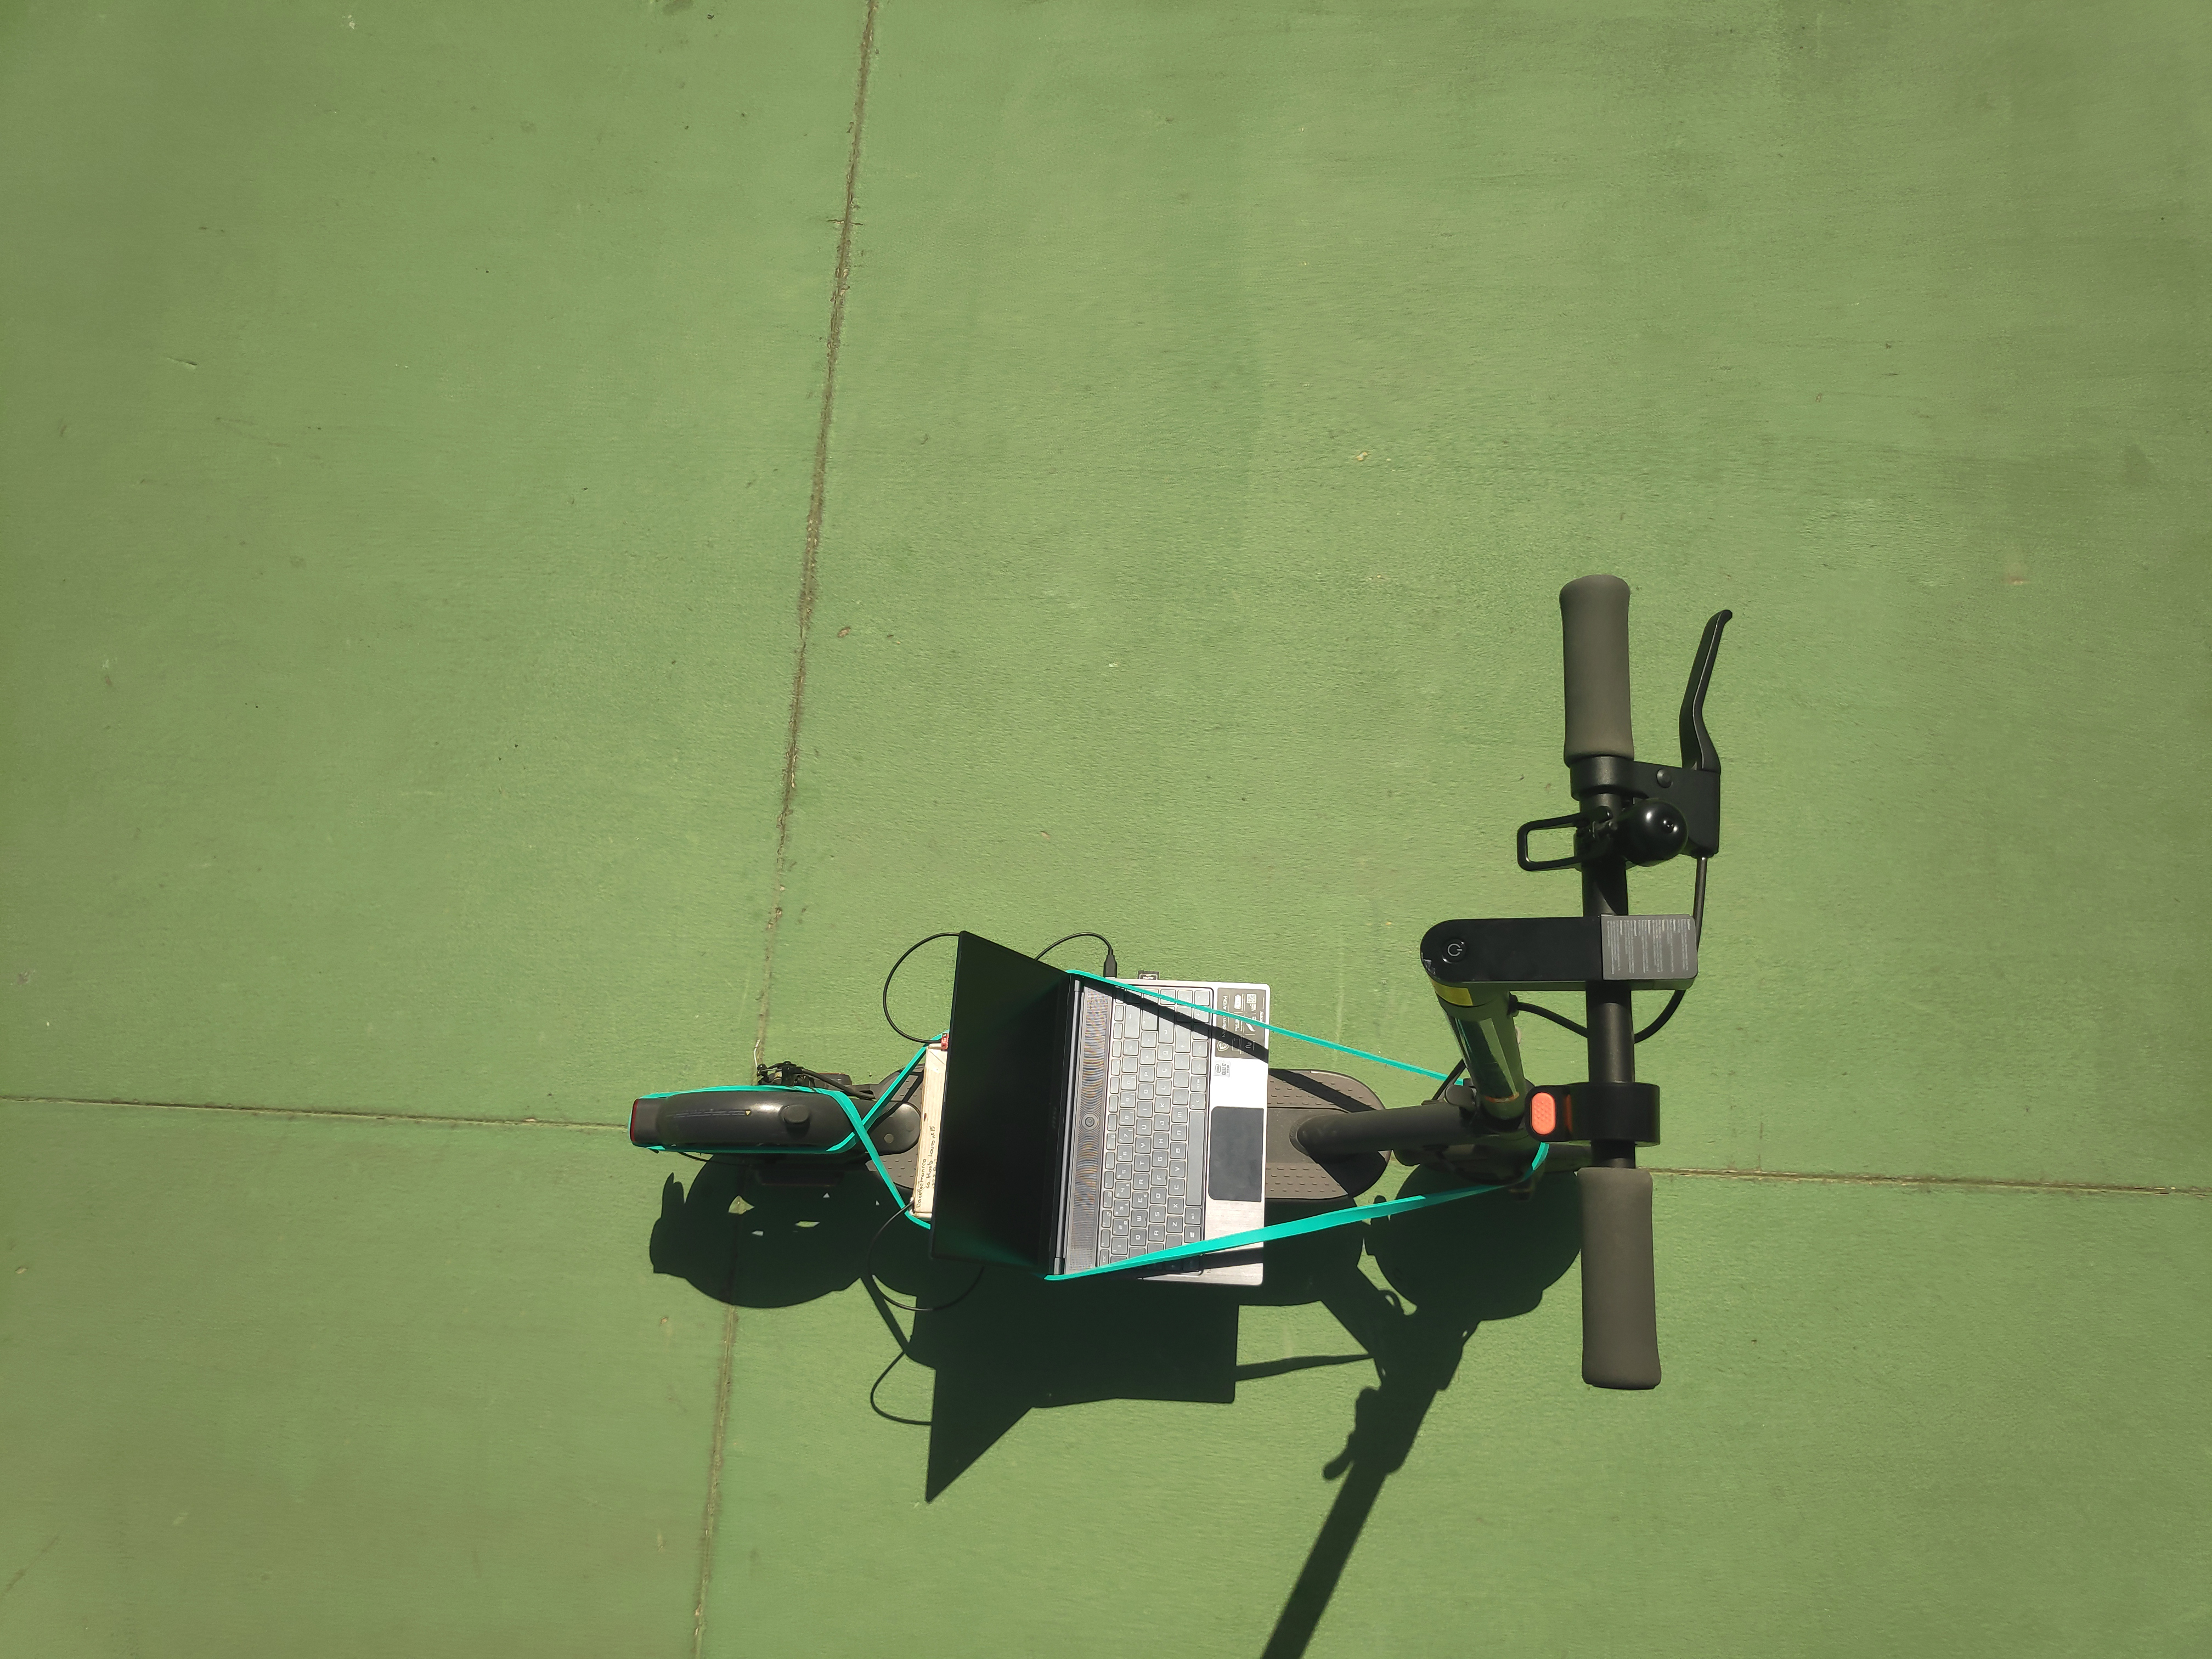
\includegraphics[width=0.9\textwidth]{figures/outdoor.jpg}
    \caption{ 5 meter side ground square used for baseline of accuracy of inertial system. }
    \label{fig:outdoor}
\end{figure}

\begin{figure}[!h]
    \centering
    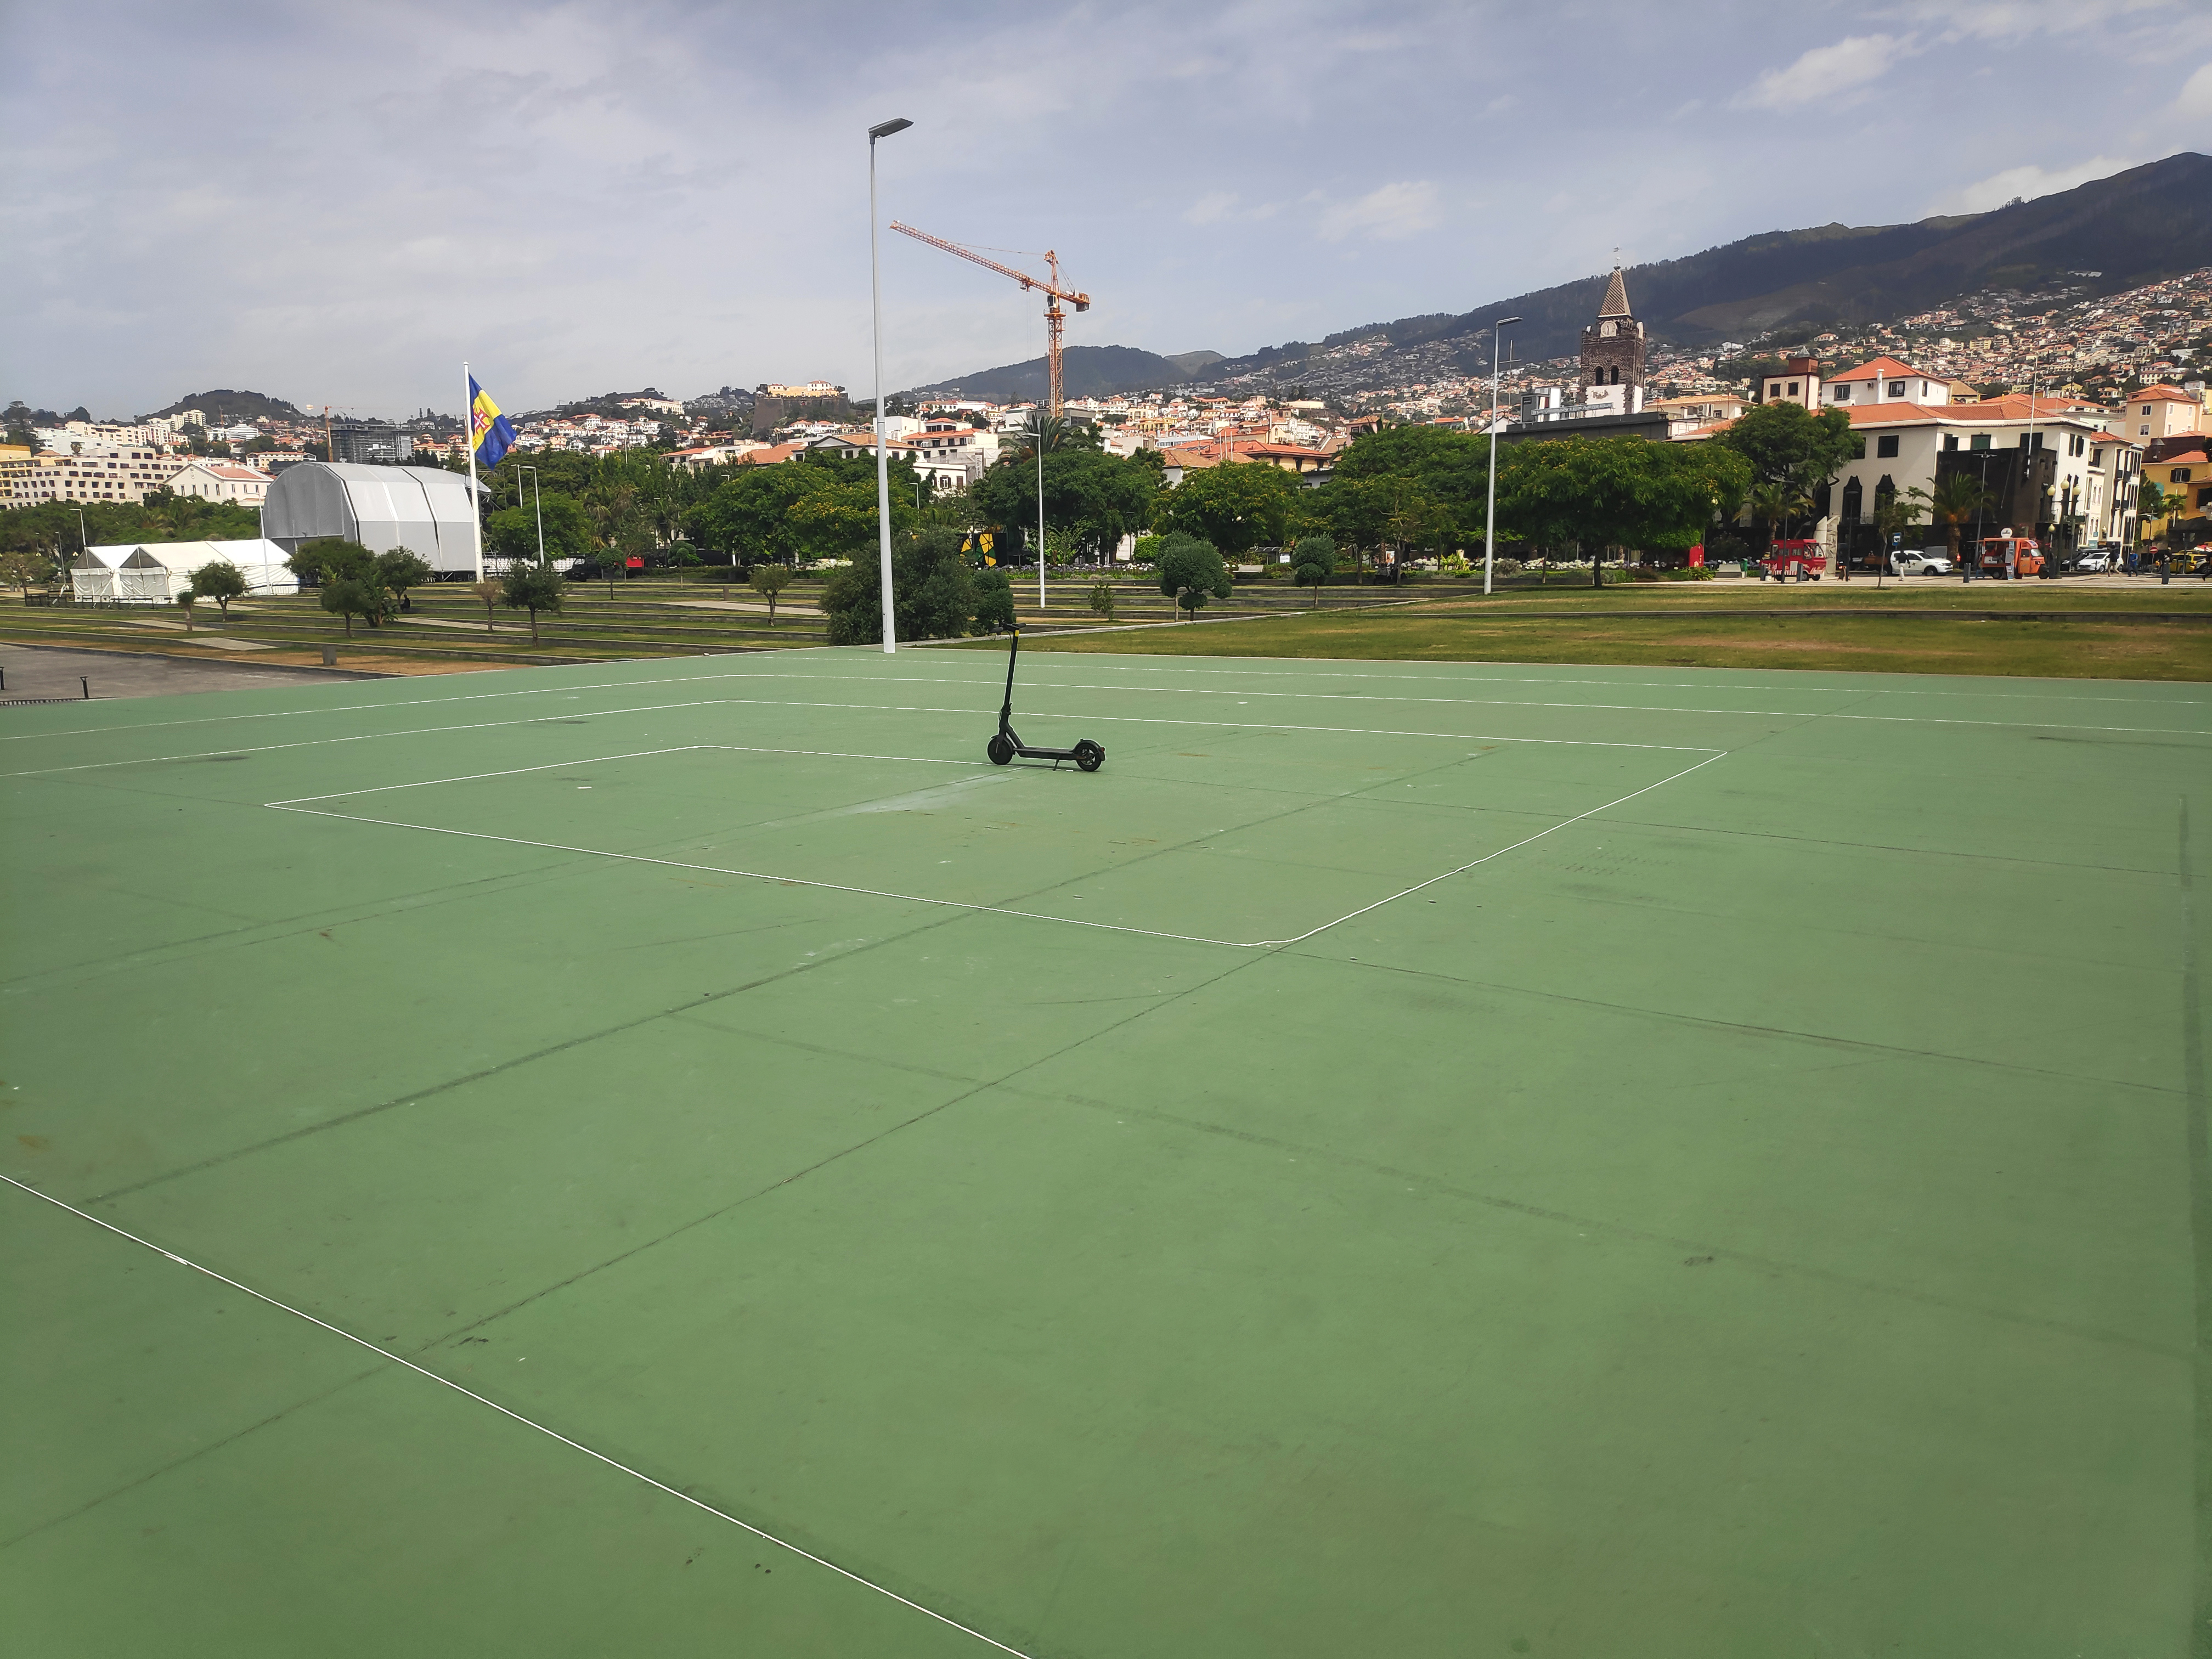
\includegraphics[width=0.9\textwidth]{figures/outdoor_1.jpg}
    \caption{ Manually pulling the skateboard on each side of the ground square. }
    \label{fig:outdoor_1}
\end{figure}

\begin{figure}[!h]
    \centering
    \begin{subfigure}{0.49\textwidth}
        \centering
        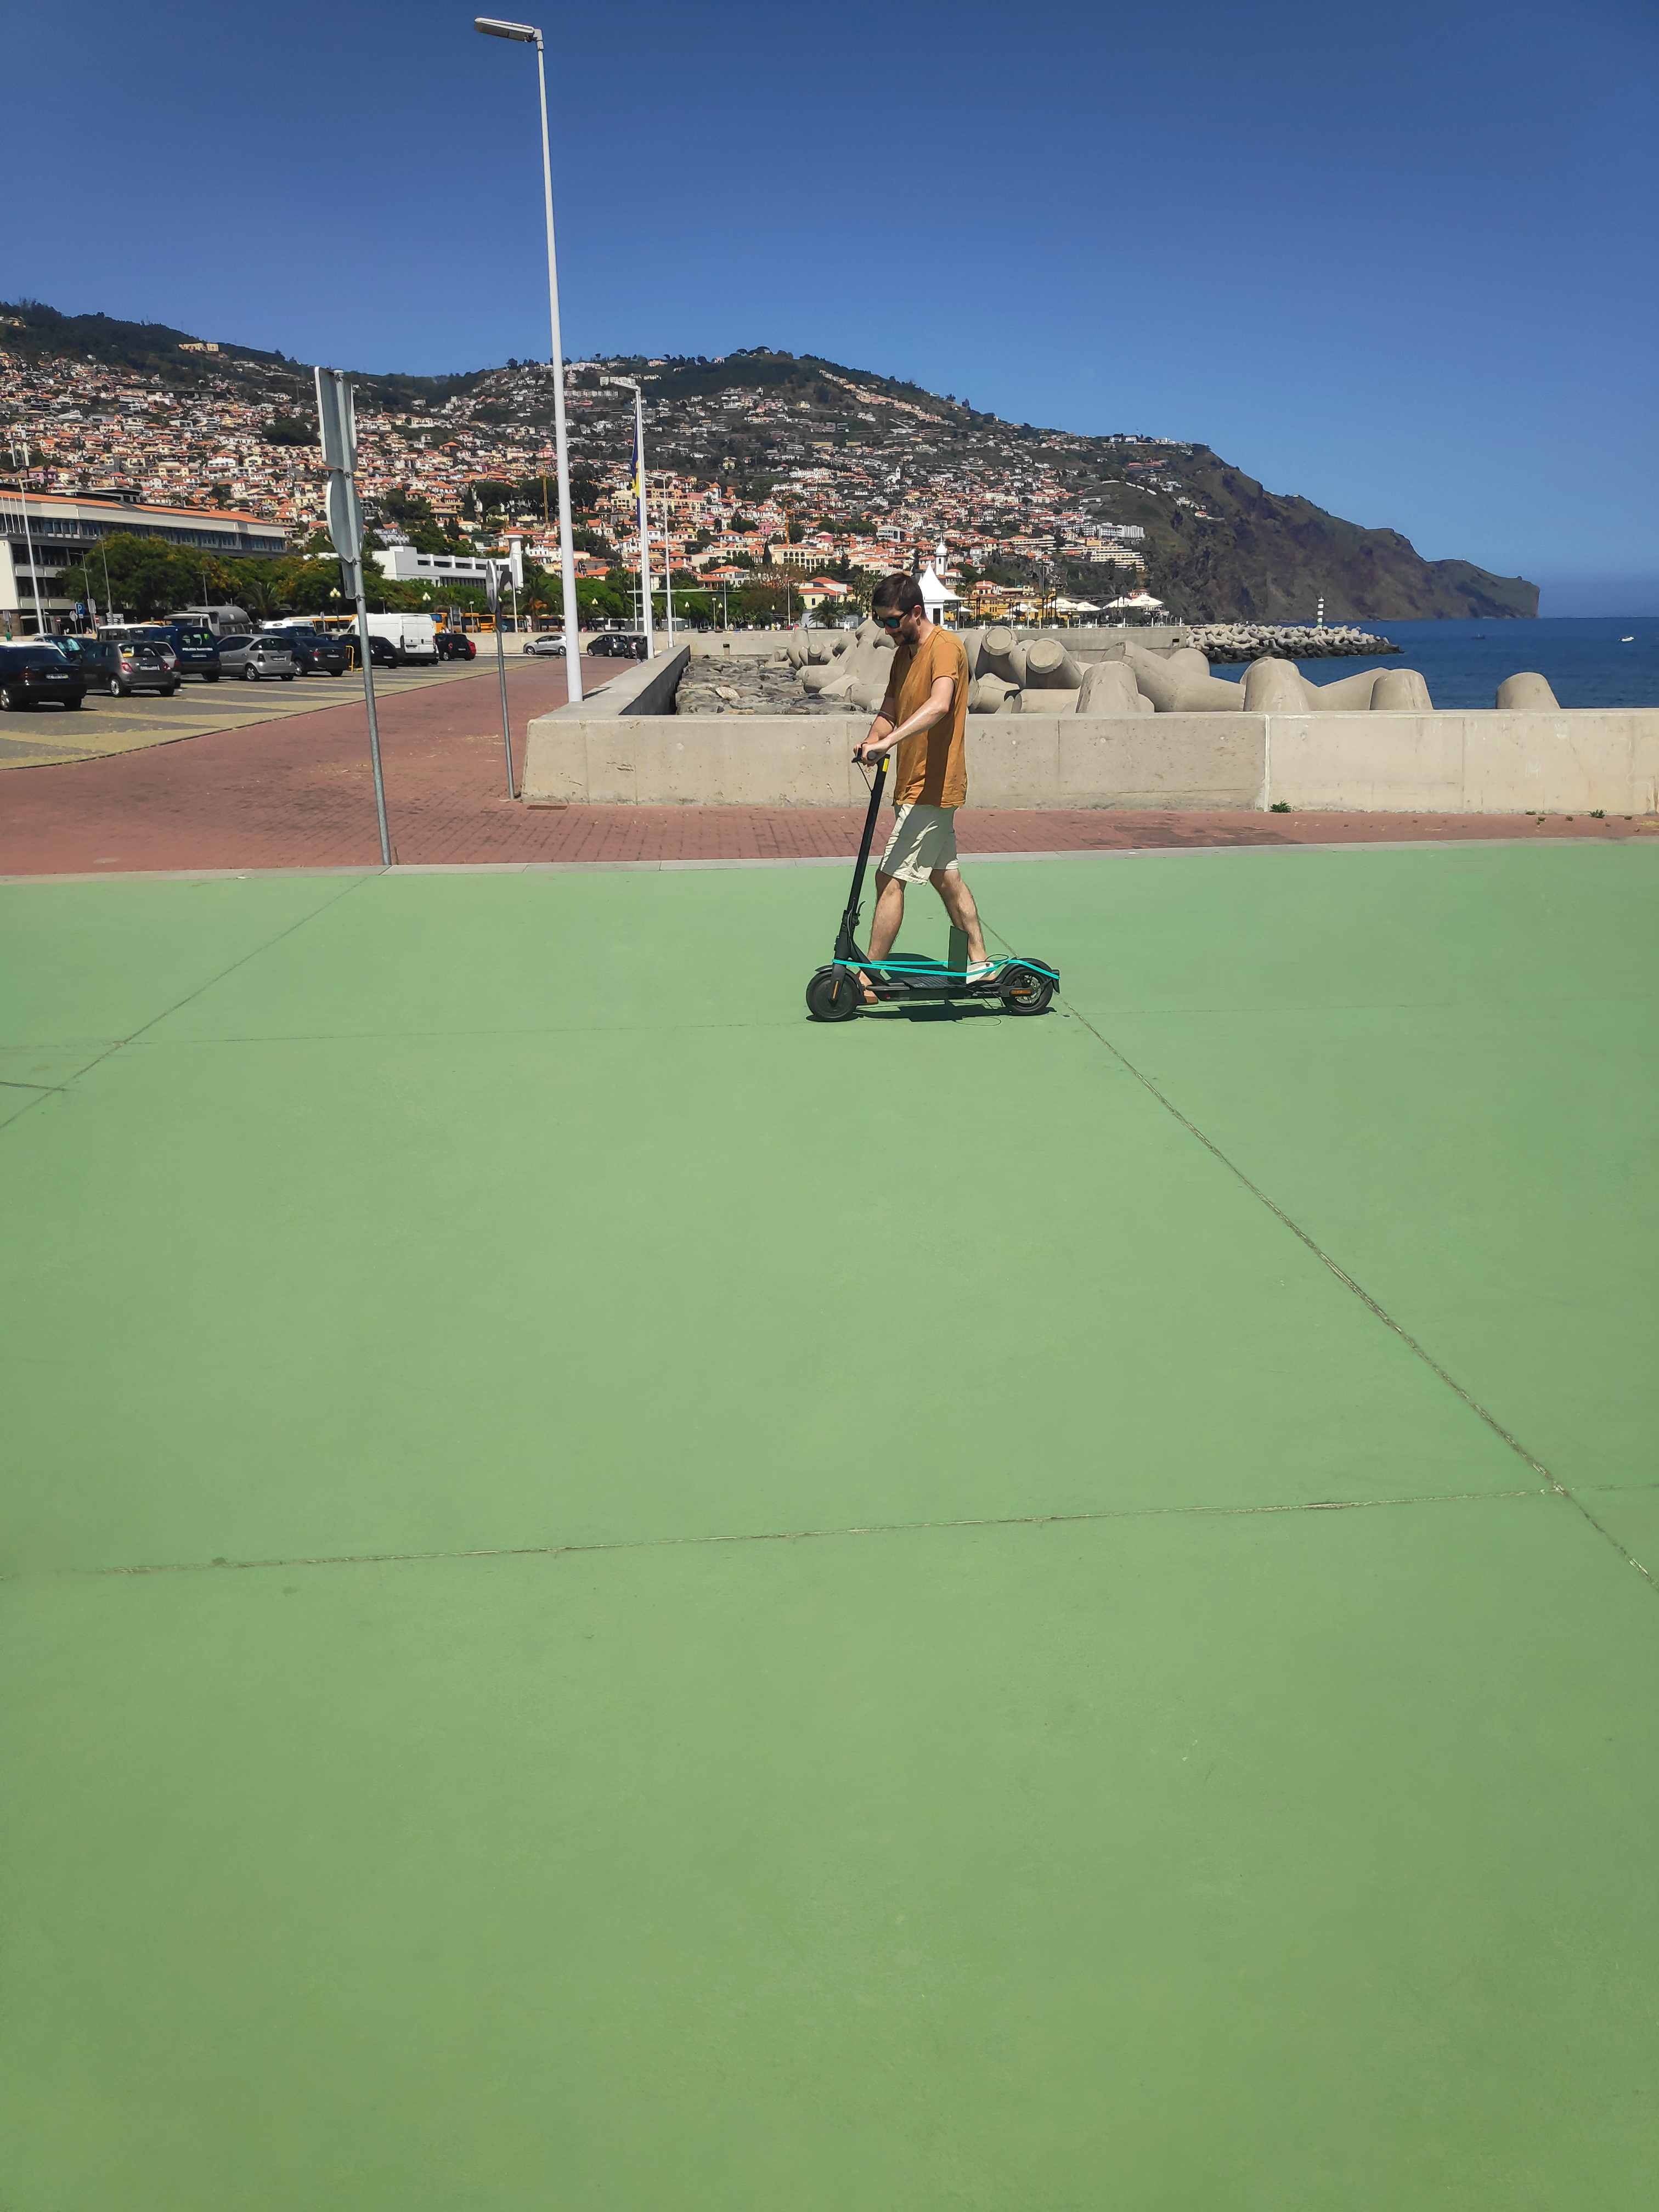
\includegraphics[width=1\textwidth]{figures/outdoor_2.jpg}
        \caption{5 meter side ground square used for baseline of accuracy of inertial system.}
        \label{fig:outdoor_2}
    \end{subfigure}
    \begin{subfigure}{0.49\textwidth}
        \centering
        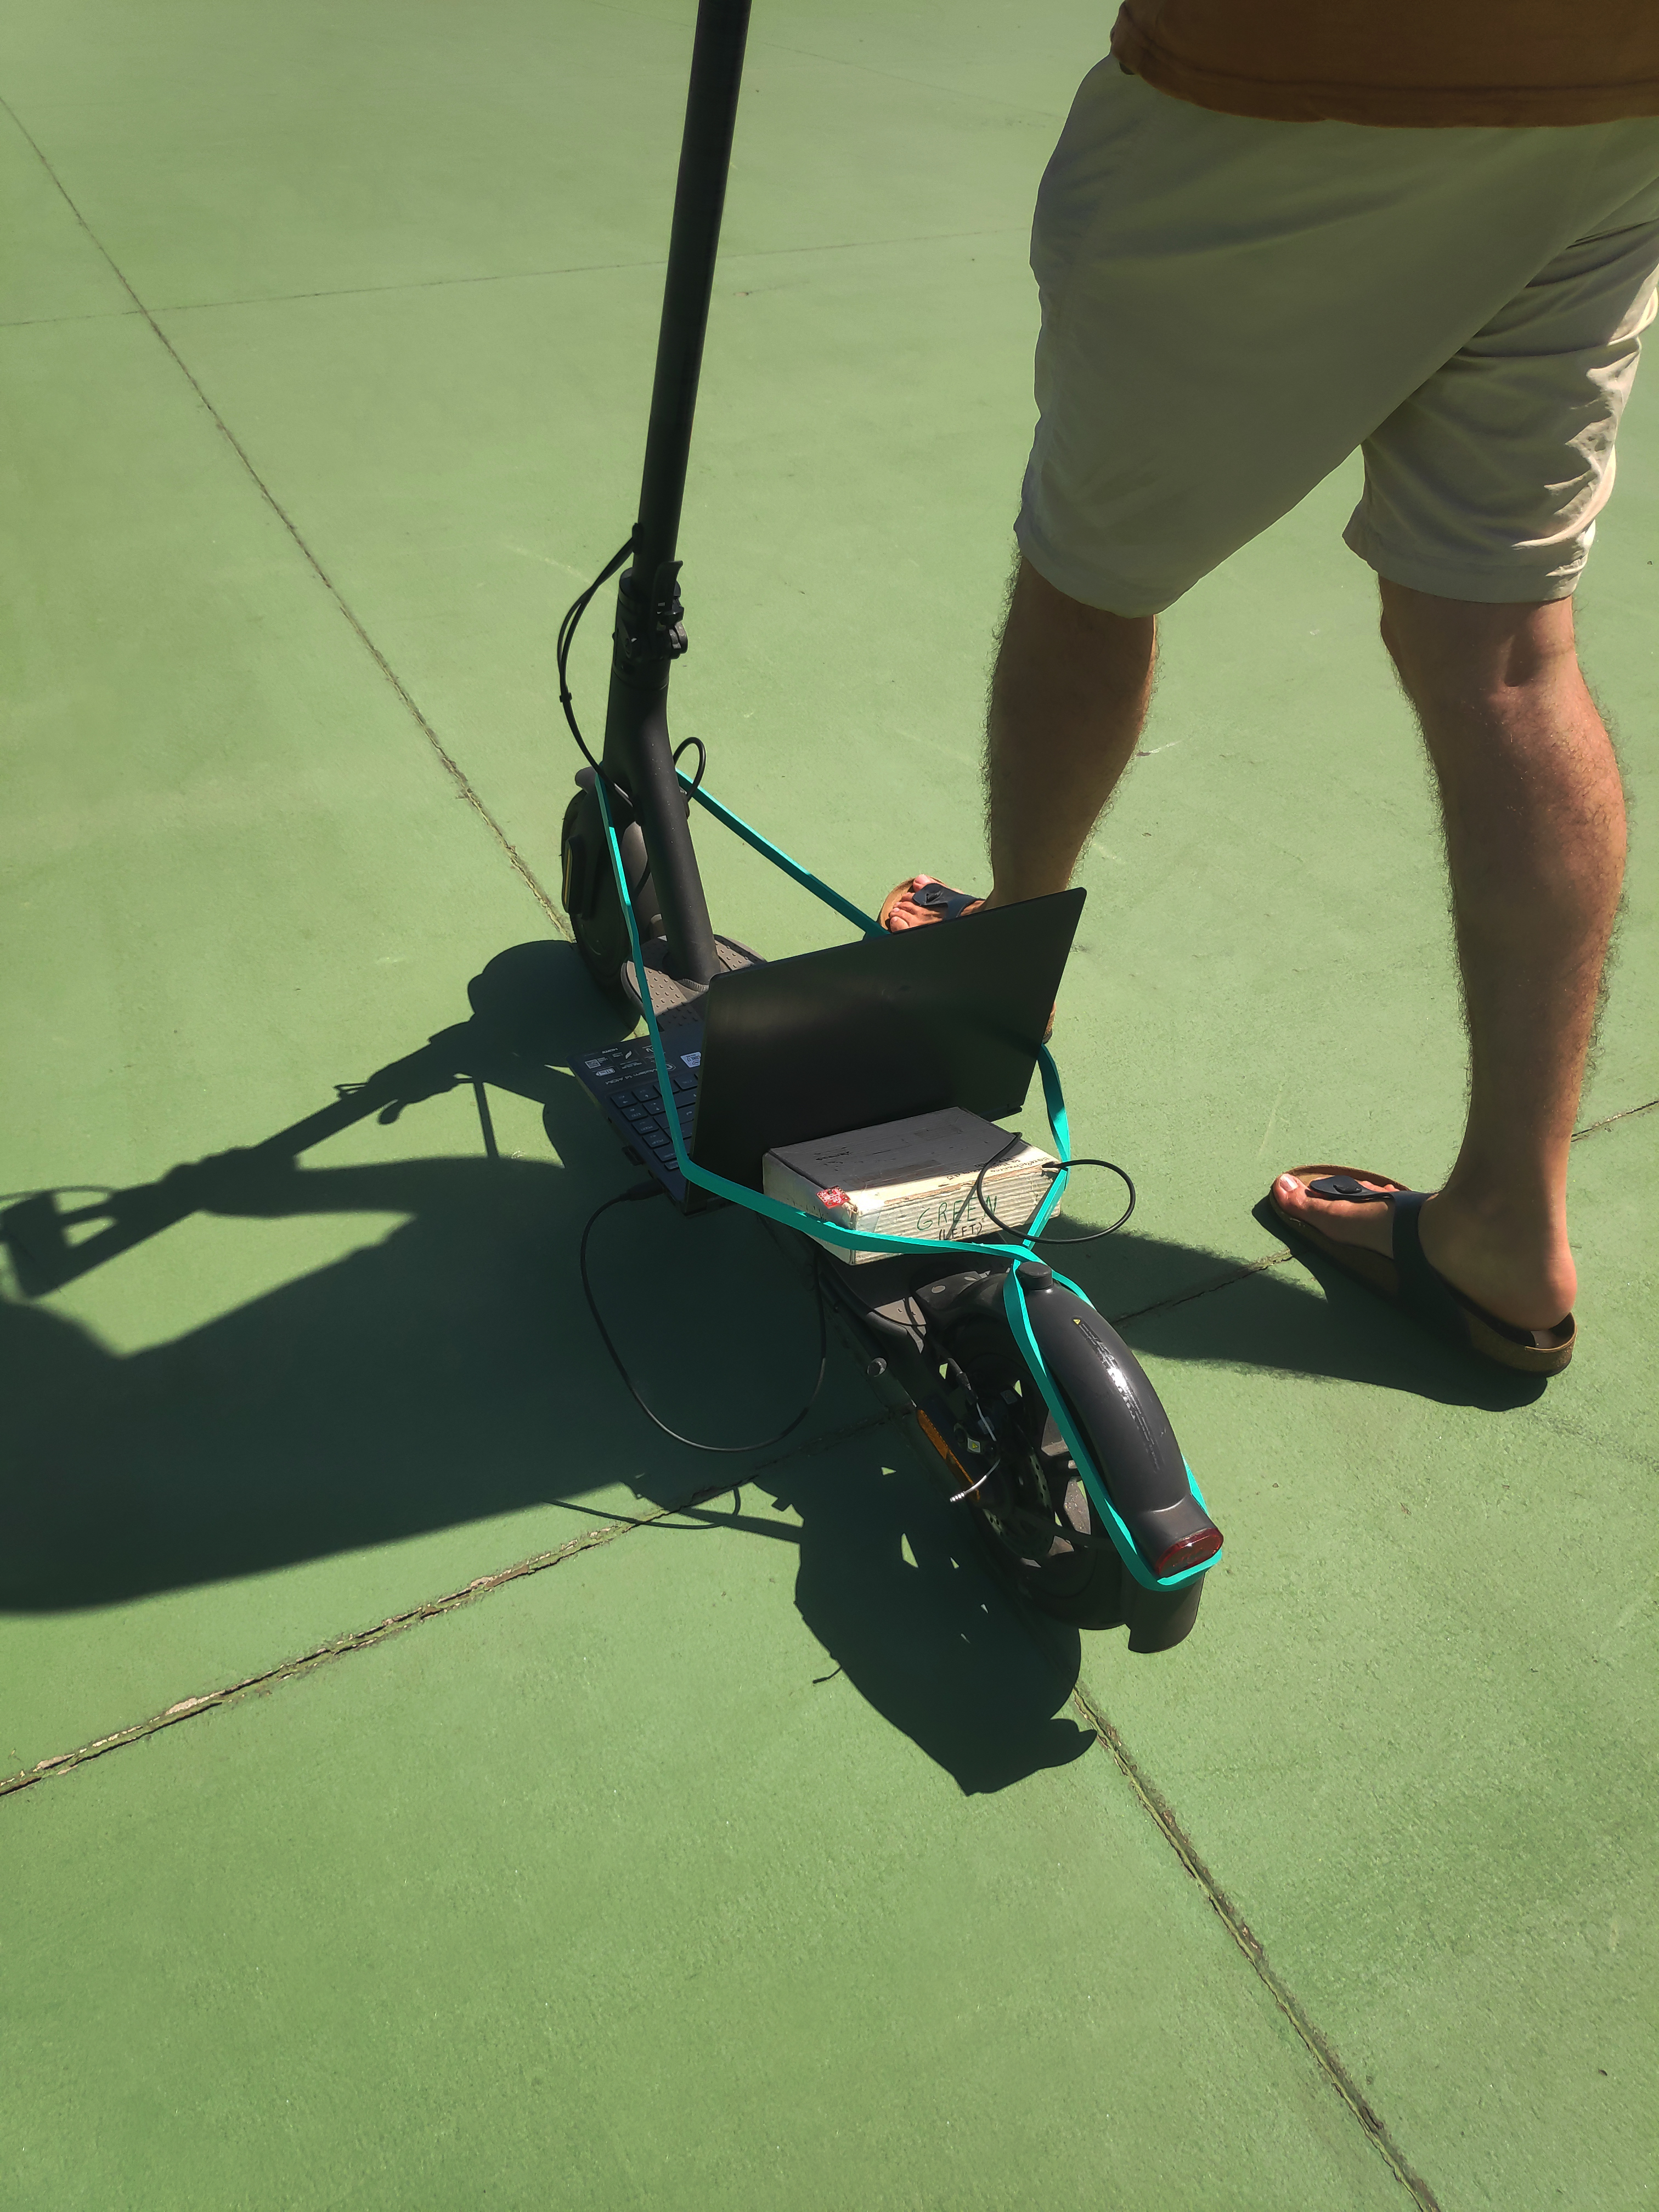
\includegraphics[width=1\textwidth]{figures/outdoor_3.jpg}
        \caption{ Manually pulling the skateboard on each side of the ground square. }
        \label{fig:outdoor_3}
    \end{subfigure}
    \caption{Pin connection between the microcontroller (left) and the IMU (right). Modules are linked through SCL, CLK, VDD and GND pins.}
    \label{fig:hardware}
\end{figure}